%**************************************%
%*    Generated from PreTeXt source   *%
%*    on 2020-05-16T10:09:02-04:00    *%
%*                                    *%
%*      https://pretextbook.org       *%
%*                                    *%
%**************************************%
\documentclass[oneside,10pt,]{book}
%% Custom Preamble Entries, early (use latex.preamble.early)
%% Default LaTeX packages
%%   1.  always employed (or nearly so) for some purpose, or
%%   2.  a stylewriter may assume their presence
\usepackage{geometry}
%% Some aspects of the preamble are conditional,
%% the LaTeX engine is one such determinant
\usepackage{ifthen}
%% etoolbox has a variety of modern conveniences
\usepackage{etoolbox}
\usepackage{ifxetex,ifluatex}
%% Raster graphics inclusion
\usepackage{graphicx}
%% Color support, xcolor package
%% Always loaded, for: add/delete text, author tools
%% Here, since tcolorbox loads tikz, and tikz loads xcolor
\PassOptionsToPackage{usenames,dvipsnames,svgnames,table}{xcolor}
\usepackage{xcolor}
%% begin: defined colors, via xcolor package, for styling
%% end: defined colors, via xcolor package, for styling
%% Colored boxes, and much more, though mostly styling
%% skins library provides "enhanced" skin, employing tikzpicture
%% boxes may be configured as "breakable" or "unbreakable"
%% "raster" controls grids of boxes, aka side-by-side
\usepackage{tcolorbox}
\tcbuselibrary{skins}
\tcbuselibrary{breakable}
\tcbuselibrary{raster}
%% We load some "stock" tcolorbox styles that we use a lot
%% Placement here is provisional, there will be some color work also
%% First, black on white, no border, transparent, but no assumption about titles
\tcbset{ bwminimalstyle/.style={size=minimal, boxrule=-0.3pt, frame empty,
colback=white, colbacktitle=white, coltitle=black, opacityfill=0.0} }
%% Second, bold title, run-in to text/paragraph/heading
%% Space afterwards will be controlled by environment,
%% independent of constructions of the tcb title
%% Places \blocktitlefont onto many block titles
\tcbset{ runintitlestyle/.style={fonttitle=\blocktitlefont\upshape\bfseries, attach title to upper} }
%% Spacing prior to each exercise, anywhere
\tcbset{ exercisespacingstyle/.style={before skip={1.5ex plus 0.5ex}} }
%% Spacing prior to each block
\tcbset{ blockspacingstyle/.style={before skip={2.0ex plus 0.5ex}} }
%% xparse allows the construction of more robust commands,
%% this is a necessity for isolating styling and behavior
%% The tcolorbox library of the same name loads the base library
\tcbuselibrary{xparse}
%% Hyperref should be here, but likes to be loaded late
%%
%% Inline math delimiters, \(, \), need to be robust
%% 2016-01-31:  latexrelease.sty  supersedes  fixltx2e.sty
%% If  latexrelease.sty  exists, bugfix is in kernel
%% If not, bugfix is in  fixltx2e.sty
%% See:  https://tug.org/TUGboat/tb36-3/tb114ltnews22.pdf
%% and read "Fewer fragile commands" in distribution's  latexchanges.pdf
\IfFileExists{latexrelease.sty}{}{\usepackage{fixltx2e}}
%% shorter subnumbers in some side-by-side require manipulations
\usepackage{xstring}
%% Text height identically 9 inches, text width varies on point size
%% See Bringhurst 2.1.1 on measure for recommendations
%% 75 characters per line (count spaces, punctuation) is target
%% which is the upper limit of Bringhurst's recommendations
\geometry{letterpaper,total={340pt,9.0in}}
%% Custom Page Layout Adjustments (use latex.geometry)
%% This LaTeX file may be compiled with pdflatex, xelatex, or lualatex executables
%% LuaTeX is not explicitly supported, but we do accept additions from knowledgeable users
%% The conditional below provides  pdflatex  specific configuration last
%% begin: engine-specific capabilities
\ifthenelse{\boolean{xetex} \or \boolean{luatex}}{%
%% begin: xelatex and lualatex-specific default configuration
\ifxetex\usepackage{xltxtra}\fi
%% realscripts is the only part of xltxtra relevant to lualatex 
\ifluatex\usepackage{realscripts}\fi
%% end:   xelatex and lualatex-specific default configuration
}{
%% begin: pdflatex-specific default configuration
%% We assume a PreTeXt XML source file may have Unicode characters
%% and so we ask LaTeX to parse a UTF-8 encoded file
%% This may work well for accented characters in Western language,
%% but not with Greek, Asian languages, etc.
%% When this is not good enough, switch to the  xelatex  engine
%% where Unicode is better supported (encouraged, even)
\usepackage[utf8]{inputenc}
%% end: pdflatex-specific default configuration
}
%% end:   engine-specific capabilities
%%
%% Fonts.  Conditional on LaTex engine employed.
%% Default Text Font: The Latin Modern fonts are
%% "enhanced versions of the [original TeX] Computer Modern fonts."
%% We use them as the default text font for PreTeXt output.
%% Default Monospace font: Inconsolata (aka zi4)
%% Sponsored by TUG: http://levien.com/type/myfonts/inconsolata.html
%% Loaded for documents with intentional objects requiring monospace
%% See package documentation for excellent instructions
%% fontspec will work universally if we use filename to locate OTF files
%% Loads the "upquote" package as needed, so we don't have to
%% Upright quotes might come from the  textcomp  package, which we also use
%% We employ the shapely \ell to match Google Font version
%% pdflatex: "varl" package option produces shapely \ell
%% pdflatex: "var0" package option produces plain zero (not used)
%% pdflatex: "varqu" package option produces best upright quotes
%% xelatex,lualatex: add OTF StylisticSet 1 for shapely \ell
%% xelatex,lualatex: add OTF StylisticSet 2 for plain zero (not used)
%% xelatex,lualatex: add OTF StylisticSet 3 for upright quotes
%%
%% Automatic Font Control
%% Portions of a document, are, or may, be affected by defined commands
%% These are perhaps more flexible when using  xelatex  rather than  pdflatex
%% The following definitions are meant to be re-defined in a style, using \renewcommand
%% They are scoped when employed (in a TeX group), and so should not be defined with an argument
\newcommand{\divisionfont}{\relax}
\newcommand{\blocktitlefont}{\relax}
\newcommand{\contentsfont}{\relax}
\newcommand{\pagefont}{\relax}
\newcommand{\tabularfont}{\relax}
\newcommand{\xreffont}{\relax}
\newcommand{\titlepagefont}{\relax}
%%
\ifthenelse{\boolean{xetex} \or \boolean{luatex}}{%
%% begin: font setup and configuration for use with xelatex
%% Generally, xelatex is necessary for non-Western fonts
%% fontspec package provides extensive control of system fonts,
%% meaning *.otf (OpenType), and apparently *.ttf (TrueType)
%% that live *outside* your TeX/MF tree, and are controlled by your *system*
%% (it is possible that a TeX distribution will place fonts in a system location)
%%
%% The fontspec package is the best vehicle for using different fonts in  xelatex
%% So we load it always, no matter what a publisher or style might want
%%
\usepackage{fontspec}
%%
%% begin: xelatex main font ("font-xelatex-main" template)
%% Latin Modern Roman is the default font for xelatex and so is loaded with a TU encoding
%% *in the format* so we can't touch it, only perhaps adjust it later
%% in one of two ways (then known by NFSS names such as "lmr")
%% (1) via NFSS with font family names such as "lmr" and "lmss"
%% (2) via fontspec with commands like \setmainfont{Latin Modern Roman}
%% The latter requires the font to be known at the system-level by its font name,
%% but will give access to OTF font features through optional arguments
%% https://tex.stackexchange.com/questions/470008/
%% where-and-how-does-fontspec-sty-specify-the-default-font-latin-modern-roman
%% http://tex.stackexchange.com/questions/115321
%% /how-to-optimize-latin-modern-font-with-xelatex
%%
%% end:   xelatex main font ("font-xelatex-main" template)
%% begin: xelatex mono font ("font-xelatex-mono" template)
%% (conditional on non-trivial uses being present in source)
\IfFontExistsTF{Inconsolatazi4-Regular.otf}{}{\GenericError{}{The font "Inconsolatazi4-Regular.otf" requested by PreTeXt output is not available.  Either a file cannot be located in default locations via a filename, or a font is not known by its name as part of your system.}{Consult the PreTeXt Guide for help with LaTeX fonts.}{}}
\IfFontExistsTF{Inconsolatazi4-Bold.otf}{}{\GenericError{}{The font "Inconsolatazi4-Bold.otf" requested by PreTeXt output is not available.  Either a file cannot be located in default locations via a filename, or a font is not known by its name as part of your system.}{Consult the PreTeXt Guide for help with LaTeX fonts.}{}}
\usepackage{zi4}
\setmonofont[BoldFont=Inconsolatazi4-Bold.otf,StylisticSet={1,3}]{Inconsolatazi4-Regular.otf}
%% end:   xelatex mono font ("font-xelatex-mono" template)
%% begin: xelatex font adjustments ("font-xelatex-style" template)
%% end:   xelatex font adjustments ("font-xelatex-style" template)
%%
%% Extensive support for other languages
\usepackage{polyglossia}
%% Set main/default language based on pretext/@xml:lang value
%% document language code is "en-US", US English
%% usmax variant has extra hypenation
\setmainlanguage[variant=usmax]{english}
%% Enable secondary languages based on discovery of @xml:lang values
%% Enable fonts/scripts based on discovery of @xml:lang values
%% Western languages should be ably covered by Latin Modern Roman
%% end:   font setup and configuration for use with xelatex
}{%
%% begin: font setup and configuration for use with pdflatex
%% begin: pdflatex main font ("font-pdflatex-main" template)
\usepackage{lmodern}
\usepackage[T1]{fontenc}
%% end:   pdflatex main font ("font-pdflatex-main" template)
%% begin: pdflatex mono font ("font-pdflatex-mono" template)
%% (conditional on non-trivial uses being present in source)
\usepackage[varqu,varl]{inconsolata}
%% end:   pdflatex mono font ("font-pdflatex-mono" template)
%% begin: pdflatex font adjustments ("font-pdflatex-style" template)
%% end:   pdflatex font adjustments ("font-pdflatex-style" template)
%% end:   font setup and configuration for use with pdflatex
}
%% Symbols, align environment, commutative diagrams, bracket-matrix
\usepackage{amsmath}
\usepackage{amscd}
\usepackage{amssymb}
%% allow page breaks within display mathematics anywhere
%% level 4 is maximally permissive
%% this is exactly the opposite of AMSmath package philosophy
%% there are per-display, and per-equation options to control this
%% split, aligned, gathered, and alignedat are not affected
\allowdisplaybreaks[4]
%% allow more columns to a matrix
%% can make this even bigger by overriding with  latex.preamble.late  processing option
\setcounter{MaxMatrixCols}{30}
%%
%%
%% Division Titles, and Page Headers/Footers
%% titlesec package, loading "titleps" package cooperatively
%% See code comments about the necessity and purpose of "explicit" option.
%% The "newparttoc" option causes a consistent entry for parts in the ToC 
%% file, but it is only effective if there is a \titleformat for \part.
%% "pagestyles" loads the  titleps  package cooperatively.
\usepackage[explicit, newparttoc, pagestyles]{titlesec}
%% The companion titletoc package for the ToC.
\usepackage{titletoc}
%% Fixes a bug with transition from chapters to appendices in a "book"
%% See generating XSL code for more details about necessity
\newtitlemark{\chaptertitlename}
%% begin: customizations of page styles via the modal "titleps-style" template
%% Designed to use commands from the LaTeX "titleps" package
%% Plain pages should have the same font for page numbers
\renewpagestyle{plain}{%
\setfoot{}{\pagefont\thepage}{}%
}%
%% Single pages as in default LaTeX
\renewpagestyle{headings}{%
\sethead{\pagefont\slshape\MakeUppercase{\ifthechapter{\chaptertitlename\space\thechapter.\space}{}\chaptertitle}}{}{\pagefont\thepage}%
}%
\pagestyle{headings}
%% end: customizations of page styles via the modal "titleps-style" template
%%
%% Create globally-available macros to be provided for style writers
%% These are redefined for each occurence of each division
\newcommand{\divisionnameptx}{\relax}%
\newcommand{\titleptx}{\relax}%
\newcommand{\subtitleptx}{\relax}%
\newcommand{\shortitleptx}{\relax}%
\newcommand{\authorsptx}{\relax}%
\newcommand{\epigraphptx}{\relax}%
%% Create environments for possible occurences of each division
%% Environment for a PTX "acknowledgement" at the level of a LaTeX "chapter"
\NewDocumentEnvironment{acknowledgement}{mmmmmm}
{%
\renewcommand{\divisionnameptx}{Acknowledgements}%
\renewcommand{\titleptx}{#1}%
\renewcommand{\subtitleptx}{#2}%
\renewcommand{\shortitleptx}{#3}%
\renewcommand{\authorsptx}{#4}%
\renewcommand{\epigraphptx}{#5}%
\chapter*{#1}%
\addcontentsline{toc}{chapter}{#3}
\label{#6}%
}{}%
%% Environment for a PTX "preface" at the level of a LaTeX "chapter"
\NewDocumentEnvironment{preface}{mmmmmm}
{%
\renewcommand{\divisionnameptx}{Preface}%
\renewcommand{\titleptx}{#1}%
\renewcommand{\subtitleptx}{#2}%
\renewcommand{\shortitleptx}{#3}%
\renewcommand{\authorsptx}{#4}%
\renewcommand{\epigraphptx}{#5}%
\chapter*{#1}%
\addcontentsline{toc}{chapter}{#3}
\label{#6}%
}{}%
%% Environment for a PTX "chapter" at the level of a LaTeX "chapter"
\NewDocumentEnvironment{chapterptx}{mmmmmm}
{%
\renewcommand{\divisionnameptx}{Chapter}%
\renewcommand{\titleptx}{#1}%
\renewcommand{\subtitleptx}{#2}%
\renewcommand{\shortitleptx}{#3}%
\renewcommand{\authorsptx}{#4}%
\renewcommand{\epigraphptx}{#5}%
\chapter[{#3}]{#1}%
\label{#6}%
}{}%
%% Environment for a PTX "section" at the level of a LaTeX "section"
\NewDocumentEnvironment{sectionptx}{mmmmmm}
{%
\renewcommand{\divisionnameptx}{Section}%
\renewcommand{\titleptx}{#1}%
\renewcommand{\subtitleptx}{#2}%
\renewcommand{\shortitleptx}{#3}%
\renewcommand{\authorsptx}{#4}%
\renewcommand{\epigraphptx}{#5}%
\section[{#3}]{#1}%
\label{#6}%
}{}%
%% Environment for a PTX "subsection" at the level of a LaTeX "subsection"
\NewDocumentEnvironment{subsectionptx}{mmmmmm}
{%
\renewcommand{\divisionnameptx}{Subsection}%
\renewcommand{\titleptx}{#1}%
\renewcommand{\subtitleptx}{#2}%
\renewcommand{\shortitleptx}{#3}%
\renewcommand{\authorsptx}{#4}%
\renewcommand{\epigraphptx}{#5}%
\subsection[{#3}]{#1}%
\label{#6}%
}{}%
%% Environment for a PTX "exercises" at the level of a LaTeX "subsection"
\NewDocumentEnvironment{exercises-subsection}{mmmmmm}
{%
\renewcommand{\divisionnameptx}{Exercises}%
\renewcommand{\titleptx}{#1}%
\renewcommand{\subtitleptx}{#2}%
\renewcommand{\shortitleptx}{#3}%
\renewcommand{\authorsptx}{#4}%
\renewcommand{\epigraphptx}{#5}%
\subsection[{#3}]{#1}%
\label{#6}%
}{}%
%% Environment for a PTX "exercises" at the level of a LaTeX "subsection"
\NewDocumentEnvironment{exercises-subsection-numberless}{mmmmmm}
{%
\renewcommand{\divisionnameptx}{Exercises}%
\renewcommand{\titleptx}{#1}%
\renewcommand{\subtitleptx}{#2}%
\renewcommand{\shortitleptx}{#3}%
\renewcommand{\authorsptx}{#4}%
\renewcommand{\epigraphptx}{#5}%
\subsection*{#1}%
\addcontentsline{toc}{subsection}{#3}
\label{#6}%
}{}%
%% Environment for a PTX "subsubsection" at the level of a LaTeX "subsubsection"
\NewDocumentEnvironment{subsubsectionptx}{mmmmmm}
{%
\renewcommand{\divisionnameptx}{Subsubsection}%
\renewcommand{\titleptx}{#1}%
\renewcommand{\subtitleptx}{#2}%
\renewcommand{\shortitleptx}{#3}%
\renewcommand{\authorsptx}{#4}%
\renewcommand{\epigraphptx}{#5}%
\subsubsection[{#3}]{#1}%
\label{#6}%
}{}%
%% Environment for a PTX "references" at the level of a LaTeX "subsection"
\NewDocumentEnvironment{references-subsection}{mmmmmm}
{%
\renewcommand{\divisionnameptx}{References}%
\renewcommand{\titleptx}{#1}%
\renewcommand{\subtitleptx}{#2}%
\renewcommand{\shortitleptx}{#3}%
\renewcommand{\authorsptx}{#4}%
\renewcommand{\epigraphptx}{#5}%
\subsection[{#3}]{#1}%
\label{#6}%
}{}%
%% Environment for a PTX "references" at the level of a LaTeX "subsection"
\NewDocumentEnvironment{references-subsection-numberless}{mmmmmm}
{%
\renewcommand{\divisionnameptx}{References}%
\renewcommand{\titleptx}{#1}%
\renewcommand{\subtitleptx}{#2}%
\renewcommand{\shortitleptx}{#3}%
\renewcommand{\authorsptx}{#4}%
\renewcommand{\epigraphptx}{#5}%
\subsection*{#1}%
\addcontentsline{toc}{subsection}{#3}
\label{#6}%
}{}%
%% Environment for a PTX "appendix" at the level of a LaTeX "chapter"
\NewDocumentEnvironment{appendixptx}{mmmmmm}
{%
\renewcommand{\divisionnameptx}{Appendix}%
\renewcommand{\titleptx}{#1}%
\renewcommand{\subtitleptx}{#2}%
\renewcommand{\shortitleptx}{#3}%
\renewcommand{\authorsptx}{#4}%
\renewcommand{\epigraphptx}{#5}%
\chapter[{#3}]{#1}%
\label{#6}%
}{}%
%% Environment for a PTX "solutions" at the level of a LaTeX "chapter"
\NewDocumentEnvironment{solutions-chapter}{mmmmmm}
{%
\renewcommand{\divisionnameptx}{Appendix}%
\renewcommand{\titleptx}{#1}%
\renewcommand{\subtitleptx}{#2}%
\renewcommand{\shortitleptx}{#3}%
\renewcommand{\authorsptx}{#4}%
\renewcommand{\epigraphptx}{#5}%
\chapter[{#3}]{#1}%
\label{#6}%
}{}%
%% Environment for a PTX "solutions" at the level of a LaTeX "chapter"
\NewDocumentEnvironment{solutions-chapter-numberless}{mmmmmm}
{%
\renewcommand{\divisionnameptx}{Appendix}%
\renewcommand{\titleptx}{#1}%
\renewcommand{\subtitleptx}{#2}%
\renewcommand{\shortitleptx}{#3}%
\renewcommand{\authorsptx}{#4}%
\renewcommand{\epigraphptx}{#5}%
\chapter*{#1}%
\addcontentsline{toc}{chapter}{#3}
\label{#6}%
}{}%
%% Environment for a PTX "references" at the level of a LaTeX "chapter"
\NewDocumentEnvironment{references-chapter}{mmmmmm}
{%
\renewcommand{\divisionnameptx}{References}%
\renewcommand{\titleptx}{#1}%
\renewcommand{\subtitleptx}{#2}%
\renewcommand{\shortitleptx}{#3}%
\renewcommand{\authorsptx}{#4}%
\renewcommand{\epigraphptx}{#5}%
\chapter[{#3}]{#1}%
\label{#6}%
}{}%
%% Environment for a PTX "references" at the level of a LaTeX "chapter"
\NewDocumentEnvironment{references-chapter-numberless}{mmmmmm}
{%
\renewcommand{\divisionnameptx}{References}%
\renewcommand{\titleptx}{#1}%
\renewcommand{\subtitleptx}{#2}%
\renewcommand{\shortitleptx}{#3}%
\renewcommand{\authorsptx}{#4}%
\renewcommand{\epigraphptx}{#5}%
\chapter*{#1}%
\addcontentsline{toc}{chapter}{#3}
\label{#6}%
}{}%
%% Environment for a PTX "index" at the level of a LaTeX "chapter"
\NewDocumentEnvironment{indexptx}{mmmmmm}
{%
\renewcommand{\divisionnameptx}{Index}%
\renewcommand{\titleptx}{#1}%
\renewcommand{\subtitleptx}{#2}%
\renewcommand{\shortitleptx}{#3}%
\renewcommand{\authorsptx}{#4}%
\renewcommand{\epigraphptx}{#5}%
\chapter*{#1}%
\addcontentsline{toc}{chapter}{#3}
\label{#6}%
}{}%
%%
%% Styles for six traditional LaTeX divisions
\titleformat{\part}[display]
{\divisionfont\Huge\bfseries\centering}{\divisionnameptx\space\thepart}{30pt}{\Huge#1}
[{\Large\centering\authorsptx}]
\titleformat{\chapter}[display]
{\divisionfont\huge\bfseries}{\divisionnameptx\space\thechapter}{20pt}{\Huge#1}
[{\Large\authorsptx}]
\titleformat{name=\chapter,numberless}[display]
{\divisionfont\huge\bfseries}{}{0pt}{#1}
[{\Large\authorsptx}]
\titlespacing*{\chapter}{0pt}{50pt}{40pt}
\titleformat{\section}[hang]
{\divisionfont\Large\bfseries}{\thesection}{1ex}{#1}
[{\large\authorsptx}]
\titleformat{name=\section,numberless}[block]
{\divisionfont\Large\bfseries}{}{0pt}{#1}
[{\large\authorsptx}]
\titlespacing*{\section}{0pt}{3.5ex plus 1ex minus .2ex}{2.3ex plus .2ex}
\titleformat{\subsection}[hang]
{\divisionfont\large\bfseries}{\thesubsection}{1ex}{#1}
[{\normalsize\authorsptx}]
\titleformat{name=\subsection,numberless}[block]
{\divisionfont\large\bfseries}{}{0pt}{#1}
[{\normalsize\authorsptx}]
\titlespacing*{\subsection}{0pt}{3.25ex plus 1ex minus .2ex}{1.5ex plus .2ex}
\titleformat{\subsubsection}[hang]
{\divisionfont\normalsize\bfseries}{\thesubsubsection}{1em}{#1}
[{\small\authorsptx}]
\titleformat{name=\subsubsection,numberless}[block]
{\divisionfont\normalsize\bfseries}{}{0pt}{#1}
[{\normalsize\authorsptx}]
\titlespacing*{\subsubsection}{0pt}{3.25ex plus 1ex minus .2ex}{1.5ex plus .2ex}
\titleformat{\paragraph}[hang]
{\divisionfont\normalsize\bfseries}{\theparagraph}{1em}{#1}
[{\small\authorsptx}]
\titleformat{name=\paragraph,numberless}[block]
{\divisionfont\normalsize\bfseries}{}{0pt}{#1}
[{\normalsize\authorsptx}]
\titlespacing*{\paragraph}{0pt}{3.25ex plus 1ex minus .2ex}{1.5em}
%%
%% Styles for five traditional LaTeX divisions
\titlecontents{part}%
[0pt]{\contentsmargin{0em}\addvspace{1pc}\contentsfont\bfseries}%
{\Large\thecontentslabel\enspace}{\Large}%
{}%
[\addvspace{.5pc}]%
\titlecontents{chapter}%
[0pt]{\contentsmargin{0em}\addvspace{1pc}\contentsfont\bfseries}%
{\large\thecontentslabel\enspace}{\large}%
{\hfill\bfseries\thecontentspage}%
[\addvspace{.5pc}]%
\dottedcontents{section}[3.8em]{\contentsfont}{2.3em}{1pc}%
\dottedcontents{subsection}[6.1em]{\contentsfont}{3.2em}{1pc}%
\dottedcontents{subsubsection}[9.3em]{\contentsfont}{4.3em}{1pc}%
%%
%% Begin: Semantic Macros
%% To preserve meaning in a LaTeX file
%%
%% \mono macro for content of "c", "cd", "tag", etc elements
%% Also used automatically in other constructions
%% Simply an alias for \texttt
%% Always defined, even if there is no need, or if a specific tt font is not loaded
\newcommand{\mono}[1]{\texttt{#1}}
%%
%% Following semantic macros are only defined here if their
%% use is required only in this specific document
%%
%% Used for inline definitions of terms
\newcommand{\terminology}[1]{\textbf{#1}}
%% Arrows for iff proofs, with trailing space
\newcommand{\forwardimplication}{($\Rightarrow$)}
\newcommand{\backwardimplication}{($\Leftarrow$)}
%% End: Semantic Macros
%% Division Numbering: Chapters, Sections, Subsections, etc
%% Division numbers may be turned off at some level ("depth")
%% A section *always* has depth 1, contrary to us counting from the document root
%% The latex default is 3.  If a larger number is present here, then
%% removing this command may make some cross-references ambiguous
%% The precursor variable $numbering-maxlevel is checked for consistency in the common XSL file
\setcounter{secnumdepth}{3}
%%
%% AMS "proof" environment is no longer used, but we leave previously
%% implemented \qedhere in place, should the LaTeX be recycled
\newcommand{\qedhere}{\relax}
%%
%% A faux tcolorbox whose only purpose is to provide common numbering
%% facilities for most blocks (possibly not projects, 2D displays)
%% Controlled by  numbering.theorems.level  processing parameter
\newtcolorbox[auto counter, number within=section]{block}{}
%%
%% This document is set to number PROJECT-LIKE on a separate numbering scheme
%% So, a faux tcolorbox whose only purpose is to provide this numbering
%% Controlled by  numbering.projects.level  processing parameter
\newtcolorbox[auto counter, number within=section]{project-distinct}{}
%% A faux tcolorbox whose only purpose is to provide common numbering
%% facilities for 2D displays which are subnumbered as part of a "sidebyside"
\newtcolorbox[auto counter, number within=tcb@cnt@block, number freestyle={\noexpand\thetcb@cnt@block(\noexpand\alph{\tcbcounter})}]{subdisplay}{}
%%
%% tcolorbox, with styles, for THEOREM-LIKE
%%
%% algorithm: fairly simple numbered block/structure
\tcbset{ algorithmstyle/.style={bwminimalstyle, runintitlestyle, blockspacingstyle, after title={\space}, } }
\newtcolorbox[use counter from=block]{algorithm}[3]{title={{Algorithm~\thetcbcounter\notblank{#1#2}{\space}{}\notblank{#1}{\space#1}{}\notblank{#2}{\space(#2)}{}}}, phantomlabel={#3}, breakable, parbox=false, after={\par}, fontupper=\itshape, algorithmstyle, }
%% theorem: fairly simple numbered block/structure
\tcbset{ theoremstyle/.style={bwminimalstyle, runintitlestyle, blockspacingstyle, after title={\space}, } }
\newtcolorbox[use counter from=block]{theorem}[3]{title={{Theorem~\thetcbcounter\notblank{#1#2}{\space}{}\notblank{#1}{\space#1}{}\notblank{#2}{\space(#2)}{}}}, phantomlabel={#3}, breakable, parbox=false, after={\par}, fontupper=\itshape, theoremstyle, }
%% corollary: fairly simple numbered block/structure
\tcbset{ corollarystyle/.style={bwminimalstyle, runintitlestyle, blockspacingstyle, after title={\space}, } }
\newtcolorbox[use counter from=block]{corollary}[3]{title={{Corollary~\thetcbcounter\notblank{#1#2}{\space}{}\notblank{#1}{\space#1}{}\notblank{#2}{\space(#2)}{}}}, phantomlabel={#3}, breakable, parbox=false, after={\par}, fontupper=\itshape, corollarystyle, }
%% lemma: fairly simple numbered block/structure
\tcbset{ lemmastyle/.style={bwminimalstyle, runintitlestyle, blockspacingstyle, after title={\space}, } }
\newtcolorbox[use counter from=block]{lemma}[3]{title={{Lemma~\thetcbcounter\notblank{#1#2}{\space}{}\notblank{#1}{\space#1}{}\notblank{#2}{\space(#2)}{}}}, phantomlabel={#3}, breakable, parbox=false, after={\par}, fontupper=\itshape, lemmastyle, }
%%
%% tcolorbox, with styles, for AXIOM-LIKE
%%
%% axiom: fairly simple numbered block/structure
\tcbset{ axiomstyle/.style={bwminimalstyle, runintitlestyle, blockspacingstyle, after title={\space}, } }
\newtcolorbox[use counter from=block]{axiom}[3]{title={{Axiom~\thetcbcounter\notblank{#1#2}{\space}{}\notblank{#1}{\space#1}{}\notblank{#2}{\space(#2)}{}}}, phantomlabel={#3}, breakable, parbox=false, after={\par}, fontupper=\itshape, axiomstyle, }
%% heuristic: fairly simple numbered block/structure
\tcbset{ heuristicstyle/.style={bwminimalstyle, runintitlestyle, blockspacingstyle, after title={\space}, } }
\newtcolorbox[use counter from=block]{heuristic}[3]{title={{Heuristic~\thetcbcounter\notblank{#1#2}{\space}{}\notblank{#1}{\space#1}{}\notblank{#2}{\space(#2)}{}}}, phantomlabel={#3}, breakable, parbox=false, after={\par}, fontupper=\itshape, heuristicstyle, }
%%
%% tcolorbox, with styles, for DEFINITION-LIKE
%%
%% definition: fairly simple numbered block/structure
\tcbset{ definitionstyle/.style={bwminimalstyle, runintitlestyle, blockspacingstyle, after title={\space}, after upper={\space\space\hspace*{\stretch{1}}\(\lozenge\)}, } }
\newtcolorbox[use counter from=block]{definition}[2]{title={{Definition~\thetcbcounter\notblank{#1}{\space\space#1}{}}}, phantomlabel={#2}, breakable, parbox=false, after={\par}, definitionstyle, }
%%
%% tcolorbox, with styles, for REMARK-LIKE
%%
%% note: fairly simple numbered block/structure
\tcbset{ notestyle/.style={bwminimalstyle, runintitlestyle, blockspacingstyle, after title={\space}, } }
\newtcolorbox[use counter from=block]{note}[2]{title={{Note~\thetcbcounter\notblank{#1}{\space\space#1}{}}}, phantomlabel={#2}, breakable, parbox=false, after={\par}, notestyle, }
%% observation: fairly simple numbered block/structure
\tcbset{ observationstyle/.style={bwminimalstyle, runintitlestyle, blockspacingstyle, after title={\space}, } }
\newtcolorbox[use counter from=block]{observation}[2]{title={{Observation~\thetcbcounter\notblank{#1}{\space\space#1}{}}}, phantomlabel={#2}, breakable, parbox=false, after={\par}, observationstyle, }
%% remark: fairly simple numbered block/structure
\tcbset{ remarkstyle/.style={bwminimalstyle, runintitlestyle, blockspacingstyle, after title={\space}, } }
\newtcolorbox[use counter from=block]{remark}[2]{title={{Remark~\thetcbcounter\notblank{#1}{\space\space#1}{}}}, phantomlabel={#2}, breakable, parbox=false, after={\par}, remarkstyle, }
%% convention: fairly simple numbered block/structure
\tcbset{ conventionstyle/.style={bwminimalstyle, runintitlestyle, blockspacingstyle, after title={\space}, } }
\newtcolorbox[use counter from=block]{convention}[2]{title={{Convention~\thetcbcounter\notblank{#1}{\space\space#1}{}}}, phantomlabel={#2}, breakable, parbox=false, after={\par}, conventionstyle, }
%%
%% tcolorbox, with styles, for EXAMPLE-LIKE
%%
%% example: fairly simple numbered block/structure
\tcbset{ examplestyle/.style={bwminimalstyle, runintitlestyle, blockspacingstyle, after title={\space}, after upper={\space\space\hspace*{\stretch{1}}\(\square\)}, } }
\newtcolorbox[use counter from=block]{example}[2]{title={{Example~\thetcbcounter\notblank{#1}{\space\space#1}{}}}, phantomlabel={#2}, breakable, parbox=false, after={\par}, examplestyle, }
%% problem: fairly simple numbered block/structure
\tcbset{ problemstyle/.style={bwminimalstyle, runintitlestyle, blockspacingstyle, after title={\space}, after upper={\space\space\hspace*{\stretch{1}}\(\square\)}, } }
\newtcolorbox[use counter from=block]{problem}[2]{title={{Problem~\thetcbcounter\notblank{#1}{\space\space#1}{}}}, phantomlabel={#2}, breakable, parbox=false, after={\par}, problemstyle, }
%%
%% tcolorbox, with styles, for PROJECT-LIKE
%%
%% activity: fairly simple numbered block/structure
\tcbset{ activitystyle/.style={bwminimalstyle, runintitlestyle, blockspacingstyle, after title={\space}, } }
\newtcolorbox[use counter from=project-distinct]{activity}[2]{title={{Activity~\thetcbcounter\notblank{#1}{\space\space#1}{}}}, phantomlabel={#2}, breakable, parbox=false, after={\par}, activitystyle, }
%% investigation: fairly simple numbered block/structure
\tcbset{ investigationstyle/.style={bwminimalstyle, runintitlestyle, blockspacingstyle, after title={\space}, } }
\newtcolorbox[use counter from=project-distinct]{investigation}[2]{title={{Investigation~\thetcbcounter\notblank{#1}{\space\space#1}{}}}, phantomlabel={#2}, breakable, parbox=false, after={\par}, investigationstyle, }
%%
%% tcolorbox, with styles, for ASIDE-LIKE
%%
%% historical: fairly simple un-numbered block/structure
\tcbset{ historicalstyle/.style={bwminimalstyle, runintitlestyle, blockspacingstyle, after title={\space}, } }
\newtcolorbox{historical}[2]{title={\notblank{#1}{#1}{}}, phantomlabel={#2}, breakable, parbox=false, historicalstyle}
%% aside: fairly simple un-numbered block/structure
\tcbset{ asidestyle/.style={bwminimalstyle, runintitlestyle, blockspacingstyle, after title={\space}, } }
\newtcolorbox{aside}[2]{title={\notblank{#1}{#1}{}}, phantomlabel={#2}, breakable, parbox=false, asidestyle}
%%
%% tcolorbox, with styles, for FIGURE-LIKE
%%
%% figureptx: 2-D display structure
\tcbset{ figureptxstyle/.style={bwminimalstyle, middle=1ex, blockspacingstyle, fontlower=\blocktitlefont} }
\newtcolorbox[use counter from=block]{figureptx}[3]{lower separated=false, before lower={{\textbf{Figure~\thetcbcounter}\space#1}}, phantomlabel={#2}, unbreakable, parbox=false, figureptxstyle, }
%% tableptx: 2-D display structure
\tcbset{ tableptxstyle/.style={bwminimalstyle, middle=1ex, blockspacingstyle, coltitle=black, bottomtitle=2ex, titlerule=-0.3pt, fonttitle=\blocktitlefont} }
\newtcolorbox[use counter from=block]{tableptx}[3]{title={{\textbf{Table~\thetcbcounter}\space#1}}, phantomlabel={#2}, unbreakable, parbox=false, tableptxstyle, }
%% listingptx: 2-D display structure
\tcbset{ listingptxstyle/.style={bwminimalstyle, middle=1ex, blockspacingstyle, fontlower=\blocktitlefont} }
\newtcolorbox[use counter from=block]{listingptx}[3]{lower separated=false, before lower={{\textbf{Listing~\thetcbcounter}\space#1}}, phantomlabel={#2}, unbreakable, parbox=false, listingptxstyle, }
%% listptx: 2-D display structure
\tcbset{ listptxstyle/.style={middle=1ex, blockspacingstyle, colback=white, colbacktitle=white, coltitle=black, colframe=black, titlerule=-0.3pt, toprule at break=-0.3pt, bottomrule at break=-0.3pt, sharp corners, fonttitle=\blocktitlefont} }
\newtcolorbox[use counter from=block]{listptx}[3]{title={{\textbf{List~\thetcbcounter}\space#1}}, phantomlabel={#2}, breakable, parbox=false, listptxstyle, }
%%
%% xparse environments for introductions and conclusions of divisions
%%
%% introduction: in a structured division
\NewDocumentEnvironment{introduction}{m}
{\notblank{#1}{\noindent\textbf{#1}\space}{}}{\par\medskip}
%%
%% tcolorbox, with styles, for miscellaneous environments
%%
%% proof: title is a replacement
\tcbset{ proofstyle/.style={bwminimalstyle, fonttitle=\blocktitlefont\itshape, attach title to upper, after title={\space}, after upper={\space\space\hspace*{\stretch{1}}\(\blacksquare\)},
} }
\newtcolorbox{proof}[2]{title={\notblank{#1}{#1}{Proof.}}, phantom={\hypertarget{#2}{}}, breakable, parbox=false, after={\par}, proofstyle }
\NewDocumentEnvironment{case}{mmm}
{\par\medskip\noindent\notblank{#1}{#1\space{}}{}\textit{\notblank{#2}{#2\space{}}{}\notblank{#1#2}{}{Case.\space{}}}\hypertarget{#3}{}}{}
%% begin: environments for duplicates in solutions divisions
%% Solutions to division exercises, not in exercise group
\tcbset{ divisionsolutionstyle/.style={bwminimalstyle, runintitlestyle, exercisespacingstyle, after title={\space}, breakable, parbox=false } }
\newtcolorbox{divisionsolution}[3]{divisionsolutionstyle, title={\hyperlink{#3}{#1}.\notblank{#2}{\space#2}{}}}
%% Solutions to division exercises, in exercise group, no columns
\tcbset{ divisionsolutionegstyle/.style={bwminimalstyle, runintitlestyle, exercisespacingstyle, after title={\space}, left skip=\egindent, breakable, parbox=false } }
\newtcolorbox{divisionsolutioneg}[3]{divisionsolutionegstyle, title={\hyperlink{#3}{#1}.\notblank{#2}{\space#2}{}}}
\tcbset{ activitysolutionstyle/.style={bwminimalstyle, runintitlestyle, exercisespacingstyle, after title={\space}, breakable, parbox=false } }
\newtcolorbox{activitysolution}[3]{activitysolutionstyle, title={\hyperref[#3]{Activity~#1}\notblank{#2}{\space#2}{}}}
\tcbset{ investigationsolutionstyle/.style={bwminimalstyle, runintitlestyle, exercisespacingstyle, after title={\space}, breakable, parbox=false } }
\newtcolorbox{investigationsolution}[3]{investigationsolutionstyle, title={\hyperref[#3]{Investigation~#1}\notblank{#2}{\space#2}{}}}
%% Divisional exercises (and worksheet) as LaTeX environments
%% Third argument is option for extra workspace in worksheets
%% Hanging indent occupies a 5ex width slot prior to left margin
%% Experimentally this seems just barely sufficient for a bold "888."
%% Division exercises, not in exercise group
\tcbset{ divisionexercisestyle/.style={bwminimalstyle, runintitlestyle, exercisespacingstyle, left=5ex, breakable, parbox=false } }
\newtcolorbox{divisionexercise}[4]{divisionexercisestyle, before title={\hspace{-5ex}\makebox[5ex][l]{#1.}}, title={\notblank{#2}{#2\space}{}}, phantom={\hypertarget{#4}{}}, after={\notblank{#3}{\newline\rule{\workspacestrutwidth}{#3\textheight}\newline}{}}}
%% Division exercises, in exercise group, no columns
\tcbset{ divisionexerciseegstyle/.style={bwminimalstyle, runintitlestyle, exercisespacingstyle, left=5ex, left skip=\egindent, breakable, parbox=false } }
\newtcolorbox{divisionexerciseeg}[4]{divisionexerciseegstyle, before title={\hspace{-5ex}\makebox[5ex][l]{#1.}}, title={\notblank{#2}{#2\space}{}}, phantom={\hypertarget{#4}{}}, after={\notblank{#3}{\newline\rule{\workspacestrutwidth}{#3\textheight}\newline}{}}}
%% Localize LaTeX supplied names (possibly none)
\renewcommand*{\appendixname}{Appendix}
\renewcommand*{\chaptername}{Chapter}
%% Equation Numbering
%% Controlled by  numbering.equations.level  processing parameter
%% No adjustment here implies document-wide numbering
\numberwithin{equation}{section}
%% "tcolorbox" environment for a single image, occupying entire \linewidth
%% arguments are left-margin, width, right-margin, as multiples of
%% \linewidth, and are guaranteed to be positive and sum to 1.0
\tcbset{ imagestyle/.style={bwminimalstyle} }
\NewTColorBox{image}{mmm}{imagestyle,left skip=#1\linewidth,width=#2\linewidth}
%% For improved tables
\usepackage{array}
%% Some extra height on each row is desirable, especially with horizontal rules
%% Increment determined experimentally
\setlength{\extrarowheight}{0.2ex}
%% Define variable thickness horizontal rules, full and partial
%% Thicknesses are 0.03, 0.05, 0.08 in the  booktabs  package
\newcommand{\hrulethin}  {\noalign{\hrule height 0.04em}}
\newcommand{\hrulemedium}{\noalign{\hrule height 0.07em}}
\newcommand{\hrulethick} {\noalign{\hrule height 0.11em}}
%% We preserve a copy of the \setlength package before other
%% packages (extpfeil) get a chance to load packages that redefine it
\let\oldsetlength\setlength
\newlength{\Oldarrayrulewidth}
\newcommand{\crulethin}[1]%
{\noalign{\global\oldsetlength{\Oldarrayrulewidth}{\arrayrulewidth}}%
\noalign{\global\oldsetlength{\arrayrulewidth}{0.04em}}\cline{#1}%
\noalign{\global\oldsetlength{\arrayrulewidth}{\Oldarrayrulewidth}}}%
\newcommand{\crulemedium}[1]%
{\noalign{\global\oldsetlength{\Oldarrayrulewidth}{\arrayrulewidth}}%
\noalign{\global\oldsetlength{\arrayrulewidth}{0.07em}}\cline{#1}%
\noalign{\global\oldsetlength{\arrayrulewidth}{\Oldarrayrulewidth}}}
\newcommand{\crulethick}[1]%
{\noalign{\global\oldsetlength{\Oldarrayrulewidth}{\arrayrulewidth}}%
\noalign{\global\oldsetlength{\arrayrulewidth}{0.11em}}\cline{#1}%
\noalign{\global\oldsetlength{\arrayrulewidth}{\Oldarrayrulewidth}}}
%% Single letter column specifiers defined via array package
\newcolumntype{A}{!{\vrule width 0.04em}}
\newcolumntype{B}{!{\vrule width 0.07em}}
\newcolumntype{C}{!{\vrule width 0.11em}}
%% Poetry Support
\newenvironment{poem}{\setlength{\parindent}{0em}}{}
\newcommand{\poemTitle}[1]{\begin{center}\large\textbf{#1}\end{center}}
\newcommand{\poemIndent}{\hspace{2 em}}
\newenvironment{stanza}{\vspace{0.25 em}\hangindent=4em}{\vspace{1 em}}
\newcommand{\stanzaTitle}[1]{{\centering\textbf{#1}\par}\vspace{-\parskip}}
\newcommand{\poemauthorleft}[1]{\vspace{-1em}\begin{flushleft}\textit{#1}\end{flushleft}}
\newcommand{\poemauthorcenter}[1]{\vspace{-1em}\begin{center}\textit{#1}\end{center}}
\newcommand{\poemauthorright}[1]{\vspace{-1em}\begin{flushright}\textit{#1}\end{flushright}}
\newcommand{\poemlineleft}[1]{{\raggedright{#1}\par}\vspace{-\parskip}}
\newcommand{\poemlinecenter}[1]{{\centering{#1}\par}\vspace{-\parskip}}
\newcommand{\poemlineright}[1]{{\raggedleft{#1}\par}\vspace{-\parskip}}
%% Program listing support: for listings, programs, consoles, and Sage code
\ifthenelse{\boolean{xetex} \or \boolean{luatex}}%
  {\tcbuselibrary{listings}}%
  {\tcbuselibrary{listingsutf8}}%
%% We define the listings font style to be the default "ttfamily"
%% To fix hyphens/dashes rendered in PDF as fancy minus signs by listing
%% http://tex.stackexchange.com/questions/33185/listings-package-changes-hyphens-to-minus-signs
\makeatletter
\lst@CCPutMacro\lst@ProcessOther {"2D}{\lst@ttfamily{-{}}{-{}}}
\@empty\z@\@empty
\makeatother
%% We define a null language, free of any formatting or style
%% for use when a language is not supported, or pseudo-code, or consoles
%% Not necessary for Sage code, so in limited cases included unnecessarily
\lstdefinelanguage{none}{identifierstyle=,commentstyle=,stringstyle=,keywordstyle=}
\ifthenelse{\boolean{xetex}}{}{%
%% begin: pdflatex-specific listings configuration
%% translate U+0080 - U+00F0 to their textmode LaTeX equivalents
%% Data originally from https://www.w3.org/Math/characters/unicode.xml, 2016-07-23
%% Lines marked in XSL with "$" were converted from mathmode to textmode
\lstset{extendedchars=true}
\lstset{literate={ }{{~}}{1}{¡}{{\textexclamdown }}{1}{¢}{{\textcent }}{1}{£}{{\textsterling }}{1}{¤}{{\textcurrency }}{1}{¥}{{\textyen }}{1}{¦}{{\textbrokenbar }}{1}{§}{{\textsection }}{1}{¨}{{\textasciidieresis }}{1}{©}{{\textcopyright }}{1}{ª}{{\textordfeminine }}{1}{«}{{\guillemotleft }}{1}{¬}{{\textlnot }}{1}{­}{{\-}}{1}{®}{{\textregistered }}{1}{¯}{{\textasciimacron }}{1}{°}{{\textdegree }}{1}{±}{{\textpm }}{1}{²}{{\texttwosuperior }}{1}{³}{{\textthreesuperior }}{1}{´}{{\textasciiacute }}{1}{µ}{{\textmu }}{1}{¶}{{\textparagraph }}{1}{·}{{\textperiodcentered }}{1}{¸}{{\c{}}}{1}{¹}{{\textonesuperior }}{1}{º}{{\textordmasculine }}{1}{»}{{\guillemotright }}{1}{¼}{{\textonequarter }}{1}{½}{{\textonehalf }}{1}{¾}{{\textthreequarters }}{1}{¿}{{\textquestiondown }}{1}{À}{{\`{A}}}{1}{Á}{{\'{A}}}{1}{Â}{{\^{A}}}{1}{Ã}{{\~{A}}}{1}{Ä}{{\"{A}}}{1}{Å}{{\AA }}{1}{Æ}{{\AE }}{1}{Ç}{{\c{C}}}{1}{È}{{\`{E}}}{1}{É}{{\'{E}}}{1}{Ê}{{\^{E}}}{1}{Ë}{{\"{E}}}{1}{Ì}{{\`{I}}}{1}{Í}{{\'{I}}}{1}{Î}{{\^{I}}}{1}{Ï}{{\"{I}}}{1}{Ð}{{\DH }}{1}{Ñ}{{\~{N}}}{1}{Ò}{{\`{O}}}{1}{Ó}{{\'{O}}}{1}{Ô}{{\^{O}}}{1}{Õ}{{\~{O}}}{1}{Ö}{{\"{O}}}{1}{×}{{\texttimes }}{1}{Ø}{{\O }}{1}{Ù}{{\`{U}}}{1}{Ú}{{\'{U}}}{1}{Û}{{\^{U}}}{1}{Ü}{{\"{U}}}{1}{Ý}{{\'{Y}}}{1}{Þ}{{\TH }}{1}{ß}{{\ss }}{1}{à}{{\`{a}}}{1}{á}{{\'{a}}}{1}{â}{{\^{a}}}{1}{ã}{{\~{a}}}{1}{ä}{{\"{a}}}{1}{å}{{\aa }}{1}{æ}{{\ae }}{1}{ç}{{\c{c}}}{1}{è}{{\`{e}}}{1}{é}{{\'{e}}}{1}{ê}{{\^{e}}}{1}{ë}{{\"{e}}}{1}{ì}{{\`{\i}}}{1}{í}{{\'{\i}}}{1}{î}{{\^{\i}}}{1}{ï}{{\"{\i}}}{1}{ð}{{\dh }}{1}{ñ}{{\~{n}}}{1}{ò}{{\`{o}}}{1}{ó}{{\'{o}}}{1}{ô}{{\^{o}}}{1}{õ}{{\~{o}}}{1}{ö}{{\"{o}}}{1}{÷}{{\textdiv }}{1}{ø}{{\o }}{1}{ù}{{\`{u}}}{1}{ú}{{\'{u}}}{1}{û}{{\^{u}}}{1}{ü}{{\"{u}}}{1}{ý}{{\'{y}}}{1}{þ}{{\th }}{1}{ÿ}{{\"{y}}}{1}}
%% end: pdflatex-specific listings configuration
}
%% End of generic listing adjustments
%% Program listings via new tcblisting environment
%% First a universal color scheme for parts of any language
%% Colors match a subset of Google prettify "Default" style
%% Set latex.print='yes' to get all black
%% http://code.google.com/p/google-code-prettify/source/browse/trunk/src/prettify.css
\definecolor{identifiers}{rgb}{0.375,0,0.375}
\definecolor{comments}{rgb}{0.5,0,0}
\definecolor{strings}{rgb}{0,0.5,0}
\definecolor{keywords}{rgb}{0,0,0.5}
%% Options passed to the listings package via tcolorbox
\lstdefinestyle{programcodestyle}{identifierstyle=\color{identifiers},commentstyle=\color{comments},stringstyle=\color{strings},keywordstyle=\color{keywords}, breaklines=true, breakatwhitespace=true, columns=fixed, extendedchars=true, aboveskip=0pt, belowskip=0pt}
\tcbset{ programboxstyle/.style={left=3ex, right=0pt, top=0ex, bottom=0ex, middle=0pt, toptitle=0pt, bottomtitle=0pt, boxsep=0pt, 
listing only, fontupper=\small\ttfamily,
colback=white, sharp corners, boxrule=-0.3pt, leftrule=0.5pt, toprule at break=-0.3pt, bottomrule at break=-0.3pt,
breakable, parbox=false,
} }
\newtcblisting{program}[1]{programboxstyle, listing options={language=#1, style=programcodestyle}}
%% The listings package as tcolorbox for Sage code
%% We do as much styling as possible with tcolorbox, not listings
%% Sage's blue is 50%, we go way lighter (blue!05 would also work)
%% Note that we defuse listings' default "aboveskip" and "belowskip"
\definecolor{sageblue}{rgb}{0.95,0.95,1}
\tcbset{ sagestyle/.style={left=0pt, right=0pt, top=0ex, bottom=0ex, middle=0pt, toptitle=0pt, bottomtitle=0pt,
boxsep=4pt, listing only, fontupper=\small\ttfamily,
breakable, parbox=false, 
listing options={language=Python,breaklines=true,breakatwhitespace=true, extendedchars=true, aboveskip=0pt, belowskip=0pt}} }
\newtcblisting{sageinput}{sagestyle, colback=sageblue, sharp corners, boxrule=0.5pt, toprule at break=-0.3pt, bottomrule at break=-0.3pt, }
\newtcblisting{sageoutput}{sagestyle, colback=white, colframe=white, frame empty, before skip=0pt, after skip=0pt, }
%% Multiple column, column-major lists
\usepackage{multicol}
%% More flexible list management, esp. for references
%% But also for specifying labels (i.e. custom order) on nested lists
\usepackage{enumitem}
%% Lists of references in their own section, maximum depth 1
\newlist{referencelist}{description}{4}
\setlist[referencelist]{leftmargin=!,labelwidth=!,labelsep=0ex,itemsep=1.0ex,topsep=1.0ex,partopsep=0pt,parsep=0pt}
%% Indented groups of "exercise" within an "exercises" division
%% Lengths control the indentation (always) and gaps (multi-column)
\newlength{\egindent}\setlength{\egindent}{0.05\linewidth}
\newlength{\exggap}\setlength{\exggap}{0.05\linewidth}
%% Thin "xparse" environments will represent the entire exercise
%% group, in the case when it does not hold multiple columns.
\NewDocumentEnvironment{exercisegroup}{}
{}{}
%% Support for index creation
%% imakeidx package does not require extra pass (as with makeidx)
%% Title of the "Index" section set via a keyword
%% Language support for the "see" and "see also" phrases
\usepackage{imakeidx}
\makeindex[title=Index, intoc=true]
\renewcommand{\seename}{See}
\renewcommand{\alsoname}{See also}
%% Package for tables spanning several pages
\usepackage{longtable}
%% hyperref driver does not need to be specified, it will be detected
%% Footnote marks in tcolorbox have broken linking under
%% hyperref, so it is necessary to turn off all linking
%% It *must* be given as a package option, not with \hypersetup
\usepackage[hyperfootnotes=false]{hyperref}
%% configure hyperref's  \url  to match listings' inline verbatim
\renewcommand\UrlFont{\small\ttfamily}
%% Hyperlinking active in electronic PDFs, all links solid and blue
\hypersetup{colorlinks=true,linkcolor=blue,citecolor=blue,filecolor=blue,urlcolor=blue}
\hypersetup{pdftitle={Applied Discrete Structures}}
%% If you manually remove hyperref, leave in this next command
\providecommand\phantomsection{}
%% Graphics Preamble Entries
\usepackage{amsmath}
%% If tikz has been loaded, replace ampersand with \amp macro
%% tcolorbox styles for sidebyside layout
\tcbset{ sbsstyle/.style={raster before skip=2.0ex, raster equal height=rows, raster force size=false} }
\tcbset{ sbspanelstyle/.style={bwminimalstyle, fonttitle=\blocktitlefont} }
%% Enviroments for side-by-side and components
%% Necessary to use \NewTColorBox for boxes of the panels
%% "newfloat" environment to squash page-breaks within a single sidebyside
%% "xparse" environment for entire sidebyside
\NewDocumentEnvironment{sidebyside}{mmmm}
  {\begin{tcbraster}
    [sbsstyle,raster columns=#1,
    raster left skip=#2\linewidth,raster right skip=#3\linewidth,raster column skip=#4\linewidth]}
  {\end{tcbraster}}
%% "tcolorbox" environment for a panel of sidebyside
\NewTColorBox{sbspanel}{mO{top}}{sbspanelstyle,width=#1\linewidth,valign=#2}
%% extpfeil package for certain extensible arrows,
%% as also provided by MathJax extension of the same name
%% NB: this package loads mtools, which loads calc, which redefines
%%     \setlength, so it can be removed if it seems to be in the 
%%     way and your math does not use:
%%     
%%     \xtwoheadrightarrow, \xtwoheadleftarrow, \xmapsto, \xlongequal, \xtofrom
%%     
%%     we have had to be extra careful with variable thickness
%%     lines in tables, and so also load this package late
\usepackage{extpfeil}
%% Custom Preamble Entries, late (use latex.preamble.late)
%% Begin: Author-provided packages
%% (From  docinfo/latex-preamble/package  elements)
%% End: Author-provided packages
%% Begin: Author-provided macros
%% (From  docinfo/macros  element)
%% Plus three from MBX for XML characters
\newcommand{\identity}{\mathrm{id}}
\newcommand{\notdivide}{{\not{\mid}}}
\newcommand{\notsubset}{\not\subset}
\newcommand{\lcm}{\operatorname{lcm}}
\newcommand{\gf}{\operatorname{GF}}
\newcommand{\inn}{\operatorname{Inn}}
\newcommand{\aut}{\operatorname{Aut}}
\newcommand{\Hom}{\operatorname{Hom}}
\newcommand{\cis}{\operatorname{cis}}
\newcommand{\chr}{\operatorname{char}}
\newcommand{\Null}{\operatorname{Null}}
\renewcommand{\vec}[1]{\mathbf{#1}}
\newcommand{\lt}{<}
\newcommand{\gt}{>}
\newcommand{\amp}{&}
%% End: Author-provided macros
\begin{document}
\frontmatter
%% begin: half-title
\thispagestyle{empty}
{\titlepagefont\centering
\vspace*{0.28\textheight}
{\Huge Applied Discrete Structures}\\}
\clearpage
%% end:   half-title
%% begin: adcard
\thispagestyle{empty}
\null%
\clearpage
%% end:   adcard
%% begin: title page
%% Inspired by Peter Wilson's "titleDB" in "titlepages" CTAN package
\thispagestyle{empty}
{\titlepagefont\centering
\vspace*{0.14\textheight}
%% Target for xref to top-level element is ToC
\addtocontents{toc}{\protect\hypertarget{x:book:ads}{}}
{\Huge Applied Discrete Structures}\\[3\baselineskip]
{\Large Al Doerr}\\[0.5\baselineskip]
{\Large University of Massachusetts Lowell}\\[3\baselineskip]
{\Large Ken Levasseur}\\[0.5\baselineskip]
{\Large University of Massachusetts Lowell}\\[3\baselineskip]
{\Large May 16, 2020}\\}
\clearpage
%% end:   title page
%% begin: copyright-page
\thispagestyle{empty}
\hypertarget{g:colophon:idm40529291920}{}\vspace*{\stretch{2}}
\noindent{\bfseries Edition}: 3rd Edition - version 7\par\medskip
\noindent{\bfseries Website}: \href{http:\slash{}\slash{}faculty.uml.edu\slash{}klevasseur\slash{}ADS2}{faculty.uml.edu\slash{}klevasseur\slash{}ADS2}\par\medskip
\noindent\textcopyright{}2019\quad{}Al Doerr, Ken Levasseur\\[0.5\baselineskip]
Applied Discrete Structures by Alan Doerr and Kenneth Levasseur is licensed under a Creative Commons Attribution-NonCommercial-ShareAlike 3.0 United States License. You are free to Share: copy and redistribute the material in any medium or format; Adapt: remix, transform, and build upon the material. You may not use the material for commercial purposes.  The licensor cannot revoke these freedoms as long as you follow the license terms.\par\medskip
\vspace*{\stretch{1}}
\null\clearpage
%% end:   copyright-page
%% begin: dedication-page
\cleardoublepage
\thispagestyle{empty}
\vspace*{\stretch{1}}
\begin{center}\Large%
To our families%
\end{center}
\begin{center}\Large%
Donna, Christopher, Melissa, and Patrick Doerr%
\end{center}
\begin{center}\Large%
Karen, Joseph, Kathryn, and Matthew Levasseur%
\end{center}
\vspace*{\stretch{2}}
\clearpage
%% end:   dedication-page
%% begin: obverse-dedication-page (empty)
\thispagestyle{empty}
\null%
\clearpage
%% end:   obverse-dedication-page
%
%
\typeout{************************************************}
\typeout{Acknowledgements  Acknowledgements}
\typeout{************************************************}
%
\begin{acknowledgement}{Acknowledgements}{}{Acknowledgements}{}{}{g:acknowledgement:idm40486802720}
\begin{quote}%
We would like to acknowledge the following instructors for their helpful comments and suggestions.%
\begin{multicols}{2}
\begin{itemize}[label=\textbullet]
\item{}Tibor Beke, UMass Lowell%
\item{}Alex DeCourcy, UMass Lowell%
\item{}Vince DiChiacchio%
\item{}Matthew Haner, Mansfield University (PA)%
\item{}Dan Klain, UMass Lowell%
\item{}Sitansu Mittra, UMass Lowell%
\item{}Ravi Montenegro, UMass Lowell%
\item{}Tony Penta, UMass Lowell%
\item{}Jim Propp, UMass Lowell%
\item{}Richard Voss, Florida Atlantic U.%
\end{itemize}
\end{multicols}
I'd like to particularly single out Jim Propp for his close scrutiny, along with that of his students, many of whom are listed below.%
\end{quote}
I would like to thank Rob Beezer, David Farmer, Karl-Dieter Crisman and other participants on the \href{https://groups.google.com/forum/m/?fromgroups\#!forum/pretext-support}{pretext-xml-support group} for their guidance and work on MathBook XML, which has now been renamed PreTeXt.  Thanks to the Pedagogy Subcommittee of the UMass Lowell Transformational Education Committee for their financial assistance in helping getting this project started.%
\begin{quote}%
Many students have provided feedback and pointed out typos in several editions of this book. They are listed below. Students with no affiliation listed are from UMass Lowell.%
\begin{multicols}{2}
\begin{itemize}[label=\textbullet]
\item{}Ryan Allen%
\item{}Rebecca Alves%
\item{}Junaid Baig%
\item{}Anju Balaji%
\item{}Carlos Barrientos%
\item{}Chris Berns%
\item{}Raymond Berger, Eckerd College%
\item{}Brianne Bindas%
\item{}Nicholas Bishop%
\item{}Nathan Blood%
\item{}Cameron Bolduc%
\item{}Sam Bouchard%
\item{}Eric Breslau%
\item{}Rachel Bryan%
\item{}Courtney Caldwell%
\item{}Joseph Calles%
\item{}Rebecca Campbelli%
\item{}AJ Capone%
\item{}Eric Carey%
\item{}Emily Cashman%
\item{}Cora Casteel%
\item{}Rachel Chaiser, U. of Puget Sound%
\item{}Sam Chambers%
\item{}Vanessa Chen%
\item{}Hannah Chiodo%
\item{}Sofya Chow%
\item{}David Connolly%
\item{}Sean Cummings%
\item{}Alex DeCourcy%
\item{}Ryan Delosh%
\item{}Hillari Denny%
\item{}Matthew Edwards%
\item{}John El-Helou%
\item{}Adam Espinola%
\item{}Josh Everett%
\item{}Christian Franco%
\item{}Anthony Gaeta%
\item{}Lisa Gieng%
\item{}Holly Goodreau%
\item{}Lilia Heimold%
\item{}Kevin Holmes%
\item{}Benjamin Houle%
\item{}Alexa Hyde%
\item{}Michael Ingemi%
\item{}Eunji Jang%
\item{}Kyle Joaquim%
\item{}Devin Johnson%
\item{}Jeremy Joubert%
\item{}William Jozefczyk%
\item{}Antony Kellermann%
\item{}Yorgo A. Kennos%
\item{}Thomas Kiley%
\item{}Cody Kingman%
\item{}Leant Seu Kim%
\item{}Jessica Kramer%
\item{}John Kuczynski%
\item{}Auris Kveraga%
\item{}Justin LaGree%
\item{}Daven Lagu%
\item{}Kendra Lansing%
\item{}Gregory Lawrence%
\item{}Pearl Laxague%
\item{}Kevin Le%
\item{}Matt LeBlanc%
\item{}Maxwell Leduc%
\item{}Ariel Leva%
\item{}Robert Liana%
\item{}Tammy Liu%
\item{}Laura Lucaciu%
\item{}Kelly Ly%
\item{}Alexandra Mai%
\item{}Andrew Magee%
\item{}Matthew Malone%
\item{}Logan Mann%
\item{}Sam Marquis%
\item{}Amy Mazzucotelli%
\item{}Adam Melle%
\item{}Jason McAdam%
\item{}Nick McArdle%
\item{}Christine McCarthy%
\item{}Shelbylynn McCoy%
\item{}Conor McNierney%
\item{}Albara Mehene%
\item{}Joshua Michaud%
\item{}Max Mints%
\item{}Charles Mirabile%
\item{}Timothy Miskell%
\item{}Genevieve Moore%
\item{}Mike Morley%
\item{}Zach Mulcahy%
\item{}Tessa Munoz%
\item{}Zachary Murphy%
\item{}Logan Nadeau%
\item{}Carol Nguyen%
\item{}Hung Nguyen%
\item{}Shelly Noll%
\item{}Steven Oslan, the champion typo finder!%
\item{}Harsh Patel%
\item{}Beck Peterson%
\item{}Donna Petitti%
\item{}Paola Pevzner%
\item{}Samantha Poirier%
\item{}Roshan Ravi%
\item{}Ian Roberts%
\item{}John Raisbeck%
\item{}Adelia Reid%
\item{}Derek Ross%
\item{}Tyler Ross%
\item{}Jacob Rothmel%
\item{}Zach Rush%
\item{}Steve Sadler, Bellevue College (WA)%
\item{}Doug Salvati%
\item{}Chita Sano%
\item{}Noah Schultz%
\item{}Anna Sergienko%
\item{}Ben Shipman%
\item{}Florens Shosho%
\item{}Lorraine Sill%
\item{}Jonathan Silva%
\item{}Joshua Simard%
\item{}Mason Sirois%
\item{}Sana Shaikh%
\item{}Joel Slebodnick%
\item{}Greg Smelkov%
\item{}Andrew Somerville%
\item{}Alicia Stransky%
\item{}Brandon Swanberg%
\item{}Joshua Sullivan%
\item{}James Tan%
\item{}Bunchhoung Tiv%
\item{}Joanel Vasquez%
\item{}Rolando Vera%
\item{}Anh Vo%
\item{}Nick Wackowski%
\item{}Ryan Wallace%
\item{}Uriah Wardlaw%
\item{}Zachary Watkins%
\item{}Steve Werren%
\item{}Laura Wikoff%
\item{}Henry Zhu%
\item{}Several students at Luzurne County Community College (PA)%
\end{itemize}
\end{multicols}
%
\end{quote}
\end{acknowledgement}
%
%
\typeout{************************************************}
\typeout{Preface  Preface}
\typeout{************************************************}
%
\begin{preface}{Preface}{}{Preface}{}{}{x:preface:ads-preface}
\emph{Applied Discrete Structures} is designed for use in a university course in discrete mathematics spanning up to two semesters.   Its original design was for computer science majors to be introduced to the mathematical topics that are useful in computer science.   It can also serve the same purpose for mathematics majors, providing a first exposure to many essential topics.%
\par
We embarked on this open-source project in 2010, twenty-one years after the publication of the 2nd edition of \emph{Applied Discrete Structures for Computer Science} in 1989.   We had signed a contract for the second edition with Science Research Associates in 1988 but by the time the book was ready to print, SRA had been sold to MacMillan. Soon after, the rights had been passed on to Pearson Education, Inc. In 2010, the long-term future of printed textbooks was uncertain. In the meantime, textbook prices (both printed and e-books) had increased and a growing open source textbook movement had started. One of our objectives in revisiting this text is to make it available to our students in an affordable format. In its original form, the text was peer-reviewed and was adopted for use at several universities throughout the country. For this reason, we see \emph{Applied Discrete Structures} as not only an inexpensive alternative, but a high quality alternative.%
\par
The current version of \emph{Applied Discrete Structures} has been developed using \emph{PreTeXt}, a lightweight XML application for authors of scientific articles, textbooks and monographs initiated by Rob Beezer, U. of Puget Sound.  When the PreTeXt project was launched, it was the natural next step.  The features of PreTeXt make it far more readable, with easy production of web, pdf and print formats.%
\par
The current computing landscape is very different from the 1980's and this accounts for the most significant changes in the text. One of the most common programming languages of the 1980's was Pascal.  We used it to illustrate many of the concepts in the text.  Although it isn't totally dead, Pascal is far from the mainstream of computing in the 21st century.  The open source software movement was just starting in the late 1980's and in 2005, the first version of Sage (later renamed SageMath), an open-source computer algebra system, was first released. In Applied Discrete Structures we have replaced "Pascal Notes" with "SageMath Notes."%
\par
Many of the concepts introduced in this text are illustrated using SageMath code.  SageMath (\href{http://sagemath.org}{sagemath.org}) is a free, open source, software system for advanced mathematics.  Sage can be used either on your own computer, a local server, or on SageMathCloud (\href{https://cloud.sagemath.com}{https:\slash{}\slash{}cloud.sagemath.com}).%
\nopagebreak\par%
\hfill\begin{tabular}[t]{l@{}}
Ken Levasseur\\
Lowell, MA
\end{tabular}\\\par
\end{preface}
%% begin: table of contents
%% Adjust Table of Contents
\setcounter{tocdepth}{1}
\renewcommand*\contentsname{Contents}
\tableofcontents
%% end:   table of contents
\mainmatter
%
%
\typeout{************************************************}
\typeout{Chapter 1 Set Theory}
\typeout{************************************************}
%
\begin{chapterptx}{Set Theory}{}{Set Theory}{}{}{x:chapter:chapter_1}
\begin{introduction}{}%
\begin{poem}%
\poemTitle{empty set}
\begin{stanza}
\poemlineleft{Betty's math teacher said, in a sweat:}
\poemlineleft{"I will teach you some set theory yet!"}
\poemlineleft{But his best efforts failed,}
\poemlineleft{And at Betty he railed:}
\poemlineleft{"Your insights? A true \terminology{empty set}!"}
\end{stanza}
\poemauthorleft{SheilaB, The Omnificent English Dictionary In Limerick Form}
\end{poem}
We begin this chapter with a brief description of discrete mathematics.  We then cover some of the basic set language and notation that will be used throughout the text. Venn diagrams will be introduced in order to give the reader a clear picture of set operations. In addition, we will describe the binary representation of positive integers  and introduce summation notation and its generalizations.%
\end{introduction}%
%
%
\typeout{************************************************}
\typeout{Section 1.1 Set Notation and Relations}
\typeout{************************************************}
%
\begin{sectionptx}{Set Notation and Relations}{}{Set Notation and Relations}{}{}{x:section:s-set-Notation-and-Relations}
%
%
\typeout{************************************************}
\typeout{Subsection 1.1.1 The notion of a set}
\typeout{************************************************}
%
\begin{subsectionptx}{The notion of a set}{}{The notion of a set}{}{}{g:subsection:idm40462239120}
The term set is intuitively understood by most people to mean a collection of objects that are called elements (of the set). This concept is the starting point on which we will build more complex ideas, much as in geometry where the concepts of point and line are left undefined. Because a set is such a simple notion, you may be surprised to learn that it is one of the most difficult concepts for mathematicians to define to their own liking. For example, the description above is not a proper definition because it requires the definition of a collection. (How would you define ``collection''?) Even deeper problems arise when you consider the possibility that a set could contain itself. Although these problems are of real concern to some mathematicians, they will not be of any concern to us. Our first concern will be how to describe a set; that is, how do we most conveniently describe a set and the elements that are in it? If we are going to discuss a set for any length of time, we usually give it a name in the form of a capital letter (or occasionally some other symbol). In discussing set \(A\), if \(x\) is an element of \(A\), then we will write \(x \in  A\).\label{g:notation:idm40462285344} On the other hand, if \(x\) is not an element of \(A\), we write \(x \notin  A\).\label{g:notation:idm40462312592} The most convenient way of describing the elements of a set will vary depending on the specific set.%
\par
\emph{Enumeration.} When the elements of a set are enumerated (or listed) it is traditional to enclose them in braces. For example, the set of binary digits is \(\{0, 1\}\) and the set of decimal digits is \(\{0, 1, 2, 3, 4, 5, 6, 7, 8, 9\}\). The choice of a name for these sets would be arbitrary; but it would be ``logical'' to call them \(B\) and \(D\), respectively. The choice of a set name is much like the choice of an identifier name in programming. Some large sets can be enumerated without actually listing all the elements. For example, the letters of the alphabet and the integers from 1 to 100 could be described as \(A = \{a, b, c,\ldots , x, y, z\}\), and \(G = \{1, 2, \ldots  , 99, 100\}\). The three consecutive ``dots'' are called an ellipsis. We use them when it is clear what elements are included but not listed. An ellipsis is used in two other situations. To enumerate the positive integers, we would write \(\{1, 2, 3,\ldots  \}\), indicating that the list goes on infinitely. If we want to list a more general set such as the integers between 1 and \(n\), where \(n\) is some undetermined positive integer, we might write \(\{1,\ldots ,n\}\).%
\par
\emph{Standard Symbols}. Sets that are frequently encountered are usually given symbols that are reserved for them alone. For example, since we will be referring to the positive integers throughout this book, we will use the symbol \(\mathbb{P}\) instead of writing \(\{1, 2, 3, \ldots \}\). A few of the other sets of numbers that we will use frequently are:%
\begin{itemize}[label=\textbullet]
\item{}\(\mathbb{(N)}\): the natural numbers, \(\{0, 1, 2, 3, \ldots \}\)%
\item{}\(\mathbb{(Z)}\): the integers, \(\{\ldots , -3, -2, -1, 0, 1, 2, 3,\ldots \}\)%
\item{}\(\mathbb{(Q)}\): the rational numbers%
\item{}\(\mathbb{(R)}\): the real numbers%
\item{}\(\mathbb{(C)}\): the complex numbers%
\end{itemize}
%
\par
\terminology{Set-Builder Notation}\index{Set-Builder Notation}. Another way of describing sets is to use set-builder notation. For example, we could define the rational numbers as%
\begin{equation*}
\mathbb{Q}=\{a/b \mid a, b \in  \mathbb{Z}, b\neq 0\}\text{.}
\end{equation*}
Note that in the set-builder description for the rational numbers:%
\begin{itemize}[label=\textbullet]
\item{}\(a/b\) indicates that a typical element of the set is a ``fraction.''%
\item{}The vertical line, \(\mid\), is read ``such that'' or ``where,'' and is used interchangeably with a colon.%
\item{}\(a, b\in \mathbb{Z}\) is an abbreviated way of saying \(a\) and \(b\) are integers.%
\item{}Commas in mathematics are read as ``and.''%
\end{itemize}
%
\par
The important fact to keep in mind in set notation, or in any mathematical notation, is that it is meant to be a help, not a hindrance. We hope that notation will assist us in a more complete understanding of the collection of objects under consideration and will enable us to describe it in a concise manner. However, brevity of notation is not the aim of sets. If you prefer to write \(a\in \mathbb{Z}\) and \(b\in \mathbb{Z}\) instead of \(a, b\in \mathbb{Z}\), you should do so. Also, there are frequently many different, and equally good, ways of describing sets. For example, \(\{x\in
\mathbb{R} \mid x^{2}-5x+6 =0\}\) and \(\{x \mid x \in \mathbb{R}, x^{2}-5x+6=0\}\) both describe the solution set \(\{2, 3\}\).%
\par
A proper definition of the real numbers is beyond the scope of this text. It is sufficient to think of the real numbers as the set of points on a number line. The complex numbers can be defined using set-builder notation as \(\mathbb{C} = \{a + b i:a, b \in \mathbb{R}\}\), where \(i^2 = -1\).%
\par
In the following definition we will leave the word ``finite'' undefined.%
\begin{definition}{Finite Set.}{x:definition:finite-set}%
A set is a finite set if it has a finite number of elements. Any set that is not finite is an infinite set.%
\end{definition}
\begin{definition}{Cardinality.}{x:definition:cardinality}%
\label{g:notation:idm40462685200}%
Let \(A\) be a finite set. The number of different elements in \(A\) is called its cardinality.  The cardinality of a finite set \(A\) is denoted \(\lvert A \rvert\).%
\end{definition}
As we will see later, there are different infinite cardinalities. We can't make this distinction until Chapter 7, so we will restrict cardinality to finite sets for now.%
\end{subsectionptx}
%
%
\typeout{************************************************}
\typeout{Subsection 1.1.2 Subsets}
\typeout{************************************************}
%
\begin{subsectionptx}{Subsets}{}{Subsets}{}{}{x:subsection:ss-subsets}
\begin{definition}{Subset.}{x:definition:def-subset}%
\label{g:notation:idm40462732704}%
Let \(A\) and \(B\) be sets. We say that \(A\) is a subset of \(B\)  if and only if every element of \(A\) is an element of \(B\). We write \(A \subseteq B\) to denote the fact that \(A\) is a subset of \(B\).%
\end{definition}
\begin{example}{Some Subsets.}{x:example:some-subsets}%
%
\begin{enumerate}[label=(\alph*)]
\item{}If \(A = \{3, 5, 8\}\) and \(B = \{5, 8, 3, 2, 6\}\), then \(A\subseteq B\).%
\item{}\(\mathbb{N}\subseteq \mathbb{Z}\subseteq \mathbb{Q}\subseteq \mathbb{R}\subseteq \mathbb{C}\)%
\item{}If \(S = \{3, 5, 8\}\) and \(T = \{5, 3, 8\}\), then \(S \subseteq  T\) and \(T \subseteq  S\).%
\end{enumerate}
%
\end{example}
\begin{definition}{Set Equality.}{x:definition:set-equality}%
Let \(A\) and \(B\) be sets. We say that \(A\) is equal to \(B\) (notation \(A = B\)) if and only if every element of \(A\) is an element of \(B\) and conversely every element of \(B\) is an element of \(A\); that is, \(A \subseteq  B\) and \(B \subseteq  A\).%
\end{definition}
\begin{example}{Examples illustrating set equality.}{x:example:set-equality-examples}%
%
\begin{enumerate}[label=(\alph*)]
\item{}In \hyperref[x:example:some-subsets]{Example~{\xreffont\ref{x:example:some-subsets}}}, \(S = T\). Note that the ordering of the elements is unimportant.%
\item{}The number of times that an element appears in an enumeration doesn't affect a set. For example, if \(A = \{1, 5, 3, 5\}\) and \(B = \{1, 5, 3\}\), then \(A = B\).  Warning to readers of other texts: Some books introduce the concept of a multiset, in which the number of occurrences of an element matters.%
\end{enumerate}
%
\end{example}
A few comments are in order about the expression ``if and only if'' as used in our definitions. This expression means ``is equivalent to saying,'' or more exactly, that the word (or concept) being defined can at any time be replaced by the defining expression. Conversely, the expression that defines the word (or concept) can be replaced by the word.%
\par
Occasionally there is need to discuss the set that contains no elements, namely the empty set, which is denoted by \(\emptyset\)\label{g:notation:idm40470780464}\index{Empty set}. This set is also called the null set.%
\par
It is clear, we hope, from the definition of a subset, that given any set \(A\) we have \(A\subseteq A\) and \(\emptyset \subseteq A\). If \(A\) is nonempty, then \(A\) is called an \terminology{improper subset}\index{Improper subset} of \(A\).  All other subsets of \(A\), including the empty set, are called \terminology{proper subsets}\index{Proper subset} of \(A\). The empty set is an improper subset of itself.%
\begin{note}{}{g:note:idm40470756416}%
Not everyone is in agreement on whether the empty set is a proper subset of any set.  In fact earlier editions of this book sided with those who considered the empty set an improper subset.  However, we bow to the emerging consensus at this time.%
\end{note}
\end{subsectionptx}
%
%
\typeout{************************************************}
\typeout{Exercises 1.1.3 Exercises}
\typeout{************************************************}
%
\begin{exercises-subsection}{Exercises}{}{Exercises}{}{}{g:exercises:idm40462720992}
\begin{divisionexercise}{1}{}{}{g:exercise:idm40470685264}%
List four elements of each of the following sets:%
\par
%
\begin{enumerate}[label=(\alph*)]
\item{}\(\{k \in  \mathbb{P} \mid {k - 1} \textrm{ is a multiple of 7}\}\)%
\item{}\(\{x \mid x \textrm{ is a fruit and its skin is normally eaten}\}\)%
\item{}\(\{x \in \mathbb{Q}\mid \frac{1}{x} \in \mathbb{Z}\}\)%
\item{}\(\{2n \mid n \in \mathbb{Z}, n < 0 \}\)%
\item{}\(\{s \mid s = 1 + 2 + \cdots  + n \textrm{ for some } n \in \mathbb{P}\}\)%
\end{enumerate}
%
\end{divisionexercise}%
\begin{divisionexercise}{2}{}{}{g:exercise:idm40470690272}%
List all elements of the following sets:%
\par
%
\begin{enumerate}[label=(\alph*)]
\item{}\(\{\frac{1}{n} \mid n \in \{3,4,5,6\}\}\)%
\item{}\(\{\alpha \in  \textrm{ the alphabet } \mid  \alpha \textrm{ precedes F}\}\)%
\item{}\(\{x \in \mathbb{Z} \mid x = x+1 \}\)%
\item{}\(\{n^2 \mid  n = -2, -1, 0, 1, 2\}\)%
\item{}\(\{n \in  \mathbb{P} \mid n \textrm{ is a  factor of  24 }\}\)%
\end{enumerate}
%
\end{divisionexercise}%
\begin{divisionexercise}{3}{}{}{g:exercise:idm40470819904}%
Describe the following sets using set-builder notation.%
\begin{enumerate}[label=(\alph*)]
\item{}\(\{ 5, 7, 9, \dots , 77, 79\}\)%
\item{}the rational numbers that are strictly between \(-1\) and \(1\)%
\item{}the even integers%
\item{}\(\{-18, -9,0,9, 18,27, \dots \}\)%
\end{enumerate}
%
\end{divisionexercise}%
\begin{divisionexercise}{4}{}{}{g:exercise:idm40470954816}%
Use set-builder notation to describe the following sets:%
\begin{enumerate}[label=(\alph*)]
\item{}\(\{1, 2, 3, 4, 5, 6, 7\}\)%
\item{}\(\{1, 10, 100, 1000, 10000\}\)%
\item{}\(\{1, 1/2, 1/3, 1/4, 1/5, . . .\}\)%
\item{}\(\{0\}\)%
\end{enumerate}
%
\end{divisionexercise}%
\begin{divisionexercise}{5}{}{}{g:exercise:idm40471117504}%
Let \(A = \{0, 2, 3\}\), \(B = \{2, 3\}\), and \(C = \{1, 5, 9\}\). Determine which of the following statements are true. Give reasons for your answers.%
\par
%
\begin{multicols}{2}
\begin{enumerate}[label=(\alph*)]
\item{}\(3 \in  A\)%
\item{}\(\{3\} \in  A\)%
\item{}\(\{3\} \subseteq A\)%
\item{}\(B\subseteq A\)%
\item{}\(A\subseteq B\)%
\item{}\(\emptyset \subseteq C\)%
\item{}\(\emptyset \in A\)%
\item{}\(A\subseteq A\)%
\end{enumerate}
\end{multicols}
%
\end{divisionexercise}%
\begin{divisionexercise}{6}{}{}{g:exercise:idm40471163152}%
One reason that we left the definition of a set vague is Russell's Paradox. Many mathematics and logic books contain an account of this paradox. Two references are \hyperlink{x:biblio:biblio-stoll-1961}{[{\xreffont 41}]} and \hyperlink{x:biblio:biblio-quine-1966}{[{\xreffont 36}]}. Find one such reference and read it.%
\end{divisionexercise}%
\end{exercises-subsection}
\end{sectionptx}
%
%
\typeout{************************************************}
\typeout{Section 1.2 Basic Set Operations}
\typeout{************************************************}
%
\begin{sectionptx}{Basic Set Operations}{}{Basic Set Operations}{}{}{x:section:s-basic_Set_Operations}
\index{Basic Set Operations}%
%
%
\typeout{************************************************}
\typeout{Subsection 1.2.1 Definitions}
\typeout{************************************************}
%
\begin{subsectionptx}{Definitions}{}{Definitions}{}{}{g:subsection:idm40471482576}
\begin{definition}{Intersection.}{x:definition:def-intersection}%
\index{Intersection}%
\label{g:notation:idm40471509184}%
Let \(A\) and \(B\) be sets. The intersection of \(A\) and \(B\) (denoted by \(A \cap  B\)) is the set of all elements that are in both \(A\) and \(B\). That is, \(A \cap  B = \{x:x \in  A \textrm{ and } x \in  B\}\).%
\end{definition}
\begin{example}{Some Intersections.}{x:example:some_intersections}%
%
\begin{itemize}[label=\textbullet]
\item{}Let \(A = \{1, 3, 8\}\) and \(B = \{-9, 22, 3\}\). Then \(A \cap  B = \{3\}\).%
\item{}Solving a system of simultaneous equations such as \(x + y = 7\) and \(x - y = 3\) can be viewed as an intersection. Let \(A = \{(x,y): x + y = 7, x,y \in  \mathbb{R}\}\) and \(B = \{(x,y): x - y = 3, x,y\in  \mathbb{R}\}\). These two sets are lines in the plane and their intersection, \(A \cap  B = \{(5, 2)\}\), is the solution to the system.%
\item{}\(\mathbb{Z}\cap \mathbb{Q}=\mathbb{Z}\).%
\item{}If \(A = \{3, 5, 9\}\) and \(B = \{-5, 8\}\), then \(A\cap  B =\emptyset\).%
\end{itemize}
%
\end{example}
\begin{definition}{Disjoint Sets.}{x:definition:def-disjoint-sets}%
\index{Disjoint Sets}%
Two sets are disjoint if they have no elements in common. That is, \(A\) and \(B\) are disjoint if \(A \cap  B = \emptyset\).%
\end{definition}
\begin{definition}{Union.}{x:definition:def-union}%
\index{Union}%
\label{g:notation:idm40486816848}%
Let \(A\) and \(B\) be sets. The union of \(A\) and \(B\) (denoted by \(A \cup  B\)) is the set of all elements that are in \(A\) or in \(B\) or in both A and B. That is, \(A\cup B= \{x:x \in  A\textrm{ or } x\in  B\}\).%
\end{definition}
It is important to note in the set-builder notation for \(A\cup B\), the word ``or'' is used in the inclusive sense; it includes the case where \(x\) is in both \(A\) and \(B\).%
\begin{example}{Some Unions.}{x:example:some_unions}%
%
\begin{itemize}[label=\textbullet]
\item{}If \(A = \{2, 5, 8\}\) and  \(B = \{7, 5, 22\}\), then \(A \cup  B = \{2, 5, 8, 7, 22\}\).%
\item{}\(\mathbb{Z}\cup \mathbb{Q}=\mathbb{Q}.\)%
\item{}\(A \cup \emptyset  = A\) for any set \(A\).%
\end{itemize}
%
\end{example}
Frequently, when doing mathematics, we need to establish a universe or set of elements under discussion. For example, the set \(A = \{x : 81x^4 -16 = 0 \}\) contains different elements depending on what kinds of numbers we allow ourselves to use in solving the equation \(81 x^4 -16 = 0\). This set of numbers would be our universe. For example, if the universe is the integers, then \(A\) is empty. If our universe is the rational numbers, then \(A\) is \(\{2/3, -2/3\}\) and if the universe is the complex numbers, then \(A\) is \(\{2/3, -2/3, 2i/3, - 2i/3\}\).%
\begin{definition}{Universe.}{x:definition:universe}%
\index{Universe}%
The universe, or universal set, is the set of all elements under discussion for possible membership in a set. We normally reserve the letter \(U\) for a universe in general discussions.%
\end{definition}
\end{subsectionptx}
%
%
\typeout{************************************************}
\typeout{Subsection 1.2.2 Set Operations and their Venn Diagrams}
\typeout{************************************************}
%
\begin{subsectionptx}{Set Operations and their Venn Diagrams}{}{Set Operations and their Venn Diagrams}{}{}{g:subsection:idm40471484352}
When working with sets, as in other branches of mathematics, it is often quite useful to be able to draw a picture or diagram of the situation under consideration. A diagram of a set is called a Venn diagram. The universal set \(U\) is represented by the interior of a rectangle and the sets by disks inside the rectangle.%
\begin{example}{Venn Diagram Examples.}{x:example:venn_diagram_examples}%
\(A \cap  B\) is illustrated in \hyperref[x:figure:venn_diagram_intersection]{Figure~{\xreffont\ref{x:figure:venn_diagram_intersection}}} by shading the appropriate region.%
\begin{figureptx}{Venn Diagram for the Intersection of Two Sets}{x:figure:venn_diagram_intersection}{}%
\begin{image}{0.2}{0.6}{0.2}%
\IfFileExists{images/sageplot-venn-intersection.pdf}%
{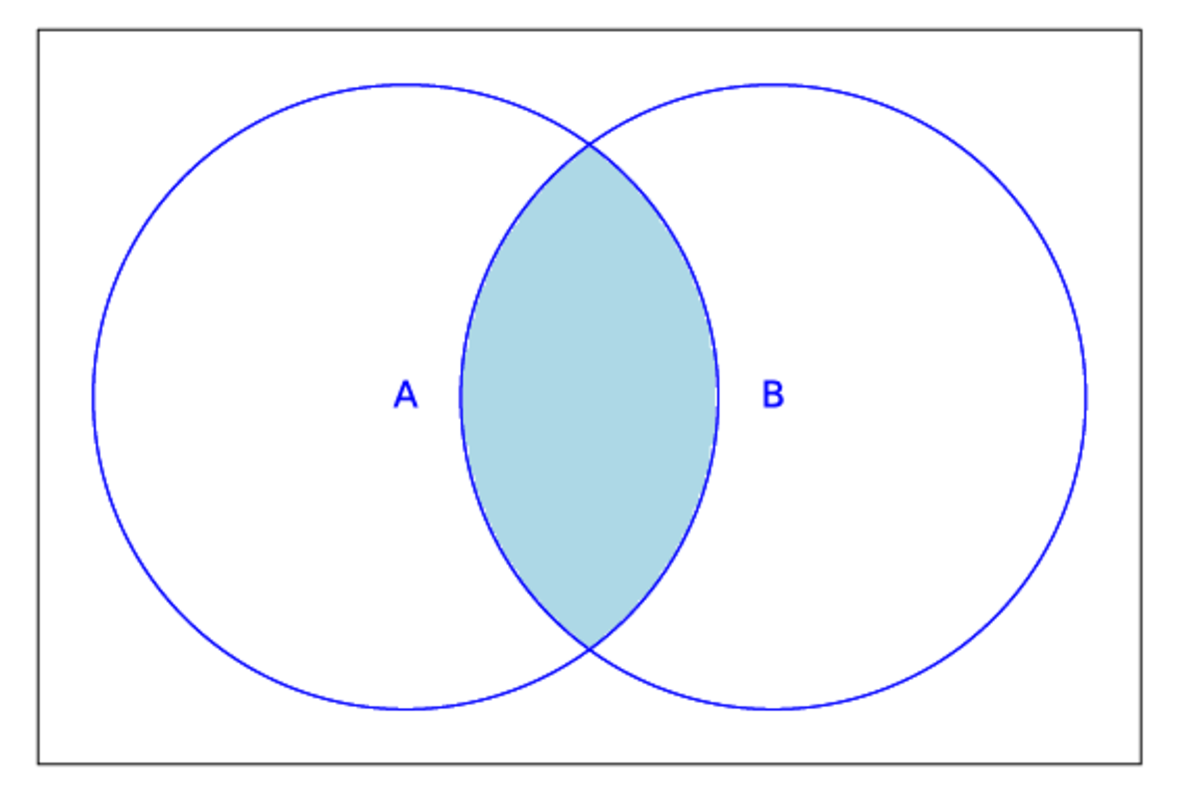
\includegraphics[width=\linewidth]{images/sageplot-venn-intersection.pdf}}%
{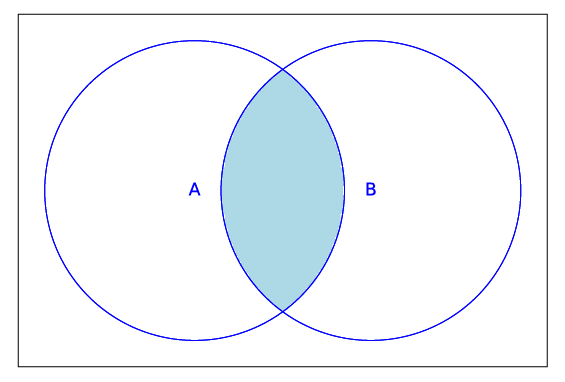
\includegraphics[width=\linewidth]{images/sageplot-venn-intersection.png}}
\end{image}%
\tcblower
\end{figureptx}%
The union \(A \cup  B\) is illustrated in \hyperref[x:figure:venn_diagram_union]{Figure~{\xreffont\ref{x:figure:venn_diagram_union}}}.%
\begin{figureptx}{Venn Diagram for the Union \(A \cup  B\)}{x:figure:venn_diagram_union}{}%
\begin{image}{0.2}{0.6}{0.2}%
\IfFileExists{images/sageplot-venn-union.pdf}%
{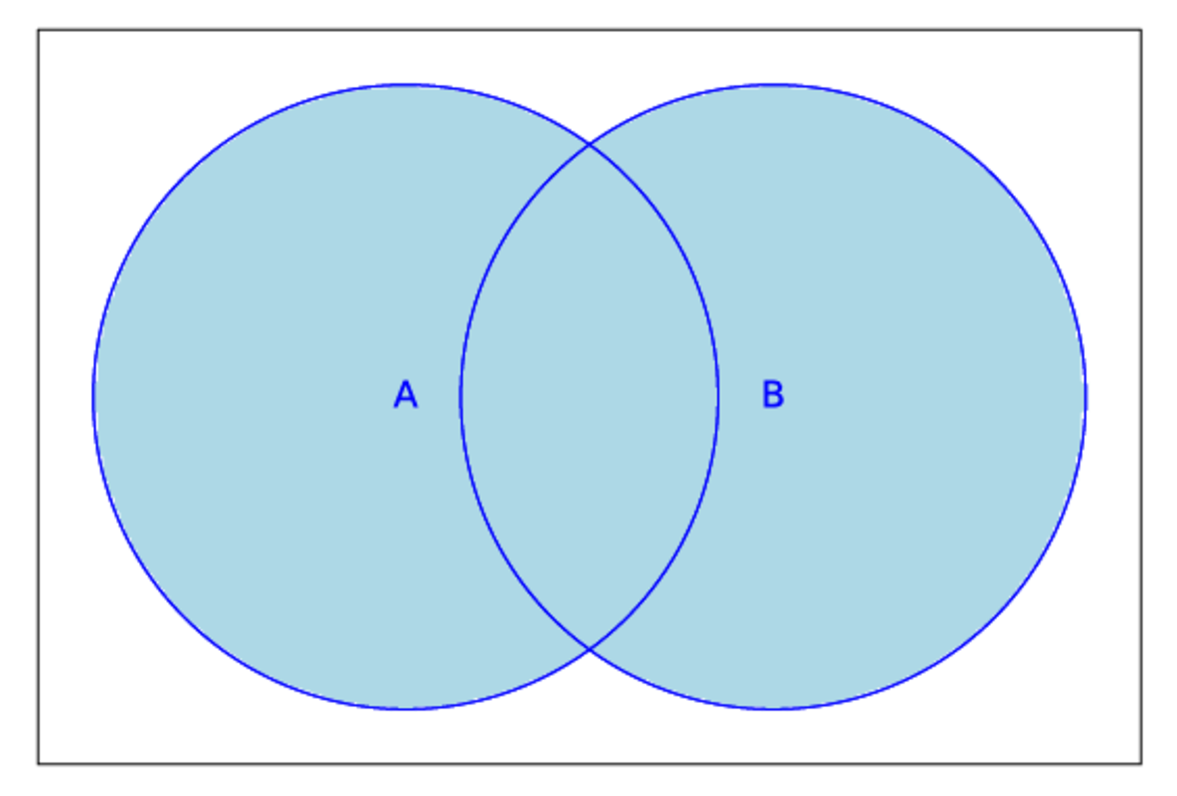
\includegraphics[width=\linewidth]{images/sageplot-venn-union.pdf}}%
{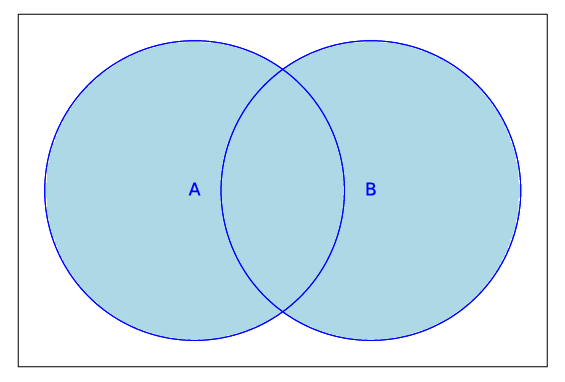
\includegraphics[width=\linewidth]{images/sageplot-venn-union.png}}
\end{image}%
\tcblower
\end{figureptx}%
In a Venn diagram, the region representing \(A \cap  B\) does not appear empty; however, in some instances it will represent the empty set. The same is true for any other region in a Venn diagram.%
\end{example}
\begin{definition}{Complement of a set.}{x:definition:set_complement}%
\index{Complement of a set}%
\label{g:notation:idm40463121216}%
\label{g:notation:idm40470599920}%
Let \(A\) and \(B\) be sets. The complement of \(A\) relative to \(B\) (notation \(B - A\)) is the set of elements that are in \(B\) and not in \(A\). That is, \(B-A=\{x: x\in B \textrm{ and } x\notin A\}\). If \(U\) is the universal set, then \(U-A\) is denoted by \(A^c\) and is called simply the complement of \(A\). \(A^c=\{x\in U : x\notin A\}\).%
\end{definition}
\begin{figureptx}{Venn Diagram for \(B - A\)}{x:figure:venn_diagram_complement1}{}%
\begin{image}{0.2}{0.6}{0.2}%
\IfFileExists{images/sageplot-venn-complement1.pdf}%
{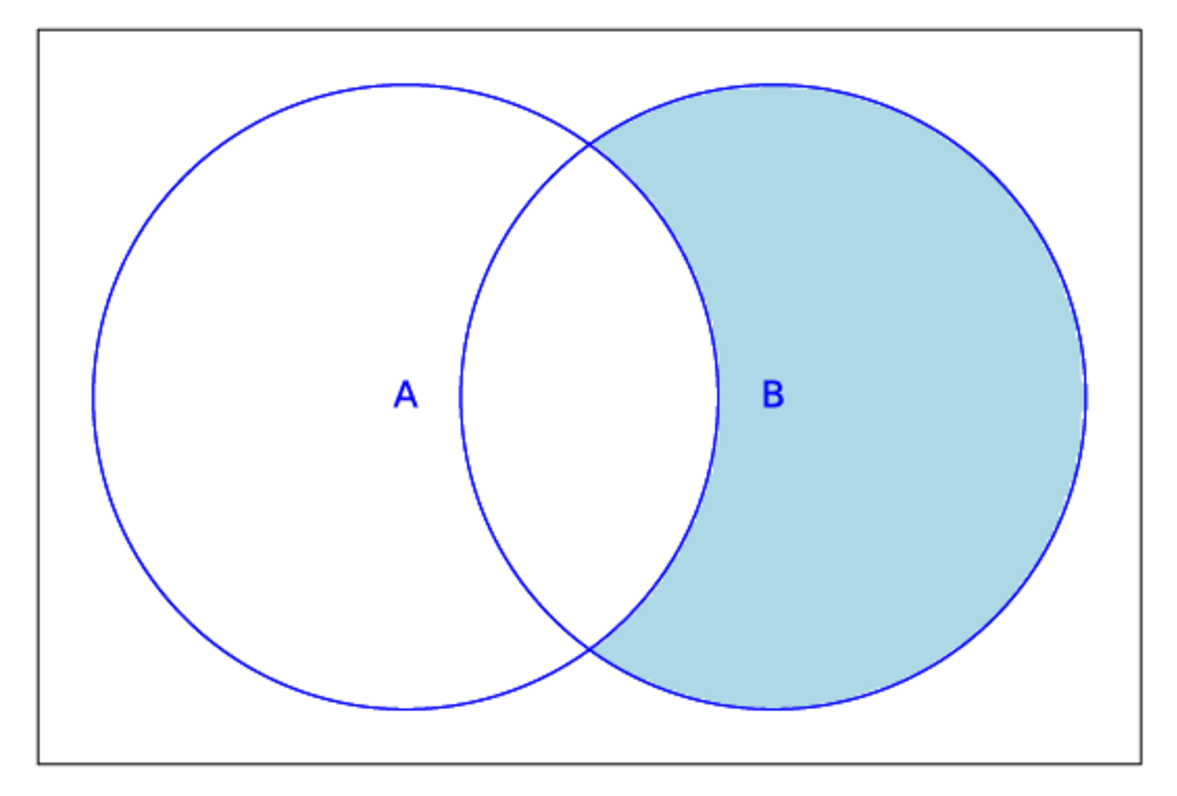
\includegraphics[width=\linewidth]{images/sageplot-venn-complement1.pdf}}%
{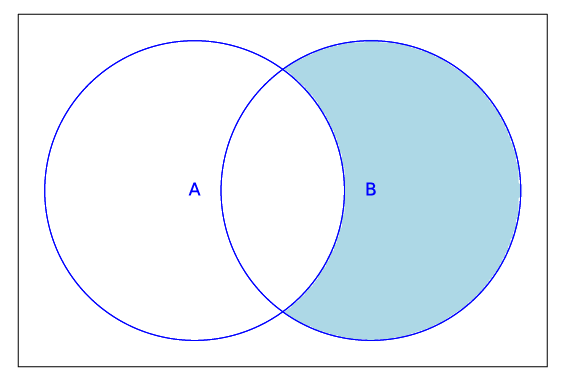
\includegraphics[width=\linewidth]{images/sageplot-venn-complement1.png}}
\end{image}%
\tcblower
\end{figureptx}%
\begin{example}{Some Complements.}{x:example:complements}%
%
\begin{enumerate}[label=(\alph*)]
\item{}Let \(U = \{1,2, 3, \text{...} , 10\}\) and \(A = \{2,4,6,8, 10\}\). Then \(U-A = \{1, 3, 5, 7, 9\}\) and \(A - U= \emptyset\).%
\item{}If \(U = \mathbb{R}\), then the complement of the set of rational numbers is the set of irrational numbers.%
\item{}\(U^c= \emptyset\) and \(\emptyset ^c= U\).%
\item{}The Venn diagram of \(B - A\) is represented in \hyperref[x:figure:venn_diagram_complement1]{Figure~{\xreffont\ref{x:figure:venn_diagram_complement1}}}.%
\item{}The Venn diagram of \(A^c\) is represented in \hyperref[x:figure:venn_diagram_complement2]{Figure~{\xreffont\ref{x:figure:venn_diagram_complement2}}}.%
\item{}If \(B\subseteq A\), then the Venn diagram of \(A- B\) is as shown in \hyperref[x:figure:venn_diagram_complement3]{Figure~{\xreffont\ref{x:figure:venn_diagram_complement3}}}.%
\item{}In the universe of integers, the set of even integers, \(\{\ldots  , - 4,-2, 0, 2, 4,\ldots \}\), has the set of odd integers as its complement.%
\end{enumerate}
%
\begin{figureptx}{Venn Diagram for \(A^{c}\)}{x:figure:venn_diagram_complement2}{}%
\begin{image}{0.2}{0.6}{0.2}%
\IfFileExists{images/sageplot-venn-complement2.pdf}%
{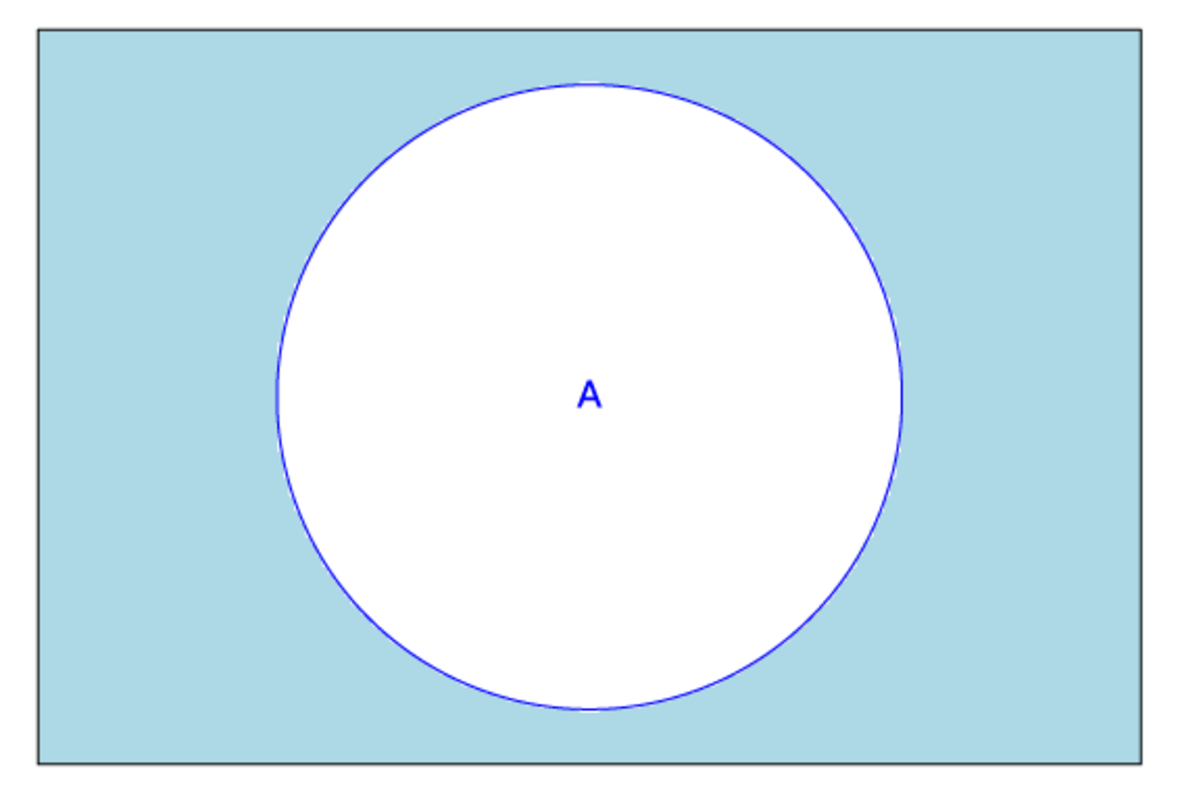
\includegraphics[width=\linewidth]{images/sageplot-venn-complement2.pdf}}%
{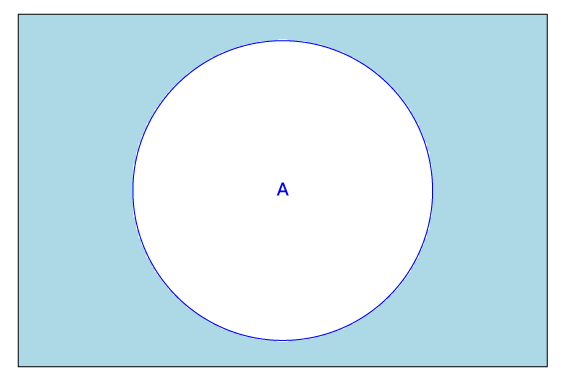
\includegraphics[width=\linewidth]{images/sageplot-venn-complement2.png}}
\end{image}%
\tcblower
\end{figureptx}%
\begin{figureptx}{Venn Diagram for \(A-B\) when \(B\) is a subset of \(A\)}{x:figure:venn_diagram_complement3}{}%
\begin{image}{0.2}{0.6}{0.2}%
\IfFileExists{images/sageplot-venn-complement3.pdf}%
{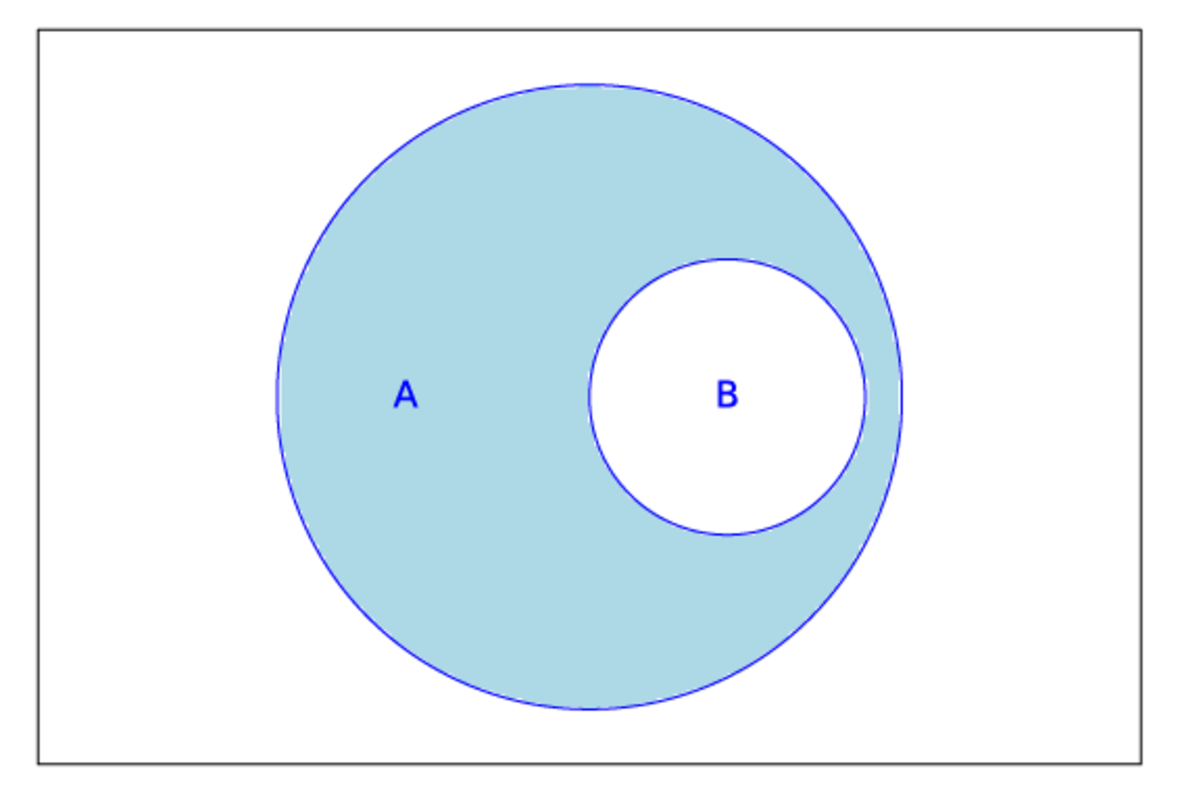
\includegraphics[width=\linewidth]{images/sageplot-venn-complement3.pdf}}%
{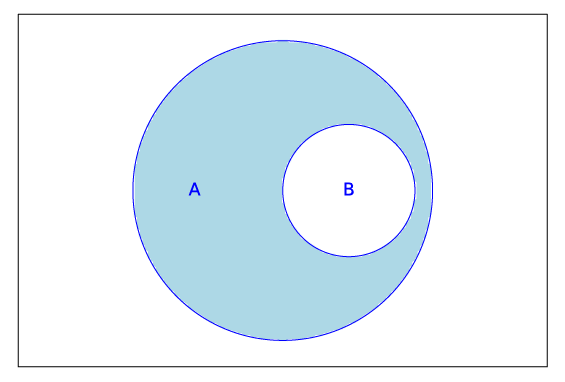
\includegraphics[width=\linewidth]{images/sageplot-venn-complement3.png}}
\end{image}%
\tcblower
\end{figureptx}%
\end{example}
\begin{definition}{Symmetric Difference.}{x:definition:symmetric-difference}%
\index{Symmetric Difference}%
\label{g:notation:idm40486529680}%
Let \(A\) and \(B\) be sets. The symmetric difference of \(A\) and \(B\) (denoted by \(A\oplus B\)) is the set of all elements that are in \(A\) and \(B\) but not in both. That is, \(A \oplus  B = (A \cup  B) - (A \cap  B)\).%
\end{definition}
\begin{example}{Some Symmetric Differences.}{x:example:some_symmetric_differences}%
%
\begin{enumerate}[label=(\alph*)]
\item{}Let \(A = \{1, 3, 8\}\) and \(B = \{2, 4, 8\}\). Then \(A \oplus  B = \{1, 2, 3, 4\}\).%
\item{}\(A \oplus  \emptyset = A\) and \(A \oplus  A = \emptyset\) for any set \(A\).%
\item{}\(\mathbb{R} \oplus  \mathbb{Q}\) is the set of irrational numbers.%
\item{}The Venn diagram of \(A \oplus  B\) is represented in \hyperref[x:figure:venn_diagram_symmetric]{Figure~{\xreffont\ref{x:figure:venn_diagram_symmetric}}}.%
\end{enumerate}
%
\begin{figureptx}{Venn Diagram for the symmetric difference \(A \oplus  B\)}{x:figure:venn_diagram_symmetric}{}%
\begin{image}{0.2}{0.6}{0.2}%
\IfFileExists{images/sageplot-venn-symmetric.pdf}%
{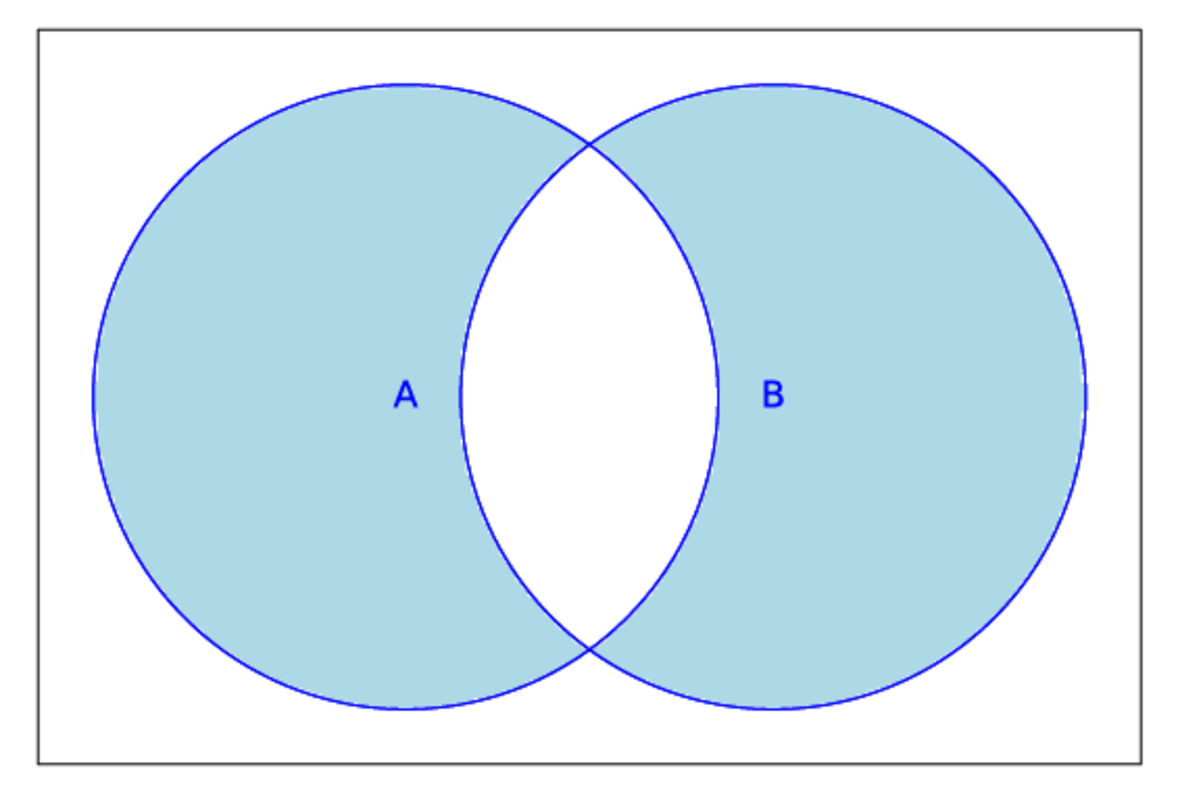
\includegraphics[width=\linewidth]{images/sageplot-venn-symmetric.pdf}}%
{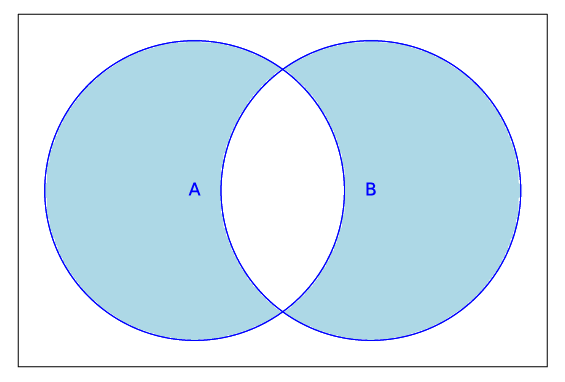
\includegraphics[width=\linewidth]{images/sageplot-venn-symmetric.png}}
\end{image}%
\tcblower
\end{figureptx}%
\end{example}
\end{subsectionptx}
%
%
\typeout{************************************************}
\typeout{Subsection 1.2.3 SageMath Note: Sets}
\typeout{************************************************}
%
\begin{subsectionptx}{SageMath Note: Sets}{}{SageMath Note: Sets}{}{}{x:subsection:Sage_Note_Sets-1-2}
\index{SageMath Note!Sets}%
To work with sets in Sage, a set is an expression of the form  Set(\emph{list}).  By wrapping a list with \mono{Set( )}, the order of elements appearing in the list and their duplication are ignored.  For example, L1 and L2 are two different lists, but notice how as sets they are considered equal:%
\begin{sageinput}
L1=[3,6,9,0,3]
L2=[9,6,3,0,9]
[L1==L2, Set(L1)==Set(L2) ]
\end{sageinput}
\begin{sageoutput}
[False, True]
\end{sageoutput}
The standard set operations are all methods and\slash{}or functions that can act on Sage sets. \emph{You need to evaluate the following cell to use the subsequent cell.}%
\begin{sageinput}
A=Set(srange(5,50,5))
B=Set(srange(6,50,6))
[A,B]
\end{sageinput}
\begin{sageoutput}
[{35, 5, 40, 10, 45, 15, 20, 25, 30}, {36, 6, 42, 12, 48, 18, 24, 30}]
\end{sageoutput}
We can test membership, asking whether 10 is in each of the sets:%
\begin{sageinput}
[10 in A, 10 in B]
\end{sageinput}
\begin{sageoutput}
[True, False]
\end{sageoutput}
The ampersand is used for the intersection of sets.  Change it to the vertical bar, \textbar{}, for union.%
\begin{sageinput}
A & B
\end{sageinput}
\begin{sageoutput}
{30}
\end{sageoutput}
Symmetric difference and set complement are defined as ``methods'' in Sage. Here is how to compute the symmetric difference of \(A\)  with  \(B\), followed by their differences.%
\begin{sageinput}
[A.symmetric_difference(B),A.difference(B),B.difference(A)]
\end{sageinput}
\begin{sageoutput}
[{35, 36, 5, 6, 40, 42, 12, 45, 15, 48, 18, 20, 24, 25, 10},
 {35, 5, 40, 10, 45, 15, 20, 25},
 {48, 18, 36, 6, 24, 42, 12}]
\end{sageoutput}
\end{subsectionptx}
%
%
\typeout{************************************************}
\typeout{Exercises 1.2.4 Exercises}
\typeout{************************************************}
%
\begin{exercises-subsection}{Exercises}{}{Exercises}{}{}{x:exercises:exercises-1-2}
\begin{divisionexercise}{1}{}{}{g:exercise:idm40462533632}%
Let \(A = \{0, 2, 3\}\), \(B = \{2, 3\}\), \(C = \{1, 5, 9\}\), and let the universal set be \(U = \{0, 1, 2, . . . , 9\}\). Determine:%
\begin{multicols}{3}
\begin{enumerate}[label=(\alph*)]
\item{}\(A \cap  B\)%
\item{}\(A \cup  B\)%
\item{}\(B \cup  A\)%
\item{}\(A \cup  C\)%
\item{}\(A - B\)%
\item{}\(B - A\)%
\item{}\(A^c\)%
\item{}\(C^c\)%
\item{}\(A\cap C\)%
\item{}\(A\oplus B\)%
\end{enumerate}
\end{multicols}
%
\end{divisionexercise}%
\begin{divisionexercise}{2}{}{}{g:exercise:idm40486503232}%
Let \(A\), \(B\), and \(C\) be as in Exercise 1, let \(D = \{3, 2\}\), and let \(E = \{2, 3, 2\}\). Determine which of the following are true. Give reasons for your decisions.%
\begin{multicols}{2}
\begin{enumerate}[label=(\alph*)]
\item{}\(A = B\)%
\item{}\(B = C\)%
\item{}\(B = D\)%
\item{}\(E=D\)%
\item{}\(A\cap B = B\cap A\)%
\item{}\(A \cup  B = B \cup  A\)%
\item{}\(A-B = B-A\)%
\item{}\(A \oplus  B = B \oplus  A\)%
\end{enumerate}
\end{multicols}
%
\end{divisionexercise}%
\begin{divisionexercise}{3}{}{}{g:exercise:idm40471421920}%
Let \(U= \{1, 2, 3, . . . , 9\}\). Give examples of sets \(A\), \(B\), and \(C\) for which:%
\begin{multicols}{2}
\begin{enumerate}[label=(\alph*)]
\item{}\(A\cap (B\cap C)=(A\cap B)\cap C\)%
\item{}\(A\cap (B\cup C)=(A\cap B)\cup (A\cap C)\)%
\item{}\((A \cup  B)^c= A^c\cap B^c\)%
\item{}\(A \cup  A^c = U\)%
\item{}\(A \subseteq A\cup B\)%
\item{}\(A\cap B \subseteq A\)%
\end{enumerate}
\end{multicols}
%
\end{divisionexercise}%
\begin{divisionexercise}{4}{}{}{g:exercise:idm40462991056}%
Let \(U= \{1, 2, 3, . . . , 9\}\). Give examples to illustrate the following facts:%
\begin{enumerate}[label=(\alph*)]
\item{}If \(A \subseteq  B\) and \(B \subseteq C\), then \(A\subseteq C\).%
\item{}There are sets \(A\) and \(B\) such that \(A - B \neq  B - A\)%
\item{}If \(U = A\cup  B\) and \(A \cap  B = \emptyset\), it always follows that \(A = U - B\).%
\end{enumerate}
%
\end{divisionexercise}%
\begin{divisionexercise}{5}{}{}{g:exercise:idm40462984976}%
What can you say about \(A\) if \(U = \{1, 2, 3, 4, 5\}\), \(B = \{2, 3\}\), and (separately)%
\begin{enumerate}[label=(\alph*)]
\item{}\(A \cup B = \{1, 2, 3,4\}\)%
\item{}\(A \cap  B = \{2\}\)%
\item{}\(A \oplus  B = \{3, 4, 5\}\)%
\end{enumerate}
%
\end{divisionexercise}%
\begin{divisionexercise}{6}{}{}{g:exercise:idm40462977904}%
Suppose that \(U\) is an infinite universal set, and \(A\) and \(B\) are infinite subsets of \(U\). Answer the following questions with a brief explanation.%
\par
%
\begin{enumerate}[label=(\alph*)]
\item{}Must \(A^c\) be finite?%
\item{}Must \(A\cup B\) be infinite?%
\item{}Must \(A\cap B\) be infinite?%
\end{enumerate}
%
\end{divisionexercise}%
\begin{divisionexercise}{7}{}{}{g:exercise:idm40462972848}%
Given that \(U\) = all students at a university, \(D\) = day students, \(M\) = mathematics majors, and \(G\) = graduate students. Draw Venn diagrams illustrating this situation and shade in the following sets:%
\par
%
\begin{multicols}{2}
\begin{enumerate}[label=(\alph*)]
\item{}evening students%
\item{}undergraduate mathematics majors%
\item{}non-math graduate students%
\item{}non-math undergraduate students%
\end{enumerate}
\end{multicols}
%
\end{divisionexercise}%
\begin{divisionexercise}{8}{}{}{g:exercise:idm40462966656}%
Let the sets \(D\), \(M\), \(G\), and \(U\) be as in exercise 7.  Let \(\lvert U \rvert  = 16,000\), \(\lvert D \rvert = 9,000\), \(|M|=
300\), and \(\lvert G \rvert = 1,000\). Also assume that the number of day students who are mathematics majors is 250, 50 of whom are graduate students, that there are 95 graduate mathematics majors, and that the total number of day graduate students is 700. Determine the number of students who are:%
\begin{multicols}{2}
\begin{enumerate}[label=(\alph*)]
\item{}evening students%
\item{}nonmathematics majors%
\item{}undergraduates (day or evening)%
\item{}day graduate nonmathematics majors%
\item{}evening graduate students%
\item{}evening graduate mathematics majors%
\item{}evening undergraduate nonmathematics majors%
\end{enumerate}
\end{multicols}
%
\end{divisionexercise}%
\end{exercises-subsection}
\end{sectionptx}
%
%
\typeout{************************************************}
\typeout{Section 1.3 Cartesian Products and Power Sets}
\typeout{************************************************}
%
\begin{sectionptx}{Cartesian Products and Power Sets}{}{Cartesian Products and Power Sets}{}{}{x:section:s-cartesian_Products_and_Power_Sets}
%
%
\typeout{************************************************}
\typeout{Subsection 1.3.1 Cartesian Products}
\typeout{************************************************}
%
\begin{subsectionptx}{Cartesian Products}{}{Cartesian Products}{}{}{x:subsection:Cartesian-products}
\begin{definition}{Cartesian Product.}{x:definition:cartesian-product}%
\index{Cartesian Product}%
\label{g:notation:idm40462957296}%
Let \(A\) and \(B\) be sets. The Cartesian product of \(A\) and \(B\), denoted by \(A\times B\), is defined as follows: \(A\times B = \{(a, b) \mid a \in  A \quad\textrm{and}\quad b \in  B\}\), that is, \(A\times B\) is the set of all possible ordered pairs whose first component comes from \(A\) and whose second component comes from \(B\).%
\end{definition}
\begin{example}{Some Cartesian Products.}{g:example:idm40462955632}%
Notation in mathematics is often developed for good reason. In this case, a few examples will make clear why the symbol \(\times\) is used for Cartesian products.%
\par
%
\begin{itemize}[label=\textbullet]
\item{}Let \(A = \{1, 2, 3\}\) and \(B = \{4, 5\}\). Then \(A \times  B = \{(1, 4), (1, 5), (2, 4), (2, 5), (3, 4), (3, 5)\}\). Note that \(|A \times B| = 6 = \lvert A \rvert  \times  \lvert B \rvert \).%
\item{}\(A \times  A = \{(1, 1), (1, 2), (1, 3), (2, 1), (2, 2), (2, 3), (3, 1), (3, 2), (3, 3)\}\). Note that \(|A \times  A| = 9 = {\lvert A \rvert}^2\).%
\end{itemize}
%
\end{example}
These two examples illustrate the general rule that if \(A\) and \(B\) are finite sets, then \(\lvert A \times B \rvert = \lvert A \rvert  \times  \lvert B \rvert \).%
\par
We can define the Cartesian product of three (or more) sets similarly. For example, \(A \times  B \times  C = \{(a, b, c):a \in  A, b \in  B, c \in C\}\).%
\par
It is common to use exponents if the sets in a Cartesian product are the same:%
\begin{equation*}
A^2= A \times  A
\end{equation*}
%
\begin{equation*}
A^3=A \times A \times A
\end{equation*}
and in general,%
\begin{equation*}
A^n =  \underset{n \textrm{ factors}}{\underline{A \times A \times \ldots \times A}}\text{.}
\end{equation*}
%
\end{subsectionptx}
%
%
\typeout{************************************************}
\typeout{Subsection 1.3.2 Power Sets}
\typeout{************************************************}
%
\begin{subsectionptx}{Power Sets}{}{Power Sets}{}{}{x:subsection:power-sets}
\begin{definition}{Power Set.}{x:definition:power-set}%
\index{Power Set}%
\label{g:notation:idm40462942256}%
If \(A\) is any set, the power set of \(A\) is the set of all subsets of \(A\), denoted \(\mathcal{P}(A)\).%
\end{definition}
The two extreme cases, the empty set and all of \(A\), are both included in \(\mathcal{P}(A)\).%
\begin{example}{Some Power Sets.}{x:example:Some_Power_Sets}%
%
\begin{itemize}[label=\textbullet]
\item{}\(\mathcal{P}(\emptyset )=\{\emptyset \}\)%
\item{}\(\mathcal{P}(\{1\}) = \{\emptyset , \{1\}\}\)%
\item{}\(\mathcal{P}(\{1,2\}) = \{\emptyset , \{1\}, \{2\}, \{1, 2\}\}\).%
\end{itemize}
%
\par
We will leave it to you to guess at a general formula for the number of elements in the power set of a finite set. In Chapter 2, we will discuss counting rules that will help us derive this formula.%
\end{example}
\end{subsectionptx}
%
%
\typeout{************************************************}
\typeout{Subsection 1.3.3 SageMath Note: Cartesian Products and Power Sets}
\typeout{************************************************}
%
\begin{subsectionptx}{SageMath Note: Cartesian Products and Power Sets}{}{SageMath Note: Cartesian Products and Power Sets}{}{}{x:subsection:Sage_Note_Sets-1-3}
\index{SageMath Note!Cartesian Products and Power Sets}%
Here is a simple example of a cartesian product of two sets:%
\begin{sageinput}
A=Set([0,1,2])
B=Set(['a','b'])
P=cartesian_product([A,B]);P
\end{sageinput}
\begin{sageoutput}
The Cartesian product of ({0, 1, 2}, {'a', 'b'})
\end{sageoutput}
Here is the cardinality of the cartesian product.%
\begin{sageinput}
P.cardinality()
\end{sageinput}
\begin{sageoutput}
6
\end{sageoutput}
The power set of a set is an iterable, as you can see from the output of this next cell%
\begin{sageinput}
U=Set([0,1,2,3])
subsets(U)
\end{sageinput}
\begin{sageoutput}
<generator object powerset at 0x7fec5ffd33c0>
\end{sageoutput}
You can iterate over a powerset. Here is a trivial example.%
\begin{sageinput}
for a in subsets(U):
    print(str(a)+ " has " +str(len(a))+" elements.")
\end{sageinput}
\begin{sageoutput}
[] has 0 elements.
[0] has 1 elements.
[1] has 1 elements.
[0, 1] has 2 elements.
[2] has 1 elements.
[0, 2] has 2 elements.
[1, 2] has 2 elements.
[0, 1, 2] has 3 elements.
[3] has 1 elements.
[0, 3] has 2 elements.
[1, 3] has 2 elements.
[0, 1, 3] has 3 elements.
[2, 3] has 2 elements.
[0, 2, 3] has 3 elements.
[1, 2, 3] has 3 elements.
[0, 1, 2, 3] has 4 elements.
\end{sageoutput}
\end{subsectionptx}
%
%
\typeout{************************************************}
\typeout{Exercises 1.3.4 Exercises}
\typeout{************************************************}
%
\begin{exercises-subsection}{Exercises}{}{Exercises}{}{}{x:exercises:exercises-1-3}
\begin{divisionexercise}{1}{}{}{g:exercise:idm40462928288}%
Let \(A = \{0, 2, 3\}\), \(B = \{2, 3\}\), \(C = \{1, 4\}\), and let the universal set be \(U = \{0, 1, 2, 3, 4\}\). List the elements of%
\par
%
\begin{multicols}{2}
\begin{enumerate}[label=(\alph*)]
\item{}\(A \times B\)%
\item{}\(B \times  A\)%
\item{}\(A \times B\times C\)%
\item{}\(U \times \emptyset\)%
\item{}\(A \times  A^c\)%
\item{}\(B^2\)%
\item{}\(B^3\)%
\item{}\(B\times \mathcal{P}(B)\)%
\end{enumerate}
\end{multicols}
%
\end{divisionexercise}%
\begin{divisionexercise}{2}{}{}{g:exercise:idm40462914992}%
Suppose that you are about to flip a coin and then roll a die. Let \(A = \{HEADS, TAILS\}\) and  \(B = \{1, 2, 3, 4, 5, 6\}\).%
\par
%
\begin{enumerate}[label=(\alph*)]
\item{}What is \(|A \times  B|\)?%
\item{}How could you interpret the set \(A \times  B\) ?%
\end{enumerate}
%
\end{divisionexercise}%
\begin{divisionexercise}{3}{}{}{g:exercise:idm40462911472}%
List all two-element sets in \(\mathcal{P}(\{a,b,c,d\})\)%
\end{divisionexercise}%
\begin{divisionexercise}{4}{}{}{g:exercise:idm40462909840}%
List all three-element sets in \(\mathcal{P}(\{a, b, c,d\})\).%
\end{divisionexercise}%
\begin{divisionexercise}{5}{}{}{g:exercise:idm40462908720}%
How many singleton (one-element) sets are there in \(\mathcal{P}(A)\) if \(\lvert A \rvert =n\) ?%
\end{divisionexercise}%
\begin{divisionexercise}{6}{}{}{g:exercise:idm40462906448}%
A person has four coins in his pocket: a penny, a nickel, a dime, and a quarter. How many different sums of money can he take out if he removes 3 coins at a time?%
\end{divisionexercise}%
\begin{divisionexercise}{7}{}{}{g:exercise:idm40462905536}%
Let \(A = \{+,-\}\) and \(B = \{00, 01, 10, 11\}\).%
\par
%
\begin{enumerate}[label=(\alph*)]
\item{}List the elements of \(A \times  B\)%
\item{}How many elements do \(A ^4\) and \((A \times B)^3\) have?%
\end{enumerate}
%
\end{divisionexercise}%
\begin{divisionexercise}{8}{}{}{g:exercise:idm40462899744}%
Let \(A = \{\bullet,\square ,\otimes \}\) and \(B = \{\square ,\ominus ,\bullet\}\).%
\par
%
\begin{enumerate}[label=(\alph*)]
\item{}List the elements of \(A \times  B\) and \(B \times  A\). The parentheses and comma in an ordered pair are not necessary in cases such as this where the elements of each set are individual symbols.%
\item{}Identify the intersection of \(A \times  B\) and \(B \times  A\) for the case above, and then guess at a general rule for the intersection of \(A \times  B\) and \(B \times  A\), where \(A\) and \(B\) are any two sets.%
\end{enumerate}
%
\end{divisionexercise}%
\begin{divisionexercise}{9}{}{}{g:exercise:idm40462896208}%
Let \(A\) and \(B\) be nonempty sets. When are \(A \times  B\) and \(B \times  A\) equal?%
\end{divisionexercise}%
\end{exercises-subsection}
\end{sectionptx}
%
%
\typeout{************************************************}
\typeout{Section 1.4 Binary Representation of Positive Integers}
\typeout{************************************************}
%
\begin{sectionptx}{Binary Representation of Positive Integers}{}{Binary Representation of Positive Integers}{}{}{x:section:s-binary_Representation_of_Positive_Integers}
\index{Binary Representation}%
%
%
\typeout{************************************************}
\typeout{Subsection 1.4.1 Grouping by Twos}
\typeout{************************************************}
%
\begin{subsectionptx}{Grouping by Twos}{}{Grouping by Twos}{}{}{x:subsection:ss-grouping-by-twos}
Recall that the set of positive integers, \(\mathbb{P}\), is \(\{1, 2, 3, . . . \}\). Positive integers are naturally used to count things. There are many ways to count and many ways to record, or represent, the results of counting. For example, if we wanted to count five hundred twenty-three apples, we might group the apples by tens. There would be fifty-two groups of ten with three single apples left over. The fifty-two groups of ten could be put into five groups of ten tens (hundreds), with two tens left over. The five hundreds, two tens, and three units is recorded as 523. This system of counting is called the base ten positional system, or decimal system. It is quite natural for us to do grouping by tens, hundreds, thousands, \(\dots\) since it is the method that all of us use in everyday life.%
\par
The term positional refers to the fact that each digit in the decimal representation of a number has a significance based on its position. Of course this means that rearranging digits will change the number being described. You may have learned of numeration systems in which the position of symbols does not have any significance (e.g., the ancient Egyptian system). Most of these systems are merely curiosities to us now.%
\par
The binary number system differs from the decimal number system in that units are grouped by twos, fours, eights, etc. That is, the group sizes are powers of two instead of powers of ten. For example, twenty-three can be grouped into eleven groups of two with one left over. The eleven twos can be grouped into five groups of four with one group of two left over. Continuing along the same lines, we find that twenty-three can be described as one sixteen, zero eights, one four, one two, and one one, which is abbreviated \(10111_{\textrm{two}}\), or simply \(10111\) if the context is clear.%
\end{subsectionptx}
%
%
\typeout{************************************************}
\typeout{Subsection 1.4.2 A Conversion Algorithm}
\typeout{************************************************}
%
\begin{subsectionptx}{A Conversion Algorithm}{}{A Conversion Algorithm}{}{}{x:subsection:ss-conversion-algorithm}
The process that we used to determine the binary representation of \(23\) can be described in general terms to determine the binary representation of any positive integer \(n\). A general description of a process such as this one is called an algorithm. Since this is the first algorithm in the book, we will first write it out using less formal language than usual, and then introduce some ``algorithmic notation.''  If you are unfamiliar with algorithms, we refer you to \hyperref[x:section:app-alg1]{Section~{\xreffont\ref{x:section:app-alg1}}}%
\par
%
\begin{enumerate}[label=(\arabic*)]
\item{}Start with an empty list of bits.%
\item{}Step Two: Assign the variable \(k\) the value \(n\).%
\item{}Step Three: While \(k\)'s value is positive, continue performing the following three steps until \(k\) becomes zero and then stop.%
\par
%
\begin{enumerate}[label=(\alph*)]
\item{}divide \(k\) by 2, obtaining a quotient \(q\) (often denoted \(k \textrm{ div } 2\)) and a remainder \(r\) (denoted \((k \bmod 2)\)).%
\item{}attach \(r\) to the left-hand side of the list of bits.%
\item{}assign the variable \(k\) the value \(q\).%
\end{enumerate}
%
\end{enumerate}
%
\begin{example}{An example of conversion to binary.}{x:example:An_example_of_conversion_to_binary}%
To determine the binary representation of 41 we take the following steps:%
\par
%
\begin{itemize}[label=\textbullet]
\item{}\(41 = 2 \times  20+ 1 \quad List = 1 \)%
\item{}\(20 = 2 \times  10+0 \quad List = 01 \)%
\item{}\(10 = 2\times 5 + 0 \quad List = 001 \)%
\item{}\(5 =\text2\times  2+ 1 \quad List =1001\)%
\item{}\(2 =2\times  1+ 0 \quad List = 01001 \)%
\item{}\(1 =\text2 \times 0\text+1  \quad List = 101001\)%
\end{itemize}
%
\par
Therefore, \(41=101001_{\textrm{two}}\)%
\end{example}
The notation that we will use to describe this algorithm and all others is called pseudocode, an informal variation of the instructions that are commonly used in many computer languages. Read the following description carefully, comparing it with the informal description above. Appendix B, which contains a general discussion of the components of the algorithms in this book, should clear up any lingering questions. Anything after \slash{}\slash{} are comments.%
\begin{algorithm}{Binary Conversion Algorithm.}{}{x:algorithm:binary-conversion-algorithm}%
\index{Binary Conversion Algorithm}%
An algorithm for determining the binary representation of a positive integer.%
\par
Input: a positive integer n.%
\par
Output: the binary representation of n in the form of a list of bits, with units bit last, twos bit next to last, etc.%
\par
%
\begin{enumerate}[label=(\arabic*)]
\item{}k := n \(\qquad  \)     \slash{}\slash{}initialize k%
\item{}L := \textbraceleft{} \textbraceright{} \(\qquad  \)   \slash{}\slash{}initialize L to an empty list%
\item{}While k \textgreater{} 0 do%
\par
%
\begin{enumerate}[label=(\alph*)]
\item{}q := k div 2		\(\qquad  \)	\slash{}\slash{}divide k by 2%
\item{}r:= k mod 2%
\item{}L: = prepend r to L \(\qquad  \) \slash{}\slash{}add r to the front of L%
\item{}k:= q   			\(\qquad  \)	\slash{}\slash{}reassign k%
\end{enumerate}
%
\end{enumerate}
%
\end{algorithm}
Here is a Sage version of the algorithm with two alterations. It outputs the binary representation as a string, and it handles all integers, not just positive ones.%
\begin{sageinput}
def binary_rep(n):
    if n==0:
        return '0'
    else:
        k=abs(n)
        s=''
        while k>0:
            s=str(k%2)+s
            k=k//2
        if n < 0:
            s='-'+s
        return s
 
binary_rep(41)
\end{sageinput}
\begin{sageoutput}
'101001'
\end{sageoutput}
Now that you've read this section, you should get this joke.%
\begin{figureptx}{With permission from Randall Munroe}{x:figure:onetoten}{}%
\begin{image}{0.18}{0.64}{0.18}%
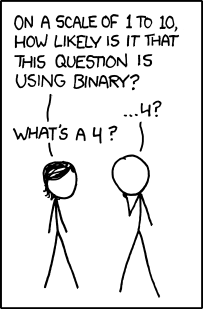
\includegraphics[width=\linewidth]{images/1_to_10.png}
\end{image}%
\tcblower
\end{figureptx}%
\end{subsectionptx}
%
%
\typeout{************************************************}
\typeout{Exercises 1.4.3 Exercises}
\typeout{************************************************}
%
\begin{exercises-subsection}{Exercises}{}{Exercises}{}{}{x:exercises:exercises-1-4}
\begin{divisionexercise}{1}{}{}{g:exercise:idm40465054064}%
Find the binary representation of each of the following positive integers by working through the algorithm by hand.  You can check your answer using the sage cell above.%
\par
%
\begin{multicols}{2}
\begin{enumerate}[label=(\alph*)]
\item{}31%
\item{}32%
\item{}10%
\item{}100%
\end{enumerate}
\end{multicols}
%
\end{divisionexercise}%
\begin{divisionexercise}{2}{}{}{g:exercise:idm40465047520}%
Find the binary representation of each of the following positive integers by working through the algorithm by hand.  You can check your answer using the sage cell above.%
\par
%
\begin{multicols}{2}
\begin{enumerate}[label=(\alph*)]
\item{}64%
\item{}67%
\item{}28%
\item{}256%
\end{enumerate}
\end{multicols}
%
\end{divisionexercise}%
\begin{divisionexercise}{3}{}{}{g:exercise:idm40465044368}%
What positive integers have the following binary representations?%
\par
%
\begin{multicols}{2}
\begin{enumerate}[label=(\alph*)]
\item{}10010%
\item{}10011%
\item{}101010%
\item{}10011110000%
\end{enumerate}
\end{multicols}
%
\end{divisionexercise}%
\begin{divisionexercise}{4}{}{}{g:exercise:idm40465038000}%
What positive integers have the following binary representations?%
\begin{multicols}{2}
\begin{enumerate}[label=(\alph*)]
\item{}100001%
\item{}1001001%
\item{}1000000000%
\item{}1001110000%
\end{enumerate}
\end{multicols}
%
\end{divisionexercise}%
\begin{divisionexercise}{5}{}{}{g:exercise:idm40465035152}%
The number of bits in the binary representations of integers increases by one as the numbers double.  Using this fact, determine how many bits the binary representations of the following decimal numbers have without actually doing the full conversion.%
\begin{multicols}{4}
\begin{enumerate}[label=(\alph*)]
\item{}2017%
\item{}4000%
\item{}4500%
\item{}\(2^{50}\)%
\end{enumerate}
\end{multicols}
%
\end{divisionexercise}%
\begin{divisionexercise}{6}{}{}{g:exercise:idm40465026624}%
Let \(m\) be a positive integer with \(n\)-bit binary representation: \(a_{n-1}a_{n-2}\cdots  a_1a_0\) with \(a_{n-1}=1\) What are the smallest and largest values that \(m\) could have?%
\end{divisionexercise}%
\begin{divisionexercise}{7}{}{}{g:exercise:idm40465026016}%
If a positive integer is a multiple of 100, we can identify this fact from its decimal representation, since it will end with two zeros. What can you say about a positive integer if its binary representation ends with two zeros? What if it ends in \(k\) zeros?%
\end{divisionexercise}%
\begin{divisionexercise}{8}{}{}{g:exercise:idm40465021296}%
Can a multiple of ten be easily identified from its binary representation?%
\end{divisionexercise}%
\end{exercises-subsection}
\end{sectionptx}
%
%
\typeout{************************************************}
\typeout{Section 1.5 Summation Notation and Generalizations}
\typeout{************************************************}
%
\begin{sectionptx}{Summation Notation and Generalizations}{}{Summation Notation and Generalizations}{}{}{x:section:s-summation_Notation_and_Generalizations}
\index{Summation Notation and Generalizations}%
%
%
\typeout{************************************************}
\typeout{Subsection 1.5.1 Sums}
\typeout{************************************************}
%
\begin{subsectionptx}{Sums}{}{Sums}{}{}{x:subsection:ss-sums}
Most operations such as addition of numbers are introduced as binary operations. That is, we are taught that two numbers may be added together to give us a single number. Before long, we run into situations where more than two numbers are to be added. For example, if four numbers, \(a_1\), \(a_2\), \(a_3\), and \(a_4\) are to be added, their sum may be written down in several ways, such as\(\) \(((a_1+a_2)+a_3)+a_4\) or \(\left(a_1+a_2\right)+\left(a_3+a_4\right)\). In the first expression, the first two numbers are added, the result is added to the third number, and that result is added to the fourth number. In the second expression the first two numbers and the last two numbers are added and the results of these additions are added. Of course, we know that the final results will be the same. This is due to the fact that addition of numbers is an associative operation. For such operations, there is no need to describe how more than two objects will be operated on. A sum of numbers such as \(a_1+a_2+a_3+a_4\) is called a series and is often written \(\sum_{k=1}^4 a_k\) in what is called \emph{summation notation}.%
\par
We first recall some basic facts about series that you probably have seen before. A more formal treatment of sequences and series is covered in Chapter 8. The purpose here is to give the reader a working knowledge of summation notation and to carry this notation through to intersection and union of sets and other mathematical operations.%
\par
A \emph{finite series} is an expression such as \(a_1+a_2+a_3 +\dots +a_n=\sum_{k=1}^{n} a_k\)%
\par
In the expression \(\sum_{k=1}^{n} a_k\):%
\par
%
\begin{itemize}[label=\textbullet]
\item{}The variable \(k\) is referred to as the \emph{index}, or the index of summation.%
\item{}The expression \(a_k\) is the \emph{general term} of the series. It defines the numbers that are being added together in the series.%
\item{}The value of \(k\) below the summation symbol is the \emph{initial index} and the value above the summation symbol is the \emph{terminal index}.%
\item{}It is understood that the series is a sum of the general terms where the index start with the initial index and increases by one up to and including the terminal index.%
\end{itemize}
%
\begin{example}{Some finite series.}{x:example:some_finite_series}%
%
\begin{enumerate}[label=(\alph*)]
\item{}\(\sum_{i=1}^4 a_i= a_1+ a_2+a_3+a_4\)%
\item{}\(\sum_{k=0}^5 b_k=b_0+b_1+b_2+b_3+b_4+b_5\)%
\item{}\(\sum_{i=-2}^2 c_i=c_{-2}+c_{-1}+c_0+c_1+c_2\)%
\end{enumerate}
%
\end{example}
\begin{example}{More finite series.}{x:example:more_finite_series}%
If the general terms in a series are more specific, the sum can often be simplified. For example,%
\par
%
\begin{enumerate}[label=(\alph*)]
\item{}\(\sum_{i=1}^4 i^2=1^2+2^2+3^2+4^2=30\)%
\item{}%
\begin{equation*}
\begin{split}
\sum_{i=1}^5 (2i-1)&=(2\cdot 1-1)+(2\cdot 2-1)+(2\cdot 3-1)+(2\cdot 4-1)+(2\cdot 5-1)\\
& =1+3+5+7+9\\
& =25\\
\end{split}\text{.}
\end{equation*}
%
\end{enumerate}
%
\end{example}
\end{subsectionptx}
%
%
\typeout{************************************************}
\typeout{Subsection 1.5.2 Generalizations}
\typeout{************************************************}
%
\begin{subsectionptx}{Generalizations}{}{Generalizations}{}{}{x:subsection:ss-generalizations}
Summation notation can be generalized to many mathematical operations, for example, \(A_1\cap A_2\cap A_3\cap A_4=\underset{i=1}{\overset{4}{\cap }}A_i\)%
\begin{definition}{Generalized Set Operations.}{x:definition:generalized-set-operations}%
\index{Generalized Set Operations}%
Let \(A_1, A_2, \ldots , A_n\) be sets. Then:%
\par
%
\begin{enumerate}[label=(\alph*)]
\item{}\(A_1\cap A_2\cap \cdots \cap A_n=\underset{i=1}{\overset{n}{\cap }}A_i\)%
\item{}\(A_1\cup A_2\cup \cdots \cup A_n=\underset{i=1}{\overset{n}{\cup }}A_i\)%
\item{}\(A_1\times A_2\times \cdots \times A_n=\underset{i=1}{\overset{n}{\times }}A_i\)%
\item{}\(A_1\oplus A_2\oplus \cdots \oplus A_n=\underset{i=1}{\overset{n}{\oplus }}A_i\)%
\end{enumerate}
%
\end{definition}
\begin{example}{Some generalized operations.}{x:example:some_generalized_operations}%
If \(A_1 = \{0, 2, 3\}\), \(A_2 = \{1, 2, 3, 6\}\), and \(A_3 = \{-1, 0, 3, 9\}\), then%
\begin{equation*}
\underset{i=1}{\overset{3}{\cap }}A_i=A_1\cap A_2\cap A_3=\{3\}
\end{equation*}
and%
\begin{equation*}
\underset{i=1}{\overset{3}{\cup }}A_i=A_1\cup A_2\cup A_3=\{-1,0,1,2,3,6,9\}\text{.}
\end{equation*}
With this notation it is quite easy to write lengthy expressions in a fairly compact form. For example, the statement%
\begin{equation*}
A\cap \left(B_1\cup B_2\cup \cdots \cup B_n\right)= \left(A\cap B_1\right)\cup \left(A\cap B_2\right)\cup \cdots \cup \left(A\cap
B_n\right)
\end{equation*}
becomes%
\begin{equation*}
A \cap \left(\underset{i=1}{\overset{n}{\cup }}B_i\right)= \underset{i=1}{\overset{n}{\cup }}\left(A\cap B_i\right)\text{.}
\end{equation*}
%
\end{example}
\end{subsectionptx}
%
%
\typeout{************************************************}
\typeout{Exercises 1.5.3 Exercises}
\typeout{************************************************}
%
\begin{exercises-subsection}{Exercises}{}{Exercises}{}{}{x:exercises:exercises-1-5}
\begin{divisionexercise}{1}{}{}{g:exercise:idm40464989456}%
Calculate the following series:%
\par
%
\begin{multicols}{2}
\begin{enumerate}[label=(\alph*)]
\item{}\(\sum_{i=1}^3 (2 + 3i)\)%
\item{}\(\sum_{i=-2}^1 i^2\)%
\item{}\(\sum_{j=0}^n 2^j\text{   }\) for \(n= 1, 2, 3, 4\)%
\item{}\(\sum_{k=1}^n (2k-1)\) for \(n = 1, 2, 3, 4\)%
\end{enumerate}
\end{multicols}
%
\end{divisionexercise}%
\begin{divisionexercise}{2}{}{}{g:exercise:idm40464980528}%
Calculate the following series:%
\par
%
\begin{enumerate}[label=(\alph*)]
\item{}\(\sum_{k=1}^3 k^n\) for \(n = 1, 2, 3, 4\)%
\item{}\(\sum_{i=1}^5 20\)%
\item{}\(\sum_{j=0}^3 \left(n^j+1\right)\) for \(n = 1, 2, 3,4\)%
\item{}\(\sum_{k=-n}^n k\) for \(n = 1, 2, 3, 4\)%
\end{enumerate}
%
\end{divisionexercise}%
\begin{divisionexercise}{3}{}{}{g:exercise:idm40464975184}%
%
\begin{enumerate}[label=(\alph*)]
\item{}Express the formula \(\sum_{i=1}^n \frac{1}{i(i+1)}= \frac{n}{n+1}\)  without using summation notation.%
\item{}Verify this formula for \(n=3\).%
\item{}Repeat parts (a) and (b) for \(\sum_{i=1}^n i^3=\frac{n^2(n+1)^2}{4}\)%
\end{enumerate}
%
\end{divisionexercise}%
\begin{divisionexercise}{4}{}{}{g:exercise:idm40464969056}%
Verify the following properties for \(n = 3\).%
\par
%
\begin{enumerate}[label=(\alph*)]
\item{}\(\sum_{i=1}^n \left(a_i+ b_i\right) =\sum_{i=1}^n a_i +\sum_{i=1}^n  b_i\)%
\item{}\(c\left(\sum_{i=1}^n a_i\right) = \sum_{i=1}^n c a_i\)%
\end{enumerate}
%
\end{divisionexercise}%
\begin{divisionexercise}{5}{}{}{g:exercise:idm40464965872}%
Rewrite the following without summation sign for \(n = 3\). It is not necessary that you understand or expand the notation \(\left(
\begin{array}{c}
n \\
k \\
\end{array}
\right)\) at this point. \((x + y)^n= \sum_{k=0}^n \left(
\begin{array}{c}
n \\
k \\
\end{array}
\right)x^{n-k}y^k\).%
\end{divisionexercise}%
\begin{divisionexercise}{6}{}{}{g:exercise:idm40464963344}%
%
\begin{enumerate}[label=(\alph*)]
\item{}Draw the Venn diagram for \(\underset{i=1}{\overset{3}{\cap }}A_i\).%
\item{}Express in ``expanded format'': \(A\cup (\underset{i=1}{\overset{n}{\cap }}B_i)= \underset{i=1}{\overset{n}{\cap }}(A \cup B_n)\).%
\end{enumerate}
%
\end{divisionexercise}%
\begin{divisionexercise}{7}{}{}{g:exercise:idm40464960240}%
For any positive integer \(k\), let \(A_k = \{x \in \mathbb{Q}:k-1 < x \leq k\}\) and \(B_k = \{x \in \mathbb{Q}: -k < x < k\}\). What are the following sets?%
\par
%
\begin{multicols}{2}
\begin{enumerate}[label=(\alph*)]
\item{}\(\underset{i=1}{\overset{5}{\cup }}A_i\)%
\item{}\(\underset{i=1}{\overset{5}{\cup }}B_i\)%
\item{}\(\underset{i=1}{\overset{5}{\cap }}A_i\)%
\item{}\(\underset{i=1}{\overset{5}{\cap }}B_i\)%
\end{enumerate}
\end{multicols}
%
\end{divisionexercise}%
\begin{divisionexercise}{8}{}{}{g:exercise:idm40464951184}%
For any positive integer \(k\), let \(A_k = \{x \in \mathbb{Q}:\text0 < x < 1/k\}\) and \(B _k = \{x \in \mathbb{Q}:\,0 < x < k\}\). What are the following sets?%
\par
%
\begin{multicols}{2}
\begin{enumerate}[label=(\alph*)]
\item{}\(\underset{i=1}{\overset{\infty }{\cup }}A_i\)%
\item{}\(\underset{i=1}{\overset{\infty }{\cup }}B_i\)%
\item{}\(\underset{i=1}{\overset{\infty }{\cap }}A_i\)%
\item{}\(\underset{i=1}{\overset{\infty }{\cap }}B_i\)%
\end{enumerate}
\end{multicols}
%
\end{divisionexercise}%
\begin{divisionexercise}{9}{}{}{g:exercise:idm40464946032}%
The symbol \(\Pi\) is used for the product of numbers in the same way that \(\Sigma\) is used for sums. For example, \(\prod _{i=1}^5 x_i=x_1 x_2 x_3 x_4 x_5\). Evaluate the following:%
\par
%
\begin{multicols}{2}
\begin{enumerate}[label=(\alph*)]
\item{}\(\prod _{i=1}^3 i^2\)%
\item{}\(\prod _{i=1}^3 (2i+1)\)%
\end{enumerate}
\end{multicols}
%
\end{divisionexercise}%
\begin{divisionexercise}{10}{}{}{g:exercise:idm40464940048}%
Evaluate%
\par
%
\begin{multicols}{2}
\begin{enumerate}[label=(\alph*)]
\item{}\(\prod _{k=0}^3 2^k\)%
\item{}\(\prod _{k=1}^{100} \frac{k}{k+1}\)%
\end{enumerate}
\end{multicols}
%
\end{divisionexercise}%
\end{exercises-subsection}
\end{sectionptx}
\end{chapterptx}
%
%
\typeout{************************************************}
\typeout{Chapter 2 Combinatorics}
\typeout{************************************************}
%
\begin{chapterptx}{Combinatorics}{}{Combinatorics}{}{}{x:chapter:chapter_2}
\begin{introduction}{}%
\begin{poem}%
\poemTitle{Enumerative Combinatorics}
\begin{stanza}
\poemlineleft{\terminology{Enumerative combinatorics}}
\poemlineleft{Date back to the first prehistorics}
\poemlineleft{Who counted; relations}
\poemlineleft{Like sets' permutations}
\poemlineleft{To them were part cult, part folklorics.}
\end{stanza}
\poemauthorleft{Michael Toalster, The Omnificent English Dictionary In Limerick Form}
\end{poem}
Throughout this book we will be counting things. In this chapter we will outline some of the tools that will help us count.%
\par
Counting occurs not only in highly sophisticated applications of mathematics to engineering and computer science but also in many basic applications. Like many other powerful and useful tools in mathematics, the concepts are simple; we only have to recognize when and how they can be applied.%
\end{introduction}%
%
%
\typeout{************************************************}
\typeout{Section 2.1 Basic Counting Techniques - The Rule of Products}
\typeout{************************************************}
%
\begin{sectionptx}{Basic Counting Techniques - The Rule of Products}{}{Basic Counting Techniques - The Rule of Products}{}{}{x:section:s-the-rule-of-products}
%
%
\typeout{************************************************}
\typeout{Subsection 2.1.1 What is Combinatorics?}
\typeout{************************************************}
%
\begin{subsectionptx}{What is Combinatorics?}{}{What is Combinatorics?}{}{}{x:subsection:What-is-Combinatorics}
One of the first concepts our parents taught us was the ``art of counting.'' We were taught to raise three fingers to indicate that we were three years old. The question of ``how many'' is a natural and frequently asked question. Combinatorics is the ``art of counting.'' It is the study of techniques that will help us to count the number of objects in a set quickly. Highly sophisticated results can be obtained with this simple concept. The following examples will illustrate that many questions concerned with counting involve the same process.%
\begin{example}{How many lunches can you have?}{x:example:lunch-possibilies1}%
A snack bar serves five different sandwiches and three different beverages. How many different lunches can a person order? One way of determining the number of possible lunches is by listing or enumerating all the possibilities. One systematic way of doing this is by means of a tree, as in the following figure.%
\begin{figureptx}{Tree diagram to enumerate the number of possible lunches.}{x:figure:lunch}{}%
\begin{image}{0.25}{0.5}{0.25}%
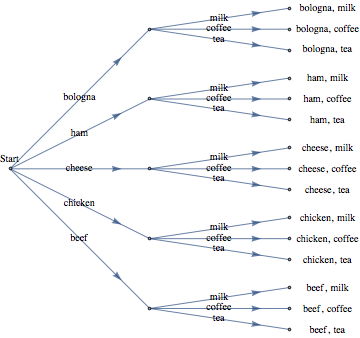
\includegraphics[width=\linewidth]{images/lunch.png}
\end{image}%
\tcblower
\end{figureptx}%
Every path that begins at the position labeled START and goes to the right can be interpreted as a choice of one of the five sandwiches followed by a choice of one of the three beverages. Note that considerable work is required to arrive at the number fifteen this way; but we also get more than just a number. The result is a complete list of all possible lunches. If we need to answer a question that starts with ``How many . . . ,'' enumeration would be done only as a last resort. In a later chapter we will examine more enumeration techniques.%
\par
An alternative method of solution for this example is to make the simple observation that there are five different choices for sandwiches and three different choices for beverages, so there are \(5 \cdot 3 = 15\) different lunches that can be ordered.%
\end{example}
\begin{example}{Counting elements in a cartesian product.}{x:example:cartesian-cardinality}%
Let \(A = \{a, b, c, d, e\}\) and \(B = \{1,2,3\}\). From Chapter 1 we know how to list the elements in \(A \times B = \{(a, 1), (a, 2), (a, 3), ..., (e, 3)\}\).  Since the first entry of each pair can be any one of the five elements \(a, b, c, d\), and \(e\), and since the second can be any one of the three numbers 1, 2, and 3, it is quite clear there are \(5 \cdot 3 = 15\) different elements in \(A \times B\).%
\end{example}
\begin{example}{A True-False Questionnaire.}{x:example:questionnaire}%
A person is to complete a true-false questionnaire consisting of ten questions. How many different ways are there to answer the questionnaire? Since each question can be answered in either of two ways (true or false), and there are ten questions, there are%
\begin{equation*}
2 \cdot 2 \cdot 2 \cdot 2 \cdot 2 \cdot 2 \cdot 2 \cdot 2 \cdot 2 \cdot 2 = 2^{10} = 1024
\end{equation*}
different ways of answering the questionnaire. The reader is encouraged to visualize the tree diagram of this example, but not to draw it!%
\end{example}
We formalize the procedures developed in the previous examples with the following rule and its extension.%
\end{subsectionptx}
%
%
\typeout{************************************************}
\typeout{Subsection 2.1.2 The Rule Of Products}
\typeout{************************************************}
%
\begin{subsectionptx}{The Rule Of Products}{}{The Rule Of Products}{}{}{x:subsection:rule-of-products}
\index{Rule Of Products, The}%
If two operations must be performed, and if the first operation can always be performed \(p_1\) different ways and the second operation can always be performed \(p_2\) different ways, then there are \(p_1 p_2\) different ways that the two operations can be performed.%
\par
Note: It is important that \(p_2\) does not depend on the option that is chosen in the first operation. Another way of saying this is that \(p_2\) is independent of the first operation. If \(p_2\) is dependent on the first operation, then the rule of products does not apply.%
\begin{example}{Reduced Lunch Possibilities.}{x:example:lunch-possibilites2}%
Assume in \hyperref[x:example:lunch-possibilies1]{Example~{\xreffont\ref{x:example:lunch-possibilies1}}}, coffee is not served with a beef or chicken sandwiches. Then by inspection of \hyperref[x:figure:lunch]{Figure~{\xreffont\ref{x:figure:lunch}}} we see that there are only thirteen different choices for lunch. The rule of products does not apply, since the choice of beverage depends on one's choice of a sandwich.%
\end{example}
\emph{Extended Rule Of Products.} The rule of products can be extended to include sequences of more than two operations. If \(n\) operations must be performed, and the number of options for each operation is \(p_1\), \(p_2, \dots, p_n\) respectively, with each \(p_i\)  independent of previous choices, then the \(n\) operations can be performed \(p_1 \cdot p_2 \cdot \cdots \cdot p_n\) different ways.%
\begin{example}{A Multiple Choice Questionnaire.}{x:example:another_questionnaire}%
A questionnaire contains four questions that have two possible answers and three questions with five possible answers. Since the answer to each question is independent of the answers to the other questions, the extended rule of products applies and there are \(2 \cdot 2 \cdot 2 \cdot 2 \cdot 5 \cdot 5 \cdot 5 = 2^4 \cdot 5^3 = 2000 \) different ways to answer the questionnaire.%
\end{example}
In Chapter 1 we introduced the power set of a set \(A\), \(\mathcal{P}(A)\), which is the set of all subsets of \(A\). Can we predict how many elements are in \(\mathcal{P}(A)\) for a given finite set \(A\)? The answer is yes, and in fact if \(\lvert A \rvert  = n\), then \(\lvert \mathcal{P}(A) \rvert = 2^{n}\).  The ease with which we can prove this fact demonstrates the power and usefulness of the rule of products. Do not underestimate the usefulness of simple ideas.%
\begin{theorem}{Power Set Cardinality Theorem.}{}{x:theorem:power-set-cardinality-theorem}%
\index{Power Set Cardinality Theorem}%
If \(A\) is a finite set, then \(\lvert \mathcal{P}(A) \rvert = 2^{\lvert A \rvert }\).%
\end{theorem}
\begin{proof}{}{g:proof:idm40464901152}
Proof: Consider how we might determine any \(B \in \mathcal{P}(A)\), where \(\lvert A \rvert =n\). For each element \(x \in A\) there are two choices, either \(x \in B\) or \(x \notin B\).  Since there are \(n\)  elements of \(A\)  we have, by the rule of products,%
\begin{equation*}
\underset{n \textrm{ factors}}{\underline{2 \cdot 2 \cdot  \cdots \cdot 2}}=  2^n
\end{equation*}
different subsets of \(A\). Therefore, \(\mathcal{P}(A)= 2^{n}\).%
\end{proof}
\end{subsectionptx}
%
%
\typeout{************************************************}
\typeout{Exercises 2.1.3 Exercises}
\typeout{************************************************}
%
\begin{exercises-subsection}{Exercises}{}{Exercises}{}{}{x:exercises:EXERCISES-FOR-SECTION-2-1}
\begin{divisionexercise}{1}{}{}{g:exercise:idm40464896064}%
In horse racing, to bet the ``daily double'' is to select the winners of the first two races of the day. You win only if both selections are correct. In terms of the number of horses that are entered in the first two races, how many different daily double bets could be made?%
\end{divisionexercise}%
\begin{divisionexercise}{2}{}{}{x:exercise:exercise-shortcut}%
Professor Shortcut records his grades using only his students' first and last initials. What is the smallest class size that will definitely force Prof. S. to use a different system?%
\end{divisionexercise}%
\begin{divisionexercise}{3}{}{}{g:exercise:idm40464891136}%
A certain shirt comes in four sizes and six colors. One also has the choice of a dragon, an alligator, or no emblem on the pocket. How many different shirts could you order?%
\end{divisionexercise}%
\begin{divisionexercise}{4}{}{}{g:exercise:idm40464889504}%
A builder of modular homes would like to impress his potential customers with the variety of styles of his houses. For each house there are blueprints for three different living rooms, four different bedroom configurations, and two different garage styles. In addition, the outside can be finished in cedar shingles or brick. How many different houses can be designed from these plans?%
\end{divisionexercise}%
\begin{divisionexercise}{5}{}{}{g:exercise:idm40464888464}%
The Pi Mu Epsilon mathematics honorary society of Outstanding University wishes to have a picture taken of its six officers. There will be two rows of three people. How many different way can the six officers be arranged?%
\end{divisionexercise}%
\begin{divisionexercise}{6}{}{}{g:exercise:idm40464886864}%
An automobile dealer has several options available for each of three different packages of a particular model car: a choice of two styles of seats in three different colors, a choice of four different radios, and five different exteriors. How many choices of automobile does a customer have?%
\end{divisionexercise}%
\begin{divisionexercise}{7}{}{}{g:exercise:idm40464885824}%
A clothing manufacturer has put out a mix-and-match collection consisting of two blouses, two pairs of pants, a skirt, and a blazer. How many outfits can you make? Did you consider that the blazer is optional? How many outfits can you make if the manufacturer adds a sweater to the collection?%
\end{divisionexercise}%
\begin{divisionexercise}{8}{}{}{g:exercise:idm40464884144}%
As a freshman, suppose you had to take two of four lab science courses, one of two literature courses, two of three math courses, and one of seven physical education courses. Disregarding possible time conflicts, how many different schedules do you have to choose from?%
\end{divisionexercise}%
\begin{divisionexercise}{9}{}{}{g:exercise:idm40464883136}%
(a) Suppose each single character stored in a computer uses eight bits. Then each character is represented by a different sequence of eight 0's and 1's called a bit pattern. How many different bit patterns are there? (That is, how many different characters could be represented?)%
\par
(b) How many bit patterns are palindromes (the same backwards as forwards)?%
\par
(c) How many different bit patterns have an even number of 1's?%
\end{divisionexercise}%
\begin{divisionexercise}{10}{}{}{g:exercise:idm40464877984}%
Automobile license plates in Massachusetts usually consist of three digits followed by three letters. The first digit is never zero. How many different plates of this type could be made?%
\end{divisionexercise}%
\begin{divisionexercise}{11}{}{}{g:exercise:idm40464877056}%
(a) Let \(A = \{1, 2, 3, 4\}\). Determine the number of different subsets of \(A\).%
\par
(b) Let \(A = \{1, 2, 3, 4, 5\}\). Determine the number of proper subsets of \(A\) .%
\end{divisionexercise}%
\begin{divisionexercise}{12}{}{}{g:exercise:idm40464872320}%
How many integers from 100 to 999 can be written in base ten without using the digit 7?%
\end{divisionexercise}%
\begin{divisionexercise}{13}{}{}{g:exercise:idm40464871584}%
Consider three persons, A, B, and C, who are to be seated in a row of three chairs. Suppose A and B are identical twins. How many seating arrangements of these persons can there be%
\par
%
\begin{multicols}{2}
\begin{enumerate}[label=(\alph*)]
\item{}If you are a total stranger?%
\item{}If you are A and B's mother?%
\end{enumerate}
\end{multicols}
%
\par
This problem is designed to show you that different people can have different correct answers to the same problem.%
\end{divisionexercise}%
\begin{divisionexercise}{14}{}{}{g:exercise:idm40464866944}%
How many ways can a student do a ten-question true-false exam if he or she can choose not to answer any number of questions?%
\end{divisionexercise}%
\begin{divisionexercise}{15}{}{}{g:exercise:idm40464866080}%
Suppose you have a choice of fish, lamb, or beef for a main course, a choice of peas or carrots for a vegetable, and a choice of pie, cake, or ice cream for dessert. If you must order one item from each category, how many different dinners are possible?%
\end{divisionexercise}%
\begin{divisionexercise}{16}{}{}{g:exercise:idm40464864576}%
Suppose you have a choice of vanilla, chocolate, or strawberry for ice cream, a choice of peanuts or walnuts for chopped nuts, and a choice of hot fudge or marshmallow for topping. If you must order one item from each category, how many different sundaes are possible?%
\end{divisionexercise}%
\begin{divisionexercise}{17}{}{}{g:exercise:idm40464863568}%
A questionnaire contains six questions each having yes-no answers. For each yes response, there is a follow-up question with four possible responses.%
\par
%
\begin{enumerate}[label=(\alph*)]
\item{}Draw a tree diagram that illustrates how many ways a single question in the questionnaire can be answered.%
\item{}How many ways can the questionnaire be answered?%
\end{enumerate}
%
\end{divisionexercise}%
\begin{divisionexercise}{18}{}{}{g:exercise:idm40464858288}%
Ten people are invited to a dinner party. How many ways are there of seating them at a round table? If the ten people consist of five men and five women, how many ways are there of seating them if each man must be surrounded by two women around the table?%
\end{divisionexercise}%
\begin{divisionexercise}{19}{}{}{g:exercise:idm40464856384}%
How many ways can you separate a set with \(n\)  elements into two nonempty subsets if the order of the subsets is immaterial? What if the order of the subsets is important?%
\end{divisionexercise}%
\begin{divisionexercise}{20}{}{}{g:exercise:idm40464854240}%
A gardener has three flowering shrubs and four nonflowering shrubs, where all shrubs are distinguishable from one another. He must plant these shrubs in a row using an alternating pattern, that is, a shrub must be of a different type from that on either side. How many ways can he plant these shrubs? If he has to plant these shrubs in a circle using the same pattern, how many ways can he plant this circle? Note that one nonflowering shrub will be left out at the end.%
\end{divisionexercise}%
\end{exercises-subsection}
\end{sectionptx}
%
%
\typeout{************************************************}
\typeout{Section 2.2 Permutations}
\typeout{************************************************}
%
\begin{sectionptx}{Permutations}{}{Permutations}{}{}{x:section:s-permutations}
%
%
\typeout{************************************************}
\typeout{Subsection 2.2.1 Ordering Things}
\typeout{************************************************}
%
\begin{subsectionptx}{Ordering Things}{}{Ordering Things}{}{}{g:subsection:idm40464852640}
A number of applications of the rule of products are of a specific type, and because of their frequent appearance they are given their own designation, permutations. Consider the following examples.%
\begin{example}{Ordering the elements of a set.}{x:example:ordering_a_set}%
How many different ways can we order the three different elements of the set \(A = \{a, b, c\}\)? Since we have three choices for position one, two choices for position two, and one choice for the third position, we have, by the rule of products, \(3 \cdot 2 \cdot 1 = 6\) different ways of ordering the three letters. We illustrate through a tree diagram.%
\begin{figureptx}{A tree to enumerate permutations of a three element set.}{x:figure:tree-of-permutations}{}%
\begin{image}{0.065}{0.87}{0.065}%
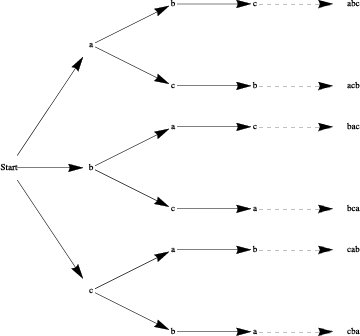
\includegraphics[width=\linewidth]{images/tree-of-permutations.png}
\end{image}%
\tcblower
\end{figureptx}%
Each of the six orderings is called a permutation of the set \(A\).%
\end{example}
\begin{example}{Ordering a schedule.}{x:example:ordering_a_schedule}%
A student is taking five courses in the fall semester. How many different ways can the five courses be listed? There are \(5 \cdot 4 \cdot 3 \cdot 2 \cdot 1 = 120\) different permutations of the set of courses.%
\end{example}
In each of the above examples of the rule of products we observe that:%
\par
%
\begin{enumerate}[label=(\alph*)]
\item{}We are asked to order or arrange elements from a single set.%
\item{}Each element is listed exactly once in each list (permutation). So if there are \(n\) choices for position one in a list, there are \(n - 1\) choices for position two, \(n - 2\) choices for position three, etc.%
\end{enumerate}
%
\begin{example}{Some orderings of a baseball team.}{x:example:some_orderings_of_a_baseball_team}%
The alphabetical ordering of the players of a baseball team is one permutation of the set of players. Other orderings of the players' names might be done by batting average, age, or height. The information that determines the ordering is called the key. We would expect that each key would give a different permutation of the names. If there are twenty-five players on the team, there are \(25 \cdot 24 \cdot 23 \cdot \cdots  \cdot 3 \cdot 2 \cdot 1\) different permutations of the players.%
\par
This number of permutations is huge. In fact it is 15511210043330985984000000, but writing it like this isn't all that instructive, while leaving it as a product as we originally had makes it easier to see where the number comes from.  We just need to find a more compact way of writing these products.%
\end{example}
We now develop notation that will be useful for permutation problems.%
\begin{definition}{Factorial.}{x:definition:Definition-Factorial}%
\index{Factorial}%
\label{g:notation:idm40464839344}%
If \(n\) is a positive integer then \(n\) factorial is the product of the first \(n\) positive integers and is denoted \(n!\). Additionally, we define zero factorial, \(0!\), to be 1.%
\end{definition}
The first few factorials are%
\begin{equation*}
\begin{array}{ccccccccc}
n & 0 & 1 & 2 & 3 & 4 & 5 & 6 &
7 \\
n! & 1 & 1 & 2 & 6 & 24 & 120 &
720 & 5040 \\
\end{array}\text{.}
\end{equation*}
%
\par
Note that \(4!\) is 4 times \(3!\), or 24, and \(5!\) is 5 times \(4!\), or 120. In addition, note that as \(n\) grows in size, \(n!\) grows extremely quickly. For example, \(11! = 39916800\). If the answer to a problem happens to be \(25!\), as in the previous example, you would never be expected to write that number out completely. However, a problem with an answer of \(\frac{25!}{23!}\) can be reduced to \(25 \cdot 24\), or 600.%
\par
If \(\lvert A \rvert = n \), there are \(n!\) ways of permuting all \(n\)  elements of \(A\) . We next consider the more general situation where we would like to permute \(k\) elements  out of a set of \(n\)  objects, where \(k \leq n\).%
\begin{example}{Choosing Club Officers.}{x:example:choosing-club-officers}%
A club of twenty-five members will hold an election for president, secretary, and treasurer in that order. Assume a person can hold only one position. How many ways are there of choosing these three officers? By the rule of products there are \(25 \cdot 24 \cdot 23\) ways of making a selection.%
\end{example}
\begin{definition}{Permutation.}{x:definition:permutation}%
\index{Permutation}%
An ordered arrangement of \(k\) elements selected from a set of \(n\) elements, \(0 \leq k \leq  n\), where no two elements of the arrangement are the same, is called a permutation of \(n\) objects taken \(k\) at a time. The total number of such permutations is denoted by \(P(n, k)\).%
\end{definition}
\begin{theorem}{Permutation Counting Formula.}{}{x:theorem:permutations-counting-formula}%
\index{Permutation Counting Formula}%
The number of possible permutations of \(k\)  elements taken from a set of \(n\)  elements is%
\begin{equation*}
P(n,k)=n \cdot (n-1) \cdot (n-2) \cdot  \cdots  \cdot (n-k+1) = \prod_{j=0}^{k-1} (n-j) = \frac{n!}{(n-k)!} \text{.}
\end{equation*}
%
\end{theorem}
\begin{proof}{}{g:proof:idm40464817728}
Case I: If \(k = n\) we have \(P(n,n)=n!=\frac{n!}{(n-n)!}\).%
\par
Case II: If \(0 \leq  k < n\),then we have \(k\)  positions to fill using \(n\) elements and%
\par
%
\begin{enumerate}[label=(\alph*)]
\item{}Position 1 can be filled by any one of \(n-0=n\)  elements%
\item{}Position 2 can be filled by any one of \(n-1\)  elements%
\item{}\(\displaystyle \cdots \)%
\item{}Position k can be filled by any one of \(n-(k-1)=n-k+1\)  elements%
\end{enumerate}
%
\par
Hence, by the rule of products,%
\begin{equation*}
P(n,k) = n \cdot(n - 1) \cdot (n - 2) \cdot \cdots \cdot (n - k + 1) = \frac{n!}{(n-k)!}\text{.}\qedhere
\end{equation*}
%
\end{proof}
It is important to note that the derivation of the permutation formula given above was done solely through the rule of products. This serves to reiterate our introductory remarks in this section that permutation problems are really rule-of-products problems.  We close this section with several examples.%
\begin{example}{Another example of choosing officers.}{x:example:more_club_officers}%
A club has eight members eligible to serve as president, vice-president, and treasurer. How many ways are there of choosing these officers?%
\par
Solution 1: Using the rule of products. There are eight possible choices for the presidency, seven for the vice-presidency, and six for the office of treasurer. By the rule of products there are \(8 \cdot 7\cdot 6 = 336\) ways of choosing these officers.%
\par
Solution 2: Using the permutation formula. We want the total number of permutations of eight objects taken three at a time:%
\begin{equation*}
P(8,3)=\frac{8!}{(8-3)!}=8 \cdot 7 \cdot 6 = 336
\end{equation*}
%
\end{example}
\begin{example}{Course ordering, revisited.}{x:example:course-ordering-revisited}%
To count the number of ways to order five courses, we can use the permutation formula. We want the number of permutations of five courses taken five at a time:%
\begin{equation*}
P(5,5)= \frac{5!}{(5-5)!}= 5!= 120\text{.}
\end{equation*}
%
\end{example}
\begin{example}{Ordering of digits under different conditions.}{x:example:ordering-digits}%
Consider only the digits 1, 2, 3, 4, and 5.%
\par
%
\begin{enumerate}[label=\alph*]
\item{}How many three-digit numbers can be formed if no repetition of digits can occur?%
\item{}How many three-digit numbers can be formed if repetition of digits is allowed?%
\item{}How many three-digit numbers can be formed if only non-consecutive repetition of digits are allowed?%
\end{enumerate}
%
\par
Solutions to (a): Solution 1: Using the rule of products. We have any one of five choices for digit one, any one of four choices for digit two, and three choices for digit three. Hence, \(5 \cdot 4 \cdot 3 = 60\) different three-digit numbers can be formed.%
\par
Solution 2; Using the permutation formula. We want the total number of permutations of five digits taken three at a time:%
\begin{equation*}
P(5,3)=\frac{5!}{(5-3)!}=5 \cdot 4 \cdot 3 = 60\text{.}
\end{equation*}
%
\par
Solution to (b): The definition of permutation indicates ``...no two elements in each list are the same.'' Hence the permutation formula cannot be used. However, the rule of products still applies. We have any one of five choices for the first digit, five choices for the second, and five for the third. So there are \(5 \cdot 5\cdot 5 = 125\) possible different three-digit numbers if repetition is allowed.%
\par
Solution to (c): Again, the rule of products applies here. We have any one of five choices for the first digit, but then for the next two digits we have four choices since we are not allowed to repeat the previous digit  So there are \(5 \cdot 4\cdot 4 = 80\) possible different three-digit numbers if only non-consecutive repetitions are allowed.%
\end{example}
\end{subsectionptx}
%
%
\typeout{************************************************}
\typeout{Exercises 2.2.2 Exercises}
\typeout{************************************************}
%
\begin{exercises-subsection}{Exercises}{}{Exercises}{}{}{g:exercises:idm40464852512}
\begin{divisionexercise}{1}{}{}{g:exercise:idm40464798064}%
If a raffle has three different prizes and there are 1,000 raffle tickets sold, how many different ways can the prizes be distributed?%
\end{divisionexercise}%
\begin{divisionexercise}{2}{}{}{g:exercise:idm40464796640}%
%
\begin{enumerate}[label=(\alph*)]
\item{}How many three-digit numbers can be formed from the digits 1, 2, 3 if no repetition of digits is allowed? List the three-digit numbers.%
\item{}How many two-digit numbers can be formed if no repetition of digits is allowed? List them.%
\item{}How many two-digit numbers can be obtained if repetition is allowed?%
\end{enumerate}
%
\end{divisionexercise}%
\begin{divisionexercise}{3}{}{}{g:exercise:idm40464794480}%
How many eight-letter words can be formed from the 26 letters in the alphabet? Even without concerning ourselves about whether the words make sense, there are two interpretations of this problem. Answer both.%
\end{divisionexercise}%
\begin{divisionexercise}{4}{}{}{g:exercise:idm40464792064}%
Let \(A\) be a set with \(\lvert A \rvert = n \). Determine%
\par
%
\begin{enumerate}[label=(\alph*)]
\item{}\(\lvert A^3 \rvert \)%
\item{}\(\lvert \{ (a, b, c) \mid a, b, c \in A \textrm{ and each coordinate is different}\} \rvert \)%
\end{enumerate}
%
\end{divisionexercise}%
\begin{divisionexercise}{5}{}{}{g:exercise:idm40464789024}%
The state finals of a high school track meet involves fifteen schools. How many ways can these schools be listed in the program?%
\end{divisionexercise}%
\begin{divisionexercise}{6}{}{}{g:exercise:idm40464787136}%
Consider the three-digit numbers that can be formed from the digits 1, 2, 3, 4, and 5 with no repetition of digits allowed.%
\par
a. How many of these are even numbers?%
\par
b. How many are greater than 250?%
\end{divisionexercise}%
\begin{divisionexercise}{7}{}{}{g:exercise:idm40464785760}%
All 15 players on the Tall U. basketball team are capable of playing any position.%
\begin{enumerate}[label=(\alph*)]
\item{}How many ways can the coach at Tall U. fill the five starting positions in a game?%
\item{}What is the answer if the center must be one of two players?%
\end{enumerate}
%
\end{divisionexercise}%
\begin{divisionexercise}{8}{}{}{g:exercise:idm40464782560}%
%
\begin{enumerate}[label=(\alph*)]
\item{}How many ways can a gardener plant five different species of shrubs in a circle?%
\item{}What is the answer if two of the shrubs are the same?%
\item{}What is the answer if all the shrubs are identical?%
\end{enumerate}
%
\end{divisionexercise}%
\begin{divisionexercise}{9}{}{}{g:exercise:idm40464779312}%
The president of the Math and Computer Club would like to arrange a meeting with six attendees, the president included. There will be three computer science majors and three math majors at the meeting. How many ways can the six people be seated at a circular table if the president does not want people with the same majors to sit next to one other?%
\end{divisionexercise}%
\begin{divisionexercise}{10}{}{}{g:exercise:idm40464777680}%
Six people apply for three identical jobs and all are qualified for the positions. Two will work in New York and the other one will work in San Diego. How many ways can the positions be filled?%
\end{divisionexercise}%
\begin{divisionexercise}{11}{}{}{g:exercise:idm40464776736}%
Let \(A = \{1, 2, 3, 4\} \). Determine the cardinality of%
\par
%
\begin{enumerate}[label=(\alph*)]
\item{}\(\{ (a_1,a_2) \mid a_1 \neq a_2 \}\)%
\item{}What is the answer to the previous part if \(\lvert A \rvert = n\)%
\item{}If \(\lvert A \rvert =n\), determine the number of \(m\)-tuples in \(A\), \(m \leq n\), where each coordinate is different from the other coordinates.%
\end{enumerate}
%
\end{divisionexercise}%
\end{exercises-subsection}
\end{sectionptx}
%
%
\typeout{************************************************}
\typeout{Section 2.3 Partitions of Sets and the Law of Addition}
\typeout{************************************************}
%
\begin{sectionptx}{Partitions of Sets and the Law of Addition}{}{Partitions of Sets and the Law of Addition}{}{}{x:section:s-partitions-and-law-of-addition}
%
%
\typeout{************************************************}
\typeout{Subsection 2.3.1 Partitions}
\typeout{************************************************}
%
\begin{subsectionptx}{Partitions}{}{Partitions}{}{}{g:subsection:idm40464767584}
One way of counting the number of students in your class would be to count the number in each row and to add these totals. Of course this problem is simple because there are no duplications, no person is sitting in two different rows. The basic counting technique that you used involves an extremely important first step, namely that of partitioning a set. The concept of a partition must be clearly understood before we proceed further.%
\begin{definition}{Partition.}{x:definition:partition}%
\index{Partition}%
A partition of set \(A\) is a set of one or more nonempty subsets of \(A\): \(A_1, A_2, A_3, \cdots\), such that every element of \(A\) is in exactly one set.  Symbolically,%
\par
%
\begin{enumerate}[label=(\alph*)]
\item{}\(A_1 \cup A_2 \cup A_3 \cup \cdots = A\)%
\item{}If  \(i \neq j\) then \(A_i \cap A_j = \emptyset\)%
\end{enumerate}
%
\end{definition}
The subsets in a partition are often referred to as blocks. Note how our definition allows us to partition infinite sets, and to partition a set into an infinite number of subsets. Of course, if \(A\)  is finite the number of subsets can be no larger than \(\lvert A \rvert \).%
\begin{example}{Some partitions of a four element set.}{x:example:some-partitions-4}%
Let \(A = \{a, b, c, d\}\). Examples of partitions of \(A\)  are:%
\par
%
\begin{itemize}[label=\textbullet]
\item{}\(\{\{a\}, \{b\}, \{c, d\}\}\)%
\item{}\(\{\{a, b\}, \{c, d\}\}\)%
\item{}\(\{\{a\}, \{b\}, \{c\}, \{d\}\}\)%
\end{itemize}
%
\par
How many others are there, do you suppose?%
\par
There are 15 different partitions.  The most efficient way to count them all is to classify them by the size of blocks.   For example, the partition \(\{\{a\}, \{b\}, \{c, d\}\}\) has block sizes 1, 1, and 2.%
\end{example}
\begin{example}{Some Integer Partitions.}{x:example:some-integer-partitions}%
Two examples of partitions of set of integers \(\mathbb{Z}\) are%
\par
%
\begin{itemize}[label=\textbullet]
\item{}\(\{\{n\} \mid n \in \mathbb{Z}\}\) and%
\item{}\(\{\{ n \in \mathbb{Z} \mid n < 0\}, \{0\},\{ n \in \mathbb{Z} \mid 0 < n \}\}\).%
\end{itemize}
%
\par
The set of subsets \(\{\{n \in \mathbb{Z} \mid n \geq 0\},\{n \in \mathbb{Z} \mid  n \leq 0\}\}\) is not a partition because the two subsets have a nonempty intersection. A second example of a non-partition is \(\{\{n \in \mathbb{Z} \mid  \lvert n \rvert = k\} \mid k = -1, 0, 1, 2, \cdots\}\) because one of the blocks, when \(k=-1\) is empty.%
\end{example}
One could also think of the concept of partitioning a set as a ``packaging problem.'' How can one ``package'' a carton of, say, twenty-four cans? We could use: four six-packs, three eight-packs, two twelve-packs, etc. In all cases: (a) the sum of all cans in all packs must be twenty-four, and (b) a can must be in one and only one pack.%
\end{subsectionptx}
%
%
\typeout{************************************************}
\typeout{Subsection 2.3.2 Addition Laws}
\typeout{************************************************}
%
\begin{subsectionptx}{Addition Laws}{}{Addition Laws}{}{}{g:subsection:idm40464747584}
\begin{theorem}{The Basic Law Of Addition:.}{}{x:theorem:basic-law-addition}%
\index{Basic Law Of Addition:}%
If \(A\) is a finite set, and if \(\{A_1,A_2,\ldots ,A_n\}\) is a partition of \(A\) , then%
\begin{equation*}
\lvert A \rvert = \lvert A_1 \rvert + \lvert A_2 \rvert + \cdots + \lvert A_n \rvert = \sum_{k=1}^n  \lvert A_k \rvert
\end{equation*}
%
\end{theorem}
The basic law of addition can be rephrased as follows: If \(A\)  is a finite set where \(A_1 \cup A_2 \cup \cdots \cup A_n = A\) and where \(A_i \cap A_j = \emptyset\) whenever \(i \neq j\), then%
\begin{equation*}
\lvert A \rvert = \lvert A_1 \cup A_2 \cup  \cdots \cup A_n  \rvert = \lvert A_1 \rvert + \lvert A_2 \rvert + \cdots + \lvert A_n \rvert 
\end{equation*}
%
\begin{example}{Counting All Students.}{x:example:counting-all-students}%
The number of students in a class could be determined by adding the numbers of students who are freshmen, sophomores, juniors, and seniors, and those who belong to none of these categories. However, you probably couldn't add the students by major, since some students may have double majors.%
\end{example}
\begin{example}{Counting Students in Disjoint Classes.}{x:example:student-counting-disjoint}%
The sophomore computer science majors were told they must take one and only one of the following courses that are open only to them: Cryptography, Data Structures, or Javascript. The numbers in each course, respectively, for sophomore CS majors, were 75, 60, 55. How many sophomore CS majors are there? The Law of Addition applies here. There are exactly \(75 + 60 + 55 = 190\) CS majors since the rosters of the three courses listed above would be a partition of the CS majors.%
\end{example}
\begin{example}{Counting Students in Non-disjoint Classes.}{x:example:student-counting-nondisjoint}%
It was determined that all junior computer science majors take at least one of the following courses: Algorithms, Logic Design, and Compiler Construction. Assume the number in each course was 75, 60 and 55, respectively for the three courses listed. Further investigation indicated ten juniors took all three courses, twenty-five took  Algorithms and Logic Design, twelve took Algorithms and Compiler Construction, and fifteen took Logic Design and Compiler Construction. How many junior C.S. majors are there?%
\par
\hyperref[x:example:student-counting-disjoint]{Example~{\xreffont\ref{x:example:student-counting-disjoint}}} was a simple application of the law of addition, however in this example some students are taking two or more courses, so a simple application of the law of addition would lead to double or triple counting. We rephrase information in the language of sets to describe the situation more explicitly.%
\par
\(A\) = the set of all junior computer science majors%
\par
\(A_1\) = the set of all junior computer science majors who took Algorithms%
\par
\(A_2\) = the set of all junior computer science majors who took Logic Design%
\par
\(A_3\) = the set of all junior computer science majors who took Compiler Construction%
\par
Since all junior CS majors must take at least one of the courses, the number we want is:%
\begin{equation*}
\lvert A \rvert = \lvert A_1 \cup A_2 \cup A_3 \rvert = \lvert A_1 \rvert + \lvert A_2 \rvert + \lvert A_3 \rvert - \textrm{repeats}.
\end{equation*}
%
\par
A Venn diagram is helpful to visualize the problem. In this case the universal set \(U\)  can stand for 	all students in the university.%
\begin{figureptx}{Venn Diagram}{x:figure:venn_diagram_CS_Students}{}%
\begin{image}{0}{1}{0}%
\IfFileExists{images/sageplot-venn-CS_Students.pdf}%
{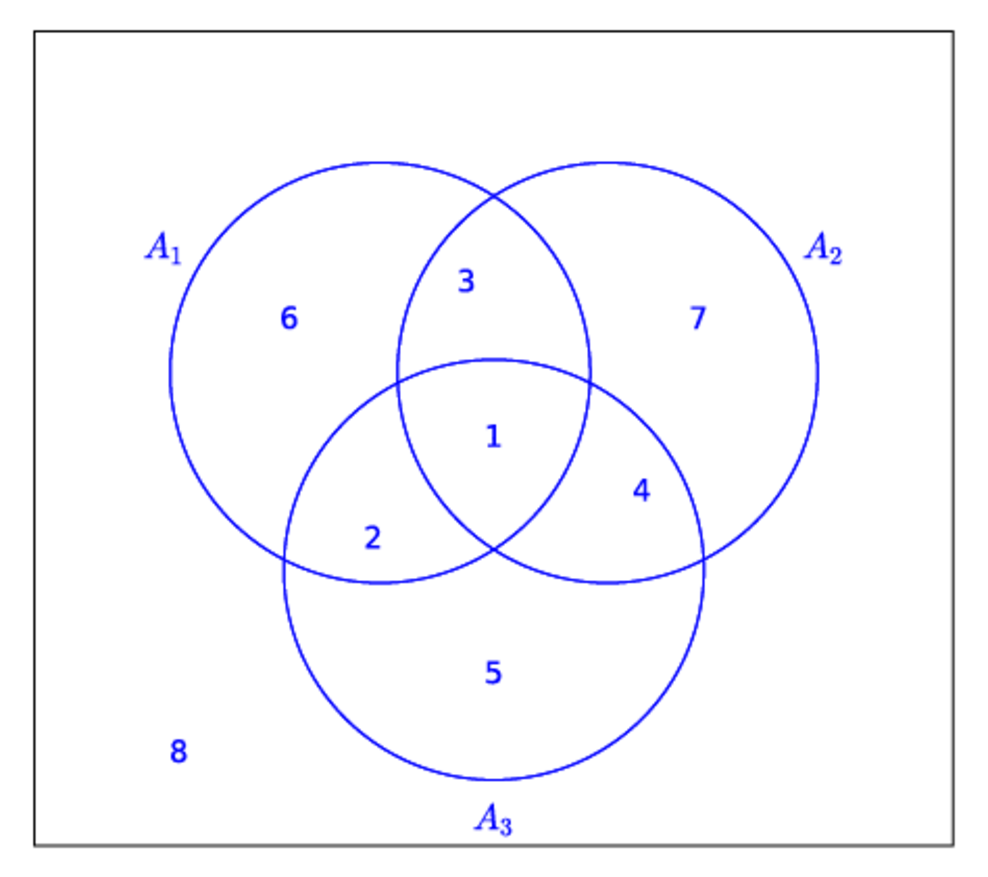
\includegraphics[width=\linewidth]{images/sageplot-venn-CS_Students.pdf}}%
{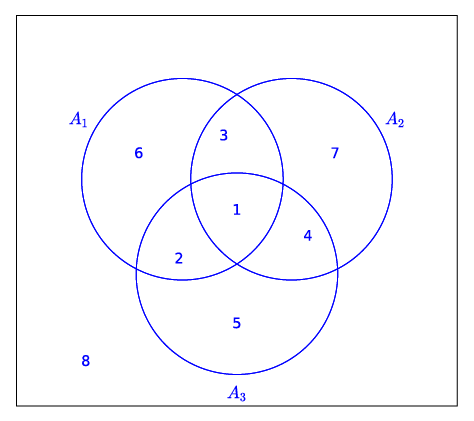
\includegraphics[width=\linewidth]{images/sageplot-venn-CS_Students.png}}
\end{image}%
\tcblower
\end{figureptx}%
We see that the whole universal set is naturally partitioned into subsets that are labeled by the numbers 1 through 8, and the set \(A\)  is  partitioned into subsets labeled 1 through 7. The region labeled 8 represents all students who are not junior CS majors.  Note also that students in the subsets labeled 2, 3, and 4 are double counted, and those in the subset labeled 1 are triple counted. To adjust, we must subtract the numbers in regions 2, 3 and 4.  This can be done by subtracting the numbers in the intersections of each pair of sets.  However, the individuals in region 1 will have been removed three times, just as they had been originally added three times.  Therefore, we must finally add their number back in.%
\par
%
\begin{equation*}
\begin{split}
\lvert A \rvert & =  \lvert A_1 \cup A_2 \cup A_3 \rvert \\ 
& = \lvert A_1 \rvert + \lvert A_2 \rvert + \lvert A_3 \rvert - \textrm{repeats} \\
& = \lvert A_1 \rvert + \lvert A_2 \rvert + \lvert A_3 \rvert - \textrm{duplicates} + \textrm{triplicates}  \\
& = \lvert A_1 \rvert + \lvert A_2 \rvert + \lvert A_3 \rvert - \left(\lvert A_1 \cap A_2 \rvert + \lvert A_1 \cap A_3 \rvert+ \lvert A_2 \cap A_3 \rvert \right) + \lvert A_1 \cap A_2 \cap A_3 \rvert  \\
& = 75 + 60 + 55 - 25 - 12 - 15 + 10 = 148 
\end{split}
\end{equation*}
%
\end{example}
The ideas used in this latest example gives rise to a basic counting technique:%
\begin{theorem}{Laws of Inclusion-Exclusion.}{}{x:theorem:inclusion-exclusion}%
\index{Inclusion-Exclusion, Laws of}%
Given finite sets \(A_1, A_2, A_3\), then%
\begin{enumerate}[label=(\alph*)]
\item\hypertarget{x:li:ie2}{}The Two Set Inclusion-Exclusion Law:%
\begin{equation*}
\lvert A_1 \cup A_2 \rvert =\lvert A_1 \rvert + \lvert A_2 \rvert - \lvert A_1 \cap A_2 \rvert  
\end{equation*}
%
\item\hypertarget{x:li:ie3}{}The Three Set Inclusion-Exclusion Law:%
\begin{equation*}
\begin{split}
\lvert A_1 \cup A_2 \cup A_3 \rvert & =\lvert A_1 \rvert + \lvert A_2 \rvert + \lvert A_3 \rvert\\
&\quad - (\lvert A_1 \cap A_2 \rvert + \lvert A_1 \cap A_3 \rvert+ \lvert A_2 \cap A_3 \rvert)\\
&\quad + \lvert A_1 \cap A_2 \cap A_3 \rvert
\end{split} 
\end{equation*}
%
\end{enumerate}
%
\end{theorem}
The inclusion-exclusion laws extend to more than three sets, as will be explored in the exercises.%
\par
In this section we saw that being able to partition a set into disjoint subsets gives rise to a handy counting technique. Given a set, there are many ways to partition depending on what one would wish to accomplish. One natural partitioning of sets is apparent when one draws a Venn diagram. This particular partitioning of a set will be discussed further in Chapters 4 and 13.%
\end{subsectionptx}
%
%
\typeout{************************************************}
\typeout{Exercises 2.3.3 Exercises}
\typeout{************************************************}
%
\begin{exercises-subsection}{Exercises}{}{Exercises}{}{}{x:exercises:exercises-2-3}
\begin{divisionexercise}{1}{}{}{g:exercise:idm40464719424}%
List all partitions of the set \(A =\{a, b, c\}\).%
\end{divisionexercise}%
\begin{divisionexercise}{2}{}{}{g:exercise:idm40464717792}%
Which of the following collections of subsets of the plane, \(\mathbb{R}^2\), are partitions?%
\par
%
\begin{enumerate}[label=(\alph*)]
\item{}\(\{ \{(x, y) \mid x + y = c \} \mid c \in \mathbb{R} \}\)%
\item{}The set of all circles in \(\mathbb{R}^2 \)%
\item{}The set of all circles in \(\mathbb{R}^2\) centered at the origin together with the set \(\{(0,0)\}\)%
\item{}\(\{\{(x, y)\} \mid (x, y) \in \mathbb{R}^2  \} \)%
\end{enumerate}
%
\end{divisionexercise}%
\begin{divisionexercise}{3}{}{}{g:exercise:idm40464712384}%
A student, on an exam paper, defined the term partition the following way: ``Let \(A\)  be a set. A partition of \(A\) is any set of nonempty subsets \(A_1, A_2, A_3, \dots\)  of \(A\) such that each element of \(A\) is in one of the subsets.''  Is this definition correct? Why?%
\end{divisionexercise}%
\begin{divisionexercise}{4}{}{}{g:exercise:idm40464708464}%
Let \(A_1\) and \(A_2\) be subsets of a set \(U\).   Draw a Venn diagram of this situation and shade in the subsets \(A_1 \cap A_2\), \(A_1^c \cap A_2\), \(A_1 \cap A_2^c\), and \(A_1^c \cap A_2^c\) . Use the resulting diagram and the definition of partition to convince yourself that the subset of these four subsets that are nonempty form a partition of \(U\).%
\end{divisionexercise}%
\begin{divisionexercise}{5}{}{}{g:exercise:idm40464707856}%
Show that \(\{\{2 n \mid n \in \mathbb{Z}\}, \{2 n + 1 \mid n \in \mathbb{Z}\}\}\) is a partition of \(\mathbb{Z}\). Describe this partition using only words.%
\end{divisionexercise}%
\begin{divisionexercise}{6}{}{}{g:exercise:idm40464701840}%
%
\begin{enumerate}[label=(\alph*)]
\item{}A group of 30 students were surveyed and it was found that 18 of them took Calculus and 12 took Physics. If all students took at least one course, how many took both Calculus and Physics? Illustrate using a Venn diagram.%
\item{}What is the answer to the question in part (a) if five students did not take either of the two courses? Illustrate using a Venn diagram.%
\end{enumerate}
%
\end{divisionexercise}%
\begin{divisionexercise}{7}{}{}{g:exercise:idm40464699200}%
A survey of 90 people, 47 of them played tennis and 42 of them swam. If 17 of them participated in both activities, how many of them participated in neither?%
\end{divisionexercise}%
\begin{divisionexercise}{8}{}{}{g:exercise:idm40464697520}%
A survey of 300 people found that 60 owned an iPhone, 75 owned a Blackberry, and 30 owned an Android phone. Furthermore, 40 owned both an iPhone and a Blackberry, 12 owned both an iPhone and an Android phone, and 8 owned a Blackberry and an Android phone. Finally, 3 owned all three phones.%
\par
%
\begin{enumerate}[label=(\alph*)]
\item{}How many people surveyed owned none of the three phones?%
\item{}How many people owned a Blackberry but not an iPhone?%
\item{}How many owned a Blackberry but not an Android?%
\end{enumerate}
%
\end{divisionexercise}%
\begin{divisionexercise}{9}{}{}{g:exercise:idm40464694736}%
Regarding the \hyperref[x:theorem:inclusion-exclusion]{Theorem~{\xreffont\ref{x:theorem:inclusion-exclusion}}},%
\begin{enumerate}[label=(\alph*)]
\item{}Use the two set inclusion-exclusion law  to derive the  three set inclusion-exclusion law. Note: A knowledge of basic set laws is needed for this exercise.%
\item{}State and derive the inclusion-exclusion law for four sets.%
\end{enumerate}
%
\end{divisionexercise}%
\begin{divisionexercise}{10}{}{}{g:exercise:idm40464687712}%
To complete your spring schedule, you must add Calculus and Physics. At 9:30, there are three Calculus sections and two Physics sections; while at 11:30, there are two Calculus sections and three Physics sections.  How many ways can you complete your schedule if your only open periods are 9:30 and 11:30?%
\end{divisionexercise}%
\begin{divisionexercise}{11}{}{}{g:exercise:idm40464686656}%
The definition of \(\mathbb{Q}  = \{a/b \mid a, b \in \mathbb{Z}, b \neq 0\}\) given in Chapter 1 is  awkward. If we use the definition to list elements in \(\mathbb{Q}\), we will have duplications such as \(\frac{1}{2}\), \(\frac{-2}{-4}\) and \(\frac{300}{600}\)   Try to write a more precise definition of the rational numbers so that there is no duplication of elements.%
\end{divisionexercise}%
\end{exercises-subsection}
\end{sectionptx}
%
%
\typeout{************************************************}
\typeout{Section 2.4 Combinations and the Binomial Theorem}
\typeout{************************************************}
%
\begin{sectionptx}{Combinations and the Binomial Theorem}{}{Combinations and the Binomial Theorem}{}{}{x:section:s-combinations-and-the-binomial-theorem}
%
%
\typeout{************************************************}
\typeout{Subsection 2.4.1 Combinations}
\typeout{************************************************}
%
\begin{subsectionptx}{Combinations}{}{Combinations}{}{}{x:subsection:combinations}
\index{Combinations}%
In Section 2.1 we investigated the most basic concept in combinatorics, namely, the rule of products. It is of paramount importance to keep this fundamental rule in mind. In Section 2.2 we saw a subclass of rule-of-products problems, permutations, and we derived a formula as a computational aid to assist us. In this section we will investigate another counting formula, one that is used to count combinations, which are subsets of a certain size.%
\par
In many rule-of-products applications the ordering is important, such as the batting order of a baseball team. In other cases it is not important, as in placing coins in a vending machine or in the listing of the elements of a set. Order is important in permutations. Order is not important in combinations.%
\begin{example}{Counting Permutations.}{x:example:counting-permuations-multiple-ways}%
How many different ways are there to permute three letters from the set \(A = \{a, b, c, d\}\)?  From the \hyperref[x:theorem:permutations-counting-formula]{Permutation Counting Formula} there are \(P(4,3)=\frac{4!}{(4-3)!} = 24\) different orderings of three letters from \(A\)%
\end{example}
\begin{example}{Counting with No Order.}{x:example:four-choose-three}%
How many ways can we select a set of three letters from  \(A = \{a, b, c, d\}\)?  Note here that we are not concerned with the order of the three letters. By trial and error, abc, abd, acd, and bcd are the only listings possible. To repeat, we were looking for all three-element subsets of the set \(A\). Order is not important in sets. The notation for choosing 3 elements from 4 is most commonly \(\binom{4}{3}\) or occasionally \(C(4,3)\), either of which is read ``4 choose 3'' or the number of combinations for four objects taken three at a time.%
\end{example}
\begin{definition}{Binomial Coefficient.}{x:definition:binomial-coefficient}%
\index{Binomial Coefficient}%
\label{g:notation:idm40464672528}%
Let \(n\) and \(k\) be nonnegative integers.  The binomial coefficient \(\binom{n}{k}\) represents the number of combinations of \(n\) objects taken \(k\) at a time, and is read ``\(n\) choose \(k\).''%
\end{definition}
We would now like to investigate the relationship between permutation and combination problems in order to derive a formula for \(\binom{n}{k}\)%
\par
Let us reconsider the \hyperref[x:example:four-choose-three]{Counting with No Order}. There are \(3 ! = 6\) different orderings for each of the three-element subsets. The table below lists each subset of \(A\)  and all permutations of each subset on the same line.%
\begin{equation*}
\begin{array}{cc}
\textrm{subset} & \textrm{permutations} \\
\{a, b, c\} & abc,acb,bca,bac,cab,cba \\
\{a, b, d\} & abd,adb,bda,bad,dab,dba \\
\{a, c, d\} & acd,adc,cda,cad,dac,dca \\
\{b, c, d\} & bcd,bdc,cdb,cbd,dbc,dcb \\
\end{array}\text{.}
\end{equation*}
%
\par
Hence, \(\binom{4}{3} = \frac{P(4,3)}{3!} = \frac{4!}{(4-3)! \cdot 3!} = 4\)%
\par
We generalize this result in the following theorem:%
\begin{theorem}{Binomial Coefficient Formula.}{}{x:theorem:binomial-coefficient-formula}%
\index{Binomial Coefficient Formula}%
If \(n\) and \(k\) are nonnegative integers with \(0 \leq k \leq n\), then the number \(k\)-element subsets of an \(n\) element set is equal to%
\begin{equation*}
\binom{n}{k} = \frac{n!}{(n-k)! \cdot k!} \text{.}
\end{equation*}
%
\end{theorem}
\begin{proof}{}{g:proof:idm40464660096}
Proof 1: There are \(k!\) ways of ordering the elements of any \(k\) element set. Therefore,%
\begin{equation*}
\binom{n}{k} = \frac{P(n,k)}{k!} = \frac{n!}{(n-k)! k!}.\text{.}
\end{equation*}
%
\par
Proof 2: To ``construct'' a permutation of \(k\)  objects from a set of \(n\) elements, we can first choose one of the subsets of objects and second, choose one of the \(k!\)  permutations of those objects. By the rule of products,%
\begin{equation*}
P(n,k) = \binom{n}{k} \cdot k!
\end{equation*}
and solving for \(\binom{n}{k}\) we get the desired formula.%
\end{proof}
\begin{example}{Flipping Coins.}{x:example:flipping-coins}%
Assume an evenly balanced coin is tossed five times. In how many ways can three heads be obtained? This is a combination problem, because the order in which the heads appear does not matter. We can think of this as a situation involving sets by considering the set of flips of the coin, 1 through 5, in which heads comes up.   The number of ways to get three heads is \(\binom{5}{3}= \frac{5 \cdot 4}{2 \cdot 1} = 10\).%
\end{example}
\begin{example}{Counting five ordered flips two ways.}{x:example:five-flips}%
We determine the total number of ordered ways a fair coin can land if tossed five consecutive times. The five tosses can produce any one of the following mutually exclusive, disjoint events: 5 heads, 4 heads, 3 heads, 2 heads, 1 head, or 0 heads.  For example, by the previous example, there are \(\binom{5}{3}=10\) sequences in which three heads appear. Counting the other possibilities in the same way, by the law of addition we have:%
\begin{equation*}
\binom{5}{5}+\binom{5}{4}+\binom{5}{3}+\binom{5}{2}+\binom{5}{1}+\binom{5}{0}= 1 + 5 +10+10+5+1 = 32
\end{equation*}
ways to observe the five flips.%
\par
Of course, we could also have applied the extended rule of products, and since there are two possible outcomes for each of the five tosses, we have \(2^5 = 32\) ways.%
\end{example}
You might think that counting something two ways is a waste of time but solving a problem two different ways often is instructive and leads to valuable insights. In this case, it suggests a general formula for the sum \(\sum_{k=0}^n \binom{n}{k}\). In the case of \(n = 5\), we get \(2^5\) so it is reasonable to expect that the general sum is \(2^n\), and it is.  A logical argument to prove the general statment simply involves generalizing the previous example to \(n\) coin flips.%
\begin{example}{A Committee of Five.}{x:example:committee-of-five}%
A committee usually starts as an unstructured set of people selected from a larger membership. Therefore, a committee can be thought of as a combination. If a club of 25 members has a five-member social committee, there are \(\binom{25}{5}=\frac{25\cdot 24\cdot 23\cdot 22\cdot 21}{5!} = 53130\) different possible social committees. If any structure or restriction is placed on the way the social committee is to be selected, the number of possible committees will probably change. For example, if the club has a rule that the treasurer must be on the social committee, then the number of possibilities is reduced to \(\binom{24}{4}=\frac{24\cdot 23\cdot 22\cdot 21}{4!} = 10626\).%
\par
If we further require that a chairperson other than the treasurer be selected for the social committee, we have  \(\binom{24}{4} \cdot 4 = 42504\) different possible social committees. The choice of the four non-treasurers accounts for the factor \(\binom{24}{4}\) while the need to choose a chairperson accounts for the 4.%
\end{example}
\begin{example}{Binomial Coefficients - Extreme Cases.}{x:example:extreme-binomial-cases}%
By simply applying the definition of a \hyperref[x:definition:binomial-coefficient]{Binomial Coefficient} as a number of subsets we see that there is \(\binom{n}{0} = 1\) way of choosing a combination of zero elements from a set of \(n\). In addition, we see that   there is \(\binom{n}{n} = 1\) way of choosing a combination of \(n\) elements from a set of \(n\).%
\par
We could compute these values using the formula we have developed, but no arithmetic is really needed here.  Other properties of binomial coefficients that can be derived using the subset definition will be seen in the exercises%
\end{example}
\end{subsectionptx}
%
%
\typeout{************************************************}
\typeout{Subsection 2.4.2 The Binomial Theorem}
\typeout{************************************************}
%
\begin{subsectionptx}{The Binomial Theorem}{}{The Binomial Theorem}{}{}{x:subsection:the-binomial-theorem}
The binomial theorem gives us a formula for expanding \(( x + y )^{n}\), where \(n\)  is a nonnegative integer. The coefficients of this expansion are precisely the binomial coefficients that we have used to count combinations. Using high school algebra we can  expand the expression for integers from 0 to 5:%
\par
%
\begin{equation*}
\begin{array}{cc}
n & (x + y)^n \\
0 & 1 \\
1 & x+y \\
2 & x^2+2 x y+y^2 \\
3 & x^3+3 x^2 y+3 x y^2+y^3 \\
4 & x^4+4 x^3 y+6 x^2 y^2+4 x y^3+y^4
\\
5 & x^5+5 x^4 y+10 x^3 y^2+10 x^2
y^3+5 x y^4+y^5 \\
\end{array}
\end{equation*}
%
\par
In the expansion of \((x + y)^{5} \)  we note that the coefficient of the third term is \(\binom{5}{3} = 10\), and that of the sixth term is  \(\binom{5}{5}=1\). We can rewrite the expansion as%
\begin{equation*}
\binom{5}{0} x^5+\binom{5}{1} x^4 y+\binom{5}{2} x^3 y^2+\binom{5}{3} x^2 y^3+\binom{5}{4} x y^4+ \binom{5}{5} y^5\text{.}
\end{equation*}
%
\par
In summary, in the expansion of \(( x + y )^{n}\) we note:%
\par
%
\begin{enumerate}[label=(\alph*)]
\item{}The first term is \(x^n\) and the last term is \(y^n\).%
\item{}With each successive term, exponents of \(x\) decrease by 1 as those of \(y\) increase by 1. For any term the sum of the exponents is \(n\).%
\item{}The coefficient of \(x^{n-k} y^k\) is \(\binom{n}{k}\).%
\item{}The triangular array of binomial coefficients is called Pascal's triangle after the seventeenth-century French mathematician Blaise Pascal. Note that each number in the triangle other than the 1's at the ends of each row is the sum of the two numbers to the right and left of it in the row above.%
\end{enumerate}
%
\begin{theorem}{The Binomial Theorem.}{}{x:theorem:binomial-theorem}%
\index{Binomial Theorem, The}%
If \(n \geq  0\), and \(x\) and \(y\) are numbers, then%
\begin{equation*}
(x+y)^{n} = \sum_{k=0}^n \binom{n}{k} x^{n-k} y^k\text{.}
\end{equation*}
%
\end{theorem}
\begin{proof}{}{g:proof:idm40464621536}
This theorem will be proven using a logical procedure called mathematical induction, which will be introduced in Chapter 3.%
\end{proof}
\begin{example}{Identifying a term in an expansion.}{x:example:term-in-an-expansion}%
Find the third term in the expansion of \((x-y)^{4} = (x+(-y))^{4}\). The third term,  when \(k=2\), is \(\binom{4}{2} x^{4-2} (-y)^2 = 6 x^2 y^2\).%
\end{example}
\begin{example}{A Binomial Expansion.}{x:example:a-full-expansion}%
Expand \((3 x - 2 )^{3}\).  If we replace \(x\)  and \(y\)  in the Binomial Theorem with \(3x\) and \(-2\), respectively, we get%
\begin{equation*}
\begin{split} 
\sum_{k=0}^3 \binom{3}{k} (3x)^{n-k} (-2)^k & = \binom{3}{0} (3x)^{3} (-2)^0 + \binom{3}{1} (3x)^{2} (-2)^1 + \binom{3}{2} (3x)^{1} (-2)^2 + \binom{3}{3} (3x)^{0} (-2)^3 \\
& = 27 x^3 - 54 x^2 + 36 x - 8 
\end{split}\text{.}
\end{equation*}
%
\end{example}
\end{subsectionptx}
%
%
\typeout{************************************************}
\typeout{Subsection 2.4.3 SageMath Note}
\typeout{************************************************}
%
\begin{subsectionptx}{SageMath Note}{}{SageMath Note}{}{}{x:subsection:sage-bridge-hands}
\index{SageMath Note!bridge hands}%
A bridge hand is a 13 element subset of a standard 52 card deck. The order in which the cards come to the player doesn't matter. From the point of view of a single player, the number of possible bridge hands is \(\binom{52}{13}\), which can be easily computed with \(Sage\).%
\begin{sageinput}
binomial(52,13)
\end{sageinput}
\begin{sageoutput}
635013559600
\end{sageoutput}
In bridge, the location of a hand in relation to the dealer has some bearing on the game. An even truer indication of the number of possible hands takes into account \(each\)  player's possible hand. It is customary  to refer to bridge positions as West, North, East and South. We can apply the rule of product to get the total number of bridge hands with the following logic. West can get any of the \(\binom{52}{13}\) hands identified above. Then North get 13 of the remaining 39 cards and so has  \(\binom{39}{13}\) possible hands. East then gets 13 of the 26 remaining cards, which has \(\binom{26}{13}\)  possibilities. South gets the remaining cards. Therefore the number of bridge hands is computed using the Product Rule.%
\begin{sageinput}
binomial(52,13)*binomial(39,13)*binomial(26,13)
\end{sageinput}
\begin{sageoutput}
53644737765488792839237440000
\end{sageoutput}
\end{subsectionptx}
%
%
\typeout{************************************************}
\typeout{Exercises 2.4.4 Exercises}
\typeout{************************************************}
%
\begin{exercises-subsection}{Exercises}{}{Exercises}{}{}{x:exercises:exercises-2-4}
\begin{divisionexercise}{1}{}{}{g:exercise:idm40464607440}%
The judiciary committee at a college is made up of three faculty members and four students. If ten faculty members and 25 students have been nominated for the committee, how many judiciary committees could be formed at this point?%
\end{divisionexercise}%
\begin{divisionexercise}{2}{}{}{g:exercise:idm40464605824}%
Suppose that a single character is stored in a computer using eight bits.%
\par
a. How many bit patterns have exactly three 1's?%
\par
b. How many bit patterns have at least two 1's?%
\par\smallskip%
\noindent\textbf{\blocktitlefont Hint}.\hypertarget{g:hint:idm40464604432}{}\quad{}Think of the set of positions that contain a 1 to turn this is into a question about sets.%
\end{divisionexercise}%
\begin{divisionexercise}{3}{}{}{g:exercise:idm40464602400}%
How many subsets of \(\{1, 2, 3, \dots , 10\}\) contain at least seven elements?%
\end{divisionexercise}%
\begin{divisionexercise}{4}{}{}{g:exercise:idm40464600432}%
The congressional committees on mathematics and computer science are made up of five representatives each, and a congressional rule is that the two committees must be disjoint. If there are 385 members of congress, how many ways could the committees be selected?%
\end{divisionexercise}%
\begin{divisionexercise}{5}{}{}{g:exercise:idm40464600080}%
\index{Lattice Paths}The image below shows a 6 by 6 grid and an example of a \terminology{lattice path} that could be taken from \((0,0)\)  to \((6,6)\), which is a path taken by traveling along grid lines going only to the right and up. How many different lattice paths are there of this type?  Generalize to the case of lattice paths from \((0,0)\) to \((m,n)\)  for any nonnegative integers \(m\) and \(n\).%
\begin{figureptx}{A lattice path}{x:figure:fig-lattice-path-6}{}%
\begin{image}{0.25}{0.5}{0.25}%
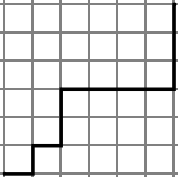
\includegraphics[width=\linewidth]{images/fig-lattice-path-6.png}
\end{image}%
\tcblower
\end{figureptx}%
\par\smallskip%
\noindent\textbf{\blocktitlefont Hint}.\hypertarget{g:hint:idm40464594032}{}\quad{}Think of each path as a sequence of instructions to go right (R) and up (U).%
\end{divisionexercise}%
\begin{divisionexercise}{6}{}{}{g:exercise:idm40464590528}%
How many of the lattice paths from \((0,0)\) to \((6,6)\) pass through \((3,3)\) as the one in \hyperref[x:figure:fig-lattice-path-6]{Figure~12} does?%
\end{divisionexercise}%
\begin{divisionexercise}{7}{}{}{g:exercise:idm40464587744}%
A poker game is played with 52 cards.  At the start of a game, each player gets five of the cards.  The order in which cards are dealt doesn't matter.%
\begin{enumerate}[label=(\alph*)]
\item{}How many ``hands'' of five cards are possible?%
\item{}If there are four people playing, how many initial five-card ``hands'' are possible, taking into account all players and their positions at the table?  Position with respect to the dealer does matter.%
\end{enumerate}
%
\end{divisionexercise}%
\begin{divisionexercise}{8}{}{}{g:exercise:idm40464582992}%
A flush in a five-card poker hand is five cards of the same suit. The suits are spades, clubs, diamonds and hearts.  How many spade flushes are possible in a 52-card deck? How many flushes are possible in any suit?%
\end{divisionexercise}%
\begin{divisionexercise}{9}{}{}{g:exercise:idm40464581440}%
How many five-card poker hands using 52 cards contain exactly two aces?%
\end{divisionexercise}%
\begin{divisionexercise}{10}{}{}{g:exercise:idm40464580192}%
In poker, a full house is three-of-a-kind and a pair in one hand; for example, three fives and two queens. How many full houses are possible from a 52-card deck?  You can use the sage cell in the \hyperref[x:subsection:sage-bridge-hands]{SageMath Note} to do this calculation, but also write your answer in terms of binomial coefficients.%
\end{divisionexercise}%
\begin{divisionexercise}{11}{}{}{g:exercise:idm40464578288}%
A class of twelve computer science students are to be divided into three groups of 3, 4, and 5 students to work on a project. How many ways can this be done if every student is to be in exactly one group?%
\end{divisionexercise}%
\begin{divisionexercise}{12}{}{}{g:exercise:idm40464576784}%
Explain in words why the following equalities are true based on number of subsets,  and then verify the equalities using the formula for binomial coefficients.%
\par
%
\begin{enumerate}[label=(\alph*)]
\item{}\(\binom{n}{1} = n\)%
\item{}\(\binom{n}{k} = \binom{n}{n-k}\), \(0 \leq k \leq n\)%
\end{enumerate}
%
\end{divisionexercise}%
\begin{divisionexercise}{13}{}{}{g:exercise:idm40464573408}%
There are ten points, \(P_1, P_2, \dots , P_{10}\) on a plane, no three on the same line.%
\par
%
\begin{enumerate}[label=(\alph*)]
\item{}How many lines are determined by the points?%
\item{}How many triangles are determined by the points?%
\end{enumerate}
%
\end{divisionexercise}%
\begin{divisionexercise}{14}{}{}{g:exercise:idm40464569264}%
How many ways can \(n\)  persons be grouped into pairs when \(n\)  is even? Assume the order of the pairs matters, but not the order within the pairs. For example, if \(n=4\), the six different groupings would be%
\begin{equation*}
\begin{array}{cc}
\{1,2\} & \{3,4\} \\
\{1,3\} & \{2,4\} \\
\{1,4\} & \{2,3\} \\
\{2,3\} & \{1,4\} \\
\{2,4\} & \{1,3\} \\
\{3,4\} & \{1,2\} \\
\end{array}
\end{equation*}
%
\end{divisionexercise}%
\begin{divisionexercise}{15}{}{}{g:exercise:idm40464566704}%
Use the binomial theorem to prove that if \(A\) is a finite set, then \(\lvert P(A)\rvert =2^{\lvert A  \rvert}\)%
\end{divisionexercise}%
\begin{divisionexercise}{16}{}{}{g:exercise:idm40464564944}%
%
\begin{enumerate}[label=(\alph*)]
\item{}A state's lottery involves choosing six different numbers out of a possible 36. How many ways can a person choose six numbers?%
\item{}What is the probability of a person winning with one bet?%
\end{enumerate}
%
\end{divisionexercise}%
\begin{divisionexercise}{17}{}{}{g:exercise:idm40464559840}%
Use the binomial theorem to calculate \(9998^3\).%
\par\smallskip%
\noindent\textbf{\blocktitlefont Hint}.\hypertarget{g:hint:idm40464558816}{}\quad{}\(9998 = 10000-2\)%
\end{divisionexercise}%
\begin{divisionexercise}{18}{}{}{g:exercise:idm40464557568}%
In the card game Blackjack, there are one or more players and a dealer.  Initially, each player is dealt two cards and the dealer is dealt one card down and one facing up.  As in bridge, the order of the hands, but not the order of the cards in the hands, matters.  Starting with a single 52 card deck, and three players, how many ways can the first two cards be dealt out?  You can use the sage cell in the \hyperref[x:subsection:sage-bridge-hands]{SageMath Note} to do this calculation.%
\end{divisionexercise}%
\end{exercises-subsection}
\end{sectionptx}
\end{chapterptx}
%
%
\typeout{************************************************}
\typeout{Chapter 3 Logic}
\typeout{************************************************}
%
\begin{chapterptx}{Logic}{}{Logic}{}{}{x:chapter:chapter3}
\begin{introduction}{}%
\begin{poem}%
\poemTitle{formal logic}
\begin{stanza}
\poemlineleft{You can write any letters you choose;}
\poemlineleft{\terminology{Formal logic}, though, likes \(p\)'s and \(q\)'s}
\poemlineleft{To form statements — a lot,}
\poemlineleft{Using IF, OR, AND, NOT —}
\poemlineleft{To determine the falses and trues.}
\end{stanza}
\poemauthorleft{Goldie, The Omnificent English Dictionary In Limerick Form}
\end{poem}
In this chapter, we will introduce some of the basic concepts of mathematical logic. In order to fully understand some of the later concepts in this 	book, you must be able to recognize valid logical arguments. Although these arguments will usually be applied to mathematics, they employ the same techniques that are used by a lawyer in a courtroom or a physician examining a patient. An added reason for the importance of this chapter is that the circuits that make up digital computers are designed using the same algebra of propositions that we will be discussing.%
\end{introduction}%
%
%
\typeout{************************************************}
\typeout{Section 3.1 Propositions and Logical Operators}
\typeout{************************************************}
%
\begin{sectionptx}{Propositions and Logical Operators}{}{Propositions and Logical Operators}{}{}{x:section:s-propositions-logic-operators}
%
%
\typeout{************************************************}
\typeout{Subsection 3.1.1 Propositions}
\typeout{************************************************}
%
\begin{subsectionptx}{Propositions}{}{Propositions}{}{}{x:subsection:ss-propositions}
\begin{definition}{Proposition.}{x:definition:def-proposition}%
\index{Proposition}%
A proposition is a sentence to which one and only one of the terms \emph{true} or \emph{false} can be meaningfully applied.%
\end{definition}
\begin{example}{Some Propositions.}{x:example:some-propositions}%
``Four is even,'', ``\(4 \in  \{1,3, 5\}\)'' and ``\(43 > 21\)'' are propositions.%
\end{example}
In traditional logic, a declarative statement with a definite truth value is considered a proposition. Although our ultimate aim is to discuss mathematical logic, we won't separate ourselves completely from the traditional setting. This is natural because the basic assumptions, or postulates, of mathematical logic are modeled after the logic we use in everyday life. Since compound sentences are frequently used in everyday speech, we expect that logical propositions contain connectives like the word ``and.'' The statement ``Europa supports life or Mars supports life'' is a proposition and, hence, must have a definite truth value. Whatever that truth value is, it should be the same as the truth value of ``Mars supports life or Europa supports life.''%
\end{subsectionptx}
%
%
\typeout{************************************************}
\typeout{Subsection 3.1.2 Logical Operations}
\typeout{************************************************}
%
\begin{subsectionptx}{Logical Operations}{}{Logical Operations}{}{}{x:subsection:ss-logical-operations}
There are several ways in which we commonly combine simple statements into compound ones. The words\slash{}phrases \emph{and}, \emph{or}, \emph{not}, \emph{if ... then...}, and \emph{...if and only if ...} can be added to one or more propositions to create a new proposition. To avoid any confusion, we will precisely define each one's meaning and introduce its standard symbol.  With the exception of negation (\emph{not}), all of the operations act on pairs of propositions. Since each proposition has two possible truth values, there are four ways that truth can be assigned to two propositions. In defining the effect that a logical operation has on two propositions, the result must be specified for all four cases. The most convenient way of doing this is with a truth table, which we will illustrate by defining the word \emph{and}.%
\begin{definition}{Logical Conjunction.}{x:definition:def-conjunction}%
\index{Conjunction, Logical}%
\label{g:notation:idm40464534048}%
If \(p\) and \(q\) are propositions, their conjunction, \(p \textrm{ and } q\) (denoted \(p \land q\)), is defined by the truth table%
\begin{equation*}
\begin{array}{ccc}
p & q & p\land q \\
\hline
0 & 0 & 0 \\
0 & 1 & 0 \\
1 & 0 & 0 \\
1 & 1 & 1 \\
\end{array}
\end{equation*}
%
\end{definition}
Notes:%
\par
%
\begin{enumerate}[label=(\alph*)]
\item{}To read this truth table, you must realize that any one line represents a case: one possible set of values for \(p\) and \(q\).%
\item{}The numbers 0 and 1 are used to denote false and true, respectively. This is consistent with the way that many programming languages treat logical, or Boolean, variables since a single bit, 0 or 1, can represent a truth value.%
\item{}For each case, the symbol under \(p\) represents the truth value of \(p\). The same is true for \(q\). The symbol under \(p \land q\) represents its truth value for that case. For example, the second row of the truth table represents the case in which \(p\) is false, \(q\) is true, and the resulting truth value for \(p \land q\) is false. As in everyday speech, \(p \land q\) is true only when both propositions are true.%
\item{}Just as the letters \(x\), \(y\) and \(z\) are frequently used in algebra to represent numeric variables, \(p\), \(q\) and \(r\) seem to be the most commonly used symbols for logical variables. When we say that \(p\) is a logical variable, we mean that any proposition can take the place of \(p\).%
\item{}One final comment: The order in which we list the cases in a truth table is standardized in this book. If the truth table involves two simple propositions, the numbers under the simple propositions can be interpreted as the two-digit binary integers in increasing order, 00, 01, 10, and 11, for 0, 1, 2, and 3, respectively.%
\end{enumerate}
%
\begin{definition}{Logical Disjunction.}{x:definition:def-disjunction}%
\index{Disjunction, Logical}%
\label{g:notation:idm40464517168}%
If \(p\) and \(q\) are propositions, their disjunction, \(p \textrm{ or } q\) (denoted \(p \lor q\)), is defined by the truth table%
\begin{equation*}
\begin{array}{ccc}
p & q & p\lor q \\
\hline
0 & 0 & 0 \\
0 & 1 & 1 \\
1 & 0 & 1 \\
1 & 1 & 1 \\
\end{array}
\end{equation*}
%
\end{definition}
\begin{definition}{Logical Negation.}{x:definition:def-negation}%
\index{Negation, Logical}%
\label{g:notation:idm40464512832}%
If \(p\) is a proposition, its negation, \(\textrm{not } p\),  denoted \(\neg p\), and is defined by the truth table%
\begin{equation*}
\begin{array}{cc}
p & \neg p \\
\hline
0 & 1 \\
1 & 0 \\
\end{array}
\end{equation*}
%
\end{definition}
Note: Negation is the only standard operator that acts on a single proposition; hence only two cases are needed.%
\par
Consider the following propositions from everyday speech:%
\par
%
\begin{enumerate}[label=(\alph*)]
\item{}I'm going to quit if I don't get a raise.%
\item{}If I pass the final, then I'll graduate.%
\item{}I'll be going to the movies provided that my car starts.%
\end{enumerate}
%
\par
All three propositions are conditional, they can all be restated to fit into the form  ``If \emph{Condition}, then \emph{Conclusion}.'' For example, the first statement can be rewritten as ``If I don't get a raise, then I'm going to quit.''%
\par
A conditional statement is meant to be interpreted as a guarantee; if the condition is true, then the conclusion is expected to be true. It says no more and no less.%
\begin{definition}{Conditional Statement.}{x:definition:def-conditional}%
\index{Conditional Statement}%
\label{g:notation:idm40464502880}%
The conditional statement ``If \(p\) then \(q\),'' denoted \(p \rightarrow  q\), is defined by the truth table%
\begin{tableptx}{\textbf{Truth Table for \(p \rightarrow q\)}}{x:table:tt-conditional}{}%
\centering
{\tabularfont%
\begin{tabular}{ccc}
\(p\)&\(q\)&\(p \rightarrow q \)\tabularnewline[0pt]
0&0&1\tabularnewline[0pt]
0&1&1\tabularnewline[0pt]
1&0&0\tabularnewline[0pt]
1&1&1
\end{tabular}
}%
\end{tableptx}%
\end{definition}
\begin{example}{Analysis of a Conditional Proposition.}{x:example:conditional-analysis}%
Assume your instructor told you ``If you receive a grade of 95 or better in the final examination, then you will receive an A in this course.'' Your instructor has made a promise to you. If you fulfill his condition, you expect the conclusion (getting an A) to be forthcoming. Suppose your graded final has been returned to you. Has your instructor told the truth or is your instructor guilty of a falsehood?%
\par
Case I: Your final exam score was less than 95 (the condition is false) and you did not receive an A (the conclusion is false). The instructor told the truth.%
\par
Case II: Your final exam score was less than 95, yet you received an A for the course. The instructor told the truth. (Perhaps your overall course average was excellent.)%
\par
Case III: Your final exam score was greater than 95, but you did not receive an A. The instructor lied.%
\par
Case IV: Your final exam score was greater than 95, and you received an A. The instructor told the truth.%
\par
To sum up, the only case in which a conditional proposition is false is when the condition is true and the conclusion is false.%
\end{example}
The order of the condition and conclusion in a conditional proposition is important. If the condition and conclusion are exchanged, a different proposition is produced.%
\begin{definition}{Converse.}{x:definition:def-converse}%
\index{Converse}%
The converse of the proposition \(p \rightarrow q\) is the proposition \(q \rightarrow p\).%
\end{definition}
The converse of ``If you receive a grade of 95 or better in the final exam, then you will receive an A in this course,'' is ``If you receive an A in this course, then you received a grade of 95 or better in the final exam.'' It should be clear that these two statements say different things.%
\par
There \emph{is} a proposition related to \(p \rightarrow q\) that does have the same logical meaning.  This is the contrapositive.%
\begin{definition}{Contrapositive.}{x:definition:def-contrapositive}%
\index{Contrapositive}%
The contrapositive of the proposition \(p \rightarrow q\) is the proposition \(\neg q \rightarrow \neg p\).%
\end{definition}
As we will see when we discuss logical proofs, we can prove a conditional proposition by proving its contrapositive, which may be somewhat easier.%
\begin{definition}{Biconditional Proposition.}{x:definition:def-biconditional}%
\index{Biconditional Proposition}%
\label{g:notation:idm40464479504}%
If \(p\) and \(q\) are propositions, the biconditional statement ``\(p\) if and only if \(q\),'' denoted \(p \leftrightarrow q\), is defined by the truth table%
\begin{equation*}
\begin{array}{ccc}
p & q & p\leftrightarrow q \\
\hline
0 & 0 & 1 \\
0 & 1 & 0 \\
1 & 0 & 0 \\
1 & 1 & 1 \\
\end{array}
\end{equation*}
%
\end{definition}
Note that \(p \leftrightarrow q\) is true when \(p\) and \(q\) have the same truth values. It is common to abbreviate ``if and only if'' to ``iff.''%
\par
Although ``if ... then...'' and ``...if and only if ...'' are frequently used in everyday speech, there are several alternate forms that you should be aware of. They are summarized in the following lists.%
\par
All of the following are equivalent to ``If \(p\) then \(q\)'':%
\par
%
\begin{itemize}[label=\textbullet]
\item{}\(p\) implies \(q\).%
\item{}\(q\) follows from \(p\).%
\item{}\(p\), only if \(q\).%
\item{}\(q\), if \(p\).%
\item{}\(p\) is sufficient for \(q\).%
\item{}\(q\) is necessary for \(p\).%
\end{itemize}
%
\par
All of the following are equivalent to ``\(p\) if and only if \(q\)'':%
\par
%
\begin{itemize}[label=\textbullet]
\item{}\(p\) is necessary and sufficient for \(q\).%
\item{}\(p\) is equivalent to \(q\).%
\item{}If \(p\), then \(q\), and if \(q\), then \(p\).%
\item{}If \(p\), then \(q\) and conversely.%
\end{itemize}
%
\end{subsectionptx}
%
%
\typeout{************************************************}
\typeout{Exercises 3.1.3 Exercises}
\typeout{************************************************}
%
\begin{exercises-subsection}{Exercises}{}{Exercises}{}{}{x:exercises:exercises-3-1}
\begin{divisionexercise}{1}{}{}{g:exercise:idm40464454272}%
Let \(d\) = ``I like discrete structures'', \(c\) = ``I will pass this course'' and \(s\) = ``I will do my assignments.''  Express each of the following propositions in symbolic form:%
\par
%
\begin{enumerate}[label=(\alph*)]
\item{}I like discrete structures and I will pass this course.%
\item{}I will do my assignments or I will not pass this course.%
\item{}It is not true that I both like discrete structures, and will do my assignments.%
\item{}I will not do my assignment and I will not pass this course.%
\end{enumerate}
%
\end{divisionexercise}%
\begin{divisionexercise}{2}{}{}{g:exercise:idm40464445120}%
For each of the following propositions, identify simple propositions, express the compound proposition in symbolic form, and determine whether it is true or false:%
\par
%
\begin{enumerate}[label=(\alph*)]
\item{}The world is flat or zero is an even integer.%
\item{}If 432,802 is a multiple of 4, then 432,802 is even.%
\item{}5 is a prime number and 6 is not divisible by 4.%
\item{}\(3 \in \mathbb{Z}\) and \(3 \in  \mathbb{Q}\).%
\item{}\(2/3 \in  \mathbb{Z}\) and \(2/3 \in  \mathbb{Q}\).%
\item{}The sum of two even integers is even and the sum of two odd integers is odd.%
\end{enumerate}
%
\end{divisionexercise}%
\begin{divisionexercise}{3}{}{}{g:exercise:idm40464439520}%
Let \(p =\)``\(2 \leq 5\)'', \(q\) = ``8 is an even integer,'' and \(r\) = ``11 is a prime number.'' Express the following as a statement in English and determine whether the statement is true or false:%
\par
%
\begin{multicols}{2}
\begin{enumerate}[label=(\alph*)]
\item{}\(\neg  p \land  q\)%
\item{}\(p\rightarrow q\)%
\item{}\((p \land q)\to r\)%
\item{}\(p \rightarrow (q \lor  (\neg r))\)%
\item{}\(p \rightarrow ((\neg q)\lor  (\neg r))\)%
\item{}\((\neg q) \rightarrow  (\neg p)\)%
\end{enumerate}
\end{multicols}
%
\end{divisionexercise}%
\begin{divisionexercise}{4}{}{}{g:exercise:idm40464426112}%
Rewrite each of the following statements using the other conditional forms:%
\par
%
\begin{enumerate}[label=(\alph*)]
\item{}If an integer is a multiple of 4, then it is even.%
\item{}The fact that a polygon is a square is a sufficient condition that it is a rectangle.%
\item{}If \(x = 5\), then \(x^2=25\).%
\item{}If \(x^2 - 5x + 6 = 0\), then \(x = 2\) or \(x = 3\).%
\item{}\(x^2=y^2\) is a necessary condition for \(x = y\).%
\end{enumerate}
%
\end{divisionexercise}%
\begin{divisionexercise}{5}{}{}{g:exercise:idm40464419424}%
Write the converse of the propositions in exercise 4. Compare the truth of each proposition and its converse.%
\end{divisionexercise}%
\end{exercises-subsection}
\end{sectionptx}
%
%
\typeout{************************************************}
\typeout{Section 3.2 Truth Tables and Propositions Generated by a Set}
\typeout{************************************************}
%
\begin{sectionptx}{Truth Tables and Propositions Generated by a Set}{}{Truth Tables and Propositions Generated by a Set}{}{}{x:section:s-truth-tables}
%
%
\typeout{************************************************}
\typeout{Subsection 3.2.1 Truth Tables}
\typeout{************************************************}
%
\begin{subsectionptx}{Truth Tables}{}{Truth Tables}{}{}{x:subsection:truth-tables}
Consider the compound proposition \(c= (p \land  q)\lor  (\neg q \land  r)\), where \(p\), \(q\), and \(r\) are propositions. This is an example of a proposition generated by \(p\), \(q\), and \(r\). We will define this terminology later in the section. Since each of the three simple propositions has two possible truth values, it follows that there are eight different combinations of truth values that determine a value for \(c\). These values can be obtained from a truth table for \(c\). To construct the truth table, we build \(c\) from \(p\), \(q\), and \(r\) and from the logical operators. The result is the truth table below. Strictly speaking, the first three columns and the last column make up the truth table for \(c\). The other columns are work space needed to build up to \(c\).%
\begin{tableptx}{\textbf{Truth Table for \(c= (p \land  q)\lor  (\neg q \land  r)\)}}{x:table:tt32-1}{}%
\centering
{\tabularfont%
\begin{tabular}{ccccccc}
\(p\)&\(q\)&\(r\)&\(p\land q\)&\(\neg q\)&\(\neg q\land r\)&\((p\land q)\lor (\neg q\land r)\)\tabularnewline[0pt]
0&0&0&0&1&0&0\tabularnewline[0pt]
0&0&1&0&1&1&1\tabularnewline[0pt]
0&1&0&0&0&0&0\tabularnewline[0pt]
0&1&1&0&0&0&0\tabularnewline[0pt]
1&0&0&0&1&0&0\tabularnewline[0pt]
1&0&1&0&1&1&1\tabularnewline[0pt]
1&1&0&1&0&0&1\tabularnewline[0pt]
1&1&1&1&0&0&1
\end{tabular}
}%
\end{tableptx}%
Note that the first three columns of the truth table are an enumeration of the eight three-digit binary integers. This standardizes the order in which the cases are listed. In general, if \(c\) is generated by \(n\) simple propositions, then the truth table for \(c\) will have \(2^n\) rows with the first \(n\) columns being an enumeration of the \(n\) digit binary integers. In our example, we can see at a glance that for exactly four of the eight cases, \(c\) will be true. For example, if \(p\) and \(r\) are true and \(q\) is false (the sixth case), then \(c\) is true.%
\par
Let \(S\) be any set of propositions. We will give two definitions of a proposition generated by S. The first is a bit imprecise, but should be clear. The second definition is called a \emph{recursive definition}. If you find it confusing, use the first definition and return to the second later.%
\end{subsectionptx}
%
%
\typeout{************************************************}
\typeout{Subsection 3.2.2 Propositions Generated by a Set}
\typeout{************************************************}
%
\begin{subsectionptx}{Propositions Generated by a Set}{}{Propositions Generated by a Set}{}{}{x:subsection:proposition-generated-by-set}
\begin{definition}{Proposition Generated by a Set.}{x:definition:def-proposition-generated-by-set}%
Let \(S\) be any set of propositions. A proposition generated by \(S\) is any valid combination of propositions in \(S\) with conjunction, disjunction, and negation.  Or, to be more precise,%
\par
%
\begin{enumerate}[label=(\alph*)]
\item{}If \(p \in S\), then \(p\) is a proposition generated by \(S\), and%
\item{}If \(x\) and \(y\) are propositions generated by \(S\), then so are \((x)\), \(\neg x\), \(x\lor y\) , and \(x\land y\).%
\end{enumerate}
%
\end{definition}
Note: We have not included the conditional and biconditional in the definition because they can both be generated from conjunction, disjunction, and negation, as we will see later.%
\par
If \(S\) is a finite set, then we may use slightly different terminology. For example, if \(S = \{p, q, r\}\), we might say that a proposition is generated by \(p, q\), and \(r\) instead of from \(\{p, q, r\}\).%
\par
It is customary to use the following hierarchy for interpreting propositions, with parentheses overriding this order:%
\par
%
\begin{itemize}[label=\textbullet]
\item{}First: Negation%
\item{}Second: Conjunction%
\item{}Third: Disjunction%
\item{}Fourth: The conditional operation%
\item{}Fifth: The biconditional operation%
\end{itemize}
%
\par
Within any level of the hierarchy, work from left to right. Using these rules, \(p \land  q \lor  r\) is taken to mean \((p \land  q)\lor  r\). These precedence rules are universal, and are exactly those used by computer languages to interpret logical expressions.%
\begin{example}{Examples of the Hierarchy of Logical Operations.}{x:example:hierarchy-examples}%
A few shortened expressions and their fully parenthesized versions:%
\par
%
\begin{enumerate}[label=(\alph*)]
\item{}\(p \land  q \land  r\) is \((p \land  q) \land  r\).%
\item{}\(\neg p \lor  \neg r\) is \((\neg p) \lor  (\neg r)\).%
\item{}\(\neg  \neg p\) is \(\neg (\neg p)\).%
\item{}\(p \leftrightarrow q\land r\rightarrow s \) is \(p \leftrightarrow ((q\land r)\rightarrow s)\).%
\end{enumerate}
%
\end{example}
A proposition generated by a set \(S\) need not include each element of \(S\) in its expression. For example, \(\neg q \land  r\) is a proposition generated  by \(p, q\), and \(r\).%
\end{subsectionptx}
%
%
\typeout{************************************************}
\typeout{Exercises 3.2.3 Exercises}
\typeout{************************************************}
%
\begin{exercises-subsection}{Exercises}{}{Exercises}{}{}{x:exercises:exercises-3-2}
\begin{divisionexercise}{1}{}{}{g:exercise:idm40464356464}%
Construct the truth tables of:%
\begin{multicols}{2}
\begin{enumerate}[label=(\alph*)]
\item{}\(p\lor p\)%
\item{}\(p\land (\neg p)\)%
\item{}\(p\lor (\neg p)\)%
\item{}\(p \land p\)%
\end{enumerate}
\end{multicols}
%
\end{divisionexercise}%
\begin{divisionexercise}{2}{}{}{g:exercise:idm40464347728}%
Construct the truth tables of:%
\begin{multicols}{2}
\begin{enumerate}[label=(\alph*)]
\item{}\(\neg (p\land  q )\)%
\item{}\(p \land  (\neg q)\)%
\item{}\((p \land q)\land r\)%
\item{}\((p \land q) \lor (q \land r)\lor (r \land  p)\)%
\item{}\(\text{  }\neg  p\lor  \neg q\)%
\item{}\(p \lor  q \lor  r \lor s\)%
\end{enumerate}
\end{multicols}
%
\end{divisionexercise}%
\begin{divisionexercise}{3}{}{}{g:exercise:idm40464342368}%
Rewrite the following with as few extraneous parentheses as possible:%
\begin{multicols}{2}
\begin{enumerate}[label=(\alph*)]
\item{}\((\neg ((p) \land  (r))) \lor  (s)\)%
\item{}\(((p) \lor  (q)) \land  ((r) \lor  (q))\)%
\end{enumerate}
\end{multicols}
%
\end{divisionexercise}%
\begin{divisionexercise}{4}{}{}{g:exercise:idm40464336672}%
In what order are the operations in the following propositions performed?%
\begin{multicols}{2}
\begin{enumerate}[label=(\alph*)]
\item{}\(p \lor  \neg q \lor  r\land  \neg p\)%
\item{}\(p \land  \neg  q \land  r \land  \neg  p\)%
\end{enumerate}
\end{multicols}
%
\end{divisionexercise}%
\begin{divisionexercise}{5}{}{}{g:exercise:idm40464334416}%
Determine the number of rows in the truth table of a proposition containing four variables \(p, q, r, \textrm{ and }   s\).%
\end{divisionexercise}%
\begin{divisionexercise}{6}{}{}{g:exercise:idm40464332144}%
If there are 45 lines on a sheet of paper, and you want to reserve one line for each line in a truth table, how large could \(\lvert S\rvert \) be if you can write truth tables of propositions generated by \(S\) on the sheet of paper?%
\end{divisionexercise}%
\end{exercises-subsection}
\end{sectionptx}
%
%
\typeout{************************************************}
\typeout{Section 3.3 Equivalence and Implication}
\typeout{************************************************}
%
\begin{sectionptx}{Equivalence and Implication}{}{Equivalence and Implication}{}{}{x:section:s-equivalence-implication}
\begin{introduction}{}%
Consider two propositions generated by \(p\) and \(q\): \(\neg (p \land  q)\) and \(\neg p \lor  \neg q\). At first glance, they are different propositions. In form, they are different, but they have the same meaning. One way to see this is to substitute actual propositions for \(p\) and \(q\); such as \(p\): I've been to Toronto; and \(q\): I've been to Chicago.%
\par
Then \(\neg (p \land  q)\) translates to ``I haven't been to both Toronto and Chicago,'' while \(\neg p \lor  \neg q\) is ``I haven't been to Toronto or I haven't been to Chicago.'' Determine the truth values of these propositions. Naturally, they will be true for some people and false for others. What is important is that no matter what truth values they have, \(\neg (p \land  q)\) and \(\neg p \lor  \neg q\) will have the same truth value. The easiest way to see this is by examining the truth tables of these propositions.%
\begin{tableptx}{\textbf{Truth Tables for \(\neg (p \land  q)\) and \(\neg p \lor  \neg q\)}}{x:table:tt33-1}{}%
\centering
{\tabularfont%
\begin{tabular}{cccc}
\(p\)&\(q\)&\(\neg (p\land q)\)&\(\neg p\lor \neg q \)\tabularnewline[0pt]
0&0&1&1\tabularnewline[0pt]
0&1&1&1\tabularnewline[0pt]
1&0&1&1\tabularnewline[0pt]
1&1&0&0
\end{tabular}
}%
\end{tableptx}%
In all four cases, \(\neg (p \land  q)\) and \(\neg p \lor  \neg q\) have the same truth value. Furthermore, when the biconditional operator is applied to them, the result is a value of true in all cases.  A proposition such as this is called a tautology.%
\end{introduction}%
%
%
\typeout{************************************************}
\typeout{Subsection 3.3.1 Tautologies and Contradictions}
\typeout{************************************************}
%
\begin{subsectionptx}{Tautologies and Contradictions}{}{Tautologies and Contradictions}{}{}{x:subsection:tautology-contradiction}
\begin{definition}{Tautology.}{x:definition:def-tautology}%
\index{Tautology}%
\label{g:notation:idm40464311328}%
An expression involving logical variables that is true in all cases is a tautology.  The number 1 is used to symbolize a tautology.%
\end{definition}
\begin{example}{Some Tautologies.}{x:example:some-tautologies}%
All of the following are tautologies because their truth tables consist of a column of 1's.%
\par
%
\begin{enumerate}[label=(\alph*)]
\item{}\((\neg (p \land q))\leftrightarrow ( \neg  p \lor  \neg  q)\).%
\item{}\(p \lor \neg p\)%
\item{}\((p \land q)\to  p\)%
\item{}\(q\to (p\lor q)\)%
\item{}\((p \lor  q)\leftrightarrow (q \lor p)\)%
\end{enumerate}
%
\end{example}
\begin{definition}{Contradiction.}{x:definition:def-contradiction}%
\index{Contradiction}%
\label{g:notation:idm40464304592}%
An expression involving logical variables that is false for all cases is called a contradiction. The number 0 is used to symbolize a contradiction.%
\end{definition}
\begin{example}{Some Contradictions.}{x:example:some-contradictions}%
\(p \land  \neg p\) and \((p\lor q)\land  (\neg p) \land  (\neg q)\) are contradictions.%
\end{example}
\end{subsectionptx}
%
%
\typeout{************************************************}
\typeout{Subsection 3.3.2 Equivalence}
\typeout{************************************************}
%
\begin{subsectionptx}{Equivalence}{}{Equivalence}{}{}{g:subsection:idm40464301040}
\begin{definition}{Equivalence.}{x:definition:def-equivalence}%
\index{Equivalence}%
\label{g:notation:idm40464300176}%
Let \(S\) be a set of propositions and let \(r\) and \(s\) be propositions generated by \(S\). \(r\) and \(s\) are equivalent if and only if \(r\leftrightarrow s\) is a tautology. The equivalence of \(r\) and \(s\) is denoted \(r \iff s\).%
\end{definition}
Equivalence is to logic as equality is to algebra. Just as there are many ways of writing an algebraic expression, the same logical meaning can be expressed in many different ways.%
\begin{example}{Some Equivalences.}{x:example:ex-some-equivalences}%
The following are all equivalences:%
\par
%
\begin{enumerate}[label=(\alph*)]
\item{}\((p \land q)\lor  (\neg p \land q)\iff q\).%
\item{}\(p \to  q \iff \neg q \rightarrow  \neg p\)%
\item{}\(p \lor  q \iff q \lor p\).%
\end{enumerate}
%
\end{example}
All tautologies are equivalent to one another.%
\begin{example}{An equivalence to \(1\).}{x:example:equivalence_to_1}%
\(p\lor \neg p\iff 1\).%
\end{example}
All contradictions are equivalent to one another.%
\begin{example}{An equivalence to \(0\).}{x:example:equivalence_to_0}%
\(p\land \neg p\iff 0\).%
\end{example}
\end{subsectionptx}
%
%
\typeout{************************************************}
\typeout{Subsection 3.3.3 Implication}
\typeout{************************************************}
%
\begin{subsectionptx}{Implication}{}{Implication}{}{}{g:subsection:idm40464285712}
Consider the two propositions:%
\begin{tableptx}{\textbf{}}{g:table:idm40464284944}{}%
\centering
{\tabularfont%
\begin{tabular}{c}
\(x\): The money is behind Door A; and\tabularnewline[0pt]
\(y\): The money is behind Door A or Door B.
\end{tabular}
}%
\end{tableptx}%
Imagine that you were told that there is a large sum of money behind one of two doors marked A and B, and that one of the two propositions \(x\) and \(y\) is true and the other is false. Which door would you choose? All that you need to realize is that if \(x\) is true, then \(y\) will also be true. Since we know that this can't be the case, \(y\) must be the true proposition and the money is behind Door B.%
\par
This is an example of a situation in which the truth of one proposition leads to the truth of another. Certainly, \(y\) can be true when \(x\) is false; but \(x\) can't be true when \(y\) is false. In this case, we say that \(x\) implies  \(y\).%
\par
Consider the truth table of \(p \to  q\),  \hyperref[x:table:tt-conditional]{Table~{\xreffont\ref{x:table:tt-conditional}}}. If \(p\) implies \(q\), then the third case can be ruled out, since it is the case that makes a conditional proposition false.%
\begin{definition}{Implication.}{x:definition:def-implication}%
\index{Implication}%
\label{g:notation:idm40464274704}%
Let \(S\) be a set of propositions and let \(r\) and \(s\) be propositions generated by \(S\). We say that \(r\) implies \(s\) if \(r \to s\) is a tautology. We write \(r \Rightarrow  s\) to indicate this implication.%
\end{definition}
\begin{example}{Disjunctive Addition.}{x:example:ex-disjunctive-addition}%
A commonly used implication called ``disjunctive addition'' is  \(p \Rightarrow (p \lor  q)\), which is verified by truth table \hyperref[x:table:tt-disjunctive-addition]{Table~{\xreffont\ref{x:table:tt-disjunctive-addition}}}.%
\end{example}
\begin{tableptx}{\textbf{Truth Table to verify that \(p \Rightarrow (p \lor  q)\)}}{x:table:tt-disjunctive-addition}{}%
\centering
{\tabularfont%
\begin{tabular}{cccc}
\(p\)&\(q\)&\(p\lor q \)&\(p\to p\lor q \)\tabularnewline[0pt]
0&0&0&1\tabularnewline[0pt]
0&1&1&1\tabularnewline[0pt]
1&0&1&1\tabularnewline[0pt]
1&1&1&1
\end{tabular}
}%
\end{tableptx}%
If we let \(p\) represent ``The money is behind Door A'' and \(q\) represent ``The money is behind Door B,'' \(p \Rightarrow (p \lor  q)\) is a formalized version of the reasoning used in \hyperref[x:example:ex-disjunctive-addition]{Example~{\xreffont\ref{x:example:ex-disjunctive-addition}}}. A common name for this implication is disjunctive addition. In the next section we will consider some of the most commonly used implications and equivalences.%
\par
When we defined what we mean by a \hyperref[x:definition:def-proposition-generated-by-set]{Proposition Generated by a Set}, we didn't include the conditional and biconditional operators. This was because of the two equivalences \(p \to  q \Leftrightarrow  \neg p \lor  q\) and \(p \leftrightarrow  q \Leftrightarrow  (p \land  q) \lor  (\neg p \land  \neg q)\). Therefore, any proposition that includes the conditional or biconditional operators can be written in an equivalent way using only conjunction, disjunction, and negation. We could even dispense with disjunction since \(p \lor  q\) is equivalent to a proposition that uses only conjunction and negation.%
\end{subsectionptx}
%
%
\typeout{************************************************}
\typeout{Subsection 3.3.4 A Universal Operation}
\typeout{************************************************}
%
\begin{subsectionptx}{A Universal Operation}{}{A Universal Operation}{}{}{g:subsection:idm40464285488}
We close this section with a final logical operation, the Sheffer Stroke, that has the interesting property that all other logical operations can be created from it. You can explore this operation in \hyperlink{x:exercise:ex-sheffer}{Exercise~{\xreffont 3.3.5.8}}%
\begin{definition}{The Sheffer Stroke.}{x:definition:def-scheffer}%
\index{Sheffer Stroke}%
\label{g:notation:idm40464250704}%
The Sheffer Stroke is the logical operator defined by the following truth table:%
\begin{tableptx}{\textbf{Truth Table for the Sheffer Stroke}}{x:table:tt-scheffer}{}%
\centering
{\tabularfont%
\begin{tabular}{ccc}
\(p\)&\(q\)&\(p \mid q\)\tabularnewline[0pt]
0&0&1\tabularnewline[0pt]
0&1&1\tabularnewline[0pt]
1&0&1\tabularnewline[0pt]
1&1&0
\end{tabular}
}%
\end{tableptx}%
\end{definition}
\end{subsectionptx}
%
%
\typeout{************************************************}
\typeout{Exercises 3.3.5 Exercises}
\typeout{************************************************}
%
\begin{exercises-subsection}{Exercises}{}{Exercises}{}{}{x:exercises:exercises-3-3}
\begin{divisionexercise}{1}{}{}{g:exercise:idm40464240304}%
Given the following propositions generated by \(p\), \(q\), and \(r\), which are equivalent to one another?%
\begin{multicols}{2}
\begin{enumerate}[label=(\alph*)]
\item{}\((p \land  r) \lor  q\)%
\item{}\(p\lor (r\lor q)\)%
\item{}\(r \land  p\)%
\item{}\(\neg r \lor  p\)%
\item{}\((p\lor q)\land (r\lor  q)\)%
\item{}\(r\to  p\)%
\item{}\(r \lor  \neg p\)%
\item{}\(p\to r\)%
\end{enumerate}
\end{multicols}
%
\end{divisionexercise}%
\begin{divisionexercise}{2}{}{}{g:exercise:idm40461069136}%
%
\begin{enumerate}[label=(\alph*)]
\item{}Construct the truth table for \(x= (p \land  \neg q) \lor  (r \land  p)\).%
\item{}Give an example other than \(x\) itself of a proposition generated by \(p\), \(q\), and \(r\) that is equivalent to \(x\).%
\item{}Give an example of a proposition other than \(x\) that implies \(x\).%
\item{}Give an example of a proposition other than \(x\) that is implied by \(x\).%
\end{enumerate}
%
\end{divisionexercise}%
\begin{divisionexercise}{3}{}{}{g:exercise:idm40461062384}%
Is an implication equivalent to its converse? Verify your answer using a truth table.%
\end{divisionexercise}%
\begin{divisionexercise}{4}{}{}{g:exercise:idm40461059984}%
Suppose that \(x\) is a proposition generated by \(p\), \(q\), and \(r\) that is equivalent to \(p \lor  \neg q\). Write out the truth table for \(x\).%
\end{divisionexercise}%
\begin{divisionexercise}{5}{}{}{g:exercise:idm40461059280}%
How large is the largest set of propositions generated by \(p\) and \(q\) with the property that no two elements are equivalent?%
\end{divisionexercise}%
\begin{divisionexercise}{6}{}{}{g:exercise:idm40461054784}%
Find a proposition that is equivalent to \(p \lor  q\) and uses only conjunction and negation.%
\end{divisionexercise}%
\begin{divisionexercise}{7}{}{}{g:exercise:idm40461050720}%
Explain why a contradiction implies any proposition and any proposition implies a tautology.%
\end{divisionexercise}%
\begin{divisionexercise}{8}{}{}{x:exercise:ex-sheffer}%
The significance of the Sheffer Stroke is that it is a ``universal'' operation in that all other logical operations can be built from it.%
\begin{enumerate}[label=(\alph*)]
\item{}Prove that \(p | q\) is equivalent to \(\neg (p \land  q)\).%
\item{}Prove that \(\neg p \Leftrightarrow  p | p\).%
\item{}Build \(\land\) using only the Sheffer Stroke.%
\item{}Build \(\lor\) using only the Sheffer Stroke.%
\end{enumerate}
%
\end{divisionexercise}%
\end{exercises-subsection}
\end{sectionptx}
%
%
\typeout{************************************************}
\typeout{Section 3.4 The Laws of Logic}
\typeout{************************************************}
%
\begin{sectionptx}{The Laws of Logic}{}{The Laws of Logic}{}{}{x:section:s-logic-laws}
%
%
\typeout{************************************************}
\typeout{Subsection 3.4.1 }
\typeout{************************************************}
%
\begin{subsectionptx}{}{}{}{}{}{g:subsection:idm40461042064}
In this section, we will list the most basic equivalences and implications of logic. Most of the equivalences listed in Table \hyperref[x:table:table-equivalences]{Table~{\xreffont\ref{x:table:table-equivalences}}} should be obvious to the reader. Remember, 0 stands for contradiction, 1 for tautology.  Many logical laws are similar to algebraic laws.  For example, there is a logical law corresponding to the associative law of addition, \(a + (b + c) = (a + b) + c\).  In fact, associativity of both conjunction and disjunction are among the laws of logic. Notice that with one exception, the laws are paired in such a way that exchanging the symbols \(\land\), \(\lor\), 1 and 0 for \(\lor\), \(\land\), 0, and 1, respectively, in any law gives you a second law. For example,  \(p \lor  0\Leftrightarrow p\) results in \(p \land  1 \Leftrightarrow p\). This is called a \emph{duality principle}. For now, think of it as a way of remembering two laws for the price of one. We will leave it to the reader to verify a few of these laws with truth tables. However, the reader should be careful in applying duality to the conditional operator and implication since the dual involves taking the converse. For example, the dual of \(p \land  q\Rightarrow p\) is \(p \lor  q \Leftarrow  p\), which is usually written \(p\Rightarrow p \lor  q\).%
\begin{example}{Verification of an Identity Law.}{x:example:ex-identity-and}%
The Identity Law can be verified with this truth table.  The fact that \((p \land  1)\leftrightarrow p\) is a tautology serves as a valid proof.%
\begin{tableptx}{\textbf{Truth table to demonstrate the identity law for conjunction.}}{x:table:tt-identity-and}{}%
\centering
{\tabularfont%
\begin{tabular}{cccc}
\(p\)&\(1\)&\(p\land 1 \)&\((p\land 1)\leftrightarrow p\)\tabularnewline[0pt]
0&1&0&1\tabularnewline[0pt]
1&1&1&1
\end{tabular}
}%
\end{tableptx}%
\end{example}
Some of the logical laws in Table \hyperref[x:table:table-implications]{Table~{\xreffont\ref{x:table:table-implications}}} might be less obvious to you. For any that you are not comfortable with, substitute actual propositions for the logical variables. For example, if \(p\) is ``John owns a pet store'' and \(q\) is ``John likes pets,'' the detachment law should make sense.%
\begin{tableptx}{\textbf{Basic Logical Laws - Equivalences}}{x:table:table-equivalences}{}%
\centering
{\tabularfont%
\begin{tabular}{ccc}
&Commutative Laws&\tabularnewline[0pt]
\(p \lor  q\Leftrightarrow q\lor p\)&&\(p \land q\Leftrightarrow q \land p\)\tabularnewline\hrulemedium
&Associative Laws&\tabularnewline[0pt]
\((p \lor  q) \lor r \Leftrightarrow  p \lor  (q \lor  r)\)&&(\(p \land q) \land r\Leftrightarrow p \land  (q \land  r)\)\tabularnewline\hrulemedium
&Distributive Laws&\tabularnewline[0pt]
\(p \land  (q \lor  r) \Leftrightarrow  (p \land  q ) \lor  (p \land  r)\)&&\(p \lor  (q \land  r) \Leftrightarrow  (p \lor  q) \land (p \lor r)\)\tabularnewline\hrulemedium
&Identity Laws&\tabularnewline[0pt]
\(p \lor  0\Leftrightarrow p\)&&\(p \land  1 \Leftrightarrow p\)\tabularnewline\hrulemedium
&Negation Laws&\tabularnewline[0pt]
\(p\land \neg p\Leftrightarrow 0\)&&\(p\lor \neg p\Leftrightarrow 1\)\tabularnewline\hrulemedium
&Idempotent Laws&\tabularnewline[0pt]
\(p \lor  p \Leftrightarrow p\)&&\(p\land p \Leftrightarrow p\)\tabularnewline\hrulemedium
&Null Laws&\tabularnewline[0pt]
\(p \land 0 \Leftrightarrow 0\)&&\(p \lor  1 \Leftrightarrow 1\)\tabularnewline\hrulemedium
&Absorption Laws&\tabularnewline[0pt]
\(p \land (p\lor  q)\Leftrightarrow p\)&&\(p \lor  (p \land  q) \Leftrightarrow  p\)\tabularnewline\hrulemedium
&DeMorgan's Laws&\tabularnewline[0pt]
\(\neg (p \lor  q) \Leftrightarrow  (\neg p) \land  (\neg q)\)&&\(\neg (p \land  q) \Leftrightarrow  (\neg p) \lor  (\neg q)\)\tabularnewline\hrulemedium
&Involution Law&\tabularnewline[0pt]
&\(\neg (\neg p)\Leftrightarrow p\)&\tabularnewline\hrulemedium
\end{tabular}
}%
\end{tableptx}%
\begin{tableptx}{\textbf{Basic Logical Laws - Common Implications and Equivalences}}{x:table:table-implications}{}%
\centering
\index{Modus Ponens!see Detachment}%
\index{Modus Tollens!see Indirect Reasoning}%
\index{Detachment}%
\index{Indirect Reasoning}%
{\tabularfont%
\begin{tabular}{cc}
Detachment (AKA )&\((p \rightarrow  q) \land  p\Rightarrow  q\)\tabularnewline\hrulemedium
Indirect Reasoning (AKA Modus Tollens)&\((p \to  q) \land  \neg q \Rightarrow  \neg p\)\tabularnewline\hrulemedium
Disjunctive Addition&\(p\Rightarrow (p\lor q)\)\tabularnewline\hrulemedium
Conjunctive Simplification&\((p \land  q) \Rightarrow  p\) and \((p \land  q) \Rightarrow  q\)\tabularnewline\hrulemedium
Disjunctive Simplification&\((p \lor  q) \land  \neg p \Rightarrow  q\) and \((p \lor q) \land \neg q\Rightarrow p\)\tabularnewline\hrulemedium
Chain Rule&\((p \to  q) \land  ( q \rightarrow  r) \Rightarrow  (p\to  r)\)\tabularnewline\hrulemedium
Conditional Equivalence&\(p \rightarrow  q \Leftrightarrow  \neg p \lor  q\)\tabularnewline\hrulemedium
Biconditional Equivalences&\((p \leftrightarrow  q) \Leftrightarrow  (p\rightarrow q) \land  (q \rightarrow  p)\Leftrightarrow (p \land  q) \lor  (\neg p \land  \neg q)\)\tabularnewline\hrulemedium
Contrapositive&\((p\to q) \Leftrightarrow (\neg q \to \neg p)\)
\end{tabular}
}%
\end{tableptx}%
\end{subsectionptx}
%
%
\typeout{************************************************}
\typeout{Exercises 3.4.2 Exercises}
\typeout{************************************************}
%
\begin{exercises-subsection}{Exercises}{}{Exercises}{}{}{x:exercises:exercises-3-4}
\begin{divisionexercise}{1}{}{}{g:exercise:idm40460986624}%
Write the following in symbolic notation and determine whether it is a tautology: ``If I study then I will learn. I will not learn. Therefore, I do not study.''%
\end{divisionexercise}%
\begin{divisionexercise}{2}{}{}{g:exercise:idm40460981760}%
Show that the common fallacy \((p\to  q) \land  \neg p \Rightarrow  \neg q\) is not a law of logic.%
\end{divisionexercise}%
\begin{divisionexercise}{3}{}{}{g:exercise:idm40460980384}%
Describe, in general, how duality can be applied to implications if we introduce the relation \(\Leftarrow\), read ``is implied by.''  We define this relation by%
\begin{equation*}
(p \Leftarrow q) \Leftrightarrow (q \Rightarrow p)\text{.}
\end{equation*}
%
\end{divisionexercise}%
\begin{divisionexercise}{4}{}{}{g:exercise:idm40460978016}%
Write the dual of the following statements:%
\par
%
\begin{enumerate}[label=(\alph*)]
\item{}\(\displaystyle (p \land q)\Rightarrow p\)%
\item{}\(\displaystyle (p\lor q)\land \neg q\Rightarrow p\)%
\end{enumerate}
%
\end{divisionexercise}%
\end{exercises-subsection}
\end{sectionptx}
%
%
\typeout{************************************************}
\typeout{Section 3.5 Mathematical Systems and Proofs}
\typeout{************************************************}
%
\begin{sectionptx}{Mathematical Systems and Proofs}{}{Mathematical Systems and Proofs}{}{}{x:section:s-math-systems}
%
%
\typeout{************************************************}
\typeout{Subsection 3.5.1 Mathematical Systems}
\typeout{************************************************}
%
\begin{subsectionptx}{Mathematical Systems}{}{Mathematical Systems}{}{}{g:subsection:idm40460971056}
In this section, we present an overview of what a mathematical system is and how logic plays an important role in one. The axiomatic method that we will use here will not be duplicated with as much formality anywhere else in the book, but we hope an emphasis on how mathematical facts are developed and organized will help to unify the concepts we will present. The system of propositions and logical operators we have developed will serve as a model for our discussion. Roughly, a mathematical system can be defined as follows.%
\begin{definition}{Mathematical System.}{x:definition:def-mathematical-system}%
A mathematical system consists of:%
\par
%
\begin{enumerate}[label=(\arabic*)]
\item{}A set or universe, \(U\).%
\item{}Definitions: sentences that explain the meaning of concepts that relate to the universe. Any term used in describing the universe itself is said to be undefined. All definitions are given in terms of these undefined concepts of objects.%
\item{}Axioms: assertions about the properties of the universe and rules for creating and justifying more assertions. These rules always include the system of logic that we have developed to this point.%
\item{}Theorems: the additional assertions mentioned above.%
\end{enumerate}
%
\end{definition}
\begin{example}{Euclidean Geometry.}{x:example:ex-euclidean-geometry}%
In Euclidean geometry the universe consists of points and lines (two undefined terms). Among the definitions is a definition of parallel lines and among the axioms is the axiom that two distinct parallel lines never meet.%
\end{example}
\begin{example}{Propositional Calculus.}{x:example:ex-propositional-calculus}%
Propositional calculus is a formal name for the logical system that we've been discussing. The universe consists of propositions. The axioms are the truth tables for the logical operators and the key definitions are those of equivalence and implication. We use propositions to describe any other mathematical system; therefore, this is the minimum amount of structure that a mathematical system can have.%
\end{example}
\begin{definition}{Theorem.}{x:definition:def-theorem}%
A true proposition derived from the axioms of a mathematical system is called a theorem.%
\end{definition}
Theorems are normally expressed in terms of a finite number of propositions, \(p_1, p_2, . . . ,p_n\) , called the \emph{premises}, and a proposition,\(C\), called the \emph{conclusion}. These theorems take the form%
\begin{equation*}
p_1\land  p_2\land  \cdots  \land p_n\Rightarrow C
\end{equation*}
or more informally,%
\begin{equation*}
p_1, p_2, . . . , \textrm{ and } p_n \textrm{ imply } C
\end{equation*}
For a theorem of this type, we say that the premises imply the conclusion. When a theorem is stated, it is assumed that the axioms of the system are true. In addition, any previously proven theorem can be considered an extension of the axioms and can be used in demonstrating that the new theorem is true. When the proof is complete, the new theorem can be used to prove subsequent theorems. A mathematical system can be visualized as an inverted pyramid with the axioms at the base and the theorems expanding out in various directions.%
\begin{figureptx}{The body of knowledge in a mathematical system}{x:figure:knowledge-pyramid}{}%
\begin{image}{0.15}{0.7}{0.15}%
\IfFileExists{images/pyramid.pdf}%
{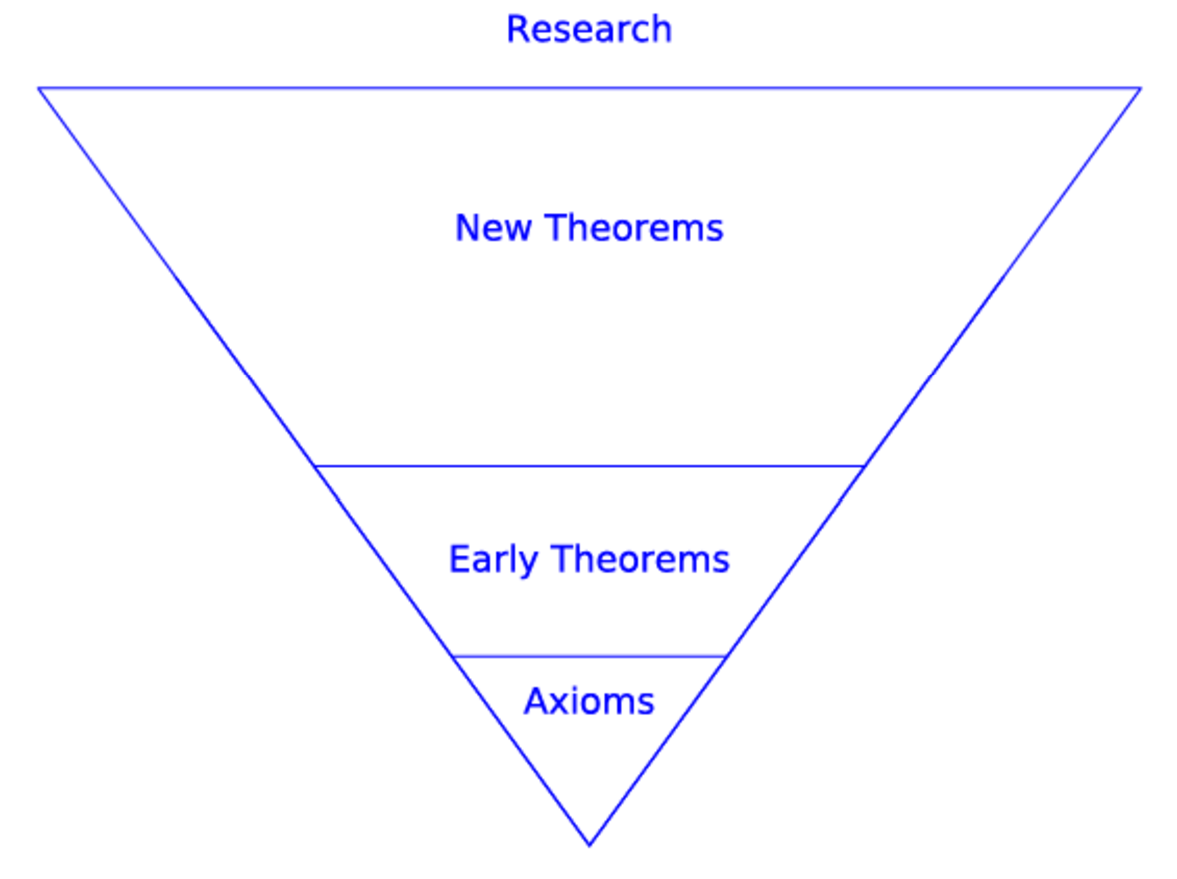
\includegraphics[width=\linewidth]{images/pyramid.pdf}}%
{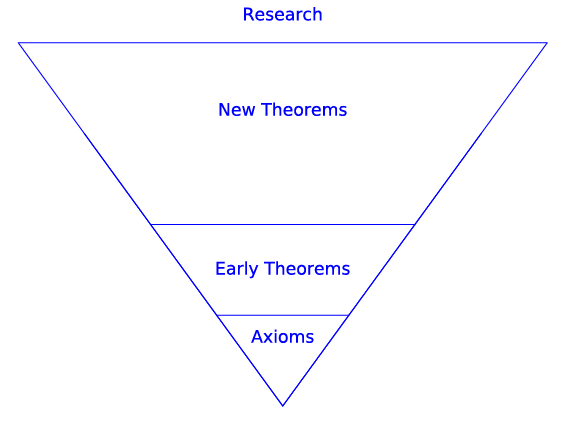
\includegraphics[width=\linewidth]{images/pyramid.png}}
\end{image}%
\tcblower
\end{figureptx}%
\begin{definition}{Proof.}{x:definition:def-proof}%
A proof of a theorem is a finite sequence of logically valid steps that demonstrate that the premises of a theorem imply its conclusion.%
\end{definition}
Exactly what constitutes a proof is not always clear. For example, a research mathematician might require only a few steps to prove a theorem to a colleague, but might take an hour to give an effective proof to a class of students. Therefore, what constitutes a proof often depends on the audience. But the audience is not the only factor. One of the most famous theorems in graph theory, \hyperref[x:theorem:theorem-four-color-theorem]{The Four-Color Theorem}, was proven in 1976, after over a century of effort by many mathematicians.  Part of the proof consisted of having a computer check many different graphs for a certain property. Without the aid of the computer, this checking would have taken years. In the eyes of some mathematicians, this proof was considered questionable. Shorter proofs have been developed since 1976 and there is no controversy associated with The Four Color Theorem at this time.%
\end{subsectionptx}
%
%
\typeout{************************************************}
\typeout{Subsection 3.5.2 Direct Proof}
\typeout{************************************************}
%
\begin{subsectionptx}{Direct Proof}{}{Direct Proof}{}{}{g:subsection:idm40460952736}
Theoretically, you can prove anything in propositional calculus with truth tables. In fact, the laws of logic stated in Section 3.4 are all theorems.  Propositional calculus is one of the few mathematical systems for which any valid sentence can be determined true or false by mechanical means. A program to write truth tables is not too difficult to write; however, what can be done theoretically is not always practical. For example,%
\begin{equation*}
a, a\to  b, b\to  c, . . . ,y\to z\Rightarrow z
\end{equation*}
is a theorem in propositional calculus. However, suppose that you wrote such a program and you had it write the truth table for%
\begin{equation*}
(a\land  (a\to  b)\land ( b\to  c)\land \cdots \land (y\to z))\to z
\end{equation*}
The truth table will have \(2^{26}\) cases. At one million cases per second, it would take approximately one hour to verify the theorem.  Now if you decided to check a similar theorem,%
\begin{equation*}
p_1,p_1\to p_2,\ldots  ,p_{99}\to p_{100}\Rightarrow p_{100}
\end{equation*}
you would really have time trouble. There would be \(2^{100} \approx 1.26765\times 10^{30}\) cases to check in the truth table.  At one million cases per second it would take approximately \(1.46719\times 10^{19}\) days to check all cases.  For most of the remainder of this section, we will discuss an alternate method for proving theorems in propositional calculus. It is the same method that we will use in a less formal way for proofs in other systems. Formal axiomatic methods would be too unwieldy to actually use in later sections. However, none of the theorems in later chapters would be stated if they couldn't be proven by the axiomatic method.%
\par
We will introduce two types of proof here, direct and indirect.%
\begin{example}{A typical direct proof.}{x:example:proof-3-5-1}%
\index{Direct proof}%
This is a theorem: \(p \rightarrow  r, q\rightarrow s,p\lor q\Rightarrow s\lor r\).   A direct proof of this theorem is:%
\begin{tableptx}{\textbf{Direct proof of \(p \rightarrow  r, q\rightarrow s,p\lor q\Rightarrow s\lor r\)}}{x:table:proof-steps-1}{}%
\centering
{\tabularfont%
\begin{tabular}{ccc}
Step&Proposition&Justification\tabularnewline[0pt]
1.&\(p \lor  q\)&Premise\tabularnewline[0pt]
2.&\(\neg p \rightarrow  q\)&(1), conditional rule\tabularnewline[0pt]
3.&\(q \rightarrow  s\)&Premise\tabularnewline[0pt]
4.&\(\neg p \rightarrow  s\)&(2), (3), chain rule\tabularnewline[0pt]
5.&\(\neg s \rightarrow p\)&(4), contrapositive\tabularnewline[0pt]
6.&\(p \rightarrow  r\)&Premise\tabularnewline[0pt]
7.&\(\neg s \rightarrow  r\)&(5), (6), chain rule\tabularnewline[0pt]
8.&\(s \lor r\)&(7), conditional rule   \(\square\)
\end{tabular}
}%
\end{tableptx}%
\end{example}
Note that \(\square\) marks the end of a proof.%
\par
\hyperref[x:example:proof-3-5-1]{Example~{\xreffont\ref{x:example:proof-3-5-1}}} illustrates the usual method of formal proof in a formal mathematical system. The rules governing these proofs are:%
\par
%
\begin{enumerate}[label=(\arabic*)]
\item{}A proof must end in a finite number of steps.%
\item{}Each step must be either a premise or a proposition that is implied from previous steps using any valid equivalence or implication.%
\item{}For a direct proof, the last step must be the conclusion of the theorem. For an indirect proof (see below), the last step must be a contradiction.%
\item{}Justification Column. The column labeled ``justification'' is analogous to the comments that appear in most good computer programs. They simply make the proof more readable.%
\end{enumerate}
%
\begin{example}{Two proofs of the same theorem.}{x:example:proof-3-5-2}%
Here are two direct proofs of \(\neg p \lor  q, s\lor  p, \neg q \Rightarrow  s\):%
\begin{tableptx}{\textbf{Direct proof of  \(\neg p \lor  q, s\lor  p, \neg q \Rightarrow  s\)}}{x:table:proof-steps-2}{}%
\centering
{\tabularfont%
\begin{tabular}{ccc}
1.&\(\neg p \lor  q\)&Premise\tabularnewline[0pt]
2.&\(\neg q\)&Premise\tabularnewline[0pt]
3.&\(\neg p\)&Disjunctive simplification, (1), (2)\tabularnewline[0pt]
4.&\(s\lor  p\)&Premise\tabularnewline[0pt]
5.&\(s\)&Disjunctive simplification, (3), (4). \(\square\)
\end{tabular}
}%
\end{tableptx}%
You are invited to justify the steps in this second proof:%
\begin{tableptx}{\textbf{Alternate  proof of  \(\neg p \lor  q, s\lor  p, \neg q \Rightarrow  s\)}}{x:table:proof-steps-2a}{}%
\centering
{\tabularfont%
\begin{tabular}{cc}
1.&\(\neg p \lor  q\)\tabularnewline[0pt]
2.&\(\neg q \rightarrow  \neg p\)\tabularnewline[0pt]
3.&\(s\lor p\)\tabularnewline[0pt]
4.&\(p \lor  s\)\tabularnewline[0pt]
5.&\(\neg p \to s\)\tabularnewline[0pt]
6.&\(\neg q \rightarrow  s\)\tabularnewline[0pt]
7.&\(\neg q\)\tabularnewline[0pt]
8.&\(s\)    \(\square\)
\end{tabular}
}%
\end{tableptx}%
\end{example}
The conclusion of a theorem is often a conditional proposition. The condition of the conclusion can be included as a premise in the proof of the theorem. The object of the proof is then to prove the consequence of the conclusion. This rule is justified by the logical law%
\begin{equation*}
p \rightarrow  (h \rightarrow  c) \Leftrightarrow  (p \land  h) \rightarrow  c
\end{equation*}
%
\begin{example}{Example of a proof with a conditional conclusion.}{x:example:ex-conditinal-conclusion}%
The following proof of \(p \to  (q \rightarrow  s), \neg r  \lor p, q \Rightarrow r \rightarrow s\) includes \(r\) as a fourth premise. Inference of truth of \(s\) completes the proof.%
\begin{tableptx}{\textbf{Proof of a theorem with a conditional conclusion.}}{x:table:proof-conditional-conclusion}{}%
\centering
{\tabularfont%
\begin{tabular}{ccc}
1.&\(\neg r \lor p\)&Premise\tabularnewline[0pt]
2.&\(r\)&Added premise\tabularnewline[0pt]
3.&\(p\)&(1), (2), disjunction simplification\tabularnewline[0pt]
4.&\(p \rightarrow  (q \to s)\)&Premise\tabularnewline[0pt]
5.&\(q\rightarrow s\)&(3), (4), detachment\tabularnewline[0pt]
6.&\(q\)&Premise\tabularnewline[0pt]
7.&\(s\)&(5), (6), detachment. \(\square\)
\end{tabular}
}%
\end{tableptx}%
\end{example}
\end{subsectionptx}
%
%
\typeout{************************************************}
\typeout{Subsection 3.5.3 Indirect Proof}
\typeout{************************************************}
%
\begin{subsectionptx}{Indirect Proof}{}{Indirect Proof}{}{}{x:subsection:sub-indirect-proof}
Consider a theorem \(P\Rightarrow C\), where \(P\) represents \(p_1, p_2, . . . , \textrm{ and } p_n\), the premises. The method of \terminology{indirect proof}\index{Indirect proof} is based on the equivalence \(P\rightarrow C\Leftrightarrow \neg (P\land  \neg C)\). In words, this logical law states that if \(P \Rightarrow  C\), then \(P \land  \neg  C\) is always false; that is, \(P \land  \neg C\) is a contradiction. This means that a valid method of proof is to negate the conclusion of a theorem and add this negation to the premises. If a contradiction can be implied from this set of propositions, the proof is complete. For the proofs in this section, a contradiction will often take the form \(t \land \neg t\).%
\par
For proofs involving numbers, a contradiction might be \(1 = 0\) or \(0 < 0\). Indirect proofs involving sets might conclude with \(x \in  \emptyset\) or (\(x \in  A\) and \(x \in  A^c\)). Indirect proofs are often more convenient than direct proofs in certain situations.  Indirect proofs are often called \emph{proofs by contradiction}.%
\begin{example}{An Indirect Proof.}{x:example:ex-indirect_proof_1}%
Here is an example of an indirect proof of the theorem in \hyperref[x:example:proof-3-5-1]{Example~{\xreffont\ref{x:example:proof-3-5-1}}}.%
\begin{tableptx}{\textbf{An Indirect proof of \(p \rightarrow  r, q\rightarrow s,p\lor q\Rightarrow s\lor r\)}}{x:table:proof-indirect}{}%
\centering
{\tabularfont%
\begin{tabular}{ccc}
1.&\(\neg (s \lor  r)\)&Negated conclusion\tabularnewline[0pt]
2.&\(\neg s \land  \neg r\)&DeMorgan's Law, (1)\tabularnewline[0pt]
3.&\(\neg s\)&Conjunctive simplification, (2)\tabularnewline[0pt]
4.&\(q\to s\)&Premise\tabularnewline[0pt]
5.&\(\neg q\)&Indirect reasoning, (3), (4)\tabularnewline[0pt]
6.&\(\neg r\)&Conjunctive simplification, (2)\tabularnewline[0pt]
7.&\(p \rightarrow  r\)&Premise\tabularnewline[0pt]
8.&\(\neg p\)&Indirect reasoning, (6), (7)\tabularnewline[0pt]
9.&\((\neg p) \land  (\neg q)\)&Conjunctive, (5), (8)\tabularnewline[0pt]
10.&\(\neg (p \lor  q)\)&DeMorgan's Law, (9)\tabularnewline[0pt]
11.&\(p \lor  q\)&Premise\tabularnewline[0pt]
12.&\(0\)&(10), (11) \(\square\)
\end{tabular}
}%
\end{tableptx}%
\end{example}
\begin{note}{Proof Style.}{g:note:idm40460888688}%
The rules allow you to list the premises of a theorem immediately; however, a proof is much easier to follow if the premises are only listed when they are needed.%
\end{note}
\begin{example}{Yet Another Indirect Proof.}{x:example:proof-yet-another}%
Here is an indirect proof of \(a \rightarrow  b, \neg (b \lor  c ) \Rightarrow  \neg  a\).%
\begin{tableptx}{\textbf{Indirect proof of \(a \rightarrow  b, \neg (b \lor  c ) \Rightarrow  \neg  a\)}}{x:table:proof-style}{}%
\centering
{\tabularfont%
\begin{tabular}{ccc}
1.&\(a\)&Negation of the conclusion\tabularnewline[0pt]
2.&\(a\to  b\)&Premise\tabularnewline[0pt]
3.&\(b\)&(1), (2), detachment\tabularnewline[0pt]
4.&\(b \lor  c\)&(3), disjunctive addition\tabularnewline[0pt]
5.&\(\neg (b \lor  c)\)&Premise\tabularnewline[0pt]
6.&\(0\)&(4), (5)  \(\square\)
\end{tabular}
}%
\end{tableptx}%
\end{example}
As we mentioned at the outset of this section, we are only presenting an overview of what a mathematical system is. For greater detail on axiomatic theories, see Stoll (1961). An excellent description of how propositional calculus plays a part in artificial intelligence is contained in Hofstadter (1980). If you enjoy the challenge of constructing proofs in propositional calculus, you should enjoy the game WFF'N PROOF (1962), by L.E. Allen.%
\end{subsectionptx}
%
%
\typeout{************************************************}
\typeout{Exercises 3.5.4 Exercises}
\typeout{************************************************}
%
\begin{exercises-subsection}{Exercises}{}{Exercises}{}{}{x:exercises:exercises-3-5}
\begin{divisionexercise}{1}{}{}{g:exercise:idm40460862704}%
Prove with truth tables:%
\par
%
\begin{enumerate}[label=(\alph*)]
\item{}\(p\lor  q, \neg q\Rightarrow  p\)%
\item{}\(p \rightarrow  q, \neg q \Rightarrow  \neg p\)%
\end{enumerate}
%
\end{divisionexercise}%
\begin{divisionexercise}{2}{}{}{g:exercise:idm40460858640}%
Prove with truth tables:%
\par
%
\begin{enumerate}[label=(\alph*)]
\item{}\(q, \neg q\Rightarrow  p\)%
\item{}\(p \rightarrow  q \Rightarrow  \neg p \lor  q\)%
\end{enumerate}
%
\end{divisionexercise}%
\begin{divisionexercise}{3}{}{}{g:exercise:idm40460854336}%
Give direct and indirect proofs of:%
\par
%
\begin{enumerate}[label=(\alph*)]
\item{}\(a \rightarrow  b, c \rightarrow  b, d\rightarrow  (a \lor  c), d\Rightarrow  b\).%
\item{}\((p\to q) \land (r\to s), (q\rightarrow t) \land  (s \to  u), \neg (t \land u), p \rightarrow  r \Rightarrow  \neg p\).%
\item{}\(p\to (q\to r),\neg s \lor p,q\Rightarrow s\to r\).%
\item{}\(p\rightarrow  q, q\rightarrow  r, \neg (p \land  r), p \lor  r \Rightarrow  r\).%
\item{}\(\neg q, p\to q, p\lor t \Rightarrow t\)%
\end{enumerate}
%
\end{divisionexercise}%
\begin{divisionexercise}{4}{}{}{g:exercise:idm40460770912}%
Give direct and indirect proofs of:%
\par
%
\begin{enumerate}[label=(\alph*)]
\item{}\(p\rightarrow  q, \neg r\rightarrow  \neg q, \neg r \Rightarrow  \neg p\).%
\item{}\(p\rightarrow  \neg q, \neg r\rightarrow  q, p \Rightarrow  r\).%
\item{}\(a \lor  b, c \land  d, a \rightarrow  \neg c \Rightarrow  b\).%
\end{enumerate}
%
\end{divisionexercise}%
\begin{divisionexercise}{5}{}{}{g:exercise:idm40460767312}%
Are the following arguments valid? If they are valid, construct formal proofs; if they aren't valid, explain why not.%
\par
%
\begin{enumerate}[label=(\alph*)]
\item{}If wages increase, then there will be inflation. The cost of living will not increase if there is no inflation. Wages will increase. Therefore, the cost of living will increase.%
\item{}If the races are fixed or the casinos are crooked, then the tourist trade will decline. If the tourist trade decreases, then the police will be happy. The police force is never happy. Therefore, the races are not fixed.%
\end{enumerate}
%
\end{divisionexercise}%
\begin{divisionexercise}{6}{}{}{g:exercise:idm40488393984}%
Determine the validity of the following argument: For students to do well in a discrete mathematics course, it is necessary that they study hard. Students who do well in courses do not skip classes. Students who study hard do well in courses. Therefore students who do well in a discrete mathematics course do not skip class.%
\end{divisionexercise}%
\begin{divisionexercise}{7}{}{}{g:exercise:idm40474493088}%
Describe how \(p_1,p_1\to p_2,\ldots  ,p_{99}\to p_{100}\Rightarrow p_{100}\) could be proved in 199 steps.%
\end{divisionexercise}%
\end{exercises-subsection}
\end{sectionptx}
%
%
\typeout{************************************************}
\typeout{Section 3.6 Propositions over a Universe}
\typeout{************************************************}
%
\begin{sectionptx}{Propositions over a Universe}{}{Propositions over a Universe}{}{}{x:section:s-propositions-over-universe}
%
%
\typeout{************************************************}
\typeout{Subsection 3.6.1 Propositions over a Universe}
\typeout{************************************************}
%
\begin{subsectionptx}{Propositions over a Universe}{}{Propositions over a Universe}{}{}{x:subsection:ss-propositions-over-a-universe}
Consider the sentence ``He was a member of the Boston Red Sox.'' There is no way that we can assign a truth value to this sentence unless ``he'' is specified. For that reason, we would not consider it a proposition. However, ``he'' can be considered a variable that holds a place for any name. We might want to restrict the value of ``he'' to all names in the major-league baseball record books. If that is the case, we say that the sentence is a proposition over the set of major-league baseball players, past and present.%
\begin{definition}{Proposition over a Universe.}{x:definition:def-proposition-over-U}%
Let \(U\) be a nonempty set. A proposition over \(U\) is a sentence that contains a variable that can take on any value in \(U\) and that has a definite truth value as a result of any such substitution.%
\end{definition}
\begin{example}{Some propositions over a variety of universes.}{x:example:ex-some-propositions-over-U}%
%
\begin{enumerate}[label=(\alph*)]
\item{}A few propositions over the integers are \(4x^2 - 3x = 0\),  \(0 \leq  n \leq 5\), and ``\(k\) is a multiple of 3.''%
\item{}A few propositions over the rational numbers are \(4x^2 - 3x = 0\),  \(y^2=2\), and  \((s - 1)(s + 1) = s^2 - 1\).%
\item{}A few propositions over the subsets of \(\mathbb{P}\) are \((A =\emptyset ) \lor  (A = \mathbb{P} )\), \(3 \in  A\), and  \(A \cap  \{1, 2, 3\}\neq  \emptyset\).%
\end{enumerate}
%
\end{example}
All of the laws of logic that we listed in Section 3.4 are valid for propositions over a universe. For example, if \(p\) and \(q\) are propositions over the integers, we can be certain that \(p \land  q \Rightarrow  p\), because \((p \land  q) \to  p\) is a tautology and is true no matter what values the variables in \(p\) and \(q\) are given. If we specify \(p\) and \(q\) to be \(p(n) : n < 4\) and \(q(n) : n < 8\), we can also say that \(p\) implies \(p \land  q\). This is not a usual implication, but for the propositions under discussion, it is true. One way of describing this situation in general is with truth sets.%
\end{subsectionptx}
%
%
\typeout{************************************************}
\typeout{Subsection 3.6.2 Truth Sets}
\typeout{************************************************}
%
\begin{subsectionptx}{Truth Sets}{}{Truth Sets}{}{}{x:subsection:ss-truth-sets}
\begin{definition}{Truth Set.}{x:definition:def-truth-set}%
\index{Truth Set}%
\label{g:notation:idm40472291488}%
If \(p\) is a proposition over \(U\), the truth set of \(p\) is \(T_p = \{a \in  U \mid p(a) \textrm{ is true}\}\).%
\end{definition}
\begin{example}{Truth Set Example.}{x:example:ex-set-prop}%
The truth set of the proposition \(\{1, 2\} \cap A = \emptyset\), taken as a proposition over the power set of \(\{1, 2, 3, 4\}\) is \(\{\emptyset , \{3\}, \{4\}, \{3, 4\}\}\).%
\end{example}
\begin{example}{Truth sets depend on the universe.}{x:example:ex-vary-U}%
Over the universe \(\mathbb{Z}\) (the integers), the truth set of \(4x^2- 3x = 0\) is \(\{0\}\). If the universe is expanded to the rational numbers, the truth set becomes \(\{0, 3/4\}\). The term \emph{solution set} is often used for the truth set of an equation such as the one in this example.%
\end{example}
\begin{definition}{Tautologies and Contradictions over a Universe.}{x:definition:def-tautology-contradiction-over-U}%
A proposition over \(U\) is a tautology if its truth set is \(U\). It is a contradiction if its truth set is empty.%
\end{definition}
\begin{example}{Tautology, Contradiction over \(\mathbb{Q}\).}{x:example:ex-tautology-contradiction-over-U}%
\((s - 1)(s + 1) = s^2 - 1\) is a tautology over the rational numbers. \(x^2-2 = 0\) is a contradiction over the rationals.%
\end{example}
The truth sets of compound propositions can be expressed in terms of the truth sets of simple propositions. For example, if \(a \in  T_{p\land q}\) if and only if \(a\) makes \(p \land  q\) true. This is true if and only if  \(a\) makes both \(p\) and \(q\) true,  which, in turn, is true if and only if  \(a \in  T_p\cap T_q\). This explains why the truth set of the conjunction of two propositions equals the intersection of the truth sets of the two propositions. The following list summarizes the connection between compound and simple truth sets%
\begin{tableptx}{\textbf{Truth Sets of Compound Statements}}{x:table:table-truth-sets-compound-statements}{}%
\centering
{\tabularfont%
\begin{tabular}{c}
\(T_{p\land q}=T_p\cap T_q\)\tabularnewline[0pt]
\(T_{p\lor q}=T_p\cup T_q\)\tabularnewline[0pt]
\(T_{\neg p}=T_p{}^c\)\tabularnewline[0pt]
\(T_{p\leftrightarrow q}=\left(T_p\cap T_q\right)\cup \left(T_p{}^c\cap T_q{}^c\right)\)\tabularnewline[0pt]
\(T_{p\to q}=T_p{}^c\cup T_q\)
\end{tabular}
}%
\end{tableptx}%
\begin{definition}{Equivalence of propositions over a universe.}{x:definition:def-equivanlence-over-U}%
Two propositions, \(p\) and \(q\), are equivalent if \(p \leftrightarrow  q\) is a tautology. In terms of truth sets, this means that \(p\) and \(q\) are equivalent if \(T_p=T_q\) .%
\end{definition}
\begin{example}{Some pairs of equivalent propositions.}{x:example:ex-some-equivalent-pairs}%
%
\begin{enumerate}[label=(\alph*)]
\item{}\(n + 4 = 9\) and \(n = 5\) are equivalent propositions over the integers.%
\item{}\(A \cap  \{4\} \neq  \emptyset\) and \(4 \in  A\) are equivalent propositions over the power set of the natural numbers.%
\end{enumerate}
%
\end{example}
\begin{definition}{Implication for propositions over a universe.}{x:definition:def-implication-over-U}%
If \(p\) and \(q\) are propositions over \(U\), \(p\) implies \(q\) if \(p \rightarrow q\) is a tautology.%
\end{definition}
Since the truth set of \(p \rightarrow  q\) is \(T_p{}^c\cup T_q\), the Venn diagram for \(T_{p\to q}\) in \hyperref[x:figure:venn_diagram_truth_set_conditional]{Figure~12} shows that \(p \Rightarrow  q\) when \(T_p\subseteq T_q\).%
\begin{figureptx}{Venn Diagram for \(T_{p\to q}\)}{x:figure:venn_diagram_truth_set_conditional}{}%
\begin{image}{0.15}{0.7}{0.15}%
\IfFileExists{images/sageplot-venn-truth-set-conditional.pdf}%
{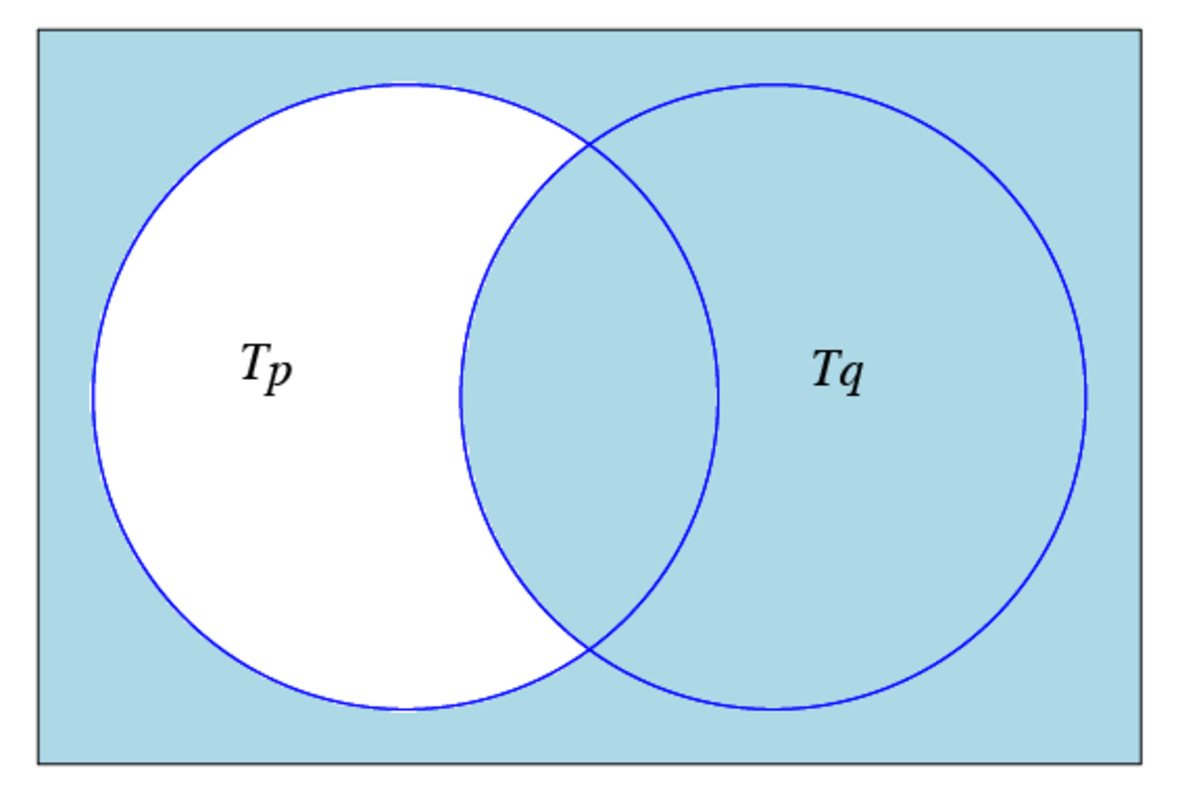
\includegraphics[width=\linewidth]{images/sageplot-venn-truth-set-conditional.pdf}}%
{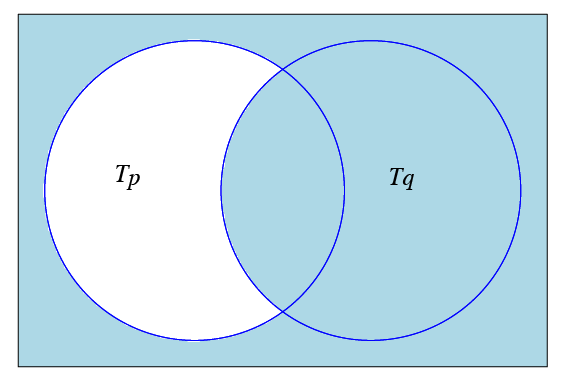
\includegraphics[width=\linewidth]{images/sageplot-venn-truth-set-conditional.png}}
\end{image}%
\tcblower
\end{figureptx}%
\begin{example}{Examples of Implications.}{x:example:ex-implications-over-U}%
%
\begin{enumerate}[label=(\alph*)]
\item{}Over the natural numbers: \(n \leq 4 \Rightarrow  n \leq 8\) since \(\{0, 1, 2, 3, 4\} \subseteq  \{0, 1, 2, 3, 4, 5, 6, 7, 8\}\)%
\item{}Over the power set of the integers: \(\lvert A^c \rvert=1\) implies \(A\cap \{0,1\}\neq \emptyset\)%
\item{}Over the power set of the integers,  \(A \subseteq  \textrm{ even integers } \Rightarrow  A\cap  \textrm{ odd integers } =\emptyset\)%
\end{enumerate}
%
\end{example}
\end{subsectionptx}
%
%
\typeout{************************************************}
\typeout{Exercises 3.6.3 Exercises}
\typeout{************************************************}
%
\begin{exercises-subsection}{Exercises}{}{Exercises}{}{}{x:exercises:exercises-3-6}
\begin{divisionexercise}{1}{}{}{g:exercise:idm40474104832}%
If \(U = \mathcal{P}( \{1, 2, 3, 4\})\), what are the truth sets of the following propositions?%
\par
%
\begin{enumerate}[label=(\alph*)]
\item{}\(A \cap  \{2, 4\} = \emptyset\).%
\item{}\(3 \in  A\) and \(1 \notin  A\).%
\item{}\(A \cup  \{1\} = A\).%
\item{}\(A\) is a proper subset of \(\{2, 3, 4\}\).%
\item{}\(\lvert A \rvert=\lvert A^c \rvert\).%
\end{enumerate}
%
\end{divisionexercise}%
\begin{divisionexercise}{2}{}{}{g:exercise:idm40474106768}%
Over the universe of positive integers, define%
\begin{tableptx}{\textbf{}}{g:table:idm40474190080}{}%
\centering
{\tabularfont%
\begin{tabular}{ll}
\(p(n)\):&\(n\) is prime and \(n < 32\).\tabularnewline[0pt]
\(q(n)\):&\(n\) is a power of 3.\tabularnewline[0pt]
\(r(n)\):&\(n\) is a divisor of 27.
\end{tabular}
}%
\end{tableptx}%
%
\begin{enumerate}[label=(\alph*)]
\item{}What are the truth sets of these propositions?%
\item{}Which of the three propositions implies one of the others?%
\end{enumerate}
%
\end{divisionexercise}%
\begin{divisionexercise}{3}{}{}{g:exercise:idm40474160192}%
If \(U = \{0, 1, 2\}\), how many propositions over \(U\) could you list without listing two that are equivalent?%
\end{divisionexercise}%
\begin{divisionexercise}{4}{}{}{g:exercise:idm40474244912}%
Given the propositions over the natural numbers:%
\begin{tableptx}{\textbf{}}{g:table:idm40474324816}{}%
\centering
{\tabularfont%
\begin{tabular}{lll}
\(p : n < 4\),&\(q : 2n > 17\), and&\(r : n \textrm{ is  a  divisor of } 18\)
\end{tabular}
}%
\end{tableptx}%
What are the truth sets of:%
\begin{multicols}{2}
\begin{enumerate}[label=(\alph*)]
\item{}\(q\)%
\item{}\(p\land q\)%
\item{}\(r\)%
\item{}\(q\to r\)%
\end{enumerate}
\end{multicols}
%
\end{divisionexercise}%
\begin{divisionexercise}{5}{}{}{g:exercise:idm40474302160}%
Suppose that \(s\) is a proposition over \(\{1, 2,\dots, 8\}\). If \(T_s = \{1, 3, 5, 7\}\), give two examples of propositions that are equivalent to \(s\).%
\end{divisionexercise}%
\begin{divisionexercise}{6}{}{}{g:exercise:idm40474398240}%
%
\begin{enumerate}[label=(\alph*)]
\item{}Determine the truth sets of the following propositions over the positive integers:%
\begin{equation*}
p(n) : n \textrm{ is a perfect square and }  n < 100
\end{equation*}
%
\begin{equation*}
q(n) : n = \lvert \mathcal{P}(A) \rvert \textrm{ for some set } A\text{.}
\end{equation*}
%
\item{}Determine \(T_{p\land q}\) for \(p\) and \(q\) above.%
\end{enumerate}
%
\end{divisionexercise}%
\begin{divisionexercise}{7}{}{}{g:exercise:idm40474402368}%
Let the universe be \(\mathbb{Z}\), the set of integers. Which of the following propositions are equivalent over \(\mathbb{Z}\)?%
\begin{tableptx}{\textbf{}}{g:table:idm40474440752}{}%
\centering
{\tabularfont%
\begin{tabular}{ll}
\(a\):&\(0 < n^2 < 9\)\tabularnewline[0pt]
\(b\):&\(0 < n^3 < 27\)\tabularnewline[0pt]
\(c\):&\(0 < n < 3\)
\end{tabular}
}%
\end{tableptx}%
\end{divisionexercise}%
\end{exercises-subsection}
\end{sectionptx}
%
%
\typeout{************************************************}
\typeout{Section 3.7 Mathematical Induction}
\typeout{************************************************}
%
\begin{sectionptx}{Mathematical Induction}{}{Mathematical Induction}{}{}{x:section:s-induction}
%
%
\typeout{************************************************}
\typeout{Subsection 3.7.1 Introduction, First Example}
\typeout{************************************************}
%
\begin{subsectionptx}{Introduction, First Example}{}{Introduction, First Example}{}{}{g:subsection:idm40474509760}
In this section, we will examine mathematical induction, a technique for proving propositions over the positive integers. Mathematical induction reduces the proof that all of the positive integers belong to a truth set to a finite number of steps.%
\begin{example}{Formula for Triangular Numbers.}{x:example:ex-triangular-numbers}%
Consider the following proposition over the positive integers, which we will label \(p(n)\): The sum of the positive integers from 1 to \(n\) is \(\frac{n (n+1)}{2}\). This is a well-known formula that is quite simple to verify for a given value of \(n\).   For example, \(p(5)\) is: The sum of the positive integers from 1 to 5 is \(\frac{5 (5+1)}{2}\). Indeed, \(1 + 2 + 3 + 4 + 5= 15 =\frac{5(5+1)}{2}\). However, this doesn't serve as a proof that \(p(n)\) is a tautology. All that we've established is that \(5\) is in the truth set of \(p\). Since the positive integers are infinite, we certainly can't use this approach to prove the formula.%
\end{example}
\emph{An Analogy}: A proof by mathematical induction is similar to knocking over a row of closely spaced dominos that are standing on end. To knock over the dominos in \hyperref[x:figure:dominos]{Figure~{\xreffont\ref{x:figure:dominos}}}, all you need to do is push the first domino over. To be assured that they all will be knocked over, some work must be done ahead of time. The dominos must be positioned so that if any domino is pushed is knocked over, it will push the next domino in the line.%
\begin{figureptx}{An analogy for Mathematical Induction, Creative Commons photo by Ranveig Thattai}{x:figure:dominos}{}%
\begin{image}{0.15}{0.7}{0.15}%
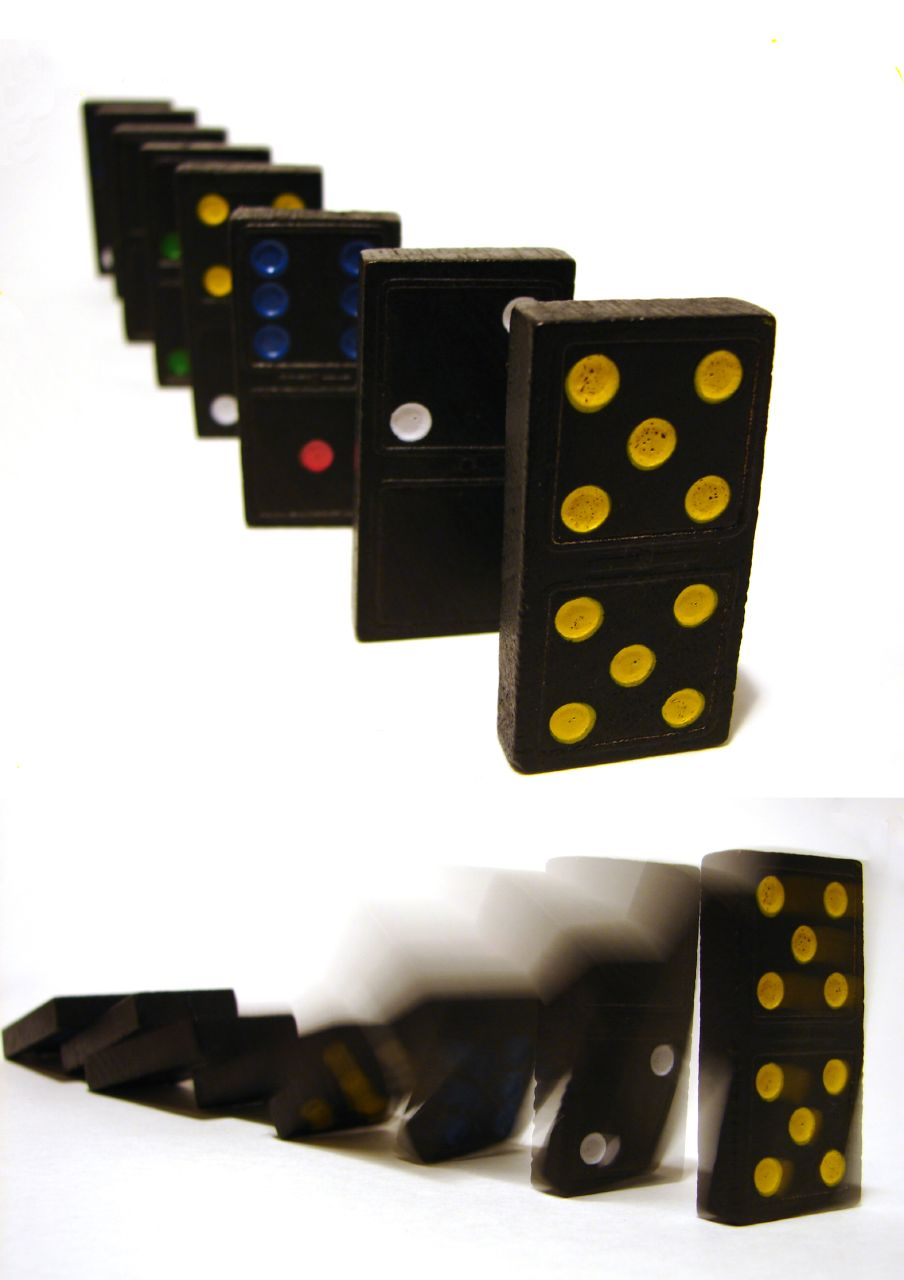
\includegraphics[width=\linewidth]{images/Domino_effect.png}
\end{image}%
\tcblower
\end{figureptx}%
Returning to  \hyperref[x:example:ex-triangular-numbers]{Example~{\xreffont\ref{x:example:ex-triangular-numbers}}} imagine the propositions \(p(1), p(2), p(3),\ldots\) to be an infinite line of dominos. Let's see if these propositions are in the same formation as the dominos were.  First, we will focus on one specific point of the line: \(p(99)\) and \(p(100)\). We are not going to prove that either of these propositions is true, just that the truth of \(p(99)\) implies the truth of \(p(100)\). In terms of our analogy, if \(p(99)\) is knocked over, it will knock over \(p(100)\).%
\par
In proving \(p(99) \Rightarrow  p(100)\), we will use \(p(99)\) as our premise. We must prove: The sum of the positive integers from 1 to 100 is \(\frac{100 (100+1)}{2}\). We start by observing that the sum of the positive integers from 1 to 100 is \((1 + 2 + \cdots  + 99) +100\). That is, the sum of the positive integers from 1 to 100 equals  the sum of the first ninety-nine plus the final number, 100. We can now apply our premise, \(p(99)\), to the sum \(1 + 2 + \cdots  + 99\). After rearranging our numbers, we obtain the desired expression for \(1 + 2 + \cdots  + 100\):%
\begin{equation*}
\begin{split}
1 + 2 + \cdots  + 99 + 100 & = (1 + 2 + \cdots + 99) + 100 \\ 
& = \frac{99\cdot (99+1)}{2}+ 100 \textrm{         by our assumption of } p(99)\\
& = \frac{99\cdot 100}{2} + \frac{2\cdot 100}{2} \\
& =  \frac{100\cdot 101}{2}  \\
& = \frac{100\cdot (100+1)}{2} 
\end{split}\text{.}
\end{equation*}
%
\par
What we've just done is analogous to checking two dominos in a line and finding that they are properly positioned. Since we are dealing with an infinite line, we must check all pairs at once. This is accomplished by proving that \(p(n) \Rightarrow  p(n + 1)\) for all \(n \geq  1\):%
\begin{equation*}
\begin{split}
1 + 2 + \cdots  + n + (n+1) & = (1 + 2 + \cdots  + n) + (n + 1) \\ 
& = \frac{ n(n+1)}{2} + (n + 1) \textrm{      by } p(n) \\
& =  \frac{ n(n+1)}{2}+\frac{2 (n+1)}{2}\\
& = \frac{  (n+1) (n+2)}{2}  \\
& = \frac{ (n+1) ((n+1)+1)}{2} 
\end{split}\text{.}
\end{equation*}
%
\par
They are all lined up! Now look at \(p(1)\): The sum of the positive integers from 1 to 1 is \(\frac{1\cdot(1+1)}{2}\). Clearly, \(p(1)\) is true. This sets off a chain reaction. Since \(p(1) \Rightarrow  p(2)\), \(p(2)\) is true. Since \(p(2) \Rightarrow  p(3)\), \(p(3)\) is true; and so on.   \(\blacksquare\)%
\begin{theorem}{The Principle of Mathematical Induction.}{}{x:theorem:th-math-induction-basic}%
Let \(p(n)\) be a proposition over the positive integers.  If%
\begin{enumerate}[label=(\arabic*)]
\item{}\(p(1)\) is true, and%
\item{}for all \(n\geq 1\),  \(p(n) \Rightarrow  p(n + 1)\),%
\end{enumerate}
then \(p(n)\) is a tautology.%
\end{theorem}
Note: The truth of \(p(1)\) is called the \emph{basis} for the induction proof. The premise that \(p(n)\) is true in the second part is called the \emph{induction hypothesis}.  The proof that \(p(n)\) implies \(p(n + 1)\) is called the \emph{induction  step} of the proof. Despite our analogy, the basis is usually done first in an induction proof. However, order doesn't really matter.%
\end{subsectionptx}
%
%
\typeout{************************************************}
\typeout{Subsection 3.7.2 More Examples}
\typeout{************************************************}
%
\begin{subsectionptx}{More Examples}{}{More Examples}{}{}{g:subsection:idm40472811344}
\begin{example}{Generalized Detachment.}{x:example:ex-logic-detachment}%
Consider the implication over the positive integers.%
\begin{equation*}
p(n): q_0 \rightarrow  q_1, q_1\to q_2, \ldots  , q_{n-1}\to q_n, q_0\Rightarrow  q_n
\end{equation*}
A proof that \(p(n)\) is a tautology follows. Basis: \(p(1)\) is \(q_0 \rightarrow  q_1, q_0\Rightarrow  q_1\). This is the logical law of detachment which we know is true. If you haven't done so yet, write out the truth table of \(((q_0 \rightarrow  q_1 )\land  q_0)\to  q_1\) to verify this step.%
\par
Induction: Assume that  \(p(n)\) is true for some \(n \geq  1\). We want to prove that \(p(n + 1)\) must be true. That is:%
\begin{equation*}
q_0 \rightarrow  q_1, q_1\to q_2, \ldots  , q_{n-1}\to q_n , q_n\to q_{n+1}, q_0\Rightarrow  q_{n+1}
\end{equation*}
Here is a direct proof of \(p(n + 1)\):%
\begin{tableptx}{\textbf{}}{x:table:table-general-detachment}{}%
\centering
{\tabularfont%
\begin{tabular}{ccc}
Step&Proposition&Justification\tabularnewline[0pt]
\(1 -(n+1)\)&\(q_0 \rightarrow  q_1, q_1\to q_2, \ldots  , q_{n-1}\to q_n, q_0\)&Premises\tabularnewline[0pt]
\(n+2\)&\(q_n\)&\((1)-(n+1)\), \(p(n)\)\tabularnewline[0pt]
\(n+3\)&\(q_n\to q_{n+1}\)&Premise\tabularnewline[0pt]
\(n+4\)&\(q_{n+1}\)&\((n+2),(n+3), \textrm{ detachment} \quad \square\)
\end{tabular}
}%
\end{tableptx}%
\end{example}
\begin{example}{An example from Number Theory.}{x:example:ex-number-theory-3s}%
For all \(n \geq  1\), \(n^3+2n\)  is a multiple of 3.  An inductive proof follows:%
\par
Basis:  \(1^3+2(1)= 3\) is a multiple of 3. The basis is almost always this easy!%
\par
Induction: Assume that \(n \geq  1\) and \(n^3+2n\) is a multiple of 3. Consider \((n+1)^3+2(n+1)\). Is it a multiple of 3?%
\par
%
\begin{equation*}
\begin{split}
(n+1)^3+2(n+1) & = n^3+3 n^2+3 n+1+ (2n+2) \\ 
& = n^3+2 n + 3 n^2+3 n+3  \\
& = (n^3+2 n) + 3( n^2+ n+1)
\end{split}\text{.}
\end{equation*}
%
\par
Yes, \((n+1)^3+2(n+1)\) is the sum of two multiples of 3; therefore, it is also a multiple of 3.  \(\square\)%
\end{example}
Now we will discuss some of the variations of the principle of mathematical induction. The first simply allows for universes that are similar to \(\mathbb{P}\) such as \(\{-2, -1, 0, 1,\ldots \}\) or \(\{5, 6, 7, 8,\ldots \}\).%
\begin{theorem}{Principle of Mathematical Induction (Generalized).}{}{x:theorem:th-math-induction-generalized}%
If \(p(n)\) is a proposition over \(\{k_0 , k_0+ 1, k_0+ 2,\ldots  \}\), where \(k_0\) is any integer, then \(p(n)\) is a tautology if%
\par
%
\begin{enumerate}[label=(\arabic*)]
\item{}\(p(k_0)\) is true, and%
\item{}for all \(n \geq k_0\),  \(p(n) \Rightarrow  p(n + 1)\).%
\end{enumerate}
%
\end{theorem}
\begin{example}{A proof of the permutations formula.}{x:example:ex-permuations-formula-proof}%
In Chapter 2, we stated that the number of different permutations of \(k\) elements taken from an \(n\) element set, \(P(n; k)\), can be computed with the formula \(\frac{n!}{(n-k)!}\). We can prove this statement by induction on \(n\). For \(n \geq  0\), let \(q(n)\) be the proposition%
\begin{equation*}
P(n; k) = \frac{n!}{(n-k)!} \textrm{  for all } k \textrm{, } 0 \le k \le n\text{.}
\end{equation*}
%
\par
Basis: \(q(0)\) states that  \(P(0; 0) \) if is the number of ways that \(0\) elements can be selected from the empty set and arranged in order, then \(P(0; 0) = \frac{0!}{0!} = 1 \).  This is true. A general law in combinatorics is that there is exactly one way of doing nothing.%
\par
Induction: Assume that \(q(n)\) is true for some natural number \(n\). It is left for us to prove that this assumption implies that \(q(n +1)\) is true. Suppose that we have a set of cardinality \(n + 1\) and want to select and arrange \(k\) of its elements. There are two cases to consider, the first of which is easy. If \(k = 0\), then there is one way of selecting zero elements from the set; hence%
\begin{equation*}
P(n + 1; 0) = 1 =\frac{(n+1)!}{(n+1+0)!}
\end{equation*}
and the formula works in this case.%
\par
The more challenging case is to verify the formula when \(k\) is positive and less than or equal to \(n+1\). Here we count the value of \(P(n+ 1; k)\) by counting the number of ways that the first element in the arrangement can be filled and then counting the number of ways that the remaining \(k -1\) elements can be filled in using the induction hypothesis.%
\par
There are \(n + 1\) possible choices for the first element. Since that leaves \(n\) elements to fill in the remaining \(k - 1\) positions, there are \(P(n; k - 1)\) ways of completing the arrangement. By the rule of products,%
\begin{equation*}
\begin{split}
P(n +1;k) &= (n+1) P(n;k-1) \\
& = (n+1) \frac{n!}{(n-(k-1))!} \\
& = \frac{(n+1) n!}{(n-k+1)!}\\
& = \frac{(n+1)!}{((n+1)-k)!}
\end{split}
\end{equation*}
\(\blacksquare\)%
\end{example}
\end{subsectionptx}
%
%
\typeout{************************************************}
\typeout{Subsection 3.7.3 Course of Values Induction}
\typeout{************************************************}
%
\begin{subsectionptx}{Course of Values Induction}{}{Course of Values Induction}{}{}{g:subsection:idm40473467600}
A second variation allows for the expansion of the induction hypothesis. The course-of-values principle includes the previous generalization.  It is also sometimes called \emph{strong induction}.%
\begin{theorem}{The Course-of-Values Principle of Mathematical Induction.}{}{x:theorem:th-math-induction-course-of-values}%
If \(p(n)\) is a proposition over \(\{k_0 , k_0+ 1, k_0+ 2,\ldots  \}\), where \(k_0\) is any integer, then \(p(n)\) is a tautology if%
\par
%
\begin{enumerate}[label=(\arabic*)]
\item{}\(p(k_0)\) is true, and%
\item{}for all \(n\geq k_0\),   \(p(k_0), p(k_0 + 1), . . . , p(n) \Rightarrow  p(n + 1) \).%
\end{enumerate}
%
\end{theorem}
A prime number is defined as a positive integer that has exactly two positive divisors, 1 and itself. There are an infinite number of primes. The list of primes starts with \(2, 3, 5, 7, 11,\ldots \) .  The proposition over \(\{2, 3, 4, . . .\}\)  that we will prove here is \(p(n)\): \(n\) can be written as the product of one or more primes.  In most texts, the assertion that \(p(n)\) is a tautology would appear as%
\begin{theorem}{Existence of Prime Factorizations.}{}{x:theorem:th-prime-factorizations-exist}%
Every positive integer greater than or equal to 2 has a prime decomposition.%
\end{theorem}
\begin{proof}{}{g:proof:idm40473612960}
If you were to encounter this theorem outside the context of a discussion of mathematical induction, it might not be obvious that the proof can be done by induction. Recognizing when an induction proof is appropriate is mostly a matter of experience. Now on to the proof!%
\par
Basis:  Since 2 is a prime, it is already decomposed into primes (one of them).%
\par
Induction:  Suppose that for some \(n \geq  2\) all of the integers \(2,3, . . . , n\) have a prime decomposition.  Notice the course-of-value hypothesis.  Consider \(n + 1\). Either \(n + 1\) is prime or it isn't.   If \(n + 1\) is prime, it is already decomposed into primes. If not, then \(n + 1\) has a divisor, \(d\), other than 1 and \(n + 1\). Hence, \(n + 1 = c d\) where both \(c\) and \(d\) are between 2 and \(n\). By the induction hypothesis, \(c\) and \(d\) have prime decompositions, \(c_1 c_2 \cdots  c_s\) and \(d_1 d_2 \cdots d_t\) , respectively. Therefore, \(n + 1\) has the prime decomposition \(c_1 c_2 \cdots  c_s d_1 d_2 \cdots  d_t\).%
\end{proof}
\begin{historical}{Peano Postulates and Induction.}{x:historical:history-peano}%
Mathematical induction originated in the late nineteenth century. Two mathematicians who were prominent in its development were Richard Dedekind and Giuseppe Peano. Dedekind developed a set of axioms that describe the positive integers. Peano refined these axioms and gave a logical interpretation to them. The axioms are usually called the Peano Postulates.%
\end{historical}
\begin{axiom}{Peano Postulates.}{}{x:axiom:sss-peano-postulates}%
The system of positive integers consists of a nonempty set, \(\mathbb{P}\); a least element of \(\mathbb{P}\), denoted 1; and a ``successor function,'' s, with the properties%
\par
%
\begin{enumerate}[label=(\arabic*)]
\item{}If \(k \in  \mathbb{P}\) , then there is an element of \(\mathbb{P}\) called the successor of \(k\), denoted \(s(k)\).%
\item{}No two elements of \(\mathbb{P}\) have the same successor.%
\item{}No element of \(\mathbb{P}\) has \(1\) as its successor.%
\item{}If \(S \subseteq  \mathbb{P}\), \(1 \in  S\), and \(k \in S \Rightarrow  s(k) \in  S\), then \(S = \mathbb{P}\).%
\end{enumerate}
%
\end{axiom}
Notes:%
\par
%
\begin{itemize}[label=\textbullet]
\item{}You might recognize \(s(k)\) as simply being \(k + 1\).%
\item{}Axiom 4 is the one that makes mathematical induction possible. In an induction proof, we simply apply that axiom to the truth set of a proposition.%
\end{itemize}
%
\end{subsectionptx}
%
%
\typeout{************************************************}
\typeout{Exercises 3.7.4 Exercises}
\typeout{************************************************}
%
\begin{exercises-subsection}{Exercises}{}{Exercises}{}{}{x:exercises:exercises-3-7}
\begin{divisionexercise}{1}{}{}{g:exercise:idm40465593040}%
Prove that the sum of the first \(n\) odd integers equals \(n^2\) .%
\end{divisionexercise}%
\begin{divisionexercise}{2}{}{}{g:exercise:idm40465666144}%
Prove that if \(n \geq  1\), then \(1(1!) + 2(2!) + \cdots  + n(n!) = (n + 1)! - 1\).%
\end{divisionexercise}%
\begin{divisionexercise}{3}{}{}{g:exercise:idm40465715632}%
Prove that for \(n \geq  1\): \(\sum_{k=1}^n k^2= \frac{1}{6} n(n+1) (2 n+1)\).%
\end{divisionexercise}%
\begin{divisionexercise}{4}{}{}{g:exercise:idm40465748096}%
Prove that for \(n \geq  0\): \(\sum_{k=0}^n 2^k = 2^{n+1}-1\).%
\end{divisionexercise}%
\begin{divisionexercise}{5}{}{}{g:exercise:idm40465783920}%
Use mathematical induction to show that for \(n\geq 1\),%
\begin{equation*}
\frac{1}{1\cdot 2 }+ \frac{1}{2\cdot 3}+ \cdots  + \frac{1}{n(n+1)}= \frac{n}{n+1}\text{.}
\end{equation*}
%
\end{divisionexercise}%
\begin{divisionexercise}{6}{}{}{g:exercise:idm40465757904}%
Prove that if \(n \geq  2\),  the generalized DeMorgan's Law is true:%
\begin{equation*}
\neg (p_1 \land p_2\land \text{...} \land p_n)\Leftrightarrow (\neg p_1)\lor  (\neg p_2) \lor  \cdots
\lor (\neg p_n)\text{.}
\end{equation*}
%
\end{divisionexercise}%
\begin{divisionexercise}{7}{}{}{g:exercise:idm40465955536}%
The number of strings of \(n\) zeros and ones that contain an even number of ones is \(2^{n-1}\).   Prove this fact by induction for \(n \geq  1\).%
\end{divisionexercise}%
\begin{divisionexercise}{8}{}{}{g:exercise:idm40466039936}%
Let \(p(n)\) be \(8^n-3^n\) is a multiple of 5.  Prove that \(p(n)\) is a tautology over \(\mathbb{N}\).%
\end{divisionexercise}%
\begin{divisionexercise}{9}{}{}{g:exercise:idm40466070848}%
Suppose that there are \(n\) people in a room, \(n \geq  1\), and that they all shake hands with one another. Prove that \(\frac{n(n-1)}{2}\) handshakes will have occurred.%
\end{divisionexercise}%
\begin{divisionexercise}{10}{}{}{g:exercise:idm40466120656}%
Prove that it is possible to make up any postage of eight cents or more using only three- and five-cent stamps.%
\end{divisionexercise}%
\begin{divisionexercise}{11}{}{}{g:exercise:idm40466129216}%
Generalized associativity. It is well known that if \(a_1\), \(a_2\), and \(a_3\) are numbers, then no matter what order the sums in the expression \(a_1+ a_2+a_3\) are taken in, the result is always the same. Call this fact \(p(3)\) and assume it is true. Prove using course-of-values induction that if \(a_1\), \(a_2\), \(\ldots ,\) and \(a_n\)  are numbers, then no matter what order the sums in the expression \(a_1+ a_2+\cdots +a_n\) are taken in, the result is always the same.%
\end{divisionexercise}%
\begin{divisionexercise}{12}{}{}{g:exercise:idm40466844256}%
Let \(S\) be the set of all numbers that can be produced by applying any of the rules below in any order a finite number of times.%
\begin{itemize}[label=\textbullet]
\item{}Rule 1: \(\frac{1}{2} \in  S\)%
\item{}Rule 2: \(1 \in  S\)%
\item{}Rule 3: If \(a\) and \(b\) have been produced by the rules, then \(a b \in  S\).%
\item{}Rule 4: If \(a\) and \(b\) have been produced by the rules, then \(\frac{a+b}{2}\in S\).%
\end{itemize}
Prove  that \(a\in S \Rightarrow  0 \le a \leq  1\).%
\par\smallskip%
\noindent\textbf{\blocktitlefont Hint}.\hypertarget{g:hint:idm40466705888}{}\quad{}The number of times the rules are applied should be the integer that you do the induction on.%
\end{divisionexercise}%
\begin{divisionexercise}{13}{}{}{g:exercise:idm40466706672}%
Proofs involving objects that are defined recursively are often inductive.  A recursive definition is similar to an inductive proof. It consists of a basis, usually the simple part of the definition, and the recursion, which defines complex objects in terms of simpler ones. For example, if \(x\) is a real number and \(n\) is a positive integer, we can define \(x^n\) as follows:%
\begin{itemize}[label=\textbullet]
\item{}Basis: \(x^1=x\).%
\item{}Recursion: if \(n \geq  2\), \(x^n= x^{n-1}x\).%
\end{itemize}
For example, \(x^3= x^2x\) = \((x^1x)x = (x x) x\).%
\par
Prove that if \(n, m \in  \mathbb{P}\), \(x^{m+n}= x^mx^n\).  There is much more on recursion in Chapter 8.%
\par\smallskip%
\noindent\textbf{\blocktitlefont Hint}.\hypertarget{g:hint:idm40466912320}{}\quad{}Let \(p(m)\) be the proposition that \(x^{m+n}= x^mx^n\) for all \(n\geq 1\).%
\end{divisionexercise}%
\begin{divisionexercise}{14}{}{}{g:exercise:idm40466790080}%
Let \(S\) be a finite set and let \(P_n\) be defined recursively by \(P_{1 } = S\)  and \(P_n= S\times P_{n-1}\) for \(n\geq 2\).%
\begin{itemize}[label=\textbullet]
\item{}List the elements of \(P_3\) for the case \(S = \{a, b\}\).%
\item{}Determine the formula for \(\lvert P_n \rvert\), given that \(\lvert S \rvert= k\), and prove your formula by induction.%
\end{itemize}
%
\end{divisionexercise}%
\end{exercises-subsection}
\end{sectionptx}
%
%
\typeout{************************************************}
\typeout{Section 3.8 Quantifiers}
\typeout{************************************************}
%
\begin{sectionptx}{Quantifiers}{}{Quantifiers}{}{}{x:section:s-quantifiers}
\index{Quantifiers}%
\begin{introduction}{}%
As we saw in Section 3.6, if \(p(n)\) is a proposition over a universe \(U\), its truth set \(T_p\) is equal to a subset of U. In many cases, such as when \(p(n)\) is an equation, we are most concerned with whether \(T_p\) is empty or not. In other cases, we might be interested in whether \(T_p=U\); that is, whether \(p(n)\) is a tautology. Since the conditions \(T_p\neq \emptyset\)  and \(T_p=U\) are so often an issue, we have a special system of notation for them.%
\end{introduction}%
%
%
\typeout{************************************************}
\typeout{Subsection 3.8.1 The Existential Quantifier}
\typeout{************************************************}
%
\begin{subsectionptx}{The Existential Quantifier}{}{The Existential Quantifier}{}{}{x:subsection:ss-existential}
\begin{definition}{The Existential Quantifier.}{x:definition:def-exist-quantifier}%
\index{Existential Quantifier}%
\label{g:notation:idm40466442096}%
If \(p(n)\) is a proposition over \(U\) with \(T_p\neq \emptyset\), we commonly say ``There exists an \(n\) in \(U\) such that \(p(n)\) (is true).'' We abbreviate this with the symbols \((\exists  n)_U(p(n))\). The symbol \(\exists\) is called the existential quantifier.   If the context is clear, the mention of \(U\) is dropped: \((\exists n)(p(n))\).%
\end{definition}
\begin{example}{Some examples of existential quantifiers.}{x:example:ex-existential-misc}%
%
\begin{enumerate}[label=(\alph*)]
\item{}\((\exists k)_{\mathbb{Z}}(k ^2- k - 12 = 0)\) is another way of saying that there is an integer that solves the equation \(k^2 - k - 12 = 0\). The fact that two such integers exist doesn't affect the truth of this proposition in any way.%
\item{}\((\exists k)_{\mathbb{Z}}(3k=102)\) simply states that 102 is a multiple of 3, which is true. On the other hand, \((\exists  k)_{\mathbb{Z}}(3k=100)\) states that 100 is a multiple of 3, which is false.%
\item{}\((\exists x)_{\mathbb{R}}(x^2 + 1 = 0)\) is false since the solution set of the equation \(x^2+ 1 = 0\) in the real numbers is empty.  It is common to write \((\nexists x)_{\mathbb{R}}(x^2 + 1 = 0)\)  in this case.%
\end{enumerate}
%
\end{example}
There are a wide variety of ways that you can write a proposition with an existential quantifier. \hyperref[x:table:table-quantifier-variations]{Table~{\xreffont\ref{x:table:table-quantifier-variations}}} contains a list of different variations that could be used for both the existential and universal quantifiers.%
\end{subsectionptx}
%
%
\typeout{************************************************}
\typeout{Subsection 3.8.2 The Universal Quantifier}
\typeout{************************************************}
%
\begin{subsectionptx}{The Universal Quantifier}{}{The Universal Quantifier}{}{}{x:subsection:ss-universal-quantifier}
\begin{definition}{The Universal Quantifier.}{x:definition:def-universal-quantifier}%
\index{Universal Quantifier}%
\label{g:notation:idm40466640096}%
If \(p(n)\) is a proposition over \(U\) with \(T_p=U\), we commonly say ``For all \(n\) in \(U\), \(p(n)\) (is true).'' We abbreviate this with the symbols \((\forall n)_U(p(n))\). The symbol \(\forall\) is called the universal quantifier.  If the context is clear, the mention of \(U\) is dropped: \((\forall n)(p(n))\).%
\end{definition}
\begin{example}{Some Universal Quantifiers.}{x:example:ex-universal-misc}%
%
\begin{enumerate}[label=(\alph*)]
\item{}We can say that the square of every real number is non-negative symbolically with a universal quantifier:  \((\forall x)
_{\mathbb{R}}(x ^2 \geq  0)\).%
\item{}\((\forall n) _{\mathbb{Z}} (n + 0 = 0 + n =n)\) says that the sum of zero and any integer \(n\) is \(n\). This fact is called the identity property of zero for addition.%
\end{enumerate}
%
\end{example}
\begin{tableptx}{\textbf{Notational Variations with Quantified Expressions}}{x:table:table-quantifier-variations}{}%
\centering
{\tabularfont%
\begin{tabular}{cc}
Universal Quantifier&Existential Quantifier\tabularnewline[0pt]
\((\forall n)_U(p(n))\)&\((\exists n)_U(p(n))\)\tabularnewline[0pt]
\((\forall n\in U)(p(n))\)&\((\exists n\in U)(p(n))\)\tabularnewline[0pt]
\(\forall n\in U, p(n)\)&\(\exists n\in U \textrm{ such that } p(n)\)\tabularnewline[0pt]
\(p(n), \forall n \in  U\)&\(p(n)\) is true for some \(n \in  U\)\tabularnewline[0pt]
\(p(n)\) is true for all  \(n \in  U\)&
\end{tabular}
}%
\end{tableptx}%
\end{subsectionptx}
%
%
\typeout{************************************************}
\typeout{Subsection 3.8.3 The Negation of Quantified Propositions}
\typeout{************************************************}
%
\begin{subsectionptx}{The Negation of Quantified Propositions}{}{The Negation of Quantified Propositions}{}{}{x:subsection:ss-negated-quantifiers}
\index{Quantifiers!Negation}%
When you negate a quantified proposition, the existential and universal quantifiers complement one another.%
\begin{example}{Negation of an Existential Quantifier.}{x:example:ex-negated-existential}%
Over the universe of animals, define \(F(x)\): \(x\) is a fish and \(W(x)\): \(x\) lives in the water. We know that the proposition \(W(x) \rightarrow F(x)\) is not always true. In other words, \((\forall x)(W(x) \rightarrow  F(x))\) is false. Another way of stating this fact is that there exists an animal that lives in the water and is not a fish; that is,%
\begin{equation*}
\begin{split}
\neg (\forall x)(W(x) \to  F(x)) & \Leftrightarrow (\exists  x)(\neg (W(x) \rightarrow  F(x))) \\
&  \Leftrightarrow (\exists  x)(W(x) \land  \neg F(x))
\end{split}\text{.}
\end{equation*}
%
\end{example}
Note that the negation of a universally quantified proposition is an existentially quantified proposition. In addition, when you negate an existentially quantified proposition, you get a universally quantified proposition.   Symbolically,%
\begin{tableptx}{\textbf{Negation of Quantified Expressions}}{x:table:table-quantifier-negation}{}%
\centering
{\tabularfont%
\begin{tabular}{c}
\(\neg ((\forall n)_U(p(n)) )\Leftrightarrow  (\exists  n)_U (\neg p(n))\)\tabularnewline[0pt]
\(\neg ((\exists n)_U(p(n)) )\Leftrightarrow  (\forall  n)_U (\neg p(n))\)
\end{tabular}
}%
\end{tableptx}%
\begin{example}{More Negations of Quantified Expressions.}{x:example:ex-more-negated-quantifiers}%
%
\begin{enumerate}[label=(\alph*)]
\item{}The ancient Greeks first discovered that \(\sqrt{2}\) is an irrational number; that is, \(\sqrt{2}\) is not a rational number. \(\neg ((\exists r)_{\mathbb{Q}}(r^2 = 2))\) and \((\forall r)_{\mathbb{Q}} (r^2\neq  2)\) both state this fact symbolically.%
\item{}\(\neg ((\forall n)_{\mathbb{P}}(n ^2- n + 41 \textrm{ is prime}))\) is equivalent to \((\exists  n)_{\mathbb{P}} (n^2
- n + 41 \textrm{ is composite})\). They are either both true or both  false.%
\end{enumerate}
%
\end{example}
\end{subsectionptx}
%
%
\typeout{************************************************}
\typeout{Subsection 3.8.4 Multiple Quantifiers}
\typeout{************************************************}
%
\begin{subsectionptx}{Multiple Quantifiers}{}{Multiple Quantifiers}{}{}{x:subsection:ss-multiple-quantifiers}
\index{Quantifiers!Multiple}%
If a proposition has more than one variable, then you can quantify it more than once. For example, \(p(x, y):x^2 - y^2 = (x + y)(x - y)\) is a tautology over the set of all pairs of real numbers because it is true for each pair \((x, y)\) in \(\mathbb{R} \times  \mathbb{R}\). Another way to look at this proposition is as a proposition with two variables. The assertion that \(p(x,y)\) is a tautology could be quantified as \((\forall x)_{\mathbb{R}} ((\forall y) _{\mathbb{R}}(p(x, y)))\) or \((\forall y)_{\mathbb{R}} ((\forall x) _{\mathbb{R}}(p(x, y)))\)%
\par
In general, multiple universal quantifiers can be arranged in any order without logically changing the meaning of the resulting proposition. The same is true for multiple existential quantifiers. For example, \(p(x, y) : x + y = 4 \textrm{ and } x - y = 2\) is a proposition over \(\mathbb{R} \times \mathbb{R}\). \((\exists x)_{\mathbb{R}} ((\exists y) _{\mathbb{R}} (x + y = 4 \textrm{ and } x - y = 2))\) and \((\exists y)_{\mathbb{R}}\textrm{ } ((\exists x) _{\mathbb{R}} (x + y = 4 \textrm{ and } x - y = 2))\) are equivalent. A proposition with multiple existential quantifiers such as this one says that there are simultaneous values for the quantified variables that make the proposition true. A similar example is \(q(x, y) : 2x - y = 2 \textrm{ and }4x - 2y = 5\), which is always false; and the following are all equivalent:%
\par
%
\begin{equation*}
\begin{split}
\neg ((\exists  x)_{\mathbb{R}}((\exists  y) _{\mathbb{R}}(q(x, y)))) 
& \Leftrightarrow  \neg (\exists  y)_{\mathbb{R}}((\exists x)_{\mathbb{R}}(q(x, y)))) \\
& \Leftrightarrow (\forall y)_{\mathbb{R}} (\neg ((\exists  x)_{\mathbb{R}}(q(x,y)))) \\
& \Leftrightarrow ((\forall y)_{\mathbb{R}} ((\forall x)_{\mathbb{R}} (\neg q(x, y))))\\
& \Leftrightarrow ((\forall x)_{\mathbb{R}} ((\forall y)_{\mathbb{R}} (\neg q(x, y))))
\end{split}
\end{equation*}
%
\par
When existential and universal quantifiers are mixed, the order cannot be exchanged without possibly changing the meaning of the proposition. For example, let \(\mathbb{R}^+\) be the positive real numbers, \(x : (\forall a)_{\mathbb{R}^+} ((\exists  b)_{\mathbb{R}^+} (a b = 1))\) and \(y : (\exists  b)_{\mathbb{R}^+} ((\forall a)_{\mathbb{R}^+}(a b = 1))\) have different logical values; \(x\) is true, while \(y\) is false.%
\par
\emph{Tips on Reading Multiply-Quantified Propositions.} It is understandable that you would find propositions such as \(x\) difficult to read. The trick to deciphering these expressions is to ``peel'' one quantifier off the proposition just as you would peel off the layers of an onion (but quantifiers shouldn't make you cry!). Since the outermost quantifier in \(x\) is universal, \(x\) says that \(z(a) : (\exists  b)_{\mathbb{R}^+}(a b = 1)\) is true for each value that \(a\) can take on. Now take the time to select a value for \(a\), like 6. For the value that we selected, we get \(z(6) : (\exists b)_{\mathbb{R}^+}(6b = 1)\), which is obviously true since \(6b = 1\) has a solution in the positive real numbers. We will get that same truth value no matter which positive real number we choose for \(a\); therefore, \(z(a)\) is a tautology over \(\mathbb{R}^+\) and we are justified in saying that \(x\) is true. The key to understanding propositions like \(x\) on your own is to experiment with actual values for the outermost variables as we did above.%
\par
Now consider \(y\). To see that \(y\) is false, we peel off the outer quantifier. Since it is an existential quantifier, all that \(y\) says is that some positive real number makes \(w(b)\) : \((\forall a) _{\mathbb{R}^+} (a b = 1)\) true. Choose a few values of \(b\) to see if you can find one that makes \(w(b)\) true. For example, if we pick \(b = 2\), we get \((\forall a) _{\mathbb{R}^+}(2a = 1)\), which is false, since \(2a\) is almost always different from 1. You should be able to convince yourself that no value of \(b\) will make \(w(b)\) true.  Therefore, \(y\) is false.%
\par
Another way of convincing yourself that \(y\) is false is to convince yourself that \(\neg y\) is true:%
\begin{equation*}
\begin{split}
\neg ((\exists  b)_{\mathbb{R}^+} ((\forall a)_{\mathbb{R}^+}(a b = 1))) 
&\Leftrightarrow (\forall  b)_{\mathbb{R}^+}\neg ((\forall a)_{\mathbb{R}^+}(a b = 1))\\
& \Leftrightarrow (\forall  b)_{\mathbb{R}^+} ((\exists a)_{\mathbb{R}^+}(a b \neq  1))
\end{split}
\end{equation*}
In words, for each value of \(b\), there is a value for \(a\) that makes \(a b \neq  1\).  One such value is \(a=\frac{1}{b}+1\).  Therefore,  \(\neg y\) is true.%
\end{subsectionptx}
%
%
\typeout{************************************************}
\typeout{Exercises 3.8.5 Exercises}
\typeout{************************************************}
%
\begin{exercises-subsection}{Exercises}{}{Exercises}{}{}{x:exercises:exercises-3-8}
\begin{divisionexercise}{1}{}{}{g:exercise:idm40469940576}%
Let \(C(x)\) be ``\(x\) is cold-blooded,'' let \(F(x)\) be ``\(x\) is a fish,'' and let \(S(x)\) be ``\(x\) lives in the sea.''%
\par
%
\begin{enumerate}[label=(\alph*)]
\item{}Translate into a formula: Every fish is cold-blooded.%
\item{}Translate into English: \((\exists x)(S(x) \land  \neg F(x))\).%
\item{}Translate into English: \((\forall x)(F(x) \rightarrow  S(x))\).%
\end{enumerate}
%
\end{divisionexercise}%
\begin{divisionexercise}{2}{}{}{g:exercise:idm40470097504}%
Let \(M(x)\) be ``\(x\) is a mammal,'' let \(A(x)\) be ``\(x\) is an animal,'' and let \(W(x)\) be ``\(x\) is warm-blooded.''%
\par
%
\begin{enumerate}[label=(\alph*)]
\item{}Translate into a formula: Every mammal is warm-blooded.%
\item{}Translate into English: \((\exists x)(A(x) \land  (\neg M(x)))\).%
\end{enumerate}
%
\end{divisionexercise}%
\begin{divisionexercise}{3}{}{}{g:exercise:idm40470167232}%
Over the universe of books, define the propositions \(B(x)\): \(x\) has a blue cover, \(M(x)\): \(x\) is a mathematics book, \(U(x)\): \(x\) is published in the United States, and \(R(x, y)\) : The bibliography of \(x\) includes \(y\).%
\par
Translate into words:%
\par
%
\begin{enumerate}[label=(\alph*)]
\item{}\((\exists x)(\neg B(x))\).%
\item{}\((\forall x)(M(x) \land  U(x) \rightarrow  B(x))\).%
\item{}\((\exists x)(M(x) \land  \neg B(x))\).%
\item{}\((\exists y)((\forall x)(M(x)\to R(x,y)))\).%
\item{}Express using quantifiers: Every book with a blue cover is a mathematics book.%
\item{}Express using quantifiers: There are mathematics books that are published outside the United States.%
\item{}Express using quantifiers: Not all books have bibliographies.%
\end{enumerate}
%
\end{divisionexercise}%
\begin{divisionexercise}{4}{}{}{g:exercise:idm40470459024}%
Let the universe of discourse, \(U\), be the set of all people, and let \(M(x, y)\) be ``\(x\) is the mother of \(y\).''%
\par
Which of the following is a true statement? Translate it into English.%
\par
%
\begin{enumerate}[label=(\alph*)]
\item{}\((\exists  x)_U((\forall y)_U(M(x,y)))\)%
\item{}\((\forall y)_U((\exists  x)_U(M(x,y)))\)%
\item{}Translate the following statement into logical notation using quantifiers and the proposition \(M(x, y)\) :  ``Everyone has a maternal grandmother.''%
\end{enumerate}
%
\end{divisionexercise}%
\begin{divisionexercise}{5}{}{}{g:exercise:idm40472032352}%
Translate into your own words and indicate whether it is true or false that \((\exists u) _{\mathbb{Z}} (4 u^2 -9 = 0)\).%
\end{divisionexercise}%
\begin{divisionexercise}{6}{}{}{g:exercise:idm40472045136}%
Use quantifiers to say that \(\sqrt{3}\) is an irrational number.%
\par\smallskip%
\noindent\textbf{\blocktitlefont Hint}.\hypertarget{g:hint:idm40472258656}{}\quad{}Your answer will depend on your choice of a universe%
\end{divisionexercise}%
\begin{divisionexercise}{7}{}{}{g:exercise:idm40471985856}%
What do the following propositions say, where \(U\) is the power set of \(\{1,2,\dots , 9\}\)? Which of these propositions are true?%
\par
%
\begin{enumerate}[label=(\alph*)]
\item{}\((\forall A)_U \lvert A \rvert \neq \lvert A^c \rvert\).%
\item{}\((\exists A)_U(\exists B)_U (\lvert A \rvert =5, \lvert B \rvert=5, \textrm{ and } A\cap B=\emptyset )\).%
\item{}\((\forall A)_U(\forall B)_U (A-B=B^c-A^c)\).%
\end{enumerate}
%
\end{divisionexercise}%
\begin{divisionexercise}{8}{}{}{g:exercise:idm40471961664}%
Use quantifiers to state that for every positive integer, there is a larger positive integer.%
\end{divisionexercise}%
\begin{divisionexercise}{9}{}{}{g:exercise:idm40472391520}%
Use  quantifiers to state that the sum of any two rational numbers is rational.%
\end{divisionexercise}%
\begin{divisionexercise}{10}{}{}{g:exercise:idm40472406640}%
Over the universe of real numbers, use quantifiers to say that the equation \(a + x = b\) has a solution for all values of \(a\) and \(b\).%
\par\smallskip%
\noindent\textbf{\blocktitlefont Hint}.\hypertarget{g:hint:idm40472435888}{}\quad{}You will need three quantifiers.%
\end{divisionexercise}%
\begin{divisionexercise}{11}{}{}{g:exercise:idm40472439568}%
Let \(n\) be a positive integer.  Describe using quantifiers:%
\par
%
\begin{enumerate}[label=(\alph*)]
\item{}\(x \in \underset{k=1}{\overset{n}{\cup }}A_k\)%
\item{}\(x \in \underset{k=1}{\overset{n}{\cap }}A_k\)%
\end{enumerate}
%
\end{divisionexercise}%
\begin{divisionexercise}{12}{}{}{g:exercise:idm40472237280}%
Prove that \((\exists x)(\forall y)(p(x, y)) \Rightarrow  (\forall y)(\exists x)(p(x, y))\), but that converse is not true.%
\end{divisionexercise}%
\end{exercises-subsection}
\end{sectionptx}
%
%
\typeout{************************************************}
\typeout{Section 3.9 A Review of Methods of Proof}
\typeout{************************************************}
%
\begin{sectionptx}{A Review of Methods of Proof}{}{A Review of Methods of Proof}{}{}{x:section:s-proof-review}
\begin{introduction}{}%
One of the major goals of this chapter is to acquaint the reader with the key concepts in the nature of proof in logic, which of course carries over into all areas of mathematics and its applications. In this section we will stop, reflect, and ``smell the roses,'' so that these key ideas are not lost in the many concepts covered in logic. In Chapter 4 we will use set theory as a vehicle for further practice and insights into methods of proof.%
\end{introduction}%
%
%
\typeout{************************************************}
\typeout{Subsection 3.9.1 Key Concepts in Proof}
\typeout{************************************************}
%
\begin{subsectionptx}{Key Concepts in Proof}{}{Key Concepts in Proof}{}{}{x:subsection:ss-proof-concepts}
All theorems in mathematics can be expressed in form ``If \(P\) then \(C\)'' (\(P \Rightarrow  C\)), or in the form ``\(C_1\) if and only if \(C_2\)'' (\(C_1 \Leftrightarrow C_2\)). The latter is equivalent to ``If \(C_1\) then \(C_2\),'' and ``If \(C_2\) then \(C_1\).''%
\par
In ``If \(P\) then \(C\),'' \(P\) is the premise (or hypothesis) and \(C\) is the conclusion. It is important to realize that a theorem makes a statement that is dependent on the premise being true.%
\par
There are two basic methods for proving \(P \Rightarrow  C\):%
\par
%
\begin{itemize}[label=\textbullet]
\item{}\emph{Directly:} Assume \(P\) is true and prove \(C\) is true.%
\item{}\emph{Indirectly (or by contradiction):}  Assume \(P\) is true and \(C\) is false and prove that this leads to a contradiction of some premise, theorem, or basic truth.%
\end{itemize}
%
\par
The method of proof for ``If and only if'' theorems is found in the law \((P\leftrightarrow  C) \Leftrightarrow
((P \rightarrow  C) \land  (C \rightarrow  P))\). Hence to prove an ``If and only if'' statement one must prove an ``if . . . then ...'' statement and its converse.%
\par
The initial response of most people when confronted with the task of being told they must be able to read and do proofs is often ``Why?'' or ``I can't do proofs.'' To answer the first question, doing proofs or problem solving, even on the most trivial level, involves being able to read statements. First we must understand the problem and know the hypothesis; second, we must realize when we are done and we must understand the conclusion. To apply theorems or algorithms we must be able to read theorems and their proofs intelligently.%
\par
To be able to do the actual proofs of theorems we are forced to learn:%
\par
%
\begin{itemize}[label=\textbullet]
\item{}the actual meaning of the theorems, and%
\item{}the basic definitions and concepts of the topic discussed.%
\end{itemize}
%
\par
For example, when we discuss rational numbers and refer to a number \(x\) as being rational, this means we can substitute a fraction \(\frac{p}{q}\) in place of \(x\), with the understanding that \(p\) and \(q\) are integers and \(q\neq 0\). Therefore, to prove a theorem about rational numbers it is absolutely necessary that you know what a rational number ``looks like.''%
\par
It's easy to comment on the response, ``I cannot do proofs.''  Have you tried? As elementary school students we may have been awe of anyone who could handle algebraic expressions, especially complicated ones. We learned by trying and applying ourselves. Maybe we cannot solve all problems in algebra or calculus, but we are comfortable enough with these subjects to know that we can solve many and can express ourselves intelligently in these areas. The same remarks hold true for proofs.%
\end{subsectionptx}
%
%
\typeout{************************************************}
\typeout{Subsection 3.9.2 The Art of Proving \(P \Rightarrow  C\)}
\typeout{************************************************}
%
\begin{subsectionptx}{The Art of Proving \(P \Rightarrow  C\)}{}{The Art of Proving \(P \Rightarrow  C\)}{}{}{x:subsection:ss-art-of-proving-ifpthenq}
First one must completely realize what is given, the hypothesis. The importance of this is usually overlooked by beginners. It makes sense, whenever you begin any task, to spend considerable time thinking about the tools at your disposal. Write down the premise in precise language. Similarly, you have to know when the task is finished. Write down the conclusion in precise language. Then you usually start with \(P\) and attempt to show that \(C\) follows logically. How do you begin? Basically you attack the proof the same way you solve a complicated equation in elementary algebra. You may not know exactly what each and every step is but you must try something. If we are lucky, \(C\) follows naturally; if it doesn't, try something else. Often what is helpful is to work backward from \(C\). Finally, we have all learned, possibly the hard way, that mathematics is a participating sport, not a spectator sport. One learns proofs by doing them, not by watching others do them. We give several illustrations of how to set up the proofs of several examples. Our aim here is not to prove the statements given, but to concentrate on the logical procedure.%
\begin{example}{The Sum of Odd Integers.}{x:example:ex-sumsofodds}%
We will outline a proof that the sum of any two odd integers is even. Our first step will be to write the theorem in the familiar conditional form: If \(j\) and \(k\) are odd integers, then \(j + k\) is even. The premise and conclusion of this theorem should be clear now. Notice that if \(j\) and \(k\) are not both odd, then the conclusion may or may not be true. Our only objective is to show that the truth of the premise forces the conclusion to be true. Therefore, we can express the integers \(j\) and \(k\) in the form that all odd integers take; that is:%
\begin{equation*}
n \in  \mathbb{Z} \textrm{ is odd implies that } (\exists m\in \mathbb{Z}) (n = 2m + 1)
\end{equation*}
This observation allows us to examine the sum  \(j + k\) and to verify that it must be even.%
\end{example}
\begin{example}{The Square of an Even Integer.}{x:example:ex-squares-of-evens}%
Let \(n \in  \mathbb{Z}\). We will outline a proof that \(n^2\) is even if and only if \(n\) is even.%
\par
Outline of a proof: Since this is an ``If and only if'' theorem we must prove two things:%
\par
%
\begin{enumerate}[label=(\roman*)]
\item{}(\(\Rightarrow \)) If \(n^2\) is even, then \(n\) is even. To do this directly, assume that \(n^{2 }\) is even and prove that \(n\) is even.   To do this indirectly, assume \(n^2\) is even and that \(n\) is odd, and reach a contradiction.   It turns out that the latter of the two approaches is easiest here.%
\item{}(\(\Leftarrow \)) If \(n\) is even, then \(n^2\) is even. To do this directly, assume that \(n\) is even and prove that \(n^2\) is even.%
\end{enumerate}
%
\par
Now that we have broken the theorem down into two parts and know what to prove, we proceed to prove the two implications. The final ingredient that we need is a convenient way of describing even integers. When we refer to an integer \(n\) (or \(m\), or \(k\),. . . ) as even, we can always replace it with a product of the form \(2q\), where \(q\) is an integer (more precisely, \(\left.(\exists q) _{\mathbb{Z}} (n = 2q)\right)\). In other words, for an integer to be even it must have a factor of two in its prime decomposition.%
\end{example}
\begin{example}{\(\sqrt{2}\) is irrational.}{x:example:ex-sqrt-2-irrational}%
Our final example will be an outline of the proof that the square root of 2 is irrational (not an element of \(\mathbb{Q}\)). This is an example of the theorem that does not appear to be in the standard \(P \Rightarrow  C\) form. One way to rephrase the theorem is: If \(x\) is a  rational number, then \(x^2\neq 2\). A direct proof of this theorem would require that we verify that the square of every rational number is not equal to 2. There is no convenient way of doing this, so we must turn to the indirect method of proof. In such a proof, we assume that \(x\) is a  rational number and that \(x^2=2\). This will lead to a contradiction. In order to reach this contradiction, we need to use the following facts:%
\par
%
\begin{itemize}[label=\textbullet]
\item{}A rational number is a quotient of two integers.%
\item{}Every fraction can be reduced to lowest terms, so that the numerator and denominator have no common factor greater than 1.%
\item{}If \(n\) is an integer, \(n^2\) is even if and only if \(n\) is even.%
\end{itemize}
%
\end{example}
\end{subsectionptx}
%
%
\typeout{************************************************}
\typeout{Exercises 3.9.3 Exercises}
\typeout{************************************************}
%
\begin{exercises-subsection}{Exercises}{}{Exercises}{}{}{x:exercises:exercises-3-9}
\begin{divisionexercise}{1}{}{}{g:exercise:idm40473695600}%
Prove that the sum of two odd positive integers is an even positive integer.%
\end{divisionexercise}%
\begin{divisionexercise}{2}{}{}{g:exercise:idm40474392176}%
Write out a complete proof that if \(n\) is an integer, \(n^2\) is even if and only if \(n\) is even.%
\end{divisionexercise}%
\begin{divisionexercise}{3}{}{}{g:exercise:idm40460754720}%
Write out a complete proof that \(\sqrt{2}\) is irrational.%
\end{divisionexercise}%
\begin{divisionexercise}{4}{}{}{g:exercise:idm40460748544}%
Prove that the cube root of 2 is an irrational number.%
\end{divisionexercise}%
\begin{divisionexercise}{5}{}{}{g:exercise:idm40460747808}%
Prove that if \(x\) and \(y\) are real numbers such that \(x + y \leq  1\), then  \(x\leq \frac{1}{2}\) or \(y\leq  \frac{1}{2}\).%
\end{divisionexercise}%
\begin{divisionexercise}{6}{}{}{g:exercise:idm40460744624}%
Use the following definition of absolute value to prove the given statements: If \(x\) is a real number, then the absolute value of \(x\), \(\lvert x \rvert\), is defined by:%
\begin{equation*}
\lvert x \rvert =
\begin{cases} 
\hfill x    \hfill & \text{ if }x  \geq 0 \\
\hfill -x \hfill & \text{ if }x \lt 0 \\
\end{cases}
\end{equation*}
%
\par
%
\begin{enumerate}[label=(\alph*)]
\item{}For any real number \(x\), \(\lvert x \rvert\geq 0\). Moreover, \(\lvert  x  \rvert = 0\) implies \(x = 0\).%
\item{}For any two real numbers \(x\) and \(y\), \(\lvert x \rvert\cdot  \lvert y \rvert=\lvert  x y \rvert\).%
\item{}For any two real numbers \(x\) and \(y\), \(\lvert x + y \rvert\leq  \lvert x \rvert + \lvert y \rvert\).%
\end{enumerate}
%
\end{divisionexercise}%
\end{exercises-subsection}
\end{sectionptx}
\end{chapterptx}
%
%
\typeout{************************************************}
\typeout{Chapter 4 More on Sets}
\typeout{************************************************}
%
\begin{chapterptx}{More on Sets}{}{More on Sets}{}{}{x:chapter:chapter_4}
\begin{introduction}{}%
In this chapter we shall look more closely at some basic facts about sets. One question we could ask ourselves is: Can we manipulate sets similarly to the way we manipulated expressions in basic algebra, or to the way we manipulated propositions in logic? In basic algebra we are aware that \(a \cdot  (b + c) = a\cdot  b + a \cdot  c\) for all real numbers \(a\), \(b\), and \(c\). In logic we verified an analogue of this statement, namely, \(p
\land  ( q \lor  r) \Leftrightarrow  (p \land  q)\lor  (p \land  r))\), where \(p, q, \textrm{ and } r\) were arbitrary propositions. If \(A\), \(B\), and \(C\) are arbitrary sets, is \(A \cap  (B \cup  C) = (A \cap  B) \cup  (A \cap  C)\)? How do we convince ourselves of it is truth, or discover that it is false? Let us consider some approaches to this problem, look at their pros and cons, and determine their validity.  Later in this chapter, we introduce partitions of sets and minsets.%
\end{introduction}%
%
%
\typeout{************************************************}
\typeout{Section 4.1 Methods of Proof for Sets}
\typeout{************************************************}
%
\begin{sectionptx}{Methods of Proof for Sets}{}{Methods of Proof for Sets}{}{}{x:section:s-proof-methods-sets}
\begin{introduction}{}%
If \(A\), \(B\), and \(C\) are arbitrary sets, is it always true that \(A \cap  (B \cup  C) = (A \cap  B) \cup  (A \cap  C)\)?  There are a variety of ways that we could attempt to prove that this distributive law for intersection over union is indeed true.  We start with a common ``non-proof'' and then work toward more acceptable methods.%
\end{introduction}%
%
%
\typeout{************************************************}
\typeout{Subsection 4.1.1 Examples and Counterexamples}
\typeout{************************************************}
%
\begin{subsectionptx}{Examples and Counterexamples}{}{Examples and Counterexamples}{}{}{x:subsection:ss-examples-and-counterexamples}
We could, for example, let \(A = \{1, 2\}\), \(B = \{5, 8, 10\}\), and \(C = \{3, 2, 5\}\), and determine whether the distributive law is true for these values of \(A\), \(B\), and \(C\). In doing this we will have only determined that the distributive law is true for this one example. It does not prove the distributive law for all possible sets \(A\), \(B\), and \(C\) and hence is an invalid method of proof. However, trying a few examples has considerable merit insofar as it makes us more comfortable with the statement in question. Indeed, if the statement is not true for the example, we have disproved the statement.%
\begin{definition}{Counterexample.}{x:definition:def-counterexample}%
An example that disproves a statement is called a counterexample.%
\end{definition}
\begin{example}{Disproving distributivity of addition over multiplication.}{x:example:ex-addition-over-mult}%
From basic algebra we learned that multiplication is distributive over addition. Is addition distributive over multiplication? That is, is \(a + (b \cdot  c) = (a + b) \cdot  (a + c)\) always true? If we choose the values \(a = 3\), \(b = 4\), and \(c = 1\), we find that \(3 + (4 \cdot  1) \neq  (3 + 4)\cdot (3 + 1)\). Therefore, this set of values serves as a counterexample to a distributive law of addition over multiplication.%
\end{example}
\end{subsectionptx}
%
%
\typeout{************************************************}
\typeout{Subsection 4.1.2 Proof Using Venn Diagrams}
\typeout{************************************************}
%
\begin{subsectionptx}{Proof Using Venn Diagrams}{}{Proof Using Venn Diagrams}{}{}{x:subsection:ss-venn-proofs}
In this method, we illustrate both sides of the statement via a Venn diagram and determine whether both Venn diagrams give us the same ``picture,'' For example, the left side of the distributive law is developed in \hyperref[x:figure:distrib-venn-lhs]{Figure~{\xreffont\ref{x:figure:distrib-venn-lhs}}} and the right side in \hyperref[x:figure:distrib-venn-rhs]{Figure~{\xreffont\ref{x:figure:distrib-venn-rhs}}}. Note that the final results give you the same shaded area.%
\par
The advantage of this method is that it is relatively quick and mechanical. The disadvantage is that it is workable only if there are a small number of sets under consideration. In addition, it doesn't work very well in a static environment like a book or test paper.  Venn diagrams tend to work well if you have a potentially dynamic environment like a blackboard or video.%
\begin{figureptx}{Development of the left side of the distributive law for sets}{x:figure:distrib-venn-lhs}{}%
\begin{image}{0}{1}{0}%
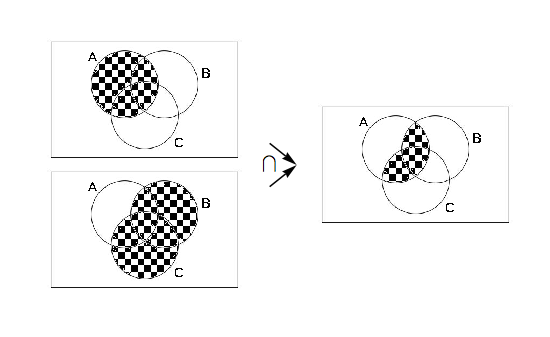
\includegraphics[width=\linewidth]{images/distrib-venn-lhs.png}
\end{image}%
\tcblower
\end{figureptx}%
\begin{figureptx}{Development of the right side of the distributive law for sets}{x:figure:distrib-venn-rhs}{}%
\begin{image}{0}{1}{0}%
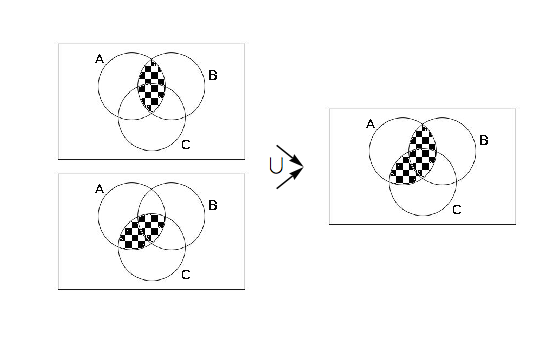
\includegraphics[width=\linewidth]{images/distrib-venn-rhs.png}
\end{image}%
\tcblower
\end{figureptx}%
\end{subsectionptx}
%
%
\typeout{************************************************}
\typeout{Subsection 4.1.3 Proof using Set-membership Tables}
\typeout{************************************************}
%
\begin{subsectionptx}{Proof using Set-membership Tables}{}{Proof using Set-membership Tables}{}{}{x:subsection:ss-membership-table-proof}
Let \(A\) be a subset of a universal set \(U\) and let \(u\in U\). To use this method we note that exactly one of the following is true: \(u \in  A\) or \(u\notin  A\). Denote the situation where \(u \in  A\) by 1 and that where \(u \notin  A\) by 0. Working with two sets, \(A\) and \(B\), and if \(u \in  U\), there are four possible outcomes of ``where \(u\) can be.'' What are they? The set-membership table for \(A \cup  B\) is:%
\begin{tableptx}{\textbf{Membership Table for \(A \cup  B\)}}{x:table:mt-union}{}%
\centering
{\tabularfont%
\begin{tabular}{ccc}
\(A\)&\(B\)&\(A \cup  B\)\tabularnewline[0pt]
0&0&0\tabularnewline[0pt]
0&1&1\tabularnewline[0pt]
1&0&1\tabularnewline[0pt]
1&1&1
\end{tabular}
}%
\end{tableptx}%
This table illustrates that \(u\in A \cup  B\) if and only if \(u\in A\) or \(u \in  B\).%
\par
In order to prove the distributive law via a set-membership table, write out the table for each side of the set statement to be proved and note that if \(S\) and \(T\) are two columns in a table, then the set statement \(S\) is equal to the set statement \(T\) if and only if corresponding entries in each row are the same.%
\par
To prove \(A \cap  (B \cup  C) = (A \cap  B) \cup  (A \cap  C)\), first note that the statement involves three sets, \(A\), \(B\), and \(C\), so there are \(2^3= 8\) possibilities for the membership of an element in the sets.%
\begin{tableptx}{\textbf{Membership table to prove the distributive law of intersection over union}}{x:table:tab-mt-distr}{}%
\centering
{\tabularfont%
\begin{tabular}{cccccccc}
\(A\)&\(B\)&\(C\)&\(B \cup  C\)&\(A \cap B\)&\(A \cap C\)&\(A \cap  (B \cup  C)\)&\((A \cap  B) \cup  (A \cap  C)\)\tabularnewline[0pt]
0&0&0&0&0&0&0&0\tabularnewline[0pt]
0&0&1&1&0&0&0&0\tabularnewline[0pt]
0&1&0&1&0&0&0&0\tabularnewline[0pt]
0&1&1&1&0&0&0&0\tabularnewline[0pt]
1&0&0&0&0&0&0&0\tabularnewline[0pt]
1&0&1&1&0&1&1&1\tabularnewline[0pt]
1&1&0&1&1&0&1&1\tabularnewline[0pt]
1&1&1&1&1&1&1&1
\end{tabular}
}%
\end{tableptx}%
Since each entry in Column 7 is the same as the corresponding entry in Column 8, we have shown that \(A\cap  (B \cup  C) = (A\cap B) \cup  (A \cap C)\) for any sets \(A\), \(B\), and \(C\). The main advantage of this method is that it is mechanical. The main disadvantage is that it is reasonable to use only for a relatively small number of sets. If we are trying to prove a statement involving five sets, there are \(2^5 = 32\) rows, which would test anyone's patience doing the work by hand.%
\end{subsectionptx}
%
%
\typeout{************************************************}
\typeout{Subsection 4.1.4 Proof Using Definitions}
\typeout{************************************************}
%
\begin{subsectionptx}{Proof Using Definitions}{}{Proof Using Definitions}{}{}{x:subsection:ss-proofs-using-definitions-sets}
This method involves using definitions and basic concepts to prove the given statement. This procedure forces one to learn, relearn, and understand basic definitions and concepts. It helps individuals to focus their attention on the main ideas of each topic and therefore is the most useful method of proof. One does not learn a topic by memorizing or occasionally glancing at core topics, but by using them in a variety of contexts. The word proof panics most people; however, everyone can become comfortable with proofs. Do not expect to prove every statement immediately. In fact, it is not our purpose to prove every theorem or fact encountered, only those that illustrate methods and\slash{}or basic concepts. Throughout the text we will focus in on main techniques of proofs. Let's illustrate by proving the distributive law.%
\par
\emph{Proof Technique 1.}  State or restate the theorem so you understand what is given (the hypothesis) and what you are trying to prove (the conclusion).%
\begin{theorem}{The Distributive Law of Intersection over Union.}{}{x:theorem:th-distr-law-i-over-u}%
If \(A\), \(B\), and \(C\) are sets, then \(A\cap  (B \cup  C) = (A\cap B) \cup  (A \cap  C)\).%
\end{theorem}
\begin{proof}{}{g:proof:idm40460654704}
What we can assume: \(A\), \(B\), and \(C\) are sets.%
\par
What we are to prove: \(A\cap  (B \cup  C) = (A\cap B) \cup  (A \cap  C)\).%
\par
Commentary: What types of objects am I working with: sets? real numbers? propositions? The answer is sets: sets of elements that can be anything you care to imagine. The universe from which we draw our elements plays no part in the proof of this theorem.%
\par
We need to show that the two sets are equal. Let's call them the left-hand set \((LHS\)) and the right-hand set (\(RHS\)). To prove that \(LHS = RHS\), we must prove two things: (a) \(LHS\subseteq RHS\), and (b) \(RHS \subseteq LHS\).%
\par
To prove part a and, similarly, part b, we must show that each element of \(LHS\) is an element of \(RHS\).  Once we have diagnosed the problem we are ready to begin.%
\par
We must prove: (a) \(A \cap  (B \cup  C)\subseteq (A\cap B) \cup  (A\cap C)\).%
\par
Let \(x \in  A\cap (B \cup  C)\):%
\begin{equation*}
\begin{split}
x \in A \cap (B \cup C) & \Rightarrow x\in A \textrm{ and } (x\in B\textrm{ or } x\in C)\\
& \quad \textrm{def. of union and intersection}\\
& \Rightarrow  (x \in A\textrm{ and }x\in B)\textrm{ or } (x\in A\textrm{ and }x\in C)\\
&\quad \textrm{distributive law of logic}\\
& \Rightarrow  (x \in A \cap B) \textrm{ or } (x \in A \cap C)\\
&\quad \textrm{def. of intersection}\\
& \Rightarrow  x \in (A \cap B) \cup (A \cap C)\\
&\quad \textrm{def. of union}
\end{split}
\end{equation*}
We must also prove (b) \((A\cap B) \cup  (A\cap C)\subseteq A \cap  (B \cup  C)\).%
\par
%
\begin{equation*}
\begin{split}
x\in (A\cap B) \cup  (A \cap C)& \Rightarrow  (x\in A\cap B)\text{or } (x\in A\cap C)\\
&\quad \textrm{ Why? } \\
& \Rightarrow (x\in A\textrm{ and }x\in B)\textrm{ or } (x\in A\textrm{ and }x\in C)\\
&\quad\textrm{ Why? }\\
&\Rightarrow  x\in A \textrm{ and } (x\in B\textrm{ or }x\in C)\\
&\quad\textrm{ Why? }\\
&\Rightarrow x\in A\cap (B\cup C)\\
&\quad\textrm{ Why? } \square
\end{split}\text{.}\qedhere
\end{equation*}
%
\end{proof}
\emph{Proof Technique 2}%
\par
%
\begin{enumerate}[label=(\arabic*)]
\item{}To prove that \(A\subseteq B\), we must show that if \(x \in  A\), then \(x \in  B\).%
\item{}To prove that \(A = B\), we must show:%
\par
%
\begin{enumerate}[label=(\alph*)]
\item{}\(A\subseteq B\) and%
\item{}\(B \subseteq A\).%
\end{enumerate}
%
\end{enumerate}
%
\par
To further illustrate the Proof-by-Definition technique, let's prove the following theorem.%
\begin{theorem}{Another Proof using Definitions.}{}{x:theorem:th-set-proof-example2}%
If  \(A\), \(B\), and \(C\) are any sets, then \(A \times  (B \cap  C) = (A \times  B) \cap  (A \times  C)\).%
\end{theorem}
\begin{proof}{}{g:proof:idm40460635200}
Commentary; We again ask ourselves: What are we trying to prove? What types of objects are we dealing with? We realize that we wish to prove two facts: (a) \(LHS\subseteq RHS\), and (b) \(RHS\subseteq LHS\).%
\par
To prove part (a), and similarly part (b), we'll begin the same way. Let  \(\_\_\_ \in  LHS\) to show \(\_\_\_ \in  RHS\). What should \(\_\_\_\) be?  What does a typical object in the \(LHS\) look like?%
\par
Now, on to the actual proof.%
\par
(a) \(A\times (B\cap  C)\subseteq (A\times B)\cap (A\times C)\).%
\par
Let \((x, y) \in  A\times (B\cap C)\).%
\begin{equation*}
\begin{split}
(x, y) \in A\times (B\cap C) &\Rightarrow x \in  A \textrm{ and } y \in  (B\cap  C)\\
&\quad \textrm{ Why? }\\
&\Rightarrow x \in  A \textrm{ and }(y \in  B\textrm{ and } y \in  C)\\
&\textrm{ Why? }\\
&\Rightarrow (x \in  A \textrm{ and } y \in  B) \textrm{ and } (x \in  A \textrm{ and } y \in C)\\
&\quad \textrm{ Why? }\\
&\Rightarrow  (x, y) \in  (A\times B) \textrm{ and } (x, y) \in  (A \times C)\\
&\quad \textrm{ Why? }\\
&\Rightarrow (x, y) \in  (A\times  B) \cap (A\times C)\\
&\quad \textrm{ Why? }
\end{split}
\end{equation*}
%
\par
(b) \((A\times  B)\cap (A\times C)\subseteq A\times ( B\cap C)\).%
\par
Let \((x, y) \in  (A\times  B) \cap  (A\times C)\).%
\begin{equation*}
\begin{split}
(x, y) \in  (A\times  B)\cap (A\times C) &\Rightarrow (x, y) \in  A\times  B\textrm{ and } (x, y) \in  A\times C\\
&\quad \textrm{ Why? }\\
&\Rightarrow (x \in  A \textrm{ and } y \in  B) \textrm{ and } (x \in  A \textrm{ and } y \in  C)\\
&\quad \textrm{ Why? }\\
&\Rightarrow  x \in  A \textrm{ and } (y \in  B\textrm{ and } y \in  C)\\
&\quad \textrm{ Why? }\\
&\Rightarrow  x \in  A\textrm{ and } y \in  (B\cap  C)\\
&\quad \textrm{ Why? }\\
&\Rightarrow (x, y) \in  A \times (B\cap  C)\\
&\quad \textrm{ Why? } 
\end{split}\qedhere
\end{equation*}
%
\end{proof}
\end{subsectionptx}
%
%
\typeout{************************************************}
\typeout{Exercises 4.1.5 Exercises}
\typeout{************************************************}
%
\begin{exercises-subsection}{Exercises}{}{Exercises}{}{}{g:exercises:idm40460626576}
\begin{divisionexercise}{1}{}{}{x:exercise:exercise-4-1-1}%
Prove the following:%
\begin{enumerate}[label=(\alph*)]
\item{}Let \(A\), \(B\), and \(C\) be sets. If \(A\subseteq B\) and \(B\subseteq C\), then \(A\subseteq C\).%
\item{}Let \(A\) and \(B\) be sets. Then \(A - B= A\cap B^c\) .%
\item{}Let \(A,B, \textrm{ and } C\) be sets. If (\(A\subseteq B\) and \(A\subseteq C\)) then \(A\subseteq B\cap C\).%
\item{}Let \(A \textrm{ and } B\) be sets. \(A\subseteq B\) if and only if \(B^c\subseteq A^c\) .%
\item{}Let \(A,B, \textrm{ and } C\) be sets. If \(A\subseteq B\) then \(A\times C \subseteq B\times C\).%
\end{enumerate}
%
\end{divisionexercise}%
\begin{divisionexercise}{2}{}{}{g:exercise:idm40460601696}%
Write the converse of parts (a), (c), and (e) of Exercise 1 and prove or disprove them.%
\end{divisionexercise}%
\begin{divisionexercise}{3}{}{}{g:exercise:idm40460596688}%
Disprove the following, assuming \(A, B, \textrm{ and } C\) are sets:%
\begin{enumerate}[label=(\alph*)]
\item{}\(A - B = B - A\).%
\item{}\(A\times B = B\times A\).%
\item{}\(A \cap   B = A  \cap   C\) implies \(B = C\).%
\item{}\(A \oplus  (B\cap C) = (A \oplus  B)\cap  (A \oplus C)\)%
\end{enumerate}
%
\end{divisionexercise}%
\begin{divisionexercise}{4}{}{}{g:exercise:idm40460584480}%
Let \(A, B, \textrm{ and } C\) be sets. Write the following in ``if . . . then . . .'' language and prove:%
\begin{enumerate}[label=(\alph*)]
\item{}\(x \in  B\) is a sufficient condition for \(x \in  A \cup B\).%
\item{}\(A \cap B\cap C = \emptyset\) is a necessary condition for \(A \cap  B =\emptyset\).%
\item{}\(A \cup  B = B\) is a necessary and sufficient condition for \(A\subseteq  B\).%
\end{enumerate}
%
\end{divisionexercise}%
\begin{divisionexercise}{5}{}{}{x:exercise:ex-generalized_distrib}%
Prove by induction that if \(A\), \(B_1\), \(B_2\), ... , \(B_n\) are sets, \(n\geq 2\), then \(A\cap ( B_1 \cup  B_2\cup  \dots  \cup  B_n) = (A \cap B_1) \cup  (A \cap B_2 ) \cup  \dots \cup  (A\cap B_n)\).%
\end{divisionexercise}%
\begin{divisionexercise}{6}{}{}{x:exercise:exercise-disjoint-not-transitive}%
Let \(A\), \(B\) and \(C\) be sets. Prove or disprove:%
\begin{equation*}
A \cap B \neq \emptyset,  B \cap C \neq \emptyset \Rightarrow A\cap C \neq \emptyset
\end{equation*}
%
\end{divisionexercise}%
\end{exercises-subsection}
\end{sectionptx}
%
%
\typeout{************************************************}
\typeout{Section 4.2 Laws of Set Theory}
\typeout{************************************************}
%
\begin{sectionptx}{Laws of Set Theory}{}{Laws of Set Theory}{}{}{x:section:s-laws-of-set-theory}
%
%
\typeout{************************************************}
\typeout{Subsection 4.2.1 Tables of Laws}
\typeout{************************************************}
%
\begin{subsectionptx}{Tables of Laws}{}{Tables of Laws}{}{}{g:subsection:idm40460562864}
The following basic set laws can be derived using either the Basic Definition or the Set-Membership approach and can be illustrated by Venn diagrams.%
\begin{tableptx}{\textbf{Basic Laws of Set Theory}}{x:table:table-set-laws}{}%
\centering
{\tabularfont%
\begin{tabular}{ccc}
&&\tabularnewline[0pt]
&Commutative Laws&\tabularnewline[0pt]
(1) \(A \cup B = B \cup  A\)&&(\(1^{\prime}\)) \(A \cap B = B\cap A\)\tabularnewline\hrulethin
&Associative Laws&\tabularnewline[0pt]
(2) \(A \cup  (B \cup  C)= (A\cup B)\cup C\)&&(\(2^{\prime}\)) \(A \cap  (B \cap  C) = (A \cap  B) \cap  C \)\tabularnewline\hrulethin
&Distributive Laws&\tabularnewline[0pt]
(3) \(A\cap (B \cup  C)=(A\cap B )\cup (A\cap  C)\)&&(\(3^{\prime}\)) \(A \cup (B \cap C) = (A \cup B ) \cap (A\cup C)\)\tabularnewline\hrulethin
&Identity Laws&\tabularnewline[0pt]
(4) \(A \cup  \emptyset  = \emptyset  \cup  A = A\)&&(\(4^{\prime}\)) \(A \cap  U = U \cap  A = A\)\tabularnewline\hrulethin
&Complement Laws&\tabularnewline[0pt]
(5) \(A\cup A^c= U\)&&(\(5^{\prime}\)) \(A\cap A^c= \emptyset\)\tabularnewline\hrulethin
&Idempotent Laws&\tabularnewline[0pt]
(6) \(A \cup  A = A\)&&(\(6^{\prime}\)) \(A\cap  A = A\)\tabularnewline\hrulethin
&Null Laws&\tabularnewline[0pt]
(7) \(A \cup  U = U\)&&(\(7^{\prime}\)) \(A \cap  \emptyset  =\emptyset\)\tabularnewline\hrulethin
&Absorption Laws&\tabularnewline[0pt]
(8) \(A \cup  (A\cap  B) = A\)&&(\(8^{\prime}\)) \(A\cap (A \cup  B) = A\)\tabularnewline\hrulethin
&DeMorgan's Laws&\tabularnewline[0pt]
(9) \((A \cup  B)^c= A^c\cap  B^c\)&&(\(9^{\prime}\)) \((A\cap  B)^c = A^c \cup  B^c\)\tabularnewline\hrulethin
&Involution Law&\tabularnewline[0pt]
&(10) \((A^c)^c= A\)&\tabularnewline\hrulethin
\end{tabular}
}%
\end{tableptx}%
It is quite clear that most of these laws resemble or, in fact, are analogues of laws in basic algebra and the algebra of propositions.%
\end{subsectionptx}
%
%
\typeout{************************************************}
\typeout{Subsection 4.2.2 Proof Using Previously Proven Theorems}
\typeout{************************************************}
%
\begin{subsectionptx}{Proof Using Previously Proven Theorems}{}{Proof Using Previously Proven Theorems}{}{}{x:subsection:ss-proof-with-theorems}
Once a few basic laws or theorems have been established, we frequently use them to prove additional theorems. This method of proof is usually more efficient than that of proof by Definition. To illustrate, let us prove the following Corollary to the Distributive Law.   The term "corollary" is used for theorems that can be proven with relative ease from previously proven theorems.%
\begin{corollary}{A Corollary to the Distributive Law of Sets.}{}{x:corollary:th-corollary-to-distr}%
Let A and B be sets. Then \((A\cap  B) \cup  (A\cap  B^c) = A\).%
\end{corollary}
\begin{proof}{}{g:proof:idm40460529680}
%
\begin{equation*}
\begin{split}
(A\cap  B) \cup  (A\cap  B^c) & = A \cap (B \cup B^c)\\
& \quad \textrm{Why?}\\
& = A \cap U\\ 
&\quad  \textrm{Why?}\\
& = A\\
&\quad \textrm{Why?} 
\end{split}\text{.}\qedhere
\end{equation*}
%
\end{proof}
\end{subsectionptx}
%
%
\typeout{************************************************}
\typeout{Subsection 4.2.3 Proof Using the Indirect Method\slash{}Contradiction}
\typeout{************************************************}
%
\begin{subsectionptx}{Proof Using the Indirect Method\slash{}Contradiction}{}{Proof Using the Indirect Method\slash{}Contradiction}{}{}{x:subsection:ss-proof-sets-contradiction}
The procedure one most frequently uses to prove a theorem in mathematics is the Direct Method, as illustrated in \hyperref[x:theorem:th-distr-law-i-over-u]{Theorem~{\xreffont\ref{x:theorem:th-distr-law-i-over-u}}} and \hyperref[x:theorem:th-set-proof-example2]{Theorem~{\xreffont\ref{x:theorem:th-set-proof-example2}}}. Occasionally there are situations where this method is not applicable. Consider the following:%
\begin{theorem}{An Indirect Proof in Set Theory.}{}{x:theorem:theorem-example-sets-contradiction}%
Let \(A, B, C\) be sets. If \(A\subseteq B\) and \(B\cap C = \emptyset\), then \(A\cap C = \emptyset\).%
\end{theorem}
\begin{proof}{}{g:proof:idm40460522944}
Commentary: The usual and first approach would be to assume \(A\subseteq B\) and \(B\cap C = \emptyset\) is true and to attempt to prove \(A\cap C = \emptyset\) is true. To do this you would need to show that nothing is contained in the set \(A \cap  C\). Think about how you would show that something doesn't exist. It is very difficult to do directly.%
\par
The Indirect Method is much easier: If we assume the conclusion is false and we obtain a contradiction -{}-{}-  then the theorem must be true. This approach is on sound logical footing since it is exactly the same method of indirect proof that we discussed in \hyperref[x:subsection:sub-indirect-proof]{Subsection~{\xreffont\ref{x:subsection:sub-indirect-proof}}}.%
\par
Assume \(A\subseteq B\) and \(B\cap C = \emptyset\), and \(A\cap C \neq  \emptyset\). To prove that this cannot occur, let \(x\in A \cap C\).%
\par
%
\begin{equation*}
\begin{split}
x \in A \cap C & \Rightarrow x \in A \textrm{ and } x \in  C\\
& \Rightarrow x \in B \textrm{ and } x \in  C\\
& \Rightarrow x \in  B \cap C
\end{split}\text{.}
\end{equation*}
%
\par
But this contradicts the second premise.  Hence, the theorem is proven.%
\end{proof}
\end{subsectionptx}
%
%
\typeout{************************************************}
\typeout{Exercises 4.2.4 Exercises}
\typeout{************************************************}
%
\begin{exercises-subsection}{Exercises}{}{Exercises}{}{}{x:exercises:exer-4-2}
\begin{introduction}{}%
In the exercises that follow it is most important that you outline the logical procedures or methods you use.%
\end{introduction}%
\begin{divisionexercise}{1}{}{}{g:exercise:idm40460515184}%
%
\begin{enumerate}[label=(\alph*)]
\item{}Prove the associative law for intersection (Law \(2^{\prime}\)) with a Venn diagram.%
\item{}Prove DeMorgan's Law (Law 9) with a membership table.%
\item{}Prove the Idempotent Law (Law 6) using basic definitions.%
\end{enumerate}
%
\end{divisionexercise}%
\begin{divisionexercise}{2}{}{}{g:exercise:idm40460507232}%
%
\begin{enumerate}[label=(\alph*)]
\item{}Prove the Absorption Law (Law \(8^{\prime}\)) with a Venn diagram.%
\item{}Prove the Identity Law (Law 4) with a membership table.%
\item{}Prove the Involution Law (Law 10) using basic definitions.%
\end{enumerate}
%
\end{divisionexercise}%
\begin{divisionexercise}{3}{}{}{g:exercise:idm40460505120}%
Prove the following using the set theory laws, as well as any other theorems proved so far.%
\par
%
\begin{enumerate}[label=(\alph*)]
\item{}\(\displaystyle A \cup  (B - A) = A \cup  B\)%
\item{}\(\displaystyle A - B = B^c - A ^c\)%
\item{}\(\displaystyle A\subseteq B, A\cap C \neq \emptyset  \Rightarrow  B\cap C \neq \emptyset\)%
\item{}\(\displaystyle A\cap (B - C) = (A\cap B) - (A\cap C)\)%
\item{}\(\displaystyle A - (B \cup  C) = (A - B)\cap (A - C)\)%
\end{enumerate}
%
\end{divisionexercise}%
\begin{divisionexercise}{4}{}{}{g:exercise:idm40460494096}%
Use previously proven theorems to prove the following.%
\par
%
\begin{enumerate}[label=(\alph*)]
\item{}\(\displaystyle A \cap (B\cap C)^c= (A\cap B^c)\cup (A\cap C^{c })\)%
\item{}\(\displaystyle A \cap (B\cap (A\cap B)^c)= \emptyset\)%
\item{}\(\displaystyle (A\cap B) \cup  B^c = A \cup  B^c\)%
\item{}\(A \cup  (B - C) = (A \cup  B) - (C - A)\).%
\end{enumerate}
%
\end{divisionexercise}%
\begin{divisionexercise}{5}{Hierarchy of Set Operations.}{}{g:exercise:idm40460490464}%
The rules that determine the order of evaluation in a set expression that involves more than one operation are similar to the rules for logic. In the absence of parentheses, complementations are done first, intersections second, and unions third. Parentheses are used to override this order. If the same operation appears two or more consecutive times, evaluate from left to right. In what order are the following expressions performed?%
\par
%
\begin{multicols}{2}
\begin{enumerate}[label=(\alph*)]
\item{}\(A \cup  B^c\cap C\).%
\item{}\(A\cap B \cup  C\cap B\).%
\item{}\(\displaystyle A \cup  B \cup  C^c\)%
\end{enumerate}
\end{multicols}
%
\end{divisionexercise}%
\begin{divisionexercise}{6}{}{}{g:exercise:idm40460483200}%
There are several ways that we can use to format the proofs in this chapter. One that should be familiar to you from Chapter 3 is illustrated with the following alternate proof of part (a) in \hyperref[x:theorem:th-distr-law-i-over-u]{Theorem~{\xreffont\ref{x:theorem:th-distr-law-i-over-u}}}:%
\begin{tableptx}{\textbf{An alternate format for the proof of Theorem~{\xreffont\ref*{x:theorem:th-distr-law-i-over-u}}}}{x:table:tt-conditional-proof}{}%
\centering
{\tabularfont%
\begin{tabular}{ccc}
(1)&\(x \in  A \cap  (B \cup  C)\)&Premise\tabularnewline[0pt]
(2)&\((x \in  A) \land  (x \in  B \cup  C)\)&(1), definition of intersection\tabularnewline[0pt]
(3)&(\(x \in  A) \land ((x \in  B) \lor  (x \in  C))\)&(2), definition of union\tabularnewline[0pt]
(4)&\((x \in A)\land (x\in  B)\lor  (x \in A)\land (x\in  C)\)&(3), distribute \(\land\) over \(\lor\)\tabularnewline[0pt]
(5)&\((x \in  A\cap B) \lor (x \in  A \cap C)\)&(4), definition of intersection\tabularnewline[0pt]
(6)&\(x \in  (A \cap B) \cup  (A \cap C)\)&(5), definition of union \(\blacksquare\)
\end{tabular}
}%
\end{tableptx}%
Prove part (b) of \hyperref[x:theorem:th-set-proof-example2]{Theorem~{\xreffont\ref{x:theorem:th-set-proof-example2}}} and \hyperref[x:theorem:theorem-example-sets-contradiction]{Theorem~{\xreffont\ref{x:theorem:theorem-example-sets-contradiction}}} using this format.%
\end{divisionexercise}%
\end{exercises-subsection}
\end{sectionptx}
%
%
\typeout{************************************************}
\typeout{Section 4.3 Minsets}
\typeout{************************************************}
%
\begin{sectionptx}{Minsets}{}{Minsets}{}{}{x:section:s-minsets}
%
%
\typeout{************************************************}
\typeout{Subsection 4.3.1 Definition of Minsets}
\typeout{************************************************}
%
\begin{subsectionptx}{Definition of Minsets}{}{Definition of Minsets}{}{}{g:subsection:idm40460468080}
Let \(B_1\) and \(B_2\) be subsets of a set \(A\). Notice that the Venn diagram of \hyperref[x:figure:fig-minsets-2]{Figure~{\xreffont\ref{x:figure:fig-minsets-2}}} is naturally partitioned into the subsets \(A_1\), \(A_2\), \(A_3\), and \(A_4\). Further we observe that \(A_1\), \(A_2\), \(A_3\), and \(A_4\) can be described in terms of \(B_1\) and \(B_2\) as follows:%
\begin{figureptx}{Venn Diagram of Minsets}{x:figure:fig-minsets-2}{}%
\begin{image}{0.165}{0.67}{0.165}%
\IfFileExists{images/minsets-2.pdf}%
{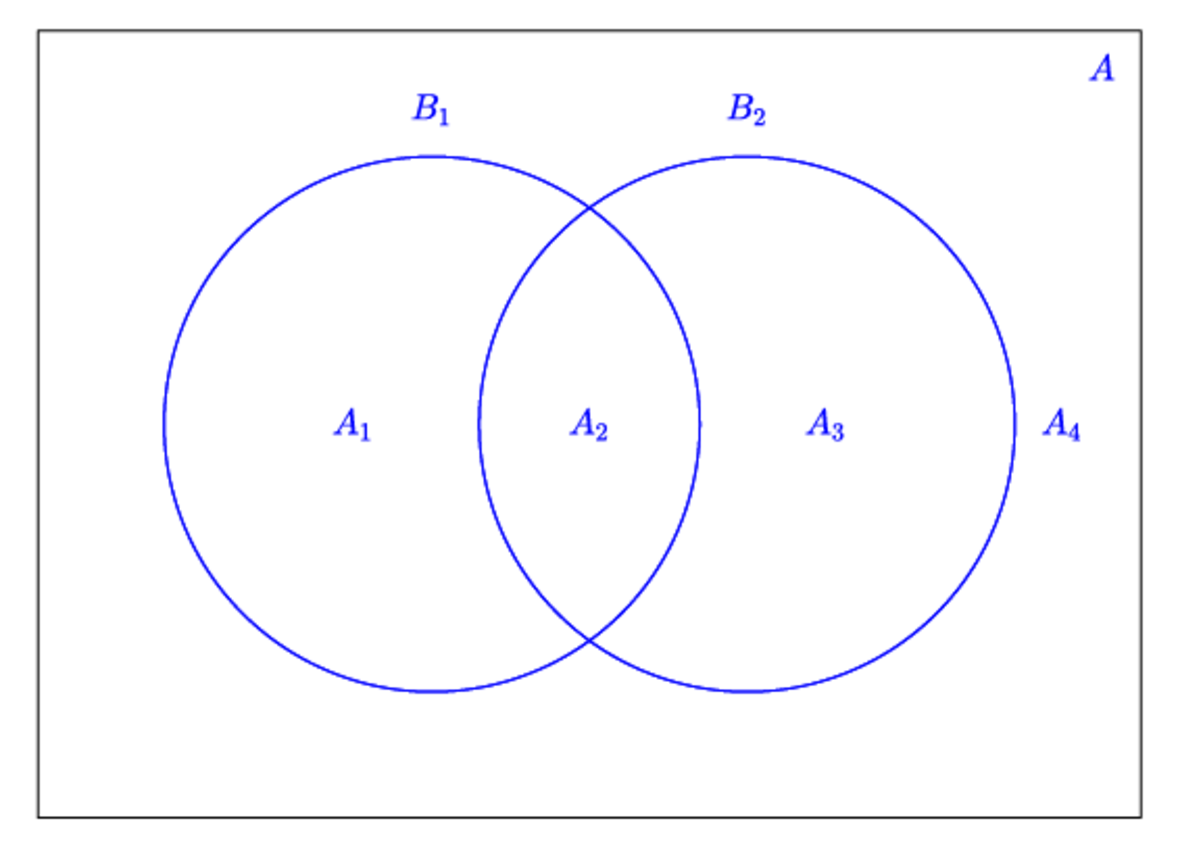
\includegraphics[width=\linewidth]{images/minsets-2.pdf}}%
{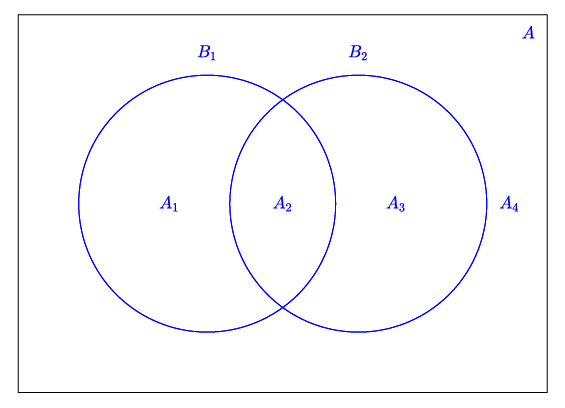
\includegraphics[width=\linewidth]{images/minsets-2.png}}
\end{image}%
\tcblower
\end{figureptx}%
\begin{tableptx}{\textbf{Minsets generated by two sets}}{x:table:tab-minsets-2}{}%
\centering
{\tabularfont%
\begin{tabular}{c}
\(A_1=B_1\cap B_2^c\)\tabularnewline[0pt]
\(A_2=B_1\cap B_2\)\tabularnewline[0pt]
\(A_3= B_1^c\cap B_2\)\tabularnewline[0pt]
\(A_4= B_1^c\cap B_2^c\)
\end{tabular}
}%
\end{tableptx}%
Each \(A_i\) is called a minset generated by \(B_1\) and \(B_2\). We note that each minset is formed by taking the intersection of two sets where each may be either \(B_k\) or its complement, \(B_k^c\). Note also, given two sets, there are \(2^{2}=4\) minsets.%
\par
Minsets are occasionally called \emph{minterms}.%
\par
The reader should note that if we apply all possible combinations of the operations intersection, union, and complementation to the sets \(B_1\) and \(B_2\) of \hyperref[x:figure:fig-minsets-2]{Figure~1}, the smallest sets generated will be exactly the minsets, the minimum sets. Hence the derivation of the term minset.%
\par
Next, consider the Venn diagram containing three sets, \(B_1\), \(B_2\), and \(B_3\). Draw it right now and count the regions! What are the minsets generated by \(B_1\), \(B_2\), and \(B_3\)? How many are there? Following the procedures outlined above, we note that the following are three of the \(2^3=8\) minsets. What are the others?%
\begin{tableptx}{\textbf{Three of the minsets generated by \(B_1\), \(B_2\), and \(B_3\)}}{x:table:tab-some-minsets-3}{}%
\centering
{\tabularfont%
\begin{tabular}{c}
\(B_1\cap B_2\cap B_3^c\)\tabularnewline[0pt]
\(B_1\cap B_2^c\cap B_3\)\tabularnewline[0pt]
\(B_1\cap B_2^c\cap B_3^c\)
\end{tabular}
}%
\end{tableptx}%
\begin{definition}{Minset.}{x:definition:def-Minset}%
\index{Minset}%
Let \(\{B_1, B_2,\ldots,B_n\}\) be a set of subsets of  set \(A\). Sets of the form \(D_1\cap D_2\cap
\cdots \cap D_n\), where each \(D_i\) may be either \(B_i\) or \(B_i^c\), is called a minset generated by \(B_1\), \(B_2\),... and  \(B_n\).%
\end{definition}
\begin{example}{A concrete example of some minsets.}{x:example:ex-minset-example}%
Consider the following concrete example. Let \(A = \{1, 2, 3, 4, 5, 6\}\) with subsets \(B_1 = \{1,3,5\}\) and \(B_2= \{1,2,3\}\). How can we use set operations applied to and produce a partition of \(A\)? As a first attempt, we might try these three sets:%
\begin{tableptx}{\textbf{}}{x:table:tab-subsets-generated-1}{}%
\centering
{\tabularfont%
\begin{tabular}{c}
\(B_1\cap B_2=\{1,3\}\)\tabularnewline[0pt]
\(B_1^c=\{2,4,6\}\)\tabularnewline[0pt]
\(B_2^c=\{4,5,6\}\).
\end{tabular}
}%
\end{tableptx}%
We have produced all elements of \(A\) but we have 4 and 6 repeated in two sets. In place of \(B_1^c\) and \(B_2^c\), let's try \(B_1^c\cap B_2\) and \(B_1\cap B_2^c\), respectively:%
\begin{tableptx}{\textbf{}}{x:table:tab-subsets-generated-2}{}%
\centering
{\tabularfont%
\begin{tabular}{c}
\(B_1^c\cap B_2=\{2\}\) and\tabularnewline[0pt]
\(B_1\cap B_2^c=\{5\}\).
\end{tabular}
}%
\end{tableptx}%
We have now produced the elements 1, 2, 3, and 5 using \(B_1\cap B_2\),  \(B_1^c\cap B_2\) and \(B_1\cap B_2^c\) yet we have not listed the elements 4 and 6. Most ways that we could combine \(B_1\) and \(B_2\) such as \(B_1\cup B_2\) or \(B_1\cup B_2^c\) will produce duplications of listed elements and will not produce both 4 and 6. However we note that \(B_1^c\cap B_2^c= \{4, 6\}\), exactly the elements we need.%
\par
After more experimenting, we might reach a conclusion that each element of \(A\) appears exactly once in one of the four minsets \(B_1\cap B_2\) ,  \(B_1^c\cap B_2\), \(B_1\cap B_2^c\) and \(B_1^c\cap B_2^c\). Hence, we have a partition of \(A\). In fact this is the finest partition of \(A\) in that all other partitions we could generate consist of selected unions of these minsets.%
\par
At this point, we might ask and be able to answer the question ``How many different subsets of our universe can we generate from  \(B_1\) and \(B_2\)?''  The answer is \(2^{\textrm{number of nonempty minsets}}\), which is \(2^4=16\) in this case.  Notice that in general, it would be impossible to find two sets from which we could generate all subsets of \(A=\{1, 2, 3, 4, 5, 6\}\) since there will never be more than four nonempty minsets.   If we allowed ourselves three subsets and tried to generat all sets from them, then the number of minsets would be \(2^3 =8\).  With only six elements in \(A\), there could be six minsets, each containing a single element.  In that case we could generate the whole power set of \(A\).%
\end{example}
\end{subsectionptx}
%
%
\typeout{************************************************}
\typeout{Subsection 4.3.2 Properties of Minsets}
\typeout{************************************************}
%
\begin{subsectionptx}{Properties of Minsets}{}{Properties of Minsets}{}{}{g:subsection:idm40460467952}
\begin{theorem}{Minset Partition Theorem.}{}{x:theorem:th-minset-partition}%
Let \(A\) be a set and let \(B_1\), \(B_2\) \(\ldots\)  , \(B_n\) be subsets of \(A\). The set of nonempty minsets generated by  \(B_1\), \(B_2\) \(\ldots\)  , \(B_n\) is a partition of \(A\).%
\end{theorem}
\begin{proof}{}{g:proof:idm40460412160}
The proof of this theorem is left to the reader.%
\end{proof}
One of the most significant facts about minsets is that any subset of \(A\) that can be obtained from  \(B_1\), \(B_2\) \(\ldots\), \(B_n\), using the standard set operations can be obtained in a standard form by taking the union of selected minsets.%
\begin{definition}{Minset Normal Form.}{x:definition:def-minset-normal-form}%
\index{Minset Normal Form}%
A set is said to be in minset normal form when it is expressed as the union of zero or more distinct nonempty minsets.%
\end{definition}
Notes:%
\par
%
\begin{itemize}[label=\textbullet]
\item{}The union of zero sets is the empty set, \(\emptyset\).%
\item{}Minset normal form is also called \terminology{canonical form}.%
\end{itemize}
%
\begin{example}{Another Concrete Example of Minsets.}{x:example:ex-concrete-minsets-2}%
Let \(U = \{-2,-1,0,1,2\}\), \(B_1= \{0,1,2\}\), and \(B_2= \{0,2\}\).  Then%
\begin{tableptx}{\textbf{}}{g:table:idm40460398208}{}%
\centering
{\tabularfont%
\begin{tabular}{c}
\(B_1\cap B_2=\{0,2\}\)\tabularnewline[0pt]
\(B_1^c\cap B_2 = \emptyset\)\tabularnewline[0pt]
\(B_1\cap B_2^c = \{1\}\)\tabularnewline[0pt]
\(B_1^c\cap B_2^c = \{-2,-1\}\)
\end{tabular}
}%
\end{tableptx}%
In this case, there are only three nonempty minsets, producing the partition \(\{\{0,2\},\{1\},\{-2,-1\}\}\). An example of a set that could not be produced from just \(B_1\) and \(B_2\) is the set of even elements of \(U\), \(\{-2,0,2\}\). This is because \(-2\) and \(-1\) cannot be separated. They are in the same minset and any union of minsets either includes or excludes them both.  In general, there are \(2^3= 8\) different minset normal forms because there are three nonempty minsets. This means that only 8 of the \(2^5=32\) subsets of \(U\) could be generated from  any two sets \(B_1\) and \(B_2\).%
\end{example}
\end{subsectionptx}
%
%
\typeout{************************************************}
\typeout{Exercises 4.3.3 Exercises}
\typeout{************************************************}
%
\begin{exercises-subsection}{Exercises}{}{Exercises}{}{}{x:exercises:exercises-4-3}
\begin{divisionexercise}{1}{}{}{g:exercise:idm40460388576}%
Consider the subsets \(A = \{1, 7, 8\}\), \(B = \{1, 6, 9, 10\}\), and \(C = \{1, 9, 10\}\), where \(U = \{1,2, . . . , 10\}\).%
\par
%
\begin{enumerate}[label=(\alph*)]
\item{}List the nonempty minsets generated by \(A, B, \textrm{ and } C\).%
\item{}How many elements of the power set of \(U\) can be generated by \(A\), \(B\), and \(C\)? Compare this number with \(\mid\mathcal{P}(U)\mid\).  Give an example of one subset that cannot be generated by \(A\), \(B\), and \(C\).%
\end{enumerate}
%
\end{divisionexercise}%
\begin{divisionexercise}{2}{}{}{g:exercise:idm40460377248}%
%
\begin{enumerate}[label=(\alph*)]
\item{}Partition \(\{1, 2, .... 9\}\) into the minsets generated by \(B_1= \{5, 6,7\}\), \(B_2 = \{2, 4, 5, 9\}\), and \(B_3 = \{3, 4, 5, 6, 8, 9\}\).%
\item{}How many different subsets of \(\{1, 2, . . . ,9\}\) can you create using \(B_1, B_2\), and \(B_3\) with the standard set operations?%
\item{}Do there exist subsets \(C_1, C_2, C_3\) whose minsets will generate every subset of \(\{1,2, . . . ,9\}\)?%
\end{enumerate}
%
\end{divisionexercise}%
\begin{divisionexercise}{3}{}{}{g:exercise:idm40460371040}%
Partition the set of strings of 0's and 1's of length two or less, using the minsets generated by \(B_1=\{s \mid s \textrm{ has length } 2\}\), and \(B_2= \{s \mid s \textrm{ starts with a }   0\}\).%
\end{divisionexercise}%
\begin{divisionexercise}{4}{}{}{x:exercise:exercise-minsets-3}%
Let \(B_1, B_2\), and \(B_3\) be subsets of a universal set \(U\),%
\par
%
\begin{enumerate}[label=(\alph*)]
\item{}Symbolically list all minsets generated by \(B_1, B_2\), and \(B_3\).%
\item{}Illustrate with a Venn diagram all minsets obtained in part (a).%
\item{}Express the following sets in minset normal form: \(B_1^c\), \(B_1\cap B_2\) , \(B_1\cup B_2^c\).%
\end{enumerate}
%
\end{divisionexercise}%
\begin{divisionexercise}{5}{}{}{g:exercise:idm40460360384}%
%
\begin{enumerate}[label=(\alph*)]
\item{}Partition \(A = \{0, 1, 2, 3, 4, 5\}\) with the minsets generated by \(B_1= \{0, 2, 4\}\text{  }\)and \(B_2= \{1, 5\}\).%
\item{}How many different subsets of \(A\) can you generate from  \(B_1 \textrm{ and } B_2\)?%
\end{enumerate}
%
\end{divisionexercise}%
\begin{divisionexercise}{6}{}{}{g:exercise:idm40460352928}%
If \(\left\{B_1, B_2, \ldots , B_n\right\}\) is a partition of \(A\), how many minsets are generated by \(B_1, B_2, \ldots , B_n\)?%
\end{divisionexercise}%
\begin{divisionexercise}{7}{}{}{g:exercise:idm40460351040}%
Prove \hyperref[x:theorem:th-minset-partition]{Theorem~{\xreffont\ref{x:theorem:th-minset-partition}}}%
\end{divisionexercise}%
\begin{divisionexercise}{8}{}{}{g:exercise:idm40460349392}%
Let \(S\) be a finite set of \(n\) elements. Let \(B_i\), \(i = 1, 2, \ldots , k\) be nonempty subsets of \(S\). There are \(2^{2^k}\) minset normal forms generated by the \(k\) subsets. The number of subsets of \(S\) is \(2^n\). Since we can make \(2^{2^k} > 2^n\) by choosing \(k \geq  \log _2 n\), it is clear that two distinct minset normal-form expressions do not always equal distinct subsets of \(S\). Even for \(k < \log _2 n\), it may happen that two distinct minset normal-form expressions equal the same subset of \(S\). Determine necessary and sufficient conditions for distinct normal-form expressions to equal distinct subsets of \(S\).%
\end{divisionexercise}%
\end{exercises-subsection}
\end{sectionptx}
%
%
\typeout{************************************************}
\typeout{Section 4.4 The Duality Principle}
\typeout{************************************************}
%
\begin{sectionptx}{The Duality Principle}{}{The Duality Principle}{}{}{x:section:s-duality-principle}
%
%
\typeout{************************************************}
\typeout{Subsection 4.4.1 }
\typeout{************************************************}
%
\begin{subsectionptx}{}{}{}{}{}{g:subsection:idm40460331440}
In Section 4.2, we observed that each of the \hyperref[x:table:table-set-laws]{Table~{\xreffont\ref{x:table:table-set-laws}}} labeled 1 through 9 had an analogue \(1^{\prime}\) through \(9^{\prime}\). We notice that each of the laws in one column can be obtained from the corresponding law in the other column by replacing \(\cup\) by \(\cap \), \(\cap \) by \(\cup \), \(\emptyset \) by \(U\), \(U\) by \(\emptyset\), and leaving the complement unchanged.%
\begin{definition}{Duality Principle for Sets.}{x:definition:def-duality-sets}%
Let \(S\) be any identity involving sets and the operations complement, intersection and union. If \(S*\) is obtained from \(S\) by making the substitutions \(\cup  \to  \cap\), \(\cap \to \cup\), \(\emptyset \to U\) , and \(U\to \emptyset\), then the statement \(S*\) is also true and it is called the dual of the statement \(S\).%
\end{definition}
\begin{example}{Example of a dual.}{x:example:ex-dual-example}%
The dual of \((A \cap  B) \cup  \left(A \cap B^c \right) = A\) is \((A\cup B)\cap \left(A\cup B^c\right)=A\).%
\end{example}
One should not underestimate the importance of this concept. It gives us a whole second set of identities, theorems, and concepts. For example, we can consider the dual of \emph{minsets} and \emph{minset normal form} to obtain what is called \emph{maxsets} and \emph{maxset normal form}.%
\end{subsectionptx}
%
%
\typeout{************************************************}
\typeout{Exercises 4.4.2 Exercises}
\typeout{************************************************}
%
\begin{exercises-subsection}{Exercises}{}{Exercises}{}{}{x:exercises:exer-4-4}
\begin{divisionexercise}{1}{}{}{g:exercise:idm40475529840}%
State the dual of each of the following:%
\begin{enumerate}[label=(\alph*)]
\item{}\(A \cup  (B \cap  A) = A\).%
\item{}\(A \cup  \left(\left(B^c \cup  A\right) \cap B\right)^c = U\)%
\item{}\(\left(A \cup  B^c\right)^c \cap  B =A^c\cap B\)%
\end{enumerate}
%
\end{divisionexercise}%
\begin{divisionexercise}{2}{}{}{g:exercise:idm40484195696}%
Examine \hyperref[x:table:table-equivalences]{Table~{\xreffont\ref{x:table:table-equivalences}}} and then write a description of the principle of duality for logic.%
\end{divisionexercise}%
\begin{divisionexercise}{3}{}{}{g:exercise:idm40485611024}%
Write the dual of each of the following:%
\begin{enumerate}[label=(\alph*)]
\item{}\(p\lor \neg ((\neg q\lor p)\land q)\Leftrightarrow 1\)%
\item{}\((\neg (p \land  (\neg  q ))) \lor  q\Leftrightarrow (\neg p \lor  q)\).%
\end{enumerate}
%
\end{divisionexercise}%
\begin{divisionexercise}{4}{}{}{g:exercise:idm40485537760}%
Use the principle of duality and the definition of minset to write the definition of maxset.%
\end{divisionexercise}%
\begin{divisionexercise}{5}{}{}{g:exercise:idm40485551264}%
Let \(A = \{1,2, 3,4, 5, 6\}\) and let \(B_1 = \{1, 3, 5\}\) and \(B _2 = \{1,2, 3\}\).%
\par
%
\begin{enumerate}[label=(\alph*)]
\item{}Find the maxsets generated by \(B_1\) and \(B_2\). Note the set of maxsets does not constitute a partition of \(A\). Can you explain why?%
\item{}Write out the definition of maxset normal form.%
\item{}Repeat \hyperlink{x:exercise:exercise-minsets-3}{Exercise~{\xreffont 4.3.3.4}}  for maxsets.%
\end{enumerate}
%
\end{divisionexercise}%
\begin{divisionexercise}{6}{}{}{g:exercise:idm40485312768}%
What is the dual of the expression in \hyperlink{x:exercise:ex-generalized_distrib}{Exercise~{\xreffont 4.1.5.5}} ?%
\end{divisionexercise}%
\end{exercises-subsection}
\end{sectionptx}
\end{chapterptx}
%
%
\typeout{************************************************}
\typeout{Chapter 5 Introduction to Matrix Algebra}
\typeout{************************************************}
%
\begin{chapterptx}{Introduction to Matrix Algebra}{}{Introduction to Matrix Algebra}{}{}{x:chapter:chapter_5}
\begin{introduction}{}%
\begin{poem}%
\poemTitle{diagonal matrix}
\begin{stanza}
\poemlineleft{"It's totally right what you say, Trix,}
\poemlineleft{That in a \terminology{diagonal matrix}}
\poemlineleft{You'll find," Al confirms,}
\poemlineleft{"Off-diagonal terms}
\poemlineleft{Are all zero. Now bug off and play, Trix!"}
\end{stanza}
\poemauthorleft{Bob Egg, The Omnificent English Dictionary In Limerick Form}
\end{poem}
The purpose of this chapter is to introduce you to matrix algebra, which has many applications. You are already familiar with several algebras: elementary algebra, the algebra of logic, the algebra of sets. We hope that as you studied the algebra of logic and the algebra of sets, you compared them with elementary algebra and noted that the basic laws of each are similar. We will see that matrix algebra is also similar. As in previous discussions, we begin by defining the objects in question and the basic operations.%
\end{introduction}%
%
%
\typeout{************************************************}
\typeout{Section 5.1 Basic Definitions and Operations}
\typeout{************************************************}
%
\begin{sectionptx}{Basic Definitions and Operations}{}{Basic Definitions and Operations}{}{}{x:section:s-basic-matrix-definitions}
%
%
\typeout{************************************************}
\typeout{Subsection 5.1.1 Matrix Order and Equality}
\typeout{************************************************}
%
\begin{subsectionptx}{Matrix Order and Equality}{}{Matrix Order and Equality}{}{}{x:subsection:ss-order-equality}
\begin{definition}{matrix.}{x:definition:def-matrix}%
A matrix is a rectangular array of elements of the form%
\begin{equation*}
A = \left(
\begin{array}{ccccc}
a_{11} & a_{12} & a_{13} & \cdots  & a_{1n} \\
a_{21} & a_{22} & a_{23} & \cdots  & a_{2n} \\
a_{31} & a_{32} & a_{33} & \cdots  & a_{3n} \\
\vdots  & \vdots  & \vdots  & \ddots & \vdots  \\
a_{m1} & a_{m2} & a_{m3} & \cdots  & a_{mn} \\
\end{array} \right)
\end{equation*}
%
\end{definition}
A convenient way of describing a matrix in general is to designate each entry via its position in the array. That is, the entry \(a_{34}\) is the entry in the third row and fourth column of the matrix \(A\). Depending on the situation, we will decide in advance to which set the entries in a matrix will belong. For example, we might assume that each entry \(a_{ij}\) (\(1 \leq i\leq  m\), \(1 \leq  j \leq  n\)) is a real number. In that case we would use \(M_{m\times n}(\mathbb{R})\) to stand for the set of all \(m\) by \(n\) matrices whose entries are real numbers. If we decide that the entries in a matrix must come from a set \(S\), we use \(M_{m\times n}(S)\) to denote all such matrices.%
\begin{definition}{The Order of a Matrix.}{x:definition:def-matrix-order}%
A matrix \(A\) that has \(m\) rows and \(n\) columns is called an \(m\times n\) (read ``\(m\) by \(n\)'') matrix, and is said to have order \(m \times  n\).%
\end{definition}
Since it is rather cumbersome to write out the large rectangular array above each time we wish to discuss the generalized form of a matrix, it is common practice to replace the above by \(A = \left(a_{ij}\right)\). In general, matrices are often given names that are capital letters and the corresponding lower case letter is used for individual entries. For example the entry in the third row, second column of a matrix called \(C\) would be \(c_{32}\).%
\begin{example}{Orders of Some Matrices.}{x:example:example-orders-of-matrices}%
\(A =\left(
\begin{array}{cc}
2 & 3 \\
0 & -5 \\
\end{array}
\right)\) , \(B =\left(
\begin{array}{c}
0 \\
\frac{1}{2} \\
15 \\
\end{array}
\right)\) , and \(D =\left(
\begin{array}{ccc}
1 & 2 & 5 \\
6 & -2 & 3 \\
4 & 2 & 8 \\
\end{array}
\right)\) are \(2\times 2\), \(3\times 1\), and \(3\times 3\) matrices, respectively.%
\end{example}
Since we now understand what a matrix looks like, we are in a position to investigate the operations of matrix algebra for which users have found the most applications.%
\par
First we ask ourselves: Is the matrix \(A =\left(
\begin{array}{cc}
1 & 2 \\
3 & 4 \\
\end{array}
\right)\) equal to the matrix \(B =\left(
\begin{array}{cc}
1 & 2 \\
3 & 5 \\
\end{array}
\right)\)? No, they are not because the corresponding entries in the second row, second column of the two matrices are not equal.%
\par
Next, is \(A =\left(
\begin{array}{ccc}
1 & 2 & 3 \\
4 & 5 & 6 \\
\end{array}
\right)\) equal to \(B=\left(
\begin{array}{cc}
1 & 2 \\
4 & 5 \\
\end{array}
\right)\)? No, although the corresponding entries in the first two columns are identical, \(B\) doesn't have a third column to compare to that of \(A\). We formalize these observations in the following definition.%
\begin{definition}{Equality of Matrices.}{x:definition:def-matrix-equality}%
A matrix \(A\) is said to be equal to matrix \(B\) (written \(A = B\)) if and only if:%
\par
%
\begin{enumerate}[label=(\arabic*)]
\item{}\(A\) and \(B\) have the same order, and%
\item{}all corresponding entries are equal: that is, \(a_{ij}\) = \(b_{ij}\) for all appropriate \(i\) and \(j\).%
\end{enumerate}
%
\end{definition}
\end{subsectionptx}
%
%
\typeout{************************************************}
\typeout{Subsection 5.1.2 Matrix Addition and Scalar Multiplication}
\typeout{************************************************}
%
\begin{subsectionptx}{Matrix Addition and Scalar Multiplication}{}{Matrix Addition and Scalar Multiplication}{}{}{x:subsection:ss-matrix-addition-scalarmult}
The first two operations we introduce are very natural and are not likely cause much confusion. The first is matrix addition. It seems natural that if \(A =\left(
\begin{array}{cc}
1 & 0 \\
2 & -1 \\
\end{array}
\right)\) and \(B =\left(
\begin{array}{cc}
3 & 4 \\
-5 & 2 \\
\end{array}
\right)\) , then%
\begin{equation*}
A + B =\left(
\begin{array}{cc}
1+3 & 0+4 \\
2-5 & -1+2 \\
\end{array}
\right)=\left(
\begin{array}{cc}
4 & 4 \\
-3 & 1 \\
\end{array}
\right). 
\end{equation*}
%
\par
However, if \(A=\left(
\begin{array}{ccc}
1 & 2 & 3 \\
0 & 1 & 2 \\
\end{array}
\right)\) and \(B = \left(
\begin{array}{cc}
3 & 0 \\
2 & 8 \\
\end{array}
\right)\), is there a natural way to add them to give us \(A+B\)? No, the orders of the two matrices must be identical.%
\begin{definition}{Matrix Addition.}{x:definition:def-matrix-addition}%
\index{Matrix Addition}%
Let \(A\) and \(B\) be \(m\times n\) matrices. Then \(A+B\) is an \(m\times n\) matrix where \((A
+ B)_{ij} = a_{ij} + b_{ij}\) (read ``The \(i\)th \(j\)th entry of the matrix \(A + B\) is obtained by adding the \(i\)th \(j\)th entry of \(A\) to the \(i\)th \(j\)th entry of \(B\)''). If the orders of \(A\) and \(B\) are not identical, \(A+B\) is not defined.%
\end{definition}
In short,  \(A + B\) is defined if and only if \(A\) and \(B\) are of the same order.%
\par
Another frequently used operation is that of multiplying a matrix by a number, commonly called a scalar in this context. Scalars normally come from the same set as the entries in a matrix. For example, if \(A\in M_{m\times n}(\mathbb{R})\), a scalar can be any real number.%
\begin{example}{A Scalar Product.}{x:example:ex-scalar-mult}%
If \(c = 3\) and if \(A =\left(
\begin{array}{cc}
1 & -2 \\
3 & 5 \\
\end{array}
\right)\) and we wish to find \(c A\), it seems natural to multiply each entry of \(A\) by 3 so that \(3 A =\left(
\begin{array}{cc}
3 & -6 \\
9 & 15 \\
\end{array}
\right)\), and this is precisely the way scalar multiplication is defined.%
\end{example}
\begin{definition}{Scalar Multiplication.}{x:definition:def-scalar-multiplication}%
\index{Scalar Multiplication}%
Let \(A\) be an \(m \times  n\) matrix and \(c\) a scalar. Then \(c A\) is the \(m\times n\) matrix obtained by multiplying \(c\) times each entry of \(A\); that is \((c A)_{ij} = c a_{ij}\).%
\end{definition}
\end{subsectionptx}
%
%
\typeout{************************************************}
\typeout{Subsection 5.1.3 Matrix Multiplication}
\typeout{************************************************}
%
\begin{subsectionptx}{Matrix Multiplication}{}{Matrix Multiplication}{}{}{x:subsection:ss-matrix-multiplication}
A definition that is more awkward to motivate is the product of two matrices. See \hyperlink{x:exercise:exercise-bakery}{Exercise~{\xreffont 5.1.4.8}} for an attempt to do so.  In time, the reader will see that the following definition of the product of matrices will be very useful, and will provide an algebraic system that is quite similar to elementary algebra.%
\par
Here is a video introduction to matrix multiplication.%
\begin{definition}{Matrix Multiplication.}{x:definition:def-matrix-multiplication}%
\index{Matrix Multiplication}%
Let \(A\) be an \(m\times n\) matrix and let \(B\) be an \(n\times p\) matrix. The product of \(A\) and \(B\), denoted by \(AB\), is an \(m\times p\) matrix whose \(i\)th row \(j\)th column entry is%
\begin{equation*}
\begin{split}
(A B)_{ij}&= a_{i 1}b_{1 j}+a_{i 2}b_{2 j}+ \cdots +a_{i n}b_{n j}\\
&= \sum_{k=1}^n a_{i k} b_{k j}
\end{split}
\end{equation*}
for \(1\leq i\leq m\) and \(1\leq j\leq p\).%
\end{definition}
The mechanics of computing one entry in the product of two matrices is illustrated in \hyperref[x:figure:fig-one-matrix-product-entry]{Figure~{\xreffont\ref{x:figure:fig-one-matrix-product-entry}}}.%
\begin{figureptx}{Computation of one entry in the product of two 3 by 3 matrices}{x:figure:fig-one-matrix-product-entry}{}%
\begin{image}{0}{1}{0}%
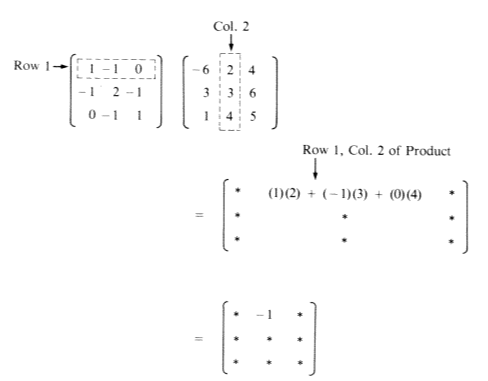
\includegraphics[width=\linewidth]{images/fig-one-matrix-product-entry.png}
\end{image}%
\tcblower
\end{figureptx}%
The computation of a product can take a considerable amount of time in comparison to the time required to add two matrices. Suppose that \(A\) and \(B\) are \(n\times n\) matrices; then \((A B)_{ij}\) is determined performing \(n\) multiplications and \(n-1\) additions. The full product takes \(n^3\) multiplications and \(n^3 - n^2\) additions. This compares with \(n^2\) additions for the sum of two \(n\times n\) matrices. The product of two 10 by 10 matrices will require 1,000 multiplications and 900 additions, clearly a job that you would assign to a computer. The sum of two matrices requires a more modest 100 additions. This analysis is based on the assumption that matrix multiplication will be done using the formula that is given in the definition. There are more advanced methods that, in theory, reduce operation counts. For example, Strassen's algorithm (\href{https://en.wikipedia.org/wiki/Strassen_algorithm}{https:\slash{}\slash{}en.wikipedia.org\slash{}wiki\slash{}Strassen\textunderscore{}algorithm}) computes the product of two \(n\) by \(n\) matrices in \(7\cdot 7^{\log _2n}-6\cdot  4^{\log _2n}\approx  7 n^{2.808}\) operations. There are practical issues involved in actually using the algorithm in many situations.  For example, round-off error can be more of a problem than with the standard formula.%
\begin{example}{A Matrix Product.}{x:example:ex-matrix-product}%
Let \(A =\left(
\begin{array}{cc}
1 & 0 \\
3 & 2 \\
-5 & 1 \\
\end{array}
\right)\), a \(3\times 2\) matrix, and let \(B =\left(
\begin{array}{c}
6 \\
1 \\
\end{array}
\right)\), a \(2\times 1\) matrix. Then \(A B\) is a \(3 \times  1\) matrix:%
\begin{equation*}
A B = \left(
\begin{array}{cc}
1 & 0 \\
3 & 2 \\
-5 & 1 \\
\end{array}
\right) \left(
\begin{array}{c}
6 \\
1 \\
\end{array}
\right) = \left(
\begin{array}{c}
1\cdot 6+0\cdot 1 \\
3 \cdot 6 + 2\cdot 1 \\
-5 \cdot 6 + 1\cdot 1 \\
\end{array}
\right) = \left(
\begin{array}{c}
6 \\
20 \\
-29 \\
\end{array}
\right)
\end{equation*}
%
\end{example}
Remarks:%
\par
%
\begin{enumerate}[label=(\arabic*)]
\item{}The product \(A B\) is defined only if \(A\) is an \(m\times n\) matrix and \(B\) is an \(n\times p\) matrix; that is, the two ``inner'' numbers must be equal. Furthermore, the order of the product matrix \(A B\) is the ``outer'' numbers, in this case \(m\times p\).%
\item{}It is wise to first determine the order of a product matrix. For example, if \(A\) is a \(3\times 2\) matrix and \(B\) is a \(2\times 2\) matrix, then \(A B\) is a \(3\times 2\) matrix of the form%
\begin{equation*}
A B =\left(
\begin{array}{cc}
c_{11} & c_{12} \\
c_{21} & c_{22} \\
c_{31} & c_{32} \\
\end{array}
\right)
\end{equation*}
Then to obtain, for example, \(c_{31}\), we multiply corresponding entries in the third row of \(A\) times the first column of \(B\) and add the results.%
\end{enumerate}
%
\begin{example}{Multiplication with a diagonal matrix.}{x:example:ex-diagonal-product}%
Let \(A =\left(
\begin{array}{cc}
-1 & 0 \\
0 & 3 \\
\end{array}
\right)\) and \(B =\left(
\begin{array}{cc}
3 & 10 \\
2 & 1 \\
\end{array}
\right)\) . Then \(A B =\left(
\begin{array}{cc}
-1\cdot 3 + 0\cdot 2 & -1\cdot 10+0\cdot 1 \\
0\cdot 3+3\cdot 2 & 0\cdot 10+3\cdot 1 \\
\end{array}
\right)= \left(
\begin{array}{cc}
-3 & -10 \\
6 & 3 \\
\end{array}
\right)\)%
\par
The net effect is to multiply the first row of \(B\) by \(-1\) and the second row of \(B\) by 3.%
\par
Note: \(B A =\left(
\begin{array}{cc}
-3 & 30 \\
-	2 & 3 \\
\end{array}
\right) \neq A B\).   The columns of \(B\) are multiplied by \(-1\) and 3 when the order is switched.%
\end{example}
Remarks:%
\par
%
\begin{itemize}[label=\textbullet]
\item{}An \(n\times n\) matrix is called a \emph{square matrix}.%
\item{}If \(A\) is a square matrix, \(A A\) is defined and is denoted by \(A^2\) , and \(A A A = A^3\), etc.%
\item{}The \(m\times n\) matrices whose entries are all 0 are denoted by \(\pmb{0}_{m\times n}\), or simply \(\pmb{ 0}\), when no confusion arises regarding the order.\label{g:notation:idm40484334432}%
\end{itemize}
%
\end{subsectionptx}
%
%
\typeout{************************************************}
\typeout{Exercises 5.1.4 Exercises}
\typeout{************************************************}
%
\begin{exercises-subsection}{Exercises}{}{Exercises}{}{}{x:exercises:exercises-5-1}
\begin{divisionexercise}{1}{}{}{g:exercise:idm40484177216}%
Let \(A=\left(
\begin{array}{cc}
1 & -1 \\
2 & 3 \\
\end{array}
\right)\), \(B =\left(
\begin{array}{cc}
0 & 1 \\
3 & -5 \\
\end{array}
\right)\) , and \(C=\left(
\begin{array}{ccc}
0 & 1 & -1 \\
3 & -2 & 2 \\
\end{array}
\right)\)%
\par
%
\begin{enumerate}[label=(\alph*)]
\item{}Compute \(A B\) and \(B A\).%
\item{}Compute \(A + B\) and \(B + A\).%
\item{}If \(c = 3\), show that \(c(A + B) = c A + c B\).%
\item{}Show that \((A B)C = A(B C)\).%
\item{}Compute \(A^2 C\).%
\item{}Compute \(B + \pmb{0}\).%
\item{}Compute \(A \pmb{0}_{2\times 2}\) and \(\pmb{0}_{2\times 2} A\), where \(\pmb{0}_{2\times 2}\) is the \(2\times 2\) zero matrix.%
\item{}Compute \(0A\), where 0 is the real number (scalar) zero.%
\item{}Let \(c = 2\) and \(d = 3\). Show that \((c + d)A = c A + d A\).%
\end{enumerate}
%
\end{divisionexercise}%
\begin{divisionexercise}{2}{}{}{g:exercise:idm40484542256}%
Let \(A = \left(
\begin{array}{ccc}
1 & 0 & 2 \\
2 & -1 & 5 \\
3 & 2 & 1 \\
\end{array}
\right)\) , \(B =\left(
\begin{array}{ccc}
0 & 2 & 3 \\
1 & 1 & 2 \\
-1 & 3 & -2 \\
\end{array}
\right)\) , and \(C=\left(
\begin{array}{cccc}
2 & 1 & 2 & 3 \\
4 & 0 & 1 & 1 \\
3 & -1 & 4 & 1 \\
\end{array}
\right)\) Compute, if possible;%
\par
%
\begin{multicols}{2}
\begin{enumerate}[label=(\alph*)]
\item{}\(A - B\)%
\item{}\(A B\)%
\item{}\(A C - B C\)%
\item{}\(A(B C)\)%
\item{}\(C A - C B\)%
\item{}\(C \left(
\begin{array}{c}
x \\
y \\
z \\
w \\
\end{array}
\right)\)%
\end{enumerate}
\end{multicols}
%
\end{divisionexercise}%
\begin{divisionexercise}{3}{}{}{g:exercise:idm40484642416}%
Let \(A =\left(
\begin{array}{cc}
2 & 0 \\
0 & 3 \\
\end{array}
\right)\) . Find a matrix \(B\) such that \(A B = I\) and \(B A = I\), where \(I = \left(
\begin{array}{cc}
1 & 0 \\
0 & 1 \\
\end{array}
\right)\).%
\end{divisionexercise}%
\begin{divisionexercise}{4}{}{}{g:exercise:idm40484676224}%
Find \(A I\) and \(B I\) where \(I\) is as in Exercise 3, where \(A = \left(
\begin{array}{cc}
1 & 8 \\
9 & 5 \\
\end{array}
\right)\) and \(B = \left(
\begin{array}{cc}
-2 & 3 \\
5 & -7 \\
\end{array}
\right)\). What do you notice?%
\end{divisionexercise}%
\begin{divisionexercise}{5}{}{}{g:exercise:idm40484727040}%
Find \(A^3\) if \(A=\left(
\begin{array}{ccc}
1 & 0 & 0 \\
0 & 2 & 0 \\
0 & 0 & 3 \\
\end{array}
\right)\) . What is \(A^{15}\) equal to?%
\end{divisionexercise}%
\begin{divisionexercise}{6}{}{}{g:exercise:idm40484890320}%
%
\begin{enumerate}[label=(\alph*)]
\item{}Determine \(I^2\) and \(I^3 \text{ if }\) \(I = \left(
\begin{array}{ccc}
1 & 0 & 0 \\
0 & 1 & 0 \\
0 & 0 & 1 \\
\end{array}
\right)\).%
\item{}What is \(I^n\) equal to for any \(n\geq 1\)?%
\item{}Prove your answer to part (b) by induction.%
\end{enumerate}
%
\end{divisionexercise}%
\begin{divisionexercise}{7}{}{}{g:exercise:idm40484938608}%
%
\begin{enumerate}[label=(\alph*)]
\item{}If%
\begin{equation*}
A =\left(
\begin{array}{cc}
2 & 1 \\
1 & -1 \\
\end{array}
\right), X =\left(
\begin{array}{c}
x_1 \\
x_2 \\
\end{array}
\right)\textrm{, and }B =\left(
\begin{array}{c}
3 \\
1 \\
\end{array}
\right),
\end{equation*}
show that \(A X =B\) is a way of expressing the system \(\begin{array}{c}2x_1 + x_2 = 3\\ x_1 - x_2= 1\\
\end{array}\)  using matrices.%
\item{}Express the following systems of equations using matrices:%
\par
%
\begin{multicols}{2}
\begin{enumerate}[label=(\roman*)]
\item{}\(\begin{array}{c}
2 x_1- x_2= 4\\
x_1+ x_2= 0\\
\end{array}\)%
\item{}\(\begin{array}{c}
x_1+ x_2+ 2 x_3= 1\\
x_1+ 2 x_2-x_3= -1\\
x_1+ 3 x_2+x_3= 5\\
\end{array}\)%
\item{}\(\begin{array}{c}
x_1+x_2\quad\quad= 3\\
\quad \quad x_2\quad\quad= 5\\
x_1 \quad \quad+ 3x_3= 6\\
\end{array} \)%
\end{enumerate}
\end{multicols}
%
\end{enumerate}
%
\end{divisionexercise}%
\begin{divisionexercise}{8}{}{}{x:exercise:exercise-bakery}%
In this exercise, we propose to show how matrix multiplication is a natural operation.  Suppose a bakery produces bread, cakes and pies every weekday, Monday through Friday. Based on past sales history, the bakery produces various numbers of each product each day, summarized in the \(5 \times 3\) matrix \(D\).  It should be noted that the order could be described as ``number of days by number of products.''   For example, on Wednesday (the third day) the number of cakes (second product in our list) that are produced  is  \(d_{3,2} = 4\).%
\begin{equation*}
D =\left(
\begin{array}{ccc}
25 & 5 & 5 \\
14 & 5 & 8 \\
20 & 4 & 15 \\
18 & 5 & 7 \\
35 & 10 & 9 \\
\end{array}
\right)
\end{equation*}
%
\par
The main ingredients of these products are flour, sugar and eggs. We assume that other ingredients are always in ample supply, but we need to be sure to have the three main ones available.   For each of the three products, The amount of each ingredient that is needed is summarized in the \(3 \times 3\), or ``number of products by number of ingredients'' matrix \(P\).  For example, to bake a cake (second product) we need \(P_{2,1}=1.5\) cups of flour (first ingredient).  Regarding units: flour and sugar are given in cups per unit of each product, while eggs are given in individual eggs per unit of each product.%
\begin{equation*}
P =\left(
\begin{array}{ccc}
2 & 0.5 & 0 \\
1.5 & 1 & 2 \\
1 & 1 & 1  \\
\end{array}
\right)
\end{equation*}
These amounts are ``made up'', so don't used them to do your own baking!%
\par
%
\begin{enumerate}[label=(\alph*)]
\item{}How many cups of flour will the bakery need every Monday?  Pay close attention to how you compute your answer and the units of each number.%
\item{}How many eggs will the bakery need every Wednesday?%
\item{}Compute the matrix product \(D P\).   What do you notice?%
\item{}Suppose the costs of ingredients are \(\$0.12\) for a cup of flour, \(\$0.15\) for a cup of sugar and \(\$0.19\) for one egg. How can this information be put into a matrix that can meaningfully be multiplied by one of the other matrices in this problem?%
\end{enumerate}
%
\end{divisionexercise}%
\end{exercises-subsection}
\end{sectionptx}
%
%
\typeout{************************************************}
\typeout{Section 5.2 Special Types of Matrices}
\typeout{************************************************}
%
\begin{sectionptx}{Special Types of Matrices}{}{Special Types of Matrices}{}{}{x:section:s-special-matrices}
%
%
\typeout{************************************************}
\typeout{Subsection 5.2.1 Diagonal Matrices}
\typeout{************************************************}
%
\begin{subsectionptx}{Diagonal Matrices}{}{Diagonal Matrices}{}{}{g:subsection:idm40484989088}
We have already investigated, in exercises in the previous section, one special type of matrix. That was the  zero matrix, and found that it behaves in matrix algebra in an analogous fashion to the real number 0; that is, as the additive identity. We will now investigate the properties of a few other special matrices.%
\begin{definition}{Diagonal Matrix.}{x:definition:def-diagonal-matrix}%
A square matrix D is called a diagonal matrix if \(d_{i j}\) = 0 whenever \(i \neq  j\).%
\end{definition}
\begin{example}{Some diagonal matrices.}{x:example:example-diagonal-matrices}%
\(A = \left(
\begin{array}{ccc}
1 & 0 & 0 \\
0 & 2 & 0 \\
0 & 0 & 5 \\
\end{array}
\right)\), \(B= \left(
\begin{array}{ccc}
3 & 0 & 0 \\
0 & 0 & 0 \\
0 & 0 & -5 \\
\end{array}
\right)\), and \(I = \left(
\begin{array}{ccc}
1 & 0 & 0 \\
0 & 1 & 0 \\
0 & 0 & 1 \\
\end{array}
\right)\) are all diagonal matrices.%
\end{example}
\end{subsectionptx}
%
%
\typeout{************************************************}
\typeout{Subsection 5.2.2 The Identity Matrix and Matrix Inverses}
\typeout{************************************************}
%
\begin{subsectionptx}{The Identity Matrix and Matrix Inverses}{}{The Identity Matrix and Matrix Inverses}{}{}{g:subsection:idm40485034768}
In the example above, the \(3\times 3\) diagonal matrix \(I\) whose diagonal entries are all 1's has the distinctive property that for any other \(3\times 3\) matrix \(A\) we have \(A I = I A = A\). For example:%
\begin{example}{Multiplying by the Identity Matrix.}{x:example:ex-matrix-identity-product}%
If \(A = \left(
\begin{array}{ccc}
1 & 2 & 5 \\
6 & 7 & -2 \\
3 & -3 & 0 \\
\end{array}
\right)\), then \(A I =\left(
\begin{array}{ccc}
1 & 2 & 5 \\
6 & 7 & -2 \\
3 & -3 & 0 \\
\end{array}
\right)\) and \(I A = \left(
\begin{array}{ccc}
1 & 2 & 5 \\
6 & 7 & -2 \\
3 & -3 & 0 \\
\end{array}
\right)\).%
\end{example}
In other words, the matrix \(I\) behaves in matrix algebra like the real number 1; that is, as a multiplicative identity. In matrix algebra, the matrix \(I\) is called simply the identity matrix. Convince yourself that if \(A\) is any \(n\times n\) matrix \(A I = I A = A\).%
\begin{definition}{Identity Matrix.}{x:definition:def-identity-matrix}%
\index{Identity Matrix}%
\label{g:notation:idm40485783136}%
The \(n\times n\) diagonal matrix \(I_n\) whose diagonal components are all 1's is called the identity matrix.  If the context is clear, we simply use \(I\).%
\end{definition}
In the set of real numbers we recall that, given a nonzero real number \(x\), there exists a real number \(y\) such that \(x y = y x
=1\). We know that real numbers commute under multiplication so that the two equations can be summarized as \(x y = 1\). Further we know that \(y =x^{-1}= \frac{1}{x}\). Do we have an analogous situation in \(M_{n\times n}(\mathbb{R})\)? Can we define the multiplicative inverse of an \(n\times n\) matrix \(A\)? It seems natural to imitate the definition of multiplicative inverse in the real numbers.%
\begin{definition}{Matrix Inverse.}{x:definition:def-matrix-inverse}%
\index{Inverse!Matrix}%
\label{g:notation:idm40485529072}%
Let \(A\) be an \(n\times n\) matrix. If there exists an \(n\times n\) matrix \(B\) such that \(A B = B A =I\), then \(B\) is a multiplicative inverse of \(A\) (called simply an inverse of \(A\)) and is denoted by \(A^{-1}\)%
\end{definition}
When we are doing computations involving matrices, it would be helpful to know that when we find \(A^{-1}\), the answer we obtain is the only inverse of the given matrix.  This would let us refer to \emph{the} inverse of a matrix.  We refrained from saying that in the definition, but the theorem below justifies it.%
\par
Remark: Those unfamiliar with the laws of matrix algebra should return to the following proof after they have familiarized themselves with the Laws of Matrix Algebra in Section 5.5.%
\begin{theorem}{Inverses are unique.}{}{x:theorem:theorem-unique-inverse}%
The inverse of an \(n\times n\) matrix A, when it exists, is unique.%
\end{theorem}
\begin{proof}{}{g:proof:idm40485581056}
Let \(A\) be an \(n\times n\) matrix. Assume to the contrary, that \(A\) has two (different) inverses, say \(B\) and \(C\). Then%
\begin{equation*}
\begin{split}
B &= B I\quad \textrm{    Identity property of } I\\
& =B (A C)\quad  \textrm{    Assumption that } C \textrm{ is an inverse of } A\\
& = (B A) C \quad  \textrm{    Associativity of matrix multiplication}\\
& = I C\quad   \textrm{     Assumption that } B \textrm{ is an inverse of } A\\
& = C \quad  \textrm{     Identity property of } I
\end{split}\qedhere
\end{equation*}
%
\end{proof}
Let \(A =\left(
\begin{array}{cc}
2 & 0 \\
0 & 3  \\
\end{array}
\right)\) .  What is \(A^{-1}\) ? Without too much difficulty, by trial and error, we determine that \(A^{-1}= \left(
\begin{array}{cc}
\frac{1}{2} & 0 \\
0 & \frac{1}{3} \\
\end{array}
\right)\) . This might lead us to guess that the inverse is found by taking the reciprocal of all nonzero entries of a matrix. Alas, it isn't that easy!%
\par
If \(A =\left(
\begin{array}{cc}
1 & 2 \\
-3 & 5 \\
\end{array}
\right)\) , the ``reciprocal rule'' would tell us that the inverse of \(A\) is \(B=\left(
\begin{array}{cc}
1 & \frac{1}{2} \\
\frac{-1}{3} & \frac{1}{5} \\
\end{array}
\right)\). Try computing \(A B\) and you will see that you don't get the identity matrix.  So, what \emph{is} \(A^{-1}\)? In order to understand more completely the notion of the inverse of a matrix, it would be beneficial to have a formula that would enable us to compute the inverse of at least a \(2\times 2\) matrix. To do this, we introduce the definition of the determinant of a \(2\times 2\) matrix.%
\begin{definition}{Determinant of a 2 by 2 matrix.}{x:definition:determinant-2by2}%
\label{g:notation:idm40475342784}%
Let \(A =\left(
\begin{array}{cc}
a & b \\
c & d \\
\end{array}
\right)\). The determinant of \(A\) is the number \(\det  A = a d - b c\).%
\end{definition}
In addition to \(\det  A\), common notation for the determinant of matrix \(A\) is \(\lvert A \rvert\).  This is particularly common when writing out the whole matrix, which case we would write \(\left|
\begin{array}{cc}
a & b \\
c & d \\
\end{array}
\right|\) for the determinant of the general \(2 \times 2\) matrix.%
\begin{example}{Some determinants of two by two matrices.}{x:example:ex-some-determinants}%
If \(A =\left(
\begin{array}{cc}
1 & 2 \\
-3 & 5 \\
\end{array}
\right)\)  then \(\det  A = 1\cdot 5 -2\cdot  (-3)=11\). If \(B =\left(
\begin{array}{cc}
1 & 2 \\
2 & 4 \\
\end{array}
\right)\)  then \(\det  B = 1\cdot 4 -2\cdot 2=0.\)%
\end{example}
\begin{theorem}{Inverse of 2 by 2 matrix.}{}{x:theorem:theorem-inverse-two-by-two}%
Let \(A =\left(
\begin{array}{cc}
a & b \\
c & d \\
\end{array}
\right)\).  If \(\det  A\neq  0\), then \(A^{-1} =\frac{1}{\det  A}\left(
\begin{array}{cc}
d & -b \\
-c & a \\
\end{array}
\right)\).%
\end{theorem}
\begin{proof}{}{g:proof:idm40484483104}
See Exercise 4 at the end of this section.%
\end{proof}
\begin{example}{Finding Inverses.}{x:example:ex-finding-inverses}%
Can we find the inverses of the matrices in \hyperref[x:example:ex-some-determinants]{Example~{\xreffont\ref{x:example:ex-some-determinants}}}? If \(A =\left(
\begin{array}{cc}
1 & 2 \\
-3 & 5 \\
\end{array}
\right)\)  then%
\begin{equation*}
A^{-1}= \frac{1}{11}\left(
\begin{array}{cc}
5 & -2 \\
3 & 1 \\
\end{array}
\right)=\left(
\begin{array}{cc}
\frac{5}{11} & -\frac{2}{11} \\
\frac{3}{11} & \frac{1}{11} \\
\end{array}
\right)
\end{equation*}
The reader should verify that \(A A^{-1}=A^{-1}A = I\).%
\par
The second matrix, \(B\), has a determinant equal to zero. If we tried to apply the formula in \hyperref[x:theorem:theorem-inverse-two-by-two]{Theorem~{\xreffont\ref{x:theorem:theorem-inverse-two-by-two}}}, we would be dividing by zero. For this reason, the formula can't be applied and in fact \(B^{-1}\) does not exist.%
\end{example}
Remarks:%
\begin{itemize}[label=\textbullet]
\item{}In general, if \(A\) is a \(2\times 2\) matrix and if \(\det  A = 0\), then \(A^{-1}\) does not exist.%
\item{}A formula for the inverse of \(n\times n\) matrices \(n\geq  3\) can be derived that also involves \(\det  A\). Hence, in general, if the determinant of a matrix is zero, the matrix does not have an inverse. However the formula for even a \(3 \times  3\) matrix is very long and is not the most efficient way to compute the inverse of a matrix.%
\item{}In Chapter 12 we will develop a technique to compute the inverse of a higher-order matrix, if it exists.%
\item{}Matrix inversion comes first in the hierarchy of matrix operations; therefore, \(A B^{-1}\) is \(A (B^{-1})\).%
\end{itemize}
%
\end{subsectionptx}
%
%
\typeout{************************************************}
\typeout{Exercises 5.2.3 Exercises}
\typeout{************************************************}
%
\begin{exercises-subsection}{Exercises}{}{Exercises}{}{}{x:exercises:exercises-5-4}
\begin{divisionexercise}{1}{}{}{g:exercise:idm40485081600}%
For the given matrices \(A\) find \(A^{-1}\) if it exists and verify that \(A A^{-1}=A^{-1}A = I\).  If \(A^{-1}\) does not exist explain why.%
\par
%
\begin{enumerate}[label=(\alph*)]
\item{}\(\displaystyle A = \left(
\begin{array}{cc}
1 & 3 \\
2 & 1 \\
\end{array}
\right)\)%
\item{}\(\displaystyle A=\left(
\begin{array}{cc}
6 & -3 \\
8 & -4 \\
\end{array}
\right)\)%
\item{}\(\displaystyle A = \left(
\begin{array}{cc}
1 & -3 \\
0 & 1 \\
\end{array}
\right)\)%
\item{}\(\displaystyle A = \left(
\begin{array}{cc}
1 & 0 \\
0 & 1 \\
\end{array}
\right)\)%
\item{}Use the definition of the inverse of a matrix to find \(A^{-1}\): \(A=\left(
\begin{array}{ccc}
3 & 0 & 0 \\
0 & \frac{1}{2} & 0 \\
0 & 0 & -5 \\
\end{array}
\right)\)%
\end{enumerate}
%
\end{divisionexercise}%
\begin{divisionexercise}{2}{}{}{g:exercise:idm40485452560}%
For the given matrices \(A\) find \(A^{-1}\) if it exists and verify that \(A A^{-1}=A^{-1}A = I\). If \(A^{-1}\) does not exist explain why.%
\par
%
\begin{enumerate}[label=(\alph*)]
\item{}\(\displaystyle A =\left(
\begin{array}{cc}
2 & -1 \\
-1 & 2 \\
\end{array}
\right)\)%
\item{}\(\displaystyle A = \left(
\begin{array}{cc}
0 & 1 \\
0 & 2 \\
\end{array}
\right)\)%
\item{}\(\displaystyle A= \left(
\begin{array}{cc}
1 & c \\
0 & 1 \\
\end{array}
\right)\)%
\item{}\(A = \left(
\begin{array}{cc}
a & b \\
b & a \\
\end{array}
\right)\), where \(\lvert a \rvert \neq \lvert b \rvert\).%
\end{enumerate}
%
\end{divisionexercise}%
\begin{divisionexercise}{3}{}{}{x:exercise:prob-5-2-3}%
%
\begin{enumerate}[label=(\alph*)]
\item{}Let \(A = \left(
\begin{array}{cc}
2 & 3 \\
1 & 4 \\
\end{array}
\right)\) and \(B =\left(
\begin{array}{cc}
3 & -3 \\
2 & 1 \\
\end{array}
\right)\). Verify that \((A B)^{-1}= B^{-1}A^{-1}\).%
\item{}Let \(A\) and \(B\) be \(n\times n\) invertible matrices. Prove that \((A B)^{-1}= B^{-1}A^{-1}\). Why is the right side of the above statement written ``backwards''? Is this necessary? Hint: Use \hyperref[x:theorem:theorem-unique-inverse]{Theorem~{\xreffont\ref{x:theorem:theorem-unique-inverse}}}%
\end{enumerate}
%
\end{divisionexercise}%
\begin{divisionexercise}{4}{}{}{g:exercise:idm40484373584}%
Let \(A =\left(
\begin{array}{cc}
a & b \\
c & d \\
\end{array}
\right)\). Derive the formula for \(A^{-1}\).%
\end{divisionexercise}%
\begin{divisionexercise}{5}{Linearity of Determinants.}{}{x:exercise:prob-5-2-5}%
%
\begin{enumerate}[label=(\alph*)]
\item{}Let \(A\) and \(B\) be 2-by-2 matrices. Show that \(\det (A B) =(\det  A)(\det  B)\).%
\item{}It can be shown that the statement in part (a) is true for all \(n\times n\) matrices. Let \(A\) be any invertible \(n\times n\) matrix. Prove that \(\det \left(A^{-1}\right) =(\det  A)^{-1}\). Note: The determinant of the identity matrix \(I_n\) is 1 for all \(n\).%
\item{}Verify that the equation in part (b) is true for the matrix in exercise 1(a) of this section.%
\end{enumerate}
%
\end{divisionexercise}%
\begin{divisionexercise}{6}{}{}{g:exercise:idm40484925248}%
Prove by induction that for \(n \geq 1\), \(\left(
\begin{array}{cc}
a & 0 \\
0 & b \\
\end{array}
\right)^n= \left(
\begin{array}{cc}
a^n & 0 \\
0 & b^n \\
\end{array}
\right)\).%
\end{divisionexercise}%
\begin{divisionexercise}{7}{}{}{g:exercise:idm40484968032}%
Use the assumptions in \hyperlink{x:exercise:prob-5-2-5}{Exercise~{\xreffont 5.2.3.5}} to prove by induction that if \(n \geq 1\), \(\det \left(A^n\right) = (\det  A)^n\).%
\end{divisionexercise}%
\begin{divisionexercise}{8}{}{}{g:exercise:idm40485160560}%
Prove: If the determinant of a matrix \(A\) is zero, then \(A\) does not have an inverse. Hint: Use the indirect method of proof and exercise 5.%
\end{divisionexercise}%
\begin{divisionexercise}{9}{}{}{g:exercise:idm40474735136}%
%
\begin{enumerate}[label=(\alph*)]
\item{}Let \(A, B, \textrm{ and } D\) be \(n\times n\) matrices. Assume that \(B\) is invertible. If \(A = B D B^{-1}\) , prove by induction that \(A^m= B D^m B^{-1}\) is true for \(m \geq  1\).%
\item{}Given that \(A = \left(
\begin{array}{cc}
-8 & 15 \\
-6 & 11 \\
\end{array}
\right) = B \left(
\begin{array}{cc}
1 & 0 \\
0 & 2 \\
\end{array}
\right) B^{-1}\) where \(B=\left(
\begin{array}{cc}
5 & 3 \\
3 & 2 \\
\end{array}
\right)\) what is \(A^{10}\)?%
\end{enumerate}
%
\end{divisionexercise}%
\end{exercises-subsection}
\end{sectionptx}
%
%
\typeout{************************************************}
\typeout{Section 5.3 Laws of Matrix Algebra}
\typeout{************************************************}
%
\begin{sectionptx}{Laws of Matrix Algebra}{}{Laws of Matrix Algebra}{}{}{x:section:s-laws-of-matrix-algebra}
\index{Laws of Matrix Algebra}%
%
%
\typeout{************************************************}
\typeout{Subsection 5.3.1 The Laws}
\typeout{************************************************}
%
\begin{subsectionptx}{The Laws}{}{The Laws}{}{}{g:subsection:idm40475351296}
The following is a summary of the basic laws of matrix operations. Assume that the indicated operations are defined; that is, that the orders of the matrices \(A\), \(B\) and \(C\) are such that the operations make sense.%
\begin{tableptx}{\textbf{Laws of Matrix Algebra}}{x:table:table-matrix-laws}{}%
\centering
{\tabularfont%
\begin{tabular}{cc}
(1) Commutative Law of Addition&\(A + B = B + A\)\tabularnewline[0pt]
(2) Associative Law of Addition&\(A + (B + C) = (A + B) + C\)\tabularnewline[0pt]
(3) Distributive Law of a Scalar over Matrices&\(c(A + B) = c A + c B\), where \(c \in  \mathbb{R}\).\tabularnewline[0pt]
(4) Distributive Law of Scalars over a Matrix&\(\left(c_1 + c_2 \right)A = c_1A +c_2 A\), where \(c_1, c_2 \in  \mathbb{R}\).\tabularnewline[0pt]
(5) Associative Law of Scalar Multiplication&\(c_1 \left(c_2 A\right) =\left(c_1 \cdot c_2 \right)A\), where \(c_1, c_2 \in  \mathbb{R}\).\tabularnewline[0pt]
(6) Zero Matrix Annihilates all Products&\(\pmb{0}A = \pmb{0}\), where \(\pmb{0}\) is the zero matrix.\tabularnewline[0pt]
(7) Zero Scalar Annihilates all Products&\(0 A =\pmb{0}\), where 0 on the left is the scalar zero.\tabularnewline[0pt]
(8) Zero Matrix is an identity for Addition&\(A + \pmb{0} = A\).\tabularnewline[0pt]
(9) Negation produces additive inverses&\(A + (-1)A = \pmb{0}\).\tabularnewline[0pt]
(10) Right Distributive Law of Matrix Multiplication&\(A(B + C) = A B + A C\).\tabularnewline[0pt]
(11) Left  Distributive Law of Matrix Multiplication&\((B + C)A = B A + C A\).\tabularnewline[0pt]
(12) Associative Law of Multiplication&\(A(B C) = (A B)C\).\tabularnewline[0pt]
(13) Identity Matrix is a Multiplicative Identity&\(I A = A\) and \(A I = A\).\tabularnewline[0pt]
(14) Involution Property of Inverses&If \(A^{-1}\) exists,\(\left(A^{-1} \right)^{-1} = A\).\tabularnewline[0pt]
(15) Inverse of Product Rule&If \(A^{-1}\) and \(B^{-1}\) exist, \((A B)^{-1}= B^{-1}A^{-1}\)
\end{tabular}
}%
\end{tableptx}%
\end{subsectionptx}
%
%
\typeout{************************************************}
\typeout{Subsection 5.3.2 Commentary}
\typeout{************************************************}
%
\begin{subsectionptx}{Commentary}{}{Commentary}{}{}{g:subsection:idm40485219216}
\begin{example}{More Precise Statement of one Law.}{x:example:ex-statement-precise}%
If we wished to write out each of the above laws more completely, we would specify the orders of the matrices. For example, Law 10 should read:%
\begin{quote}%
Let \(A\), \(B\), and \(C\) be \(m\times n\), \(n\times p\), and \(n\times p\) matrices, respectively, then \(A(B + C) = A B + A C\)%
\end{quote}
\end{example}
Remarks:%
\par
%
\begin{itemize}[label=\textbullet]
\item{}Notice the absence of the ``law'' \(A B = B A\). Why?%
\item{}Is it really necessary to have both a right (No. 11) and a left (No. 10) distributive law? Why?%
\end{itemize}
%
\end{subsectionptx}
%
%
\typeout{************************************************}
\typeout{Exercises 5.3.3 Exercises}
\typeout{************************************************}
%
\begin{exercises-subsection}{Exercises}{}{Exercises}{}{}{x:exercises:exercises-5-5}
\begin{divisionexercise}{1}{}{}{g:exercise:idm40475348832}%
Rewrite the above laws specifying as in \hyperref[x:example:ex-statement-precise]{Example~{\xreffont\ref{x:example:ex-statement-precise}}} the orders of the matrices.%
\end{divisionexercise}%
\begin{divisionexercise}{2}{}{}{g:exercise:idm40475630864}%
Verify each of the Laws of Matrix Algebra using examples.%
\end{divisionexercise}%
\begin{divisionexercise}{3}{}{}{g:exercise:idm40464154080}%
Let \(A = \left(
\begin{array}{cc}
1 & 2 \\
0 & -1 \\
\end{array}
\right)\), \(B= \left(
\begin{array}{ccc}
3 & 7 & 6 \\
2 & -1 & 5 \\
\end{array}
\right)\), and \(C= \left(
\begin{array}{ccc}
0 & -2 & 4 \\
7 & 1 & 1 \\
\end{array}
\right)\). Compute the following as efficiently as possible by using any of the Laws of Matrix Algebra:%
\par
%
\begin{enumerate}[label=(\alph*)]
\item{}\(A B + A C\)%
\item{}\(A^{-1}\)%
\item{}\(A(B + C)\)%
\item{}\(\left(A^2\right)^{-1}\)%
\item{}\((C + B)^{-1}A^{-1}\)%
\end{enumerate}
%
\end{divisionexercise}%
\begin{divisionexercise}{4}{}{}{g:exercise:idm40464145280}%
Let \(A =\left(
\begin{array}{cc}
7 & 4 \\
2 & 1 \\
\end{array}
\right)\) and \(B =\left(
\begin{array}{cc}
3 & 5 \\
2 & 4 \\
\end{array}
\right)\). Compute the following as efficiently as possible by using any of the Laws of Matrix Algebra:%
\par
%
\begin{enumerate}[label=(\alph*)]
\item{}\(A B\)%
\item{}\(A + B\)%
\item{}\(A^2 + A B + B A + B ^2\)%
\item{}\(B^{-1}A^{-1}\)%
\item{}\(A^2 + A B\)%
\end{enumerate}
%
\end{divisionexercise}%
\begin{divisionexercise}{5}{}{}{g:exercise:idm40464139744}%
Let \(A\) and \(B\) be \(n\times n\) matrices of real numbers. Is \(A^2-B^2= (A-B)(A+B)\)?  Explain.%
\end{divisionexercise}%
\end{exercises-subsection}
\end{sectionptx}
%
%
\typeout{************************************************}
\typeout{Section 5.4 Matrix Oddities}
\typeout{************************************************}
%
\begin{sectionptx}{Matrix Oddities}{}{Matrix Oddities}{}{}{x:section:s-matrix-oddities}
\index{Matrix Oddities}%
%
%
\typeout{************************************************}
\typeout{Subsection 5.4.1 Dissimilarities with elementary algebra}
\typeout{************************************************}
%
\begin{subsectionptx}{Dissimilarities with elementary algebra}{}{Dissimilarities with elementary algebra}{}{}{g:subsection:idm40464136608}
We have seen that matrix algebra is similar in many ways to elementary algebra. Indeed, if we want to solve the matrix equation \(A X = B\) for the unknown \(X\), we imitate the procedure used in elementary algebra for solving the equation \(a x = b\). One assumption we need is that \(A\) is a square matrix that has an inverse.  Notice how exactly the same properties are used in the following detailed solutions of both equations.%
\begin{tableptx}{\textbf{}}{g:table:idm40464134128}{}%
\centering
{\tabularfont%
\begin{tabular}{ccc}
Equation in the algebra of real numbers&&Equation in  matrix algebra\tabularnewline[0pt]
\(a x = b\)&&\(A X = B\)\tabularnewline[0pt]
\(a^{-1}(a x) =a^{-1}b\) if \(a \neq  0\)&&\(A^{-1}(A X) = A^{-1}B\) if \(A^{-1 }\) exists\tabularnewline[0pt]
\(\left(a^{-1} a\right)x = a^{-1} b\)&Associative Property&\(\left(A^{-1} A\right)X = A^{-1} B\)\tabularnewline[0pt]
\(1x = a^{-1} b\)&Inverse Property&\(I X = A^{-1} B\)\tabularnewline[0pt]
\(x = a^{-1} b\)&Identity Property&\(X = A^{-1} B\)
\end{tabular}
}%
\end{tableptx}%
Certainly the solution process for solving \(A X = B\) is the same as that of solving \(a x = b\).%
\par
The solution of \(x a = b\) is \(x = b a^{-1} = a^{-1}b\). In fact, we usually write the solution of both equations as  \(x =\frac{b}{a}\). In matrix algebra, the solution of \(X A = B\) is \(X = B A^{-1}\) , which is not necessarily equal to \(A^{-1} B\). So in matrix algebra, since the commutative law (under multiplication) is not true, we have to be more careful in the methods we use to solve equations.%
\par
It is clear from the above that if we wrote the solution of \(A X = B\) as \(X=\frac{B}{A}\), we would not know how to interpret \(\frac{B}{A}\). Does it mean \(A^{-1} B\) or \(B A^{-1}\)?  Because of this, \(A^{-1}\) is never written as \(\frac{I}{A}\).%
\begin{observation}{Matrix Oddities.}{x:observation:ss-matrix-oddities}%
Some of the main dissimilarities between matrix algebra and elementary algebra are that in matrix algebra:%
\par
%
\begin{enumerate}[label=(\arabic*)]
\item{}\(A B\) may be different from \(B A\).%
\item{}There exist matrices \(A\) and \(B\) such that \(A B = \pmb{0}\), and yet \(A\neq \pmb{0}\) and \(B\neq \pmb{0}\).%
\item{}There exist matrices \(A\) where \(A \neq  \pmb{0}\), and yet \(A^2 = \pmb{0}\).%
\item{}There exist matrices \(A\) where \(A^2=A\) with \(A\neq I\) and \(A\neq \pmb{0}\)%
\item{}There exist matrices \(A\) where \(A^2=I\), where \(A\neq I\) and \(A\neq -I\)%
\end{enumerate}
%
\end{observation}
\end{subsectionptx}
%
%
\typeout{************************************************}
\typeout{Exercises 5.4.2 Exercises}
\typeout{************************************************}
%
\begin{exercises-subsection}{Exercises}{}{Exercises}{}{}{x:exercises:exercises-5-6}
\begin{divisionexercise}{1}{}{}{g:exercise:idm40464108736}%
Discuss each of the ``Matrix Oddities'' with respect to elementary algebra.%
\end{divisionexercise}%
\begin{divisionexercise}{2}{}{}{g:exercise:idm40464097776}%
Determine \(2\times 2\) matrices which show that each of the ``Matrix Oddities'' are true.%
\end{divisionexercise}%
\begin{divisionexercise}{3}{}{}{g:exercise:idm40464094192}%
Prove or disprove the following implications.%
\par
%
\begin{enumerate}[label=(\alph*)]
\item{}\(A^2= A\) and \(\det  A \neq  0 \Rightarrow  A =I\)%
\item{}\(A^2 = I \textrm{ and } \det A \neq  0 \Rightarrow  A = I \textrm{ or } A = -I\).%
\end{enumerate}
%
\end{divisionexercise}%
\begin{divisionexercise}{4}{}{}{g:exercise:idm40464088016}%
Let \(M_{n\times n}(\mathbb{R})\) be the set of real \(n\times n\) matrices. Let \(P \subseteq  M_{n\times n}(\mathbb{R})\) be the subset of matrices defined by \(A \in  P\) if and only if \(A^2 = A\). Let \(Q \subseteq  P\) be defined by \(A\in Q\) if and only if \(\det A \neq  0\).%
\par
%
\begin{enumerate}[label=(\alph*)]
\item{}Determine the cardinality of \(Q\).%
\item{}Consider the special case \(n = 2\) and prove that a sufficient condition for \(A \in  P \subseteq  M_{2\times 2}(\mathbb{R})\) is that \(A\) has a zero determinant (i.e., \(A\) is singular) and \(tr(A) = 1\) where \(tr(A) = a_{11}+ a _{22}\) is the sum of the main diagonal elements of \(A\).%
\item{}Is the condition of part b a necessary condition?%
\end{enumerate}
%
\end{divisionexercise}%
\begin{divisionexercise}{5}{}{}{g:exercise:idm40464079504}%
Write each of the following systems in the form \(A X = B\), and then solve the systems using matrices.%
\par
%
\begin{multicols}{2}
\begin{enumerate}[label=(\alph*)]
\item{}\(\begin{array}{c}2x_1+x_2=3\\
x_1-x_2= 1\\
\end{array}\)%
\item{}\(\begin{array}{c}2x_1-x_2=4\\
x_1 -x_2= 0\\
\end{array}\)%
\item{}\(\displaystyle \begin{array}{c}2x_1+x_2=1\\
x_1 -x_2= 1\\
\end{array}\)%
\item{}\(\begin{array}{c}2x_1+x_2=1\\
x_1 -x_2= -1\\
\end{array}\)%
\item{}\(\begin{array}{c}3x_1+2x_2=1 \\
6 x_1 +4x_2= -1\\
\end{array}\)%
\end{enumerate}
\end{multicols}
%
\end{divisionexercise}%
\begin{divisionexercise}{6}{}{}{g:exercise:idm40475311520}%
Recall that \(p(x) = x^2- 5x + 6\) is called a polynomial, or more specifically, a polynomial over \(\mathbb{R}\), where the coefficients are elements of \(\mathbb{R}\) and \(x \in  \mathbb{R}\). Also, think of the method of solving, and solutions of, \(x^2- 5x + 6= 0\). We would like to define the analogous situation for \(2\times 2\) matrices. First define where \(A\) is a \(2\times 2\) matrix \(p(A) =
A^2 - 5A + 6I\). Discuss the method of solving and the solutions of \(A^2 - 5A + 6I=\pmb{0}\).%
\end{divisionexercise}%
\begin{divisionexercise}{7}{}{}{g:exercise:idm40475310912}%
For those who know calculus:%
\par
%
\begin{enumerate}[label=(\alph*)]
\item{}Write the series expansion for \(e^a\) centered around \(a=0\).%
\item{}Use the idea of exercise 6 to write what would be a plausible definition of \(e^A\) where \(A\) is an \(n \times  n\) matrix.%
\item{}If \(A=\left(
\begin{array}{cc}
1 & 1 \\
0 & 0 \\
\end{array}
\right)\) and \(B =\left(
\begin{array}{cc}
0 & -1 \\
0 & 0 \\
\end{array}
\right)\) , use the series in part (b) to show that \(e^A= \left(
\begin{array}{cc}
e & e-1 \\
0 & 1 \\
\end{array}
\right)\)and \(e^B= \left(
\begin{array}{cc}
1 & -1 \\
0 & 1 \\
\end{array}
\right)\).%
\item{}Show that \(e^Ae^B\neq e^Be^A\).%
\item{}Show that  \(e^{A+B}= \left(
\begin{array}{cc}
e & 0 \\
0 & 1 \\
\end{array}
\right)\).%
\item{}Is \(e^Ae^B=e^{A+B}\)?%
\end{enumerate}
%
\end{divisionexercise}%
\end{exercises-subsection}
\end{sectionptx}
\end{chapterptx}
%
%
\typeout{************************************************}
\typeout{Chapter 6 Relations}
\typeout{************************************************}
%
\begin{chapterptx}{Relations}{}{Relations}{}{}{x:chapter:chapter_6}
\begin{introduction}{}%
\begin{poem}%
\poemTitle{adjacency matrix}
\begin{stanza}
\poemlineleft{An \terminology{adjacency matrix} will show}
\poemlineleft{Where the edges 'tween vertices go.}
\poemlineleft{For a nice simple graph}
\poemlineleft{You can cut through the chaff:}
\poemlineleft{Noughts and ones in symmetrical flow.}
\end{stanza}
\poemauthorleft{psheil, The Omnificent English Dictionary In Limerick Form}
\end{poem}
One understands a set of objects completely only if the structure of that set is made clear by the interrelationships between its elements. For example, the individuals in a crowd can be compared by height, by age, or through any number of other criteria. In mathematics, such comparisons are called relations. The goal of this chapter is to develop the language, tools, and concepts of relations.%
\end{introduction}%
%
%
\typeout{************************************************}
\typeout{Section 6.1 Basic Definitions}
\typeout{************************************************}
%
\begin{sectionptx}{Basic Definitions}{}{Basic Definitions}{}{}{x:section:s-basic-definitions}
\begin{introduction}{}%
In Chapter 1 we introduced the concept of the Cartesian product of sets. Let's assume that a person owns three shirts and two pairs of slacks. More precisely, let \(A = \{\textrm{blue shirt}, \textrm{tan shirt}, \textrm{mint green shirt}\}\) and \(B = \{\textrm{grey slacks}, \textrm{tan slacks}\}\). Then \(A\times B\) is the set of all six possible combinations of shirts and slacks that the individual could wear. However, an individual may wish to restrict himself or herself to combinations which are color coordinated, or ``related.'' This may not be all possible pairs in \(A\times B\) but will certainly be a subset of \(A\times B\). For example, one such subset may be%
\begin{equation*}
\{(\textrm{blue shirt}, \textrm{grey slacks}), (\textrm{blue shirt},  \textrm{tan slacks}), (\textrm{mint green shirt}, \textrm{tan slacks})\}.
\end{equation*}
%
\end{introduction}%
%
%
\typeout{************************************************}
\typeout{Subsection 6.1.1 Relations between two sets}
\typeout{************************************************}
%
\begin{subsectionptx}{Relations between two sets}{}{Relations between two sets}{}{}{g:subsection:idm40475057344}
\begin{definition}{Relation.}{x:definition:Relation}%
\index{Relation}%
Let \(A\) and \(B\) be sets. A relation from \(A\) into \(B\) is any subset of \(A\times B\).%
\end{definition}
\begin{example}{A simple example.}{x:example:ex-simple-relation}%
Let \(A = \{1, 2, 3\}\) and \(B = \{4, 5\}\). Then \(\{(1, 4), (2, 4), (3, 5)\}\) is a relation from \(A\) into \(B\). Of course, there are many others we could describe; 64, to be exact.%
\end{example}
\begin{example}{Divisibility Example.}{x:example:ex-divides-example}%
Let \(A = \{2, 3, 5, 6\}\) and define a relation \(r\) from \(A\) into \(A\) by \((a, b) \in r\) if and only if \(a\) divides evenly into \(b\). The set of pairs that qualify for membership is \(r = \{(2, 2), (3, 3), (5, 5), (6, 6), (2, 6), (3, 6)\}\).%
\end{example}
\end{subsectionptx}
%
%
\typeout{************************************************}
\typeout{Subsection 6.1.2 Relations on a Set}
\typeout{************************************************}
%
\begin{subsectionptx}{Relations on a Set}{}{Relations on a Set}{}{}{g:subsection:idm40475046720}
\begin{definition}{Relation on a Set.}{x:definition:relation-on-a-set}%
\index{Relation on a Set}%
A relation from a set \(A\) into itself is called a relation on \(A\).%
\end{definition}
The relation ``divides'' in \hyperref[x:example:ex-divides-example]{Example~{\xreffont\ref{x:example:ex-divides-example}}} will appear throughout the book. Here is a general definition on the whole set of integers.%
\begin{definition}{Divides.}{x:definition:Divides}%
\index{Divides}%
\label{g:notation:idm40475038656}%
Let \(a, b \in \mathbb{Z}\), \(a \neq 0\). We say that \(a\) divides \(b\), denoted \(a \mid b\),  if and only if there exists an integer \(k\) such that \(a k = b\).%
\end{definition}
Be very careful in writing about the relation ``divides.''  The vertical line symbol use for this relation, if written carelessly, can look like division.  While \(a \mid b\) is either true or false, \(a/b\) is a number.%
\par
Based on the equation \(a k = b\), we can say that \(a|b\) is equivalent to \(k= \frac{b}{a}\), or \(a\) divides evenly into \(b\). In fact the ``divides'' is short for ``divides evenly into.'' You might find the equation \(k= \frac{b}{a}\) initially easier to understand, but in the long run we will find the equation \(a k = b\) more convenient.%
\par
Sometimes it is helpful to illustrate a relation with a graph. Consider \hyperref[x:example:ex-simple-relation]{Example~{\xreffont\ref{x:example:ex-simple-relation}}}.  A graph of \(r\) can be drawn as in \hyperref[x:figure:graph-6-1-1-relation]{Figure~{\xreffont\ref{x:figure:graph-6-1-1-relation}}}. The arrows indicate that 1 is related to 4 under \(r\). Also, 2 is related to 4 under \(r\), and 3 is related to 5, while the upper arrow denotes that \(r\) is a relation from the whole set \(A\) into the set \(B\).%
\begin{figureptx}{The graph of a relation}{x:figure:graph-6-1-1-relation}{}%
\begin{image}{0.125}{0.75}{0.125}%
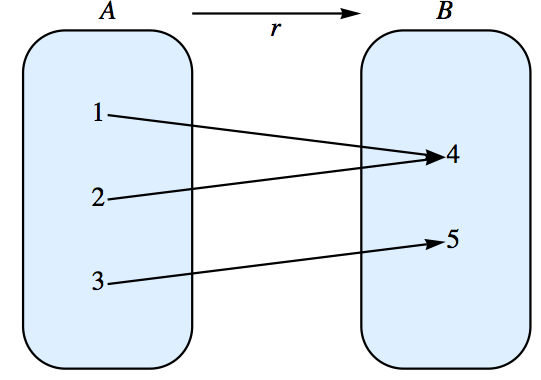
\includegraphics[width=\linewidth]{images/graph-6-1-relation-graph.png}
\end{image}%
\tcblower
\end{figureptx}%
A typical element in a relation \(r\) is an ordered pair \((x, y)\). In some cases, \(r\) can be described by actually listing the pairs which are in \(r\), as in the previous examples. This may not be convenient if \(r\) is relatively large. Other notations are used with certain well-known relations. Consider the ``less than or equal'' relation on the real numbers. We could define it as a set of ordered pairs this way:%
\begin{equation*}
\le = \{(x, y) | x \leq  y\}
\end{equation*}
However, the notation \(x \leq  y\) is clear and self-explanatory; it is a more natural, and hence preferred, notation to use than \((x, y) \in \le\).%
\par
Many of the relations we will work with ``resemble'' the relation \(\leq\), so \(x s y\) is a common way to express the fact that \(x\) is related to \(y\) through the relation \(s\).%
\par
\emph{Relation Notation}\index{Relation Notation} Let \(s\) be a relation from a set \(A\) into a set \(B\). Then the fact that \((x, y) \in s\) is frequently written \(x s y\).\label{g:notation:idm40475013536}%
\end{subsectionptx}
%
%
\typeout{************************************************}
\typeout{Subsection 6.1.3 Composition of Relations}
\typeout{************************************************}
%
\begin{subsectionptx}{Composition of Relations}{}{Composition of Relations}{}{}{g:subsection:idm40475043264}
With \(A = \{2, 3, 5, 8\}\), \(B = \{4, 6, 16\}\), and \(C = \{1, 4, 5, 7\}\), let \(r\) be the relation ``divides,'' from \(A\) into \(B\), and let \(s\) be the relation \(\leq\) from \(B\) into \(C\). So \(r = \{(2, 4), (2, 6), (2,16), (3, 6), (8, 16)\}\) and \(s = \{(4, 4), (4, 5), (4, 7), (6, 7)\}\).%
\par
Notice that in \hyperref[x:figure:graph-6-1-relation-composition]{Figure~{\xreffont\ref{x:figure:graph-6-1-relation-composition}}} that we can, for certain elements of \(A\), go through elements in \(B\) to results in \(C\). That is:%
\begin{tableptx}{\textbf{}}{x:table:table-relation-composition-example}{}%
\centering
{\tabularfont%
\begin{tabular}{c}
\(2 | 4 \textrm{ and } 4 \leq  4\)\tabularnewline[0pt]
\(2 | 4 \textrm{ and } 4 \leq  5\)\tabularnewline[0pt]
\(2 | 4 \textrm{ and } 4 \leq  7\)\tabularnewline[0pt]
\(2| 6 \textrm{ and } 6 \leq 7\)\tabularnewline[0pt]
\(3| 6 \textrm{ and } 6 \leq  7\)
\end{tabular}
}%
\end{tableptx}%
\begin{figureptx}{Relation Composition - a graphical view}{x:figure:graph-6-1-relation-composition}{}%
\begin{image}{0.075}{0.85}{0.075}%
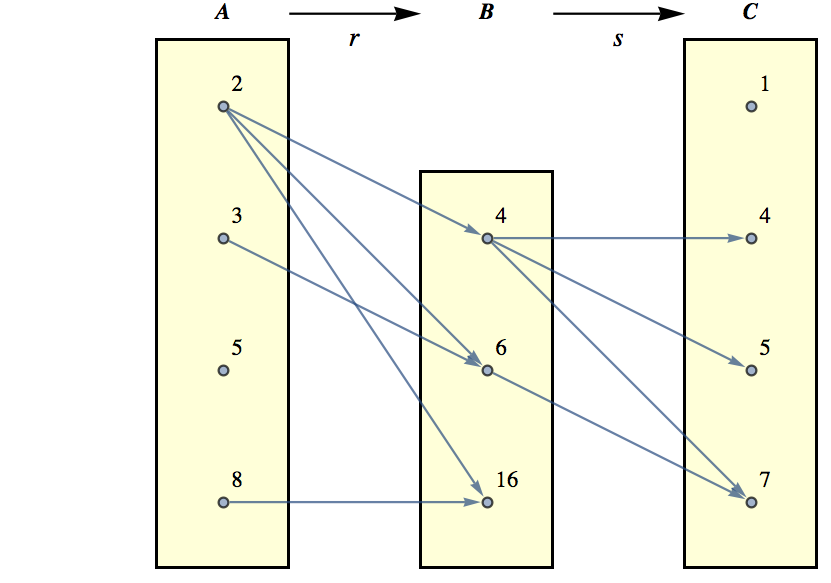
\includegraphics[width=\linewidth]{images/graph-6-1-relation-composition.png}
\end{image}%
\tcblower
\end{figureptx}%
Based on this observation, we can define a new relation, call it \(rs\), from \(A\) into \(C\). In order for \((a, c)\) to be in \(rs\), it must be possible to travel along a path in \hyperref[x:figure:graph-6-1-relation-composition]{Figure~{\xreffont\ref{x:figure:graph-6-1-relation-composition}}} from \(a\) to \(c\). In other words, \((a, c) \in rs\) if and only if \((\exists b)_B(a r b \textrm{ and } b s c)\). The name \(rs\) was chosen because it reminds us that this new relation was formed by the two previous relations \(r\) and \(s\). The complete listing of all elements in \(rs\) is \(\{(2, 4), (2, 5), (2, 7), (3, 7)\}\). We summarize in a definition.%
\begin{definition}{Composition of Relations.}{x:definition:def-composition-of-relations}%
\index{Composition of Relations}%
\label{g:notation:idm40475220864}%
Let \(r\) be a relation from a set \(A\) into a set \(B\), and let \(s\) be a relation from \(B\) into a set \(C\). The composition of \(r\) with \(s\), written \(rs\), is the set of pairs of the form \((a, c) \in A\times C\), where \((a, c) \in rs\) if and only if there exists \(b \in B\) such that \((a, b) \in r\) and \((b, c) \in s\).%
\end{definition}
Remark: A word of warning to those readers familiar with composition of functions. (For those who are not, disregard this remark. It will be repeated at an appropriate place in the next chapter.) As indicated above, the traditional way of describing a composition of two relations is \(rs\) where \(r\) is the first relation and \(s\) the second. However, function composition is traditionally expressed in the opposite order:  \(s\circ r\), where \(r\) is the first function and \(s\) is the second.%
\end{subsectionptx}
%
%
\typeout{************************************************}
\typeout{Exercises 6.1.4 Exercises}
\typeout{************************************************}
%
\begin{exercises-subsection}{Exercises}{}{Exercises}{}{}{x:exercises:exercises-6-1}
\begin{divisionexercise}{1}{}{}{g:exercise:idm40475210208}%
For each of the following relations \(r\) defined on \(\mathbb{P}\), determine which of the given ordered pairs belong to \(r\)%
\par
%
\begin{enumerate}[label=(\alph*)]
\item{}\(x r y\) iff \(x|y\);  (2, 3), (2, 4), (2, 8), (2, 17)%
\item{}\(x r y\) iff \(x \leq  y\); (2, 3), (3, 2), (2, 4), (5, 8)%
\item{}\(x r y\) iff \(y =x^2\) ; (1,1), (2, 3), (2, 4), (2, 6)%
\end{enumerate}
%
\end{divisionexercise}%
\begin{divisionexercise}{2}{}{}{g:exercise:idm40475201312}%
The following relations are on \(\{1, 3, 5\}\). Let \(r\) be the relation \(x r y\) iff \(y = x + 2\) and \(s\) the relation \(x s y\) iff \(x \leq  y\).%
\par
%
\begin{enumerate}[label=(\alph*)]
\item{}List all elements in  \(rs\).%
\item{}List all elements in  \(sr\).%
\item{}Illustrate \(rs\) and \(sr\) via a diagram.%
\item{}Is the relation \(rs\) equal to the relation \(sr\)?%
\end{enumerate}
%
\end{divisionexercise}%
\begin{divisionexercise}{3}{}{}{g:exercise:idm40475227184}%
Let \(A = \{1,2,3,4,5\}\) and define \(r\) on \(A\) by \(x r y\) iff \(x + 1 = y\). We define \(r^2 = r r\) and \(r^3 = r^2 r\). Find:%
\begin{enumerate}[label=(\alph*)]
\item{}\(r\)%
\item{}\(r^2\)%
\item{}\(r^3\)%
\end{enumerate}
%
\end{divisionexercise}%
\begin{divisionexercise}{4}{}{}{g:exercise:idm40475245056}%
Given \(s\) and \(t\), relations on \(\mathbb{Z}\), \(s = \{(1, n) : n \in \mathbb{Z}\}\) and \(t= \{(n, 1) : n \in  \mathbb{Z}\}\), what are \(st\) and \(ts\)? Hint: Even when a relation involves infinite sets, you can often get insights into them by drawing partial graphs.%
\end{divisionexercise}%
\begin{divisionexercise}{5}{}{}{g:exercise:idm40475244448}%
Let \(\rho\) be the relation on the power set, \(\mathcal{P}(S )\), of a finite set \(S\) of cardinality \(n\) defined \(\rho\) by \((A,B)
\in \rho\) iff \(A\cap  B = \emptyset\).%
\par
%
\begin{enumerate}[label=(\alph*)]
\item{}Consider the specific case \(n = 3\), and determine the cardinality of the set \(\rho\).%
\item{}What is the cardinality of \(\rho\) for an arbitrary \(n\)? Express your answer in terms of \(n\). (Hint: There are three places that each element of S can go in building an element of \(\rho\).)%
\end{enumerate}
%
\end{divisionexercise}%
\begin{divisionexercise}{6}{}{}{g:exercise:idm40464067744}%
Let \(r_1\), \(r_2\), and \(r_3\) be relations on any set \(A\). Prove that if \(r_1\subseteq r_2\) then \(r_1r_3\subseteq r_2r_3\).%
\end{divisionexercise}%
\end{exercises-subsection}
\end{sectionptx}
%
%
\typeout{************************************************}
\typeout{Section 6.2 Graphs of Relations on a Set}
\typeout{************************************************}
%
\begin{sectionptx}{Graphs of Relations on a Set}{}{Graphs of Relations on a Set}{}{}{x:section:s-graphs-of-relations-on-a-set}
\begin{introduction}{}%
In this section we introduce directed graphs as a way to visualize relations on a set.%
\end{introduction}%
%
%
\typeout{************************************************}
\typeout{Subsection 6.2.1 Digraphs}
\typeout{************************************************}
%
\begin{subsectionptx}{Digraphs}{}{Digraphs}{}{}{g:subsection:idm40464063728}
Let \(A = \{0, 1,2,3\}\), and let%
\begin{equation*}
r = \{(0, 0), (0, 3), (1, 2), (2, 1), (3, 2), (2, 0)\}
\end{equation*}
In representing this relation as a graph, elements of \(A\) are called the vertices of the graph. They are typically represented by labeled points or small circles. We connect vertex \(a\) to vertex \(b\) with an arrow, called an edge, going from vertex \(a\) to vertex \(b\) if and only if \(a r b\).  This type of graph of a relation \(r\) is called a \terminology{directed graph} or \terminology{digraph}. \hyperref[x:figure:fig-graph-6-2-1]{Figure~{\xreffont\ref{x:figure:fig-graph-6-2-1}}} is a digraph for \(r\). Notice that since 0 is related to itself, we draw a ``self-loop'' at 0.\index{Directed graph}\index{Digraph}%
\begin{figureptx}{Digraph of a relation}{x:figure:fig-graph-6-2-1}{}%
\begin{image}{0.2}{0.6}{0.2}%
\IfFileExists{images/graph-6-2-1.pdf}%
{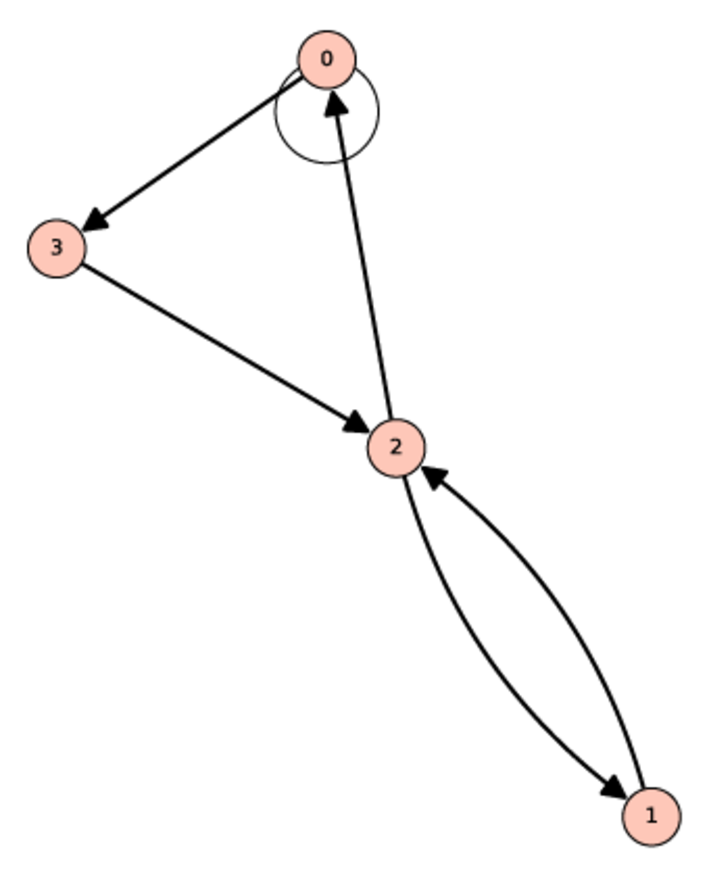
\includegraphics[width=\linewidth]{images/graph-6-2-1.pdf}}%
{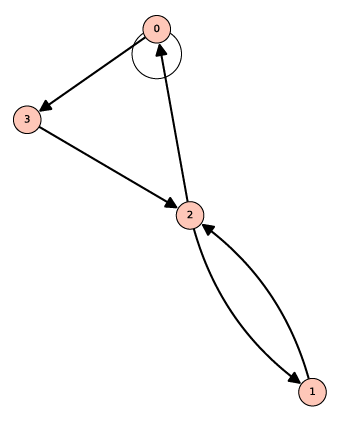
\includegraphics[width=\linewidth]{images/graph-6-2-1.png}}
\end{image}%
\tcblower
\end{figureptx}%
The actual location of the vertices in a digraph is immaterial. The actual location of vertices we choose is called an \terminology{embedding of a graph}\index{Embedding of a graph}. The main idea is to place the vertices in such a way that the graph is easy to read. After drawing a rough-draft graph of a relation, we may decide to relocate the vertices so that the final result will be neater. \hyperref[x:figure:fig-graph-6-2-1]{Figure~{\xreffont\ref{x:figure:fig-graph-6-2-1}}} could also be presented as in \hyperref[x:figure:fig-graph-6-2-2]{Figure~{\xreffont\ref{x:figure:fig-graph-6-2-2}}}.%
\begin{figureptx}{Alternate embedding of the previous directed graph}{x:figure:fig-graph-6-2-2}{}%
\begin{image}{0.2}{0.6}{0.2}%
\IfFileExists{images/graph-6-2-2.pdf}%
{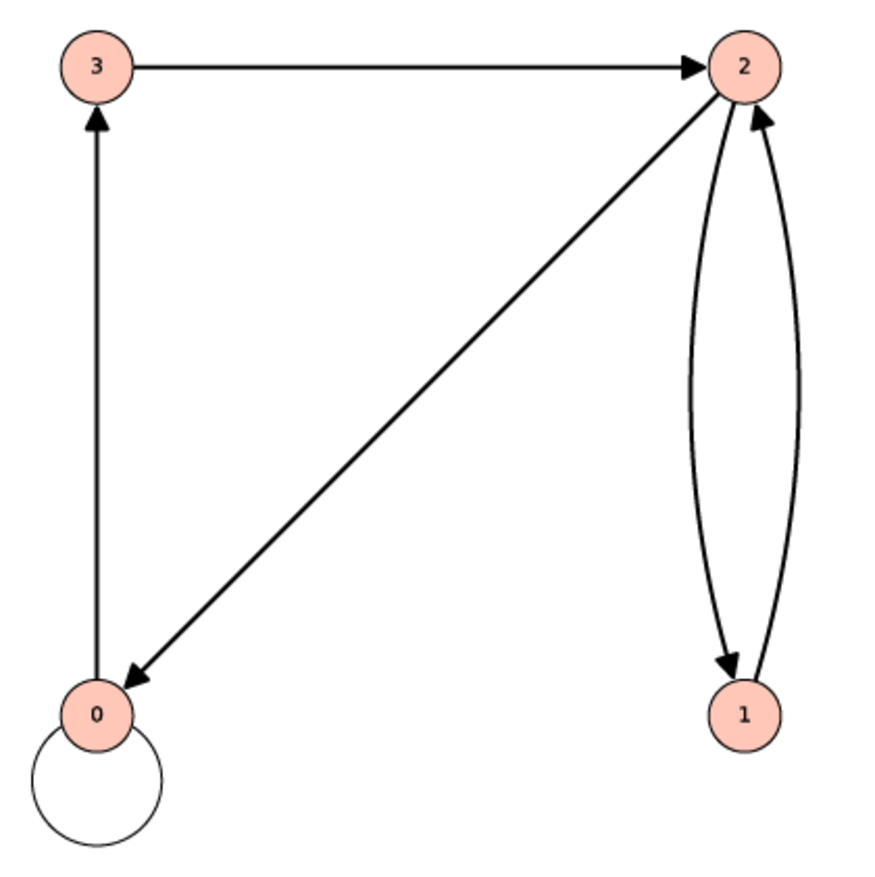
\includegraphics[width=\linewidth]{images/graph-6-2-2.pdf}}%
{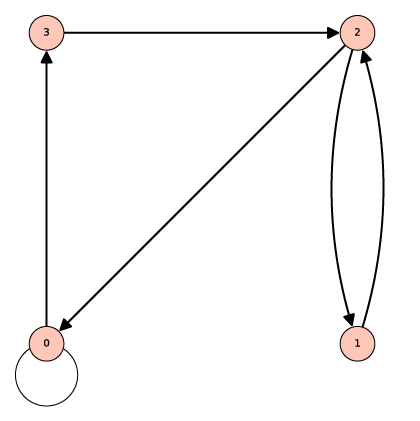
\includegraphics[width=\linewidth]{images/graph-6-2-2.png}}
\end{image}%
\tcblower
\end{figureptx}%
A vertex of a graph is also called a node, point, or a junction. An edge of a graph is also referred to as an arc, a line, or a branch. Do not be concerned if two graphs of a given relation look different as long as the connections between vertices are the same in the two graphs.%
\begin{example}{Another directed graph.}{x:example:ex-another-simple-graph}%
Consider the relation \(s\) whose digraph is \hyperref[x:figure:fig-graph-6-2-3]{Figure~{\xreffont\ref{x:figure:fig-graph-6-2-3}}}. What information does this give us? The graph tells us that \(s\) is a relation on \(A = \{1, 2, 3\}\) and that \(s = \{(1, 2), (2, 1), (1, 3), (3, 1), (2, 3), (3, 3)\}\).%
\begin{figureptx}{Digraph of the relation \(s\)}{x:figure:fig-graph-6-2-3}{}%
\begin{image}{0.2}{0.6}{0.2}%
\IfFileExists{images/graph-6-2-3.pdf}%
{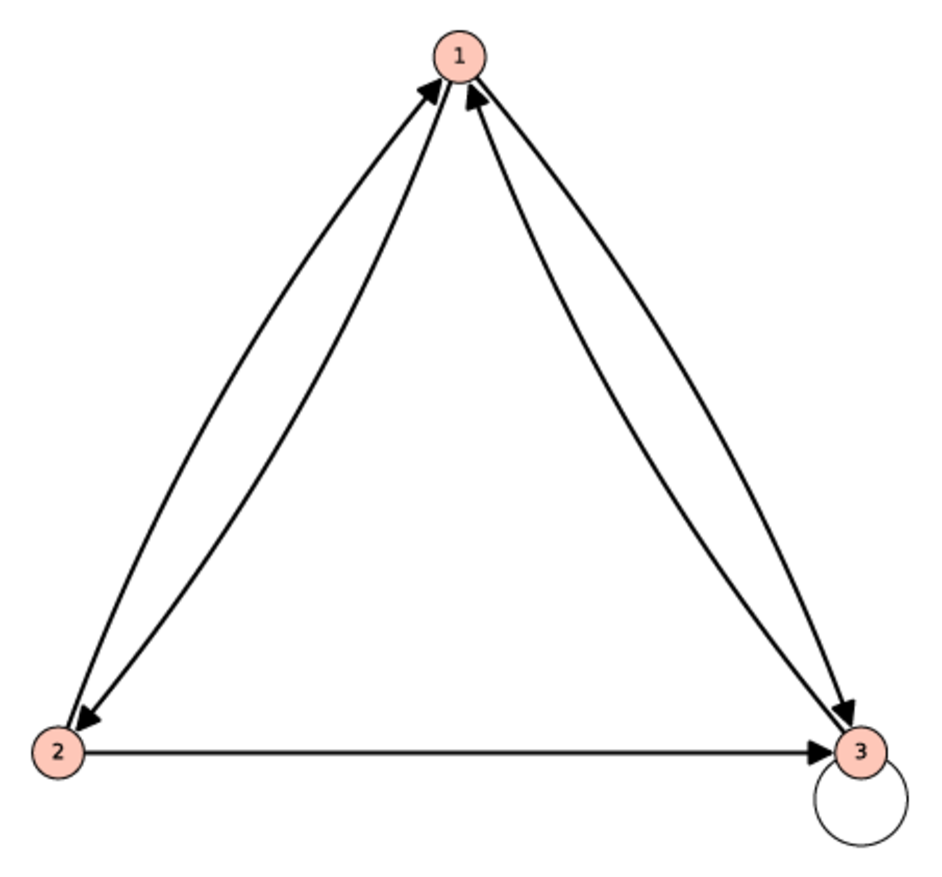
\includegraphics[width=\linewidth]{images/graph-6-2-3.pdf}}%
{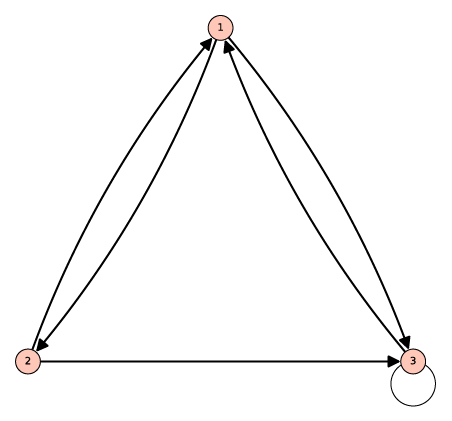
\includegraphics[width=\linewidth]{images/graph-6-2-3.png}}
\end{image}%
\tcblower
\end{figureptx}%
\end{example}
We will be building on the next example in the following section.%
\begin{example}{Ordering subsets of a two element universe.}{x:example:ex-subsets-2-ordering}%
Let \(B = \{1,2\}\), and let \(A = \mathcal{P}(B) = \{\emptyset, \{1\}, \{2\}, \{1,2\}\}\). Then \(\subseteq\) is a relation on \(A\) whose digraph is \hyperref[x:figure:fig-graph-6-2-subsets-2]{Figure~{\xreffont\ref{x:figure:fig-graph-6-2-subsets-2}}}.%
\begin{figureptx}{Graph for set containment on subsets of \(\{1,2\}\)}{x:figure:fig-graph-6-2-subsets-2}{}%
\begin{image}{0.2}{0.6}{0.2}%
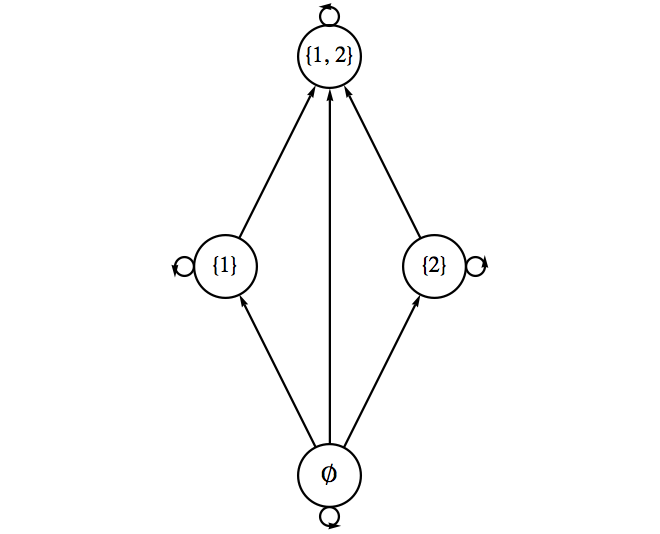
\includegraphics[width=\linewidth]{images/graph-6-2-subsets-2.png}
\end{image}%
\tcblower
\end{figureptx}%
We will see in the next section that since \(\subseteq\) has certain structural properties that describe ``partial orderings.'' We will be able to draw a much simpler type graph than this one, but for now the graph above serves our purposes.%
\end{example}
\end{subsectionptx}
%
%
\typeout{************************************************}
\typeout{Exercises 6.2.2 Exercises}
\typeout{************************************************}
%
\begin{exercises-subsection}{Exercises}{}{Exercises}{}{}{x:exercises:exercises-6-2}
\begin{divisionexercise}{1}{}{}{g:exercise:idm40464033360}%
Let \(A = \{1, 2, 3, 4\}\), and let \(r\) be the relation \(\leq\) on \(A\). Draw a digraph for \(r\).%
\end{divisionexercise}%
\begin{divisionexercise}{2}{}{}{g:exercise:idm40464027392}%
Let \(B = \{1,2, 3, 4, 6, 8, 12, 24\}\), and let \(s\) be the relation ``divides'' on \(B\). Draw a digraph for \(s\).%
\end{divisionexercise}%
\begin{divisionexercise}{3}{}{}{g:exercise:idm40464025632}%
Let \(A=\{1,2,3,4,5\}\). Define \(t\) on \(A\) by \(a t b\) if and only if \(b - a\) is even. Draw a digraph for \(t\).%
\end{divisionexercise}%
\begin{divisionexercise}{4}{}{}{g:exercise:idm40464017728}%
Let \(A\) be the set of strings of 0's and 1's of length 3 or less.%
\begin{enumerate}[label=(\alph*)]
\item{}Define the relation of \(d\) on \(A\) by \(x d y\) if \(x\) is contained within \(y\). For example, \(01 d 101\). Draw a digraph for this relation.%
\item{}Do the same for the relation \(p\) defined by \(x p y\) if \(x\) is a prefix of \(y\). For example, \(10 p 101\), but \(01 p 101\) is false.%
\end{enumerate}
%
\end{divisionexercise}%
\begin{divisionexercise}{5}{}{}{g:exercise:idm40464012912}%
Recall the relation in Exercise 5 of Section 6.1, \(\rho\) defined on the power set, \(\mathcal{P}(S)\), of a set \(S\). The definition was \((A,B) \in \rho\) iff \(A\cap  B = \emptyset\). Draw the digraph for \(\rho\) where \(S = \{a, b\}\).%
\end{divisionexercise}%
\begin{divisionexercise}{6}{}{}{g:exercise:idm40464009648}%
Let \(C= \{1,2, 3, 4, 6, 8, 12, 24\}\) and define \(t\) on \(C\) by \(a t b\) if and only if \(a\) and \(b\) share a common divisor greater than 1.  Draw a digraph for \(t\).%
\end{divisionexercise}%
\end{exercises-subsection}
\end{sectionptx}
%
%
\typeout{************************************************}
\typeout{Section 6.3 Properties of Relations}
\typeout{************************************************}
%
\begin{sectionptx}{Properties of Relations}{}{Properties of Relations}{}{}{x:section:s-properties-of-relations}
%
%
\typeout{************************************************}
\typeout{Subsection 6.3.1 Individual Properties}
\typeout{************************************************}
%
\begin{subsectionptx}{Individual Properties}{}{Individual Properties}{}{}{x:subsection:ss-individual-properties}
Consider the set \(B = \{1, 2, 3, 4, 6, 12, 36, 48\}\) and the relations ``divides'' and \(\leq \) on \(B\). We notice that these two relations on \(B\) have three properties in common:%
\par
%
\begin{itemize}[label=\textbullet]
\item{}Every element in \(B\) divides itself and is less than or equal to itself. This is called the reflexive property.%
\item{}If we search for two elements from \(B\) where the first divides the second and the second divides the first, then we are forced to choose the two numbers to be the same. In other words, no two \emph{different} numbers are related in both directions. The reader can verify that a similar fact is true for the relation \(\leq \) on \(B\). This is called the antisymmetric property.%
\item{}Next if we choose three values (not necessarily distinct) from \(B\) such that the first divides the second and the second divides the third, then we always find that the first number divides the third.  Again, the same is true if we replace ``divides'' with ``is less than or equal to.'' This is called the transitive property.%
\end{itemize}
%
\par
Relations that satisfy these properties are of special interest to us. Formal definitions of the properties follow.%
\begin{definition}{Reflexive Relation.}{x:definition:def-reflexive-relation}%
\index{Reflexive Relation}%
Let \(A\) be a set and let \(r\) be a relation on \(A\). Then \(r\) is \terminology{reflexive} if and only if \(a r a\) for all \(a \in A\).%
\end{definition}
\begin{definition}{Antisymmetric Relation.}{x:definition:def-antisymmetric-relation}%
\index{Antisymmetric Relation}%
Let \(A\) be a set and let \(r\) be a relation on \(A\).  Then \(r\) is \terminology{antisymmetric} if and only if whenever \(a r b\) and \(a \neq  b\) then \(b r a\) is false.%
\end{definition}
An equivalent condition for antisymmetry is that if \(a r b\) and  \(b r a\) then \(a = b\). You are encouraged to convince yourself that this is true.  This condition is often more convenient to prove than the definition, even though the definition is probably easier to understand.%
\par
A word of warning about antisymmetry: Students frequently find it difficult to understand this definition. Keep in mind that this term is defined through an ``If...then...'' statement. The question that you must ask is: Is it true that whenever there are elements \(a\) and \(b\) from \(A\) where \(a r b\) and \(a \neq  b\), it follows that \(b\) is not related to \(a\)? If so, then the relation  is antisymmetric.%
\par
Another way to determine whether a relation is antisymmetric is to examine (or imagine) its digraph. The relation is not antisymmetric if there exists a pair of vertices that are connected by edges in both directions.%
\begin{definition}{Transitive Relation.}{x:definition:def-transitive-relation}%
\index{Transitive Relation}%
Let \(A\) be a set and let \(r\) be a relation on \(A\). \(r\) is \terminology{transitive} if and only if whenever \(a r b\) and \(b r c\) then \(a r c\).%
\end{definition}
\end{subsectionptx}
%
%
\typeout{************************************************}
\typeout{Subsection 6.3.2 Partial Orderings}
\typeout{************************************************}
%
\begin{subsectionptx}{Partial Orderings}{}{Partial Orderings}{}{}{x:subsection:ss-partial-ordering}
Not all relations have all three of the properties discussed above, but those that do are a special type of relation.%
\begin{definition}{Partial Ordering.}{x:definition:partial-ordering}%
\index{Partial Ordering}%
\index{Poset}%
A relation on a set \(A\) that is reflexive, antisymmetric, and transitive is called a \terminology{partial ordering} on \(A\). A set on which there is a partial ordering relation defined is called a \terminology{partially ordered set}\index{Partially ordered set} or \terminology{poset}.%
\end{definition}
\begin{example}{Set Containment as a Partial Ordering.}{x:example:ex-subset-partial-ordering}%
Let \(A\) be a set. Then \(\mathcal{P}(A)\) together with the relation \(\subseteq\) (set containment) is a poset. To prove this we observe that the three properties hold, as discussed in Chapter 4.%
\par
%
\begin{itemize}[label=\textbullet]
\item{}Let \(B \in  \mathcal{P}(A)\). The fact that \(B \subseteq  B\) follows from the definition of subset. Hence, set containment is reflexive.%
\item{}Let \(B_1, B_2 \in \mathcal{P}(A)\) and assume that \(B_1\subseteq  B_2\) and \(B_1\neq  B_2\) . Could it be that \(B_2\subseteq  B_1\)? No. There must be some element \(a\in A\) such that \(a \notin B_1\), but \(a\in B_2\). This is exactly what we need to conclude that \(B_2\) is not contained in \(B_1\).  Hence, set containment is antisymmetric.%
\item{}Let \(B_1, B_2,B_3 \in \mathcal{P}(A)\) and assume that \(B_1 \subseteq  B_2\) and \(B_2 \subseteq  B_3\) . Does it follow that \(B_1 \subseteq B_3\) ? Yes, if \(a\in B_1\), then \(a\in B_2\) because \(B_1 \subseteq  B_2\). Now that we have \(a\in B_2\) and we have assumed \(B_2 \subseteq B_3\), we conclude that \(a\in B_3\).  Therefore, \(B_1\subseteq B_3\) and so set containment is transitive.%
\end{itemize}
%
\par
\hyperref[x:figure:fig-graph-6-2-subsets-2]{Figure~{\xreffont\ref{x:figure:fig-graph-6-2-subsets-2}}} is the graph for the ``set containment'' relation on the power set of \(\{1,2\}\).%
\end{example}
\index{Hasse Diagram}\index{Ordering Diagram}\hyperref[x:figure:fig-graph-6-2-subsets-2]{Figure~{\xreffont\ref{x:figure:fig-graph-6-2-subsets-2}}} is helpful insofar as it reminds us that each set is a subset of itself and shows us at a glance the relationship between the various subsets in \(\mathcal{P} (\{1,2\})\). However, when a relation is a partial ordering, we can streamline a graph like this one.  The streamlined form of a graph is called a \terminology{Hasse diagram} or \terminology{ordering diagram}.  A Hasse diagram takes into account the following facts.%
\par
%
\begin{itemize}[label=\textbullet]
\item{}By the reflexive property, each vertex must be related to itself, so the arrows from a vertex to itself (called ``self-loops'') are not drawn in a Hasse diagram. They are simply assumed.%
\item{}By the antisymmetry property, connections between two distinct elements in a directed graph can only go one way, if at all.  When there is a connection, we agree to always place the second element above the first (as we do above with the connection from \(\{1\}\) to \(\{1,2\}\)). For this reason, we can just draw a connection without an arrow, just a line.%
\item{}By the transitive property, if there are edges connecting one element up to a second element and the second element up to a third element, then there will be a direct connection from the first to the third. We see this in \hyperref[x:figure:fig-graph-6-2-subsets-2]{Figure~{\xreffont\ref{x:figure:fig-graph-6-2-subsets-2}}} with \(\emptyset\) connected to \(\{1\}\)\(\)and then \(\{1\}\) connected to \(\{1,2\}\). Notice the edge connecting \(\emptyset\) to \(\{1,2\}\).  Whenever we identify this situation, remove the connection from the first to the third in a Hasse diagram and simply observe that an upward path of any length implies that the lower element is related to the upper one.%
\end{itemize}
%
\par
Using these observations as a guide, we can draw a Hasse diagram for \(\subseteq\) on \(\{1,2\}\) as in \hyperref[x:figure:subsets_2_hasse]{Figure~{\xreffont\ref{x:figure:subsets_2_hasse}}}.%
\begin{figureptx}{Hasse diagram for set containment on subsets of \(\{1,2\}\)}{x:figure:subsets_2_hasse}{}%
\begin{image}{0.3}{0.4}{0.3}%
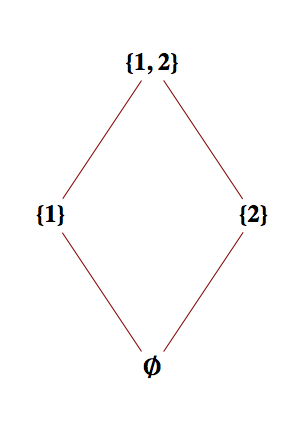
\includegraphics[width=\linewidth]{images/subsets_2_hasse.png}
\end{image}%
\tcblower
\end{figureptx}%
\begin{example}{Definition of a relation using a Hasse diagram.}{x:example:ex-def-by-hasse}%
Consider the partial ordering relation \(s\) whose Hasse diagram is \hyperref[x:figure:fig-pentagonal-hasse]{Figure~{\xreffont\ref{x:figure:fig-pentagonal-hasse}}}.%
\begin{figureptx}{Hasse diagram for the pentagonal poset}{x:figure:fig-pentagonal-hasse}{}%
\begin{image}{0.3}{0.4}{0.3}%
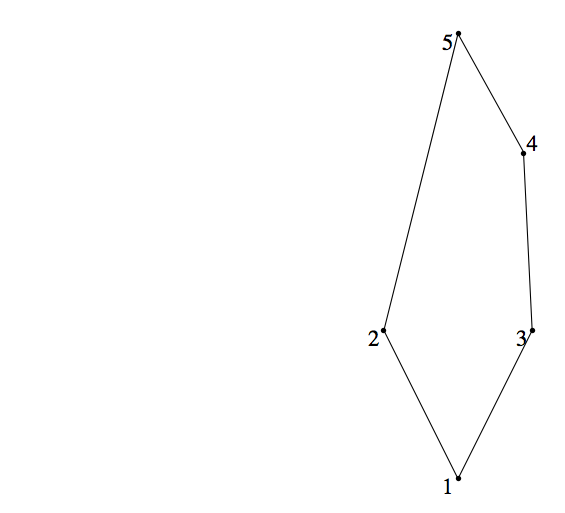
\includegraphics[width=\linewidth]{images/pentagonal-hasse.png}
\end{image}%
\tcblower
\end{figureptx}%
How do we read this diagram? What is \(A\)? What is \(s\)? What does the digraph of \(s\) look like? Certainly \(A = \{1,2,3,4,5\}\) and \(1 s 2\), \(3 s 4\), \(1 s 4\), \(1 s 5\), etc., Notice that \(1 s 5\) is implied by the fact that there is a path of length three upward from 1 to 5. This follows from the edges that are shown and the transitive property that is presumed in a poset.  Since \(1 s 3\) and \(3 s
4\), we know that \(1 s 4\). We then combine \(1 s 4\) with \(4 s 5\) to infer \(1 s 5\).  Without going into details why, here is a complete list of pairs defined by \(s\).%
\begin{equation*}
s = \{(1,1),(2,2),(3,3),(4,4),(5,5),(1,3),(1,4),(1,5),(1,2),(3,4),(3,5),(4,5),(2,5)\}
\end{equation*}
%
\par
A digraph for \(s\) is \hyperref[x:figure:fig-pentagonal-digraph]{Figure~{\xreffont\ref{x:figure:fig-pentagonal-digraph}}}. It is certainly more complicated to read and difficult to draw than the Hasse diagram.%
\begin{figureptx}{Digraph for the pentagonal poset}{x:figure:fig-pentagonal-digraph}{}%
\begin{image}{0.3}{0.4}{0.3}%
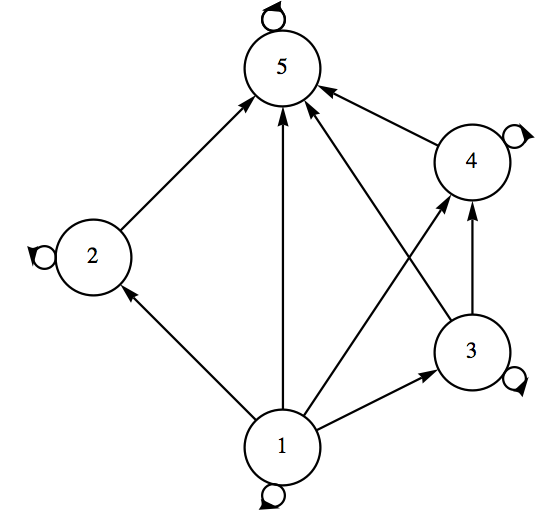
\includegraphics[width=\linewidth]{images/pentagonal-digraph.png}
\end{image}%
\tcblower
\end{figureptx}%
\end{example}
A classic example of a partial ordering relation is \(\leq \) on the real numbers, \(\mathbb{R}\). Indeed, when graphing partial ordering relations, it is natural to ``plot'' the elements from the given poset starting with the ``least'' element to the ``greatest'' and to use terms like ``least,'' ``greatest,'' etc. Because of this the reader should be forewarned that some texts use the symbol \(\leq\) for arbitrary partial orderings. This can be quite confusing for the novice, so we continue to use generic letters \(r\), \(s\), etc.%
\end{subsectionptx}
%
%
\typeout{************************************************}
\typeout{Subsection 6.3.3 Equivalence Relations}
\typeout{************************************************}
%
\begin{subsectionptx}{Equivalence Relations}{}{Equivalence Relations}{}{}{x:subsection:ss-equivalence-relations}
\index{Equivalence Relations}%
Another common property of relations is symmetry.%
\begin{definition}{Symmetric Relation.}{x:definition:def-symmetric-relation}%
\index{Symmetric Relation}%
Let \(r\) be a relation on a set \(A\). \(r\) is \terminology{symmetric} if and only if whenever \(a r b\), it follows that \(b r a\).%
\end{definition}
Consider the relation of equality defined on any set \(A\). Certainly \(a = b\) implies that \(b = a\) so equality is a symmetric relation on \(A\).%
\par
Surprisingly, equality is also an antisymmetric relation on \(A\). This is due to the fact that the condition that defines the antisymmetry property, \(a = b\) and \(a \neq  b\), is a contradiction. Remember, a conditional proposition is always true when the condition is false. So a relation can be both symmetric and antisymmetric on a set! Again recall that these terms are \emph{not} negatives of one other. That said, there are very few important relations other than equality that are both symmetric and antisymmetric.%
\begin{definition}{Equivalence Relation.}{x:definition:def-equivalence-relation}%
\index{Equivalence Relation}%
A relation \(r\) on a set \(A\) is called an equivalence relation if and only if it is reflexive, symmetric, and transitive.%
\end{definition}
The classic example of an equivalence relation is equality on a set \(A\). In fact, the term equivalence relation is used because those relations which satisfy the definition behave quite like the equality relation. Here is another important equivalence relation.%
\begin{example}{Equivalent Fractions.}{x:example:ex-fraction-equivalence}%
Let \(\mathbb{Z}^*\) be the set of nonzero integers. One of the most basic equivalence relations in mathematics is the relation \(q\) on \(\mathbb{Z}\times \mathbb{Z}^*\) defined by \((a, b) q(c, d)\) if and only if \(a d = b c\). We will leave it to the reader to, verify that \(q\) is indeed an equivalence relation. Be aware that since the elements of \(\mathbb{Z}\times \mathbb{Z}^*\) are ordered pairs, proving symmetry involves four numbers and transitivity involves six numbers. Two ordered pairs, \((a, b)\) and \((c, d)\), are related if the fractions \(\frac{a}{b}\) and \(\frac{c}{d}\) are numerically equal.%
\end{example}
Our next example involves the following fundamental relations on the set of integers.%
\begin{definition}{Congruence Modulo \(n\).}{x:definition:def-congruence-mod-n}%
\index{Congruence Modulo n}%
\label{g:notation:idm40463895856}%
\label{g:notation:idm40463894576}%
Let \(n\) be a positive integer, \(n\geq 2\).  We define \terminology{congruence modulo n} to be the relation \(\equiv_n\) defined on the integers by%
\begin{equation*}
a \equiv_n b \Leftrightarrow n \mid (a-b)
\end{equation*}
%
\end{definition}
We observe the following about congruence modulo \(n\):%
\par
%
\begin{itemize}[label=\textbullet]
\item{}This relation is reflexive, for if \(a \in  \mathbb{Z} \),  \(n \mid (a-a) \Rightarrow  a\equiv_n a \).%
\item{}This relation is symmetric. We can prove this through the following chain of implications.%
\begin{equation*}
\begin{split}
a \equiv_n b &\Rightarrow   n \mid (a-b)\\
& \Rightarrow \textrm{For  some } k \in \mathbb{Z}, a-b = n k \\
& \Rightarrow b-a = n (-k)\\
& \Rightarrow n \mid (b-a)\\
& \Rightarrow b \equiv_n a 
\end{split}\text{.}
\end{equation*}
%
\item{}Finally, this relation is transitive.  We leave it to the reader to prove that if \(a \equiv _n b \) and \(b\equiv _n c\), then \(a \equiv _n c\).%
\end{itemize}
%
\par
Frequently, you will see the equivalent notation \(a \equiv b (\textrm{mod } n)\) for congruence modulo \(n\).%
\begin{example}{Random Relations usually have no properties.}{x:example:ex-no-propery-relation}%
Consider the relation s described by the digraph in \hyperref[x:figure:fig-graph-6-3-5]{Figure~{\xreffont\ref{x:figure:fig-graph-6-3-5}}}. This was created by randomly selecting whether or not two elements from \(\{a,b,c\}\) were related or not. Convince yourself that the following are true:%
\par
%
\begin{itemize}[label=\textbullet]
\item{}This relation is not reflexive.%
\item{}It is not antisymmetric.%
\item{}Also, it is not symmetric.%
\item{}It is not transitive.%
\item{}Is \(s\) an equivalence relation or a partial ordering?%
\end{itemize}
%
\begin{figureptx}{Digraph of a random relation \(r\)}{x:figure:fig-graph-6-3-5}{}%
\begin{image}{0.25}{0.5}{0.25}%
\IfFileExists{images/graph-6-3-5.pdf}%
{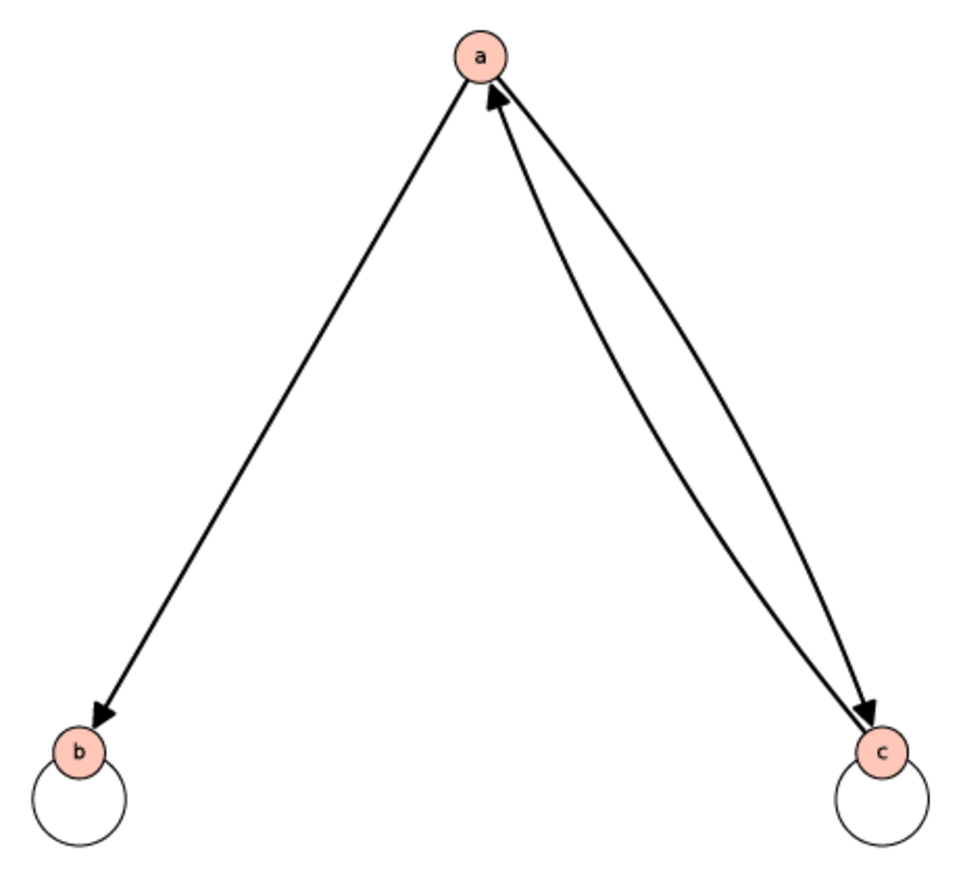
\includegraphics[width=\linewidth]{images/graph-6-3-5.pdf}}%
{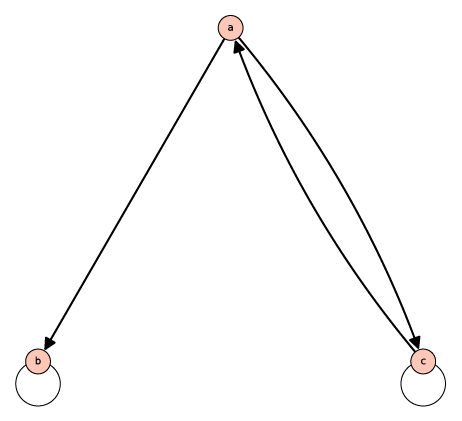
\includegraphics[width=\linewidth]{images/graph-6-3-5.png}}
\end{image}%
\tcblower
\end{figureptx}%
Not every random choice of a relation will be so totally negative, but as the underlying set increases, the likelihood any of the properties are true begins to vanish.%
\end{example}
\end{subsectionptx}
%
%
\typeout{************************************************}
\typeout{Exercises 6.3.4 Exercises}
\typeout{************************************************}
%
\begin{exercises-subsection}{Exercises}{}{Exercises}{}{}{x:exercises:exercises-6-3}
\begin{divisionexercise}{1}{}{}{g:exercise:idm40463874512}%
%
\begin{enumerate}[label=(\alph*)]
\item{}Let \(B = \{a, b\}\) and \(U = \mathcal{P}(B)\). Draw a Hasse diagram for \(\subseteq \) on \(U\).%
\item{}Let \(A = \{1,2, 3, 6\}\). Show that divides, \(\mid \), is a partial ordering on \(A\).%
\item{}Draw a Hasse diagram for divides on \(A\).%
\item{}Compare the graphs of parts a and c.%
\end{enumerate}
%
\end{divisionexercise}%
\begin{divisionexercise}{2}{}{}{g:exercise:idm40463865344}%
Repeat Exercise 1 with \(B = \{a, b, c\}\) and \(A = \{1, 2, 3, 5, 6, 10, 15, 30\}\).%
\par\smallskip%
\noindent\textbf{\blocktitlefont Hint}.\hypertarget{g:hint:idm40463862896}{}\quad{}\begin{sidebyside}{2}{0}{0}{0}%
\begin{sbspanel}{0.5}%
Here is a Hasse diagram for the part (a).%
\end{sbspanel}%
\begin{sbspanel}{0.5}%
\begin{figureptx}{}{x:figure:fig-subsets-3-hasse}{}%
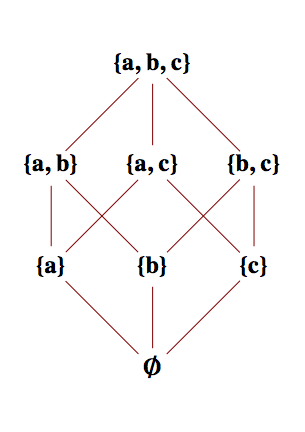
\includegraphics[width=\linewidth]{images/fig-subsets-3-hasse.png}
\tcblower
\end{figureptx}%
\end{sbspanel}%
\end{sidebyside}%
\end{divisionexercise}%
\begin{divisionexercise}{3}{}{}{g:exercise:idm40463860512}%
Consider the relations defined by the digraphs in \hyperref[x:figure:fig-exercises-6-digraphs]{Figure~{\xreffont\ref{x:figure:fig-exercises-6-digraphs}}}.%
\begin{enumerate}[label=(\alph*)]
\item{}Determine whether the given relations are reflexive, symmetric, antisymmetric, or transitive. Try to develop procedures for determining the validity of these properties from the graphs,%
\item{}Which of the graphs are of equivalence relations or of partial orderings?%
\end{enumerate}
%
\begin{figureptx}{Some digraphs of relations}{x:figure:fig-exercises-6-digraphs}{}%
\begin{image}{0}{1}{0}%
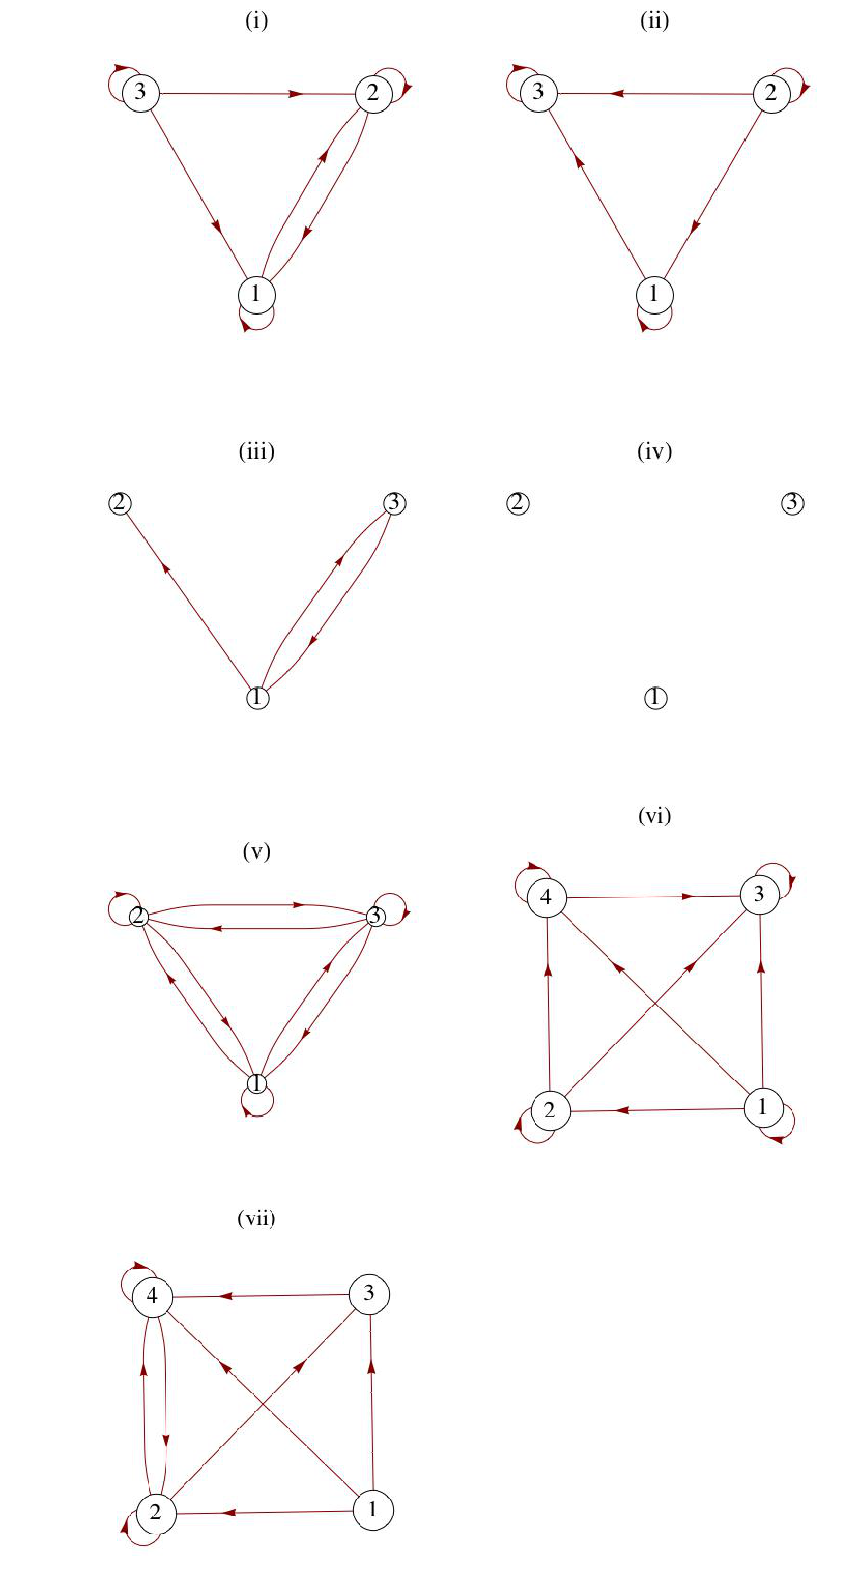
\includegraphics[width=\linewidth]{images/exercises-6-digraphs.png}
\end{image}%
\tcblower
\end{figureptx}%
\end{divisionexercise}%
\begin{divisionexercise}{4}{}{}{g:exercise:idm40463840912}%
Determine which of the following are equivalence relations and\slash{}or partial ordering relations for the given sets:%
\par
%
\begin{enumerate}[label=(\alph*)]
\item{}\(A = \{\textrm{ lines in the plane}\}\), and \(r\) defined by  \(x r y\) if and only if \(x\) is parallel to \(y\).  Assume every line is parallel to itself.%
\item{}\(A = \mathbb{R}\) and \(r\) defined by  \(x r y\) if and only if \(\lvert x -y \rvert \leq  7\).%
\end{enumerate}
%
\end{divisionexercise}%
\begin{divisionexercise}{5}{}{}{g:exercise:idm40463834736}%
Consider the  relation on \(\{1, 2, 3, 4, 5, 6\}\) defined by  \(r = \{(i,j):\enspace \lvert i - j\rvert  = 2\}\).%
\par
%
\begin{enumerate}[label=(\alph*)]
\item{}Is \(r\) reflexive?%
\item{}Is \(r\) symmetric?%
\item{}Is \(r\) transitive?%
\item{}Draw a graph of \(r\).%
\end{enumerate}
%
\end{divisionexercise}%
\begin{divisionexercise}{6}{}{}{g:exercise:idm40463822544}%
For the set of cities on a map, consider the relation \(x r y\) if and only if city \(x\) is connected by a road to city \(y\). A city is considered to be connected to itself, and two cities are connected even though there are cities on the road between them. Is this an equivalence relation or a partial ordering? Explain.%
\end{divisionexercise}%
\begin{divisionexercise}{7}{Equivalence Classes.}{}{x:exercise:equivalence-classes}%
Let \(A = \{0, 1, 2, 3\}\) and let%
\begin{equation*}
r = \{(0, 0), (1, 1), (2, 2), (3, 3), (1, 2),(2, 1), (3, 2), (2, 3), (3, 1), (1, 3)\}
\end{equation*}
%
\begin{enumerate}[label=(\alph*)]
\item{}Verify that \(r\) is an equivalence relation on \(A\).%
\item{}Let \(a \in A\) and define \(c(a) = \{b \in A \mid a rb\}\). \label{g:notation:idm40463814768} \(c(a)\) is called the \terminology{equivalence class of \(a\) under \(r\)}\index{Equivalence Class}. Find \(c(a)\) for each element \(a \in A\).%
\item{}Show that \(\{c(a) \mid  a \in A\}\) forms a partition of \(A\) for this set \(A\).%
\item{}Let \(r\) be an equivalence relation on an arbitrary set \(A\). Prove that the set of all equivalence classes under \(r\) constitutes a partition of \(A\).%
\end{enumerate}
%
\end{divisionexercise}%
\begin{divisionexercise}{8}{}{}{g:exercise:idm40463792384}%
Define \(r\) on the power set of \(\{1, 2, 3\}\) by \(A r B \Leftrightarrow  \lvert A \rvert = \lvert B \rvert \). Prove that \(r\) is an equivalence relation. What are the equivalence classes under \(r\)?%
\end{divisionexercise}%
\begin{divisionexercise}{9}{}{}{g:exercise:idm40463791776}%
Consider the following relations on \(\mathbb{Z}_8= \{0, 1, . . . , 7\}\). Which are equivalence relations? For the equivalence relations, list the equivalence classes.%
\par
%
\begin{enumerate}[label=(\alph*)]
\item{}\(a r b\) iff the English spellings of \(a\) and \(b\) begin with the same letter.%
\item{}\(a s b\) iff \(a - b\) is a positive integer.%
\item{}\(a t b\) iff \(a-b\) is an even integer.%
\end{enumerate}
%
\end{divisionexercise}%
\begin{divisionexercise}{10}{}{}{g:exercise:idm40463780064}%
Building on \hyperlink{x:exercise:equivalence-classes}{Exercise~{\xreffont 6.3.4.7}}:%
\par
%
\begin{enumerate}[label=(\alph*)]
\item{}Prove that congruence modulo \(m\) is transitive.%
\item{}What are the equivalence classes under congruence modulo 2?%
\item{}What are the equivalence classes under congruence modulo 10?%
\end{enumerate}
%
\end{divisionexercise}%
\begin{divisionexercise}{11}{}{}{g:exercise:idm40463776448}%
In this exercise, we prove that implication is a partial ordering. Let \(A\) be any set of propositions.%
\par
%
\begin{enumerate}[label=(\alph*)]
\item{}Verify that \(q \to  q\) is a tautology, thereby showing that \(\Rightarrow\) is a reflexive relation on \(A\).%
\item{}Prove that \(\Rightarrow\) is antisymmetric on \(A\). Note: we do not use = when speaking of propositions, but rather equivalence, \(\Leftrightarrow\).%
\item{}Prove that \(\Rightarrow\) is transitive on \(A\).%
\item{}Given that \(q_i\) is the proposition \(n < i\) on \(\mathbb{N}\), draw the Hasse diagram for the relation \(\Rightarrow\) on \(\{q_1, q_2, q_3,\ldots \}\).%
\end{enumerate}
%
\end{divisionexercise}%
\begin{divisionexercise}{12}{}{}{x:exercise:exercise-6-3-12}%
Let \(S = \{1,2,3,4,5,6,7\}\) be a poset \((S, \leq )\) with the Hasse diagram shown below. Another relation \(r \subseteq  S\times S\) is defined as follows: \((x, y) \in  r\) if and only if there exists \(z \in S\) such that \(z < x\) and \(z < y\) in the poset \((S, \leq )\).%
\par
%
\begin{enumerate}[label=(\alph*)]
\item{}Prove that \(r\) is reflexive.%
\item{}Prove that \(r\) is symmetric.%
\item{}A compatible with respect to relation \(r\) is any subset \(Q\) of set \(S\) such that \(x \in  Q \textrm{ and } y \in Q \Rightarrow  (x, y) \in r\). A compatible \(g\) is a maximal compatible if \(Q\) is not a proper subset of another compatible. Give all maximal compatibles with respect to relation \(r\) defined above.%
\item{}Discuss a characterization of the set of maximal compatibles for relation \(r\) when \((S, \leq )\) is a general finite poset. What conditions, if any, on a general finite poset \((S, \leq )\) will make \(r\) an equivalence relation?%
\end{enumerate}
%
\begin{figureptx}{Hasse diagram for \(r\) in exercise 12.}{x:figure:fig-exercise-6-12}{}%
\begin{image}{0}{1}{0}%
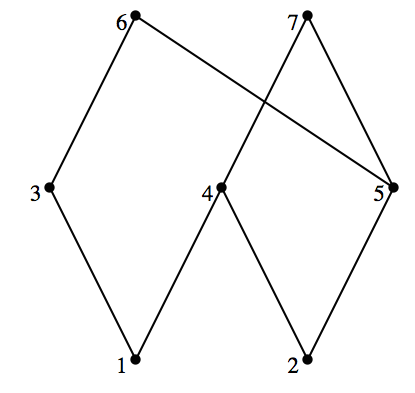
\includegraphics[width=\linewidth]{images/exercise-6-12.png}
\end{image}%
\tcblower
\end{figureptx}%
\end{divisionexercise}%
\end{exercises-subsection}
\end{sectionptx}
%
%
\typeout{************************************************}
\typeout{Section 6.4 Matrices of Relations}
\typeout{************************************************}
%
\begin{sectionptx}{Matrices of Relations}{}{Matrices of Relations}{}{}{x:section:s-matrices-of-relations}
\begin{introduction}{}%
We have discussed two of the many possible ways of representing a relation, namely as a digraph or as a set of ordered pairs. In this section we will discuss the representation of relations by matrices.%
\end{introduction}%
%
%
\typeout{************************************************}
\typeout{Subsection 6.4.1 Representing a Relation with a Matrix}
\typeout{************************************************}
%
\begin{subsectionptx}{Representing a Relation with a Matrix}{}{Representing a Relation with a Matrix}{}{}{g:subsection:idm40463746832}
\begin{definition}{Adjacency Matrix.}{x:definition:def-adjacency-matrix}%
\index{Adjacency Matrix}%
Let \(A = \{a_1,a_2,\ldots , a_m\}\) and \(B= \{b_1,b_2,\ldots , b_n\}\) be finite sets of cardinality \(m\) and \(n\), respectively. Let \(r\) be a relation from \(A\) into \(B\). Then \(r\) can be represented by the \(m\times n\) matrix \(R\) defined by%
\begin{equation*}
R_{ij}= \left\{
\begin{array}{cc}
1 & \textrm{   if } a_i r b_j \\
0 & \textrm{   otherwise}     \\
\end{array}\right.
\end{equation*}
\(R\) is called the \terminology{adjacency matrix} (or the relation matrix) of \(r\).%
\end{definition}
\begin{example}{A simple example.}{x:example:ex-first-6-4}%
Let \(A = \{2, 5, 6\}\) and let \(r\) be the relation \(\{(2, 2), (2, 5), (5, 6), (6, 6)\}\) on \(A\). Since \(r\) is a relation from \(A\) into the same set \(A\) (the \(B\) of the definition), we have \(a_1= 2\), \(a_2=5\), and \(a_3=6\), while \(b_1= 2\), \(b_2=5\), and \(b_3=6\). Next, since%
\par
%
\begin{itemize}[label=\textbullet]
\item{}\(2 r 2\), we have \(R_{11}= 1\)%
\item{}\(2 r 5\), we have \(R_{12}= 1\)%
\item{}\(5 r 6\), we have \(R_{23}= 1\)%
\item{}\(6 r 6\), we have \(R_{33}= 1\)%
\end{itemize}
%
\par
All other entries of \(R\) are zero, so%
\begin{equation*}
R =\left(
\begin{array}{ccc}
1 & 1 & 0 \\
0 & 0 & 1 \\
0 & 0 & 1 \\
\end{array}
\right)
\end{equation*}
%
\end{example}
\end{subsectionptx}
%
%
\typeout{************************************************}
\typeout{Subsection 6.4.2 Composition as Matrix Multiplication}
\typeout{************************************************}
%
\begin{subsectionptx}{Composition as Matrix Multiplication}{}{Composition as Matrix Multiplication}{}{}{g:subsection:idm40463726320}
From the definition of \(r\) and of composition, we note that%
\begin{equation*}
r^2 = \{(2, 2), (2, 5), (2, 6), (5, 6), (6, 6)\}
\end{equation*}
The adjacency matrix of \(r^2\) is%
\begin{equation*}
R^2 =\left(
\begin{array}{ccc}
1 & 1 & 1 \\
0 & 0 & 1 \\
0 & 0 & 1 \\
\end{array}
\right)\text{.}
\end{equation*}
%
\par
We do not write \(R^2\) only for notational purposes. In fact, \(R^2\) can be obtained from the matrix product \(R R\); however, we must use a slightly different form of arithmetic.%
\begin{definition}{Boolean Arithmetic.}{x:definition:def-boolean-arithmetic}%
\index{Boolean Arithmetic}%
Boolean arithmetic is the arithmetic defined on \(\{0,1\}\) using Boolean addition and Boolean multiplication, defined by%
\begin{tableptx}{\textbf{}}{g:table:idm40463720304}{}%
\centering
{\tabularfont%
\begin{tabular}{lll}
\(0 + 0 = 0\)&\(0+1 = 1 + 0=1\)&\(1 + 1 = 1\)\tabularnewline[0pt]
\(0\cdot 0=0\)&\(0 \cdot  1 = 1 \cdot  0 = 0\)&\(1 \cdot  1 = 1\)
\end{tabular}
}%
\end{tableptx}%
\end{definition}
Notice that from Chapter 3, this is the ``arithmetic of logic,'' where \(+\) replaces ``or'' and \(\cdot\) replaces ``and.''%
\begin{example}{Composition by Multiplication.}{x:example:ex-composition-matrices}%
Suppose that \(R=\left(
\begin{array}{cccc}
0 & 1 & 0 & 0 \\
1 & 0 & 1 & 0 \\
0 & 1 & 0 & 1 \\
0 & 0 & 1 & 0 \\
\end{array}
\right)\)  and  \(S=\left(
\begin{array}{cccc}
0 & 1 & 1 & 1 \\
0 & 0 & 1 & 1 \\
0 & 0 & 0 & 1 \\
0 & 0 & 0 & 0 \\
\end{array}
\right)\). Then using Boolean arithmetic, \(R S =\left(
\begin{array}{cccc}
0 & 0 & 1 & 1 \\
0 & 1 & 1 & 1 \\
0 & 0 & 1 & 1 \\
0 & 0 & 0 & 1 \\
\end{array}
\right)\)  and \(S R=\left(
\begin{array}{cccc}
1 & 1 & 1 & 1 \\
0 & 1 & 1 & 1 \\
0 & 0 & 1 & 0 \\
0 & 0 & 0 & 0 \\
\end{array}
\right)\).%
\end{example}
\begin{theorem}{Composition is Matrix Multiplication.}{}{x:theorem:theorem-composition-is-multiplication}%
Let \(A_1\), \(A_2\), and \(A_3\) be finite sets where \(r_1\) is a relation from \(A_1\) into \(A_2\) and \(r_2\) is a relation from \(A_2\) into \(A_3\). If \(R_1\) and \(R_2\) are the adjacency matrices of \(r_1\) and \(r_2\), respectively, then the product \(R_1R_2\) using Boolean arithmetic is the adjacency matrix of the composition \(r_1r_2\).%
\end{theorem}
Remark: A convenient help in constructing the adjacency matrix of a relation from a set \(A\) into a set \(B\) is to write the elements from \(A\) in a column preceding the first column of the adjacency matrix, and the elements of \(B\) in a row above the first row. Initially, \(R\) in \hyperref[x:example:ex-first-6-4]{Example~2} would be%
\begin{equation*}
\begin{array}{cc}
& 
\begin{array}{ccc}
2 & 5 & 6 \\
\end{array}
\\
\begin{array}{c}
2 \\
5 \\
6 \\
\end{array}
& \left(
\begin{array}{ccc}
&   &   \\
&   &   \\
&   &   \\
\end{array}
\right) \\
\end{array}
\end{equation*}
To fill in the matrix, \(R_{ij}\) is 1 if and only if \(\left(a_i,b_j\right) \in r\). So that, since the pair \((2, 5) \in r\), the entry of \(R\) corresponding to the row labeled 2 and the column labeled 5 in the matrix is a 1.%
\begin{example}{Relations and Information.}{x:example:ex-relations-information}%
This final example gives an insight into how relational data base programs can systematically answer questions pertaining to large masses of information. Matrices \(R\) (on the left) and \(S\) (on the right) define the relations \(r\) and \(s\) where \(a r b\) if software \(a\) can be run with operating system \(b\), and \(b s c\) if operating system \(b\) can run on computer \(c\).%
\begin{equation*}
\begin{array}{cc}
\begin{array}{cc}
& 
\begin{array}{cccc}
\text{OS1} & \text{OS2} & \text{OS3} & \text{OS4} 
\end{array} \\ 
\begin{array}{c}
\text{P1} \\
\text{P2} \\
\text{P3} \\
\text{P4}
\end{array}
&
\left(
\begin{array}{cccc}
1  &  0  &  1  &  0  \\
1  &  1  & 0 & 0 \\
0 & 0 & 0 &  1  \\
0 & 0 &  1  &  1
\end{array}
\right) 
\end{array}
\begin{array}{cc}
& 
\begin{array}{ccc}
\text{C1} & \text{C2} & \text{C3}
\end{array} \\
\begin{array}{c}
\text{OS1} \\
\text{OS2} \\
\text{OS3} \\
\text{OS4} \\
\end{array}
& \left(
\begin{array}{ccc}
1  &  1  & 0 \\
0 &  1  & 0 \\
0 & 0 &  1  \\
0 &  1  &  1 
\end{array}
\right)
\end{array}
\end{array}
\end{equation*}
Although the relation between the software and computers is not implicit from the data given, we can easily compute this information. The matrix of \(rs\) is \(RS\), which is%
\begin{equation*}
\begin{array}{cc}
& 
\begin{array}{ccc}
\text{C1} & \text{C2} & \text{C3}
\end{array}
\\
\begin{array}{c}
\text{P1} \\
\text{P2} \\
\text{P3} \\
\text{P4}
\end{array}
& \left(
\begin{array}{ccc}
1  &  1  & 1 \\
1 &  1  & 0 \\
0 & 1 &  1  \\
0 &  1  &  1 
\end{array}
\right) 
\end{array}
\end{equation*}
This matrix tells us at a glance which software will run on the computers listed. In this case, all software will run on all computers with the exception of program P2, which will not run on the computer C3, and programs P3 and P4, which will not run on the computer C1.%
\end{example}
\end{subsectionptx}
%
%
\typeout{************************************************}
\typeout{Exercises 6.4.3 Exercises}
\typeout{************************************************}
%
\begin{exercises-subsection}{Exercises}{}{Exercises}{}{}{x:exercises:exercises-6-4}
\begin{divisionexercise}{1}{}{}{g:exercise:idm40463686688}%
Let \(A_1 = \{1,2, 3, 4\}\), \(A_2 = \{4, 5, 6\}\), and \(A_3 = \{6, 7, 8\}\). Let \(r_1\) be the relation from \(A_1\) into \(A_2\) defined by \(r_1 = \{(x, y)  \mid  y - x = 2\}\), and let \(r_2\) be the relation from \(A_2\) into \(A_3\) defined by \(r_2 = \{(x, y) \mid  y - x = 1\}\).%
\par
%
\begin{enumerate}[label=(\alph*)]
\item{}Determine the adjacency matrices of \(r_1\) and \(r_2\).%
\item{}Use the definition of composition to find \(r_1r_2\).%
\item{}Verify the result in part b by finding the product of the adjacency matrices of \(r_1\) and \(r_2\).%
\end{enumerate}
%
\end{divisionexercise}%
\begin{divisionexercise}{2}{}{}{g:exercise:idm40463672816}%
%
\begin{enumerate}[label=(\alph*)]
\item{}Determine the adjacency matrix of each relation given via the digraphs in Exercise 3 of Section 6.3.%
\item{}Using the matrices found in part (a) above, find \(r^2\) of each relation in Exercise 3 of Section 6.3.%
\item{}Find the digraph of \(r^2\) directly from the given digraph and compare your results with those of part (b).%
\end{enumerate}
%
\end{divisionexercise}%
\begin{divisionexercise}{3}{}{}{g:exercise:idm40463669664}%
Suppose that the matrices in \hyperref[x:example:ex-composition-matrices]{Example~{\xreffont\ref{x:example:ex-composition-matrices}}} are relations on \(\{1, 2, 3, 4\}\). What relations do \(R\) and \(S\) describe?%
\end{divisionexercise}%
\begin{divisionexercise}{4}{}{}{g:exercise:idm40463663408}%
Let \(D\) be the set of weekdays, Monday through Friday, let \(W\) be a set of employees \(\{1, 2, 3\}\) of a tutoring center, and let \(V\) be a set of computer languages for which tutoring is offered,  \(\{A(PL), B(asic), C(++), J(ava), L(isp), P(ython)\}\). We define \(s\) (schedule) from \(D\) into \(W\) by \(d s w\) if \(w\) is scheduled to work on day \(d\). We also define \(r\) from \(W\) into \(V\) by \(w r l\) if \(w\) can tutor students in language \(l\). If \(s\) and \(r\) are defined by matrices%
\par
%
\begin{equation*}
S = 
\begin{array}{cc}
& 
\begin{array}{ccc}
1 & 2 & 3 \\
\end{array}
\\
\begin{array}{c}
M \\
T \\
W \\
R \\
F \\
\end{array}
& 
\left(
\begin{array}{ccc}
1 & 0 & 1 \\
0 & 1 & 1 \\
1 & 0 & 1 \\
0 & 1 & 0 \\
1 & 1 & 0 \\
\end{array}
\right) \\
\end{array}
\textrm{ and }R=
\begin{array}{cc}
& 
\begin{array}{cccccc}
A & B & C & J & L & P \\
\end{array}
\\
\begin{array}{c}
1 \\
2 \\
3 \\
\end{array}
& \left(
\begin{array}{cccccc}
0 & 1 & 1 & 0 & 0 & 1 \\
1 & 1 & 0 & 1 & 0 & 1 \\
0 & 1 & 0 & 0 & 1 & 1 \\
\end{array}
\right) \\
\end{array}
\end{equation*}
%
\par
%
\begin{enumerate}[label=(\alph*)]
\item{}compute \(S R\) using Boolean arithmetic and give an interpretation of the relation it defines, and%
\item{}compute \(S R\) using regular arithmetic and give an interpretation of what the result describes.%
\end{enumerate}
%
\end{divisionexercise}%
\begin{divisionexercise}{5}{}{}{g:exercise:idm40463651792}%
How many different reflexive, symmetric relations are there on a set with three elements?%
\par\smallskip%
\noindent\textbf{\blocktitlefont Hint}.\hypertarget{g:hint:idm40463650128}{}\quad{}Consider the possible matrices.%
\end{divisionexercise}%
\begin{divisionexercise}{6}{}{}{g:exercise:idm40463648688}%
Let \(A = \{a, b, c, d\}\).  Let \(r\) be the relation on \(A\) with adjacency matrix \(\begin{array}{cc}
& 
\begin{array}{cccc}
a & b & c & d \\
\end{array}
\\
\begin{array}{c}
a \\
b \\
c \\
d \\
\end{array}
& \left(
\begin{array}{cccc}
1 & 0 & 0 & 0 \\
0 & 1 & 0 & 0 \\
1 & 1 & 1 & 0 \\
0 & 1 & 0 & 1 \\
\end{array}
\right) \\
\end{array}\)%
\par
%
\begin{enumerate}[label=(\alph*)]
\item{}Explain why \(r\) is a partial ordering on \(A\).%
\item{}Draw its Hasse diagram.%
\end{enumerate}
%
\end{divisionexercise}%
\begin{divisionexercise}{7}{}{}{g:exercise:idm40463644016}%
Define relations \(p\) and \(q\) on \(\{1, 2, 3, 4\}\) by \(p = \{(a, b) \mid \lvert a-b\rvert=1\}\) and \(q=\{(a,b) \mid a-b \textrm{ is even}\}\).%
\par
%
\begin{enumerate}[label=(\alph*)]
\item{}Represent \(p\) and \(q\) as both graphs and matrices.%
\item{}Determine \(p q\), \(p^2\), and \(q^2\); and represent them clearly in any way.%
\end{enumerate}
%
\end{divisionexercise}%
\begin{divisionexercise}{8}{}{}{g:exercise:idm40463633216}%
%
\begin{enumerate}[label=(\alph*)]
\item{}Prove that if \(r\) is a transitive relation on a set \(A\), then \(r^2 \subseteq  r\).%
\item{}Find an example of a transitive relation for which \(r^2\neq r\).%
\end{enumerate}
%
\end{divisionexercise}%
\begin{divisionexercise}{9}{}{}{g:exercise:idm40463629696}%
We define \(\leq\) on the set of all \(n\times n\) relation matrices by the rule that if \(R\) and \(S\) are any two \(n\times n\) relation matrices, \(R \leq  S\) if and only if \(R_{ij} \leq S_{ij}\) for all \(1 \leq  i, j \leq  n\).%
\par
%
\begin{enumerate}[label=(\alph*)]
\item{}Prove that \(\leq\) is a partial ordering on all \(n\times n\) relation matrices.%
\item{}Prove that \(R \leq  S  \Rightarrow   R^2\leq S^2\) , but the converse is not true.%
\item{}If \(R\) and \(S\) are matrices of equivalence relations and \(R \leq  S\), how are the equivalence classes defined by \(R\) related to the equivalence classes defined by \(S\)?%
\end{enumerate}
%
\end{divisionexercise}%
\end{exercises-subsection}
\end{sectionptx}
%
%
\typeout{************************************************}
\typeout{Section 6.5 Closure Operations on Relations}
\typeout{************************************************}
%
\begin{sectionptx}{Closure Operations on Relations}{}{Closure Operations on Relations}{}{}{x:section:s-closure-operations-on-relations}
\begin{introduction}{}%
In Section 6.1, we studied relations and one important operation on relations, namely composition. This operation enables us to generate new relations from previously known relations. In Section 6.3, we discussed some key properties of relations. We now wish to consider the situation of constructing a new relation \(r^+\) from an existing relation \(r\) where, first, \(r^+\) contains \(r\) and, second, \(r^{+ }\) satisfies the transitive property.%
\end{introduction}%
%
%
\typeout{************************************************}
\typeout{Subsection 6.5.1 Transitive Closure}
\typeout{************************************************}
%
\begin{subsectionptx}{Transitive Closure}{}{Transitive Closure}{}{}{g:subsection:idm40463602432}
Consider a telephone network in which the main office \(a\) is connected to, and can communicate to, individuals \(b\) and \(c\).  Both \(b\) and \(c\) can communicate to another person, \(d\); however, the main office cannot communicate with \(d\). Assume communication is only one way, as indicated. This situation can be described by the relation \(r = \{(a, b), (a, c), (b, d), (c, d)\}\). We would like to change the system so that the main office \(a\) can communicate with person \(d\) and still maintain the previous system. We, of course, want the most economical system.%
\par
This can be rephrased as follows; Find the smallest relation \(r^{+ }\) which contains \(r\) as a subset and which is transitive; \(r^+ =\{(a, b), (a, c), (b, d), (c, d), (a, d)\}\).%
\begin{definition}{Transitive Closure.}{x:definition:def-transitive-closure}%
\index{Transitive Closure}%
\label{g:notation:idm40463592384}%
Let \(A\) be a set and \(r\) be a relation on \(A\). The transitive closure of \(r\), denoted by \(r^+\), is the smallest transitive relation that contains \(r\) as a subset.%
\end{definition}
Let \(A = \{1, 2, 3, 4\}\), and let \(\mathcal{S} = \{(1, 2), (2, 3), (3, 4)\}\) be a relation on \(A\). This relation is called the successor relation on \(A\) since each element is related to its successor. How do we compute \(\mathcal{S}^+\)?  By inspection we note that \((1, 3)\) must be in \(\mathcal{S}^+\) . Let's analyze why. This is so because \((1,2) \in \mathcal{S}\) and \((2, 3) \in \mathcal{S}\), and the transitive property forces \((1,3)\) to be in \(\mathcal{S}^+\).%
\par
In general, it follows that if \((a, b) \in \mathcal{S}\) and \((b, c) \in S,\) then \((a, c) \in \mathcal{S}^+ \). This condition is exactly the membership requirement for the pair \((a, c)\) to be in the composition \(\mathcal{S}\mathcal{S} = \mathcal{S}^2\). So every element in \(\mathcal{S}^2\) must be an element in \(\mathcal{S}^+\) . So we now know that, \(\mathcal{S}^+\) contains at least \(\mathcal{S} \cup  \mathcal{S}^2\) . In particular, for this example, since \(\mathcal{S} = \{(1, 2), (2, 3), (3, 4)\}\) and \(\mathcal{S}^2 = \{(1, 3), (2, 4)\}\), we have%
\begin{equation*}
\mathcal{S} \cup  \mathcal{S}^2 =\{(1, 2), (2, 3), (3, 4), (1, 3), (2, 4)\}
\end{equation*}
%
\par
Is the relation \(\mathcal{S} \cup  \mathcal{S}^2\) transitive? Again, by inspection, \((1, 4)\) is not an element of \(\mathcal{S} \cup  \mathcal{S}^2\), but  \((1,3) \in \mathcal{S}^2\) and \((3, 4) \in \mathcal{S}\). Therefore, the composition \(\mathcal{S}^2 \mathcal{S} = \mathcal{S}^3\) produces \((1, 4)\), and it must be an element of \(\mathcal{S}^+\) since \((1,3)\) and \((3, 4)\) are required to be in \(\mathcal{S}^+\).  This shows that \(\mathcal{S}^3 \subseteq  \mathcal{S}^+\). This process must be continued until the resulting relation is transitive. If \(A\) is finite, as is true in this example, the transitive closure will be obtained in a finite number of steps. For this example,%
\begin{equation*}
\mathcal{S}^+ =\mathcal{S}\cup \mathcal{S} ^2\cup  \mathcal{S} ^3=\{(1, 2), (2, 3), (3, 4),(1, 3),(2, 4),(1,4)\}
\end{equation*}
%
\begin{theorem}{Transitive Closure on a Finite Set.}{}{x:theorem:theorem-transitive-closure-formula}%
If \(r\) is a relation on a set \(A\) and \(\lvert A \rvert = n\), then the transitive closure of \(r\) is the union of the first \(n\) powers of r.  That is,%
\begin{equation*}
r^+ = r \cup  r^2 \cup  r ^3 \cup \cdots  \cup  r^n\text{.}
\end{equation*}
%
\end{theorem}
Let's now consider the matrix analogue of the transitive closure.%
\par
Consider the relation%
\begin{equation*}
r = \{(1, 4), (2, 1), (2, 2), (2, 3),(3, 2), (4, 3), (4, 5), (5, 1)\}
\end{equation*}
on the set \(A = \{1,2, 3, 4, 5\}\). The matrix of \(r\) is%
\begin{equation*}
R=\left(
\begin{array}{ccccc}
0 & 0 & 0 & 1 & 0 \\
1 & 1 & 1 & 0 & 0 \\
0 & 1 & 0 & 0 & 0 \\
0 & 0 & 1 & 0 & 1 \\
1 & 0 & 0 & 0 & 0 \\
\end{array}
\right)
\end{equation*}
%
\par
Recall that \(r^2, r^3, \ldots\)  can be determined through computing the matrix powers \(R^2, R^3, \ldots\).  For our example,%
\begin{tableptx}{\textbf{}}{g:table:idm40491755616}{}%
\centering
{\tabularfont%
\begin{tabular}{ll}
\(R^2=\left(
\begin{array}{ccccc}
0 & 0 & 1 & 0 & 1 \\
1 & 1 & 1 & 1 & 0 \\
1 & 1 & 1 & 0 & 0 \\
1 & 1 & 0 & 0 & 0 \\
0 & 0 & 0 & 1 & 0 \\
\end{array}
\right)\)&\(R^3=\left(
\begin{array}{ccccc}
1 & 1 & 0 & 0 & 0 \\
1 & 1 & 1 & 1 & 1 \\
1 & 1 & 1 & 1 & 0 \\
1 & 1 & 1 & 1 & 0 \\
0 & 0 & 1 & 0 & 1 \\
\end{array}
\right)\)\tabularnewline[0pt]
\(R^4=\left(
\begin{array}{ccccc}
1 & 1 & 1 & 1 & 0 \\
1 & 1 & 1 & 1 & 1 \\
1 & 1 & 1 & 1 & 1 \\
1 & 1 & 1 & 1 & 1 \\
1 & 1 & 0 & 0 & 0 \\
\end{array}
\right)\)&\(R^5=\left(
\begin{array}{ccccc}
1 & 1 & 1 & 1 & 1 \\
1 & 1 & 1 & 1 & 1 \\
1 & 1 & 1 & 1 & 1 \\
1 & 1 & 1 & 1 & 1 \\
1 & 1 & 1 & 1 & 0 \\
\end{array}
\right)\)
\end{tabular}
}%
\end{tableptx}%
How do we relate \(\underset{i=1}{\overset{5}{\cup }}r^i\) to the powers of \(R\)?%
\begin{theorem}{Matrix of a Transitive Closure.}{}{x:theorem:theorem-matrix-transitive-closure}%
Let \(r\) be a relation on a finite set and \(R\) its matrix.  Let \(R^+\) be the matrix of \(r^+\), the transitive closure of \(r\).  Then \(R^+ = R + R^2 + \cdots + R^n\), using Boolean arithmetic.%
\end{theorem}
Using this theorem, we find \(R^+\) is the \(5\times 5\) matrix consisting of all \(1's\), thus, \(r^+\) is all of \(A \times A\).%
\end{subsectionptx}
%
%
\typeout{************************************************}
\typeout{Subsection 6.5.2 Algorithms for computing transitive closure}
\typeout{************************************************}
%
\begin{subsectionptx}{Algorithms for computing transitive closure}{}{Algorithms for computing transitive closure}{}{}{g:subsection:idm40491556768}
Let \(r\) be a relation on the set \(\{1, 2, \dots , n\}\) with relation matrix \(R\). The matrix of the transitive closure \(R^+\), can be computed by the equation \(R^+ = R + R ^2 + \cdots  + R^n\). By using ordinary polynomial evaluation methods, you can compute \(R^+\) with \(n -1\) matrix multiplications:%
\begin{equation*}
R^+ = R(I + R(I +( \cdots  R(I+ R) \cdots )))
\end{equation*}
%
\par
For example, if \(n = 3\), \(R^+ = R(I + R(I + R))\).%
\par
We can make use of the fact that if \(T\) is a relation matrix, \(T + T = T\) due to the fact that \(1 + 1 = 1\) in Boolean arithmetic. Let \(S_k = R + R^2 + \cdots  + R^k\). Then%
\par
%
\begin{equation*}
\begin{split}
R &= S_1\\
S_1(I+S_1)&=R(I+R)=R+R^2 = S_2 \\
S_2(I+S_2)&=(R+R^2)(I+R+R^2) \\
&=(R+R^2)+(R^2+R^3)+(R^3+R^4) \\
&=R+R^2+R^3+R^4 = S_4 
\end{split}\text{.}
\end{equation*}
%
\par
Similarly,%
\begin{equation*}
S_4(I+S_4)=S_8
\end{equation*}
and by induction we can prove%
\begin{equation*}
S_{2^k}(I+S_{2^k})=S_{2^{k+1}}
\end{equation*}
%
\par
Notice how each matrix multiplication doubles the number of terms that have been added to the sum that you currently have computed. In algorithmic form, we can compute \(R^+\) as follows.%
\begin{algorithm}{Transitive Closure Algorithm.}{}{x:algorithm:alg-trans-closure}%
Let \(R\) be a relation matrix and let \(R^+\) be its transitive closure matrix, which is to be computed as matrix \(T\)%
\begin{listingptx}{}{g:listing:idm40492101520}{}%
\begin{program}{none}
1.0. S = R
2.0  T= S*(I+S)
3.0 While T != S
		3.1 S = T
		3.2 T= S*(I+S) // using Boolean arithmetic
4.0 Return T
\end{program}
\tcblower
\end{listingptx}%
\end{algorithm}
\begin{note}{}{g:note:idm40491764944}%
%
\begin{itemize}[label=\textbullet]
\item{}Often the higher-powered terms in \(S_n\) do not contribute anything to \(R^+\). When the condition \(T = S\) becomes true in Step 3, this is an indication that no higher-powered terms are needed.%
\item{}To compute \(R^+\) using this algorithm, you need to perform no more than \(\lceil \log_2 n \rceil\) matrix multiplications, where \(\lceil x \rceil\) is the least integer that is greater than or equal to \(x\). For example, if \(r\) is a relation on 25 elements, no more than \(\lceil \log_2 25 \rceil = 5\) matrix multiplications are needed.%
\end{itemize}
%
\end{note}
A second algorithm, Warshall's Algorithm, reduces computation time to the time that it takes to multiply two square matrices with the same order as the relation matrix in question.%
\begin{algorithm}{Warshall's Algorithm.}{}{x:algorithm:alg-warshall}%
Let \(R\) be an \(n \times n\) relation matrix and let \(R^+\) be its transitive closure matrix, which is to be computed as matrix \(T\) using Boolean arithmetic%
\begin{listingptx}{}{g:listing:idm40469157904}{}%
\begin{program}{none}
1.0 T = R
2.0 for k = 1 to n:
     for i = 1 to n:
      for j = 1 to n:
        T[i,j]= T[i,j] + T[i,k] * T[k,j]
3.0 Return T
\end{program}
\tcblower
\end{listingptx}%
\end{algorithm}
\end{subsectionptx}
%
%
\typeout{************************************************}
\typeout{Exercises 6.5.3 Exercises}
\typeout{************************************************}
%
\begin{exercises-subsection}{Exercises}{}{Exercises}{}{}{x:exercises:exercises-6-5}
\begin{divisionexercise}{1}{}{}{g:exercise:idm40469236720}%
Let \(A =\{0, 1, 2, 3, 4\}\) and \(\mathcal{S}=\{(0, 1), (1, 3), (2, 3), (3, 4), (4, 1)\}\). Compute \(\mathcal{S}^+\) using the matrix representation of \(\mathcal{S}\). Verify your results by checking against the result obtained directly from the definition of transitive closure.%
\end{divisionexercise}%
\begin{divisionexercise}{2}{}{}{g:exercise:idm40469223296}%
Let \(A=\{1,2,3,4,6,12\}\) and \(t=\{(a,b)\mid b/a \textrm{ is a prime number}\}\). Determine \(t^+\) by any means.  Represent your answer as a matrix.%
\end{divisionexercise}%
\begin{divisionexercise}{3}{}{}{g:exercise:idm40469263136}%
%
\begin{enumerate}[label=(\alph*)]
\item{}Draw digraphs of the relations \(\mathcal{S}\), \(\mathcal{S}^2\), \(\mathcal{S}^3\) , and \(\mathcal{S}^+\)  where \(\mathcal{S}\) is defined in the first exercise above.%
\item{}Verify that in terms of the graph of \(\mathcal{S}\), \(a \mathcal{S}^+ b\) if and only if \(b\) is reachable from \(a\) along a path of any finite nonzero length.%
\end{enumerate}
%
\end{divisionexercise}%
\begin{divisionexercise}{4}{}{}{g:exercise:idm40469297968}%
Let \(r\) be the relation represented by the following digraph.%
\par
%
\begin{enumerate}[label=(\alph*)]
\item{}Find \(r^+\) using the definition based on order pairs.%
\item{}Determine the digraph of \(r^+\) directly from the digraph of \(r\).%
\item{}Verify your result in part (b) by computing the digraph from your result in part (a).%
\end{enumerate}
%
\begin{figureptx}{Digraph of \(r\) in exercise 4.}{g:figure:idm40469442224}{}%
\begin{image}{0.05}{0.9}{0.05}%
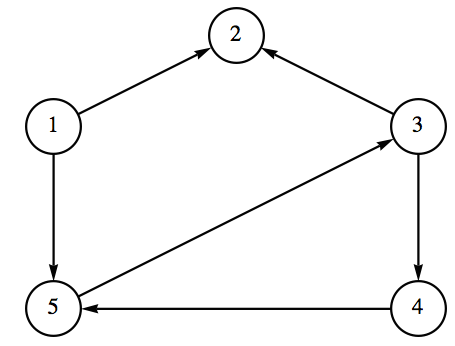
\includegraphics[width=\linewidth]{images/fig-exercise-6-5-4.png}
\end{image}%
\tcblower
\end{figureptx}%
\end{divisionexercise}%
\begin{divisionexercise}{5}{}{}{g:exercise:idm40469385488}%
%
\begin{enumerate}[label=(\alph*)]
\item{}Define reflexive closure and symmetric closure by imitating the definition of transitive closure.%
\item{}Use your definitions to compute the reflexive and symmetric closures of examples in the text.%
\item{}What are the transitive reflexive closures of these examples?%
\item{}Convince yourself that the reflexive closure of the relation \(<\) on the set of positive integers \(\mathbb{P}\) is \(\leq\).%
\end{enumerate}
%
\end{divisionexercise}%
\begin{divisionexercise}{6}{}{}{g:exercise:idm40469434240}%
What common relations on \(\mathbb{Z}\) are the transitive closures of the following relations?%
\par
%
\begin{enumerate}[label=(\alph*)]
\item{}\(a S b\) if and only if \(a + 1 = b\).%
\item{}\(a R b\) if and only if \(| a - b | = 2\).%
\end{enumerate}
%
\end{divisionexercise}%
\begin{divisionexercise}{7}{}{}{g:exercise:idm40468652096}%
%
\begin{enumerate}[label=(\alph*)]
\item{}Let \(A\) be any set and \(r\) a relation on \(A\), prove that \(\left(r^+\right)^+=r^+\).%
\item{}Is the transitive closure of a symmetric relation always both symmetric and reflexive? Explain.%
\end{enumerate}
%
\end{divisionexercise}%
\begin{divisionexercise}{8}{}{}{g:exercise:idm40468733264}%
The definition of the \hyperref[x:definition:def-transitive-closure]{Transitive Closure} of \(r\) refers to the ``smallest transitive relation that contains \(r\) as a subset.''  Show that the intersection of all transitive relations on \(A\) containing \(r\) is a transitive relation containing \(r\) and is precisely \(r^+\).%
\end{divisionexercise}%
\end{exercises-subsection}
\end{sectionptx}
\end{chapterptx}
%
%
\typeout{************************************************}
\typeout{Chapter 7 Functions}
\typeout{************************************************}
%
\begin{chapterptx}{Functions}{}{Functions}{}{}{x:chapter:chapter_7}
\begin{introduction}{}%
\begin{poem}%
\poemTitle{countably infinite}
\begin{stanza}
\poemlineleft{A \terminology{countably infinite} set}
\poemlineleft{Is as simple as things like this get.}
\poemlineleft{Just start counting at 1,}
\poemlineleft{Then continue—it's fun!}
\poemlineleft{I'll check back when you're done, so don't sweat.}
\end{stanza}
\poemauthorleft{Chris Doyle, The Omnificent English Dictionary In Limerick Form}
\end{poem}
In this chapter we will consider some basic concepts of the relations that are called functions. A large variety of mathematical ideas and applications can be more completely understood when expressed through the function concept.%
\end{introduction}%
%
%
\typeout{************************************************}
\typeout{Section 7.1 Definition and Notation}
\typeout{************************************************}
%
\begin{sectionptx}{Definition and Notation}{}{Definition and Notation}{}{}{x:section:s-function-def-notation}
%
%
\typeout{************************************************}
\typeout{Subsection 7.1.1 Fundamentals}
\typeout{************************************************}
%
\begin{subsectionptx}{Fundamentals}{}{Fundamentals}{}{}{x:subsection:ss-fundamentals-functions}
\begin{definition}{Function.}{x:definition:def-function}%
\index{Function}%
\label{g:notation:idm40468085040}%
A function from a set \(A\) into a set \(B\) is a relation from \(A\) into \(B\) such that each element of \(A\) is related to exactly one element of the set \(B\). The set \(A\) is called the \terminology{domain} of the function and the set \(B\) is called the \terminology{codomain}.%
\end{definition}
The reader should note that a function \(f\) is a relation from \(A\) into \(B\) with two important restrictions:%
\par
%
\begin{itemize}[label=\textbullet]
\item{}Each element in the set \(A\), the domain of \(f\), must be related to some element of \(B\), the codomain.%
\item{}The phrase ``is related to exactly one element of the set \(B\)'' means that if \((a, b)\in f\) and \((a, c)\in f\), then \(b = c\).%
\end{itemize}
%
\begin{example}{A function as a list of ordered pairs.}{x:example:ex-function-1}%
Let \(A = \{-2, -1,0, 1, 2\}\) and \(B = \{0, 1, 2, 3, 4\}\), and if \(s = \{(-2, 4), (-1, 1), (0, 0), (1, 1), (2, 4)\}\), then \(s\) is a function from \(A\) into \(B\).%
\end{example}
\begin{example}{A function as a set of ordered pairs in set-builder notation.}{x:example:ex-function-2}%
Let \(\mathbb{R}\) be the real numbers. Then \(L = \{(x, 3x) \mid x \in \mathbb{R}\}\) is a function from \(\mathbb{R}\) into \(\mathbb{R}\), or, more simply, \(L\) is a function on \(\mathbb{R}\).%
\end{example}
It is customary to use a different system of notation for functions than the one we used for relations. If \(f\) is a function from the set  \(A\) into the set \(B\), we will write \(f:A \rightarrow B\).%
\par
The reader is probably more familiar with the notation for describing functions that is used in basic algebra or calculus courses. For example, \(y =\frac{1}{x}\) or \(f(x) =\frac{1}{x}\) both define the function \(\left\{\left.\left(x,\frac{1}{x}\right)\right| x\in \mathbb{R}, x\neq
0\right\}\). Here the domain was assumed to be those elements of \(\mathbb{R}\) whose substitutions for \(x\) make sense, the nonzero real numbers, and the codomain was assumed to be \(\mathbb{R}\). In most cases, we will make a point of listing the domain and codomain in addition to describing what the function does in order to define a function.%
\par
The terms \terminology{mapping}, \terminology{map}, and \terminology{transformation} are also used for functions.%
\begin{definition}{The Set of Functions Between Two Sets.}{x:definition:def-set-of-functions}%
\index{Set of Functions Between Two Sets}%
\index{Functions Between Two Sets!Set of}%
\label{g:notation:idm40492059200}%
Given two sets,  \(A\) and \(B\), the set of all functions from \(A\) into \(B\) is denoted  \(B^A\).%
\end{definition}
The notation used for sets of functions makes sense in light of \hyperlink{x:exercise:exercise-counting-functions}{Exercise~5}.%
\par
One way to imagine a function and what it does is to think of it as a machine. The machine could be mechanical, electronic, hydraulic, or abstract. Imagine that the machine only accepts certain objects as raw materials or input. The possible raw materials make up the domain. Given some input, the machine produces a finished product that depends on the input. The possible finished products that we imagine could come out of this process make up the codomain.%
\begin{example}{A definition based on images.}{x:example:ex-non-pair-description}%
We can define a function based on specifying the codomain element to which each domain element is related.   For example, \(f: \mathbb{R} \rightarrow \mathbb{R}\) defined by \(f(x) = x^2\) is an alternate description of \(f= \left\{\left.\left(x,
x ^2\right)\right|x \in  \mathbb{R}\right\}\).%
\end{example}
\begin{definition}{Image of an element under a function.}{x:definition:def-image-of-an-element}%
\index{Image of an Element.}%
\label{g:notation:idm40469357120}%
Let \(f:A \rightarrow  B\), read ``Let \(f\) be a function from the set \(A\) into the set \(B\).'' If \(a \in  A\), then \(f(a)\) is used to denote that element of \(B\) to which \(a\) is related. \(f(a)\) is called the \terminology{image} of \(a\), or, more precisely, the image of \(a\) under \(f\). We write \(f(a) = b\) to indicate that the image of \(a\) is \(b\).%
\end{definition}
In \hyperref[x:example:ex-non-pair-description]{Example~{\xreffont\ref{x:example:ex-non-pair-description}}}, the image of 2 under \(f\) is 4; that is, \(f(2) = 4\). In \hyperref[x:example:ex-function-1]{Example~{\xreffont\ref{x:example:ex-function-1}}}, the image of \(-1\) under \(s\) is 1; that is, \(s(-1) = 1\).%
\begin{definition}{Range of a Function.}{x:definition:def-range-of-function}%
\index{Range of a Function.}%
\label{g:notation:idm40468281424}%
The range of a function is the set of images of its domain. If \(f:X \rightarrow Y\), then the range of \(f\) is denoted \(f(X)\), and%
\begin{equation*}
f(X) = \{f(a) \mid a \in X\} = \{b \in Y \mid  \exists a \in X\textrm{ such that } f(a) = b\}\text{.}
\end{equation*}
%
\end{definition}
Note that the range of a function is a subset of its codomain. \(f(X)\) is also read as ``the image of the set \(X\) under the function \(f\)'' or simply ``the image of \(f\).''%
\par
In \hyperref[x:example:ex-function-1]{Example~{\xreffont\ref{x:example:ex-function-1}}}, \(s(A)= \{0, 1, 4\}\). Notice that 2 and 3 are not images of any element of \(A\). In addition, note that both 1 and 4 are related to more than one element of the domain: \(s(1) = s(-1) = 1\) and \(s(2) = s(-2) = 4\). This does not violate the definition of a function. Go back and read the definition if this isn't clear to you.%
\par
In \hyperref[x:example:ex-function-2]{Example~{\xreffont\ref{x:example:ex-function-2}}}, the range of \(L\) is equal to its codomain, \(\mathbb{R}\). If \(b\) is any real number, we can demonstrate that it belongs to \(L(\mathbb{R})\) by finding a real number \(x\) for which \(L(x) = b\). By the definition of \(L\), \(L(x) = 3x\), which leads us to the equation \(3x = b\). This equation always has a solution, \(\frac{b}{3}\); thus \(L(\mathbb{R}) = \mathbb{R}\).%
\par
The formula that we used to describe the image of a real number under \(L\), \(L(x) = 3x\), is preferred over the set notation for \(L\) due to its brevity. Any time a function can be described with a rule or formula, we will use this form of description. In \hyperref[x:example:ex-function-1]{Example~{\xreffont\ref{x:example:ex-function-1}}}, the image of each element of \(A\) is its square. To describe that fact, we write \(s(a) = a^2\) (\(a \in  A\)), or \(S:A \rightarrow  B\) defined by \(S(a) = a^2\).%
\par
There are many ways that a function can be described. Many factors, such as the complexity of the function, dictate its representation.%
\begin{example}{Data as a function.}{x:example:ex-data-function}%
Suppose a survey of 1,000 persons is done asking how many hours of television each watches per day. Consider the function \(W:
\{0,1,\ldots , 24\} \rightarrow  \{0,1,2,\ldots ,1000\}\) defined by%
\begin{equation*}
W(t) = \textrm{the number of persons who gave a response of } t \textrm{ hours}
\end{equation*}
This function will probably have no formula such as the ones for \(s\) and \(L\) above.%
\end{example}
\begin{example}{Conditional definition of a function.}{x:example:ex-conditional-function}%
Consider the function \(m:\mathbb{P} \rightarrow  \mathbb{Q}\) defined by the set%
\begin{equation*}
m = \{(1, 1), (2, 1/2), (3, 9), (4, 1/4), (5, 25), . . . \} 
\end{equation*}
No simple single formula could describe \(m\), but if we assume that the pattern given continues, we can write%
\begin{equation*}
m(x) =\left\{
\begin{array}{cc}
x^2 &  \textrm{if } x \textrm{ is odd} \\
1/x & \textrm{if } x \textrm{ is even} \\
\end{array}
\right.
\end{equation*}
%
\end{example}
\end{subsectionptx}
%
%
\typeout{************************************************}
\typeout{Subsection 7.1.2 Functions of Two Variables}
\typeout{************************************************}
%
\begin{subsectionptx}{Functions of Two Variables}{}{Functions of Two Variables}{}{}{x:subsection:ss-two-variables}
\index{Functions!Of two Variables}%
If the domain of a function is the Cartesian product of two sets, then our notation and terminology changes slightly. For example, consider the function \(C:\mathbb{N} \times \mathbb{N}\rightarrow \mathbb{N}\) defined by \(C\left(\left(n_1,n_2\right)\right)=n_1^2+n_2^2- n_1n_2+10\).  For this function, we would drop one set of parentheses and write \(C(4, 2) = 22\), not \(C((4, 2)) = 22\). We call \(C\) a function of two variables. From one point of view, this function is no different from any others that we have seen. The elements of the domain happen to be slightly more complicated. On the other hand, we can look at the individual components of the ordered pairs as being separate. If we interpret \(C\) as giving us the cost of producing quantities of two products, we can imagine varying \(n_1\) while \(n_2\) is fixed, or vice versa.%
\end{subsectionptx}
%
%
\typeout{************************************************}
\typeout{Subsection 7.1.3 SageMath Note}
\typeout{************************************************}
%
\begin{subsectionptx}{SageMath Note}{}{SageMath Note}{}{}{x:subsection:ss-sage-note-functions}
\index{SageMath Note!Functions}%
There are several ways to define a function in Sage. The simplest way to implement \(f\) is as follows.%
\begin{sageinput}
f(x)=x^2
f
\end{sageinput}
\begin{sageoutput}
x |--> x^2
\end{sageoutput}
\begin{sageinput}
[f(4),f(1.2)]
\end{sageinput}
\begin{sageoutput}
[16, 1.44000000000000]
\end{sageoutput}
Sage is built upon the programming language Python, which is a \emph{strongly typed language} and so you can't evaluate expressions such as \mono{f(\textquotesingle{}Hello\textquotesingle{})}. However a function such as \(f\), as defined above, will accept any type of number, so a bit more work is needed to restrict the inputs of \(f\) to the integers.%
\par
A second way to define a function in Sage is based on Python syntax.%
\begin{sageinput}
def fa(x):
    return x^2
    
#end of definition - now we test it:
[fa(2),fa(1.2)]
\end{sageinput}
\begin{sageoutput}
[16, 1.44000000000000]
\end{sageoutput}
\end{subsectionptx}
%
%
\typeout{************************************************}
\typeout{Subsection 7.1.4 Non-Functions}
\typeout{************************************************}
%
\begin{subsectionptx}{Non-Functions}{}{Non-Functions}{}{}{x:subsection:ss-non-functions}
We close this section with two examples of relations that are not functions.%
\begin{example}{A non-function.}{x:example:ex-nonfunction1}%
Let \(A = B = \{1, 2, 3\}\) and let \(f= \{(1, 2), (2, 3)\}\). Here \(f\) is not a function from \(A\) into \(B\) since \(f\) does not act on, or ``use,'' all elements of \(A\).%
\end{example}
\begin{example}{Another non-function.}{x:example:ex-nonfunction2}%
Let \(A = B = \{1,2, 3\}\) and let \(g = \{(1, 2), (2, 3), (2, 1),(3, 2)\}\). We note that \(g\) acts on all of \(A\).  However, \(g\) is still not a function since \((2, 3) \in  g\) and \((2, 1) \in  g\) and the condition on each domain being related to exactly one element of the codomain is violated.%
\end{example}
\end{subsectionptx}
%
%
\typeout{************************************************}
\typeout{Exercises 7.1.5 Exercises}
\typeout{************************************************}
%
\begin{exercises-subsection}{Exercises}{}{Exercises}{}{}{x:exercises:exercises-7-1}
\begin{divisionexercise}{1}{}{}{x:exercise:exercise-7-1-1}%
Let \(A = \{1, 2, 3, 4\}\) and \(B = \{a, b, c, d\}\). Determine which of the following are functions. Explain.%
\par
%
\begin{enumerate}[label=(\alph*)]
\item{}\(f \subseteq  A \times  B\), where \(f = \{(1, a), (2, b), (3, c), (4, d)\}\).%
\item{}\(g\subseteq A\times B\), where \(g = \{(1, a), (2, a), (3,b), (4,d)\}\).%
\item{}\(h \subseteq A \times  B\), where \(h = \{(1, a), (2, b), (3, c)\}\).%
\item{}\(k \subseteq A\times  B\), where \(k = \{(1, a), (2, b), (2, c), (3, a), (4, a)\}\).%
\item{}\(L\subseteq A\times A\), where \(L = \{(1, 1), (2, 1), (3, 1), (4, 1)\}\).%
\end{enumerate}
%
\end{divisionexercise}%
\begin{divisionexercise}{2}{}{}{g:exercise:idm40492188560}%
Find the ranges of the following functions on \(\mathbb{Z}\):%
\par
%
\begin{enumerate}[label=(\alph*)]
\item{}\(g = \{(x, 4x +1)|x \in  \mathbb{Z}\}\).%
\item{}\(h(x) = \textrm{the least integer that is greater than or equal to } \sqrt{|x|}\).%
\item{}\(P(x) = x + 10\).%
\end{enumerate}
%
\end{divisionexercise}%
\begin{divisionexercise}{3}{}{}{g:exercise:idm40492184656}%
Find the ranges of each of the relations that are functions in Exercise 1.%
\end{divisionexercise}%
\begin{divisionexercise}{4}{}{}{x:exercise:exercise-characteristic-function}%
Let \(A\) be a set and let \(S\) be any subset of \(A\). Let \(\chi_S: A\to \{0,1\}\) be defined by%
\begin{equation*}
\chi_S(x)= \left\{
\begin{array}{cc}
1 & \textrm{if } x\in S \\
0 & \textrm{if } x\notin S \\
\end{array}
\right.
\end{equation*}
%
\par
The function \(\chi_S\) is called the \terminology{characteristic function}\index{Characteristic function} of \(S\).%
\par
%
\begin{enumerate}[label=(\alph*)]
\item{}If \(A = \{a, b, c\}\) and \(S = \{a, b\}\), list the elements of \(\chi_S\) .%
\item{}If \(A = \{a, b, c, d, e\}\) and \(S = \{a, c, e\}\), list the elements of \(\chi_S\).%
\item{}If \(A = \{a, b, c\}\), what are \(\chi_{\emptyset}\) and \(\chi_A\)?%
\end{enumerate}
%
\end{divisionexercise}%
\begin{divisionexercise}{5}{}{}{x:exercise:exercise-counting-functions}%
If \(A\) and \(B\) are finite sets, how many different functions are there from \(A\) into \(B\)?%
\end{divisionexercise}%
\begin{divisionexercise}{6}{}{}{g:exercise:idm40492053312}%
Let \(U\) be a set with subsets \(A\) and \(B\).%
\par
%
\begin{enumerate}[label=(\alph*)]
\item{}Show that \(g:U\to \{0,1\}\) defined by \(g(a)=\min \left(C_A(a),C_B(a)\right)\) is the characteristic function of \(A\cap B\).%
\item{}What characteristic function is \(h:U\to \{0,1\}\) defined by \(h(a)=\max \left(C_A(a),C_B(a)\right)\)?%
\item{}How are the characteristic functions of \(A\) and \(A^c\) related?%
\end{enumerate}
%
\end{divisionexercise}%
\begin{divisionexercise}{7}{}{}{g:exercise:idm40491938944}%
Let \(f\) be a function with domain \(A\) and codomain \(B\). Consider the relation \(K \subseteq  A \times  A\) defined on the domain of \(f\) by \((x, y) \in  K\) if and only if \(f(x) = f(y)\). The relation \(K\) is called the \terminology{kernel} of \(f\).%
\par
%
\begin{enumerate}[label=(\alph*)]
\item{}Prove that \(K\) is an equivalence relation.%
\item{}For the specific case of \(A = \mathbb{Z}\), where \(\mathbb{Z}\) is the set of integers, let \(f: \mathbb{Z} \rightarrow  \mathbb{Z}\) be defined by \(f(x) = x^2\). Describe the equivalence classes of the kernel for this specific function.%
\end{enumerate}
%
\end{divisionexercise}%
\begin{divisionexercise}{8}{}{}{g:exercise:idm40492043776}%
Let \(f:\mathbb{P}\to \mathbb{P}\), where \(f(a)\) is the largest power of two that evenly divides \(a\); for example, \(f(12)=4,f(9)=1,\text{and}
f(8)=8\). Describe the equivalence classes of the kernel of \(f\).%
\end{divisionexercise}%
\end{exercises-subsection}
\end{sectionptx}
%
%
\typeout{************************************************}
\typeout{Section 7.2 Properties of Functions}
\typeout{************************************************}
%
\begin{sectionptx}{Properties of Functions}{}{Properties of Functions}{}{}{x:section:s-properties-of-functions}
\index{Properties of Functions}%
%
%
\typeout{************************************************}
\typeout{Subsection 7.2.1 Properties}
\typeout{************************************************}
%
\begin{subsectionptx}{Properties}{}{Properties}{}{}{g:subsection:idm40492041568}
Consider the following functions:%
\par
Let \(A = \{1, 2, 3, 4\}\) and \(B = \{a, b, c, d\}\), and define \(f:A \rightarrow  B\) by%
\begin{equation*}
f(1) = a, f(2) = b, f(3) = c \textrm{ and } f(4) = d
\end{equation*}
%
\par
Let \(A = \{1, 2, 3, 4\}\) and \(B = \{a, b, c, d\}\), and define \(g:A \rightarrow  B\) by%
\begin{equation*}
g(1) = a , g(2) = b, g(3) = a \textrm{ and } g(4) = b.
\end{equation*}
%
\par
The first function, \(f\), gives us more information about the set \(B\) than the second function, \(g\). Since \(A\) clearly has four elements, \(f\) tells us that \(B\) contains at least four elements since each element of \(A\) is mapped onto a different element of \(B\). The properties that \(f\) has, and \(g\) does not have, are the most basic properties that we look for in a function. The following definitions summarize the basic vocabulary for function properties.%
\begin{definition}{Injective Function, Injection.}{x:definition:def-injective-function}%
\index{Function!Injective}%
\index{Function!One-to-one}%
\index{Injection}%
A function \(f: A \rightarrow B\) is injective if%
\begin{equation*}
\forall a, b\in  A, a\neq b \Rightarrow  f(a) \neq  f(b)
\end{equation*}
An injective function is called an injection, or a one-to-one function.%
\end{definition}
Notice that the condition for an injective function is logically equivalent to%
\begin{equation*}
f(a) = f(b) \Rightarrow   a = b\text{.}
\end{equation*}
for all \(a, b\in  A\).  This is often a more convenient condition to prove than what is given in the definition.%
\begin{definition}{Surjective Function, Surjection.}{x:definition:def-surjective-function}%
\index{Function!Surjective}%
\index{Function!Onto}%
\index{Surjection}%
A function \(f: A \rightarrow B\) is surjective if its range, \(f(A)\), is equal to its codomain, \(B\).  A surjective function is called a surjection, or an onto function.%
\end{definition}
Notice that the condition for a surjective function is equivalent to%
\begin{equation*}
\textrm{For all } b \in  B\textrm{, there exists } a\in A \textrm{ such that } f(a)=b\text{.}
\end{equation*}
%
\begin{definition}{Bijective Function, Bijection.}{x:definition:def-bijective-function}%
\index{Function!Bijective}%
\index{Bijection}%
A function \(f: A \rightarrow B\) is bijective if it is both injective and surjective. Bijective functions are also called one-to-one, onto functions.%
\end{definition}
The function \(f\) that we opened this section with is bijective. The function \(g\) is neither injective nor surjective.%
\begin{example}{Injective but not surjective function.}{x:example:ex-injective-notsurjective}%
Let \(A = \{1, 2, 3\}\) and \(B = \{a, b, c, d\}\), and define \(f:A \rightarrow  B\) by \(f(1) = b\), \(f(2) = c\), and \(f(3)
= a\). Then \(f \) is injective but not surjective.%
\end{example}
\begin{example}{Characteristic Functions.}{x:example:ex-characteristic-properties}%
The characteristic function, \(\chi _S\), in \hyperlink{x:exercise:exercise-characteristic-function}{Exercise~{\xreffont 7.1.5.4}}  is surjective if \(S\) is a proper subset of \(A\), but never injective if \(\lvert A \rvert \gt 2\).%
\end{example}
\end{subsectionptx}
%
%
\typeout{************************************************}
\typeout{Subsection 7.2.2 Counting}
\typeout{************************************************}
%
\begin{subsectionptx}{Counting}{}{Counting}{}{}{g:subsection:idm40492041344}
\begin{example}{Seating Students.}{x:example:ex-classroom}%
Let \(A\) be the set of students who are sitting in a classroom,  let \(B\) be the set of seats in the classroom, and let \(s\) be the function which maps each student into the chair he or she is sitting in. When is \(s\) one to one? When is it onto? Under normal circumstances, \(s\)  would always be injective since no two different students would be in the same seat.  In order for \(s\) to be surjective, we need all seats to be used, so \(s\)  is a surjection if the classroom is filled to capacity.%
\end{example}
Functions can also be used for counting the elements in large finite sets or in infinite sets. Let's say we wished to count the occupants in an auditorium containing 1,500 seats. If each seat is occupied, the answer is obvious, 1,500 people. What we have done is to set up a one-to-one correspondence, or bijection, from seats to people. We formalize in a definition.%
\begin{definition}{Cardinality.}{x:definition:def-cardinality}%
\index{Cardinality.}%
\label{g:notation:idm40491990608}%
Two sets are said to have the same cardinality if there exists a bijection between them. If a set has the same cardinality as the set \(\{1,2,3,\ldots , n\}\), then we say its cardinality is \(n\).%
\end{definition}
The function \(f\) that opened this section serves to show that the two sets \(A=\{1, 2, 3, 4\}\) and \(B=\{a, b, c, d\}\) have the same cardinality. Notice in applying the definition of cardinality, we don't actually appear to count either set, we just match up the elements. However, matching the letters in \(B\) with the numbers 1, 2, 3, and 4 is precisely how we count the letters.%
\begin{definition}{Countable Set.}{x:definition:def-countable-set}%
\index{Countable Set}%
If a set is finite or has the same cardinality as the set of positive integers, it is called a countable set.%
\end{definition}
\begin{example}{Counting the Alphabet.}{x:example:ex-the-alphabet}%
The alphabet \(\{A, B, C, . . . , Z\}\) has cardinality 26 through the following bijection into the set \(\{1,2,3,\ldots ,26\}\).%
\begin{equation*}
\begin{array}{ccccc}
A & B & C & \cdots  & Z \\
\downarrow  & \downarrow  & \downarrow  & \cdots  & \downarrow  \\
1 & 2 & 3 & \cdots  & 26 \\
\end{array}\text{.}
\end{equation*}
%
\end{example}
\begin{example}{As many evens as all positive integers.}{x:example:ex-evens-eq-all}%
Recall that \(2\mathbb{P}= \{b\in \mathbb{P} \mid b= 2k \textrm{ for some } k \in \mathbb{P} \}\).  Paradoxically, \(2\mathbb{P}\)  has the same cardinality as the set \(\mathbb{P}\) of positive integers. To prove this, we must find a bijection from \(\mathbb{P}\) to \(2\mathbb{P}\).  Such a function isn't unique, but this one is the simplest: \(f:\mathbb{P} \rightarrow  2\mathbb{P}\) where \(f(m) = 2m\).  Two statements must be proven to justify our claim that \(f\) is a bijection:%
\par
%
\begin{itemize}[label=\textbullet]
\item{}\(f\) is one-to-one.%
\par
Proof: Let \(a, b \in  \mathbb{P}\) and assume that \(f(a) = f(b)\). We must prove that \(a = b\).%
\begin{equation*}
f(a) = f(b) \Longrightarrow  2a = 2b \Longrightarrow  a = b.
\end{equation*}
%
\item{}\(f \) is onto.%
\par
Proof:  Let \(b \in  2\mathbb{P}\). We want to show that there exists an element \(a \in  \mathbb{P}\) such that \(f(a) = b\). If \(b \in 
2\mathbb{P}\), \(b = 2k\) for some \(k \in  \mathbb{P}\) by the definition of \(2\mathbb{P}\). So we have \(f(k) = 2k = b\). Hence, each element of 2\(\mathbb{P}\) is the image of some element of \(\mathbb{P}\).%
\end{itemize}
%
\end{example}
Another way to look at any function with \(\mathbb{P}\) as its domain is creating a list of the form \(f(1),f(2), f(3), \ldots\).  In the previous example, the list  is \(2, 4, 6, \ldots\).  This infinite list clearly has no duplicate entries and every even positive integer appears in the list eventually.%
\par
A function \(f:\mathbb{P}\to A\) is a bijection if the infinite list \(f(1), f(2), f(3), \ldots\) contains no duplicates, and every element of \(A\) appears on in the list.  In this case, we say the \(A\) is \terminology{countably infinite}, or simply \terminology{countable}.%
\par
Readers who have studied real analysis should recall that the set of rational numbers is a countable set, while the set of real numbers is not a countable set. See the exercises at the end of this section for an another example of such a set.%
\par
We close this section with a theorem called the Pigeonhole Principle, which has numerous applications even though it is an obvious, common-sense statement. Never underestimate the importance of simple ideas. The Pigeonhole Principle states that if there are more pigeons than pigeonholes, then two or more pigeons must share the same pigeonhole. A more rigorous mathematical statement of the principle follows.%
\begin{theorem}{The Pigeonhole Principle.}{}{x:theorem:th-pigeonhole-principle}%
\index{Pigeonhole Principle}%
Let \(f\) be a function from a finite set \(X\) into a finite set \(Y\). If \(n\geq 1\) and \(\lvert X\rvert > n\lvert Y\rvert\), then there exists an element of \(Y\) that is the image under \(f\) of at least \(n + 1\) elements of X.%
\end{theorem}
\begin{proof}{}{g:proof:idm40491821712}
Assume no such element exists. For each \(y \in Y\), let \(A_y = \{x\in X \mid f(x) =y \}\).  Then it must be that \(\lvert A_y \rvert \leq n\).  Furthermore, the set of nonempty \(A_y\) form a partition of \(X\).   Therefore,%
\begin{equation*}
\lvert X \rvert = \sum_{y\in Y}{\lvert A_y \rvert} \leq n \lvert Y \rvert 
\end{equation*}
which is a contradiction.%
\end{proof}
\begin{example}{A duplicate name is assured.}{x:example:ex-names}%
Assume that a room contains four students with the first names John, James, and Mary. Prove that two students have the same first name. We can visualize a mapping from the set of students to the set of first names; each student has a first name. The pigeonhole principle applies with \(n = 1\), and we can conclude that at least two of the students have the same first name.%
\end{example}
\end{subsectionptx}
%
%
\typeout{************************************************}
\typeout{Exercises 7.2.3 Exercises}
\typeout{************************************************}
%
\begin{exercises-subsection}{Exercises}{}{Exercises}{}{}{x:exercises:exercises-7-2}
\begin{divisionexercise}{1}{}{}{g:exercise:idm40492025472}%
Determine which of the functions in \hyperlink{x:exercise:exercise-7-1-1}{Exercise~{\xreffont 7.1.5.1}} of Section 7.1 are one- to-one and which are onto.%
\end{divisionexercise}%
\begin{divisionexercise}{2}{}{}{g:exercise:idm40492022896}%
%
\begin{enumerate}[label=(\alph*)]
\item{}Determine all bijections from \(\{1, 2, 3\}\) into \(\{a, b, c\}\).%
\item{}Determine all bijections from \(\{1, 2, 3\}\) into \(\{a, b, c, d\}\).%
\end{enumerate}
%
\end{divisionexercise}%
\begin{divisionexercise}{3}{}{}{g:exercise:idm40492007728}%
Which of the following are one-to-one, onto, or both?%
\par
%
\begin{enumerate}[label=(\alph*)]
\item{}\(f_1:\mathbb{R} \rightarrow \mathbb{R}\) defined by \(f_1(x) = x^3 - x\).%
\item{}\(f_2 :\mathbb{Z} \rightarrow  \mathbb{Z}\) defined by \(f_2(x)= -x + 2\).%
\item{}\(f_3:\mathbb{N} \times \mathbb{N}\to \mathbb{N}\) defined by \(f_3(j, k) =2^j3^k\).%
\item{}\(f_4 :\mathbb{P} \rightarrow  \mathbb{P}\) defined by \(f_4(n)=\lceil n/2\rceil\), where \(\lceil x\rceil\) is the ceiling of \(x\), the smallest integer greater than or equal to \(x\).%
\item{}\(f_5 :\mathbb{N} \rightarrow  \mathbb{N}\) defined by \(f_5(n)=n^2+n\).%
\item{}\(f_6:\mathbb{N} \rightarrow  \mathbb{N} \times  \mathbb{N}\) defined by \(f_6(n)= (2n, 2n+1)\).%
\end{enumerate}
%
\end{divisionexercise}%
\begin{divisionexercise}{4}{}{}{g:exercise:idm40492152496}%
Which of the following are injections, surjections, or bijections on \(\mathbb{R}\), the set of real numbers?%
\par
%
\begin{enumerate}[label=(\alph*)]
\item{}\(f(x) = -2x\).%
\item{}\(g(x) = x^2- 1\).%
\item{}\(h(x)=\left\{ \begin{array}{cc}
x & x < 0 \\
x^2 & x\geq 0 \\
\end{array} \right.\)%
\item{}\(q(x)=2^x\)%
\item{}\(r(x) =x^3\)%
\item{}\(s(x) = x^3-x\)%
\end{enumerate}
%
\end{divisionexercise}%
\begin{divisionexercise}{5}{}{}{g:exercise:idm40491981376}%
Suppose that \(m\) pairs of socks are mixed up in your sock drawer. Use the Pigeonhole Principle to explain why, if you pick \(m + 1\) socks at random, at least two will make up a matching pair.%
\end{divisionexercise}%
\begin{divisionexercise}{6}{}{}{g:exercise:idm40491979504}%
In your own words explain the statement ``The sets of integers and even integers have the same cardinality.''%
\end{divisionexercise}%
\begin{divisionexercise}{7}{}{}{g:exercise:idm40492174512}%
Let \(A =\text{  }\{1, 2, 3, 4, 5\}\). Find functions, if they exist that have the properties specified below.%
\par
%
\begin{enumerate}[label=(\alph*)]
\item{}A function that is one-to-one and onto.%
\item{}A function that is neither one-to-one nor onto.%
\item{}A function that is one-to-one but not onto.%
\item{}A function that is onto but not one-to-one.%
\end{enumerate}
%
\end{divisionexercise}%
\begin{divisionexercise}{8}{}{}{g:exercise:idm40491521552}%
%
\begin{enumerate}[label=(\alph*)]
\item{}Define functions, if they exist, on the positive integers, \(\mathbb{P}\), with the same properties as in Exercise 7 (if possible).%
\item{}Let \(A\) and \(B\) be finite sets where \(|A|=|B|\). Is it possible to define a function \(f:A \rightarrow  B\) that is one-to-one but not onto? Is it possible to find a function  \(g:A \rightarrow  B\) that is onto but not one-to-one?%
\end{enumerate}
%
\end{divisionexercise}%
\begin{divisionexercise}{9}{}{}{g:exercise:idm40491519440}%
%
\begin{enumerate}[label=(\alph*)]
\item{}Prove that the set of natural numbers is countable.%
\item{}Prove that the set of integers is countable.%
\item{}Prove that the set of rational numbers is countable.%
\end{enumerate}
%
\end{divisionexercise}%
\begin{divisionexercise}{10}{}{}{g:exercise:idm40491913520}%
%
\begin{enumerate}[label=(\alph*)]
\item{}Prove that the set of finite strings of 0's and 1's is countable.%
\item{}Prove that the set of odd integers is countable.%
\item{}Prove that the set  \(\mathbb{N}\times  \mathbb{N}\) is countable.%
\end{enumerate}
%
\end{divisionexercise}%
\begin{divisionexercise}{11}{}{}{g:exercise:idm40491914032}%
Use the Pigeonhole Principle to prove that an injection cannot exist between a finite set \(A\) and a finite set \(B\) if the cardinality of \(A\) is greater than the cardinality of \(B\).%
\end{divisionexercise}%
\begin{divisionexercise}{12}{}{}{g:exercise:idm40491908208}%
The important properties of relations are not generally of interest for functions. Most functions are not reflexive, symmetric, antisymmetric, or transitive. Can you give examples of functions that do have these properties?%
\end{divisionexercise}%
\begin{divisionexercise}{13}{}{}{g:exercise:idm40491904384}%
Prove that the set of all infinite sequences of 0's and 1's is not a countable set.%
\end{divisionexercise}%
\begin{divisionexercise}{13}{}{}{g:exercise:idm40491973920}%
Prove that the set of all functions on the integers is an uncountable set.%
\end{divisionexercise}%
\begin{divisionexercise}{14}{}{}{g:exercise:idm40491973184}%
Given five points on the unit square, \(\{(x,y) \mid 0 \leq x, y \leq 1 \}\), prove that there are two of the points a distance of no more than \(\frac{\sqrt{2}}{2}\) from one another.%
\end{divisionexercise}%
\end{exercises-subsection}
\end{sectionptx}
%
%
\typeout{************************************************}
\typeout{Section 7.3 Function Composition}
\typeout{************************************************}
%
\begin{sectionptx}{Function Composition}{}{Function Composition}{}{}{x:section:s-function-composition}
\begin{introduction}{}%
Now that we have a good understanding of what a function is, our next step is to consider an important operation on functions. Our purpose is not to develop the algebra of functions as completely as we did for the algebras of logic, matrices, and sets, but the reader should be aware of the similarities between the algebra of functions and that of matrices. We first define equality of functions.%
\end{introduction}%
%
%
\typeout{************************************************}
\typeout{Subsection 7.3.1 Function Equality}
\typeout{************************************************}
%
\begin{subsectionptx}{Function Equality}{}{Function Equality}{}{}{x:subsection:ss-function-equality}
\begin{definition}{Equality of Functions.}{x:definition:def-equality-of-functions}%
\index{Function!Equality}%
Let \(f, g:A \rightarrow  B\); that is, let \(f\) and \(g\) both be functions from \(A\) into \(B\).  Then \(f\) is equal to \(g\) (denoted \(f=g\)) if and only if \(f(x) = g(x)\) for all \(x \in  A\).%
\end{definition}
Two functions that have different domains cannot be equal. For example,  \(f: \mathbb{Z}\to \mathbb{Z}\) defined by \(f(x)=x^2\) and \(g: \mathbb{R}\to
\mathbb{R}\) defined by \(g(x)=x^2\) are not equal even though the formula that defines them is the same.%
\par
On the other hand, it is not uncommon for two functions to be equal even though they are defined differently. For example consider the functions \(h\) and \(k\), where \(h: \{-1,0,1,2\}\to \{0,1,2\}\) is defined by \(h(x)=|x|\) and \(k: \{-1,0,1,2\}\to \{0,1,2\}\) is defined by \(k(x) = -\frac{x^3}{3}+x^2+\frac{x}{3}\) appear to be very different functions. However, they are equal because \(h(x)= k(x)\) for \(x = -1, 0, 1, \text{ and } 2\).%
\end{subsectionptx}
%
%
\typeout{************************************************}
\typeout{Subsection 7.3.2 Function Composition}
\typeout{************************************************}
%
\begin{subsectionptx}{Function Composition}{}{Function Composition}{}{}{x:subsection:ss-composition}
One of the most important operations on functions is that of composition.%
\begin{definition}{Composition of Functions.}{x:definition:def-composition-of-functions}%
\index{Composition of Functions}%
\index{Function!Composition}%
\label{g:notation:idm40491808448}%
Let \(f:A \rightarrow  B\) and \(g:B \rightarrow  C\). Then the composition of \(f\) followed by \(g\), written \(g\circ f\), is a function from \(A\) into \(C\) defined by \((g \circ f)(x) = g(f(x))\), which is read ``\(g\) of \(f\) of \(x\).''%
\end{definition}
The reader should note that it is traditional to write the composition of functions from right to left. Thus, in the above definition, the first function performed in computing \(g \circ f\)  is \(f\). On the other hand, for relations, the composition \(r s\) is read from left to right, so that the first relation is \(r\).%
\begin{example}{A basic example.}{x:example:ex-simple-composition}%
Let \(f:\{1, 2, 3\}\rightarrow  \{a, b\}\) be defined by \(f(1) = a\), \(f(2) = a\), and \(f(3) = b\). Let \(g:\{a, b\} \rightarrow  \{5, 6, 7\}\) be defined by \(g(a) = 5\) and \(g(b) = 7\). Then \(g\circ f: \{1, 2, 3\}\rightarrow  \{5, 6, 7\}\) is defined by \((g\circ f)(1)= 5\), \((g\circ f)(2)= 5,\) and \((g\circ f)(3)= 7\). For example, \((g\circ f)(1)= g(f(l)) = g(a) = 5\). Note that \(f\circ g\) is not defined. Why?%
\par
Let \(f:\mathbb{R} \rightarrow  \mathbb{R}\) be defined by \(f(x) = x^3\) and let \(g:\mathbb{R} \rightarrow  \mathbb{R}\) be defined by \(g(x)
= 3x+1\). Then, since%
\begin{equation*}
(g\circ f)(x) = g(f(x)) = g\left(x^3\right) = 3x^3 + 1
\end{equation*}
we have \(g\circ f: \mathbb{R} \rightarrow  \mathbb{R}\) is defined by \((g\circ f)(x)= 3x^3 + 1\). Here \(f\circ g\) is also defined and \(f\circ
g:\mathbb{R}\rightarrow \mathbb{R}\) is defined by \((f\circ g)(x)=(3x + 1)^3\) . Moreover, since \(3x ^3+ 1 \neq (3x + 1)^3\) for at least one real number, \(g\circ f \neq  f\circ g\).  Therefore, the commutative law is not true for functions under the operation of composition. However, the associative law is true for functions under the operation of composition.%
\end{example}
\begin{theorem}{Function composition is associative.}{}{x:theorem:function-composition-associative}%
If \(f:A\rightarrow B\), \(g:B\to C\), and \(h:C\rightarrow D\), then \(h\circ (g\circ f) = (h\circ g)\circ f\).%
\end{theorem}
\begin{proof}{}{g:proof:idm40491831024}
Note: In order to prove that two functions are equal, we must use the definition of equality of functions. Assuming that the functions have the same domain, they are equal if, for each domain element, the images of that element under the two functions are equal.%
\par
We wish to prove that \((h\circ (g\circ f))(x) = ((h\circ g)\circ f)(x)\) for all \(x \in  A\), which is the domain of both functions.%
\begin{equation*}
\begin{split}
(h\circ (g\circ f))(x) &= h((g\circ f) (x))\textrm{   by the definition of composition}\\
&=h(g(f(x)))\textrm{   by the definition of composition}
\end{split}
\end{equation*}
Similarly,%
\begin{equation*}
\begin{split}
((h\circ g)\circ f)(x) &= (h\circ g)(f(x))\textrm{    by the definition of composition}\\
& =h(g(f(x)))\textrm{     by the definition of composition}
\end{split}\text{.}
\end{equation*}
%
\par
Notice that no matter how the functions the expression \(h\circ g\circ f\) is grouped, the final image of any element of \(x\in A\) is \(h(g(f(x)))\) and so \(h\circ (g\circ f) = (h\circ g)\circ f\).%
\end{proof}
If \(f\) is a function on a set \(A\), then the compositions \(f\circ  f\), \(f\circ  f\circ  f, \dots \) are valid, and we denote them as \(f^2\) , \(f^3, \dots \). Repeated compositions of \(f\) with itself can be defined recursively.  We will discuss this form of definition in detail in \hyperref[x:section:s-faces-of-recursion]{Section~{\xreffont\ref{x:section:s-faces-of-recursion}}}.%
\begin{definition}{Powers of Functions.}{x:definition:def-powers-of-functions}%
\index{Powers of Functions}%
\label{g:notation:idm40492170128}%
Let \(f: A\to A\).%
\par
%
\begin{itemize}[label=\textbullet]
\item{}\(f^1= f\);  that is, \(f^1(a) = f(a)\), for \(a \in A\).%
\item{}For \(n\geq 1\), \(f^{n+1}= f\circ f^n\);  that is, \(f^{n+1}(a)=f\left( f^n(a)\right)\) for \(a \in A\).%
\end{itemize}
%
\end{definition}
Two useful theorems concerning composition are given below. The proofs are left for the exercises.%
\begin{theorem}{The composition of injections is an injection.}{}{x:theorem:theorem-composition-of-injections}%
If \(f: A \rightarrow  B\) and \(g : B \rightarrow  C\) are injections, then \(g\circ f : A \rightarrow  C\) is an injection.%
\end{theorem}
\begin{theorem}{The composition of surjections is a surjection.}{}{x:theorem:theorem-composition-of-surjections}%
If \(f : A \rightarrow  B\) and \(g: B \rightarrow C\) are surjections, then \(g\circ f: A \rightarrow  C\) is a surjection.%
\end{theorem}
We would now like to define the concepts of identity and inverse for functions under composition. The motivation and descriptions of the definitions of these terms come from the definitions of the terms in the set of real numbers and for matrices. For real numbers, the numbers 0 and 1 play the unique role that \(x + 0 = 0 + x = x\) and \(x \cdot 1 = 1 \cdot  x = x\) for any real number \(x\).  0 and 1 are the identity elements for the reals under the operations of addition and multiplication, respectively. Similarly, the \(n \times  n\) zero matrix \(0\) and the \(n \times
n\) identity matrix \(I\) are such that for any \(n \times  n\) matrix \(A\), \(A + 0 = 0 + A=A\) and \(A I = I A = A\). Hence, an elegant way of defining the identity function under the operation of composition would be to imitate the above well-known facts.%
\begin{definition}{Identity Function.}{x:definition:def-identity-function}%
\index{Identity Function}%
\label{g:notation:idm40469019952}%
For any set \(A\), the identity function on \(A\) is a function from \(A\) onto \(A\), denoted by \(i\) (or, more specifically, \(i_A\)) such that \(i(a) = a\)  for all \(a\in A\).%
\end{definition}
Based on the definition of \(i\), we can show that for all functions \(f:A\to A\), \(f\circ i=i\circ f = f\).%
\begin{example}{The identity function on \(\{1,2,3\}\).}{x:example:ex-an-identity-function}%
If \(A = \{1, 2, 3\}\), then the identity function \(i:A \to  A\) is defined by \(i(1) = 1\), \(i(2) = 2,\) and \(i(3)= 3\).%
\end{example}
\begin{example}{The identity function on \(\mathbb{R}\).}{x:example:ex-identity-on-reals}%
The identity function on \(\mathbb{R}\) is \(i : \mathbb{R} \rightarrow  \mathbb{R}\) defined by \(i(x) = x\).%
\end{example}
\end{subsectionptx}
%
%
\typeout{************************************************}
\typeout{Subsection 7.3.3 Inverse Functions}
\typeout{************************************************}
%
\begin{subsectionptx}{Inverse Functions}{}{Inverse Functions}{}{}{x:subsection:ss-inverse-functions}
We will introduce the inverse of a function with a special case: the inverse of a function on a set. After you've taken the time to understand this concept, you can read about the inverse of a function from one set into another. The reader is encouraged to reread the definition of the inverse of a matrix in Section 5.2 (\hyperref[x:definition:def-matrix-inverse]{Definition~{\xreffont\ref{x:definition:def-matrix-inverse}}}) to see that the following definition of the inverse function is a direct analogue of that definition.%
\begin{definition}{Inverse of a Function on a Set.}{x:definition:def-inverse-function}%
\index{Inverse Function!of a function on a set}%
\label{g:notation:idm40469004176}%
Let \(f: A\rightarrow  A\). If there exists a function \(g : A \rightarrow  A\) such that \(g\circ f = f\circ g = i\), then \(g\) is called the inverse of \(f\) and is denoted by \(f^{-1}\) , read ``\(f\) inverse.''%
\end{definition}
Notice that in the definition we refer to ``the inverse'' as opposed to ``an inverse.''  It can be proven that a function can never have more than one inverse (see exercises).%
\par
An alternate description of the inverse of a function, which can be proven from the definition, is as follows:  Let \(f: A \rightarrow  A\) be such that \(f(a) = b\). Then when it exists, \(f^{-1}\) is a function from \(A\) to \(A\) such that \(f^{-1}(b)=a\). Note that \(f^{-1}\) ``undoes'' what \(f\) does.%
\begin{example}{The inverse of a function on \(\{1,2,3\}\).}{x:example:ex-simple-inverse}%
Let \(A = \{1, 2, 3\}\) and let \(f\) be the function defined on \(A\) such that \(f(1) = 2\), \(f(2) = 3\), and \(f(3) = 1\). Then \(f^{-1} : A \rightarrow  A\) is defined by \(f^{-1}(1) = 3\), \(f^{-1}(2) = 1\), and \(f^{-1}(3) = 2\).%
\end{example}
\begin{example}{Inverse of a real function.}{x:example:ex-inverse-of-a-real-function}%
If \(g : \mathbb{R} \rightarrow  \mathbb{R}\) is defined by \(g(x) =x^3\) , then \(g^{-1}\) is the function that undoes what \(g\) does. Since \(g\) cubes real numbers, \(g^{-1}\) must be the ``reverse'' process, namely, takes cube roots. Therefore, \(g^{-1}
: \mathbb{R} \rightarrow  \mathbb{R}\) is defined by \(g^{-1}(x)=\sqrt[3]{x}\). We should show that \(g^{-1}\circ g = i\) and \(g\circ g^{-1}=i\). We will do the first, and the reader is encouraged to do the second.%
\begin{equation*}
\begin{split}
\left(g^{-1}\circ g\right)(x) &= g^{-1}(g(x)) \quad \textrm{ Definition of composition}\\
&= g^{-1}\left(x^3\right)\quad \text{Definition of } g\\	
&=\sqrt[3]{x^3}\quad\textrm{Definition of } g^{-1}\\
& = x\quad\text{Definition of cube root}\\
&= i(x)\quad\text{Definition of the identity function}
\end{split}
\end{equation*}
Therefore, \(g^{-1}\circ g = i\). Why?%
\end{example}
The definition of the inverse of a function alludes to the fact that not all functions have inverses. How do we determine when the inverse of a function exists?%
\begin{theorem}{Bijections have inverses.}{}{x:theorem:theorem-bijections-have-inverses}%
Let \(f: A\rightarrow  A\).  \(f^{-1}\) exists if and only if f is a bijection; i. e. f is one-to-one and onto.%
\end{theorem}
\begin{proof}{}{g:proof:idm40468978832}
(\(\Rightarrow\))  In this half of the proof, assume that \(f^{-1}\) exists and we must prove that \(f\) is one-to-one and onto. To do so, it is convenient for us to use the relation notation, where \(f(s)=t\) is equivalent to \((s,t)\in f\). To prove that \(f\) is one-to-one, assume that \(f(a)=f(b) = c\). Alternatively, that means \((a, c)\) and \((b, c)\) are elements of \(f\) . We must show that \(a =b\). Since \((a, b), (c, b) \in \text{  }f\), \((c, a)\) and \((c,b)\) are in \(f^{-1}\). By the fact that \(f^{-1}\) is a function and \(c\) cannot have two images, \(a\) and \(b\) must be equal, so \(f\) is one-to-one.%
\par
Next, to prove that \(f\) is onto, observe that for \(f^{-1}\) to be a function, it must use all of its domain, namely A. Let \(b\) be any element of \(A\). Then b has an image under \(f^{-1}\) , \(f^{-1}(b)\). Another way of writing this is \(\left(b,f^{-1}(b)\right)\in
f^{-1}\), By the definition of the inverse, this is equivalent to \(\left(f^{-1}(b), b\right) \in  f\). Hence, \(b\) is in the range of \(f\). Since \(b\) was chosen arbitrarily, this shows that the range of \(f \) must be all of \(A\).%
\par
(\(\Leftarrow\) ) Assume \(f\) is one-to-one and onto and we are to prove \(f^{-1}\) exists. We leave this half of the proof to the reader. \(\square\)%
\end{proof}
\begin{definition}{Permutation.}{x:definition:def-Permutation}%
\index{Permutation}%
A bijection of a set \(A\) into itself is called a permutation of \(A\).%
\end{definition}
Next, we will consider the functions for which the domain and codomain are not necessarily equal. How do we define the inverse in this case?%
\begin{definition}{Inverse of a Function (General Case).}{x:definition:def-general-inverse-function}%
Let \(f:A \rightarrow  B\), If there exists a function \(g:B \rightarrow  A\) such that \(g \circ f = i_A\) and \(f\circ  g = i_B\) , then \(g\) is called the inverse of \(f\) and is denoted by \(f^{-1}\) , read ``\(f\) inverse.''%
\end{definition}
Note the slightly more complicated condition for the inverse in this case because the domains of \(f\circ  g\) and \(g \circ f\) are different if \(A\) and \(B\) are different. The proof of the following theorem isn't really very different from the special case where \(A=B\).%
\begin{theorem}{When does a function have an inverse?}{}{x:theorem:theorem-inverse-function-condition}%
Let \(f:A \rightarrow  B\). \(f^{-1}\) exists if and only if f is a bijection.%
\end{theorem}
\begin{example}{Another inverse.}{x:example:example-inverse-another}%
Let \(A =\{1,2, 3\}\) and \(B = \{a, b, c\}\). Define \(f:A \rightarrow  B\) by \(f(1) = a\), \(f(2) = b\), and \(f(3) = c\). Then \(g: B \rightarrow  A\) defined by \(g(a) = 1\), \(g(b) = 2\), and \(g(c) = 3\) is the inverse of \(f\).%
\begin{equation*}
\left.
\begin{array}{c}
(g\circ f)(1)= 1 \\
(g\circ f)(2)=2 \\
(g\circ f)(3)=3 \\
\end{array}
\right\}\Rightarrow \text{  }g\circ f = i_A \textrm{ and } \left.
\begin{array}{c}
(f\circ g)(a)=a \\
(f\circ g)(b)=b \\
(f\circ g)(c)=c \\
\end{array}
\right\}\Rightarrow \text{  }f\circ g = i_B
\end{equation*}
%
\end{example}
\end{subsectionptx}
%
%
\typeout{************************************************}
\typeout{Exercises 7.3.4 Exercises}
\typeout{************************************************}
%
\begin{exercises-subsection}{Exercises}{}{Exercises}{}{}{x:exercises:exercises-7-3}
\begin{divisionexercise}{1}{}{}{g:exercise:idm40468944048}%
Let \(A = \{1,2, 3, 4, 5\}\), \(B = \{a, b, c, d, e,f\}\), and \(C = \{+, -\}\). Define \(f: A \to  B\) by \(f(k)\) equal to the \(k^{th}\) letter in the alphabet, and define \(g : B \rightarrow  C\) by \(g(\alpha ) = +\) if \(\alpha\) is a vowel and \(g(\alpha ) = -\) if \(\alpha\) is a consonant.%
\par
%
\begin{enumerate}[label=(\alph*)]
\item{}Find \(g\circ  f\).%
\item{}Does it make sense to discuss \(f\circ g\)? If not, why not?%
\item{}Does \(f^{-1}\) exist? Why?%
\item{}Does \(g^{-1}\) exist? Why?%
\end{enumerate}
%
\end{divisionexercise}%
\begin{divisionexercise}{2}{}{}{g:exercise:idm40468930112}%
Let \(A = \{1, 2, 3\}\). Define\(f:A\rightarrow A\) by \(f(1) = 2\), \(f(2) = 1\), and \(f(3) = 3\). Find \(f^2\), \(f^3\), \(f^4\) and \(f^{-1}\).%
\end{divisionexercise}%
\begin{divisionexercise}{3}{}{}{g:exercise:idm40468929600}%
Let \(A = \{1, 2, 3\}\).%
\par
%
\begin{enumerate}[label=(\alph*)]
\item{}List all permutations of \(A\).%
\item{}Find the inverse and square of each of the permutations of part a, where the square of a permutation, \(f\), is the composition \(f \circ f\).%
\item{}Show that the composition of any two permutations of \(A\) is a permutation of \(A\).%
\item{}Prove that if \(A\) is any set where \(\lvert A\rvert= n\), then the number of permutations of \(A\) is \(n!\).%
\end{enumerate}
%
\end{divisionexercise}%
\begin{divisionexercise}{4}{}{}{g:exercise:idm40468907376}%
Define \(s\), \(u\), and \(d\), all functions on the integers, by \(s(n) = n^2\) , \(u(n) = n + 1\), and \(d(n) = n-1\). Determine:%
\par
%
\begin{enumerate}[label=(\alph*)]
\item{}\(u \circ  s \circ  d\)%
\item{}\(s \circ  u\circ  d\)%
\item{}\(d \circ  s \circ  u\)%
\end{enumerate}
%
\end{divisionexercise}%
\begin{divisionexercise}{5}{}{}{g:exercise:idm40468887072}%
Consider the following functions on the set of bit strings of length 4. In these definitions, addition is done modulo 2, so that \(1+1=0\).  Which of these functions has an inverse?  For those that have an inverse, what is it?  For those that don't explain why.%
\par
%
\begin{enumerate}[label=(\alph*)]
\item{}\(f_1(b_1 b_2 b_3 b_4) = b_2 b_3 b_4 b_1\)%
\item{}\(f_2(b_1 b_2 b_3 b_4) = b_4 b_3 b_2 b_1\)%
\item{}\(f_3(b_1 b_2 b_3 b_4) = (b_1+b_2)(b_2+b_3)(b_3+b_4)(b_4+b_1)\)%
\item{}\(f_4(b_1 b_2 b_3 b_4) = b_1(b_1+b_2)(b_1+b_2+b_3)(b_1+b_2+b_3+b_4)\)%
\end{enumerate}
%
\end{divisionexercise}%
\begin{divisionexercise}{6}{}{}{g:exercise:idm40468876544}%
\terminology{Inverse images.} If \(f\) is any function from \(A\) into \(B\), we can describe the inverse image as a function from \(B\) into \(\mathcal{P}(A)\), which is also commonly denoted \(f^{-1}\). If \(b \in  B\), \(f^{-1}(b) = \{a \in A\mid f(a) = b\}\). If \(f\) does have an inverse, the inverse image of \(b\) is \(\left\{f^{-1}(b)\right\}\).%
\par
%
\begin{enumerate}[label=(\alph*)]
\item{}Let \(g : \mathbb{R} \to  \mathbb{R}\) be defined by \(g(x) = x^2\). What are \(g^{-1}(4)\), \(g^{-1}(0)\) and \(g^{-1}(-1)\)?%
\item{}If \(r: \mathbb{R}\to \mathbb{Z}\), where \(r(x) = \lceil x\rceil\),  what is \(r^{-1}(1)\)?%
\end{enumerate}
%
\end{divisionexercise}%
\begin{divisionexercise}{7}{}{}{g:exercise:idm40468866144}%
Let \(f,\)  \(g\), and \(h\) all be functions from \(\mathbb{Z}\) into \(\mathbb{Z}\) defined by \(f(n) = n + 5\), \(g(n) = n - 2,\) and \(h(n)=n^2\). Define:%
\par
%
\begin{enumerate}[label=(\alph*)]
\item{}\(f\circ g\)%
\item{}\(f^3\)%
\item{}\(f\circ h\)%
\end{enumerate}
%
\end{divisionexercise}%
\begin{divisionexercise}{8}{}{}{g:exercise:idm40468856384}%
Define the following functions on the integers by \(f(k) = k + 1\), \(g(k) = 2k\), and \(h(k)=\lceil k/2\rceil\)%
\par
%
\begin{enumerate}[label=(\alph*)]
\item{}Which of these functions are one-to-one?%
\item{}Which of these functions are onto?%
\item{}Express in simplest terms the compositions \(f\circ g\), \(g \circ f\), \(g \circ  h\), \(h \circ  g\), and \(h^2\).%
\end{enumerate}
%
\end{divisionexercise}%
\begin{divisionexercise}{9}{}{}{g:exercise:idm40468852960}%
Let \(A\) be a nonempty set. Prove that if \(f \) is a bijection on \(A\) and \(f \circ f=f\), then \(f\) is the identity function, \(i\)%
\par\smallskip%
\noindent\textbf{\blocktitlefont Hint}.\hypertarget{g:hint:idm40468850032}{}\quad{}You have seen a similar proof in matrix algebra.%
\end{divisionexercise}%
\begin{divisionexercise}{10}{}{}{g:exercise:idm40468847216}%
For the real matrix \(A=\left(
\begin{array}{cc}
a & b \\
c & d 
\end{array}
\right)\), \(\det(A)= a d-b c\).%
\par
Recall that a  \terminology{bijection} from a set to itself is also referred to as a \terminology{permutation} of the set. Let \(\pi\) be a permutation of \(\{a,b,c,d\}\) such that \(a\) becomes \(\pi (a)\), \(b\) becomes \(\pi (b)\), etc.%
\par
Let \(B=\left(
\begin{array}{cc}
\pi(a)& \pi(b)\\
\pi(c)& \pi(d)\\
\end{array}
\right)\). How many permutations of \(\pi\) leave the determinant of \(A\) invariant, that is, \(\det  A = \det  B\)?%
\end{divisionexercise}%
\begin{divisionexercise}{11}{}{}{g:exercise:idm40468839568}%
State and prove a theorem on inverse functions analogous to the one that says that if a matrix has an inverse, that inverse is unique.%
\end{divisionexercise}%
\begin{divisionexercise}{12}{}{}{x:exercise:exercise-composition-inverse-basis}%
Let \(f\) and \(g\) be functions whose inverses exist. Prove that \((f\circ g)^{-1}= g^{-1}\circ f^{-1}\).%
\par\smallskip%
\noindent\textbf{\blocktitlefont Hint}.\hypertarget{g:hint:idm40468831888}{}\quad{}See Exercise 3 of Section 5.4.%
\end{divisionexercise}%
\begin{divisionexercise}{13}{}{}{g:exercise:idm40468831632}%
Prove \hyperref[x:theorem:theorem-composition-of-injections]{Theorem~{\xreffont\ref{x:theorem:theorem-composition-of-injections}}} and \hyperref[x:theorem:theorem-composition-of-surjections]{Theorem~{\xreffont\ref{x:theorem:theorem-composition-of-surjections}}}.%
\end{divisionexercise}%
\begin{divisionexercise}{14}{}{}{g:exercise:idm40468825008}%
Prove the second half of \hyperref[x:theorem:theorem-bijections-have-inverses]{Theorem~{\xreffont\ref{x:theorem:theorem-bijections-have-inverses}}}.%
\end{divisionexercise}%
\begin{divisionexercise}{15}{}{}{g:exercise:idm40467736544}%
Prove by induction that if \(n\geq  2\) and \(f_1\), \(f_2, \dots, f_n\) are invertible functions on some nonempty set \(A\), then \(\left( f_1\circ  f_2\circ  \cdots  \circ  f_n \right){}^{-1}= f_n^{-1}\circ \cdots \circ f_2^{-1}\circ f_1^{-1}\). The basis has been taken care of in \hyperlink{x:exercise:exercise-composition-inverse-basis}{Exercise~{\xreffont 7.3.4.12}}.%
\end{divisionexercise}%
\begin{divisionexercise}{16}{}{}{g:exercise:idm40467731520}%
%
\begin{enumerate}[label=(\alph*)]
\item{}Our definition of cardinality states that two sets, \(A\) and \(B\), have the same cardinality if there exists a bijection between the two sets. Why does it not matter whether the bijection is from \(A\) into \(B\) or \(B\) into \(A\)?%
\item{}Prove that ``has the same cardinality as'' is an equivalence relation on sets.%
\end{enumerate}
%
\end{divisionexercise}%
\begin{divisionexercise}{17}{}{}{g:exercise:idm40467724640}%
Construct a table listing as many ``Laws of Function Composition'' as you can identify. Use previous lists of laws as a guide.%
\end{divisionexercise}%
\begin{divisionexercise}{18}{}{}{g:exercise:idm40467722528}%
Based on the definition of the identity function, show that for all functions \(f:A\to A\), \(f\circ i=i\circ f = f\).%
\end{divisionexercise}%
\end{exercises-subsection}
\end{sectionptx}
\end{chapterptx}
%
%
\typeout{************************************************}
\typeout{Chapter 8 Recursion and Recurrence Relations}
\typeout{************************************************}
%
\begin{chapterptx}{Recursion and Recurrence Relations}{}{Recursion and Recurrence Relations}{}{}{x:chapter:chapter_8}
\begin{introduction}{}%
\begin{poem}%
\poemTitle{Fibonacci sequence}
\begin{stanza}
\poemlineleft{Zero, one! One, two, three! Five and eight!}
\poemlineleft{Then thirteen, twenty-one! At this rate}
\poemlineleft{\terminology{Fibonacci} appears;}
\poemlineleft{The man's sequence for years}
\poemlineleft{Has kept math students studying late.}
\end{stanza}
\poemauthorleft{Goldie, The Omnificent English Dictionary In Limerick Form}
\end{poem}
An essential tool that anyone interested in computer science must master is how to think recursively. The ability to understand definitions, concepts, algorithms, etc., that are presented recursively and the ability to put thoughts into a recursive framework are essential in computer science. One of our goals in this chapter is to help the reader become more comfortable with recursion in its commonly encountered forms.%
\par
A second goal is to discuss recurrence relations. We will concentrate on methods of solving recurrence relations, including an introduction to generating functions.%
\end{introduction}%
%
%
\typeout{************************************************}
\typeout{Section 8.1 The Many Faces of Recursion}
\typeout{************************************************}
%
\begin{sectionptx}{The Many Faces of Recursion}{}{The Many Faces of Recursion}{}{}{x:section:s-faces-of-recursion}
\index{Many Faces of Recursion, The}%
\begin{introduction}{}%
Consider the following definitions, all of which should be somewhat familiar to you. When reading them, concentrate on how they are similar.%
\end{introduction}%
%
%
\typeout{************************************************}
\typeout{Subsection 8.1.1 Binomial Coefficients}
\typeout{************************************************}
%
\begin{subsectionptx}{Binomial Coefficients}{}{Binomial Coefficients}{}{}{x:subsection:ss-binomial-coefficients}
\index{Polynomials and their evaluation}%
Here is a recursive definition of binomial coefficients, which we introduced in Chapter 2.%
\begin{definition}{Binomial Coefficient - Recursion Definition.}{x:definition:def-binomial-coefficient-recursive}%
\index{Binomial Coefficient!Recursive Definition}%
Assume \(n\geq 0\) and \(n \geq  k \geq  0\). We define \(\binom{n}{k} \) by%
\par
%
\begin{itemize}[label=\textbullet]
\item{}\(\binom{n}{0}  = 1\)%
\item{}\(\binom{n}{n} =1\) and%
\item{}\(\binom{n}{k}  = \binom{n-1}{k}+\binom{n-1}{k-1}\) if \(n > k > 0\)%
\end{itemize}
%
\end{definition}
\begin{observation}{}{g:observation:idm40467703920}%
A word about definitions:  Strictly speaking, when mathematical objects such as binomial coefficents are defined, they should be defined just once.  Since we defined binomial coefficients earlier, in \hyperref[x:definition:binomial-coefficient]{Definition~{\xreffont\ref{x:definition:binomial-coefficient}}}, other statements describing them should be theorems.  The theorem, in this case, would be that the ``definition'' above is consistent with the original definition.   Our point in this chapter in discussing recursion is to observe alternative definitions that have a recursive nature.   In the exercises, you will have the opportunity to prove that the two definitions are indeed equivalent.%
\end{observation}
Here is how we can apply the recursive definition to compute \(\binom{5}{2} \).%
\begin{equation*}
\begin{split}
\binom{5}{2}  &=\binom{4}{2} +\binom{4}{1} \\
&=(\binom{3}{2} +\binom{3}{1} )+(\binom{3}{1} +\binom{3}{0} )\\
&=\binom{3}{2}  +2 \binom{3}{1}  + 1\\
&=(\binom{2}{2} +\binom{2}{1} )+ 2(\binom{2}{1} +\binom{2}{0} )+1\\
&=(1+\binom{2}{1} )+ 2( \binom{2}{1}   + 1) + 1\\
&=3 \binom{2}{1}  + 4\\
&=3(\binom{1}{1}  + \binom{1}{0} ) + 4\\
&=3(1+1)+4 = 10
\end{split}
\end{equation*}
%
\end{subsectionptx}
%
%
\typeout{************************************************}
\typeout{Subsection 8.1.2 Polynomials and Their Evaluation}
\typeout{************************************************}
%
\begin{subsectionptx}{Polynomials and Their Evaluation}{}{Polynomials and Their Evaluation}{}{}{x:subsection:ss-polynomials-and-their-evaluation}
\index{Polynomials}%
\begin{definition}{Polynomial Expression in \(x\) over \(S\) (Non-Recursive).}{x:definition:def-polynomial-expression-nonrecursive}%
\index{Polynomial Expression!Non-recursive).}%
Let \(n\) be an integer, \(n\geq 0\). An \(n^{\text{th}}\) degree polynomial in \(x\) is an expression of the form \(a_nx^n+ a_{n-1}x^{n-1}+ \cdots  + a_1x+a_0\), where \(a_n, a_{n-1},\ldots ,a_1,a_0\) are elements of some designated set of numbers, \(S\), called the set of coefficients and \(a_n\neq 0\).%
\end{definition}
We refer to \(x\) as a variable here, although the more precise term for \(x\) is an \emph{indeterminate}. There is a distinction between the terms indeterminate and variable, but that distinction will not come into play in our discussions.%
\par
Zeroth degree polynomials are called constant polynomials and are simply elements of the set of coefficients.%
\par
This definition is often introduced in algebra courses to describe expressions such as \(f(n) = 4n^3 + 2n^2 - 8n + 9\), a third-degree, or cubic, polynomial in \(n\). This definition has a drawback when the variable is given a value and the expression must be evaluated. For example, suppose that \(n = 7\). Your first impulse is likely to do this:%
\begin{equation*}
\begin{split}
f(7) &= 4\cdot 7^3 + 2\cdot 7^2 - 8\cdot 7 + 9\\
&=4\cdot 343 +2\cdot 49 -8\cdot 7+9 \\
&= 1423
\end{split}
\end{equation*}
%
\par
A count of the number of operations performed shows that five multiplications and three additions\slash{}subtractions were performed. The first two multiplications compute \(7^2\) and \(7^3\), and the last three multiply the powers of 7 times the coefficients. This gives you the four terms; and adding\slash{}subtracting a list of \(k\) numbers requires \(k-1\) addition\slash{}subtractions. The following definition of a polynomial expression suggests another more efficient method of evaluation.%
\begin{definition}{Polynomial Expression in \(x\) over \(S\) (Recursive).}{x:definition:def-polynomial-expression-recursive}%
\index{Polynomial Expression!Recursive definition}%
Let \(S\) be a set of coefficients and \(x\) a variable.%
\par
%
\begin{enumerate}[label=(\alph*)]
\item{}A zeroth degree polynomial expression in \(x\) over \(S\) is a nonzero element of \(S\).%
\item{}For \(n\geq 1\), an \(n^{th}\) degree polynomial expression in \(x\) over \(S\) is an expression of the form \(p(x)x + a\) where \(p(x)\) is an \((n-1)^{st}\) degree polynomial expression in \(x\) and \(a\in  S\).%
\end{enumerate}
%
\end{definition}
We can easily verify that \(f(n) = 4n^3 + 2n^2 - 8n + 9\) is a third-degree polynomial expression in  \(n\) over \(\mathbb{Z}\) based on this definition:%
\begin{equation*}
f(n)= 4n^3 + 2n^2 - 8n + 9 = ((4n+2)n-8)n+9
\end{equation*}
Notice that 4 is a zeroth degree polynomial since it is an integer. Therefore \(4n + 2\) is a first-degree polynomial; therefore, \((4n + 2) n - 8\) is a second-degree polynomial in \(n\) over \(\mathbb{Z}\); therefore, \(f(n)\) is a third-degree polynomial in \(n\) over \(\mathbb{Z}\). The final expression for \(f(n)\) is called its \terminology{telescoping form}. If we use it to calculate \(f(7)\), we need only three multiplications and three additions\slash{}subtractions. This is called \terminology{Horner's method} for evaluating a polynomial expression.%
\begin{example}{More Telescoping Polynomials.}{x:example:ex-more-telescoping_}%
%
\begin{enumerate}[label=(\alph*)]
\item{}The telescoping form of \(p(x) = 5x^4 + 12x^3 -6x^2 + x + 6\) is \((((5x + 12) x - 6) x + 1) x + 6\). Using Horner's method, computing the value of \(p(c)\) requires four multiplications and four additions\slash{}subtractions for any real number \(c\).%
\item{}\(g(x) = -x^5 + 3x^4 + 2x^2 + x\) has the telescoping form \(((((- x + 3) x ) x + 2) x + 1) x\).%
\end{enumerate}
%
\end{example}
Many computer languages represent polynomials as lists of coefficients, usually starting with the constant term. For example, \(g(x) = -x^5 +
3x^4 +\text{  }2x^2 + x\)  would be represented with the list \(\{0,1,2,0,3,-1\}\). In both Mathematica and Sage, polynomial expressions can be entered and manipulated, so the list representation is only internal. Some programming languages require users to program polynomial operations with lists. We will leave these programming issues to another source.%
\end{subsectionptx}
%
%
\typeout{************************************************}
\typeout{Subsection 8.1.3 Recursive Searching - The Binary Search}
\typeout{************************************************}
%
\begin{subsectionptx}{Recursive Searching - The Binary Search}{}{Recursive Searching - The Binary Search}{}{}{x:subsection:ss-recursive-searching}
\index{Recursive Searching}%
\index{Binary Search}%
Next, we consider a recursive algorithm for a binary search within a sorted list of items.  Suppose  \(r=\{r(1),r(2), \ldots  , r(n)\}\) represent a list of \(n\) items sorted by a numeric key in descending order. The \(j^{th}\) item is denoted \(r(j)\) and its key value by \(r(j).\texttt{key}\). For example, each item might contain data on the buildings in a city and the key value might be the height of the building. Then \(r(1)\) would be the item for the tallest building and  \(r(1).\texttt{key}\) would be its height. The algorithm \(\texttt{BinarySearch}(j, k)\) can be applied to search for an item in \(r\) with key value \(C\). This would be accomplished by the execution of \(\texttt{BinarySearch}(1, n)\). When the algorithm is completed, the variable \(\texttt{Found}\) will have a value of \(\texttt{true}\) if an item with the desired key value was found, and the value of \(\textrm{location}\) will be the index of an item whose key is \(C\). If \(\texttt{Found}\) keeps the value \(\texttt{false}\), no such item exists in the list. The general idea behind the algorithm is illustrated in \hyperref[x:figure:fig-binsearch]{Figure~{\xreffont\ref{x:figure:fig-binsearch}}}%
\begin{figureptx}{General Scheme for a Binary Search}{x:figure:fig-binsearch}{}%
\begin{image}{0.05}{0.9}{0.05}%
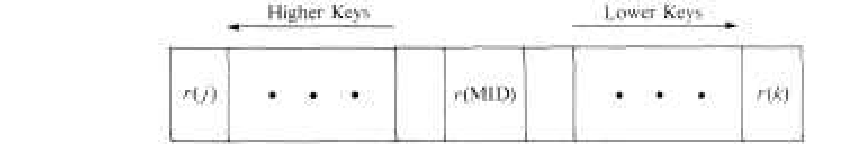
\includegraphics[width=\linewidth]{images/fig-binsearch.png}
\end{image}%
\tcblower
\end{figureptx}%
In the following implementation of the Binary Search in SageMath, we search within a sorted list of integers. Therefore, the items themselves are the keys.%
\begin{sageinput}
def BinarySearch(r,j,k,C):
   found = False
   if j <= k:
      mid = floor((j + k)/2)
      print('probing at position '+str(mid))
      if r[mid] == C:
         location = mid
         found = True
         print('found in position '+str(location))
         return location
      else:
        if r[mid] > C:
           BinarySearch(r,j, mid - 1,C)
        else:
           BinarySearch(r,mid + 1,k,C)
   else:
      print('not found')
      return False      
s=[1,9,13,16,30,31,32,33,36,37,38,45,49,50,52,61,63,64,69,77,79,80,81,83,86,90,93,96]
BinarySearch(s,0,len(s)-1,30)
\end{sageinput}
\begin{sageoutput}
probing at position 13
probing at position 6
probing at position 2
probing at position 4
found in position 4
\end{sageoutput}
\end{subsectionptx}
%
%
\typeout{************************************************}
\typeout{Subsection 8.1.4 Recursively Defined Sequences}
\typeout{************************************************}
%
\begin{subsectionptx}{Recursively Defined Sequences}{}{Recursively Defined Sequences}{}{}{x:subsection:ss-recursive-sequences}
\index{Sequences!Recursively Defined}%
For the next two examples, consider a sequence of numbers to be a list of numbers consisting of a zeroth number, first number, second number, ... . If a sequence is given the name \(S\), the \(k^{th}\) number of \(S\) is usually written \(S_k\)  or \(S(k)\).%
\begin{example}{Geometric Growth Sequence.}{x:example:ex-geometric-growth}%
Define the sequence of numbers \(B\) by%
\begin{equation*}
B_0 = 100\textrm{ and }
\end{equation*}
%
\begin{equation*}
B_k = 1.08 B_{k-1} \textrm{ for } k\geq 1 \text{.}
\end{equation*}
%
\par
These rules stipulate that each number in the list is 1.08 times the previous number, with the starting number equal to 100. For example%
\begin{equation*}
\begin{split}
B_3 &= 1.08 B_2 \\
&=1.08\left(1.08B_1\right)\\
&= 1.08\left(1.08\left(1.08 B_0\right)\right)\\
& = 1.08(1.08(1.08\cdot 100))\\
&= 1.08^3 \cdot 100 = 125.971
\end{split}
\end{equation*}
%
\end{example}
\begin{example}{The Fibonacci Sequence.}{x:example:ex-fibonacci-sequence}%
\index{Fibonacci Sequence}%
The Fibonacci sequence is the sequence \(F\) defined by%
\begin{equation*}
F_0= 1 \textrm{, } F_1= 1\textrm{ and}
\end{equation*}
%
\begin{equation*}
F_k = F_{k-2} + F_{k-1} \textrm{ for }k\geq 2
\end{equation*}
%
\end{example}
\end{subsectionptx}
%
%
\typeout{************************************************}
\typeout{Subsection 8.1.5 Recursion}
\typeout{************************************************}
%
\begin{subsectionptx}{Recursion}{}{Recursion}{}{}{x:subsection:ss-recursion}
All of the previous examples were presented recursively. That is, every ``object'' is described in one of two forms. One form is by a simple definition, which is usually called the basis for the recursion. The second form is by a recursive description in which objects are described in terms of themselves, with the following qualification. What is essential for a proper use of recursion is that the objects can be expressed in terms of simpler objects, where ``simpler'' means closer to the basis of the recursion. To avoid what might be considered a circular definition, the basis must be reached after a finite number of applications of the recursion.%
\par
To determine, for example, the fourth item in the Fibonacci sequence we repeatedly apply the recursive rule for \(F\) until we are left with an expression involving \(F_0\) and \(F_1\):%
\begin{equation*}
\begin{split}
F_4 &= F_2+F_3\\	
&=\left(F_0+F_1\right)+\left(F_1+F_2\right)\\
&=\left(F_0+F_1\right)+\left(F_1+\left(F_0+F_1\right)\right)\\
&=(1+1)+(1+(1+1))\\
&=5
\end{split}
\end{equation*}
%
\end{subsectionptx}
%
%
\typeout{************************************************}
\typeout{Subsection 8.1.6 Iteration}
\typeout{************************************************}
%
\begin{subsectionptx}{Iteration}{}{Iteration}{}{}{x:subsection:ss-iteration}
On the other hand, we could compute a term in the Fibonacci sequence such as \(F_5\) by starting with the basis terms and working forward as follows:%
\begin{tableptx}{\textbf{}}{g:table:idm40467633136}{}%
\centering
{\tabularfont%
\begin{tabular}{l}
\(F_2= F_0+ F_1 =1 + 1 =2\)\tabularnewline[0pt]
\(F_3= F_1+ F_2=1+ 2=3\)\tabularnewline[0pt]
\(F_4= F_2+F_3=2+3=5\)\tabularnewline[0pt]
\(F_5=F_3+F_4= 3+5=8\)
\end{tabular}
}%
\end{tableptx}%
This is called an iterative computation of the Fibonacci sequence. Here we start with the basis and work our way forward to a less simple number, such as 5. Try to compute \(F_5\) using the recursive definition for \(F\) as we did for \(F_4\). It will take much more time than it would have taken to do the computations above. Iterative computations usually tend to be faster than computations that apply recursion. Therefore, one useful skill is being able to convert a recursive formula into a nonrecursive formula, such as one that requires only iteration or a faster method, if possible.%
\par
An iterative formula for \(\binom{n}{k} \) is also much more efficient than an application of the recursive definition. The recursive definition is not without its merits, however. First, the recursive equation is often useful in manipulating algebraic expressions involving binomial coefficients. Second, it gives us an insight into the combinatoric interpretation of \(\binom{n}{k}\). In choosing \(k\) elements from \(\{1, 2,
. . . , n\}\), there are \(\binom{n-1}{k}\) ways of choosing all \(k\) from \(\{1,2, . . . ,n - 1\}\), and there are \(\binom{n-1}{k-1}\) ways of choosing the \(k\) elements if \(n\) is to be selected and the remaining \(k - 1\) elements come from \(\{1, 2, . . . , n - 1\}\). Note how we used the Law of Addition from Chapter 2 in our reasoning.%
\par
\emph{BinarySearch Revisited.} In the binary search algorithm, the place where recursion is used is easy to pick out. When an item is examined and the key is not the one you want, the search is cut down to a sublist of no more than half the number of items that you were searching in before. Obviously, this is a simpler search. The basis is hidden in the algorithm. The two cases that complete the search can be thought of as the basis. Either you find an item that you want, or the sublist that you have been left to search in is empty, when \(j > k\).%
\par
BinarySearch can be translated without much difficulty into any language that allows recursive calls to its subprograms. The advantage to such a program is that its coding would be much shorter than a nonrecursive program that does a binary search. However, in most cases the recursive version will be slower and require more memory at execution time.%
\end{subsectionptx}
%
%
\typeout{************************************************}
\typeout{Subsection 8.1.7 Induction and Recursion}
\typeout{************************************************}
%
\begin{subsectionptx}{Induction and Recursion}{}{Induction and Recursion}{}{}{x:subsection:ss-induction-and-recursion}
\index{Induction and Recursion}%
The definition of the positive integers in terms of Peano's Postulates is a recursive definition. The basis element is the number 1 and the recursion is that if \(n\) is a positive integer, then so is its successor. In this case, \(n\) is the simple object and the recursion is of a forward type. Of course, the validity of an induction proof is based on our acceptance of this definition. Therefore, the appearance of induction proofs when recursion is used is no coincidence.%
\begin{example}{Proof of a formula for \(B\).}{x:example:ex-geometric-squence-proof}%
A formula for the sequence \(B\) in \hyperref[x:example:ex-geometric-growth]{Example~{\xreffont\ref{x:example:ex-geometric-growth}}} is \(B = 100(1.08)^k\) for \(k\geq 0\). A proof by induction follow.%
\par
If \(k= 0\), then \(B = 100(1.08)^0 = 100\), as defined. Now assume that for some \(k\geq 1\), the formula for \(B_k\) is true.%
\begin{equation*}
\begin{split}
B_{k+1} &= 1.08B_k \textrm{  by the recursive definition}\\
&=1.08\left(100 (1.08)^k\right) \textrm{  by the induction hypothesis}\\ 
&= 100 (1.08)^{k+1}
\end{split}
\end{equation*}
hence the formula is true for \(k+1\)%
\par
The formula that we have just proven for \(B\) is called a closed form expression. It involves no recursion or summation signs.%
\end{example}
\begin{definition}{Closed Form Expression.}{x:definition:def-closed-form-expression}%
\index{Closed Form Expression.}%
Let \(E = E\left(x_1, x_2, \ldots ,x_n\right)\) be an algebraic expression involving variables \(x_1, x_2, \ldots ,x_n\) which are allowed to take on values from some predetermined set. \(E\) is a \terminology{closed form expression} if there exists a number \(T\) such that the evaluation of \(E\) with any allowed values of the variables will take no more than \(T\) operations (alternatively, \(T\) time units).%
\end{definition}
\begin{example}{Reducing a summation to closed form.}{x:example:ex-summation-simplifed}%
The sum \(E(n)=\sum_{k=1}^n k\) is not a closed form expression because the number of additions needed to evaluate \(E(n)\) grows indefinitely with \(n\). A closed form expression that computes the value of \(E(n)\) is \(\frac{n(n+1)}{2}\), which only requires \(T=3\) operations.%
\end{example}
\end{subsectionptx}
%
%
\typeout{************************************************}
\typeout{Exercises 8.1.8 Exercises}
\typeout{************************************************}
%
\begin{exercises-subsection}{Exercises}{}{Exercises}{}{}{g:exercises:idm40467604720}
\begin{divisionexercise}{1}{}{}{g:exercise:idm40467602176}%
By the recursive definition of binomial coefficients, \(\binom{7}{2}=\binom{6}{2} +\binom{6}{1}\). Continue expanding \(\binom{7}{2}\) to express it in terms of quantities defined by the basis. Check your result by applying the factorial definition of \(\binom{n}{k}\).%
\end{divisionexercise}%
\begin{divisionexercise}{2}{}{}{g:exercise:idm40467601536}%
Define the sequence \(L\) by \(L_0 = 5\) and for \(k\geq 1\), \(L _k = 2L_{k-1}-7\).  Determine \(L_4\) and prove by induction that \(L_k=7-2^{k+1}\).%
\end{divisionexercise}%
\begin{divisionexercise}{3}{}{}{g:exercise:idm40467597456}%
Let \(p(x) = x^5+ 3x^4 - 15x^3 + x - 10\).%
\par
%
\begin{enumerate}[label=(\alph*)]
\item{}Write \(p(x)\) in telescoping form.%
\item{}Use a calculator to compute \(p(3)\) using the original form of \(p(x)\).%
\item{}Use a calculator to compute \(p(3)\) using the telescoping form of \(p(x)\).%
\item{}Compare your speed in parts b and c.%
\end{enumerate}
%
\end{divisionexercise}%
\begin{divisionexercise}{4}{}{}{g:exercise:idm40467586368}%
Suppose that a list of nine items, \((r(l), r(2), . . . , r(9))\), is sorted by key in decending order so that \(r(3).\texttt{key} = 12\) and \(r(4).\texttt{key} = 10\). List the executions of the BinarySearch algorithms that would be needed to complete BinarySearch(1,9) when:%
\begin{multicols}{2}
\begin{enumerate}[label=(\alph*)]
\item{}The search key is C = 12%
\item{}The search key is C = 11%
\end{enumerate}
\end{multicols}
%
\par
Assume that distinct items have distinct keys.%
\end{divisionexercise}%
\begin{divisionexercise}{5}{}{}{g:exercise:idm40467582640}%
What is wrong with the following definition of \(f:\mathbb{R}\to \mathbb{R}\)? \(f(0) = 1\) and \(f(x) = f(x/2)/2\) if \(x\neq 0\).%
\end{divisionexercise}%
\begin{divisionexercise}{6}{}{}{g:exercise:idm40467578816}%
Prove the two definitions of binomials coefficients, \hyperref[x:definition:binomial-coefficient]{Definition~{\xreffont\ref{x:definition:binomial-coefficient}}} and \hyperref[x:definition:def-binomial-coefficient-recursive]{Definition~{\xreffont\ref{x:definition:def-binomial-coefficient-recursive}}}, are equivalent.%
\end{divisionexercise}%
\begin{divisionexercise}{7}{}{}{x:exercise:exercise-binomial-sum}%
Prove by induction that if \(n \geq 0\), \(\sum_{k=0}^n \binom{n}{k} = 2^n\)%
\end{divisionexercise}%
\end{exercises-subsection}
\end{sectionptx}
%
%
\typeout{************************************************}
\typeout{Section 8.2 Sequences}
\typeout{************************************************}
%
\begin{sectionptx}{Sequences}{}{Sequences}{}{}{x:section:s-Sequences}
\index{Sequences}%
%
%
\typeout{************************************************}
\typeout{Subsection 8.2.1 Sequences and Ways They Are Defined}
\typeout{************************************************}
%
\begin{subsectionptx}{Sequences and Ways They Are Defined}{}{Sequences and Ways They Are Defined}{}{}{g:subsection:idm40467573984}
\begin{definition}{Sequence.}{x:definition:def-sequence}%
\index{Sequence}%
A sequence is a function from the natural numbers into some predetermined set. The image of any natural number \(k\) can be written  as \(S(k)\) or \(S_k\) and is called the \(k^{th}\)  \emph{term}  of \(S\). The variable \(k\) is called the  \emph{index}  or  \emph{argument}  of the sequence.%
\end{definition}
For example, a sequence of integers would be a function \(S:\mathbb{N}\to \mathbb{Z}\).%
\begin{example}{Three sequences defined in different ways.}{x:example:ex-three-sequences}%
%
\begin{enumerate}[label=(\alph*)]
\item{}The sequence \(A\) defined by \(A(k) = k^2 - k\),  \(k \geq  0\), is a sequence of integers.%
\item{}The sequence \(B\) defined recursively by \(B(0) = 2\) and \(B(k) = B(k - 1) + 3\) for \(k \geq  1\) is a sequence of integers. The terms of \(B\) can be computed either by applying the recursion formula or by iteration. For example,%
\begin{equation*}
\begin{split}
B(3)  &= B(2) + 3\\
& =(B(1)+3)+3\\
& = ((B(0)+3)+3)+3\\
&=((2+3)+3)+3=11
\end{split}
\end{equation*}
or%
\begin{equation*}
\begin{array}{c}
B(1) = B(0) + 3 = 2 + 3 = 5\\
B(2) = B(1) + 3 = 5 + 3 = 8\\
B(3) = B(2) + 3 = 8 + 3 = 11
\end{array}
\end{equation*}
%
\item{}Let \(C_r\) be the number of strings of 0's and 1's of length \(r\) having no consecutive zeros. These terms define a sequence \(C\) of integers.%
\end{enumerate}
%
\end{example}
Remarks:%
\par
%
\begin{enumerate}[label=(\arabic*)]
\item{}A sequence is often called a  \emph{discrete function}.%
\item{}Although it is important to keep in mind that a sequence is a function, another useful way of visualizing a sequence is as a list. For example, the sequence \(A\) in the previous example could be written as \((0, 0, 2, 6, 12, 20, \dots )\). Finite sequences can appear much the same way when they are the input to or output from a computer. The index of a sequence can be thought of as a time variable. Imagine the terms of a sequence flashing on a screen every second. Then \(s_k\) would be what you see in the \(k^{th}\) second. It is convenient to use terminology like this in describing sequences. For example, the terms that precede the \(k^{th}\) term of \(A\) would be \(A (0), A(1), . . . , A(k -1)\).  They might be called the earlier terms.%
\end{enumerate}
%
\end{subsectionptx}
%
%
\typeout{************************************************}
\typeout{Subsection 8.2.2 A Fundamental Problem}
\typeout{************************************************}
%
\begin{subsectionptx}{A Fundamental Problem}{}{A Fundamental Problem}{}{}{g:subsection:idm40467556848}
Given the definition of any sequence, a fundamental problem that we will concern ourselves with is to devise a method for determining any specific term in a minimum amount of time. Generally, time can be equated with the number of operations needed. In counting operations, the application of a recursive formula would be considered an operation.%
\par
%
\begin{enumerate}[label=(\alph*)]
\item{}The terms of \(A\) in \hyperref[x:example:ex-three-sequences]{Example~{\xreffont\ref{x:example:ex-three-sequences}}} are very easy to compute because of the closed form expression. No matter what term you decide to compute, only three operations need to be performed.%
\item{}How to compute the terms of \(B\) is not so clear. Suppose that you wanted to know \(B(100)\). One approach would be to apply the definition recursively:%
\begin{equation*}
B(100) = B(99) + 3 = (B(98) + 3) + 3 =\cdots
\end{equation*}
The recursion equation for \(B\) would be applied 100 times and 100 additions would then follow. To compute \(B(k)\) by this method, \(2k\) operations are needed. An iterative computation of \(B(k)\) is an improvement: \(B(1) =B(0) +3 = 2 + 3 = 5\\
\\
B(2) =B(1)+3= 5 + 3 = 8\\
\\
\text{etc}.\) Only \(k\) additions are needed. This still isn't a good situation. As \(k\) gets large, we take more and more time to compute \(B(k)\).  The formula \(B(k)=B(k-1)+3\) is called a recurrence relation on \(B\). The process of finding a closed form expression for \(B(k)\), one that requires no more than some fixed number of operations, is called solving the recurrence relation.%
\item{}The determination of \(C_k\) is a standard kind of problem in combinatorics. One solution is by way of a recurrence relation. In fact, many problems in combinatorics are most easily solved by first searching for a recurrence relation and then solving it. The following observation will suggest the recurrence relation that we need to determine \(C_k\). If \(k \geq  2\), then every string of 0's and 1's with length \(k\) and no two consecutive 0's is either \(1s_{k-1}\) or \(01s_{k-2}\), where \(s_{k-1}\) and \(s_{k-2}\) are strings with no two consecutive 0's of length \(k - 1\) and \(k - 2\) respectively. From this observation we can see that \(C_k= C_{k-2}+C_{k-1}\) for \(k\geq 2\). The terms \(C_0=
1\) and \(C_1 = 2\) are easy to determine by enumeration. Now, by iteration, any \(C_k\) can be easily determined. For example, \(C_5 = 21\) can be computed with five additions. A closed form expression for \(C_k\) would be an improvement. Note that the recurrence relation for \(C_k\) is identical to the one for \hyperref[x:example:ex-fibonacci-sequence]{The Fibonacci Sequence}. Only the basis is different.%
\end{enumerate}
%
\end{subsectionptx}
%
%
\typeout{************************************************}
\typeout{Exercises 8.2.3 Exercises}
\typeout{************************************************}
%
\begin{exercises-subsection}{Exercises}{}{Exercises}{}{}{x:exercises:exercises-8-2}
\begin{divisionexercise}{1}{}{}{g:exercise:idm40467533184}%
Prove by induction that \(B(k) = 3k + 2,\) \(k\geq 0\), is a closed form expression for the sequence \(B\) in \hyperref[x:example:ex-three-sequences]{Example~{\xreffont\ref{x:example:ex-three-sequences}}}%
\end{divisionexercise}%
\begin{divisionexercise}{2}{}{}{g:exercise:idm40467527840}%
%
\begin{enumerate}[label=(\alph*)]
\item{}Consider sequence \(Q\) defined by \(Q(k) = 2k + 9\), \(k \geq  1\). Complete the table below and determine a recurrence relation that describes \(Q\). \(\begin{array}{c|c|c}
k & Q(k)  & Q(k)-Q(k-1) \\
\hline
2 &   &   \\
3 &   &   \\
4 & \text{  } &   \\
5 &   &   \\
6 &   &   \\
7 &   &   \\
\end{array}\)%
\item{}Let \(A(k) = k^2 - k\), \(k \geq  0\). Complete the table below and determine a recurrence relation for \(A\).%
\begin{equation*}
\begin{array}{c|c|c|c}
k & A(k) & A(k)-A(k-1) & A(k)-2A(k-1)+A(k-2) \\
\hline
2 &   &   &   \\
3 &   &   &   \\
4 &   &   &   \\
5 &   &   &   \\
\end{array}
\end{equation*}
%
\end{enumerate}
%
\end{divisionexercise}%
\begin{divisionexercise}{3}{}{}{g:exercise:idm40467521408}%
Given \(k\) lines (\(k\geq 0\)) on a plane such that no two lines are parallel and no three lines meet at the same point, let \(P(k)\) be the number of regions into which the lines divide the plane (including the infinite ones (see \hyperref[x:figure:exercise-8-2-3]{Figure~{\xreffont\ref{x:figure:exercise-8-2-3}}}). Describe how the recurrence relation \(P(k) = P(k - 1) + k\) can be derived. Given that \(P(0) = 1\), determine \(P(5)\).%
\begin{figureptx}{A general configuration of three lines}{x:figure:exercise-8-2-3}{}%
\begin{image}{0.2}{0.6}{0.2}%
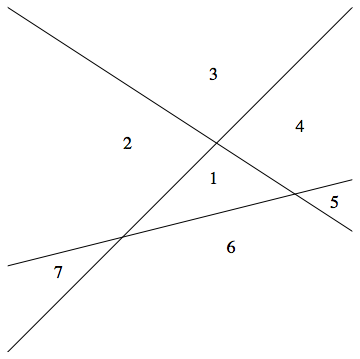
\includegraphics[width=\linewidth]{images/exercise-8-2-3.png}
\end{image}%
\tcblower
\end{figureptx}%
\end{divisionexercise}%
\begin{divisionexercise}{4}{}{}{g:exercise:idm40467515520}%
A sample of a radioactive substance is expected to decay by 0.15 percent each hour. If \(w_t,\) \(t \geq  0\), is the weight of the sample \(t\) hours into an experiment, write a recurrence relation for \(w\).%
\end{divisionexercise}%
\begin{divisionexercise}{5}{}{}{g:exercise:idm40467509296}%
Let \(M(n)\) be the number of multiplications needed to evaluate an \(n^{th}\) degree polynomial. Use the recursive definition of a polynomial expression to define \(M\) recursively.%
\end{divisionexercise}%
\end{exercises-subsection}
\end{sectionptx}
%
%
\typeout{************************************************}
\typeout{Section 8.3 Recurrence Relations}
\typeout{************************************************}
%
\begin{sectionptx}{Recurrence Relations}{}{Recurrence Relations}{}{}{x:section:s-recurrence-relations}
\begin{introduction}{}%
In this section we will begin our study of recurrence relations and their solutions. Our primary focus will be on the class of finite order linear recurrence relations with constant coefficients (shortened to finite order linear relations). First, we will examine closed form expressions from which these relations arise. Second, we will present an algorithm for solving them. In later sections we will consider some other common relations (8.4) and introduce two additional tools for studying recurrence relations: generating functions (8.5) and matrix methods (Chapter 12).%
\end{introduction}%
%
%
\typeout{************************************************}
\typeout{Subsection 8.3.1 Definition and Terminology}
\typeout{************************************************}
%
\begin{subsectionptx}{Definition and Terminology}{}{Definition and Terminology}{}{}{x:subsection:defs-rr}
\begin{definition}{Recurrence Relation.}{x:definition:def-recurrence-relation}%
\index{Recurrence Relation}%
Let \(S\) be a sequence of numbers.  A recurrence relation on \(S\) is a formula that relates all but a finite number of terms of \(S\) to previous terms of \(S\). That is, there is a \(k_0\) in the domain of \(S\) such that if \(k \geq  k_0\), then \(S(k)\) is expressed in terms of some (and possibly all) of the terms that precede \(S(k)\). If the domain of \(S\) is \(\{0,1,2,\dots \}\), the terms \(S
(0), S(1), . . . , S\left(k_0-1\right)\) are not defined by the recurrence formula. Their values are the initial conditions (or boundary conditions, or basis) that complete the definition of \(S\).%
\end{definition}
\begin{example}{Some Examples of Recurrence Relations.}{x:example:ex-some-recurrence-relations}%
%
\begin{enumerate}[label=(\alph*)]
\item{}The Fibonacci sequence is defined by the recurrence relation \(F_k= F_{k-2}+ F_{k-1}\), \(k\geq 2,\) with the initial conditions \(F_0=1\) and \(F_1=1\). The recurrence relation is called a second-order relation because \(F_k\) depends on the two previous terms of \(F\). Recall that the sequence \(C\) in Section 8.2, \hyperref[x:example:ex-three-sequences]{Example~{\xreffont\ref{x:example:ex-three-sequences}}}, can be defined with the same recurrence relation, but with different initial conditions.%
\item{}The relation \(T(k) = 2T(k - 1)^2 - k T(k - 3)\) is a third-order recurrence relation. If values of \(T(0)\), \(T(1)\), and \(T(2)\) are specified, then \(T\) is completely defined.%
\item{}The recurrence relation \(S(n) = S(\lfloor n/2\rfloor ) + 5\), \(n > 0\), with \(S(0)=0\) has infinite order. To determine \(S(n)\) when \(n\) is even, you must go back \(n/2\) terms. Since \(n/2\) grows unbounded with \(n\), no finite order can be given to \(S\).%
\end{enumerate}
%
\end{example}
\end{subsectionptx}
%
%
\typeout{************************************************}
\typeout{Subsection 8.3.2 Solving Recurrence Relations}
\typeout{************************************************}
%
\begin{subsectionptx}{Solving Recurrence Relations}{}{Solving Recurrence Relations}{}{}{x:subsection:ss-solving-recurrence-relations}
\index{Recurrence Relations!Solving}%
Sequences are often most easily defined with a recurrence relation; however, the calculation of terms by directly applying a recurrence relation can be time-consuming. The process of determining a closed form expression for the terms of a sequence from its recurrence relation is called solving the relation. There is no single technique or algorithm that can be used to solve all recurrence relations. In fact, some recurrence relations cannot be solved. The relation that defines \(T\) above is one such example. Most of the recurrence relations that you are likely to encounter in the future are classified as finite order linear recurrence relations with constant coefficients. This class is the one that we will spend most of our time with in this chapter.%
\begin{definition}{\(n^{th}\) Order Linear Recurrence Relation.}{x:definition:def-n-th-order-rr}%
\index{Order of a Recurrence Relation}%
Let \(S\) be a sequence of numbers with domain \(k\geq 0\). An \(n^{\textrm{th}}\) order linear recurrence relation on \(S\) with constant coefficients is a recurrence relation that can be written in the form%
\begin{equation*}
S(k) + C_1 S(k - 1) + . . . + C_n S(k - n) = f(k)\textrm{  for  }k \geq  n
\end{equation*}
where \(C_1, C_2, \ldots , C_n\) are constants and \(f\) is a numeric function that is defined for \(k \geq n\).%
\end{definition}
Note: We will shorten the name of this class of relations to \(n^{\textrm{th}}\) order linear relations. Therefore, in further discussions, \(S(k)
+ 2k S(k - 1) = 0\) would not be considered a first-order linear relation.%
\begin{example}{Some Finite Order Linear  Relations.}{x:example:ex-some-finite-order-rr}%
%
\begin{enumerate}[label=(\alph*)]
\item{}The Fibonacci sequence is defined by the second-order linear relation because \(F_k- F_{k-1}- F_{k-2}=0\)%
\item{}The relation \(P(j) + 2P(j - 3) = j^2\) is a third-order linear relation. In this case, \(C_1= C_2= 0\).%
\item{}The relation \(A(k)= 2(A(k - 1) + k)\) can be written as \(A(k) - 2A(k - 1) = 2k\). Therefore, it is a first-order linear relation.%
\end{enumerate}
%
\end{example}
\end{subsectionptx}
%
%
\typeout{************************************************}
\typeout{Subsection 8.3.3 Recurrence relations obtained from ``solutions''}
\typeout{************************************************}
%
\begin{subsectionptx}{Recurrence relations obtained from ``solutions''}{}{Recurrence relations obtained from ``solutions''}{}{}{x:subsection:sss-recurrence-relations-obtained-from-solutions}
\index{Recurrence relations obtained from ``solutions''}%
Before giving an algorithm for solving finite order linear relations, we will examine recurrence relations that arise from certain closed form expressions. The closed form expressions are selected so that we will obtain finite order linear relations from them. This approach may seem a bit contrived, but if you were to write down a few simple algebraic expressions, chances are that most of them would be similar to the ones we are about to examine.%
\par
For our first example, consider \(D\), defined by \(D(k) =5\cdot 2^k\), \(k \geq  0\). If \(k \geq  1\), \(\quad\)\(D(k) =5\cdot 2^k = 2\cdot 5\cdot 2^{k-1} = 2 D(k - 1)\). Therefore, \(D\) satisfies the first order linear relation \(D(k) - 2 D(k - 1) = 0\) and the initial condition \(D(0) = 5\) serves as an initial condition for \(D\).%
\par
As a second example, consider \(C(k) =3^{k-1}+2^{k+1}+k\) , \(k \geq  0\). Quite a bit more algebraic manipulation is required to get our result:%
\begin{tableptx}{\textbf{}}{g:table:idm40467460976}{}%
\centering
{\tabularfont%
\begin{tabular}{ll}\hrulethick
\(C(k) =3^{k-1}+2^{k+1}+k\)&\(\textrm{Original equation}\)\tabularnewline[0pt]
\(3C(k-1) =3^{k-1}+3\cdot 2^k+3(k-1)\)&\(\textrm{Substitute } k-1 \textrm{ for } k \)\tabularnewline[0pt]
&\(\textrm{ and multiply by } 3\)\tabularnewline[0pt]
\(\)&\(\textrm{Subtract the second equation}\)\tabularnewline[0pt]
&\(\textrm{from the first.}\)\tabularnewline[0pt]
\(C(k)-3C(k-1)=-2^k-2k+3\)&\(3^{k-1} \textrm{ term  is eliminated.} \)\tabularnewline[0pt]
&\(\textrm{ This is  a  first order relation}\).\tabularnewline[0pt]
\(2C(k-1)-6C(k-2)=-2^k-2(2(k-1))+6\)&\(\textrm{Substitute } k-1 \textrm{ for } k \textrm{ in the}\)\tabularnewline[0pt]
&\(\textrm{third equation, multiply by } 2\).\tabularnewline[0pt]
\(\)&\(\textrm{Subtract the 4th equation from the 3rd.}\)\tabularnewline[0pt]
\(C(k)-5C(k-1)+6C(k-2)=2k-7\)&\(2^{k+1}\textrm{term is eliminated.}\)\tabularnewline[0pt]
&\(\textrm{This is 2nd order relation.}\)
\end{tabular}
}%
\end{tableptx}%
The recurrence relation that we have just obtained, defined for \(k \geq  2\), together with the initial conditions \(C(0) = 7/3\) and \(C(1) = 6\), define \(C\).%
\par
\hyperref[x:table:table-reverse-solutions-rr]{Table~{\xreffont\ref{x:table:table-reverse-solutions-rr}}} summarizes our results together with a few other examples that we will let the reader derive. Based on these results, we might conjecture that any closed form expression for a sequence that combines exponential expressions and polynomial expressions will be solutions of finite order linear relations. Not only is this true, but the converse is true: a finite order linear relation defines a closed form expression that is similar to the ones that were just examined. The only additional information that is needed is a set of initial conditions.%
\begin{tableptx}{\textbf{Recurrence relations obtained from given sequences}}{x:table:table-reverse-solutions-rr}{}%
\centering
{\tabularfont%
\begin{tabular}{cc}\hrulethick
Closed Form Expression&Recurrence Relation\tabularnewline[0pt]
\(D(k)=5\cdot 2^k\)&\(D(k)-2D(k-1)=0\)\tabularnewline[0pt]
\(C(k)=3^{k-1}+2^{k+1}+k\)&\(C(k)-2C(k-1)-6C(k-2)=2k-7\)\tabularnewline[0pt]
\(Q(k)=2k + 9\)&\(Q(k)-Q(k-1)=2\)\tabularnewline[0pt]
\(A(k)=k^2-k\)&\(A(k)-2A(k-1)+A(k-2)=2\)\tabularnewline[0pt]
\(B(k)=2 k^2+1\)&\(B(k)-2B(k-1)+B(k-2)=4\)\tabularnewline[0pt]
\(G(k)=2\cdot 4^k-5(-3)^k\)&\(G(k)-G(k-1)+12G(k-2)=0\)\tabularnewline[0pt]
\(J(k)=(3+k) 2^k\)&\(J(k)-4J(k-1)+4J(k-2)=0\)
\end{tabular}
}%
\end{tableptx}%
\begin{definition}{Homogeneous Recurrence Relation.}{x:definition:def-homogeneous-recurrence-relation}%
\index{Homogeneous Recurrence Relation.}%
An \(n^{th}\) order linear relation is homogeneous if \(f(k)
= 0\) for all \(k\). For each recurrence relation \(S(k) + C_1S(k - 1) +\ldots + C_n S(k - n) = f(k)\), the associated homogeneous relation is \(S(k)
+ C_1S(k - 1) +\ldots + C_n S(k - n) =0\)%
\end{definition}
\begin{example}{First Order Homogeneous Recurrence Relations.}{x:example:ex-first-order-homogeneous-rr}%
\(D(k) - 2D(k - 1) = 0\) is a first-order homogeneous relation. Since it can also be written as \(D(k) = 2D(k - 1)\), it should be no surprise that it arose from an expression that involves powers of 2. More generally, you would expect that the solution of \(L(k) - a L(k - 1)\) would involve \(a^k\). Actually, the solution is \(L(k) = L(0)a^k\), where the value of \(L(0)\) is given by the initial condition.%
\end{example}
\begin{example}{A Second Order Example.}{x:example:ex-second-order-rr}%
Consider the second-order homogeneous relation \(S(k) - 7S(k - 1) + 12 S(k- 2) = 0\) together with the initial conditions \(S(0) = 4\) and \(S(1) = 4\). From our discussion above, we can predict that the solution to this relation involves terms of the form \(b a^k\), where \(b\) and \(a\) are nonzero constants that must be determined. If the solution were to equal this quantity exactly, then%
\begin{equation*}
\quad \quad \quad  \begin{array}{ccc}
S(k)=b a^k &   &   \\
S(k-1)=b a^{k-1} & \textrm{   } & \textrm{  } \\
S(k-2)=b a^{k-2} &   &   \\
\end{array}
\end{equation*}
Substitute these expressions into the recurrence relation to get%
\begin{equation*}
b a^k-7 b a^{k-1}+12 b a^{k-2}=0
\end{equation*}
Each term on the left-hand side of this equation has a factor of \(b a^{k-2}\), which is nonzero. Dividing through by this common factor yields%
\begin{gather}
a^2 - 7a + 12 = (a - 3) (a - 4) = 0\label{x:mrow:eq-characteristic-example}
\end{gather}
%
\par
Therefore, the only possible values of \(a\) are 3 and 4. Equation \hyperref[x:mrow:eq-characteristic-example]{({\xreffont\ref{x:mrow:eq-characteristic-example}})} is called the characteristic equation of the recurrence relation. The fact is that our original recurrence relation is true for any sequence of the form \(S(k) = b_1 3^k + b_24^k\), where \(b_1\) and \(b_2\) are real numbers. This set of sequences is called the general solution of the recurrence relation. If we didn't have initial conditions for \(S\), we would stop here. The initial conditions make it possible for us to find definite values for \(b_1\) and \(b_2\).%
\begin{equation*}
\left\{
\begin{array}{c}
S(0)=4 \\
S(1)=4 \\
\end{array}
\right\}\textrm{  }\Rightarrow \left\{
\begin{array}{c}
b_13^0+b_24^0=4 \\
b_13^1+b_24^1=4 \\
\end{array}
\right\}\textrm{  }\Rightarrow \left\{
\begin{array}{c}
b_1+b_2=4 \\
3b_1+4b_2=4 \\
\end{array}
\right\}\textrm{  }
\end{equation*}
%
\par
The solution of this set of simultaneous equations is \(b_1 = 12\) and \(b_2 = -8\) and so the solution is \(S(k) = 12 \cdot 3^k - 8 \cdot 4^k\).%
\end{example}
\begin{definition}{Characteristic Equation.}{x:definition:def-characteristic-equation}%
\index{Characteristic Equation}%
\index{Characteristic Roots}%
The characteristic equation of the homogeneous \(n^{\textrm{th}}\) order linear relation \(S(k) + C_1 S(k- 1) +\ldots + C_n S(k - n) =0\) is the \(n\)th degree polynomial equation%
\begin{equation*}
a^n+\sum_{j=1}^n C_j a^{n-j}=a^n+ C_1a^{n-1}+\cdots +C_{n-1}a+C_n=0
\end{equation*}
The left-hand side of this equation is called the characteristic polynomial.  The roots of the characteristic polynomial are called the characteristic roots of the equation.%
\end{definition}
\begin{example}{Some characteristic equations.}{x:example:ex-some-char-equations}%
%
\begin{enumerate}[label=(\alph*)]
\item{}The characteristic equation of \(F(k) - F(k - 1) - F(k - 2) = 0\) is \(a^2-a-1=0\).%
\item{}The characteristic equation of \(Q(k) + 2Q(k - 1) - 3Q(k - 2) - 6 Q(k- 4) = 0\) is \(a^4+ 2a^3 - 3a^2 - 6 = 0.\) Note that the absence of a \(Q(k - 3)\) term means that there is not an \(x^{4-3}=x\) term appearing in the characteristic equation.%
\end{enumerate}
%
\end{example}
\begin{algorithm}{Algorithm for Solving Homogeneous Finite Order Linear Relations.}{}{x:algorithm:algorithm-linear-homogeneous-recurrence-relations}%
%
\begin{enumerate}[label=(\alph*)]
\item{}Write out the characteristic equation of the relation \(S(k) + C_1S(k - 1) +\ldots + C_n S(k - n) =0\), which is \(a^n+ C_1a^{n-1}+\cdots
+C_{n-1}a+C_n=0\).%
\item{}Find all roots of the characteristic equation, the characteristic roots.%
\item{}If there are \(n\) distinct characteristic roots, \(a_1, a_2, \dots a_n\), then the general solution of the recurrence relation is \(S(k) = b_1a_1{}^k+ b_2a_2{}^k+\cdots +b_na_n{}^k\). If there are fewer than \(n\) characteristic roots, then at least one root is a multiple root. If \(a_j\) is a double root, then the \(b_ja_j{}^k\) term is replaced with \(\left(b_{j 0}+b_{j 1}k\right)a_j^{k}\textrm{.}\) In general, if \(a_j\) is a root of multiplicity \(p\), then the \(b_ja_j{}^k\) term is replaced with \(\left(b_{j 0}+b_{j 1}k+\cdots +b_{j(p-1)}k^{p-1}\right)a_j^{k}\).%
\item{}If \(n\) initial conditions are given, we get \(n\) linear equations in \(n\) unknowns (the \({b_j}'s\) from Step 3) by substitution. If possible, solve these equations to determine a final form for \(S(k)\).%
\end{enumerate}
%
\end{algorithm}
Although this algorithm is valid for all values of \(n\), there are limits to the size of \(n\) for which the algorithm is feasible. Using just a pencil and paper, we can always solve second-order equations. The quadratic formula for the roots of \(a x^2 + b x + c = 0\) is%
\begin{equation*}
x=\frac{-b\pm \sqrt{b^2-4 a c}}{2 a}
\end{equation*}
The solutions of \(a^2+ C_1a + C_2 = 0\) are then%
\begin{equation*}
\frac{1}{2}\left(-C_1+\sqrt{C_1{}^2-4 C_2}\right)\textrm{ and }\frac{1}{2}\left(-C_1-\sqrt{C_1{}^2-4 C_2}\right)
\end{equation*}
%
\par
Although cubic and quartic formulas exist, they are too lengthy to introduce here. For this reason, the only higher-order relations (\(n\geq 3\)) that you could be expected to solve by hand are ones for which there is an easy factorization of the characteristic polynomial.%
\begin{example}{A solution using the algorithm.}{x:example:ex-hrr-solution-example-1}%
Suppose that \(T\) is defined by \(T(k) =7T(k-1)-10T(k-2)\), with \(T(0) = 4\) and \(T(1) = 17\). We can solve this recurrence relation with \hyperref[x:algorithm:algorithm-linear-homogeneous-recurrence-relations]{Algorithm~{\xreffont\ref{x:algorithm:algorithm-linear-homogeneous-recurrence-relations}}}:%
\par
%
\begin{enumerate}[label=(\alph*)]
\item{}Note that we have written the recurrence relation in ``nonstandard'' form. To avoid errors in this easy step, you might consider a rearrangement of the equation to, in this case, \(T(k) -7T(k-1)+10T(k-2)=0\). Therefore, the characteristic equation is \(a^2 -7a + 10 = 0\).%
\item{}The characteristic roots are \(\frac{1}{2}\left(7+\sqrt{49-40}\right)=5\) and \(\frac{1}{2}\left(7-\sqrt{49-40}\right)=2\). These roots can be just as easily obtained by factoring the characteristic polynomial into \((a - 5)(a - 2)\).%
\item{}The general solution of the recurrence relation is \(T(k) =b_12^k+ b_25^k\).%
\item{}\(\quad\) \(\left\{
\begin{array}{c}
T(0)=4 \\
T(1)=17 \\
\end{array}
\right\}\textrm{  }\Rightarrow \left\{
\begin{array}{c}
b_12^0+b_25^0=4 \\
b_12^1+b_25^1=17 \\
\end{array}
\right\}\textrm{  }\Rightarrow \left\{
\begin{array}{c}
b_1+b_2=4 \\
2b_1+5b_2=17 \\
\end{array}
\right\}\textrm{  }\) The simultaneous equations have the solution \(b_1=1\) and \(b_2=3\). Therefore, \(T(k)=2^{k }+3\cdot 5^k\).%
\end{enumerate}
%
\end{example}
Here is one rule that might come in handy: If the coefficients of the characteristic polynomial are all integers, with the constant term equal to \(m\), then the only possible rational characteristic roots are divisors of \(m\) (both positive and negative).%
\par
With the aid of a computer (or possibly only a calculator), we can increase \(n\). Approximations of the characteristic roots can be obtained by any of several well-known methods, some of which are part of standard software packages. There is no general rule that specifies the values of \(n\) for which numerical approximations will be feasible. The accuracy that you get will depend on the relation that you try to solve. (See Exercise 17 of this section.)%
\begin{example}{Solution of a Third Order Recurrence Relation.}{x:example:ex-hrr-solution-example-2}%
Solve \(S(k) - 7S(k - 2) + 6S(k - 3) = 0\), where \(S(0) =8\), \(S(1) = 6\), and \(S(2) = 22\).%
\par
%
\begin{enumerate}[label=(\alph*)]
\item{}The characteristic equation is \(a^3 - 7a + 6 = 0\).%
\item{}The only rational roots that we can attempt are \(\pm  1, \pm 2, \pm 3, \textrm{and} \pm 6\). By checking these, we obtain the three roots 1, 2, and \(-3\).%
\item{}The general solution is \(S(k) =b_11^k+b_22^k+b_3(-3){}^k\). The first term can simply be written \(b_1\) .%
\item{}\(\left\{
\begin{array}{c}
S(0)=8 \\
S(1)=6 \\
S(2)=22 \\
\end{array}
\right\}\textrm{   }\Rightarrow \left\{
\begin{array}{c}
b_1+b_2+b_3=8 \\
b_1+2b_2-3b_3=6 \\
b_1+4b_2+9b_3=22 \\
\end{array}
\right\}\textrm{  }\) You can solve this system by elimination to obtain \(b_1=5\), \(b_2=2\), and \(b_3=1\). Therefore, \(\quad\)\(S(k) = 5 + 2\cdot 2^k + (-3)^k = 5 + 2^{k+1} + (-3)^k\)%
\end{enumerate}
%
\end{example}
\begin{example}{Solution with a Double Characteristic Root.}{x:example:ex-hrr-solution-example-3}%
Solve \(D(k) - 8D(k - 1) + 16D(k - 2) = 0\), where \(D(2) = 16\) and \(D(3) = 80\).%
\par
%
\begin{enumerate}[label=(\alph*)]
\item{}Characteristic equation: \(a^2- 8a + 16 = 0\).%
\item{}\(a^2- 8a + 16 = (a - 4)^2\). Therefore, there is a double characteristic root, 4.%
\item{}General solution: \(D(k) = \left(b_{10}+b_{11}k\right)4^k\).%
\item{}\(\left\{
\begin{array}{c}
D(2)=16 \\
D(3)=80 \\
\end{array}
\right\}\textrm{  }\Rightarrow \left\{
\begin{array}{c}
\left(b_{10}+b_{11}2\right)4^2=16 \\
\left(b_{10}+b_{11}3\right)4^3=80 \\
\end{array}
\right\}\textrm{  } \\ \Rightarrow \left\{
\begin{array}{c}
16b_{10}+32b_{11}=16 \\
64b_{10}+192b_{11}=80 \\
\end{array}
\right\} \Rightarrow  \left\{
\begin{array}{c}
b_{10}=\frac{1}{2} \\
b_{11}=\frac{1}{4} \\
\end{array}
\right\}\)%
\par
Therefore \(D (k) = (1/2 + (1/4) k) 4^k= (2 + k)4^{k-1}\).%
\end{enumerate}
%
\end{example}
\end{subsectionptx}
%
%
\typeout{************************************************}
\typeout{Subsection 8.3.4 Solution of Nonhomogeneous Finite Order Linear Relations}
\typeout{************************************************}
%
\begin{subsectionptx}{Solution of Nonhomogeneous Finite Order Linear Relations}{}{Solution of Nonhomogeneous Finite Order Linear Relations}{}{}{x:subsection:ss-solution-of-nonhomogeneous-relations}
\index{Nonhomogeneous of Finite Order Linear Relations!Solution}%
Our algorithm for nonhomogeneous relations will not be as complete as for the homogeneous case. This is due to the fact that different right-hand sides (\(f(k)\)'s) call for different rules in obtaining a particular solution.%
\begin{algorithm}{Algorithm for Solving Nonhomogeneous Finite Order Linear Relations.}{}{x:algorithm:algorithm-linear-nonhomogeneous-recurrence-relations}%
To solve the recurrence relation \(S(k) + C_1S(k - 1) +\ldots + C_n S(k - n) = f(k)\)%
\par
%
\begin{enumerate}[label=(\arabic*)]
\item{}Write the associated homogeneous relation and find its general solution (Steps (a) through (c) of \hyperref[x:algorithm:algorithm-linear-homogeneous-recurrence-relations]{Algorithm~{\xreffont\ref{x:algorithm:algorithm-linear-homogeneous-recurrence-relations}}}). Call this the homogeneous solution, \(S^{(h)}(k)\).%
\item{}Start to obtain what is called a particular solution, \(S^{(p)}(k)\) of the recurrence relation by taking an educated guess at the form of a particular solution. For a large class of right-hand sides, this is not really a guess, since the particular solution is often the same type of function as \(f(k)\) (see \hyperref[x:table:tab-particular-sols]{Table~{\xreffont\ref{x:table:tab-particular-sols}}}).%
\item{}Substitute your guess from Step 2 into the recurrence relation. If you made a good guess, you should be able to determine the unknown coefficients of your guess. If you made a wrong guess, it should be apparent from the result of this substitution, so go back to Step 2.%
\item{}The general solution of the recurrence relation is the sum of the homogeneous and particular solutions. If no conditions are given, then you are finished. If \(n\) initial conditions are given, they will translate to \(n\) linear equations in \(n\) unknowns and solve the system to get a complete solution.%
\end{enumerate}
%
\end{algorithm}
\begin{tableptx}{\textbf{Particular solutions for given right-hand sides}}{x:table:tab-particular-sols}{}%
\centering
{\tabularfont%
\begin{tabular}{cc}\hrulethick
Right Hand Side, \(f(k)\)&Form of Particular Solution, \(S^{(p)}(k)\)\tabularnewline[0pt]
Constant, \(q\)&Constant, \(d\)\tabularnewline[0pt]
Linear Function, \(q_0+q_1 k\)&Linear Function, \(d_0+d_1 k\)\tabularnewline[0pt]
\(m^{th}\) degree polynomial, \(q_0+q_1k+\cdots +q_m k^m\)&\(m^{th}\) degree polynomial, \(d_0+d_1k+\cdots +d_m k^m\)\tabularnewline[0pt]
exponential function, \(q a^k\)&exponential function, \(d a^k\)
\end{tabular}
}%
\end{tableptx}%
\begin{example}{Solution of a Nonhomogeneous First Order Recurrence Relation.}{x:example:ex-nhrr-solution-example-1}%
Solve \(S(k) + 5S(k - 1) = 9\), with \(S(0) = 6\).%
\par
%
\begin{enumerate}[label=(\alph*)]
\item{}The associated homogeneous relation,\(S(k) + 5S(k - 1) = 0\) has the characteristic equation \(a + 5 = 0\); therefore, \(a = -5\). The homogeneous solution is \(S^{(h)}(k) =b (-5)^k\).%
\item{}Since the right-hand side is a constant, we guess that the particular solution will be a constant, \(d\).%
\item{}If we substitute \(S^{(p)}(k) = d\) into the recurrence relation, we get \(d + 5d = 9\), or \(6d = 9\). Therefore, \(S^{(p)}(k)=1.5\).%
\item{}The general solution of the recurrence relation is \(\quad\)\(S(k)= S^{(h)}(k)+S^{(p)}(k) =b (-5)^k+1.5\) The initial condition will give us one equation to solve in order to determine \(b\). \(\quad\)\(S(0) = 6 \Rightarrow \textrm{   }b(-5)^0+ 1.5 = 6\textrm{   }\Rightarrow \textrm{    }b\textrm{  }+ 1.5 = 6\) Therefore, \(b = 4.5\) and \(S(k) = 4.5(-5)^k + 1.5\).%
\end{enumerate}
%
\end{example}
\begin{example}{Solution of a Nonhomogeneous Second Order Recurrence Relation.}{x:example:ex-nhrr-solution-example-2}%
Consider \(T(k) - 7T(k - 1) + 10T(k - 2) = 6 + 8k\) with \(T(0) = 1\) and \(T(1) = 2\).%
\par
%
\begin{enumerate}[label=(\alph*)]
\item{}From \hyperref[x:example:ex-hrr-solution-example-1]{Example~{\xreffont\ref{x:example:ex-hrr-solution-example-1}}}, we know that \(T^{(h)}(k)=b_12^k+ b_25^k\). Caution:Don't apply the initial conditions to \(T^{(h)}\) until you add \(T^{(p)}\)!%
\item{}Since the right-hand side is a linear polynomial, \(T^{(p)}\) is linear; that is, \(T^{(p)}(k)=d_0+d_1k\).%
\item{}Substitution into the recurrence relation yields: \(\left(d_0+d_1k\right)-7\left(d_0+d_1(k-1)\right)+10\left(d_0+d_1(k-2)\right)=6+8k\) \(\quad\)\(\Rightarrow  \left(4d_0-13d_1\right)+ \left(4d_1\right)k = 6 + 8 k\) Two polynomials are equal only if their coefficients are equal. Therefore, \(\quad\) \(\left\{
\begin{array}{c}
4d_0-13d_1=6 \\
4d_1=8 \\
\end{array}
\right\}\Rightarrow \left\{
\begin{array}{c}
d_0=8 \\
d_1=2 \\
\end{array}
\right\}\)%
\item{}Use the general solution \(T(k) =b_12^k+ b_25^k+8+2k\) and the initial conditions to get a final solution: \(\quad\) \(\left\{
\begin{array}{c}
T(0)=1 \\
T(1)=2 \\
\end{array}
\right\}\textrm{  }\Rightarrow \left\{
\begin{array}{c}
b_1+ b_2+8=1 \\
2b_1+5b_2+10=2 \\
\end{array}
\right\}\textrm{  }\\
\\
\quad \quad \Rightarrow \left\{
\begin{array}{c}
b_1+b_2=-7 \\
2b_1+5b_2=-8 \\
\end{array}
\right\}\\
\\
\quad \quad \Rightarrow \left\{
\begin{array}{c}
b_1=-9 \\
b_2=2 \\
\end{array}
\right\}\textrm{  }\)%
\par
Therefore,  \(T(k) =-9\cdot 2^k+ 2\cdot 5^k+8+2k\).%
\end{enumerate}
%
\end{example}
\begin{note}{A quick note on interest rates.}{g:note:idm40467912752}%
When a quantity, such as a savings account balance, is increased by some fixed percent, it is most easily computed with a multiplier. In the case of an \(8\%\) increase, the multiplier is 1.08 because any original amount \(A\), has \(0.08A\) added to it, so that the new balance is \(A+0.08A = (1+0.08)A = 1.08 A\).%
\par
Another example is that if the interest rate is \(3.5\%\), the multiplier would be 1.035. This presumes that the interest is applied at the end of year for \(3.5\%\) annual interest, often called \terminology{simple interest}. If the interest is applied monthly, and we assume a simplifed case where each month has the same length, the multiplier after every month would be \(\left(1+\frac{0.035}{12}\right) \approx  1.00292\). After a year passes, this multiplier would be applied 12 times, which is the same as multiplying by \(1.00292^{12}\approx 1.03557\). That increase from 1.035 to 1.03557 is the effect of \terminology{compound interest}.%
\end{note}
\begin{example}{A Sort of Annuity.}{x:example:ex-a-novel-annuity}%
Suppose you open a savings account that pays an annual interest rate of \(8\%\). In addition, suppose you decide to deposit one dollar when you open the account, and you intend to double your deposit each year. Let \(B(k)\) be your balance after \(k\) years. \(B\) can be described by the relation \(B(k) = 1.08 B(k - 1) + 2^k\), with \(S(0) = 1\). If, instead of doubling the deposit each year, you deposited a constant amount, \(q\), the \(2^k\) term would be replaced with \(q\).  A sequence of regular deposits such as this is called a simple annuity.%
\par
Returning to the original situation,%
\par
%
\begin{enumerate}[label=(\alph*)]
\item{}\(B^{(h)}(k)=b_1(1.08){}^k\)%
\item{}\(B^{(p)}(k)\) should be of the form \(d 2^k\).%
\item{}%
\begin{equation*}
\begin{split}
d 2^k = 1.08d 2^{k-1}+2^k & \Rightarrow (2d) 2^{k-1} = 1.08d 2^{k-1}+ 2\cdot 2^{k-1}\\
& \Rightarrow  2d = 1.08 d + 2\\
&\Rightarrow .92d = 2 \\
&\Rightarrow d= 2.174 \textrm{  to the nearest thousandth})
\end{split}
\end{equation*}
Therefore \(B^{(p)}(k)=2.174\cdot  2^k\).%
\item{}\(B(0) = 1 \Rightarrow \textrm{   }b_1+2.174 = 1\\
\\ 
\quad     \Rightarrow \textrm{   }b_1= -1.174\)%
\par
Therefore,  \(B(k) = -1.174\cdot  1.08^k+ 2.174\cdot  2^k\).%
\end{enumerate}
%
\end{example}
\begin{example}{Matching Roots.}{x:example:ex-matching-roots}%
Find the general solution to \(S(k) - 3 S(k - 1) - 4 S(k - 2) = 4^k\).%
\par
%
\begin{enumerate}[label=(\alph*)]
\item{}The characteristic roots of the associated homogeneous relation are \(-1\) and 4. Therefore, \(S^{(h)}(k)=b_1(-1){}^k+ b_2 4^k\).%
\item{}A function of the form \(d 4^k\) will not be a particular solution of the nonhomogeneous relation since it solves the associated homogeneous relation. When the right-hand side involves an exponential function with a base that equals a characteristic root,you should multiply your guess at a particular solution by \(k\). Our guess at \(S^{(p)}(k)\) would then be \(d k 4^k\) . See \hyperref[x:observation:obs-matching-base]{Observation~{\xreffont\ref{x:observation:obs-matching-base}}} for a more complete description of this rule.%
\item{}Substitute \(d k 4^k\) into the recurrence relation for \(S(k)\):%
\begin{equation*}
\begin{array}{c}
d k 4^k-3d (k-1) 4^{k-1}-4d (k-2) 4^{k-2}=4^k\\
16d k 4^{k-2}-12d (k-1) 4^{k-2}-4d (k-2) 4^{k-2}=4^k\\
\end{array}
\end{equation*}
Each term on the left-hand side has a factor of \(4^{k-2}\)%
\begin{equation*}
16 d k - 12d(k - 1) - 4d(k - 2) = 4^220 d = 16 \Rightarrow d=0.8
\end{equation*}
Therefore, \(S^{(p)}(k) = 0.8 k 4^k\).%
\item{}The general solution to the recurrence relation is%
\begin{equation*}
S(k) =b_1(-1){}^k+ b_2 4^k +0.8 k 4^k
\end{equation*}
%
\end{enumerate}
%
\end{example}
\begin{observation}{When the base of right-hand side is equal to a characteristic root.}{x:observation:obs-matching-base}%
If the right-hand side of a nonhomogeneous relation involves an exponential with base \(a\), and \(a\) is also a characteristic root of multiplicity \(p\), then multiply your guess at a particular solution as prescribed in \hyperref[x:table:tab-particular-sols]{Table~{\xreffont\ref{x:table:tab-particular-sols}}} by \(k^p\), where \(k\) is the index of the sequence.%
\end{observation}
\begin{example}{Examples of matching bases.}{x:example:ex-base-match}%
%
\begin{enumerate}[label=(\alph*)]
\item{}If  \(S(k) - 9S(k - 1) + 20 S(k - 2) = 2\cdot 5^k\), the characteristic roots are 4 and 5.  Since 5 matches the base of the right side, \(S^{(p)}(k)\) will take the form \(d k 5^k\).%
\item{}If \(S(n)- 6S(n - 1) + 9 S(n - 2) = 3^{n+1}\) the only characteristic root is 3, but it is a double root (multiplicity 2). Therefore, the form of the particular solution is \(d n^2 3^n\).%
\item{}If \(Q(j)-Q(j-1)-12Q(j-2)=(-3)^j+ 6\cdot 4^j\), the characteristic roots are \(-3\) and 4. The form of the particular solution will be \(d_1j (-3)^j+ d_2j\cdot 4^j\).%
\item{}If \(S(k) - 9S(k - 1) + 8S(k- 2) = 9k + 1 = (9k + 1)1^k\), the characteristic roots are 1 and 8. If the right-hand side is a polynomial, as it is in this case, then the exponential factor \(1^k\) can be introduced. The particular solution will take the form \(k\left(d_0+ d_1k\right)\).%
\end{enumerate}
%
\end{example}
We conclude this section with a comment on the situation in which the characteristic equation gives rise to complex roots. If we restrict the coefficients of our finite order linear relations to real numbers, or even to integers, we can still encounter characteristic equations whose roots are complex. Here, we will simply take the time to point out that our algorithms are still valid with complex characteristic roots, but the customary method for expressing the solutions of these relations is different. Since an understanding of these representations requires some background in complex numbers, we will simply suggest that an interested reader can refer to a more advanced treatment of recurrence relations (see also difference equations).%
\end{subsectionptx}
%
%
\typeout{************************************************}
\typeout{Exercises 8.3.5 Exercises}
\typeout{************************************************}
%
\begin{exercises-subsection}{Exercises}{}{Exercises}{}{}{x:exercises:exercises-8-3}
\par\medskip\noindent%
%
Solve the following sets of recurrence relations and initial conditions:%
\begin{exercisegroup}
\begin{divisionexerciseeg}{1}{}{}{g:exercise:idm40467870912}%
\(S(k) - 10S(k - 1) + 9S(k - 2) = 0\), \(S(0) = 3\), \(S(1) = 11\)%
\end{divisionexerciseeg}%
\begin{divisionexerciseeg}{2}{}{}{g:exercise:idm40467868096}%
\(S(k) - 9S(k - 1) + 18S(k - 2) = 0\), \(S(0) = 0\), \(S(1) = 3\)%
\end{divisionexerciseeg}%
\begin{divisionexerciseeg}{3}{}{}{g:exercise:idm40467866944}%
\(S(k) - 0.25S(k - 1) = 0\), \(S(0) = 6\)%
\end{divisionexerciseeg}%
\begin{divisionexerciseeg}{4}{}{}{g:exercise:idm40467864192}%
\(S(k) - 20S(k - 1) + 100S(k - 2) = 0\), \(S(0) = 2\), \(S(1) = 50\)%
\end{divisionexerciseeg}%
\begin{divisionexerciseeg}{5}{}{}{g:exercise:idm40467863040}%
\(S(k) - 2S(k - 1) + S(k - 2) = 2 \textrm{,  }S(0) = 25,\textrm{  }S(1) = 16\)%
\end{divisionexerciseeg}%
\begin{divisionexerciseeg}{6}{}{}{g:exercise:idm40467860928}%
\(S(k) - S(k - 1) - 6S(k - 2) = -30\), \(S(0) = 7\), \(S(1) = 10\)%
\end{divisionexerciseeg}%
\begin{divisionexerciseeg}{7}{}{}{g:exercise:idm40467858736}%
\(S(k) - 5S (k - 1) = 5^k,\textrm{  }S(0) = 3\)%
\end{divisionexerciseeg}%
\begin{divisionexerciseeg}{8}{}{}{g:exercise:idm40467857168}%
\(S(k) - 5S(k - 1) + 6S(k - 2) = 2,\textrm{  }S(0) = -1,\textrm{  }S(1) = 0\)%
\end{divisionexerciseeg}%
\begin{divisionexerciseeg}{9}{}{}{g:exercise:idm40467856400}%
\(S(k) - 4S(k - 1) + 4S(k - 2) = 3k + 2^k \textrm{,  }S(0) = 1, S(1) = 1\)%
\end{divisionexerciseeg}%
\begin{divisionexerciseeg}{10}{}{}{g:exercise:idm40467854976}%
\(S(k) = r S(k - 1) + a\), \(S(0) = 0\), \(r, a \geq  0, r \neq  1\)%
\end{divisionexerciseeg}%
\begin{divisionexerciseeg}{11}{}{}{g:exercise:idm40467852704}%
\(S(k) - 4S(k - 1) - 11S(k- 2)+ 30S(k - 3) = 0\), \(S(0) = 0\),\(S(1) = -35,\textrm{  }S(2) = -85\)%
\end{divisionexerciseeg}%
\end{exercisegroup}
\par\medskip\noindent
\begin{divisionexercise}{12}{}{}{g:exercise:idm40467871456}%
Find a closed form expression for \(P(k)\) in Exercise 3 of Section 8.2.%
\end{divisionexercise}%
\begin{divisionexercise}{13}{}{}{g:exercise:idm40467849120}%
%
\begin{enumerate}[label=(\alph*)]
\item{}Find a closed form expression for the terms of the Fibonacci sequence (see \hyperref[x:example:ex-fibonacci-sequence]{Example~{\xreffont\ref{x:example:ex-fibonacci-sequence}}}).%
\item{}The sequence \(C\) was defined by \(C_r\) = the number of strings of zeros and ones with length \(r\) having no consecutive zeros (\hyperref[x:example:ex-three-sequences]{Example~{\xreffont\ref{x:example:ex-three-sequences}}}(c)). Its recurrence relation is the same as that of the Fibonacci sequence. Determine a closed form expression for \(C_r\), \(r \geq  1\).%
\end{enumerate}
%
\end{divisionexercise}%
\begin{divisionexercise}{14}{}{}{g:exercise:idm40467806176}%
If \(S(n)=\sum_{j=1}^n g(j)\),\(n\geq 1\), then \(S\) can be described with the recurrence relation \(S(n) = S(n-1) + g(n)\). For each of the following sequences that are defined using a summation, find a closed form expression:%
\par
%
\begin{enumerate}[label=(\alph*)]
\item{}\(S(n) =\sum_{j=1}^n j\), \(n\geq 1\)%
\item{}\(Q(n) = \sum_{j=1}^n j^2\), \(n\geq 1\)%
\item{}\(P(n) =\)\(\sum_{j=1}^n \left(\frac{1}{2}\right)^j\), \(n\geq 0\)%
\item{}\(T(n)= \sum_{j=1}^n j^3\), \(n\geq 1\)%
\end{enumerate}
%
\end{divisionexercise}%
\begin{divisionexercise}{15}{}{}{g:exercise:idm40467829632}%
Let \(D(n)\) be the number of ways that the set \(\{1, 2, . . . , n\}\), \(n \geq  1\), can be partitioned into two nonempty subsets.%
\par
%
\begin{enumerate}[label=(\alph*)]
\item{}Find a recurrence relation for \(D\). (Hint: It will be a first-order linear relation.)%
\item{}Solve the recurrence relation.%
\end{enumerate}
%
\end{divisionexercise}%
\begin{divisionexercise}{16}{}{}{g:exercise:idm40467821872}%
If you were to deposit a certain amount of money at the end of each year for a number of years, this sequence of payments would be called an annuity (see \hyperref[x:example:ex-a-novel-annuity]{Example~{\xreffont\ref{x:example:ex-a-novel-annuity}}}).%
\begin{enumerate}[label=(\alph*)]
\item{}Find a closed form expression for the balance or value of an annuity that consists of payments of \(q\) dollars at a rate of interest of \(i\). Note that for a normal annuity, the first payment is made after one year.%
\item{}With an interest rate of 5.5 percent, how much would you need to deposit into an annuity to have a value of one million dollars after 18 years?%
\item{}The payment of a loan is a form of annuity in which the initial value is some negative amount (the amount of the loan) and the annuity ends when the value is raised to zero. How much could you borrow if you can afford to pay \textdollar{}5,000 per year for 25 years at 11 percent interest?%
\end{enumerate}
%
\end{divisionexercise}%
\begin{divisionexercise}{17}{}{}{g:exercise:idm40467816880}%
Suppose that \(C\) is a small positive number. Consider the recurrence relation \(B(k) - 2B(k - 1) + \left(1 - C ^2\right)B(k - 2)
= C^2\), with initial conditions \(B(0) = 1\) and \(B(1) = 1\). If \(C\) is small enough, we might consider approximating the relation by replacing \(1 - C^2\) with 1 and \(C^2\) with 0. Solve the original relation and its approximation. Let \(B_a\) a be the solution of the approximation. Compare closed form expressions for \(B(k)\) and \(B_a(k)\). Their forms are very different because the characteristic roots of the original relation were close together and the approximation resulted in one double characteristic root.If characteristic roots of a relation are relatively far apart, this problem will not occur. For example, compare the general solutions of \(S(k) + 1.001S(k - 1) - 2.004002 S(k - 2) = 0.0001\) and \(S_a(k) + S_a(k - 1) - 2S_a(k - 2) = 0\).%
\end{divisionexercise}%
\end{exercises-subsection}
\end{sectionptx}
%
%
\typeout{************************************************}
\typeout{Section 8.4 Some Common Recurrence Relations}
\typeout{************************************************}
%
\begin{sectionptx}{Some Common Recurrence Relations}{}{Some Common Recurrence Relations}{}{}{x:section:s-some-common-rrs}
\begin{introduction}{}%
In this section we intend to examine a variety of recurrence relations that are not finite-order linear with constant coefficients. For each part of this section, we will consider a concrete example, present a solution, and, if possible, examine a more general form of the original relation.%
\end{introduction}%
%
%
\typeout{************************************************}
\typeout{Subsection 8.4.1 A  First Basic Example}
\typeout{************************************************}
%
\begin{subsectionptx}{A  First Basic Example}{}{A  First Basic Example}{}{}{x:subsection:rr-basic-example}
Consider the homogeneous first-order linear relation without constant coefficients,  \(S(n) - n S(n - 1) = 0\), \(n \geq  1\), with initial condition \(S(0)
= 1\). Upon close examination of this relation, we see that the \(n\)th term is \(n\) times the \((n - 1)^{st}\) term, which is a property of \(n\) factorial. \(S(n) = n!\) is a solution of this relation, for if \(n \geq  1\),%
\begin{equation*}
S(n) = n! = n \cdot (n -1)! = n\cdot  S(n - 1)
\end{equation*}
In addition, since \(0! = 1\), the initial condition is satisfied. It should be pointed out that from a computational point of view, our ``solution'' really isn't much of an improvement since the exact calculation of \(n!\) takes \(n-1\) multiplications.%
\par
If we examine a similar relation, \(G(k) - 2 ^k G(k - 1),\) \(k\geq 1\) with \(G(0) = 1\), a table of values for \(G\) suggests a possible solution:%
\begin{equation*}
\begin{array}{ccccccc}
k & 0 & 1 & 2 & 3 & 4 & 5 \\
\hline
G(k) & 1 & 2 & 2^3 & 2^6 & 2^{10} & 2^{15} \\
\end{array}
\end{equation*}
The exponent of 2 in \(G(k)\) is growing according to the relation \(E(k) = E(k - 1) + k,\) with \(E(0) = 0\). Thus \(E(k)=\frac{k(k+1)}{2}\) and \(G(k) = 2^{k(k+1)/2}\). Note that \(G(k)\) could also be written as \(2^0 2^1 2^2 \cdots 2^k\), for \(k \geq  0\), but this is not a closed form expression.%
\par
In general, the relation \(P(n) = f(n)P(n - 1)\) for \(n \geq 1\) with \(P(0) =f(0)\), where \(f\) is a function that is defined for all \(n\geq
0\), has the ``solution''%
\begin{equation*}
P(n)=\prod _{k=0}^n f(k)
\end{equation*}
This product form of \(P(n)\) is not a closed form expression because as \(n\) grows, the number of multiplications grow. Thus, it is really not a true solution.  Often, as for \(G(k)\) above, a closed form expression can be derived from the product form.%
\end{subsectionptx}
%
%
\typeout{************************************************}
\typeout{Subsection 8.4.2 An Analysis of the Binary Search Algorithm}
\typeout{************************************************}
%
\begin{subsectionptx}{An Analysis of the Binary Search Algorithm}{}{An Analysis of the Binary Search Algorithm}{}{}{x:subsection:analysis-of-binary-search}
%
%
\typeout{************************************************}
\typeout{Subsubsection 8.4.2.1 }
\typeout{************************************************}
%
\begin{subsubsectionptx}{}{}{}{}{}{g:subsubsection:idm40467770320}
Suppose you intend to use a binary search algorithm (see \hyperref[x:subsection:ss-recursive-searching]{Subsection~{\xreffont\ref{x:subsection:ss-recursive-searching}}}) on lists of zero or more sorted items, and that the items are stored in an array, so that you have easy access to each item. A natural question to ask is ``How much time will it take to complete the search?'' When a question like this is asked, the time we refer to is often the so-called worst-case time. That is, if we were to search through \(n\) items, what is the longest amount of time that we will need to complete the search? In order to make an analysis such as this independent of the computer to be used, time is measured by counting the number of steps that are executed. Each step (or sequence of steps) is assigned an absolute time, or weight; therefore, our answer will not be in seconds, but in absolute time units. If the steps in two different algorithms are assigned weights that are consistent, then analyses of the algorithms can be used to compare their relative efficiencies. There are two major steps that must be executed in a call of the binary search algorithm:%
\par
%
\begin{enumerate}[label=(\arabic*)]
\item{}If the lower index is less than or equal to the upper index, then the middle of the list is located and its key is compared to the value that you are searching for.%
\item{}In the worst case, the algorithm must be executed with a list that is roughly half as large as in the previous execution. If we assume that Step 1 takes one time unit and \(T(n)\) is the worst-case time for a list of \(n\) items, then%
\begin{gather}
T(n)= 1 + T (\lfloor n/2 \rfloor ),  \quad n>0\label{x:mrow:eq-bin-search-recursion}
\end{gather}
For simplicity, we will assume that%
\begin{gather}
T(0) = 0\label{x:mrow:eq-bin-search-basis}
\end{gather}
even though the conditions of Step 1 must be evaluated as false if \(n = 0\). You might wonder why \(n/2\) is truncated in \hyperref[x:mrow:eq-bin-search-recursion]{({\xreffont\ref{x:mrow:eq-bin-search-recursion}})}. If \(n\) is odd, then \(n = 2 k + 1\) for some \(k\geq  0\), the middle of the list will be the \((k + 1)^{st}\)  item, and no matter what half of the list the search is directed to, the reduced list will have \(k = \lfloor n/2\rfloor\) items. On the other hand, if \(n\) is even, then \(n
= 2 k\) for \(k>0\). The middle of the list will be the \(k^{th}\) item, and the worst case will occur if we are directed to the \(k\) items that come after the middle (the \((k + 1)^{st}\) through \((2k)^{th}\) items). Again the reduced list has \(\lfloor n/2 \rfloor\) items.%
\end{enumerate}
%
\par
\emph{Solution to \hyperref[x:mrow:eq-bin-search-recursion]{({\xreffont\ref{x:mrow:eq-bin-search-recursion}})}  and \hyperref[x:mrow:eq-bin-search-basis]{({\xreffont\ref{x:mrow:eq-bin-search-basis}})}.}  To determine \(T(n)\), the easiest case is when \(n\) is a power of two. If we compute \(T \left(2^m\right)\), \(m\geq 0\) , by iteration, our results are%
\begin{equation*}
\begin{array}{c}
T(1) = 1 + T(0) = 1\\
T(2) = 1 + T(1) = 2\\
T(4) = 1 + T(2) = 3\\
T(8) = 1 + T(4) = 4\\
\end{array}
\end{equation*}
The pattern that is established makes it clear that \(T\left(2^m\right) = m + 1\). This result would seem to indicate that every time you double the size of your list, the search time increases by only one unit.%
\par
A more complete solution can be obtained if we represent \(n\) in binary form. For each \(n\geq 1\), there exists a non-negative integer \(r\) such that%
\begin{gather}
\quad \quad 2^{r-1}\leq n < 2^r\label{x:mrow:eq-inequality-84}
\end{gather}
For example, if \(n = 21\), \(2^4 \leq  21 < 2^5\); therefore, \(r = 5\). If \(n\) satisfies (8.4c), its binary representation requires \(r\) digits. For example, \(21_{\text{ten}}\) = \(10101_{\textrm{two}}\).%
\par
In general, \(n = \left(a_1a_2\ldots  a_r\right)_{\textrm{two}}\). where \(a_1=1\). Note that in this form, \(\lfloor n/2\rfloor\) is easy to describe: it is the \(r-1\) digit binary number \(\left(a_1a_2\ldots  a_{r-1}\right)_{\textrm{two}}\)%
\par
Therefore,%
\begin{equation*}
\begin{split}
T(n) &= T\left(a_1a_2\ldots  a_r\right)\\
& =1+ T\left(a_1a_2\ldots  a_{r-1}\right)\quad \\
& =1+\left(1+ T\left(a_1a_2\ldots  a_{r-2}\right)\right)\\
& =2+ T\left(a_1a_2\ldots  a_{r-2}\right)\\
&\quad  \vdots \\
& = (r-1) + T\left(a_1\right)\\
& = (r-1)+1\quad \textrm{ since } T(1)=1\\
& = r
\end{split}\text{.}
\end{equation*}
%
\par
From the pattern that we've just established, \(T(n)\) reduces to \(r\). A formal inductive proof of this statement is possible. However, we expect that most readers would be satisfied with the argument above. Any skeptics are invited to provide the inductive proof.%
\par
For those who prefer to see a numeric example, suppose \(n = 21\).%
\begin{equation*}
\begin{split}
T(21) &= T(10101) \\
& = 1 + T(1010) \\
&  = 1 + (1 + T(101)) \\
&  = 1 + (1 + (1 + T(10))) \\
&  = 1 + (1 + (1 + (1 + T(1))))\\
&  = 1 + (1 + (1 + (1 + (1 +T(0)))))\\
&  = 5
\end{split}
\end{equation*}
%
\par
Our general conclusion is that the solution to \hyperref[x:mrow:eq-bin-search-recursion]{({\xreffont\ref{x:mrow:eq-bin-search-recursion}})}  and \hyperref[x:mrow:eq-bin-search-basis]{({\xreffont\ref{x:mrow:eq-bin-search-basis}})} is that for \(n\geq 1\), \(T(n) = r\), where \(2^{r-1}\leq n < 2^r\).%
\par
A less cumbersome statement of this fact is that \(T(n)=\left\lfloor \log_{2}n\right\rfloor +1\). For example, \(T(21) = \left\lfloor \log_2 21\right\rfloor + 1 = 4 + 1 = 5\).%
\end{subsubsectionptx}
%
%
\typeout{************************************************}
\typeout{Subsubsection 8.4.2.2 Review of Logarithms}
\typeout{************************************************}
%
\begin{subsubsectionptx}{Review of Logarithms}{}{Review of Logarithms}{}{}{x:subsubsection:sss-review-of-logarithms}
\index{Logarithms}%
Any discussion of logarithms must start by establishing a base, which can be any positive number other than 1. With the exception of \hyperref[x:theorem:theorem-logs-related]{Theorem~5}, our base will be 2. We will see that the use of a different base (10 and \(e\approx  2.171828\) are the other common ones) only has the effect of multiplying each logarithm by a constant. Therefore, the base that you use really isn't very important. Our choice of base 2 logarithms is convenient for the problems that we are considering.%
\begin{definition}{Base 2 logarithm.}{x:definition:def-log-base-2}%
\index{Logarithm, base 2}%
The base 2 logarithm of a positive number represents an exponent and is defined by the following equivalence for any positive real numbers \(a\).%
\begin{equation*}
\log_2 a = x \quad \Leftrightarrow \quad 2^x= a\text{.}
\end{equation*}
%
\end{definition}
\begin{figureptx}{Plot of the logarithm, bases 2, function}{x:figure:fig-log-2-plot}{}%
\begin{image}{0}{1}{0}%
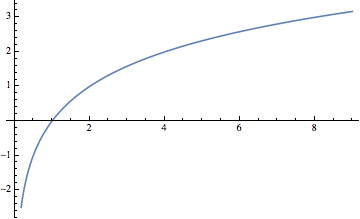
\includegraphics[width=\linewidth]{images/fig-log-2-plot.png}
\end{image}%
\tcblower
\end{figureptx}%
For example, \(\log_2 8 = 3\) because \(2^3 = 8\) and \(\log_21.414\approx 0.5\) because \(2^{0.5}\approx 1.414\). A graph of the function \(f(x)
= \log_2 x\) in \hyperref[x:figure:fig-log-2-plot]{Figure~{\xreffont\ref{x:figure:fig-log-2-plot}}} shows that if \(a < b\), the \(\log_2a < \log_2 b\); that is, when \(x\) increases, \(\log_2 x\) also increases. However, if we move \(x\) from \(2^{10} = 1024\) to \(2^{11} = 2048\), \(\log_2 x\) only increases from 10 to 11. This slow rate of increase of the logarithm function is an important point to remember. An algorithm acting on \(n\) pieces of data that can be executed in \(\log_2{n}\) time units can handle significantly larger sets of data than an algorithm that can be executed in \(n/100\) or  \(\sqrt{n}\) time units. The graph of \(T(n)=\left\lfloor \log_2n\right\rfloor +1\) would show the same behavior.%
\par
A few more properties that we will use in subsequent discussions involving logarithms are summarized in the following theorem.%
\begin{theorem}{Fundamental Properties of Logarithms.}{}{x:theorem:theorem-log-properties}%
\index{Logarithms!Properties}%
Let \(a\) and \(b\) be positive real numbers, and \(r\) a real number.%
\begin{gather}
\log_2 1 = 0\label{x:mrow:eq-log-prop-1}\\
\log_2 a b = \log_2a + \log_2b\label{x:mrow:eq-log-prop-2}\\
\log_2 \frac{a}{b}= \log_2a - \log_2b\label{x:mrow:eq-log-prop-3}\\
\log_2a^r = r \log_2a\label{x:mrow:eq-log-prop-4}\\
2^{\log_2a}= a\label{x:mrow:eq-log-prop-5}
\end{gather}
%
\end{theorem}
\begin{definition}{Logarithms base \(b\).}{x:definition:def-logarithm-general-base}%
\index{Logarithm!General Base}%
\label{g:notation:idm40460008048}%
If \(b > 0\), \(b \neq 1\), then for \(a>0\),%
\begin{equation*}
\log_b a = x\Leftrightarrow b^x= a
\end{equation*}
%
\end{definition}
\begin{theorem}{How logarithms with different bases are related.}{}{x:theorem:theorem-logs-related}%
Let \(b>0\), \(b \neq 1\). Then for all \(a >0\), \(\log_b a = \frac{\log_2a}{\log_2b}\). Therefore, if \(b > 1\), base b logarithms can be computed from base 2 logarithms by dividing by the positive scaling factor \(\log_2b\). If \(b < 1\), this scaling factor is negative.%
\end{theorem}
\begin{proof}{}{g:proof:idm40460003760}
By an analogue of \hyperref[x:mrow:eq-log-prop-5]{({\xreffont\ref{x:mrow:eq-log-prop-5}})}, \(a=b^{\log_b a}\). Therefore, if we take the base 2 logarithm of both sides of this equality we get:%
\begin{equation*}
\log_2 a = \log_2 \left(b^{\log_b a}\right)  \Rightarrow \log_2 a =\log_b a \cdot \log_2 b
\end{equation*}
Finally, divide both sides of the last equation by \(\log_2b\).%
\end{proof}
\begin{note}{}{g:note:idm40459998000}%
\(\log_{2}10 \approx  3.32192\) and \(\log_{2}e \approx 1.4427\).%
\end{note}
\end{subsubsectionptx}
%
%
\typeout{************************************************}
\typeout{Subsubsection 8.4.2.3 }
\typeout{************************************************}
%
\begin{subsubsectionptx}{}{}{}{}{}{g:subsubsection:idm40467754080}
Returning to the binary search algorithm, we can derive the final expression for \(T(n)\) using the properties of logarithms, including that the logarithm function is increasing so that inequalities are maintained when taking logarithms of numbers.%
\par
%
\begin{equation*}
\begin{split}
T(n)= r & \Leftrightarrow 2^{r-1}\leq n < 2^r\\
& \Leftrightarrow  \log_2 2^{r-1} \leq \log_2 n < \log_2 2^r\\
& \Leftrightarrow  r-1 \leq \log_2 n < r\\
& \Leftrightarrow  r-1 = \lfloor \log_2 n\rfloor \\
& \Leftrightarrow  T(n) = r= \left\lfloor \log_2 n\right\rfloor +1
\end{split}
\end{equation*}
%
\par
We can apply several of these properties of logarithms to get an alternate expression for \(T(n)\):%
\begin{equation*}
\begin{split}
\left\lfloor \log_2n\right\rfloor +1 &= \left\lfloor \log_2n+1\right\rfloor \\
& = \left\lfloor \log_2n + \log_22\right\rfloor \\
&  =\text{  }\left\lfloor \log_22n \right\rfloor 
\end{split}
\end{equation*}
%
\par
If the time that was assigned to Step 1 of the binary search algorithm is changed, we wouldn't expect the form of the solution to be very different. If \(T(n)= a + T (\lfloor n/2 \rfloor )\) with \(T(0) = c\), then \(T(n) = c + a \left\lfloor \log_2{2n}\right\rfloor\).%
\par
A further generalization would be to add a coefficient to \(T(\lfloor n/2 \rfloor )\): \(T(n)= a + b T (\lfloor n/2 \rfloor )\) with \(T(0) = c\), where \(a, b, c\in \mathbb{R}\), and \(b\neq 0\) is not quite as simple to derive. First, if we consider values of \(n\) that are powers of 2:%
\begin{equation*}
\begin{array}{c}
T(1) = a + b T(0) = a + b c\\
T(2)=a + b(a+b c) = a + a b +c b^2\\
T(4)=a+b\left(a + a b +c b^2\right) = a + a b + a b^2+ c b^3\\
\vdots \\
T\left(2^r\right) = a + a b + a b^2+\cdots  + a b^r + c b^{r+1}
\end{array}
\end{equation*}
If \(n\) is not a power of 2, by reasoning that is identical to what we used to \hyperref[x:mrow:eq-bin-search-recursion]{({\xreffont\ref{x:mrow:eq-bin-search-recursion}})}  and \hyperref[x:mrow:eq-bin-search-basis]{({\xreffont\ref{x:mrow:eq-bin-search-basis}})},%
\begin{equation*}
T(n) =\sum_{k=0}^r a b^k+ c b^{r+1}
\end{equation*}
where \(r = \left\lfloor \log_2n\right\rfloor\).%
\par
The first term of this expression is a geometric sum, which can be written in closed form. Let \(x\) be that sum:%
\begin{equation*}
\begin{array}{c}
x =a + a b + a b^2+\cdots  + a b^r \\
b x= \textrm{   }a b + a b^2+\cdots  + a b^r + a b^{r+1}
\end{array}
\end{equation*}
We've multiplied each term of \(x\) by \(b\) and aligned the identical terms in \(x\) and \(bx\). Now if we subtract the two equations,%
\begin{equation*}
x - b x = a - a b ^{r+1} \Rightarrow x(1-b) = a\left(1-b^{r+1}\right)
\end{equation*}
Therefore, \(x = a\frac{b^{r+1}-1}{b-1}\).%
\par
A closed form expression for \(T(n)\) is%
\begin{equation*}
T(n) = a\frac{b^{r+1}-1}{b-1} +\text{  }c b^{r+1}\text{  }\text{where}\text{  }r = \left\lfloor \log_2n\right\rfloor \text{  }
\end{equation*}
%
\end{subsubsectionptx}
\end{subsectionptx}
%
%
\typeout{************************************************}
\typeout{Subsection 8.4.3 Analysis of Bubble Sort and Merge Sort}
\typeout{************************************************}
%
\begin{subsectionptx}{Analysis of Bubble Sort and Merge Sort}{}{Analysis of Bubble Sort and Merge Sort}{}{}{x:subsection:ss-bubblesort-analysis}
\index{Bubble Sort}%
\index{Merge Sort}%
The efficiency of any search algorithm such as the binary search relies on fact that the search list is sorted according to a key value and that the search is based on the key value. There are several methods for sorting a list. One example is the bubble sort. You might be familiar with this one since it is a popular ``first sorting algorithm.'' A time analysis of the algorithm shows that if \(B(n)\) is the worst-case time needed to complete the bubble sort on \(n\) items, then \(B(n) =(n-1) + B(n-1)\) and \(B(1) = 0\). The solution of this relation is a quadratic function \(B(n) =\frac{1}{2}\left(n^2-n\right)\). The growth rate of a quadratic function such as this one is controlled by its squared term. Any other terms are dwarfed by it as \(n\) gets large. For the bubble sort, this means that if we double the size of the list that we are to sort, \(n\) changes to \(2n\) and so \(n^2\) becomes \(4n^2\) . Therefore, the time needed to do a bubble sort is quadrupled. One alternative to bubble sort is the merge sort. Here is a simple version of this algorithm for sorting \(F=\{r(1), r(2), \ldots , r(n)\}\), \(n \geq  1\). If \(n
= 1\), the list is sorted trivially. If \(n\geq  2\) then:%
\par
%
\begin{enumerate}[label=(\arabic*)]
\item{}Divide \(F\) into \(F_1= \{r(1), \ldots , r(\lfloor n/2\rfloor )\}\) and \(F_2= \{r(\lfloor n/2\rfloor +1), \ldots ,r(n)\}\).%
\item{}Sort \(F_1\) and \(F_2\) using a merge sort.%
\item{}Merge the sorted lists \(F_1\) and \(F_2\) into one sorted list. If the sort is to be done in descending order of key values, you continue to choose the higher key value from the fronts of \(F_1\) and \(F_2\) and place them in the back of \(F\).%
\end{enumerate}
%
\par
Note that \(F_1\) will always have \(\lfloor n/2\rfloor\) items and \(F_2\) will have \(\lceil n/2\rceil\) items; thus, if \(n\) is odd, \(F_2\) gets one more item than \(F_1\). We will assume that the time required to perform Step 1 of the algorithm is insignificant compared to the other steps; therefore, we will assign a time value of zero to this step. Step 3 requires roughly \(n\) comparisons and \(n\) movements of items from \(F_1\) and \(F_2\) to \(F\); thus, its time is proportional to \(n\). For this reason, we will assume that Step 3 takes \(n\) time units. Since Step 2 requires \(T(\lfloor n/2\rfloor ) + T(\lceil n/2\rceil )\) time units,%
\begin{gather}
T(n) = n + T(\lfloor n/2\rfloor ) + T(\lceil n/2\rceil )\label{x:mrow:eq-bubble-r}
\end{gather}
with the initial condition%
\begin{gather}
T(1) = 0\label{x:mrow:eq-bubble-b}
\end{gather}
%
\par
Instead of an exact solution of these equations, we will be content with an estimate for \(T(n)\).  First, consider the case of \(n=2^r\), \(r \geq 1\):%
\begin{equation*}
\begin{array}{c}
T\left(2^1\right)= T(2) = 2 +T(1)+T(1)= 2 = 1\cdot  2\\
T\left(2^2\right) = T(4)=4+\text{  }T(2)+T(2)=8 = 2\cdot 4\\
T\left(2^3\right) =T(8)=8 + T(4)+T(4) =24=3\cdot 8\\
\vdots \\
T\left(2^r\right)=r 2^r= 2^r \log_2 2^r
\end{array}
\end{equation*}
%
\par
Thus, if \(n\) is a power of 2, \(T(n) = n \log_2 n\). Now if, for some \(r \geq  2\), \(2^{r-1}\leq n\leq 2^r\), then \((r-1)2^{r-1}\leq
T(n) < r 2^r\). This can be proved by induction on \(r\). As \(n\) increases from \(2^{r-1}\) to \(2^r\), \(T(n)\) increases from \((r-1)2^{r-1}\)to \(r 2^r\) and is slightly larger than \(\left\lfloor n \log_2n\right\rfloor\). The discrepancy is small enough so that \(T_e(n)=\left\lfloor n \log
_2n\right\rfloor\) can be considered a solution of \hyperref[x:mrow:eq-bubble-r]{({\xreffont\ref{x:mrow:eq-bubble-r}})} and \hyperref[x:mrow:eq-bubble-b]{({\xreffont\ref{x:mrow:eq-bubble-b}})} for the purposes of comparing the merge sort with other algorithms. \hyperref[x:table:table-sort-analysis]{Table~{\xreffont\ref{x:table:table-sort-analysis}}} compares \(B(n)\) with \(T_e(n)\) for selected values of \(n\).%
\begin{tableptx}{\textbf{Comparison of Times for Bubble Sort and Merge Sort}}{x:table:table-sort-analysis}{}%
\centering
{\tabularfont%
\begin{tabular}{ccc}\hrulethick
n&\(B(n)\)&\(T_e(n)\)\tabularnewline[0pt]
10&45&34\tabularnewline[0pt]
50&1225&283\tabularnewline[0pt]
100&4950&665\tabularnewline[0pt]
500&124750&4483\tabularnewline[0pt]
1000&499500&9966
\end{tabular}
}%
\end{tableptx}%
\end{subsectionptx}
%
%
\typeout{************************************************}
\typeout{Subsection 8.4.4 Derangements}
\typeout{************************************************}
%
\begin{subsectionptx}{Derangements}{}{Derangements}{}{}{x:subsection:ss-derangements}
\index{Derangement}%
A derangement is a permutation on a set that has no ``fixed points''.  Here is a formal definition:%
\begin{definition}{Derangement.}{x:definition:def-derangement}%
A derangement of a nonempty set \(A\) is a permutation of \(A\) (i.e., a bijection from \(A\) into \(A\)) such that \(f(a)\neq a\) for all \(a \in  A\).%
\end{definition}
If \(A = \{1, 2, . . . , n\}\), an interesting question might be ``How many derangements are there of \(A\)?''  We know that our answer is bounded above by \(n!\). We can also expect our answer to be quite a bit smaller than \(n!\) since \(n\) is the image of itself for \((n-1)!\) of the permutations of \(A\).%
\par
Let \(D(n)\) be the number of derangements of \(\{1, 2, . . . , n\}\). Our answer will come from discovering a recurrence relation on \(D\). Suppose that \(n \geq  3\). If we are to construct a derangement of \(\{1, 2, \dots , n\}\), \(f\), then \(f(n) = k \neq n\). Thus, the image of \(n\) can be selected in \(n-1\) different ways. No matter which of the \(n -1\) choices we make, we can complete the definition of \(f\) in one of two ways. First, we can decide to make \(f(k) = n\), leaving \(D(n -2)\) ways of completing the definition of \(f\), since \(f\) will be a derangement of \(\{1, 2, \dots ,n\} - \{n, k\}\). Second, if we decide to select \(f(k)\neq  n\), each of the \(D(n - 1)\) derangements of \(\{1, 2,\dots ,n-1\}\) can be used to define \(f\). If \(g\) is a derangement of \(\{1, 2, \dots , n-1\}\) such that \(g(p) = k\), then define f by%
\begin{equation*}
f(j)=\left\{
\begin{array}{cc}
n & \textrm{ if } j = p \\
k & \textrm{ if } j = n \\
g(j) & \textrm{ otherwise } \\
\end{array}
\right.
\end{equation*}
%
\par
Note that with our second construction of \(f\), \(f(f(n)) = f(k) \neq  n\), while in the first construction, \(f(f(n)) = f(k) = n\). Therefore, no derangement of \(\{1, 2, . . . , n\}\) with \(f(n) = k\) can be constructed by both methods.%
\par
To recap our result, we see that \(f\) is determined by first choosing one of \(n - 1\) images of \(n\) and then constructing the remainder of \(f\) in one of \(D(n - 2) + D(n -1)\) ways. Therefore,%
\begin{gather}
D(n) = (n - 1) (D(n - 2) + D(n - 1))\label{g:mrow:idm40459912128}
\end{gather}
%
\par
This homogeneous second-order linear relation with variable coefficients, together with the initial conditions \(D(1) = 0\) and \(D(2) = 1\), completely defines \(D\). Instead of deriving a solution of this relation by analytical methods, we will give an empirical derivation of an approximation of \(D(n)\). Since the derangements of \(\{1,2 . . . , n\}\) are drawn from a pool of \(n!\) permutations, we will see what percentage of these permutations are derangements by listing the values of \(n!\), \(D(n)\), and \(\frac{D(n)}{n!}\).  The results we observe will indicate that as \(n\) grows, \(\frac{D(n)}{n!}\) hardly changes at all. If this quotient is computed to eight decimal places, for \(n \geq  12\), \(D(n)/n!
= 0.36787944\). The reciprocal of this number, which \(D(n)/n!\) seems to be tending toward, is, to eight places, 2.7182818. This number appears in so many places in mathematics that it has its own name, \(e\). An approximate solution of our recurrence relation on \(D\) is then \(D(n)\approx \frac{n!}{e}\).%
\begin{sageinput}
def D(n):
    if n<=2:
        return n-1
    else:
        return (n-1)*(D(n-2)+D(n-1))

list(map(lambda k:[k,D(k),(D(k)/factorial(k)).n(digits=8)],range(1,16)))
\end{sageinput}
\begin{sageoutput}
[[1, 0, 0.00000000],
 [2, 1, 0.50000000],
 [3, 2, 0.33333333],
 [4, 9, 0.37500000],
 [5, 44, 0.36666667],
 [6, 265, 0.36805556],
 [7, 1854, 0.36785714],
 [8, 14833, 0.36788194],
 [9, 133496, 0.36787919],
 [10, 1334961, 0.36787946],
 [11, 14684570, 0.36787944],
 [12, 176214841, 0.36787944],
 [13, 2290792932, 0.36787944],
 [14, 32071101049, 0.36787944],
 [15, 481066515734, 0.36787944]]
\end{sageoutput}
\end{subsectionptx}
%
%
\typeout{************************************************}
\typeout{Exercises 8.4.5 Exercises}
\typeout{************************************************}
%
\begin{exercises-subsection}{Exercises}{}{Exercises}{}{}{x:exercises:exercises-8-4}
\begin{divisionexercise}{1}{}{}{g:exercise:idm40459901904}%
Solve the following recurrence relations. Indicate whether your solution is an improvement over iteration.%
\par
%
\begin{enumerate}[label=(\alph*)]
\item{}\(n S(n) - S(n - 1) = 0\), \(S(0) = 1\).%
\item{}\(T(k) + 3k T(k - 1) = 0\), \(T(0) = 1\).%
\item{}\(U(k) -\frac{k-1}{k}U(k - 1) = 0\), \(k \geq  2\), \(U(1) = 1\).%
\end{enumerate}
%
\end{divisionexercise}%
\begin{divisionexercise}{2}{}{}{g:exercise:idm40459892880}%
Prove that if \(n \geq 0\), \(\lfloor n/2\rfloor +\lceil n/2\rceil = n\). (Hint: Consider the cases of \(n\) odd and \(n\) even separately.)%
\end{divisionexercise}%
\begin{divisionexercise}{3}{}{}{g:exercise:idm40459890608}%
Solve as completely as possible:%
\par
%
\begin{enumerate}[label=(\alph*)]
\item{}\(T(n) = 3 + T(\lfloor n/2\rfloor )\), \(T(0) = 0\).%
\item{}\(T(n) = 1 + \frac{1}{2}T(\lfloor n/2\rfloor )\), \(T(0) = 2\).%
\item{}\(V(n) = 1 + V\lfloor n/8\rfloor )\), \(V(0) = 0\). (Hint: Write \(n\) in octal form.)%
\end{enumerate}
%
\end{divisionexercise}%
\begin{divisionexercise}{4}{}{}{g:exercise:idm40459882384}%
Prove by induction that if \(T(n)= 1 + T (\lfloor n/2 \rfloor )\), \(T(0) = 0\), and \(2^{r-1}\leq n < 2^r\) , \(r \geq  1\), then \(T(n) = r\).%
\par\smallskip%
\noindent\textbf{\blocktitlefont Hint}.\hypertarget{g:hint:idm40459881776}{}\quad{}Prove by induction on \(r\).%
\end{divisionexercise}%
\begin{divisionexercise}{5}{}{}{g:exercise:idm40459878928}%
Use the substitution \(S(n) = T(n+1)/T(n)\)  to solve \(T(n)T(n-2)=T(n-1)^2\) for \(n \geq  2\), with \(T(0) = 1\), \(T(1) = 6\), and \(T(n) \geq  0\).%
\end{divisionexercise}%
\begin{divisionexercise}{6}{}{}{g:exercise:idm40459875440}%
Use the substitution \(G(n) =T(n)^2\) to solve \(T(n)^2-T(n-1)^2=1\) for \(n \geq  1\), with \(T(0) = 10\).%
\end{divisionexercise}%
\begin{divisionexercise}{7}{}{}{g:exercise:idm40459870592}%
Solve as completely as possible:%
\par
%
\begin{enumerate}[label=(\alph*)]
\item{}\(Q(n)=1+Q\left(\left\lfloor \sqrt{n}\right\rfloor \right)\), \(n \geq  2\), \(Q(1) = 0\).%
\item{}\(R(n)=n +R(\lfloor n/2\rfloor )\), \(n \geq  1\), \(R(0) = 0\).%
\end{enumerate}
%
\end{divisionexercise}%
\begin{divisionexercise}{8}{}{}{g:exercise:idm40459859136}%
Suppose Step 1 of the merge sort algorithm did take a significant amount of time. Assume it takes 0.1 time unit, independent of the value of \(n\).%
\par
%
\begin{enumerate}[label=(\alph*)]
\item{}Write out a new recurrence relation for \(T(n)\) that takes this factor into account.%
\item{}Solve for \(T\left(2^r\right)\), \(r \geq  0\).%
\item{}Assuming the solution for powers of 2 is a good estimate for all \(n\), compare your result to the solution in the text. As gets large, is there really much difference?%
\end{enumerate}
%
\end{divisionexercise}%
\end{exercises-subsection}
\end{sectionptx}
%
%
\typeout{************************************************}
\typeout{Section 8.5 Generating Functions}
\typeout{************************************************}
%
\begin{sectionptx}{Generating Functions}{}{Generating Functions}{}{}{x:section:s-generating-functions}
\index{Generating Functions}%
\begin{introduction}{}%
This section contains an introduction to the topic of generating functions and how they are used to solve recurrence relations, among other problems. Methods that employ generating functions are based on the concept that you can take a problem involving sequences and translate it into a problem involving generating functions. Once you've solved the new problem, a translation back to sequences gives you a solution of the original problem.%
\par
This section covers:%
\begin{enumerate}[label=(\arabic*)]
\item{}The definition of a generating function.%
\item{}Solution of a recurrence relation using generating functions to identify the skills needed to use generating functions.%
\item{}An introduction and\slash{}or review of the skills identified in point 2.%
\item{}Some applications of generating functions.%
\end{enumerate}
%
\end{introduction}%
%
%
\typeout{************************************************}
\typeout{Subsection 8.5.1 Definition}
\typeout{************************************************}
%
\begin{subsectionptx}{Definition}{}{Definition}{}{}{x:subsection:ss-what-is-a-generating-function}
\begin{definition}{Generating Function of a Sequence.}{x:definition:def-generating-function}%
\index{Generating Function}%
\label{g:notation:idm40459843200}%
The generating function of a sequence \(S\) with terms \(S_0,S_1 ,S_2, \dots \),  is the infinite sum%
\begin{equation*}
G(S;z)=\sum_{n=0}^{\infty} S_n z^n=S_0+S_1 z+S_2 z^2+S_3 z^3+\cdots
\end{equation*}
The domain and codomain of generating functions will not be of any concern to us since we will only be performing algebraic operations on them.%
\end{definition}
\begin{example}{First Examples.}{x:example:ex-first-gf-examples}%
%
\begin{enumerate}[label=(\alph*)]
\item{}If \(S_n = 3^n\),\(n \geq  0\), then%
\begin{equation*}
\begin{split}
G(S;z) &= 1 + 3z + 9z^2 + 27z^3 +\cdots \\
& =\sum_{n=0}^{\infty} 3^n z^n\\	
&=\sum_{n=0}^{\infty} (3 z)^n\\
\end{split}
\end{equation*}
We can get a closed form expression for \(G(S;z)\) by observing that \(G(S;z) - 3z G(S;z) = 1\). Therefore, \(G(S;z) =\frac{1}{1-3 z}\).%
\item{}Finite sequences have generating functions. For example, the sequence of binomial coefficients \(\binom{n}{0} \), \(\binom{n}{1} \), \(\ldots\),\(\binom{n}{n} \), \(n \geq  1\) has generating function%
\begin{equation*}
\begin{split}
G(\binom{n}{\cdot}; z) & = \binom{n}{0}  + \binom{n}{1} z +\cdots  + \binom{n}{n} z^n\\
& = \sum_{k=0}^{\infty} \binom{n}{k}  z^k\\
&=(1+z)^n\\
\end{split}
\end{equation*}
by application of the binomial formula.%
\item{}If \(Q(n) = n^2\), \(G(Q;z)=\sum_{n=0}^{\infty} n^2 z^n=\sum_{k=0}^{\infty} k^2 z^k\). Note that the index that is used in the summation has no significance. Also, note that the lower limit of the summation could start at 1 since \(Q(0)=0\).%
\end{enumerate}
%
\end{example}
\end{subsectionptx}
%
%
\typeout{************************************************}
\typeout{Subsection 8.5.2 Solution of a Recurrence Relation Using Generating Functions}
\typeout{************************************************}
%
\begin{subsectionptx}{Solution of a Recurrence Relation Using Generating Functions}{}{Solution of a Recurrence Relation Using Generating Functions}{}{}{x:subsection:ss-solution-of-rr-using-generating-functions}
We illustrate the use of generating functions by solving \(S(n) - 2S(n - 1) - 3S(n - 2) = 0\), \(n \geq  2\), with \(S(0) = 3\) and \(S(1) = 1\).%
\par
%
\begin{enumerate}[label=(\arabic*)]
\item{}Translate the recurrence relation into an equation about generating functions.%
\par
Let \(V(n) = S(n) - 2S (n - 1) - 3S (n - 2)\), \(n \geq  2\), with \(V(0) = 0\) and \(V(1) = 0\). Therefore,%
\begin{equation*}
G(V;z) = 0 + 0z +\sum_{n=2}^{\infty}  (S(n) - 2S (n - 1) - 3S (n - 2)) z^n= 0
\end{equation*}
%
\item{}Solve for the generating function of the unknown sequence, \(G(S;z) = \sum_{n=0}^{\infty} S_n z^n\).%
\begin{equation*}
\begin{split}
0 & =\sum_{n=2}^{\infty}  {(S(n) - 2S (n - 1) - 3 S (n - 2)) z^n}\\
& =\sum_{n=2}^{\infty} {S(n) z^n-2} \left(\sum_{n=2}^{\infty
} S(n-1) z^n\right)-3\left(\sum_{n=2}^{\infty} S(n-2) z^n\right)
\end{split}
\end{equation*}
%
\par
Close examination of the three sums above shows:%
\par
%
\begin{enumerate}[label=(\alph*)]
\item{}%
\begin{equation*}
\begin{split}
\sum_{n=2}^{\infty} S_n z^n &=\sum_{n=0}^{\infty} S_n z^n - S(0)-S(1)z\\
&= G(S;z)-3-z
\end{split}
\end{equation*}
since \(S(0)=3\) and \(S(1)=1\).%
\item{}%
\begin{equation*}
\begin{split}
\sum_{n=2}^{\infty} S(n-1) z^n &=z\left(\sum_{n=2}^{\infty} S(n-1) z^{n-1}\right)\\
& =z\left(\sum_{n=1}^{\infty} S(n) z^n\right)\\
& = z\left(\sum_{n=0}^{\infty} S(n) z^n-S(0)\right)\\
&= z(G(S;z)-3)
\end{split}
\end{equation*}
%
\item{}%
\begin{equation*}
\begin{split}
\sum_{n=2}^{\infty} S(n-2) z^n  & = z^2\left(\sum_{n=2}^{\infty} S(n-2) z^{n-2}\right)\\
& =z^2G(S;z)
\end{split}
\end{equation*}
%
\par
Therefore,%
\begin{equation*}
\begin{split}
&(G(S;z)-3-z)-2z(G(S;z)-3)-3z^2G(S;z)=0\\
& \Rightarrow G(S;z)-2z G(S;z)-3z^2G(S;z)=3 - 5z\\
&\Rightarrow G(S;z)=\frac{3-5z}{1-2z-3z^2}
\end{split}
\end{equation*}
%
\end{enumerate}
%
\item{}Determine the sequence whose generating function is the one we got in Step 2.%
\par
For our example, we need to know one general fact about the closed form expression of an exponential sequence (a proof will be given later):%
\begin{gather}
T(n)=b a^n ,n\geq 0 \Leftrightarrow G(T;z)=\frac{b}{1-a z} \label{x:mrow:gf-of-exp}
\end{gather}
%
\par
Now, in order to recognize \(S\) in our example, we must write our closed form expression for \(G(S;z)\) as a sum of terms like \(G(T;z)\) above. Note that the denominator of \(G(S;z)\) can be factored:%
\begin{equation*}
G(S;z)=\frac{3-5z}{1-2z-3z^2} =\frac{3-5z}{(1-3z)(1+z)}
\end{equation*}
If you look at this last expression for \(G(S;z)\) closely, you can imagine how it could be the result of addition of two fractions,%
\begin{gather}
\frac{3-5z}{(1-3z)(1+z)} = \frac{A}{1-3z}+ \frac{B}{1+z}\label{x:mrow:eq-pf}
\end{gather}
where \(A\) and \(B\) are two real numbers that must be determined. Starting on the right of \hyperref[x:mrow:eq-pf]{({\xreffont\ref{x:mrow:eq-pf}})}, it should be clear that the sum, for any \(A\) and \(B\), would look like the left-hand side. The process of finding values of \(A\) and \(B\) that make \hyperref[x:mrow:eq-pf]{({\xreffont\ref{x:mrow:eq-pf}})} true is called the \terminology{partial fractions decomposition} of the left-hand side:%
\begin{equation*}
\begin{split}
\frac{A}{1-3z}+ \frac{B}{1+z} &=\frac{A(1+z)}{(1-3z)(1+z)}+ \frac{B(1-3z)}{(1-3z)(1+z)}\\
& =\frac{(A+B)+(A-3B)z}{(1-3z)(1+z)}
\end{split}
\end{equation*}
%
\par
Therefore,%
\begin{equation*}
\left\{
\begin{array}{c}
A+B=3 \\
A-3B=-5 \\
\end{array}
\right\}\Rightarrow \left\{
\begin{array}{c}
A=1 \\
B=2 \\
\end{array}
\right\}
\end{equation*}
and%
\begin{equation*}
G(S;z)= \frac{1}{1-3z}+ \frac{2}{1+z}
\end{equation*}
%
\par
We can apply \hyperref[x:mrow:gf-of-exp]{({\xreffont\ref{x:mrow:gf-of-exp}})} to each term of \(G(S;z)\):%
\par
%
\begin{itemize}[label=\textbullet]
\item{}\(\frac{1}{1-3z}\) is the generating function for \(S_1(n)=1\cdot  3^n= 3^n\)%
\item{}\(\frac{2}{1+z}\) is the generating function for \(S_2(n)=2(-1)^n\).%
\end{itemize}
%
\par
Therefore, \(S(n)=3^n+ 2(-1)^n\).%
\end{enumerate}
%
\par
From this example, we see that there are several skills that must be mastered in order to work with generating functions. You must be able to:%
\par
%
\begin{enumerate}[label=(\alph*)]
\item{}Manipulate summation expressions and their indices (in Step 2).%
\item{}Solve algebraic equations and manipulate algebraic expressions, including partial function decompositions (Steps 2 and 3).%
\item{}Identify sequences with their generating functions (Steps 1 and 3).%
\end{enumerate}
%
\par
We will concentrate on the last skill first, a proficiency in the other skills is a product of doing as many exercises and reading as many examples as possible.%
\par
First, we will identify the operations on sequences and on generating functions.%
\end{subsectionptx}
%
%
\typeout{************************************************}
\typeout{Subsection 8.5.3 Operations on Sequences}
\typeout{************************************************}
%
\begin{subsectionptx}{Operations on Sequences}{}{Operations on Sequences}{}{}{x:subsection:ops-on-sequences}
\begin{definition}{Operations on Sequences.}{g:definition:idm40459795952}%
\index{Sequences!Operations on}%
\label{g:notation:idm40459794768}%
\label{g:notation:idm40459793792}%
\label{g:notation:idm40459792816}%
Let \(S\) and \(T\) be sequences of numbers and let \(c\) be a real number. Define the sum \(S + T\), the scalar product \(c S\), the product \(S T\), the convolution \(S*T\), the pop operation \(S\uparrow\) (read ``\(S\) pop''), and the push operation \(S\downarrow\) (read ``\(S\) push'') term-wise for \(k \geq  0\) by%
\begin{gather}
(S + T)(k) = S(k) + T(k)\label{x:mrow:seq-op-add}
\end{gather}
%
\begin{gather}
(c S)(k) = c S(k)\label{x:mrow:seq-op-sc-mult}
\end{gather}
%
\begin{gather}
(S \cdot T)(k) = S(k)T(k)\label{x:mrow:seq-op-mult}
\end{gather}
%
\begin{gather}
(S*T)(k) = \sum_{j=0}^k S(j) T(k-j)\label{x:mrow:seq-op-convolve}
\end{gather}
%
\begin{gather}
(S\uparrow )(k) = S(k+1)\label{x:mrow:seq-op-pop}
\end{gather}
%
\begin{align}
(S\downarrow )(k)=\left\{
\begin{array}{cc} 
0 & \textrm{ if } k=0 \\
S(k-1) & \textrm{ if } k>0 
\end{array}\right.\label{x:mrow:seq-op-push}
\end{align}
%
\end{definition}
If one imagines a sequence to be a matrix with one row and an infinite number of columns, \(S + T\) and \(c S\) are exactly as in matrix addition and scalar multiplication. There is no obvious similarity between the other operations and matrix operations.%
\par
The pop and push operations can be understood by imagining a sequence to be an infinite stack of numbers with \(S(0)\) at the top, \(S(1)\) next, etc., as in \hyperref[x:figure:fig-pop-push]{Figure~{\xreffont\ref{x:figure:fig-pop-push}}}a. The sequence \(S\uparrow\) is obtained by ``popping'' S(0) from the stack, leaving a stack as in \hyperref[x:figure:fig-pop-push]{Figure~{\xreffont\ref{x:figure:fig-pop-push}}}b, with S(1) at the top, S(2) next, etc. The sequence \(S\downarrow\) is obtained by placing a zero at the top of the stack, resulting in a stack as in \hyperref[x:figure:fig-pop-push]{Figure~{\xreffont\ref{x:figure:fig-pop-push}}}c. Keep these figures in mind when we discuss the pop and push operations.%
\begin{figureptx}{Stack interpretation of pop and push operation}{x:figure:fig-pop-push}{}%
\begin{image}{0}{1}{0}%
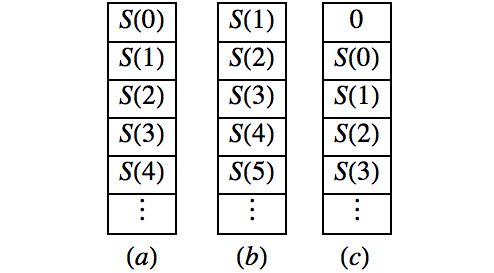
\includegraphics[width=\linewidth]{images/fig-pop-push.png}
\end{image}%
\tcblower
\end{figureptx}%
\begin{example}{Some Sequence Operations.}{x:example:ex-some-sequence-operations}%
If \(S(n) = n\), \(T(n) = n^2\), \(U(n) = 2^n\), and \(R(n) =n 2^n\):%
\par
%
\begin{enumerate}[label=(\alph*)]
\item{}\((S + T)(n) = n + n^2\)%
\item{}\((U + R)(n) = 2^n+ n 2^n= (1+n)2^n\)%
\item{}\((2 U)(n) = 2\cdot 2^n= 2^{n+1}\)%
\item{}\(\left(\frac{1}{2}R\right)(n)= \frac{1}{2}n 2^n= n 2^{n-1}\)%
\item{}\((S\cdot T)(n) = n n^2 = n^3\)%
\item{}\((S*T)(n)= \sum_{j=0}^n S(j) T(n-j)= \sum_{j=0}^n j (n-j)^2\\
\\
\quad \quad =\sum_{j=0}^n \left( j n^2-2 n j^2 + j^3\right)\\
\\
\quad \quad = n^2\sum_{j=0}^n j-2n \sum_{j=0}^n j^2 + \sum_{j=0}^n j ^3\\
\\
\quad \quad =n^{2 }\left(\frac{n (n+1)}{2}\right)- 2n\left(\frac{(2n+1)(n+1)n}{6}\right)+\frac{1}{4} n^2 (n+1)^2\\
\\
\quad \quad = \frac{n^2(n+1)(n-1)}{12}\)%
\item{}\((U*U)(n) =\sum_{j=0}^n U(j) U(n-j)\\
\\
\quad \quad =\sum_{j=0}^n 2^j 2^{n-j}\\
\\
\quad \quad = (n+1)2^n\)%
\item{}\((S\uparrow )(n)=n+1\)%
\item{}\((S\downarrow )(n)=\max (0,n-1)\)%
\item{}\(((S\downarrow )\downarrow )(n)= \max (0, n - 2)\)%
\item{}\((U\downarrow )(n)=\left\{
\begin{array}{cc}
2^{n-1} & \textrm{ if } n>0 \\
0 & \textrm{ if } n=0 \\
\end{array}
\right.\)%
\item{}\(((U\downarrow )\uparrow )(n)=(U\downarrow )(n+1)= 2^n= U(n)\)%
\item{}\(((U\uparrow )\downarrow ) (n)=\left\{
\begin{array}{cc}
0 & \textrm{ if } n = 0 \\
U(n) & \textrm{ if } n>0 \\
\end{array}
\right.\)%
\end{enumerate}
%
\end{example}
Note that \((U\downarrow )\uparrow \neq (U\uparrow )\downarrow\).%
\begin{definition}{Multiple Pop and Push.}{x:definition:def-multiple-pop-and-push}%
\index{Multiple Pop and Push}%
\label{g:notation:idm40459758528}%
\label{g:notation:idm40459757984}%
If S is a sequence of numbers and \(p\) a positive integer greater than 1, define%
\begin{equation*}
S\uparrow p = (S\uparrow (p - 1))\uparrow \quad\textrm{ if }p \geq  2 \textrm{ and }S\uparrow 1 = S\uparrow
\end{equation*}
Similarly, define%
\begin{equation*}
S\downarrow p = (S\downarrow (p - 1))\downarrow \quad\textrm{ if } p \geq  2\textrm{ and }S\downarrow 1 = S\downarrow
\end{equation*}
%
\end{definition}
In general, \((S \uparrow p)(k) = S(k+p),\) and%
\begin{equation*}
(S\downarrow p)(k)=\left\{
\begin{array}{cc}
0 & \textrm{ if } k < p \\
S(k-p) & \textrm{ if } k\geq p \\
\end{array}
\right.
\end{equation*}
%
\end{subsectionptx}
%
%
\typeout{************************************************}
\typeout{Subsection 8.5.4 Operations on Generating Functions}
\typeout{************************************************}
%
\begin{subsectionptx}{Operations on Generating Functions}{}{Operations on Generating Functions}{}{}{x:subsection:sss-operations-on-generating-functions}
\index{Generating Functions!Operations on}%
\begin{definition}{Operations on Generating Functions.}{g:definition:idm40459751344}%
\index{Generating Functions!Operations on}%
If  \(G(z)=\sum_{k=0}^{\infty} a_k z^k\) and \(H(z) =\sum_{k=0}^{\infty} b_k z^k\) are generating functions and \(c\) is a real number, then the sum \(G + H\), scalar product \(c G\), product \(G H\), and monomial product \(z^p G\), \(p \geq  1\) are generating functions, where%
\begin{gather}
(G + H)(z)=\sum_{k=0}^{\infty} \left(a_k+b_k\right) z^k\label{x:mrow:gf-sum}\\
(c G)(z)=\sum_{k=0}^{\infty} c a_k z^k\label{x:mrow:gf-scalarmult}\\
(G H)(z) = \sum_{k=0}^{\infty} c z^k \textrm{ where } c_k= \sum_{j=0}^k a_jb_{k-j}\label{x:mrow:gf-product}\\
\left(z^p G\right)(z) = z^p\sum_{k=0}^{\infty} a_k z^k=\sum_{k=0}^{\infty} a_k z^{k+p} = \sum_{n=p}^{\infty} a_{n-p} z^n\label{x:mrow:gf-shift}
\end{gather}
%
\par
The last sum is obtained by substituting \(n - p\) for \(k\) in the previous sum.%
\end{definition}
\begin{example}{Some operations on generating functions.}{x:example:ex-some-gf-operations}%
If \(D(z) =\sum_{k=0}^{\infty} kz^k\) and \(H(z) =\sum_{k=0}^{\infty} 2^k z^k\) then%
\begin{equation*}
(D + H)(z) =\sum_{k=0}^{\infty} \left(k+2^k\right) z^k
\end{equation*}
%
\begin{equation*}
(2H)(z)= \sum_{k=0}^{\infty} 2\cdot 2^kz^k =\sum_{k=0}^{\infty} 2^{k+1}z^k
\end{equation*}
%
\begin{equation*}
\begin{split}
(z D)(z) &= z\sum_{k=0}^{\infty} kz^k= \sum_{k=0}^{\infty} kz^{k+1}\\
&= \sum_{k=1}^{\infty} (k-1) z^k  = D(z)- \sum_{k=1}^{\infty} z^k\\
\end{split}
\end{equation*}
%
\begin{equation*}
(D H)(z)=\sum_{k=0}^{\infty} \left(\sum_{j=0}^k j 2^{k-j}\right)z^k
\end{equation*}
%
\begin{equation*}
(H H)(z)= \sum_{k=0}^{\infty} \left(\sum_{j=0}^k 2^j2^{k-j}\right) z^k=\sum_{k=0}^{\infty} (k+1)2^k z^k
\end{equation*}
%
\par
Note: \(D(z) = G(S;z)\), and \(H(z) = G(U;z)\) from \hyperref[x:example:ex-some-sequence-operations]{Example~5}.%
\end{example}
Now we establish the connection between the operations on sequences and generating functions. Let \(S\) and \(T\) be sequences and let \(c\) be a real number.%
\begin{gather}
G(S+T;z)=G(S;z)+G(T;z)\label{x:mrow:gf-ops-1}\\
G(cS;z)=c G(S;z)\label{x:mrow:gf-ops-2}\\
G(S*T;z)=G(S;z) G(T;z)\label{x:mrow:gf-ops-3}\\
G(S\uparrow ;z)=(G(S;z)-S(0))/z\label{x:mrow:gf-ops-4}\\
G(S\downarrow ;z)=z G(S;z)\label{x:mrow:gf-ops-5}
\end{gather}
%
\par
In words, \hyperref[x:mrow:gf-ops-1]{({\xreffont\ref{x:mrow:gf-ops-1}})} says that the generating function of the sum of two sequences equals the sum of the generating functions of those sequences. Take the time to write out the other four identities in your own words. From the previous examples, these identities should be fairly obvious, with the possible exception of the last two. We will prove \hyperref[x:mrow:gf-ops-4]{({\xreffont\ref{x:mrow:gf-ops-4}})} as part of the next theorem and leave the proof of \hyperref[x:mrow:gf-ops-5]{({\xreffont\ref{x:mrow:gf-ops-5}})} to the interested reader. Note that there is no operation on generating functions that is related to sequence multiplication; that is, \(G(S\cdot T;z)\) cannot be simplified.%
\begin{theorem}{Generating functions related to Pop and Push.}{}{x:theorem:gf-of-pop-push}%
If \(p > 1\),%
\par
%
\begin{enumerate}[label=(\alph*)]
\item{}\(G(S\uparrow p;z) = \left(G(S;z) -\left.\sum_{k=0}^{p-1} S(k) z^k\right)/z^k\right.\)%
\item{}\(G(S\downarrow p;z) = z^p G(S;z)\).%
\end{enumerate}
%
\end{theorem}
\begin{proof}{}{g:proof:idm40459727440}
We prove (a)  by induction and leave the proof of (b) to the reader.%
\par
Basis:%
\begin{equation*}
\begin{split}
G(S\uparrow;z) &= \sum_{k=0}^{\infty} S(k+1) z^k\\
& =\sum_{k=1}^{\infty} S(k) z^{k-1}\\
& =\left.\left(\sum_{k=1}^{\infty} S(k) z^k\right)\right/z\\ 		
& =\left.\left(S(0)+\sum_{k=1}^{\infty} S(k) z^k-S(0)\right)\right/z\\
& =(G(S;z)-S(0))/z
\end{split}
\end{equation*}
Therefore, part (a) is true for \(p=1\).%
\par
Induction: Suppose that for some \(p\geq 1\), the statement in part (a) is true:%
\begin{equation*}
\begin{split}
G(S\uparrow (p+1);z) &= G((S\uparrow p)\uparrow ;z)\\
& = (G(S\uparrow p ;z)-(S\uparrow p)(0))/z \textrm{ by the basis}\\
& = \frac{\frac{\left(G(S;z)-\sum_{k=0}^{p-1} S(k) z^k\right)}{z^p}-S(p)}{z}
\end{split}
\end{equation*}
by the induction hypothesis. Now write \(S(p)\) in the last expression above as \(\left(S(p)z^p \right)/z^p\) so that it fits into the finite summation:%
\begin{equation*}
\begin{split}
G(S\uparrow (p+1);z) & =\left.\left(\frac{G(S;z)-\sum_{k=0}^p S(k) z^k}{z^p}\right)\right/z\\
& = \left(G(S;z)-\sum_{k=0}^p S(k) z^k\right)/z^{p+1}
\end{split}
\end{equation*}
%
\par
Therefore the statement is true for \(p+1\).%
\end{proof}
\end{subsectionptx}
%
%
\typeout{************************************************}
\typeout{Subsection 8.5.5 Closed Form Expressions for Generating Functions}
\typeout{************************************************}
%
\begin{subsectionptx}{Closed Form Expressions for Generating Functions}{}{Closed Form Expressions for Generating Functions}{}{}{x:subsection:ss-closed-form-expressions-for-generating-functions}
\index{Generating Functions!Closed form expressions for}%
The most basic tool used to express generating functions in closed form is the closed form expression for the geometric series, which is an expression of the form \(a + a r + a r^2+ \cdots\). It can either be terminated or extended infinitely.%
\par
Finite Geometric Series:%
\begin{gather}
a + a r + a r^2+ \cdots +a r^n= a\left(\frac{1-r^{n+1}}{1-r}\right)\label{x:mrow:finite-geometric-series}
\end{gather}
%
\par
Infinite Geometric Series:%
\begin{gather}
a + a r + a r^2+ \cdots = \frac{a}{1-r}\label{x:mrow:infinite-geometric-series}
\end{gather}
%
\par
Restrictions: \(a\) and \(r\) represent constants and the right sides of the two equations apply under the following conditions:%
\par
%
\begin{enumerate}[label=(\arabic*)]
\item{}\(r\) must not equal 1 in the finite case. Note that \(a + a r + \cdots  a r^n = (n + 1)a\) if \(r = 1\).%
\item{}In the infinite case, the absolute value of \(r\) must be less than 1.%
\end{enumerate}
%
\par
These restrictions don't come into play with generating functions. We could derive \hyperref[x:mrow:finite-geometric-series]{({\xreffont\ref{x:mrow:finite-geometric-series}})} by noting that if \(S(n) = a + a r +\cdots  + a r^n\), \(n
> 0\), then \(S(n) = r S(n - 1) + a\) (See Exercise 10 of Section 8.3). An alternative derivation was used in Section 8.4. We will take the same steps to derive \hyperref[x:mrow:infinite-geometric-series]{({\xreffont\ref{x:mrow:infinite-geometric-series}})}. Let \(x = a + a r + a r^2 + \cdots \).  Then%
\begin{equation*}
r x =a r+ ar^2 +\cdots = x- a \Rightarrow x-rx=a \Rightarrow x=  \frac{a}{1-r}
\end{equation*}
%
\begin{example}{Generating Functions involving Geometric Sums.}{x:example:ex-geometric-sums}%
%
\begin{enumerate}[label=(\alph*)]
\item{}If \(S(n) = 9\cdot 5^n\), \(n \geq  0\), \(G(S;z)\) is an infinite geometric series with \(a = 9\) and \(r = 5z\).Therefore,  \(G(S;z) = \frac{9}{1 - 5z}\).%
\item{}If \(T(n) = 4\), \(n \geq\)0, then \(G(T;z) = 4/(1 - z)\).%
\item{}If \(U(n) = 3(-1)^n\), then \(G(U;z) = 3/(1 + z)\).%
\item{}Let \(C(n) = S(n) + T(n) + U(n) = 9 \cdot  5^n + 4 + 3(-1)^n\).  Then%
\begin{equation*}
\begin{split}
G(C;z) & = G(S;z) + G(T;z) + G(U;z)\\
& = \frac{9}{1-5z} + \frac{4}{1-z}+ \frac{3}{1+z}\\
& = -\frac{14 z^2+34z-16}{5 z^3-z^2-5 z+1}
\end{split}\text{.}
\end{equation*}
%
\par
Given a choice between the last form of \(G(C;z)\) and the previous sum of three fractions, we would prefer leaving it as a sum of three functions. As we saw in an earlier example, a partial fractions decomposition of a fraction such as the last expression requires some effort to produce.%
\item{}If \(G(Q;z) = 34/(2 - 3z)\), then \(Q\) can be determined by multiplying the numerator and denominator by 1\slash{}2 to obtain \(\frac{17}{1-\frac{3}{2}z}\). We recognize this fraction as the sum of the infinite geometric series with \(a = 17\) and \(r = \frac{3}{2}z\). Therefore \(Q(n) = 17(3/2)^n\).%
\item{}If \(G(A;z) = (1 + z)^3\) , then we expand \((1 + z)^3\) to \(1 + 3z + 3z^2 + z^{3}\) . Therefore \(A(0) = 1\), \(A(1) = 3\) \(A(2)= 3\), \(A(3) = 1\), and, since there are no higher-powered terms, \(A(n) = 0\), \(n \geq  4\). A more concise way of describing \(A\) is \(A(k)
= \binom{3}{k} \), since \(\binom{n}{k} \) is interpreted as 0 of \(k > n\).%
\end{enumerate}
%
\end{example}
\hyperref[x:table:table-gf-closed-form]{Table~{\xreffont\ref{x:table:table-gf-closed-form}}} lists some closed form expressions for the generating functions of some common sequences.%
\begin{tableptx}{\textbf{Closed Form Expressions of some Generating Functions}}{x:table:table-gf-closed-form}{}%
\centering
{\tabularfont%
\begin{tabular}{cc}\hrulethick
\(\)&\(\)\tabularnewline[0pt]
Sequence&Generating Function\tabularnewline[0pt]
\(S(k)=b a^k\)&\(G(S;z)=\frac{b}{1-a z}\)\tabularnewline[0pt]
\(S(k)=k\)&\(G(S;z)=\frac{z}{(1-z)^2}\)\tabularnewline[0pt]
\(S(k)=b k a^k\)&\(G(S;z)=\frac{a b z}{(1-a z)^2}\)\tabularnewline[0pt]
\(S(k) = \frac{1}{k!}\)&\(G(S;z)=e^z\)\tabularnewline[0pt]
\(S(k) = \left\{
\begin{array}{cc}
\binom{n}{k}  & 0\leq k\leq n \\
0 & k>n \\
\end{array}\right.\)&\(G(S;z)=(1+z)^n\)\tabularnewline[0pt]
\(\)&\(\)\tabularnewline[0pt]
\(\)&\(\)
\end{tabular}
}%
\end{tableptx}%
\begin{example}{Another Complete Solution.}{x:example:ex-another-complete-solution}%
Solve \(S(k) + 3S(k - 1) - 4S(k -2) = 0\), \(k\geq 2\), with \(S(0) = 3\) and \(S(1) = -2\). The solution will be derived using the same steps that were used earlier in this section, with one variation.%
\par
%
\begin{enumerate}[label=(\arabic*)]
\item{}Translate to an equation about generating functions. First, we change the index of the recurrence relation by substituting \(n + 2\) for \(k\). The result is \(S(n + 2) + 3S(n + 1) - 4S(n) = 0\), \(n \geq  0\). Now, if \(V(n) = S(n + 2) + 3 S(n + 1) - 4S(n)\), then \(V\) is the zero sequence, which has a zero generating function. Furthermore, \(V = S\uparrow 2+3(S\uparrow )-4 S\). Therefore,%
\begin{equation*}
\begin{split}
0 &= G(V;z) \\
& = G(S\uparrow 2; z) + 3 G(S\uparrow ;z) - 4G(S;z) \\
& = \frac{G(S;z) - S(0) - S(1)z }{z^2}+4 \frac{(G(S;z) - S(0))}{z} - 4G(S;z)\\
\end{split}
\end{equation*}
%
\item{}We want to now solve the following equation for \(G(S;z)\):%
\begin{equation*}
\frac{G(S;z) - S(0) - S(1)z }{z^2}+4 \frac{(G(S;z) - S(0))}{z} - 4G(S;z) = 0
\end{equation*}
Multiply by \(z^2\) :%
\begin{equation*}
G(S;z) - 3 + 2z + 3z(G(S;z) - 3) - 4z^2 G(S;z) = 0
\end{equation*}
Expand and collect all terms involving \(G(S;z)\) on one side of the equation:%
\begin{equation*}
\begin{array}{c}
G(S;z) + 3z G(S;z) - 4z^2 G(S;z) = 3 + 7z\\
\left(1 + 3z - 4z^2 \right)G(S;z)= 3 + 7z\\
\end{array}
\end{equation*}
Therefore,%
\begin{equation*}
G(S;z)= \frac{3+7z}{1 + 3z - 4z^2}
\end{equation*}
%
\item{}Determine S from its generating function. \(1 + 3z - 4z^2 = (1 + 4z) (1 - z)\) thus a partial fraction decomposition of \(G(S;z)\) would be:%
\begin{equation*}
\frac{A}{1+4z}+ \frac{B}{1-z}=\frac{A z-A-4 B z-B}{(z-1) (4 z+1)} =\frac{(A+B)+(4B-A)z}{(z-1) (4 z+1)}
\end{equation*}
Therefore, \(A + B = 3\) and \(4B - A = 7\). The solution of this set of equations is \(A = 1\) and \(B = 2\).  \(G(S;z)= \frac{1}{1+4z}+ \frac{2}{1-z}\).%
\begin{equation*}
\begin{array}{c}
\frac{1}{1+4z} \textrm{ is the generating function of }S_1(n)=(-4)^n\textrm{, and}\\
\frac{2}{1-z} \textrm{ is the generating function of }S_2(n) = 2(1)^n = 2\\
\end{array}
\end{equation*}
In conclusion, since \(G(S;z) = G\left(S_1;z\right) + G\left(S _2;z\right)\), \(S(n) = 2 + (-4)^n\).%
\end{enumerate}
%
\end{example}
\begin{example}{An Application to Counting.}{x:example:example-counting-application}%
Let \(A = \{a, b, c, d, e\}\) and let \(A^*\) be the set of all strings of length zero or more that can be made using each of the elements of \(A\) zero or more times. By the generalized rule of products, there are \(5^n\) such strings that have length \(n\), \(n\geq 0\), Suppose that \(X_n\) is the set of strings of length \(n\) with the property that all of the \(a\)'s and \(b\)'s precede all of the \(c\)'s, \(d\)'s, and \(e\)'s. Thus \(aaabde \in  X_6\), but \(abcabc \notin  X_6\). Let \(R(n) =\lvert X_n \rvert\). A closed form expression for \(R\) can be obtained by recognizing \(R\) as the convolution of two sequences. To illustrate our point, we will consider the calculation of \(R(6)\).%
\par
Note that if a string belongs to \(X_6\), it starts with \(k\) characters from \(\{a, b\}\) and is followed by \(6 - k\) characters from \(\{c,
d, e\}\). Let \(S(k)\) be the number of strings of \(a\)'s and \(b\)'s with length \(k\) and let \(T(k)\) be the number of strings of \(c\)'s, \(d\)'s, and \(e\)'s with length \(k\). By the generalized rule of products, \(S(k) = 2^k\) and \(T(k) = 3^k\). Among the strings in \(X_6\) are the ones that start with two \(a\)'s and \(b\)'s and end with \(c\)'s, \(d\)'s, and \(e\)'s. There are \(S(2)T(4)\) such strings. By the law of addition,%
\begin{equation*}
\lvert X_6 \rvert =R(6)=S(0)T(6)+S(1)T(5)+\cdots +S(5)T(1)+S(6)T(0)
\end{equation*}
Note that the sixth term of R is the sixth term of the convolution of \(S\) with \(T\), \(S*T\). Think about the general situation for a while and it should be clear that \(R =S*T\). Now, our course of action will be to:%
\par
%
\begin{enumerate}[label=(\alph*)]
\item{}Determine the generating functions of \(S\) and \(T\),%
\item{}Multiply \(G(S;z)\) and \(G(T;z)\) to obtain \(G(S*T;z) = G(R;z)\), and%
\item{}Determine \(R\) on the basis of \(G(R;z)\).%
\end{enumerate}
%
\par
%
\begin{enumerate}[label=(\alph*)]
\item{}\(G(S;z) =\sum_{k=0}^{\infty} 2^k z^k=\frac{1}{1-2z}\) , and \(G(T;z) =\sum_{k=0}^{\infty} 3^k z^k=\frac{1}{1-3z}\)%
\item{}\(G(R;z) = G(S;z)G(T;z) = \frac{1}{(1-2z)(1-3z)}\)%
\item{}To recognize \(R\) from \(G(R;z)\), we must do a partial fractions decomposition:%
\begin{equation*}
\frac{1}{(1-2z)(1-3z)}=\frac{A}{1-2z}+\frac{B}{1-3z}=\frac{-3 A z+A-2 B z+B}{(2 z-1) (3 z-1)}=\frac{(A+B)+(-3 A -2 B )z}{(2 z-1) (3 z-1)}
\end{equation*}
Therefore, \(A + B = 1\) and \(-3A - 2B = 0\). The solution of this pair of equations is \(A = - 2\) and \(B = 3\). Since \(G(R;z) =\frac{-2}{1-2z}+\frac{3}{1-3z}\), which is the sum of the generating functions of \(-2(2)^k\) and \(3 (3)^k\), \(R(k) =-2(2)^k+3 (3)^k = 3^{k+1}-2^{k+1}\)%
\par
For example, \(R(6) = 3^7 - 2^7= 2187 - 128 = 2059\). Naturally, this equals the sum that we get from \((S*T)(6)\). To put this number in perspective, the total number of strings of length 6 with no restrictions is \(5^6=15625\), and \(\frac{2059}{15625}\approx 0.131776\). Therefore approximately 13 percent of the strings of length 6 satisfy the conditions of the problem.%
\end{enumerate}
%
\end{example}
\end{subsectionptx}
%
%
\typeout{************************************************}
\typeout{Subsection 8.5.6 Extra for Experts}
\typeout{************************************************}
%
\begin{subsectionptx}{Extra for Experts}{}{Extra for Experts}{}{}{x:subsection:ss-extra-for-experts}
The remainder of this section is intended for readers who have had, or who intend to take, a course in combinatorics. We do not advise that it be included in a typical course. The method that was used in the previous example is a very powerful one and can be used to solve many problems in combinatorics. We close this section with a general description of the problems that can be solved in this way, followed by some examples.%
\par
Consider the situation in which \(P_1\), \(P_2\), \(\ldots\), \(P_m\) are \(m\) actions that must be taken, each of which results in a well-defined outcome. For each \(k = 1,2, . . . ,m\) define \(X_k\) to be the set of possible outcomes of \(P_k\) . We will assume that each outcome can be quantified in some way and that the quantification of the elements of \(X_k\) is defined by the function \(Q_k : X_k \to  \{0, 1,2, . . .\}\). Thus, each outcome has a non-negative integer associated with it. Finally, define a frequency function \(F_k : \{0, 1, 2, . . .\} \to  \{0, 1, 2, . . .\}\) such that \(F_k(n)\) is the number of elements of \(X_k\) that have a quantification of \(n\).%
\par
Now, based on these assumptions, we can define the problems that can be solved. If a process \(P\) is defined as a sequence of actions \(P_1,P_2,\ldots
,P_m\) as above, and if the outcome of \(P\), which would be an element of \(X_1\times X_2\times \cdots \times X_m\), is quantified by%
\begin{equation*}
Q\left(a_1,a_2, \ldots , a_m\right)= \sum_{k=1}^m Q_k\left(a_k\right)
\end{equation*}
then the frequency function, \(F\), for \(P\) is the convolution of the frequency functions for\(P_1\), \(P_2\), \(\ldots\), \(P_m\), which has a generating function equal to the product of the generating functions of the frequency functions \(F_1\), \(F_2\), \(\ldots\), \(F_m\).  That is,%
\begin{equation*}
G(F;z) =G\left(F_1;z\right)G\left(F_2;z\right) \cdots \left(F_m;z\right)
\end{equation*}
%
\begin{example}{Rolling Two Dice.}{x:example:ex-dice-roll}%
Suppose that you roll a die two times and add up the numbers on the top face for each roll. Since the faces on the die represent the integers 1 through 6, the sum must be between 2 and 12. How many ways can any one of these sums be obtained? Obviously, 2 can be obtained only one way, with two 1's. There are two sequences that yield a sum of 3: 1-2 and 2-1. To obtain all of the frequencies with which the numbers 2 through 12 can be obtained, we set up the situation as follows. For \(j = 1, 2\); \(P_j\) is the rolling of the die for the \(j^{\text{th}}\) time. \(X_j
= \{1, 2, . . . , 6\}\) and \(Q_j : X_j \rightarrow \{0, 1, 2, 3,\ldots \}\) is defined by \(Q_j(x) = x\). Since each number appears on a die exactly once, the frequency function is \(F_j(k)=1\) if \(1 \leq  k \leq  6\), and \(F_j(k) = 0\) otherwise. The process of rolling the die two times is quantified by adding up the \({Q_j}'s\); that is, \(Q\left(a_1, a_2\right) =Q_{1}\left(a_1\right)+Q_2\left(a_2\right)\) . The generating function for the frequency function of rolling the die two times is then%
\begin{equation*}
\begin{split}
G(F; z) & = G\left(F_1;z\right)G\left(F_2;z\right)\\
&  = (z^6+z^5+z^4+z^3+z^2+z)^2\\
& =z^{12}+2 z^{11}+3 z^{10}+4 z^9+5 z^8+6 z^7+5 z^6+4 z^5+3 z^4+2
z^3+z^2
\end{split}
\end{equation*}
%
\par
Now, to get \(F(k)\), just read the coefficient of \(z^k\). For example, the coefficient of \(z^5\) is 4, so there are four ways to roll a total of 5.%
\par
To apply this method, the crucial step is to decompose a large process in the proper way so that it fits into the general situation that we've described.%
\end{example}
\begin{example}{Distribution of a Committee.}{x:example:ex-committee-distribution}%
Suppose that an organization is divided into three geographic sections, A, B, and C. Suppose that an executive committee of 11 members must be selected so that no more than 5 members from any one section are on the committee and that Sections A, B, and C must have minimums of 3, 2, and 2 members, respectively, on the committee. Looking only at the number of members from each section on the committee, how many ways can the committee be made up? One example of a valid committee would be 4 A's, 4 B's, and 3 C's.%
\par
Let \(P_A\) be the action of deciding how many members (not who) from Section A will serve on the committee. \(X_A= \{3, 4, 5\}\) and \(Q_A(k)=k\). The frequency function, \(F_A\) , is defined by \(F_A(k)=1\) if \(k\in X_k\) , with \(F_A(k)=0\) otherwise. \(G\left(F_A;z\right)\) is then \(z^3+
z^4+z^5\) . Similarly, \(G\left(F_B;z\right) =z^2+ z^3+ z ^4 + z^5= G\left(F_C ;z\right)\). Since the committee must have 11 members, our answer will be the coefficient of \(z^{11}\) in \(G\left(F_A;z\right)G\left(F_B;z\right)G\left(F_C;z\right)\), which is 10.%
\begin{sageinput}
var('z')
expand((z^3+ z^4+z^5)*(z^2+ z^3+ z ^4 + z^5)^2)
\end{sageinput}
\begin{sageoutput}
z^15 + 3*z^14 + 6*z^13 + 9*z^12 + 10*z^11 + 9*z^10 + 6*z^9 + 3*z^8 + z^7
\end{sageoutput}
\end{example}
\end{subsectionptx}
%
%
\typeout{************************************************}
\typeout{Exercises 8.5.7 Exercises}
\typeout{************************************************}
%
\begin{exercises-subsection}{Exercises}{}{Exercises}{}{}{g:exercises:idm40459592352}
\begin{divisionexercise}{1}{}{}{g:exercise:idm40459591808}%
What sequences have the following generating functions?%
\par
%
\begin{enumerate}[label=(\alph*)]
\item{}1%
\item{}\(\frac{10}{2-z}\)%
\item{}\(1 + z\)%
\item{}\(\frac{3}{1+2z}+ \frac{3}{1-3z}\)%
\end{enumerate}
%
\end{divisionexercise}%
\begin{divisionexercise}{2}{}{}{g:exercise:idm40459584352}%
What sequences have the following generating functions?%
\par
%
\begin{enumerate}[label=(\alph*)]
\item{}\(\frac{1}{1+z}\)%
\item{}\(\frac{1}{4-3z}\)%
\item{}\(\frac{2}{1-z}+ \frac{1}{1+z}\)%
\item{}\(\frac{z+2}{z+3}\)%
\end{enumerate}
%
\end{divisionexercise}%
\begin{divisionexercise}{3}{}{}{g:exercise:idm40459580800}%
Find closed form expressions for the generating functions of the following sequences:%
\par
%
\begin{enumerate}[label=(\alph*)]
\item{}\(V(n) = 9^n\)%
\item{}\(P\), where \(P(k) - 6 P(k - 1) + 5 P(k - 2) = 0\) for \(k \geq  2\), with \(P(0) = 2\) and \(P(1) = 2\).%
\item{}The Fibonacci sequence: \(F(k + 2) = F(k + 1) + F(k)\), \(k \geq  0\), with \(F(0) = F(1) = 1\).%
\end{enumerate}
%
\end{divisionexercise}%
\begin{divisionexercise}{4}{}{}{g:exercise:idm40459572048}%
Find closed form expressions for the generating functions of the following sequences:%
\par
%
\begin{enumerate}[label=(\alph*)]
\item{}\(W(n) = \binom{5}{n} 2^n\) for \(0 \leq  n \leq  5\) and \(W(n) = 0\) for \(n > 5\).%
\item{}\(Q\), where \(Q(k) + Q(k - 1) - 42Q(k - 2) = 0\) for \(k\geq 2\), with \(Q(0) = 2\) and \(Q(1) = 2\).%
\item{}\(G\), where \(G(k + 3) = G(k + 2) + G(k + 1) + G(k)\) for \(k \geq  0\), with \(G(0) = G(1) = G(2) = 1\).%
\end{enumerate}
%
\end{divisionexercise}%
\begin{divisionexercise}{5}{}{}{g:exercise:idm40459564000}%
For each of the following expressions, find the partial fraction decomposition and identify the sequence having the expression as a generating function.%
\par
%
\begin{enumerate}[label=(\alph*)]
\item{}\(\frac{5+2z}{1-4z^2}\)%
\item{}\(\frac{32-22z}{2-3z+z^2}\)%
\item{}\(\frac{6-29z}{1-11z+ 30z^2}\)%
\end{enumerate}
%
\end{divisionexercise}%
\begin{divisionexercise}{6}{}{}{g:exercise:idm40459557760}%
Find the partial fraction decompositions and identify the sequence having the following expressions:%
\par
%
\begin{enumerate}[label=(\alph*)]
\item{}\(\frac{1}{1-9z^2}\)%
\item{}\(\frac{1+3z}{16-8z+z^2}\)%
\item{}\(\frac{2z}{1-6z-7z^2}\)%
\end{enumerate}
%
\end{divisionexercise}%
\begin{divisionexercise}{7}{}{}{g:exercise:idm40459554352}%
Given that \(S(k) = k\) and \(T(k) = 10k\), what is the \(k^{\text{th}}\) term of the generating function of each of the following sequences:%
\par
%
\begin{enumerate}[label=(\alph*)]
\item{}\(S + T\)%
\item{}\(S\uparrow  * T\)%
\item{}\(S * T\)%
\item{}\(S\uparrow *S\uparrow\)%
\end{enumerate}
%
\end{divisionexercise}%
\begin{divisionexercise}{8}{}{}{g:exercise:idm40459545440}%
Given that \(P(k) = \binom{10}{k}\) and \(Q(k) = k!\), what is the \(k^{\text{th}}\) term of the generating function of each of the following sequences:%
\par
%
\begin{enumerate}[label=(\alph*)]
\item{}\(P * P\)%
\item{}\(P + P\uparrow\)%
\item{}\(P * Q\)%
\item{}\(Q * Q\)%
\end{enumerate}
%
\end{divisionexercise}%
\begin{divisionexercise}{9}{}{}{g:exercise:idm40459540576}%
A game is played by rolling a die five times. For the \(k^{\text{th}}\) roll, one point is added to your score if you roll a number higher than \(k\). Otherwise, your score is zero for that roll. For example, the sequence of rolls \(2,3,4,1,2\) gives you a total score of three; while a sequence of 1,2,3,4,5 gives you a score of zero. Of the \(6^5 = 7776\) possible sequences of rolls, how many give you a score of zero?, of one? \(\ldots \) of five?%
\end{divisionexercise}%
\begin{divisionexercise}{10}{}{}{g:exercise:idm40459535424}%
Suppose that you roll a die ten times in a row and record the square of each number that you roll. How many ways could the sum of the squares of your rolls equal 40? What is the most common outcome?%
\end{divisionexercise}%
\end{exercises-subsection}
\end{sectionptx}
\end{chapterptx}
%
%
\typeout{************************************************}
\typeout{Chapter 9 Graph Theory}
\typeout{************************************************}
%
\begin{chapterptx}{Graph Theory}{}{Graph Theory}{}{}{x:chapter:chapter_9}
\begin{introduction}{}%
\begin{poem}%
\poemTitle{Bipartite}
\begin{stanza}
\poemlineleft{Draw some lines joining dots in set \(A\)}
\poemlineleft{To some dots in set \(B\). Then we say}
\poemlineleft{It's \terminology{bipartite} if we}
\poemlineleft{Have no ``\(B\)'' joined to ``\(B\)''}
\poemlineleft{And no ``\(A\)'' joined to ``\(A\)''. That okay?}
\end{stanza}
\poemauthorleft{Chris Howlett, The Omnificent English Dictionary In Limerick Form}
\end{poem}
This chapter has three principal goals. First, we will identify the basic components of a graph and some of the features that many graphs have. Second, we will discuss some of the questions that are most commonly asked of graphs. Third, we want to make the reader aware of how graphs are used. In Section 9.1, we will discuss these topics in general, and in later sections we will take a closer look at selected topics in graph theory.%
\par
Chapter 10 will continue our discussion with an examination of trees, a special type of graph.%
\end{introduction}%
%
%
\typeout{************************************************}
\typeout{Section 9.1 Graphs - General Introduction}
\typeout{************************************************}
%
\begin{sectionptx}{Graphs - General Introduction}{}{Graphs - General Introduction}{}{}{x:section:s-graphs-introduction}
%
%
\typeout{************************************************}
\typeout{Subsection 9.1.1 Definitions}
\typeout{************************************************}
%
\begin{subsectionptx}{Definitions}{}{Definitions}{}{}{g:subsection:idm40459523968}
Recall that we introduced directed graphs in Chapter 6 as a tool to visualize relations on a set.  Here is a formal definition.%
\begin{definition}{Simple Directed Graph.}{x:definition:def-simple-directed-graph}%
\index{Graph!Simple Directed}%
\index{Directed Graph}%
A simple directed graph consists of a nonempty \terminology{set of vertices}, \(V\), and a \terminology{set of edges}, \(E\), that is a subset of the set \(V \times V\).%
\end{definition}
\begin{note}{Some Terminology and Comments.}{g:note:idm40459520944}%
Each edge is an ordered pair of elements from the vertex set. The first entry is the \terminology{initial vertex} of the edge and the second entry is the \terminology{terminal vertex}. Despite the set terminology in this definition, we often think of a graph as a picture, an aid in visualizing a situation. In Chapter 6, we introduced this concept to help understand relations on sets. Although those relations were principally of a mathematical nature, it remains true that when we see a graph, it tells us how the elements of a set are related to one another.  We have chosen not to allow a graph with an empty vertex set, the so-called empty graph.   There are both advantages and disadvantages to allowing the empty graph, so you may encounter it in other references.%
\end{note}
\begin{example}{A Simple Directed Graph.}{x:example:ex-9-1}%
\hyperref[x:figure:fig-directed-graph-ex1]{Figure~{\xreffont\ref{x:figure:fig-directed-graph-ex1}}} is an example of a simple directed graph. In set terms, this graph is \((V, E)\), where \(V = \{s, a, b\}\) and \(E = \{(s, a), (s, b), (a, b), (b, a), (b,b)\}\). Note how each edge is labeled either 0 or 1. There are often reasons for labeling even simple graphs. Some labels are to help make a graph easier to discuss; others are more significant. We will discuss the significance of the labels on this graph later.%
\begin{figureptx}{A directed graph}{x:figure:fig-directed-graph-ex1}{}%
\begin{image}{0.125}{0.75}{0.125}%
\includegraphics[width=\linewidth]{images/fig-directed-graph-ex1.png}
\end{image}%
\tcblower
\end{figureptx}%
\end{example}
In certain cases there may be a need for more than one edge between two vertices, and we need to expand the class of directed graphs.%
\begin{definition}{Multigraph.}{x:definition:def-multigraph}%
\index{Multigraph}%
\index{Graph!Multigraph}%
A multigraph is a set of vertices \(V\) with a set of edges that can contain more than one edge between the vertices.%
\end{definition}
One important point to keep in mind is that if we identify a graph as being a multigraph, it isn't necessary that there are two or more edges between some of the vertices.  It is only just \emph{allowed}. In other words, every simple graph is a multigraph. This is analogous to how a rectangle is a more general geometric figure than a square, but a square is still considered a rectangle.%
\begin{example}{A Multigraph.}{x:example:ex-multigraph-9-1}%
A common occurrence of a multigraph is a road map. The cities and towns on the map can be thought of as vertices, while the roads are the edges. It is not uncommon to have more than one road connecting two cities. In order to give clear travel directions, we name or number roads so that there is no ambiguity. We use the same method to describe the edges of the multigraph in \hyperref[x:figure:fig-multigraph-ex1]{Figure~{\xreffont\ref{x:figure:fig-multigraph-ex1}}}. There is no question what \(e3\) is; however, referring to the edge \((2, 3)\) would be ambiguous.%
\begin{figureptx}{A directed multigraph}{x:figure:fig-multigraph-ex1}{}%
\begin{image}{0}{1}{0}%
\includegraphics[width=\linewidth]{images/fig-multigraph-ex1.png}
\end{image}%
\tcblower
\end{figureptx}%
\end{example}
There are cases where the order of the vertices is not significant and so we use a different mathematical model for this situation:%
\begin{definition}{Undirected Graph.}{x:definition:def-undirected-graph}%
\index{Undirected Graph}%
\index{Graph!Undirected}%
An undirected graph consists of a set \(V\), called a vertex set, and a set \(E\) of two-element subsets of \(V\), called the edge set. The two-element subsets are drawn as lines connecting the vertices. It is customary to not allow ``self loops'' in undirected graphs.%
\end{definition}
\begin{example}{An Undirected Graph.}{x:example:ex-undirected-1}%
A network of computers can be described easily using a graph.  \hyperref[x:figure:fig-undirected-1]{Figure~{\xreffont\ref{x:figure:fig-undirected-1}}} describes a network of five computers, \(a\), \(b\), \(c\), \(d\), and \(e\). An edge between any two vertices indicates that direct two-way communication is possible between the two computers. Note that the edges of this graph are not directed. This is due to the fact that the relation that is being displayed is symmetric (i.e., if \(X\) can communicate with \(Y\), then \(Y\) can communicate with \(X\)). Although directed edges could be used here, it would simply clutter the graph.%
\begin{sidebyside}{2}{0}{0}{0}%
\begin{sbspanel}{0.5}[center]%
\begin{figureptx}{Communications Map}{x:figure:fig-undirected-1}{}%
\includegraphics[width=\linewidth]{images/fig-undirected-1.png}
\tcblower
\end{figureptx}%
\end{sbspanel}%
\begin{sbspanel}{0.5}[center]%
\begin{figureptx}{Island Road Map}{x:figure:fig-undirected-2}{}%
\includegraphics[width=\linewidth]{images/fig-undirected-2.png}
\tcblower
\end{figureptx}%
\end{sbspanel}%
\end{sidebyside}%
\par
This undirected graph, in set terms,  is \(V = \{a, b, c, d, e\}\) and \(E = \{\{a, b\}, \{a, d\}, \{b, c\}, \{b, d\}, \{c, e\}, \{b, e\}\}\)%
\par
There are several other situations for which this graph can serve as a model. One of them is to interpret the vertices as cities and the edges as roads, an abstraction of a map such as the one in \hyperref[x:figure:fig-undirected-2]{Figure~{\xreffont\ref{x:figure:fig-undirected-2}}} . Another interpretation is as an abstraction of the floor plan of a house.  See \hyperlink{x:exercise:exercise-house-9-1}{Exercise~{\xreffont 9.1.5.11}}. Vertex \(a\) represents the outside of the house; all others represent rooms. Two vertices are connected if there is a door between them.%
\end{example}
\begin{definition}{Complete Undirected Graph.}{x:definition:def-complete-undirected-graph}%
\index{Complete Undirected Graph.}%
\label{g:notation:idm40459485040}%
A complete undirected graph on \(n\) vertices is an undirected graph with the property that each pair of distinct vertices are connected to one another. Such a graph is usually denoted by \(K_n\).%
\end{definition}
\begin{example}{A Labeled Graph.}{x:example:ex-labeled-graph-9-1}%
A flowchart is a common example of a simple graph that requires labels for its vertices and some of its edges. \hyperref[x:figure:fig-labeled-graph-9-1]{Figure~{\xreffont\ref{x:figure:fig-labeled-graph-9-1}}} is one such example that illustrates how many problems are solved.%
\begin{figureptx}{A flow chart - an example of a labeled graph}{x:figure:fig-labeled-graph-9-1}{}%
\begin{image}{0.05}{0.9}{0.05}%
\includegraphics[width=\linewidth]{images/fig-labeled-graph-9-1.png}
\end{image}%
\tcblower
\end{figureptx}%
At the start of the problem-solving process, we are at the vertex labeled ``Start'' and at the end (if we are lucky enough to have solved the problem) we will be at the vertex labeled ``End.'' The sequence of vertices that we pass through as we move from ``Start'' to ``End'' is called a path. The ``Start'' vertex is called the initial vertex of the path, while the ``End'' is called the final, or terminal, vertex. Suppose that the problem is solved after two attempts; then the path that was taken is \(\text{Start}, R, A, Q, L, A, Q, \text{End}\). An alternate path description would be to list the edges that were used: \(1, 2, 3, \text{No}, 4, 3, \text{Yes}\). This second method of describing a path has the advantage of being applicable for multigraphs. On the graph in \hyperref[x:figure:fig-multigraph-ex1]{Figure~{\xreffont\ref{x:figure:fig-multigraph-ex1}}}, the vertex list \(1,2,3,4,3\) does not clearly describe a path between 1 and 3, but \(e_1,e_4, e_6, e_7\) is unambiguous.%
\end{example}
\begin{note}{A Summary of Path Notation and Terminology.}{g:note:idm40459477872}%
If \(x\) and \(y\) are two vertices of a graph, then a \terminology{path} between \(x\) and \(y\) describes a motion from \(x\) to \(y\) along edges of the graph. Vertex \(x\) is called the initial vertex of the path and \(y\) is called the terminal vertex. A path between \(x\) and \(y\) can always be described by its  edge list, the list of edges that were used: \(\left(e_1, e_2,
\ldots , e_n\right)\), where: (1) the initial vertex of \(e_1\) is \(x\); (2) the terminal vertex of \(e_i\) is the initial vertex of \(e_{i+1}\), \(i = 1, 2, \ldots , n - 1\); and (3) the terminal vertex of \(e_n\) is \(y\). The number of edges in the edge list is the \terminology{path length}. A path on a simple graph can also be described by a vertex list. A path of length \(n\) will have a list of \(n + 1\) vertices \(v_0=x\), \(v_1\), \(v_2,\ldots ,v_n=y\), where, for \(k = 0,1,2,\ldots , n-1\), \(\left(v_k,v_{k+1}\right)\) is an edge on the graph. A \terminology{circuit} is a path that terminates at its initial vertex.%
\par
Suppose that a path between two vertices has an edge list \((e_1, e_2 , . . . ,e_n)\). A \terminology{subpath} of this graph is any portion of the path described by one or more consecutive edges in the edge list. For example, \((3, \textrm{No}, 4)\) is a subpath of \((1,2,3, \textrm{No}, 4, 3, \text{Yes})\).  Any path is its own subpath; however, we call it an improper subpath of itself. All other nonempty subpaths are called proper subpaths.%
\par
A path or circuit is  simple if it contains no proper subpath that is a circuit. This is the same as saying that a path or circuit is simple if it does not visit any vertex more than once except for the common initial and terminal vertex in the circuit. In the problem-solving method described in \hyperref[x:figure:fig-labeled-graph-9-1]{Figure~{\xreffont\ref{x:figure:fig-labeled-graph-9-1}}}, the path that you take is simple only if you reach a solution on the first try.%
\end{note}
\end{subsectionptx}
%
%
\typeout{************************************************}
\typeout{Subsection 9.1.2 Subgraphs}
\typeout{************************************************}
%
\begin{subsectionptx}{Subgraphs}{}{Subgraphs}{}{}{g:subsection:idm40459523840}
Intuitively, you could probably predict what the term ``subgraph'' means.  A graph contained within a graph, right?  But since a graph involves two sets, vertices and edges, does it involve a subset of both of these sets, or just one of them?   The answer is it could be either.  There are different types of subgraphs. The two that we will define below will meet most of our future needs in discussing the theory of graphs.%
\begin{definition}{Subgraph.}{x:definition:def-subgraph}%
\index{Subgraph}%
\index{Induced Subgraph}%
\index{Spanning Subgraph}%
Let \(G=(V,E)\) be a graph of any kind: directed, directed multigraph, or undirected. \(G'=(V',E')\) is a subgraph  of \(G\) if \(V' \subseteq V\) and \(e \in E'\) only if \(e \in E\) and the vertices of \(e\) are in \(V'\).  You create a subgraph of \(G\) by removing zero or more vertices and all edges that include the removed vertices and then you possibly remove some other edges.%
\par
If the only removed edges are those that include the removed  vertices, then we say that \(G'\) is an \terminology{induced subgraph}.  Finally, \(G'\) is a  \terminology{spanning subgraph} of \(G\) if \(V' = V\), or, in other words, no vertices are removed from \(G\), only edges.%
\end{definition}
\begin{example}{Some subgraphs.}{x:example:ex-subgraphs}%
Consider the graph, \(G\), in the top left of \hyperref[x:figure:fig-subgraphs]{Figure~{\xreffont\ref{x:figure:fig-subgraphs}}}.  The other three graphs in that figure are all subgraphs of \(G\).  The graph in the top right was created by first removing vertex 5 and all edges connecting it.  In addition, we have removed the edge \(\{1,4\}\).   That removed edge disqualifies the graph from being an induced subgraph.  The graphs in the bottom left and right are both spanning subgraphs.  The one on the bottom right is a tree, and is referred to as a spanning subtree.  Spanning subtrees will be a discussed in Chapter 10.%
\begin{figureptx}{A few subgraphs}{x:figure:fig-subgraphs}{}%
\begin{image}{0.05}{0.9}{0.05}%
\includegraphics[width=\linewidth]{images/fig-subgraphs.png}
\end{image}%
\tcblower
\end{figureptx}%
\end{example}
One set of subgraphs of any graph is the connected components of a graph.  For simplicity, we will define them for undirected graphs.   Given a graph  \(G=(V,E)\), consider the relation ``is connected to'' on \(V\).  We interpret this relation so that each vertex is connected to itself, and any two distinct vertices are related if there is a path along edges of the graph from one to the other.  It shouldn't be too difficult to convince yourself that this is an equivalence relation on \(V\).%
\begin{definition}{Connected Component.}{x:definition:def-connected-component}%
\index{Connected Component}%
Given a graph  \(G=(V,E)\), let \(C\) be the relation ``is connected to'' on \(V\).  Then the connected components of \(G\) are the induced subgraphs of \(G\) each with a vertex set that is an equivalence class with respect to \(C\).%
\end{definition}
\begin{example}{}{x:example:ex-connected-components}%
If you ignore the duplicate names of vertices in the four graphs of \hyperref[x:figure:fig-subgraphs]{Figure~{\xreffont\ref{x:figure:fig-subgraphs}}}, and consider the whole figure as one large graph, then there are four connected components in that graph. It's as simple as that! It's harder to describe precisely than to understand the concept.%
\end{example}
From the examples we've seen so far, we can see that although a graph can be defined, in short, as a collection of vertices and edges, an integral part of most graphs is the labeling of the vertices and edges that allows us to interpret the graph as a model for some situation. We continue with a few more examples to illustrate this point.%
\begin{example}{A Graph as a Model for a Set of Strings.}{x:example:ex-string-model-9-1}%
Suppose that you would like to mechanically describe the set of strings of 0's and 1's having no consecutive 1's. One way to visualize a string of this kind is with the graph in \hyperref[x:figure:fig-directed-graph-ex1]{Figure~{\xreffont\ref{x:figure:fig-directed-graph-ex1}}}. Consider any path starting at vertex \(s\). If the label on each graph is considered to be the output to a printer, then the output will have no consecutive 1's. For example, the path that is described by the vertex list \((s,a, b, b, a, b, b, a, b)\) would result in an output of \(10010010\). Conversely, any string with  no consecutive 1's determines a path starting at s.%
\end{example}
\begin{example}{A Tournament Graph.}{x:example:ex-tournament-graph-9-1}%
Suppose that four teams compete in a round-robin sporting event; that is, each team meets every other team once, and each game is played until a winner is determined. If the teams are named A, B, C, and D, we can define the relation \(\beta\) on the set of teams by \(X \beta  Y\) if \(X\) beat \(Y\). For one set of results, the graph of \(\beta\) might look like \hyperref[x:figure:fig-tournament-graph-9-1]{Figure~{\xreffont\ref{x:figure:fig-tournament-graph-9-1}}}.%
\begin{figureptx}{Round-robin tournament graph with four vertices}{x:figure:fig-tournament-graph-9-1}{}%
\begin{image}{0.2}{0.6}{0.2}%
\includegraphics[width=\linewidth]{images/fig-tournament-graph-9-1.png}
\end{image}%
\tcblower
\end{figureptx}%
\end{example}
There are many types of tournaments and they all can be modeled by different types of graphs.%
\begin{definition}{Tournament Graph.}{x:definition:def-tournament-graph}%
\index{Tournament Graph}%
%
\begin{enumerate}[label=(\alph*)]
\item{}A tournament graph is a directed graph with the property that no edge connects a vertex to itself, and between any two vertices there is at most one edge.%
\item{}A complete (or round-robin) tournament graph is a tournament graph with the property that between any two distinct vertices there is exactly one edge.%
\item{}A single-elimination tournament graph is a tournament graph with the properties that: (i) one vertex (the champion) has no edge terminating at it and at least one edge initiating from it; (ii) every other vertex is the terminal vertex of exactly one edge; and (iii) there is a path from the champion vertex to every other vertex.%
\end{enumerate}
%
\end{definition}
\begin{example}{Graph of a Single Elimination Tournament.}{x:example:ex-single-elimination-9-1}%
The major league baseball championship is decided with a single-elimination tournament, where each ``game'' is actually a series of games. From 1969 to 1994, the two divisional champions in the American League (East and West) competed in a series of games. The loser is eliminated and the winner competed against the winner of the National League series (which is decided as in the American League). The tournament graph of the 1983 championship is in \hyperref[x:figure:fig-mlb-1983-9-1]{Figure~{\xreffont\ref{x:figure:fig-mlb-1983-9-1}}}%
\begin{figureptx}{A single elimination tournament graph}{x:figure:fig-mlb-1983-9-1}{}%
\begin{image}{0.2}{0.6}{0.2}%
\includegraphics[width=\linewidth]{images/fig-mlb-1983-9-1.png}
\end{image}%
\tcblower
\end{figureptx}%
\end{example}
\end{subsectionptx}
%
%
\typeout{************************************************}
\typeout{Subsection 9.1.3 Graph Isomorphisms}
\typeout{************************************************}
%
\begin{subsectionptx}{Graph Isomorphisms}{}{Graph Isomorphisms}{}{}{g:subsection:idm40459455680}
Next, we establish the relation ``is isomorphic to,'' a form of equality on graphs. The graphs in \hyperref[x:figure:fig-isomorphic-graphs-9-1]{Figure~{\xreffont\ref{x:figure:fig-isomorphic-graphs-9-1}}} obviously share some similarities, such as the number of vertices and the number of edges. It happens that they are even more similar than just that. If the letters \(a\), \(b\), \(c\), and \(d\) in the left graph are replaced with the numbers 1,3,4, and 2, respectively, and the vertices are moved around so that they have the same position as the graph on the right, you get the graph on the right.%
\begin{figureptx}{Isomorphic Graphs}{x:figure:fig-isomorphic-graphs-9-1}{}%
\begin{image}{0}{1}{0}%
\includegraphics[width=\linewidth]{images/fig-isomorphic-graphs-9-1.png}
\end{image}%
\tcblower
\end{figureptx}%
Here is a more precise definition that reflects the fact that the actual positioning (or embedding) of vertices isn't an essential part of a graph.%
\begin{definition}{Isomorphic Graphs.}{x:definition:def-isomorphic-graphs}%
\index{Isomorphic Graphs}%
Two graphs \((V, E)\) and \((V', E')\) are isomorphic if there exists a bijection \(f:V\to V'\) such that \(\left(v_i,v_j\right)\in
E\) if and only if \(\left(f\left(v_i\right),f\left(v_j\right)\right)\in E'\). For multigraphs, we add that the number of edges connecting \(v_i\) to \(v_j\) must equal the number of edges from \(f\left(v_i\right)\) to \(f\left(v_j\right)\).%
\end{definition}
The most significant local characteristic of a vertex within a graph is its degree. Collectively, the degrees can partially characterize a graph.%
\begin{definition}{Degree of a vertex.}{x:definition:def-degree-of-a-vertex}%
\index{Degree}%
\label{g:notation:idm40459399696}%
%
\begin{enumerate}[label=(\alph*)]
\item{}Let \(v\) be a vertex of an undirected graph. The degree of \(v\), denoted \(deg(v)\), is the number of edges that connect \(v\) to the other vertices in the graph.%
\item{}If \(v\) is a vertex of a directed graph, then the outdegree of \(v\), denoted \(outdeg(v)\), is the number of edges of the graph that initiate at \(v\). The indegree of \(v\), denoted \(indeg(v)\), is the number of edges that terminate at \(v\).%
\end{enumerate}
%
\end{definition}
\begin{definition}{Degree Sequence of a Graph.}{x:definition:def-degree-sequence}%
\index{Degree Sequence of a Graph}%
The degree sequence of an undirected graph is the non-increasing sequence of its vertex degrees.%
\end{definition}
\begin{example}{Some degrees.}{x:example:ex-degrees-9-1}%
\begin{figureptx}{An undirected graph}{x:figure:fig-degrees-example-9-1}{}%
\begin{image}{0.2}{0.6}{0.2}%
\includegraphics[width=\linewidth]{images/fig-degrees-example-9-1.png}
\end{image}%
\tcblower
\end{figureptx}%
%
\begin{enumerate}[label=(\alph*)]
\item{}The degrees of vertices 1 through 5 in \hyperref[x:figure:fig-degrees-example-9-1]{Figure~{\xreffont\ref{x:figure:fig-degrees-example-9-1}}} are 2, 3, 4, 1, and 2, respectively.  The degree sequence of the graph is \((4,3,2,2,1)\).%
\item{}In a tournament graph, \(outdeg(v)\) is the number of wins for \(v\) and \(indeg(v)\) is the number of losses. In a complete (round-robin) tournament graph with \(n\) vertices, \(outdeg(v)+ indeg(v) = n - 1\) for each vertex.%
\end{enumerate}
%
\end{example}
\begin{definition}{Graphic Sequence.}{x:definition:def-graphic-sequence}%
\index{Graphic Sequence}%
A finite nonincreasing sequence of integers \(d_1,d_2, \ldots , d_n\) is graphic if there exists an undirected graph with  \(n\) vertices having the sequence as its degree sequence.%
\end{definition}
For example, \(4,2,1,1,1,1\) is graphic because the degrees of the graph in \hyperref[x:figure:fig-degree-sequence-example]{Figure~{\xreffont\ref{x:figure:fig-degree-sequence-example}}}  match these numbers. There is no connection between the vertex number and its degree in this graph.%
\begin{figureptx}{A graph that shows that  \(4,2,1,1,1,1\)  is a graphic sequence.}{x:figure:fig-degree-sequence-example}{}%
\begin{image}{0.2}{0.6}{0.2}%
\includegraphics[width=\linewidth]{images/fig-degree-sequence-example.png}
\end{image}%
\tcblower
\end{figureptx}%
See \hyperlink{x:biblio:biblio-knuth-2011}{[{\xreffont 26}]} for more details on what are also referred to as \terminology{graphical degree sequences}, including an algorithm for determining whether or not a sequence is graphic.%
\end{subsectionptx}
%
%
\typeout{************************************************}
\typeout{Subsection 9.1.4 Next Steps}
\typeout{************************************************}
%
\begin{subsectionptx}{Next Steps}{}{Next Steps}{}{}{g:subsection:idm40459412032}
\begin{listptx}{\textbf{A Prospectus for the Rest of the Chapter}}{x:list:list-graph-prospectus}{}%
The question ``Once you have a graph, what do you do with it?'' might come to mind. The following list of common questions and comments about graphs is a partial list that will give you an overview of the remainder of the chapter.%
%
\begin{enumerate}[label=(\arabic*)]
\item{}How can a graph be represented as a data structure for use on a computer? We will discuss some common data structures that are used to represent graphs in Section 9.2.%
\item{}Given two vertices in a graph, does there exist a path between them? The existence of a path between any or all pairs of vertices in a graph will be discussed in Section 9.3. A related question is: How many paths of a certain type or length are there between two vertices?%
\item{}Is there a path (or circuit) that passes through every vertex (or uses every edge) exactly once? Paths of this kind are called traversals. We will discuss traversals in Section 9.4.%
\item{}Suppose that a cost is associated with the use of each vertex and\slash{}or edge in a path. What is the ``cheapest'' path, circuit, or traversal of a given kind? Problems of this kind will be discussed in Section 9.5.%
\item{}Given the specifications of a graph, or the graph itself, what is the best way to draw the graph? The desire for neatness alone makes this a reasonable question, but there are other motivations. Another goal might be to avoid having edges of the graph cross one another. This is discussed in Section 9.6.%
\end{enumerate}
\end{listptx}%
\end{subsectionptx}
%
%
\typeout{************************************************}
\typeout{Exercises 9.1.5 Exercises}
\typeout{************************************************}
%
\begin{exercises-subsection}{Exercises}{}{Exercises}{}{}{x:exercises:exercises-9-1}
\begin{divisionexercise}{1}{}{}{g:exercise:idm40459368256}%
What is the significance of the fact that there is a path connecting vertex \(b\) with every other vertex in \hyperref[x:figure:fig-undirected-1]{Figure~{\xreffont\ref{x:figure:fig-undirected-1}}}, as it applies to various situations that it models?%
\end{divisionexercise}%
\begin{divisionexercise}{2}{}{}{g:exercise:idm40459363392}%
Draw a graph similar to \hyperref[x:figure:fig-directed-graph-ex1]{Figure~{\xreffont\ref{x:figure:fig-directed-graph-ex1}}} that represents the set of strings of 0's and 1's containing no more than two consecutive 1's in any part of the string.%
\end{divisionexercise}%
\begin{divisionexercise}{3}{}{}{g:exercise:idm40459361712}%
Draw a directed graph that models the set of strings of 0's and 1's (zero or more of each) where all of the 1's must appear consecutively.%
\end{divisionexercise}%
\begin{divisionexercise}{4}{}{}{g:exercise:idm40459359760}%
In the NCAA final-four basketball tournament, the East champion plays the West champion, and the champions from the Mideast and Midwest play. The winners of the two games play for the national championship. Draw the eight different single-elimination tournament graphs that could occur.%
\end{divisionexercise}%
\begin{divisionexercise}{5}{}{}{g:exercise:idm40459357952}%
What is the maximum number of edges in an undirected graph with eight vertices?%
\end{divisionexercise}%
\begin{divisionexercise}{6}{}{}{g:exercise:idm40459356112}%
Which of the graphs in \hyperref[x:figure:fig-exercise-9-1-6]{Figure~{\xreffont\ref{x:figure:fig-exercise-9-1-6}}} are isomorphic? What is the correspondence between their vertices?%
\begin{figureptx}{Which graphs are isomorphic to one another?}{x:figure:fig-exercise-9-1-6}{}%
\begin{image}{0}{1}{0}%
\includegraphics[width=\linewidth]{images/fig-exercise-9-1-6.png}
\end{image}%
\tcblower
\end{figureptx}%
\end{divisionexercise}%
\begin{divisionexercise}{7}{}{}{g:exercise:idm40459353712}%
%
\begin{enumerate}[label=(\alph*)]
\item{}How many edges does a complete tournament graph with \(n\) vertices have?%
\item{}How many edges does a single-elimination tournament graph with \(n\) vertices have?%
\end{enumerate}
%
\end{divisionexercise}%
\begin{divisionexercise}{8}{}{}{g:exercise:idm40459347376}%
Draw complete undirected graphs with 1, 2, 3, 4, and 5 vertices. How many edges does a \(K_n\), a complete undirected graph with \(n\) vertices, have?%
\end{divisionexercise}%
\begin{divisionexercise}{9}{}{}{g:exercise:idm40459345776}%
Determine whether the following sequences are graphic. Explain your logic.%
\par
%
\begin{enumerate}[label=(\alph*)]
\item{}\((6, 5, 4, 3, 2, 1, 0)\)%
\item{}\((2,2,2,2,2,2)\)%
\item{}\((3,2,2,2,2,2)\)%
\item{}\((5,3,3,3,3,3)\)%
\item{}\((1,1,1,1,1,1)\)%
\item{}\((5,5,4,3,2,1)\)%
\end{enumerate}
%
\end{divisionexercise}%
\begin{divisionexercise}{10}{}{}{g:exercise:idm40459336448}%
%
\begin{enumerate}[label=(\alph*)]
\item{}Based on observations you might have made in exercise 9, describe as many characteristics as you can about graphic sequences of length \(n\).%
\item{}Consider the two graphs in \hyperref[x:figure:fig-same-ds-9-1]{Figure~{\xreffont\ref{x:figure:fig-same-ds-9-1}}}. Notice that they have the same degree sequences, \((2,2,2,2,2,2)\).  Explain why the two graphs are not isomorphic.%
\end{enumerate}
%
\begin{figureptx}{Two graphs with the same degree sequences}{x:figure:fig-same-ds-9-1}{}%
\begin{image}{0}{1}{0}%
\includegraphics[width=\linewidth]{images/fig-same-ds-9-1.png}
\end{image}%
\tcblower
\end{figureptx}%
\end{divisionexercise}%
\begin{divisionexercise}{11}{}{}{x:exercise:exercise-house-9-1}%
Draw a plan for the rooms of a house so that \hyperref[x:figure:fig-undirected-1]{Figure~{\xreffont\ref{x:figure:fig-undirected-1}}} models connectedness of the rooms.  That is, \((a,b)\) is an edge if and only if a door connects rooms \(a\) and \(b\).%
\end{divisionexercise}%
\begin{divisionexercise}{12}{}{}{x:exercise:exercise-subgraphs}%
How many subgraphs are there of a \(K_n\), \(n \geq 1\).  How many of them are spanning graphs?%
\end{divisionexercise}%
\end{exercises-subsection}
\end{sectionptx}
%
%
\typeout{************************************************}
\typeout{Section 9.2 Data Structures for Graphs}
\typeout{************************************************}
%
\begin{sectionptx}{Data Structures for Graphs}{}{Data Structures for Graphs}{}{}{x:section:s-data-structures-for-graphs}
\index{Graph!Data Structures}%
\begin{introduction}{}%
In this section, we will describe data structures that are commonly used to represent graphs. In addition we will introduce the basic syntax for graphs in Sage.%
\end{introduction}%
%
%
\typeout{************************************************}
\typeout{Subsection 9.2.1 Basic Data Structures}
\typeout{************************************************}
%
\begin{subsectionptx}{Basic Data Structures}{}{Basic Data Structures}{}{}{x:subsection:ss-graph-data-structures}
\begin{listptx}{\textbf{Data Structures for Graphs}}{g:list:idm40459323488}{}%
Assume that we have a graph with \(n\) vertices that can be indexed by the integers \(1, 2, \dots, n\).  Here are three different data structures that can be employed to represent graphs.%
%
\begin{enumerate}[label=(\alph*)]
\item{}Adjacency Matrix:  As we saw in Chapter 6, the information about edges in a graph can be summarized with an adjacency matrix, \(G\), where \(G_{ij}=1\) if and only if vertex \(i\) is connected to vertex \(j\) in the graph.  Note that this is the same as the adjacency matrix for a relation.%
\item{}Edge Dictionary:  For each vertex in our graph, we maintain a list of edges that initiate at that vertex. If \(G\) represents the graph's edge information, then we denote by \(G_i\) the list of vertices that are terminal vertices  of edges initiating at vertex \(i\). The exact syntax that would be used can vary.  We will use Sage\slash{}Python syntax in our examples.%
\item{}Edge List:  Note that in creating either of the first two data structures, we would presume that a list of edges for the graph exists. A simple way to represent the edges is to maintain this list of ordered pairs, or two element sets, depending on whether the graph is intended to be directed or undirected.  We will not work with this data structure here, other than in the first example.%
\end{enumerate}
\end{listptx}%
\begin{example}{A Very Small Example.}{x:example:ex-data-structure-sample}%
We consider the representation of the following graph:%
\begin{figureptx}{Graph for a Very Small Example}{x:figure:fig-example-9-2-1}{}%
\begin{image}{0}{1}{0}%
\includegraphics[width=\linewidth]{images/fig-example-9-2-1.png}
\end{image}%
\tcblower
\end{figureptx}%
The adjacency matrix that represents the graph would be%
\begin{equation*}
G=\left(
\begin{array}{cccc}
0 & 1 & 0 & 1 \\
0 & 0 & 1 & 1 \\
0 & 0 & 1 & 0 \\
1 & 0 & 0 & 0 \\
\end{array}
\right)\text{.}
\end{equation*}
%
\par
The same graph could be represented with the edge dictionary%
\begin{quote}%
\mono{\{1:[2,4],2:[3,4],3:[3],4:[1]\}}.%
\end{quote}
Notice the general form of each item in the dictionary: \mono{vertex:[list of vertices]}.%
\par
Finally, a list of edges \mono{[(1,2),(1,4),(2,3),(2,4),(3,3),(4,1)]} also describes the same graph.%
\end{example}
A natural question to ask is: Which data structure should be used in a given situation? For small graphs, it really doesn't make much difference.  For larger matrices the edge count would be a consideration. If \(n\) is large and the number of edges is relatively small, it might use less memory to maintain an edge dictionary or  list of edges instead of building an \(n \times  n\) matrix. Some software for working with graphs will make the decision for you.%
\begin{example}{NCAA Basketball.}{x:example:ex-ncaa-bb}%
Consider the tournament  graph representing a NCAA Division 1 men's (or women's) college basketball season in the United States. There are approximately 350 teams in Division 1. Suppose we constructed the graph with an edge from team A to team B if A beat B at least once in the season; and we label the edge with the number of wins.  Since the average team plays around 30 games in a season, most of which will be against other Division I teams, we could expect around \(\frac{30 \cdot 350}{2}=5,250\) edges in the graph. This would be somewhat reduced by games with lower division teams and cases where two or more wins over the same team produces one edge. Since 5,250 is much smaller than \(350^2=122,500\) entries in an adjacency matrix, an edge dictionary or edge list would be more compact than an adjacency matrix.  Even if we were to use software to create an adjacency matrix, many programs will identify the fact that a matrix such as the one in this example would be ``sparse'' and would leave data in list form and use sparse array methods to work with it.%
\end{example}
\end{subsectionptx}
%
%
\typeout{************************************************}
\typeout{Subsection 9.2.2 Sage Graphs}
\typeout{************************************************}
%
\begin{subsectionptx}{Sage Graphs}{}{Sage Graphs}{}{}{x:subsection:sss-sage-graphs}
\index{SageMath Note!Graphs}%
The most common way to define a graph in Sage is to use an edge dictionary.  Here is how the graph in \hyperref[x:example:ex-data-structure-sample]{Example~{\xreffont\ref{x:example:ex-data-structure-sample}}} is generated and then displayed.  Notice that  we simply wrap the function \mono{DiGraph()} around the same dictionary expression we identified earlier.%
\begin{sageinput}
G1 = DiGraph( {1 : [4, 2], 2 : [3, 4], 3 : [3], 4 : [1]})
G1.show()
\end{sageinput}
You can get the adjacency matrix of a graph with the \mono{adjacency\_matrix} method.%
\begin{sageinput}
G1.adjacency_matrix()
\end{sageinput}
\begin{sageoutput}
[0 1 0 1]
[0 0 1 1]
[0 0 1 0]
[1 0 0 0]
\end{sageoutput}
You can also define a graph based on its adjacency matrix.%
\begin{sageinput}
M = Matrix([[0,1,0,0,0],[0,0,1,0,0],[0,0,0,1,0],
              [0,0,0,0,1],[1,0,0,0,0]])
DiGraph(M).show()
\end{sageinput}
\begin{sageoutput}
[0 1 0 1]
[0 0 1 1]
[0 0 1 0]
[1 0 0 0]
\end{sageoutput}
The edge list of any directed graph can be easily retrieved.  If you replace \mono{edges} with \mono{edge\_iterator}, you can iterate through the edge list.  The third coordinate of the items in the edge is the label of the edge, which is \mono{None} in this case.%
\begin{sageinput}
DiGraph(M).edges()
\end{sageinput}
\begin{sageoutput}
[(0, 1, None), (1, 2, None), (2, 3, None), (3, 4, None), (4, 0, None)]
\end{sageoutput}
Replacing the wrapper \mono{DiGraph()} with \mono{Graph()} creates an undirected graph.%
\begin{sageinput}
G2 = Graph( {1 : [4, 2], 2 : [3, 4], 3 : [3], 4 : [1]})
G2.show()
\end{sageinput}
There are many special graphs and graph families that are available in Sage through the \mono{graphs} module.  They are referenced with the prefix \mono{graphs.} followed by the name and zero or more parameters inside parentheses.  Here are a couple of them, first a complete graph with five vertices.%
\begin{sageinput}
graphs.CompleteGraph(5).show()
\end{sageinput}
Here is a wheel graph, named for an obvious pattern of vertices and edges.  We assign a name to it first and then show the graph without labeling the vertices.%
\begin{sageinput}
w=graphs.WheelGraph(20)
w.show(vertex_labels=false)
\end{sageinput}
There are dozens of graph methods, one of which determines the degree sequence of a graph.  In this case, it's the wheel graph above.%
\begin{sageinput}
w.degree_sequence()
\end{sageinput}
\begin{sageoutput}
[19, 3, 3, 3, 3, 3, 3, 3, 3, 3, 3, 3, 3, 3, 3, 3, 3, 3, 3, 3]
\end{sageoutput}
The degree sequence method is defined within the graphs module, but the prefix \mono{graphs.} is not needed because the value of \mono{w} inherits the graphs methods.%
\end{subsectionptx}
%
%
\typeout{************************************************}
\typeout{Exercises 9.2.3 Exercises}
\typeout{************************************************}
%
\begin{exercises-subsection}{Exercises}{}{Exercises}{}{}{x:exercises:exercises-9-2}
\begin{divisionexercise}{1}{}{}{g:exercise:idm40459288752}%
Estimate the number of vertices and edges in each of the following graphs. Would the graph be considered sparse, so that an adjacency matrix would be inefficient?%
\par
%
\begin{enumerate}[label=(\alph*)]
\item{}Vertices: Cities of the world that are served by at least one airline. Edges: Pairs of cities that are connected by a regular direct flight.%
\item{}Vertices: ASCII characters. Edges: connect characters that differ in their binary code by exactly two bits.%
\item{}Vertices: All English words. Edges: An edge connects word \(x\) to word \(y\) if \(x\) is a prefix of \(y\).%
\end{enumerate}
%
\end{divisionexercise}%
\begin{divisionexercise}{2}{}{}{g:exercise:idm40459278160}%
Each edge of a graph is colored with one of the four colors red, blue, yellow, or green. How could you represent the edges in this graph using a variation of the adjacency matrix structure?%
\end{divisionexercise}%
\begin{divisionexercise}{3}{}{}{g:exercise:idm40459277232}%
Directed graphs \(G_1, \dots, G_6\) , each with vertex set \(\{1,2,3,4,5\}\) are represented by the matrices below. Which graphs are isomorphic to one another?%
\par
\(G_1: \left(
\begin{array}{ccccc}
0 & 1 & 0 & 0 & 0 \\
0 & 0 & 1 & 0 & 0 \\
0 & 0 & 0 & 1 & 0 \\
0 & 0 & 0 & 0 & 1 \\
1 & 0 & 0 & 0 & 0 \\
\end{array}
\right)\)\(\quad \quad\)\(G_2: \left(
\begin{array}{ccccc}
0 & 0 & 0 & 0 & 0 \\
0 & 0 & 1 & 0 & 0 \\
0 & 0 & 0 & 0 & 0 \\
1 & 1 & 1 & 0 & 1 \\
0 & 0 & 0 & 0 & 0 \\
\end{array}
\right)\)\(\quad \quad\)\(G_3: \left(
\begin{array}{ccccc}
0 & 0 & 0 & 0 & 0 \\
1 & 0 & 0 & 0 & 1 \\
0 & 1 & 0 & 0 & 0 \\
0 & 0 & 1 & 0 & 0 \\
0 & 0 & 1 & 0 & 0 \\
\end{array}
\right)\) \(G_4: \left(
\begin{array}{ccccc}
0 & 1 & 1 & 1 & 1 \\
0 & 0 & 0 & 0 & 0 \\
0 & 0 & 0 & 0 & 0 \\
0 & 0 & 1 & 0 & 0 \\
0 & 0 & 0 & 0 & 0 \\
\end{array}
\right)\)\(\quad \quad\)\(\quad G_5: \left(
\begin{array}{ccccc}
0 & 0 & 0 & 0 & 1 \\
0 & 0 & 0 & 0 & 0 \\
0 & 1 & 0 & 1 & 0 \\
0 & 0 & 0 & 0 & 1 \\
0 & 0 & 1 & 0 & 0 \\
\end{array}
\right)\)\(\quad \quad\)\(G_6: \left(
\begin{array}{ccccc}
0 & 0 & 0 & 1 & 0 \\
0 & 0 & 0 & 0 & 0 \\
1 & 1 & 0 & 0 & 0 \\
0 & 0 & 1 & 0 & 0 \\
0 & 0 & 0 & 1 & 0 \\
\end{array}
\right)\)%
\end{divisionexercise}%
\begin{divisionexercise}{4}{}{}{g:exercise:idm40459270320}%
The following Sage command verifies that the wheel graph with four vertices is isomorphic to the complete graph with four vertices.%
\begin{sageinput}
graphs.WheelGraph(4).is_isomorphic(graphs.CompleteGraph(4))
\end{sageinput}
\begin{sageoutput}
True
\end{sageoutput}
A list of all graphs in this the \mono{graphs} database is available via tab completion. Type "graphs." and then hit the tab key to see which graphs are available.  This can be done using the Sage application or SageMathCloud, but not sage cells.  Find some other pairs of isomorphic graphs in the database.%
\end{divisionexercise}%
\end{exercises-subsection}
\end{sectionptx}
%
%
\typeout{************************************************}
\typeout{Section 9.3 Connectivity}
\typeout{************************************************}
%
\begin{sectionptx}{Connectivity}{}{Connectivity}{}{}{x:section:s-Connectivity}
\index{Connectivity in Graphs}%
\begin{introduction}{}%
This section is devoted to a question that, when posed in relation to the graphs that we have examined, seems trivial. That question is: Given two vertices, \(s\) and \(t\), of a graph, is there a path from \(s\) to  \(t\)?  If \(s = t\), this question is interpreted as asking whether there is a circuit of positive length starting at \(s\). Of course, for the graphs we have seen up to now, this question can be answered after a brief examination.%
\end{introduction}%
%
%
\typeout{************************************************}
\typeout{Subsection 9.3.1 Preliminaries}
\typeout{************************************************}
%
\begin{subsectionptx}{Preliminaries}{}{Preliminaries}{}{}{x:subsection:ss-connectivity-prelim}
There are two situations under which a question of this kind is nontrivial. One is where the graph is very large and an ``examination'' of the graph could take a considerable amount of time. Anyone who has tried to solve a maze may have run into a similar problem. The second interesting situation is when we want to pose the question to a machine. If only the information on the edges between the vertices is part of the data structure for the graph, how can you put that information together to determine whether two vertices can be connected by a path?%
\begin{note}{Connectivity Terminology.}{g:note:idm40459261840}%
Let \(v\) and \(w\) be vertices of a directed graph. Vertex \(v\) is  connected to vertex \(w\) if there is a path from \(v\) to \(w\). Two vertices are  strongly connected if they are connected in both directions to one another. A  graph is connected if, for each pair of distinct vertices, \(v\) and \(w\), \(v\) is connected to \(w\)  or \(w\) is connected to \(v\). A  graph is strongly connected if every pair of its vertices is strongly connected. For an undirected graph, in which edges can be used in either direction, the notions of strongly connected and connected are the same.%
\end{note}
\begin{theorem}{Maximal Path Theorem.}{}{x:theorem:theorem-9-3-1}%
If a graph has \(n\) vertices and vertex \(u\) is connected to vertex \(w\), then there exists a path from \(u\) to \(w\) of length no more than \(n\).%
\end{theorem}
\begin{proof}{}{g:proof:idm40459254416}
(Indirect): Suppose \(u\) is connected to \(w\), but the shortest path from \(u\) to \(w\) has length \(m\), where \(m>n\). A vertex list for a path of length \(m\) will have \(m + 1\) vertices. This path can be represented as \(\left(v_0,v_1,\ldots, v_m\right)\), where \(v_0=u\) and \(v_m= w\). Note that since there are only \(n\) vertices in the graph and \(m\) vertices are listed in the path after \(v_0\), we can apply the pigeonhole principle and be assured that there must be some duplication in the last \(m\) vertices of the vertex list, which represents a circuit in the path. This means that our path of minimum length can be reduced, which is a contradiction.%
\end{proof}
\end{subsectionptx}
%
%
\typeout{************************************************}
\typeout{Subsection 9.3.2 Adjacency Matrix Method}
\typeout{************************************************}
%
\begin{subsectionptx}{Adjacency Matrix Method}{}{Adjacency Matrix Method}{}{}{x:subsection:ss-adjacency-matrix-method}
\index{Adjacency Matrix Method}%
\begin{algorithm}{Adjacency Matrix Method.}{}{g:algorithm:idm40459243568}%
Suppose that the information about edges in a graph is stored in an adjacency matrix, \(G\). The relation, \(r\), that \(G\) defines is \(v r w\) if there is an edge connecting \(v\) to \(w\). Recall that the composition of \(r\) with itself, \(r^2\), is defined by \(v r^2 w\) if there exists a vertex \(y\) such that \(v r y\) and \(y r w\); that is, \(v\) is connected to \(w\) by a path of length 2. We could prove by induction that the relation \(r^k\), \(k\geq 1\), is defined by \(v r^k w\) if and only if there is a path of length \(k\) from \(v\) to \(w\). Since the transitive closure, \(r^+\), is the union of \(r\), \(r^2\) \(,r^3,\ldots\), we can answer our connectivity question by determining the transitive closure of \(r\), which can be done most easily by keeping our relation in matrix form. \hyperref[x:theorem:theorem-9-3-1]{Theorem~{\xreffont\ref{x:theorem:theorem-9-3-1}}} is significant in our calculations because it tells us that we need only go as far as \(G^n\) to determine the matrix of the transitive closure.%
\end{algorithm}
The main advantage of the adjacency matrix method is that the transitive closure matrix can answer all questions about the existence of paths between any vertices. If \(G^+\) is the matrix of the transitive closure, \(v_i\) is connected to \(v_j\) if and only if \(\left(G^+\right)_{i j }=1\). A directed graph is connected if \(\left(G^+\right)_{i j }=1\) or \(\left(G^+\right)_{j i}=1\) for each \(i\neq j\). A directed graph is strongly connected if its transitive closure matrix has no zeros.%
\par
A disadvantage of the adjacency matrix method is that the transitive closure matrix tells us whether a path exists, but not what the path is.  The next algorithm will solve this problem.%
\end{subsectionptx}
%
%
\typeout{************************************************}
\typeout{Subsection 9.3.3 Breadth-First Search}
\typeout{************************************************}
%
\begin{subsectionptx}{Breadth-First Search}{}{Breadth-First Search}{}{}{x:subsection:ss-breadth-first-search}
\index{Breadth-First Search}%
We will describe the Breadth-First Search Algorithm first with an example.%
\par
The football team at Mediocre State University (MSU) has had a bad year, 2 wins and 9 losses. Thirty days after the end of the football season, the university trustees are meeting to decide whether to rehire the head coach; things look bad for him. However, on the day of the meeting, the coach issues the following press release with results from the past year:%
\begin{listptx}{\textbf{Press Release: MSU completes successful season}}{g:list:idm40459225328}{}%
The Mediocre State University football team compared favorably with national champion Enormous State University this season.%
%
\begin{itemize}[label=\textbullet]
\item{}Mediocre State defeated Local A and M.%
\item{}Local A and M defeated City College.%
\item{}City College defeated Corn State U.%
\item{}... (25 results later)%
\item{}Tough Tech defeated Enormous State University (ESU).%
\end{itemize}
...and ESU went on to win the national championship!%
\end{listptx}%
The trustees were so impressed that they rehired the coach with a raise! How did the coach come up with such a list?%
\par
In reality, such lists exist occasionally and have appeared in newspapers from time to time. Of course they really don't prove anything since each team that defeated MSU in our example above can produce a similar, shorter chain of results. Since college football records are readily available, the coach could have found this list by trial and error. All that he needed to start with was that his team won at least one game. Since ESU lost one game, there was some hope of producing the chain.%
\par
The problem of finding this list is equivalent to finding a path in the tournament graph for last year's football season that initiates at MSU and ends at ESU. Such a graph is far from complete and is likely to be represented using edge lists. To make the coach's problem interesting, let's imagine that only the winner of any game remembers the result of the game. The coach's problem has now taken on the flavor of a maze. To reach ESU, he must communicate with the various teams along the path. One way that the coach could have discovered his list in time is by sending the following messages to the coaches of the two teams that MSU defeated during the season:%
\begin{note}{}{g:note:idm40459218560}%
When this example was first written, we commented that ties should be ignored. Most recent NCAA rules call for a tiebreaker in college football and so ties are no longer an issue. Email was also not common and we described the process in terms of letters, not email messages. Another change is that the coach could also have asked the MSU math department to use Mathematica or Sage to find the path!%
\end{note}
\begin{listptx}{\textbf{The Coach's Letter}}{g:list:idm40459217776}{}%
Dear Football Coach:%
\par
Please follow these directions exactly.%
%
\begin{enumerate}[label=(\arabic*)]
\item{}If you are the coach at ESU, contact the coach at MSU now and tell him who sent you this message.%
\item{}If you are not the coach at ESU and this is the first message of this type that you have received, then:%
\par
%
\begin{itemize}[label=\textbullet]
\item{}Remember from whom you received this message.%
\item{}Forward a copy of this message, signed by you, to each of the coaches whose teams you defeated during the past year.%
\item{}Ignore this message if you have received one like it already.%
\end{itemize}
%
\end{enumerate}
\(\quad \quad \quad \quad \quad \)Signed,%
\par
\(\quad \quad \quad \quad \quad \)Coach of MSU%
\end{listptx}%
\begin{listptx}{\textbf{Observations}}{g:list:idm40459211952}{}%
From the conditions of this message, it should be clear that if everyone cooperates and if coaches participate within a day of receiving the message:%
%
\begin{enumerate}[label=(\arabic*)]
\item{}If a path of length \(n\) exists from MSU to ESU, then the coach will know about it in \(n\) days.%
\item{}By making a series of phone calls, the coach can construct a path that he wants by first calling the coach who defeated ESU (the person who sent ESU's coach that message). This coach will know who sent him a letter, and so on. Therefore, the vertex list of the desired path is constructed in reverse order.%
\item{}If a total of \(M\) football games were played, no more than \(M\) messages will be sent out.%
\item{}If a day passes without any message being sent out, no path from MSU to ESU exists.%
\item{}This method could be extended to construct a list of all teams that a given team can be connected to. Simply imagine a series of letters like the one above sent by each football coach and targeted at every other coach.%
\end{enumerate}
\end{listptx}%
The general problem of finding a path between two vertices in a graph, if one exists, can be solved exactly as we solved the problem above. The following algorithm, commonly called a  breadth-first search, uses a stack.%
\begin{aside}{Stacks.}{g:aside:idm40459205856}%
A stack is a fundamental data structure in computer science. A common analogy used to describe stacks is a stack of plates.  If you put a plate on the top of a stack and then want to use a plate, it's natural to use that top plate.  So the last plate in is the first plate out.  ``Last in, first out'' is the short description of the rule for stacks.  This is contrast with a queue which uses a ``First in, first out'' rule.%
\end{aside}
\begin{algorithm}{Breadth-first Search.}{}{x:algorithm:alg-breadth-first}%
\index{Breadth-first Search}%
A broadcasting algorithm for finding a path between vertex \(i\) and vertex \(j\) of a graph having \(n\) vertices. Each item \(V_k\) of a list \(V=\left\{V_1, V_2, \ldots , V_n\right\}\), consists of a Boolean field \(V_k.\text{found}\) and an integer field \(V_k.\text{from}\). The sets \(D_1\), \(D_2, \dots\), called  depth sets, have the property that if  \(k \in D_r\), then the shortest path from vertex \(i\) to vertex \(k\) is of length \(r\). In Step 5, a stack is used to put the vertex list for the path from the vertex \(i\) to vertex \(j\) in the proper order. That stack is the output of the algorithm.%
\par
%
\begin{enumerate}[label=(\arabic*)]
\item{}Set the value \(V_k.\text{found}\) equal to False, \(k = 1, 2, \dots , n\)%
\item{}\(r = 0\)%
\item{}\(D_0= \{i\}\)%
\item{}while \((\neg V_j.\text{found}\)) and \(\left(D_r\right.\neq \emptyset )\)%
\par
%
\begin{itemize}[label=\textbullet]
\item{}\(D_{r+1}=\emptyset\)%
\item{}for each k in \(D_r\):%
\par
\(\quad\)for each edge (k,t):%
\par
\(\quad \quad \)If \(V_t.\text{found}\) == False:%
\par
\(\quad \quad \quad \)\(V_t.\text{found}=\text{True}\)%
\par
\(\quad \quad \quad \)\(V_t.\text{from} = k\)%
\par
\(\quad \quad \quad \)\(D_{r+1}=D_{r+1}\cup \{t\}\)%
\item{}\(r = r + 1\)%
\end{itemize}
%
\item{}if \(V_j.\text{found}\):%
\par
%
\begin{itemize}[label=\textbullet]
\item{}\(S = Empty Stack\)%
\item{}\(k=j\)%
\item{}while \(V_k.\text{from} \neq  i\):%
\par
\(\quad\)Push \(k\) onto \(S\)%
\par
\(\quad\)\(k = V_k.\text{from}\)%
\item{}Push \(k\) onto \(S\)%
\item{}Push \(i\) onto \(S\)%
\end{itemize}
%
\end{enumerate}
%
\end{algorithm}
\begin{listptx}{\textbf{Notes on Breadth-first Search}}{g:list:idm40459176976}{}%
%
\begin{itemize}[label=\textbullet]
\item{}This algorithm will produce one path from vertex \(i\) to vertex \(j\), if one exists, and that path will be as short as possible.  If more than one path of this length exists, then the one that is produced depends on the order in which the edges are examined and the order in which the elements of \(D_r\) are examined in Step 4.%
\item{}The condition \(D_{r }\neq \emptyset\) is analogous to the condition that no mail is sent in a given stage of the process, in which case MSU cannot be connected to ESU.%
\item{}This algorithm can be easily revised to find paths to all vertices that can be reached from vertex \(i\). Step 5 would be put off until a specific path to a vertex is needed since the information in \(V\) contains an efficient list of all paths. The algorithm can also be extended further to find paths between any two vertices.%
\end{itemize}
\end{listptx}%
\begin{example}{A simple example.}{x:example:ex-search-example}%
Consider the graph below. The existence of a path from vertex 2 to vertex 3 is not difficult to determine by examination. After a few seconds, you should be able to find two paths of length four. \hyperref[x:algorithm:alg-breadth-first]{Algorithm~{\xreffont\ref{x:algorithm:alg-breadth-first}}} will produce one of them.%
\begin{figureptx}{A simple example of breadth-first search}{x:figure:fig-example-9-3-1}{}%
\begin{image}{0}{1}{0}%
\includegraphics[width=\linewidth]{images/fig-example-9-3-1.png}
\end{image}%
\tcblower
\end{figureptx}%
Suppose that the edges from each vertex are sorted in ascending order by terminal vertex. For example, the edges from vertex 3 would be in the order \((3, 1), (3, 4), (3, 5)\). In addition, assume that in the body of Step 4 of the algorithm, the elements of \(D_r\) are used in ascending order.  Then at the end of Step 4, the value of \(V\) will be%
\begin{equation*}
\begin{array}{cccccccc}
k & 1 & 2 & 3 & 4 & 5 & 6 &   \\
V_k.\text{found} & T & T & T & T & T & T &   \\
V_k.\text{from} & 2 & 4 & 6 & 1 & 1 & 4 &   \\
\text{Depth} \text{set} & 1 & 3 & 4 & 2 & 2 & 3 & \\
\end{array}
\end{equation*}
Therefore, the path \((2, 1, 4, 6, 3)\) is produced by the algorithm. Note that if we wanted a path from 2 to 5, the information in \(V\) produces the path (2, 1, 5) since \(V_k.\text{from} = 1\) and \(V_1.\text{from} = 2\). A shortest circuit that initiates at vertex 2 is also available by noting that \(V_2.\text{from}=4\), \(V_4\text{.from = 1}\), and \(V_1.\text{from} = 2\); thus the circuit \((2, 1, 4, 2)\) is the output of the algorithm.%
\end{example}
\end{subsectionptx}
%
%
\typeout{************************************************}
\typeout{Subsection 9.3.4 Graph Measurements}
\typeout{************************************************}
%
\begin{subsectionptx}{Graph Measurements}{}{Graph Measurements}{}{}{x:subsection:ss-ecc-rad-diameter}
If we were to perform a breadth first search from each vertex in a graph, we could proceed to determine several key measurements relating to the general connectivity of that graph.  From each vertex \(v\), the distance from \(v\) to any other vertex \(w\),  \(d(v,w)\), is number of edges in the shortest path from \(v\) to \(w\). This number is also the index of the depth set to which \(w\) belongs in a breath-first search starting at \(v\).%
\begin{equation*}
d(v,w) = i  \iff  w \in D_v(i)
\end{equation*}
where \(D_v\) is the family of depth sets starting at \(v\).%
\par
If the vector of ``from-values'' is known from the breath-first search, then the distance can be determined recursively as follows:%
\begin{equation*}
d(v,v) =0
\end{equation*}
%
\begin{equation*}
d(v,w) = 1 + d(v,w.from) \textrm{ if }w\neq v
\end{equation*}
%
\begin{example}{Computing Distances.}{x:example:e-computing-distances}%
\begin{figureptx}{Graph Measurements Example}{x:figure:fig-compute-distance-graph}{}%
\begin{image}{0.125}{0.75}{0.125}%
\includegraphics[width=\linewidth]{images/fig-compute-distance-graph.png}
\end{image}%
\tcblower
\end{figureptx}%
Consider \hyperref[x:figure:fig-compute-distance-graph]{Figure~{\xreffont\ref{x:figure:fig-compute-distance-graph}}}.  If we perform a breadth first search of this graph starting at vertex 2, for example, we get the following ``from data'' telling us from what vertex each vertex is reached.%
\begin{equation*}
\begin{array}{ccccccccccccc}
\text{vertex} & 1 & 2 & 3 & 4 & 5 & 6
& 7 & 8 & 9 & 10 & 11 & 12 \\
\text{vertex.from} & 7 & 2 & 10 & 6 &
9 & 7 & 2 & 4 & 2 & 7 & 9 & 2 \\
\end{array}
\end{equation*}
For example, 4.from has a value of 6.  We can compute \(d(2,4)\):%
\begin{equation*}
\begin{split}
d(2,4) &= 1+d(2,4.from)= 1+d(2,6)\\
&=2+d(2,6.from)=2+d(2,7)\\
&=3+d(2,7.from)=3+d(2,2)\\
&=3
\end{split}
\end{equation*}
%
\end{example}
Once we know distances between any two vertices, we can determine the eccentricity of each vertex; and the graph's diameter, radius and center.  First, we define these terms precisely.%
\par
\label{g:notation:idm40459148832}\label{g:notation:idm40459147984}\label{g:notation:idm40459146928}\label{g:notation:idm40459145952}%
\begin{description}
\item[{Eccentricity of a Vertex}]\index{Eccentricity of a vertex}The the maximum distance from a vertex to all other vertices, \(e(v)=max_{w}d(v,w)\).%
\item[{Diameter of a Graph}]\index{Diameter of a Graph}The maximum eccentricity of vertices in a graph, denoted \(d(G)\).%
\item[{Radius of a Graph}]\index{Radius of a graph}The minimum eccentricity of vertices in a graph, denoted \(r(G)\).%
\item[{Center of a Graph}]\index{Center of a graph}The set of vertices with minimal eccentricity, \(C(G)=\{v\in V \mid e(v)=r(G)\}\)%
\end{description}
%
\begin{example}{Measurements from distance matrices.}{x:example:e-distance-matrix}%
If we compute all distances between vertices, we can summarize the results in a distance matrix, where the entry in row \(i\), column \(j\) is the distance from vertex \(i\) to vertex \(j\).  For the graph in \hyperref[x:example:e-computing-distances]{Example~{\xreffont\ref{x:example:e-computing-distances}}}, that matrix is%
\begin{equation*}
\left(
\begin{array}{cccccccccccc}
0 & 2 & 2 & 2 & 3 & 1 & 1 & 3 & 3 & 1
& 2 & 2 \\
2 & 0 & 3 & 3 & 2 & 2 & 1 & 4 & 1 & 2
& 2 & 1 \\
2 & 3 & 0 & 2 & 5 & 3 & 2 & 3 & 4 & 1
& 4 & 3 \\
2 & 3 & 2 & 0 & 3 & 1 & 2 & 1 & 3 & 1
& 2 & 3 \\
3 & 2 & 5 & 3 & 0 & 2 & 3 & 4 & 1 & 4
& 1 & 3 \\
1 & 2 & 3 & 1 & 2 & 0 & 1 & 2 & 2 & 2
& 1 & 2 \\
1 & 1 & 2 & 2 & 3 & 1 & 0 & 3 & 2 & 1
& 2 & 1 \\
3 & 4 & 3 & 1 & 4 & 2 & 3 & 0 & 4 & 2
& 3 & 4 \\
3 & 1 & 4 & 3 & 1 & 2 & 2 & 4 & 0 & 3
& 1 & 2 \\
1 & 2 & 1 & 1 & 4 & 2 & 1 & 2 & 3 & 0
& 3 & 2 \\
2 & 2 & 4 & 2 & 1 & 1 & 2 & 3 & 1 & 3
& 0 & 3 \\
2 & 1 & 3 & 3 & 3 & 2 & 1 & 4 & 2 & 2
& 3 & 0 \\
\end{array}
\right)
\end{equation*}
If we scan the matrix, we can see that the maximum distance is the distance between vertices 3 and 5, which is 5 and is the diameter of the graph.   If we focus on individual rows and identify the maximum values, which are the eccentricities, their minimum is 3, which the graph's radius.  This eccentricity value is attained by vertices in the set \(\{1, 4, 6, 7\}\), which is the center of the graph.%
\end{example}
\end{subsectionptx}
%
%
\typeout{************************************************}
\typeout{Subsection 9.3.5 SageMath Note - Graph Searching}
\typeout{************************************************}
%
\begin{subsectionptx}{SageMath Note - Graph Searching}{}{SageMath Note - Graph Searching}{}{}{x:subsection:ss-sage-note-search}
\index{SageMath Note!Search in a Graph}%
The following sequence of Sage cells illustrates how searching can be done in graphs.%
\par
Generate a random undirected graph with 18 vertices. For each pair of vertices, an edge is included between them with probability 0.2. Since there are \(\binom{18}{2}=153\) potential edges, we expect that there will be approximately \(0.2 \cdot 153 \approx 31\) edges.  The random number generation is seeded first so that the result will always be the same in spite of the random graph function.  Changing or removing that first line will let you experiment with different graphs.%
\begin{sageinput}
set_random_seed(2002)
Gr=graphs.RandomGNP(18,0.2)
Gr.show()
\end{sageinput}
Count the number of edges. In this case the number is a bit less than expected.%
\begin{sageinput}
len(Gr.edges(labels=False))
\end{sageinput}
\begin{sageoutput}
27
\end{sageoutput}
Find a shortest path from vertex 0 to vertex 8.%
\begin{sageinput}
Gr.shortest_path(0, 8)
\end{sageinput}
\begin{sageoutput}
[0, 7, 3, 8]
\end{sageoutput}
Generate a list of vertices that would be reached in a breadth-first search.  The expression \mono{Gr.breadth\_first\_search(0)} creates an iterator that is convenient for programming. Wrapping \mono{list( )} around the expression shows the order in which the vertices are visited with the depth set indicated in the second coordinates.%
\begin{sageinput}
list(Gr.breadth_first_search(0,report_distance='True'))
\end{sageinput}
\begin{sageoutput}
[(0, 0),(7, 1),(14, 1),(15, 1),(16, 2),(2, 2),(3, 2),(13, 2),(17, 2),
 (4, 2),(5, 2),(10, 2),(6, 2),(11, 2),(8, 3),(1, 3),(9, 3),(12, 3)]
\end{sageoutput}
\end{subsectionptx}
%
%
\typeout{************************************************}
\typeout{Exercises 9.3.6 Exercises}
\typeout{************************************************}
%
\begin{exercises-subsection}{Exercises}{}{Exercises}{}{}{x:exercises:exercises-9-3}
\begin{divisionexercise}{1}{}{}{g:exercise:idm40474543232}%
Apply \hyperref[x:algorithm:alg-breadth-first]{Algorithm~{\xreffont\ref{x:algorithm:alg-breadth-first}}} to find a path from 5 to 1 in \hyperref[x:figure:fig-example-9-3-1]{Figure~{\xreffont\ref{x:figure:fig-example-9-3-1}}}. What would be the final value of \(V\)? Assume that the terminal vertices in edge lists and elements of the depth sets are put into ascending order, as we assumed in \hyperref[x:example:ex-search-example]{Example~{\xreffont\ref{x:example:ex-search-example}}}.%
\end{divisionexercise}%
\begin{divisionexercise}{2}{}{}{g:exercise:idm40460321056}%
Apply \hyperref[x:algorithm:alg-breadth-first]{Algorithm~{\xreffont\ref{x:algorithm:alg-breadth-first}}} to find a path from \(d\) to \(c\)  in the road graph in \hyperref[x:example:ex-undirected-1]{Example~{\xreffont\ref{x:example:ex-undirected-1}}} using the edge list in that example. Assume that the elements of the depth sets are put into ascending order.%
\end{divisionexercise}%
\begin{divisionexercise}{3}{}{}{g:exercise:idm40460318048}%
In a simple undirected graph with no self-loops, what is the maximum number of edges you can have, keeping the graph unconnected? What is the minimum number of edges that will assure that the graph is connected?%
\end{divisionexercise}%
\begin{divisionexercise}{4}{}{}{g:exercise:idm40460315728}%
Use a broadcasting algorithm to determine the shortest path from vertex \(a\) to vertex \(i\) in the graphs shown in the \hyperref[x:figure:fig-exercise-9-3-4]{Figure~{\xreffont\ref{x:figure:fig-exercise-9-3-4}}} below. List the depth sets and the stack that is created.%
\begin{figureptx}{Shortest paths from \(a\) to \(i\)?}{x:figure:fig-exercise-9-3-4}{}%
\begin{image}{0.2}{0.6}{0.2}%
\includegraphics[width=\linewidth]{images/fig-exercise-9-3-4.png}
\end{image}%
\tcblower
\end{figureptx}%
\end{divisionexercise}%
\begin{divisionexercise}{5}{}{}{g:exercise:idm40460310944}%
For each of the following graphs, determine the eccentricities of each vertex, and the diameter, radius, and center of the graph.%
\begin{sidebyside}{2}{0}{0}{0}%
\begin{sbspanel}{0.5}%
\includegraphics[width=\linewidth]{images/fig-measure-graph-1.png}
\end{sbspanel}%
\begin{sbspanel}{0.5}%
\includegraphics[width=\linewidth]{images/fig-measure-graph-2.png}
\end{sbspanel}%
\end{sidebyside}%
\begin{sidebyside}{2}{0}{0}{0}%
\begin{sbspanel}{0.5}%
\includegraphics[width=\linewidth]{images/fig-measure-graph-3.png}
\end{sbspanel}%
\begin{sbspanel}{0.5}%
\includegraphics[width=\linewidth]{images/fig-measure-graph-4.png}
\end{sbspanel}%
\end{sidebyside}%
\end{divisionexercise}%
\begin{divisionexercise}{6}{}{}{g:exercise:idm40460302896}%
%
\begin{enumerate}[label=(\alph*)]
\item{}The terms diameter, radius and center are familiar ones in the context of circles.  Compare their usage in circles and graphs.  How are they similar and how are they different?%
\item{}``Eccentricity'' might be less familiar.  How is is used in geometry, and does it have a compatible use in graph theory?%
\end{enumerate}
%
\end{divisionexercise}%
\begin{divisionexercise}{7}{}{}{g:exercise:idm40460300192}%
Prove (by induction on \(k\)) that if the relation \(r\) on vertices of a graph is defined by \(v r w\) if there is an edge connecting \(v\) to \(w\), then \(r^k\), \(k \geq  1\), is defined by \(v r^kw\) if there is a path of length \(k\) from \(v\) to \(w\).%
\end{divisionexercise}%
\begin{divisionexercise}{8}{}{}{g:exercise:idm40460287136}%
For each of the following distance matrices of graphs, identify the diameter, radius and center.  Assume the graphs vertices are the numbers 1 through \(n\) for an \(n \times n\) matrix.%
\begin{enumerate}[label=(\alph*)]
\item{}\(\left(
\begin{array}{cccccccccc}
0 & 2 & 1 & 2 & 2 & 3 & 3 & 2 & 1 & 1 \\
2 & 0 & 1 & 2 & 3 & 3 & 3 & 2 & 3 & 2 \\
1 & 1 & 0 & 1 & 2 & 2 & 2 & 1 & 2 & 1 \\
2 & 2 & 1 & 0 & 3 & 3 & 3 & 2 & 3 & 2 \\
2 & 3 & 2 & 3 & 0 & 2 & 1 & 1 & 2 & 1 \\
3 & 3 & 2 & 3 & 2 & 0 & 1 & 1 & 3 & 2 \\
3 & 3 & 2 & 3 & 1 & 1 & 0 & 1 & 3 & 2 \\
2 & 2 & 1 & 2 & 1 & 1 & 1 & 0 & 2 & 1 \\
1 & 3 & 2 & 3 & 2 & 3 & 3 & 2 & 0 & 1 \\
1 & 2 & 1 & 2 & 1 & 2 & 2 & 1 & 1 & 0 \\
\end{array}
\right)\)%
\item{}\(\left(
\begin{array}{cccccccccccc}
0 & 2 & 2 & 2 & 3 & 3 & 3 & 1 & 2 & 3 & 1 & 1 \\
2 & 0 & 2 & 2 & 1 & 1 & 1 & 3 & 2 & 1 & 1 & 3 \\
2 & 2 & 0 & 1 & 3 & 2 & 1 & 2 & 2 & 3 & 1 & 1 \\
2 & 2 & 1 & 0 & 3 & 1 & 2 & 1 & 2 & 3 & 2 & 1 \\
3 & 1 & 3 & 3 & 0 & 2 & 2 & 4 & 3 & 2 & 2 & 4 \\
3 & 1 & 2 & 1 & 2 & 0 & 2 & 2 & 3 & 2 & 2 & 2 \\
3 & 1 & 1 & 2 & 2 & 2 & 0 & 3 & 3 & 2 & 2 & 2 \\
1 & 3 & 2 & 1 & 4 & 2 & 3 & 0 & 3 & 4 & 2 & 2 \\
2 & 2 & 2 & 2 & 3 & 3 & 3 & 3 & 0 & 1 & 3 & 1 \\
3 & 1 & 3 & 3 & 2 & 2 & 2 & 4 & 1 & 0 & 2 & 2 \\
1 & 1 & 1 & 2 & 2 & 2 & 2 & 2 & 3 & 2 & 0 & 2 \\
1 & 3 & 1 & 1 & 4 & 2 & 2 & 2 & 1 & 2 & 2 & 0 \\
\end{array}
\right)\)%
\end{enumerate}
%
\end{divisionexercise}%
\end{exercises-subsection}
\end{sectionptx}
%
%
\typeout{************************************************}
\typeout{Section 9.4 Traversals: Eulerian and Hamiltonian Graphs}
\typeout{************************************************}
%
\begin{sectionptx}{Traversals: Eulerian and Hamiltonian Graphs}{}{Traversals: Eulerian and Hamiltonian Graphs}{}{}{x:section:s-traversals}
\index{Traversals of Graphs}%
\begin{introduction}{}%
The subject of graph traversals has a long history. In fact, the solution by Leonhard Euler (Switzerland, 1707-83) of the Koenigsberg Bridge Problem is considered by many to represent the birth of graph theory.%
\end{introduction}%
%
%
\typeout{************************************************}
\typeout{Subsection 9.4.1 Eulerian  Graphs}
\typeout{************************************************}
%
\begin{subsectionptx}{Eulerian  Graphs}{}{Eulerian  Graphs}{}{}{x:subsection:ss-eulerian}
\begin{sidebyside}{2}{0}{0}{0}%
\begin{sbspanel}{0.5}[center]%
\begin{figureptx}{A  map of Koenigsberg, circa 1735}{x:figure:fig-konigsberg-map}{}%
\includegraphics[width=\linewidth]{images/fig-konigsberg-map.png}
\tcblower
\end{figureptx}%
\end{sbspanel}%
\begin{sbspanel}{0.5}[center]%
\begin{figureptx}{A multigraph for the bridges of Koenigsberg}{x:figure:fig-konigsberg-multigraph}{}%
\includegraphics[width=\linewidth]{images/fig-konigsberg-multigraph.png}
\tcblower
\end{figureptx}%
\end{sbspanel}%
\end{sidebyside}%
\par
A map of the Prussian city of Koenigsberg (circa 1735) in \hyperref[x:figure:fig-konigsberg-map]{Figure~1} shows that there were seven bridges connecting the four land masses that made up the city. The legend of this problem states that the citizens of Koenigsberg searched in vain for a walking tour that passed over each bridge exactly once. No one could design such a tour and the search was abruptly abandoned with the publication of Euler's Theorem.%
\begin{theorem}{Euler's Theorem: Koenigsberg Case.}{}{x:theorem:th-euler-theorem-koenigsberg-case}%
\index{Euler's Theorem!Koenigsberg Case}%
No walking tour of Koenigsberg can be designed so that each bridge is used exactly once.%
\end{theorem}
\begin{proof}{}{g:proof:idm40460266336}
The map of Koenigsberg can be represented as an undirected multigraph, as in \hyperref[x:figure:fig-konigsberg-multigraph]{Figure~{\xreffont\ref{x:figure:fig-konigsberg-multigraph}}}. The four land masses are the vertices and each edge represents a bridge.%
\par
The desired tour is then a path that uses each edge once and only once. Since the path can start and end at two different vertices, there are two remaining vertices that must be intermediate vertices in the path. If \(x\) is an intermediate vertex, then every time that you visit \(x\), you must use two of its incident edges, one to enter and one to exit. Therefore, there must be an even number of edges connecting \(x\) to the other vertices. Since every vertex in the Koenigsberg graph has an odd number of edges, no tour of the type that is desired is possible.%
\end{proof}
As is typical of most mathematicians, Euler wasn't satisfied with solving only the Koenigsberg problem. His original theorem, which is paraphrased below, concerned the existence of paths and circuits like those sought in Koenigsberg. These paths and circuits have become associated with Euler's name.%
\begin{definition}{Eulerian Paths, Circuits, Graphs.}{x:definition:def-eulerian-paths-circuits-graphs}%
\index{Eulerian Paths, Circuits, Graphs}%
An Eulerian path through a graph is a path whose edge list contains each edge of the graph exactly once. If the path is a circuit, then it is called an Eulerian circuit. An Eulerian graph is a graph that possesses an Eulerian circuit.%
\end{definition}
\begin{example}{An Eulerian Graph.}{x:example:ex-an-eulerian-graph}%
Without tracing any paths, we can be sure that the graph below has an Eulerian circuit because all vertices have an even degree. This follows from the following theorem.%
\begin{figureptx}{An Eulerian graph}{x:figure:fig-eulerian-9-4}{}%
\begin{image}{0}{1}{0}%
\includegraphics[width=\linewidth]{images/fig-eulerian-9-4.png}
\end{image}%
\tcblower
\end{figureptx}%
\end{example}
\begin{theorem}{Euler's Theorem: General Case.}{}{x:theorem:theorem-euler-theorem-general}%
\index{Euler's Theorem}%
An undirected graph has an Eulerian path  if and only if it is connected and has either zero or two vertices with an odd degree. If no vertex has an odd degree, then the graph is Eulerian.%
\end{theorem}
\begin{proof}{}{g:proof:idm40460256720}
It can be proven by induction that the number of vertices in an undirected graph that have an odd degree must be even. We will leave the proof of this fact to the reader as an exercise. The necessity of having either zero or two vertices of odd degree is clear from the proof of the Koenigsberg case of this theorem. Therefore, we will concentrate on proving that this condition is sufficient to ensure that a graph has an Eulerian path. Let \(k\) be the number of vertices with odd degree.%
\par
Phase 1. If \(k = 0\), start at any vertex, \(v_0\), and travel along any path, not using any edge twice. Since each vertex has an even degree, this path can always be continued past each vertex that you reach except \(v_0\). The result is a circuit that includes \(v_0\). If \(k =2\), let \(v_0\) be either one of the vertices of odd degree. Trace any path starting at \(v_0\) using up edges until you can go no further, as in the \(k = 0\) case. This time, the path that you obtain must end at the other vertex of odd degree that we will call \(v_1\).  At the end of Phase 1, we have an initial path that may or may not be Eulerian. If it is not Eulerian, Phase 2 can be repeated until all of the edges have been used.  Since the number of unused edges is decreased in any use of Phase 2, an Eulerian path must be obtained in a finite number of steps.%
\par
Phase 2. As we enter this phase, we have constructed a path that uses a proper subset of the edges in our graph. We will refer to this path as the current path. Let \(V\) be the vertices of our graph, \(E\) the edges, and \(E_u\) the edges that have been used in the current path. Consider the graph \(G' = \left(V, E - E_u\right)\).  Note that every vertex in \(G'\) has an even degree. Select any edge, \(e\), from \(G'.\) Let \(v_a\) and \(v_b\) be the vertices that \(e\) connects. Trace a new path starting at \(v_a\) whose first edge is \(e\). We can be sure that at least one vertex of the new path is also in the current path since \((V, E)\) is connected. Starting at \(v_a\), there exists a path in \((V, E)\) to any vertex in the current path. At some point along this path, which we can consider the start of the new path, we will have intersected the current path. Since the degree of each vertex in \(G'\) is even, any path that we start at \(v_a\) can be continued until it is a circuit. Now, we simply augment the current path with this circuit. As we travel along the current path, the first time that we intersect the new path, we travel along it (see \hyperref[x:figure:fig-path-augmentation]{Figure~{\xreffont\ref{x:figure:fig-path-augmentation}}}). Once we complete the circuit that is the new path, we resume the traversal of the current path.%
\begin{figureptx}{Path Augmentation Plan}{x:figure:fig-path-augmentation}{}%
\begin{image}{0}{1}{0}%
\includegraphics[width=\linewidth]{images/fig-path-augmentation.png}
\end{image}%
\tcblower
\end{figureptx}%
If the result of this phase is an Eulerian path, then we are finished; otherwise, repeat this phase.%
\end{proof}
\begin{example}{Complete Eulerian Graphs.}{x:example:ex-complete-eulerian}%
The complete undirected graphs  \(K_{2n+1}\), \(n = 1, 2, 3, \ldots\). .., are Eulerian. If \(n \geq 1\), then \(K_{2n}\) is not Eulerian.%
\end{example}
\end{subsectionptx}
%
%
\typeout{************************************************}
\typeout{Subsection 9.4.2 Hamiltonian Graphs}
\typeout{************************************************}
%
\begin{subsectionptx}{Hamiltonian Graphs}{}{Hamiltonian Graphs}{}{}{x:subsection:ss-hamiltonian-graphs}
To search for a path that uses every vertex of a graph exactly once seems to be a natural next problem after you have considered Eulerian graphs.The Irish mathematician Sir William Rowan Hamilton (1805-65) is given credit for first defining such paths. He is also credited with discovering the quaternions, for which he was honored by the Irish government with a postage stamp in 2005.%
\begin{figureptx}{Irish stamp honoring Sir William Rowan Hamilton}{x:figure:fig-hamilton-stamp}{}%
\begin{image}{0}{1}{0}%
\includegraphics[width=\linewidth]{images/fig-hamilton-stamp.png}
\end{image}%
\tcblower
\end{figureptx}%
\begin{definition}{Hamiltonian Path, Circuit, and Graphs.}{x:definition:def-hamiltonian-path-circuit-graph}%
\index{Hamiltonian Paths, Circuits, and Graphs}%
A Hamiltonian path through a graph is a path whose vertex list contains each vertex of the graph exactly once, except if the path is a circuit, in which case the initial vertex appears a second time as the terminal vertex. If the path is a circuit, then it is called a Hamiltonian circuit. A Hamiltonian graph is a graph that possesses a Hamiltonian circuit.%
\end{definition}
\begin{example}{The Original Hamiltonian Graph.}{x:example:ex-dodec-graph}%
\hyperref[x:figure:fig-dodec-graph]{Figure~{\xreffont\ref{x:figure:fig-dodec-graph}}} shows a graph that is Hamiltonian. In fact, it is the graph that Hamilton used as an example to pose the question of existence of Hamiltonian paths in 1859. In its original form, the puzzle that was posed to readers was called ``Around the World.'' The vertices were labeled with names of major cities of the world and the object was to complete a tour of these cities. The graph is also referred to as the dodecahedron graph, where vertices correspond with the corners of a dodecahedron and the edges are the edges of the solid that connect the corners.%
\begin{sidebyside}{2}{0}{0}{0}%
\begin{sbspanel}{0.5}%
\begin{figureptx}{A Dodecahedron}{x:figure:fig-dodec}{}%
\includegraphics[width=\linewidth]{images/fig-dodec.png}
\tcblower
\end{figureptx}%
\end{sbspanel}%
\begin{sbspanel}{0.5}%
\begin{figureptx}{The Dodecahedron Graph}{x:figure:fig-dodec-graph}{}%
\includegraphics[width=\linewidth]{images/fig-dodec-graph.png}
\tcblower
\end{figureptx}%
\end{sbspanel}%
\end{sidebyside}%
\end{example}
\begin{problem}{}{g:problem:idm40460228208}%
Unfortunately, a simple condition doesn't exist that characterizes a Hamiltonian graph. An obvious necessary condition is that the graph be connected; however, there is a connected undirected graph with four vertices that is not Hamiltonian. Can you draw such a graph?%
\end{problem}
\begin{note}{What Is Possible and What Is Impossible?}{g:note:idm40460224688}%
The search for a Hamiltonian path in a graph is typical of many simple-sounding problems in graph theory that have proven to be very difficult to solve. Although there are simple algorithms for conducting the search, they are impractical for large problems because they take such a long time to complete as graph size increases. Currently, every algorithm to search for a Hamiltonian path in a graph takes a time that grows at a rate that is greater than any polynomial as a function of the number of vertices.  Rates of this type are called ``\terminology{super-polynomial}.'' That is, if \(T(n)\) is the time it takes to search a graph of \(n\) vertices, and \(p(n)\) is any polynomial, then \(T(n) > p(n)\) for all but possibly a finite number of positive values for \(n\).%
\par
It is an unproven but widely held belief that no faster algorithm exists to search for Hamiltonian paths in general graphs.  To sum up, the problem of determining whether a graph is Hamiltonian is theoretically possible; however, for large graphs we consider it a practical impossibility. Many of the problems we will discuss in the next section, particularly the Traveling Salesman Problem, are thought to be impossible in the same sense.%
\end{note}
\begin{definition}{The \(n\)-cube.}{x:definition:def-n-cube}%
\index{N-cube}%
\label{g:notation:idm40460218528}%
Let \(n \geq  1\), and let \(B^n\) be the set of strings of 0's and 1's with length \(n\).  The \(n\)-cube is the undirected graph with a vertex for each string in \(B^n\) and an edge connecting each pair of strings that differ in exactly one position. The \(n\)-cube is normally denoted \(Q_n\).%
\end{definition}
The \(n\)-cube is among the graphs that are defined within the \mono{graphs} package of SageMath and is created with the expression \mono{graphs.CubeGraph(n)}.%
\begin{sageinput}
graphs.CubeGraph(4).show(layout="spring")
\end{sageinput}
\begin{example}{Analog-to-digital Conversion and the Gray Code.}{x:example:ex-intro-a-to-d}%
\index{Analog-to-digital Conversion}%
A common problem encountered in engineering is that of analog-to-digital (a-d) conversion, where the reading on a dial, for example, must be converted to a numerical value. In order for this conversion to be done reliably and quickly, one must solve an interesting problem in graph theory. Before this problem is posed, we will make the connection between a-d conversion and the graph problem using a simple example. Suppose a dial  can be turned in any direction, and that the positions will be converted to one of the numbers zero through seven as depicted in \hyperref[x:figure:fig-a-d-dial]{Figure~{\xreffont\ref{x:figure:fig-a-d-dial}}}. The angles from 0 to 360 are divided into eight equal parts, and each part is assigned a number starting with 0 and increasing clockwise. If the dial points in any of these sectors the conversion is to the number of that sector. If the dial is on the boundary, then we will be satisfied with the conversion to either of the numbers in the bordering sectors. This conversion can be thought of as giving an approximate angle of the dial, for if the dial is in sector \(k\), then the angle that the dial makes with east is approximately \({45k}^{\circ}\).%
\begin{figureptx}{Analog-Digital Dial}{x:figure:fig-a-d-dial}{}%
\begin{image}{0.25}{0.5}{0.25}%
\includegraphics[width=\linewidth]{images/fig-a-d-dial.png}
\end{image}%
\tcblower
\end{figureptx}%
Now that the desired conversion has been identified, we will describe a ``solution'' that has one major error in it, and then identify how this problem can be rectified. All digital computers represent numbers in binary form, as a sequence of 0's and 1's called bits, short for binary digits.  The binary representations of numbers 0 through 7 are:%
\begin{equation*}
\begin{array}{c}
0= {000}_{two} = 0 \cdot 4 + 0 \cdot 2 + 0 \cdot 1\\
1= {001}_{two} = 0 \cdot 4 + 0 \cdot 2 + 1 \cdot 1\\
2= {010}_{two} = 0 \cdot 4 + 1 \cdot 2 + 0 \cdot 1\\
3= {011}_{two} = 0 \cdot 4 + 1 \cdot 2 + 1 \cdot 1\\
4= {100}_{two} = 1 \cdot 4 + 0 \cdot 2 + 0 \cdot 1\\
5= {101}_{two} = 1 \cdot 4 + 0 \cdot 2 + 1 \cdot 1\\
6= {110}_{two} = 1 \cdot 4 + 1 \cdot 2 + 0 \cdot 1\\
7= {111}_{two} = 1 \cdot 4 + 1 \cdot 2 + 1 \cdot 1\\
\end{array}
\end{equation*}
%
\par
The way that we could send those bits to a computer is by coating parts of the back of the dial with a metallic substance, as in \hyperref[x:figure:fig-intro-dial-coating]{Figure~{\xreffont\ref{x:figure:fig-intro-dial-coating}}}. For each of the three concentric circles on the dial there is a small magnet. If a magnet lies under a part of the dial that has been coated with metal, then it will turn a switch ON, whereas the switch stays OFF when no metal is detected above a magnet. Notice how every ON\slash{}OFF combination of the three switches is possible given the way the back of the dial is coated.%
\par
If the dial is placed so that the magnets are in the middle of a sector, we expect this method to work well. There is a problem on certain boundaries, however. If the dial is turned so that the magnets are between sectors three and four, for example, then it is unclear what the result will be. This is due to the fact that each magnet will have only a fraction of the required metal above it to turn its switch ON. Due to expected irregularities in the coating of the dial, we can be safe in saying that for each switch either ON or OFF could be the result, and so if the dial is between sectors three and four, any number could be indicated. This problem does not occur between every sector. For example, between sectors 0 and 1, there is only one switch that cannot be predicted. No matter what the outcome is for the units switch in this case, the indicated sector must be either 0 or 1. This consistent with the original objective that a positioning of the dial on a boundary of two sectors should produce the number of either sector.%
\begin{figureptx}{Coating scheme for the Analog-Digital Dial}{x:figure:fig-intro-dial-coating}{}%
\begin{image}{0.15}{0.7}{0.15}%
\includegraphics[width=\linewidth]{images/fig-intro-dial-coating.png}
\end{image}%
\tcblower
\end{figureptx}%
Is there a way to coat the sectors on the back of the dial so that each of the eight patterns corresponding to the numbers 0 to 7 appears once, and so that between any two adjacent sectors there is only one switch that will have a questionable setting? What we are describing here is a Hamiltonian circuit of the (\hyperref[x:figure:fig-intro-3-cube]{Figure~{\xreffont\ref{x:figure:fig-intro-3-cube}}}).  If one can draw a path along the edges in the 3-cube that starts at any vertex, passes through every other vertex once, and returns to the start, then that sequence of bit patterns can be used to coat the back of the dial so that between every sector there is only one questionable switch. Such a path is not difficult to find, as we will see below.%
\begin{figureptx}{The 3-cube}{x:figure:fig-intro-3-cube}{}%
\begin{image}{0.18}{0.64}{0.18}%
\includegraphics[width=\linewidth]{images/fig-intro-3-cube.png}
\end{image}%
\tcblower
\end{figureptx}%
Many A-D conversion problems require many more sectors and switches than this example, and the same kinds of problems can occur. The solution would be to find a path within a much larger yet similar graph. For example, there might be 1,024 sectors with 10 switches, resulting in a graph with 1,024 vertices. Fortunately, our solution will apply to the \(n\)-cube for any positive value of \(n\).%
\par
A Hamiltonian circuit of the \(n\)-cube can be described recursively. The circuit itself, called the Gray Code, is not the only Hamiltonian circuit of the \(n\)-cube, but it is the easiest to describe. The standard way to write the Gray Code is as a column of strings, where the last string is followed by the first string to complete the circuit.%
\par
Basis for the Gray Code (\(n = 1\)): The Gray Code for the 1-cube is \(G_1=\left(
\begin{array}{c}
0 \\
1 \\
\end{array}
\right)\).  Note that the edge between 0 and 1 is used twice in this circuit. That doesn't violate any rules for Hamiltonian circuits, but can only happen if a graph has two vertices.%
\par
Recursive definition of the Gray Code: Given the Gray Code for the \(n\)-cube, \(n \geq 1\), then \(G_{n+1}\) is obtained by (1) listing \(G_n\) with each string prefixed with 0, and then (2) reversing the list of strings in \(G_n\) with each string prefixed with 1. Symbolically, the recursion can be expressed as follows, where \(G_n^r\) is the reverse of list \(G_n\).%
\begin{equation*}
G_{n+1}=\left(
\begin{array}{c}
0 G_n \\
1 G_n^r \\
\end{array}
\right)
\end{equation*}
%
\par
The Gray Codes for the 2-cube and 3-cube are%
\begin{equation*}
G_2= \left(
\begin{array}{c}
00 \\
01 \\
11 \\
10 \\
\end{array}
\right) \textrm{  and   }G_3=\left(
\begin{array}{c}
000 \\
001 \\
011 \\
010 \\
110 \\
111 \\
101 \\
100 \\
\end{array}
\right)
\end{equation*}
%
\par
One question might come to mind at this point. If the coatings of the dial no longer in the sequence from 0 to 7, how would you interpret the patterns that are on the back of the dial as numbers from 0 to 7? In Chapter 14 we will see that if the Gray Code is used, this ``decoding'' is quite easy.%
\end{example}
\begin{example}{Applications of the Gray Code.}{g:example:idm40460211632}%
One application of the Gray code was discussed in the Introduction to this book.  Another application is in statistics. In a statistical analysis, there is often a variable that depends on several factors, but exactly which factors are significant may not be obvious. For each subset of factors, there would be certain quantities to be calculated. One such quantity is the multiple correlation coefficient for a subset. If the correlation coefficient for a given subset, \(A\), is known, then the value for any subset that is obtained by either deleting or adding an element to \(A\) can be obtained quickly. To calculate the correlation coefficient for each set, we simply travel along \(G_n\), where \(n\) is the number of factors being studied. The first vertex will always be the string of 0's, which represents the empty set. For each vertex that you visit, the set that it corresponds to contains the \(k^{\text{th}}\) factor if the \(k^{\text{th}}\) character is a 1.%
\end{example}
The 3-cube and its generalization, the \(n\)-cube, play a role in the design of a multiprocessor called a hypercube. A multiprocessor is a computer that consists of several independent processors that can operate simultaneously and are connected to one another by a network of connections. In a hypercube with \(M=2^n\) processors, the processors are numbered 0 to \(M-1\). Two processors are connected if their binary representations differ in exactly one bit. The hypercube has proven to be the best possible network for certain problems requiring the use of a ``supercomputer.''%
\end{subsectionptx}
%
%
\typeout{************************************************}
\typeout{Exercises 9.4.3 Exercises}
\typeout{************************************************}
%
\begin{exercises-subsection}{Exercises}{}{Exercises}{}{}{x:exercises:exercises-9-4}
\begin{divisionexercise}{1}{}{}{g:exercise:idm40460180112}%
Locate a map of New York City and draw a graph that represents its land masses, bridges and tunnels. Is there an Eulerian path through New York? You can do the same with any other city that has at least two land masses.%
\end{divisionexercise}%
\begin{divisionexercise}{2}{}{}{g:exercise:idm40460178288}%
Which of the drawings in \hyperref[x:figure:fig-drawings-9-4]{Figure~{\xreffont\ref{x:figure:fig-drawings-9-4}}} can be drawn without removing your pencil from the paper and without drawing any line twice?%
\begin{figureptx}{}{x:figure:fig-drawings-9-4}{}%
\begin{image}{0.175}{0.65}{0.175}%
\includegraphics[width=\linewidth]{images/fig-drawings-9-4.png}
\end{image}%
\tcblower
\end{figureptx}%
\end{divisionexercise}%
\begin{divisionexercise}{3}{}{}{g:exercise:idm40460175248}%
Write out the Gray Code for the 4-cube.%
\end{divisionexercise}%
\begin{divisionexercise}{4}{}{}{g:exercise:idm40460173312}%
Find a Hamiltonian circuit for the dodecahedron graph in \hyperref[x:figure:fig-dodec-graph]{Figure~{\xreffont\ref{x:figure:fig-dodec-graph}}}.%
\end{divisionexercise}%
\begin{divisionexercise}{5}{}{}{g:exercise:idm40460171632}%
The Euler Construction Company has been contracted to construct an extra bridge in Koenigsberg so that an Eulerian path through the town exists. Can this be done, and if so, where should the bridge be built?%
\end{divisionexercise}%
\begin{divisionexercise}{6}{}{}{g:exercise:idm40460170112}%
Consider the graphs in \hyperref[x:figure:fig-exercise-9-4-6]{Figure~{\xreffont\ref{x:figure:fig-exercise-9-4-6}}}. Determine which of the graphs have an Eulerian path, and find an Eulerian path for the graphs that have one.%
\begin{figureptx}{Graphs for exercise 6}{x:figure:fig-exercise-9-4-6}{}%
\begin{image}{0}{1}{0}%
\includegraphics[width=\linewidth]{images/fig-exercise-9-4-6.png}
\end{image}%
\tcblower
\end{figureptx}%
\end{divisionexercise}%
\begin{divisionexercise}{7}{}{}{g:exercise:idm40460166944}%
Formulate Euler's theorem for directed graphs.%
\end{divisionexercise}%
\begin{divisionexercise}{8}{}{}{g:exercise:idm40460165792}%
Prove that the number of vertices in an undirected graph with odd degree must be even.%
\par\smallskip%
\noindent\textbf{\blocktitlefont Hint}.\hypertarget{g:hint:idm40460160384}{}\quad{}Prove by induction on the number of edges.%
\end{divisionexercise}%
\begin{divisionexercise}{9}{}{}{g:exercise:idm40460159904}%
%
\begin{enumerate}[label=(\alph*)]
\item{}Under what conditions will a round-robin tournament graph be Eulerian?%
\item{}Prove that every round-robin tournament graph is Hamiltonian.%
\end{enumerate}
%
\end{divisionexercise}%
\begin{divisionexercise}{10}{}{}{g:exercise:idm40460157184}%
For what values of \(n\) is the \(n\)-cube Eulerian?%
\end{divisionexercise}%
\begin{divisionexercise}{11}{}{}{g:exercise:idm40460155600}%
A particular set of dominoes has 21 tiles: \((1, 1), (1, 2), \dots (1, 6), (2, 2), (2,3), \dots ,(6,6)\). Is it possible to lay all 21 tiles in a line so that each adjacent pair of tile ends matches (that is, each 1 abuts a 1, and so on)?%
\end{divisionexercise}%
\end{exercises-subsection}
\end{sectionptx}
%
%
\typeout{************************************************}
\typeout{Section 9.5 Graph Optimization}
\typeout{************************************************}
%
\begin{sectionptx}{Graph Optimization}{}{Graph Optimization}{}{}{x:section:s-graph-optimization}
\index{Graph Optimization}%
\begin{introduction}{}%
The common thread that connects all of the problems in this section is the desire to optimize (maximize or minimize) a quantity that is associated with a graph. We will concentrate most of our attention on two of these problems, the Traveling Salesman Problem and the Maximum Flow Problem. At the close of this section, we will discuss some other common optimization problems.%
\end{introduction}%
%
%
\typeout{************************************************}
\typeout{Subsection 9.5.1 Weighted Graphs}
\typeout{************************************************}
%
\begin{subsectionptx}{Weighted Graphs}{}{Weighted Graphs}{}{}{x:subsection:ss-weighted-graph}
\begin{definition}{Weighted Graph.}{x:definition:def-weighted-graph}%
\index{Weighted Graph}%
A weighted graph, \((V, E, w)\), is a graph \((V, E)\) together with a weight function \(w: E \to \mathbb{R}\). If \(e \in  E\), \(w(e)\) is the weight on edge \(e\).%
\end{definition}
As you will see in our examples, \(w(e)\) is often a cost associated with the edge \(e\); therefore, most weights will be positive.%
\begin{example}{A Distance Graph.}{x:example:ex-distance-graph}%
Let \(V\) be the set of six capital cities in New England: Boston, Augusta, Hartford, Providence, Concord, and Montpelier. Let \(E\) be \(\{\{a, b\} \in  V \times V \mid a\neq  b\}\); that is, \((V,E)\) is a complete unordered graph. An example of a weight function on this graph is \(w\left(c_1, c _2\right) = \textrm{the distance, in miles, from } c_1 \textrm{ to } c_2\).%
\par
Many road maps define distance functions as in the following table.%
\begin{tableptx}{\textbf{Distances between capital cities in New England}}{x:table:table-ne-capitals}{}%
\centering
{\tabularfont%
\begin{tabular}{ccccccc}\hrulethick
-{}-{}&Augusta&Boston&Concord&Hartford&Montpelier&Providence\tabularnewline[0pt]
Augusta, ME&-{}-{}&165&148&266&190&208\tabularnewline[0pt]
Boston, MA&165&-{}-{}&75&103&192&43\tabularnewline[0pt]
Concord, NH&148&75&-{}-{}&142&117&109\tabularnewline[0pt]
Hartford, CT&266&103&142&-{}-{}&204&70\tabularnewline[0pt]
Montpelier, VT&190&192&117&204&-{}-{}&223\tabularnewline[0pt]
Providence, RI&208&43&109&70&223&-{}-{}
\end{tabular}
}%
\end{tableptx}%
\end{example}
\end{subsectionptx}
%
%
\typeout{************************************************}
\typeout{Subsection 9.5.2 The Traveling Salesman Problem}
\typeout{************************************************}
%
\begin{subsectionptx}{The Traveling Salesman Problem}{}{The Traveling Salesman Problem}{}{}{x:subsection:ss-traveling-salesman-problem}
\index{Traveling Salesman Problem, The}%
The Traveling Salesman Problem is, given a weighted graph, to find a circuit \(\left(e_1, e_2,\ldots ,e_n\right)\) that visits every vertex at least once and minimizes the sum of the weights, \(\sum_{i=1}^n w\left(e_i\right)\).  Any such circuit is called an  optimal path.%
\par
Some statements of the Traveling Salesman Problem require that the circuit be Hamiltonian. In many applications, the graph in question will be complete and this restriction presents no problem.  If the weight on each edge is constant, for example, \(w(e) = 1\), then an optimal path would be any Hamiltonian circuit.%
\begin{example}{The problem of a Boston salesman.}{x:example:ex-boston-salesman}%
The Traveling Salesman Problem gets its name from the situation of a salesman who wants to minimize the number of miles that he travels in visiting his customers. For example, if a salesman from Boston must visit the other capital cities of New England, then the problem is to find a circuit in the weighted graph of \hyperref[x:example:ex-distance-graph]{Example~{\xreffont\ref{x:example:ex-distance-graph}}}. Note that distance and cost are clearly related in this case. In addition, tolls and traffic congestion might also be taken into account.%
\end{example}
The search for an efficient algorithm that solves the Traveling Salesman has occupied researchers for years. If the graph in question is complete, there are \((n -1)!\) different circuits. As \(n\) gets large, it is impossible to check every possible circuit. The most efficient algorithms for solving the Traveling Salesman Problem take an amount of time that is proportional to \(n 2^n\). Since this quantity grows so quickly, we can't expect to have the time to solve the Traveling Salesman Problem for large values of \(n\). Most of the useful algorithms that have been developed have to be heuristic; that is, they find a circuit that should be close to the optimal one. One such algorithm is the ``closest neighbor'' algorithm, one of the earliest attempts at solving the Traveling Salesman Problem. The general idea behind this algorithm is, starting at any vertex, to visit the closest neighbor to the starting point. At each vertex, the next vertex that is visited is the closest one that has not been reached. This shortsighted approach typifies heuristic algorithms called  greedy algorithms, which attempt to solve a minimization (maximization) problem by minimizing (maximizing) the quantity associated with only the first step.%
\begin{algorithm}{The Closest Neighbor Algorithm.}{}{x:algorithm:alg-closest-neighbor}%
\index{Closest Neighbor Algorithm}%
Let \(G = (V, E, w)\) be a complete weighted graph with \(|V| = n\). The closest neighbor circuit through G starting at \(v_1\) is \(\left(v_1, v_2,\ldots ,v_n\right)\), defined by the steps:%
\par
%
\begin{enumerate}[label=(\arabic*)]
\item{}\(V_1= V-\left\{v_1\right\}\).%
\item{}For \(k\text{  }= 2  \textrm{ to } n - 1\)%
\par
%
\begin{enumerate}[label=(\alph*)]
\item{}\(v_k= \textrm{ the closest vertex in } V_{k-1} \textrm{ to }
v_{k-1}\):%
\begin{equation*}
w\left(v_{k-1} , v _k\right) = \min  \left(w\left(v_{k-1} ,v\right) \mid v \in  V_{k-1}\right)
\end{equation*}
In case of a tie for closest, \(v_k\) may be chosen arbitrarily.%
\item{}\(V_k= V_{k-1} - \left\{v_k \right\}\)%
\end{enumerate}
%
\item{}\(v_n= \textrm{the only element of } V_n\)%
\end{enumerate}
%
\par
The cost of the closest neighbor circuit is \(\sum_{k=1}^{n-1} w\left(v_k,v_{k+1}\right)+w\left(v_n,v_1\right)\)%
\end{algorithm}
\begin{example}{A small example.}{x:example:ex-tsp-small-example}%
The closest neighbor circuit starting at A in \hyperref[x:figure:fig-small-tsp-example]{Figure~{\xreffont\ref{x:figure:fig-small-tsp-example}}} is \((1,3,2,4,1)\), with a cost of 29. The optimal path is \((1,2,3,4,1)\), with a cost of 27.%
\begin{figureptx}{A small example}{x:figure:fig-small-tsp-example}{}%
\begin{image}{0}{1}{0}%
\includegraphics[width=\linewidth]{images/fig-small-tsp-example.png}
\end{image}%
\tcblower
\end{figureptx}%
\end{example}
Although the closest neighbor circuit is often not optimal, we may be satisfied if it is close to optimal. If \(C_{opt}\) and \(C_{cn}\) are the costs of optimal and closest neighbor circuits in a graph, then it is always the case that \(C_{opt}\leq C_{cn}\) or \(\frac{C_{cn}}{C_{opt}}\geq
1\). We can assess how good the closest neighbor algorithm is by determining how small the quantity \(\frac{C_{cn}}{C_{opt}}\) gets. If it is always near 1, then the algorithm is good. However, if there are graphs for which it is large, then the algorithm may be discarded. Note that in \hyperref[x:example:ex-tsp-small-example]{Example~{\xreffont\ref{x:example:ex-tsp-small-example}}}, \(\frac{C_{cn}}{C_{opt}} = \frac{29}{27}\approx 1.074\). A 7 percent increase in cost may or may not be considered significant, depending on the situation.%
\begin{example}{The One-way Street.}{x:example:ex-one-way-street}%
A salesman must make stops at vertices A, B, and C, which are all on the same one-way street. The graph in \hyperref[x:figure:fig-directed-tsp-example]{Figure~{\xreffont\ref{x:figure:fig-directed-tsp-example}}} is weighted by the function \(w(i, j)\) equal to the time it takes to drive from vertex \(i\) to vertex \(j\).%
\begin{figureptx}{Traveling a one-way street}{x:figure:fig-directed-tsp-example}{}%
\begin{image}{0}{1}{0}%
\includegraphics[width=\linewidth]{images/fig-directed-tsp-example.png}
\end{image}%
\tcblower
\end{figureptx}%
Note that if \(j\) is down the one-way street from \(i\), then \(w(i, j) < w(j, i)\). The values of \(C_{opt}\), and \(C_{cn}\) are 20 and 32, respectively. Verify that \(C_{cn}\) is 32 by using the closest neighbor algorithm. The value of \(\frac{C_{cn}}{C_{opt}} = 1.6\) is significant in this case since our salesman would spend 60 percent more time on the road if he used the closest neighbor algorithm.%
\end{example}
A more general result relating to the closest neighbor algorithm presumes that the graph in question is complete and that the weight function satisfies the conditions%
\par
%
\begin{itemize}[label=\textbullet]
\item{}\(w(x, y) = w(y, x)\) for all  \(x\), \(y\) in the vertex set, and%
\item{}\(w(x, y) + w(y, z) \geq  w(x, z)\) for all   \(x\), \(y\), \(z\) in the vertex set.%
\end{itemize}
%
\par
The first condition is called the  symmetry condition and the second is the  triangle inequality.%
\begin{theorem}{}{}{x:theorem:th-cn-theorem-9-5}%
If \((V, E, w)\) is a complete weighted graph that satisfies the symmetry and triangle inequality conditions, then%
\begin{equation*}
\frac{C_{cn}}{C_{opt}}\leq \frac{\lceil \log_2 (2n)\rceil}{2}
\end{equation*}
%
\end{theorem}
\begin{observation}{}{g:observation:idm40460078080}%
If \(|V|=8\), then this theorem says that \(C_{cn}\) can be no larger than twice the size of \(C_{opt}\); however, it doesn't say that the closest neighbor circuit will necessarily be that far from an optimal circuit. The quantity \(\frac{\left\lceil \log _2 (2n)\right\rceil
}{2}\) is called an upper bound for the ratio \(\frac{C_{cn}}{C_{opt}}\). It tells us only that things can't be any worse than the upper bound. Certainly, there are many graphs with eight vertices such that the optimal and closest neighbor circuits are the same. What is left unstated in this theorem is whether there are graphs for which the quantities are equal. If there are such graphs, we say that the upper bound is  sharp.%
\par
The value of \(\frac{C_{cn}}{C_{opt}}\) in Example \hyperref[x:example:ex-one-way-street]{Example~{\xreffont\ref{x:example:ex-one-way-street}}} is 1.6, which is greater than \(\frac{\lceil \log _2 (2\cdot 4)\rceil}{2} = 1.5\); however, the weight function in this example does not satisfy the conditions of the theorem.%
\end{observation}
\begin{example}{The Unit Square Problem.}{x:example:ex-unit-square}%
Suppose a robot is programmed to weld joints on square metal plates. Each plate must be welded at prescribed points on the square. To minimize the time it takes to complete the job, the total distance that a robot's arm moves should be minimized. Let \(d(P, Q)\) be the distance between \(P\) and \(Q\). Assume that before each plate can be welded, the arm must be positioned at a certain point \(P_0\) . Given a list of \(n\) points, we want to put them in order so that%
\begin{equation*}
d\left(P _0,P_1\right) + d\left(P_1,P _2 \right) +\cdots +d\left(P_{n-1},P_n\right)+ d\left(P_n ,P _0 \right)
\end{equation*}
is as small as possible.%
\end{example}
The type of problem that is outlined in the example above is of such importance that it is one of the most studied version of the Traveling Salesman Problem. What follows is the usual statement of the problem. Let \([0, 1] = \{x \in \mathbb{R} \mid \text{  }0 \leq x\leq  1\}\), and let \(S = [0,1]^2\), the unit square. Given \(n\) pairs of real numbers \(\left(x_1, y_1\right),\left(x_2,y_2\right), \dots , \left(x_n,y_n\right)\) in \(S\) that represent the \(n\) vertices of a \(K_n\), find a circuit of the graph that minimizes the sum of the distances traveled in traversing the circuit.%
\par
Since the problem calls for a circuit, it doesn't matter which vertex we start at; assume that we will start at \(\left(x_1,y_1\right)\). Once the problem is solved, we can always change our starting position. A function can most efficiently describe a circuit in this problem. Every bijection \(f: \{1, . . . , n\} \to  \{1, . . . , n\}\) with \(f(1) = 1\) describes a circuit%
\begin{equation*}
\left(x_1, y_1\right),\left(x_{f(2)},y_{f(2)}\right),\ldots ,\left(x_{f(n)},y_{f(n)}\right)
\end{equation*}
There are \((n - 1)!\) such bijections.  Since a circuit and its reversal have the same associated cost, there are \(\frac{(n - 1)!}{2}\) cases to consider.  An examination of all possible cases is not feasible for large values of \(n\).%
\par
One popular heuristic algorithm is the strip algorithm:%
\begin{heuristic}{The Strip Algorithm.}{}{x:heuristic:alg-strip-algorithm}%
Given \(n\) points in the unit square:%
\par
Phase 1:%
\begin{enumerate}[label=(\arabic*)]
\item{}Divide the square into \(\left\lceil \sqrt{n/2}\right\rceil\) vertical strips, as in \hyperref[x:figure:fig-strip-alg-tsp]{Figure~{\xreffont\ref{x:figure:fig-strip-alg-tsp}}}. Let d be the width of each strip. If a point lies on a boundary between two strips, consider it part of the left-hand strip.%
\item{}Starting from the left, find the first strip that contains one of the points. Locate the starting point by selecting the first point that is encountered in that strip as you travel from bottom to top. We will assume that the first point is \(\left(x_1,y_1\right)\)%
\item\hypertarget{x:li:step-1-3}{}Alternate traveling up and down the strips that contain vertices until all of the vertices have been reached.%
\item{}Return to the starting point.%
\end{enumerate}
%
\par
Phase 2:%
\begin{enumerate}[label=(\arabic*)]
\item{}Shift all strips \(d/2\) units to the right (creating a small strip on the left).%
\item{}Repeat Steps 1.2 through 1.4 of Phase 1 with the new strips.%
\end{enumerate}
%
\par
When the two phases are complete, choose the shorter of the two circuits obtained.%
\end{heuristic}
\begin{figureptx}{The Strip Algorithm}{x:figure:fig-strip-alg-tsp}{}%
\begin{image}{0}{1}{0}%
\includegraphics[width=\linewidth]{images/fig-strip-alg-tsp.png}
\end{image}%
\tcblower
\end{figureptx}%
Step \hyperlink{x:li:step-1-3}{Item~{\xreffont 3}} may need a bit more explanation. How do you travel up or down a strip? In most cases, the vertices in a strip will be vertically distributed so that the order in which they are visited is obvious. In some cases, however, the order might not be clear, as in the third strip in Phase I of \hyperref[x:figure:fig-strip-alg-tsp]{Figure~{\xreffont\ref{x:figure:fig-strip-alg-tsp}}}. Within a strip, the order in which you visit the points (if you are going up the strip) is determined thusly: \(\left(x_i,y_i\right)\) precedes \(\left(x_j,y_j\right)\) if \(y_i <y_j\) or if \(y_i=y_j\) and \(x_i < x_j\) . In traveling down a strip, replace \(y_i < y_j\) with \(y_i >y_j\).%
\par
The selection of \(\left\lceil \sqrt{n/2}\right\rceil\) strips was made in a 1959 paper by Beardwood, Halton, and Hammersley. It balances the problems that arise if the number of strips is too small or too large. If the square is divided into too few strips, some strips may be packed with vertices so that visiting them would require excessive horizontal motion. If too many strips are used, excessive vertical motion tends to be the result. An update on what is known about this algorithm is contained in \hyperlink{x:biblio:biblio-sopowit-1983}{[{\xreffont 39}]}.%
\par
Since the construction of a circuit in the square consists of sorting the given points, it should come as no surprise that the strip algorithm requires a time that is roughly a multiple of \(n \log  n\) time units when \(n\) points are to be visited.%
\par
The worst case that has been encountered with this algorithm is one in which the circuit obtained has a total distance of approximately \(\sqrt{2n}\) (see Sopowit et al.).%
\end{subsectionptx}
%
%
\typeout{************************************************}
\typeout{Subsection 9.5.3 Networks and the Maximum Flow Problem}
\typeout{************************************************}
%
\begin{subsectionptx}{Networks and the Maximum Flow Problem}{}{Networks and the Maximum Flow Problem}{}{}{x:subsection:ss-networks-and-flows}
\index{Networks}%
\begin{definition}{Network.}{x:definition:def-network}%
\index{Network}%
A network is a simple weighted directed graph that contains two distinguished vertices called the  source and the  sink with the properties that the indegree of the source and outdegree of the sink are both zero, and source is connected to sink.  The weight function on a network is the capacity function, which has positive weights.%
\end{definition}
An example of a real situation that can be represented by a network is a city's water system. A reservoir would be the source, while a distribution point in the city to all of the users would be the sink. The system of pumps and pipes that carries the water from source to sink makes up the remaining network. We can assume that the water that passes through a pipe in one minute is controlled by a pump and the maximum rate is determined by the size of the pipe and the strength of the pump. This maximum rate of flow through a pipe is called its capacity and is the information that the weight function of a network contains.%
\begin{example}{A City Water System.}{x:example:ex-city-water}%
Consider the system that is illustrated in \hyperref[x:figure:fig-water-system]{Figure~{\xreffont\ref{x:figure:fig-water-system}}}. The numbers that appear next to each pipe indicate the capacity of that pipe in thousands of gallons per minute. This map can be drawn in the form of a network, as in \hyperref[x:figure:fig-water-network]{Figure~{\xreffont\ref{x:figure:fig-water-network}}}.%
\begin{figureptx}{City Water System}{x:figure:fig-water-system}{}%
\begin{image}{0.1}{0.8}{0.1}%
\includegraphics[width=\linewidth]{images/fig-water-system.png}
\end{image}%
\tcblower
\end{figureptx}%
\begin{figureptx}{Flow Diagram for a City's Water Network}{x:figure:fig-water-network}{}%
\begin{image}{0.1}{0.8}{0.1}%
\includegraphics[width=\linewidth]{images/fig-water-network.png}
\end{image}%
\tcblower
\end{figureptx}%
Although the material passing through this network is water, networks can also represent the flow of other materials, such as automobiles, electricity, bits, telephone calls, or patients in a health system.%
\end{example}
\begin{problem}{The Maximum Flow Problem.}{x:problem:problem-maximal-flow}%
The Maximum Flow Problem is derived from the objective of moving the maximum amount of water or other material from the source to the sink. To measure this amount, we define a flow as a function \(f: E \to \mathbb{R}\) such that (1) the flow of material through any edge is nonnegative and no larger than its capacity: \(0 \leq  f(e) \leq  w(e)\), for all \(e\in  E\); and (2) for each vertex other than the source and sink, the total amount of material that is directed into a vertex is equal to the total amount that is directed out:%
\begin{align}
\begin{array}{ccc}
\sum_{(x,v)\in E} f(x,v)  & = & \sum_{(v,y)\in E} f(v,y) \\
\textrm{Flow into } v & = & \textrm{ Flow out of } v \\
\end{array}\label{x:mrow:flow-rules}
\end{align}
The summation on the left of \hyperref[x:mrow:flow-rules]{({\xreffont\ref{x:mrow:flow-rules}})} represents the sum of the flows through each edge in \(E\) that has \(v\) as a terminal vertex. The right-hand side indicates that you should add all of the flows through edges that initiate at \(v\).%
\end{problem}
\begin{theorem}{Flow out of Source equals Flow in Sink.}{}{x:theorem:theorem-flow-inout}%
If \(f\) is a flow, then \(\quad \quad\)\(\sum_{(\text{source},v)\in E} f(\text{source},v)\text{  }=\sum_{(v,\text{sink})\in E} f(v,\text{sink})\)%
\end{theorem}
\begin{proof}{}{g:proof:idm40458960176}
Subtract the right-hand side of \hyperref[x:mrow:flow-rules]{({\xreffont\ref{x:mrow:flow-rules}})} from the left-hand side. The result is:%
\begin{equation*}
\text{Flow into } v - \text{ Flow out of } v = 0
\end{equation*}
Now sum up these differences for each vertex in \(V' = V - \{\text{source}, \text{sink}\}\). The result is%
\begin{gather}
\sum_{v\in V'}  \left(\sum_{(x,v)\in E} f(x,v)-\sum_{(v,y)\in E} f(v,y)\right)= 0\label{x:mrow:proof-step-9-5}
\end{gather}
%
\par
Now observe that if an edge connects two vertices in \(V'\), its flow appears as both a positive and a negative term in \hyperref[x:mrow:proof-step-9-5]{({\xreffont\ref{x:mrow:proof-step-9-5}})}. This means that the only positive terms that are not cancelled out are the flows into the sink. In addition, the only negative terms that remain are the flows out of the source. Therefore,%
\begin{equation*}
\sum_{(v,\text{sink})\in E} f(v,\text{sink})-\sum_{(\text{source},v)\in E} f(\text{source},v) =0\qedhere
\end{equation*}
%
\end{proof}
\begin{definition}{The Value of a Flow.}{x:definition:def-value-of-flow}%
\index{Value of a Flow}%
\label{g:notation:idm40458953296}%
The two values \terminology{flow into the sink} and \terminology{flow out of the source} were proved to be equal in \hyperref[x:theorem:theorem-flow-inout]{Theorem~{\xreffont\ref{x:theorem:theorem-flow-inout}}} and this common value is called the \terminology{value of the flow}. It is denoted by \(V(f)\). The value of a flow represents the amount of material that passes through the network with that flow.%
\end{definition}
Since the Maximum Flow Problem consists of maximizing the amount of material that passes through a given network, it is equivalent to finding a flow with the largest possible value. Any such flow is called a \terminology{maximal flow}\index{Maximal flow}.%
\par
For the network in \hyperref[x:figure:fig-water-network]{Figure~{\xreffont\ref{x:figure:fig-water-network}}}, one flow is \(f_1\), defined by \(f_1\left(e_1\right)=25\), \(f_1\left(e_2\right)=20\), \(f_1\left(e_3\right)=0\), \(f_1\left(e_4\right)= 25\), and \(f_1\left(e_5\right)=20\). The value of \(f_1\), \(V\left(f_1\right)\), is 45. Since the total flow into the sink can be no larger than 50 (\(w \left(e_4\right) + w \left(e_5\right) = 30 + 20\)), we can tell that \(f_1\) is not very far from the solution. Can you improve on \(f_1\) at all? The sum of the capacities into the sink can't always be obtained by a flow. The same is true for the sum of the capacities out of the source. In this case, the sum of the capacities out of the source is 60, which obviously can't be reached in this network.%
\par
A solution of the Maximum Flow Problem for this network is the maximal flow \(f_2\), where \(f_2\left(e_1\right)=25\), \(f_2\left(e_2\right)=25\), \(f_2\left(e_3\right)=5\), \(f_2\left(e_4\right)= 30\), and \(f_2\left(e_5\right)=20\), with \(V\left(f_2\right) = 50\). This solution is not unique. In fact, there is an infinite number of maximal flows for this problem.%
\par
There have been several algorithms developed to solve the Maximal Flow Problem. One of these is the Ford and Fulkerson Algorithm (FFA). The FFA consists of repeatedly finding paths in a network called flow augmenting paths until no improvement can be made in the flow that has been obtained.%
\begin{definition}{Flow Augmenting Path.}{x:definition:def-flow-augmenting-path}%
\index{Flow Augmenting Path}%
Given a flow \(f\) in a network \((V, E)\), a flow augmenting path with respect to \(f\) is a simple path from the source to the sink using edges both in their forward and their reverse directions such that for each edge \(e\) in the path, \(w(e) - f(e) > 0\) if \(e\) is used in its forward direction and \(f(e) > 0\) if \(e\) is used in the reverse direction.%
\end{definition}
\begin{example}{Augmenting City Water Flow.}{x:example:example-water-augmenting}%
For \(f_1\) in \hyperref[x:figure:fig-water-network]{Figure~{\xreffont\ref{x:figure:fig-water-network}}}, a flow augmenting path would be\(\left(e_2 , e_3 , e_4 \right)\) since \(w\left(e_2\right)-f_1\left(e_2\right)= 15\), \(w\left(e_3\right)-f_1\left(e_3\right)=5\), and \(w\left(e_4\right)-f_1\left(e_4\right)=5\).%
\par
These positive differences represent unused capacities, and the smallest value represents the amount of flow that can be added to each edge in the path. Note that by adding 5 to each edge in our path, we obtain \(f_2\), which is maximal. If an edge with a positive flow is used in its reverse direction, it is contributing a movement of material that is counterproductive to the objective of maximizing flow. This is why the algorithm directs us to decrease the flow through that edge.%
\end{example}
\begin{algorithm}{The Ford and Fulkerson Algorithm.}{}{x:algorithm:alg-ford-fulkerson}%
%
\begin{enumerate}[label=(\arabic*)]
\item{}Define the flow function \(f_0\) by \(f_0(e)=0\) for each edge \(e \in  E\).%
\item{}i = 0.%
\item{}Repeat:%
\par
%
\begin{enumerate}[label=(\alph*)]
\item{}If possible, find a flow augmenting path with respect to \(f_i\).%
\item{}If a flow augmenting path exists, then:%
\par
%
\begin{enumerate}[label=(\roman*)]
\item{}Determine%
\begin{equation*}
\begin{split}
d & = \min  \{\{w(e) - f_i(e) \mid e \text{ is used in the forward direction}\},\\
& \quad \quad \quad \{f_i(e) \mid e \text{ is used in the reverse direction}\}\}\\
\\
\end{split}
\end{equation*}
%
\item{}Define \(f_{i+1}\) by%
\begin{equation*}
\begin{array}{cc}
f_{i+1}(e) = f_i(e) &  \text{if } e \text{ is not part of the flow augmenting path} \\
f_{i+1}(e)=f_i(e)+d & \text{if } e \text{ is used in the forward direction} \\
f_{i+1}(e)=f_i(e)-d & \text{if } e \text{ is used in the reverse direction} \\
\end{array}
\end{equation*}
%
\item{}\(i = i + 1\)%
\end{enumerate}
%
\end{enumerate}
%
\par
until no flow augmenting path exists.%
\item{}Terminate with a maximal flow \(f_i\)%
\end{enumerate}
%
\end{algorithm}
\begin{listptx}{\textbf{Notes on the Ford and Fulkerson Algorithm}}{g:list:idm40458926592}{}%
%
\begin{enumerate}[label=(\arabic*)]
\item{}It should be clear that every flow augmenting path leads to a flow of increased value and that none of the capacities of the network can be violated.%
\item{}The depth-first search should be used to find flow augmenting paths since it is far more efficient than the breadth-first search in this situation. The depth-first search differs from the breadth-first algorithm  in that you sequentially visit vertices until you reach a ``dead end'' and then backtrack.%
\item{}There have been networks discovered for which the FFA does not terminate in a finite number of steps. These examples all have irrational capacities. It has been proven that if all capacities are positive integers, the FFA terminates in a finite number of steps. See Ford and Fulkerson, Even, or Berge for details.%
\item{}When you use the FFA to solve the Maximum Flow Problem by hand it is convenient to label each edge of the network with the fraction \(\frac{f_i(e)}{w(e)}\).%
\end{enumerate}
\end{listptx}%
\begin{algorithm}{Depth-First Search for a Flow Augmenting Path.}{}{x:algorithm:alg-depth-first-search}%
This is a  depth-first search for the Sink Initiating at the Source. Let \(E'\) be the set of directed edges that can be used in producing a flow augmenting path. Add to the network a vertex called  start and the edge \((\text{start}, \text{source}).\)%
\par
%
\begin{enumerate}[label=(\arabic*)]
\item{}\(S = \)vertex set of the network.%
\item{}\(p = \)source \(\quad \quad\)  Move \(p\) along the edge \((start, source)\)%
\item{}while \(p\) is not equal to  start or  sink:%
\par
%
\begin{enumerate}[label=(\alph*)]
\item{}if an edge in \(E'\) exists that takes you from \(p\) to another vertex in \(S\):%
\begin{equation*}
\quad \text{then set } p \text{ to be that next vertex and delete the edge from } E'
\end{equation*}
%
\begin{equation*}
\quad \text{else reassign }p \text{ to be the vertex that }p\text{ was reached from (i.e., backtrack)}\text{.}
\end{equation*}
%
\end{enumerate}
%
\item{}\(\text{if } p = \text{start:}\)%
\begin{equation*}
\text{ then no flow augmenting path exists.}
\end{equation*}
%
\begin{equation*}
\text{ else }p = \text{sink and you have found a flow augmenting path.}
\end{equation*}
%
\end{enumerate}
%
\end{algorithm}
\begin{example}{A flow augmenting path going against the flow.}{x:example:ex-fap-1}%
Consider the network in \hyperref[x:figure:fig-flow-example-before]{Figure~{\xreffont\ref{x:figure:fig-flow-example-before}}}, where the current flow, \(f\), is indicated by a labeling of the edges.%
\begin{figureptx}{Current Flow}{x:figure:fig-flow-example-before}{}%
\begin{image}{0.1}{0.8}{0.1}%
\includegraphics[width=\linewidth]{images/fig-flow-example-before.png}
\end{image}%
\tcblower
\end{figureptx}%
The path \(\left(Source, v_2 , v_1,v_3 , Sink\right)\) is a flow augmenting path that allows us to increase the flow by one unit. Note that \(\left(v_1,v_3\right)\) is used in the reverse direction, which is allowed because \(f\left(v_1,v_3\right)>0\). The value of the new flow that we obtain is 8. This flow must be maximal since the capacities out of the source add up to 8. This maximal flow is defined by \hyperref[x:figure:fig-updated-flow]{Figure~{\xreffont\ref{x:figure:fig-updated-flow}}}.%
\begin{figureptx}{Updated Flow}{x:figure:fig-updated-flow}{}%
\begin{image}{0.1}{0.8}{0.1}%
\includegraphics[width=\linewidth]{images/fig-updated-flow.png}
\end{image}%
\tcblower
\end{figureptx}%
\end{example}
\end{subsectionptx}
%
%
\typeout{************************************************}
\typeout{Subsection 9.5.4 Other Graph Optimization Problems}
\typeout{************************************************}
%
\begin{subsectionptx}{Other Graph Optimization Problems}{}{Other Graph Optimization Problems}{}{}{x:subsection:ss-other-optimization}
%
\begin{enumerate}[label=(\arabic*)]
\item{}The Minimum Spanning Tree Problem: Given a weighted graph, \((V, E, w)\), find a subset \(E'\) of \(E\) with the properties that \((V, E')\) is connected and the sum of the weights of edges in \(E'\) is as small as possible. We will discuss this problem in Chapter 10.%
\item{}The Minimum Matching Problem: Given an undirected weighted graph, \((K, E, w)\), with an even number of vertices, pair up the vertices so that each pair is connected by an edge and the sum of these edges is as small as possible. A unit square version of this problem has been studied extensively. See \hyperlink{x:biblio:biblio-sopowit-1983}{[{\xreffont 39}]} for details on what is known about this version of the problem.%
\item{}\index{Center of a Graph}  The Graph Center Problem: Given a connected, undirected, weighted graph, find a vertex (called a center) in the graph with the property that the distance from the center to every other vertex is as small as possible. ``As small as possible'' is  normally interpreted  as minimizing the maximum distance from the center to a vertex.%
\end{enumerate}
%
\end{subsectionptx}
%
%
\typeout{************************************************}
\typeout{Exercises 9.5.5 Exercises}
\typeout{************************************************}
%
\begin{exercises-subsection}{Exercises}{}{Exercises}{}{}{x:exercises:exercises-9-5}
\begin{divisionexercise}{1}{}{}{g:exercise:idm40458884912}%
Find the closest neighbor circuit through the six capitals of New England starting at Boston. If you start at a different city, will you get a different circuit?%
\end{divisionexercise}%
\begin{divisionexercise}{2}{}{}{g:exercise:idm40458883424}%
Is the estimate in \hyperref[x:theorem:th-cn-theorem-9-5]{Theorem~{\xreffont\ref{x:theorem:th-cn-theorem-9-5}}} sharp for \(n = 3\)? For \(n = 4\)?%
\end{divisionexercise}%
\begin{divisionexercise}{3}{}{}{g:exercise:idm40458880944}%
Given the following sets of points in the unit square, find the shortest circuit that visits all the points and find the circuit that is obtained with the strip algorithm.%
\par
%
\begin{enumerate}[label=(\alph*)]
\item{}\(\{(0.1k, 0.1k) : k = 0, 1, 2, . . . , 10\}\)%
\item{}\(\{(0.1, 0.3), (0.3, 0.8), (0.5, 0.3), (0.7, 0.9), (0.9, 0.1)\}\)%
\item{}\(\{(0.0, 0.5), (0.5, 0.0), (0.5, 1.0), (1.0, 0.5)\}\)%
\item{}\(\{(0, 0), (0.2, 0.6), (0.4, 0.1), (0.6, 0.8), (0.7, 0.5)\}\)%
\end{enumerate}
%
\end{divisionexercise}%
\begin{divisionexercise}{4}{}{}{g:exercise:idm40458864848}%
For \(n = 4, 5, \text{and } 6\), locate \(n\) points in the unit square for which the strip algorithm works poorly.%
\end{divisionexercise}%
\begin{divisionexercise}{5}{}{}{g:exercise:idm40458863344}%
Consider the network whose maximum capacities are shown on the following graph.%
\begin{figureptx}{}{x:figure:fig-exercise-9-5-5}{}%
\begin{image}{0}{1}{0}%
\includegraphics[width=\linewidth]{images/fig-exercise-9-5-5.png}
\end{image}%
\tcblower
\end{figureptx}%
%
\begin{enumerate}[label=(\alph*)]
\item{}A function \(f\) is partially defined on the edges of this network by: \(f(\text{Source}, c) =2\), \(f(\text{Source}, b) =2\), \(f(\text{Source}, a) = 2\), and \(f(a, d) = 1\).  Define \(f\) on the rest of the other edges so that \(f\) is a flow. What is the value of  \(f\) ?%
\item{}Find a flow augmenting path with respect to \(f\) for this network. What is the value of the augmented flow?%
\item{}Is the augmented flow a maximum flow? Explain.%
\end{enumerate}
%
\end{divisionexercise}%
\begin{divisionexercise}{6}{}{}{g:exercise:idm40458849136}%
Given the following network with capacity function \(c\) and flow function \(f\), find a maximal flow function. The labels on the edges of the network are of the form \(f(e)/c(e)\), where \(c(e)\) is the capacity of edge \(e\) and \(f(e)\) is the used capacity for flow \(f\).%
\begin{figureptx}{}{x:figure:fig-exercise-9-5-6}{}%
\begin{image}{0.15}{0.7}{0.15}%
\includegraphics[width=\linewidth]{images/fig-exercise-9-5-6.png}
\end{image}%
\tcblower
\end{figureptx}%
\end{divisionexercise}%
\begin{divisionexercise}{7}{}{}{g:exercise:idm40458844816}%
Find maximal flows for the following networks.%
\begin{sidebyside}{2}{0}{0}{0}%
\begin{sbspanel}{0.5}%
\begin{figureptx}{}{x:figure:fig-exercise-9-5-7a}{}%
\includegraphics[width=\linewidth]{images/fig-exercise-9-5-7a.png}
\tcblower
\end{figureptx}%
\end{sbspanel}%
\begin{sbspanel}{0.5}%
\begin{figureptx}{}{x:figure:fig-exercise-9-5-7b}{}%
\includegraphics[width=\linewidth]{images/fig-exercise-9-5-7b.png}
\tcblower
\end{figureptx}%
\end{sbspanel}%
\end{sidebyside}%
\begin{figureptx}{}{x:figure:fig-exercise-9-5-7c}{}%
\begin{image}{0.15}{0.7}{0.15}%
\includegraphics[width=\linewidth]{images/fig-exercise-9-5-7c.png}
\end{image}%
\tcblower
\end{figureptx}%
\end{divisionexercise}%
\begin{divisionexercise}{8}{}{}{g:exercise:idm40458825616}%
%
\begin{enumerate}[label=(\alph*)]
\item{}Find two maximal flows for the network in \hyperref[x:figure:fig-flow-example-before]{Figure~{\xreffont\ref{x:figure:fig-flow-example-before}}} other than the one found in the text.%
\item{}Describe the set of all maximal flows for the same network.%
\item{}Prove that if a network has two maximal flows, then it has an infinite number of maximal flows.%
\end{enumerate}
%
\end{divisionexercise}%
\begin{divisionexercise}{9}{}{}{g:exercise:idm40458822480}%
Discuss reasons that the closest neighbor algorithm is not used in the unit square version of the Traveling Salesman Problem.%
\par\smallskip%
\noindent\textbf{\blocktitlefont Hint}.\hypertarget{g:hint:idm40458821520}{}\quad{}Count the number of comparisons of distances that must be done.%
\end{divisionexercise}%
\begin{divisionexercise}{10}{}{}{g:exercise:idm40458820880}%
Explore the possibility of solving the Traveling Salesman Problem in the ``unit box'': \([0,1]^3\).%
\end{divisionexercise}%
\begin{divisionexercise}{11}{}{}{g:exercise:idm40458816176}%
Devise a ``closest neighbor'' algorithm for matching points in the unit square.%
\end{divisionexercise}%
\end{exercises-subsection}
\end{sectionptx}
%
%
\typeout{************************************************}
\typeout{Section 9.6 Planarity and Colorings}
\typeout{************************************************}
%
\begin{sectionptx}{Planarity and Colorings}{}{Planarity and Colorings}{}{}{x:section:s-planarity-and-colorings}
\begin{introduction}{}%
The topics in this section are related to how graphs are drawn.%
\par
Planarity: Can a given graph be drawn in a plane so that no edges intersect? Certainly, it is natural to avoid intersections, but up to now we haven't gone out of our way to do so.%
\par
Colorings: Suppose that each vertex in an undirected graph is to be colored so that no two vertices that are connected by an edge have the same color. How many colors are needed? This question is motivated by the problem of drawing a map so that no two bordering countries are colored the same. A similar question can be asked for coloring edges.%
\end{introduction}%
%
%
\typeout{************************************************}
\typeout{Subsection 9.6.1 Planar Graphs}
\typeout{************************************************}
%
\begin{subsectionptx}{Planar Graphs}{}{Planar Graphs}{}{}{x:subsection:ss-planarity}
\begin{definition}{Planar Graph\slash{}Plane Graph.}{x:definition:def-planar-graph}%
\index{Planar Graph}%
\index{Plane Graph}%
\label{g:notation:idm40458811120}%
A graph is planar if it can be drawn in a plane so that no edges cross. If a graph is drawn so that no edges intersect, it is a plane graph, and such a drawing is a planar embedding of the graph.%
\end{definition}
\begin{example}{A Planar Graph.}{x:example:ex-planar-graph}%
The graph in \hyperref[x:figure:fig-planar-plane]{Figure~{\xreffont\ref{x:figure:fig-planar-plane}}}(a) is planar but not a plane graph. The same graph is drawn as a plane graph in \hyperref[x:figure:fig-planar-plane]{Figure~{\xreffont\ref{x:figure:fig-planar-plane}}}(b).%
\begin{figureptx}{A Planar Graph}{x:figure:fig-planar-plane}{}%
\begin{image}{0}{1}{0}%
\includegraphics[width=\linewidth]{images/fig-planar-plane.png}
\end{image}%
\tcblower
\end{figureptx}%
\end{example}
%
\begin{enumerate}[label=(\alph*)]
\item{}In discussing planarity, we need only consider simple undirected graphs with no self-loops. All other graphs can be treated as such since all of the edges that relate any two vertices can be considered as one ``package'' that clearly can be drawn in a plane.%
\item{}Can you think of a graph that is not planar? How would you prove that it isn't planar? Proving the nonexistence of something is usually more difficult than proving its existence. This case is no exception. Intuitively, we would expect that sparse graphs would be planar and dense graphs would be nonplanar. \hyperref[x:theorem:theorem-edge-bound]{Theorem~{\xreffont\ref{x:theorem:theorem-edge-bound}}} will verify that dense graphs are indeed nonplanar.%
\item{}The topic of planarity is a result of trying to restrict a graph to two dimensions. Is there an analogous topic for three dimensions? What graphs can be drawn in one dimension?%
\end{enumerate}
%
\begin{definition}{Path Graph.}{x:definition:def-def-path-graph}%
\index{Path Graph}%
\label{g:notation:idm40458800512}%
A path graph of length \(n\), denoted \(P_n\), is an undirected graph with \(n+1\) vertices \(v_0, v_1,\dots, v_n\) having \(n\) edges \(\{v_i,v_{i+1}\}\), \(i=0, 1, \dots, n-1\).%
\end{definition}
\begin{observation}{Graphs in other dimensions.}{g:observation:idm40458799200}%
If a graph has only a finite number of vertices, it can always be drawn in three dimensions with no edge crossings. Is this also true for all graphs with an infinite number of vertices? The only ``one-dimensional'' graphs are graphs consisting of a single vertex, and  path graphs, as shown in \hyperref[x:figure:fig-path-graphs]{Figure~{\xreffont\ref{x:figure:fig-path-graphs}}}.%
\end{observation}
\begin{figureptx}{One dimensional graphs}{x:figure:fig-path-graphs}{}%
\begin{image}{0}{1}{0}%
\includegraphics[width=\linewidth]{images/fig-chains.png}
\end{image}%
\tcblower
\end{figureptx}%
\index{Three Utilities Puzzle}A discussion of planarity is not complete without mentioning the famous Three Utilities Puzzle. The object of the puzzle is to supply three houses, A, B, and C, with the three utilities, gas, electric, and water. The constraint that makes this puzzle impossible to solve is that no utility lines may intersect. There is no planar embedding of the graph in \hyperref[x:figure:fig-utilities-puzzle]{Figure~{\xreffont\ref{x:figure:fig-utilities-puzzle}}}, which is commonly denoted \(K_{3,3}\). This graph is one of two fundamental nonplanar graphs. The Kuratowski Reduction Theorem states that if a graph is nonplanar then it ``contains'' either a \(K_{3,3}\) or a \(K_5\).  Containment is in the sense that if you start with a nonplanar graph you can always perform a sequence of edge deletions and contractions (shrinking an edge so that the two vertices connecting it coincide) to produce one of the two graphs.%
\begin{figureptx}{The Three Utilities Puzzle}{x:figure:fig-utilities-puzzle}{}%
\begin{image}{0.1}{0.8}{0.1}%
\includegraphics[width=\linewidth]{images/fig-utilities-puzzle.png}
\end{image}%
\tcblower
\end{figureptx}%
A planar graph divides the plane into one or more regions. Two points on the plane lie in the same region if you can draw a curve connecting the two points that does not pass through an edge. One of these regions will be of infinite area. Each point on the plane is either a vertex, a point on an edge, or a point in a region. A remarkable fact about the geography of planar graphs is the following theorem that is attributed to Euler.%
\begin{activity}{}{g:activity:idm40458787152}%
\begin{enumerate}[font=\bfseries,label=(\alph*),ref=\alph*]
\item{}Experiment: Jot down a graph right now and count the number of vertices, regions, and edges that you have. If \(v + r - e\) is not 2, then your graph is either nonplanar or not connected.%
\end{enumerate}
\end{activity}
\begin{theorem}{Euler's Formula.}{}{x:theorem:theorem-euler-formula}%
\index{Euler's Formula}%
If \(G = (V, E)\) is a connected planar graph with \(r\) regions, \(v\) vertices, and \(e\) edges, then%
\begin{gather}
v + r - e = 2\label{x:mrow:euler-formula}
\end{gather}
%
\end{theorem}
\begin{proof}{}{g:proof:idm40458781088}
We prove Euler's Formula by Induction on \(e\), for \(e \geq  0\).%
\par
Basis: If \(e = 0\), then \(G\) must be a graph with one vertex, \(v = 1\); and there is one infinite region,\(\text{  }r = 1\). Therefore, \(v + r-e= 1 + 1-0 = 2\), and the basis is true.%
\par
Induction: Suppose that \(G\) has \(k\) edges, \(k \geq  1\), and that all connected planar graphs with less than \(k\) edges satisfy \hyperref[x:mrow:euler-formula]{({\xreffont\ref{x:mrow:euler-formula}})}. Select any edge that is part of the boundary of the infinite region and call it \(e_1\). Let \(G'\) be the graph obtained from \(G\) by deleting \(e_1\). \hyperref[x:figure:fig-euler-proof-scheme]{Figure~{\xreffont\ref{x:figure:fig-euler-proof-scheme}}} illustrates the two different possibilities we need to consider: either \(G'\) is connected or it has two connected components, \(G_1\) and \(G_2\).%
\begin{figureptx}{Two cases in the proof of Euler's Formula}{x:figure:fig-euler-proof-scheme}{}%
\begin{image}{0.15}{0.7}{0.15}%
\includegraphics[width=\linewidth]{images/fig-euler-proof-scheme.png}
\end{image}%
\tcblower
\end{figureptx}%
If \(G'\) is connected, the induction hypothesis can be applied to it. If \(G'\) has \(v'\) vertices, \(r'\) edges and \(e'\) edges, then \(v'+r'-e'=2\) and in terms of the corresponding numbers for \(G\),%
\begin{equation*}
\begin{array}{ll}
v'=v & \textrm{ No vertices were removed to form } G' \\
r'=r-1 & \textrm{ One region of } G \textrm{ was merged with the infinite region when } e_1 \textrm{ was removed}
\\
e' = k-1 & \textrm{ We assumed that } G \textrm{ had } k \textrm{ edges.} \\
\end{array}
\end{equation*}
%
\par
For the case where \(G'\) is connected,%
\begin{equation*}
\begin{split}
v+ r -e &= v+r-k\\
&= v' + (r'+1) -(e'+1)\\
& = v' + r'-e'\\
& =2
\end{split}
\end{equation*}
If \(G'\) is not connected, it must consist of two connected components, \(G_1\)  and \(G_2\), since we started with a connected graph, \(G\). We can apply the induction hypothesis to each of the two components to complete the proof. We leave it to the students to do this, with the reminder that in counting regions, \(G_1\)  and \(G_2\)  will share the same infinite region.%
\end{proof}
\begin{theorem}{A Bound on Edges of a Planar Graph.}{}{x:theorem:theorem-edge-bound}%
If \(G = (V, E)\) is a connected planar graph with \(v\) vertices, \(v\geq 3\), and \(e\) edges, then%
\begin{gather}
e \leq  3v - 6\label{x:mrow:edge-bound}
\end{gather}
%
\end{theorem}
\begin{proof}{}{g:proof:idm40458760288}
(Outline of a Proof)%
\par
%
\begin{enumerate}[label=(\alph*)]
\item{}Let \(r\) be the number of regions in \(G\). For each region, count the number of edges that comprise its border. The sum of these counts must be at least  \(3r\). Recall that we are working with simple graphs here, so a region made by two edges connecting the same two vertices is not possible.%
\item{}Based on (a), infer that the number of edges in \(G\) must be at least \(\frac{3 r}{2}\).%
\item{}\(e\geq \frac{3r}{2}\text{   }\Rightarrow \text{      }r\leq \frac{2e}{3}\)%
\item{}Substitute \(\frac{2e}{3}\) for \(r\) in Euler's Formula to obtain an inequality that is equivalent to  \hyperref[x:mrow:edge-bound]{({\xreffont\ref{x:mrow:edge-bound}})}%
\end{enumerate}
%
\end{proof}
\begin{remark}{}{g:remark:idm40458750736}%
One implication of \hyperref[x:mrow:edge-bound]{({\xreffont\ref{x:mrow:edge-bound}})} is that the number of edges in a connected planar graph will never be larger than three times its number of vertices (as long as it has at least three vertices). Since the maximum number of edges in a graph with \(v\) vertices is a quadratic function of \(v\), as \(v\) increases, planar graphs are more and more sparse.%
\end{remark}
The following theorem will be useful as we turn to graph coloring.%
\begin{theorem}{A Vertex of Degree Five.}{}{x:theorem:theorem-degree-5}%
If \(G\) is a connected planar graph, then it has a vertex with degree 5 or less.%
\end{theorem}
\begin{proof}{}{g:proof:idm40458746736}
(by contradiction): We can assume that \(G\) has at least seven vertices, for otherwise the degree of any vertex is at most 5. Suppose that \(G\) is a connected planar graph and each vertex has a degree of 6 or more. Then, since each edge contributes to the degree of two vertices, \(e\geq \frac{6v}{2}=3v\). However, \hyperref[x:theorem:theorem-edge-bound]{Theorem~{\xreffont\ref{x:theorem:theorem-edge-bound}}}  states that the \(e\leq 3v-6 < 3v\), which is a contradiction.%
\end{proof}
\end{subsectionptx}
%
%
\typeout{************************************************}
\typeout{Subsection 9.6.2 Graph Coloring}
\typeout{************************************************}
%
\begin{subsectionptx}{Graph Coloring}{}{Graph Coloring}{}{}{x:subsection:ss-graph-coloring}
\begin{figureptx}{A 3-coloring of Euler Island}{x:figure:fig-euler-island}{}%
\begin{image}{0}{1}{0}%
\includegraphics[width=\linewidth]{images/fig-euler-island.png}
\end{image}%
\tcblower
\end{figureptx}%
The map of Euler Island in \hyperref[x:figure:fig-euler-island]{Figure~{\xreffont\ref{x:figure:fig-euler-island}}} shows that there are seven towns on the island. Suppose that a cartographer must produce a colored map in which no two towns that share a boundary have the same color. To keep costs down, she wants to minimize the number of different colors that appear on the map. How many colors are sufficient? For Euler Island, the answer is three.  Although it might not be obvious, this is a graph problem. We can represent the map with a graph, where the vertices are countries and an edge between two vertices indicates that the two corresponding countries share a boundary of positive length. This problem motivates a more general problem.%
\begin{definition}{Graph Coloring.}{x:definition:def-graph-coloring}%
\index{Graph Coloring}%
\index{Chromatic Number}%
\label{g:notation:idm40458738544}%
Given an undirected graph \(G = (V, E)\), find a ``coloring function'' \(f\) from \(V\) into a set of colors \(H\) such that \(\left(v_i,v_j\right)\in E \Rightarrow  f\left(v_i\right)\neq f\left(v_j\right)\) and \(H\) has the smallest possible cardinality. The cardinality of \(H\) is called the  chromatic number of \(G\), \(\chi(G)\).%
\end{definition}
%
\begin{itemize}[label=\textbullet]
\item{}A coloring function onto an \(n\)-element set is called an \(n\)-coloring.%
\item{}In terms of this general problem, the chromatic number of the graph of Euler Island is three. To see that no more than three colors are needed, we need only display a 3-coloring: \(f(1) = f(4) = f(6) = \text{blue}\), \(f(2) = \text{red}\), and \(f(3) = f(5) = f(7) = \text{white}\). This coloring is not unique. The next smallest set of colors would be of two colors, and you should be able to convince yourself that no 2-coloring exists for this graph.%
\end{itemize}
%
\par
In the mid-nineteenth century, it became clear that the typical planar graph had a chromatic number of no more than 4. At that point, mathematicians attacked the Four-Color Conjecture, which is that if \(G\) is any planar graph, then its chromatic number is no more than 4. Although the conjecture is quite easy to state, it took over 100 years, until 1976, to prove the conjecture in the affirmative.%
\begin{theorem}{The Four-Color Theorem.}{}{x:theorem:theorem-four-color-theorem}%
\index{Four-Color Theorem}%
If \(G\) is a planar graph, then \(\chi (G)\leq 4\).%
\end{theorem}
A proof of the Four-Color Theorem is beyond the scope of this text, but we can prove a theorem that is only 25 percent inferior.%
\begin{theorem}{The Five-Color Theorem.}{}{x:theorem:theorem-five-color-theorem}%
\index{Five-Color Theorem}%
If \(G\) is a planar graph, then \(\chi (G)\leq 5\).%
\end{theorem}
\begin{proof}{}{g:proof:idm40458722544}
The number 5 is not a sharp upper bound for \(\chi(G)\) because of the Four-Color Theorem.%
\par
This is a proof by Induction on the Number of Vertices in the Graph.%
\par
Basis: Clearly, a graph with one vertex has a chromatic number of 1.%
\par
Induction: Assume that all planar graphs with \(n - 1\) vertices have a chromatic number of 5 or less. Let \(G\) be a planar graph. By \hyperref[x:theorem:theorem-degree-5]{Theorem~{\xreffont\ref{x:theorem:theorem-degree-5}}}, there exists a vertex \(v\) with \(\deg  v \leq 5\). Let \(G - v\) be the planar graph obtained by deleting \(v\) and all edges that connect \(v\) to other vertices in \(G\). By the induction hypothesis, \(G - v\) has a 5-coloring. Assume that the colors used are red, white, blue, green, and yellow.%
\par
If \(\deg  v < 5\), then we can produce a 5-coloring of \(G\) by selecting a color that is not used in coloring the vertices that are connected to \(v\) with an edge in \(G\).%
\par
If \(\deg  v = 5\), then we can use the same approach if the five vertices that are adjacent to \(v\) are not all colored differently. We are now left with the possibility that \(v_1\), \(v_2\), \(v_3\), \(v_4\), and \(v_5\) are all connected to \(v\) by an edge and they are all colored differently. Assume that they are colored red, white blue, yellow, and green, respectively, as in \hyperref[x:figure:fig-five-coloring-proof]{Figure~{\xreffont\ref{x:figure:fig-five-coloring-proof}}}.%
\begin{figureptx}{}{x:figure:fig-five-coloring-proof}{}%
\begin{image}{0.18}{0.64}{0.18}%
\includegraphics[width=\linewidth]{images/fig-five-coloring-proof.png}
\end{image}%
\tcblower
\end{figureptx}%
Starting at \(v_1\) in \(G-v\), suppose we try to construct a path \(v_3\) that passes through only red and blue vertices.  This can either be accomplished or it can't be accomplished. If it can't be done, consider all paths that start at \(v_1\), and go through only red and blue vertices. If we exchange the colors of the vertices in these paths, including \(v_1\) we still have a 5-coloring of \(G - v\). Since \(v_1\) is now blue, we can color the central vertex, \(v\), red.%
\par
Finally, suppose that \(v_1\) is connected to \(v_3\) using only red and blue vertices. Then a path from \(v_{1 }\) to \(v_3\) by using red and blue vertices followed by the edges \(\left(v_3,v\right)\) and \(\left(v,v_1\right)\) completes a circuit that either encloses \(v_2\) or encloses \(v_4\) and \(v_5\). Therefore, no path from \(v_2\) to \(v_4\) exists using only white and yellow vertices. We can then repeat the same process as in the previous paragraph with \(v_2\) and \(v_4\), which will allow us to color v white.%
\end{proof}
\begin{definition}{Bipartite Graph.}{x:definition:def-bipartite-graph}%
\index{Bipartite Graph.}%
A bipartite graph is a graph that has a 2-coloring. Equivalently, a graph is bipartite if its vertices can be partitioned into two nonempty subsets so that no edge connects  vertices from the same  subset.%
\end{definition}
\begin{example}{A Few Examples.}{x:example:ex-bipartite}%
%
\begin{enumerate}[label=(\alph*)]
\item{}The graph of the Three Utilities Puzzle is bipartite. The vertices are partitioned into the utilities and the homes. Of course a 2-coloring of the graph is to color the utilities red and the homes blue.%
\item{}For \(n\geq 1\), the \(n\)-cube is bipartite. A coloring would be to color all strings with an even number of 1's red and the strings with an odd number of 1's blue. By the definition of the \(n\)-cube, two strings that have the same color couldn't be connected since they would need to differ in at least two positions.%
\item{}Let \(V\) be a set of 64 vertices, one for each square on a chess board. We can index the elements of \(V\) by \(\quad \quad\)\(v_{i j}\) = the square on the row \(i\), column \(j\). Connect vertices in \(V\) according to whether or not you can move a knight from one square to another. Using our indexing of \(V\), \(\quad \quad\)\(\left(v_{i j}, v_{k l}\right)\in  E\text{ if and only if      }
\begin{array}{c}
|i-k|+|j-l|=3 \\
\text{and } |i-k|\cdot |j-l|=2 \\
\end{array}\) \((V, E)\) is a bipartite graph. The usual coloring of a chessboard is valid 2-coloring.%
\end{enumerate}
%
\end{example}
How can you recognize whether a graph is bipartite? Unlike planarity, there is a nice equivalent condition for a graph to be bipartite.%
\begin{theorem}{No Odd Circuits in a Bipartite Graph.}{}{x:theorem:theorem-no-odd}%
An undirected graph is bipartite if and only if it has no circuit of odd length.%
\end{theorem}
\begin{proof}{}{g:proof:idm40458685488}
(\(\Rightarrow\)) Let \(G = (V, E)\) be a bipartite graph that is partitioned into two sets,  R(ed) and  B(lue) that define a 2-coloring. Consider any circuit in \(V\). If we specify a direction in the circuit and define  \(f\) on the vertices of the circuit by%
\begin{equation*}
f(u) = \textrm{the next vertex in the circuit after } v
\end{equation*}
Note that \(f\) is a bijection. Hence the number of red vertices in the circuit equals the number of blue vertices, and so the length of the circuit must be even.%
\par
(\(\Longleftarrow\)) Assume that \(G\) has no circuit of odd length. For each component of \(G\), select any vertex \(w\) and color it red. Then for every other vertex \(v\) in the component, find the path of shortest distance from \(w\) to \(v\). If the length of the path is odd, color \(v\) blue, and if it is even, color \(v\) red. We claim that this method defines a 2-coloring of \(G\). Suppose that it does not define a 2-coloring. Then let \(v_a\) and \(v_b\) be two vertices with identical colors that are connected with an edge. By the way that we colored \(G\), neither \(v_a\) nor \(v_{b }\) could equal \(w\).  We can now construct a circuit with an odd length in \(G\). First, we start at \(w\) and follow the shortest path to \(v_a\) . Then follow the edge \(\left(v_a,v_b\right)\), and finally, follow the reverse of a shortest path from \(w\) to \(v_b\). Since \(v_a\) and \(v_b\) have the same color, the first and third segments of this circuit have lengths that are both odd or even, and the sum of their lengths must be even. The addition of the single edge \(\left(v_a,v_b\right)\) shows us that this circuit has an odd length. This contradicts our premise.%
\end{proof}
\end{subsectionptx}
%
%
\typeout{************************************************}
\typeout{Exercises 9.6.3 Exercises}
\typeout{************************************************}
%
\begin{exercises-subsection}{Exercises}{}{Exercises}{}{}{x:exercises:exercises-9-6}
\begin{divisionexercise}{1}{}{}{g:exercise:idm40458669936}%
Apply \hyperref[x:theorem:theorem-degree-5]{Theorem~{\xreffont\ref{x:theorem:theorem-degree-5}}} to prove that once \(n\) gets to a certain size, a \(K_n\) is nonplanar. What is the largest complete planar graph?%
\end{divisionexercise}%
\begin{divisionexercise}{2}{}{}{g:exercise:idm40458665008}%
Can you apply \hyperref[x:theorem:theorem-degree-5]{Theorem~{\xreffont\ref{x:theorem:theorem-degree-5}}} to prove that the Three Utilities Puzzle can't be solved?%
\end{divisionexercise}%
\begin{divisionexercise}{3}{}{}{g:exercise:idm40458663504}%
What are the chromatic numbers of the following graphs?%
\begin{figureptx}{What are the chromatic numbers?}{x:figure:fig-exercise-9-6-3}{}%
\begin{image}{0.15}{0.7}{0.15}%
\includegraphics[width=\linewidth]{images/fig-exercise-9-6-3.png}
\end{image}%
\tcblower
\end{figureptx}%
\end{divisionexercise}%
\begin{divisionexercise}{4}{}{}{g:exercise:idm40458657360}%
Prove that if an undirected graph has a subgraph that is a \(K_3\) it then its chromatic number is at least 3.%
\end{divisionexercise}%
\begin{divisionexercise}{5}{}{}{g:exercise:idm40458656240}%
What is \(\chi \left(K_n\right)\), \(n\geq 1\)?%
\end{divisionexercise}%
\begin{divisionexercise}{6}{}{}{g:exercise:idm40458653888}%
What is the chromatic number of the United States?%
\end{divisionexercise}%
\begin{divisionexercise}{7}{}{}{g:exercise:idm40458653152}%
Complete the proof of \hyperref[x:theorem:theorem-euler-formula]{Euler's Formula}.%
\end{divisionexercise}%
\begin{divisionexercise}{8}{}{}{g:exercise:idm40458651008}%
Use the outline of a proof of \hyperref[x:theorem:theorem-edge-bound]{Theorem~{\xreffont\ref{x:theorem:theorem-edge-bound}}} to write a complete proof. Be sure to point out where the premise \(v\geq 3\) is essential.%
\end{divisionexercise}%
\begin{divisionexercise}{9}{}{}{g:exercise:idm40458642064}%
Let \(G = (V,E)\) with \(|V|\geq 11\), and let \(U\) be the set of all undirected edges between distinct vertices in \(V\).  Prove that either \(G\) or \(G' = \left(V,E^c\right)\) is nonplanar.%
\end{divisionexercise}%
\begin{divisionexercise}{10}{}{}{g:exercise:idm40458638496}%
Design an algorithm to determine whether a graph is bipartite.%
\end{divisionexercise}%
\begin{divisionexercise}{11}{}{}{g:exercise:idm40458633520}%
Prove that a bipartite graph with an odd number of vertices greater than or equal to 3 has no Hamiltonian circuit.%
\end{divisionexercise}%
\begin{divisionexercise}{12}{}{}{g:exercise:idm40458632320}%
Prove that any graph with a finite number of vertices can be drawn in three dimensions so that no edges intersect.%
\end{divisionexercise}%
\begin{divisionexercise}{13}{}{}{g:exercise:idm40458628208}%
Suppose you had to color the edges of an undirected graph so that for each vertex, the edges that it is connected to have different colors. How can this problem be transformed into a vertex coloring problem?%
\end{divisionexercise}%
\begin{divisionexercise}{14}{}{}{g:exercise:idm40458626688}%
%
\begin{enumerate}[label=(\alph*)]
\item{}Suppose the edges of a \(K_6\) are colored either red or blue. Prove that there will be either a ``red \(K_3\)'' (a subset of the vertex set with three vertices connected by red edges) or a ``blue \(K_3\)'' or both.%
\item{}Suppose six people are selected at random. Prove that either there exists a subset of three of them with the property that any two people in the subset can communicate in a common language, or there exist three people, no two of whom can communicate in a common language.%
\end{enumerate}
%
\end{divisionexercise}%
\begin{divisionexercise}{15}{}{}{g:exercise:idm40458622256}%
\index{Mesh Graph}Let \(d\) be a positive integer, and let \(a_1, a_2, \dots a_d\) be positive integers greater than or equal to two.  The \terminology{mesh graph} \(M(a_1,a_2,\dots,a_d)\) has vertices of the form \(x=(x_1, x_2,\dots, x_d)\) where \(1 \leq x_i \leq a_i\). Two vertices \(x\) and \(y\) are adjacent if and only if \(\sum_{i=1}^{d}{\lvert x_i-y_i \rvert} = 1\).  In other words, two adjacent vertices must differ in only one coordinate and by a difference of 1.%
\par
%
\begin{enumerate}[label=(\alph*)]
\item{}What is the chromatic number of  \(M(a_1,a_2,\dots,a_d)\)?%
\item{}For what pairs  \((a_1, a_2)\) does \(M(a_1, a_2)\) have a Hamiltonian circuit?%
\item{}For what triples   \((a_1, a_2, a_3)\) does \(M(a_1, a_2, a_3)\) have a Hamiltonian circuit?%
\end{enumerate}
%
\end{divisionexercise}%
\end{exercises-subsection}
%
%
\typeout{************************************************}
\typeout{References 9.6.4 Further Reading}
\typeout{************************************************}
%
\begin{references-subsection}{Further Reading}{}{Further Reading}{}{}{g:references:idm40458681936}
%% If this is a top-level references
%%   you can replace with "thebibliography" environment
\begin{referencelist}
\bibitem[1]{x:biblio:biblio-wilson-2013}\hypertarget{x:biblio:biblio-wilson-2013}{}Wilson, R., \textit{Four Colors Suffice - How the Map Problem Was Solved}Princeton, NJ: Princeton U. Press, 2013.
\end{referencelist}
\end{references-subsection}
\end{sectionptx}
\end{chapterptx}
%
%
\typeout{************************************************}
\typeout{Chapter 10 Trees}
\typeout{************************************************}
%
\begin{chapterptx}{Trees}{}{Trees}{}{}{x:chapter:chapter_10}
\begin{introduction}{}%
In this chapter we will study the class of graphs called trees. Trees are frequently used in both mathematics and the sciences. Our solution of \hyperref[x:example:lunch-possibilies1]{Example~{\xreffont\ref{x:example:lunch-possibilies1}}} is one simple instance. Since they are often used to illustrate or prove other concepts, a poor understanding of trees can be a serious handicap. For this reason, our ultimate goals are to: (1) define the various common types of trees, (2) identify some basic properties of trees, and (3) discuss some of the common applications of trees.%
\end{introduction}%
%
%
\typeout{************************************************}
\typeout{Section 10.1 What Is a Tree?}
\typeout{************************************************}
%
\begin{sectionptx}{What Is a Tree?}{}{What Is a Tree?}{}{}{x:section:s-what-is-a-tree}
\index{What Is a Tree?}%
%
%
\typeout{************************************************}
\typeout{Subsection 10.1.1 Definition}
\typeout{************************************************}
%
\begin{subsectionptx}{Definition}{}{Definition}{}{}{g:subsection:idm40458608688}
What distinguishes trees from other types of graphs is the absence of certain paths called cycles. Recall that a path is a sequence of consecutive edges in a graph, and a circuit is a path that begins and ends at the same vertex.%
\begin{definition}{Cycle.}{x:definition:def-cycle}%
\index{Cycle}%
\label{g:notation:idm40458606560}%
A cycle is a circuit whose edge list contains no duplicates.  It is customary to use \(C_n\) to denote a cycle with \(n\) edges.%
\end{definition}
The simplest example of a cycle in an undirected graph is a pair of vertices with two edges connecting them. Since trees are cycle-free, we can rule out all multigraphs having at least one pair of vertices connected with two or more edges from consideration as trees.%
\par
Trees can either be undirected or directed graphs. We will concentrate on the undirected variety in this chapter.%
\begin{definition}{Tree.}{x:definition:def-tree}%
\index{Tree}%
An undirected graph is a tree if it is connected and contains no cycles or self-loops.%
\end{definition}
\begin{example}{Some trees and non-trees.}{x:example:ex-some-trees}%
\begin{figureptx}{Some trees and some non-trees}{x:figure:fig-some-trees}{}%
\begin{image}{0}{1}{0}%
\includegraphics[width=\linewidth]{images/fig-some-trees.png}
\end{image}%
\tcblower
\end{figureptx}%
%
\begin{enumerate}[label=(\alph*)]
\item{}Graphs i, ii and iii in \hyperref[x:figure:fig-some-trees]{Figure~{\xreffont\ref{x:figure:fig-some-trees}}} are all trees, while graphs iv, v, and vi are not trees.%
\item{}A \(K_2\) is a tree. However, if \(n\geq  3\), a \(K_n\) is not a tree.%
\item{}In a loose sense, a botanical tree is a mathematical tree. There are usually no cycles in the branch structure of a botanical tree.%
\item{}The structures of some chemical compounds are modeled by a tree. For example, butane \hyperref[x:figure:fig-butane]{Figure~{\xreffont\ref{x:figure:fig-butane}}} consists of four carbon atoms and ten hydrogen atoms, where an edge between two atoms represents a bond between them. A bond is a force that keeps two atoms together. The same set of atoms can be linked together in a different tree structure to give us the compound isobutane \hyperref[x:figure:fig-isobutane]{Figure~{\xreffont\ref{x:figure:fig-isobutane}}}. There are some compounds whose graphs are not trees. One example is benzene \hyperref[x:figure:fig-benzene]{Figure~{\xreffont\ref{x:figure:fig-benzene}}}.%
\end{enumerate}
%
\begin{sidebyside}{3}{0}{0}{0}%
\begin{sbspanel}{0.333333333333333}%
\begin{figureptx}{Butane}{x:figure:fig-butane}{}%
\includegraphics[width=\linewidth]{images/fig-butane.png}
\tcblower
\end{figureptx}%
\end{sbspanel}%
\begin{sbspanel}{0.333333333333333}%
\begin{figureptx}{Isobutane}{x:figure:fig-isobutane}{}%
\includegraphics[width=\linewidth]{images/fig-isobutane.png}
\tcblower
\end{figureptx}%
\end{sbspanel}%
\begin{sbspanel}{0.333333333333333}%
\begin{figureptx}{Benzene}{x:figure:fig-benzene}{}%
\includegraphics[width=\linewidth]{images/fig-benzene.png}
\tcblower
\end{figureptx}%
\end{sbspanel}%
\end{sidebyside}%
\end{example}
One type of graph that is not a tree, but is closely related, is a forest.%
\begin{definition}{Forest.}{x:definition:def-forest}%
\index{Forest.}%
A forest is an undirected graph whose components are all trees.%
\end{definition}
\begin{example}{A forest.}{x:example:ex-a-forest}%
The top half of \hyperref[x:figure:fig-some-trees]{Figure~{\xreffont\ref{x:figure:fig-some-trees}}} can be viewed as a forest of three trees.  Graph (vi) in this figure is also a forest.%
\end{example}
\end{subsectionptx}
%
%
\typeout{************************************************}
\typeout{Subsection 10.1.2 Conditions for a graph to be a tree}
\typeout{************************************************}
%
\begin{subsectionptx}{Conditions for a graph to be a tree}{}{Conditions for a graph to be a tree}{}{}{g:subsection:idm40458583296}
We will now examine several conditions that are equivalent to the one that defines a tree. The following theorem will be used as a tool in proving that the conditions are equivalent.%
\begin{lemma}{}{}{x:lemma:lemma-two-paths}%
Let \(G = (V, E)\) be an undirected graph with no self-loops, and let \(v_a, v_b\in V\). If two different simple paths exist between \(v_a\) and \(v_b\), then there exists a cycle in \(G\).%
\end{lemma}
\begin{proof}{}{g:proof:idm40458581600}
Let \(p_1= \left(e_1, e_2, \ldots , e_m \right)\) and \(p_2=\left(f_1,f_2,\ldots , f_n\right)\) be two different simple paths from \(v_a\) to \(v_b\). The first step we will take is to delete from \(p_1\) and \(p_2\) the initial edges that are identical. That is, if \(e_1= f_1\), \(e_2= f_2, \dots \), \(e_{j}= f_j\), and \(e_{j+1}\neq f_{j+1}\) delete the first \(j\) edges of both paths. Once this is done, both paths start at the same vertex, call it \(v_c\), and both still end at \(v_b\). Now we construct a cycle by starting at \(v_c\) and following what is left of \(p_1\) until we first meet what is left of \(p_2\). If this first meeting occurs at vertex \(v_d\), then the remainder of the cycle is completed by following the portion of the reverse of \(p_2\) that starts at \(v_d\) and ends at \(v_c\).%
\end{proof}
\begin{theorem}{Equivalent Conditions for a Graph to be a Tree.}{}{x:theorem:theorem-tree-conditions}%
Let \(G = (V, E)\) be an undirected graph with no self-loops and \(\lvert V \rvert =n\). The following are all equivalent:%
\par
%
\begin{enumerate}[label=(\arabic*)]
\item{}\(G\) is a tree.%
\item{}For each pair of distinct vertices in \(V\), there exists a unique simple path between them.%
\item{}\(G\) is connected, and if \(e\in E\), then \((V, E-\{e\})\) is disconnected.%
\item{}\(G\) contains no cycles, but by adding one edge, you create a cycle.%
\item{}\(G\) is connected and \(\lvert E \rvert =n-1 \).%
\end{enumerate}
%
\end{theorem}
\begin{proof}{}{g:proof:idm40458567824}
Proof Strategy. Most of this theorem can be proven by proving the following chain of implications: \((1) \Rightarrow  (2)\), \((2) \Rightarrow  (3)\), \((3)\Rightarrow (4)\), and \((4) \Rightarrow (1)\). Once these implications have been demonstrated, the transitive closure of \(\Rightarrow\) on \({1, 2, 3, 4}\) establishes the equivalence of the first four conditions. The proof that Statement 5 is equivalent to the first four can be done by induction, which we will leave to the reader.%
\par
\((1) \Rightarrow  (2)\) (Indirect). Assume that \(G\) is a tree and that there exists a pair of vertices between which there is either no path or there are at least two distinct paths. Both of these possibilities contradict the premise that \(G\) is a tree. If no path exists, \(G\) is disconnected, and if two paths exist, a cycle can be obtained by \hyperref[x:theorem:theorem-tree-conditions]{Theorem~{\xreffont\ref{x:theorem:theorem-tree-conditions}}}.%
\par
\((2) \Rightarrow  (3)\). We now use Statement 2 as a premise. Since each pair of vertices in \(V\) are connected by exactly one path, \(G\) is connected. Now if we select any edge \(e\) in \(E\), it connects two vertices, \(v_1\) and \(v_2\). By (2), there is no simple path connecting \(v_1\) to \(v_2\) other than \(e\). Therefore, no path at all can exist between \(v_1\) and \(v_2\) in \((V, E - \{e\})\). Hence \((V, E - \{e\})\) is disconnected.%
\par
\((3)\Rightarrow (4)\). Now we will assume that Statement 3 is true. We must show that \(G\) has no cycles and that adding an edge to \(G\) creates a cycle. We will use an indirect proof for this part. Since (4) is a conjunction, by DeMorgan's Law its negation is a disjunction and we must consider two cases. First, suppose that \(G\) has a cycle. Then the deletion of any edge in the cycle keeps the graph connected, which contradicts (3). The second case is that the addition of an edge to \(G\) does not create a cycle. Then there are two distinct paths between the vertices that the new edge connects. By \hyperref[x:lemma:lemma-two-paths]{Lemma~{\xreffont\ref{x:lemma:lemma-two-paths}}}, a cycle can then be created, which is a contradiction.%
\par
\((4) \Rightarrow (1)\) Assume that \(G\) contains no cycles and that the addition of an edge creates a cycle. All that we need to prove to verify that \(G\) is a tree is that \(G\) is connected. If it is not connected, then select any two vertices that are not connected. If we add an edge to connect them, the fact that a cycle is created implies that a second path between the two vertices can be found which is in the original graph, which is a contradiction.%
\end{proof}
The usual definition of a directed tree is based on whether the associated undirected graph, which is created by ``erasing'' its directional arrows, is a tree. In Section 10.3 we will introduce the rooted tree, which is a special type of directed tree.%
\end{subsectionptx}
%
%
\typeout{************************************************}
\typeout{Exercises 10.1.3 Exercises}
\typeout{************************************************}
%
\begin{exercises-subsection}{Exercises}{}{Exercises}{}{}{x:exercises:exercises-10-1}
\begin{divisionexercise}{1}{}{}{x:exercise:exercise-trees}%
Given the following vertex sets, draw all possible undirected trees that connect them.%
\par
%
\begin{enumerate}[label=(\alph*)]
\item{}\(V_a= \{\text{right},\text{left}\}\)%
\item{}\(V_b = \{+,-,0\}\)%
\item{}\(V_c = \{\text{north}, \text{south}, \text{east}, \text{west}\}\).%
\end{enumerate}
%
\end{divisionexercise}%
\begin{divisionexercise}{2}{}{}{g:exercise:idm40458535392}%
Are all trees planar? If they are, can you explain why? If they are not, you should be able to find a nonplanar tree.%
\end{divisionexercise}%
\begin{divisionexercise}{3}{}{}{g:exercise:idm40458534656}%
Prove that if \(G\) is a simple undirected graph with no self-loops, then \(G\) is a tree if and only if \(G\) is connected and \(\lvert E \rvert = \lvert V \rvert - 1\).%
\par\smallskip%
\noindent\textbf{\blocktitlefont Hint}.\hypertarget{g:hint:idm40458532064}{}\quad{}Use induction on \(\lvert E\rvert \).%
\end{divisionexercise}%
\begin{divisionexercise}{4}{}{}{g:exercise:idm40458531216}%
%
\begin{enumerate}[label=(\alph*)]
\item{}Prove that if \(G = (V, E)\) is a tree and \(e \in E\), then \((V, E - \{e\})\) is a forest of two trees.%
\item{}Prove that if \(\left(V_1,E_1\right.\)) and \(\left(V_2,E_2\right)\) are disjoint trees and \(e\) is an edge that connects a vertex in \(V_1\) to a vertex in \(V_2\), then \(\left(V_1\cup V_2, E_1\cup E_2\cup \{e\}\right)\) is a tree.%
\end{enumerate}
%
\end{divisionexercise}%
\begin{divisionexercise}{5}{}{}{g:exercise:idm40458528048}%
%
\begin{enumerate}[label=(\alph*)]
\item{}Prove that any tree with at least two vertices has at least two vertices of degree 1.%
\item{}Prove that if a tree has \(n\) vertices,  \(n \geq 4\), and is not a path graph, \(P_n\), then it has at least three vertices of degree 1.%
\end{enumerate}
%
\end{divisionexercise}%
\end{exercises-subsection}
\end{sectionptx}
%
%
\typeout{************************************************}
\typeout{Section 10.2 Spanning Trees}
\typeout{************************************************}
%
\begin{sectionptx}{Spanning Trees}{}{Spanning Trees}{}{}{x:section:s-spanning-trees}
\index{Spanning Trees}%
%
%
\typeout{************************************************}
\typeout{Subsection 10.2.1 Motivation}
\typeout{************************************************}
%
\begin{subsectionptx}{Motivation}{}{Motivation}{}{}{g:subsection:idm40458517184}
The topic of spanning trees is motivated by a graph-optimization problem.%
\par
A graph of  Atlantis University  (\hyperref[x:figure:fig-atlantis-10]{Figure~{\xreffont\ref{x:figure:fig-atlantis-10}}}) shows that there are four campuses in the system. A new secure communications system is being installed and the objective is to allow for communication between any two campuses; to achieve this objective, the university must buy direct lines between certain pairs of campuses. Let \(G\) be the graph with a vertex for each campus and an edge for each direct line. Total communication is equivalent to \(G\) being a connected graph. This is due to the fact that two campuses can communicate over any number of lines. To minimize costs, the university wants to buy a minimum number of lines.%
\begin{figureptx}{Atlantis University Graph}{x:figure:fig-atlantis-10}{}%
\begin{image}{0}{1}{0}%
\includegraphics[width=\linewidth]{images/fig-atlantis-10.png}
\end{image}%
\tcblower
\end{figureptx}%
The solutions to this problem are all trees. Any graph that satisfies the requirements of the university must be connected, and if a cycle does exist, any line in the cycle can be deleted, reducing the cost. Each of the sixteen trees that can be drawn to connect the vertices North, South, East, and West (see \hyperlink{x:exercise:exercise-trees}{Exercise~{\xreffont 10.1.3.1}}) solves the problem as it is stated. Note that in each case, three direct lines must be purchased. There are two considerations that can help reduce the number of solutions that would be considered.%
\par
%
\begin{itemize}[label=\textbullet]
\item{}Objective 1: Given that the cost of each line depends on certain factors, such as the distance between the campuses, select a tree whose cost is as low as possible.%
\item{}Objective 2: Suppose that communication over multiple lines is noisier as the number of lines increases. Select a tree with the property that the maximum number of lines that any pair of campuses must use to communicate with is as small as possible.%
\end{itemize}
%
\par
Typically, these objectives are not compatible; that is, you cannot always simultaneously achieve these objectives. In the case of the Atlantis university system, the solution with respect to Objective 1 is indicated with solid lines in \hyperref[x:figure:fig-atlantis-10]{Figure~{\xreffont\ref{x:figure:fig-atlantis-10}}}. There are four solutions to the problem with respect to Objective 2: any tree in which one campus is directly connected to the other three. One solution with respect to Objective 2 is indicated with dotted lines in \hyperref[x:figure:fig-atlantis-10]{Figure~{\xreffont\ref{x:figure:fig-atlantis-10}}}. After satisfying the conditions of Objective 2, it would seem reasonable to select the cheapest of the four trees.%
\end{subsectionptx}
%
%
\typeout{************************************************}
\typeout{Subsection 10.2.2 Definition}
\typeout{************************************************}
%
\begin{subsectionptx}{Definition}{}{Definition}{}{}{g:subsection:idm40458507232}
\begin{definition}{Spanning Tree.}{x:definition:def-spanning-tree}%
\index{Spanning Tree}%
Let \(G = (V, E)\) be a connected undirected graph. A spanning tree for \(G\) is a \hyperref[x:definition:def-subgraph]{spanning subgraph~{\xreffont\ref{x:definition:def-subgraph}}} of \(G\) that is a tree.%
\end{definition}
\begin{note}{}{g:note:idm40458503424}%
%
\begin{enumerate}[label=(\alph*)]
\item{}If \((V, E')\) is a spanning tree, \(\lvert  E' \rvert  =\lvert  V \rvert  - 1\).%
\item{}The significance of a spanning tree is that it is a minimal spanning set. A smaller set would not span the graph, while a larger set would have a cycle, which has an edge that is superfluous.%
\end{enumerate}
%
\end{note}
For the remainder of this section, we will discuss two of the many topics that relate to spanning trees. The first is the problem of finding Minimal Spanning Trees, which addresses Objective 1 above. The second is the problem of finding Minimum Diameter Spanning Trees, which addresses Objective 2.%
\begin{definition}{Minimal Spanning Tree.}{x:definition:def-min-spanning-tree}%
\index{Minimal Spanning Tree}%
Given a weighted connected undirected graph \(G = (V, E, w)\), a minimal spanning tree is a spanning tree \((V, E')\) for which \(\sum_{e\in E'} w(e)\) is as small as possible.%
\end{definition}
\end{subsectionptx}
%
%
\typeout{************************************************}
\typeout{Subsection 10.2.3 Prim's Algorithm}
\typeout{************************************************}
%
\begin{subsectionptx}{Prim's Algorithm}{}{Prim's Algorithm}{}{}{g:subsection:idm40458497376}
Unlike many of the graph-optimization problems that we've examined, a solution to this problem can be obtained efficiently. It is a situation in which a greedy algorithm works.%
\begin{definition}{Bridge.}{x:definition:def-bridge}%
\index{Bridge}%
Let \(G = (V, E)\) be an undirected graph and let \(\{L, R\}\) be a partition of \(V\). A bridge between \(L\) and \(R\) is an edge in \(E\) that connects a vertex in \(L\) to a vertex in \(R\).%
\end{definition}
\begin{theorem}{}{}{x:theorem:theorem-10-2-1}%
Let \(G = (V, E, w)\) be a weighted connected undirected graph. Let \(V\) be partitioned into two sets \(L\) and \(R\). If \(e^*\) is a bridge of least weight between \(L\) and \(R\), then there exists a minimal spanning tree for \(G\) that includes \(e^*\).%
\end{theorem}
\begin{proof}{}{g:proof:idm40458491024}
Suppose that no minimal spanning tree including \(e^*\) exists. Let \(T = (V, E')\) be a minimal spanning tree. If we add \(e^*\) to \(T\), a cycle is created, and this cycle must contain another bridge, \(e\), between \(L\) and \(R\). Since \(w\left(e^*\right) \leq  w(e)\), we can delete \(e\) and the new tree, which includes \(e^*\) must also be a minimal spanning tree.%
\end{proof}
\begin{example}{Some Bridges.}{x:example:ex-some-bridges}%
The bridges between the vertex sets \(\{a, b, c\}\) and \(\{d, e\}\) in \hyperref[x:figure:fig-bridges-10]{Figure~{\xreffont\ref{x:figure:fig-bridges-10}}} are the edges \(\{b, d\}\) and \(\{c, e\}\). According to the theorem above, a minimal spanning tree that includes \(\{b, d\}\) exists. By examination, you should be able to see that this is true. Is it true that only the bridges of minimal weight can be part of a minimal spanning tree?%
\begin{figureptx}{Bridges between two sets}{x:figure:fig-bridges-10}{}%
\begin{image}{0}{1}{0}%
\includegraphics[width=\linewidth]{images/fig-bridges-10.png}
\end{image}%
\tcblower
\end{figureptx}%
\end{example}
\hyperref[x:theorem:theorem-10-2-1]{Theorem~{\xreffont\ref{x:theorem:theorem-10-2-1}}} essentially tells us that a minimal spanning tree can be constructed recursively by continually adding minimally weighted bridges to a set of edges.%
\begin{algorithm}{Prim's Algorithm.}{}{x:algorithm:alg-prim}%
\index{Prim's Algorithm}%
Let \(G = (V, E, w)\) be a connected, weighted, undirected graph, and let \(v_0\) be an arbitrary vertex in \(V\). The following steps lead to a minimal spanning tree for \(G\).  \(L\) and \(R\) will be sets of vertices and \(E'\) is a set of edges.%
\par
%
\begin{enumerate}[label=(\arabic*)]
\item{}(Initialize) \(L = V - \left\{v_0\right\}\);  \(R = \left\{v_0\right\}\); \(E' = \emptyset\).%
\item{}(Build the tree) While \(L\neq  \emptyset\):%
\par
%
\begin{enumerate}[label=(\arabic*)]
\item{}Find \(e^* = \left\{v_L,v_R\right\}\), a bridge of minimum weight between \(L\) and \(R\).%
\item{}\(R = R \cup  \left\{v_L \right\}\); \(L = L - \left\{v_L\right\}\) ; \(E' =E'\cup  \left\{e^*\right\}\)%
\end{enumerate}
%
\item{}Terminate with a minimal spanning tree \((V, E')\).%
\end{enumerate}
%
\end{algorithm}
\begin{note}{}{g:note:idm40458462416}%
%
\begin{enumerate}[label=(\alph*)]
\item{}If more than one minimal spanning tree exists, then the one that is obtained depends on \(v_0\) and the means by which \(e^*\) is selected in Step 2.%
\item{}Warning: If two minimally weighted bridges exist between \(L\) and \(R\), do not try to speed up the algorithm by adding both of them to \(E\)'.%
\item{}That \hyperref[x:algorithm:alg-prim]{Algorithm~{\xreffont\ref{x:algorithm:alg-prim}}} yields a minimal spanning tree can be proven by induction with the use of \hyperref[x:theorem:theorem-10-2-1]{Theorem~{\xreffont\ref{x:theorem:theorem-10-2-1}}}.%
\item{}If it is not known whether \(G\) is connected, \hyperref[x:algorithm:alg-prim]{Algorithm~{\xreffont\ref{x:algorithm:alg-prim}}} can be revised to handle this possibility. The key change (in Step 2.1) would be to determine whether any bridge at all exists between \(L\) and \(R\). The condition of the while loop in Step 2 must also be changed somewhat.%
\end{enumerate}
%
\end{note}
\begin{example}{A Small Example.}{x:example:ex-an-example}%
Consider the graph in \hyperref[x:figure:fig-weighted-graph-10]{Figure~{\xreffont\ref{x:figure:fig-weighted-graph-10}}}. If we apply \hyperref[x:algorithm:alg-prim]{Prim's Algorithm} starting at \(a\), we obtain the following edge list in the order given: \(\{a, f\}, \{f, e\}, \{e, c\}, \{c, d\}, \{f, b\}, \{b, g\}\). The total of the weights of these edges is 20. The method that we have used (in Step 2.1) to select a bridge when more than one minimally weighted bridge exists is to order all bridges alphabetically by the vertex in \(L\) and then, if further ties exist, by the vertex in \(R\). The first vertex in that order is selected in Step 2.1 of the algorithm.%
\begin{figureptx}{A small weighted graph}{x:figure:fig-weighted-graph-10}{}%
\begin{image}{0.1}{0.8}{0.1}%
\includegraphics[width=\linewidth]{images/fig-weighted-graph-10.png}
\end{image}%
\tcblower
\end{figureptx}%
\end{example}
\begin{definition}{Minimum Diameter Spanning Tree.}{x:definition:def-min-diameter-spanning-tree}%
\index{Minimum Diameter Spanning Tree}%
Given a connected undirected graph \(G = (V, E)\), find a spanning tree \(T = (V, E')\) of \(G\) such that the longest path in \(T\) is as short as possible.%
\end{definition}
\begin{example}{The Case for Complete Graphs.}{x:example:ex-min-diameter-k5}%
The Minimum Diameter Spanning Tree Problem is trivial to solve in a \(K_n\). Select any vertex \(v_0\) and construct the spanning tree whose edge set is the set of edges that connect \(v_0\) to the other vertices in the \(K_n\) . \hyperref[x:figure:fig-min-diameter-k5]{Figure~{\xreffont\ref{x:figure:fig-min-diameter-k5}}} illustrates a solution for \(n=5\).%
\begin{figureptx}{Minimum diameter spanning tree for \(K_5\)}{x:figure:fig-min-diameter-k5}{}%
\begin{image}{0.1}{0.8}{0.1}%
\includegraphics[width=\linewidth]{images/fig-min-diameter-k5.png}
\end{image}%
\tcblower
\end{figureptx}%
\end{example}
For incomplete graphs, a two-stage algorithm is needed. In short, the first step is to locate a ``center'' of the graph. The maximum distance from a center to any other vertex is as small as possible. Once a center is located, a breadth-first search of the graph is used to construct the spanning tree.%
\end{subsectionptx}
%
%
\typeout{************************************************}
\typeout{Exercises 10.2.4 Exercises}
\typeout{************************************************}
%
\begin{exercises-subsection}{Exercises}{}{Exercises}{}{}{x:exercises:exercises-10-2}
\begin{divisionexercise}{1}{}{}{g:exercise:idm40458437616}%
Suppose that after Atlantis University's phone system is in place, a fifth campus is established and that a transmission line can be bought to connect the new campus to any old campus. Is this larger system the most economical one possible with respect to Objective 1? Can you always satisfy Objective 2?%
\end{divisionexercise}%
\begin{divisionexercise}{2}{}{}{g:exercise:idm40458436016}%
Construct a minimal spanning tree for the capital cities in New England (see \hyperref[x:table:table-ne-capitals]{Table~{\xreffont\ref{x:table:table-ne-capitals}}}).%
\end{divisionexercise}%
\begin{divisionexercise}{3}{}{}{g:exercise:idm40458433680}%
Show that the answer to the question posed in \hyperref[x:example:ex-some-bridges]{Example~{\xreffont\ref{x:example:ex-some-bridges}}} is ``no.''%
\end{divisionexercise}%
\begin{divisionexercise}{4}{}{}{g:exercise:idm40458428912}%
Find a minimal spanning tree for the following graphs.%
\begin{figureptx}{}{x:figure:fig-exercise-10-2-4a}{}%
\begin{image}{0.1}{0.8}{0.1}%
\includegraphics[width=\linewidth]{images/fig-exercise-10-2-4a.png}
\end{image}%
\tcblower
\end{figureptx}%
\begin{figureptx}{}{x:figure:fig-exercise-10-2-4b}{}%
\begin{image}{0.1}{0.8}{0.1}%
\includegraphics[width=\linewidth]{images/fig-exercise-10-2-4b.png}
\end{image}%
\tcblower
\end{figureptx}%
\begin{figureptx}{}{x:figure:fig-exercise-10-2-4c}{}%
\begin{image}{0.15}{0.7}{0.15}%
\includegraphics[width=\linewidth]{images/fig-exercise-10-2-4c.png}
\end{image}%
\tcblower
\end{figureptx}%
\end{divisionexercise}%
\begin{divisionexercise}{5}{}{}{g:exercise:idm40458424368}%
Find a minimum diameter spanning tree for the following graphs.%
\begin{figureptx}{}{x:figure:fig-exercise-10-2-5a}{}%
\begin{image}{0.1}{0.8}{0.1}%
\includegraphics[width=\linewidth]{images/fig-exercise-10-2-5a.png}
\end{image}%
\tcblower
\end{figureptx}%
\begin{figureptx}{}{x:figure:fig-exercise-10-2-5b}{}%
\begin{image}{0.1}{0.8}{0.1}%
\includegraphics[width=\linewidth]{images/fig-exercise-10-2-5b.png}
\end{image}%
\tcblower
\end{figureptx}%
\end{divisionexercise}%
\begin{divisionexercise}{6}{}{}{g:exercise:idm40458416720}%
In each of the following parts justify your answer with either a proof or a counterexample.%
\par
%
\begin{enumerate}[label=(\alph*)]
\item{}Suppose a weighted undirected graph had distinct edge weights. Is it possible that no minimal spanning tree includes the edge of minimal weight?%
\item{}Suppose a weighted undirected graph had distinct edge weights. Is it possible that every minimal spanning tree includes the edge of maximal weight? If true, under what conditions would it happen?%
\end{enumerate}
%
\end{divisionexercise}%
\end{exercises-subsection}
\end{sectionptx}
%
%
\typeout{************************************************}
\typeout{Section 10.3 Rooted Trees}
\typeout{************************************************}
%
\begin{sectionptx}{Rooted Trees}{}{Rooted Trees}{}{}{x:section:s-rooted-trees}
\index{Rooted Trees}%
\begin{introduction}{}%
In the next two sections, we will discuss rooted trees. Our primary foci will be on general rooted trees and on a special case, ordered binary trees.%
\end{introduction}%
%
%
\typeout{************************************************}
\typeout{Subsection 10.3.1 Definition and Terminology}
\typeout{************************************************}
%
\begin{subsectionptx}{Definition and Terminology}{}{Definition and Terminology}{}{}{x:subsection:ss-rooted-trees}
\begin{figureptx}{A Rooted Tree}{x:figure:fig-rooted-tree-10-3}{}%
\begin{image}{0.15}{0.7}{0.15}%
\includegraphics[width=\linewidth]{images/fig-rooted-tree-10-3.png}
\end{image}%
\tcblower
\end{figureptx}%
\begin{listptx}{\textbf{Informal Definition and Terminology}}{x:list:list-rooted-tree-terms}{}%
What differentiates rooted trees from undirected trees is that a rooted tree contains a distinguished vertex, called the root. Consider the tree in \hyperref[x:figure:fig-rooted-tree-10-3]{Figure~{\xreffont\ref{x:figure:fig-rooted-tree-10-3}}}. Vertex \(A\) has been designated the root of the tree. If we choose any other vertex in the tree, such as \(M\), we know that there is a unique path from \(A\) to \(M\). The vertices on this path, \((A, D, K, M)\), are described in genealogical terms:%
%
\begin{itemize}[label=\textbullet]
\item{}\(M\) is a child of \(K\) (so is \(L\))%
\item{}\(K\) is \(M\)'s parent.%
\item{}\(A\), \(D\), and \(K\) are \(M\)'s ancestors.%
\item{}\(D\), \(K\), and \(M\) are descendants of \(A\).%
\end{itemize}
These genealogical relationships are often easier to visualize if the tree is rewritten so that children are positioned below their parents, as in \hyperref[x:figure:fig-rooted-tree-10-3-redrawn]{Figure~{\xreffont\ref{x:figure:fig-rooted-tree-10-3-redrawn}}}.%
\par
With this format, it is easy to see that each vertex in the tree can be thought of as the root of a tree that contains, in addition to itself, all of its descendants. For example, \(D\) is the root of a tree that contains \(D\), \(K\), \(L\), and \(M\). Furthermore, \(K\) is the root of a tree that contains \(K\), \(L\), and \(M\). Finally, \(L\) and \(M\) are roots of trees that contain only themselves. From this observation, we can give a formal definition of a rooted tree.%
\end{listptx}%
\begin{figureptx}{A Rooted Tree, redrawn}{x:figure:fig-rooted-tree-10-3-redrawn}{}%
\begin{image}{0.15}{0.7}{0.15}%
\includegraphics[width=\linewidth]{images/fig-rooted-tree-10-3-redrawn.png}
\end{image}%
\tcblower
\end{figureptx}%
\begin{definition}{Rooted Tree.}{x:definition:def-rooted-tree}%
\index{Rooted Tree}%
%
\begin{enumerate}[label=(\alph*)]
\item{}Basis:  A tree with no vertices is a rooted tree (the empty tree).%
\item{}A single vertex with no children is a rooted tree.%
\item{}Recursion: Let \(T_1, T_2,\ldots,T_r\), \(r\geq 1\), be disjoint rooted trees with roots \(v_1\), \(v_2, \ldots \), \(v_r\), respectively, and let \(v_0\) be a vertex that does not belong to any of these trees. Then a rooted tree, rooted at \(v_0\), is obtained by making \(v_0\) the parent of the vertices \(v_1\), \(v_2, \ldots\), and \(v_r\). We call \(T_1, T_2, \ldots, T_r\) subtrees of the larger tree.%
\end{enumerate}
%
\end{definition}
The \terminology{level of a vertex}\index{Level of a vertex} of a rooted tree is the number of edges that separate the vertex from the root. The level of the root is zero. The depth of a tree is the maximum level of the vertices in the tree. The depth of a tree in \hyperref[x:figure:fig-rooted-tree-10-3-redrawn]{Figure~{\xreffont\ref{x:figure:fig-rooted-tree-10-3-redrawn}}} is three, which is the level of the vertices \(L\) and \(M\). The vertices \(E\), \(F\), \(G\), \(H\), \(I\), \(J\), and \(K\) have level two. \(B\), \(C\), and \(D\) are at level one and \(A\) has level zero.%
\begin{example}{A Decision Tree.}{x:example:ex-decision-tree}%
\hyperref[x:figure:lunch]{Figure~{\xreffont\ref{x:figure:lunch}}} is a rooted tree with \mono{Start} as the root. It is an example of what is called a decision tree.%
\end{example}
\begin{example}{Tree Structure of Data.}{x:example:ex-data-structures}%
One of the keys to working with large amounts of information is to organize it in a consistent, logical way. A \terminology{data structure} is a scheme for organizing data.  A simple example of a data structure might be the information a college admissions department might keep on their applicants.  Items might look something like this:%
\begin{equation*}
\begin{split}
ApplicantItem & = (FirstName,MiddleInitial,LastName,StreetAddress,\\
& City,State,Zip,HomePhone,CellPhone,EmailAddress,\\
& HighSchool,Major,ApplicationPaid,MathSAT,VerbalSAT,\\
& Recommendation1,Recommendation2,Recommendation3)
\end{split}
\end{equation*}
This structure is called a ``flat file''.%
\par
A spreadsheet can be used to arrange  data in this way. Although a ``flat file'' structure is often adequate, there are advantages to clustering some the information.  For example the applicant information might be broken into four parts: name, contact information, high school, and application data:%
\begin{equation*}
\begin{split}
ApplicantItem & = ((FirstName,MiddleInitial, LastName),\\
&((StreetAddress,City,State,Zip),\\
& (HomePhone,CellPhone),EmailAddress),\\
&HighSchool,\\
&(Major,ApplicationPaid,(MathSAT,VerbalSAT),\\
&(Recommendation1,Recommendation2,Recommendation3))
\end{split}
\end{equation*}
The first item in each ApplicantItem is a list \((FirstName, MiddleInitial, LastName)\), with each item in that list being a single field of the original flat file. The third item is simply the single high school item from the flat file. The application data is a list and one of its items, is itself a list with the recommendation data for each recommendation the applicant has.%
\par
The organization of this data can be visualized with a rooted tree such as the one in \hyperref[x:figure:fig-applicant-tree]{Figure~{\xreffont\ref{x:figure:fig-applicant-tree}}}.%
\begin{figureptx}{Applicant Data in a Rooted Tree}{x:figure:fig-applicant-tree}{}%
\begin{image}{0}{1}{0}%
\includegraphics[width=\linewidth]{images/fig-applicant-tree.png}
\end{image}%
\tcblower
\end{figureptx}%
In general, you can represent a data item, \(T\), as a rooted tree with \(T\) as the root and a subtree for each field. Those fields that are more than just one item are roots of further subtrees, while individual items have no further children in the tree.%
\end{example}
\end{subsectionptx}
%
%
\typeout{************************************************}
\typeout{Subsection 10.3.2 Kruskal's Algorithm}
\typeout{************************************************}
%
\begin{subsectionptx}{Kruskal's Algorithm}{}{Kruskal's Algorithm}{}{}{x:subsection:ss-kruskal-algorithm}
An alternate algorithm for constructing a minimal spanning tree uses a forest of rooted trees. First we will describe the algorithm in its simplest terms. Afterward, we will describe how rooted trees are used to implement the algorithm. Finally, we will demonstrate the SageMath implementation of the algorithm. In all versions of this algorithm, assume that \(G = (V, E, w)\) is a weighted undirected graph with \(\lvert V\rvert = m\) and \(\lvert E\rvert = n\).%
\begin{algorithm}{Kruskal's Algorithm - Informal Version.}{}{g:algorithm:idm40458363408}%
%
\begin{enumerate}[label=(\arabic*)]
\item{}Sort the edges of \(G\) in ascending order according to weight. That is,%
\begin{equation*}
i \leq  j \Leftrightarrow w\left(e_j\right) \leq  w\left(e_j\right)\text{.}
\end{equation*}
%
\item{}Go down the list from Step 1 and add edges to a set (initially empty) of edges so that the set does not form a cycle. When an edge that would create a cycle is encountered, ignore it. Continue examining edges until either \(m - 1\) edges have been selected or you have come to the end of the edge list.  If \(m - 1\) edges are selected, these edges make up a minimal spanning tree for \(G\). If fewer than \(m - 1\) edges are selected, \(G\) is not connected.%
\end{enumerate}
%
\end{algorithm}
Step 1 can be accomplished using one of any number of standard sorting routines. Using the most efficient sorting routine, the time required to perform this step is proportional to \(n \log  n\). The second step of the algorithm, also of \(n \log  n\) time complexity, is the one that uses a forest of rooted trees to test for whether an edge should be added to the spanning set.%
\begin{algorithm}{Kruskal's Algorithm.}{}{g:algorithm:idm40458354480}%
\index{Kruskal's Algorithm}%
%
\begin{enumerate}[label=(\arabic*)]
\item{}Sort the edges of \(G\) in ascending order according to weight. That is,%
\begin{equation*}
i \leq  j \Leftrightarrow w\left(e_j\right) \leq  w\left(e_j\right)\text{.}
\end{equation*}
%
\item{}%
\begin{enumerate}[label=(\arabic*)]
\item{}Initialize each vertex in V to be the root of its own rooted tree.%
\item{}Go down the list of edges until either a spanning tree is completed or the edge list has been exhausted. For each edge \(e =\left\{v_1,v_2\right\}\), we can determine whether e can be added to the spanning set without forming a cycle by determining whether the root of \({v_1}'s\) tree is equal to the root of \({v_2}'s\) tree. If the two roots are equal, then ignore e. If the roots are different, then we can add e to the spanning set. In addition, we merge the trees that \(v_1\) and \(v_2\) belong to.  This is accomplished by either making \({v_1}'s\) root the parent of \({v_2}'s\) root or vice versa.%
\end{enumerate}
%
\end{enumerate}
%
\end{algorithm}
\begin{note}{}{g:note:idm40458351184}%
%
\begin{enumerate}[label=(\alph*)]
\item{}Since we start the Kruskal's algorithm with \(m\) trees and each addition of an edge decreases the number of trees by one, we end the algorithm with one rooted tree, provided a spanning tree exists.%
\item{}The rooted tree that we develop in the algorithm is not the spanning tree itself.%
\end{enumerate}
%
\end{note}
\end{subsectionptx}
%
%
\typeout{************************************************}
\typeout{Subsection 10.3.3 SageMath Note - Implementation of Kruskal's Algorithm}
\typeout{************************************************}
%
\begin{subsectionptx}{SageMath Note - Implementation of Kruskal's Algorithm}{}{SageMath Note - Implementation of Kruskal's Algorithm}{}{}{x:subsection:ss-sage-note-kruskal}
\index{SageMath Note!Kruskal's Algorithm}%
Kruskal's algorithm has been implemented in Sage. We illustrate how the spanning tree for a weighted graph in can be generated.  First, we create such a graph%
\par
We will create a graph using  a list of triples of the form \((\text{vertex},\text{vertex}, \text{label})\). The \(weighted\) method tells Sage to consider the labels as weights.%
\begin{sageinput}
edges=[(1, 2, 4), (2, 8, 4), (3, 8, 4), (4, 7, 5), (6, 8, 5), (1, 3, 6), (1, 7, 6), (4, 5, 6), (5, 10, 9), (2, 10, 7), (4, 6, 7), (2, 4, 8), (1,8, 9), (1, 9, 9), (5, 6, 9), (1, 10, 10), (2, 9, 10), (4, 9, 10), (5, 9, 10), (6, 9, 10)]
G=Graph(edges)
G.weighted(True)
G.graphplot(edge_labels=True,save_pos=True).show()
\end{sageinput}
\begin{figureptx}{Weighed graph, SageMath output}{x:figure:sage_graph}{}%
\begin{image}{0}{1}{0}%
\includegraphics[width=\linewidth]{images/sage_graph.png}
\end{image}%
\tcblower
\end{figureptx}%
Next, we load the kruskal function and use it to generate the list of edges in a spanning tree of \(G\).%
\begin{sageinput}
from sage.graphs.spanning_tree import kruskal
E = kruskal(G, check=True);E
\end{sageinput}
\begin{sageoutput}
[(1, 2, 4), (1, 7, 6), (1, 9, 9), (2, 8, 4), (2, 10, 7), (3, 8, 4), (4, 5, 6), (4, 7, 5), (6, 8, 5)]
\end{sageoutput}
To see the resulting tree with the same embedding as \(G\), we generate a graph from the spanning tree edges. Next, we set the positions of the vertices to be the same as in the graph. Finally, we plot the tree.%
\begin{sageinput}
T=Graph(E)
T.set_pos(G.get_pos())
T.graphplot(edge_labels=True).show()
\end{sageinput}
\begin{figureptx}{Spanning tree, SageMath output}{x:figure:sage_spanning_tree}{}%
\begin{image}{0}{1}{0}%
\includegraphics[width=\linewidth]{images/sage_spanning_tree.png}
\end{image}%
\tcblower
\end{figureptx}%
\end{subsectionptx}
%
%
\typeout{************************************************}
\typeout{Exercises 10.3.4 Exercises}
\typeout{************************************************}
%
\begin{exercises-subsection}{Exercises}{}{Exercises}{}{}{x:exercises:exercises-10-3}
\begin{divisionexercise}{1}{}{}{g:exercise:idm40458335088}%
Suppose that an undirected tree has diameter \(d\) and that you would like to select a vertex of the tree as a root so that the resulting rooted tree has the smallest depth possible. How would such a root be selected and what would be the depth of the tree (in terms of \(d\))?%
\end{divisionexercise}%
\begin{divisionexercise}{2}{}{}{g:exercise:idm40458333584}%
Use Kruskal's algorithm to find a minimal spanning tree for the following graphs. In addition to the spanning tree, find the final rooted tree in the algorithm.  When you merge two trees in the algorithm, make the root with the lower number the root of the new tree.%
\begin{figureptx}{}{x:figure:fig-exercise-10-3-2a}{}%
\begin{image}{0}{1}{0}%
\includegraphics[width=\linewidth]{images/fig-exercise-10-3-2a.png}
\end{image}%
\tcblower
\end{figureptx}%
\begin{figureptx}{}{x:figure:fig-exercise-10-3-2b}{}%
\begin{image}{0}{1}{0}%
\includegraphics[width=\linewidth]{images/fig-exercise-10-3-2b.png}
\end{image}%
\tcblower
\end{figureptx}%
\end{divisionexercise}%
\begin{divisionexercise}{3}{}{}{g:exercise:idm40458326624}%
Suppose that information on buildings is arranged in records with five fields: the name of the building, its location, its owner, its height, and its floor space. The location and owner fields are records that include all of the information that you would expect, such as street, city, and state, together with the owner's name (first, middle, last) in the owner field. Draw a rooted tree to describe this type of record%
\end{divisionexercise}%
\begin{divisionexercise}{4}{}{}{g:exercise:idm40458323040}%
Step through Kruskal's Algorthm by hand to verify that the example of a minimal spanning tree using Sage in \hyperref[x:subsection:ss-sage-note-kruskal]{Subsection~{\xreffont\ref{x:subsection:ss-sage-note-kruskal}}} is correct.%
\end{divisionexercise}%
\end{exercises-subsection}
\end{sectionptx}
%
%
\typeout{************************************************}
\typeout{Section 10.4 Binary Trees}
\typeout{************************************************}
%
\begin{sectionptx}{Binary Trees}{}{Binary Trees}{}{}{x:section:s-binary-trees}
\index{Binary Trees}%
%
%
\typeout{************************************************}
\typeout{Subsection 10.4.1 Definition of a binary tree}
\typeout{************************************************}
%
\begin{subsectionptx}{Definition of a binary tree}{}{Definition of a binary tree}{}{}{g:subsection:idm40458320432}
An \terminology{ordered rooted tree} is a rooted tree whose subtrees are put into a definite order and are, themselves, ordered rooted trees. An empty tree and a single vertex with no descendants (no subtrees) are ordered rooted trees.%
\begin{example}{Distinct Ordered Rooted Trees.}{x:example:ex-ordered-rooted}%
The trees in \hyperref[x:figure:fig-ordered-rooted]{Figure~{\xreffont\ref{x:figure:fig-ordered-rooted}}} are identical rooted trees, with root 1, but as ordered trees, they are different.%
\begin{figureptx}{Two different ordered rooted trees}{x:figure:fig-ordered-rooted}{}%
\begin{image}{0}{1}{0}%
\includegraphics[width=\linewidth]{images/fig-ordered-rooted.png}
\end{image}%
\tcblower
\end{figureptx}%
\end{example}
If a tree rooted at \(v\) has \(p\) subtrees, we would refer to them as the first, second,..., \(p^{th}\) subtrees.  There is a subtle difference between certain ordered trees and binary trees, which we define next.%
\begin{definition}{Binary Tree.}{x:definition:def-binary-tree}%
\index{Binary Tree}%
%
\begin{enumerate}[label=(\arabic*)]
\item{}A tree consisting of no vertices (the empty tree) is a binary tree%
\item{}A vertex together with two subtrees that are both binary trees is a binary tree. The subtrees are called the left and right subtrees of the binary tree.%
\end{enumerate}
%
\end{definition}
The difference between binary trees and ordered trees is that every vertex of a binary tree has exactly two subtrees (one or both of which may be empty), while a vertex of an ordered tree may have any number of subtrees. But there is another significant difference between the two types of structures. The two trees in \hyperref[x:figure:fig-diff-binary-trees]{Figure~{\xreffont\ref{x:figure:fig-diff-binary-trees}}} would be considered identical as ordered trees. However, they are different binary trees. Tree (a) has an empty right subtree and Tree (b) has an empty left subtree.%
\begin{figureptx}{Two different binary trees}{x:figure:fig-diff-binary-trees}{}%
\begin{image}{0.15}{0.7}{0.15}%
\includegraphics[width=\linewidth]{images/fig-diff-binary-trees.png}
\end{image}%
\tcblower
\end{figureptx}%
\begin{listptx}{\textbf{Terminology and General Facts about Binary Trees}}{g:list:idm40458308640}{}%
\index{Full binary tree}%
%
\begin{enumerate}[label=(\alph*)]
\item{}\index{Leaf of a binary tree} A vertex of a binary tree with two empty subtrees is called a \terminology{leaf}\index{Leaf, of a binary tree}. All other vertices are called \emph{internal vertices}.%
\item{}The number of leaves in a binary tree can vary from one up to roughly half the number of vertices in the tree (see Exercise 4 of this section).%
\item{}The maximum number of vertices at level \(k\) of a binary tree is \(2^k\) , \(k\geq 0\) (see Exercise 6 of this section).%
\item{}\index{Full binary tree} A \terminology{full binary tree} is a tree for which each vertex has either zero or two empty subtrees. In other words, each vertex has either two or zero children. See \hyperlink{x:exercise:exercise-full-tree}{Exercise~{\xreffont 10.4.6.7}} of this section for a general fact about full binary trees.%
\end{enumerate}
\end{listptx}%
\end{subsectionptx}
%
%
\typeout{************************************************}
\typeout{Subsection 10.4.2 Traversals of Binary Trees}
\typeout{************************************************}
%
\begin{subsectionptx}{Traversals of Binary Trees}{}{Traversals of Binary Trees}{}{}{x:subsection:ss-traversals}
\index{Traversals of Binary Trees}%
The traversal of a binary tree consists of visiting each vertex of the tree in some prescribed order. Unlike graph traversals, the consecutive vertices that are visited are not always connected with an edge. The most common binary tree traversals are differentiated by the order in which the root and its subtrees are visited. The three traversals are best described recursively and are:%
\begin{description}
\item[{Preorder Traversal:}]%
\begin{enumerate}[label=(\arabic*)]
\item{}Visit the root of the tree.%
\item{}Preorder traverse the left subtree.%
\item{}Preorder traverse the right subtree.%
\end{enumerate}
%
\item[{Inorder Traversal:}]%
\begin{enumerate}[label=(\arabic*)]
\item{}Inorder traverse the left subtree.%
\item{}Visit the root of the tree.%
\item{}Inorder traverse the right subtree.%
\end{enumerate}
%
\item[{Postorder Traversal:}]%
\begin{enumerate}[label=(\arabic*)]
\item{}Postorder traverse the left subtree.%
\item{}Postorder traverse the right subtree.%
\item{}Visit the root of the tree.%
\end{enumerate}
%
\end{description}
%
\par
Any traversal of an empty tree consists of doing nothing.%
\begin{example}{Traversal Examples.}{x:example:ex-traversals-example}%
For the tree in \hyperref[x:figure:fig-bin-tree-10-4]{Figure~{\xreffont\ref{x:figure:fig-bin-tree-10-4}}}, the orders in which the vertices are visited are:%
\begin{itemize}[label=\textbullet]
\item{}A-B-D-E-C-F-G, for the preorder traversal.%
\item{}D-B-E-A-F-C-G, for the inorder traversal.%
\item{}D-E-B-F-G-C-A, for the postorder traversal.%
\end{itemize}
%
\begin{figureptx}{A Complete Binary Tree to Level 2}{x:figure:fig-bin-tree-10-4}{}%
\begin{image}{0.15}{0.7}{0.15}%
\includegraphics[width=\linewidth]{images/fig-bin-tree-10-4.png}
\end{image}%
\tcblower
\end{figureptx}%
\end{example}
Binary Tree Sort.  Given a collection of integers (or other objects than can be ordered), one technique for sorting is a binary tree sort. If the integers are \(a_1\), \(a_2, \ldots \), \(a_n\), \(n\geq 1\), we first execute the following algorithm that creates a binary tree:%
\begin{algorithm}{Binary Sort Tree Creation.}{}{x:algorithm:alg-bin-sort-maketree}%
%
\begin{enumerate}[label=(\arabic*)]
\item{}Insert \(a_1\) into the root of the tree.%
\item{}For k := 2 to n    \slash{}\slash{} insert \(a_k\) into the tree%
\par
%
\begin{enumerate}[label=(\alph*)]
\item{}r = \(a_1\)%
\item{}inserted = false%
\item{}while not(inserted):%
\par
\(\quad \)if \(a_k < r\):%
\par
\(\quad \quad \quad \)if \(r\) has a left child:%
\par
\(\quad \quad \quad \quad\)r = left child of \(r\)%
\par
\(\quad \quad \quad\) else:%
\par
\(\quad \quad \quad \quad\)make \(a_k\) the left child of  \(r\)%
\par
\(\quad \quad \quad \quad\)inserted = true%
\par
\(\quad \quad\)else:%
\par
\(\quad \quad \quad \)if \(r\) has a right child:%
\par
\(\quad \quad \quad \quad\)r = right child of \(r\)%
\par
\(\quad \quad \quad\) else:%
\par
\(\quad \quad \quad \quad\)make \(a_k\) the right child of  \(r\)%
\par
\(\quad \quad \quad \quad\)inserted = true%
\end{enumerate}
%
\end{enumerate}
%
\end{algorithm}
If the integers to be sorted are 25, 17, 9, 20, 33, 13, and 30, then the tree that is created is the one in \hyperref[x:figure:fig-sort-tree]{Figure~{\xreffont\ref{x:figure:fig-sort-tree}}}. The inorder traversal of this tree is 9, 13, 17, 20, 25, 30, 33, the integers in ascending order. In general, the inorder traversal of the tree that is constructed in the algorithm above will produce a sorted list. The preorder and postorder traversals of the tree have no meaning here.%
\begin{figureptx}{A Binary Sorting Tree}{x:figure:fig-sort-tree}{}%
\begin{image}{0.1}{0.8}{0.1}%
\includegraphics[width=\linewidth]{images/fig-sort-tree.png}
\end{image}%
\tcblower
\end{figureptx}%
\end{subsectionptx}
%
%
\typeout{************************************************}
\typeout{Subsection 10.4.3 Expression Trees}
\typeout{************************************************}
%
\begin{subsectionptx}{Expression Trees}{}{Expression Trees}{}{}{x:subsection:ss-expression-trees}
\index{Expression Tree}%
A convenient way to visualize an algebraic expression is by its expression tree. Consider the expression%
\begin{equation*}
X = a*b - c/d + e.
\end{equation*}
Since it is customary to put a precedence on multiplication\slash{}divisions, \(X\) is evaluated as \(((a*b) -(c/d)) + e\). Consecutive multiplication\slash{}divisions or addition\slash{}subtractions are evaluated from left to right. We can analyze \(X\) further by noting that it is the sum of two simpler expressions \((a*b) - (c/d)\) and \(e\). The first of these expressions can be broken down further into the difference of the expressions \(a*b\) and \(c/d\). When we decompose any expression into \((\textrm{left expression})\textrm{operation} (\textrm{right expression})\), the expression tree of that expression is the binary tree whose root contains the operation and whose left and right subtrees are the trees of the left and right expressions, respectively. Additionally, a simple variable or a number has an expression tree that is a single vertex containing the variable or number. The evolution of the expression tree for expression \(X\) appears in \hyperref[x:figure:fig-expression-tree-build]{Figure~{\xreffont\ref{x:figure:fig-expression-tree-build}}}.%
\begin{figureptx}{Building an Expression Tree}{x:figure:fig-expression-tree-build}{}%
\begin{image}{0.05}{0.9}{0.05}%
\includegraphics[width=\linewidth]{images/fig-expression-tree-build.png}
\end{image}%
\tcblower
\end{figureptx}%
\begin{example}{Some Expression Trees.}{x:example:ex-expression-tree-examples}%
%
\begin{enumerate}[label=(\alph*)]
\item{}If we intend to apply the addition and subtraction operations in \(X\) first, we would parenthesize the expression to \(a*(b - c)/(d + e)\). Its expression tree appears in \hyperref[x:figure:fig-expression-tree-examples]{Figure~{\xreffont\ref{x:figure:fig-expression-tree-examples}}}(a).%
\item{}The expression trees for \(a^2-b^2\) and for \((a + b)*(a - b)\) appear in \hyperref[x:figure:fig-expression-tree-examples]{Figure~{\xreffont\ref{x:figure:fig-expression-tree-examples}}}(b) and \hyperref[x:figure:fig-expression-tree-examples]{Figure~{\xreffont\ref{x:figure:fig-expression-tree-examples}}}(c).%
\end{enumerate}
%
\begin{figureptx}{Expression Tree Examples}{x:figure:fig-expression-tree-examples}{}%
\begin{image}{0}{1}{0}%
\includegraphics[width=\linewidth]{images/fig-expression-tree-examples.png}
\end{image}%
\tcblower
\end{figureptx}%
\end{example}
The three traversals of an operation tree are all significant. A binary operation applied to a pair of numbers can be written in three ways. One is the familiar infix form, such as \(a + b\) for the sum of \(a\) and \(b\). Another form is prefix, in which the same sum is written \(+a b\). The final form is postfix, in which the sum is written \(a b+\). Algebraic expressions involving the four standard arithmetic operations \((+,-,*, \text{and}
/)\) in prefix and postfix form are defined as follows:%
\begin{listptx}{\textbf{Prefix and postfix forms of an algebraic expression}}{g:list:idm40458245680}{}%
%
\begin{description}
\item[{Prefix}]%
\begin{enumerate}[label=(\alph*)]
\item{}A variable or number is a prefix expression%
\item{}Any operation followed by a pair of prefix expressions is a prefix expression.%
\end{enumerate}
%
\item[{Postfix}]%
\begin{enumerate}[label=(\alph*)]
\item{}A variable or number is a postfix expression%
\item{}Any pair of postfix expressions followed by an operation is a postfix expression.%
\end{enumerate}
%
\end{description}
\end{listptx}%
The connection between traversals of an expression tree and these forms is simple:%
\par
%
\begin{enumerate}[label=(\alph*)]
\item{}The preorder traversal of an expression tree will result in the prefix form of the expression.%
\item{}The postorder traversal of an expression tree will result in the postfix form of the expression.%
\item{}The inorder traversal of an operation tree will not, in general, yield the proper infix form of the expression. If an expression requires parentheses in infix form, an inorder traversal of its expression tree has the effect of removing the parentheses.%
\end{enumerate}
%
\begin{example}{Traversing an Expression Tree.}{x:example:ex-expression-tree-traversal-example}%
The preorder traversal of the tree in \hyperref[x:figure:fig-expression-tree-build]{Figure~{\xreffont\ref{x:figure:fig-expression-tree-build}}} is \(+-*ab/cd e\), which is the prefix version of expression \(X\). The postorder traversal is \(ab*cd/-e+\). Note that since the original form of \(X\) needed no parentheses, the inorder traversal, \(a*b-c/d+e\), is the correct infix version.%
\end{example}
\end{subsectionptx}
%
%
\typeout{************************************************}
\typeout{Subsection 10.4.4 Counting Binary Trees}
\typeout{************************************************}
%
\begin{subsectionptx}{Counting Binary Trees}{}{Counting Binary Trees}{}{}{x:subsection:ss-counting-binary-trees}
\index{Counting Binary Trees}%
We close this section with a formula for the number of different binary trees with \(n\) vertices. The formula is derived using generating functions. Although the complete details are beyond the scope of this text, we will supply an overview of the derivation in order to illustrate how generating functions are used in advanced combinatorics.%
\par
Let \(B(n)\) be the number of different binary trees of size \(n\) (\(n\) vertices), \(n \geq  0\). By our definition of a binary tree, \(B(0) = 1\). Now consider any positive integer \(n + 1\), \(n \geq  0\). A binary tree of size \(n + 1\) has two subtrees, the sizes of which add up to \(n\). The possibilities can be broken down into \(n + 1\) cases:%
\begin{quote}%
Case 0: Left subtree has size 0; right subtree has size \(n\).%
\par
Case 1: Left subtree has size 1; right subtree has size \(n - 1\).%
\par
\(\quad \quad \)\(\vdots\)%
\par
Case \(k\): Left subtree has size \(k\); right subtree has size \(n - k\).%
\par
\(\quad \quad \)\(\vdots\)%
\par
Case \(n\): Left subtree has size \(n\); right subtree has size 0.%
\end{quote}
In the general Case \(k\), we can count the number of possibilities by multiplying the number of ways that the left subtree can be filled, \(B(k)\), by the number of ways that the right subtree can be filled. \(B(n-k)\). Since the sum of these products equals \(B(n + 1)\), we obtain the recurrence relation for \(n\geq 0\):%
\begin{equation*}
\begin{split}
B(n+1) &= B(0)B(n)+ B(1)B(n-1)+ \cdots  + B(n)B(0)\\
&=\sum_{k=0}^n B(k) B(n-k)
\end{split} 
\end{equation*}
%
\par
Now take the generating function of both sides of this recurrence relation:%
\begin{gather}
\sum_{n=0}^{\infty } B(n+1) z^n= \sum_{n=0}^{\infty }  \left(\sum_{k=0}^n B(k) B(n-k)\right)z^n\label{g:mrow:idm40458215632}
\end{gather}
or%
\begin{gather}
G(B\uparrow ; z) = G(B*B; z) = G(B; z) ^2\label{g:mrow:idm40458214928}
\end{gather}
%
\par
Recall that \(G(B\uparrow;z) =\frac{G(B;z)-B(0)}{z}=\frac{G(B;z)-1}{z}\) If we abbreviate \(G(B; z)\) to \(G\), we get%
\begin{equation*}
\frac{G-1}{z}= G^2  \Rightarrow  z G^2- G + 1 = 0
\end{equation*}
Using the quadratic equation we find two solutions:%
\begin{gather}
G_1 = \frac{1+\sqrt{1-4 z}}{2z} \textrm{ and}\label{g:mrow:idm40458212352}\\
G_2 = \frac{1-\sqrt{1-4 z}}{2z}\label{g:mrow:idm40458212016}
\end{gather}
%
\par
The gap in our derivation occurs here since we don't presume a knowledge of calculus.  If we expand \(G_1\) as an extended power series, we find%
\begin{gather}
G_1 = \frac{1+\sqrt{1-4 z}}{2z}=\frac{1}{z}-1-z-2 z^2-5 z^3-14 z^4-42 z^5+\cdots\label{g:mrow:idm40458210608}
\end{gather}
%
\par
The coefficients after the first one are all negative and there is a singularity at 0 because of the \(\frac{1}{z}\) term. However if we do the same with \(G_2\) we get%
\begin{gather}
G_2= \frac{1-\sqrt{1-4 z}}{2z} = 1+z+2 z^2+5 z^3+14 z^4+42 z^5+\cdots\label{g:mrow:idm40458208880}
\end{gather}
%
\par
Further analysis leads to a closed form expression for \(B(n)\), which is%
\begin{equation*}
B(n) = \frac{1}{n+1}\left(
\begin{array}{c}
2n \\
n \\
\end{array}
\right)
\end{equation*}
This sequence of numbers is often called the \terminology{Catalan numbers}. For more information on the Catalan numbers, see the entry A000108 in The \href{https://oeis.org}{On-Line Encyclopedia of Integer Sequences}.%
\end{subsectionptx}
%
%
\typeout{************************************************}
\typeout{Subsection 10.4.5 SageMath Note - Power Series}
\typeout{************************************************}
%
\begin{subsectionptx}{SageMath Note - Power Series}{}{SageMath Note - Power Series}{}{}{x:subsection:ss-sage-note-powerseries}
\index{SageMath Note!Power Series}%
It may be of interest to note how the extended power series expansions of \(G_1\) and \(G_2\) are determined using Sage.  In Sage, one has the capability of being very specific about how algebraic expressions should be interpreted by specifying the underlying ring. This can make working with various algebraic expressions a bit more confusing to the beginner.  Here is how to get a Laurent expansion for \(G_1\) above.%
\begin{sageinput}
R.<z>=PowerSeriesRing(ZZ,'z')
G1=(1+sqrt(1-4*z))/(2*z)
G1
\end{sageinput}
\begin{sageoutput}
z^-1 - 1 - z - 2*z^2 - 5*z^3 - 14*z^4 - 42*z^5 - 132*z^6
 - 429*z^7 - 1430*z^8 - 4862*z^9 - 16796*z^10 - 58786*z^11
  - 208012*z^12 - 742900*z^13 - 2674440*z^14 - 9694845*z^15
   - 35357670*z^16 - 129644790*z^17 - 477638700*z^18 + O(z^19)
\end{sageoutput}
The first Sage expression above declares a structure called a \terminology{ring} that contains power series. We are not using that whole structure, just a specific element, \mono{G1}. So the important thing about this first input is that it establishes \mono{z} as being a variable associated with power series over the integers.  When the second expression defines the value of \mono{G1} in terms of \mono{z}, it is automatically converted to a power series.%
\par
The expansion of \(G_2\) uses identical code, and its coefficients are the values of \(B(n)\).%
\begin{sageinput}
R.<z>=PowerSeriesRing(ZZ,'z')
G2=(1-sqrt(1-4*z))/(2*z)
G2
\end{sageinput}
\begin{sageoutput}
1 + z + 2*z^2 + 5*z^3 + 14*z^4 + 42*z^5 + 132*z^6 + 429*z^7
 + 1430*z^8 + 4862*z^9 + 16796*z^10 + 58786*z^11 + 208012*z^12
  + 742900*z^13 + 2674440*z^14 + 9694845*z^15 + 35357670*z^16 
  + 129644790*z^17 + 477638700*z^18 + O(z^19)
\end{sageoutput}
In Chapter 16 we will introduce rings and will be able to take further advantage of Sage's capabilities in this area.%
\end{subsectionptx}
%
%
\typeout{************************************************}
\typeout{Exercises 10.4.6 Exercises}
\typeout{************************************************}
%
\begin{exercises-subsection}{Exercises}{}{Exercises}{}{}{x:exercises:exercises-10-4}
\begin{divisionexercise}{1}{}{}{g:exercise:idm40458196064}%
Draw the expression trees for the following expressions:%
\par
%
\begin{enumerate}[label=(\alph*)]
\item{}\(a(b + c)\)%
\item{}\(a b + c\)%
\item{}\(a b + a c\)%
\item{}\(b b - 4 a c\)%
\item{}\(\left(\left(a_3 x + a_2\right)x +a_1\right)x + a_0\)%
\end{enumerate}
%
\end{divisionexercise}%
\begin{divisionexercise}{2}{}{}{g:exercise:idm40458188288}%
Draw the expression trees for%
\par
%
\begin{enumerate}[label=(\alph*)]
\item{}\(\frac{x^2-1}{x-1}\)%
\item{}\(x y + x z + y z\)%
\end{enumerate}
%
\end{divisionexercise}%
\begin{divisionexercise}{3}{}{}{g:exercise:idm40458185504}%
Write out the preorder, inorder, and postorder traversals of the trees in Exercise 1 above.%
\end{divisionexercise}%
\begin{divisionexercise}{4}{}{}{g:exercise:idm40458182832}%
Verify the formula for \(B(n)\), \(0 \leq  n \leq  3\) by drawing all binary trees with three or fewer vertices.%
\end{divisionexercise}%
\begin{divisionexercise}{5}{}{}{g:exercise:idm40458181328}%
%
\begin{enumerate}[label=(\alph*)]
\item{}Draw a binary tree with seven vertices and only one leaf.%
\item{}Draw a binary tree with seven vertices and as many leaves as possible.%
\end{enumerate}
%
\end{divisionexercise}%
\begin{divisionexercise}{6}{}{}{g:exercise:idm40458177568}%
Prove that the maximum number of vertices at level \(k\) of a binary tree is \(2^k\) and that a tree with that many vertices at level \(k\) must have  \(2^{k+1}-1\) vertices.%
\end{divisionexercise}%
\begin{divisionexercise}{7}{}{}{x:exercise:exercise-full-tree}%
Prove that if \(T\) is a full binary tree, then the number of leaves of \(T\) is one more than the number of internal vertices (non-leaves).%
\end{divisionexercise}%
\end{exercises-subsection}
\end{sectionptx}
\end{chapterptx}
%
%
\typeout{************************************************}
\typeout{Chapter 11 Algebraic Structures}
\typeout{************************************************}
%
\begin{chapterptx}{Algebraic Structures}{}{Algebraic Structures}{}{}{x:chapter:chapter_11}
\begin{introduction}{}%
\begin{poem}%
\poemTitle{Abelian Group}
\begin{stanza}
\poemlineleft{In \terminology{Abelian groups}, when computing,}
\poemlineleft{With operands there's no refuting:}
\poemlineleft{The expression \(bc\)}
\poemlineleft{Is the same as \(cb\).}
\poemlineleft{Not en route to your job, yet commuting.}
\end{stanza}
\poemauthorleft{Howard Spindel, The Omnificent English Dictionary In Limerick Form}
\end{poem}
The primary goal of this chapter is to make the reader aware of what an algebraic system is and how algebraic systems can be studied at different levels of abstraction. After describing the concrete, axiomatic, and universal levels, we will introduce one of the most important algebraic systems at the axiomatic level, the group. In this chapter, group theory will be a vehicle for introducing the universal concepts of isomorphism, direct product, subsystem, and generating set. These concepts can be applied to all algebraic systems. The simplicity of group theory will help the reader obtain a good intuitive understanding of these concepts. In Chapter 15, we will introduce some additional concepts and applications of group theory. We will close the chapter with a discussion of how some computer hardware and software systems use the concept of an algebraic system.%
\end{introduction}%
%
%
\typeout{************************************************}
\typeout{Section 11.1 Operations}
\typeout{************************************************}
%
\begin{sectionptx}{Operations}{}{Operations}{}{}{x:section:s-Operations}
\index{Operations}%
\begin{introduction}{}%
One of the first mathematical skills that we all learn is how to add a pair of positive integers. A young child soon recognizes that something is wrong if a sum has two values, particularly if his or her sum is different from the teacher's. In addition, it is unlikely that a child would consider assigning a non-positive value to the sum of two positive integers. In other words, at an early age we probably know that the sum of two positive integers is unique and belongs to the set of positive integers. This is what characterizes all binary operations on a set.%
\end{introduction}%
%
%
\typeout{************************************************}
\typeout{Subsection 11.1.1 What is an Operation?}
\typeout{************************************************}
%
\begin{subsectionptx}{What is an Operation?}{}{What is an Operation?}{}{}{x:subsection:ss-definition-of-operations}
\begin{definition}{Binary Operation.}{x:definition:def-binary-operation}%
\index{Binary Operation.}%
\label{g:notation:idm40458152496}%
Let \(S\) be a nonempty set. A binary operation on \(S\) is a rule that assigns to each ordered pair of elements of \(S\) a unique element of \(S\). In other words, a binary operation is a function from \(S\times S\) into \(S\).%
\end{definition}
\begin{example}{Some common binary operations.}{x:example:ex-some-binary-operations}%
Union and intersection are both binary operations on the power set of any universe. Addition and multiplication are binary operators on the natural numbers. Addition and multiplication are binary operations on the set of 2 by 2 real matrices, \(M_{2\times 2}(\mathbb{R})\).  Division is a binary operation on some sets of numbers, such as the positive reals. But on the integers (\(1/2\notin \mathbb{Z}\)) and even on the real numbers \((1/0\) is not defined), division is not a binary operation.%
\end{example}
\begin{note}{}{g:note:idm40458146032}%
%
\begin{enumerate}[label=(\alph*)]
\item{}We stress that the image of each ordered pair must be in \(S\). This requirement disqualifies subtraction on the natural numbers from consideration as a binary operation, since \(1 - 2\) is not a natural number. Subtraction is a binary operation on the integers.%
\item{}On Notation. Despite the fact that a binary operation is a function, symbols, not letters, are used to name them. The most commonly used symbol for a binary operation is an asterisk, \(*\). We will also use a diamond, \(\diamond\),  when a second symbol is needed.%
\end{enumerate}
%
\end{note}
If \(*\) is a binary operation on \(S\) and \(a, b \in  S\), there are three common ways of denoting the image of the pair \((a, b)\). They are:%
\begin{equation*}
\begin{array}{ccc}
*a b & a*b & a b * \\
\textrm{ Prefix Form} & \textrm{ Infix Form} & \textrm{ Postfix Form} \\
\end{array}
\end{equation*}
We are all familiar with infix form. For example, \(2 + 3\) is how everyone is taught to write the sum of 2 and 3. But notice how \(2 + 3\) was just described in the previous sentence! The word sum preceded 2 and 3. Orally, prefix form is quite natural to us. The prefix and postfix forms are superior to infix form in some respects. In Chapter 10, we saw that algebraic expressions with more than one operation didn't need parentheses if they were in prefix or postfix form. However, due to our familiarity with infix form, we will use it throughout most of the remainder of this book.%
\par
Some operations, such as negation of numbers and complementation of sets, are not binary, but unary operators.%
\begin{definition}{Unary Operation.}{x:definition:def-unary-operation}%
\index{Unary Operation.}%
Let  \(S\) be a nonempty set. A unary operator on \(S\) is a rule that assigns to each element of \(S\) a unique element of \(S\). In other words, a unary operator is a function from \(S\) into \(S\).%
\end{definition}
\end{subsectionptx}
%
%
\typeout{************************************************}
\typeout{Subsection 11.1.2 Properties of Operations}
\typeout{************************************************}
%
\begin{subsectionptx}{Properties of Operations}{}{Properties of Operations}{}{}{x:subsection:ss-operation-properties}
\index{Properties of Operations}%
Whenever an operation on a set is encountered, there are several properties that should immediately come to mind. To effectively make use of an operation, you should know which of these properties it has. By now, you should be familiar with most of these properties. We will list the most common ones here to refresh your memory and define them for the first time in a general setting.%
\par
First we list properties of a single binary operation.%
\begin{definition}{Commutative Property.}{x:definition:def-commutative-property}%
\index{Commutative Property}%
Let \(*\) be a binary operation on a set \(S\). We say that \textasteriskcentered{} is \terminology{commutative} if and only if \(a * b = b * a\)  for all \(a, b \in  S\).%
\end{definition}
\begin{definition}{Associative Property.}{x:definition:def-associative-property}%
\index{Associative Property}%
Let \(*\) be a binary operation on a set \(S\). We say that \(*\) is  \terminology{associative}  if and only if \((a * b) * c = a * (b * c)\) for all \(a, b, c \in  S\).%
\end{definition}
\begin{definition}{Identity Property.}{x:definition:def-identity-property}%
\index{Identity Property}%
Let \(*\) be a binary operation on a set \(S\). We say that \(*\)   \terminology{has an identity} if and only if there exists an element, \(e\), in \(S\) such that \(a * e = e * a = a\) for all \(a \in S\).%
\end{definition}
The next property presumes that \(*\) has the identity property.%
\begin{definition}{Inverse Property.}{x:definition:def-inverse-property}%
\index{Inverse Property}%
Let \(*\) be a binary operation on a set \(S\). We say that \(*\)  has the  \terminology{inverse property}  if and only if for each \(a \in  S\), there exists  \(b \in  S\) such that \(a*b = b*a = e\).   We call \(b\) an inverse of \(a\).%
\end{definition}
\begin{definition}{Idempotent Property.}{x:definition:def-idempotent-property}%
\index{Idempotent Property}%
Let \(*\) be a binary operation on a set \(S\). We say that \(*\)  is  \terminology{idempotent}  if and only if \(a * a = a\) for all \(a \in S\).%
\end{definition}
Now we list properties that apply to two binary operations.%
\begin{definition}{Left Distributive Property.}{x:definition:def-left-distributive-property}%
\index{Left Distributive Property}%
Let \(*\) and \(\diamond\) be  binary operations on a set \(S\). We say that \(\diamond\)  is left distributive over \textasteriskcentered{} if and only if \(a \diamond  (b * c) = (a \diamond  b) * (a \diamond  c)\) for all \(a,b,c\in S\).%
\end{definition}
\begin{definition}{Right Distributive Property.}{x:definition:def-right-distributive-property}%
\index{Right Distributive Property}%
Let \(*\) and \(\diamond\) be  binary operations on a set \(S\). We say that \(\diamond\)  is right distributive over \textasteriskcentered{} if and only if \((b * c)\diamond a = (b\diamond a) * (c \diamond  a)\) for all \(a,b,c\in S\).%
\end{definition}
\begin{definition}{Distributive Property.}{x:definition:def-distributive-property}%
\index{Distributive Property}%
Let \(*\) and \(\diamond\) be  binary operations on a set \(S\). We say that \(\diamond\) is distributive over \(*\) if and only if \(\diamond\) is both left and right distributive over \(*\).%
\end{definition}
There is one significant property of unary operations.%
\begin{definition}{Involution Property.}{x:definition:def-involution-property}%
\index{Involution Property}%
Let  \(-\)  be a unary operation on \(S\).  We say that \(-\) has the involution property if \(-(-a) = a\) for all \(a \in  S\).%
\end{definition}
Finally, a property of sets, as they relate to operations.%
\begin{definition}{Closure Property.}{x:definition:def-closure-property}%
\index{Closure Property}%
Let \(T\) be a subset of \(S\) and let \(*\) be a binary operation on  \(S\). We say that \(T\) is closed under \(*\) if \(a, b \in  T\) implies that \(a * b \in  T\).%
\end{definition}
In other words, \(T\) is closed under \(*\) if by operating on elements of \(T\) with \(*\), you can't get new elements that are outside of \(T\).%
\begin{example}{Some examples of closure and non-closure.}{x:example:ex-closure}%
%
\begin{enumerate}[label=(\alph*)]
\item{}The odd integers are closed under multiplication, but not under addition.%
\item{}Let \(p\) be a proposition over \(U\) and let \(A\) be the set of propositions over \(U\) that imply \(p\). That is; \(q \in  A\) if \(q\Rightarrow p\). Then \(A\) is closed under both conjunction and disjunction.%
\item{}The set of positive integers that are multiples of 5 is closed under both addition and multiplication.%
\end{enumerate}
%
\end{example}
It is important to realize that the properties listed above depend on both the set and the operation(s). Statements such as ``Multiplication is commutative.'' or ``The positive integers are closed.'' are meaningless on their own.  Naturally, if we have established a context in which the missing set or operation is clearly implied, then they would have meaning.%
\end{subsectionptx}
%
%
\typeout{************************************************}
\typeout{Subsection 11.1.3 Operation Tables}
\typeout{************************************************}
%
\begin{subsectionptx}{Operation Tables}{}{Operation Tables}{}{}{x:subsection:ss-operation-tables}
\index{Operation Tables}%
If the set on which a binary operation is defined is small, a table is often a good way of describing the operation. For example, we might want to define \(\oplus\) on \(\{0, 1, 2\}\) by \(a\oplus b=\left\{
\begin{array}{cc}
a+b & \textrm{ if } a+b < 3 \\
a+b-3 & \textrm{ if } a+b\geq 3 \\
\end{array}
\right.\) The table for \(\oplus\) is%
\begin{equation*}
\begin{array}{c | c c c}
\oplus & 0 & 1 & 2 \\ \hline
0 & 0 & 1 & 2 \\
1 &  1 & 2 & 0 \\
2 & 2 & 0 & 1
\end{array}
\end{equation*}
%
\par
The top row and left column of an operation table are the column and row headings, respectively. To determine \(a\oplus b\), find the entry in the row labeled \(a\) and the column labeled \(b\). The following operation table serves to define \textasteriskcentered{} on \(\{i, j, k\}\).%
\begin{equation*}
\begin{array}{c | c c c}
* & i & j & k \\ \hline
i & i & i & i \\
j &  j & j & j \\
k & k & k & k
\end{array}
\end{equation*}
%
\par
Note that \(j*k = j\), yet \(k * j = k\). Thus, \(*\) is not commutative. Commutativity is easy to identify in a table: the table must be symmetric with respect to the diagonal going from the top left to lower right.%
\end{subsectionptx}
%
%
\typeout{************************************************}
\typeout{Exercises 11.1.4 Exercises}
\typeout{************************************************}
%
\begin{exercises-subsection}{Exercises}{}{Exercises}{}{}{x:exercises:exercises-11-1}
\begin{divisionexercise}{1}{}{}{g:exercise:idm40458068432}%
Determine the properties that the following operations have on the positive integers.%
\begin{enumerate}[label=(\alph*)]
\item{}addition%
\item{}multiplication%
\item{}\(M\) defined by \(a M b = \textrm{ larger} \textrm{ of } a \textrm{ and } b\)%
\item{}\(m\) defined by \(a m b = \textrm{ smaller} \textrm{ of } a \textrm{ and } b\)%
\item{}\(@\) defined by \(a @ b = a^b\)%
\end{enumerate}
%
\end{divisionexercise}%
\begin{divisionexercise}{2}{}{}{g:exercise:idm40458057472}%
Which pairs of operations in Exercise 1 are distributive over one another?%
\end{divisionexercise}%
\begin{divisionexercise}{3}{}{}{g:exercise:idm40458056736}%
Let \(*\) be an operation on a set \(S\) and \(A, B \subseteq S\). Prove that if \(A\) and \(B\) are both closed under \(*\), then \(A\cap B\) is also closed under \(*\), but \(A \cup  B\) need not be.%
\end{divisionexercise}%
\begin{divisionexercise}{4}{}{}{g:exercise:idm40458049936}%
How can you pick out the identity of an operation from its table?%
\end{divisionexercise}%
\begin{divisionexercise}{5}{}{}{g:exercise:idm40458049200}%
Define \(a * b\) by \(\lvert a - b \rvert\), the absolute value of \(a - b\). Which properties does \(*\) have on the set of natural numbers, \(\mathbb{N}\)?%
\end{divisionexercise}%
\end{exercises-subsection}
\end{sectionptx}
%
%
\typeout{************************************************}
\typeout{Section 11.2 Algebraic Systems}
\typeout{************************************************}
%
\begin{sectionptx}{Algebraic Systems}{}{Algebraic Systems}{}{}{x:section:s-algebraic-systems}
\index{Algebraic Systems}%
\begin{introduction}{}%
An algebraic system is a mathematical system consisting of a set called the domain and one or more operations on the domain. If \(V\) is the domain and \(*_1, *_2, \ldots , *_n\) are the operations, \(\left[V;*_1, *_2, \ldots , *_n\right]\) denotes the mathematical system. If the context is clear, this notation is abbreviated to \(V\).%
\end{introduction}%
%
%
\typeout{************************************************}
\typeout{Subsection 11.2.1 Monoids at Two Levels}
\typeout{************************************************}
%
\begin{subsectionptx}{Monoids at Two Levels}{}{Monoids at Two Levels}{}{}{x:subsection:ss-monoids}
Consider the following two examples of algebraic systems.%
\par
%
\begin{enumerate}[label=(\alph*)]
\item{}\label{g:notation:idm40458030656}  Let \(B^*\) be the set of all finite strings of 0's and 1's including the null (or empty) string, \(\lambda\). An algebraic system is obtained by adding the operation of concatenation. The concatenation of two strings is simply the linking of the two strings together in the order indicated. The concatenation of strings \(a\) with \(b\) is denoted \(a+b\).  For example, \(01101+101 =01101101\) and \(\lambda +100 = 100\). Note that concatenation is an associative operation and that \(\lambda\)  is the identity for concatenation.%
\par
A note on notation:  There isn't a standard symbol for concatenation.  We have chosen \(+\) to be consistent with the notation used in Python and Sage for the concatenation.%
\item{}Let \(M\) be any nonempty set and let \textasteriskcentered{} be any operation on \(M\) that is associative and has an identity in \(M\).%
\end{enumerate}
%
\par
Our second example might seem strange, but we include it to illustrate a point. The algebraic system \(\left[B^*;+\right]\) is a special case of \([M;*]\).  Most of us are much more comfortable with \(B^*\) than with \(M\).  No doubt, the reason is that the elements in \(B^*\) are more concrete.  We know what they look like and exactly how they are combined. The description of \(M\) is so vague that we don't even know what the elements are, much less how they are combined. Why would anyone want to study \(M\)? The reason is related to this question: What theorems are of interest in an algebraic system? Answering this question is one of our main objectives in this chapter.  Certain properties of algebraic systems are called algebraic properties, and any theorem that says something about the algebraic properties of a system would be of interest. The ability to identify what is algebraic and what isn't is one of the skills that you should learn from this chapter.%
\par
Now, back to the question of why we study \(M\). Our answer is to illustrate the usefulness of \(M\) with a theorem about \(M\).%
\begin{theorem}{A Monoid Theorem.}{}{x:theorem:theorem-first-monoid}%
If \(a\), \(b\) are elements of \(M\) and \(a * b = b * a\), then \((a * b) * (a * b) = (a * a) * (b * b)\).%
\end{theorem}
\begin{proof}{}{g:proof:idm40458016224}
%
\begin{equation*}
\begin{split}
(a*b)*(a*b) &=a*(b*(a*b))\quad \textrm{   Why?} \\
&=a* ((b*a)*b)\quad \textrm{   Why?}\\
&= a*((a*b)*b)\quad \textrm{   Why?}\\
&= a*(a*(b*b))\quad \textrm{   Why?}\\ 
&= (a*a)*(b*b)\quad \textrm{   Why?}
\end{split}\qedhere
\end{equation*}
%
\end{proof}
The power of this theorem is that it can be applied to any algebraic system that \(M\) describes. Since \(B^*\) is one such system, we can apply \hyperref[x:theorem:theorem-first-monoid]{Theorem~{\xreffont\ref{x:theorem:theorem-first-monoid}}} to any two strings that commute. For example, 01 and 0101. Although a special case of this theorem could have been proven for \(B^*\), it would not have been any easier to prove, and it would not have given us any insight into other special cases of \(M\).%
\begin{example}{Another Monoid.}{x:example:ex-another-monoid}%
Consider the set of \(2\times 2\) real matrices, \(M_{2\times 2}(\mathbb{R})\), with the operation of matrix multiplication. In this context, \hyperref[x:theorem:theorem-first-monoid]{Theorem~{\xreffont\ref{x:theorem:theorem-first-monoid}}} can be interpreted as saying that if \(A B = B A\),  then \((A B)^2= A^2B^2\).  One pair of matrices that this theorem applies to is \(\left(
\begin{array}{cc}
2 & 1 \\
1 & 2 \\
\end{array}
\right)\) and \(\left(
\begin{array}{cc}
3 & -4 \\
-4 & 3 \\
\end{array}
\right)\).%
\end{example}
\end{subsectionptx}
%
%
\typeout{************************************************}
\typeout{Subsection 11.2.2 Levels of Abstraction}
\typeout{************************************************}
%
\begin{subsectionptx}{Levels of Abstraction}{}{Levels of Abstraction}{}{}{x:subsection:ss-levels-of-abstraction}
\index{Levels of Abstraction}%
\begin{introduction}{}%
One of the fundamental tools in mathematics is abstraction. There are three levels of abstraction that we will identify for algebraic systems: concrete, axiomatic, and universal.%
\end{introduction}%
%
%
\typeout{************************************************}
\typeout{Subsubsection 11.2.2.1 The Concrete Level}
\typeout{************************************************}
%
\begin{subsubsectionptx}{The Concrete Level}{}{The Concrete Level}{}{}{x:subsubsection:sss-concrete-level}
Almost all of the mathematics that you have done in the past was at the concrete level. As a rule, if you can give examples of a few typical elements of the domain and describe how the operations act on them, you are describing a concrete algebraic system. Two examples of concrete systems are \(B^*\) and \(M_{2\times 2}(\mathbb{R})\). A few others are:%
\begin{enumerate}[label=(\alph*)]
\item{}The integers with addition. Of course, addition isn't the only standard operation that we could include. Technically, if we were to add multiplication, we would have a different system.%
\item{}The subsets of the natural numbers, with union, intersection, and complementation.%
\item{}The complex numbers with addition and multiplication.%
\end{enumerate}
%
\end{subsubsectionptx}
%
%
\typeout{************************************************}
\typeout{Subsubsection 11.2.2.2 The Axiomatic Level}
\typeout{************************************************}
%
\begin{subsubsectionptx}{The Axiomatic Level}{}{The Axiomatic Level}{}{}{x:subsubsection:sss-axiomatic-level}
The next level of abstraction is the axiomatic level. At this level, the elements of the domain are not specified, but certain axioms are stated about the number of operations and their properties. The system that we called \(M\) is an axiomatic system. Some combinations of axioms are so common that a name is given to any algebraic system  to which they apply. Any system with the properties of \(M\) is called a monoid. The study of \(M\) would be called monoid theory. The assumptions that we made about \(M\), associativity and the existence of an identity, are called the monoid axioms. One of your few brushes with the axiomatic level may have been in your elementary algebra course. Many algebra texts identify the properties of the real numbers with addition and multiplication as the field axioms. As we will see in Chapter 16, ``Rings and Fields,'' the real numbers share these axioms with other concrete systems, all of which are called fields.%
\end{subsubsectionptx}
%
%
\typeout{************************************************}
\typeout{Subsubsection 11.2.2.3 The Universal Level}
\typeout{************************************************}
%
\begin{subsubsectionptx}{The Universal Level}{}{The Universal Level}{}{}{x:subsubsection:sss-universal-level}
The final level of abstraction is the universal level. There are certain concepts, called universal algebra concepts, that can be applied to the study of all algebraic systems. Although a purely universal approach to algebra would be much too abstract for our purposes, defining concepts at this level should make it easier to organize the various algebraic theories in your own mind. In this chapter, we will consider the concepts of isomorphism, subsystem, and direct product.%
\end{subsubsectionptx}
\end{subsectionptx}
%
%
\typeout{************************************************}
\typeout{Subsection 11.2.3 Groups}
\typeout{************************************************}
%
\begin{subsectionptx}{Groups}{}{Groups}{}{}{x:subsection:ss-groups}
To illustrate the axiomatic level and the universal concepts, we will consider yet another kind of axiomatic system, the group. In Chapter 5 we noted that the simplest equation in matrix algebra that we are often called upon to solve is \(A X = B\), where \(A\) and \(B\) are known square matrices and \(X\) is an unknown matrix. To solve this equation, we need the associative, identity, and inverse laws. We call the systems that have these properties groups.%
\begin{definition}{Group.}{x:definition:def-Group}%
\index{Group}%
\label{g:notation:idm40457990080}%
A group consists of a nonempty set \(G\) and a binary operation \(*\) on \(G\) satisfying the properties%
\begin{enumerate}[label=(\alph*)]
\item{}\(*\) is associative on \(G\):     \((a*b)*c=a*(b*c)\)   for all \(a, b, c \in G\).%
\item{}There exists an identity element, \(e \in G\), such that \(a*e=e*a=a\)  for all \(a \in  G\).%
\item{}For all \(a \in  G\), there exists an inverse; that is, there exists \(b\in G\) such that \(a *b = b*a=e\).%
\end{enumerate}
%
\end{definition}
A group is usually denoted by its set's name, \(G\), or occasionally by \([G; * ]\) to emphasize the operation. At the concrete level, most sets have a standard operation associated with them that will form a group. As we will see below, the integers with addition is a group. Therefore, in group theory \(\mathbb{Z}\) always stands for \([\mathbb{Z}; +]\).%
\begin{note}{Generic Symbols.}{g:note:idm40457978048}%
At the axiomatic and universal levels, there are often symbols that have a special meaning attached to them. In group theory, the letter \(e\) is used to denote the identity element of whatever group is being discussed. A little later, we will prove that the inverse of a group element, \(a\), is unique and its inverse is usually denoted \(a^{-1}\) and is read ``\(a\) inverse.'' When a concrete group is discussed, these symbols are dropped in favor of concrete symbols. These concrete symbols may or may not be similar to the generic symbols. For example, the identity element of the group of integers is 0, and the inverse of \(n\) is denoted by \(-n\), the additive inverse of \(n\).%
\par
The asterisk could also be considered a generic symbol since it is used to denote operations on the axiomatic level.%
\end{note}
\begin{example}{Some concrete groups.}{x:example:ex-some-groups}%
%
\begin{enumerate}[label=(\alph*)]
\item{}The integers with addition is a group. We know that addition is associative.  Zero is the identity for addition: \(0 + n = n + 0 = n\) for all integers \(n\). The additive inverse of any integer is obtained by negating it.  Thus the inverse of \(n\) is \(-n\).%
\item{}The integers with multiplication is not a group. Although multiplication is associative and 1 is the identity for multiplication, not all integers have a multiplicative inverse in \(\mathbb{Z}\).  For example, the multiplicative inverse of 10 is \(\frac{1}{10}\), but \(\frac{1}{10}\) is not an integer.%
\item{}The power set of any set \(U\) with the operation of symmetric difference, \(\oplus\), is a group. If \(A\) and \(B\) are sets, then \(A\oplus B=(A\cup B)-(A\cap B)\). We will leave it to the reader to prove that \(\oplus\) is associative over \(\mathcal{P}(U)\). The identity of the group is the empty set: \(A\oplus  \emptyset  = A\). Every set is its own inverse since \(A \oplus  A = \emptyset\). Note that \(\mathcal{P}(U)\) is not a group with union or intersection.%
\end{enumerate}
%
\end{example}
\begin{definition}{Abelian Group.}{x:definition:def-abelian-group}%
\index{Abelian Group}%
A group is abelian if its operation is commutative.%
\end{definition}
\begin{historical}{Abel.}{g:historical:idm40457961280}%
Most of the groups that we will discuss in this book will be abelian. The term abelian is used to honor the Norwegian mathematician N. Abel (1802-29), who helped develop group theory.%
\end{historical}
\begin{figureptx}{Norwegian Stamp honoring Abel}{x:figure:fig-stamp-abel}{}%
\begin{image}{0.2}{0.6}{0.2}%
\includegraphics[width=\linewidth]{images/fig-stamp-abel.png}
\end{image}%
\tcblower
\end{figureptx}%
\end{subsectionptx}
%
%
\typeout{************************************************}
\typeout{Exercises 11.2.4 Exercises}
\typeout{************************************************}
%
\begin{exercises-subsection}{Exercises}{}{Exercises}{}{}{x:exercises:exercises-11-2}
\begin{divisionexercise}{1}{}{}{g:exercise:idm40457958400}%
Discuss the analogy between the terms generic and concrete for algebraic systems and the terms generic and trade for prescription drugs.%
\end{divisionexercise}%
\begin{divisionexercise}{2}{}{}{g:exercise:idm40457956816}%
Discuss the connection between groups and monoids. Is every monoid a group? Is every group a monoid?%
\end{divisionexercise}%
\begin{divisionexercise}{3}{}{}{g:exercise:idm40457951008}%
Which of the following are groups?%
\begin{enumerate}[label=(\alph*)]
\item{}\(B^*\) with concatenation (see \hyperref[x:subsection:ss-monoids]{Subsection~{\xreffont\ref{x:subsection:ss-monoids}}}).%
\item{}\(M_{2\times 3}(\mathbb{R})\) with matrix addition.%
\item{}\(M_{2\times 3}(\mathbb{R})\) with matrix multiplication.%
\item{}The positive real numbers, \(\mathbb{R}^+\), with multiplication.%
\item{}The nonzero real numbers, \(\mathbb{R}^*\), with multiplication.%
\item{}\(\{1, -1\}\) with multiplication.%
\item{}The positive integers with the operation \(M\) defined by \(a M b = \textrm{ the larger of } a \textrm{ and } b\).%
\end{enumerate}
%
\end{divisionexercise}%
\begin{divisionexercise}{4}{}{}{g:exercise:idm40457942032}%
Prove that, \(\oplus\), defined by \(A \oplus  B = (A \cup  B) - (A \cap  B)\) is an associative operation on \(\mathcal{P}(U)\).%
\end{divisionexercise}%
\begin{divisionexercise}{5}{}{}{x:exercise:ex-rook-matrices}%
The following problem supplies an example of a non-abelian group. A rook matrix is a matrix that has only 0's and 1's as entries such that each row has exactly one 1 and each column has exactly one 1. The term rook matrix is derived from the fact that each rook matrix represents the placement of \(n\) rooks on an \(n\times n\) chessboard such that none of the rooks can attack one another. A rook in chess can move only vertically or horizontally, but not diagonally. Let \(R_n\) be the set of \(n\times n\) rook matrices. There are six \(3\times 3\) rook matrices: \(\begin{array}{ccc}
I=\left(
\begin{array}{ccc}
1 & 0 & 0 \\
0 & 1 & 0 \\
0 & 0 & 1 \\
\end{array}
\right) & R_1=\left(
\begin{array}{ccc}
0 & 1 & 0 \\
0 & 0 & 1 \\
1 & 0 & 0 \\
\end{array}
\right) & R_2=\left(
\begin{array}{ccc}
0 & 0 & 1 \\
1 & 0 & 0 \\
0 & 1 & 0 \\
\end{array}
\right) \\
F_1=\left(
\begin{array}{ccc}
1 & 0 & 0 \\
0 & 0 & 1 \\
0 & 1 & 0 \\
\end{array}
\right) & F_2=\left(
\begin{array}{ccc}
0 & 0 & 1 \\
0 & 1 & 0 \\
1 & 0 & 0 \\
\end{array}
\right) & F_3=\left(
\begin{array}{ccc}
0 & 1 & 0 \\
1 & 0 & 0 \\
0 & 0 & 1 \\
\end{array}
\right) \\
\end{array}\)%
\begin{enumerate}[label=(\alph*)]
\item{}List the \(2\times 2\) rook matrices. They form a group, \(R_2,\) under matrix multiplication. Write out the multiplication table. Is the group abelian?%
\item{}Write out the multiplication table for \(R_3\) . This is another group. Is it abelian?%
\item{}How many \(4\times 4\) rook matrices are there? How many \(n\times  n\) rook matrices are there?%
\end{enumerate}
%
\end{divisionexercise}%
\begin{divisionexercise}{6}{}{}{g:exercise:idm40457909312}%
For each of the following sets, identify the standard operation that results in a group. What is the identity of each group?%
\begin{enumerate}[label=(\alph*)]
\item{}The set of all \(2\times 2\) matrices with real entries and nonzero determinants.%
\item{}The set of \(2 \times  3\) matrices with rational entries.%
\end{enumerate}
%
\end{divisionexercise}%
\begin{divisionexercise}{7}{}{}{g:exercise:idm40457906112}%
Let \(V = \{e,a,b, c\}\).  Let \(*\) be defined (partially) by \(x * x = e\) for all \(x \in  V\). Write a complete table for \(*\) so that \([V; * ]\) is a group.%
\end{divisionexercise}%
\end{exercises-subsection}
\end{sectionptx}
%
%
\typeout{************************************************}
\typeout{Section 11.3 Some General Properties of Groups}
\typeout{************************************************}
%
\begin{sectionptx}{Some General Properties of Groups}{}{Some General Properties of Groups}{}{}{x:section:s-general-properties-of-groups}
\index{Some General Properties of Groups}%
\begin{introduction}{}%
In this section, we will present some of the most basic theorems of group theory. Keep in mind that each of these theorems tells us something about every group. We will illustrate this point with concrete examples at the close of the section.%
\end{introduction}%
%
%
\typeout{************************************************}
\typeout{Subsection 11.3.1 First Theorems}
\typeout{************************************************}
%
\begin{subsectionptx}{First Theorems}{}{First Theorems}{}{}{g:subsection:idm40457898880}
\begin{theorem}{Identities are Unique.}{}{x:theorem:theorem-11-3-1}%
The identity of a group is unique.%
\end{theorem}
One difficulty that students often encounter is how to get started in proving a theorem like this. The difficulty is certainly not in the theorem's complexity. It's too terse! Before actually starting the proof, we rephrase the theorem so that the implication it states is clear.%
\begin{theorem}{Identities are Unique - Rephrased.}{}{x:theorem:theorem-11-3-1-a}%
If \(G= [G; *]\) is a group and \(e\) is an identity of \(G\), then no other element of \(G\) is an identity of \(G\).%
\end{theorem}
\begin{proof}{}{g:proof:idm40457895392}
(Indirect): Suppose that \(f\in  G\), \(f\neq e\), and \(f\) is an identity of \(G\). We will show that \(f = e\), which is a contradiction, completing the proof.%
\begin{equation*}
\begin{split}
f  &= f * e \quad \textrm{  Since }e\textrm{ is an identity}\\
&= e  \quad \textrm{  Since }f\textrm{ is an identity}
\end{split}\qedhere
\end{equation*}
%
\end{proof}
Next we justify the phrase ``... \emph{the} inverse of an element of a group.''%
\begin{theorem}{Inverses are Unique.}{}{x:theorem:theorem-11-3-2}%
The inverse of any element of a group is unique.%
\end{theorem}
The same problem is encountered here as in the previous theorem. We will leave it to the reader to rephrase this theorem. The proof is also left to the reader to write out in detail. Here is a hint: If \(b\) and \(c\) are both inverses of \(a\), then you can prove that \(b = c\).  If you have difficulty with this proof, note that we have already proven it in a concrete setting in Chapter 5.%
\par
As mentioned above, the significance of \hyperref[x:theorem:theorem-11-3-2]{Theorem~{\xreffont\ref{x:theorem:theorem-11-3-2}}} is that we can refer to \emph{the} inverse of an element without ambiguity. The notation for the inverse of \(a\) is usually \(a^{-1}\) (note the exception below).%
\begin{example}{Some Inverses.}{x:example:ex-some-inverses}%
%
\begin{enumerate}[label=(\alph*)]
\item{}In any group, \(e^{-1}\) is the inverse of the identity \(e\), which always is \(e\).%
\item{}\(\left(a^{-1}\right)^{-1}\) is the inverse of \(a^{-1}\) , which is always equal to \(a\) (see \hyperref[x:theorem:theorem-11-3-3]{Theorem~{\xreffont\ref{x:theorem:theorem-11-3-3}}} below).%
\item{}\((x*y*z)^{-1}\) is the inverse of \(x * y * z\).%
\item{}In a concrete group with an operation that is based on addition, the inverse of \(a\) is usually written \(-a\). For example, the inverse of \(k - 3\) in the group \([\mathbb{Z}; +]\) is written \(-(k- 3)=3-k\). In the group of \(2 \times 2 \) matrices over the real numbers under matrix addition, the inverse of \(\left(
\begin{array}{cc}
4 & 1 \\
1 & -3  \\
\end{array}
\right)\) is written \(-\left(
\begin{array}{cc}
4 & 1 \\
1 & -3  \\
\end{array}
\right)\), which equals \(\left(
\begin{array}{cc}
-4 & -1 \\
-1 & 3  \\
\end{array}
\right)\).%
\end{enumerate}
%
\end{example}
\begin{theorem}{Inverse of Inverse Theorem.}{}{x:theorem:theorem-11-3-3}%
If a is an element of group \(G\), then \(\left(a^{-1}\right)^{-1}=a\).%
\end{theorem}
Again, we rephrase the theorem to make it clear how to proceed.%
\begin{theorem}{Inverse of Inverse Theorem (Rephrased).}{}{x:theorem:theorem-11-3-3-rephrased}%
If \(a\) has inverse \(b\) and \(b\) has inverse \(c\), then \(a = c\).%
\end{theorem}
\begin{proof}{}{g:proof:idm40457868368}
%
\begin{equation*}
\begin{split}
a  &=a*e \quad \quad e\textrm{ is the identity of }G\\
&= a * (b * c) \quad\textrm{ because }c\textrm{ is the inverse of } b\\
& = (a * b) * c \quad \textrm{  why?}\\
& = e * c \quad \textrm{  why?}\\
& = c \quad \textrm{ by the identity property}\\
\end{split}\qedhere
\end{equation*}
%
\end{proof}
The next theorem gives us a formula for the inverse of \(a * b\). This formula should be familiar. In Chapter 5 we saw that if \(A\) and \(B\) are invertible matrices, then \((A B)^{-1}= B^{-1} A^{-1}\).%
\begin{theorem}{Inverse of a Product.}{}{x:theorem:theorem-11-3-4}%
If \(a\) and \(b\) are elements of group \(G\), then \((a*b)^{-1}= b^{-1}*a^{-1}\).%
\end{theorem}
\begin{proof}{}{g:proof:idm40457860000}
Let \(x = b^{-1}*a^{-1}\). We will prove that \(x\) inverts \(a * b\).  Since we know that the inverse is unique, we will have proved the theorem.%
\begin{equation*}
\begin{split}
(a * b) * x &= (a * b) * \left(b^{-1}*a^{-1}\right)\\
&= a* \left(b*\left(b^{-1}*a^{-1}\right)\right)\\
&= a*\left(\left(b*b^{-1}\right)*a^{-1}\right)\\
&= a * \left(e * a^{-1}\right)\\
&= a * a^{-1}\\
&= e
\end{split}
\end{equation*}
Similarly, \(x * (a * b) = e\); therefore, \((a*b)^{-1}=x= b^{-1}*a^{-1}\)%
\end{proof}
\begin{theorem}{Cancellation Laws.}{}{x:theorem:theorem-11-3-cancellation}%
\index{Cancellation in Groups}%
If \(a\), \(b\), and \(c\) are elements of group \(G\), then%
\begin{equation*}
\begin{array}{lc}
\textrm{left cancellation:}& (a * b = a * c)  \Rightarrow b = c\\
\textrm{right cancellation:}&  (b * a = c * a) \Rightarrow b = c\\
\end{array}
\end{equation*}
%
\end{theorem}
\begin{proof}{}{g:proof:idm40457855488}
We will prove the left cancellation law. The right law can be proved in exactly the same way. Starting with \(a * b = a * c\), we can operate on both \(a * b\) and \(a * c\) on the left with \(a^{-1}\):%
\begin{equation*}
a^{-1}* (a * b) = a^{-1} * (a * c)
\end{equation*}
Applying the associative property to both sides we get%
\begin{equation*}
\begin{split}
(a^{-1} * a) * b = (a^{-1} * a) * c &  \Rightarrow e * b = e * c\\
& \Rightarrow  b = c
\end{split}\qedhere
\end{equation*}
%
\end{proof}
\begin{theorem}{Linear Equations in a Group.}{}{x:theorem:theorem-11-3-linear-in-groups}%
\index{Linear Equations in a Group}%
If \(G\) is a group and \(a, b \in  G\), the equation \(a * x = b\) has a unique solution, \(x
= a^{-1} * b\).  In addition, the equation \(x * a = b\) has a unique solution, \(x = b * a^{-1}\).%
\end{theorem}
\begin{proof}{}{g:proof:idm40457848576}
We prove the theorem only for \(a * x = b\), since the second statement is proven identically.%
\begin{equation*}
\begin{split}
a*x = b & =e * b\\
&= (a* a^{-1}) * b \\
& = a * (a^{-1} * b)
\end{split}
\end{equation*}
By the cancellation law, we can conclude that \(x = a ^{-1} * b\).%
\par
If \(c\) and \(d\) are two solutions of the equation \(a * x = b\), then \(a * c = b = a * d\) and, by the cancellation law, \(c = d\).  This verifies that \(a ^{-1} * b\) is the only solution of \(a * x = b\).%
\end{proof}
\begin{note}{}{g:note:idm40457843792}%
Our proof of \hyperref[x:theorem:theorem-11-3-linear-in-groups]{Theorem~{\xreffont\ref{x:theorem:theorem-11-3-linear-in-groups}}} was analogous to solving the concrete equation \(4x = 9\) in the following way:%
\begin{equation*}
4 x=9=\left(4\cdot \frac{1}{4}\right)9=4\left(\frac{1}{4}9\right)
\end{equation*}
Therefore, by cancelling 4,%
\begin{equation*}
x = \frac{1}{4}\cdot  9 = \frac{9}{4}
\end{equation*}
%
\end{note}
\end{subsectionptx}
%
%
\typeout{************************************************}
\typeout{Subsection 11.3.2 Exponents}
\typeout{************************************************}
%
\begin{subsectionptx}{Exponents}{}{Exponents}{}{}{g:subsection:idm40457898752}
If \(a\) is an element of a group \(G\), then we establish the notation that%
\begin{equation*}
a * a = a^2\quad \quad
a*a*a=a^3\quad \quad
\textrm{etc.}
\end{equation*}
In addition, we allow negative exponent and define, for example,%
\begin{equation*}
a^{-2}= \left(a^2\right)^{-1}
\end{equation*}
Although this should be clear, proving exponentiation properties requires a more precise recursive definition.%
\begin{definition}{Exponentiation in Groups.}{x:definition:def-exponents-in-groups}%
\index{Exponentiation in Groups}%
For \(n \geq  0\), define \(a^n\) recursively by \(a ^0 = e\) and if \(n > 0, a^n= a^{n-1} *a\). Also, if \(n >1\), \(a^{-n}= \left(a^n\right)^{-1}\).%
\end{definition}
\begin{example}{Some concrete exponentiations.}{x:example:ex-concrete-exponents}%
%
\begin{enumerate}[label=(\alph*)]
\item{}In the group of positive real numbers with multiplication,%
\begin{equation*}
5^3= 5^2\cdot 5 =\left(5^1\cdot 5\right)\cdot 5=\left(\left(5^0\cdot 5\right)\cdot 5\right)\cdot 5=((1\cdot 5)\cdot 5)\cdot 5=
5 \cdot 5\cdot 5=125
\end{equation*}
and%
\begin{equation*}
5^{-3}= (125)^{-1}= \frac{1}{125}
\end{equation*}
%
\item{}In a group with addition, we use a different form of notation, reflecting the fact that in addition repeated terms are multiples, not powers. For example, in \([\mathbb{Z}; +]\), \(a + a\) is written as \(2a\), \(a + a + a\) is written as \(3a\), etc. The inverse of a multiple of \(a\) such as \(- (a + a + a + a + a) = -(5a)\) is written as \((-5)a\).%
\end{enumerate}
%
\end{example}
Although we define, for example, \(a^5=a^4* a\), we need to be able to extract the single factor on the left.  The following lemma justifies doing precisely that.%
\begin{lemma}{}{}{x:lemma:lemma-11-3-1}%
Let \(G\) be a group.  If \(b\in G\) and \(n\geq 0\), then  \(b^{n+1}=b* b^n\), and hence  \(b* b^n= b^n*b\).%
\end{lemma}
\begin{proof}{}{g:proof:idm40457823296}
(By induction):  If  \(n=0\),%
\begin{equation*}
\begin{split}
b^1 &= b^0*b \textrm{          by the definition of exponentiation}\\
& =e*b\textrm{    by the basis for exponentiation}\\
&= b * e\textrm{       by the identity property}\\
&= b * b^0\textrm{    by the basis for exponentiation}
\end{split}
\end{equation*}
%
\par
Now assume the formula of the lemma is true for some \(n\geq 0\).%
\begin{equation*}
\begin{split}
b^{(n+1)+1} &= b^{(n+1)}* b\textrm{           by the definition of exponentiation}\\
&= \left(b*b^n\right)*b\textrm{        by the induction hypothesis}\\
& = b*\left(b^n*b\right)\textrm{       associativity}\\
& = b*\left(b^{n+1}\right)\textrm{       definition of exponentiation}\\
\end{split}\qedhere
\end{equation*}
%
\end{proof}
Based on the definitions for exponentiation above, there are several properties that can be proven. They are all identical to the exponentiation properties from elementary algebra.%
\begin{theorem}{Properties of Exponentiation.}{}{x:theorem:theorem-11-3-expo-properties}%
If a is an element of a group \(G\), and \(m\) and \(n\) are integers,%
\begin{enumerate}[label=(\arabic*)]
\item{}\(a^{-n}= \left(a^{-1}\right)^n\)    and hence  \(\left(a^n\right)^{-1}= \left(a^{-1}\right)^n\)%
\item{}\(a^{n+m}= a^n*a^m\)%
\item{}\(\left(a^n\right)^m= a^{n m}\)%
\end{enumerate}
%
\end{theorem}
\begin{proof}{}{g:proof:idm40457812544}
We will leave the proofs of these properties to the reader.  All three parts can be done by induction.  For example the proof of the second part would start by defining the proposition  \(p(m)\) , \(m\geq 0\), to be  \(a^{n+m}=a^n*a^m \textrm{ for all } n\).   The basis is \(p(0): a^{n+0}=a^n*a^0\).%
\end{proof}
Our final theorem is the only one that contains a hypothesis about the group in question. The theorem only applies to finite groups.%
\begin{theorem}{}{}{x:theorem:theorem-11-3-finite}%
If \(G\) is a finite group,  \(\left| G\right| = n\), and \(a\) is an element of \(G\), then there exists a positive integer \(m\) such that \(a^m= e\) and \(m\leq n\).%
\end{theorem}
\begin{proof}{}{g:proof:idm40457808768}
Consider the list \(a, a^2,\ldots , a^{n+1}\) . Since there are \(n + 1\) elements of \(G\) in this list, there must be some duplication.  Suppose that \(a^p=a^q\), with \(p < q\). Let \(m = q - p\).    Then%
\begin{equation*}
\begin{split}
a^m & =a^{q-p}\\
&= a^q*a^{-p}\\
&= a^q*\left(a^p\right)^{-1}\\
&= a^q *\left(a^q\right)^{-1}\\
&= e\\
\end{split}
\end{equation*}
Furthermore, since \(1\leq p < q \leq n+1\),   \(m= q-p\leq n\).%
\end{proof}
Consider the concrete group \([\mathbb{Z}; +]\). All of the theorems that we have stated in this section except for the last one say something about \(\mathbb{Z}\). Among the facts that we conclude from the theorems about \(\mathbb{Z}\) are:%
\begin{itemize}[label=\textbullet]
\item{}Since the inverse of 5 is \(-5\), the inverse of \(-5\) is 5.%
\item{}The inverse of \(-6 + 71\) is  \(-(71) + -(-6) = -71 + 6\).%
\item{}The solution of \(12 + x = 22\) is \(x = -12 + 22\).%
\item{}\(-4(6) + 2(6) = (-4 + 2)(6) = -2(6) = -(2)(6)\).%
\item{}\(7(4(3)) = (7\cdot 4)(3) = 28(3)\)  (twenty-eight 3s).%
\end{itemize}
%
\end{subsectionptx}
%
%
\typeout{************************************************}
\typeout{Exercises 11.3.3 Exercises}
\typeout{************************************************}
%
\begin{exercises-subsection}{Exercises}{}{Exercises}{}{}{x:exercises:exercises-11-3}
\begin{divisionexercise}{1}{}{}{g:exercise:idm40457793424}%
Let \([G; * ]\) be a group and \(a\) be an element of \(G\).  Define \(f:G \to  G\) by \(f(x) = a * x\).%
\begin{enumerate}[label=(\alph*)]
\item{}Prove that \(f\) is a bijection.%
\item{}On the basis of part a, describe a set of bijections on the set of integers.%
\end{enumerate}
%
\end{divisionexercise}%
\begin{divisionexercise}{2}{}{}{g:exercise:idm40457783120}%
Rephrase \hyperref[x:theorem:theorem-11-3-2]{Theorem~{\xreffont\ref{x:theorem:theorem-11-3-2}}} and write out a clear proof.%
\end{divisionexercise}%
\begin{divisionexercise}{3}{}{}{g:exercise:idm40457781776}%
Prove by induction on \(n\) that if \(a_1\), \(a_2,\ldots , a_n\) are elements of a group \(G\), \(n\geq 2\), then \(\left(a_1*a_2*\cdots *a_n\right)^{-1}= a_n^{-1}*\cdots *a_2^{-1}*a_1^{-1}\). Interpret this result in terms of \([\mathbb{Z}; +]\) and \([\mathbb{R}^*;\cdot]\).%
\end{divisionexercise}%
\begin{divisionexercise}{4}{}{}{g:exercise:idm40457772768}%
True or false? If \(a\), \(b\), \(c\) are elements of a group \(G\), and \(a * b = c * a\), then \(b = c\). Explain your answer.%
\end{divisionexercise}%
\begin{divisionexercise}{5}{}{}{g:exercise:idm40457772256}%
Prove \hyperref[x:theorem:theorem-11-3-expo-properties]{Theorem~{\xreffont\ref{x:theorem:theorem-11-3-expo-properties}}}.%
\end{divisionexercise}%
\begin{divisionexercise}{6}{}{}{g:exercise:idm40457745312}%
Each of the following facts can be derived by identifying a certain group and then applying one of the theorems of this section to it. For each fact, list the group and the theorem that are used.%
\begin{enumerate}[label=(\alph*)]
\item{}\(\left(\frac{1}{3}\right)5\) is the only solution of \(3x = 5\).%
\item{}\(-(-(-18)) = -18\).%
\item{}If \(A, B, C\) are \(3\times 3\) matrices over the real numbers, with \(A + B = A + C\), then \(B = C\).%
\item{}There is only one subset of the natural numbers for which \(K \oplus  A = A\) for every \(A \subseteq N\).%
\end{enumerate}
%
\end{divisionexercise}%
\end{exercises-subsection}
\end{sectionptx}
%
%
\typeout{************************************************}
\typeout{Section 11.4 Greatest Common Divisors  and the Integers Modulo \(n\)}
\typeout{************************************************}
%
\begin{sectionptx}{Greatest Common Divisors  and the Integers Modulo \(n\)}{}{Greatest Common Divisors  and the Integers Modulo \(n\)}{}{}{x:section:s-gcds-and-zsubn}
\begin{introduction}{}%
In this section introduce the greatest common divisor operation, and  introduce an important family of concrete groups, the integers modulo \(n\).%
\end{introduction}%
%
%
\typeout{************************************************}
\typeout{Subsection 11.4.1 Greatest Common Divisors}
\typeout{************************************************}
%
\begin{subsectionptx}{Greatest Common Divisors}{}{Greatest Common Divisors}{}{}{x:subsection:ss-greatest-common-divisors}
We start with a theorem about integer division that is intuitively clear.  We leave the proof as an  exercise.%
\begin{theorem}{The Division Property for Integers.}{}{x:theorem:th-division-property}%
\index{Division Property for Integers}%
If \(m, n\in \mathbb{Z}\), \(n>0\), then there exist two unique integers, \(q\) (the quotient) and \(r\) (the remainder), such that \(m = n q + r\) and \(0 \leq  r < n\).%
\end{theorem}
\begin{note}{}{g:note:idm40457734144}%
The division property says that if \(m\) is divided by \(n\), you will obtain a quotient and a remainder, where the remainder is less than \(n\). This is a fact that most elementary school students learn when they are introduced to long division. In doing the division problem \(1986 \div  97\), you obtain a quotient of 20 and a remainder of 46.  This result could either be written \(\frac{1986}{97}= 20+\frac{46}{97}\) or  \(1986 = 97\cdot 20 + 46\).  The latter form is how the division property is normally expressed in higher mathematics.%
\end{note}
\begin{listptx}{\textbf{}}{x:list:divisability-terms}{}%
We now remind the reader of some interchangeable terminology that is used when \(r=0\), i. e.,  \(a = b q\).  All of the following say the same thing, just from slightly different points of view.%
%
\begin{description}
\item[{divides}]\(b\) divides \(a\)%
\item[{multiple}]\(a\) is a multiple of \(b\)%
\item[{factor}]\(b\) is a factor of \(a\)%
\item[{divisor}]\(b\) is a divisor of \(a\)%
\end{description}
We use the notation   \(b \mid a\)  if  \(b\)  divides \(a\).%
\end{listptx}%
For example  \(2\mid 18\)   and \(9\mid 18\) , but  \(4\nmid 18\).%
\par
Caution:  Don't confuse the ``divides'' symbol with the ``divided by'' symbol.  The former is vertical while the latter is slanted.   Notice however that the statement \(2 \mid 18\) is related to the fact that \(18/2\) is a whole number.%
\begin{definition}{Greatest Common Divisor.}{x:definition:def-gcd}%
\index{Greatest Common Divisor (\(\gcd\))}%
\label{g:notation:idm40457714384}%
Given two integers, \(a\) and \(b\), not both zero, the greatest common divisor of \(a\) and \(b\) is the positive integer \(g=\gcd(a,b)\) such that  \(g \mid a\),  \(g\mid b\), and%
\begin{equation*}
c\mid a \textrm{ and } c \mid b \Rightarrow c \mid g
\end{equation*}
%
\end{definition}
A little simpler way to think of \(\gcd(a,b)\) is as the largest positive integer that is a divisor of both \(a\) and \(b\).  However, our definition is easier to apply in proving properties of greatest common divisors.%
\par
For small numbers, a simple way to determine the greatest common divisor is to use factorization.  For example if we want the greatest common divisor of 660 and 350, you can factor the two integers:  \(660=2^2\cdot 3\cdot 5\cdot 11\) and \(350 = 2 \cdot 5^2\cdot 7\).     Single factors of 2 and 5 are the only ones that appear in both factorizations, so the greatest common divisor is \(2\cdot 5 =10\).%
\par
Some pairs of integers have no common divisors other than 1.  Such pairs are called \emph{relatively prime pairs}.%
\begin{definition}{Relatively Prime.}{x:definition:def-def-rel-prime}%
\index{Relatively Prime}%
A pair of integers, \(a\) and \(b\), are relatively prime if \(\gcd(a, b)=1\)%
\end{definition}
For example, \(128=2^7\) and \(135=3^3\cdot 5\) are relatively prime.    Notice that neither 128 nor 135 are primes.   In general, \(a\) and \(b\) need not be prime in order to be relatively prime.  However, if you start with a prime, like 23, for example, it will be relatively prime to everything but its multiples.  This theorem, which we prove later generalizes this observation.%
\begin{theorem}{}{}{x:theorem:th-primes-are-mostly-relprime}%
If \(p\) is a prime and \(a\) is any integer such that \(p\nmid a\)  then \(\gcd(a, p) = 1\)%
\end{theorem}
\end{subsectionptx}
%
%
\typeout{************************************************}
\typeout{Subsection 11.4.2 The Euclidean Algorithm}
\typeout{************************************************}
%
\begin{subsectionptx}{The Euclidean Algorithm}{}{The Euclidean Algorithm}{}{}{x:subsection:sss-euclidean-algorithm}
\index{Euclidean Algorithm, The}%
As early as Euclid's time it was known that factorization wasn't the best way to compute greatest common divisors.%
\par
The Euclidean Algorithm is based on the following properties of the greatest common divisor.%
\begin{gather}
\gcd(a,0)= a \textrm{  for  } a\neq 0\label{x:mrow:eq-euclid-basis}\\
\gcd(a, b)= \gcd(b, r)\textrm{   if } b\neq 0\textrm{   and }a = b q + r\label{x:mrow:eq-euclid-recursion}
\end{gather}
%
\par
To compute \(\gcd(a,b)\), we divide \(b\) into \(a\) and get a remainder \(r\) such that \(0\leq  r <\lvert b\rvert \).  By the property above, \(\gcd(a, b)= \gcd(b, r)\).  We repeat the process until  we get zero for a remainder.  The last nonzero number that is the second entry in our pairs is the greatest common divisor.   This is inevitable because the second number in each pair is smaller than the previous one.  \hyperref[x:table:table-euclidean-example]{Table~{\xreffont\ref{x:table:table-euclidean-example}}} shows an example of how this calculation can be systematically performed.%
\begin{tableptx}{\textbf{A Table to Compute \(\gcd(99,53)\)}}{x:table:table-euclidean-example}{}%
\centering
{\tabularfont%
\begin{tabular}{ccc}
\(q\)&\(a\)&\(b\)\tabularnewline[0pt]
-&99&53\tabularnewline[0pt]
1&53&46\tabularnewline[0pt]
1&46&7\tabularnewline[0pt]
6&7&4\tabularnewline[0pt]
1&4&3\tabularnewline[0pt]
1&3&1\tabularnewline[0pt]
3&1&0
\end{tabular}
}%
\end{tableptx}%
Here is a Sage computation to verify that \(\gcd(99, 53) = 1\).   At each line, the value of \(a\) is divided by the value of \(b\).   The quotient is placed on the next line along with the new value of \(a\), which is the previous \(b\); and the remainder, which is the new value of \(b\).  Recall that in Sage, \mono{a\%b} is the remainder when dividing \mono{b} into \mono{a}.%
\begin{sageinput}
a=99
b=53
while b>0:
    print('computing gcd of '+str(a)+' and '+str(b))
    [a,b]=[b,a%b]
print('result is '+str(a))
\end{sageinput}
\begin{sageoutput}
computing gcd of 99 and 53
computing gcd of 53 and 46
computing gcd of 46 and 7
computing gcd of 7 and 4
computing gcd of 4 and 3
computing gcd of 3 and 1
result is 1
\end{sageoutput}
\begin{investigation}{}{g:investigation:idm40457675456}%
If you were allowed to pick two numbers less than 100, which would you pick in order to force Euclid to work hardest? Here's a hint:  The size of the quotient at each step determines how quickly the numbers decrease.%
\par\smallskip%
\noindent\textbf{\blocktitlefont Solution}.\hypertarget{g:solution:idm40457674640}{}\quad{}If quotient in division is 1, then we get the slowest possible completion.   If \(a = b + r\), then working backwards, each remainder would be the sum of the two previous remainders.  This described a sequence like the Fibonacci sequence and indeed, the greatest common divisor of two consecutive Fibonacci numbers will take the most steps to reach a final value of 1.%
\end{investigation}
For fixed values of \(a\) and \(b\), consider integers of the form \(a x+b y\) where \(x\) and \(y\) can be any two integers.  For example if \(a\) = 36 and \(b\) = 27,  some of these results are tabulated below with \(x\) values along the left column and the \(y\) values on top.%
\begin{figureptx}{Linear combinations of 36 and 27}{x:figure:fig-integer-linear-comb}{}%
\begin{image}{0.125}{0.75}{0.125}%
\includegraphics[width=\linewidth]{images/fig-integer-linear-comb.png}
\end{image}%
\tcblower
\end{figureptx}%
Do you notice any patterns?   What is the smallest positive value that you see in this table?  How is it connected to 36 and 27?%
\begin{theorem}{}{}{x:theorem:theorem-11-4-1}%
If \(a\) and \(b\) are positive integers, the smallest positive value of \(a x + b y\) is the greatest common divisor of \(a\) and \(b\), \(\gcd(a,b)\).%
\end{theorem}
\begin{proof}{}{g:proof:idm40457666384}
If  \(g = \gcd(a, b)\), since \(g \mid a\) and  \(g \mid b\), we know that  \(g \mid (a x + b y)\) for any integers \(x\) and \(y\), so \(a x + b y\) can't be less than \(g\).  To show that \(g\) is exactly the least positive value, we show that \(g\) can be attained by extending the Euclidean Algorithm.  Performing the extended algorithm involves building a table of numbers.  The way in which it is built  maintains an invariant, and by \hyperref[x:theorem:th-invariant-relation-theorem]{The Invariant Relation Theorem}, we can be sure that the desired values of \(x\) and \(y\) are produced.%
\end{proof}
To illustrate the algorithm, \hyperref[x:table:table-x-euclidean-example]{Table~{\xreffont\ref{x:table:table-x-euclidean-example}}} displays how to compute \(\gcd(152,53)\).   In the \(r\) column, you will find 152 and 53, and then the successive remainders from division.  So each number in \(r\) after the first two is the remainder after dividing the number immediately above it into the next number up.  To the left of each remainder is the quotient from the division.  In this case the third row of the table tells us that \(152 = 53\cdot 2 + 46\). The last nonzero value in \(r\) is the greatest common divisor.%
\begin{tableptx}{\textbf{The extended Euclidean algorithm to compute \(\gcd(152,53)\)}}{x:table:table-x-euclidean-example}{}%
\centering
{\tabularfont%
\begin{tabular}{cccc}\hrulethick
\(q\)&\(r\)&\(s\)&\(t\)\tabularnewline[0pt]
\(--\)&152&1&0\tabularnewline[0pt]
\(--\)&53&0&1\tabularnewline[0pt]
2&46&1&\(-2\)\tabularnewline[0pt]
1&7&\(-1\)&3\tabularnewline[0pt]
6&4&7&\(-20\)\tabularnewline[0pt]
1&3&\(-8\)&23\tabularnewline[0pt]
1&1&15&\(-43\)\tabularnewline[0pt]
3&0&\(-53\)&152
\end{tabular}
}%
\end{tableptx}%
The ``\(s\)'' and ``\(t\)'' columns are new.  The values of \(s\) and \(t\) in each row are maintained so that \(152s + 53t\) is equal to the number in the \(r\) column.   Notice that%
\begin{tableptx}{\textbf{Invariant in computing \(\gcd(152,53)\)}}{x:table:table-invariants-11}{}%
\centering
{\tabularfont%
\begin{tabular}{c}
\(152 = 152\cdot 1+ 53\cdot 0\)\tabularnewline[0pt]
\(53 =152\cdot 0 + 53\cdot 1\)\tabularnewline[0pt]
\(46 = 152\cdot 1 + 53\cdot (-2)\)\tabularnewline[0pt]
\(\vdots\)\tabularnewline[0pt]
\(1 = 152\cdot 15 + 53\cdot (-43)\)\tabularnewline[0pt]
\(0 = 152 \cdot (-53) + 53\cdot 152\)
\end{tabular}
}%
\end{tableptx}%
The next-to-last equation is what we're looking for in the end!  The main problem is to identify how to determine these values after the first two rows.  The first two rows in these columns will always be the same. Let's look at the general case of computing \(\gcd(a,b)\).  If the \(s\) and \(t\) values in rows \(i - 1\) and  \(i - 2\) are correct, we have%
\begin{equation*}
(A)\textrm{        }\left\{
\begin{array}{c}
a s_{i-2}+b t_{i-2}=r_{i-2} \\
a s_{i-1}+b t_{i-1}=r_{i-1} \\
\end{array}
\right.
\end{equation*}
In addition, we know that%
\begin{equation*}
r_{i-2}=r_{i-1} q_i+r_i\textrm{    }\Rightarrow \textrm{     }r_i=r_{i-2}-r_{i-1} q_i
\end{equation*}
If you substitute the expressions for \(r_{i-1}\) and \(r_{i-2}\) from (A) into this last equation and then collect the \(a\) and \(b\) terms separately you get%
\begin{equation*}
r_i= a\left(s_{i-2}- q_is_{i-1}\right) + b\left(t_{i-2} - q_it_{i-1}\right)
\end{equation*}
or%
\begin{equation*}
s_{i }=s_{i-2}- q_is_{i-1}\textrm{  and  } t_i= t_{i-2} - q_it_{i-1}
\end{equation*}
Look closely at the equations for \(r_i, s_i, \textrm{ and } t_i\).  Their forms are all the same.  With a little bit of practice you should be able to compute \(s\) and \(t\) values quickly.%
\end{subsectionptx}
%
%
\typeout{************************************************}
\typeout{Subsection 11.4.3 Modular Arithmetic}
\typeout{************************************************}
%
\begin{subsectionptx}{Modular Arithmetic}{}{Modular Arithmetic}{}{}{x:subsection:ss-modular-arithmetic}
\index{Modular Arithmetic}%
We remind you of the relation on the integers that we call \hyperref[x:definition:def-congruence-mod-n]{Congruence Modulo \(n\)}. If two numbers, \(a\) and \(b\), differ by a multiple of \(n\), we say that they are congruent modulo \(n\), denoted \(a \equiv  b\pmod{n}\). For example, \(13 \equiv  38\pmod{5}\) because \(13-38 = -25\), which is a multiple of 5.%
\begin{definition}{Modular Addition.}{x:definition:def-def-modular-addition}%
\index{Modular Addition}%
\label{g:notation:idm40457617744}%
If \(n\) is a positive integer, we define addition modulo \(n\) \(\left(+_n\right.\)) as follows. If \(a, b \in  \mathbb{Z}\),%
\begin{equation*}
a +_n b = \textrm{ the remainder after } a + b \textrm{ is divided by } n
\end{equation*}
%
\end{definition}
\begin{definition}{Modular Multiplication.}{x:definition:def-def-modular-multiplication}%
\index{Modular Multiplication}%
\label{g:notation:idm40457612864}%
If \(n\) is a positive integer, we define  multiplication modulo \(n\) \(\left(\times_n\right.\)) as follows. If \(a, b \in  \mathbb{Z}\),%
\begin{equation*}
a \times_n b = \textrm{ the remainder after } a \cdot b \textrm{ is divided by } n
\end{equation*}
%
\end{definition}
\begin{note}{}{g:note:idm40457607968}%
%
\begin{enumerate}[label=(\alph*)]
\item{}The result of doing arithmetic modulo \(n\) is always an integer between 0 and \(n-1\), by the Division Property. This observation implies that \(\{0, 1,\dots, n-1\}\) is closed under modulo \(n\) arithmetic.%
\item{}It is always true that \(a +_n b \equiv  (a + b) \pmod{n}\) and \(a\times_n b \equiv  (a \cdot  b) \pmod{n}\).   For example, \(4 +_7 5 = 2 \equiv  9 \pmod{7}\) and \(4 \times_7  5 =  6 \equiv  20 \pmod{7}\).%
\item{}We will use the notation \(\mathbb{Z}_n\) to denote the set \(\{0, 1, 2,. . ., n-1\}\).%
\end{enumerate}
%
\end{note}
\end{subsectionptx}
%
%
\typeout{************************************************}
\typeout{Subsection 11.4.4 Properties of Modular Arithmetic}
\typeout{************************************************}
%
\begin{subsectionptx}{Properties of Modular Arithmetic}{}{Properties of Modular Arithmetic}{}{}{x:subsection:ss-properties-modular-arithmetic}
\index{Modular Arithmetic!Properties}%
\begin{theorem}{Additive Inverses in \(\mathbb{Z}_n\).}{}{x:theorem:theorem-modular-add-inverse}%
If \(a \in  \mathbb{Z}_n\), \(a\neq 0\), then the additive inverse of a is \(n - a\).%
\end{theorem}
\begin{proof}{}{g:proof:idm40457597088}
\(a + (n - a) =n\equiv 0(\textrm{ mod } n)\), since  \(n = n\cdot 1 + 0\).  Therefore,  \(a+_n(n-a)=0\).%
\end{proof}
Addition modulo \(n\) is always commutative and associative; 0 is the identity for \(+_n\) and every element of \(\mathbb{Z}_n\) has an additive inverse.  These properties can be summarized by noting that for each \(n\geq 1\), \(\left[\mathbb{Z}_n; +_n\right]\) is a group.%
\begin{definition}{The Additive Group of Integers Modulo \(n\).}{g:definition:idm40457595392}%
\index{Integers Modulo \(n\)!Additive Group}%
\label{g:notation:idm40457591344}%
The Additive Group of Integers Modulo \(n\) is the group with domain \(\{0, 1, 2, \dots, n-1\}\) and with the operation of mod \(n\) addition. It is  denoted as \(\mathbb{Z}_n\).%
\end{definition}
Multiplication modulo \(n\) is always commutative and associative, and 1 is the identity for \(\times_n\).%
\par
Notice that the algebraic properties of \(+_n\) and \(\times_n\) on \(\mathbb{Z}_n\) are identical to the properties of addition and multiplication on \(\mathbb{Z}\).%
\par
Notice that a group cannot be formed from the whole set \(\{0, 1, 2, \dots, n-1\}\) with mod \(n\) multiplication since zero never has a multiplicative inverse.  Depending on the value of \(n\) there may be other restrictions. The following group will be explored in \hyperlink{x:exercise:exercise_u_n}{Exercise~9}.%
\begin{definition}{The Multiplicative Group of Integers Modulo \(n\).}{g:definition:idm40457582720}%
\index{Integers Modulo \(n\)!Multiplicative Group}%
\label{g:notation:idm40457580848}%
The Multiplicative Group of Integers Modulo \(n\) is the group with domain \(\{k\in \mathbb{Z} \vert  1 \leq k \leq n-1 \textrm{ and }\gcd(n,k)=1\}\) and with the operation of mod \(n\) multiplication.  It is  denoted as \(\mathbb{U}_n\).%
\end{definition}
\begin{example}{Some Examples.}{x:example:ex-11-4-modular}%
%
\begin{enumerate}[label=(\alph*)]
\item{}We are all somewhat familiar with \(\mathbb{Z}_{12}\) since the hours of the day are counted using this group, except for the fact that 12 is used in place of 0.  Military time uses the mod 24 system and does begin at 0.  If someone started a four-hour trip at hour 21, the time at which she would arrive is \(21 +_{24} 4 = 1\). If a satellite orbits the earth every four hours and starts its first orbit at hour 5, it would end its first orbit at time  \(5 +_{24}4 =9\). Its tenth orbit would end at \(5 +_{24} 10\times_{24}4 =21\) hours on the clock%
\item{}Virtually all computers represent unsigned integers in binary form with a fixed number of digits. A very small computer might reserve seven bits to store the value of an integer. There are only \(2^7\) different values that can be stored in seven bits. Since the smallest value is 0, represented as 0000000, the maximum value will be \(2^7 - 1 = 127\), represented as 1111111. When a command is given to add two integer values, and the two values have a sum of 128 or more, overflow occurs. For example, if we try to add 56 and 95, the sum is an eight-digit binary integer 10010111. One common procedure is to retain the seven lowest-ordered digits. The result of adding 56 and 95 would be \(0010111_{\textrm{ two}} = 23 \equiv  56 + 95\pmod{128}\). Integer arithmetic with this computer would actually be modulo 128 arithmetic.%
\end{enumerate}
%
\end{example}
\end{subsectionptx}
%
%
\typeout{************************************************}
\typeout{Subsection 11.4.5 SageMath Note - Modular Arithmetic}
\typeout{************************************************}
%
\begin{subsectionptx}{SageMath Note - Modular Arithmetic}{}{SageMath Note - Modular Arithmetic}{}{}{x:subsection:ss-sage-modular}
\index{SageMath Note!Modular Arithmetic}%
Sage inherits the basic integer division functions from Python that compute a quotient and remainder in integer division.  For example, here is how to divide 561 into 2017 and get the quotient and remainder.%
\begin{sageinput}
a=2017
b=561
[q,r]=[a//b,a%b]
[q,r]
\end{sageinput}
\begin{sageoutput}
[3, 334]
\end{sageoutput}
In Sage, \(gcd\) is the greatest common divisor function.  It can be used in two ways.  For the gcd of 2343 and 4319 we can evaluate the expression \(gcd(2343,4319)\).   If we are working with a fixed modulus \(m\) that has a value established in your Sage session, the expression \(m.gcd(k)\) to compute the greatest common divisor of \(m\) and any integer value \(k\). The extended Euclidean algorithm can also be called upon with \(xgcd\):%
\begin{sageinput}
a=2017
b=561
print(gcd(a,b))
print(xgcd(a,b))
\end{sageinput}
\begin{sageoutput}
1
(1, -173, 622)
\end{sageoutput}
Sage has some extremely powerful tool for working with groups.  The integers modulo \(n\) are represented by the expression \(Integers(n)\) and the addition and multiplications tables can be generated as follows.%
\begin{sageinput}
R = Integers(6)
print(R.addition_table('elements'))
print(R.multiplication_table('elements'))
\end{sageinput}
\begin{sageoutput}
+  0 1 2 3 4 5
 +------------  
0| 0 1 2 3 4 5
1| 1 2 3 4 5 0
2| 2 3 4 5 0 1
3| 3 4 5 0 1 2
4| 4 5 0 1 2 3
5| 5 0 1 2 3 4

*  0 1 2 3 4 5
 +------------
0| 0 0 0 0 0 0
1| 0 1 2 3 4 5
2| 0 2 4 0 2 4
3| 0 3 0 3 0 3
4| 0 4 2 0 4 2
5| 0 5 4 3 2 1
\end{sageoutput}
Once we have assigned \(R\) a value of \(Integers(6)\),  we can do calculations by wrapping \(R()\) around the integers 0 through 5.  Here is a list containing the mod 6 sum and product, respectively, of 5 and 4:%
\begin{sageinput}
[R(5)+R(4), R(5)*R(4)]
\end{sageinput}
\begin{sageoutput}
[3, 2]
\end{sageoutput}
\end{subsectionptx}
%
%
\typeout{************************************************}
\typeout{Exercises 11.4.6 Exercises}
\typeout{************************************************}
%
\begin{exercises-subsection}{Exercises}{}{Exercises}{}{}{x:exercises:exercises-11-4}
\begin{divisionexercise}{1}{}{}{g:exercise:idm40457559232}%
Determine the greatest common divisors of the following pairs of integers without using any computational assistance.%
\begin{enumerate}[label=(\alph*)]
\item{}\(2^3 \cdot 3^2\cdot 5\)   and  \(2^2 \cdot 3 \cdot 5^2\cdot 7\)%
\item{}\(7! \)  and  \(3\cdot 5\cdot 7\cdot 9\cdot 11\cdot 13\)%
\item{}\(19^4\)  and  \(19^5\)%
\item{}12112 and 0%
\end{enumerate}
%
\end{divisionexercise}%
\begin{divisionexercise}{2}{}{}{g:exercise:idm40457550144}%
Find all possible values of the following, assuming that \(m\) is a positive integer.%
\begin{enumerate}[label=(\alph*)]
\item{}\(\gcd(m+1,m)\)%
\item{}\(\gcd(m+2,m)\)%
\item{}\(\gcd(m+4,m)\)%
\end{enumerate}
%
\end{divisionexercise}%
\begin{divisionexercise}{3}{}{}{g:exercise:idm40457546336}%
Calculate:%
\begin{multicols}{2}
\begin{enumerate}[label=(\alph*)]
\item{}\(7 +_8 3\)%
\item{}\(7 \times_8 3\)%
\item{}\(4\times_8 4\)%
\item{}\(10+_{12} 2\)%
\item{}\(6\times_8 2 +_8 6\times_8 5 \)%
\item{}\(6\times_8 \left(2 +_85\right)\)%
\item{}\(3 \times_5  3 \times_5  3 \times_5  3 \equiv  3^4 (\textrm{ mod} 5)\)%
\item{}\(2 \times_{11}7\)%
\item{}\(2 \times_{14}7\)%
\end{enumerate}
\end{multicols}
%
\end{divisionexercise}%
\begin{divisionexercise}{4}{}{}{g:exercise:idm40457534048}%
List the additive inverses of the following elements:%
\begin{enumerate}[label=(\alph*)]
\item{}4, 6, 9 in \(\mathbb{Z}_{10}\)%
\item{}16, 25, 40 in \(\mathbb{Z}_{50}\)%
\end{enumerate}
%
\end{divisionexercise}%
\begin{divisionexercise}{5}{}{}{g:exercise:idm40457531360}%
In the group \(\mathbb{Z}_{11}\) , what are:%
\begin{enumerate}[label=(\alph*)]
\item{}3(4)?%
\item{}36(4)?%
\item{}How could you efficiently compute \(m(4)\), \(m \in  \mathbb{Z}\)?%
\end{enumerate}
%
\end{divisionexercise}%
\begin{divisionexercise}{6}{}{}{g:exercise:idm40457524288}%
Prove that \(\{1, 2, 3, 4\}\) is a group under the operation \(\times_5 \).%
\end{divisionexercise}%
\begin{divisionexercise}{7}{}{}{g:exercise:idm40457522784}%
A student is asked to solve the following equations under the requirement that all arithmetic should be done in \(\mathbb{Z}_2\). List all solutions.%
\begin{enumerate}[label=(\alph*)]
\item{}\(x^2 + 1 = 0\).%
\item{}\(x^2 + x + 1 = 0\).%
\end{enumerate}
%
\end{divisionexercise}%
\begin{divisionexercise}{8}{}{}{g:exercise:idm40457515696}%
Determine the solutions of the same equations as in Exercise 5 in \(\mathbb{Z}_5\).%
\end{divisionexercise}%
\begin{divisionexercise}{9}{}{}{x:exercise:exercise_u_n}%
%
\begin{enumerate}[label=(\alph*)]
\item{}Write out the operation table for \(\times_8\) on \(\{1,3,5,7\}\), and convince your self that this is a group.%
\item{}Let \(\mathbb{U}_{n}\) be the elements of \(\mathbb{Z}_{n}\) that have inverses with respect to \(\times_{n}\).  Convince yourself that \(\mathbb{U}_{n}\) is a group under \(\times_{n}\).%
\item{}Prove that the elements of \(\mathbb{U}_{n}\)  are those elements  \(a\in \mathbb{Z}_{n} \) such that \(\gcd(n,a)=1\).  You may use  \hyperref[x:theorem:theorem-11-4-1]{Theorem~{\xreffont\ref{x:theorem:theorem-11-4-1}}} in this proof.%
\end{enumerate}
%
\end{divisionexercise}%
\begin{divisionexercise}{10}{}{}{g:exercise:idm40457506368}%
Prove the division property, \hyperref[x:theorem:th-division-property]{Theorem~{\xreffont\ref{x:theorem:th-division-property}}}.%
\par\smallskip%
\noindent\textbf{\blocktitlefont Hint}.\hypertarget{g:hint:idm40457505056}{}\quad{}Prove by induction on \(m\) that you can divide any positive integer into \(m\). That is, let \(p(m)\) be ``For all \(n\) greater than zero, there exist unique integers \(q\) and \(r\) such that \(\dots\) .''  In the induction step, divide \(n\) into \(m - n\).%
\end{divisionexercise}%
\begin{divisionexercise}{11}{}{}{g:exercise:idm40457504704}%
Suppose \(f:\mathbb{Z}_{17}\to \mathbb{Z}_{17}\) such \(f(i)=a \times_{17} i +_{17} b \) where \(a\) and \(b\) are integer constants. Furthermore,  assume that \(f(1)=11\) and \(f(2)=4\). Find a formula for \(f(i)\) and also find a formula for the inverse of \(f\).%
\end{divisionexercise}%
\end{exercises-subsection}
\end{sectionptx}
%
%
\typeout{************************************************}
\typeout{Section 11.5 Subsystems}
\typeout{************************************************}
%
\begin{sectionptx}{Subsystems}{}{Subsystems}{}{}{x:section:s-Subsystems}
\index{Subsystems}%
%
%
\typeout{************************************************}
\typeout{Subsection 11.5.1 Definition}
\typeout{************************************************}
%
\begin{subsectionptx}{Definition}{}{Definition}{}{}{g:subsection:idm40457490608}
The subsystem is a fundamental concept of algebra at the universal level.%
\begin{definition}{Subsystem.}{x:definition:def-subsystem}%
\index{Subsystem}%
\label{g:notation:idm40457489216}%
If \(\left[V; *_1, \ldots ,*_n\right]\) is an algebraic system of a certain kind and \(W\) is a subset of \(V\), then \(W\) is a subsystem of \(V\) if \(\left[W; *_1, \ldots ,*_n\right]\) is an algebraic system of the same kind as \(V\). The usual notation for ``\(W\) is a subsystem of \(V\)'' is \(W \leq V\).%
\end{definition}
Since the definition of a subsystem is at the universal level, we can cite examples of the concept of subsystems at both the axiomatic and concrete level.%
\begin{example}{Examples of Subsystems.}{x:example:ex-subsystems}%
%
\begin{enumerate}[label=(\alph*)]
\item{}(Axiomatic) If \([G; *]\) is a group, and \(H\) is a subset of \(G\), then \(H\) is a subgroup of \(G\) if \([H; *]\) is a group.%
\item{}(Concrete) \(U = \{-1,1\}\) is a subgroup of \(\left[\mathbb{R}^*;\cdot \right]\). Take the time now to write out the multiplication table of \(U\) and convince yourself that \([U;\cdot ]\) is a group.%
\item{}(Concrete) The even integers, \(2\mathbb{Z} = \{2k : k \textrm{ is} \textrm{ an} \textrm{ integer}\}\) is a subgroup of \([\mathbb{Z}; +]\). Convince yourself of this fact.%
\item{}(Concrete) The set of nonnegative integers is not a subgroup of \([\mathbb{Z}; +]\). All of the group axioms are true for this subset except one: no positive integer has a positive additive inverse. Therefore, the inverse property is not true. Note that every group axiom must be true for a subset to be a subgroup.%
\item{}(Axiomatic) If \(M\) is a monoid and \(P\) is a subset of \(M\), then \(P\) is a submonoid of \(M\) if \(P\) is a monoid.%
\item{}(Concrete) If \(B^*\) is the set of strings of 0's and 1's of length zero or more with the operation of concatenation, then two examples of submonoids of \(B^*\) are: (i) the set of strings of even length, and (ii) the set of strings that contain no 0's. The set of strings of length less than 50 is not a submonoid because it isn't closed under concatenation. Why isn't the set of strings of length 50 or more a submonoid of \(B^*\)?%
\end{enumerate}
%
\end{example}
\end{subsectionptx}
%
%
\typeout{************************************************}
\typeout{Subsection 11.5.2 Subgroups}
\typeout{************************************************}
%
\begin{subsectionptx}{Subgroups}{}{Subgroups}{}{}{g:subsection:idm40457467808}
For the remainder of this section, we will concentrate on the properties of subgroups. The first order of business is to establish a systematic way of determining whether a subset of a group is a subgroup.%
\begin{theorem}{Subgroup Conditions.}{}{x:theorem:th-subgroup-conditions}%
To determine whether H, a subset of group \([G;*]\), is a subgroup, it is sufficient to prove:%
\begin{enumerate}[label=(\alph*)]
\item{}H is closed under \(*\); that is, \(a, b \in  H \Rightarrow a * b \in  H\);%
\item{}H contains the identity element for \(*\); and%
\item{}H contains the inverse of each of its elements; that is,  \(a\in  H \Rightarrow a^{-1}\in  H\).%
\end{enumerate}
%
\end{theorem}
\begin{proof}{}{g:proof:idm40457461680}
Our proof consists of verifying that if the three properties above are true, then all the axioms of a group are true for \([H ; *]\). By Condition (a), \(*\) can be considered an operation on \(H\). The associative, identity, and inverse properties are the axioms that are needed. The identity and inverse properties are true by conditions (b) and (c), respectively, leaving only the associative property. Since, \([G; *]\) is a group, \(a * (b * c) = (a * b) * c\) for all \(a, b, c \in  G\). Certainly, if this equation is true for all choices of three elements from \(G\), it will be true for all choices of three elements from \(H\), since \(H\) is a subset of \(G\).%
\end{proof}
For every group with at least two elements, there are at least two subgroups: they are the whole group and \(\{e\}\). Since these two are automatic, they are not considered very interesting and are called the improper subgroups of the group; \(\{e\}\) is sometimes referred to as the trivial subgroup. All other subgroups, if there are any, are called proper subgroups.%
\par
We can apply \hyperref[x:theorem:th-subgroup-conditions]{Theorem~{\xreffont\ref{x:theorem:th-subgroup-conditions}}} at both the concrete and axiomatic levels.%
\begin{example}{Applying Conditions for a Subgroup.}{x:example:ex-subgroup-proofs}%
%
\begin{enumerate}[label=(\alph*)]
\item{}(Concrete) We can verify that \(2\mathbb{Z} \leq  \mathbb{Z}\), as stated in \hyperref[x:example:ex-subsystems]{Example~{\xreffont\ref{x:example:ex-subsystems}}}. Whenever you want to discuss a subset, you must find some convenient way of describing its elements. An element of \(2\mathbb{Z}\) can be described as 2 times an integer; that is, \(a \in  2\mathbb{Z}\) is equivalent to \((\exists k)_{\mathbb{Z}}(a = 2k)\). Now we can verify that the three conditions of \hyperref[x:theorem:th-subgroup-conditions]{Theorem~{\xreffont\ref{x:theorem:th-subgroup-conditions}}} are true for 2\(\mathbb{Z}\). First, if \(a, b \in  2\mathbb{Z}\), then there exist \(j, k \in  \mathbb{Z}\) such that \(a = 2j\) and \(b = 2k\).   A common error is to write something like  \(a=2j\)  and \(b=2j\).  This would mean that \(a=b\), which is not necessarily true.   That is why two different variables are needed to describe \(a\) and \(b\).  Returning to our proof, we can add \(a\) and \(b\): \(a + b = 2j + 2k = 2(j + k)\). Since \(j + k\) is an integer, \(a + b\) is an element of \(2\mathbb{Z}\).   Second, the identity, \(0\), belongs to 2\(\mathbb{Z}\) (\(0 = 2(0)\)).  Finally, if \(a \in  2\mathbb{Z}\) and \(a = 2k, -a = -(2k) = 2(-k)\), and  \(-k\in \mathbb{Z}\),  therefore, \(-a \in  2\mathbb{Z}\). By \hyperref[x:theorem:th-subgroup-conditions]{Theorem~{\xreffont\ref{x:theorem:th-subgroup-conditions}}}, \(2\mathbb{Z} \leq  \mathbb{Z}\). How would this argument change if you were asked to prove that \(3\mathbb{Z} \leq  \mathbb{Z}\)? or \(n \mathbb{Z} \leq  \mathbb{Z}, n \geq  2\)?%
\item{}(Concrete) We can prove that \(H = \{0, 3, 6, 9\}\) is a subgroup of \(\mathbb{Z}_{12}\). First, for each ordered pair \((a, b) \in  H \times
H\), \(a +_{12} b\) is in \(H\). This can be checked without too much trouble since \(\left| H \times H\right| = 16\). Thus we can conclude that \(H\) is closed under \(+_{12}\). Second, \(0\in H\). Third, \(-0 = 0\), \(-3 = 9\), \(-6 = 6\), and \(-9 = 3\). Therefore, the inverse of each element of \(H\) is in \(H\).%
\item{}(Axiomatic) If \(H\) and \(K\) are both subgroups of a group \(G\), then \(H \cap  K\) is a subgroup of \(G\). To justify this statement, we have no concrete information to work with, only the facts that \(H \leq  G\) and \(K \leq G\). Our proof that \(H \cap  K \leq  G\) reflects this and is an exercise in applying the definitions of intersection and subgroup, (i) If \(a\) and \(b\) are elements of \(H \cap K\), then \(a\) and \(b\) both belong to \(H\), and since \(H \leq  G\), \(a * b\) must be an element of \(H\). Similarly, \(a * b \in  K\); therefore, \(a * b \in  H \cap  K\). (ii) The identity of \(G\) must belong to both \(H\) and \(K\); hence it belongs to \(H \cap  K\). (iii) If \(a \in H \cap K\), then \(a \in 
H\), and since \(H \leq  G\), \(a^{-1}\in  H\).  Similarly, \(a^{-1}\in K\). Hence, by the theorem,  \(H \cap  K \leq  G\). Now that this fact has been established, we can apply it to any pair of subgroups of any group. For example, since \(2\mathbb{Z}\) and \(3\mathbb{Z}\) are both subgroups of \([\mathbb{Z};+]\), \(2\mathbb{Z} \cap  3\mathbb{Z}\) is also a subgroup of \(\mathbb{Z}\). Note that if \(a \in 2\mathbb{Z}
\cap  3\mathbb{Z}\),  \(a\) must have a factor of 3; that is, there exists \(k\in \mathbb{Z}\) such that \(a = 3k\). In addition, \(a\) must be even, therefore \(k\) must be even. There exists \(j \in  \mathbb{Z}\) such that \(k = 2j\), therefore \(a = 3(2j)= 6j\).  This shows that \(2\mathbb{Z}\cap  3\mathbb{Z}\subseteq  6\mathbb{Z}\). The opposite containment can easily be established; therefore, \(2\mathbb{Z} \cap  3\mathbb{Z}
= 6\mathbb{Z}\).%
\end{enumerate}
%
\end{example}
Given a finite group, we can apply \hyperref[x:theorem:theorem-11-3-finite]{Theorem~{\xreffont\ref{x:theorem:theorem-11-3-finite}}} to obtain a simpler condition for a subset to be a subgroup.%
\begin{theorem}{Condition for a Subgroup of Finite Group.}{}{x:theorem:th-subgroup-of-finite-group}%
Given that \([G; * ]\) is a finite group and \(H\) is a nonempty subset of \(G\), if \(H\) is closed under \(*\) , then \(H\) is a subgroup of \(G\).%
\end{theorem}
\begin{proof}{}{g:proof:idm40457408000}
In this proof, we demonstrate that Conditions (b) and (c) of \hyperref[x:theorem:th-subgroup-conditions]{Theorem~{\xreffont\ref{x:theorem:th-subgroup-conditions}}} follow from the closure of \(H\) under \(*\), which is condition (a) of the theorem.  First, select any element of \(H\); call it \(\beta\). The powers of \(\beta\) : \(\beta ^1\), \(\beta ^2\), \(\beta^3,\ldots\) are all in \(H\) by the closure property. By \hyperref[x:theorem:theorem-11-3-finite]{Theorem~{\xreffont\ref{x:theorem:theorem-11-3-finite}}}, there exists \(m\), \(m\leq \left| G\right|\), such that \(\beta ^m = e\); hence \(e \in  H\). To prove that (c) is true, we let \(a\) be any element of \(H\). If \(a = e\), then \(a^{-1}\) is in \(H\) since \(e^{-1} = e\). If \(a\neq e\), \(a^q=e\) for some \(q\) between 2 and \(\left| G\right|\) and%
\begin{equation*}
e = a^q = a ^{q-1} * a
\end{equation*}
Therefore, \(a^{-1}= a^{q-1}\) , which belongs to \(H\) since \(q - 1 \geq  1\).%
\end{proof}
\end{subsectionptx}
%
%
\typeout{************************************************}
\typeout{Subsection 11.5.3 Sage Note - Applying the condition for a subgroup of a finite group}
\typeout{************************************************}
%
\begin{subsectionptx}{Sage Note - Applying the condition for a subgroup of a finite group}{}{Sage Note - Applying the condition for a subgroup of a finite group}{}{}{x:subsection:sage-note-subgroup-finite}
To determine whether \(H_1= \{0, 5, 10\}\) and \(H_2 = \{0, 4, 8, 12\}\) are subgroups of \(\mathbb{Z}_{15}\), we need only write out the addition tables (modulo 15) for these sets.  This is easy to do with a bit of Sage code that we include below and then for any modulus and subset, we can generate the body of an addition table.   The code is set up for \(H_1\) but can be easily adjusted for \(H_2\).%
\begin{sageinput}
def addition_table(n,H):
    for a in H:
        line=[]
        for b in H:
            line+=[(a+b)%n]
        print(line)
addition_table(15,Set([0,5,10]))
\end{sageinput}
\begin{sageoutput}
[0, 10, 5]
[10, 5, 0]
[5, 0, 10]
\end{sageoutput}
Note that \(H_1\) is a subgroup of \(\mathbb{Z}_{15}\). Since the interior of the addition table for \(H_2\) contains elements that are outside of \(H_2\), \(H_2\) is not a subgroup of \(\mathbb{Z}_{15}\).%
\end{subsectionptx}
%
%
\typeout{************************************************}
\typeout{Subsection 11.5.4 Cyclic Subgroups}
\typeout{************************************************}
%
\begin{subsectionptx}{Cyclic Subgroups}{}{Cyclic Subgroups}{}{}{g:subsection:idm40457387088}
One kind of subgroup that merits special mention due to its simplicity is the cyclic subgroup.%
\begin{definition}{Cyclic Subgroup.}{x:definition:def-cyclic-subgroup}%
\index{Cyclic Subgroup}%
\index{Generator}%
\label{g:notation:idm40457382800}%
If \(G\) is a group and \(a \in  G\), the cyclic subgroup generated by \(a\), \(\langle a \rangle\), is the set of all powers of \(a\):%
\begin{equation*}
\langle a \rangle = \left\{a^n: n \in  \mathbb{Z}\right\}\text{.}
\end{equation*}
We refer to \(a\) as a generator of subgroup \(\langle a \rangle\).%
\par
A subgroup \(H\) of a group \(G\) is cyclic if there exists \(a \in  H\) such that \(H = \langle a \rangle\).%
\end{definition}
\begin{definition}{Cyclic Group.}{x:definition:def-cyclic-group}%
\index{Cyclic Group}%
A group \(G\)  is cyclic if there exists \(\beta \in G\) such that \(\langle \beta \rangle=G\).%
\end{definition}
\begin{note}{}{g:note:idm40457372544}%
If the operation on \(G\) is additive, then \(\langle a \rangle = \{(n)a : n \in  \mathbb{Z}\}\).%
\end{note}
\begin{definition}{Order of a Group Element.}{x:definition:def-order-of-element}%
\index{Order of a Group Element}%
\label{g:notation:idm40457370240}%
The order of an element \(a\) of group \(G\) is the number of elements in the cyclic subgroup of \(G\) generated by \(a\). The order of \(a\) is denoted \(ord(a)\).%
\end{definition}
\begin{example}{}{x:example:ex-11-5-4}%
%
\begin{enumerate}[label=(\alph*)]
\item{}In \([\mathbb{R}^* ; \cdot ]\),  \(\langle 2 \rangle = \left\{2^n : n \in  \mathbb{Z}\right\} = \left\{\ldots ,\frac{1}{16}, \frac{1}{8} ,\frac{1}{4}, \frac{1}{2},
1, 2, 4, 8, 16,\ldots \right\}\).%
\item{}In \(\mathbb{Z}_{15}\), \(\langle 6 \rangle = \{0, 3, 6, 9, 12\}\).   If \(G\) is finite, you need list only the positive powers (or multiples) of \(a\) up to the first occurrence of the identity to obtain all of \(\langle a \rangle\). In \(\mathbb{Z}_{15}\) , the multiples of 6 are 6, \((2)6 = 12\), \((3)6=3\), \((4)6=9\), and \((5)6 = 0\). Note that \(\{0, 3, 6, 9, 12\}\) is also \(\langle 3 \rangle\),\(\langle 9 \rangle\), and \(\langle 12 \rangle\). This shows that a cyclic subgroup can have different generators.%
\end{enumerate}
%
\end{example}
If you want to list the cyclic subgroups of a group, the following theorem can save you some time.%
\begin{theorem}{}{}{x:theorem:th-cyclic-pairs}%
If \(a\) is an element of group \(G\), then \(\langle a \rangle = \langle a^{-1}\rangle\).%
\end{theorem}
This is an easy way of seeing, for example, that \(\langle 9 \rangle\) in \(\mathbb{Z}_{15}\) equals \(\langle 6 \rangle\), since \(-6 = 9\).%
\end{subsectionptx}
%
%
\typeout{************************************************}
\typeout{Exercises 11.5.5 Exercises}
\typeout{************************************************}
%
\begin{exercises-subsection}{Exercises}{}{Exercises}{}{}{x:exercises:exercises-11-5}
\begin{divisionexercise}{1}{}{}{g:exercise:idm40457352384}%
Which of the following subsets of the real numbers is a subgroup of \([\mathbb{R}; +]\)?%
\begin{enumerate}[label=(\alph*)]
\item{}the rational numbers%
\item{}the positive real numbers%
\item{}\(\{k/2 \mid k \textrm{ is} \textrm{ an} \textrm{ integer}\}\)%
\item{}\(\{2^k  \mid k \textrm{ is an  integer}\}\)%
\item{}\(\{x \mid -100 \leq x \leq  100\}\)%
\end{enumerate}
%
\end{divisionexercise}%
\begin{divisionexercise}{2}{}{}{g:exercise:idm40457346736}%
Describe in simpler terms the following subgroups of \(\mathbb{Z}\):%
\begin{enumerate}[label=(\alph*)]
\item{}\(5\mathbb{Z} \cap  4\mathbb{Z}\)%
\item{}\(4\mathbb{Z} \cap  6\mathbb{Z}\) (be careful)%
\item{}the only finite subgroup of \(\mathbb{Z}\)%
\end{enumerate}
%
\end{divisionexercise}%
\begin{divisionexercise}{3}{}{}{g:exercise:idm40457342864}%
Find at least two proper subgroups of \(R_3\) , the set of \(3\times 3\) rook matrices (see \hyperlink{x:exercise:ex-rook-matrices}{Exercise~{\xreffont 11.2.4.5}}).%
\end{divisionexercise}%
\begin{divisionexercise}{4}{}{}{g:exercise:idm40457340448}%
Where should you place the following in \hyperref[x:figure:fig-venn-subgroups]{Figure~{\xreffont\ref{x:figure:fig-venn-subgroups}}}?%
\begin{enumerate}[label=(\alph*)]
\item{}\(e\)%
\item{}\(a^{-1}\)%
\item{}\(x * y\)%
\end{enumerate}
%
\begin{figureptx}{Figure for exercise 4}{x:figure:fig-venn-subgroups}{}%
\begin{image}{0.165}{0.67}{0.165}%
\includegraphics[width=\linewidth]{images/fig-venn-subgroups.png}
\end{image}%
\tcblower
\end{figureptx}%
\end{divisionexercise}%
\begin{divisionexercise}{5}{}{}{g:exercise:idm40457332368}%
%
\begin{enumerate}[label=(\alph*)]
\item{}List the cyclic subgroups of \(\mathbb{Z}_6\) and draw an ordering diagram for the relation ``is a subset of'' on these subgroups.%
\item{}Do the same for \(\mathbb{Z}_{12}\).%
\item{}Do the same for \(\mathbb{Z}_8\).%
\item{}On the basis of your results in parts a, b, and c, what would you expect if you did the same with \(\mathbb{Z}_{24}\)?%
\end{enumerate}
%
\end{divisionexercise}%
\begin{divisionexercise}{6}{Subgroups generated by subsets of a group.}{}{g:exercise:idm40457315120}%
The concept of a cyclic subgroup is a special case of the concept that we will discuss here. Let \([G; * ]\) be a group and \(S\) a nonempty subset of \(G\). Define the set \(\langle S \rangle\) recursively by:%
\begin{itemize}[label=\textbullet]
\item{}If \(a\in S\), then \(a\in  \langle S \rangle\).%
\item{}If \(a, b \in \langle S \rangle\), then \(a * b \in \langle S \rangle\), and%
\item{}If \(a \in \langle S \rangle\), then \(a^{-1}\in \langle S \rangle\).%
\end{itemize}
%
\par
%
\begin{enumerate}[label=(\alph*)]
\item{}By its definition, \(\langle S \rangle\)  has all of the properties needed to be a subgroup of \(G\). The only thing that isn't obvious is that the identity of \(G\) is in \(\langle S \rangle\).  Prove that the identity of \(G\) is in \(\langle S \rangle\).%
\item{}What is \(\langle\{9, 15\}\rangle\) in\([\mathbb{Z}; +]\)?%
\item{}Prove that if \(H \leq  G\) and \(S \subseteq  H\), then \(\langle S \rangle\leq H\). This proves that \(\langle S \rangle\) is contained in every subgroup of \(G\) that contains \(S\); that is, \(\langle S \rangle =\underset{S\subseteq H, H\leq G}{\cap }H\).%
\item{}Describe \(\langle \{0.5, 3\}\rangle \) in \(\left[ \mathbb{R}^+;\cdot \right]\) and in \([\mathbb{R}; +]\).%
\item{}If \(j, k \in  \mathbb{Z}\), \(\langle\{j,k\}\rangle\) is a cyclic subgroup of \(\mathbb{Z}\). In terms of \(j\) and \(k\), what is a generator of \(\langle \{j, k\}\rangle \)?%
\end{enumerate}
%
\end{divisionexercise}%
\begin{divisionexercise}{7}{}{}{g:exercise:idm40457297792}%
Prove that if \(H,K \leq  G\), and \(H\cup K=G\), then \(H = G\) or \(K = G\).%
\par\smallskip%
\noindent\textbf{\blocktitlefont Hint}.\hypertarget{g:hint:idm40457292896}{}\quad{}Use an indirect argument.%
\end{divisionexercise}%
\begin{divisionexercise}{8}{}{}{g:exercise:idm40457283744}%
Prove that the order of an element, \(a\) of a group is the least positive integer, \(k\), such that \(a^k\) is the identity of the group.%
\end{divisionexercise}%
\end{exercises-subsection}
\end{sectionptx}
%
%
\typeout{************************************************}
\typeout{Section 11.6 Direct Products}
\typeout{************************************************}
%
\begin{sectionptx}{Direct Products}{}{Direct Products}{}{}{x:section:s-direct-products}
\index{Direct Products}%
%
%
\typeout{************************************************}
\typeout{Subsection 11.6.1 Definition}
\typeout{************************************************}
%
\begin{subsectionptx}{Definition}{}{Definition}{}{}{g:subsection:idm40457280672}
Our second universal algebraic concept lets us look in the opposite direction from subsystems. Direct products allow us to create larger systems. In the following definition, we avoid complicating the notation by not specifying how many operations the systems have.%
\begin{definition}{Direct Product.}{x:definition:def-direct-product}%
\index{Direct Product}%
\label{g:notation:idm40457278704}%
If \(\left[V_i;*_i, \diamond_i, \ldots \right]\), \(i = 1, 2, \ldots, n\) are algebraic systems of the same kind,  then the direct product of these systems is \(V =V_1\times
V_2\times \cdots \times V_n\) , with operations defined below. The elements of \(V\) are \(n\)-tuples of the form \(\left(a_1, a_2, \dots , a _n \right)\), where \(a_k \in  V_k\), \(k = 1, \dots , n\). The systems \(V_1\), \(V_2,  \dots, V_n\) are called the factors of \(V\). There are as many operations on \(V\) as there are in the factors.  Each of these operations is defined componentwise:%
\par
If \(\left(a_1, a_2, . . . , a _n \right), \left(b_1,b_2, . . . , b _n \right)\in V\),%
\begin{equation*}
\begin{array}{c}
\left(a_1, a_2, \dots , a_n \right) * \left(b_1, b_2, \dots , b_n \right) = \left(a_1 *_1 b_1, a_2 *_2 b_2,\ldots , a_n *_n b_n \right)\\
\left(a_1, a_2, \dots , a_n \right) \diamond  \left(b_1, b_2, \dots , b_n \right) = \left(a_1 \diamond_1 b_1, a_2 \diamond_2 b_2,\dots , a_n \diamond_n b_n\right)\\
\textrm{etc.}\\
\\
\end{array}
\end{equation*}
%
\end{definition}
\begin{example}{A Direct Product of Monoids.}{x:example:ex-product-monoids}%
Consider the monoids \(\mathbb{N}\) (the set of natural numbers with addition) and \(B^*\) (the set of finite strings of 0's and 1's with concatenation). The direct product of \(\mathbb{N}\) with \(B^*\) is a monoid. We illustrate its operation, which we will denote by \(*\), with examples:%
\begin{equation*}
\begin{array}{c}
(4, 001) * (3, 11) = (4 + 3, 001+11) = (7, 00111)\\
(0, 11010) * (3,01) = (3, 1101001)\\
(0, \lambda ) * (129, 00011) = (0 + 129, \lambda +00011) = (129, 00011)\\
(2, 01) * (8, 10) = (10,0110)\textrm{, and }\\
(8, 10) * (2, 01) = (10, 1001)
\end{array}
\end{equation*}
Note that our new monoid is not commutative. What is the identity for \(*\) ?%
\end{example}
\begin{figureptx}{Concurrent calculation in a direct product}{x:figure:fig-concurrent}{}%
\begin{image}{0.15}{0.7}{0.15}%
\includegraphics[width=\linewidth]{images/fig-concurrent.png}
\end{image}%
\tcblower
\end{figureptx}%
\begin{note}{}{g:note:idm40457264928}%
%
\begin{enumerate}[label=(\alph*)]
\item{}On notation. If two or more consecutive factors in a direct product are identical, it is common to combine them using exponential notation. For example, \(\mathbb{Z} \times  \mathbb{Z} \times  \mathbb{R}\) can be written \(\mathbb{Z}^2 \times  \mathbb{R}\), and \(\mathbb{R} \times  \mathbb{R}
\times  \mathbb{R} \times  \mathbb{R}\) can be written \(\mathbb{R}^4\). This is purely a notational convenience; no exponentiation is really taking place.%
\item{}We call the operations in a direct product \terminology{componentwise operations}, and they are indeed operations on \(V\).  If two \(n\)-tuples, \(a\) and \(b\), are selected from \(V\), the first components of \(a\) and \(b\), \(a_1\) and \(b_1\), are operated on with \(*_1\) to obtain \(a_1*_1b_1\), the first component of \(a * b\). Note that since \(*_1\) is an operation on \(V_1\), \(a_1*_1b_1\) is an element of \(V_1\). Similarly, all other components of \(a * b\), as they are defined, belong to their proper sets.%
\item{}One significant fact about componentwise operations is that the components of the result can all be computed at the same time (concurrently). The time required to compute in a direct product can be reduced to a length of time that is not much longer than the maximum amount of time needed to compute in the factors.%
\item{}A direct product of algebraic systems is not always an algebraic system of the same type as its factors. This is due to the fact that certain axioms that are true for the factors may not be true for the set of \(n\)-tuples. This situation does not occur with groups however. You will find that whenever a new type of algebraic system is introduced, call it type \(T\), one of the first theorems that is usually proven, if possible, is that the direct product of two or more systems of type \(T\) is a system of type \(T\).%
\end{enumerate}
%
\end{note}
\end{subsectionptx}
%
%
\typeout{************************************************}
\typeout{Subsection 11.6.2 Direct Products of Groups}
\typeout{************************************************}
%
\begin{subsectionptx}{Direct Products of Groups}{}{Direct Products of Groups}{}{}{g:subsection:idm40457249008}
\begin{theorem}{The Direct Product of Groups is a Group.}{}{x:theorem:theorem-product-of-groups}%
The direct product of two or more groups is a group; that is, the algebraic properties of a system obtained by taking the direct product of two or more groups includes the group axioms.%
\end{theorem}
\begin{proof}{}{g:proof:idm40457247360}
We will only present the proof of this theorem for the direct product of two groups. Some slight revisions can be made to produce a proof for any number of factors.%
\par
Stating that the direct product of two groups is a group is a short way of saying that if \(\left[G_1; *_1\right]\) and \(\left[G_2; *_2\right]\) are groups, then \(\left[G_1\times G_2; * \right]\) is also a group, where \(*\) is the componentwise operation on \(G_1\times G_2\). Associativity of \(*\) : If \(a, b, c \in G_1\times G_2\),%
\begin{equation*}
\begin{split}
a * (b * c) & =\left(a_1,a_2\right)*\left(\left(b_1,b_2\right)*\left(c_1,c_2\right)\right)\\
&  =\left(a_1,a_2\right)*\left(b_1*_1c_1,b_2*_2c_2\right)\\
&  = \left(a_1*_1\left(b_1*_1c_1\right),a_2*_2\left(b_2*_2c_2\right)\right)\\
&  = \left(\left(a_1*_1b_1\right)*_1c_1,\left(a_2*_2b_2\right)*_2c_2\right)\\
&  = \left(a_1*_1b_1,a_2*_2b_2\right)*\left(c_1,c_2\right)\\
&  = \left(\left(a_1,a_2\right)*\left(b_1,b_2\right)\right)*\left(c_1,c_2\right)\\
&  = (a * b)*c\\
\end{split}
\end{equation*}
Notice how the associativity property hinges on the associativity in each factor. An identity for \(*\): As you might expect, if \(e_1\) and \(e_2\) are identities for \(G_1\) and \(G_2\), respectively, then  \(e = \left(e_1, e
_2 \right)\) is the identity for \(G_1 \times G_2\).  If  \(a \in G_1\times G_2\),%
\begin{equation*}
\begin{split}
a * e &=\left(a_1,a_2\right)* \left(e_1, e _2 \right)\\
& = \left(a_1*_1e_1,a_2*_2 e _2\right)\\
& = \left(a_1,a_2\right) = a
\end{split}
\end{equation*}
Similarly, \(e * a = a\).%
\par
Inverses in \(G_1\times G_2\): The inverse of an element is determined componentwise \(a^{-1}= \left(a_1,a_2\right){}^{-1}=\left(a_1{}^{-1},a_2{}^{-1}\right)\). To verify, we compute \(a * a^{-1}\) :%
\begin{equation*}
\begin{split}
a * a^{-1} &=\left(a_1,a_2\right)*\left(a_1{}^{-1},a_2{}^{-1}\right)\\
& =\left(a_1*_1a_1{}^{-1},a_2*_2a_2{}^{-1}\right)\\
& = \left(e_1, e _2 \right) =e
\end{split}
\end{equation*}
Similarly, \(a^{-1} * a=e\).%
\end{proof}
\begin{example}{Some New Groups.}{x:example:ex-new-groups-products}%
%
\begin{enumerate}[label=(\alph*)]
\item{}If \(n \geq  2\), \(\mathbb{Z}_2{}^n\) , the direct product of \(n\) factors of \(\mathbb{Z}_2\), is a group with \(2^n\) elements. We will take a closer look at \(\mathbb{Z}_2{}^3 = \mathbb{Z}_2 \times  \mathbb{Z}_2 \times  \mathbb{Z}_2\). The elements of this group are triples of zeros and ones. Since the operation on \(\mathbb{Z}_2\) is \(+_2\), we will use the symbol + for the operation on \(\mathbb{Z}_2{}^3\) . Two of the eight triples in the group are \(a = (1, 0, 1)\) and \(b = (0, 0, 1)\). Their ``sum'' is \(a + b = \left(1 +_2 0, 0 +_2 0, 1 +_2 1\right)
= (1, 0, 0)\). One interesting fact about this group is that each element is its own inverse. For example \(a + a = (1, 0, 1) + (1, 0, 1) = (0, 0,
0)\); therefore \(-a = a\). We use the additive notation for the inverse of \(a\) because we are using a form of addition. Note that \(\{(0, 0, 0), (1,
0, 1)\}\) is a subgroup of \(\mathbb{Z}_2{}^3\). Write out the ``addition'' table for this set and apply \hyperref[x:theorem:th-subgroup-of-finite-group]{Theorem~{\xreffont\ref{x:theorem:th-subgroup-of-finite-group}}}. The same can be said for any set consisting of (0, 0, 0) and another element of \(\mathbb{Z}_2{}^3\).%
\item{}The direct product of the positive real numbers with the integers modulo 4, \(\mathbb{R}^+ \times  \mathbb{Z}_4\) is an infinite group since one of its factors is infinite. The operations on the factors are multiplication and modular addition, so we will select the neutral symbol \(\diamond\) for the operation on \(\mathbb{R}^+ \times  \mathbb{Z}_4\). If \(a = (4, 3)\) and \(b = (0.5, 2)\), then%
\begin{equation*}
\begin{array}{c}
a \diamond  b = (4, 3) \diamond  (0.5, 2) = \left(4 \cdot  0.5, 3 +_4 2\right) = (2, 1)\\
b^2 = b \diamond  b = (0.5, 2) \diamond  (0.5, 2) = (0.25, 0)\\
a^{-1} = \left(4^{-1} , -3\right) = (0.25, 1)\\
b^{-1} = \left(0.5^{-1} , -2\right) = (2, 2)
\end{array}
\end{equation*}
%
\par
It would be incorrect to say that \(\mathbb{Z}_4\) is a subgroup of \(\mathbb{R}^+\times  \mathbb{Z}_4\) , but there is a subgroup of the direct product that closely resembles \(\mathbb{Z}_4\). It is \(\{(1, 0), (1, 1), (1, 2), (1, 3)\}\). Its table is%
\begin{equation*}
\begin{array}{c|cccc}
\diamond &(1, 0)& (1, 1)& (1, 2)& (1, 3)\\
\hline
(1, 0)&(1, 0)& (1, 1)& (1, 2)& (1, 3)\\
(1, 1)&(1, 1)& (1, 2)& (1, 3)& (1, 0)\\
(1, 2)&(1, 2)& (1, 3)& (1, 0)& (1, 1)\\
(1, 3)&(1, 3)& (1, 0)& (1, 1)& (1, 2)\\
\end{array}
\end{equation*}
%
\par
Imagine erasing \((1, )\) throughout the table and writing \(+_4\) in place of \(\diamond\). What would you get? We will explore this phenomenon in detail in the next section.%
\par
The whole direct product could be visualized as four parallel half-lines labeled 0, 1, 2, and 3 as in \hyperref[x:figure:fig-four-line-group]{Figure~{\xreffont\ref{x:figure:fig-four-line-group}}}. On the \(k\)th line, the point that lies \(x\) units to the right of the zero mark would be \((x,k)\). The set \(\{(2^n, (n)1) \mid n \in \mathbb{Z}\}\), which is depicted on the figure is a subgroup of \(\mathbb{R}^+\times  \mathbb{Z}_4\). What cyclic subgroup is it?%
\par
The answer: \(\langle (2, 1)\rangle\) or \(\langle(1/2, 3)\rangle\).  There are two different generators.%
\end{enumerate}
%
\begin{figureptx}{Visualization of the group \(\mathbb{R}^+ \times  \mathbb{Z}_4\)}{x:figure:fig-four-line-group}{}%
\begin{image}{0.15}{0.7}{0.15}%
\includegraphics[width=\linewidth]{images/fig-four-line-group.png}
\end{image}%
\tcblower
\end{figureptx}%
\end{example}
A more conventional direct product is \(\mathbb{R}^2\), the direct product of two factors of \([\mathbb{R}; + ]\). The operation on \(\mathbb{R}^2\) is componentwise addition; hence we will use + as the operation symbol for this group. You should be familiar with this operation, since it is identical to addition of \(2 \times  1\) matrices. The Cartesian coordinate system can be used to visualize \(\mathbb{R}^2\) geometrically. We plot the pair \((s, t)\) on the plane in the usual way: \(s\) units along the \(x\) axis and \(t\) units along the \(y\) axis. There is a variety of different subgroups of \(\mathbb{R}^2\) , a few of which are:%
\begin{enumerate}[label=(\alph*)]
\item{}\(\{(x, 0) \mid x \in  \mathbb{R}\}\), all of the points on the \(x\) axis;%
\item{}\(\{(x, y) \mid 2x- y = 0\}\), all of the points that are on the line 2x - y = 0;%
\item{}If \(a, b \in  \mathbb{R}\), \(\{(x, y) \mid a x + b y = 0\}\).  The first two subgroups are special cases of this one, which represents any line that passes through the origin.%
\item{}\(\{(x, y) \mid 2x - y = k, k \in  \mathbb{Z}\}\), a union of a set of lines that are parallel to \(2x - y = 0\).%
\item{}\(\{(n, 3n) \mid n \in  \mathbb{Z}\}\), which is the only countable subgroup that we have listed.%
\end{enumerate}
%
\par
We will leave it to the reader to verify that these sets are subgroups. We will only point out how the fourth example, call it \(H\), is closed under ``addition.'' If \(a = (p, q)\) and \(b = (s, t)\) and both belong to \(H\), then \(2p - q = j\) and \(2s - t= k\), where both \(j\) and \(k\) are integers.  \(a + b = (p, q) + (s, t) = (p + s, q + t)\) We can determine whether \(a + b\) belongs to \(H\) by deciding whether or not \(2(p + s) - (q + t)\) is an integer:%
\begin{equation*}
\begin{split}
2(p + s) - (q + t) &= 2p + 2s - q - t\\
& = (2p - q) + (2s - t) \\
& = j + k
\end{split}
\end{equation*}
Since \(j\) and \(k\) are integers, so is \(j +k\). This completes a proof that \(H\) is closed under the operation of  \(\mathbb{R}^2\).%
\par
Several useful facts can be stated in regards to the direct product of two or more groups. We will combine them into one theorem, which we will present with no proof. Parts a and c were derived for \(n = 2\) in the proof of \hyperref[x:theorem:theorem-product-of-groups]{Theorem~{\xreffont\ref{x:theorem:theorem-product-of-groups}}}.%
\begin{theorem}{Properties of Direct Products of Groups.}{}{x:theorem:theorem-direct-product-properties}%
If \(G = G_1\times  G_2 \times  \cdots  \times  G_n\) is a direct product of \(n\) groups and \(\left(a_1,
a_2 , \dots , a_n\right) \in  G\), then:%
\begin{enumerate}[label=(\alph*)]
\item{}The identity of \(G\) is \(\left(e_1, e_2 , . . . , e_n\right)\), where \(e_k\) is the identity of \(G_k\).%
\item{}\(\left(a_1, a_2 , . . . , a_n\right) {}^{-1}= \left(a_1{}^{-1}, a_2{}^{-1} , . . . , a_n{}^{-1}\right)\).%
\item{}\(\left(a_1, a_2 , . . . , a_n\right) {}^m= \left(a_1{}^m, a_2{}^m , . . . , a_n{}^m\right)\) for all \(m\in \mathbb{Z}\).%
\item{}\(G\) is abelian if and only if each of the factors \(G_1, G_2, \ldots , G_n\) is abelian.%
\item{}lf \(H_1, H_2, \ldots , H_n\) are subgroups of the corresponding factors, then \(H_1\times  H_2 \times  \cdots  \times  H_n\) is a subgroup of \(G\).%
\end{enumerate}
%
\end{theorem}
Not all subgroups of a direct product can be created using part e of \hyperref[x:theorem:theorem-direct-product-properties]{Theorem~{\xreffont\ref{x:theorem:theorem-direct-product-properties}}}. For example, \(\{(n, n) \mid n \in  \mathbb{Z}\}\) is a subgroup of \(\mathbb{Z}^2\), but is not a direct product of two subgroups of \(\mathbb{Z}\).%
\begin{example}{Linked Lists using a Direct Product.}{x:example:ex-linked-lists}%
Using the identity \((x + y) + x = y\), in \(\mathbb{Z}_2\), we can devise a scheme for representing a symmetrically linked list using only one link field. A symmetrically linked list is a list in which each node contains a pointer to its immediate successor and its immediate predecessor (see \hyperref[x:figure:fig-linked-list]{Figure~{\xreffont\ref{x:figure:fig-linked-list}}}). If the pointers are \(n\)-digit binary addresses, then each pointer can be taken as an element of \(\mathbb{Z}_2{}^n\).  Lists of this type can be accomplished using cells with only one link.  In place of a left and a right pointer, the only ``link'' is the value  of the sum (left link) + (right link). All standard list operations (merge, insert, delete, traverse, and so on) are possible with this structure, provided that you know the value of the nil pointer and the address, \(f\), of the first (i. e., leftmost) cell. Since first \(f.\textrm{ left}\) is nil, we can recover \(f.\textrm{ right}\) by adding the value of nil: \(f + \textrm{ nil} = (\textrm{ nil} + f.\textrm{right}) + \textrm{nil} = f.\textrm{right}\), which is the address of the second item. Now if we temporarily retain the address, \(s\),  of the second cell, we can recover the address of the third item. The link field of the second item contains the sum \(s.\textrm{ left} + s.\textrm{ right} = \textrm{ first} + \textrm{ third}\).  Therefore%
\begin{equation*}
\begin{split}
(\textrm{first} + \textrm{third})+ \textrm{first} &= s + s.\textrm{left}\\
&=( s.\textrm{left} + s.\textrm{right})+ s.\textrm{left}\\
&=s.\textrm{right}\\
&= \textrm{third}
\end{split}
\end{equation*}
%
\par
We no longer need the address of the first cell, only the second and third, to recover the fourth address, and so forth.%
\begin{figureptx}{Symmetric Linked Lists}{x:figure:fig-linked-list}{}%
\begin{image}{0.15}{0.7}{0.15}%
\includegraphics[width=\linewidth]{images/fig-linked-list.png}
\end{image}%
\tcblower
\end{figureptx}%
The following more formal algorithm uses names that reflects the timing of the visits.%
\par
Given a symmetric list, a traversal of the list is accomplished as follows, where \(\textit{first}\) is the address of the first cell.  We presume that each item has some information that is represented by \(\textrm{item}.\textrm{info}\) and a field called item.link that is the sum of the left and right links.%
\begin{tableptx}{\textbf{}}{g:table:idm40457161792}{}%
\centering
{\tabularfont%
\begin{tabular}{l}
(1) yesterday =nil\tabularnewline[0pt]
(2) today =first\tabularnewline[0pt]
(3)\(\quad \)while \(\textrm{today} \neq  \textrm{nil}\):\tabularnewline[0pt]
\(\quad \quad \quad \)(3.1)Write(today.info)\tabularnewline[0pt]
\(\quad \quad \quad  \)(3.2)tomorrow = today.link + yesterday\tabularnewline[0pt]
\(\quad \quad \quad  \)(3.3)yesterday = today\tabularnewline[0pt]
\(\quad \quad \quad  \)(3.4)today = tomorrow.
\end{tabular}
}%
\end{tableptx}%
At any point in this algorithm it would be quite easy to insert a cell between today and tomorrow. Can you describe how this would be accomplished?%
\end{example}
\end{subsectionptx}
%
%
\typeout{************************************************}
\typeout{Exercises 11.6.3 Exercises}
\typeout{************************************************}
%
\begin{exercises-subsection}{Exercises}{}{Exercises}{}{}{x:exercises:exercises-11-6}
\begin{divisionexercise}{1}{}{}{g:exercise:idm40457155152}%
Write out the group table of \(\mathbb{Z}_2 \times  \mathbb{Z}_3\) and find the two proper subgroups of this group.%
\end{divisionexercise}%
\begin{divisionexercise}{2}{}{}{g:exercise:idm40457151200}%
List more examples of proper subgroups of \(\mathbb{R}^2\) that are different from the ones listed in this section.%
\end{divisionexercise}%
\begin{divisionexercise}{3}{Algebraic properties of the \(n\)-cube.}{}{x:exercise:exercise-n-cube-algebra}%
%
\begin{enumerate}[label=(\alph*)]
\item{}The four elements of \(\mathbb{Z}_2{}^2\) can be visualized geometrically as the four corners of the 2-cube.  Algebraically describe the statements:%
\begin{enumerate}[label=(\roman*)]
\item{}Corners \(a\) and \(b\) are adjacent.%
\item{}Corners \(a\) and \(b\) are diagonally opposite one another.%
\end{enumerate}
%
\item{}The eight elements of \(\mathbb{Z}_2{}^3\) can be visualized as the eight corners of the 3-cube. One face contains \(\mathbb{Z}_2 \times 
\mathbb{Z}_2\times \{0\}\) and the opposite face contains the remaining four elements so that \((a, b, 1)\) is behind \((a, b, 0)\). As in part a, describe statements i and ii algebraically.%
\item{}If you could imagine a geometric figure similar to the square or cube in \(n\) dimensions, and its corners were labeled by elements of \(\mathbb{Z}_2{}^n\) as in parts a and b, how would statements i and ii be expressed algebraically?%
\end{enumerate}
%
\end{divisionexercise}%
\begin{divisionexercise}{4}{}{}{g:exercise:idm40457134752}%
%
\begin{enumerate}[label=(\alph*)]
\item{}Suppose that you were to be given a group \([G; * ]\) and asked to solve the equation \(x * x = e\). Without knowing the group, can you anticipate how many solutions there will be?%
\item{}Answer the same question as part a for the equation \(x * x = x\).%
\end{enumerate}
%
\end{divisionexercise}%
\begin{divisionexercise}{5}{}{}{g:exercise:idm40457131520}%
Which of the following sets are subgroups of \(\mathbb{Z} \times  \mathbb{Z}\)? Give a reason for any negative answers.%
\begin{enumerate}[label=(\alph*)]
\item{}\(\{0\}\)%
\item{}\(\{(2j, 2k) \mid j,k\in  \mathbb{Z}\}\)%
\item{}\(\{(2j+ 1, 2k) \mid j,k\in \mathbb{Z}\}\)%
\item{}\(\{(n, n^2 ) \mid n \in \mathbb{Z}\}\)%
\item{}\(\{(j, k) \mid j + k\textrm{ is} \textrm{ even}\}\)%
\end{enumerate}
%
\end{divisionexercise}%
\begin{divisionexercise}{6}{}{}{g:exercise:idm40457122288}%
Determine the following values in the group \(\mathbb{Z}_3 \times  \mathbb{R}^*\):%
\begin{enumerate}[label=(\alph*)]
\item{}\((2,1)* (1,2)\)%
\item{}the identity element%
\item{}\((1, 1/2)^{-1}\)%
\end{enumerate}
%
\end{divisionexercise}%
\end{exercises-subsection}
\end{sectionptx}
%
%
\typeout{************************************************}
\typeout{Section 11.7 Isomorphisms}
\typeout{************************************************}
%
\begin{sectionptx}{Isomorphisms}{}{Isomorphisms}{}{}{x:section:s-isomorphisms}
\index{Isomorphisms}%
\begin{introduction}{}%
The following informal definition of isomorphic systems should be memorized. No matter how technical a discussion about isomorphic systems becomes, keep in mind that this is the essence of the concept.%
\begin{definition}{Isomorphic Systems\slash{}Isomorphism - Informal Version.}{x:definition:def-isomorphism-informal}%
Two algebraic systems are isomorphic if there exists a translation rule between them so that any true statement in one system can be translated to a true statement in the other.%
\end{definition}
\begin{example}{How to Do Greek Arithmetic.}{x:example:ex-greek-arithmetic}%
Imagine that you are a six-year-old child who has been reared in an English-speaking family, has moved to Greece, and has been enrolled in a Greek school. Suppose that your new teacher asks the class to do the following addition problem that has been written out in Greek.%
\begin{equation*}
\tau \rho \acute{\iota} \alpha \quad \sigma \upsilon \nu \quad  \tau \acute{\epsilon} \sigma \sigma \varepsilon \rho \alpha \quad \iota \sigma o \acute{\upsilon} \tau \alpha \iota \quad \_\_\_\_
\end{equation*}
The natural thing for you to do is to take out your Greek-English\slash{}English-Greek dictionary and translate the Greek words to English, as outlined in \hyperref[x:figure:fig-greek-sum]{Figure~{\xreffont\ref{x:figure:fig-greek-sum}}} After you've solved the problem, you can consult the same dictionary to find the proper Greek word that the teacher wants. Although this is not the recommended method of learning a foreign language, it will surely yield the correct answer to the problem. Mathematically, we may say that the system of Greek integers with addition (\(\sigma \upsilon \nu\)) is isomorphic to English integers with addition (plus). The problem of translation between natural languages is more difficult than this though, because two complete natural languages are not isomorphic, or at least the isomorphism between them is not contained in a simple dictionary.%
\begin{figureptx}{Solution of a Greek arithmetic problem}{x:figure:fig-greek-sum}{}%
\begin{image}{0.15}{0.7}{0.15}%
\includegraphics[width=\linewidth]{images/fig-greek-sum.png}
\end{image}%
\tcblower
\end{figureptx}%
\end{example}
\begin{example}{Software Implementation of Sets.}{x:example:ex-set-isomorphism}%
In this example, we will describe how set  variables can be implemented on a computer. We will describe the two systems first and then describe the isomorphism between them.%
\par
System 1: The power set of \(\{1, 2, 3, 4, 5\}\) with the operation union, \(\cup\). For simplicity, we will only discuss union. However, the other operations are implemented in a similar way.%
\par
System 2: Strings of five bits of computer memory with an OR gate. Individual bit values are either zero or one, so the elements of this system can be visualized as sequences of five 0's and 1's. An OR gate, \hyperref[x:figure:fig-set-isomorphism]{Figure~{\xreffont\ref{x:figure:fig-set-isomorphism}}}, is a small piece of computer hardware that accepts two bit values at any one time and outputs either a zero or one, depending on the inputs. The output of an OR gate is one, except when the two bit values that it accepts are both zero, in which case the output is zero. The operation on this system actually consists of sequentially inputting the values of two bit strings into the OR gate. The result will be a new string of five 0's and 1's. An alternate method of operating in this system is to use five OR gates and to input corresponding pairs of bits from the input strings into the gates concurrently.%
\begin{figureptx}{Translation between sets and strings of bits}{x:figure:fig-set-isomorphism}{}%
\begin{image}{0.15}{0.7}{0.15}%
\includegraphics[width=\linewidth]{images/fig-set-isomorphism.png}
\end{image}%
\tcblower
\end{figureptx}%
The Isomorphism: Since each system has only one operation, it is clear that union and the OR gate translate into one another. The translation between sets and bit strings is easiest to describe by showing how to construct a set from a bit string. If \(a_1a_2a_3a_4a_5\), is a bit string in System 2, the set that it translates to contains the number \(k\) if and only if \(a_k\) equals 1. For example, \(10001\) is translated to the set \(\{1, 5\}\), while the set \(\{1, 2\}\) is translated to \(11000.\) Now imagine that your computer is like the child who knows English and must do a Greek problem. To execute a program that has code that includes the set expression \(\{1, 2\} \cup  \{1, 5\}\), it will follow the same procedure as the child to obtain the result, as shown in \hyperref[x:figure:fig-set-calculation]{Figure~{\xreffont\ref{x:figure:fig-set-calculation}}}.%
\begin{figureptx}{Translation of a problem in set theory}{x:figure:fig-set-calculation}{}%
\begin{image}{0.15}{0.7}{0.15}%
\includegraphics[width=\linewidth]{images/fig-set-calculation.png}
\end{image}%
\tcblower
\end{figureptx}%
\end{example}
\end{introduction}%
%
%
\typeout{************************************************}
\typeout{Subsection 11.7.1 Group Isomorphisms}
\typeout{************************************************}
%
\begin{subsectionptx}{Group Isomorphisms}{}{Group Isomorphisms}{}{}{x:subsection:ss-group-isomorphisms}
\begin{example}{Multiplying without doing multiplication.}{x:example:ex-log-multiplication}%
This isomorphism is between \(\left[\mathbb{R}^+ ; \cdot \right]\) and \([\mathbb{R};+]\). Until the 1970s, when the price of calculators dropped, multiplication and exponentiation were performed with an isomorphism between these systems. The isomorphism \(\left(\mathbb{R}^+\right.\) to \(\mathbb{R}\)) between the two groups is that \(\cdot\) is translated into \(+\) and any positive real number \(a\) is translated to the logarithm of \(a\). To translate back from \(\mathbb{R}\) to \(\mathbb{R}^+\) , you invert the logarithm function. If base ten logarithms are used, an element of \(\mathbb{R}\), \(b\), will be translated to \(10^b\).  In pre-calculator days, the translation was done with a table of logarithms or with a slide rule. An example of how the isomorphism is used appears in \hyperref[x:figure:fig-log-mult]{Figure~{\xreffont\ref{x:figure:fig-log-mult}}}.%
\begin{figureptx}{Multiplication using logarithms}{x:figure:fig-log-mult}{}%
\begin{image}{0.15}{0.7}{0.15}%
\includegraphics[width=\linewidth]{images/fig-log-mult.png}
\end{image}%
\tcblower
\end{figureptx}%
\end{example}
The following definition of an isomorphism between two groups is a more formal one that appears in most abstract algebra texts. At first glance, it appears different, it is really a slight variation on the informal definition. It is the common definition because it is easy to apply; that is, given a function, this definition tells you what to do to determine whether that function is an isomorphism.%
\begin{definition}{Group Isomorphism.}{x:definition:def-group-isomorphism}%
\index{Isomorphism!Group}%
\label{g:notation:idm40457085792}%
If \(\left[G_1 ; *_1\right]\) and \(\left[G_2 ; *_2\right]\) are groups, \(f: G_1 \to G_2\) is an isomorphism from \(G_1\) into \(G_2\) if:%
\begin{enumerate}[label=(\arabic*)]
\item{}\(f\) is a bijection, and%
\item{}\(f\left(a *_1 b\right) = f(a) *_2f(b)\)   for all \(a, b\in  G_1\)%
\end{enumerate}
%
\par
If such a function exists, then we say \(G_1\) is isomorphic to \(G_2\), denoted \(G_1 \cong G_2\).%
\end{definition}
\begin{figureptx}{Steps in proving that \(G_1\) and \(G_2\) are isomorphic}{x:figure:fig-steps-iso}{}%
\begin{image}{0.2}{0.6}{0.2}%
\includegraphics[width=\linewidth]{images/fig-steps-iso.png}
\end{image}%
\tcblower
\end{figureptx}%
\begin{note}{}{g:note:idm40457073792}%
%
\begin{enumerate}[label=(\alph*)]
\item{}There could be several different isomorphisms between the same pair of groups. Thus, if you are asked to demonstrate that two groups are isomorphic, your answer need not be unique.%
\item{}Any application of this definition requires a procedure outlined in \hyperref[x:figure:fig-steps-iso]{Figure~{\xreffont\ref{x:figure:fig-steps-iso}}}. The first condition, that an isomorphism be a bijection, reflects the fact that every true statement in the first group should have exactly one corresponding true statement in the second group. This is exactly why we run into difficulty in translating between two natural languages. To see how Condition (b) of the formal definition is consistent with the informal definition, consider the function \(L:\mathbb{R}^+\to  \mathbb{R}\) defined by \(L(x)
= \log _{10}x\). The translation diagram between \(\mathbb{R}^+\) and \(\mathbb{R}\) for the multiplication problem \(a \cdot  b\) appears in \hyperref[x:figure:fig-log-mult-general]{Figure~{\xreffont\ref{x:figure:fig-log-mult-general}}}. We arrive at the same result by computing \(L^{-1} (L(a) + L(b))\) as we do by computing \(a \cdot  b\). If we apply the function \(L\) to the two results, we get the same image:%
\begin{gather}
L(a \cdot  b) = L\left(L^{-1}(L(a) + L(b))\right) = L(a) + L(b) \label{x:mrow:eq-iso}
\end{gather}
since \(L\left(L^{-1}(x)\right) = x\). Note that \hyperref[x:mrow:eq-iso]{({\xreffont\ref{x:mrow:eq-iso}})} is exactly Condition b of the formal definition applied to the two groups \(\mathbb{R}^+\) and \(\mathbb{R}\).%
\end{enumerate}
%
\end{note}
\begin{figureptx}{General Multiplication using logarithms}{x:figure:fig-log-mult-general}{}%
\begin{image}{0.15}{0.7}{0.15}%
\includegraphics[width=\linewidth]{images/fig-log-mult-general.png}
\end{image}%
\tcblower
\end{figureptx}%
\begin{example}{}{x:example:ex-another-iso-pair}%
Consider  \(G= \left\{\left.\left(
\begin{array}{cc}
1 & a \\
0 & 1 \\
\end{array}
\right) \right| a \in \mathbb{R}\right\}\) with matrix multiplication.   The group \([\mathbb{R};+]\) is isomorphic to \(G\).   Our translation rule is the function \(f: \mathbb{R} \to G\) defined by \(f(a)=\left(
\begin{array}{cc}
1 & a \\
0 & 1 \\
\end{array}
\right)\).  Since groups have only one operation, there is no need to state explicitly that addition is translated to matrix multiplication. That \(f\) is a bijection is clear from its definition.%
\par
If \(a\) and \(b\) are any real numbers,%
\begin{equation*}
\begin{split}
f(a) f(b) & = \left(
\begin{array}{cc}
1 & a \\
0 & 1 \\
\end{array}
\right)\left(
\begin{array}{cc}
1 & b \\
0 & 1 \\
\end{array}
\right)\\
& = \left(
\begin{array}{cc}
1 & a + b \\
0 & 1 \\
\end{array}
\right)\\
& = f(a + b)
\end{split}
\end{equation*}
%
\par
We can apply this translation rule to determine the inverse of a matrix in \(G\). We know that \(a + (-a)=0\) is a true statement in \(\mathbb{R}\). Using \(f\) to translate this statement, we get%
\begin{equation*}
f(a) f(-a) = f(0)
\end{equation*}
or%
\begin{equation*}
\left(
\begin{array}{cc}
1 & a \\
0 & 1 \\
\end{array}
\right)\left(
\begin{array}{cc}
1 & -a \\
0 & 1 \\
\end{array}
\right)=\left(
\begin{array}{cc}
1 & 0 \\
0 & 1 \\
\end{array}
\right)
\end{equation*}
therefore,%
\begin{equation*}
\left(
\begin{array}{cc}
1 & a \\
0 & 1 \\
\end{array}
\right)^{-1}= \left(
\begin{array}{cc}
1 & -a \\
0 & 1 \\
\end{array}
\right)
\end{equation*}
%
\end{example}
The next theorem summarizes some of the general facts about group isomorphisms that are used most often in applications.  We leave the proof to the reader.%
\begin{theorem}{Properties of Isomorphisms.}{}{x:theorem:theorem-isomorphism-properties}%
If \([G;*]\) and \([H;\diamond ]\) are groups with identities \(e\) and \(e'\), respectively, and \(T:G \to H\) is an isomorphism from \(G\) into \(H\), then:%
\begin{enumerate}[label=(\alph*)]
\item{}\(T(e) = e'\)%
\item{}\(T(a)^{-1} = T\left(a^{-1}\right)\) for all \(a \in G\), and%
\item{}If \(K\) is a subgroup of \(G\), then \(T(K) = \{T(a) : a \in K\}\) is a subgroup of \(H\) and is isomorphic to \(K\).%
\end{enumerate}
%
\end{theorem}
``Is isomorphic to'' is an equivalence relation on the set of all groups. Therefore, the set of all groups is partitioned into equivalence classes, each equivalence class containing groups that are isomorphic to one another.%
\end{subsectionptx}
%
%
\typeout{************************************************}
\typeout{Subsection 11.7.2 Conditions for groups to not be isomorphic}
\typeout{************************************************}
%
\begin{subsectionptx}{Conditions for groups to not be isomorphic}{}{Conditions for groups to not be isomorphic}{}{}{x:subsection:ss-when-are-groups-not-isomorphic}
How do you decide that two groups are not isomorphic to one another? The negation of ``\(G\) and \(H\) are isomorphic'' is that no translation rule between \(G\) and \(H\) exists. If \(G\) and \(H\) have different cardinalities, then no bijection from \(G\) into \(H\) can exist. Hence they are not isomorphic. Given that \(\left| G\right| =\left| H\right|\), it is usually impractical to list all bijections from \(G\) into \(H\) and show that none of them satisfy Condition b of the formal definition. The best way to prove that two groups are not isomorphic is to find a true statement about one group that is not true about the other group. We illustrate this method in the following checklist that you can apply to most pairs of non-isomorphic groups in this book.%
\par
Assume that \([G;*]\) and \([H;\diamond ]\) are groups. The following are reasons for \(G\) and \(H\) to be not isomorphic.%
\begin{enumerate}[label=(\alph*)]
\item{}\(G\) and \(H\) do not have the same cardinality. For example, \(\mathbb{Z}_{12} \times  \mathbb{Z}_5\) can't be isomorphic to \(\mathbb{Z}_{50}\) and \([\mathbb{R};+]\) can't be isomorphic to \(\left[\mathbb{Q}^+ ; \cdot \right]\).%
\item{}\(G\) is abelian and \(H\) is not abelian since \(a * b = b * a\) is always true in \(G\), but \(T(a) \diamond  T(b) = T(b) \diamond T(a)\) would not always be true. We have seen  two groups with six elements that apply here.  They are \(\mathbb{Z}_6\) and the group of \(3 \times  3\) rook matrices (see \hyperlink{x:exercise:ex-rook-matrices}{Exercise~{\xreffont 11.2.4.5}}). The second group is non-abelian, therefore it can't be isomorphic to \(\mathbb{Z}_6\).%
\item{}\(G\) has a certain kind of subgroup that \(H\) doesn't have. Part (c) of \hyperref[x:theorem:theorem-isomorphism-properties]{Theorem~{\xreffont\ref{x:theorem:theorem-isomorphism-properties}}} states that this cannot happen if \(G\) is isomorphic to \(H\). \(\left[\mathbb{R}^* ; \cdot \right]\) and \(\left[\mathbb{R}^+ ; \cdot \right]\) are not isomorphic since \(\mathbb{R}^*\) has a subgroup with two elements, \(\{-1, 1\}\), while the proper subgroups of \(\mathbb{R}^+\) are all infinite (convince yourself of this fact!).%
\item{}The number of solutions of \(x * x = e\) in \(G\) is not equal to the number of solutions of \(y \diamond  y = e'\) in \(H\). \(\mathbb{Z}_8\) is not isomorphic to \(\mathbb{Z}_2{}^3\) since \(x +_8 x = 0\) has two solutions, 0 and 4, while \(y + y = (0, 0, 0)\) is true for all \(y\in \mathbb{Z}_2{}^3\). If the operation in \(G\) is defined by a table, then the number of solutions of \(x * x = e\) will be the number of occurrences of \(e\) in the main diagonal of the table. The equations \(x^3 = e\), \(x^4= e, \dots\)  can also be used in the same way to identify pairs of non-isomorphic groups.%
\item{}One of the cyclic subgroups of \(G\) equals \(G\) (i. e., \(G\) is cyclic), while none of \(H\)'s cyclic subgroups equals \(H\) (i. e., \(H\) is noncyclic). This is a special case of Condition c. \(\mathbb{Z}\) and \(\mathbb{Z} \times  \mathbb{Z}\) are not isomorphic since \(\mathbb{Z} = \langle 1\rangle\) and \(\mathbb{Z} \times  \mathbb{Z}\) is not cyclic.%
\end{enumerate}
%
\end{subsectionptx}
%
%
\typeout{************************************************}
\typeout{Exercises 11.7.3 Exercises}
\typeout{************************************************}
%
\begin{exercises-subsection}{Exercises}{}{Exercises}{}{}{x:exercises:sss-exercises-11-7}
\begin{divisionexercise}{1}{}{}{g:exercise:idm40457008432}%
State whether each pair of groups below is isomorphic. For each pair that is, give an isomorphism; for those that are not, give your reason.%
\begin{enumerate}[label=(\alph*)]
\item{}\(\mathbb{Z} \times  \mathbb{R}\) and \(\mathbb{R} \times  \mathbb{Z}\)%
\item{}\(\mathbb{Z}_2\times \mathbb{Z}\)  and \(\mathbb{Z} \times  \mathbb{Z}\)%
\item{}\(\mathbb{R}\) and \(\mathbb{Q} \times  \mathbb{Q}\)%
\item{}\(\mathcal{P}(\{1, 2\})\) with symmetric difference and \(\mathbb{Z}_2{}^2\)%
\item{}\(\mathbb{Z}_2{}^2\) and \(\mathbb{Z}_4\)%
\item{}\(\mathbb{R}^4\) and \(M_{2\times 2}(\mathbb{R})\) with matrix addition%
\item{}\(\mathbb{R}^2\) and \(\mathbb{R} \times  \mathbb{R}^+\)%
\item{}\(\mathbb{Z}_2\) and the \(2 \times  2\) rook matrices%
\item{}\(\mathbb{Z}_6\) and \(\mathbb{Z}_2\times  \mathbb{Z}_3\)%
\end{enumerate}
%
\end{divisionexercise}%
\begin{divisionexercise}{2}{}{}{g:exercise:idm40456987360}%
If you know two natural languages, show that they are not isomorphic.%
\end{divisionexercise}%
\begin{divisionexercise}{3}{}{}{g:exercise:idm40456986624}%
Prove that the relation ``is isomorphic to'' on groups is transitive.%
\end{divisionexercise}%
\begin{divisionexercise}{4}{}{}{g:exercise:idm40456985248}%
%
\begin{enumerate}[label=(\alph*)]
\item{}Write out the operation table for \(G = [\{1, -1, i, -i \}; \cdot ]\) where \(i\) is the complex number for which \(i^2 = - 1\). Show that \(G\) is isomorphic to \(\left[\mathbb{Z}_4;+_4\right]\).%
\item{}Solve \(x^2= -1\) in \(G\) by first translating the equation to \(\mathbb{Z}_4\) , solving the equation in \(\mathbb{Z}_4\), and then translating back to \(G\).%
\end{enumerate}
%
\end{divisionexercise}%
\begin{divisionexercise}{5}{}{}{g:exercise:idm40456967184}%
The two groups \(\left[\mathbb{Z}_4;+_4\right]\) and \(\left[U_5;\times _5\right]\) are isomorphic. One isomorphism \(T:\mathbb{Z}_4\to U_5\) is partially defined by \(T(1)=3\). Determine the values of \(T(0)\), \(T(2)\), and \(T(3)\).%
\end{divisionexercise}%
\begin{divisionexercise}{6}{}{}{g:exercise:idm40456963392}%
Prove \hyperref[x:theorem:theorem-isomorphism-properties]{Theorem~{\xreffont\ref{x:theorem:theorem-isomorphism-properties}}}.%
\end{divisionexercise}%
\begin{divisionexercise}{7}{}{}{g:exercise:idm40456959248}%
Prove that all infinite cyclic groups are isomorphic to \(\mathbb{Z}\).%
\end{divisionexercise}%
\begin{divisionexercise}{8}{}{}{g:exercise:idm40456948288}%
%
\begin{enumerate}[label=(\alph*)]
\item{}Prove that \(\mathbb{R}^*\) is isomorphic to \(\mathbb{Z}_2 \times  \mathbb{R}\).%
\item{}Describe how multiplication of nonzero real numbers can be accomplished doing only additions and translations.%
\end{enumerate}
%
\end{divisionexercise}%
\begin{divisionexercise}{9}{}{}{g:exercise:idm40456945360}%
Prove that if \(G\) is any group and \(g\) is some fixed element of \(G\), then the function \(\phi _g\) defined by \(\phi_g(x) = g*x*g^{-1}\) is an isomorphism from \(G\) into itself.  An isomorphism of this type is called an inner automorphism.%
\end{divisionexercise}%
\begin{divisionexercise}{10}{}{}{g:exercise:idm40456944112}%
It can be shown that there are five non-isomorphic groups of order eight. You should be able to describe at least three of them. Do so without use of tables. Be sure to explain why they are not isomorphic.%
\end{divisionexercise}%
\end{exercises-subsection}
\end{sectionptx}
\end{chapterptx}
%
%
\typeout{************************************************}
\typeout{Chapter 12 More Matrix Algebra}
\typeout{************************************************}
%
\begin{chapterptx}{More Matrix Algebra}{}{More Matrix Algebra}{}{}{x:chapter:chapter_12}
\begin{introduction}{}%
\begin{poem}%
\poemTitle{augmented matrix}
\begin{stanza}
\poemlineleft{There's a Gaussian technique whose intent}
\poemlineleft{Is to solve the constraints you present}
\poemlineleft{As a matrix equation—}
\poemlineleft{Once you've had the occasion}
\poemlineleft{To write down your constants (\terminology{augment}).}
\end{stanza}
\poemauthorleft{Steve Ngai, The Omnificent English Dictionary In Limerick Form}
\end{poem}
In Chapter 5 we studied matrix operations and the algebra of sets and logic. We also made note of the strong resemblance of matrix algebra to elementary algebra. The reader should briefly review this material. In this chapter we shall look at a powerful matrix tool in the applied sciences, namely a technique for solving systems of linear equations. We will then use this process for determining the inverse of \(n\times n\) matrices, \(n \geq 2\), when they exist. We proceed with a development of the diagonalization process, with a discussion of several of its applications. Finally, we discuss the solution of linear equations over the integers modulo 2.%
\end{introduction}%
%
%
\typeout{************************************************}
\typeout{Section 12.1 Systems of Linear Equations}
\typeout{************************************************}
%
\begin{sectionptx}{Systems of Linear Equations}{}{Systems of Linear Equations}{}{}{x:section:s-systems-linear-equations}
\index{Systems of Linear Equations}%
%
%
\typeout{************************************************}
\typeout{Subsection 12.1.1 Solutions}
\typeout{************************************************}
%
\begin{subsectionptx}{Solutions}{}{Solutions}{}{}{g:subsection:idm40456930640}
The method of solving systems of equations by matrices that we will look at is based on procedures involving equations that we are familiar with from previous mathematics courses. The main idea is to reduce a given system of equations to another simpler system that has the same solutions.%
\begin{definition}{Solution Set.}{x:definition:def-solution-set}%
\index{Solution Set}%
Given a system of equations involving real variables \(x_1\), \(x_2, \ldots \), \(x_n\), the solution set of the system is the set of \(n\)-tuples in \(\mathbb{R}^n\), \(\left(a_1, a_2, \ldots ,a_n\right)\) such that the substitutions \(x_1= a_1\), \(x_2=
a_2, \ldots\), \(x_n= a_n\) make all the equations true.%
\end{definition}
In terms of logic, a solution set is a truth set of a system of equations, which is a proposition over \(n\)-tuples of real numbers.%
\par
In general, if the variables are from a set \(S\), then the solution set will be a subset of \(S^n\). For example, in number theory mathematicians study Diophantine equations, where the variables can only take on integer values instead of real values.%
\begin{definition}{Equivalent Systems of Equations.}{x:definition:def-equivalent-systems}%
Two systems of linear equations are called equivalent if they have the same set of solutions.%
\end{definition}
\begin{example}{Two equivalent systems.}{x:example:ex-equivalent-systems}%
The previous definition tells us that if we know that the system%
\begin{equation*}
\begin{array}{l}
4 x_1+2 x_2+x_3=1 \\
2 x_1+x_2+x_3=4 \\
2 x_1+2 x_2+x_3=3 \\
\end{array}
\end{equation*}
is equivalent to the system%
\begin{equation*}
\begin{array}{l}
\text{   }x_1+0 x_2+0x_3=-1 \\
0 x_1+x_2\text{   }+0x_3=-1 \\
0 x_1+0 x_2\text{   }+x_3= 7 \\
\end{array}
\end{equation*}
then both systems have the solution set \(\{(-1, -1, 7)\}\). In other words, the simultaneous values \(x_1=-1\), \(x_2= -1\), and \(x_3= 7\) are the only values of the variables that make all three equations in either system true.%
\end{example}
\end{subsectionptx}
%
%
\typeout{************************************************}
\typeout{Subsection 12.1.2 Elementary Operations on Equations}
\typeout{************************************************}
%
\begin{subsectionptx}{Elementary Operations on Equations}{}{Elementary Operations on Equations}{}{}{g:subsection:idm40456919328}
\begin{theorem}{Elementary Operations on Equations.}{}{x:theorem:theorem-elem-equation-operations}%
\index{Elementary Operations on Equations}%
If any sequence of the following operations is performed on a system of equations, the resulting system is equivalent to the original system:%
\begin{enumerate}[label=(\alph*)]
\item{}Interchange any two equations in the system.%
\item{}Multiply both sides of any equation by a nonzero constant.%
\item{}Multiply both sides of any equation by a nonzero constant and add the result to a second equation in the system, with the sum replacing the latter equation.%
\end{enumerate}
%
\end{theorem}
Let us now use the above theorem to work out the details of \hyperref[x:example:ex-equivalent-systems]{Example~{\xreffont\ref{x:example:ex-equivalent-systems}}} and see how we can arrive at the simpler system.%
\par
The original system:%
\begin{gather}
\begin{array}{c}
4 x_1+2 x_2+x_3=1 \\ 
2 x_1+x_2+x_3=4 \\
2 x_1+2 x_2+x_3=3
\end{array}\label{g:mrow:idm40456910464}
\end{gather}
%
\par
Step 1. We will first change the coefficient of \(x_1\) in the first equation to one and then use it as a pivot to obtain 0's for the coefficients of \(x_1\) in Equations 2 and 3.%
\begin{itemize}[label=\textbullet]
\item{}Multiply Equation 1 by \(\frac{1}{4}\) to obtain%
\begin{gather}
\begin{array}{c}
x_1+\frac{x_2}{2}+\frac{x_3}{4}=\frac{1}{4}\\
2 x_1+x_2+x_3=4 \\
2 x_1+2 x_2+x_3=3\\\\
\end{array}\label{g:mrow:idm40456907520}
\end{gather}
%
\item{}Multiply Equation 1 by \(-2\) and  add the result to Equation 2 to obtain%
\begin{gather}
\begin{array}{c}
x_1+\frac{x_2}{2}+\frac{x_3}{4}=\frac{1}{4} \\
0 x_1 + 0 x_2+ \frac{x_3}{2}=\frac{7}{2} \\
2 x_1+2 x_2+x_3=3 \\\\
\end{array}\label{g:mrow:idm40456905952}
\end{gather}
%
\item{}Multiply Equation 1 by \(-2\) and  add the result to Equation 3 to obtain%
\begin{gather}
\begin{array}{c}
x_1+\frac{x_2}{2}+\frac{x_3}{4}=\frac{1}{4} \\
0 x_1 + 0 x_2+ \frac{x_3}{2}=\frac{7}{2} \\
0 x_1+ x_2+ \frac{x_3}{2}=\frac{5}{2} \\\\
\end{array}\label{g:mrow:idm40456904432}
\end{gather}
%
\end{itemize}
%
\par
We've explicitly written terms with zero coefficients such as \(0 x_1\) to make a point that all variables can be thought of as being involved in all equations.  After this example is complete, we will discontinue this practice in favor of the normal practice of making these terms ``disappear.''%
\par
Step 2. We would now like to proceed in a fashion analogous to Step 1; namely, multiply the coefficient of \(x_2\) in the second equation by a suitable number so that the result is 1. Then use it as a pivot to obtain 0's as coefficients for \(x_2\) in the first and third equations. This is clearly impossible (Why?), so we will first interchange Equations 2 and 3 and proceed as outlined above.%
\begin{itemize}[label=\textbullet]
\item{}Exchange Equations 2 and 3 to obtain%
\begin{gather}
\begin{array}{c}
x_1+\frac{x_2}{2}+\frac{x_3}{4}=\frac{1}{4} \\
0 x_1+  x_2+ \frac{x_3}{2}=\frac{5}{2} \\
0 x_1 + 0 x_2+ \frac{x_3}{2}=\frac{7}{2} \\\\
\end{array}\label{g:mrow:idm40456900512}
\end{gather}
%
\item{}Multiply Equation 2 by \(\frac{1}{2}\) and subtract the result from Equation 1 to obtain%
\begin{gather}
\begin{array}{c}
x_1+ 0x_2 + 0x_3 = -1 \\
0 x_1+  x_2+ \frac{x_3}{2}=\frac{5}{2} \\
0 x_1 + 0 x_2+ \frac{x_3}{2}=\frac{7}{2} \\\\
\end{array}\label{g:mrow:idm40456898880}
\end{gather}
%
\end{itemize}
%
\par
Step 3. Next, we will change the coefficient of \(x_3\) in the third equation to one and then use it as a pivot to obtain 0's for the coefficients of \(x_3\) in Equations 1 and 2. Notice that the coefficient of \(x_3\) is already zero in Equation 1, so we have been saved some work!%
\begin{itemize}[label=\textbullet]
\item{}Multiply Equation 3 by \(2\) to obtain%
\begin{equation*}
\begin{array}{c}
x_1+ 0x_2 + 0x_3 = -1 \\
0 x_1+  x_2+ \frac{x_3}{2}=\frac{5}{2} \\
0 x_1 + 0 x_2+ x_3=7 
\end{array}
\end{equation*}
%
\item{}Multiply Equation 3 by \(-1/2\) and add the result to Equation 2 to obtain%
\begin{gather}
\begin{array}{c}
x_1+ 0x_2 + 0x_3 = -1 \\
0 x_1+  x_2+ 0 x_3=-1 \\
0 x_1 + 0 x_2+ x_3=7 \\
\end{array}\label{x:mrow:sys-12-1-final-system}
\end{gather}
%
\end{itemize}
%
\par
From the system of equations at the end of Step 3, we see that the solution to the original system is \(x_1=-1\), \(x_2= -1\), and \(x_3= 7\).%
\end{subsectionptx}
%
%
\typeout{************************************************}
\typeout{Subsection 12.1.3 Transition to Matrices}
\typeout{************************************************}
%
\begin{subsectionptx}{Transition to Matrices}{}{Transition to Matrices}{}{}{g:subsection:idm40456875040}
In the above sequence of steps, we note that the variables serve the sole purpose of keeping the coefficients in the appropriate location. This we can effect by using matrices. The matrix of the  original system in our example is%
\begin{equation*}
\left(
\begin{array}{ccc|c}
4 & 2 & 1 & 1 \\
2 & 1 & 1 & 4 \\
2 & 2 & 1 & 3 \\
\end{array}
\right)
\end{equation*}
where the matrix of the first three columns is called the coefficient matrix and the complete matrix is referred to as the augmented matrix. Since we are now using matrices to solve the system, we will translate \hyperref[x:theorem:theorem-elem-equation-operations]{Theorem~{\xreffont\ref{x:theorem:theorem-elem-equation-operations}}} into matrix language.%
\end{subsectionptx}
%
%
\typeout{************************************************}
\typeout{Subsection 12.1.4 Elementary Row Operations}
\typeout{************************************************}
%
\begin{subsectionptx}{Elementary Row Operations}{}{Elementary Row Operations}{}{}{g:subsection:idm40456872944}
\begin{theorem}{Elementary Row Operations.}{}{x:theorem:theorem-elementary-row-operations}%
\index{Elementary Row Operations}%
If any sequence of the following operations is performed on the augmented matrix of a system of equations, the resulting matrix is a system that is equivalent to the original system. The following operations on a matrix are called elementary row operations:%
\begin{enumerate}[label=(\arabic*)]
\item{}Exchange any two rows of the matrix.%
\item{}Multiply any row of the matrix by a nonzero constant.%
\item{}Multiply any row of the matrix by a nonzero constant and add the result to a second row, with the sum replacing that second row.%
\end{enumerate}
%
\end{theorem}
\begin{definition}{Row Equivalent Matrices.}{x:definition:def-row-equivalent}%
\index{Row Equivalent Matrices}%
Two matrices, \(A\) and \(B\), are said to be row-equivalent if one can be obtained from the other by  any sequence of zero or more elementary row operations.%
\end{definition}
If we use the notation \(R_i\) to stand for Row \(i\) of a matrix and \(\longrightarrow\) to stand for row equivalence, then%
\begin{equation*}
A \overset{c R_i+ R_j}{\longrightarrow }B
\end{equation*}
means that the matrix \(B\) is obtained from the matrix \(A\) by multiplying the Row \(i\) of \(A\) by \(c\) and adding the result to Row \(j\).  The operation of multiplying row \(i\) by \(c\) is indicated by%
\begin{equation*}
A \overset{c R_i}{\longrightarrow }B
\end{equation*}
while exchanging rows \(i\) and \(j\) is denoted by%
\begin{equation*}
A \overset{R_i\leftrightarrow R_j}{\longrightarrow }B\text{.}
\end{equation*}
%
\par
The matrix notation for the system given in our first example, with the subsequent steps, is:%
\begin{equation*}
\begin{split}
\left(
\begin{array}{ccc|c}
4 & 2 & 1 & 1 \\
2 & 1 & 1 & 4 \\
2 & 2 & 1 & 3 \\
\end{array}
\right) & \overset{\frac{1}{4} R_1}{\text{  }\longrightarrow }\text{   }\left(
\begin{array}{ccc|c}
1 & \frac{1}{2} & \frac{1}{4} & \frac{1}{4} \\
2 & 1 & 1 & 4 \\
2 & 2 & 1 & 3 \\
\end{array}
\right) \text{         }\overset{-2 R_1+ R_2}{\text{  }\longrightarrow }\text{    }\left(
\begin{array}{ccc|c}
1 & \frac{1}{2} & \frac{1}{4} & \frac{1}{4} \\
0 & 0 & \frac{1}{2} & \frac{7}{2} \\
2 & 2 & 1 & 3 \\
\end{array}
\right) \\
& \overset{-2 R_1+ R_3}{\text{  }\longrightarrow }\text{    }\left(
\begin{array}{ccc|c}
1 & \frac{1}{2} & \frac{1}{4} & \frac{1}{4} \\
0 & 0 & \frac{1}{2} & \frac{7}{2} \\
0 & 1 & \frac{1}{2} & \frac{5}{2} \\
\end{array}
\right)\text{   }\overset{R_2\leftrightarrow R_3}{\text{  }\longrightarrow }\text{   }\left(
\begin{array}{ccc|c}
1 & \frac{1}{2} & \frac{1}{4} & \frac{1}{4} \\
0 & 1 & \frac{1}{2} & \frac{5}{2} \\
0 & 0 & \frac{1}{2} & \frac{7}{2} \\
\end{array}
\right) \\
& \overset{-\frac{1}{2} R_2+ R_1}{\text{  }\longrightarrow }\text{     }\left(
\begin{array}{ccc|c}
1 & 0 & 0 & -1 \\
0 & 1 & \frac{1}{2} & \frac{5}{2} \\
0 & 0 & \frac{1}{2} & \frac{7}{2} \\
\end{array}
\right)\text{  }\overset{2 R_3}{\text{  }\longrightarrow }\text{    }\left(
\begin{array}{ccc|c}
1 & 0 & 0 & -1 \\
0 & 1 & \frac{1}{2} & \frac{5}{2} \\
0 & 0 & 1 & 7 \\
\end{array}
\right)  \text{  }\\
& \overset{-\frac{1}{2} R_3+ R_2}{\text{  }\longrightarrow }\text{  }\left(
\begin{array}{ccc|c}
1 & 0 & 0 & -1 \\
0 & 1 & 0 & -1 \\
0 & 0 & 1 & 7 \\
\end{array}
\right)
\end{split}
\end{equation*}
This again gives us the solution. This procedure is called the \terminology{Gauss-Jordan elimination method}.%
\par
It is important to remember when solving any system of equations via this or any similar approach that at any step in the procedure we can rewrite the matrix in ``equation format'' to help us to interpret the meaning of the augmented matrix.%
\par
In our first example we found a unique solution, only one triple, namely \((-1,-1,7)\), which satisfies all three equations. For a system involving three unknowns, are there any other possible results? To answer this question, let's review some basic facts from analytic geometry.%
\par
The graph of a linear equation in three-dimensional space is a plane. So geometrically we can visualize the three linear equations as three planes in three-space. Certainly the three planes can intersect in a unique point, as in the first example, or two of the planes could be parallel. If two planes are parallel, there are no common points of intersection; that is, there are no triple of real numbers that will satisfy all three equations. Another possibility is that the three planes could intersect along a common axis or line. In this case, there would be an infinite number of real number triples in \(\mathbb{R}^3\). Yet another possibility would be if the first two planes intersect in a line, but the line is parallel to, but not on, the third plane, giving us no solution.  Finally if all three equations describe the same plane, the solution set would be that plane.%
\par
We can generalize these observations. In a system of \(n\) linear equations, \(n\) unknowns, there can be%
\begin{enumerate}[label=(\arabic*)]
\item{}a unique solution,%
\item{}no solution, or%
\item{}an infinite number of solutions.%
\end{enumerate}
%
\par
To illustrate these points, consider the following examples:%
\begin{example}{A system with no solutions.}{x:example:ex-system-no-solution}%
Find all solutions to the system%
\begin{equation*}
\begin{array}{l}
\text{   }x_1 +3 x_2\text{    }+x_3=2 \\
\text{    }x_1\text{   }+x_2 +5 x_3=4 \\
2 x_1+2 x_2+10 x_3=6 \\
\end{array}
\end{equation*}
%
\par
The reader can verify that the augmented matrix of this system, \(\left(
\begin{array}{ccc|c}
1 & 3 & 1 & 2 \\
1 & 1 & 5 & 4 \\
2 & 2 & 10 & 6 \\
\end{array}
\right)\), reduces to \(\left(
\begin{array}{ccc|c}
1 & 3 & 1 & 2 \\
1 & 1 & 5 & 4 \\
0 & 0 & 0 & -2 \\
\end{array}
\right)\).%
\par
We can attempt to row-reduce this matrix further if we wish. However, any further row-reduction will not substantially change the last row, which, in equation form, is \(0x_1+ 0x_2+0x_3 = -2\), or simply \(0=-2\). It is clear that we cannot find real numbers \(x_1\), \(x_2\), and \(x_3\) that will satisfy this equation. Hence we cannot find real numbers that will satisfy all three original equations simultaneously. When this occurs, we say that the system has no solution, or the solution set is empty.%
\end{example}
\begin{example}{A system with an infinite number of solutions.}{x:example:ex-system-infinite-solutions}%
Next, let's attempt to find all of the solutions to:%
\begin{equation*}
\begin{array}{l}
\text{   }x_1+6 x_2+2 x_3=1 \\
2 x_1\text{   }+x_2+3 x_3 =2 \\
4 x_1+2 x_2+6 x_3=4 \\
\end{array}
\end{equation*}
%
\par
The augmented matrix for the system is%
\begin{align}
\left(
\begin{array}{ccc|c}
1 & 6 & 2 & 1 \\
2 & 1 & 3 & 2 \\
4 & 2 & 6 & 4 \\
\end{array}
\right)\label{x:mrow:sys-12-1-3-start-system}
\end{align}
which reduces to%
\begin{align}
\left(
\begin{array}{ccc|c}
1 & 0 & \frac{16}{11} & 1 \\
0 & 1 & \frac{1}{11} & 0 \\
0 & 0 & 0 & 0 \\
\end{array}
\right)\label{x:mrow:sys-12-1-3-final-system}
\end{align}
%
\par
If we apply additional elementary row operations to this matrix, it will only become more complicated. In particular, we cannot get a one in the third row, third column. Since the matrix is in simplest form, we will express it in equation format to help us determine the solution set.%
\begin{gather}
\begin{array}{l}
x_1 \quad+\frac{16}{11} x_3 =1 \\
\quad x_2+\frac{1}{11}x_3 =0\\
\quad\quad\quad \quad 0=0 \\
\end{array}\label{x:mrow:sys-12-1-3-reduced}
\end{gather}
Any real numbers will satisfy the last equation. However, the first equation can be rewritten as \(x_1 =1-\frac{16 }{11}x_3\), which describes the coordinate \(x_1\) in terms of \(x_3\) . Similarly, the second equation gives \(x_2\) in terms of \(x_3\) . A convenient way of listing the solutions of this system is to use set notation. If we call the solution set of the system \(S\), then%
\begin{equation*}
S = \left\{\left(1-\frac{16}{11}x_3, -\frac{1}{11}x_3, x_3\right) \mid x_3\in \mathbb{R}\right\}\text{.}
\end{equation*}
%
\par
What this means is that if we wanted to list all solutions, we would replace \(x_3\) by all possible numbers. Clearly, there is an infinite number of solutions, two of which are \((1, 0, 0)\) and \((-15, -1, 11)\), when \(x_3\) takes on the values 0 and 11, respectively.%
\par
A Word Of Caution: Frequently we may can get ``different-looking'' answers to the same problem when a system has an infinite number of solutions. Assume the solutions set in this example is reported to be \(A = \left\{\left(1+16x_2, x_2, -11x_3\right) \mid x_3\in \mathbb{R}\right\}\). Certainly the result described by \(S\) looks different from that described by \(A\). To see whether they indeed describe the same set, we wish to determine whether every solution produced in \(S\) can be generated in \(A\). For example, the solution generated by \(S\) when \(x_3=11\) is \((-15, -1, 11)\). The same triple can be produced by \(A\) by taking \(x_2= -1\). We must prove that every solution described in \(S\) is described in \(A\) and, conversely, that every solution described in \(A\) is described in \(S\). (See Exercise 6 of this section.)%
\end{example}
To summarize the procedure in the Gauss-Jordan technique for solving systems of equations, we attempt to obtain 1's along the main diagonal of the coefficient matrix with 0's above and below the diagonal. We may find in attempting this that this objective cannot be completed, as in the last two examples we have seen.  Depending on the way we interpret the results in equation form, we either recognize that no solution exists, or we identity ``free variables'' on which an infinite number of solutions are based.  The final matrix forms that we have produced in our examples are referred to as  \terminology{echelon forms}.%
\par
In practice, larger systems of linear equations are solved using computers. Generally, the Gauss-Jordan algorithm is the most useful; however, slight variations of this algorithm are also used. The different approaches share many of the same advantages and disadvantages. The two major concerns of all methods are:%
\begin{enumerate}[label=(\arabic*)]
\item{}minimizing inaccuracies due to round-off errors, and%
\item{}minimizing computer time.%
\end{enumerate}
%
\end{subsectionptx}
%
%
\typeout{************************************************}
\typeout{Subsection 12.1.5 The Gauss-Jordan Algorithm}
\typeout{************************************************}
%
\begin{subsectionptx}{The Gauss-Jordan Algorithm}{}{The Gauss-Jordan Algorithm}{}{}{g:subsection:idm40456872720}
The accuracy of the Gauss-Jordan method can be improved by always choosing the element with the largest absolute value as the pivot element, as in the following algorithm.%
\begin{algorithm}{The Gauss-Jordan Algorithm.}{}{x:algorithm:algorithm-gauss-jordan}%
\index{Gauss-Jordan Algorithm}%
Given a matrix equation \(A x = b\), where A is \(n \times m\), let \(C\) be the augmented matrix \([A | b]\). The process of row-reducing to echelon form involves performing the following algorithm where \(C[i]\)  is the \(i^{\textrm{th}}\)  row of \(C\).%
\begin{enumerate}[label=(\arabic*)]
\item{}\mono{i = 1}%
\item{}\mono{j = 1}%
\item{}while \mono{i <=  n  and  j <=  m)}:%
\begin{enumerate}[label=(\alph*)]
\item{}\mono{maxi=i}%
\item{}for k = i+1 to n:%
\par
\(\quad\)if  \mono{abs(C[k,j])>abs(C[maxi,j])}: then \mono{maxi=k}%
\item{}if \mono{C[maxi,j] != 0} then:%
\begin{enumerate}[label=(\roman*)]
\item{}exchange rows \mono{i} and \mono{maxi}%
\item{}divide each entry in row \mono{i} by \mono{C[i,j]}%
\item{}for \mono{u = i+1 to n}:%
\par
\(\quad\)subtract \mono{C[u,j]*C[i]} from \mono{C[u]}%
\item{}\mono{i = i+1}%
\end{enumerate}
%
\item{}\mono{j=j+1}%
\end{enumerate}
%
\end{enumerate}
%
\end{algorithm}
\begin{note}{}{g:note:idm40456821712}%
At the end of this algorithm, with the final form of \(C\) you can revert back to the equation form of the system and a solution should be clear. In general,%
\begin{itemize}[label=\textbullet]
\item{}If any row of \(C\) is all zeros, it can be ignored.%
\item{}If any row of \(C\) has all zero entries except for the entry in the \((m+1)^{\textrm{st}}\) position, the system has no solution.   Otherwise, if a column has no pivot, the variable corresponding to it is a free variable.  Variables corresponding to pivots are basic variables and can be expressed in terms of the free variables.%
\end{itemize}
%
\end{note}
\begin{example}{}{x:example:ex-12-1-system4}%
If we apply \hyperref[x:algorithm:algorithm-gauss-jordan]{The Gauss-Jordan Algorithm} to the system%
\begin{equation*}
\begin{array}{l}
5 x_1+x_2+2 x_3+x_4=2 \\
3 x_1+x_2-2 x_3\quad \quad=5 \\
x_1+x_2+3 x_3-x_4=-1 \\
\end{array}
\end{equation*}
the augmented matrix is%
\begin{equation*}
\left(
\begin{array}{cccc|c}
5 & 1 & 2 & 1 & 2 \\
3 & 1 & -2 & 0 & 5 \\
1 & 1 & 3 & -1 & -1 \\
\end{array}
\right)
\end{equation*}
is reduced to%
\begin{equation*}
\left(
\begin{array}{cccc|c}
1 & 0 & 0 & \frac{1}{2} & \frac{1}{2} \\
0 & 1 & 0 & -\frac{3}{2} & \frac{3}{2} \\
0 & 0 & 1 & 0 & -1 \\
\end{array}
\right)
\end{equation*}
Therefore, \(x_4\) is a free variable in the solution and general solution of the system is%
\begin{equation*}
x =\left(
\begin{array}{c}
x_1 \\
x_2 \\
x_3 \\
x_4 \\
\end{array}
\right)=\text{  }\left(
\begin{array}{c}
\frac{1}{2}-\frac{1}{2}x_4 \\
\frac{3}{2}+\frac{3}{2}x_4 \\
-1 \\
x_4 \\
\end{array}
\right)
\end{equation*}
%
\par
This conclusion is easy to see if you revert back to the equations that the final value the reduced matrix represents.%
\end{example}
\end{subsectionptx}
%
%
\typeout{************************************************}
\typeout{Subsection 12.1.6 SageMath Note - Matrix Reduction}
\typeout{************************************************}
%
\begin{subsectionptx}{SageMath Note - Matrix Reduction}{}{SageMath Note - Matrix Reduction}{}{}{x:subsection:sage-note-linear-equations}
\index{SageMath Note!Matrix Reduction}%
Given an augmented matrix, \(C\), there is a matrix method called \mono{echelon\_form} that can be used to row reduce \(C\). Here is the result for the system in \hyperref[x:example:ex-12-1-system4]{Example~{\xreffont\ref{x:example:ex-12-1-system4}}}.  In the assignment of a matrix value to \(C\), notice that the first argument is QQ, which indicates that the entries should be rational numbers.  As long as all the entries are rational, which is the case here since integers are rational, the row-reduced matrix will be all rational.%
\begin{sageinput}
C = Matrix(QQ,[[5,1,2,1,2],[3,1,-2,0,5],[1,1,3,-1,-1]])
C.echelon_form()
\end{sageinput}
\begin{sageoutput}
[1 	0 	0 	1/2 	1/2]
[0 	1 	0	-3/2 	3/2]
[0 	0 	1 	  0	-1]
\end{sageoutput}
If we don't specify the set from which entries are taken, it would assumed to be the integers and we do not get a fully row-reduced matrix. This is because the next step in working with the next output would involve multiplying row 2 by \(\frac{1}{2}\) and row 3 by \(\frac{1}{9}\), but these multipliers are not integers.%
\begin{sageinput}
C2 = Matrix([[5,1,2,1,2],[3,1,-2,0,5],[1,1,3,-1,-1]])
C2.echelon_form()
\end{sageinput}
\begin{sageoutput}
[ 1  1  3 -1 -1]
[ 0  2  2 -3  1]
[ 0  0  9  0 -9]
\end{sageoutput}
If we specifying real entries, the result isn't as nice and clean as the rational output.%
\begin{sageinput}
C3 = Matrix(RR,[[5,1,2,1,2],[3,1,-2,0,5],[1,1,3,-1,-1]])
C3.echelon_form()
\end{sageinput}
\begin{sageoutput}
[    1.000000    0.0000000    0.0000000    0.5000000    0.500000000000000]
[   0.0000000     1.000000    0.0000000    -1.500000     1.50000000000000]
[   0.0000000    0.0000000     1.000000   4.934324e-17  -1.00000000000000]
\end{sageoutput}
The default number of decimal places may vary from what you see here, but it can be controlled. The single small number in row three column four isn't exactly zero because of round-off but we could just set it to zero.%
\end{subsectionptx}
%
%
\typeout{************************************************}
\typeout{Exercises 12.1.7 Exercises}
\typeout{************************************************}
%
\begin{exercises-subsection}{Exercises}{}{Exercises}{}{}{x:exercises:exercises-12-1}
\begin{divisionexercise}{1}{}{}{x:exercise:exercise-12-1-1}%
Solve the following systems by describing the solution sets completely:%
\begin{multicols}{2}
\begin{enumerate}[label=(\alph*)]
\item{}\(\begin{array}{l}
2 x_1+x_2=3 \\
x_1-x_2=1 \\
\end{array}\)%
\item{}\(\begin{array}{l}
2 x_1+x_2+3 x_3=5 \\
4 x_1+x_2+2 x_3=-1 \\
8 x_1+2 x_2+4 x_3=-2 \\
\end{array}\)%
\item{}\(\begin{array}{l}
x_1+x_2+2 x_3=1 \\
x_1+2 x_2-x_3=-1 \\
x_1+3 x_2+x_3=5 \\
\end{array}\)%
\item{}\(\begin{array}{l}
x_1-x_2+3 x_3=7 \\
x_1+3 x_2+x_3=4 \\
\end{array}\)%
\end{enumerate}
\end{multicols}
%
\end{divisionexercise}%
\begin{divisionexercise}{2}{}{}{g:exercise:idm40456778624}%
Solve the following systems by describing the solution sets completely:%
\begin{multicols}{2}
\begin{enumerate}[label=(\alph*)]
\item{}\(\begin{array}{l}
2 x_1+2 x_2+4 x_3=2 \\
2 x_1+x_2+4 x_3=0 \\
3 x_1+5 x_2+x_3=0 \\
\end{array}\)%
\item{}\(\begin{array}{l}
2 x_1+x_2+3 x_3=2 \\
4 x_1+x_2+2 x_3=-1 \\
8 x_1+2 x_2+4 x_3=4 \\
\end{array}\)%
\item{}\(\begin{array}{l}
x_1+x_2+2 x_3+x_4=3 \\
x_1-x_2+3 x_3-x_4=-2 \\
3 x_1+3 x_2+6 x_3+3 x_4=9 \\
\end{array}\)%
\item{}\(\begin{array}{l}
6 x_1+7 x_2+2 x_3=3 \\
4 x_1+2 x_2+x_3=-2 \\
6 x_1+x_2+x_3=1 \\
\end{array}\)%
\item{}\(\begin{array}{l}
x_1+x_2-x_3+2 x_4=1 \\
x_1+2 x_2+3 x_3+x_4=5 \\
x_1+3 x_2+2 x_3-x_4=-1 \\
\end{array}\)%
\end{enumerate}
\end{multicols}
%
\end{divisionexercise}%
\begin{divisionexercise}{3}{}{}{g:exercise:idm40456773104}%
Given the final augmented matrices below from the Gauss-Jordan Algorithm, identify the solutions sets. Identify the basic and free variables, and describe the solution set of the original system.%
\begin{multicols}{2}
\begin{enumerate}[label=(\alph*)]
\item{}\(\left(
\begin{array}{cccc|c}
1 & 0 & -5 & 0 & 1.2 \\
0 & 1 & 4 & 0 & 2.6 \\
0 & 0 & 0 & 1 & 4.5 \\
\end{array}
\right)\)%
\item{}\(\left(
\begin{array}{ccc|c}
1 & 0 & 9 & 3 \\
0 & 1 & 0 & 4 \\
0 & 0 & 0 & 1 \\
\end{array}
\right)\)%
\item{}\(\left(
\begin{array}{ccc|c}
1 & 0 & 6 & 5 \\
0 & 1 & -2 & 1 \\
0 & 0 & 0 & 0 \\
\end{array}
\right)\)%
\item{}\(\left(
\begin{array}{cccc|c}
1 & 0 & 0 & -3 & 1 \\
0 & 1 & 0 & 2 & 2 \\
0 & 0 & 1 & -1 & 1 \\
\end{array}
\right)\)%
\end{enumerate}
\end{multicols}
%
\end{divisionexercise}%
\begin{divisionexercise}{4}{}{}{g:exercise:idm40456758336}%
%
\begin{enumerate}[label=(\alph*)]
\item{}Write out the details of \hyperref[x:example:ex-system-no-solution]{Example~{\xreffont\ref{x:example:ex-system-no-solution}}}.%
\item{}Write out the details of \hyperref[x:example:ex-system-infinite-solutions]{Example~{\xreffont\ref{x:example:ex-system-infinite-solutions}}}.%
\item{}Write out the details of \hyperref[x:example:ex-12-1-system4]{Example~{\xreffont\ref{x:example:ex-12-1-system4}}}.%
\end{enumerate}
%
\end{divisionexercise}%
\begin{divisionexercise}{5}{}{}{g:exercise:idm40456753632}%
Solve the following systems using only mod 5 arithmetic. Your solutions should be \(n-\textrm{tuples}\) from \(\mathbb{Z}_5\).%
\begin{enumerate}[label=(\alph*)]
\item{}\(\begin{array}{l}
2 x_1+ x_2=3 \\
x_1+4 x_2=1 \\
\end{array}\) (compare your solution to the system in 5(a))%
\item{}\(\begin{array}{l}
x_1+x_2+2 x_3=1 \\
x_1+2 x_2+4 x_3=4 \\
x_1+3 x_2+3 x_3=0 \\
\end{array}\)%
\end{enumerate}
%
\end{divisionexercise}%
\begin{divisionexercise}{6}{}{}{g:exercise:idm40456747584}%
%
\begin{enumerate}[label=(\alph*)]
\item{}Use the solution set \(S\) of \hyperref[x:example:ex-system-infinite-solutions]{Example~{\xreffont\ref{x:example:ex-system-infinite-solutions}}} to list three different solutions to the given system. Then show that each of these solutions can be described by the set \(A\) in the same example.%
\item{}Prove that \(S = A\).%
\end{enumerate}
%
\end{divisionexercise}%
\begin{divisionexercise}{7}{}{}{g:exercise:idm40456743504}%
Given a system of \(n\) linear equations in \(n\) unknowns in matrix form \(A X = b\), prove that if \(b\) is a matrix of all zeros, then the solution set of \(A X = b\) is a subgroup of \(\mathbb{R}^n\).%
\end{divisionexercise}%
\end{exercises-subsection}
\end{sectionptx}
%
%
\typeout{************************************************}
\typeout{Section 12.2 Matrix Inversion}
\typeout{************************************************}
%
\begin{sectionptx}{Matrix Inversion}{}{Matrix Inversion}{}{}{x:section:s-matrix-inversion}
\index{Matrix Inversion}%
%
%
\typeout{************************************************}
\typeout{Subsection 12.2.1 Developing the Process}
\typeout{************************************************}
%
\begin{subsectionptx}{Developing the Process}{}{Developing the Process}{}{}{g:subsection:idm40456730832}
In Chapter 5 we defined the inverse of an \(n \times  n\) matrix. We noted that not all matrices have inverses, but when the inverse of a matrix exists, it is unique. This enables us to define the inverse of an \(n \times n\) matrix \(A\) as the unique matrix \(B\) such that \(A B = B A =I\), where \(I\) is the \(n \times  n\) identity matrix. In order to get some practical experience, we developed a formula that allowed us to determine the inverse of invertible \(2\times 2\) matrices. We will now use the Gauss-Jordan procedure for solving systems of linear equations to compute the inverses, when they exist, of \(n\times n\) matrices, \(n \geq  2\). The following procedure for a \(3\times 3\) matrix can be generalized for \(n\times
n\) matrices, \(n\geq 2\).%
\par
Given the matrix \(A = \left(
\begin{array}{ccc}
1 & 1 & 2 \\
2 & 1 & 4 \\
3 & 5 & 1 \\
\end{array}
\right)\), we want to find its inverse, the matrix \(B=\left(
\begin{array}{ccc}
x_{11} & x_{12} & x_{13} \\
x_{21} & x_{22} & x_{23} \\
x_{31} & x_{32} & x_{33} \\
\end{array}
\right)\), if it exists, such that  \(A B = I\) and \(B A = I\). We will concentrate on finding a matrix that satisfies the first equation and then verify that B also satisfies the second equation.%
\par
The equation%
\begin{equation*}
\left(
\begin{array}{ccc}
1 & 1 & 2 \\
2 & 1 & 4 \\
3 & 5 & 1 \\
\end{array}
\right)\left(
\begin{array}{ccc}
x_{11} & x_{12} & x_{13} \\
x_{21} & x_{22} & x_{23} \\
x_{31} & x_{32} & x_{33} \\
\end{array}
\right)= \left(
\begin{array}{ccc}
1 & 0 & 0 \\
0 & 1 & 0 \\
0 & 0 & 1 \\
\end{array}
\right)
\end{equation*}
is equivalent to%
\begin{equation*}
\left(
\begin{array}{ccc}
x_{11}+x_{21}+2 x_{31} & x_{12}+x_{22}+2 x_{32} & x_{13}+x_{23}+2 x_{33} \\
2 x_{11}+x_{21}+4 x_{31} & 2 x_{12}+x_{22}+4 x_{32} & 2 x_{13}+x_{23}+4 x_{33} \\
3 x_{11}+5 x_{21}+x_{31} & 3 x_{12}+5 x_{22}+x_{32} & 3 x_{13}+5 x_{23}+x_{33} \\
\end{array}
\right)= \left(
\begin{array}{ccc}
1 & 0 & 0 \\
0 & 1 & 0 \\
0 & 0 & 1 \\
\end{array}
\right)
\end{equation*}
%
\par
By definition of equality of matrices, this gives us three systems of equations to solve. The augmented matrix of one of the  systems, the one equating the first columns of the two matrices is:%
\begin{align}
\left(
\begin{array}{ccc|c}
1 & 1 & 2 & 1 \\
2 & 1 & 4 & 0 \\
3 & 5 & 1 & 0 \\
\end{array}
\right)\label{x:mrow:eq-col-1}
\end{align}
%
\par
Using the Gauss-Jordan algorithm, we have:%
\begin{equation*}
\begin{split}
\left(
\begin{array}{ccc|c}
1 & 1 & 2 & 1 \\
2 & 1 & 4 & 0 \\
3 & 5 & 1 & 0 \\
\end{array}
\right) 
& \overset{-2 R_1+R_2}{\longrightarrow }\textrm{        }\left(
\begin{array}{ccc|c}
1 & 1 & 2 & 1 \\
0 & -1 & 0 & -2 \\
3 & 5 & 1 & 0 \\
\end{array}
\right) \overset{-3 R_1+R_3}{\longrightarrow }\textrm{        }\left(
\begin{array}{ccc|c}
1 & 1 & 2 & 1 \\
0 & -1 & 0 & -2 \\
0 & 2 & -5 & -3 \\
\end{array}
\right)\\
& \textrm{  }\overset{-1 R_2}{\longrightarrow }\textrm{             }\left(
\begin{array}{ccc|c}
1 & 1 & 2 & 1 \\
0 & 1 & 0 & 2 \\
0 & 2 & -5 & -3 \\
\end{array}
\right)\\
& \textrm{  }\overset{-R_2+R_1\textrm{ and} -2R_2+R_3}{\longrightarrow }\textrm{    }\left(
\begin{array}{ccc|c}
1 & 0 & 2 & -1 \\
0 & 1 & 0 & 2 \\
0 & 0 & -5 & -7 \\
\end{array}
\right)\\
& \overset{-\frac{1}{5} R_3}{\longrightarrow }\textrm{      } \left(
\begin{array}{ccc|c}
1 & 0 & 2 & -1 \\
0 & 1 & 0 & 2 \\
0 & 0 & 1 & 7/5 \\
\end{array}
\right)\overset{-2 R_3+R_1}{\longrightarrow }\textrm{    }\left(
\begin{array}{ccc|c}
1 & 0 & 0 & -\frac{19}{5} \\
0 & 1 & 0 & 2 \\
0 & 0 & 1 & \frac{7}{5} \\
\end{array}
\right)\\
\end{split}
\end{equation*}
So \(x_{11}= -19/5, x_{21}=2\) and \(x_{31}=7/5\), which gives us the first column of  \(B\).%
\par
The matrix form of the system to obtain \(x_{12}\), \(x_{22}\), and \(x_{32}\), the second column of B, is:%
\begin{align}
\left(
\begin{array}{ccc|c}
1 & 1 & 2 & 0 \\
2 & 1 & 4 & 1 \\
3 & 5 & 1 & 0 \\
\end{array}
\right)\label{x:mrow:col-2}
\end{align}
which reduces to%
\begin{align}
\left(
\begin{array}{ccc|c}
1 & 0 & 0 & \frac{9}{5} \\
0 & 1 & 0 & -1 \\
0 & 0 & 1 & -\frac{2}{5} \\
\end{array}
\right)\label{x:mrow:col-2-inverse}
\end{align}
The critical thing to note here is that the coefficient matrix in \hyperref[x:mrow:col-2]{({\xreffont\ref{x:mrow:col-2}})} is the same as the matrix in \hyperref[x:mrow:eq-col-1]{({\xreffont\ref{x:mrow:eq-col-1}})}, hence the sequence of row operations that we used in row reduction are the same in both cases.%
\par
To determine the third column of \(B\), we reduce%
\begin{equation*}
\left(
\begin{array}{ccc|c}
1 & 1 & 2 & 0 \\
2 & 1 & 4 & 0 \\
3 & 5 & 1 & 1 \\
\end{array}
\right)
\end{equation*}
to obtain \(x_{13}= 2/5, x_{23}=0\) and \(x_{33}=-1/5\). Here again it is important to note that the sequence of row operations used to solve this system is exactly the same as those we used in the first system. Why not save ourselves a considerable amount of time and effort and solve all three systems simultaneously? This we can do this by augmenting the coefficient matrix by the identity matrix \(I\). We then have, by applying the same sequence of row operations as above,%
\begin{equation*}
\left(
\begin{array}{ccc|ccc}
1 & 1 & 2 & 1 & 0 & 0 \\
2 & 1 & 4 & 0 & 1 & 0 \\
3 & 5 & 1 & 0 & 0 & 1 \\
\end{array}
\right)\longrightarrow
\left(
\begin{array}{ccc|ccc}
1 & 0 & 0 & -\frac{19}{5} & \frac{9}{5} & \frac{2}{5} \\
0 & 1 & 0 & 2 & -1 & 0 \\
0 & 0 & 1 & \frac{7}{5} & -\frac{2}{5} & -\frac{1}{5} \\
\end{array}
\right)
\end{equation*}
So that%
\begin{equation*}
B =\textrm{    }\left(
\begin{array}{ccc}
-\frac{19}{5} & \frac{9}{5} & \frac{2}{5} \\
2 & -1 & 0 \\
\frac{7}{5} & -\frac{2}{5} & -\frac{1}{5} \\
\end{array}
\right)
\end{equation*}
The reader should verify that \(B A = I\) so that \(A ^{-1} = B\).%
\end{subsectionptx}
%
%
\typeout{************************************************}
\typeout{Subsection 12.2.2 The General Method for Computing Inverses}
\typeout{************************************************}
%
\begin{subsectionptx}{The General Method for Computing Inverses}{}{The General Method for Computing Inverses}{}{}{g:subsection:idm40456711552}
As the following theorem indicates, the verification that \(B A = I\) is not necessary.  The proof of the theorem is beyond the scope of this text.  The interested reader can find it in most linear algebra texts.%
\begin{theorem}{}{}{x:theorem:theorem-12-2-1}%
Let \(A\) be an \(n \times  n\) matrix. If a matrix \(B\) can be found such that \(A B = I\), then \(B A = I\), so that  \(B = A^{-1}\). In fact, to find \(A^{-1}\), we need only find a matrix \(B\) that satisfies one of the two conditions \(A B = I\) or \(B A = I\).%
\end{theorem}
It is clear from Chapter 5 and our discussions in this chapter that not all \(n \times  n\) matrices have inverses. How do we determine whether a matrix has an inverse using this method? The answer is quite simple: the technique we developed to compute inverses is a matrix approach to solving several systems of equations simultaneously.%
\begin{example}{Recognition of a non-invertible matrix.}{x:example:ex-no-inverse-reduction}%
The reader can verify that if \(A=\left(
\begin{array}{ccc}
1 & 2 & 1 \\
-1 & -2 & -1 \\
0 & 5 & 8 \\
\end{array}
\right)\) then the augmented matrix \(\left(
\begin{array}{ccc|ccc}
1 & 2 & 1 & 1 & 0 & 0 \\
-1 & -2 & -2 & 0 & 1 & 0 \\
0 & 5 & 8 & 0 & 0 & 1 \\
\end{array}
\right)\) reduces to%
\begin{align}
\left(
\begin{array}{ccc|ccc}
1 & 2 & 1 & 1 & 0 & 0 \\
0 & 0 & 0 & 1 & 1 & 0 \\
0 & 5 & 8 & 0 & 0 & 1 \\
\end{array}
\right)\label{x:mrow:reduced-with-zero}
\end{align}
%
\par
Although this matrix can be row-reduced further, it is not necessary to do so since, in equation form, we have:%
\begin{tableptx}{\textbf{}}{g:table:idm40456696400}{}%
\centering
{\tabularfont%
\begin{tabular}{lll}
\(\begin{array}{l}
x_{11}+2 x_{21}+x_{31}=1 \\
\textrm{                                   }0=1 \\
\textrm{           }5 x_{21}+8 x_{31}=0 \\
\end{array}\)&\(\begin{array}{l}
x_{12}+2 x_{22}+x_{32}=0 \\
\textrm{                                    }0=1 \\
\textrm{            }5 x_{22}+8 x_{32}=0 \\
\end{array}\)&\(\begin{array}{l}
x_{13}+2 x_{23}+x_{33}=0 \\
\textrm{                                   }0=0 \\
\textrm{           }5 x_{23}+8 x_{33}=1 \\
\end{array}\)
\end{tabular}
}%
\end{tableptx}%
Clearly, there are no solutions to the first two systems,  therefore \(A^{-1}\) does not exist. From this discussion it should be obvious to the reader that the zero row of the coefficient matrix together with the nonzero entry in the fourth column of that row in matrix \hyperref[x:mrow:reduced-with-zero]{({\xreffont\ref{x:mrow:reduced-with-zero}})} tells us that \(A^{-1}\) does not exist.%
\end{example}
\end{subsectionptx}
%
%
\typeout{************************************************}
\typeout{Exercises 12.2.3 Exercises}
\typeout{************************************************}
%
\begin{exercises-subsection}{Exercises}{}{Exercises}{}{}{x:exercises:exercises-12-2}
\begin{divisionexercise}{1}{}{}{g:exercise:idm40456690208}%
In order to develop an understanding of the technique of this section, work out all the details of \hyperref[x:example:ex-no-inverse-reduction]{Example~{\xreffont\ref{x:example:ex-no-inverse-reduction}}}.%
\end{divisionexercise}%
\begin{divisionexercise}{2}{}{}{g:exercise:idm40456688512}%
Use the method of this section to find the inverses of the following matrices whenever possible. If an inverse does not exist, explain why.%
\begin{multicols}{2}
\begin{enumerate}[label=(\alph*)]
\item{}\(\left(
\begin{array}{cc}
1 & 2 \\
-1 & 3 \\
\end{array}
\right)\)%
\item{}\(\left(
\begin{array}{cccc}
0 & 3 & 2 & 5 \\
1 & -1 & 4 & 0 \\
0 & 0 & 1 & 1 \\
0 & 1 & 3 & -1 \\
\end{array}
\right)\)%
\item{}\(\left(
\begin{array}{ccc}
2 & -1 & 0 \\
-1 & 2 & -1 \\
0 & -1 & 2 \\
\end{array}
\right)\)%
\item{}\(\left(
\begin{array}{ccc}
1 & 2 & -1 \\
-2 & -3 & 1 \\
1 & 4 & -3 \\
\end{array}
\right)\)%
\item{}\(\left(
\begin{array}{ccc}
6 & 7 & 2 \\
4 & 2 & 1 \\
6 & 1 & 1 \\
\end{array}
\right)\)%
\item{}\(\left(
\begin{array}{ccc}
2 & 1 & 3 \\
4 & 2 & 1 \\
8 & 2 & 4 \\
\end{array}
\right)\)%
\end{enumerate}
\end{multicols}
%
\end{divisionexercise}%
\begin{divisionexercise}{3}{}{}{g:exercise:idm40456689152}%
Use the method of this section to find the inverses of the following matrices whenever possible. If an inverse does not exist, explain why.%
\begin{enumerate}[label=(\alph*)]
\item{}\(\left(
\begin{array}{cc}
\frac{1}{3} & 2 \\
\frac{1}{5} & -1 \\
\end{array}
\right)\)%
\item{}\(\left(
\begin{array}{cccc}
1 & 0 & 0 & 3 \\
2 & -1 & 0 & 6 \\
0 & 2 & 1 & 0 \\
0 & -1 & 3 & 2 \\
\end{array}
\right)\)%
\item{}\(\left(
\begin{array}{ccc}
1 & -1 & 0 \\
-1 & 2 & -1 \\
0 & -1 & 1 \\
\end{array}
\right)\)%
\item{}\(\left(
\begin{array}{ccc}
1 & 0 & 0 \\
2 & 2 & -1 \\
1 & -1 & 1 \\
\end{array}
\right)\)%
\item{}\(\left(
\begin{array}{ccc}
2 & 3 & 4 \\
3 & 4 & 5 \\
4 & 5 & 6 \\
\end{array}
\right)\)%
\item{}\(\left(
\begin{array}{ccc}
1 & \frac{1}{2} & \frac{1}{3} \\
\frac{1}{2} & \frac{1}{3} & \frac{1}{4} \\
\frac{1}{3} & \frac{1}{4} & \frac{1}{5} \\
\end{array}
\right)\)%
\end{enumerate}
%
\end{divisionexercise}%
\begin{divisionexercise}{4}{}{}{g:exercise:idm40456671120}%
%
\begin{enumerate}[label=(\alph*)]
\item{}Find the inverses of the following matrices.%
\begin{multicols}{2}
\begin{enumerate}[label=(\roman*)]
\item{}\(\left(
\begin{array}{ccc}
2 & 0 & 0 \\
0 & 3 & 0 \\
0 & 0 & 5 \\
\end{array}
\right)\)%
\item{}\(\left(
\begin{array}{cccc}
-1 & 0 & 0 & 0 \\
0 & \frac{5}{2} & 0 & 0 \\
0 & 0 & \frac{1}{7} & 0 \\
0 & 0 & 0 & \frac{3}{4} \\
\end{array}
\right)\)%
\end{enumerate}
\end{multicols}
%
\item{}If \(D\) is a diagonal matrix whose diagonal entries are nonzero, what is \(D^{-1}\)?%
\end{enumerate}
%
\end{divisionexercise}%
\begin{divisionexercise}{5}{}{}{g:exercise:idm40456665648}%
Express each system of equations in \hyperlink{x:exercise:exercise-12-1-1}{Exercise~{\xreffont 12.1.7.1}} in the form \(A x = B\). When possible, solve each system by first finding the inverse of the matrix of coefficients.%
\end{divisionexercise}%
\end{exercises-subsection}
\end{sectionptx}
%
%
\typeout{************************************************}
\typeout{Section 12.3 An Introduction to Vector Spaces}
\typeout{************************************************}
%
\begin{sectionptx}{An Introduction to Vector Spaces}{}{An Introduction to Vector Spaces}{}{}{x:section:s-intro-to-vector-spaces}
\index{Vector Spaces}%
%
%
\typeout{************************************************}
\typeout{Subsection 12.3.1 Motivation for the study of vector spaces}
\typeout{************************************************}
%
\begin{subsectionptx}{Motivation for the study of vector spaces}{}{Motivation for the study of vector spaces}{}{}{g:subsection:idm40456660624}
\(\renewcommand{\vec}[1]{\mathbf{#1}}\)%
\par
When we encountered various types of matrices in Chapter 5, it became apparent that a particular kind of matrix, the diagonal matrix, was much easier to use in computations. For example, if \(A =\left(
\begin{array}{cc}
2 & 1 \\
2 & 3 \\
\end{array}
\right)\), then \(A^5\) can be found, but its computation is tedious.  If \(D =\left(
\begin{array}{cc}
1 & 0 \\
0 & 4 \\
\end{array}
\right)\) then%
\begin{equation*}
D^5 =\left(
\begin{array}{cc}
1 & 0 \\
0 & 4 \\
\end{array}
\right)^5= \left(
\begin{array}{cc}
1^5 & 0 \\
0 & 4^5 \\
\end{array}
\right)= \left(
\begin{array}{cc}
1 & 0 \\
0 & 1024 \\
\end{array}
\right)
\end{equation*}
Even when presented with a non-diagonal matrix, we will see that it is sometimes possible to do a bit of work to be able to work with a diagonal matrix.  This process is called \terminology{diagonalization}.%
\par
In a variety of applications it is beneficial to be able to diagonalize a matrix. In this section we will investigate what this means and consider a few applications. In order to understand when the diagonalization process can be performed, it is necessary to develop several of the underlying concepts of linear algebra.%
\end{subsectionptx}
%
%
\typeout{************************************************}
\typeout{Subsection 12.3.2 Vector Spaces}
\typeout{************************************************}
%
\begin{subsectionptx}{Vector Spaces}{}{Vector Spaces}{}{}{g:subsection:idm40456656208}
By now, you realize that mathematicians tend to generalize. Once we have found a ``good thing,'' something that is useful, we apply it to as many different concepts as possible. In doing so, we frequently find that the ``different concepts'' are not really different but only look different. Four sentences in four different languages might look dissimilar, but when they are translated into a common language, they might very well express the exact same idea.%
\par
Early in the development of mathematics, the concept of a vector led to a variety of applications in physics and engineering. We can certainly picture vectors, or ``arrows,'' in the \(x y-\textrm{ plane}\) and even in the three-dimensional space. Does it make sense to talk about vectors in four-dimensional space, in ten-dimensional space, or in any other mathematical situation? If so, what is the essence of a vector? Is it its shape or  the rules it follows? The shape in two- or three-space is just a picture, or geometric interpretation, of a vector. The essence is the rules, or properties, we wish vectors to follow so we can manipulate them algebraically. What follows is a definition of what is called a vector space. It is a list of all the essential properties of vectors, and it is the basic definition of the branch of mathematics  called linear algebra.%
\begin{definition}{Vector Space.}{x:definition:def-vector-space}%
\index{Vector Space}%
Let \(V\) be any nonempty set of objects. Define on \(V\) an operation, called addition, for any two elements \(\vec{x}, \vec{y} \in  V\), and denote this operation by \(\vec{x}+ \vec{y}\). Let scalar multiplication be defined for a real number \(a \in \mathbb{R}\) and any element \(\vec{x}\in V\) and denote this operation by \(a \vec{x}\). The set \(V\) together with operations of addition and scalar multiplication is called a vector space over \(\mathbb{R}\) if the following hold for all \(\vec{x}, \vec{y}, \vec{z}\in
V\) , and \(a,b \in \mathbb{R}\):%
\begin{itemize}[label=\textbullet]
\item{}\(\vec{x}+ \vec{y}= \vec{y}+ \vec{x}\)%
\item{}\(\left(\vec{x}+ \vec{y}\right)+ \vec{z}= \vec{x}+\left(
\vec{y}+\vec{z}\right)\)%
\item{}There exists a vector  \(\vec{0}\in V\), such that \(\vec{x}+\vec{0} =
\vec{x}\) for all \(x \in V\).%
\item{}For each vector  \(\vec{x}\in V\), there exists a unique vector \(-\vec{x}\in V\), such that \(-\vec{x} +\vec{x}= \vec{0}\).%
\end{itemize}
These are the main properties associated with the operation of addition. They can be summarized by saying that \([V; +]\) is an abelian group.%
\par
The next four properties are associated with the operation of scalar multiplication and how it relates to vector addition.%
\begin{itemize}[label=\textbullet]
\item{}\(a\left(\vec{x}+ \vec{y} \right) =a \vec{x}+a \vec{y}\)%
\item{}\((a +b)\vec{x}= a \vec{x} + b \vec{x}\)%
\item{}\(a \left(b \vec{x}\right) = (a b)\vec{x}\)%
\item{}\(1\vec{x} = \vec{x}\).%
\end{itemize}
%
\end{definition}
In a vector space it is common to call the elements of \(V\) vectors and those from \(\mathbb{R}\) scalars.  Vector spaces over the real numbers are also called real vector spaces.%
\begin{example}{A Vector Space of Matrices.}{x:example:ex-matrices-as-vectors}%
Let \(V = M_{2\times 3}(\mathbb{R})\) and let the operations of addition and scalar multiplication be the usual operations of addition and scalar multiplication on matrices. Then \(V\) together with these operations is a  real vector space. The reader is strongly encouraged to verify the definition for this example before proceeding further (see Exercise 3 of this section). Note we can call the elements of \(M_{2\times 3}(\mathbb{R})\) vectors even though they are not arrows.%
\end{example}
\begin{example}{The Vector Space \(\mathbb{R}^2\).}{x:example:ex-vector-space-r2}%
Let \(\mathbb{R}^2 = \left\{\left(a_1, a_2 \right) \mid a_1,a_2 \in  \mathbb{R}\right\}\). If we define addition and scalar multiplication the natural way, that is, as we would on \(1\times 2\) matrices, then \(\mathbb{R}^2\) is a vector space over \(\mathbb{R}\). See \hyperlink{x:exercise:exercise-12-3-4}{Exercise~{\xreffont 12.3.3.4}} of this section.%
\par
In this example, we have the ``bonus'' that we can illustrate the algebraic concept geometrically. In mathematics, a ``geometric bonus'' does not always occur and is not necessary for the development or application of the concept. However, geometric illustrations are quite useful in helping us understand concepts and should be utilized whenever available.%
\begin{figureptx}{Sum of two vectors in \(\mathbb{R}^2\)}{x:figure:fig-vector-addition}{}%
\begin{image}{0.2}{0.6}{0.2}%
\includegraphics[width=\linewidth]{images/fig-vector-addition.png}
\end{image}%
\tcblower
\end{figureptx}%
Let's consider some illustrations of the vector space \(\mathbb{R}^2\). Let  \(\vec{x}= (1, 4)\) and \(\vec{y} = (3, 1)\). We illustrate the vector \(\left(a_1, a_2\right)\) as a directed line segment, or ``arrow,'' from the point \((0, 0)\) to the point\(\left(a_1, a_2\right)\).  The vectors \(\vec{x}\) and \(\vec{y}\) are as shown in \hyperref[x:figure:fig-vector-addition]{Figure~{\xreffont\ref{x:figure:fig-vector-addition}}} together with \(\vec{x}+ \vec{y} = (1, 4) + (3, 1) = (4, 5)\). The vector \(2 \vec{x} = 2(1, 4) = (2, 8)\) is a vector in the same direction as \(\vec{x}\), but with twice its length.%
\end{example}
\begin{note}{}{g:note:idm40456624144}%
%
\begin{enumerate}[label=(\arabic*)]
\item{}The common convention is to use that boldface letters toward the end of the alphabet for vectors, while letters early in the alphabet are scalars.%
\item{}A common alternate notation for vectors is to place an arrow about a variable to indicate that it is a vector such as this:  \(\overset{\rightharpoonup }{x}\).%
\item{}The vector \(\left(a_1,a_2,\ldots ,a_n\right)\in \mathbb{R}^n\) is referred to as an \(n\)-tuple.%
\item{}For those familiar with vector calculus, we are expressing the vector \(x = a_1 \boldsymbol{\hat{\textbf{i}}}+ a_2 \boldsymbol{\hat{\textbf{j}}} + a_3 \boldsymbol{\hat{\textbf{k}}} \in \mathbb{R}^3\) as \(\left(a_1,a_2,a_3\right)\). This allows us to discuss vectors in \(\mathbb{R}^n\) in much simpler notation.%
\end{enumerate}
%
\end{note}
In many situations a vector space \(V\) is given and we would like to describe the whole vector space by the smallest number of essential reference vectors. An example of this is the description of \(\mathbb{R}^2\), the \(x y\)-plane, via the \(x\) and \(y\) axes. Again our concepts must be algebraic in nature so we are not restricted solely to geometric considerations.%
\begin{definition}{Linear Combination.}{x:definition:def-linear-combination}%
\index{Linear Combination.}%
\label{g:notation:idm40456608944}%
A vector \(\pmb{ y}\) in vector space \(V\) (over \(\mathbb{R}\)) is a linear combination of the vectors \(\vec{x}_1\), \(\vec{x}_2, \ldots\), \(\vec{x}_n\) if there exist scalars \(a_1,a_2,\ldots ,a_n\) in \(\mathbb{R}\) such that \(\vec{y}
= a_1\vec{x}_1+ a_2\vec{x}_2+\ldots +a_n\vec{x}_n\)%
\end{definition}
\begin{example}{A Basic Example.}{x:example:ex-basic-linear-combination}%
The vector \((2, 3)\) in \(\mathbb{R}^2\) is a linear combination of the vectors \((1, 0)\) and \((0, 1)\) since \((2, 3) =
2(1, 0) + 3(0, 1)\).%
\end{example}
\begin{example}{A little less obvious example.}{x:example:ex-lc-less-obvious}%
Prove that the vector \((4,5)\) is a linear combination of the vectors (3, 1) and (1, 4).%
\par
By the definition we must show that there exist scalars \(a_1\) and \(a_2\) such that:%
\begin{equation*}
\begin{array}{ccc}
\begin{split}
(4,5) &= a_1(3, 1) + a_2 (1, 4)\\ 
& = \left(3a_1+ a_2 , a_1+4a_2\right)
\end{split} &\Rightarrow & 
\begin{array}{c}
3a_1+ a_2 =4\\
a_1+ 4a_2 =5\\
\end{array}\\
\\
\end{array}
\end{equation*}
This system has the solution \(a_1=1\), \(a_2=1\).%
\par
Hence, if we replace \(a_1\) and \(a_2\) both by 1, then the two vectors (3, 1) and (1, 4) produce, or generate, the vector (4,5). Of course, if we replace \(a_1\) and \(a_2\) by different scalars, we can generate more vectors from \(\mathbb{R}^2\). If, for example, \(a
_1 = 3\) and \(a_2 = -2\), then%
\begin{equation*}
a_1(3, 1) + a_2 (1, 4) = 3 (3, 1) +(-2) (1,4) = (9, 3) +(-2,-8) = (7, -5)
\end{equation*}
%
\end{example}
Will the vectors \((3, 1)\) and \((1,4)\) generate any vector we choose in \(\mathbb{R}^2\)?  To see if this is so, we let \(\left(b_1,b_2\right)\) be an arbitrary vector in \(\mathbb{R}^2\) and see if we can always find scalars \(a_1\) and \(a_2\) such that \(a_1(3, 1) + a_2 (1, 4)= \left(b_1,b_2\right)\). This is equivalent to solving the following system of equations:%
\begin{equation*}
\begin{array}{c}
3a_1+ a_2 =b_1\\
a_1+4a_2 =b_2\\
\end{array}
\end{equation*}
which always has solutions for \(a_1\) and \(a_2\) , regardless of the values of the real numbers \(b_1\) and \(b_2\). Why?   We formalize this situation in a definition:%
\begin{definition}{Generation of a Vector Space.}{x:definition:def-generate}%
\index{Generate}%
\index{Span}%
Let \(\left\{\vec{x}_1,\vec{x}_2, \ldots ,\vec{x}_n\right\}\) be a set of vectors in a vector space \(V\) over \(\mathbb{R}\). This set is said to \terminology{generate}, or span, \(V\) if, for any given vector \(\vec{y} \in V\), we can always find scalars \(a_1\), \(a_2,
\ldots\), \(a_n\) such that \(\vec{y} = a_1 \vec{x}_1+a_2 \vec{x}_2+\ldots +a_n \vec{x}_n\).  A set that generates a vector space is called a \terminology{generating set}.%
\end{definition}
We now give a geometric interpretation of the previous examples.%
\par
We know that the standard coordinate system, \(x\) axis and \(y\) axis, were introduced in basic algebra in order to describe all points in the \(xy\)-plane algebraically. It is also quite clear that to describe any point in the plane we need exactly two axes.%
\par
We can set up a new coordinate system in the following way.  Draw the vector \((3, 1)\) and an axis from the origin through (3, 1) and label it the \(x'\) axis. Also draw the vector \((1,4)\) and an axis from the origin through \((1,4)\) to be labeled the \(y'\) axis. Draw the coordinate grid for the axis, that is, lines parallel, and let the unit lengths of this ``new'' plane be the lengths of the respective vectors, \((3, 1)\) and \((1, 4)\), so that we obtain \hyperref[x:figure:fig-two-sets-of-axes]{Figure~{\xreffont\ref{x:figure:fig-two-sets-of-axes}}}.%
\par
From \hyperref[x:example:ex-lc-less-obvious]{Example~{\xreffont\ref{x:example:ex-lc-less-obvious}}}  and \hyperref[x:figure:fig-two-sets-of-axes]{Figure~{\xreffont\ref{x:figure:fig-two-sets-of-axes}}}, we see that any vector on the plane can be described using the standard \(xy\)-axes or our new \(x'y'\)-axes. Hence the position which had the name \((3,1)\) in reference to the standard axes has the name \((1,0)\) with respect to the \(x'y'\) axes, or, in the phraseology of linear algebra, the coordinates of the point \((1,4)\) with respect to the \(x'y'\) axes are \((1, 0)\).%
\begin{figureptx}{Two sets of axes for the plane}{x:figure:fig-two-sets-of-axes}{}%
\begin{image}{0.15}{0.7}{0.15}%
\includegraphics[width=\linewidth]{images/fig-two-sets-of-axes.png}
\end{image}%
\tcblower
\end{figureptx}%
\begin{example}{One point, Two position descriptions.}{x:example:ex-two-positions}%
From \hyperref[x:example:ex-lc-less-obvious]{Example~{\xreffont\ref{x:example:ex-lc-less-obvious}}} we found that if we choose \(a_1=1\) and \(a_2=1\), then the two vectors \((3, 1)\) and \((1,4)\) generate the vector \((4,5)\). Another geometric interpretation of this problem is that the coordinates of the position \((4,5)\) with respect to the \(x'y'\) axes of \hyperref[x:figure:fig-two-sets-of-axes]{Figure~{\xreffont\ref{x:figure:fig-two-sets-of-axes}}} is \((1, 1)\). In other words, a position in the plane has the name \((4,5)\) in reference to the \(xy\)-axes and the same position has the name \((1, 1)\) in reference to the \(x'y'\) axes.%
\par
From the above, it is clear that we can use different axes to describe points or vectors in the plane. No matter what choice we use, we want to be able to describe each position in a unique manner. This is not the case in \hyperref[x:figure:fig-three-axes]{Figure~{\xreffont\ref{x:figure:fig-three-axes}}}. Any point in the plane could be described via the \(x'y'\) axes, the \(x'z'\) axes or the \(y'z'\) axes. Therefore, in this case, a single point would have three different names, a very confusing situation.%
\begin{figureptx}{Three axes on a plane}{x:figure:fig-three-axes}{}%
\begin{image}{0.25}{0.5}{0.25}%
\includegraphics[width=\linewidth]{images/fig-three-axes.png}
\end{image}%
\tcblower
\end{figureptx}%
\end{example}
We formalize the our observations in the previous examples in two definitions and a theorem.%
\begin{definition}{Linear Independence\slash{}Linear Dependence.}{x:definition:def-linear-independence}%
\index{Linear Independence}%
\index{Linear Dependence}%
A set of vectors \(\left\{\vec{x}_1,\vec{x}_2, \ldots ,\vec{x}_n\right\}\) from a real vector space \(V\)  is \terminology{linearly independent} if the only solution to the equation \(a_1 \vec{x}_1+a_2 \vec{x}_2+\ldots
+a_n \vec{x}_n= \vec{0}\) is  \(a_1 = a_2 = \ldots  = a_n = 0\). Otherwise the set is called a \terminology{linearly dependent} set.%
\end{definition}
\begin{definition}{Basis.}{x:definition:def-basis}%
\index{Basis}%
A set of vectors \(B=\left\{\vec{x}_1,\vec{x}_2, \ldots ,\vec{x}_n\right\}\) is a basis for a vector space \(V\) if:%
\begin{enumerate}[label=(\arabic*)]
\item{}\(B\) generates \(V\), and%
\item{}\(B\) is linearly independent.%
\end{enumerate}
%
\end{definition}
\begin{theorem}{The fundamental property of a basis.}{}{x:theorem:theorem-basis-property}%
If \(\left\{\vec{x}_1,\vec{x}_2, \ldots ,\vec{x}_n\right\}\) is a basis for a vector space V over \(\mathbb{R}\), then any vector \(y \in V\) can be uniquely expressed as a linear combination of the \(\vec{x}_i\textrm{'s}\).%
\end{theorem}
\begin{proof}{}{g:proof:idm40456541664}
Assume that \(\left\{\vec{x}_1,\vec{x}_2, \ldots ,\vec{x}_n\right\}\) is a basis for \(V\) over \(\mathbb{R}\). We must prove two facts:%
\begin{enumerate}[label=(\arabic*)]
\item{}each vector \(y \in V\) can be expressed as a linear combination of the \(\vec{x}_i\textrm{'s}\), and%
\item{}each such expression is unique.%
\end{enumerate}
%
\par
Part 1 is trivial since a basis, by its definition, must generate all of  \(V\).%
\par
The proof of part 2 is a bit more difficult. We follow the standard approach for any uniqueness facts. Let \(y\) be any vector in \(V\) and assume that there are two different ways of expressing \(y\), namely%
\begin{equation*}
y = a_1 \vec{x}_1+a_2 \vec{x}_2+\ldots +a_n \vec{x}_n
\end{equation*}
and%
\begin{equation*}
y = b_1 \vec{x}_1+b_2 \vec{x}_2+\ldots +b_n \vec{x}_n
\end{equation*}
where at least one \(a_i\) is different from the corresponding \(b_i\).   Then equating these two linear combinations we get%
\begin{equation*}
a_1 \vec{x}_1+a_2 \vec{x}_2+\ldots +a_n \vec{x}_n=b_1 \vec{x}_1+b_2 \vec{x}_2+\ldots +b_n \vec{x}_n
\end{equation*}
so that%
\begin{equation*}
\left(a_1-b_1\right) \vec{x}_1+\left(a_2-b_2\right) \vec{x}_2+\ldots +\left(a_n-b_n\right) \vec{x}_n=\vec{0}
\end{equation*}
%
\par
Now a crucial observation: since the \(\vec{x}_i's\) form a linearly independent set, the only solution to the previous equation is that each of the coefficients must equal zero, so \(a_i-b_i=0\) for \(i = 1, 2, \ldots  ,n\).   Hence \(a_i=b_i\), for all \(i\). This contradicts our assumption that at least one \(a_i\) is different from the corresponding \(b_i\), so each vector \(\vec{y} \in  V\) can be expressed in one and only one way.%
\end{proof}
This theorem, together with the previous examples, gives us a clear insight into the significance of linear independence, namely uniqueness in representing any vector.%
\begin{example}{Another basis for \(\mathbb{R}^2\).}{x:example:ex-another-basis-for-r2}%
Prove that \(\{(1, 1), (-1, 1)\}\) is a basis for \(\mathbb{R}^2\) over \(\mathbb{R}\) and explain what this means geometrically.%
\par
First we show that the vectors \((1, 1)\) and \((-1, 1)\) generate all of \(\mathbb{R}^2\). We can do this by imitating \hyperref[x:example:ex-lc-less-obvious]{Example~{\xreffont\ref{x:example:ex-lc-less-obvious}}} and leave it to the reader (see \hyperlink{x:exercise:exercise-12-3-10}{Exercise~{\xreffont 12.3.3.10}} of this section). Secondly, we must prove that the set is linearly independent.%
\par
Let \(a_1\) and \(a_2\) be scalars such that \(a_1 (1, 1) + a_2 (-1, 1) = (0, 0)\). We must prove that the only solution to the equation is that \(a_1\) and \(a_2\) must both equal zero. The above equation becomes \(\left(a_1- a_2 , a_1 + a_2 \right) = (0, 0)\) which gives us the system%
\begin{equation*}
\begin{array}{c}
a_1 - a_{2 }=0 \\
a_1 + a_2=0\\
\end{array}
\end{equation*}
The augmented matrix of this system reduces in such way that the only solution is the trivial one of all zeros:%
\begin{equation*}
\left(
\begin{array}{cc|c}
1 & -1 & 0 \\
1 & 1 & 0 \\
\end{array}
\right)\longrightarrow \left(
\begin{array}{cc|c}
1 & 0 & 0 \\
0 & 1 & 0 \\
\end{array}
\right)\textrm{    }\Rightarrow \textrm{    }a_1 = a_2 =0
\end{equation*}
Therefore, the set is linearly independent.%
\end{example}
To explain the results geometrically, note through Exercise 12, part a, that the coordinates of each vector \(\vec{y} \in \mathbb{R}^2\) can be determined uniquely using the vectors (1,1) and (-1, 1). The concept of dimension is quite obvious for those vector spaces that have an immediate geometric interpretation.  For example, the dimension of \(\mathbb{R}^2\) is two and that of \(\mathbb{R}^3\) is three. How can we define the concept of dimension algebraically so that the resulting definition correlates with that of \(\mathbb{R}^2\) and \(\mathbb{R}^3\)? First we need a theorem, which we will state without proof.%
\begin{theorem}{Basis Size is Constant.}{}{x:theorem:theorem-basis-size}%
If \(V\) is a vector space with a basis containing \(n\) elements, then all bases of \(V\) contain \(n\) elements.%
\end{theorem}
\begin{definition}{Dimension of a Vector Space.}{x:definition:def-def-dimension}%
\index{Dimension of a Vector Space}%
\label{g:notation:idm40456511936}%
Let \(V\) be a vector space over \(\mathbb{R}\) with basis \(\left\{\vec{x}_1,\vec{x}_2, \ldots ,\vec{x}_n\right\}\). Then the dimension of \(V\) is \(n\).   We use the notation  \(\dim  V = n\) to indicate that \(V\) is \(n\)-dimensional.%
\end{definition}
\end{subsectionptx}
%
%
\typeout{************************************************}
\typeout{Exercises 12.3.3 Exercises}
\typeout{************************************************}
%
\begin{exercises-subsection}{Exercises}{}{Exercises}{}{}{x:exercises:exercises-12-3}
\begin{divisionexercise}{1}{}{}{g:exercise:idm40456505968}%
If \(a = 2\), \(b = -3\), \(A=\left(
\begin{array}{ccc}
1 & 0 & -1 \\
2 & 3 & 4 \\
\end{array}
\right)\),    \(B=\left(
\begin{array}{ccc}
2 & -2 & 3 \\
4 & 5 & 8 \\
\end{array}
\right)\),  and \(C=\left(
\begin{array}{ccc}
1 & 0 & 0 \\
3 & 2 & -2 \\
\end{array}
\right)\) verify that all properties of the definition of a vector space are true for \(M_{2\times 3}(\mathbb{R})\) with these values.%
\end{divisionexercise}%
\begin{divisionexercise}{2}{}{}{g:exercise:idm40456505360}%
Let \(a = 3\), \(b = 4\), \(\vec{x}\pmb = (-1, 3)\), \(\vec{y} = (2, 3)\),and \(\vec{z} = (1, 0)\). Verify that all properties of the definition of a vector space are true for \(\mathbb{R}^2\) for these values.%
\end{divisionexercise}%
\begin{divisionexercise}{3}{}{}{g:exercise:idm40456501744}%
%
\begin{enumerate}[label=(\alph*)]
\item{}Verify that \(M_{2\times 3}(\mathbb{R})\) is a vector space over \(\mathbb{R}\).  What is its dimension?%
\item{}Is \(M_{m\times n}(\mathbb{R})\) a vector space over \(\mathbb{R}\)?  If so, what is its dimension?%
\end{enumerate}
%
\end{divisionexercise}%
\begin{divisionexercise}{4}{}{}{x:exercise:exercise-12-3-4}%
%
\begin{enumerate}[label=(\alph*)]
\item{}Verify that \(\mathbb{R}^2\) is a vector space over \(\mathbb{R}\).%
\item{}Is \(\mathbb{R}^n\) a vector space over \(\mathbb{R}\) for every positive integer \(n\)?%
\end{enumerate}
%
\end{divisionexercise}%
\begin{divisionexercise}{5}{}{}{g:exercise:idm40456486208}%
Let \(P^3= \left\{a_0 + a_1x + a_2x^2 + a_3x^3 \mid a_0,a_1,a_2,a_3\in \mathbb{R}\right\}\); that is, \(P^3\) is the set of all polynomials in \(x\) having real coefficients with degree less than or equal to three. Verify that \(P^3\) is a vector space over \(\mathbb{R}\). What is its dimension?%
\end{divisionexercise}%
\begin{divisionexercise}{6}{}{}{g:exercise:idm40456485504}%
For each of the following, express the vector \(\pmb{y}\) as a linear combination of the vectors \(x_1\) and \(x_2\).%
\begin{enumerate}[label=(\alph*)]
\item{}\(\vec{y} = (5, 6)\),  \(\vec{x}_1 =(1, 0)\), and \(\vec{x}_2 = (0, 1)\)%
\item{}\(\vec{y} = (2, 1)\),  \(\vec{x}_1 =(2, 1)\), and  \(\vec{x}_2 = (1, 1)\)%
\item{}\(\vec{y} = (3,4)\),   \(\vec{x}_1 = (1, 1)\), and  \(\vec{x}_2 = (-1, 1)\)%
\end{enumerate}
%
\end{divisionexercise}%
\begin{divisionexercise}{7}{}{}{g:exercise:idm40456475840}%
Express the vector  \(\left(
\begin{array}{cc}
1 & 2 \\
-3 & 3 \\
\end{array}
\right)\in M_{2\times 2}(\mathbb{R})\), as a linear combination of \(\left(
\begin{array}{cc}
1 & 1 \\
1 & 1 \\
\end{array}
\right)\),   \(\left(
\begin{array}{cc}
-1 & 5 \\
2 & 1 \\
\end{array}
\right)\),  \(\left(
\begin{array}{cc}
0 & 1 \\
1 & 1 \\
\end{array}
\right)\)  and \(\left(
\begin{array}{cc}
0 & 0 \\
0 & 1 \\
\end{array}
\right)\)%
\end{divisionexercise}%
\begin{divisionexercise}{8}{}{}{g:exercise:idm40456472832}%
Express the vector \(x^3-4x^2+3\in P^3\) as a linear combination of the vectors 1, \(x\), \(x^2\) , and \(x^3\).%
\end{divisionexercise}%
\begin{divisionexercise}{9}{}{}{g:exercise:idm40456467536}%
%
\begin{enumerate}[label=(\alph*)]
\item{}Show that the set \(\left\{\vec{x}_1,\vec{x}_2\right\}\) generates \(\mathbb{R}^2\) for each of the parts in Exercise 6 of this section.%
\item{}Show that \(\left\{\vec{x}_1,\vec{x}_2,\vec{x}_3\right\}\) generates \(\mathbb{R}^2\) where \(\vec{x}_1= (1, 1)\), \(\vec{x}_2= (3,4)\), and \(\vec{x}_3 = (-1, 5)\).%
\item{}Create a set of four or more vectors that generates \(\mathbb{R}^2\).%
\item{}What is the smallest number of vectors needed to generate \(\mathbb{R}^2\)?   \(\mathbb{R}^n\)?%
\item{}Show that the set%
\begin{equation*}
\{A_1, A_2 ,A_3, A_4\} =\{
\left(
\begin{array}{cc}
1 & 0 \\
0 & 0 \\
\end{array}
\right),
\left(
\begin{array}{cc}
0 & 1 \\
0 & 0 \\
\end{array}
\right),
\left(
\begin{array}{cc}
0 & 0 \\
1 & 0 \\
\end{array}
\right),
\left(
\begin{array}{cc}
0 & 0 \\
0 & 1 \\
\end{array}
\right)\}
\end{equation*}
generates \(M_{2\times 2}(\mathbb{R})\)%
\item{}Show that \(\left\{1,x,x^2 ,x^3\right\}\) generates \(P^3\).%
\end{enumerate}
%
\end{divisionexercise}%
\begin{divisionexercise}{10}{}{}{x:exercise:exercise-12-3-10}%
Complete \hyperref[x:example:ex-another-basis-for-r2]{Example~{\xreffont\ref{x:example:ex-another-basis-for-r2}}} by showing that \(\{(1, 1), (-1, 1)\}\) generates \(\mathbb{R}^2\).%
\end{divisionexercise}%
\begin{divisionexercise}{11}{}{}{g:exercise:idm40456444240}%
%
\begin{enumerate}[label=(\alph*)]
\item{}Prove that \(\{(4, 1), (1, 3)\}\) is a basis for \(\mathbb{R}^2\) over \(\mathbb{R}\).%
\item{}Prove that \(\{(1, 0), (3, 4)\}\) is a basis for \(\mathbb{R}^2\) over \(\mathbb{R}\).%
\item{}Prove that \(\{(1,0, -1), (2, 1, 1), (1, -3, -1)\}\) is a basis for \(\mathbb{R}^3\) over \(\mathbb{R}\).%
\item{}Prove that the sets in Exercise 9, parts e and f, form bases of the respective vector spaces.%
\end{enumerate}
%
\end{divisionexercise}%
\begin{divisionexercise}{12}{}{}{g:exercise:idm40456436304}%
%
\begin{enumerate}[label=(\alph*)]
\item{}Determine the coordinates of the points or vectors \((3, 4)\), \((-1, 1)\), and \((1, 1)\) with respect to the basis \(\{(1, 1),(-1, 1)\}\) of \(\mathbb{R}^2\). Interpret your results geometrically.%
\item{}Determine the coordinates of the points or vector \((3, 5, 6)\) with respect to the basis \(\{(1, 0, 0), (0, 1, 0), (0, 0, 1)\}\). Explain why this basis is called the standard basis for \(\mathbb{R}^3\).%
\end{enumerate}
%
\end{divisionexercise}%
\begin{divisionexercise}{13}{}{}{g:exercise:idm40456423248}%
%
\begin{enumerate}[label=(\alph*)]
\item{}Let \(\vec{y}_1= (1,3, 5, 9)\),  \(\vec{y}_2= (5,7, 6, 3)\), and \(c = 2\).  Find \(\vec{y}_1+\vec{y}_2\) and \(c \vec{y}_1\).%
\item{}Let  \(f_1(x) = 1 + 3x + 5x^2 + 9x^3\) , \(f_2(x)=5 + 7x+6x^2+3x^3\) and \(c = 2\). Find \(f_1(x)+f_2(x)\) and \(c f_1(x)\).%
\item{}Let \(A =\left(
\begin{array}{cc}
1 & 3 \\
5 & 9 \\
\end{array}
\right)\), \(B=\left(
\begin{array}{cc}
5 & 7 \\
6 & 3 \\
\end{array}
\right)\), and \(c=2\). Find \(A + B\) and \(c A\).%
\item{}Are the vector spaces \(\mathbb{R}^4\) , \(P^3\) and \(M_{2\times 2}(\mathbb{R})\) isomorphic to each other? Discuss with reference to previous parts of this exercise.%
\end{enumerate}
%
\end{divisionexercise}%
\end{exercises-subsection}
\end{sectionptx}
%
%
\typeout{************************************************}
\typeout{Section 12.4 The Diagonalization Process}
\typeout{************************************************}
%
\begin{sectionptx}{The Diagonalization Process}{}{The Diagonalization Process}{}{}{x:section:s-the-diagonalization-process}
\index{Diagonalization Process, The}%
%
%
\typeout{************************************************}
\typeout{Subsection 12.4.1 Eigenvalues and Eigenvectors}
\typeout{************************************************}
%
\begin{subsectionptx}{Eigenvalues and Eigenvectors}{}{Eigenvalues and Eigenvectors}{}{}{g:subsection:idm40456410848}
We now have the background to understand the main ideas behind the diagonalization process.%
\begin{definition}{Eigenvalue, Eigenvector.}{x:definition:def-eigenvalue-eigenvector}%
\index{Eigenvalue}%
\index{Eigenvector}%
Let \(A\) be an \(n\times n\) matrix over \(\mathbb{R}\).  \(\lambda\)  is an eigenvalue of \(A\) if for some nonzero column vector  \(\vec{x}\in \mathbb{R}^n\) we have \(A \vec{x} = \lambda  \vec{x}\).  \(\vec{x}\) is called an \terminology{eigenvector} corresponding to the \terminology{eigenvalue} \(\lambda\).%
\end{definition}
\begin{example}{Examples of eigenvalues and eigenvectors.}{x:example:ex-some-evalues}%
Find the eigenvalues and corresponding eigenvectors of the matrix \(A=\left(
\begin{array}{cc}
2 & 1 \\
2 & 3 \\
\end{array}
\right)\).%
\par
We want to find nonzero vectors  \(X = \left(
\begin{array}{c}
x_1 \\
x_2 \\
\end{array}
\right)\) and real numbers \(\lambda\)  such that%
\begin{align}
\begin{split}
A X = \lambda  X \quad &\Leftrightarrow \left(
\begin{array}{cc}
2 & 1 \\
2 & 3 \\
\end{array}
\right)\left(
\begin{array}{c}
x_1 \\
x_2 \\
\end{array}
\right) = \lambda  \left(
\begin{array}{c}
x_1 \\
x_2 \\
\end{array}
\right)\\
& \Leftrightarrow \left(
\begin{array}{cc}
2 & 1 \\
2 & 3 \\
\end{array}
\right)\left(
\begin{array}{c}
x_1 \\
x_2 \\
\end{array}
\right) - \lambda  \left(
\begin{array}{c}
x_1 \\
x_2 \\
\end{array}
\right)=\left(
\begin{array}{c}
0 \\
0 \\
\end{array}
\right)\\
& \Leftrightarrow  \left(
\begin{array}{cc}
2 & 1 \\
2 & 3 \\
\end{array}
\right)\left(
\begin{array}{c}
x_1 \\
x_2 \\
\end{array}
\right) - \lambda  \left(
\begin{array}{cc}
1 & 0 \\
0 & 1 \\
\end{array}
\right) \left(
\begin{array}{c}
x_1 \\
x_2 \\
\end{array}
\right)=\left(
\begin{array}{c}
0 \\
0 \\
\end{array}
\right)\\
& \Leftrightarrow  \left( \left(
\begin{array}{cc}
2 & 1 \\
2 & 3 \\
\end{array}
\right) - \lambda  \left(
\begin{array}{cc}
1 & 0 \\
0 & 1 \\
\end{array}
\right) \right)\left(
\begin{array}{c}
x_1 \\
x_2 \\
\end{array}
\right)=\left(
\begin{array}{c}
0 \\
0 \\
\end{array}
\right)\\
& \Leftrightarrow \left(
\begin{array}{cc}
2-\lambda  & 1 \\
2 & 3-\lambda  \\
\end{array}
\right) \left(
\begin{array}{c}
x_1 \\
x_2 \\
\end{array}
\right)=\left(
\begin{array}{c}
0 \\
0 \\
\end{array}
\right)\\
\end{split}\label{x:mrow:equation-evalue-logic}
\end{align}
%
\par
The last matrix equation will have nonzero solutions if and only if%
\begin{equation*}
\det  \left(
\begin{array}{cc}
2-\lambda  & 1 \\
2 & 3-\lambda  \\
\end{array}
\right) =0
\end{equation*}
or  \((2 - \lambda )(3 -\lambda ) - 2 = 0\), which simplifies to \(\lambda^2 - 5\lambda  + 4 = 0\).   Therefore, the solutions to this quadratic equation, \(\lambda_1 = 1\) and \(\lambda_2 = 4\), are the eigenvalues of \(A\). We now have to find eigenvectors associated with each eigenvalue.%
\par
Case 1. For \(\lambda_1= 1\),  \hyperref[x:mrow:equation-evalue-logic]{({\xreffont\ref{x:mrow:equation-evalue-logic}})}  becomes:%
\begin{equation*}
\left(
\begin{array}{cc}
2-1 & 1 \\
2 & 3-1 \\
\end{array}
\right) \left(
\begin{array}{c}
x_1 \\
x_2 \\
\end{array}
\right)=\left(
\begin{array}{c}
0 \\
0 \\
\end{array}
\right) \\
\\
\left(
\begin{array}{cc}
1 & 1 \\
2 & 2 \\
\end{array}
\right) \left(
\begin{array}{c}
x_1 \\
x_2 \\
\end{array}
\right)=\left(
\begin{array}{c}
0 \\
0 \\
\end{array}
\right)\textrm{    } 
\end{equation*}
which reduces to the single equation, \(x_1+ x_2= 0\).  From this, \(x_1= -x_2\). This means the solution set of this equation is (in column notation)%
\begin{equation*}
E_1 = \left\{ \left.\left(
\begin{array}{c}
-c \\
c \\
\end{array}
\right) \right| c\in  \mathbb{R}\right\}
\end{equation*}
So any column vector of the form \(\left(
\begin{array}{c}
-c \\
c \\
\end{array}
\right)\) where \(c\) is any nonzero real number is an eigenvector associated with  \(\lambda_1=1\).   The reader should verify that, for example,%
\begin{equation*}
\left(
\begin{array}{cc}
2 & 1 \\
2 & 3 \\
\end{array}
\right)\left(
\begin{array}{c}
1 \\
-1 \\
\end{array}
\right) = 1 \left(
\begin{array}{c}
1 \\
-1 \\
\end{array}
\right)
\end{equation*}
so that \(\left(
\begin{array}{c}
1 \\
-1 \\
\end{array}
\right)\) is an eigenvector associated with eigenvalue 1.%
\par
Case 2.  For \(\lambda_2=4\) \hyperref[x:mrow:equation-evalue-logic]{({\xreffont\ref{x:mrow:equation-evalue-logic}})} becomes:%
\begin{equation*}
\left(
\begin{array}{cc}
2-4 & 1 \\
2 & 3-4 \\
\end{array}
\right) \left(
\begin{array}{c}
x_1 \\
x_2 \\
\end{array}
\right)=\left(
\begin{array}{c}
0 \\
0 \\
\end{array}
\right) \\
\\
\left(
\begin{array}{cc}
-2 & 1 \\
2 & -1 \\
\end{array}
\right) \left(
\begin{array}{c}
x_1 \\
x_2 \\
\end{array}
\right)=\left(
\begin{array}{c}
0 \\
0 \\
\end{array}
\right) 
\end{equation*}
which reduces to the single equation \(-2x_1+x_2=0\), so that \(x_2= 2x_1\). The solution set of the equation is%
\begin{equation*}
E_2=\left\{\left.\left(
\begin{array}{c}
c \\
2c \\
\end{array}
\right)\right| c\in  \mathbb{R}\right\}
\end{equation*}
Therefore, all eigenvectors of \(A\) associated with the eigenvalue \(\lambda_2 = 4\) are of the form \(\left(
\begin{array}{c}
c \\
2c  \\
\end{array}
\right)\), where \(c\) can be any nonzero number.%
\end{example}
The following theorems summarize the most important aspects of the previous example.%
\begin{theorem}{Characterization of Eigenvalues of a Square Matrix.}{}{x:theorem:theorem-evalue-det-theorem}%
Let \(A\) be any \(n\times n\) matrix over \(\mathbb{R}\). Then \(\lambda \in  \mathbb{R}\) is an eigenvalue of \(A\) if and only if \(\det (A - \lambda  I) = 0\).%
\end{theorem}
The equation \(\det (A - \lambda  I) = 0\) is called the \terminology{characteristic equation}, and the left side of this equation is called the \terminology{characteristic polynomial} of \(A\).%
\begin{theorem}{Linear Independence of Eigenvectors.}{}{x:theorem:theorem-evector-independence}%
Nonzero eigenvectors corresponding to distinct eigenvalues are linearly independent.%
\end{theorem}
The solution space of \((A-\lambda  I)\vec{x}=\vec{0}\) is called the eigenspace of \(A\) corresponding to \(\lambda\). This terminology is justified by Exercise 2 of this section.%
\end{subsectionptx}
%
%
\typeout{************************************************}
\typeout{Subsection 12.4.2 Diagonalization}
\typeout{************************************************}
%
\begin{subsectionptx}{Diagonalization}{}{Diagonalization}{}{}{g:subsection:idm40456376320}
We now consider the main aim of this section. Given an \(n\times n\) (square) matrix \(A\), we would like to transform \(A\) into a diagonal matrix \(D\), perform our tasks with the simpler matrix \(D\), and then describe the results in terms of the given matrix \(A\).%
\begin{definition}{Diagonalizable Matrix.}{x:definition:def-diagonalizable-matrix}%
\index{Diagonalizable Matrix}%
An \(n\times n\) matrix \(A\) is called diagonalizable if there exists an invertible \(n\times n\) matrix \(P\) such that \(P^{-1} A P\) is a diagonal matrix \(D\). The matrix \(P\) is said to diagonalize the matrix \(A\).%
\end{definition}
\begin{example}{Diagonalization of a Matrix.}{x:example:ex-diagonalization-of-matrix}%
We will now diagonalize the matrix \(A\) of \hyperref[x:example:ex-some-evalues]{Example~{\xreffont\ref{x:example:ex-some-evalues}}}.  We form the matrix \(P\) as follows: Let \(P^{(1)}\) be the first column of \(P\).  Choose for \(P^{(1)}\) any eigenvector from \(E_1\). We may as well choose a simple vector in \(E_1\) so \(P^{(1)}=\left(
\begin{array}{c}
1 \\
-1 \\
\end{array}
\right)\) is our candidate.%
\par
Similarly, let \(P^{(2)}\)  be the second column of \(P\), and choose for \(P^{(2)}\) any eigenvector from \(E_2\). The vector \(P^{(2)}=\left(
\begin{array}{c}
1 \\
2 \\
\end{array}
\right)\)  is a  reasonable choice, thus%
\begin{equation*}
P= \left(
\begin{array}{cc}
1 & 1 \\
-1 & 2 \\
\end{array}
\right)    \textrm{ and }	  P^{-1}= \frac{1}{3}\left(
\begin{array}{cc}
2 & -1 \\
1 & 1 \\
\end{array}
\right)=\left(
\begin{array}{cc}
\frac{2}{3} & -\frac{1}{3} \\
\frac{1}{3} & \frac{1}{3} \\
\end{array}
\right)
\end{equation*}
so that%
\begin{equation*}
P^{-1} A P = \frac{1}{3}\left(
\begin{array}{cc}
2 & -1 \\
1 & 1 \\
\end{array}
\right)\left(
\begin{array}{cc}
2 & 1 \\
2 & 3 \\
\end{array}
\right)\left(
\begin{array}{cc}
1 & 1 \\
-1 & 2 \\
\end{array}
\right) = \left(
\begin{array}{cc}
1 & 0 \\
0 & 4 \\
\end{array}
\right)
\end{equation*}
Notice that the elements on the main diagonal of \(D\) are the eigenvalues of \(A\), where \(D_{i i}\) is the eigenvalue corresponding to the eigenvector \(P^{(i)}\) .%
\end{example}
\begin{note}{}{g:note:idm40456362496}%
%
\begin{enumerate}[label=(\arabic*)]
\item{}The first step in the diagonalization process is the determination of the eigenvalues. The ordering of the eigenvalues is purely arbitrary. If we designate \(\lambda_1 = 4\)  and \(\lambda_2=1\), the columns of \(P\) would be interchanged and \(D\) would be \(\left(
\begin{array}{cc}
4 & 0 \\
0 & 1 \\
\end{array}
\right)\) (see Exercise 3b of this section).  Nonetheless, the final outcome of the application to which we are applying the diagonalization process would be the same.%
\item{}If \(A\) is an \(n\times n\) matrix with distinct eigenvalues, then \(P\) is also an \(n\times n\) matrix whose columns \(P^{(1)}\), \(P^{(2)}, \ldots\), \(P^{(n)}\) are \(n\) linearly independent vectors.%
\end{enumerate}
%
\end{note}
\begin{example}{Diagonalization of a 3 by 3 matrix.}{x:example:ex-another-diagonalization}%
Diagonalize the matrix%
\begin{equation*}
A= \left(
\begin{array}{ccc}
1 & 12 & -18 \\
0 & -11 & 18 \\
0 & -6 & 10 \\
\end{array}
\right)\text{.}
\end{equation*}
%
\par
First, we find the eigenvalues of \(A\).%
\begin{equation*}
\begin{split}
\det (A-\lambda  I) &=\det \left(
\begin{array}{ccc}
1-\lambda  & 12 & -18 \\
0 & -\lambda -11 & 18 \\
0 & -6 & 10-\lambda  \\
\end{array}
\right)\\
&=(1-\lambda ) \det  \left(
\begin{array}{cc}
-\lambda -11 & 18 \\
-6 & 10-\lambda  \\
\end{array}
\right)\\
&=(1-\lambda ) ((-\lambda -11)(10-\lambda )+108) = (1-\lambda ) \left(\lambda ^2+\lambda -2\right)
\end{split}
\end{equation*}
Hence, the equation \(\det (A-\lambda  I)\) becomes%
\begin{equation*}
(1-\lambda ) \left(\lambda ^2+\lambda -2\right) =- (\lambda -1)^2(\lambda +2)
\end{equation*}
Therefore, our eigenvalues for \(A\) are \(\lambda_1= -2\) and \(\lambda_2=1\). We note that we do not have three distinct eigenvalues, but we proceed as in the previous example.%
\par
Case 1.  For \(\lambda_1= -2\) the equation \((A-\lambda  I)\vec{x}= \vec{0}\)  becomes%
\begin{equation*}
\left(
\begin{array}{ccc}
3 & 12 & -18 \\
0 & -9 & 18 \\
0 & -6 & 12 \\
\end{array}
\right) \left(
\begin{array}{c}
x_1 \\
x_2 \\
x_3 \\
\end{array}
\right)= \left(
\begin{array}{c}
0 \\
0 \\
0 \\
\end{array}
\right)
\end{equation*}
We can row reduce the matrix of coefficients to \(\left(
\begin{array}{ccc}
1 & 0 & 2 \\
0 & 1 & -2 \\
0 & 0 & 0 \\
\end{array}
\right)\).%
\par
The matrix equation is then equivalent to the equations \(x_1 = -2x_3 \textrm{ and } x_2= 2x_3\).  Therefore, the solution set, or eigenspace, corresponding to \(\lambda_1=-2\) consists of vectors of the form%
\begin{equation*}
\left(
\begin{array}{c}
-2x_3 \\
2x_3 \\
x_3 \\
\end{array}
\right)= x_3\left(
\begin{array}{c}
-2 \\
2 \\
1 \\
\end{array}
\right)
\end{equation*}
%
\par
Therefore \(\left(
\begin{array}{c}
-2 \\
2 \\
1 \\
\end{array}
\right)\) is an eigenvector corresponding to the eigenvalue \(\lambda_1=-2\), and can be used for our first column of \(P\):%
\begin{equation*}
P= \left(
\begin{array}{ccc}
-2 & ? & ? \\
2 & ? & ? \\
1 & ? & ? \\
\end{array}
\right)
\end{equation*}
%
\par
Before we continue we make the observation: \(E_1\) is a subspace of \(\mathbb{R}^3\) with basis \(\left\{P^{(1)}\right\}\) and  \(\dim  E_1 =
1\).%
\par
Case 2. If \(\lambda_2= 1\), then the equation \((A-\lambda  I)\vec{x}= \vec{0}\) becomes%
\begin{equation*}
\left(
\begin{array}{ccc}
0 & 12 & -18 \\
0 & -12 & 18 \\
0 & -6 & 9 \\
\end{array}
\right) \left(
\begin{array}{c}
x_1 \\
x_2 \\
x_3 \\
\end{array}
\right)= \left(
\begin{array}{c}
0 \\
0 \\
0 \\
\end{array}
\right)
\end{equation*}
%
\par
Without the aid of any computer technology, it should be clear that all three equations that correspond to this matrix equation are equivalent to \(2 x_2-3x_3= 0\), or \(x_2= \frac{3}{2}x_3\).    Notice that \(x_1\) can take on any value, so any vector of the form%
\begin{equation*}
\left(
\begin{array}{c}
x_1 \\
\frac{3}{2}x_3 \\
x_3 \\
\end{array}
\right)=x_1\left(
\begin{array}{c}
1 \\
0 \\
0 \\
\end{array}
\right)+x_3\left(
\begin{array}{c}
0 \\
\frac{3}{2} \\
1 \\
\end{array}
\right)
\end{equation*}
will solve the matrix equation.%
\par
We note that the solution set contains two independent variables, \(x_1\) and \(x_3\). Further, note that we cannot express the eigenspace \(E_2\) as a linear combination of a single vector as in Case 1.   However, it can be written as%
\begin{equation*}
E_2= \left\{x_1\left(
\begin{array}{c}
1 \\
0 \\
0 \\
\end{array}
\right)+x_3\left(
\begin{array}{c}
0 \\
\frac{3}{2} \\
1 \\
\end{array}
\right) \mid x_1,x_3\in  \mathbb{R}\right\}.
\end{equation*}
%
\par
We can replace any vector in a basis is with a nonzero multiple of that vector.  Simply for aesthetic reasons, we will multiply the second vector that generates \(E_2\) by 2.  Therefore, the eigenspace \(E_2\) is a subspace of \(\mathbb{R}^3\) with basis \(\left\{\left(
\begin{array}{c}
1 \\
0 \\
0 \\
\end{array}
\right),\left(
\begin{array}{c}
0 \\
3 \\
2 \\
\end{array}
\right)\right\}\) and so  \(\dim  E_2 = 2\).%
\par
What this means with respect to the diagonalization process is that \(\lambda_2= 1\)  gives us both Column 2 and Column 3 the diagonalizing matrix. The order is not important so we have%
\begin{equation*}
P= \left(
\begin{array}{ccc}
-2 & 1 & 0 \\
2 & 0 & 3 \\
1 & 0 & 2 \\
\end{array}
\right)
\end{equation*}
%
\par
The reader can verify (see Exercise 5 of this section) that \(P^{-1}= \left(
\begin{array}{ccc}
0 & 2 & -3 \\
1 & 4 & -6 \\
0 & -1 & 2 \\
\end{array}
\right)\)   and   \(P^{-1}A P = \left(
\begin{array}{ccc}
-2 & 0 & 0 \\
0 & 1 & 0 \\
0 & 0 & 1 \\
\end{array}
\right)\)%
\end{example}
In doing \hyperref[x:example:ex-another-diagonalization]{Example~{\xreffont\ref{x:example:ex-another-diagonalization}}}, the given \(3\times 3\) matrix \(A\) produced only two, not three, distinct eigenvalues, yet we were still able to diagonalize \(A\). The reason we were able to do so was because we were able to find three linearly independent eigenvectors. Again, the main idea is to produce a matrix \(P\) that does the diagonalizing. If \(A\) is an \(n \times  n\) matrix, \(P\) will be an \(n\times
n\) matrix, and its \(n\) columns must be linearly independent eigenvectors. The main question in the study of diagonalizability is ``When can it be done?'' This is summarized in the following theorem.%
\begin{theorem}{A condition for diagonalizability.}{}{x:theorem:theorem-diagon-condition}%
Let \(A\) be an \(n \times  n\) matrix.   Then \(A\) is diagonalizable if and only if \(A\) has \(n\) linearly independent eigenvectors.%
\end{theorem}
\begin{proof}{}{g:proof:idm40456315728}
Outline of a proof: (\(\Longleftarrow\)) Assume that \(A\) has linearly independent eigenvectors, \(P^{(1)}, P^{(2)}, \ldots , P^{(n)}\), with corresponding eigenvalues \(\lambda_1\), \(\lambda_2, \ldots\) , \(\lambda _n\).   We want to prove that \(A\) is diagonalizable. Column \(i\) of the \(n \times n\) matrix \(A P\) is  \(A P^{(i)}\) (see Exercise 7 of this section). Then, since the \(P^{(i)}\) is an eigenvector of \(A\)  associated  with the eigenvalue \(\lambda _i\) we have \(A P^{(i)}= \lambda _iP^{(i)}\) for \(i = 1, 2, \dots , n\). But this means that \(A P = P D\), where \(D\) is the diagonal matrix with diagonal entries  \(\lambda_1\), \(\lambda_2,\ldots \), \(\lambda_n\).   If we multiply both sides of the equation by \(P^{-1}\) we get the desired \(P^{-1}A P = D\).%
\par
(\(\Longrightarrow \)) The proof in this direction involves a concept that is not covered in this text (rank of a matrix); so we refer the interested reader to virtually any linear algebra text for a proof.%
\end{proof}
We now give an example of a matrix that is not diagonalizable.%
\begin{example}{A Matrix that is Not Diagonalizable.}{x:example:ex-not-diagonalizable}%
Let us attempt to diagonalize the matrix \(A = \left(
\begin{array}{ccc}
1 & 0 & 0 \\
0 & 2 & 1 \\
1 & -1 & 4 \\
\end{array}
\right)\)%
\par
First, we determine the eigenvalues.%
\begin{equation*}
\begin{split}
\det (A-\lambda  I) &= \det  \left(
\begin{array}{ccc}
1-\lambda  & 0 & 0 \\
0 & 2-\lambda  & 1 \\
1 & -1 & 4-\lambda  \\
\end{array}
\right)\\
&= (1-\lambda) \det \left(
\begin{array}{cc}
2-\lambda  & 1 \\
-1 & 4-\lambda  \\
\end{array}
\right)\\
& = (1-\lambda )((2-\lambda )(4-\lambda )+1)\\
& = (1-\lambda )\left(\lambda ^2-6\lambda  +9\right)\\
& = (1-\lambda)(\lambda -3)^2 
\end{split}
\end{equation*}
Therefore there are two eigenvalues, \(\lambda_1= 1\) and \(\lambda_2=3\).  Since \(\lambda_1\) is an eigenvalue of degree one, it will have an eigenspace of dimension 1.  Since \(\lambda_2\) is a double root of the characteristic equation, the dimension of its eigenspace must be 2 in order to be able to diagonalize.%
\par
Case 1. For \(\lambda_1= 1\),  the equation \((A-\lambda  I)\vec{x} = \vec{0}\) becomes%
\begin{equation*}
\left(
\begin{array}{ccc}
0 & 0 & 0 \\
0 & 1 & 1 \\
1 & -1 & 3 \\
\end{array}
\right)\left(
\begin{array}{c}
x_1 \\
x_2 \\
x_3 \\
\end{array}
\right)= \left(
\begin{array}{c}
0 \\
0 \\
0 \\
\end{array}
\right)
\end{equation*}
%
\par
Row reduction of this system reveals one free variable and eigenspace%
\begin{equation*}
\left(
\begin{array}{c}
x_1 \\
x_2 \\
x_3 \\
\end{array}
\right)=\left(
\begin{array}{c}
-4x_3 \\
-x_3 \\
x_3 \\
\end{array}
\right)= x_3\left(
\begin{array}{c}
-4 \\
-1 \\
1 \\
\end{array}
\right)
\end{equation*}
Hence,  \(\left\{\left(
\begin{array}{c}
-4 \\
-1 \\
1 \\
\end{array}
\right)\right\}\) is a basis for the eigenspace of \(\lambda_1= 1\).%
\par
Case 2.  For \(\lambda_2= 3\),  the equation \((A-\lambda  I)\vec{x} = \vec{0}\) becomes%
\begin{equation*}
\left(
\begin{array}{ccc}
-2 & 0 & 0 \\
0 & -1 & 1 \\
1 & -1 & 1 \\
\end{array}
\right)\left(
\begin{array}{c}
x_1 \\
x_2 \\
x_3 \\
\end{array}
\right)= \left(
\begin{array}{c}
0 \\
0 \\
0 \\
\end{array}
\right)
\end{equation*}
%
\par
Once again there is only one free variable in the row reduction and so the dimension of the eigenspace will be one:%
\begin{equation*}
\left(
\begin{array}{c}
x_1 \\
x_2 \\
x_3 \\
\end{array}
\right)=\left(
\begin{array}{c}
0 \\
x_3 \\
x_3 \\
\end{array}
\right)= x_3\left(
\begin{array}{c}
0 \\
1 \\
1 \\
\end{array}
\right)
\end{equation*}
Hence,  \(\left\{\left(
\begin{array}{c}
0 \\
1 \\
1 \\
\end{array}
\right)\right\}\) is a basis for the eigenspace of \(\lambda_2= 3\).  This means that \(\lambda_2= 3\) produces only one column for \(P\). Since we began with only two eigenvalues, we had hoped that \(\lambda_2= 3\) would produce a vector space of dimension two, or, in matrix terms, two linearly independent columns for \(P\). Since \(A\) does not have three linearly independent eigenvectors  \(A\) cannot be diagonalized.%
\end{example}
\end{subsectionptx}
%
%
\typeout{************************************************}
\typeout{Subsection 12.4.3 SageMath Note - Diagonalization}
\typeout{************************************************}
%
\begin{subsectionptx}{SageMath Note - Diagonalization}{}{SageMath Note - Diagonalization}{}{}{x:subsection:sage-note-diag}
\index{SageMath Note!Matrix Diagonalization}%
We demonstrate how diagonalization can be done in Sage. We start by defining the matrix to be diagonalized, and also declare \(D\) and \(P\) to be variables.%
\begin{sageinput}
var (' D, P')
A = Matrix (QQ, [[4, 1, 0], [1, 5, 1], [0, 1, 4]]);A
\end{sageinput}
\begin{sageoutput}
[4 1 0]
[1 5 1]
[0 1 4]
\end{sageoutput}
We have been working with ``right eigenvectors'' since the \(\vec{x}\) in \(A \vec{x} = \lambda  \vec{x}\) is a column vector. It's not so common but still desirable in some situations to consider ``left eigenvectors,'' so SageMath allows either one. The \mono{right\_eigenmatrix} method returns a pair of matrices.  The diagonal matrix, \(D\), with eigenvalues and the diagonalizing matrix, \(P\), which is made up of columns that are eigenvectors corresponding to the eigenvectors of \(D\).%
\begin{sageinput}
(D,P)=A.right_eigenmatrix();(D,P)
\end{sageinput}
\begin{sageoutput}
([6 0 0]
[0 4 0]
[0 0 3], 
[ 1  1  1]
[ 2  0 -1]
[ 1 -1  1])
\end{sageoutput}
We should note here that \(P\) is not unique because even if an eigenspace has dimension one, any nonzero vector in that space will serve as an eigenvector. For that reason, the \(P\) generated by Sage isn't necessarily the same as the one computed by any other computer algebra system such as Mathematica.  Here we verify the result for our Sage calculation.  Recall that an asterisk is used for matrix multiplication in Sage.%
\begin{sageinput}
P.inverse()*A*P
\end{sageinput}
\begin{sageoutput}
[6 0 0]
[0 4 0]
[0 0 3]
\end{sageoutput}
Here is a second matrix to diagonalize.%
\begin{sageinput}
A2=Matrix(QQ,[[8,1,0],[1,5,1],[0,1,7]]);A2
\end{sageinput}
\begin{sageoutput}
[8 1 0]
[1 5 1]
[0 1 7]
\end{sageoutput}
Here we've already specified that the underlying system is the rational numbers.  Since the eigenvalues are not rational, Sage will revert to approximate number by default. We'll just pull out the matrix of eigenvectors this time and display rounded entries.%
\begin{sageinput}
P=A2.right_eigenmatrix()[1]
P.numerical_approx(digits=3)
print('------------------')
D=(P.inverse()*A2*P);D.numerical_approx(digits=3)
\end{sageinput}
\begin{sageoutput}
[ 4.35 0.000 0.000]
[0.000  7.27 0.000]
[0.000 0.000  8.38]
\end{sageoutput}
Finally, we examine how Sage reacts to the matrix from \hyperref[x:example:ex-not-diagonalizable]{Example~{\xreffont\ref{x:example:ex-not-diagonalizable}}} that couldn't be diagonalized.   Notice that the last column is a zero column, indicating the absence of one needed eigenvector.%
\begin{sageinput}
A3=Matrix(QQ,[[1, 0, 0],[0,2,1],[1,-1,4]])
(D,P)=A3.right_eigenmatrix();(D,P)
\end{sageinput}
\begin{sageoutput}
([1 0 0]
[0 3 0]
[0 0 3], 
[   1    0    0]
[ 1/4    1    0]
[-1/4    1    0])
\end{sageoutput}
\end{subsectionptx}
%
%
\typeout{************************************************}
\typeout{Exercises 12.4.4 Exercises}
\typeout{************************************************}
%
\begin{exercises-subsection}{Exercises}{}{Exercises}{}{}{x:exercises:exercises-12-4}
\begin{divisionexercise}{1}{}{}{g:exercise:idm40456273392}%
%
\begin{enumerate}[label=(\alph*)]
\item{}List three different eigenvectors of \(A=\left(
\begin{array}{cc}
2 & 1 \\
2 & 3 \\
\end{array}
\right)\), the matrix of \hyperref[x:example:ex-some-evalues]{Example~{\xreffont\ref{x:example:ex-some-evalues}}}, associated with each of the two eigenvalues 1 and 4.   Verify your results.%
\item{}Choose one of the three eigenvectors corresponding to 1 and one of the three eigenvectors corresponding to 4, and show that the two chosen vectors are linearly independent.%
\end{enumerate}
%
\end{divisionexercise}%
\begin{divisionexercise}{2}{}{}{g:exercise:idm40456274032}%
%
\begin{enumerate}[label=(\alph*)]
\item{}Verify that \(E_1\) and \(E_2\) in \hyperref[x:example:ex-some-evalues]{Example~{\xreffont\ref{x:example:ex-some-evalues}}} are vector spaces over \(\mathbb{R}\).  Since they are also subsets of \(\mathbb{R}^2\), they are called subvector-spaces, or subspaces for short, of \(\mathbb{R}^2\). Since these are subspaces consisting of eigenvectors, they are called eigenspaces.%
\item{}Use the definition of dimension in the previous section to find \(\dim E_1\) and \(\dim  E_2\) . Note that \(\dim E_1 + \dim E_2 = \dim \mathbb{R}^2\). This is not a coincidence.%
\end{enumerate}
%
\end{divisionexercise}%
\begin{divisionexercise}{3}{}{}{g:exercise:idm40456257184}%
%
\begin{enumerate}[label=(\alph*)]
\item{}Verify that \(P^{-1} A P\) is indeed equal to \(\left(
\begin{array}{cc}
1 & 0 \\
0 & 4 \\
\end{array}
\right)\),  as indicated in \hyperref[x:example:ex-diagonalization-of-matrix]{Example~{\xreffont\ref{x:example:ex-diagonalization-of-matrix}}}.%
\item{}Choose \(P^{(1)}=\left(
\begin{array}{c}
1 \\
2 \\
\end{array}
\right)\) and \(P^{(2)}=\left(
\begin{array}{c}
1 \\
-1 \\
\end{array}
\right)\) and verify that the new value of \(P\) satisfies \(P^{-1} A P=\left(
\begin{array}{cc}
4 & 0 \\
0 & 1 \\
\end{array}
\right)\).%
\item{}Take two different (from the previous part) linearly independent eigenvectors of the matrix \(A\) of \hyperref[x:example:ex-diagonalization-of-matrix]{Example~{\xreffont\ref{x:example:ex-diagonalization-of-matrix}}} and verify that \(P^{-1} A P\) is a diagonal matrix.%
\end{enumerate}
%
\end{divisionexercise}%
\begin{divisionexercise}{4}{}{}{g:exercise:idm40456248640}%
%
\begin{enumerate}[label=(\alph*)]
\item{}Let \(A\) be the matrix in \hyperref[x:example:ex-another-diagonalization]{Example~{\xreffont\ref{x:example:ex-another-diagonalization}}} and \(P=\left(
\begin{array}{ccc}
0 & 1 & 0 \\
1 & 0 & 1 \\
1 & 0 & 2 \\
\end{array}
\right)\).  Without doing any actual matrix multiplications, determine the value of \(P^{-1} A P\)%
\item{}If you choose the columns of \(P\) in the reverse order, what is \(P^{-1} A P\)?%
\end{enumerate}
%
\end{divisionexercise}%
\begin{divisionexercise}{5}{}{}{g:exercise:idm40456243696}%
Diagonalize the following, if possible:%
\begin{multicols}{3}
\begin{enumerate}[label=(\alph*)]
\item{}\(\left(
\begin{array}{cc}
1 & 2 \\
3 & 2 \\
\end{array}
\right)\)%
\item{}\(\left(
\begin{array}{cc}
-2 & 1 \\
-7 & 6 \\
\end{array}
\right)\)%
\item{}\(\left(
\begin{array}{cc}
3 & 0 \\
0 & 4 \\
\end{array}
\right)\)%
\item{}\(\left(
\begin{array}{ccc}
1 & -1 & 4 \\
3 & 2 & -1 \\
2 & 1 & -1 \\
\end{array}
\right)\)%
\item{}\(\left(
\begin{array}{ccc}
6 & 0 & 0 \\
0 & 7 & -4 \\
9 & 1 & 3 \\
\end{array}
\right)\)%
\item{}\(\left(
\begin{array}{ccc}
1 & -1 & 0 \\
-1 & 2 & -1 \\
0 & -1 & 1 \\
\end{array}
\right)\)%
\end{enumerate}
\end{multicols}
%
\end{divisionexercise}%
\begin{divisionexercise}{6}{}{}{g:exercise:idm40456228432}%
Diagonalize the following, if possible:%
\begin{multicols}{3}
\begin{enumerate}[label=(\alph*)]
\item{}\(\left(
\begin{array}{cc}
0 & 1 \\
1 & 1 \\
\end{array}
\right)\)%
\item{}\(\left(
\begin{array}{cc}
2 & 1 \\
4 & 2 \\
\end{array}
\right)\)%
\item{}\(\left(
\begin{array}{cc}
2 & -1 \\
1 & 0 \\
\end{array}
\right)\)%
\item{}\(\left(
\begin{array}{ccc}
1 & 3 & 6 \\
-3 & -5 & -6 \\
3 & 3 & 6 \\
\end{array}
\right)\)%
\item{}\(\left(
\begin{array}{ccc}
1 & 1 & 0 \\
1 & 0 & 1 \\
0 & 1 & 1 \\
\end{array}
\right)\)%
\item{}\(\left(
\begin{array}{ccc}
2 & -1 & 0 \\
-1 & 2 & -1 \\
0 & -1 & 2 \\
\end{array}
\right)\)%
\end{enumerate}
\end{multicols}
%
\end{divisionexercise}%
\begin{divisionexercise}{7}{}{}{g:exercise:idm40456222368}%
Let \(A\) and \(P\) be as in \hyperref[x:example:ex-another-diagonalization]{Example~{\xreffont\ref{x:example:ex-another-diagonalization}}}. Show that the columns of the matrix \(A P\) can be found by computing \(A P^{(1)}\), \(A P^{(2)},\ldots,\) \(A P^{(n)}\).%
\end{divisionexercise}%
\begin{divisionexercise}{8}{}{}{g:exercise:idm40456214064}%
Prove that if \(P\) is an \(n\times n\) matrix and \(D\) is a diagonal matrix with diagonal entries \(d_1\), \(d_2,\ldots,\) \(d_n\), then \(P D\) is the matrix obtained from \(P\), by multiplying column \(i\) of \(P\) by \(d_i\), \(i = 1, 2, \ldots, n\).%
\end{divisionexercise}%
\end{exercises-subsection}
\end{sectionptx}
%
%
\typeout{************************************************}
\typeout{Section 12.5 Some Applications}
\typeout{************************************************}
%
\begin{sectionptx}{Some Applications}{}{Some Applications}{}{}{x:section:s-some-applications}
\begin{introduction}{}%
A large and varied number of applications involve computations of powers of matrices. These applications can be found in science, the social sciences, economics, engineering, and, many other areas where mathematics is used.  We will consider a few diverse examples the mathematics behind these applications here.%
\end{introduction}%
%
%
\typeout{************************************************}
\typeout{Subsection 12.5.1 Diagonalization}
\typeout{************************************************}
%
\begin{subsectionptx}{Diagonalization}{}{Diagonalization}{}{}{g:subsection:idm40456204160}
We begin by developing a helpful technique for computing \(A^m\),  \(m > 1\).  If \(A\) can be diagonalized, then there is a matrix \(P\) such that \(P^{-1}A P = D\),  where \(D\) is a diagonal matrix and%
\begin{gather}
A^m= P D^m P^{-1} \textrm{ for all } m\geq 1\label{x:mrow:eq-matrix-power}
\end{gather}
%
\par
The proof of this identity was an exercise in Section 5.4.  The condition that \(D\) be a diagonal matrix is not necessary but when it is, the calculation on the right side is particularly easy to perform.  Although the formal proof  is done by induction, the reason why it is true is easily seen by writing out an example such as \(m=3\):%
\begin{equation*}
\begin{split}
A^3   & = \left(P D P^{-1}\right)^3\\
& =\left(P D P^{-1}\right)\left(P D P^{-1}\right)\left(P D P^{-1}\right)\\
&= P D \left(P^{-1}P\right) D \left(P^{-1}P \right)D P^{-1}\quad\textrm{by associativity of matrix multiplication}\\
&= P D I D I D P^{-1}\\
&= P D D D P^{-1}\\	
&= P D^3 P^{-1}\\
\end{split}
\end{equation*}
%
\begin{example}{Application to Recursion: Matrix Computation of the Fibonnaci Sequence.}{x:example:ex-fibonnaci-matrix}%
\index{Fibonacci Sequence!Matrix Representation}%
Consider the computation of terms of the Fibonnaci Sequence.  Recall that  \(F_0= 1, F_1= 1\) and \(F_k= F_{k-1}+F_{k-2}\)  for \(k\geq 2\).%
\par
In order to formulate the calculation in matrix form, we introduced the ``dummy equation'' \(F_{k-1}= F_{k-1}\) so that now we have two equations%
\begin{equation*}
\begin{array}{c}
F_k= F_{k-1}+F_{k-2}\\
F_{k-1}= F_{k-1}\\
\end{array}
\end{equation*}
If \(A = \left(
\begin{array}{cc}
1 & 1 \\
1 & 0 \\
\end{array}
\right)\), these two equations can be expressed in matrix form as%
\begin{equation*}
\begin{split}
\left(
\begin{array}{c}
F_k \\
F_{k-1} \\
\end{array}
\right) &=\left(
\begin{array}{cc}
1 & 1 \\
1 & 0 \\
\end{array}
\right)\left(
\begin{array}{c}
F_{k-1} \\
F_{k-2} \\
\end{array}
\right) \quad\textrm{ if } k\geq 2\\
&= A \left(
\begin{array}{c}
F_{k-1} \\
F_{k-2} \\
\end{array}
\right)\\
&= A^2\left(
\begin{array}{c}
F_{k-2} \\
F_{k-3} \\
\end{array}
\right) \quad\textrm{ if } k\geq 3\\
& etc.\\
\end{split}
\end{equation*}
We can use induction to prove that if \(k\geq 2\),%
\begin{equation*}
\left(
\begin{array}{c}
F_k \\
F_{k-1} \\
\end{array}
\right)=A^{k-1} \left(
\begin{array}{c}
1 \\
1 \\
\end{array}
\right)
\end{equation*}
%
\par
Next, by diagonalizing \(A\) and using the fact that \(A^{m }= P D^m P^{-1}\). we can show that%
\begin{equation*}
F_k= \frac{1}{\sqrt{5}}\left( \left(\frac{1+\sqrt{5}}{2}\right)^k- \left(\frac{1-\sqrt{5}}{2}\right)^k\right)
\end{equation*}
%
\par
Some comments on this example:%
\begin{enumerate}[label=(\arabic*)]
\item{}An equation of the form \(F_k = a F_{k-1} + b F_{k-2}\) , where \(a\) and \(b\) are given constants, is  referred to as a linear homogeneous second-order difference equation. The conditions \(F_0=c_0\) and \(F_1= c_1\) , where \(c_1\) and \(c_2\) are constants, are called initial conditions. Those of you who are familiar with differential equations may recognize that this language parallels what is used in differential equations. Difference (aka recurrence) equations move forward discretely; that is, in a finite number of positive steps.  On the other hand,  a differential equation moves continuously; that is, takes an infinite number of infinitesimal steps.%
\item{}A recurrence relationship of the form \(S_k = a S_{k-1} + b\), where \(a\) and \(b\) are constants, is called a first-order difference equation. In order to write out the sequence, we need to know one initial condition.  Equations of this type can be solved similarly to the method outlined in the example by introducing the superfluous equation \(1 =0\cdot F_{k-1}+1\) to obtain in matrix equation:%
\begin{equation*}
\left(
\begin{array}{c}
F_k \\
1 \\
\end{array}
\right)=\left(
\begin{array}{cc}
a & b \\
0 & 1 \\
\end{array}
\right)\left(
\begin{array}{c}
S_{k-1} \\
1 \\
\end{array}
\right)\textrm{     }\Rightarrow \left(
\begin{array}{c}
F_k \\
1 \\
\end{array}
\right)=\left(
\begin{array}{cc}
a & b \\
0 & 1 \\
\end{array}
\right)^k\left(
\begin{array}{c}
F_0 \\
1 \\
\end{array}
\right)
\end{equation*}
%
\end{enumerate}
%
\end{example}
\end{subsectionptx}
%
%
\typeout{************************************************}
\typeout{Subsection 12.5.2 Path Counting}
\typeout{************************************************}
%
\begin{subsectionptx}{Path Counting}{}{Path Counting}{}{}{g:subsection:idm40456180656}
In the next example, we apply the following theorem, which can be proven by induction.%
\begin{theorem}{Path Counting Theorem.}{}{x:theorem:theorem-12-5-1}%
If \(A\) is the adjacency matrix of a graph with vertices \(\{v_1, v_2, \dots,v_n\}\), then the entry \(\left(A^k\right)_{ij}\)  is the number of paths of length \(k\) from node \(v_i\) to node \(v_j\).%
\end{theorem}
\begin{example}{Counting Paths with Diagonalization.}{x:example:ex-diagonalization-in-graph-theory}%
Consider the graph in \hyperref[x:figure:fig-12-5-1]{Figure~{\xreffont\ref{x:figure:fig-12-5-1}}}.%
\begin{figureptx}{Counting Numbers of Paths}{x:figure:fig-12-5-1}{}%
\begin{image}{0.15}{0.7}{0.15}%
\includegraphics[width=\linewidth]{images/fig-12-5-1.png}
\end{image}%
\tcblower
\end{figureptx}%
As we saw in Section 6.4, the adjacency matrix of this graph is \(A=\left(
\begin{array}{ccc}
1 & 1 & 0 \\
1 & 0 & 1 \\
0 & 1 & 1 \\
\end{array}
\right)\).%
\par
Recall that \(A^k\) is the adjacency matrix of the relation \(r^k\), where \(r\) is the relation \(\{(a, a), (a, b), (b, a), (b, c), (c, b), (c, c)\}\) of the above graph. Also recall that in computing \(A^k\), we used Boolean arithmetic. What happens if we use ``regular'' arithmetic?  If we square \(A\) we get \(A^2 = \left(
\begin{array}{ccc}
2 & 1 & 1 \\
1 & 2 & 1 \\
1 & 1 & 2 \\
\end{array}
\right)\)%
\par
How can we interpret this? We note that \(A_{33} = 2\) and that there are two paths of length two from \(c\) (the third node) to \(c\). Also, \(A_{13} = 1\), and there is one path of length 2 from \(a\) to  \(c\). The reader should verify these claims by examining the graph.%
\par
How do we compute \(A^k\) for possibly large values of \(k\)? From the discussion at the beginning of this section, we know that \(A^k= P D^kP^{-1}\) if \(A\) is diagonalizable. We leave to the reader to show that \(\lambda  = 1, 2,\textrm{ and } -1\) are eigenvalues of \(A\) with eigenvectors%
\begin{equation*}
\left(
\begin{array}{c}
1 \\
0 \\
-1 \\
\end{array}
\right),\left(
\begin{array}{c}
1 \\
1 \\
1 \\
\end{array}
\right), \textrm{ and } \left(
\begin{array}{c}
1 \\
-2 \\
1 \\
\end{array}
\right)
\end{equation*}
%
\par
Then%
\begin{equation*}
A^k= P \left(
\begin{array}{ccc}
1 & 0 & 0 \\
0 & 2^k & 0 \\
0 & 0 & (-1)^k \\
\end{array}
\right)P^{-1}
\end{equation*}
where  \(P=\left(
\begin{array}{ccc}
1 & 1 & 1 \\
0 & 1 & -2 \\
-1 & 1 & 1 \\
\end{array}
\right)\)  and   \(P^{-1}=\left(
\begin{array}{ccc}
\frac{1}{2} & 0 & -\frac{1}{2} \\
\frac{1}{3} & \frac{1}{3} & \frac{1}{3} \\
\frac{1}{6} & -\frac{1}{3} & \frac{1}{6} \\
\end{array}
\right)\)%
\par
See \hyperlink{x:exercise:exercise-12-5-5}{Exercise~{\xreffont 12.5.5.5}} of this section for the completion of this example.%
\end{example}
\end{subsectionptx}
%
%
\typeout{************************************************}
\typeout{Subsection 12.5.3 Matrix Calculus}
\typeout{************************************************}
%
\begin{subsectionptx}{Matrix Calculus}{}{Matrix Calculus}{}{}{g:subsection:idm40456158720}
\begin{example}{Matrix Calculus - Exponentials.}{x:example:ex-matrix-calculus}%
Those who have studied calculus recall that the Maclaurin series is a useful way of expressing many common functions. For example, \(e^x=\sum _{k=0}^{\infty } \frac{x^k}{k!}\). Indeed, calculators and computers use these series for calculations. Given a polynomial \(f(x)\), we defined the matrix-polynomial \(f(A)\) for square matrices in Chapter 5. Hence, we are in a position to describe \(e^A\) for an \(n \times  n\) matrix \(A\) as a limit of polynomials, the partial sums of the series.   Formally, we write%
\begin{equation*}
e^A= I + A + \frac{A^2}{2! }+ \frac{A^3}{3!}+ \cdots  = \sum _{k=0}^{\infty } \frac{A^k}{k!}
\end{equation*}
%
\par
Again we encounter the need to compute high powers of a matrix.  Let \(A\) be an \(n\times n\) diagonalizable matrix. Then there exists an invertible \(n\times n\) matrix \(P\) such that \(P^{-1}A P = D\), a diagonal matrix, so that%
\begin{equation*}
\begin{split}
e^A &=e^{P D P^{-1} }\\
& =\sum _{k=0}^{\infty } \frac{\left(P D P^{-1}\right)^k}{k!} \\
& = P \left(\sum _{k=0}^{\infty } \frac{ D^k}{k!}\right)P^{-1}
\end{split}
\end{equation*}
%
\par
The infinite sum in the middle of this final expression can be easily evaluated if \(D\) is diagonal.  All entries of powers off the diagonal are zero and the \(i^{\textrm{ th}}\) entry of the diagonal is%
\begin{equation*}
\left(\sum _{k=0}^{\infty } \frac{ D^k}{k!}\right){}_{i i}=\sum _{k=0}^{\infty } \frac{ D_{i i}{}^k}{k!}= e^{D_{ii}}
\end{equation*}
%
\par
For example, if \(A=\left(
\begin{array}{cc}
2 & 1 \\
2 & 3 \\
\end{array}
\right)\), the first matrix we diagonalized in Section 12.3, we found that \(P =\left(
\begin{array}{cc}
1 & 1 \\
-1 & 2 \\
\end{array}
\right)\) and \(D= \left(
\begin{array}{cc}
1 & 0 \\
0 & 4 \\
\end{array}
\right)\).%
\par
Therefore,%
\begin{equation*}
\begin{split}
e^A &=\left(
\begin{array}{cc}
1 & 1 \\
-1 & 2 \\
\end{array}
\right) \left(
\begin{array}{cc}
e & 0 \\
0 & e^4 \\
\end{array}
\right) \left(
\begin{array}{cc}
\frac{2}{3} & -\frac{1}{3} \\
\frac{1}{3} & \frac{1}{3} \\
\end{array}
\right)\\
&= \left(
\begin{array}{cc}
\frac{2 e}{3}+\frac{e^4}{3} & -\frac{e}{3}+\frac{e^4}{3} \\
-\frac{2 e}{3}+\frac{2 e^4}{3} & \frac{e}{3}+\frac{2 e^4}{3} \\
\end{array}
\right)\\
& \approx  \left(
\begin{array}{cc}
20.0116 & 17.2933 \\
34.5866 & 37.3049 \\
\end{array}
\right)
\end{split}
\end{equation*}
%
\end{example}
\begin{remark}{}{g:remark:idm40456147360}%
Many of the ideas of calculus can be developed using matrices.  For example, if \(A(t) = \left(
\begin{array}{cc}
t^3 & 3 t^2+8t \\
e^t & 2 \\
\end{array}
\right)\) then \(\frac{d A(t)}{d t}=\left(
\begin{array}{cc}
3 t^2 & 6 t+8 \\
e^t  & 0 \\
\end{array}
\right)\)%
\par
Many of the basic formulas in calculus are true in matrix calculus. For example,%
\begin{equation*}
\frac{d (A(t)+B(t))}{d t} = \frac{d A(t)}{d t}+ \frac{d B(t)}{d t}
\end{equation*}
and if \(A\) is a constant matrix,%
\begin{equation*}
\frac{d e^{A t}}{d t}= A e^{A t}
\end{equation*}
%
\par
Matrix calculus can be used to solve systems of differential equations in a similar manner  to the procedure used in ordinary differential equations.%
\end{remark}
\end{subsectionptx}
%
%
\typeout{************************************************}
\typeout{Subsection 12.5.4 SageMath Note - Matrix Exponential}
\typeout{************************************************}
%
\begin{subsectionptx}{SageMath Note - Matrix Exponential}{}{SageMath Note - Matrix Exponential}{}{}{g:subsection:idm40456142576}
\index{SageMath Note!Matrix Exponential}%
Sage's matrix exponential method is \mono{exp}.%
\begin{sageinput}
A=Matrix(QQ,[[2,1],[2,3]])
A.exp()
\end{sageinput}
\begin{sageoutput}
[1/3*e^4 + 2/3*e 1/3*e^4 - 1/3*e]
[2/3*e^4 - 2/3*e 2/3*e^4 + 1/3*e]
\end{sageoutput}
\end{subsectionptx}
%
%
\typeout{************************************************}
\typeout{Exercises 12.5.5 Exercises}
\typeout{************************************************}
%
\begin{exercises-subsection}{Exercises}{}{Exercises}{}{}{x:exercises:exercises-12-5}
\begin{divisionexercise}{1}{}{}{x:exercise:exercise-12-5-1}%
%
\begin{enumerate}[label=(\alph*)]
\item{}Write out all the details of \hyperref[x:example:ex-fibonnaci-matrix]{Example~{\xreffont\ref{x:example:ex-fibonnaci-matrix}}} to show that the formula for \(F_k\) given in the text is correct.%
\item{}Use induction to prove the assertion made in the example that \(\left(
\begin{array}{c}
F_k \\
F_{k-1} \\
\end{array}
\right)=A^{k-1} \left(
\begin{array}{c}
1 \\
1 \\
\end{array}
\right)\)%
\end{enumerate}
%
\end{divisionexercise}%
\begin{divisionexercise}{2}{}{}{g:exercise:idm40456138352}%
%
\begin{enumerate}[label=(\alph*)]
\item{}Do \hyperref[x:example:ex-hrr-solution-example-2]{Example~{\xreffont\ref{x:example:ex-hrr-solution-example-2}}}  using the method outlined in \hyperref[x:example:ex-fibonnaci-matrix]{Example~{\xreffont\ref{x:example:ex-fibonnaci-matrix}}}. Note that the terminology characteristic equation, characteristic polynomial, and so on, introduced in Chapter 8, comes from the language of matrix algebra,%
\item{}What is the significance of \hyperref[x:algorithm:algorithm-linear-homogeneous-recurrence-relations]{Algorithm~{\xreffont\ref{x:algorithm:algorithm-linear-homogeneous-recurrence-relations}}}, part c, with respect to this section?%
\end{enumerate}
%
\end{divisionexercise}%
\begin{divisionexercise}{3}{}{}{g:exercise:idm40456130592}%
Solve \(S(k) = 5S(k - 1) + 4\), with \(S(0) = 0\), using the method of this section.%
\end{divisionexercise}%
\begin{divisionexercise}{4}{}{}{g:exercise:idm40456129088}%
How many paths are there of length 6 from vertex 1 to vertex 3 in \hyperref[x:figure:fig-graph-12-5-2]{Figure~{\xreffont\ref{x:figure:fig-graph-12-5-2}}}? How many paths from vertex 2 to vertex 2 of length 6 are there?%
\begin{figureptx}{Graph for exercise 4}{x:figure:fig-graph-12-5-2}{}%
\begin{image}{0.15}{0.7}{0.15}%
\includegraphics[width=\linewidth]{images/fig-graph-12-5-2.png}
\end{image}%
\tcblower
\end{figureptx}%
\par\smallskip%
\noindent\textbf{\blocktitlefont Hint}.\hypertarget{g:hint:idm40456126400}{}\quad{}The characteristic polynomial of the adjacency matrix is \(\lambda ^4 - 4 \lambda^2\).%
\end{divisionexercise}%
\begin{divisionexercise}{5}{}{}{x:exercise:exercise-12-5-5}%
Regarding \hyperref[x:example:ex-diagonalization-in-graph-theory]{Example~{\xreffont\ref{x:example:ex-diagonalization-in-graph-theory}}},%
\begin{enumerate}[label=(\alph*)]
\item{}Use matrices to determine the number of paths of length 1 that exist from vertex \(a\) to each of the vertices in the given graph. Verify using the graph. Do the same for vertices \(b\) and \(c\).%
\item{}Verify all the details provided in the example.%
\item{}Use matrices to determine the number of paths of length 4 there between each pair of nodes in the graph. Verify your results using the graph.%
\end{enumerate}
%
\end{divisionexercise}%
\begin{divisionexercise}{6}{}{}{g:exercise:idm40456104688}%
Let \(A =\left(
\begin{array}{cc}
2 & -1 \\
-1 & 2 \\
\end{array}
\right)\)%
\begin{enumerate}[label=(\alph*)]
\item{}Find \(e^A\)%
\item{}Recall that \(\sin  x = \sum _{k=0}^{\infty } \frac{(-1)^k x^k}{(2 k+1)!}\)  and compute \(\sin  A\).%
\item{}Formulate a reasonable definition of the natural logarithm of a matrix and compute \(\ln  A\).%
\end{enumerate}
%
\end{divisionexercise}%
\begin{divisionexercise}{7}{}{}{g:exercise:idm40456100048}%
We noted in Chapter 5 that since matrix algebra is not commutative under multiplication, certain difficulties arise.  Let \(A=\left(
\begin{array}{cc}
1 & 1 \\
0 & 0 \\
\end{array}
\right)\) and \(B=\left(
\begin{array}{cc}
0 & 0 \\
0 & 2 \\
\end{array}
\right)\).%
\begin{enumerate}[label=(\alph*)]
\item{}Compute   \(e^A\), \(e^B\), and \(e^{A+B}\).   Compare \(e^A e^{B}\), \(e^B e^A\) and \(e^{A+B}\) .%
\item{}Show that if \(\pmb{0}\) is the \(2\times 2\) zero matrix, then \(e^{\pmb{0}}= I\).%
\item{}Prove that if \(A\) and \(B\) are two matrices that do commute, then  \(e^{A+B}=e^Ae^B\), thereby proving that \(e^A\) and \(e^B\) commute.%
\item{}Prove that for any matrix \(A\),  \(\left(e^A\right)^{-1}= e^{-A}\).%
\end{enumerate}
%
\end{divisionexercise}%
\begin{divisionexercise}{8}{}{}{g:exercise:idm40456079232}%
Another observation for adjacency matrices: For the matrix in \hyperref[x:example:ex-diagonalization-in-graph-theory]{Example~{\xreffont\ref{x:example:ex-diagonalization-in-graph-theory}}}, note that the sum of the elements in the row corresponding to the node \(a\) (that is, the first row) gives the outdegree of \(a\). Similarly, the sum of the elements in any given column gives the indegree of the node corresponding to that column.%
\begin{figureptx}{Graph for exercise 8}{x:figure:fig-graph-12-5-3}{}%
\begin{image}{0.15}{0.7}{0.15}%
\includegraphics[width=\linewidth]{images/fig-graph-12-5-3.png}
\end{image}%
\tcblower
\end{figureptx}%
%
\begin{enumerate}[label=(\alph*)]
\item{}Using the matrix \(A\) of \hyperref[x:example:ex-diagonalization-in-graph-theory]{Example~{\xreffont\ref{x:example:ex-diagonalization-in-graph-theory}}}, find the outdegree and the indegree of each node. Verify by the graph.%
\item{}Repeat part (a) for the directed graphs in \hyperref[x:figure:fig-graph-12-5-3]{Figure~{\xreffont\ref{x:figure:fig-graph-12-5-3}}}.%
\end{enumerate}
%
\end{divisionexercise}%
\end{exercises-subsection}
\end{sectionptx}
%
%
\typeout{************************************************}
\typeout{Section 12.6 Linear Equations over the Integers Mod 2}
\typeout{************************************************}
%
\begin{sectionptx}{Linear Equations over the Integers Mod 2}{}{Linear Equations over the Integers Mod 2}{}{}{x:section:s-systems-linear-equations-mod-2}
\index{Linear Equations!over the Integers Mod 2}%
%
%
\typeout{************************************************}
\typeout{Subsection 12.6.1 Row reduction mod 2}
\typeout{************************************************}
%
\begin{subsectionptx}{Row reduction mod 2}{}{Row reduction mod 2}{}{}{g:subsection:idm40456069904}
The methods we have studied for solving systems of equations up to this point can be applied to systems in which all arithmetic is done over other algebraic systems, including the integers modulo 2.    The mod 2 case will become particularly useful in our later study of coding theory.%
\par
When solving systems of equations with mod 2 arithmetic, the elementary row operations are still fundamental.  However, since there is only one nonzero element, 1, you never need to multiply a row by a nonzero constant.   One other big difference is that the number of possible solutions is always finite.  If you have \(m\) linear equations in \(n\) unknowns, each unknown can only take on one of two values, 0 or 1.   Therefore there are only \(2^n\) possible \(n\)-tuples to from which to draw a solution set.   Assuming \(m \leq n\), you typically (but not always) will have \(m\) basic variables after row-reduction and \(n-m\) free variable.  If this is the case, and any solution exists, there will be \(2^{n-m}\) different solutions.%
\par
Let's look at an example, which is coverted to matrix form immediately.%
\begin{equation*}
\begin{array}{r@{}r@{}r@{}r@{}r@{}r@{}r@{}r@{}r@{}r@{}r@{}r@{}}
x_1 &{}+{} &x_2 &      &    &{}+{} & x_4  &      &    &     &   &= 1 \\
x_1 &      &    & {}+{}&x_3 &      &      &{}+{} & x_5&     &   &= 0 \\
&      & x_2& {}+{}&x_3 &      &      &      &    &{}+{}&x_6&= 0 \\
\end{array}
\end{equation*}
%
\par
The augmented  matrix of the  system is%
\begin{equation*}
\left(
\begin{array}{cccccc|c}
1 & 1 & 0 &  1 & 0 & 0 & 1 \\
1 & 0 & 1 &  0 & 1 & 0 & 0 \\
0 & 1 & 1 &  0 & 0 & 1 & 0 \\
\end{array}
\right)
\end{equation*}
The steps in row-reducing this matrix follow.  Entries on which we ``pivot'' are displayed in bold face to more easily identify the basic variables.%
\begin{equation*}
\begin{split}
\left(
\begin{array}{cccccc|c}
1 & 1 & 0 &  1 & 0 & 0 & 1 \\
1 & 0 & 1 &  0 & 1 & 0 & 0 \\
0 & 1 & 1 &  0 & 0 & 1 & 0 \\
\end{array}
\right) & \overset{\textrm{add }R_1\textrm{ to }R_2}{\text{  }\longrightarrow }\text{   }
\left(
\begin{array}{cccccc|c}
\textbf{1} & 1 & 0 &  1 & 0 & 0 & 1 \\
0 & 1 & 1 &  1 & 1 & 0 & 1 \\
0 & 1 & 1 &  0 & 0 & 1 & 0 \\
\end{array}
\right)\\
& \text{         }\overset{\textrm{add }R_2\textrm{ to }R_1}{\text{  }\longrightarrow }\text{    }\left(
\begin{array}{cccccc|c}
\textbf{1} & 0 & 1 &  0 & 1& 0 & 0 \\
0 & \textbf{1} & 1 &  1 & 1 & 0 & 1 \\
0 & 1 & 1 &  0 & 0 & 1 & 0 \\
\end{array}
\right) \\
& \overset{\textrm{add }R_2\textrm{ to }R_3}{\text{  }\longrightarrow }\text{    }
\left(
\begin{array}{cccccc|c}
\textbf{1} & 0 & 1 &  0 & 1& 0 & 0 \\
0 &\textbf{1} & 1 &  1 & 1 & 0 & 1 \\
0 & 0 & 0 &  1 & 1 & 1 & 1 \\
\end{array}
\right)
\end{split}
\end{equation*}
%
\par
Notice that at this point, we cannot pivot on the third row, third column since that entry is zero.  Therefore we move over to the next column, making the \(x_4\) basic.%
\begin{equation*}
\begin{split}
\text{   }&\overset{\textrm{add }R_3\textrm{ to }R_2}{\text{  }\longrightarrow }\text{   }
\left(
\begin{array}{cccccc|c}
\textbf{1} & 0 & 1 &  0 & 1& 0 & 0 \\
0 & \textbf{1} & 1 &  0 & 0 & 1 & 0 \\
0 & 0 & 0 &  \textbf{1} & 1 & 1 & 1 \\
\end{array}
\right)
\end{split}
\end{equation*}
%
\par
This completes the row reduction and we can now identify the solution set. Keep in mind that since addition is subtraction, terms can be moved to either side of an equals sign without any change in sign. The basic variables are  \(x_1\),  \(x_2\), and  \(x_4\), while the other three variables are  free.  The general solution of the system is%
\begin{equation*}
\begin{array}{c}
x_1 = x_3+x_5\\
x_2 = x_3+x_6  \\
x_3 = x_3 \\
x_4 = 1+ x_5+x_6 \\
x_5 = x_5 \\
x_6 = x_6 \\
\end{array}
\end{equation*}
%
\par
With three free variables, there are \(2^3=8\) solutions to this system.  For example, one of them is obtained by setting \(x_3=1\), \(x_5=1\), and \(x_6=0\), which produces \((x_1, x_2, x_3, x_4, x_5, x_6) = (0,1,1,0,1,0)\).%
\par
We can check our row reduction with SageMath:%
\begin{sageinput}
H=Matrix(Integers(2),[[1,1,0,1,0,0,1],
   [1,0,1,0,1,0,0],[0,1,1,0,0,1,0]])
H.echelon_form()
\end{sageinput}
\begin{sageoutput}
[1 0 1 0 1 0 0]
[0 1 1 0 0 1 0]
[0 0 0 1 1 1 1]
\end{sageoutput}
\end{subsectionptx}
%
%
\typeout{************************************************}
\typeout{Exercises 12.6.2 Exercises}
\typeout{************************************************}
%
\begin{exercises-subsection}{Exercises}{}{Exercises}{}{}{x:exercises:exercises-12-6}
\begin{divisionexercise}{1}{}{}{x:exercise:exercise-12-6-1}%
Solve the following systems, describing the solution sets completely:%
\begin{enumerate}[label=(\alph*)]
\item{}\(\begin{array}{r@{}r@{}r@{}r@{}r@{}r@{}}
x_1  & {}+{} & x_2 &       &     & = 0 \\
x_1  &       &     & {}+{} & x_3 & = 0 \\
\end{array} \)%
\item{}\(\begin{array}{r@{}r@{}r@{}r@{}r@{}r@{}r@{}r@{}}
x_1  & {}+{} & x_2 &       &    &       &        & = 0 \\
&       & x_2 & {}+{} & x_3&       &       &   = 0\\
&       &     &       & x_3& {}+{} & x_4   & = 1 \\
x_1  & {}+{} & x_2 & {}+{} & x_3&       &        &  = 1 \\
\end{array} \)%
\end{enumerate}
%
\end{divisionexercise}%
\begin{divisionexercise}{2}{}{}{x:exercise:exercise-12-6-3}%
This exercise provides an example in which the number of basic variables is less than the number of equations. The only difference between the two systems below is the right hand sides.  You can start with an augmented matrix having two right side columns and do row reduction for both systems at the same time.%
\begin{multicols}{2}
\begin{enumerate}[label=(\alph*)]
\item{}\(\begin{array}{r@{}r@{}r@{}r@{}r@{}r@{}r@{}r@{}}
x_1 & {}+{} &x_2 &       &    &{}+{} & x_4   &= 1 \\
x_1 &       &    & {}+{} &x_3 & {}+{} & x_4  &= 0 \\
&       & x_2 & {}+{} &x_3 &      &      &= 1 \\
\end{array}\)%
\item{}\(\begin{array}{r@{}r@{}r@{}r@{}r@{}r@{}r@{}r@{}}
x_1 & {}+{} &x_2 &       &    &{}+{} & x_4   &= 1 \\
x_1 &       &    & {}+{} &x_3 & {}+{} & x_4  &= 0 \\
&       & x_2 & {}+{} &x_3 &      &      &= 0 \\
\end{array}\)%
\end{enumerate}
\end{multicols}
%
\end{divisionexercise}%
\begin{divisionexercise}{3}{}{}{x:exercise:exercise-12-6-2}%
This exercise motivates the concept of a coset in Chapter 15.%
\begin{enumerate}[label=(\alph*)]
\item{}Solve the following system and prove that the solution set is a linear combination of vectors in \(\mathbb{Z}_{2}^{5}\)  and also a subgroup of the group \(\mathbb{Z}_{2}^{5}\) under coordinatewise mod 2 addition.%
\begin{equation*}
\begin{array}{r@{}r@{}r@{}r@{}r@{}r@{}r@{}r@{}r@{}r@{}}
x_1 & {}+{} &x_2 &       &    &     &     &{}+{} & x_5&= 0 \\
x_1 &       &    & {}+{} &x_3 &      &     &{}+{} & x_5&= 0 \\
x_1 &       &    & {}+{} &x_3 &{}+{} & x_4 &      &    &= 0 \\
&       & x_2   & {}+{} &x_3 &{}+{} & x_4 &      &    &= 0 \\
\end{array}
\end{equation*}
%
\item{}Describe the solution set to the following system as it relates to the solution set to the system in the previous part of this exercise.%
\begin{equation*}
\begin{array}{r@{}r@{}r@{}r@{}r@{}r@{}r@{}r@{}r@{}r@{}}
x_1 & {}+{} &x_2 &       &    &     &     &{}+{} & x_5&= 1 \\
x_1 &       &    & {}+{} &x_3 &      &     &{}+{} & x_5&= 0 \\
x_1 &       &    & {}+{} &x_3 &{}+{} & x_4 &      &    &= 1 \\
&       & x_2   & {}+{} &x_3 &{}+{} & x_4 &      &    &= 0 \\
\end{array}
\end{equation*}
%
\end{enumerate}
%
\end{divisionexercise}%
\end{exercises-subsection}
\end{sectionptx}
\end{chapterptx}
%
%
\typeout{************************************************}
\typeout{Chapter 13 Boolean Algebra}
\typeout{************************************************}
%
\begin{chapterptx}{Boolean Algebra}{}{Boolean Algebra}{}{}{x:chapter:chapter_13}
\begin{introduction}{}%
\begin{figureptx}{George Boole, 1815 - 1864}{x:figure:fig-george-boole}{}%
\begin{image}{0}{1}{0}%
\includegraphics[width=\linewidth]{images/fig-george-boole.png}
\end{image}%
\tcblower
\end{figureptx}%
\begin{poem}%
\poemTitle{George Boole}
\begin{stanza}
\poemlineleft{\terminology{George Boole} wasn't idle a lot.}
\poemlineleft{He churned out ideas on the spot,}
\poemlineleft{Making marvellous use of}
\poemlineleft{Inclusive\slash{}exclusive}
\poemlineleft{Expressions like AND, OR, and NOT}
\end{stanza}
\poemauthorleft{Andrew Robinson, The Omnificent English Dictionary In Limerick Form}
\end{poem}
In this chapter we will develop a type of algebraic system, Boolean algebras, that is particularly important to computer scientists, as it is the mathematical foundation of computer design, or switching theory. The similarities of Boolean algebras and the algebra of sets and logic will be discussed, and we will discover properties of finite Boolean algebras.%
\par
In order to achieve these goals, we will recall the basic ideas of posets introduced in Chapter 6 and develop the concept of a lattice.  The reader should view the development of the topics of this chapter as another example of an algebraic system. Hence, we expect to define first the elements in the system, next the operations on the elements, and then the common properties of the operations in the system.%
\end{introduction}%
%
%
\typeout{************************************************}
\typeout{Section 13.1 Posets Revisited}
\typeout{************************************************}
%
\begin{sectionptx}{Posets Revisited}{}{Posets Revisited}{}{}{x:section:s-posets-revisited}
\index{Posets Revisited}%
We recall the definition a partially ordering:%
\begin{definition}{Partial Ordering.}{x:definition:def-partial-ordering-13}%
\index{Partial Ordering}%
Let \(\preceq\) be a relation on a set \(L\).  We say that \(\preceq\) is a partial ordering on \(L\) if it is reflexive, antisymmetric, and transitive.  That is:%
\begin{enumerate}[label=(\arabic*)]
\item{}\(\preceq\) is reflexive: \(a \preceq a  \quad \forall a \in L\)%
\item{}\(\preceq\) is antisymmetric: \(a \preceq b \textrm{ and } a \neq b \Rightarrow b \npreceq a \quad \forall a,b \in L\)%
\item{}\(\preceq\) is transitive: \(a \preceq b \textrm{ and } b \preceq c \Rightarrow a \preceq c \quad \forall a,b,c \in L\)%
\end{enumerate}
The set together with the relation \((L, \preceq)\) is called a poset.%
\end{definition}
\begin{example}{Some posets.}{x:example:ex-some-posets}%
We recall a few examples of posets:%
\begin{enumerate}[label=(\alph*)]
\item{}\((\mathbb{R}, \leq)\) is a poset.  Notice that our generic symbol for the partial ordering, \(\preceq\), is selected to remind us that a partial ordering is similar to ``less than or equal to.''%
\item{}Let \(A=\{a,b\}\). Then \((\mathcal{P}(A) ,\subseteq)\) is a poset.%
\item{}Let \(L = \{1, 2, 3, 6\}\). Then  \((L,\mid)\) is a poset.%
\end{enumerate}
%
\end{example}
The posets we will concentrate on in this chapter will be those which have upper and lower bounds in relation to any pair of elements. Next, we define this concept precisely.%
\begin{definition}{Lower Bound, Upper Bound.}{x:definition:def-bounds}%
\index{Lower Bound}%
\index{Upper Bound}%
Let \((L, \preceq)\) be a poset, and \(a, b \in  L\). Then \(c \in  L\) is a lower bound of \(a\) and \(b\) if \(c \preceq  a\) and \(c \preceq  b\). Also,  \(d \in  L\) is an upper bound of \(a\) and \(b\) if  \(a \preceq  d\) and \(b \preceq  d\).%
\end{definition}
In most of the posets that will interest us, every pair of elements have both upper and lower bounds, though there are posets for which this is not true.%
\begin{definition}{Greatest Lower Bound.}{x:definition:def-glb}%
\index{Greatest Lower Bound}%
Let \((L, \preceq)\) be a poset. If \(a, b \in  L\), then \(\ell \in  L\) is a greatest lower bound of \(a\) and \(b\)  if and only if%
\begin{itemize}[label=\textbullet]
\item{}\(\ell \preceq  a\)%
\item{}\(\ell \preceq  b\)%
\item{}If \(\ell' \in  L\) such that \(\ell' \preceq  a\) and \(\ell' \preceq  b\), then \(\ell' \preceq  \ell\).%
\end{itemize}
%
\end{definition}
The last condition in the definition of Greatest Lower Bound says that if  \(\ell'\)  is also a lower bound, then \(\ell\) is ``greater'' in relation to \(\preceq\) than \(\ell'\). The definition of a least upper bound is a mirror image of a greatest lower bound:%
\begin{definition}{Least Upper Bound.}{x:definition:def-lub}%
\index{Least Upper Bound}%
Let \((L, \preceq)\) be a poset. If \(a, b \in  L\), then \(u \in  L\) is a least upper bound of \(a\) and \(b\)  if and only if%
\begin{itemize}[label=\textbullet]
\item{}\(a \preceq  u\)%
\item{}\(b \preceq  u\)%
\item{}If \(u' \in  L\) such that if \(a \preceq  u'\) and \(b \preceq  u'\), then \(u \preceq  u'\).%
\end{itemize}
%
\end{definition}
Notice that the two definitions above refer to ``...a greatest lower bound''  and ``a least upper bound.''  Any time you define an object like these you need to have an open mind as to whether more than one such object can exist.  In fact, we now can prove that there can't be two greatest lower bounds or two least upper bounds.%
\begin{theorem}{Uniqueness of Least Upper and Greatest Lower Bounds.}{}{x:theorem:theorem-unique-lub-glb}%
Let \((L, \preceq)\) be a poset, and \(a, b \in  L\).   If a greatest lower bound of \(a\) and \(b\) exists, then it is unique.  The same is true of a least upper bound, if it exists.%
\end{theorem}
\begin{proof}{}{g:proof:idm40455973952}
Let \(\ell\) and \(\ell'\) be greatest lower bounds of \(a\) and \(b\).   We will prove that \(\ell=\ell'\).%
\begin{enumerate}[label=(\arabic*)]
\item{}\(\ell\) a  greatest lower bound of \(a\) and \(b\) \(\Rightarrow\)  \(\ell\) is a lower bound  of \(a\) and \(b\).%
\item{}\(\ell'\) a greatest lower bound of \(a\) and \(b\) and  \(\ell\)  a lower bound of \(a\) and \(b\) \(\Rightarrow 
\ell \preceq \ell'\), by the definition of greatest lower bound.%
\item{}\(\ell'\) a greatest lower bound of \(a\) and \(b\) \(\Rightarrow  \ell'\) is a lower bound of \(a\) and \(b\).%
\item{}\(\ell\) a greatest lower bound of \(a\) and \(b\) and \(\ell'\)  a lower bound of \(a\) and \(b\). \(\Rightarrow  \ell' \preceq \ell\) by the definition of greatest lower bound.%
\item{}\(\ell\preceq \ell'\) and \(\ell'\preceq \ell \Rightarrow  \ell=\ell'\)  by the antisymmetry property of a partial ordering.%
\end{enumerate}
%
\par
The proof of the second statement in the theorem is almost identical to the first and is left to the reader.%
\end{proof}
\begin{definition}{Greatest Element, Least Element.}{x:definition:def-greatest-least}%
\index{Greatest Element}%
\index{Least Element}%
\label{g:notation:idm40455954832}%
\label{g:notation:idm40455954112}%
Let \((L, \preceq)\) be a poset. \(M \in L\)  is called the greatest (maximum) element of \(L\) if, for all \(a \in  L\),  \(a \preceq  M\). In addition,  \(m \in  L\) is called the least (minimum) element of \(L\)  if for all  \(a \in  L\), \(m \preceq  a\).   The greatest and least elements, when they exist, are frequently denoted by \(\pmb{1}\) and \(\pmb{0}\) respectively.%
\end{definition}
\begin{example}{Bounds on the divisors of 105.}{x:example:ex-bounds-105}%
Consider the partial ordering ``divides'' on \(L = \{1, 3, 5, 7, 15, 21, 35, 105\}\). Then \((L, \mid)\) is a poset. To determine the least upper bound of 3 and 7, we look for all \(u  \in  L\), such that \(3|u\) and \(7|u\). Certainly, both \(u  = 21\) and \(u  = 105\) satisfy these conditions and no other element of \(L\) does. Next, since \(21|105\),  \(21\) is the least upper bound of 3 and 7. Similarly, the  least upper bound of 3 and 5 is 15. The greatest element of \(L\) is 105 since \(a|105\) for all \(a \in  L\). To find the greatest lower bound of 15 and 35, we first consider all elements \(g\) of \(L\) such that \(g \mid 15\).  They are 1, 3, 5, and 15.  The elements for which  \(g \mid 35\) are 1, 5, 7, and 35. From these two lists, we see that \(\ell = 5\) and \(\ell = 1\) satisfy the required conditions. But since \(1|5\),  the greatest lower bound is 5. The least element of \(L\) is 1 since \(1|a\) for all \(a \in  L\).%
\end{example}
\begin{definition}{The Set of Divisors of an Integer.}{x:definition:def-set-of-divisors}%
\index{Divisors of an Integer}%
\label{g:notation:idm40455935664}%
For any positive integer \(n\), the divisors of \(n\) is the set of integers that divide evenly into \(n\).  We denote this set \(D_n\).%
\end{definition}
For example, the set \(L\) of \hyperref[x:example:ex-bounds-105]{Example~{\xreffont\ref{x:example:ex-bounds-105}}} is \(D_{105}\).%
\begin{example}{The power set of a three element set.}{x:example:ex-power-3}%
Consider the poset \((\mathcal{P}(A),\subseteq)\), where \(A = \{1, 2, 3\}\).  The greatest lower bound of  \(\{1, 2\}\) and \(\{1,3\}\) is \(\ell = \{1\}\). For any other element \(\ell'\)  which is a subset of \(\{a,
b\}\) and \(\{a, c\}\) (there is only one; what is it?), \(\ell' \subseteq  \ell\). The least element of \(\mathcal{P}(A)\) is \(\emptyset\)  and the greatest element  is \(A=\{a, b, c\}\). The Hasse diagram of this poset is shown in \hyperref[x:figure:fig-power-3]{Figure~{\xreffont\ref{x:figure:fig-power-3}}}.%
\begin{figureptx}{Power Set of \(\{1, 2, 3\}\)}{x:figure:fig-power-3}{}%
\begin{image}{0.3}{0.4}{0.3}%
\includegraphics[width=\linewidth]{images/fig-power-3.png}
\end{image}%
\tcblower
\end{figureptx}%
\end{example}
The previous examples and definitions indicate that the least upper bound and greatest lower bound  are defined in terms of the partial ordering of the given poset. It is not yet clear whether all posets have the property such every pair of elements always has both a least upper bound and greatest lower bound. Indeed, this is not the case (see \hyperlink{x:exercise:exercise-13-1-3}{Exercise~{\xreffont 13.1.1.3}}).%
%
%
\typeout{************************************************}
\typeout{Exercises 13.1.1 Exercises}
\typeout{************************************************}
%
\begin{exercises-subsection}{Exercises}{}{Exercises}{}{}{x:exercises:exercises-13-1}
\begin{divisionexercise}{1}{}{}{x:exercise:exercise-13-1-1}%
Consider the poset \((D_{30},\mid)\), where \(D_{30} = \{1,2, 3, 5, 6, 10, 15, 30\}\).%
\begin{enumerate}[label=(\alph*)]
\item{}Find all lower bounds of 10 and 15.%
\item{}Find the greatest lower bound  of 10 and 15.%
\item{}Find all upper bounds of 10 and 15.%
\item{}Determine the least upper bound  of 10 and 15.%
\item{}Draw the Hasse diagram for \(D_{30}\) with respect to \(\mid\). Compare this Hasse diagram with that of \hyperref[x:example:ex-power-3]{Example~{\xreffont\ref{x:example:ex-power-3}}}. Note that the two diagrams are structurally the same.%
\end{enumerate}
%
\end{divisionexercise}%
\begin{divisionexercise}{2}{}{}{g:exercise:idm40455908112}%
List the elements of the sets \(D_8\), \(D_{50}\), and \(D_{1001}\). For each set, draw the Hasse diagram for ``divides.''%
\end{divisionexercise}%
\begin{divisionexercise}{3}{}{}{x:exercise:exercise-13-1-3}%
\hyperref[x:figure:fig-exercise-13-1-3]{Figure~{\xreffont\ref{x:figure:fig-exercise-13-1-3}}} contains Hasse diagrams of posets.%
\begin{enumerate}[label=(\alph*)]
\item{}Determine the least upper bound  and greatest lower bound  of all pairs of elements when they exist. Indicate those pairs that do not have a least upper bound  (or a greatest lower bound ).%
\item{}Find the least and greatest elements when they exist.%
\end{enumerate}
%
\begin{figureptx}{Figure for Exercise 3}{x:figure:fig-exercise-13-1-3}{}%
\begin{image}{0.1}{0.8}{0.1}%
\includegraphics[width=\linewidth]{images/fig-exercise-13-1-3.png}
\end{image}%
\tcblower
\end{figureptx}%
\end{divisionexercise}%
\begin{divisionexercise}{4}{}{}{g:exercise:idm40455900560}%
For the poset \((\mathbb{N},\leq )\), what are the greatest lower bound and least upper bound of two elements \(a\) and \(b\)? Are there least and\slash{}or greatest elements?%
\end{divisionexercise}%
\begin{divisionexercise}{5}{}{}{g:exercise:idm40455892048}%
%
\begin{enumerate}[label=(\alph*)]
\item{}Prove the second part of \hyperref[x:theorem:theorem-unique-lub-glb]{Theorem~{\xreffont\ref{x:theorem:theorem-unique-lub-glb}}}, the least upper bound of two elements in a poset is unique, it one exists.%
\item{}Prove that if a poset \(L\) has a least element, then that element is unique.%
\end{enumerate}
%
\end{divisionexercise}%
\begin{divisionexercise}{6}{}{}{g:exercise:idm40455887056}%
We naturally order the numbers in \(A_m = \{1, 2, . . . , m\}\) with ``less than or equal to,'' which is a partial ordering. We define an ordering, \(\preceq\)  on the elements of \(A_m \times  A_n\) by%
\begin{equation*}
(a, b) \preceq  (a', b') \Leftrightarrow a \leq  a' \textrm{ and } b \leq  b'
\end{equation*}
%
\begin{enumerate}[label=(\alph*)]
\item{}Prove that \(\preceq\) is a partial ordering on \(A_m \times  A_n\).%
\item{}Draw the ordering diagrams for \(\preceq\) on \(A_2 \times  A_2\), \(A_2\times  A_3\), and \(A_3 \times  A_3\).%
\item{}In general, how does one determine the least upper bound  and greatest lower bound of two elements of \(A_m \times  A_n\), \((a, b)\) and \((a',b')\)?%
\item{}Are there least and\slash{}or greatest elements in \(A_m \times  A_n\)?%
\end{enumerate}
%
\end{divisionexercise}%
\end{exercises-subsection}
\end{sectionptx}
%
%
\typeout{************************************************}
\typeout{Section 13.2 Lattices}
\typeout{************************************************}
%
\begin{sectionptx}{Lattices}{}{Lattices}{}{}{x:section:s-lattices}
\index{Lattices}%
In this section, we restrict our discussion to lattices, those posets for which every pair of elements has both a greatest lower bound and least upper bound. We first introduce some notation.%
\begin{definition}{Join, Meet.}{x:definition:def-id}%
\index{Join}%
\index{Meet}%
\label{g:notation:idm40455875216}%
\label{g:notation:idm40455873856}%
Let \((L, \preceq)\) be a poset, and \(a, b \in  L\). We define:%
\begin{itemize}[label=\textbullet]
\item{}\(a \lor  b\), read ``\(a\) join \(b\)'', as the least upper bound of \(a\) and \(b\), if it exists. and%
\item{}\(a \land  b\), read ``\(a\) meet \(b\)'', as the greatest lower bound of \(a\) and \(b\), if it exists.%
\end{itemize}
%
\end{definition}
Since the join and meet produce a unique result in all cases where they exist, by \hyperref[x:theorem:theorem-unique-lub-glb]{Theorem~{\xreffont\ref{x:theorem:theorem-unique-lub-glb}}}, we can consider them as binary operations on a set if they always exist.   Thus the following definition:%
\begin{definition}{Lattice.}{x:definition:def-lattice}%
\index{Lattice}%
\label{g:notation:idm40455863376}%
A lattice is a poset \((L, \preceq)\) for which every pair of elements has a greatest lower bound and least upper bound. Since a lattice \(L\) is an algebraic system with binary operations \(\lor\) and \(\land\), it is denoted by \([L; \lor, \land]\). If we want to make it clear what partial ordering the lattice is based on, we say it is a lattice under \(\preceq\).%
\end{definition}
\begin{example}{The power set of a three element set.}{x:example:ex-power-set-3-lattice}%
Consider the poset \((\mathcal{P}(A),\subseteq)\) we examined in \hyperref[x:example:ex-power-3]{Example~{\xreffont\ref{x:example:ex-power-3}}}.  It isn't too surprising that every pair of sets had a greatest lower bound and least upper bound. Thus, we have a lattice in this case; and  \(A\lor B = A \cup  B\) and \(A\land B = A \cap  B\). The reader is encouraged to write out the operation tables \([\mathcal{P}(A); \cup, \cap]\).%
\end{example}
Our first concrete lattice can be generalized to the case of any set \(A\), producing the lattice \([\mathcal{P}(A); \lor, \land]\), where the join operation is the set operation of union and the meet operation is the operation intersection; that is, \(\lor =\cup\) and \(\land =\cap\).%
\par
It can be shown (see the exercises) that the commutative laws, associative laws, idempotent laws, and absorption laws are all true for any lattice.  A concrete example of this is clearly \([\mathcal{P}(A); \cup, \cap  ]\), since these laws hold in the algebra of sets.  This lattice also has distributive property in that join is distributive over meet and meet is distributive over join. However, this is not always the case for lattices in general.%
\begin{definition}{Distributive Lattice.}{x:definition:def-distributive-lattice}%
\index{Distributive Lattice}%
Let \(\mathcal{L}=[L; \lor, \land ]\) be a lattice under \(\preceq\)	.  \(\mathcal{L}\) is called a distributive lattice if and only if the distributive laws hold; that is, for all \(a, b, c \in  L\) we have%
\begin{equation*}
\begin{array}{c}
a \lor  (b \land  c) = (a \lor  b) \land  (a \lor  c)\\
and \\
a \land  (b \lor  c) = (a \land  b) \lor  (a \land  c)\\
\end{array}
\end{equation*}
%
\end{definition}
\begin{example}{A Nondistributive Lattice.}{x:example:ex-a-nondistributive-lattice}%
We now give an example of a lattice where the distributive laws do not hold. Let \(L = \{\pmb{0},a,b,c,\pmb{1}\}\). We define the partial ordering \(\preceq\) on \(L\) by the set%
\begin{equation*}
\{(\pmb{0},\pmb{0}),(\pmb{0},a),(\pmb{0},b),(\pmb{0},c),(\pmb{0},\pmb{1}),(a,a),(a,\pmb{1}),(b,b),(b,\pmb{1}),(c,c),(c,\pmb{1}),(\pmb{1},\pmb{1})\}
\end{equation*}
The operation tables for \(\lor\) and \(\land\) on \(L\) are:%
\begin{equation*}
\begin{array}{cc}
\begin{array}{c|ccccc}
\lor  & 	 \pmb{0} &  a  & b  &  c &  \pmb{1} \\
\hline
\pmb{0} &	 \pmb{0} & a & b & c & \pmb{1} \\
a & 	 a & a & \pmb{1} & \pmb{1} & \pmb{1} \\
b &	 b & \pmb{1} & b & \pmb{1} & \pmb{1} \\
c &	 c & \pmb{1} & \pmb{1} & c & \pmb{1} \\
\pmb{1} &	 \pmb{1} & \pmb{1} & \pmb{1} & \pmb{1} & \pmb{1} \\
\end{array}
&
\begin{array}{c|ccccc}
\land  & 	 \pmb{0} &  a  & b  &  c &  \pmb{1} \\
\hline
\pmb{0} &	 \pmb{0} & \pmb{0} & \pmb{0} & \pmb{0} & \pmb{0} \\
a & 	  \pmb{0} & a &  \pmb{0} &  \pmb{0} &  a \\
b & 	 \pmb{0} & \pmb{0} & b &  \pmb{0} &  b \\
c & 	 \pmb{0} &  \pmb{0} &  \pmb{0} & c &  c \\
\pmb{1} &  \pmb{0} &  a &  b &  c & \pmb{1} \\
\end{array}\\
\end{array}
\end{equation*}
%
\par
Since every pair of elements in \(L\) has both a join and a meet, \([L; \lor  , \land ]\) is a lattice (under divides). Is this lattice distributive? We note that: \(a \lor  (c \land  b) = a \lor  \pmb{0} = a\) and \((a \lor  c) \land  (a \lor  b) = \pmb{1} \land  \pmb{1} = \pmb{1}\). Therefore, \(a \lor  (b \land  c) \neq  (a \lor  b) \land  (a \lor  c)\) for some values of \(a, b, c \in  L\). Thus, this lattice is not  distributive.%
\end{example}
Our next observation uses the term ``sublattice'', which we have not defined at this point, but we would hope that you could anticipate a definition, and we will leave it as an exercises to do so.%
\par
It can be shown that a lattice is nondistributive if and only if it contains a sublattice isomorphic to one of the lattices in \hyperref[x:figure:fig-nondistributive-lattices]{Figure~{\xreffont\ref{x:figure:fig-nondistributive-lattices}}}.  The ordering diagram on the right of this figure, produces the \terminology{diamond lattice}, which is precisely the one that is defined in \hyperref[x:example:ex-a-nondistributive-lattice]{Example~{\xreffont\ref{x:example:ex-a-nondistributive-lattice}}}.  The lattice based on the left hand poset is called the \terminology{pentagon lattice}.%
\begin{figureptx}{Nondistributive lattices, the pentagon and diamond lattices}{x:figure:fig-nondistributive-lattices}{}%
\begin{image}{0.25}{0.5}{0.25}%
\includegraphics[width=\linewidth]{images/fig-nondistributive-lattices.png}
\end{image}%
\tcblower
\end{figureptx}%
%
%
\typeout{************************************************}
\typeout{Exercises 13.2.1 Exercises}
\typeout{************************************************}
%
\begin{exercises-subsection}{Exercises}{}{Exercises}{}{}{x:exercises:exercises-13-2}
\begin{divisionexercise}{1}{}{}{g:exercise:idm40455817552}%
Let \(L\) be the set of all propositions generated by \(p\) and \(q\).  What are the meet and join operations in this lattice under implication?   What are the maximum and minimum elements?%
\end{divisionexercise}%
\begin{divisionexercise}{2}{}{}{g:exercise:idm40455816112}%
Which of the posets in \hyperlink{x:exercise:exercise-13-1-3}{Exercise~{\xreffont 13.1.1.3}} are lattices? Which of the lattices are distributive?%
\end{divisionexercise}%
\begin{divisionexercise}{3}{}{}{g:exercise:idm40455813600}%
%
\begin{enumerate}[label=(\alph*)]
\item{}State the commutative laws, associative laws, idempotent laws, and absorption laws for lattices.%
\item{}Prove laws you stated.%
\end{enumerate}
%
\end{divisionexercise}%
\begin{divisionexercise}{4}{}{}{g:exercise:idm40455811248}%
Demonstrate that the pentagon lattice is nondistributive.%
\end{divisionexercise}%
\begin{divisionexercise}{5}{}{}{g:exercise:idm40455810512}%
What is a reasonable definition of the term \terminology{sublattice}?%
\end{divisionexercise}%
\begin{divisionexercise}{6}{}{}{g:exercise:idm40455809136}%
Let \([L; \lor  , \land ]\) be a lattice based on a partial ordering \(\preceq\).   Prove that if \(a, b, c \in L\),%
\begin{enumerate}[label=(\alph*)]
\item{}\(a \preceq a \lor  b \).%
\item{}\(a \land  b \preceq  a\).%
\item{}\(b \preceq  a\) and \(c \preceq  a \Rightarrow   b \lor  c \preceq a\).%
\end{enumerate}
%
\end{divisionexercise}%
\end{exercises-subsection}
\end{sectionptx}
%
%
\typeout{************************************************}
\typeout{Section 13.3 Boolean Algebras}
\typeout{************************************************}
%
\begin{sectionptx}{Boolean Algebras}{}{Boolean Algebras}{}{}{x:section:s-boolean-algebras}
\index{Boolean Algebras}%
In order to define a Boolean algebra, we need the additional concept of complementation. A lattice must have both a greatest element and a least element in order for complementation to take place.  The following definition will save us some words in the rest of this section.%
\begin{definition}{Bounded Lattice.}{x:definition:def-boundeded-lattice}%
\index{Bounded Lattice}%
A bounded lattice is a lattice that contains both a least element and a greatest element.%
\end{definition}
We use the symbols \(\pmb{0}\) and  \(\pmb{1}\) for the least and greatest elements of a bounded lattice in the remainder of this section.%
\begin{definition}{The Complement of a Lattice Element.}{x:definition:def-lattice-complement}%
\index{Complement of a Lattice Element}%
Let \([L; \lor ,\land ]\) be a bounded lattice.  If \(a \in L\), then \(a\) has a complement if there exists \(b \in L\) such that%
\begin{equation*}
\begin{array}{c}
a \lor b = \pmb{1}\\
\textrm{and}\\
a \land b =\pmb{0}\\
\end{array}
\end{equation*}
%
\end{definition}
Notice that by the commutative laws for lattices, if \(b\) complements \(a\), then \(a\) complements \(b\).%
\begin{definition}{Complemented Lattice.}{x:definition:def-complemented-lattice}%
\index{Complemented Lattice}%
Let \(\mathcal{L}=[L; \lor ,\land ]\) be a bounded lattice.   \(\mathcal{L}\) is a complemented lattice if every element of \(L\) has a complement in \(L\).%
\end{definition}
\begin{example}{Set Complement is a Complement.}{x:example:ex-set-complement-is-complementation}%
In Chapter 1, we defined the complement of a subset of any universe.   This turns out to be a concrete example of the general concept we have just defined, but we will reason through why this is the case here.  Let \(L = \mathcal{P}(A)\), where \(A = \{a, b, c\}\). Then \([L; \cup  , \cap ]\) is a bounded lattice with \(0 = \emptyset\) and \(1 = A\). To find the complement, if it exists, of \(B = \{a, b\} \in  L\), for example, we want \(D\) such that%
\begin{equation*}
\begin{array}{c}
\{a,b\} \cap D = \emptyset\\ 
and\\
\{a,b\} \cup  D = A\\
\end{array}
\end{equation*}
It's not too difficult to see that  \(D = \{c\}\), since we need to include \(c\) to make the first condition true and can't include \(a\) or \(b\) if the second condition is to be true.  Of course this is precisely how we defined \(A^c\) in Chapter 1.  Since it can be shown that each element of \(L\) has a complement (see Exercise 1), \([L; \cup  , \cap ]\) is a complemented lattice. Note that if \(A\) is any set and \(L = \mathcal{P}(A)\), then \([L; \cup  , \cap ]\) is a complemented lattice where the complement of \(B \in  L\) is \(B ^c = A - B\).%
\end{example}
In \hyperref[x:example:ex-set-complement-is-complementation]{Example~{\xreffont\ref{x:example:ex-set-complement-is-complementation}}}, we observed that the complement of each element of \(L\) is unique. Is this always true in a complemented lattice? The answer is no. Consider the following.%
\begin{example}{A Lattice for which complements are not unique.}{x:example:ex-nonunique-complements}%
Let \(L = \{1, 2, 3, 5, 30\}\) and consider the lattice \([L; \lor, \land ]\) (under ``divides''). The least element of \(L\) is 1 and the greatest element is 30. Let us compute the complement of the element \(a = 2\). We want to determine \(\bar{a}\) such that \(2 \land  \bar{a} = 1\) and \(2 \lor  \bar{a} = 30\). Certainly, \(\bar{a} = 3\) works, but so does \(\bar{a} = 5\), so the complement of \(a
= 2\) in this lattice is not unique. However, \([L; \lor  , \land ]\) is still a complemented lattice since each element does have at least one complement.%
\end{example}
\begin{definition}{Complementation as an operation.}{x:definition:def-complement-operation}%
\index{Complement of a Lattice Element!as an operation}%
\label{g:notation:idm40455767856}%
If a complemented lattice  has the property that the complement of every element is unique, then we consider complementation to be a unary operation.  The usual notation for the complement of \(a\) is \(\bar{a}\).%
\end{definition}
The following theorem gives us an insight into when uniqueness of complements occurs.%
\begin{theorem}{One condition for unique complements.}{}{x:theorem:theorem-unique-complements}%
If \([L; \lor ,\land ]\) is a complemented, distributive lattice, then the complement of each element \(a \in L\) is unique.%
\end{theorem}
\begin{proof}{}{g:proof:idm40455762160}
Let \(a \in  L\) and assume to the contrary that \(a\) has two complements, namely \(a_1\) and \(a_2\). Then by the definition of complement,%
\begin{equation*}
\begin{array}{c}
a \land  a_1 = 0\textrm{ and }a \lor  a_1 = 1, \\ 
and\\
a \land  a_2 = 0\textrm{ and }a \lor  a_2 = 1, \\
\end{array}\text{.}
\end{equation*}
%
\par
Then%
\begin{equation*}
\begin{split}
a_1 & =a_1 \land \pmb{1} = a_1 \land  \left(a \lor  a_2\right)\\
&=\left(a_1 \land  a\right) \lor  \left(a_1 \land  a_2\right)\\
&=\pmb{0} \lor  \left(a_1 \land  a_2\right)\\
&=a_1 \land  a_2\\
\\
\end{split}
\end{equation*}
On the other hand,%
\begin{equation*}
\begin{split}
a_2 &= a_2 \land  \pmb{1} = a_2 \land  \left(a \lor  a_1\right)\\
&= \left(a_2 \land  a\right) \lor  \left(a_2 \land  a_1\right)\\
&=  \pmb{0} \lor  \left(a_2 \land  a_1\right)\\
&= a_2 \land  a_1\\
&= a_1 \land  a_2\\
\\
\end{split}
\end{equation*}
Hence \(a_1 = a_2\), which contradicts the assumption that \(a\) has two different complements.%
\end{proof}
\begin{definition}{Boolean Algebra.}{x:definition:def-boolean-algebra}%
\index{Boolean Algebra}%
\label{g:notation:idm40455756128}%
A Boolean algebra is a lattice that contains a least element and a greatest element and that is both complemented and distributive. The notation \([B;  \lor , \land, \bar{\hspace{5 mm}}]\) is used to denote the boolean algebra with operations join, meet and complementation.%
\end{definition}
Since the complement of each element in a Boolean algebra is unique (by \hyperref[x:theorem:theorem-unique-complements]{Theorem~{\xreffont\ref{x:theorem:theorem-unique-complements}}}), complementation is a valid unary operation over the set under discussion, which is why we will list it together with the other two operations to emphasize that we are discussing a set together with three operations. Also, to help emphasize the distinction between lattices and lattices that are Boolean algebras, we will use the letter \(B\) as the generic symbol for the set of a Boolean algebra; that is, \([B; \lor , \land, \bar{\hspace{5 mm}} ]\) will stand for a general Boolean algebra.%
\begin{example}{Boolean Algebra of Sets.}{x:example:ex-set-boolean-algebra}%
Let \(A\) be any set, and let \(B = \mathcal{P}(A)\). Then \([B; \cup, \cap, {}^c]\) is a Boolean algebra. Here, \({}^c\) stands for the complement of an element of \(B\) with respect to \(A\), \(A-B\).%
\par
This is a key example for us since all finite Boolean algebras and many infinite Boolean algebras look like this example for some \(A\). In fact, a glance at the basic Boolean algebra laws in \hyperref[x:table:table-boolean-laws]{Table~{\xreffont\ref{x:table:table-boolean-laws}}}, in comparison with the set laws of Chapter 4 and the basic laws of logic of Chapter 3, indicates that all three systems behave the same; that is, they are isomorphic.%
\end{example}
\begin{example}{Divisors of 30.}{x:example:ex-boolean-algebra-d30}%
A somewhat less standard example of a boolean algebra is derived from the lattice of divisors of 30 under the relation ``divides''.  If you examine the ordering diagram for this lattice, you see that it is structurally the same as the boolean algebra of subsets of a three element set.  Therefore, the join, meet and complementation operations act the same as union, intersection and set complementation.   We might conjecture that the lattice of divisors of any integer will produce a boolean algebra, but it is only the case of certain integers.   Try out a few integers to see if you can identify what is necessary to produce a boolean algebra.%
\end{example}
\begin{tableptx}{\textbf{Basic Boolean Algebra Laws}}{x:table:table-boolean-laws}{}%
\centering
{\tabularfont%
\begin{tabular}{lll}
Commutative Laws&\(a\lor  b = b\lor  a\)&\(a \land  b = b \land  a \)\tabularnewline[0pt]
Associative Laws&\(a \lor  (b \lor  c) = (a \lor  b) \lor  c \)&\(a \land  (b \land  c) = (a \land  b) \land  c\)\tabularnewline[0pt]
Distributive Laws&\(a \land  (b \lor  c) = (a \land  b) \lor  (a \land  c)\)&\(a \lor  (b \land  c) = (a \lor  b) \land  (a \lor  c)\)\tabularnewline[0pt]
Identity Laws&\(a \lor  0 = 0 \lor  a = a\)&\(a \land  1= 1 \land  a = a\)\tabularnewline[0pt]
Complement Laws&\(a \lor  \bar{a} = 1 \)&\(a \land  \bar{a}= 0\)\tabularnewline[0pt]
Idempotent Laws&\(a \lor  a = a\)&\(a \land  a = a\)\tabularnewline[0pt]
Null Laws&\(a \lor  1 = 1\)&\(a \land  0 = 0 \)\tabularnewline[0pt]
Absorption Laws&\(a \lor  (a \land  b) = a\)&\(a \land  (a \lor  b) = a \)\tabularnewline[0pt]
DeMorgan's Laws&\(\overline{a \lor  b} = \bar{a} \land  \bar{b}\)&\(\overline{a \land  b} = \bar{a} \lor  \bar{b} \)\tabularnewline[0pt]
Involution Law&\(\overline{\bar{a}} = a\)&\(\quad\)
\end{tabular}
}%
\end{tableptx}%
The ``pairings'' of the boolean algebra laws reminds us of the principle of duality, which we state for a Boolean algebra.%
\begin{definition}{Principle of Duality for Boolean Algebras.}{x:definition:def-boolean-duality}%
\index{Duality for Boolean Algebras}%
\label{g:notation:idm40455728544}%
Let \(\mathcal{B}=[B; \lor, \land, \hspace{1 mm}^c]\) be a Boolean algebra under  \(\preceq\), and let \(S\) be a true statement for  \(\mathcal{B}\). If  \(S^*\) is obtained from \(S\) by replacing  \(\preceq\) with \(\succeq\) (this is equivalent to turning the graph upside down),  \(\lor\) with  \(\land\), \(\land\)  with  \(\lor\), \(\pmb{0}\) with \(\pmb{1}\), and \(\pmb{1}\) with \(\pmb{0}\), then \(S^*\) is also a true statement in  \(\mathcal{B}\).%
\end{definition}
%
%
\typeout{************************************************}
\typeout{Exercises 13.3.1 Exercises}
\typeout{************************************************}
%
\begin{exercises-subsection}{Exercises}{}{Exercises}{}{}{x:exercises:exercises-13-3}
\begin{divisionexercise}{1}{}{}{g:exercise:idm40455719200}%
Determine the complement of each element \(B \in  L\) in \hyperref[x:example:ex-set-complement-is-complementation]{Example~{\xreffont\ref{x:example:ex-set-complement-is-complementation}}}. Is this lattice a Boolean algebra? Why?%
\end{divisionexercise}%
\begin{divisionexercise}{2}{}{}{g:exercise:idm40455715696}%
%
\begin{enumerate}[label=(\alph*)]
\item{}Determine the complement of each element of \(D_6\) in \(\left[D_6; \lor , \land \right]\).%
\item{}Repeat part a using the lattice in \hyperref[x:example:ex-a-nondistributive-lattice]{Example~{\xreffont\ref{x:example:ex-a-nondistributive-lattice}}}.%
\item{}Repeat part a using the lattice in \hyperlink{x:exercise:exercise-13-1-1}{Exercise~{\xreffont 13.1.1.1}}.%
\item{}Are the lattices in parts a, b, and c Boolean algebras? Why?%
\end{enumerate}
%
\end{divisionexercise}%
\begin{divisionexercise}{3}{}{}{g:exercise:idm40455710128}%
Determine which of the lattices of \hyperlink{x:exercise:exercise-13-1-3}{Exercise~{\xreffont 13.1.1.3}} of Section 13.1 are Boolean algebras.%
\end{divisionexercise}%
\begin{divisionexercise}{4}{}{}{g:exercise:idm40455708208}%
Let \(A = \{a, b\}\) and \(B = \mathcal{P}(A)\).%
\begin{enumerate}[label=(\alph*)]
\item{}Prove that \([B; \cup, \cap, \hspace{1 mm}^c ]\) is a Boolean algebra.%
\item{}Write out the operation tables for the Boolean algebra.%
\end{enumerate}
%
\end{divisionexercise}%
\begin{divisionexercise}{5}{}{}{g:exercise:idm40455704624}%
It can be shown that the following statement, \(S\), holds for any Boolean algebra \([B; \lor , \land, -]\) : \((a \land  b) = a\) if and only if \(a \leq  b\).%
\begin{enumerate}[label=(\alph*)]
\item{}Write the dual, \(S^*\), of the statement \(S\).%
\item{}Write the statement \(S\) and its dual, \(S^*\), in the language of sets.%
\item{}Are the statements in part b true for all sets?%
\item{}Write the statement \(S\) and its dual, \(S^*\), in the language of logic.%
\item{}Are the statements in part d true for all propositions?%
\end{enumerate}
%
\end{divisionexercise}%
\begin{divisionexercise}{6}{}{}{g:exercise:idm40455692160}%
State the dual of:%
\begin{enumerate}[label=(\alph*)]
\item{}\(a \lor  (b \land  a) = a\).%
\item{}\(a \lor  \left(\overline{\left(\bar{b} \lor  a\right) \land  b}\right) = 1\).%
\item{}\(\left(\overline{a \land  \bar{b}}\right) \land  b = a\lor  b\).%
\end{enumerate}
%
\end{divisionexercise}%
\begin{divisionexercise}{7}{}{}{g:exercise:idm40455688352}%
Formulate a definition for isomorphic Boolean algebras.%
\end{divisionexercise}%
\begin{divisionexercise}{8}{}{}{g:exercise:idm40455682272}%
For what positive integers, \(n\), does the lattice \([D_n,\mid]\) produce a boolean algebra?%
\end{divisionexercise}%
\end{exercises-subsection}
\end{sectionptx}
%
%
\typeout{************************************************}
\typeout{Section 13.4 Atoms of a Boolean Algebra}
\typeout{************************************************}
%
\begin{sectionptx}{Atoms of a Boolean Algebra}{}{Atoms of a Boolean Algebra}{}{}{x:section:s-atoms-of-a-boolean-algebra}
In this section we will look more closely at something we've hinted at, which is that every finite Boolean algebra is isomorphic to an algebra of sets. We will show that every finite Boolean algebra has \(2^n\) elements for some \(n\) with precisely \(n\) generators, called atoms.%
\par
Consider the Boolean algebra \([B;  \lor , \land, \bar{}{\hspace{3 pt}}]\), whose ordering diagram is depicted in \hyperref[x:figure:fig-atoms]{Figure~{\xreffont\ref{x:figure:fig-atoms}}}%
\begin{figureptx}{Illustration of the atom concept}{x:figure:fig-atoms}{}%
\begin{image}{0.25}{0.5}{0.25}%
\includegraphics[width=\linewidth]{images/fig-atoms.png}
\end{image}%
\tcblower
\end{figureptx}%
We note that \(1 = a_1 \lor  a_2 \lor  a_3\), \(b_1 = a_1 \lor  a_2\), \(b_2 = a_1 \lor  a_3\), and \(b_3 = a_2 \lor  a_3\); that is, each of the elements above level one can be described completely and uniquely in terms of the elements on level one. The \(a_i\)'s have uniquely generated the non-least elements of \(B\) much like a basis in linear algebra generates the elements in a vector space. We also note that the \(a_i\)'s are the immediate successors of the minimum element, 0. In any Boolean algebra, the immediate successors of the minimum element are called \terminology{atoms}.  For example, let \(A\) be any nonempty set. In the Boolean algebra \([\mathcal{P}(A); \cup , \cap, \hspace{1 mm}^c]\) (over \(\subseteq\)), the singleton sets are the generators, or atoms, of the algebraic structure since each element \(\mathcal{P}(A)\) can be described completely and uniquely as the join, or union, of singleton sets.%
\begin{definition}{Atom.}{x:definition:def-atom}%
\index{Atom of a Boolean Algebra}%
A non-least element \(a\) in a Boolean algebra  \([B; \lor , \land, \bar{}\hspace{3 pt}]\) is called an atom if for every \(x \in  B\),  \(x \land  a = a\) or \(x \land  a = 0\).%
\end{definition}
The condition that \(x \land  a = a\) tells us that \(x\) is a successor of \(a\); that is, \(a \preceq  x\), as depicted in \hyperref[x:figure:fig-atom-conditions]{Figure~{\xreffont\ref{x:figure:fig-atom-conditions}}}(a)%
\par
The condition \(x \land  a = 0\) is true only when \(x\) and \(a\) are ``not connected.'' This occurs when \(x\) is another atom or if \(x\) is a successor of atoms different from \(a\), as depicted in  \hyperref[x:figure:fig-atom-conditions]{Figure~{\xreffont\ref{x:figure:fig-atom-conditions}}}(b).%
\begin{figureptx}{Conditions for an atom}{x:figure:fig-atom-conditions}{}%
\begin{image}{0.15}{0.7}{0.15}%
\includegraphics[width=\linewidth]{images/fig-atom-conditions.png}
\end{image}%
\tcblower
\end{figureptx}%
An alternate definition of an atom is based on the concept of ``covering.''%
\begin{definition}{The Covering Relation.}{x:definition:def-cover}%
\index{covering relation}%
Given a Boolean algebra \([B; \lor , \land, \bar{}\hspace{3 pt}]\), let \(x, z \in B\).  We say that  \(z\) \terminology{covers} \(x\) iff \(x \prec z\) and there does not exist \(y \in B\) with \(x  \prec y  \prec z\).%
\end{definition}
It can be proven that the atoms of Boolean algebra are precisely those elements that cover the zero element.%
\par
The set of atoms of the Boolean algebra \(\left[D_{30}; \lor , \land, \bar{\hspace{5 mm}}\right]\) is \(M = \{2, 3, 5\}\). To see that \(a = 2\) is an atom, let \(x\) be any non-least element of \(D_{30}\) and note that one of the two conditions \(x \land  2 = 2\) or \(x \land
2 = 1\) holds. Of course, to apply the definition to this Boolean algebra, we must remind ourselves that in this case the 0-element is 1, the operation \(\land\) is greatest common divisor, and the poset relation is ``divides.'' So if \(x = 10\), we have \(10 \land  2 = 2\) (or \(2 \mid 10\)), so Condition 1 holds. If \(x = 15\), the first condition is not true. (Why?) However, Condition 2, \(15 \land  2 = 1\), is true. The reader is encouraged to show that 3 and 5 also satisfy the definition of an atom. Next, if we should compute the join (the least common multiple in this case) of all possible combinations of the atoms 2, 3, and 5 to generate all nonzero (non-1 in this case) elements of \(D_{30}\). For example, \(2 \lor  3 \lor  5 = 30\) and \(2 \lor  5 = 10\). We state this concept formally in the following theorem, which we give without proof.%
\begin{theorem}{}{}{x:theorem:theorem-atom-join}%
Let \(\mathcal{B}=[B; \lor, \land, \hspace{1 mm}^{\bar{}}] \) be any finite Boolean algebra. Let  \(A = \left\{a_1, a_2, \dots ,a_n\right\}\) be the set of all atoms of \(\mathcal{B}\). Then every element in \(B\) can be expressed uniquely as the join of a subset of \(A\).%
\end{theorem}
The least element in relation to this theorem bears noting.  If we consider the empty set of atoms, we would consider the join of elements in the empty set to be the least element. This makes the statement of the theorem above a bit more tidy since we don't need to qualify what elements can be generated from atoms.%
\par
We now ask ourselves if we can be more definitive about the structure of different Boolean algebras of a given order. Certainly, the Boolean algebras \(\left[D_{30}; \lor , \land, \land\bar{\hspace{5 mm}} \right]\) and \([\mathcal{P}(A);  \cup , \cap, \hspace{1 mm}^c]\) have the same graph (that of \hyperref[x:figure:fig-atoms]{Figure~{\xreffont\ref{x:figure:fig-atoms}}}), the same number of atoms, and, in all respects, look the same except for the names of the elements and the operations. In fact, when we apply corresponding operations to corresponding elements, we obtain corresponding results. We know from Chapter 11 that this means that the two structures are isomorphic as Boolean algebras. Furthermore, the graphs of these examples are exactly the same as that of \hyperref[x:figure:fig-atoms]{Figure~{\xreffont\ref{x:figure:fig-atoms}}}, which is an arbitrary Boolean algebra of order \(8 = 2^3\).%
\par
In these examples of a Boolean algebra of order 8, we note that each had 3 atoms and \(2^3 = 8\) number of elements, and all were isomorphic to \([\mathcal{P}(A ); \cup , \cap, \hspace{1 mm}^c]\), where \(A = \{a, b, c\}\). This leads us to the following questions:%
\begin{itemize}[label=\textbullet]
\item{}Are there any different (nonisomorphic) Boolean algebras of order 8?%
\item{}What is the relationship, if any, between finite Boolean algebras and their atoms?%
\item{}How many different (nonisomorphic) Boolean algebras are there of order 2? Order 3? Order 4? etc.%
\end{itemize}
%
\par
The answers to these questions are given in the following theorem and corollaries.%
\begin{theorem}{}{}{x:theorem:theorem-boolean-set-isomorphism}%
Let \(\mathcal{B}=[B; \lor, \land, -]\) be any finite Boolean algebra, and let A be the set of all atoms of \(\mathcal{B}\). Then \([\mathcal{P}(A); \cup, \cap, {}^c]\)  is isomorphic to \([B; \lor, \land, -]\)%
\end{theorem}
\begin{proof}{}{g:proof:idm40455629232}
An isomorphism that serves to prove this theorem is \(T:\mathcal{P}(A) \to B \) defined by \(T(S)= \bigvee_{a \in S}{a}\), where \(T(\emptyset)\) is interpreted as the zero of  \(\mathcal{B}\).  We leave it to the reader to prove that this is indeed an isomorphism.%
\end{proof}
\begin{corollary}{}{}{x:corollary:corollary-power-of-2}%
Every finite Boolean algebra \(\mathcal{B}=[B; \lor, \land, \bar{\hspace{5 mm}}]\) has \(2^n\)  elements for some positive integer \(n\).%
\end{corollary}
\begin{proof}{}{g:proof:idm40455626688}
Let \(A\) be the set of all atoms of \(\mathcal{B}\) and let \(\left| A\right|  = n\). Then there are exactly \(2^n\) elements (subsets) in \(\mathcal{P}(A)\),and by \hyperref[x:theorem:theorem-boolean-set-isomorphism]{Theorem~{\xreffont\ref{x:theorem:theorem-boolean-set-isomorphism}}}, \([B; \lor, \land, \bar{\hspace{5 mm}} ]\) is isomorphic to \([\mathcal{P}(A); \cup , \cap \hspace{1 mm}^c]\) and must also have \(2^n\) elements.%
\end{proof}
\begin{corollary}{}{}{x:corollary:corollary-one-power-2}%
All Boolean algebras of order \(2^n\) are isomorphic to one another.%
\end{corollary}
\begin{proof}{}{g:proof:idm40455618896}
\begin{figureptx}{Isomorphisms to be combined}{x:figure:fig-corollary-image}{}%
\begin{image}{0.325}{0.35}{0.325}%
\includegraphics[width=\linewidth]{images/fig-corollary-image.png}
\end{image}%
\tcblower
\end{figureptx}%
Every Boolean algebra of order \(2^n\) is isomorphic to \([\mathcal{P}(A); \cup , \cap, \hspace{1 mm}^c ]\) when \(\lvert A \rvert= n\). Hence, if \(\mathcal{B}_1\) and \(\mathcal{B}_2\) each have \(2^n\) elements, they each have \(n\) atoms.  Suppose their sets of atoms are \(A_1\) and \(A_2\), respectively.  We know there are isomorphisms \(T_1\) and \(T_2\), where \(T_i:\mathcal{B}_i \to \mathcal{P}(A_i)\), \(i=1,2\).  In addition we have an isomorphism, \(N\) from \(\mathcal{P}(A_1)\) into \(\mathcal{P}(A_2)\), which we ask you to prove in \hyperlink{x:exercise:exercise-set-boolean-isomorphism}{Exercise~{\xreffont 13.4.1.9}}.  We can combine these isomorphisms to produce the isomorphism   \(T_{2}^{-1}\circ N \circ T_1:\mathcal{B}_1 \to \mathcal{B}_2\), which proves the corollary.%
\end{proof}
The above theorem and corollaries tell us that we can only have finite Boolean algebras of orders \(2^1, 2^2, 2^3,. . , 2^n\), and that all finite Boolean algebras of any given order are isomorphic. These are powerful tools in determining the structure of finite Boolean algebras. In the next section, we will discuss one of the easiest ways of describing a Boolean algebra of any given order.%
%
%
\typeout{************************************************}
\typeout{Exercises 13.4.1 Exercises}
\typeout{************************************************}
%
\begin{exercises-subsection}{Exercises}{}{Exercises}{}{}{x:exercises:exercises-13-4}
\begin{divisionexercise}{1}{}{}{g:exercise:idm40455606512}%
%
\begin{enumerate}[label=(\alph*)]
\item{}Show that \(a = 2\) is an atom of the Boolean algebra \(\left[D_{30}; \lor , \land, - \right]\).%
\item{}Repeat part a for the elements 3 and 5 of \(D_{30}\).%
\item{}Verify \hyperref[x:theorem:theorem-atom-join]{Theorem~{\xreffont\ref{x:theorem:theorem-atom-join}}} for the Boolean algebra \(\left[D_{30}; \lor , \land, - \right]\).%
\end{enumerate}
%
\end{divisionexercise}%
\begin{divisionexercise}{2}{}{}{g:exercise:idm40455595008}%
Let \(A = \{a, b, c\}\).%
\begin{enumerate}[label=(\alph*)]
\item{}Rewrite the definition of atom for \([\mathcal{P}(A); \cup , \cap, c ]\). What does \(a \leq  x\) mean in this example?%
\item{}Find all atoms of \([\mathcal{P}(A); \cup , \cap, c ]\).%
\item{}Verify \hyperref[x:theorem:theorem-atom-join]{Theorem~{\xreffont\ref{x:theorem:theorem-atom-join}}} for \([\mathcal{P}(A); c, \cup , \cap ]\).%
\end{enumerate}
%
\end{divisionexercise}%
\begin{divisionexercise}{3}{}{}{g:exercise:idm40455589536}%
Verify \hyperref[x:theorem:theorem-boolean-set-isomorphism]{Theorem~{\xreffont\ref{x:theorem:theorem-boolean-set-isomorphism}}} and its corollaries for the Boolean algebras in Exercises 1 and 2 of this section.%
\end{divisionexercise}%
\begin{divisionexercise}{4}{}{}{g:exercise:idm40455587744}%
Give an example of a Boolean algebra of order 16 whose elements are certain subsets of the set \(\{1, 2, 3, 4, 5, 6, 7\}\)%
\end{divisionexercise}%
\begin{divisionexercise}{5}{}{}{g:exercise:idm40455583568}%
\hyperref[x:corollary:corollary-power-of-2]{Corollary~{\xreffont\ref{x:corollary:corollary-power-of-2}}} implies that there do not exist Boolean algebras of orders 3, 5, 6, 7, 9, etc. (orders different from \(2^n\)). Without this corollary, directly show that we cannot have a Boolean algebra of order 3.%
\par\smallskip%
\noindent\textbf{\blocktitlefont Hint}.\hypertarget{g:hint:idm40455581680}{}\quad{}Assume that \([B; \lor , \land, - ]\) is a Boolean algebra of order 3 where \(B = \{0,
x, 1\}\) and show that this cannot happen by investigating the possibilities for its operation tables.%
\end{divisionexercise}%
\begin{divisionexercise}{6}{}{}{g:exercise:idm40455580000}%
%
\begin{enumerate}[label=(\alph*)]
\item{}There are many different, yet isomorphic, Boolean algebras with two elements. Describe one such Boolean algebra that is derived from a power set, \(\mathcal{P}(A)\), under \(\subseteq\). Describe a second that is described from \(D_n\), for some \(n \in  P\), under ``divides.''%
\item{}Since the elements of a two-element Boolean algebra must be the greatest and least elements, 1 and 0, the tables for the operations on \(\{0, 1\}\) are determined by the Boolean algebra laws. Write out the operation tables for \([\{0, 1\}; \lor , \land, -]\).%
\end{enumerate}
%
\end{divisionexercise}%
\begin{divisionexercise}{7}{}{}{g:exercise:idm40455570176}%
Find a Boolean algebra with a countably infinite number of elements.%
\end{divisionexercise}%
\begin{divisionexercise}{8}{}{}{g:exercise:idm40455569184}%
Prove that the direct product of two Boolean algebras is a Boolean algebra.%
\par\smallskip%
\noindent\textbf{\blocktitlefont Hint}.\hypertarget{g:hint:idm40455561168}{}\quad{}``Copy'' the corresponding proof for groups in Section 11.6.%
\end{divisionexercise}%
\begin{divisionexercise}{9}{}{}{x:exercise:exercise-set-boolean-isomorphism}%
Prove if two finite sets \(A_1\) and \(A_2\) both have \(n\) elements then \([\mathcal{P}(A_1);  \cup , \cap, \hspace{1 mm}^c]\) is isomorphic to \([\mathcal{P}(A_2);  \cup , \cap, \hspace{1 mm}^c]\)%
\end{divisionexercise}%
\begin{divisionexercise}{10}{}{}{x:exercise:exercise-covering-definition}%
Prove an element of a Boolean algebra is an atom if and only if it covers the zero element.%
\end{divisionexercise}%
\end{exercises-subsection}
\end{sectionptx}
%
%
\typeout{************************************************}
\typeout{Section 13.5 Finite Boolean Algebras as \(n\)-tuples of 0's and 1's}
\typeout{************************************************}
%
\begin{sectionptx}{Finite Boolean Algebras as \(n\)-tuples of 0's and 1's}{}{Finite Boolean Algebras as \(n\)-tuples of 0's and 1's}{}{}{x:section:s-finite-boolean-algebras-ntuples}
From the previous section we know that all finite Boolean algebras are of order \(2^n\), where \(n\) is the number of atoms in the algebra. We can therefore completely describe every finite Boolean algebra by the algebra of power sets. Is there a more convenient, or at least an alternate way, of defining finite Boolean algebras? In Chapter 11 we found that we could produce new groups by taking Cartesian products of previously known groups. We imitate this process for Boolean algebras.%
\par
The simplest nontrivial Boolean algebra is the Boolean algebra on the set \(B_2=\{0, 1\}\). The ordering on \(B_2\) is the natural one, \(0 \leq
0, 0\leq 1, 1\leq 1\). If we treat 0 and 1 as the truth values ``false'' and ``true,'' respectively, we see that the Boolean operations \(\lor (\textrm{join})\) and \(\land (\textrm{meet})\) are nothing more than the logical operation  with the same symbols.  The Boolean operation, \(-\), (complementation) is the logical \(\neg\) (negation). In fact, this is why these symbols were chosen as the names of the Boolean operations. The operation tables for \(\left[B_2;\lor ,\land, - \right]\) are simply those of ``or,'' ``and,'' and ``not,'' which we repeat here.%
\begin{equation*}
\begin{array}{lcr}
\begin{array}{c|cc}
\lor  & 0 & 1 \\
\hline
0 & 0 & 1 \\
1 & 1 & 1 \\
\end{array}  
& 
\begin{array}{c|cc}
\land  & 0 & 1 \\
\hline
0 & 0 & 0 \\
1 & 0 & 1 \\
\end{array}  
&
\begin{array}{c|c}
u & \overset{-}{u} \\
\hline
0 & 1 \\
1 & 0 \\
\end{array}
\end{array}
\end{equation*}
%
\par
By \hyperref[x:theorem:theorem-boolean-set-isomorphism]{Theorem~{\xreffont\ref{x:theorem:theorem-boolean-set-isomorphism}}} and its corollaries, all Boolean algebras of order 2 are isomorphic to this one.%
\par
We know that if we form \(B_2\times B_2=B_2^2\) we obtain the set \(\{(0, 0), (0, 1), (1, 0), (1, 1)\}\), a set of order 4. We define operations on \(B_2^2\) the natural way, namely componentwise, so that \((0, 1)\lor (1, 1)=(0\lor 1, 1\lor 1)=(1, 1)\), \((0, 1)\land (1, 1)=(0\land 1, 1\land 1)=(0, 1)\) and \(\overline{(0, 1)} = \left(\bar{0}, \bar{1}\right)=(1, 0)\). We claim that \(B_2^2\) is a Boolean algebra under the componentwise operations. Hence, \(\left[B_2^2; \lor , \land, \bar{}\hspace{3 pt}\right]\) is a Boolean algebra of order 4. Since all Boolean algebras of order 4 are isomorphic to one other, we have found a simple way of describing all Boolean algebras of order 4.%
\par
It is quite clear that we can describe any Boolean algebra of order 8 by considering \(B_2\times B_2\times B_2=B_2^3\) and, more generally, any Boolean algebra of order \(2^n\) with \(B_2^n=B_2\times B_2\times \cdots \times B_2\)  (\(n\) factors).%
%
%
\typeout{************************************************}
\typeout{Exercises 13.5.1 Exercises}
\typeout{************************************************}
%
\begin{exercises-subsection}{Exercises}{}{Exercises}{}{}{x:exercises:exercises-13-5}
\begin{divisionexercise}{1}{}{}{g:exercise:idm40455537792}%
%
\begin{enumerate}[label=(\alph*)]
\item{}Write out the operation tables for \(\left[B_2^2; \lor , \land, - \right].\)%
\item{}Draw the Hasse diagram for \(\left[B_2^2; \lor , \land, - \right]\) and compare your results with  \hyperref[x:figure:subsets_2_hasse]{Figure~{\xreffont\ref{x:figure:subsets_2_hasse}}}.%
\item{}Find the atoms of this Boolean algebra.%
\end{enumerate}
%
\end{divisionexercise}%
\begin{divisionexercise}{2}{}{}{g:exercise:idm40455530336}%
%
\begin{enumerate}[label=(\alph*)]
\item{}Write out the operation tables for \(\left[B_2^3; \lor , \land, - \right].\)%
\item{}Draw the Hasse diagram for \(\left[B_2^3; \lor , \land , - \right]\)%
\end{enumerate}
%
\end{divisionexercise}%
\begin{divisionexercise}{3}{}{}{g:exercise:idm40455527856}%
%
\begin{enumerate}[label=(\alph*)]
\item{}List all atoms of \(B_2^4\).%
\item{}Describe the atoms of \(B_2^n, n \geq 1\).%
\end{enumerate}
%
\end{divisionexercise}%
\begin{divisionexercise}{4}{}{}{g:exercise:idm40455521520}%
\hyperref[x:theorem:theorem-boolean-set-isomorphism]{Theorem~{\xreffont\ref{x:theorem:theorem-boolean-set-isomorphism}}} tells us we can think of any finite Boolean algebra in terms of sets. In Chapter 4,  we defined  \hyperref[x:definition:def-Minset]{minsets~{\xreffont\ref{x:definition:def-Minset}}} and \hyperref[x:definition:def-minset-normal-form]{minset normal form~{\xreffont\ref{x:definition:def-minset-normal-form}}}.  Rephrase these definitions in the language of Boolean algebra. The generalization of minsets are called \terminology{minterms}.%
\end{divisionexercise}%
\end{exercises-subsection}
\end{sectionptx}
%
%
\typeout{************************************************}
\typeout{Section 13.6 Boolean Expressions}
\typeout{************************************************}
%
\begin{sectionptx}{Boolean Expressions}{}{Boolean Expressions}{}{}{x:section:s-boolean-expressions}
\index{Boolean Expressions}%
In this section, we will use our background from the previous sections and set theory to develop a procedure for simplifying Boolean expressions. This procedure has considerable application to the simplification of circuits in switching theory or logical design.%
\begin{definition}{Boolean Expression.}{x:definition:def-boolean-expression}%
\index{Boolean Expression}%
Let  \([B; \lor , \land, - ]\) be any Boolean algebra, and let \(x_1, x_2,
\ldots , x_k\) be variables in \(B\); that is, variables that can assume values from \(B\). A Boolean expression generated by  \(x_1, x_2, \ldots , x_k\) is any valid combination of the \(x_i\) and the elements of \(B\) with the operations of meet, join, and complementation.%
\end{definition}
This definition is the analog of the definition of a proposition generated by a set of propositions, presented in Section 3.2.%
\par
Each Boolean expression generated by \(k\) variables, \(e\left(x_1, \ldots , x_k\right)\), defines a function \(f: B^k \to B\) where \(f\left(a_1,\ldots , a_k\right)=e\left(a_1, \ldots , a_k\right)\). If \(B\) is a finite Boolean algebra, then there are a finite number of functions from \(B^k\) into \(B\). Those functions that are defined in terms of Boolean expressions are called Boolean functions.  As we will see, there is an infinite number of Boolean expressions that define each Boolean function. Naturally, the ``shortest'' of these expressions will be preferred. Since electronic circuits can be described as Boolean functions with \(B=B_2\), this economization is quite useful.%
\par
In what follows, we make use of  \hyperlink{x:exercise:exercise-counting-functions}{Exercise~{\xreffont 7.1.5.5}} in Section 7.1 for counting number of functions.%
\begin{example}{Two variables over \(B_2\).}{x:example:ex-two-variable-b2}%
Consider any Boolean algebra of order 2, \([B; \lor, \land, - ]\). How many functions \(f:B^2\to B\) are there? First, all Boolean algebras of order 2 are isomorphic to \(\left[B_2; \lor , \land, - \right]\) so we want to determine the number of functions \(f:B_2^2\to B_2\). If we consider a Boolean function of two variables, \(x_1\) and \(x_2\), we note that each variable has two possible values 0 and 1, so there are \(2^2\) ways of assigning these two values to the \(k=2\) variables. Hence, the table below has \(2^2=4\) rows. So far we have a table such as this one:%
\begin{equation*}
\begin{array}{cc|c}
x_1 & x_2 & f\left(x_1,x_2\right) \\
\hline
0 & 0 & ?\\
0 & 1 & ?\\
1 & 0 & ?\\
1 & 1 & ?\\
\end{array}
\end{equation*}
%
\par
How many possible different functions can there be? To list a few:\(f_1\left(x_1, x_2\right)=x_1\), \(f_2\left(x_1,
x_2\right)=x_2\), \(f_3\left(x_1, x_2\right)=x_1\lor x_2\), \(f_4\left(x_1, x_2\right)=\left(x_1\land \overline{x_2}\right)\lor x_2\), \(f_5\left(x_1,
x_2\right)= x_1\land x_2\lor \overline{x_2}\), etc. Each of these will fill in the question marks in the table above. The tables for \(f_1\textrm{ }\) and \(f_3\) are%
\begin{equation*}
\begin{array}{lr}
\begin{array}{cc|c}
x_1 & x_2 & f_1\left(x_1,x_2\right) \\
\hline
0 & 0 & 0\\
0 & 1 & 0\\
1 & 0 & 1\\
1 & 1 & 1\\
\end{array}  &
\begin{array}{cc|c}
x_1 & x_2 & f_3\left(x_1,x_2\right) \\
\hline
0 & 0 & 0\\
0 & 1 & 1\\
1 & 0 & 1\\
1 & 1 & 1\\
\end{array}\\
\end{array}
\end{equation*}
%
\par
Two functions are different if and only if their tables are different for at least one row.  Of course by using the basic laws of Boolean algebra we can see that \(f_3=f_4\). Why? So if we simply list by brute force all ``combinations'' of \(x_1 \textrm{ and } x_2\) we will obtain unnecessary duplication. However, we note that for any combination of the variables \(x_1\), and \(x_2\) there are only two possible values for \(f\left(x_1, x_2\right)\), namely 0 or 1. Thus, we could write \(2^4=16\) different functions on 2 variables.%
\end{example}
Now, let's count the number of different Boolean functions in a more general setting. We will consider two cases: first, when \(B=B_2\) , and second, when \(B\) is any finite Boolean algebra with \(2^n\) elements.%
\par
Let \(B=B_2\). Each function \(f:B^k\to B\) is defined in terms of a table having \(2^k\) rows. Therefore, since there are two possible images for each element of \(B^k\), there are 2 raised to the \(2^k\), or  \(2^{2^k}\) different functions.  We will show that every one of these functions is a Boolean function.%
\par
Now suppose that \(\lvert B\rvert =2^n>2\). A function from \(B^k\) into \(B\) can still be defined in terms of a table. There are \(\lvert B\rvert^k\) rows to each table and \(\lvert B\rvert\) possible images for each row. Therefore, there are \(2^n\) raised to the power \(2^{nk}\) different functions. We will show that if \(n>1\), not every one of these functions is a Boolean function.%
\par
Since all Boolean algebras are isomorphic to a Boolean algebra of sets, the analogues of statements in sets are useful in Boolean algebras.%
\begin{definition}{Minterm.}{x:definition:def-minterm}%
\index{Minterm}%
\label{g:notation:idm40455482768}%
A Boolean expression generated by  \(x_1, x_2, \ldots , x_k\) that has the form%
\begin{equation*}
\underset{i=1}{\overset{k}{\land }}y_i,
\end{equation*}
where each \(y_i\) may be either  \(x_i\) or \(\overline{x_i}\) is  called a minterm generated by \(x_1, x_2,
\ldots , x_k\). We use the notation \(M_{\delta_1 \delta_2 \cdots \delta_k}\) for the minterm generated by \(x_1, x_2, \ldots , x_k\), where  \(y_i=x_i\) if \(\delta_i = 1\) and \(y_i=\bar{x_i}\) if \(\delta_i = 0\)%
\end{definition}
An example of the notation is that  \(M_{110} = x_1 \land x_2 \land \bar{x_3}\).%
\par
By a direct application of the  Rule of Products we see that there are \(2^k\) different minterms generated by \(x_1, \ldots , x_k\).%
\begin{definition}{Minterm Normal Form.}{x:definition:def-minterm-normal-form}%
\index{Minterm Normal Form}%
A Boolean expression generated by \(x_1, \ldots , x_k\) is in minterm normal form if it is the join of expressions of the form  \(a \land m\), where \(a\in B\)  and \(m\) is a minterm  generated by \(x_1, \ldots , x_k\). That is, it is of the form%
\begin{gather}
\underset{j=1}{\overset{p}{\lor }}\left(a_j\land m_j\right)\label{x:mrow:eq-mnf}
\end{gather}
where \(p=2^k\),  and  \(m_1,m_2, \ldots , m_p\) are the minterms generated by  \(x_1, \ldots, x_k\).%
\end{definition}
\begin{note}{}{g:note:idm40455470608}%
%
\begin{itemize}[label=\textbullet]
\item{}We seem to require every minterm generated by \(x_1, \ldots, x_k\), in \hyperref[x:mrow:eq-mnf]{({\xreffont\ref{x:mrow:eq-mnf}})}, and we really do.  However, some of the values of \(a_j\) can be \(\pmb{0}\), which effectively makes the corresponding minterm disappear.%
\item{}If \(B=B_2\), then each \(a_j\) in a minterm normal form is either 0 or 1. Therefore, \(a_j\land m_j\) is either 0 or \(m_j\).%
\end{itemize}
%
\end{note}
\begin{theorem}{Uniqueness of Minterm Normal Form.}{}{x:theorem:th-minterm-normal-form}%
Let \(e\left(x_1,\ldots , x_k\right)\) be a Boolean expression over B. There exists a unique minterm normal form \(M\left(x_1, \ldots , x_k\right)\) that is equivalent to  \(e\left(x_1, \ldots , x_k\right)\) in the sense that e and M define the same function from \(B^k\) into \(B\).%
\end{theorem}
The uniqueness in this theorem does not include the possible ordering of the minterms in \(M\) (commonly referred to as ``uniqueness up to the order of minterms''). The proof of this theorem would be quite lengthy, and not very instructive, so we will leave it to the interested reader to attempt. The implications of the theorem are very interesting, however.%
\par
If \(\lvert B\rvert =2^n\), then there are \(2^n\) raised to the \(2^k\) different minterm normal forms. Since each different minterm normal form defines a different function, there are a like number of Boolean functions from \(B^k\) into \(B\).  If \(B=B_2\), there are as many Boolean functions (2 raised to the \(2^k\)) as there are functions from \(B^k\) into \(B\), since there are \(2\) raised to the \(2^{n}\) functions from \(B^k\) into \(B\).  The significance of this result is that any desired function can be realized using electronic circuits having 0 or 1 (off or on, positive or negative) values.%
\par
More complex, multivalued circuits corresponding to boolean algebras with more than two values would not have this flexibility because of the number of minterm normal forms, and hence the number of boolean functions, is strictly less than the number of functions.%
\par
We will close this section by examining minterm normal forms for expressions over \(B_2\) , since they are a starting point for circuit economization.%
\begin{example}{}{x:example:ex-mnf-example-1}%
Consider the Boolean expression \(f\left(x_1, x_2\right) =x_1 \lor \overline{x_2} \). One method of determining the minterm normal form of \(f\) is to think in terms of sets. Consider the diagram with the usual translation of notation in \hyperref[x:figure:fig-venn-mnf]{Figure~{\xreffont\ref{x:figure:fig-venn-mnf}}}. Then%
\begin{equation*}
\begin{split}
f\left(x_1, x_2\right)&=\left(\overline{x_1}\land \overline{x_2}\right)\lor \left(x_1\land \overline{x_2}\right)\lor \left(x_1\land
x_2\right)\\
& = M_{00} \lor M_{10} \lor M_{11}
\end{split}
\end{equation*}
%
\begin{figureptx}{Visualization of minterms for \(x_1 \lor \bar{x_2}\)}{x:figure:fig-venn-mnf}{}%
\begin{image}{0.15}{0.7}{0.15}%
\includegraphics[width=\linewidth]{images/fig-venn-mnf.png}
\end{image}%
\tcblower
\end{figureptx}%
\end{example}
\begin{tableptx}{\textbf{Definition of the boolean function \(g\)}}{x:table:table-boolean-function}{}%
\centering
{\tabularfont%
\begin{tabular}{cccc}\hrulethick
\(x_1\)&\(x_2\)&\(x_3\)&\(g\left(x_1, x_2, x_3\right)\)\tabularnewline[0pt]
\(0\)&\(0\)&\(0\)&\(1\)\tabularnewline[0pt]
\(0\)&\(0\)&\(1\)&\(0\)\tabularnewline[0pt]
\(0\)&\(1\)&\(0\)&\(0\)\tabularnewline[0pt]
\(0\)&\(1\)&\(1\)&\(1\)\tabularnewline[0pt]
\(1\)&\(0\)&\(0\)&\(0\)\tabularnewline[0pt]
\(1\)&\(0\)&\(1\)&\(0\)\tabularnewline[0pt]
\(1\)&\(1\)&\(0\)&\(1\)\tabularnewline[0pt]
\(1\)&\(1\)&\(1\)&\(0\)
\end{tabular}
}%
\end{tableptx}%
\begin{example}{}{x:example:ex-mnf-example-2}%
Consider the function \(g:B_2^3 \to B_2\) defined by \hyperref[x:table:table-boolean-function]{Table~{\xreffont\ref{x:table:table-boolean-function}}}.%
\par
The minterm normal form for \(g\) can be obtained by taking the join of minterms that correspond to rows that have an image value of 1. If \(g\left(a_1, a_2, a_3\right)=1\), then include the minterm \(y_1\land y_2\land y_3\) where%
\begin{equation*}
y_j=\begin{cases}
x_j & \textrm{ if } a_j=1 \\
\bar{x_j} & \textrm{ if } a_j=0\\
\end{cases}
\end{equation*}
Or, to use alternate notation, include \(M_{a_1a_2a_3}\) in the expression if and only if \(g\left(a_1, a_2, a_3\right)=1\)%
\par
Therefore,%
\begin{equation*}
g\left(x_1, x_2, x_3\right)=\left(\overline{x_1}\land \overline{x_2}\land \overline{x_3}\right)\lor \left(\overline{x_1}\land x_2\land
x_3\right)\lor \left(x_1\land x_2\land \overline{x_3}\right).
\end{equation*}
%
\end{example}
The minterm normal form is a first step in obtaining an economical way of expressing a given Boolean function. For functions of more than three variables, the above set theory approach tends to be awkward. Other procedures are used to write the normal form. The most convenient is the Karnaugh map, a discussion of which can be found in any logical design\slash{}switching theory text (see, for example, \hyperlink{x:biblio:biblio-hill-1974}{[{\xreffont 18}]}).%
%
%
\typeout{************************************************}
\typeout{Exercises 13.6.1 Exercises}
\typeout{************************************************}
%
\begin{exercises-subsection}{Exercises}{}{Exercises}{}{}{x:exercises:exercises-13-6}
\begin{divisionexercise}{1}{}{}{g:exercise:idm40455418464}%
%
\begin{enumerate}[label=(\alph*)]
\item{}Write the 16 possible functions of \hyperref[x:example:ex-two-variable-b2]{Example~{\xreffont\ref{x:example:ex-two-variable-b2}}}.%
\item{}Write out the tables of several of the above Boolean functions to show that they are indeed different.%
\item{}Determine the minterm normal forms of%
\begin{enumerate}[label=(\roman*)]
\item{}\(g_1\left(x_1, x_2\right)=x_1\lor x_2,\)%
\item{}\(g_2\left(x_1, x_2\right)=\overline{x_1}\lor \overline{x_2}\)%
\item{}\(g_3\left(x_1, x_2\right)=\overline{x_1 \land x_2}\)%
\item{}\(g_4\left(x_1, x_2\right)=1\)%
\end{enumerate}
%
\end{enumerate}
%
\end{divisionexercise}%
\begin{divisionexercise}{2}{}{}{g:exercise:idm40455404528}%
Consider the Boolean expression \(f\left(x_1, x_2, x_3\right)=\left(\overline{x_3}\land x_2\right)\lor\left(\overline{x_1}\land x_3\right)\lor
\left(x_2\land x_3\right)\) on \(\left[B_2^3; \lor, \land, - \right].\)%
\begin{enumerate}[label=(\alph*)]
\item{}Simplify this expression using basic Boolean algebra laws.%
\item{}Write this expression in minterm normal form.%
\item{}Write out the table for the given function defined by \(f\) and compare it to the tables of the functions in parts a and b.%
\item{}How many possible different functions in three variables on \(\left[B_2; \lor, \land, - \right]\) are there?%
\end{enumerate}
%
\end{divisionexercise}%
\begin{divisionexercise}{3}{}{}{g:exercise:idm40455399904}%
Let \([B; \lor , \land, - ]\) be a Boolean algebra of order 4, and let \(f\) be a Boolean function of two variables on \(B\).%
\begin{enumerate}[label=(\alph*)]
\item{}How many elements are there in the domain of f?%
\item{}How many different Boolean functions are there of two, variables? Three variables?%
\item{}Determine the minterm normal form of \(f\left(x_1, x_2\right)=x_1\lor x_2\).%
\item{}If \(B=\{0, a, b, 1\}\), define a function from \(B^2\) into \(B\) that is not a Boolean function.%
\end{enumerate}
%
\end{divisionexercise}%
\end{exercises-subsection}
\end{sectionptx}
%
%
\typeout{************************************************}
\typeout{Section 13.7 A Brief Introduction to Switching Theory and Logic Design}
\typeout{************************************************}
%
\begin{sectionptx}{A Brief Introduction to Switching Theory and Logic Design}{}{A Brief Introduction to Switching Theory and Logic Design}{}{}{x:section:s-logic-design}
\index{Switching Theory}%
\index{Logic Design}%
\begin{aside}{}{g:aside:idm40455381088}%
\emph{Disclaimer}:  I'm still looking for a good application for drawing logic gates.  The figures here are quite rough.%
\end{aside}
Early computers relied on many switches to perform the logical operations needed for computation.  This was true as late as the 1970's when early personal computers such as the Altair ( \hyperref[x:figure:fig-altair]{Figure~{\xreffont\ref{x:figure:fig-altair}}}) started to appear. Pioneering computer scientists such as Claude Shannon realized that the operation of these computers could be simplified by making use of an isomorphism between computer circuits and boolean algebra.   The term \terminology{Switching Theory} was used at the time.  Logical gates realized through increasingly smaller and smaller integrated circuits still perform the same functions as in early computers, but using purely electronic means.  In this section, we give examples of some switching circuits.  Soon afterward, we will transition to the more modern form of circuits that are studied in \terminology{Logic Design}, where gates replace switches.  Out main goal is to give you an overview of how boolean functions corresponds to any such circuit.  We will introduce the common system notation used in logic design and show how it corresponds with the mathematical notation of Boolean algebras.  Any computer scientist should be familiar with both systems.%
\begin{figureptx}{The Altair Computer, an early PC, by Todd Dailey, Creative Commons}{x:figure:fig-altair}{}%
\begin{image}{0.1}{0.8}{0.1}%
\includegraphics[width=\linewidth]{images/fig-altair.jpg}
\end{image}%
\tcblower
\end{figureptx}%
The simplest switching device is the on-off switch. If the switch is closed\slash{}ON, current will pass through it; if it is open\slash{}OFF, current will not pass through it. If we designate ON by 1, and OFF by 0, we can describe electrical circuits containing switches by Boolean expressions with the variables representing the variable states of switches or the variable bits passing through gates.%
\par
The electronics involved in these switches take into account whether we are negating a switch or not.  For electromagnetic switches, a magnet is used to control whether the switch is open or closed. The magnets themselves may be controlled by simple ON\slash{}OFF switches.   There are two types of electromagnetic switches.  One is normally open (OFF) when the magnet is not activated, but activating the magnet  will close the circuit and the switch is then ON.  A separate type of switch corresponds with a negated switch. For that type, the switch is closed when the magnet is not activated, and when the magnet is activated, the switch opens.  We won't be overly concerned with the details of these switches or the electronics corresponding to logical gates.  We will simply assume they are available to plug into a circuit.    For simplicity, we use the inversion symbol on a varible that labels a switch to indicate that it is a switch of the second type, as in \hyperref[x:figure:fig-switch-normal-on]{Figure~{\xreffont\ref{x:figure:fig-switch-normal-on}}}.%
\begin{aside}{}{g:aside:idm40455373024}%
Standby power generators that many people have in their homes use a transfer switch to connect the generator to the home power system.  This switch is open (OFF) if there is power coming from the normal municipal power supply. It stays OFF because a magnet is keeping it open.  When power is lost, the magnet is no longer activated, and the switch closes and is ON. So the transfer switch is a normally ON switch.%
\end{aside}
\begin{sidebyside}{2}{0}{0}{0}%
\begin{sbspanel}{0.5}%
\begin{figureptx}{Representation of a normally OFF switch controlled by variable \(x_1\)}{x:figure:fig-switch-normal-off}{}%
\includegraphics[width=\linewidth]{images/fig-switch-normal-off.png}
\tcblower
\end{figureptx}%
\end{sbspanel}%
\begin{sbspanel}{0.5}%
\begin{figureptx}{Representation of a normally ON switch controlled by variable \(x_1\)}{x:figure:fig-switch-normal-on}{}%
\includegraphics[width=\linewidth]{images/fig-switch-normal-on.png}
\tcblower
\end{figureptx}%
\end{sbspanel}%
\end{sidebyside}%
\par
The standard notation used for Boolean algebra operations in switching theory and logic design is \(+\) for join, instead of \(\lor \); and \(\cdot \) for meet, instead of \(\land \). Complementation is the same in both notational systems, denoted with an overline.%
\par
The expression \(x_1 \cdot  x_2\) represents the situation in which a series of two switches appears in sequence as in \hyperref[x:figure:fig-and-switch]{Figure~{\xreffont\ref{x:figure:fig-and-switch}}}. In order for current to flow through the circuit, both switches must be ON; that is, they must both have the value 1.  Similarly, a pair of parallel switches, as in \hyperref[x:figure:fig-or-switch]{Figure~{\xreffont\ref{x:figure:fig-or-switch}}}, is described algebraically by \(x_1 + x_2\). Here, current flows through this part of the circuit as long as at least on of the switches is ON.%
\begin{sidebyside}{2}{0}{0}{0}%
\begin{sbspanel}{0.5}%
\begin{figureptx}{Two switches in AND configuration realizing \(x_1 \cdot x_2\)}{x:figure:fig-and-switch}{}%
\includegraphics[width=\linewidth]{images/fig-and-switch.png}
\tcblower
\end{figureptx}%
\end{sbspanel}%
\begin{sbspanel}{0.5}%
\begin{figureptx}{Two switches in OR configuration realizing \(x_1 + x_2\)}{x:figure:fig-or-switch}{}%
\includegraphics[width=\linewidth]{images/fig-or-switch.png}
\tcblower
\end{figureptx}%
\end{sbspanel}%
\end{sidebyside}%
\par
All laws and concepts developed previously for Boolean algebras hold. The only change is purely notational. We make the change in this section solely to introduce the reader to another frequently used system of notation.%
\par
Many of the laws of Boolean algebra can be visualized thought switching theory. For example, the distributive law of meet over join is expressed as%
\begin{equation*}
x_1 \cdot \left(x_2+ x_3\right) = x_1 \cdot  x_2+x_1 \cdot  x_3.
\end{equation*}
The switching circuit analogue of the above statement is that the circuits in the two images below are equivalent.  In circuit (b), the presence of two \(x_1\)'s might represent two electromagnetic switches controlled by the same magnet.%
\begin{sidebyside}{2}{0}{0}{0}%
\begin{sbspanel}{0.5}%
\begin{figureptx}{(a)}{x:figure:fig-switches-distributive1}{}%
\includegraphics[width=\linewidth]{images/fig-switches-distributive1.png}
\tcblower
\end{figureptx}%
\end{sbspanel}%
\begin{sbspanel}{0.5}%
\begin{figureptx}{(b)}{x:figure:fig-switches-distributive2}{}%
\includegraphics[width=\linewidth]{images/fig-switches-distributive2.png}
\tcblower
\end{figureptx}%
\end{sbspanel}%
\end{sidebyside}%
\par
The circuits in a computer are now composed of large quantities of gates, which serve the same purpose as switches, but can be miniaturized to a great degree.   For example, the OR gate, usually drawn as in \hyperref[x:figure:fig-or-gate]{Figure~{\xreffont\ref{x:figure:fig-or-gate}}} implements the logical OR function.  This happens electronically, but is equivalent to \hyperref[x:figure:fig-or-switch]{Figure~{\xreffont\ref{x:figure:fig-or-switch}}}.  The AND gate, which is equivalent to two sequential switches is  shown in \hyperref[x:figure:fig-or-gate]{Figure~{\xreffont\ref{x:figure:fig-or-gate}}}.%
\begin{sidebyside}{2}{0}{0}{0}%
\begin{sbspanel}{0.5}%
\begin{figureptx}{An OR gate}{x:figure:fig-or-gate}{}%
\includegraphics[width=\linewidth]{images/fig-or-gate.png}
\tcblower
\end{figureptx}%
\end{sbspanel}%
\begin{sbspanel}{0.5}%
\begin{figureptx}{An AND gate}{x:figure:fig-and-gate}{}%
\includegraphics[width=\linewidth]{images/fig-and-gate.png}
\tcblower
\end{figureptx}%
\end{sbspanel}%
\end{sidebyside}%
\begin{sidebyside}{2}{0}{0}{0}%
\begin{sbspanel}{0.5}%
The complementation process is represented in a gate diagram by an inverter, as pictured in \hyperref[x:figure:fig-inverter]{Figure~{\xreffont\ref{x:figure:fig-inverter}}}.%
\end{sbspanel}%
\begin{sbspanel}{0.5}%
\begin{figureptx}{Inverter, or NOT gate}{x:figure:fig-inverter}{}%
\includegraphics[width=\linewidth]{images/fig-inverter.png}
\tcblower
\end{figureptx}%
\end{sbspanel}%
\end{sidebyside}%
\par
When drawing more complex circuits, multiple AND's or OR's are sometimes depicted using a more general gate drawing. For example if we want to depict an OR gate with three inputs that is ON as long as at least one input is ON, we would draw it as in  \hyperref[x:figure:fig-triple-or]{Figure~{\xreffont\ref{x:figure:fig-triple-or}}}, although this would really be two binary gates, as in  \hyperref[x:figure:fig-triple-or-real]{Figure~{\xreffont\ref{x:figure:fig-triple-or-real}}}. Both diagrams are realizing the boolean expression  \(x_1 + x_2 + x_3\). Strictly speaking, the gates in \hyperref[x:figure:fig-triple-or-real]{Figure~{\xreffont\ref{x:figure:fig-triple-or-real}}} represent \((x_1 + x_2 )+ x_3\), but the associative law for join tells us that the grouping doesn't matter.%
\begin{sidebyside}{2}{0}{0}{0}%
\begin{sbspanel}{0.5}%
\begin{figureptx}{Simple version of a ternary OR gate}{x:figure:fig-triple-or}{}%
\includegraphics[width=\linewidth]{images/fig-triple-or.png}
\tcblower
\end{figureptx}%
\end{sbspanel}%
\begin{sbspanel}{0.5}%
\begin{figureptx}{A ternary OR gate created with binary OR gates}{x:figure:fig-triple-or-real}{}%
\includegraphics[width=\linewidth]{images/fig-triple-or-real.png}
\tcblower
\end{figureptx}%
\end{sbspanel}%
\end{sidebyside}%
\begin{sidebyside}{2}{0}{0}{0}%
\begin{sbspanel}{0.5}%
In \hyperref[x:figure:fig-gates]{Figure~{\xreffont\ref{x:figure:fig-gates}}}, we show a few other commonly used gates, XOR, NAND, and NOR, which correspond to the boolean exressions \(x_1 \oplus x_2\), \(\overline{x_1 \cdot x_2}\), and \(\overline{x_1 + x_2}\), respectively.%
\end{sbspanel}%
\begin{sbspanel}{0.5}%
\begin{figureptx}{Other common gates}{x:figure:fig-gates}{}%
\includegraphics[width=\linewidth]{images/fig-gates.png}
\tcblower
\end{figureptx}%
\end{sbspanel}%
\end{sidebyside}%
\par
Let's start with a logic circuit and see how the laws of boolean algebra can help us simplify it.%
\begin{example}{Simplification of a circuit.}{x:example:example-logic-design-1}%
Consider the  circuit in \hyperref[x:figure:fig-ex-1-start-circuit]{Figure~{\xreffont\ref{x:figure:fig-ex-1-start-circuit}}}. As usual, we assume that three inputs enter on the left and the output exits on the right.%
\begin{figureptx}{Initial gate diagram}{x:figure:fig-ex-1-start-circuit}{}%
\begin{image}{0.1}{0.8}{0.1}%
\includegraphics[width=\linewidth]{images/fig-ex-1-start-circuit.png}
\end{image}%
\tcblower
\end{figureptx}%
If we trace the inputs through the gates we see that this circuit realizes the boolean function%
\begin{equation*}
f\left(x_1, x_2, x_3 \right)=x_1 \cdot  \overline{x_2}\cdot \left(\left( x_1 + x_2\right) + \left(x_1 + x_3\right)\right).
\end{equation*}
%
\par
We simplify the boolean expression that defines \(f\), simplifying the circuit in so doing.  You should be able to identify the laws of Boolean algebra that are used in each of the steps.  See \hyperlink{x:exercise:exercise-137-1}{Exercise~{\xreffont 13.7.1.1}}.%
\begin{equation*}
\begin{split}
x_1 \cdot  \overline{x_2}\cdot \left(\left( x_1 + x_2\right) + \left(x_1 + x_3\right)\right) & =
x_1 \cdot \overline{x_2}\cdot \left(x_1+ x_2 + x_3\right)\\
& = x_1 \cdot  \overline{x_2} \cdot  x_1 + x_1 \cdot \overline{x_2} \cdot x_2  + x_1 \cdot  \overline{x_2} \cdot x_3 \\
&= x_1\cdot  \overline{x_2} + 0 \cdot  x_1 + x_3 \cdot  x_1 \cdot  \overline{x_2}\\
&=x_1 \cdot  \overline{x_2} + x_3 \cdot  x_1 \cdot  \overline{x_2} \\
&= x_1 \cdot  \overline{x_2} \cdot  \left(1 + x_3\right)\\
&= x_1 \cdot  \overline{x_2}
\end{split}
\end{equation*}
Therefore, \(f\left(x_1, x_2, x_3\right)=x_1 \cdot  \overline{x_2}\), which can be realized with the much simpler circuit in \hyperref[x:figure:fig-ex-1-end-circuit]{Figure~{\xreffont\ref{x:figure:fig-ex-1-end-circuit}}}, without using the input \(x_3\).%
\begin{figureptx}{Simplified gate diagram}{x:figure:fig-ex-1-end-circuit}{}%
\begin{image}{0.2}{0.6}{0.2}%
\includegraphics[width=\linewidth]{images/fig-ex-1-end-circuit.png}
\end{image}%
\tcblower
\end{figureptx}%
\end{example}
Next, we start with a table of desired outputs based on three bits of input and design an efficient circuit to realize this output.%
\begin{example}{}{x:example:example-logic-design-2}%
Consider the following table of desired outputs for the three input bits \(x_1, x_2, x_3\).%
\begin{tableptx}{\textbf{Desired output table}}{x:table:table-logic-design-output}{}%
\centering
{\tabularfont%
\begin{tabular}{cccc}
\(x_1\)&\(x_2\)&\(x_3\)&\(f(x_1,x_2,x_3)\)\tabularnewline[0pt]
0&0&0&0\tabularnewline[0pt]
0&0&1&1\tabularnewline[0pt]
0&1&0&0\tabularnewline[0pt]
0&1&1&0\tabularnewline[0pt]
1&0&0&1\tabularnewline[0pt]
1&0&1&1\tabularnewline[0pt]
1&1&0&0\tabularnewline[0pt]
1&1&1&0
\end{tabular}
}%
\end{tableptx}%
The first step is to write the \hyperref[x:definition:def-minterm-normal-form]{Minterm Normal Form} of \(f\).  Since we are working with the two value Boolean algebra, \(B_2\), the constants in each minterm are either 0 or 1, and we simply list the minterms that have a 1. These correspond with the rows of the table above that have an output of 1.  We will then attempt to simplify the expression as much as possible.%
\par
%
\begin{equation*}
\begin{split}
f\left(x_1, x_2, x_3\right)&= (\overline{x_1} \cdot  \overline{x_2} \cdot  x_3) + (x_1 \cdot  \overline{x_2} \cdot   \overline{x_3})+(x_1  \cdot   \overline{x_2} \cdot x_3)\\
&= \overline{x_2} \cdot( (\overline{x_1} \cdot   x_3) + (x_1 \cdot \overline{x_3})+(x_1 \cdot x_3))\\
&= \overline{x_2} \cdot( (\overline{x_1} \cdot   x_3) + x_1 \cdot (\overline{x_3}+ x_3))\\
&= \overline{x_2} \cdot ((\overline{x_1} \cdot   x_3) + x_1)\\
\end{split}
\end{equation*}
%
\par
Therefore we can realize our table with the boolean function \(f\left(x_1, x_2, x_3\right)=\overline{x_2} \cdot ((\overline{x_1} \cdot   x_3) + x_1)\). A circuit  diagram for this function is \hyperref[x:figure:fig-logic-design-example-2]{Figure~{\xreffont\ref{x:figure:fig-logic-design-example-2}}}.  But is this the simplest circuit that realizes the table?  See \hyperlink{x:exercise:exerc-simpler-circuit}{Exercise~{\xreffont 13.7.1.3}}.%
\begin{figureptx}{A realization of the table of desired outputs.}{x:figure:fig-logic-design-example-2}{}%
\begin{image}{0.2}{0.6}{0.2}%
\includegraphics[width=\linewidth]{images/fig-logic-design-example-2.png}
\end{image}%
\tcblower
\end{figureptx}%
\end{example}
%
%
\typeout{************************************************}
\typeout{Exercises 13.7.1 Exercises}
\typeout{************************************************}
%
\begin{exercises-subsection}{Exercises}{}{Exercises}{}{}{g:exercises:idm40455297328}
\begin{divisionexercise}{1}{}{}{x:exercise:exercise-137-1}%
List the laws of boolean algebra that justify the steps in the simplification of the boolean function \(f\left(x_1, x_2, x_3\right)\) in \hyperref[x:example:example-logic-design-1]{Example~{\xreffont\ref{x:example:example-logic-design-1}}}. Some steps use more than one law.%
\end{divisionexercise}%
\begin{divisionexercise}{2}{}{}{g:exercise:idm40455295520}%
Write the following Boolean expression in the notation of logic design.%
\begin{equation*}
\left(x_1\land \overline{x_2}\right)\lor \left(x_1\land x_2\right)\lor \left(\overline{x_1}\land x_2\right).
\end{equation*}
%
\end{divisionexercise}%
\begin{divisionexercise}{3}{}{}{x:exercise:exerc-simpler-circuit}%
Find a further simplification of the boolean function in \hyperref[x:example:example-logic-design-2]{Example~{\xreffont\ref{x:example:example-logic-design-2}}}, and draw the corresponding gate diagram for the circuit that it realizes.%
\end{divisionexercise}%
\begin{divisionexercise}{4}{}{}{g:exercise:idm40455285024}%
Consider the switching circuit in  \hyperref[x:figure:fig-logic-design-exerc-4]{Figure~{\xreffont\ref{x:figure:fig-logic-design-exerc-4}}}.%
\begin{figureptx}{Can this circuit be simplifed?}{x:figure:fig-logic-design-exerc-4}{}%
\begin{image}{0}{1}{0}%
\includegraphics[width=\linewidth]{images/fig-logic-design-exerc-4.png}
\end{image}%
\tcblower
\end{figureptx}%
%
\begin{enumerate}[label=(\alph*)]
\item{}Draw the corresponding gate diagram for this circuit.%
\item{}Construct a table of outputs for each of the eight inputs to this circuit.%
\item{}Determine the minterm normal of the Boolean function based on the table.%
\item{}Simplify the circuit as much as possible.%
\end{enumerate}
%
\end{divisionexercise}%
\begin{divisionexercise}{5}{}{}{g:exercise:idm40455278640}%
Consider the circuit in \hyperref[x:figure:fig-logic-design-exerc-5]{Figure~{\xreffont\ref{x:figure:fig-logic-design-exerc-5}}}.%
\begin{figureptx}{Can this circuit be simplifed?}{x:figure:fig-logic-design-exerc-5}{}%
\begin{image}{0}{1}{0}%
\includegraphics[width=\linewidth]{images/fig-logic-design-exerc-5.png}
\end{image}%
\tcblower
\end{figureptx}%
%
\begin{enumerate}[label=(\alph*)]
\item{}Trace the inputs though this circuit and determine the Boolean function that it realizes.%
\item{}Construct a table of outputs for each of the eight inputs to this circuit.%
\item{}Find the minterm normal form of \(f\).%
\item{}Draw the circuit based on the minterm normal form.%
\item{}Simplify the circuit algebraically and draw the resulting circuit.%
\end{enumerate}
%
\end{divisionexercise}%
\begin{divisionexercise}{6}{}{}{g:exercise:idm40455271168}%
Consider the Boolean function \(f\left(x_1, x_2, x_3, x_4\right)=x_1 + \left(x_2 \cdot  \left(\overline{x_1} + x_4\right) + x_3 \cdot  \left(\overline{x_2} + \overline{x_4}\right)\right).\)%
\par
%
\begin{enumerate}[label=(\alph*)]
\item{}Simplify \(f\) algebraically.%
\item{}Draw the gate diagram based on the simplified version of \(f\).%
\end{enumerate}
%
\end{divisionexercise}%
\begin{divisionexercise}{7}{}{}{g:exercise:idm40455267264}%
Draw a logic circuit using only AND, OR and NOT gates that realizes an XOR gate.%
\end{divisionexercise}%
\begin{divisionexercise}{8}{}{}{g:exercise:idm40455266400}%
Draw a logic circuit using only AND, OR and NOT gates that realizes the Boolean function on three variables that returns 1 if the majority of inputs are 1 and 0 otherwise.%
\end{divisionexercise}%
\end{exercises-subsection}
\end{sectionptx}
\end{chapterptx}
%
%
\typeout{************************************************}
\typeout{Chapter 14 Monoids and Automata}
\typeout{************************************************}
%
\begin{chapterptx}{Monoids and Automata}{}{Monoids and Automata}{}{}{x:chapter:chapter_14}
\begin{introduction}{}%
At first glance, the two topics that we will discuss in this chapter seem totally unrelated. The first is monoid theory, which we touched upon in Chapter 11. The second is automata theory, in which computers and other machines are described in abstract terms. After short independent discussions of these topics, we will describe how the two are related in the sense that each monoid can be viewed as a machine and each machine has a monoid associated with it.%
\end{introduction}%
%
%
\typeout{************************************************}
\typeout{Section 14.1 Monoids}
\typeout{************************************************}
%
\begin{sectionptx}{Monoids}{}{Monoids}{}{}{x:section:s-Monoids}
\index{Monoids}%
Recall the definition of a monoid from Chapter 11.%
\begin{definition}{Monoid.}{x:definition:def-monoid}%
\index{Monoid}%
A monoid is a set \(M\) together with a binary operation \(*\) with the properties%
\begin{itemize}[label=\textbullet]
\item{}\(*\) is associative: \(\forall a,b,c \in M\), \((a*b)*c=a*(b*c)\)  and%
\item{}\(*\) has an identity in \(M\):  \(\exists e\in M\) such that \(\forall a \in M\), \(a*e=e*a=a\)%
\end{itemize}
%
\end{definition}
\begin{note}{}{g:note:idm40455260896}%
Since the requirements for a group contain the requirements for a monoid, every group is a monoid.%
\end{note}
\begin{example}{Some Monoids.}{x:example:ex-some-monoids}%
%
\begin{enumerate}[label=(\alph*)]
\item{}The power set of any set together with any one of the operations intersection, union, or symmetric difference is a monoid.%
\item{}The set of integers, \(\mathbb{Z}\), with multiplication, is a monoid. With addition, \(\mathbb{Z}\) is also a monoid.%
\item{}The set of \(n\times n\) matrices over the integers, \(M_n(\mathbb{Z})\), \(n\geq 2\), with matrix multiplication, is a monoid. This follows from the fact that matrix multiplication is associative and has an identity, \(I_n\). This is an example of a noncommutative monoid since there are matrices, \(A\) and \(B\), for which \(A B \neq B A\).%
\item{}\(\left[\mathbb{Z}_n;\times_n\right],n\geqslant 2\), is a monoid with identity 1.%
\item{}Let \(X\) be a nonempty set. The set of all functions from \(X\) into \(X\), often denoted \(X^X\), is a monoid over function composition. In Chapter 7, we saw that function composition is associative. The function \(i:X\to X\) defined by \(i(a)=a\) is the identity element for this system. If \(\lvert X\rvert\) is greater than 1 then it is a noncommutative monoid. If \(X\) is finite, \(\left\lvert X^X\right\rvert =\lvert X\rvert ^{\lvert X\rvert }\) . For example, if \(B=\{0,1\}, \left\lvert B^B\right\rvert=4\). The functions \(z,u,i,\textrm{ and } t,\) defined by the graphs in \hyperref[x:figure:fig-functions-on-B2]{Figure~{\xreffont\ref{x:figure:fig-functions-on-B2}}}, are the elements of \(B^B\) . This monoid is not a group. Do you know why?%
\par
One reason why \(B^B\) is noncommutative is that \(t \circ z \neq z \circ t\) because \((t\circ z)(0)=t(z(0))=t(0)=1\) while \((z\circ t)(0)=z(t(0))=z(1)=0\).%
\end{enumerate}
%
\end{example}
\begin{figureptx}{The functions on \(B_2\)}{x:figure:fig-functions-on-B2}{}%
\begin{image}{0.15}{0.7}{0.15}%
\includegraphics[width=\linewidth]{images/fig-functions-on-B2.png}
\end{image}%
\tcblower
\end{figureptx}%
Virtually all of the group concepts that were discussed in Chapter 11 are applicable to monoids. When we introduced subsystems, we saw that a submonoid of monoid \(M\) is a subset of \(M\); that is, it is a monoid with the operation of \(M\). To prove that a subset is a submonoid, you can apply the following theorem.%
\begin{theorem}{Submonoid Test.}{}{x:theorem:th-submonoid}%
Assume \([M; *]\)  is a monoid and \(K\) is a nonempty subset of \(M\). Then \(K\) is a submonoid of \(M\) if and only if the following two conditions are met.%
\begin{itemize}[label=\textbullet]
\item{}If \(a,b\in K\), then.  \(a*b\in K\); i. e., \(K\)  is closed with under \(*\).%
\item{}The identity of \(M\) belongs to \(K\).%
\end{itemize}
%
\end{theorem}
Often we will want to discuss the smallest submonoid that includes a certain subset \(S\) of a monoid \(M\). This submonoid can be defined recursively by the following definition.%
\begin{definition}{Submonoid Generated by a Set.}{x:definition:def-submonoid-generated-by-a-set}%
\index{Submonoid!Generated by a Set}%
If \(S\) is a subset of monoid \([M;*]\), the submonoid generated by \(S\), \(\langle S\rangle\), is defined by:.%
\begin{enumerate}[label=(\alph*)]
\item{}(Basis) The identity of \(M\) belongs to \(\langle
S\rangle\); and \(a\in S \Rightarrow a\in \langle S \rangle\).%
\item{}(Recursion) \(a,b\in \langle S\rangle \Rightarrow a*b\in \langle S\rangle\).%
\end{enumerate}
%
\end{definition}
\begin{note}{}{g:note:idm40455223584}%
If \(S=\left\{a_1,a_2,\ldots ,a_n\right\}\), we write \(\left\langle a_1,a_2,\ldots ,a_n\right\rangle\) in place of \(\left\langle \left\{a_1,a_2,\ldots
,a_n\right\}\right\rangle\).%
\end{note}
\begin{example}{Some Submonoids.}{x:example:ex-some-submonoids}%
%
\begin{enumerate}[label=(\alph*)]
\item{}One example of a submonoid of \([\mathbb{Z};+]\) is \(\langle 2\rangle =\{0,2,4,6,8,\ldots \}\).%
\item{}The power set of \(\mathbb{Z}\), \(\mathcal{P}(\mathbb{Z})\), over union is a monoid with identity \(\emptyset\). If \(S=\{\{1\},\{2\},\{3\}\}\), then \(\langle S \rangle\) is the power set of \(\{1,2,3\}\). If \(S=\{\{n\}:n\in \mathbb{Z}\},\) then \(\langle S\rangle\) is the set of finite subsets of the integers.%
\end{enumerate}
%
\end{example}
As you might expect, two monoids are isomorphic if and only if there exists a translation rule between them so that any true proposition in one monoid is translated to a true proposition in the other.%
\begin{example}{}{x:example:ex-14-1-iso}%
\(M=[\mathcal{P}\{1,2,3\};\cap  ]\) is isomorphic to \(M_2=\left[\mathbb{Z}_2^3;\cdot \right]\), where the operation in \(M_2\) is componentwise mod 2 multiplication. A translation rule is that if \(A\subseteq \{1,2,3\}\), then it is translated to \(\left(d_1,d_2,d_3\right)\) where%
\begin{equation*}
d_i=\left\{
\begin{array}{cc}
1 & \textrm{ if } i\in A \\
0 & \textrm{ if } i\notin A \\
\end{array}
\right.
\end{equation*}
Two cases of how this translation rule works are:%
\begin{equation*}
\begin{array}{lr}
\begin{array}{c}
\{1, 2, 3\}\quad\textrm{ is the identity for } M_1\\
\updownarrow   \\
(1,1,1) \quad\textrm{ is the identity for }M_2\\
\end{array} 
&     
\begin{array}{c}
\{1, 2\}\cap \{ 2, 3\}=\{2\}\\
\updownarrow \\       
(1, 1, 0) \cdot  (0, 1, 1) = (0, 1, 0)\\
\end{array}\\
\quad
\end{array}\text{.}
\end{equation*}
%
\end{example}
A more precise definition of a monoid isomorphism is identical to the definition of a group isomorphism, \hyperref[x:definition:def-group-isomorphism]{Definition~{\xreffont\ref{x:definition:def-group-isomorphism}}}.%
%
%
\typeout{************************************************}
\typeout{Exercises 14.1.1 Exercises}
\typeout{************************************************}
%
\begin{exercises-subsection}{Exercises}{}{Exercises}{}{}{x:exercises:exercises-14-1}
\begin{divisionexercise}{1}{}{}{g:exercise:idm40455210544}%
For each of the subsets of the indicated monoid, determine whether the subset is a submonoid.%
\begin{enumerate}[label=(\alph*)]
\item{}\(S_1=\{0,2,4,6\}\) and  \(S_2=\{1,3,5,7\}\) in \([\mathbb{Z}_8;\times_8].\)%
\item{}\(\{f\in \mathbb{N}^{\mathbb{N}}:f(n) \leqslant n, \forall n \in \mathbb{N}\}\) and  \(\left\{f\in \mathbb{N}^{\mathbb{N}}:f(1)=2\right\}\) in the monoid \([\mathbb{N}^{\mathbb{N}};\circ]\).%
\item{}\(\{A\subseteq \mathbb{Z} \mid A \textrm{ is finite}\} \textrm{ and} \left\{A\subseteq \mathbb{Z} \mid A^c\textrm{ is} \textrm{ finite}\right\}\) in \([\mathcal{P}(\mathbb{Z});\cup].\)%
\end{enumerate}
%
\end{divisionexercise}%
\begin{divisionexercise}{2}{}{}{g:exercise:idm40455191136}%
For each subset, describe the submonoid that it generates.%
\begin{enumerate}[label=(\alph*)]
\item{}\(\{3\}\) in \([\mathbb{Z}_{12};\times_{12}]\)%
\item{}\(\{5\} \textrm{ in } [\mathbb{Z}_{25};\times_{25}]\)%
\item{}the set of prime numbers in \([\mathbb{P}; \cdot ]\)%
\item{}\(\{3,5\} \textrm{ in } [\mathbb{N}; +]\)%
\end{enumerate}
%
\end{divisionexercise}%
\begin{divisionexercise}{3}{}{}{g:exercise:idm40455186816}%
An \(n \times n\)  matrix of real numbers is called \terminology{stochastic} if and only if each entry is nonnegative and the sum of entries in each column is 1. Prove that the set of stochastic matrices is a monoid over matrix multiplication.%
\end{divisionexercise}%
\begin{divisionexercise}{4}{}{}{g:exercise:idm40455180944}%
A \terminology{semigroup} is an algebraic system \([S; *]\) with the only axiom that \(*\) be associative on \(S\). Prove that if \(S\) is a finite set, then there must exist an idempotent element, that is, an \(a \in  S\) such that \(a * a = a\).%
\end{divisionexercise}%
\begin{divisionexercise}{5}{}{}{g:exercise:idm40455180336}%
Let \(B\) be a Boolean algebra and \(M\) the set of all Boolean functions on \(B\). Let \(*\) be defined on \(M\) by \((f * g)(a) = f(a) \land  g(a)\). Prove that \([M;*]\) is a monoid. Construct the operation table of \([M;*]\) for the case of \(B = B_2\).%
\end{divisionexercise}%
\end{exercises-subsection}
\end{sectionptx}
%
%
\typeout{************************************************}
\typeout{Section 14.2 Free Monoids and Languages}
\typeout{************************************************}
%
\begin{sectionptx}{Free Monoids and Languages}{}{Free Monoids and Languages}{}{}{x:section:s-free-monoids-and-languages}
\index{Free Monoids and Languages}%
In this section, we will introduce the concept of a language. Languages are subsets of a certain type of monoid, the free monoid over an alphabet. After defining a free monoid, we will discuss languages and some of the basic problems relating to them. We will also discuss the common ways in which languages are defined.%
\par
Let \(A\) be a nonempty set, which we will call an alphabet. Our primary interest will be in the case where \(A\) is finite; however, \(A\) could be infinite for most of the situations that we will describe. The elements of \(A\) are called letters or symbols. Among the alphabets that we will use are \(B=\{0,1\}\), and the set of ASCII (American Standard Code for Information Interchange) characters, which we symbolize as \(ASCII\).%
\begin{definition}{Strings over an Alphabet.}{x:definition:def-strings-over-alphabet}%
\index{Strings over an Alphabet}%
\label{g:notation:idm40455158480}%
\label{g:notation:idm40455157584}%
\label{g:notation:idm40455156304}%
A string of length \(n\), \(n \geqslant 1\) over alphabet \(A\) is a sequence of \(n\) letters from \(A\): \(a_1a_2\ldots a_n\). The null string, \(\lambda\),  is defined as the string of length zero containing no letters. The set of strings of length \(n\) over \(A\) is denoted by \(A^n\). The set of all strings over \(A\) is denoted \(A^*\).%
\end{definition}
\begin{note}{}{g:note:idm40455155408}%
%
\begin{enumerate}[label=(\alph*)]
\item{}If the length of string \(s\) is \(n\), we write \(\lvert s \rvert =n\).%
\item{}The null string is not the same as the empty set, although they are similar in many ways.  \(A^0 = \{\lambda\}\).%
\item{}\(A^*=A^0\cup A^1\cup A^2\cup A^3\cup \cdots \textrm{ and if } i\neq j,A^i\cap A^j=\emptyset\); that is, \(\{A^0,A^1,A^2,A^3,\ldots \}\) is a partition of \(A^*\).%
\item{}An element of \(A\) can appear any number of times in a string.%
\end{enumerate}
%
\end{note}
\begin{theorem}{}{}{x:theorem:theorem-14-2-1}%
If \(A\) is countable, then \(A^*\) is countable.%
\end{theorem}
\begin{proof}{}{g:proof:idm40455143392}
Case 1. Given the alphabet \(B=\{0,1\}\), we can define a bijection from the positive integers into \(B^*\). Each positive integer has a binary expansion \(d_kd_{k-1}\cdots d_1d_0\), where each \(d_j\) is 0 or 1 and \(d_k=1\). If \(n\) has such a binary expansion, then \(2^k \leq n\leq 2^{k+1}\). We define \(f:\mathbb{P}\to B^*\) by \(f(n)=f\left(d_kd_{k-1}\cdots  d_1d_0\right)=d_{k-1}\cdots d_1d_0,\)  where  \(f(1)=\lambda\). Every one of the \(2^k\) strings of length \(k\) are the images of exactly one of the integers between \(2^k\textrm{ and } 2^{k+1}-1.\) From its definition, \(f\) is clearly a bijection; therefore, \(B^*\) is countable.%
\par
Case 2: \(A\) is Finite. We will describe how this case is handled with an example first and then give the general proof. If \(A=\{a,b,c,d,e\}\), then we can code the letters in \(A\) into strings from \(B^3\). One of the coding schemes (there are many) is \(a\leftrightarrow 000, b\leftrightarrow
001, c\leftrightarrow 010, d\leftrightarrow 011, \textrm{ and } e\leftrightarrow 100\). Now every string in \(A^*\) corresponds to a different string in \(B^*\); for example, \(ace\).  would correspond with \(000010100\). The cardinality of \(A^*\) is equal to the cardinality of the set of strings that can be obtained from this encoding system. The possible coded strings must be countable, since they are a subset of a countable set, \(B^*\). Therefore, \(A^*\) is countable.%
\par
If \(\lvert A\rvert =m\), then the letters in \(A\) can be coded using a set of fixed-length strings from \(B^*\). If \(2^{k-1} < m \leq 2^k\), then there are at least as many strings of length \(k\) in \(B^k\) as there are letters in \(A\). Now we can associate each letter in \(A\) with with a different element of \(B^k\). Then any string in \(A^*\).  corresponds to a string in \(B^*\).  By the same reasoning as in the example above, \(A^*\) is countable.%
\par
Case 3: \(A\) is Countably Infinite. We will leave this case as an exercise.%
\end{proof}
\begin{definition}{Concatenation.}{x:definition:def-concatenation}%
\index{Concatenation}%
\label{g:notation:idm40455125216}%
Let  \(a=a_1a_2\cdots  a_m\) and \(b=b_1b_2\cdots  b_n\) be strings of length \(m\) and \(n\), respectively. The concatenation of \(a\) with \(b\), \(a+b\), is the string \(a_1a_2\cdots  a_mb_1b_2\cdots  b_n\) of length  \(m+n\).%
\end{definition}
There are several symbols that are used for concatenation.  We chose to use the one that is also used in Python and SageMath.%
\begin{sageinput}
'good'+'bye'
\end{sageinput}
\begin{sageoutput}
'goodbye'
\end{sageoutput}
The set of strings over any alphabet is a monoid under concatenation.%
\begin{note}{}{g:note:idm40455118784}%
%
\begin{enumerate}[label=(\alph*)]
\item{}The null string is the identity element of \([A^*; +]\). Henceforth, we will denote the monoid of strings over \(A\) by \(A^*\).%
\item{}Concatenation is noncommutative, provided \(\lvert A\rvert  > 1\).%
\item{}If \(\lvert A_1 \rvert  = \lvert A_2 \rvert\), then the monoids \(A_1^*\) and \(A_2^*\) are isomorphic. An isomorphism can be defined using any bijection \(f:A_1\to A_2\). If \(a=a_1a_2\cdots  a_n \in  A_1^*\), \(f^*(a)=(f(a_1)f(a_2)\cdots  f(a_n))\) defines a bijection from \(A_1^*\) into \(A_2^*\). We will leave it to the reader to prove that for all \(a,b,\in A_1^*,f^*(a+b)=f^*(a)+f^*(b)\).%
\end{enumerate}
%
\end{note}
The languages of the world, English, German, Russian, Chinese, and so forth, are called natural languages. In order to communicate in writing in any one of them, you must first know the letters of the alphabet and then know how to combine the letters in meaningful ways. A  formal language is an abstraction of this situation.%
\begin{definition}{Formal Language.}{x:definition:def-formal-language}%
\index{Formal Language}%
If \(A\) is an alphabet, a formal language over \(A\) is a subset of \(A^*\).%
\end{definition}
\begin{example}{Some Formal Languages.}{x:example:ex-some-formal-languages}%
%
\begin{enumerate}[label=(\alph*)]
\item{}English can be thought of as a language over of letters \(A,B,\cdots Z\), both upper and lower case,	and other special symbols, such as punctuation marks and the blank. Exactly what subset of the strings over this alphabet defines the English language is difficult to pin down exactly. This is a characteristic of natural languages that we try to avoid with formal languages.%
\item{}The set of all ASCII stream files can be defined in terms of a language over ASCII. An ASCII stream file is a sequence of zero or more lines followed by an end-of-file symbol. A line is defined as a sequence of ASCII characters that ends with the a ``new line'' character. The end-of-file symbol is system-dependent.%
\item{}The set of all syntactically correct expressions in any computer language is a language over the set of ASCII strings.%
\item{}A few languages over \(B\) are%
\begin{itemize}[label=\textbullet]
\item{}\(L_1=\{s\in B^* \mid s \textrm{  has  exactly  as many 1's as it  has 0's}\}\)%
\item{}\(L_2=\{1+s+0 \mid s\in B^*\}\)%
\item{}\(L_3=\langle 0,01\rangle\) = the submonoid of \(B^*\) generated by \(\{0,01\}\).%
\end{itemize}
%
\end{enumerate}
%
\end{example}
\begin{investigation}{Two Fundamental Problems: Recognition and Generation.}{x:investigation:invest-language-problems}%
The generation and recognition problems are basic to computer programming. Given a language, \(L\), the programmer must know how to write (or generate) a syntactically correct program that solves a problem. On the other hand, the compiler must be written to recognize whether a program contains any syntax errors.%
\end{investigation}
\begin{problem}{The Recognition Problem.}{x:problem:prob-recognition}%
Given a formal language over alphabet \(A\), the Recognition Problem is to design an algorithm that determines the truth of \(s\in L\) in a finite number of steps for all \(s\in A^*\). Any such algorithm is called a recognition algorithm.%
\end{problem}
\begin{definition}{Recursive Language.}{x:definition:def-recursive-language}%
\index{Recursive Language}%
A language is recursive if there exists a recognition algorithm for it.%
\end{definition}
\begin{example}{Some Recursive Languages.}{x:example:ex-some-recursive-languages}%
%
\begin{enumerate}[label=(\alph*)]
\item{}The language of syntactically correct propositions over set of propositional variables expressions is recursive.%
\item{}The three languages in \hyperref[x:example:ex-some-formal-languages]{7}(d)  are all recursive. Recognition algorithms for \(L_1\) and \(L_2\) should be easy for you to imagine.  The reason a recognition algorithm for \(L_3\) might not be obvious is that the definition of \(L_3\)  is more cryptic. It doesn't tell us what belongs to \(L_3\), just what can be used to create strings in \(L_3\). This is how many languages are defined. With a second description of \(L_3\), we can easily design a recognition algorithm. You can prove that%
\begin{equation*}
L_3=\{s\in B^* \mid s=\lambda  \textrm{ or }  s \textrm{ starts with a 0 and has no consecutive 1's}\}\text{.}
\end{equation*}
%
\end{enumerate}
%
\end{example}
\begin{problem}{The Generation Problem.}{x:problem:prob-generation}%
Design an algorithm that generates or produces any string in \(L\). Here we presume that \(A\) is either finite or countably infinite; hence, \(A^*\)  is countable by \hyperref[x:theorem:theorem-14-2-1]{Theorem~{\xreffont\ref{x:theorem:theorem-14-2-1}}}, and \(L \subseteq A^*\) must be countable. Therefore, the generation of \(L\) amounts to creating a list of strings in \(L\). The list may be either finite or infinite, and you must be able to show that every string in \(L\) appears somewhere in the list.%
\end{problem}
\begin{theorem}{Recursive implies Generating.}{}{x:theorem:theorem-14-2-2}%
%
\begin{enumerate}[label=(\alph*)]
\item{}If \(A\) is countable, then there exists a generating algorithm for \(A^*\).%
\item{}If \(L\) is a recursive language over a countable alphabet, then there exists a generating algorithm for \(L\).%
\end{enumerate}
%
\end{theorem}
\begin{proof}{}{g:proof:idm40455078800}
Part (a) follows from the fact that \(A^*\) is countable; therefore, there exists a complete list of strings in \(A^*\).%
\par
To generate all strings of \(L\), start with a list of all strings in \(A^*\) and an empty list, \(W\), of strings in \(L\). For each string \(s\), use a recognition algorithm (one exists since \(L\) is recursive) to determine whether \(s\in L\). If \(s \in L\), add it to \(W\); otherwise ``throw it out.'' Then go to the next string in the list of \(A^*\).%
\end{proof}
\begin{example}{}{x:example:ex-examples-better-algorithms-q}%
Since all of the languages in \hyperref[x:example:ex-some-formal-languages]{7}(d) are recursive, they must have generating algorithms. The one given in the proof of \hyperref[x:theorem:theorem-14-2-2]{Theorem~{\xreffont\ref{x:theorem:theorem-14-2-2}}} is not usually the most efficient. You could probably design more efficient generating algorithms for \(L_2\) and \(L_3\); however, a better generating algorithm for \(L_1\) is not quite so obvious.%
\end{example}
The recognition and generation problems can vary in difficulty depending on how a language is defined and what sort of algorithms we allow ourselves to use. This is not to say that the means by which a language is defined determines whether it is recursive. It just means that the truth of the statement ``\(L\) is recursive'' may be more difficult to determine with one definition than with another. We will close this section with a discussion of grammars, which are standard forms of definition for a language. When we restrict ourselves to only certain types of algorithms, we can affect our ability to determine whether \(s\in L\) is true. In defining a recursive language, we do not restrict ourselves in any way in regard to the type of algorithm that will be used. In the next section, we will consider machines called finite automata, which can only perform simple algorithms.%
\par
One common way of defining a language is by means of a \terminology{phrase structure grammar}  (or grammar, for short). The set of strings that can be produced using set of grammar rules is called a phrase structure language.%
\begin{example}{Zeros before Ones.}{x:example:ex-psl-0s-before-1s}%
We can define the set of all strings over \(B\) for which all 0's precede all 1's as follows. Define the starting symbol \(S\) and establish rules that \(S\) can be replaced with any of the following: \(\lambda\), \(0S\), or \(S1\). These replacement rules are usually called production rules.  They are usually written in the format \(S\to \lambda\), \(S\to 0S\), and \(S\to S1\). Now define \(L\) to be the set of all strings that can be produced by starting with \(S\) and applying the production rules until \(S\) no longer appears. The strings in \(L\) are exactly the ones that are described above.%
\end{example}
\begin{definition}{Phrase Structure Grammar.}{x:definition:def-phrase-structure-language}%
\index{Phrase Structure Grammar}%
\label{g:notation:idm40455059856}%
A phrase structure grammar consists of four components:%
\begin{enumerate}[label=(\arabic*)]
\item{}A nonempty finite set of terminal characters, \(T\). If the grammar is defining a language over \(A\), \(T\) is a subset of \(A^*\).%
\item{}A finite set of nonterminal characters, \(N\).%
\item{}A starting symbol,  \(S\in N\).%
\item{}A finite set of production rules, each of the form \(X\to Y\), where \(X\) and \(Y\) are strings over \(A\cup N\) such that \(X\neq Y\) and \(X\) contains at least one nonterminal symbol.%
\end{enumerate}
%
\par
If \(G\) is a phrase structure grammar, \(L(G)\)  is the set of strings that can be produced by starting with \(S\) and applying the production rules a finite number of times until no nonterminal characters remain. If a language can be defined by a phrase structure grammar, then it is called a phrase structure language.%
\end{definition}
\begin{example}{Alternating bits language.}{x:example:ex-alternating-bits}%
The language over \(B\) consisting of strings of alternating 0's and 1's is a phrase structure language. It can be defined by the following grammar:%
\begin{enumerate}[label=(\arabic*)]
\item{}Terminal characters: \(\lambda\), \(0\), and \(1\)%
\item{}Nonterminal characters: \(S\), \(T\), and \(U\)%
\item{}Starting symbol: \(S\)%
\item{}Production rules:%
\begin{equation*}
\begin{array}{ccc}
S\to T & S\to U & S\to \lambda\\
S\to 0& & S\to 1\\
S\to 0T&& S\to 1U \\
T\to 10T&& T\to 10\\
U\to 01U& & U\to 01\\
\end{array}
\end{equation*}
%
\end{enumerate}
%
\par
These rules can be visualized with a graph:%
\begin{figureptx}{Production rules for the language of alternating 0's and 1's}{x:figure:fig-production-rules-alternating-bits}{}%
\begin{image}{0.15}{0.7}{0.15}%
\includegraphics[width=\linewidth]{images/fig-production-rules-alternating-bits.png}
\end{image}%
\tcblower
\end{figureptx}%
We can verify that a string such as 10101 belongs to the language by starting with \(S\) and producing 10101 using the production rules a finite number of times: \(S\to 1U\to 101U\to 10101\).%
\end{example}
\begin{example}{Valid SageMath Variables.}{x:example:ex-valid-names-names}%
Let \(G\) be the grammar with components:%
\begin{enumerate}[label=(\arabic*)]
\item{}Terminal symbols = all letters of the alphabet (both upper and lower case), digits 0 through 9, and underscore%
\item{}Nonterminal symbols: \(\{I, X\}\),%
\item{}Starting symbol: \(I\)%
\item{}Production rules: \(I \to \alpha\), where \(\alpha\) is any letter, \(I \to \alpha+X\) for any letter \(\alpha\), \(X\to X+\beta\) for any letter, digit or underscore, \(\beta\), and \(X \to \beta\) for any letter, digit or underscore, \(\beta\). There are a total of \(52+52+63+63=230\) production rules for this grammar. The language \(L(G)\) consists of all valid SageMath variable names.%
\end{enumerate}
%
\end{example}
\begin{example}{Backus-Naur Form.}{x:example:ex-bnf}%
Backus-Naur form (BNF) is a popular alternate form of defining the production rules in a grammar. If the production rules \(A\to B_1, A\to B_2,\ldots  A\to B_n\) are part of a grammar, they would be written in BNF as \(A ::=B_1 \mid B_2\mid  \cdots \mid  B_n\). The symbol \(\mid\) in BNF is read as ``or'' while the \(::=\) is read as ``is defined as.'' Additional notations of BNF are that \(\{x\}\), represents zero or more repetitions of \(x\) and \([y]\) means that \(y\) is optional.%
\par
A BNF version of the production rules for a SageMath variable, \(I\), is%
\begin{equation*}
\begin{array}{l}
letter ::=a \mid b \mid c \mid \cdots \mid z\mid A\mid  B\mid \cdots \mid Z\\
digit::=0 \mid 1 \mid \cdots  \mid 9\\
I::= letter\{letter  \mid  digit  \mid  \_\}\\
\\
\end{array}
\end{equation*}
%
\end{example}
\begin{example}{The language of simple arithmetic expressions.}{x:example:ex-arithmetic-expressions}%
An arithmetic expression can be defined in BNF. For simplicity, we will consider only expressions obtained using addition and multiplication of integers. The terminal symbols are \mono{(},\mono{)},\mono{+},\mono{*}, \mono{-}, and the digits 0 through 9. The nonterminal symbols are \(E\) (for expression), \(T\) (term), \(F\) (factor), and \(N\) (number). The starting symbol is \(E\). Production rules are%
\begin{equation*}
\begin{array}{c}
E\text ::=E+T \mid T\\
T ::=T * F \mid F\\
F ::=(E)\mid N\\ 
N ::=[-]\textrm{digit} \{\textrm{digit}\}\\
\\
\end{array}\text{.}
\end{equation*}
%
\end{example}
One particularly simple type of phrase structure grammar is the regular grammar.%
\begin{definition}{Regular Grammar.}{x:definition:def-regular-grammar}%
\index{Regular Grammar}%
A regular (right-hand form) grammar is a grammar whose production rules are all of the form \(A\to t\) and  \(A\to tB\), where \(A\) and \(B\) are nonterminal and \(t\) is terminal. A left-hand form grammar allows only \(A \to t\) and  \(A\to Bt\). A language that has a regular phrase structure language is called a regular language.%
\end{definition}
\begin{example}{}{x:example:ex-some-regular-grammars}%
%
\begin{enumerate}[label=(\alph*)]
\item{}The set of Sage variable names is a regular language since the grammar by which we defined the set is a regular grammar.%
\item{}The language of all strings for which all 0's precede all 1's (\hyperref[x:example:ex-psl-0s-before-1s]{Example~{\xreffont\ref{x:example:ex-psl-0s-before-1s}}}) is regular; however, the grammar by which we defined this set is not regular. Can you define these strings with a regular grammar?%
\item{}The language of arithmetic expressions is not regular.%
\end{enumerate}
%
\end{example}
%
%
\typeout{************************************************}
\typeout{Exercises 14.2.1 Exercises}
\typeout{************************************************}
%
\begin{exercises-subsection}{Exercises}{}{Exercises}{}{}{x:exercises:exercises-14-2}
\begin{divisionexercise}{1}{}{}{g:exercise:idm40455009024}%
%
\begin{enumerate}[label=(\alph*)]
\item{}If a computer is being designed to operate with a character set of 350 symbols, how many bits must be reserved for each character? Assume each character will use the same number of bits.%
\item{}Do the same for 3,500 symbols.%
\end{enumerate}
%
\end{divisionexercise}%
\begin{divisionexercise}{2}{}{}{g:exercise:idm40455003024}%
It was pointed out in the text that the null string and the null set are different. The former is a string and the latter is a set, two different kinds of objects. Discuss how the two are similar.%
\end{divisionexercise}%
\begin{divisionexercise}{3}{}{}{g:exercise:idm40455002080}%
What sets of strings are defined by the following grammar?%
\begin{enumerate}[label=(\alph*)]
\item{}Terminal symbols: \(\lambda\) , 0 and 1%
\item{}Nonterminal symbols: \(S\) and \(E\)%
\item{}Starting symbol: \(S\)%
\item{}Production rules: \(S\to 0S0, S \to 1S1, S\to E, E \to \lambda, E\to 0, E\to 1\)%
\end{enumerate}
%
\end{divisionexercise}%
\begin{divisionexercise}{4}{}{}{g:exercise:idm40454996400}%
What sets of strings are defined by the following grammar?%
\begin{enumerate}[label=(\alph*)]
\item{}Terminal symbols: \(\lambda\), \(a\), \(b\), and \(c\)%
\item{}Nonterminal symbols: \(S, T, U \textrm{ and } E\)%
\item{}Starting symbol: \(S\)%
\item{}Production rules:%
\begin{equation*}
\begin{array}{ccc}
S\to aS & S \to T & T\to bT\\
T\to U  & U \to cU & U \to E\\
& E\to \lambda &\\
\end{array}
\end{equation*}
%
\end{enumerate}
%
\end{divisionexercise}%
\begin{divisionexercise}{5}{}{}{g:exercise:idm40454990768}%
Define the following languages over \(B\) with phrase structure grammars. Which of these languages are regular?%
\begin{enumerate}[label=(\alph*)]
\item{}The strings with an odd number of characters.%
\item{}The strings of length 4 or less.%
\item{}The palindromes, strings that are the same backwards as forwards.%
\end{enumerate}
%
\end{divisionexercise}%
\begin{divisionexercise}{6}{}{}{g:exercise:idm40454974112}%
Define the following languages over \(B\) with phrase structure grammars. Which of these languages are regular?%
\begin{enumerate}[label=(\alph*)]
\item{}The strings with more 0's than 1's.%
\item{}The strings with an even number of 1's.%
\item{}The strings for which all 0's precede all 1's.%
\end{enumerate}
%
\end{divisionexercise}%
\begin{divisionexercise}{7}{}{}{g:exercise:idm40454971040}%
Prove that if a language over \(A\) is recursive, then its complement is also recursive.%
\end{divisionexercise}%
\begin{divisionexercise}{8}{}{}{g:exercise:idm40454969664}%
Use BNF to define the grammars in Exercises 3 and 4.%
\end{divisionexercise}%
\begin{divisionexercise}{9}{}{}{g:exercise:idm40454965504}%
%
\begin{enumerate}[label=(\alph*)]
\item{}Prove that if \(X_1, X_2, \ldots\)is a countable sequence of countable sets, the union of these sets, \(\underset{i=1}{\overset{\infty }{\cup}}X_i\) is countable.%
\item{}Using the fact that the countable union of countable sets is countable, prove that if \(A\) is countable, then \(A^*\) is countable.%
\end{enumerate}
%
\end{divisionexercise}%
\end{exercises-subsection}
\end{sectionptx}
%
%
\typeout{************************************************}
\typeout{Section 14.3 Automata, Finite-State Machines}
\typeout{************************************************}
%
\begin{sectionptx}{Automata, Finite-State Machines}{}{Automata, Finite-State Machines}{}{}{x:section:s-automata-finite-state-machines}
\index{Automata}%
\index{Finite-State Machines}%
In this section, we will introduce the concept of an abstract machine. The machines we will examine will (in theory) be capable of performing many of the tasks associated with digital computers. One such task is solving the recognition problem for a language. We will concentrate on one class of machines, finite-state machines (finite automata). And we will see that they are precisely the machines that are capable of recognizing strings in a regular grammar.%
\par
Given an alphabet \(X\), we will imagine a string in \(X^*\) to be encoded on a tape that we will call an input tape. When we refer to a tape, we might imagine a strip of material that is divided into segments, each of which can contain either a letter or a blank.%
\par
The typical abstract machine includes an input device, the read head, which is capable of reading the symbol from the segment of the input tape that is currently in the read head. Some more advanced machines have a read\slash{}write head that can also write symbols onto the tape. The movement of the input tape after reading a symbol depends on the machine. With a finite-state machine, the next segment of the input tape is always moved into the read head after a symbol has been read. Most machines (including finite-state machines) also have a separate output tape that is written on with a write head. The output symbols come from an output alphabet, \(Z\), that may or may not be equal to the input alphabet. The most significant component of an abstract machine is its memory structure. This structure can range from a finite number of bits of memory (as in a finite-state machine) to an infinite amount of memory that can be stored in the form of a tape that can be read from and written on (as in a Turing machine).%
\begin{definition}{Finite-State Machine.}{x:definition:def-finite-state-machine}%
\index{Finite-State Machine}%
\label{g:notation:idm40454943904}%
A finite-state machine is defined by a quintet \((S, X, Z, w, t)\) where%
\begin{enumerate}[label=(\arabic*)]
\item{}\(S=\{s_1, s_2,\ldots  , s_r\}\) is the state set, a finite set that corresponds to the set of memory configurations that the machine can have at any time.%
\item{}\(X=\{x_1, x_2, \ldots  ,x_m\}\) is the input alphabet.%
\item{}\(Z=\{z_1,z_2, \ldots  ,z_n\}\) is the output alphabet.%
\item{}\(w: X\times S \to Z\) is the output function, which specifies which output symbol \(w(x, s) \in Z\) is written onto the output tape when the machine is in state \(s\) and the input symbol \(x\) is read.%
\item{}\(t:X\times S\to S\) is the next-state (or transition) function, which specifies which state \(t(x, s) \in S\) the machine should enter when it is in state \(s\) and it reads the symbol \(x\).%
\end{enumerate}
%
\end{definition}
\begin{example}{Vending Machine as a Finite-State Machine.}{x:example:ex-vending-machine}%
Many mechanical devices, such as simple vending machines, can be thought of as finite-state machines. For simplicity, assume that a vending machine dispenses packets of gum, spearmint (S), peppermint (P), and bubble (B), for \(25\) cents each. We can define the input alphabet to be%
\begin{equation*}
\{\textrm{deposit 25 cents}, \textrm{press S}, \textrm{press P}, \textrm{press B}\}
\end{equation*}
and the state set to be \(\{\textrm{Locked}, \textrm{ Select}\}\), where the deposit of a quarter unlocks the release mechanism of the machine and allows you to select a flavor of gum. We will leave it to the reader to imagine what the output alphabet, output function, and next-state function would be. You are also invited to let your imagination run wild and include such features as a coin-return lever and change maker.%
\end{example}
\begin{example}{A Parity Checking Machine.}{x:example:ex-parity-checker}%
The following machine is called a parity checker.  It recognizes whether or not a string in \(B^*\)  contains an even number of 1s. The memory structure of this machine reflects the fact that in order to check the parity of a string, we need only keep track of whether an odd or even number of 1's has been detected.%
\par
The input alphabet is \(B=\{0,1\}\) and the output alphabet is also \(B\). The state set is \(\{even, odd\}\). The following table defines the output and next-state functions.%
\begin{equation*}
\begin{array}{c|ccc}
x & s & w(x,s) & t(x,s) \\
\hline
\begin{array}{c}
0 \\
0 \\
1 \\
1 \\
\end{array}
& 
\begin{array}{c}
\textrm{ even} \\
\textrm{ odd} \\
\textrm{ even} \\
\textrm{ odd} \\
\end{array}
& 
\begin{array}{c}
0 \\
1 \\
1 \\
0 \\
\end{array}
& 
\begin{array}{c}
\textrm{ even} \\
\textrm{ odd} \\
\textrm{ odd} \\
\textrm{ even} \\
\end{array}
\\
\end{array}
\end{equation*}
%
\par
Note how the value of the most recent output at any time is an indication of the current state of the machine. Therefore, if we start in the even state and read any finite input tape, the last output corresponds to the final state of the parity checker and tells us the parity of the string on the input tape. For example, if the string 11001010 is read from left to right, the output tape, also from left to right, will be 10001100. Since the last character is a 0, we know that the input string has even parity.%
\end{example}
An alternate method for defining a finite-state machine is with a transition diagram. A transition diagram is a directed graph that contains a node for each state and edges that indicate the transition and output functions. An edge \(\left(s_i,s_j\right)\) that is labeled \(x/z\) indicates that in state \(s_i\) the input \(x\) results in an output of \(z\) and the next state is \(s_j\). That is, \(w\left(x, s_i\right)=z\) and \(t\left(x, s_i\right)=s_j\). The transition diagram for the parity checker appears in \hyperref[x:figure:fig-parity-checker]{Figure~{\xreffont\ref{x:figure:fig-parity-checker}}}. In later examples, we will see that if there are different inputs, \(x_i\) and \(x_j\), while in the same state resulting in the same transitions and outputs, we label a single edge \(x_i, \left.x_j\right/z\) instead of drawing two edges with labels \(\left.x_i\right/z\) and \(\left.x_j\right/z\).%
\begin{figureptx}{Transition Diagram for a Parity Checker}{x:figure:fig-parity-checker}{}%
\begin{image}{0.1}{0.8}{0.1}%
\includegraphics[width=\linewidth]{images/fig-parity-checker.png}
\end{image}%
\tcblower
\end{figureptx}%
One of the most significant features of a finite-state machine is that it retains no information about its past states that can be accessed by the machine itself. For example, after we input a tape encoded with the symbols 01101010 into the parity checker, the current state will be even, but we have no indication within the machine whether or not it has always been in even state. Note how the output tape is not considered part of the machine's memory. In this case, the output tape does contain a ``history'' of the parity checker's past states. We  assume that the finite-state machine has no way of recovering the output sequence for later use.%
\begin{example}{A Baseball Machine.}{x:example:ex-baseball-machine}%
Consider the following simplified version of the game of baseball. To be precise, this machine describes one half-inning of a simplified baseball game. Suppose that in addition to home plate, there is only one base instead of the usual three bases. Also, assume that there are only two outs per inning instead of the usual three. Our input alphabet will consist of the types of hits that the batter could have: out (O), double play (DP), single (S), and home run (HR). The input DP is meant to represent a batted ball that would result in a double play (two outs), if possible. The input DP can then occur at any time. The output alphabet is the numbers 0, 1, and 2 for the number of runs that can be scored as a result of any input. The state set contains the current situation in the inning, the number of outs, and whether a base runner is currently on the base. The list of possible states is then 00 (for 0 outs and 0 runners), 01, 10, 11, and end (when the half-inning is over). The transition diagram for this machine appears in \hyperref[x:figure:fig-baseball-machine]{Figure~{\xreffont\ref{x:figure:fig-baseball-machine}}}%
\begin{figureptx}{Transition Diagram for a simplified game of baseball}{x:figure:fig-baseball-machine}{}%
\begin{image}{0.15}{0.7}{0.15}%
\includegraphics[width=\linewidth]{images/fig-baseball-machine.png}
\end{image}%
\tcblower
\end{figureptx}%
Let's concentrate on one state. If the current state is 01, 0 outs and 1 runner on base, each input results in a different combination of output and next-state. If the batter hits the ball poorly (a double play) the output is zero runs and the inning is over (the limit of two outs has been made). A simple out also results in an output of 0 runs and the next state is 11, one out and one runner on base. If the batter hits a single, one run scores (output = 1) while the state remains 01. If a home run is hit, two runs are scored (output = 2) and the next state is 00. If we had allowed three outs per inning, this graph would only be marginally more complicated. The usual game with three bases would be quite a bit more complicated, however.%
\end{example}
\begin{example}{Recognition in Regular Languages.}{x:example:ex-problem-recognition-in-reg-languages}%
As we mentioned at the outset of this section, finite-state machines can recognize strings in a regular language. Consider the language \(L\) over \(\{a,b,c\}\) that contains the strings of positive length in which each \(a\) is followed by \(b\) and each \(b\) is followed by \(c\). One such string is \(bccabcbc\). This language is regular. A grammar for the language would be nonterminal symbols \(\{A,B,C\}\) with starting symbol \(C\) and production rules \(A\to bB\), \(B\to cC\), \(C\to aA\), \(C\to bB\), \(C \to cC\), \(C \to c\). A finite-state machine (\hyperref[x:figure:fig-recognition-machine]{Figure~{\xreffont\ref{x:figure:fig-recognition-machine}}}) that recognizes this language can be constructed with one state for each nonterminal symbol and an additional state (Reject) that is entered if any invalid production takes place. At the end of an input tape that encodes a string in \(\{a,b,c\}^*\), we will know when the string belongs to \(L\) based on the final output. If the final output is 1, the string belongs to \(L\) and if it is 0, the string does not belong to \(L\). In addition, recognition can be accomplished by examining the final state of the machine. The input string belongs to the language if and only if the final state is \(C\).%
\begin{figureptx}{}{x:figure:fig-recognition-machine}{}%
\begin{image}{0.15}{0.7}{0.15}%
\includegraphics[width=\linewidth]{images/fig-recognition-machine.png}
\end{image}%
\tcblower
\end{figureptx}%
The construction of this machine is quite easy: note how each production rule translates into an edge between states other than Reject. For example, \(C\to bB\) indicates that in State \(C\), an input of \(b\) places the machine into State \(B\). Not all sets of production rules can be as easily translated to a finite-state machine. Another set of production rules for \(L\) is \(A\to aB\), \(B\to bC\), \(C\to cA\), \(C\to cB\), \(C\to cC\) and \(C\to c\). Techniques for constructing finite-state machines from production rules is not our objective here. Hence we will only expect you to experiment with production rules until appropriate ones are found.%
\end{example}
\begin{example}{A Binary Adder.}{x:example:ex-binary-adder}%
A finite-state machine can be designed to add positive integers of any size. Given two integers in binary form, \(a=a_na_{n-1} \cdots  a_1a_0\) and \(b=b_n b_{n-1}\cdots  b_1b_0\), the machine take as its input sequence the corresponding bits of \(a\) and \(b\) reading from right to left with a ``parity bit'' added%
\begin{equation*}
a_0b_0\left(a_0+_2b_0\right) ,a_1b_1\left(a_1+_2b_1\right) \ldots  , a_nb_n\left(a_n+_2b_n\right),111
\end{equation*}
%
\par
Notice the special input 111 at the end. All possible inputs except the last one must even parity (contain an even number of ones). The output sequence is the sum of \(a\) and \(b\), starting with the units digit, and comes from the set \(\{0,1,\lambda \}\). The transition diagram for this machine appears in \hyperref[x:figure:fig-binary-adder]{Figure~{\xreffont\ref{x:figure:fig-binary-adder}}}.%
\begin{figureptx}{Transition Diagram for a binary adder}{x:figure:fig-binary-adder}{}%
\begin{image}{0.1}{0.8}{0.1}%
\includegraphics[width=\linewidth]{images/fig-binary-adder.png}
\end{image}%
\tcblower
\end{figureptx}%
\end{example}
%
%
\typeout{************************************************}
\typeout{Exercises 14.3.1 Exercises}
\typeout{************************************************}
%
\begin{exercises-subsection}{Exercises}{}{Exercises}{}{}{x:exercises:exercises-14-3}
\begin{divisionexercise}{1}{}{}{g:exercise:idm40560439088}%
Draw a transition diagram for the vending machine described in \hyperref[x:example:ex-vending-machine]{Example~{\xreffont\ref{x:example:ex-vending-machine}}}.%
\end{divisionexercise}%
\begin{divisionexercise}{2}{}{}{g:exercise:idm40463599968}%
Construct finite-state machines that recognize the regular languages that you identified in Section 14.2.%
\end{divisionexercise}%
\begin{divisionexercise}{3}{}{}{g:exercise:idm40463576864}%
What is the input set for the binary adding machine in \hyperref[x:example:ex-binary-adder]{Example~{\xreffont\ref{x:example:ex-binary-adder}}}?%
\end{divisionexercise}%
\begin{divisionexercise}{4}{}{}{g:exercise:idm40463574624}%
What input sequence would be used to compute the sum of 1101 and 0111 (binary integers)? What would the output sequence be?%
\end{divisionexercise}%
\begin{divisionexercise}{5}{}{}{g:exercise:idm40463573760}%
The Gray Code Decoder. The finite-state machine defined by the following figure has an interesting connection with the Gray Code.%
\begin{figureptx}{Gray Code Decoder}{x:figure:fig-gray-code-decoder}{}%
\begin{image}{0.15}{0.7}{0.15}%
\includegraphics[width=\linewidth]{images/fig-gray-code-decoder.png}
\end{image}%
\tcblower
\end{figureptx}%
Given a string \(x=x_1x_2\cdots  x_n\in B^n\), we may ask where \(x\) appears in \(G_n\). Starting in Copy state, the input string \(x\) will result in an output string \(z\in B^n\), which is the binary form of the position of \(x\) in \(G_n\).  Recall that positions are numbered from 0 to \(2^n-1\).%
\begin{enumerate}[label=(\alph*)]
\item{}In what positions \((0-31)\) do 10110, 00100, and 11111 appear in \(G_5\)?%
\item{}Prove that the Gray Code Decoder always works.%
\end{enumerate}
%
\end{divisionexercise}%
\end{exercises-subsection}
\end{sectionptx}
%
%
\typeout{************************************************}
\typeout{Section 14.4 The Monoid of a Finite-State Machine}
\typeout{************************************************}
%
\begin{sectionptx}{The Monoid of a Finite-State Machine}{}{The Monoid of a Finite-State Machine}{}{}{x:section:s-monoid-of-fsm}
\index{Monoid!of a Finite-State Machine}%
In this section, we will see how every finite-state machine has a monoid associated with it. For any finite-state machine, the elements of its associated monoid correspond to certain input sequences. Because only a finite number of combinations of states and inputs is possible for a finite-state machine there is only a finite number of input sequences that summarize the machine. This idea is illustrated best with a few examples.%
\par
Consider the parity checker. The following table summarizes the effect on the parity checker of strings in \(B^1\) and \(B^2\). The row labeled ``Even'' contains the final state and final output as a result of each input string in \(B^1\) and \(B^2\) when the machine starts in the even state. Similarly, the row labeled ``Odd'' contains the same information for input sequences when the machine starts in the odd state.%
\begin{equation*}
\begin{array}{c|cccccc}
\textrm{ Input} \textrm{ String} & 0 & 1 & 00 & 01 & 10 & 11 \\
\hline
\textrm{ Even} & (\textrm{ Even},0) & (\textrm{ Odd},1) & (\textrm{ Even},0) & (\textrm{ Odd},1) & (\textrm{ Odd},1) & (\textrm{ Even},0) \\
\textrm{ Odd} & (\textrm{ Odd},1) & (\textrm{ Even},1) & (\textrm{ Odd},1) & (\textrm{ Even},1) & (\textrm{ Even},0) & (\textrm{ Odd},1) \\
\textrm{ Same} \textrm{ Effect} \textrm{ as} &   &   & 0 & 1 & 1 & 0 \\
\end{array}
\end{equation*}
%
\par
Note how, as indicated in the last row, the strings in \(B^2\) have the same effect as certain strings in \(B^1\). For this reason, we can summarize the machine in terms of how it is affected by strings of length 1. The actual monoid that we will now describe consists of a set of functions, and the operation on the functions will be based on the concatenation operation.%
\par
Let \(T_0\) be the final effect (state and output) on the parity checker of the input 0. Similarly, \(T_1\) is defined as the final effect on the parity checker of the input 1.  More precisely,%
\begin{equation*}
T_0(\textrm{ even})=(\textrm{ even},0)  \quad \textrm{and} \quad  T_0(\textrm{ odd})=(\textrm{ odd},1)\textrm{,}
\end{equation*}
while%
\begin{equation*}
T_1(\textrm{ even})=(\textrm{ odd},1)  \quad \textrm{and} \quad T_1(\textrm{ odd})=(\textrm{ even},0)\textrm{.}
\end{equation*}
%
\par
In general, we define the operation on a set of such functions as follows: if \(s\), \(t\) are input sequences and \(T_s\) and \(T_t\), are functions as above, then \(T_s*T_t=T_{st}\), that is, the result of the function that summarizes the effect on the machine by the concatenation of \(s\) with \(t\). Since, for example, 01 has the same effect on the parity checker as 1, \(T_0*T_1=T_{01}=T_1\). We don't stop our calculation at \(T_{01}\) because we want to use the shortest string of inputs to describe the final result. A complete table for the monoid of the parity checker is \(\begin{array}{c|c}
* & 
\begin{array}{cc}
T_0 & T_1 \\
\end{array}
\\
\hline
\begin{array}{c}
T_0 \\
T_1 \\
\end{array}
& 
\begin{array}{cc}
T_0 & T_1 \\
T_1 & T_0 \\
\end{array}
\\
\end{array}\)%
\par
What is the identity of this monoid? The monoid of the parity checker is isomorphic to the monoid \(\left[\mathbb{Z}_2; +_2\right]\).%
\par
This operation may remind you of the composition operation on functions, but there are two principal differences. The domain of \(T_s\) is not the codomain of \(T_t\) and the functions are read from left to right unlike in composition, where they are normally read from right to left.%
\par
You may have noticed that the output of the parity checker echoes the state of the machine and that we could have looked only at the effect on the machine as the final state. The following example has the same property, hence we will only consider the final state.%
\begin{example}{}{x:example:ex-no-consecutive-ones-monoid}%
The transition diagram for the machine that recognizes strings in \(B*\)  that have no consecutive 1's appears in \hyperref[x:figure:fig-no-11s-machine]{Figure~{\xreffont\ref{x:figure:fig-no-11s-machine}}}. Note how it is similar to the graph in \hyperref[x:figure:fig-directed-graph-ex1]{Figure~{\xreffont\ref{x:figure:fig-directed-graph-ex1}}}. Only a ``reject state'' has been added, for the case when an input of 1 occurs while in State \(a\). We construct a similar table to the one in the previous example to study the effect of certain strings on this machine. This time, we must include strings of length 3 before we recognize that no ``new effects'' can be found.%
\begin{figureptx}{No Consecutive Ones Monoid}{x:figure:fig-no-11s-machine}{}%
\begin{image}{0.15}{0.7}{0.15}%
\includegraphics[width=\linewidth]{images/fig-no-11s-machine.png}
\end{image}%
\tcblower
\end{figureptx}%
\(\begin{array}{ccccccccccccccc}
\textrm{ Inputs} & 0 & 1 & 00 & 01 & 10 & 11 & 000 & 001 & 010 & 011 & 100 & 101 & 110 & 111 \\
s & b & a & b & a & b & r & b & a & b & r & b & a & r & r \\
a & b & r & b & a & r & r & b & a & b & r & r & r & r & r \\
b & b & a & b & a & b & r & b & a & b & r & b & a & r & r \\
r & r & r & r & r & r & r & r & r & r & r & r & r & r & r \\
\textrm{ Same} \textrm{ as} &   &   & 0 &   &   &   & 0 & 01 & 0 & 11 & 10 & 1 & 11 & 11 \\
\end{array}\)%
\par
The following table summarizes how combinations of the strings \(0,1,01,10, \textrm{ and } 11\) affect this machine.%
\begin{equation*}
\begin{array}{c|c}
* & 
\begin{array}{ccccc}
T_0 & T_1 & T_{01} & T_{10} & T_{11} \\
\end{array}
\\
\hline
\begin{array}{c}
T_0 \\
T_1 \\
T_{01} \\
T_{10} \\
T_{11} \\
\end{array}
& 
\begin{array}{ccccc}
T_0 & T_1 & T_{01} & T_{10} & T_{11} \\
T_{10} & T_{11} & T_1 & T_{11} & T_{11} \\
T_0 & T_{11} & T_{01} & T_{11} & T_{11} \\
T_{10} & T_1 & T_1 & T_{10} & T_{11} \\
T_{11} & T_{11} & T_{11} & T_{11} & T_{11} \\
\end{array}
\\
\end{array}
\end{equation*}
%
\par
All the results in this table can be obtained using the previous table. For example,%
\begin{equation*}
\begin{array}{c}
T_{10}*T_{01}=T_{1001}=T_{100}*T_1=T_{10}*T_1=T_{101}=T_1\\
\textrm{ and} \\
T_{01}*T_{01}=T_{0101}=T_{010}T_1=T_0T_1=T_{01}\\
\end{array}
\end{equation*}
%
\par
Note that none of the elements that we have listed in this table serves as the identity for our operation. This problem can always be remedied by including the function that corresponds to the input of the null string, \(T_{\lambda }\). Since the null string is the identity for concatenation of strings, \(T_sT_{\lambda }=T_{\lambda }T_s=T_s\) for all input strings \(s\).%
\end{example}
\begin{example}{The Unit-time Delay Machine.}{x:example:ex-unit-time-delay}%
A finite-state machine called the unit-time delay machine does not echo its current state, but prints its previous state. For this reason, when we find the monoid of the unit-time delay machine, we must consider both state and output. The transition diagram of this machine appears in \hyperref[x:figure:fig-unit-time-delay]{Figure~{\xreffont\ref{x:figure:fig-unit-time-delay}}}.%
\begin{figureptx}{}{x:figure:fig-unit-time-delay}{}%
\begin{image}{0.15}{0.7}{0.15}%
\includegraphics[width=\linewidth]{images/fig-unit-time-delay.png}
\end{image}%
\tcblower
\end{figureptx}%
\(\begin{array}{c|c}
\textrm{ Input} & 
\begin{array}{cccccccccc}
& 
\begin{array}{cc}
0 & 1 \\
\end{array}
& 00\textrm{          } & 01\textrm{       } & \textrm{       }10\textrm{        } & 11 & 100\textrm{ or}000\textrm{ 
} & 101\textrm{ or}001 & 110\textrm{ or}101 & 111\textrm{ or}011 \\
\end{array}
\\
\hline
\begin{array}{c}
0 \\
1 \\
\textrm{ Same} \textrm{ as} \\
\end{array}
& 
\begin{array}{cccccccccc}
(0,0) & (1,0) & (0,0) & (1,0) & (0,1) & (1,1) & (0,0) & (1,0) & (0,1) & (1,1) \\
(0,1) & (1,1) & (0,0) & (1,0) & (0,1) & (1,1) & (0,0) & (1,0) & (0,1) & (1,1) \\
&   &   &   &   &   & 00 & 01 & 10 & 11 \\
\end{array}
\\
\end{array}\)%
\par
Again, since no new outcomes were obtained from strings of length 3, only strings of length 2 or less contribute to the monoid of the machine. The table for the strings of positive length shows that we must add \(T_{\lambda }\) to obtain a monoid.%
\par
%
\begin{equation*}
\begin{array}{c|c}
* & 
\begin{array}{cccccc}
T_0 & T_1  & T_{00} & T_{01} & T_{10} & T_{11} \\
\end{array}
\\
\hline
\begin{array}{c}
T_0 \\
T_1 \\
T_{00} \\
T_{01} \\
T_{10} \\
T_{11} \\
\end{array}
& 
\begin{array}{cccccc}
T_{00} & T_{01} & T_{00} & T_{01} & T_{10} & T_{11} \\
T_{10} & T_{11} & T_{00} & T_{01} & T_{10} & T_{11} \\
T_{00} & T_{01} & T_{00} & T_{01} & T_{10} & T_{11} \\
T_{10} & T_{11} & T_{00} & T_{01} & T_{10} & T_{11} \\
T_{00} & T_{01} & T_{00} & T_{01} & T_{10} & T_{11} \\
T_{10} & T_{11} & T_{00} & T_{01} & T_{10} & T_{11} \\
\end{array}
\\
\end{array}\text{.}
\end{equation*}
%
\end{example}
%
%
\typeout{************************************************}
\typeout{Exercises 14.4.1 Exercises}
\typeout{************************************************}
%
\begin{exercises-subsection}{Exercises}{}{Exercises}{}{}{x:exercises:exercises-14-4}
\begin{divisionexercise}{1}{}{}{g:exercise:idm40463511152}%
For each of the transition diagrams in \hyperref[x:figure:fig-exercise-14-4-1]{Figure~5}, write out tables for their associated monoids. Identify the identity in terms of a string of positive length, if possible.%
\begin{figureptx}{Exercise 1}{x:figure:fig-exercise-14-4-1}{}%
\begin{image}{0.15}{0.7}{0.15}%
\includegraphics[width=\linewidth]{images/fig-exercise-14-4-1.png}
\end{image}%
\tcblower
\end{figureptx}%
\par\smallskip%
\noindent\textbf{\blocktitlefont Hint}.\hypertarget{g:hint:idm40463508416}{}\quad{}Where the output echoes the current state, the output can be ignored.%
\end{divisionexercise}%
\begin{divisionexercise}{2}{}{}{g:exercise:idm40463497344}%
What common monoids are isomorphic to the monoids obtained in the previous exercise?%
\end{divisionexercise}%
\begin{divisionexercise}{3}{}{}{g:exercise:idm40463496608}%
Can two finite-state machines with nonisomorphic transition diagrams have isomorphic monoids?%
\end{divisionexercise}%
\end{exercises-subsection}
\end{sectionptx}
%
%
\typeout{************************************************}
\typeout{Section 14.5 The Machine of a Monoid}
\typeout{************************************************}
%
\begin{sectionptx}{The Machine of a Monoid}{}{The Machine of a Monoid}{}{}{x:section:s-machine-of-monoid}
\index{Machine of a Monoid}%
Any finite monoid \([M;*]\) can be represented in the form of a finite-state machine with input and state sets equal to \(M\). The output of the machine will be ignored here, since it would echo the current state of the machine. Machines of this type are called \terminology{state machines}. It can be shown that whatever can be done with a finite-state machine can be done with a state machine; however, there is a trade-off. Usually, state machines that perform a specific function are more complex than general finite-state machines.%
\begin{definition}{Machine of a Monoid.}{x:definition:def-machine-of-monoid}%
\index{Machine of a Monoid}%
\label{g:notation:idm40463487712}%
If \([M;*]\) is a finite monoid, then the machine of \(M\), denoted \(m(M)\), is the state machine with state set \(M\), input set \(M\), and next-state function \(t : M\times M \to M\) defined by  \(t(s, x) = s * x\).%
\end{definition}
\begin{example}{}{x:example:ex-14-5-1}%
We will construct the machine of the monoid \(\left[\mathbb{Z}_2;+_2\right]\). As mentioned above, the state set and the input set are both \(\mathbb{Z}_2\). The next state function is defined by \(t(s, x) = s +_2 x\). The transition diagram for \(m\left(\mathbb{Z}_2\right)\) appears in \hyperref[x:figure:fig-machine-of-z2]{Figure~{\xreffont\ref{x:figure:fig-machine-of-z2}}}. Note how it is identical to the transition diagram of the parity checker, which has an associated monoid that was isomorphic to \(\left[\mathbb{Z}_2;+_2\right].\)%
\begin{figureptx}{The machine of \([\mathbb{Z}_2;+_2]\)}{x:figure:fig-machine-of-z2}{}%
\begin{image}{0.15}{0.7}{0.15}%
\includegraphics[width=\linewidth]{images/fig-machine-of-z2.png}
\end{image}%
\tcblower
\end{figureptx}%
\end{example}
\begin{example}{}{x:example:ex-transition-examples}%
The transition diagram of the monoids \(\left[\mathbb{Z}_2;\times _2\right]\) and \(\left[\mathbb{Z}_3;\times _3\right]\) appear in \hyperref[x:figure:fig-machine-of-zx2-zx3]{Figure~{\xreffont\ref{x:figure:fig-machine-of-zx2-zx3}}}.%
\begin{figureptx}{The machines of \([\mathbb{Z}_2;\times_2]\) and \([\mathbb{Z}_3;	\times_3]\)}{x:figure:fig-machine-of-zx2-zx3}{}%
\begin{image}{0.15}{0.7}{0.15}%
\includegraphics[width=\linewidth]{images/fig-machine-of-zx2-zx3.png}
\end{image}%
\tcblower
\end{figureptx}%
\end{example}
\begin{example}{}{x:example:ex-14-5-2}%
Let \(U\) be the monoid that we obtained from the unit-time delay machine (\hyperref[x:example:ex-unit-time-delay]{Example~{\xreffont\ref{x:example:ex-unit-time-delay}}}). We have seen that the machine of the monoid of the parity checker is essentially the parity checker. Will we obtain a unit-time delay machine when we construct the machine of \(U\)? We can't expect to get exactly the same machine because the unit-time delay machine is not a state machine and the machine of a monoid is a state machine. However, we will see that our new machine is capable of telling us what input was received in the previous time period. The operation table for the monoid serves as a table to define the transition function for the machine. The row headings are the state values, while the column headings are the inputs. If we were to draw a transition diagram with all possible inputs, the diagram would be too difficult to read. Since \(U\) is generated by the two elements, \(T_0\) and \(T_1\), we will include only those inputs. Suppose that we wanted to read the transition function for the input \(T_{01}\). Since \(T_{01}=T_0T_1\), in any state \(s, t\left(s, T_{01}\right) = t\left(t\left(s, T_0\right), T_1\right).\) The transition diagram appears in \hyperref[x:figure:fig-14-5-3]{Figure~{\xreffont\ref{x:figure:fig-14-5-3}}}.%
\begin{figureptx}{Unit time delay machine}{x:figure:fig-14-5-3}{}%
\begin{image}{0.15}{0.7}{0.15}%
\includegraphics[width=\linewidth]{images/fig-14-5-3.png}
\end{image}%
\tcblower
\end{figureptx}%
If we start reading a string of 0's and 1's while in state \(T_{\lambda }\) and are in state \(T_{ab}\) at any one time, the input from the previous time period (not the input that sent us into \(T_{ab}\), the one before that) is \(a\). In states \(T_{\lambda }, T_0\) and \(T_1\), no previous input exists.%
\end{example}
%
%
\typeout{************************************************}
\typeout{Exercises 14.5.1 Exercises}
\typeout{************************************************}
%
\begin{exercises-subsection}{Exercises}{}{Exercises}{}{}{x:exercises:exercises-14-5}
\begin{divisionexercise}{1}{}{}{g:exercise:idm40459114768}%
Draw the transition diagrams for the machines of the following monoids:%
\begin{enumerate}[label=(\alph*)]
\item{}\(\left[\mathbb{Z}_4;+_4\right]\)%
\item{}The direct product of  \(\left[\mathbb{Z}_2;\times _2\right]\) with itself.%
\end{enumerate}
%
\end{divisionexercise}%
\begin{divisionexercise}{2}{}{}{g:exercise:idm40459108624}%
Even though a monoid may be infinite, we can visualize it as an infinite-state machine provided that it is generated by a finite number of elements. For example, the monoid \(B^*\) is generated by 0 and 1. A section of its transition diagram can be obtained by allowing input only from the generating set. The monoid of integers under addition is generated by the set \(\{-1, 1\}\). The transition diagram for this monoid can be visualized by drawing a small portion of it, as in \hyperref[x:figure:fig-exercise-14-5-2a]{Figure~10}. The same is true for the additive monoid of integers, as seen in \hyperref[x:figure:fig-exercise-14-5-2b]{Figure~11}.%
\begin{figureptx}{An infinite machine \(B^*\)}{x:figure:fig-exercise-14-5-2a}{}%
\begin{image}{0.15}{0.7}{0.15}%
\includegraphics[width=\linewidth]{images/fig-exercise-14-5-2a.png}
\end{image}%
\tcblower
\end{figureptx}%
\begin{figureptx}{An infinite machine \([\mathbb{Z};+]\)}{x:figure:fig-exercise-14-5-2b}{}%
\begin{image}{0.15}{0.7}{0.15}%
\includegraphics[width=\linewidth]{images/fig-exercise-14-5-2b.png}
\end{image}%
\tcblower
\end{figureptx}%
%
\begin{enumerate}[label=(\alph*)]
\item{}Draw a transition diagram for \(\{a, b, c\}\)%
\item{}Draw a transition diagram for \([\mathbb{Z}\times \mathbb{Z};\textrm{componentwise addition}]\).%
\item{}Draw a transition diagram for \([\mathbb{Z};+]\) with generating set \(\{5,-2\}\).%
\end{enumerate}
%
\end{divisionexercise}%
\end{exercises-subsection}
\end{sectionptx}
\end{chapterptx}
%
%
\typeout{************************************************}
\typeout{Chapter 15 Group Theory and Applications}
\typeout{************************************************}
%
\begin{chapterptx}{Group Theory and Applications}{}{Group Theory and Applications}{}{}{x:chapter:chapter_15}
\begin{introduction}{}%
\begin{poem}%
\poemTitle{alternating group}
\begin{stanza}
\poemlineleft{\(N\) objects are ordered, and you}
\poemlineleft{Switch consecutive pairs two by two.}
\poemlineleft{All reorders you get}
\poemlineleft{Will comprise a new set}
\poemlineleft{Called an \terminology{alternating group} when you're through.}
\end{stanza}
\poemauthorleft{Chris Doyle, The Omnificent English Dictionary In Limerick Form}
\end{poem}
In Chapter 11, we introduced groups as a typical algebraic system. The associated concepts of subgroup, group isomorphism, and direct products of groups were also introduced. Groups were chosen for that chapter because they are among the simplest types of algebraic systems. Despite this simplicity, group theory abounds with interesting applications. In this chapter we will introduce some more important concepts in elementary group theory, and some of their applications.%
\end{introduction}%
%
%
\typeout{************************************************}
\typeout{Section 15.1 Cyclic Groups}
\typeout{************************************************}
%
\begin{sectionptx}{Cyclic Groups}{}{Cyclic Groups}{}{}{x:section:s-cyclic-groups}
Groups are classified according to their size and structure. A group's structure is revealed by a study of its subgroups and other properties (e.g., whether it is abelian) that might give an overview of it. Cyclic groups have the simplest structure of all groups.%
\begin{definition}{Cyclic Group.}{x:definition:def-cyclic-group-15}%
\index{Cyclic Group}%
\label{g:notation:idm40459088704}%
Group \(G\) is cyclic if there exists \(a \in  G\) such that the cyclic subgroup generated by \(a\), \(\langle a \rangle\), equals all of \(G\). That is, \(G = \{n a |n \in  \mathbb{Z}\}\), in which case \(a\) is called a generator of \(G\). The reader should note that additive notation is used for \(G\).%
\end{definition}
\begin{example}{A Finite Cyclic Group.}{x:example:ex-a-finite-cyclic-group}%
\(\mathbb{Z}_{12} = [\mathbb{Z}_{12}; +_{12} ]\),  where \(+_{12}\) is addition modulo 12, is a cyclic group. To verify this statement, all we need to do is demonstrate that some element of \(\mathbb{Z}_{12}\)  is a generator. One such element is 5; that is, \(\langle 5 \rangle = \mathbb{Z}_{12}\). One more obvious generator is 1. In fact, 1 is a generator of every \([\mathbb{Z}_n; +_n]\). The reader is asked to prove that if an element is a generator, then its inverse is also a generator. Thus, \(-5 = 7\) and \(-1 = 11\) are the other generators of \(\mathbb{Z}_{12}\). The remaining eight elements of the group are not generators.%
\begin{figureptx}{Examples of ``string art''}{x:figure:fig-string-art}{}%
\begin{image}{0.15}{0.7}{0.15}%
\includegraphics[width=\linewidth]{images/fig-string-art.png}
\end{image}%
\tcblower
\end{figureptx}%
\hyperref[x:figure:fig-string-art]{Figure~{\xreffont\ref{x:figure:fig-string-art}}}(a)  is an example of ``string art'' that illustrates how 5 generates \(\mathbb{Z}_{12}\). Twelve tacks are placed evenly around a circle and numbered 0 through 11. A string is tied to tack 0, and is then looped around every fifth tack. As a result, the numbers of the tacks that are reached are exactly the ordered multiples of 5 modulo 12: 5, 10, 3, ... , 7, 0.  Note that if every seventh tack were used, the same artwork would be produced. If every third tack were connected, as in \hyperref[x:figure:fig-string-art]{Figure~{\xreffont\ref{x:figure:fig-string-art}}}(b), the resulting loop would only use four tacks; thus 3 does not generate \(\mathbb{Z}_{12}\).%
\end{example}
\begin{example}{The Group of Integers is Cyclic.}{x:example:ex-integers-are-cyclic}%
The additive group of integers, \([\mathbb{Z}; +]\), is cyclic:%
\begin{equation*}
\mathbb{Z} = \langle 1 \rangle = \{n\cdot 1 |n \in  \mathbb{Z}\}
\end{equation*}
This observation does not mean that every integer is the product of an integer times 1. It means that%
\begin{equation*}
\mathbb{Z} = \{0\}
\cup \{\overbrace{1+1+\cdots +1}^{n \textrm{ terms}} \mid  n \in \mathbb{P} \}
\cup \{\overbrace{(-1)+(-1)+\cdots +(-1)}^{n \textrm{ terms}} \mid n \in \mathbb{P}\}
\end{equation*}
%
\end{example}
\begin{theorem}{Cyclic Implies Abelian.}{}{x:theorem:cyclic-implies-abelian}%
If \([G;*]\) is cyclic, then it is abelian.%
\end{theorem}
\begin{proof}{}{g:proof:idm40459071184}
Let \(a\) be any generator of \(G\) and let \(b, c \in  G\). By the definition of the generator of a group, there exist integers \(m\) and \(n\) such that \(b = m a\) and \(c = n a\). Thus, using  \hyperref[x:theorem:theorem-11-3-expo-properties]{Theorem~{\xreffont\ref{x:theorem:theorem-11-3-expo-properties}}},%
\begin{equation*}
\begin{split}
b*c &= (m a)*(n a)\\
&= (m + n)a \\
&= (n + m)a \\
&= (n a)*(m a)\\
&=  c*b\\
\end{split}
\end{equation*}
%
\par
%
\end{proof}
One of the first steps in proving a property of cyclic groups is to use the fact that there exists a generator. Then every element of the group can be expressed as some multiple of the generator. Take special note of how this is used in theorems of this section.%
\par
Up to now we have used only additive notation to discuss cyclic groups. \hyperref[x:theorem:cyclic-implies-abelian]{Theorem~{\xreffont\ref{x:theorem:cyclic-implies-abelian}}} actually justifies this practice since it is customary to use additive notation when discussing abelian groups. Of course, some concrete groups for which we employ multiplicative notation are cyclic. If one of its elements, \(a\), is a generator,%
\begin{equation*}
\langle a \rangle = \left\{a^n \mid n \in  \mathbb{Z}\right\}
\end{equation*}
%
\begin{example}{A Cyclic Multiplicative Group.}{x:example:ex-cyclic-multiplicative}%
The group of positive integers modulo 11 with modulo 11 multiplication, \([\mathbb{Z}_{11}^* ;\times_{11}]\), is cyclic. One of its generators is 6:  \(6^1 = 6\), \(6^2 = 3\), \(6^3= 7\),\(\ldots\) , \(6^9=2\), and \(6^{10}=1\), the identity of the group.%
\end{example}
\begin{example}{A Non-cyclic Group.}{x:example:ex-non-cyclic-group}%
The real numbers with addition, \([\mathbb{R};+]\) is a noncyclic group. The proof of this statement requires a bit more generality since we are saying that for all  \(r \in  \mathbb{R}\), \(\langle r \rangle\) is a proper subset of \(\mathbb{R}\). If \(r\) is nonzero, the multiples of \(r\) are distributed over the real line, as in \hyperref[x:figure:fig-real-line]{Figure~{\xreffont\ref{x:figure:fig-real-line}}}. It is clear then that there are many real numbers, like \(r/2\), that are not in \(\langle r \rangle\).%
\begin{figureptx}{Elements of \(\langle r \rangle, r > 0\)}{x:figure:fig-real-line}{}%
\begin{image}{0.1}{0.8}{0.1}%
\includegraphics[width=\linewidth]{images/fig-real-line.png}
\end{image}%
\tcblower
\end{figureptx}%
\end{example}
The next two proofs  make use of the \hyperref[x:theorem:th-division-property]{Theorem~{\xreffont\ref{x:theorem:th-division-property}}}.%
\par
The following theorem shows that a cyclic group can never be very complicated.%
\begin{theorem}{Possible Cyclic Group Structures.}{}{x:theorem:theorem-cyclic-groups}%
If \(G\) is a cyclic group, then \(G\) is either finite or countably infinite. If \(G\) is finite and \(\lvert G\rvert=n\), it is isomorphic to \([\mathbb{Z}_n; +_n]\). If \(G\) is infinite, it is isomorphic to \([\mathbb{Z};+]\).%
\end{theorem}
\begin{proof}{}{g:proof:idm40459051408}
Case 1: \(\lvert G\rvert < \infty\). If \(a\) is a generator of \(G\) and \(\lvert G\rvert =n\), define \(\phi:\mathbb{Z}_n \to  G\) by \(\phi(k) = k a\) for all \(k \in \mathbb{Z}_n\).%
\par
Since \(\langle a \rangle\) is finite, we can use the fact that the elements of \(\langle a \rangle\) are the first \(n\) nonnegative multiples of \(a\). From this observation, we see that \(\phi\) is a surjection. A surjection between finite sets of the same cardinality must be a bijection. Finally, if \(p,q \in  \mathbb{Z}_n\),%
\begin{equation*}
\begin{split}
\phi(p)+\phi(q) &= p a + q a\\
&= (p+q)a \\
&= (p +_n q)a \quad \textrm{     see exercise 10}\\
& = \phi(p +_n q)\\ 
\end{split}
\end{equation*}
Therefore \(\phi\) is an isomorphism.%
\par
Case 2: \(\lvert G\rvert =\infty\). We will leave this case as an exercise.%
\end{proof}
\begin{theorem}{Subgroups of Cyclic Groups.}{}{x:theorem:theorem-subgroups-of-cyclic-groups}%
Every subgroup of a cyclic group is cyclic.%
\end{theorem}
\begin{proof}{}{g:proof:idm40459039040}
Let \(G\) be cyclic with generator \(a\) and let \(H \leq  G\). If \(H = \{e\}\), \(H\) has \(e\) as a generator.  We may now assume that \(\lvert H\rvert \geq 2\) and \(a \neq  e\). Let \(m\) be the least positive integer such that \(m a\) belongs to \(H\). This is the key step. It lets us get our hands on a generator of \(H\). We will now show that \(c= m a\) generates \(H\).  Certainly, \(\langle c \rangle \subseteq  H\), but suppose that \(\langle c \rangle \neq  H\). Then there exists \(b \in  H\) such that \(b \notin  \langle c \rangle\). Now, since \(b\) is in \(G\), there exists \(n \in
\mathbb{Z}\) such that \(b = n a\). We now apply the division property and divide \(n\) by \(m\). \(b = n a = (q m+r)a = (q m)a+r a\), where \(0 \leq r < m\).  We note that \(r\) cannot be zero for otherwise we would have  \(b = n a = q(m a) = q c \in  \langle c \rangle\).   Therefore, \(r a = n a - (q m) a \in  H\).  This contradicts our choice of \(m\) because \(0 < r < m\).%
\end{proof}
\begin{example}{All subgroups of \(\mathbb{Z}_{10}\).}{x:example:ex-subgroups-of-z10}%
The only proper subgroups of \(\mathbb{Z}_{10}\) are \(H_1 = \{0, 5\}\) and \(H_2 = \{0, 2, 4, 6, 8\}\).  They are both cyclic: \(H_1= \langle 5 \rangle\), while \(H_2 = \langle 2 \rangle = \langle 4 \rangle = \langle 6 \rangle = \langle 8 \rangle\). The generators of \(\mathbb{Z}_{10}\) are 1, 3, 7, and 9.%
\end{example}
\begin{example}{All subgroups of \(\mathbb{Z}\).}{x:example:ex-subgroups-of-z}%
With the exception of \(\{0\}\), all subgroups of \(\mathbb{Z}\) are isomorphic to \(\mathbb{Z}\).  If \(H \leq  \mathbb{Z}\), then \(H\) is the cyclic subgroup generated by the least positive element of \(H\).  It is infinite and so by \hyperref[x:theorem:theorem-subgroups-of-cyclic-groups]{Theorem~{\xreffont\ref{x:theorem:theorem-subgroups-of-cyclic-groups}}} it is isomorphic to \(\mathbb{Z}\).%
\end{example}
We now cite a useful theorem for computing the order of cyclic subgroups of a cyclic group:%
\begin{theorem}{The order of elements of a finite cyclic group.}{}{x:theorem:theorem-order-in-cyclic}%
\index{Order!of elements of a finite cyclic group}%
If \(G\) is a cyclic group of order \(n\) and \(a\) is a generator of \(G\), the order of \(k a\) is \(n/d\), where \(d\) is the greatest common divisor of \(n\) and \(k\).%
\end{theorem}
\begin{proof}{}{g:proof:idm40459013808}
The proof of this theorem is left to the reader.%
\end{proof}
\begin{example}{Computation of an order in a cyclic group.}{x:example:ex-order-of-element-cyclic}%
To compute the order of \(\langle 18 \rangle\) in \(\mathbb{Z}_{30}\), we first observe that 1 is a generator of \(\mathbb{Z}_{30}\)  and \(18= 18(1)\). The greatest common divisor of 18 and 30 is 6. Hence, the order of \(\langle 18 \rangle\) is 30\slash{}6, or 5.%
\end{example}
At this point, we will introduce the idea of a fast adder, a relatively modern application (Winograd, 1965) of an ancient theorem, the Chinese Remainder Theorem. We will present only an overview of the theory and rely primarily on examples.%
\par
Out of necessity, integer addition with a computer is addition modulo \(n\), for \(n\) some larger number. Consider the case where \(n\) is small, like 64. Then addition involves the addition of six-digit binary numbers. Consider the process of adding 31 and 1. Assume the computer's adder takes as input two bit strings  \(a = \left\{a_0,a_1,a_2,a_3,a_4,a_5\right\}\) and \(b=\left\{b_0,b_1,b_2,b_3,b_4,b_5\right\}\) and outputs \(s = \left\{s_0,s_1,s_2,s_3,s_4,s_5\right\}\), the sum of \(a\) and \(b\). Then, if \(a = 31 = (1, 1, 1, 1, 1, 0)\) and \(b = 1 = (1, 0, 0, 0, 0, 0)\), \(s\) will be (0, 0, 0, 0, 0, 1), or 32. The output \(s_{ }=1\) cannot be determined until all other outputs have been determined. If addition is done with a finite-state machine, as in \hyperref[x:example:ex-binary-adder]{Example~{\xreffont\ref{x:example:ex-binary-adder}}}, the time required to get \(s\) will be six time units, where one time unit is the time it takes to get one output from the machine.  In general, the time required to obtain \(s\) will be proportional to the number of bits.   Theoretically, this time can be decreased, but the explanation would require a long digression and our relative results would not change that much. We will use the rule that the number of time units needed to perform addition modulo \(n\) is proportional to  \(\left\lceil \log_2n\right\rceil\).%
\par
Now we will introduce a hypothetical problem that we will use to illustrate the idea of a fast adder. Suppose that we had to add 1,000 numbers modulo \(27720 = 8 \cdot  9 \cdot  5 \cdot 7\cdot 11\). By the rule above, since \(2^{14} < 27720 < 2^{15}\), each addition would take 15 time units. If the sum is initialized to zero, 1,000 additions would be needed; thus, 15,000 time units would be needed to do the additions. We can improve this time dramatically by applying the Chinese Remainder Theorem.%
\begin{theorem}{Chinese Remainder Theorem (CRT).}{}{x:theorem:th-crt}%
\index{Chinese Remainder Theorem}%
\index{CRT}%
Let \(n_1\), \(n_2\), \(\ldots\), \(n_p\) be integers that have no common factor greater than one between any pair of them; i. e., they are relatively prime.  Let \(n = n_1n_2\cdots  n_p\). Define%
\begin{equation*}
\theta:\mathbb{Z}_n\to  \mathbb{Z}_{n_1}\times \mathbb{Z}_{n_2}\times  \cdots \times \mathbb{Z}_{n_p}
\end{equation*}
by%
\begin{equation*}
\theta(k) = \left(k_1, k_2, \ldots , k_p\right)
\end{equation*}
where for \(1\leq i\leq p\),   \(0\leq k_i < n_i\)   and  \(k\equiv k_i\left(\textrm{mod } n_i\right)\).  Then \(\theta\) is an isomorphism from \(\mathbb{Z}_n\) into \(\mathbb{Z}_{n_1}\times \mathbb{Z}_{n_2}\times  \cdots \times \mathbb{Z}_{n_p}\).%
\end{theorem}
The Chinese Remainder Theorem can be stated in several different forms, and its proof can be found in many abstract algebra texts.%
\par
As we saw in Chapter 11, \(\mathbb{Z}_6\) is isomorphic to \(\mathbb{Z}_2 \times  \mathbb{Z}_3\) . This is the smallest case to which the CRT can be applied. An isomorphism between \(\mathbb{Z}_6\) and \(\mathbb{Z}_2 \times  \mathbb{Z}_3\) is%
\begin{equation*}
\begin{array}{cc}
\theta(0) = (0,0) & \theta(3) = (1,0)\\
\theta(1) = (1, 1) & \theta(4) = (0, 1)\\ 
\theta(2) = (0, 2) & \theta(5) = (1,2)\\
\end{array}
\end{equation*}
%
\par
Let's consider a somewhat larger case.  We start by selecting a modulus that can be factored into a product of relatively prime integers: \(n=21,600=2^5 3^3 5^2\).  In this case the factors are \(2^5=32\), \(3^3=27\), and \(5^2=25\).  They need not be powers of primes, but it is easy to break the factors into this form to assure relatively prime numbers.  To add in \(\mathbb{Z}_n\), we need \(\left\lceil \log _2n\right\rceil =15\) time units.  Let \(G=\mathbb{Z}_{32}\times \mathbb{Z}_{27}\times \mathbb{Z}_{25}\).   The CRT gives us an isomorphism between \(\mathbb{Z}_{21600}\) and \(G\). The basic idea behind the fast adder, illustrated in \hyperref[x:figure:fig-parallel-sum]{Figure~{\xreffont\ref{x:figure:fig-parallel-sum}}}, is to make use of this isomorphism. The notation \mono{x += a} is interpreted as the instruction to add the value of \mono{a} to the variable \mono{x}.%
\begin{figureptx}{Fast Adder Scheme}{x:figure:fig-parallel-sum}{}%
\begin{image}{0.15}{0.7}{0.15}%
\includegraphics[width=\linewidth]{images/fig-parallel-sum.png}
\end{image}%
\tcblower
\end{figureptx}%
Assume we have several integers \(a_1, \ldots , a_m\) to be added.  Here, we assume \(m= 20\). We compute the sum \mono{s} to compare our result with this true sum.%
\begin{sageinput}
a=[1878,1384,84,2021,784,1509,1740,1201,2363,1774,
   1865,33,1477,894,690,520,198,1349,1278,650]
s =0
for t in a:
    s+=t
s
\end{sageinput}
\begin{sageoutput}
23692
\end{sageoutput}
Although our sum is an integer calculation, we will put our calculation in the context of the integers modulo 21600.  The isomophism from \(\mathbb{Z}_{21600}\) into \(G=\mathbb{Z}_{32}\times \mathbb{Z}_{27}\times \mathbb{Z}_{25}\) is defined in Sage as \mono{theta}.   In addition we demonstrate that the operations in these groups are preserved by \mono{theta}.%
\begin{sageinput}
G=cartesian_product([Integers(32),Integers(27),Integers(25)])
def theta(x):
    return G((x%32,x%27,x%25))
[theta(1878)+theta(1384),theta(1878+1384)]
\end{sageinput}
\begin{sageoutput}
[(30, 22, 12), (30, 22, 12)]
\end{sageoutput}
We initialize the sums in each factor of the range of \mono{theta} to zero and decompose each summand \(t\) into a triple \(\theta(t)=\left(t_1,t_2,t_3\right)\in G\).%
\begin{sageinput}
sum=G((0,0,0))
for t in a:
    sum+=theta(t)
sum
\end{sageinput}
\begin{sageoutput}
(12, 13, 17)
\end{sageoutput}
Addition in \(G\) can be done in parallel so that each new subtotal in the form of the triple \((s_1,s_2, s_3)\)  takes only as long to compute as it takes to add in the largest modulus, \(\log _232=5\) time units, if calculations are done in parallel. By the time rule that we have established, the addition of 20 numbers can be done in \(20\cdot 5= 100\) time units, as opposed to \(20\cdot 15 =300\) time units if we do the calculations in \(\mathbb{Z}_{21600}\).  However the result is a triple in \(G\).  The function that performs the inverse of \mono{theta} is built into most mathematics programs, including Sage.  In Sage the function is \mono{crt}.  We use this function to compute the inverse of our triple, which is an element of \(\mathbb{Z}_{21600}\).   The result isn't the true sum because the modulus 21600 is not large enough.  However, we verify that our result is congruent to the true sum modulo 21600.%
\begin{sageinput}
isum=crt([12,13,17],[32,27,25])
[isum,(s-isum)%(21600)]
\end{sageinput}
\begin{sageoutput}
[2092, 0]
\end{sageoutput}
In order to get the true sum from our scheme, the modulus would need to be increased by moving from 21600 to, for example,  \(21600*23=496800\).  Mapping into the new group, \(G=\mathbb{Z}_{32}\times \mathbb{Z}_{27}\times \mathbb{Z}_{25}\times \mathbb{Z}_{23}\) will take slightly longer, as will the inversion process with \mono{crt}, but adding the summands that are in the form of quadruples can be done with no additional time.%
\par
The computation of \(\theta^{-1}\left(s_1,s_2,s_3\right)\) that is done by the Sage function \mono{crt} can be accomplished in a variety of ways. All of them ultimately are simplified by the fact that \(\theta^{-1}\) is also an isomorphism. One approach is to use the isomorphism property to realize that the value of \(\theta^{-1}\left(s_1,s_2,s_3\right)\) is \(s_1\theta^{-1}(1,0,0)+s_2\theta^{-1}(0,1,0)+s_3\theta^{-1}(0,0,1)\). The arithmetic in this expression is in the domain of \(\theta\) and is more time consuming, but it need only be done once. This is why the fast adder is only practical in situations where many additions must be performed to get a single sum.%
\par
The inverse images of the ``unit vectors'' can be computed ahead of time.%
\begin{sageinput}
u=[crt([1,0,0],[32,27,25]),
   crt([0,1,0],[32,27,25]),crt([0,0,1],[32,27,25])]
u
\end{sageinput}
\begin{sageoutput}
[7425, 6400, 7776]
\end{sageoutput}
The result we computed earlier  can be computed  directly by in the larger modulus.%
\begin{sageinput}
(7425*12 + 6400*13+ 7776* 17)%21600
\end{sageinput}
\begin{sageoutput}
2092
\end{sageoutput}
To further illustrate the potential of fast adders, consider increasing the modulus to \(n=2^53^35^27^211\cdot 13\cdot 17\cdot 19\cdot 23\cdot 29\cdot 31\cdot 37\cdot 41\cdot 43\cdot 47\approx 3.1\times 10^{21}\). Each addition using the usual modulo \(n\) addition with full adders would take 72 time units. By decomposing each summand into 15-tuples according to the CRT, the time is reduced to \(\left\lceil \log _249\right\rceil =6\) time units per addition.%
%
%
\typeout{************************************************}
\typeout{Exercises 15.1.1 Exercises}
\typeout{************************************************}
%
\begin{exercises-subsection}{Exercises}{}{Exercises}{}{}{x:exercises:exercises-15-1}
\begin{divisionexercise}{1}{}{}{g:exercise:idm40454741984}%
What generators besides 1 does \([\mathbb{Z}; +]\) have?%
\end{divisionexercise}%
\begin{divisionexercise}{2}{}{}{g:exercise:idm40454739456}%
Suppose \([G;*]\) is a cyclic group with generator \(g\). If you build a graph of with vertices from the elements of \(G\) and edge set \(E= \{(a, g*a) \mid a\in G\}\), what would the graph look like?  If \(G\) is a group of even order, what would a graph with edge set \(E'= \{(a, g^2*a) \mid a\in G\}\) look like?%
\end{divisionexercise}%
\begin{divisionexercise}{3}{}{}{g:exercise:idm40454738848}%
Prove that if \(\lvert G \rvert >2\) and \(G\) is cyclic, \(G\) has at least two generators.%
\end{divisionexercise}%
\begin{divisionexercise}{4}{}{}{g:exercise:idm40454725792}%
If you wanted to list the generators of \(\mathbb{Z}_n\) you would only have to test the first \(n/2\) positive integers. Why?%
\end{divisionexercise}%
\begin{divisionexercise}{5}{}{}{g:exercise:idm40454724128}%
Which of the following groups are cyclic? Explain.%
\begin{enumerate}[label=(\alph*)]
\item{}\([\mathbb{Q}; +]\)%
\item{}\([\mathbb{R}^+;\cdot ]\)%
\item{}\([6\mathbb{Z}; +]\) where \(6\mathbb{Z} = \{6n |n \in  \mathbb{Z}\}\)%
\item{}\(\mathbb{Z} \times  \mathbb{Z}\)%
\item{}\(\mathbb{Z}_2\times  \mathbb{Z}_3 \times  \mathbb{Z}_{25}\)%
\end{enumerate}
%
\end{divisionexercise}%
\begin{divisionexercise}{6}{}{}{g:exercise:idm40454712784}%
For each group and element, determine the order of the cyclic subgroup generated by the element:%
\begin{enumerate}[label=(\alph*)]
\item{}\(\mathbb{Z}_{25}\) , 15%
\item{}\(\mathbb{Z}_4\times \mathbb{Z}_9\) , \((2, 6)\) (apply Exercise 8)%
\item{}\(\mathbb{Z}_{64}\) , 2%
\end{enumerate}
%
\end{divisionexercise}%
\begin{divisionexercise}{7}{}{}{g:exercise:idm40454708640}%
How can \hyperref[x:theorem:theorem-order-in-cyclic]{Theorem~{\xreffont\ref{x:theorem:theorem-order-in-cyclic}}} be applied to list the generators of \(\mathbb{Z}_n\)? What are the generators of \(\mathbb{Z}_{25}\)? Of \(\mathbb{Z}_{256}\)?%
\end{divisionexercise}%
\begin{divisionexercise}{8}{}{}{g:exercise:idm40454705792}%
Prove that if the greatest common divisor of \(n\) and \(m\) is 1, then (1, 1) is a generator of \(\mathbb{Z}_n\times \mathbb{Z}_m\), and hence, \(\mathbb{Z}_n\times \mathbb{Z}_m\) is isomorphic to  \(\mathbb{Z}_{n m}\).%
\end{divisionexercise}%
\begin{divisionexercise}{9}{}{}{g:exercise:idm40454699504}%
%
\begin{enumerate}[label=(\alph*)]
\item{}Illustrate how the fast adder can be used to add the numbers 21, 5, 7, and 15 using the isomorphism between \(\mathbb{Z}_{77}\) and \(\mathbb{Z}_7\times \mathbb{Z}_{11}\).%
\item{}If the same isomorphism is used to add the numbers 25, 26, and 40, what would the result be, why would it be incorrect, and how would the answer differ from the answer in part a?%
\end{enumerate}
%
\end{divisionexercise}%
\begin{divisionexercise}{10}{}{}{g:exercise:idm40454687104}%
Prove that if \(G\) is a cyclic group of order \(n\) with generator \(a\), and \(p, q \in  \{0, 1, \ldots , n - 1\}\), then \((p+q)a = \left(p+_nq\right)a\).%
\end{divisionexercise}%
\end{exercises-subsection}
\end{sectionptx}
%
%
\typeout{************************************************}
\typeout{Section 15.2 Cosets and Factor Groups}
\typeout{************************************************}
%
\begin{sectionptx}{Cosets and Factor Groups}{}{Cosets and Factor Groups}{}{}{x:section:s-cosets-and-factor-groups}
\index{Cosets and Factor Groups}%
Consider the group \(\left[\mathbb{Z}_{12};+_{12}\right]\). As we saw in the previous section, we can picture its cyclic properties with the string art of \hyperref[x:figure:fig-string-art]{Figure~{\xreffont\ref{x:figure:fig-string-art}}}. Here we will be interested in the non-generators, like 3. The solid lines in \hyperref[x:figure:fig-string-art-cosets]{Figure~{\xreffont\ref{x:figure:fig-string-art-cosets}}} show that only one-third of the tacks have been reached by starting at zero and jumping to every third tack. The numbers of these tacks correspond to \(\langle 3 \rangle = \{0, 3, 6, 9\}\).%
\begin{figureptx}{``String art'' cosets}{x:figure:fig-string-art-cosets}{}%
\begin{image}{0.15}{0.7}{0.15}%
\includegraphics[width=\linewidth]{images/fig-string-art-cosets.png}
\end{image}%
\tcblower
\end{figureptx}%
What happens if you start at one of the unused tacks and again jump to every third tack? The two broken paths on \hyperref[x:figure:fig-string-art-cosets]{Figure~{\xreffont\ref{x:figure:fig-string-art-cosets}}} show that identical squares are produced. The tacks are thus partitioned into very similar subsets. The subsets of \(\mathbb{Z}_{12}\) that they correspond to are \(\{0,
3, 6, 9\}\), \(\{1, 4, 7, 10\}\), and \(\{2, 5, 8, 11\}\). These subsets are called cosets. In particular, they are called cosets of the subgroup \(\{0, 3, 6, 9\}\). We will see that under certain conditions, cosets of a subgroup can form a group of their own. Before pursuing this example any further we will examine the general situation.%
\begin{definition}{Coset.}{x:definition:def-coset}%
\index{Coset}%
\label{g:notation:idm40454675376}%
If \([G;*]\) is a group, \(H \leq  G\) and \(a \in  G\), the left coset  of \(H\) generated by \(a\) is%
\begin{equation*}
a*H = \{ a*h | h \in  H\}
\end{equation*}
and the right coset of \(H\) generated by \(a\) is%
\begin{equation*}
H*a = \{h*a | h\in H\}.
\end{equation*}
%
\end{definition}
\begin{note}{}{g:note:idm40472896896}%
%
\begin{enumerate}[label=(\alph*)]
\item{}\(H\) itself is both a left and right coset since \(e*H = H*e = H\).%
\item{}If \(G\) is abelian, \(a*H = H*a\) and the left-right distinction for cosets can be dropped. We will normally use left coset notation in that situation.%
\end{enumerate}
%
\end{note}
\begin{definition}{Coset Representative.}{x:definition:def-coset-representative}%
\index{Coset Representative}%
Any element of a coset is called a representative of that coset.%
\end{definition}
One might wonder whether \(a\) is in any way a special representative of \(a*H\) since it seems to define the coset. It is not, as we shall see.%
\begin{remark}{A Duality Principle.}{g:remark:idm40473509808}%
A duality principle can be formulated concerning cosets because left and right cosets are defined in such similar ways. Any theorem about left and right cosets will yield a second theorem when ``left'' and ``right'' are exchanged for ``right'' and ``left.''%
\end{remark}
\begin{theorem}{}{}{x:theorem:theorem-15-2-1}%
If \(b\in a*H\), then \(a*H = b*H\), and if \(b \in  H*a\), then \(H*a = H*b\).%
\end{theorem}
\begin{proof}{}{g:proof:idm40465322624}
In light of the remark above, we need only prove the first part of this theorem. Suppose that \(x \in  a*H\).  We need only find a way of expressing \(x\) as ``\(b\) times an element of \(H\).'' Then we will have proven that \(a*H \subseteq  b*H\).  By the definition of \(a*H\), since \(b\) and \(x\) are in \(a*H\), there exist \(h_1\) and \(h_2\) in \(H\) such that \(b =
a*h_1\) and \(x = a*h_2\). Given these two equations, \(a = b h_1^{-1}\) and%
\begin{equation*}
x = a*h_2 = (b *h_1^{-1})*h_2 = b*(h_1^{-1}*h_2)
\end{equation*}
Since \(h_1,h_2 \in H\),   \(h_1^{-1}*h_2 \in H\), and we are done with this part of the proof.  In order to show that \(b*H \subseteq a*H\), one can follow essentially the same steps, which we will let the reader fill in.%
\end{proof}
\begin{example}{}{x:example:ex-15-2-1}%
In \hyperref[x:figure:fig-string-art-cosets]{Figure~{\xreffont\ref{x:figure:fig-string-art-cosets}}}, you can start at either 1 or 7 and obtain the same path by taking jumps of three tacks in each step. Thus,%
\begin{equation*}
1+_{12} \{0, 3, 6, 9\} = 7 +_{12} \{0, 3, 6, 9\} = \{1, 4, 7, 10\}.
\end{equation*}
%
\end{example}
The set of left (or right) cosets of a subgroup partition a group in a special way:%
\begin{theorem}{Cosets Partition a Group.}{}{x:theorem:theorem-cosets-partition}%
\index{Partition!of a group by cosets}%
If \([G; *]\) is a group and \(H\leq  G\), the set of left cosets of \(H\) is a partition of \(G\). In addition, all of the left cosets of \(H\) have the same cardinality. The same is true for right cosets.%
\end{theorem}
\begin{proof}{}{g:proof:idm40466302896}
That every element of \(G\) belongs to a left coset is clear because \(a \in  a*H\) for all \(a \in  G\). If \(a*H\) and \(b*H\) are left cosets, we will prove that they are either equal or disjoint. If \(a*H\) and \(b*H\) are not disjoint, \(a*H\cap b*H\) is nonempty and some element \(c \in G\) belongs to the intersection. Then by \hyperref[x:theorem:theorem-15-2-1]{Theorem~{\xreffont\ref{x:theorem:theorem-15-2-1}}}, \(c\in a*H \Rightarrow  a*H = c*H\) and \(c \in b*H \Rightarrow  b*H = c*H\). Hence  \(a*H = b*H\).%
\par
We complete the proof by showing that each left coset has the same cardinality as \(H\). To do this, we simply observe that if \(a \in  G\), \(\rho:H \to  a*H\) defined by \(\rho(h)= a*h\) is a bijection and hence \(\lvert H\rvert =\lvert a *H\rvert\).  We will leave the proof of this statement to the reader.%
\end{proof}
The function \(\rho\) has a nice interpretation in terms of our opening example.  If \(a \in  \mathbb{Z}_{12}\), the graph of \(\{0, 3, 6, 9\}\) is rotated \((30a)^{\circ}\) to coincide with one of the three cosets of \(\{0, 3, 6, 9\}\).%
\begin{corollary}{A Coset Counting Formula.}{}{x:corollary:corollary-counting-cosets}%
\index{Coset Counting Formula}%
If \(\lvert G\rvert < \infty\) and \(H\leq G\), the number of distinct left cosets of \(H\) equals \(\frac{\lvert
G\rvert }{\lvert H\rvert }\). For this reason we use \(G/H\) to denote the set of left cosets of \(H\) in \(G\)%
\end{corollary}
\begin{proof}{}{g:proof:idm40467139168}
This follows from the partitioning of \(G\) into equal sized sets, one of which is \(H\).%
\end{proof}
\begin{example}{}{x:example:ex-finite-number-of-infinite-cosets}%
The set of integer multiples of four, \(4\mathbb{Z}\), is a subgroup of \([\mathbb{Z}; +]\). Four distinct cosets of \(4\mathbb{Z}\) partition the integers. They are \(4\mathbb{Z}\), \(1+4\mathbb{Z}\), \(2+4\mathbb{Z}\), and \(3+4\mathbb{Z}\), where, for example, \(1+4\mathbb{Z}
= \{1+4k | k \in  \mathbb{Z}\}\).   \(4\mathbb{Z}\) can also be written \(0+4\mathbb{Z}\).%
\end{example}
\begin{convention}{Distinguished Representatives.}{x:convention:conv-distinguishedi-representatives}%
Although we have seen that any representative can describe a coset, it is often convenient to select a distinguished representative from each coset. The advantage to doing this is that there is a unique name for each coset in terms of its distinguished representative. In numeric examples such as the one above, the distinguished representative is usually the smallest nonnegative representative. Remember, this is purely a convenience and there is absolutely nothing wrong in writing \(-203+4\mathbb{Z}\), \(5+4\mathbb{Z}\), or \(621+4\mathbb{Z}\) in place of \(1+4\mathbb{Z}\)  because  \(-203, 5, 621 \in 1+4\mathbb{Z}\).%
\end{convention}
Before completing the main thrust of this section, we will make note of a significant implication of \hyperref[x:theorem:theorem-cosets-partition]{Theorem~{\xreffont\ref{x:theorem:theorem-cosets-partition}}}. Since a finite group is divided into cosets of a common size by any subgroup, we can conclude:%
\begin{theorem}{Lagrange's Theorem.}{}{x:theorem:th-lagrange-theorem}%
\index{Lagrange's Theorem}%
The order of a subgroup of a finite group must divide the order of the group.%
\end{theorem}
One immediate implication of Lagrange's Theorem is that if \(p\) is prime, \(\mathbb{Z}_p\)  has no proper subgroups.%
\par
We will now describe the operation on cosets which will, under certain circumstances, result in a group. For most of this section, we will assume that \(G\) is an abelian group. This is one sufficient (but not necessary) condition that guarantees that the set of left cosets will form a group.%
\begin{definition}{Operation on Cosets.}{x:definition:def-operation-on-cosets}%
\index{Cosets!Operation on}%
Let \(C\) and \(D\) be left cosets of \(H\), a subgroup of \(G\) with representatives \(c\) and \(d\), respectively. Then%
\begin{equation*}
C\otimes D = (c*H) \otimes (d*H) = (c*d)*H 
\end{equation*}
The operation \(\otimes\) is called the operation induced on left cosets by \(*\).%
\end{definition}
In \hyperref[x:theorem:theorem-coset-operation-well-defined]{Theorem~{\xreffont\ref{x:theorem:theorem-coset-operation-well-defined}}}, later in this section, we will prove that if \(G\) is an abelian group, \(\otimes\) is indeed an operation. In practice, if the group \(G\) is an additive group, the symbol \(\otimes\) is replaced by \(+\), as in the following example.%
\begin{example}{Computing with cosets of \(4\mathbb{Z}\).}{x:example:ex-cosets-of-4z}%
Consider the cosets described in \hyperref[x:example:ex-finite-number-of-infinite-cosets]{Example~{\xreffont\ref{x:example:ex-finite-number-of-infinite-cosets}}}.  For brevity, we rename \(0+4\mathbb{Z}\), \(1+4\mathbb{Z}\), \(2+4\mathbb{Z}\), and \(3+4\mathbb{Z}\) with the symbols \(\bar{0}\), \(\bar{1}\), \(\bar{2}\), and \(\bar{3}\).   Let's do a typical calculation, \(\bar{1}+\bar{3}\).  We will see that the result is always going to be \(\bar{0}\) , no matter what representatives we select.  For example, \(9 \in  \bar{1}\), \(7\in  \bar{3}\), and \(9+7=16 \in  \bar{0}\). Our choice of the representatives \(\bar{1}\) and \(\bar{3}\) were completely arbitrary.%
\end{example}
In general,  \(C \otimes  D\)  can be computed in many ways, and so it is necessary to show that the choice of representatives does not affect the result. When the result we get for \(C \otimes  D\) is always independent of our choice of representatives, we say that ``\(\otimes\) is well defined.''  Addition of cosets is a well-defined operation on the left cosets of 4\(\mathbb{Z}\) and is summarized in the following table. Do you notice anything familiar?%
\begin{equation*}
\begin{array}{c|cccc}
\otimes & \bar{0} & \bar{1} & \bar{2}  & \bar{3}\\
\hline
\bar{0} & \bar{0} & \bar{1}  & \bar{2}  & \bar{3}\\
\bar{1} & \bar{1} & \bar{2}  & \bar{3} & \bar{0}\\
\bar{2} & \bar{2}  &\bar{3} & \bar{0} & \bar{1}\\
\bar{3} & \bar{3}& \bar{0}   & \bar{1} & \bar{2} \\
\end{array}
\end{equation*}
%
\begin{example}{Cosets of the integers in the group of Real numbers.}{x:example:cosets-of-a-in-r}%
Consider the group of real numbers, \([\mathbb{R}; +]\), and its subgroup of integers, \(\mathbb{Z}\). Every element of \(\mathbb{R}/\mathbb{Z}\) has the same cardinality as \(\mathbb{Z}\). Let \(s, t\in \mathbb{R}\). \(s\in t+\mathbb{Z}\) if \(s\) can be written \(t+n\) for some \(n \in \mathbb{Z}\).  Hence \(s\) and \(t\) belong to the same coset if they differ by an integer. (See \hyperlink{x:exercise:exercise-15-2-6}{Exercise~{\xreffont 15.2.1.6}} for a generalization of this fact.)%
\par
Now consider the coset \(0.25+\mathbb{Z}\). Real numbers that differ by an integer from 0.25 are \(1.25, 2.25, 3.25, \ldots\) and \(-0.75, -1.75, -2.75, \ldots\).  If any real number is selected, there exists a representative of its coset that is greater than or equal to 0 and less than 1. We will call that representative the distinguished representative of the coset. For example, 43.125 belongs to the coset represented by 0.125; \(-6.382+\mathbb{Z}\) has 0.618 as its distinguished representative. The operation on \(\mathbb{R}/\mathbb{Z}\) is commonly called addition modulo 1. A few typical calculations in \(\mathbb{R}/\mathbb{Z}\) are%
\begin{equation*}
\begin{array}{c}
(0.1+\mathbb{Z})+(0.48+\mathbb{Z}) = 0.58+\mathbb{Z}\\
(0.7+\mathbb{Z})+(0.31+\mathbb{Z}) = 0.01+\mathbb{Z}\\
-(0.41+\mathbb{Z}) = -0.41+\mathbb{Z} = 0.59+\mathbb{Z}\\
\textrm{and in general, } -(a+\mathbb{Z}) = (1 - a)+\mathbb{Z}
\end{array}\text{.}
\end{equation*}
%
\end{example}
\begin{example}{Cosets in a Direct Product.}{x:example:ex-cosets-in-direct-product}%
Consider \(F = (\mathbb{Z}_4\times  \mathbb{Z}_2 )/H\), where \(H=\{(0,0),(0,1)\}\). Since \(\mathbb{Z}_4 \times \mathbb{Z}_2\) is of order 8, each element of \(F\) is a coset containing two ordered pairs. We will leave it to the reader to verify that the four distinct cosets are \((0, 0)+H\),  \((1,0) +H\), \((2, 0)+H\) and  \((3, 0)+H\). The reader can also verify that \(F\) is isomorphic to \(\mathbb{Z}_4\) , since \(F\) is cyclic. An educated guess should give you a generator.%
\end{example}
\begin{example}{}{x:example:ex-cosets-in-z2-to-4}%
Consider the group \(\mathbb{Z}_2{}^4 = \mathbb{Z}_2\times \mathbb{Z}_2\times \mathbb{Z}_2\times \mathbb{Z}_2\) . Let \(H\) be \(\langle (1,0,1, 0)\rangle\), the cyclic subgroup of \(\mathbb{Z}_2{}^4\) generate by (1,0,1,0). Since%
\begin{equation*}
(1,0,1, 0)+(1,0,1, 0)=(1+_21,0+_20,1+_21,0+_20) = (0,0,0,0)
\end{equation*}
the order of \(H\) is 2 and , \(\mathbb{Z}_2{}^4/H\) has \(\lvert \mathbb{Z}_2^4 /H\rvert =\frac{\lvert
\mathbb{Z}_2^4\rvert }{\lvert H\rvert }=\frac{16}{2}= 8\) elements. A typical coset is%
\begin{equation*}
C = (0, 1, 1, 1)+H = \{(0, 1, 1, 1), (1, 1, 0, 1)\}
\end{equation*}
Note that since \(2(0, 1, 1, 1) = (0, 0, 0, 0)\), \(2C = C\otimes C = H\), the identity for the operation on  \(\mathbb{Z}_2{}^4/H\). The orders of non-identity elements of this factor group are all 2, and it can be shown that the factor group is isomorphic to \(\mathbb{Z}_2{}^3\).%
\end{example}
\begin{theorem}{Coset operation is well-defined (Abelian Case).}{}{x:theorem:theorem-coset-operation-well-defined}%
If \(G\) is an abelian group, and \(H \leq  G\), the operation induced on cosets of \(H\) by the operation of \(G\) is well defined.%
\end{theorem}
\begin{proof}{}{g:proof:idm40454656592}
Suppose that \(a\), \(b\), and \(a'\), \(b'\).  are two choices for representatives of cosets \(C\) and \(D\). That is to say that \(a, a' \in  C\), \(b, b' \in D\). We will show that \(a*b\) and \(a'*b'\) are representatives of the same coset. \hyperref[x:theorem:theorem-15-2-1]{Theorem~{\xreffont\ref{x:theorem:theorem-15-2-1}}}1 implies that \(C = a*H\) and \(D = b*H\), thus we have \(a' \in  a*H\) and \(b' \in  b*H\).  Then there exists \(h_1, h_2 \in  H\) such that  \(a' = a*h_1\)   and \(b' = b*h_2\)  and so%
\begin{equation*}
a'*b' = (a*h_1)*(b*h_2) = (a*b)*(h_1*h_2)
\end{equation*}
by various group properties and the assumption that \(G\) is abelian, which lets us reverse the order in which \(b\) and \(h_1\) appear in the chain of equalities.  This last expression for \(a'*b'\) implies that \(a'*b' \in  (a*b)*H\) since \(h_1*h_2 \in  H\) because \(H\) is a subgroup of \(G\).  Thus, we get the same coset for both pairs of representatives.%
\end{proof}
\begin{theorem}{}{}{x:theorem:theorem-15-2-4}%
Let \(G\) be a group and \(H \leq  G\). If the operation induced on left cosets of \(H\) by the operation of \(G\) is well defined, then the set of left cosets forms a group under that operation.%
\end{theorem}
\begin{proof}{}{g:proof:idm40454641424}
Let \(C_1\)\(,C_2\), and \(C_3\) be the left cosets with representatives \(r_1\), \(r_2\), and \(r_3\), respectively.   The values of \(C_1 \otimes  \left(C_2 \otimes C_3\right)\) and \(\left(C_1\ \otimes  C_2\right)\otimes  C_3\) are determined by   \(r_1 * \left(r_2 * r_3\right)\) and \(\left(r_1 * r_2\right) * r_3\), respectively. By the associativity of \(*\) in \(G\), these two group elements are equal and so  the two coset expressions must be equal. Therefore, the induced operation is associative. As for the identity and inverse properties, there is no surprise. The identity coset is \(H\), or \(e*H\), the coset that contains \(G\)'s identity. If \(C\) is a coset with representative \(a\); that is, if  \(C = a*H\), then \(C^{-1}\) is \(a^{-1}*H\).%
\begin{equation*}
(a*H)\otimes  \left(a^{-1}*H\right) = \left(a*a^{-1}\right)*H = e*H = \textrm{ identity} \textrm{ coset}\text{.}\qedhere
\end{equation*}
%
\end{proof}
\begin{definition}{Factor Group.}{x:definition:def-factor-group}%
\index{Factor Group}%
\label{g:notation:idm40454640656}%
Let \(G\) be a group and \(H \leq  G\). If the set of left cosets of \(H\) forms a group, then that group is called the factor group of ``\(G\) modulo \(H\).''   It is denoted \(G/H\).%
\end{definition}
\begin{note}{}{g:note:idm40454629824}%
If \(G\) is abelian, then every subgroup of \(G\) yields a factor group. We will delay further consideration of the non-abelian case to Section 15.4.%
\end{note}
\begin{remark}{On Notation.}{g:remark:idm40454625488}%
It is customary to use the same symbol for the operation of \(G/H\) as for the operation on \(G\).  The reason we used distinct symbols in this section was to make the distinction clear between the two operations.%
\end{remark}
%
%
\typeout{************************************************}
\typeout{Exercises 15.2.1 Exercises}
\typeout{************************************************}
%
\begin{exercises-subsection}{Exercises}{}{Exercises}{}{}{x:exercises:exercises-15-2}
\begin{divisionexercise}{1}{}{}{g:exercise:idm40454623184}%
Consider \(\mathbb{Z}_{10}\) and the subsets of \(\mathbb{Z}_{10}\), \(\{0, 1, 2, 3, 4\}\) and \(\{5, 6, 7, 8, 9\}\). Why is the operation induced on these subsets by modulo 10 addition not well defined?%
\end{divisionexercise}%
\begin{divisionexercise}{2}{}{}{g:exercise:idm40454620096}%
Can you think of a group \(G\), with a subgroup \(H\) such that \(\lvert H\rvert  = 6\) and \(\lvert G/H\rvert  = 6\)? Is your answer unique?%
\end{divisionexercise}%
\begin{divisionexercise}{3}{}{}{g:exercise:idm40454613520}%
For each group and subgroup, what is \(G/H\) isomorphic to?%
\begin{enumerate}[label=(\alph*)]
\item{}\(G = \mathbb{Z}_4 \times \mathbb{Z}_2\)  and  \(H = \langle (2, 0)\rangle\). Compare to \hyperref[x:example:ex-cosets-in-direct-product]{Example~{\xreffont\ref{x:example:ex-cosets-in-direct-product}}}.%
\item{}\(G = [\mathbb{C}; +]\)  and \(H = \mathbb{R}\).%
\item{}\(G\) = \(\mathbb{Z}_{20}\)  and  \(H = \langle 8\rangle\).%
\end{enumerate}
%
\end{divisionexercise}%
\begin{divisionexercise}{4}{}{}{g:exercise:idm40454595088}%
For each group and subgroup, what is \(G/H\) isomorphic to?%
\begin{enumerate}[label=(\alph*)]
\item{}\(G = \mathbb{Z}\times \mathbb{Z}\) and  \(H = \{(a, a) | a \in  \mathbb{Z}\}\).%
\item{}\(G = \left[\mathbb{R}^*; \cdot \right]\)  and  \(H = \{1, -1\}\).%
\item{}\(G =\mathbb{Z}_2{}^5\)  and \(H = \langle (1, 1, 1, 1, 1)\rangle\).%
\end{enumerate}
%
\end{divisionexercise}%
\begin{divisionexercise}{5}{}{}{g:exercise:idm40454589712}%
Assume that \(G\) is a group, \(H \leq  G\), and \(a, b \in  G\).  Prove that \(a*H= b*H\)  if and only if  \(b^{-1}*a \in H\).%
\end{divisionexercise}%
\begin{divisionexercise}{6}{}{}{x:exercise:exercise-15-2-6}%
%
\begin{enumerate}[label=(\alph*)]
\item{}Real addition modulo \(r\),  \(r > 0\), can be described as the operation induced on cosets of \(\langle r\rangle\) by ordinary addition. Describe a system of distinguished representatives for the elements of \(\mathbb{R}/\langle r\rangle\).%
\item{}Consider the trigonometric function sine. Given that \(\sin (x+2\pi k) = \sin  x\) for all \(x\in \mathbb{R}\) and \(k\in \mathbb{Z}\), show how the distinguished representatives of \(\mathbb{R}/\langle 2\pi \rangle\) can be useful in developing an algorithm for calculating the sine of a number.%
\end{enumerate}
%
\end{divisionexercise}%
\begin{divisionexercise}{7}{}{}{g:exercise:idm40454579840}%
Complete the proof of \hyperref[x:theorem:theorem-cosets-partition]{Theorem~{\xreffont\ref{x:theorem:theorem-cosets-partition}}} by proving that if \(a \in  G\), \(\rho:H \to  a*H\) defined by \(\rho(h)= a*h\) is a bijection.%
\end{divisionexercise}%
\end{exercises-subsection}
\end{sectionptx}
%
%
\typeout{************************************************}
\typeout{Section 15.3 Permutation Groups}
\typeout{************************************************}
%
\begin{sectionptx}{Permutation Groups}{}{Permutation Groups}{}{}{x:section:s-permutation-groups}
\index{Permutation Groups}%
%
%
\typeout{************************************************}
\typeout{Subsection 15.3.1 The Symmetric Groups}
\typeout{************************************************}
%
\begin{subsectionptx}{The Symmetric Groups}{}{The Symmetric Groups}{}{}{x:subsection:ss-symmetric-groups}
At the risk of boggling the reader's mind, we will now examine groups whose elements are functions. Recall that a permutation on a set \(A\) is a bijection from \(A\) into \(A\). Suppose that \(A = \{1, 2, 3\}\). There are \(3! = 6\) different permutations on \(A\). We will call the set of all 6 permutations \(S_3\).  They are listed in the following table. The matrix form for describing a function on a finite set is to list the domain across the top row and the image of each element directly below it. For example \(r_1(1) = 2\).%
\begin{tableptx}{\textbf{Elements of \(S_3\)}}{x:table:table-permutations-3}{}%
\centering
{\tabularfont%
\begin{tabular}{ccc}\hrulethick
\(i =\left(
\begin{array}{ccc}
1 & 2 & 3 \\
1 & 2 & 3 \\
\end{array}
\right)\)&\(r_1=\left(
\begin{array}{ccc}
1 & 2 & 3 \\
2 & 3 & 1 \\
\end{array}
\right)\)&\(r_2=\left(
\begin{array}{ccc}
1 & 2 & 3 \\
3 & 1 & 2 \\
\end{array}
\right)\)\tabularnewline[0pt]
\(f_1=\left(
\begin{array}{ccc}
1 & 2 & 3 \\
1 & 3 & 2 \\
\end{array}
\right) \)&\(f_2=\left(
\begin{array}{ccc}
1 & 2 & 3 \\
3 & 2 & 1 \\
\end{array}
\right)\)&\(f_3=\left(
\begin{array}{ccc}
1 & 2 & 3 \\
2 & 1 & 3 \\
\end{array}
\right)\)
\end{tabular}
}%
\end{tableptx}%
The operation that will give \(\left\{i,r_1,r_2,f_1,f_2,f_3\right\}\) a group structure is function composition. Consider the ``product'' \(r_1\circ f_3\):%
\begin{equation*}
\begin{array}{c}
r_1\circ f_3(1) =r_1\left(f_3(1)\right)= r_1(2)=3 \\
r_1\circ f_3(2)=r_1\left(f_3(2)\right)= r_1(1)= 2 \\
r_1\circ f_3(3)=r_1\left(f_3(3)\right)= r_1(3)= 1\\
\end{array}\text{.}
\end{equation*}
%
\par
The images of 1, 2, and 3 under \(r_1\circ f_3\) and \(f_2\) are identical. Thus, by the definition of equality for functions, we can say \(r_1\circ f_3=f_2\) . The complete table for the operation of function composition is given in \hyperref[x:table:table-s3]{Table~{\xreffont\ref{x:table:table-s3}}}.%
\begin{tableptx}{\textbf{Operation Table for \(S_3\)}}{x:table:table-s3}{}%
\centering
{\tabularfont%
\begin{tabular}{c}\hrulethick
\(\begin{array}{c|cccccc}
\circ &   i &r_1 & r_2 & f_1 & f_2 & f_3 \\
\hline
i &  i &r_1 & r_2 & f_1 & f_2 & f_3 \\
r_1 &  r_1 &r_2 & i & f_3 & f_1 & f_2 \\
r_2 &  r_2 &i & r_1 & f_2 & f_3 & f_1 \\
f_1 & f_1 & f_2 & f_3 & i & r_1 & r_2 \\
f_2 & f_2 &f_3 & f_1 & r_2 & i & r_1 \\
f_3 & f_3 & f_1 & f_2 & r_1 & r_2 & i \\
\end{array}\)
\end{tabular}
}%
\end{tableptx}%
\begin{listptx}{\textbf{}}{x:list:list-sn-is-a-group}{}%
We don't even need the table to verify that we have a group. Based on the following observations, the set of all permutations on any finite set will be a group.%
%
\begin{enumerate}[label=(\arabic*)]
\item{}Function composition is always associative.%
\item{}The identity for the group is \(i\). If \(g\) is any one of the permutations on \(A\) and  \(x\in A\),%
\begin{equation*}
\begin{array}{lr}
(g\circ i)(x) = g(i(x)) = g(x) &(i\circ g)(x) = i(g(x)) = g(x)\\
\end{array}
\end{equation*}
Therefore   \(g\circ i = i\circ g=g\).%
\item{}A permutation, by definition, is a bijection.  In Chapter 7 we proved that this implies that it must have an inverse and the inverse itself is a bijection and hence a permutation.    Hence all elements of \(S_3\) have an inverse in \(S_3\). If a permutation is displayed in matrix form, its inverse can be obtained by exchanging the two rows and rearranging the columns so that the top row is in order. The first step is actually sufficient to obtain the inverse, but the sorting of the top row makes it easier to recognize the inverse.%
\par
For example, let's consider a typical permutation on \(\{1,2,3,4,5\}\), \(f= \left(
\begin{array}{ccccc}
1 & 2 & 3 & 4 & 5 \\
5 & 3 & 2 & 1 & 4 \\
\end{array}
\right)\).%
\begin{equation*}
f^{-1}= \left(
\begin{array}{ccccc}
5 & 3 & 2 & 1 & 4 \\
1 & 2 & 3 & 4 & 5 \\
\end{array} 
\right)= \left(
\begin{array}{ccccc}
1 & 2 & 3 & 4 & 5 \\
4 & 3 & 2 & 5 & 1 \\
\end{array}
\right)\text{.}
\end{equation*}
%
\end{enumerate}
\end{listptx}%
\begin{note}{}{g:note:idm40454550800}%
From \hyperref[x:table:table-s3]{Table~{\xreffont\ref{x:table:table-s3}}}, we can see that \(S_3\) is non-abelian. Remember, non-abelian is the negation of abelian. The existence of two elements that don't commute is sufficient to make a group non-abelian. In this group, \(r_1\) and \(f_3\) is one such pair: \(r_1\circ f_3= f_2\)  while   \(f_3\circ
r_1= f_1\), so \(r_1\circ f_3\neq f_3\circ r_1\).   Caution:  Don't take this to mean that every pair of elements has to have this property.  There are several pairs of elements in \(S_3\) that do  commute.  In fact, the identity, \(i\), must commute with everything.  Also every element must commute with its inverse.%
\end{note}
\begin{definition}{Symmetric Group.}{x:definition:def-symmetric-group}%
\index{Symmetric Group}%
\label{g:notation:idm40454545472}%
\label{g:notation:idm40454544496}%
Let \(A\) be a nonempty set. The set of all permutations on \(A\) with the operation of function composition is called the symmetric group on \(A\), denoted \(S_A\).%
\par
The cardinality of a finite set \(A\) is more significant than the elements, and we will denote by \(S_n\) the symmetric group on any set of cardinality \(n\), \(n\geq 1\).%
\end{definition}
\begin{example}{The significance of \(S_3\).}{x:example:subgroups-s3}%
Our opening example, \(S_3\), is the smallest non-abelian group. For that reason, all of its proper subgroups are abelian: in fact, they are all cyclic. \hyperref[x:figure:fig-subgroups-s3]{Figure~{\xreffont\ref{x:figure:fig-subgroups-s3}}} shows the Hasse diagram for the subgroups of \(S_3\).%
\begin{figureptx}{Lattice diagram of subgroups of \(S_3\)}{x:figure:fig-subgroups-s3}{}%
\begin{image}{0.15}{0.7}{0.15}%
\includegraphics[width=\linewidth]{images/fig-subgroups-s3.png}
\end{image}%
\tcblower
\end{figureptx}%
\end{example}
\begin{example}{Smallest Symmetric Groups.}{x:example:ex-smallest-sns}%
The only abelian symmetric groups are \(S_1\) and \(S_2\) , with 1 and 2 elements, respectively. The elements of \(S_2\) are \(i = \left(
\begin{array}{cc}
1 & 2 \\
1 & 2 \\
\end{array}
\right)\)    and  \(\alpha = \left(
\begin{array}{cc}
1 & 2 \\
2 & 1 \\
\end{array}
\right)\).  \(S_2\) is isomorphic to \(\mathbb{Z}_2\).%
\end{example}
\begin{theorem}{}{}{x:theorem:theorem-sn-order}%
For \(n \geq  1\), \(\lvert S_n\rvert =n!\)  and for \(n \geq  3\), \(S_n\) is non-abelian.%
\end{theorem}
\begin{proof}{}{g:proof:idm40454528592}
The first part of the theorem follows from the extended rule of products (see Chapter 2). We leave the details of proof of the second part to the reader after the following hint.  Consider \(f\)  in \(S_n\) where \(f(1) = 2\), \(f(2) = 3\), \(f(3) = 1\), and \(f(j) = j\) for \(3 < j \leq  n\). Therefore the cycle representation of \(f\) is \((1,2,3)\).  Now define \(g\) in a similar manner so that when you compare \(f(g(1))\) and \(g(f(1))\) you get different results.%
\end{proof}
\end{subsectionptx}
%
%
\typeout{************************************************}
\typeout{Subsection 15.3.2 Cycle Notation}
\typeout{************************************************}
%
\begin{subsectionptx}{Cycle Notation}{}{Cycle Notation}{}{}{x:subsection:ss-cycle-notation}
\index{Cycle Notation}%
A second way of describing a permutation is by means of cycles, which we will introduce first with an example. Consider  \(f\in S_8\) defined using the now-familiar matrix notation:%
\begin{equation*}
f=\left(
\begin{array}{cccccccc}
1 & 2 & 3 & 4 & 5 & 6 & 7 & 8 \\
8 & 2 & 7 & 6 & 5 & 4 & 1 & 3 \\
\end{array}
\right)
\end{equation*}
Consider the images of 1 when \(f\) is applied repeatedly. The images \(f(1)\), \(f(f(1))\), \(f(f(f(1))), \ldots\) are \(8, 3, 7, 1, 8, 3, 7,\ldots\).  In \hyperref[x:figure:fig-cycles-4]{Figure~{\xreffont\ref{x:figure:fig-cycles-4}}}(a), this situation is represented by a graph with vertices 1, 8, 3, and 7 and shows that the values that you get by repeatedly applying \(f\) cycle through those values.   This is why we refer to this part of \(f\) as a cycle of length 4.  Of course starting at 8, 3, or 7 also produces the same cycle with only the starting value changing.%
\begin{figureptx}{Representations of a cycle of length 4}{x:figure:fig-cycles-4}{}%
\begin{image}{0.15}{0.7}{0.15}%
\includegraphics[width=\linewidth]{images/fig-cycles-4.png}
\end{image}%
\tcblower
\end{figureptx}%
\hyperref[x:figure:fig-cycles-4]{Figure~{\xreffont\ref{x:figure:fig-cycles-4}}}(a) illustrates how the cycle can be represented in a visual manner, but it is a bit awkward to write. Part (b) of the figure presents a more universally recognized way to write a cycle.  In (b), a cycle is represented by a list where the image of any number in the list is its successor.  In addition, the last number in the list has as its image the first number.%
\par
The other elements of the domain of \(f\) are never reached if you start in the cycle \((1,8,3,7)\), and so looking at the images of these other numbers will produce numbers that are disjoint from the set \(\{1,8,3,7\}\).   The other disjoint cycles of \(f\)  are  (2), (4, 6), and (5).  We can express \(f\) as a product of disjoint cycles: \(f= (1, 8, 3, 7)(2)(4, 6)(5)\) or \(f= (1,8,3,7)(4,6)\), where the absence of 2 and 5 implies that \(f(2) = 2\) and \(f(5) = 5\).%
\begin{note}{Disjoint Cycles.}{x:note:note-disjoint-cycles}%
\index{Disjoint Cycles}%
We say that two cycles are disjoint if no number appears in both cycles, as is the case in our expressions for \(f\) above. Disjoint cycles can be written in any order. Thus, we could also say that \(f=(4,6)(1,8,3,7)\).%
\end{note}
\begin{note}{Composition of Permutations.}{x:note:note-composing-permutations}%
\index{Permutations!Composition}%
We will now consider the composition of permutations written in cyclic form by an example. Suppose that \(f
= (1,8, 3, 7)(4, 6)\) and \(g = (1, 5, 6)(8, 3, 7, 4)\) are elements of \(S_8\). To calculate \(f\circ g\), we start with simple concatenation:%
\begin{gather}
f \circ g = (1,8, 3, 7)(4, 6)(1,5,6)(8, 3, 7,4)\label{x:mrow:equation-cycle-composition-1}
\end{gather}
Although this is a valid expression for \(f \circ g\), our goal is to express the composition as a product of disjoint cycles as \(f\) and \(g\) were individually written. We will start by determining the cycle that contains 1.  When combining any number of cycles, they are always read from right to left, as with all functions. The first cycle  in \hyperref[x:mrow:equation-cycle-composition-1]{({\xreffont\ref{x:mrow:equation-cycle-composition-1}})} does not contain 1; thus we move on to the second. The image of 1 under that cycle is 5. Now we move on to the next cycle, looking for 5, which doesn't appear. The fourth cycle does not contain a 5 either; so \(f\circ g(1) = 5\).%
\par
At this point, we would have written ``\(f \circ g = (1,5 \)'' on paper. We repeat the steps to determine \(f\circ g(5)\). This time the second cycle of \hyperref[x:mrow:equation-cycle-composition-1]{({\xreffont\ref{x:mrow:equation-cycle-composition-1}})} moves 5 to 6 and then the third cycle moves 6 to 4. Therefore, \(f\circ g(5) = 4\). We continue until the cycle (1, 5, 4, 3) is completed by determining that \(f\circ g(3) = 1\). The process is  then repeated starting with any number that does not appear in the cycle(s) that have already been completed.%
\par
The final result for our example is \(f \circ g = (1, 5, 4, 3)(6, 8, 7)\). Since \(f(2) = 2\) and \(g(2) = 2\), \(f\circ g(2) = 2\) and we need not include the one-cycle (2) in the final result, although it can be included.%
\end{note}
\begin{example}{Some Compositions.}{x:example:ex-some-compositions-cycle}%
%
\begin{enumerate}[label=(\alph*)]
\item{}\((1, 2, 3, 4)(1, 2, 3, 4) = (1, 3)(2, 4)\)%
\item{}\((1, 4)(1, 3)(1, 2) = (1, 2, 3, 4)\).%
\end{enumerate}
Notice that cyclic notation does not indicate the set which is being permuted. The examples above could be in \(S_5\), where the image of 5 is 5. This ambiguity is usually overcome by making the context clear at the start of a discussion.%
\end{example}
\begin{definition}{Transposition.}{x:definition:def-transposition}%
\index{Transposition}%
A transposition is a cycle of length 2.%
\end{definition}
\begin{observation}{About transpositions.}{x:observation:obs-transpositions}%
\(f= (1, 4)\) and \(g=(4,5)\) are transpositions in \(S_5\).  However, \(f\circ g = (1,4, 5)\) and \(g \circ f = (1, 5, 4)\) are not transpositions; thus, the set of transpositions is not closed under composition. Since \(f^2=f\circ f\) and \(g^2=g\circ
g\) are both equal to the identity permutation,  \(f\) and \(g\) are their own inverses. In fact, every transposition is its own inverse.%
\end{observation}
\begin{theorem}{Decomposition into Cycles.}{}{x:theorem:theorem-products-of-transpositions}%
Every cycle of length greater than 2 can be expressed as a product of transpositions.%
\end{theorem}
\begin{proof}{}{g:proof:idm40454480272}
We need only indicate how the product of transpositions can be obtained. It is easy to verify that a cycle of length \(k\), \(\left(a_1, a_2, a_3, \ldots , a_k\right)\), is equal to the following product of \(k-1\) transpositions:%
\begin{equation*}
\left(a_1, a_k\right) \cdots \left(a_1,a_3\right)\left(a_1,a_2\right)\qedhere
\end{equation*}
%
\end{proof}
Of course, a product of cycles can be written as a product of transpositions just as easily by applying the rule above to each cycle. For example,%
\begin{equation*}
(1, 3, 5, 7)(2, 4, 6) = (1, 7)(1, 5)(1, 3)(2, 6)(2, 4)
\end{equation*}
Unlike the situation with disjoint cycles, we are not free to change the order of these transpositions.%
\end{subsectionptx}
%
%
\typeout{************************************************}
\typeout{Subsection 15.3.3 Parity of Permutations and the Alternating Group}
\typeout{************************************************}
%
\begin{subsectionptx}{Parity of Permutations and the Alternating Group}{}{Parity of Permutations and the Alternating Group}{}{}{x:subsection:ss-alternating-group}
A decomposition of permutations into transpositions makes it possible to classify then and identify an important family of groups.%
\par
The proofs of the following  theorem appears in many abstract algebra texts.%
\begin{theorem}{}{}{x:theorem:theorem-odd-even}%
Every permutation on a finite set can be expressed as the product of an even number of transpositions or an odd number of transpositions, but not both.%
\end{theorem}
\hyperref[x:theorem:theorem-odd-even]{Theorem~{\xreffont\ref{x:theorem:theorem-odd-even}}} suggests that \(S_n\) can be partitioned into its ``even'' and ``odd'' elements. For example, the even permutations of \(S_3\) are \(i\), \(r_1=(1,2,3)=(1,3)(1,2)\) and \(r_2=(1,3,2)=(1,2)(1,3)\).  They form a subgroup, \(\left\{i,r_1,r_2\right\}\) of  \(S_3\).%
\par
In general:%
\begin{definition}{The Alternating Group.}{x:definition:def-alternating-group}%
\index{Alternating Group}%
\label{g:notation:idm40454468864}%
Let \(n \geq 2\). The set of even permutations in \(S_n\) is a proper subgroup of \(S_n\) called the alternating group on \(\{1, 2, \ldots, n\}\), denoted \(A_n\).%
\end{definition}
We justify our statement that \(A_n\) is a group:%
\begin{theorem}{}{}{x:theorem:theorem-alternating-group}%
Let \(n \geq 2\). The alternating group is indeed a group and has order \(\frac{n!}{2}\).%
\end{theorem}
\begin{proof}{}{g:proof:idm40454462464}
In this proof, the symbols \(s_i\) and \(t_i\) stand for transpositions and \(p\), \(q\) are even  nonnegative integers. If  \(f, g \in A_n\),  we can write the two permutations as products of even numbers of transpositions, \(f=s_1s_2\cdots  s_p\) and \(g=t_1t_2\cdots  t_q\).  Then%
\begin{equation*}
f\circ g=s_1s_2\cdots  s_pt_1t_2\cdots  t_q
\end{equation*}
Since \(p+q\) is even, \(f\circ g \in A_n\), and \(A_n\) is closed with respect to function composition.  With this, we have proven that \(A_n\) is a subgroup of \(S_n\) by \hyperref[x:theorem:th-subgroup-of-finite-group]{Theorem~{\xreffont\ref{x:theorem:th-subgroup-of-finite-group}}}.%
\par
To prove the final assertion, let \(B_n\) be the set of odd permutations and let \(\tau  = (1,2)\). Define \(\theta: A_n \to  B_n\) by \(\theta(f) = f\circ \tau\). Suppose that \(\theta(f) = \theta(g)\). Then \(f\circ \tau  = g\circ \tau \) and by the right cancellation law,  \(f = g\). Hence, \(\theta\) is an injection.  Next we show that \(\theta\) is also a surjection.  If \(h \in  B_n\), \(h\) is the image of an element of \(A_n\).  Specifically, \(h\) is the image of \(h\circ \tau\).%
\begin{equation*}
\begin{split}
\theta(h\circ \tau ) & = (h\circ \tau )\circ \tau\\
& = h\circ (\tau \circ \tau )\quad \textrm{   Why?}\\
& = h\circ i\quad \textrm{    Why?}\\
& = h\\
\end{split}
\end{equation*}
Since \(\theta\) is a bijection,   \(\lvert A_n \rvert =\lvert B_n\rvert =\frac{n!}{2}\).%
\end{proof}
\begin{example}{The Sliding Tile Puzzle.}{x:example:ex-sliding-tile}%
Consider the sliding-tile puzzles pictured in \hyperref[x:figure:fig-sliding-tile]{Figure~{\xreffont\ref{x:figure:fig-sliding-tile}}}. Each numbered square is a tile and the dark square is a gap. Any tile that is adjacent to the gap can slide into the gap. In most versions of this puzzle, the tiles are locked into a frame so that they can be moved only in the manner described above. The object of the puzzle is to arrange the tiles as they appear in Configuration (a).  Configurations (b) and (c) are typical starting points. We propose to show why the puzzle can be solved starting with (b), but not with (c).%
\begin{figureptx}{Configurations of the sliding tile puzzle}{x:figure:fig-sliding-tile}{}%
\begin{image}{0.15}{0.7}{0.15}%
\includegraphics[width=\linewidth]{images/fig-sliding-tile.png}
\end{image}%
\tcblower
\end{figureptx}%
We will associate a change in the configuration of the puzzle with an element of \(S_{16}\). Imagine that a tile numbered 16 fills in the gap. For any configuration of the puzzle, the identity \(i\), is the function that leave the configurate ``as is.''   In general,  if \(f \in S_{16}\), and \(1 \leq  k \leq  16\), \(f(k)\) is the position to which  the tile in position \(k\) is moved by \(f\) that appears in the position of \(k\) in configuration (a). If we call the functions that, starting with configuration (a), result in configurations (b) and (c) by the names \(f_1\) and \(f_2\), respectively,%
\begin{equation*}
f_1 = (1, 5, 3, 7)(2, 6, 4, 8)(9, 10)(11, 14, 13, 12)(15)(16)
\end{equation*}
and%
\begin{equation*}
f_2 = (1, 5, 3, 7, 15)(2, 6, 4, 8)(9, 10)(11, 14, 13, 12)(16).
\end{equation*}
%
\par
How can we interpret the movement of one tile as a permutation?  Consider what happens when the 12 tile of \(i\) slides into the gap. The result is a configuration that we would interpret as \((12,16)\), a single transposition. Now if we slide the 8 tile into the 12 position, the result is or \((8, 16, 12)\). Hence, by ``exchanging'' the tiles 8 and 16, we have implemented the function \((8, 12) (12, 16) = (8, 12, 16)\).%
\begin{figureptx}{The configuration \((8, 12, 16)\)}{x:figure:fig-sliding-tile-2}{}%
\begin{image}{0.3}{0.4}{0.3}%
\includegraphics[width=\linewidth]{images/fig-sliding-tile-2.png}
\end{image}%
\tcblower
\end{figureptx}%
Every time you slide a tile into the gap, the new permutation is a transposition composed with the old permutation. Now observe that to start with initial configuration and terminate after a finite number of moves with the gap in its original position, you must make an even number of moves. Thus, configuration corresponding any permutation that leaves 16 fixed  cannot be solved if the permutation is odd.  Note that \(f_2\) is an odd permutation; thus, Puzzle (c) can't be solved. The proof that all even permutations, such as  \(f_1\), can be solved is left to the interested reader to pursue.%
\end{example}
\end{subsectionptx}
%
%
\typeout{************************************************}
\typeout{Subsection 15.3.4 Dihedral Groups}
\typeout{************************************************}
%
\begin{subsectionptx}{Dihedral Groups}{}{Dihedral Groups}{}{}{x:subsection:ss-dihedral-group}
\index{Dihedral Group}%
\begin{observation}{Realizations of Groups.}{x:observation:obs-realization}%
By now we've seen several instances where a group can appear through an isomorphic copy of itself in various settings.  The simplest such example is the cyclic group of order 2.   When this group is mentioned, we might naturally think of the group \(\left[\mathbb{Z}_2;+_2\right]\), but the groups \([\{-1,1\};\cdot ]\)  and \(\left[S_2;\circ \right]\) are isomorphic to it.  None of these groups are necessarily more natural or important than the others.  Which one you use depends on the situation you are in and all are referred to as \terminology{realizations}  of the cyclic group of order 2.   The next family of groups we will study, the dihedral groups, has two natural realizations, first as permutations and second as geometric symmetries.%
\end{observation}
The family of dihedral groups is indexed by the positive integers greater than or equal to 3.  For \(k \geq 3\), \(\mathcal{D}_k\) will have \(2k\) elements.  We first describe the elements and the operation on them using geometry.%
\par
We can describe \(\mathcal{D}_n\) in terms of symmetries of a regular \(n\)-gon (\(n = 3\): equilateral triangle, \(n = 4\): square, \(n = 5\):  regular pentagon,\(\ldots \)).  Here we will only concentrate on the case of \(\mathcal{D}_4\). If a square is fixed in space, there are several motions of the square that will, at the end of the motion, not change the apparent position of the square. The actual changes in position can be seen if the corners of the square are labeled. In \hyperref[x:figure:fig-d4-square]{Figure~{\xreffont\ref{x:figure:fig-d4-square}}}, the initial labeling scheme is shown, along with the four axes of symmetry of the square.%
\begin{figureptx}{Axes of symmetry of the square}{x:figure:fig-d4-square}{}%
\begin{image}{0.15}{0.7}{0.15}%
\includegraphics[width=\linewidth]{images/fig-d4-square.png}
\end{image}%
\tcblower
\end{figureptx}%
It might be worthwhile making a square like this with a sheet of paper. Be careful to label the back so that the numbers match the front. Two motions of the square will be considered equivalent if the square is in the same position after performing either motion. There are eight distinct motions. The first four are \(0{}^{\circ}\), \(90{}^{\circ}\), \(180{}^{\circ}\), and \(270{}^{\circ}\) clockwise rotations of the square, and the other four are the \(180{}^{\circ}\) flips along the axes \(l_1\), \(l_2\), \(l_3\), and \(l_4\). We will call the rotations \(i, r_1\), \(r_2\), and \(r_3\), respectively, and the flips \(f_1\), \(f_2\), \(f_3\), and \(f_4\), respectively. \hyperref[x:figure:fig-d4-square-2]{Figure~{\xreffont\ref{x:figure:fig-d4-square-2}}} illustrates \(r_1\) and \(f_1\).  For future reference, we also include the permutations to which they correspond.%
\begin{figureptx}{Two elements of \(\mathcal{D}_4\)}{x:figure:fig-d4-square-2}{}%
\begin{image}{0.15}{0.7}{0.15}%
\includegraphics[width=\linewidth]{images/fig-d4-square-2.png}
\end{image}%
\tcblower
\end{figureptx}%
What is the operation on this set of symmetries?   We will call the operation ``followed by'' and use the symbol \(*\)  to represent it.  The operation will be to combine motions, applying motions from right to left, as with functions.  We will illustrate how \(*\) is computed by finding  \(r_1*f_1\).  Starting with the initial configuration, if you perform the \(f_1\) motion, and then immediately perform \(r_1\) on the result, we get the same configuration as if we just performed \(f_4\), which is to flip the square along the line \(l_4\).   Therefore, \(r_1*f_1 = f_4\).  An important observation is that \(f_1*r_1 \neq f_4\), meaning that this group is nonabelian. The reader is encouraged to verify this on their own.%
\par
We can also realize the dihedral groups as permutations.  For any symmetric motion of the square we can associate with it a permutation.  In the case of \(\mathcal{D}_4\), the images of each of the numbers 1 through 4 are the positions on the square that each of the corners 1 through 4 are moved to.  For example, since corner 4 moves to position 1 when you perform \(r_1\),  the corresponding function will map 4 to 1.   In addition, 1 gets mapped to 2, 2 to 3 and 3 to 4.  Therefore, \(r_1\) is the cycle \((1,2,3,4)\) .   The flip \(f_1\) transposes two pairs of corners and corresponds to \((1,4)(2,3)\).  If we want to combine these two permutations, using the same names as with motions, we get%
\begin{equation*}
r_1\circ f_1= (1,2,3,4)\circ (1,4)(2,3)=(1)(2,4)(3) = (2,4)
\end{equation*}
Notice that this permutation corresponds with the flip \(f_4\).%
\par
Although \(\mathcal{D}_4\) isn't cyclic (since it isn't abelian), it can be generated from the two elements \(r_1\) and \(f_1\):%
\begin{equation*}
\mathcal{D}_4= \left\langle r_1,f_1\right\rangle = \left\{i, r_1, r_1{}^2, r_1{}^3, f_1, r_1\circ f_1, r_1{}^2\circ f_1, r_1{}^3\circ f_1\right\}
\end{equation*}
%
\par
It is quite easy to describe any of the dihedral groups in a similar fashion.  Here is the formal definition%
\begin{definition}{Dihedral Group.}{g:definition:idm40454396272}%
\index{Dihedral Group!Definition}%
\label{g:notation:idm40454394944}%
Let \(n\) be a positive integer greater than or equal to 3. If \(r= (1,2, \ldots , n)\),    an \(n\)-cycle,   and \(f= (1,n)(2,n-1)\ldots\) Then%
\begin{equation*}
\mathcal{D}_n= \langle r,f\rangle  = \left\{i, r, r^2, \ldots, r^{n-1}, f, r\circ f, r^2\circ f, \ldots, r^{n-1}\circ f\right\}
\end{equation*}
is the \(n\)th dihedral group.%
\end{definition}
\begin{note}{Caution.}{g:note:idm40454392848}%
You might notice that we use a script \(D\), \(\mathcal{D}\), for the dihedral groups.  Occasionally you might see an ordinary \(D\) in other sources for the dihedral groups.  Don't  confuse it with the set of divisors of \(n\), which we denote by \(D_n\).  Normally the context of the discussion should make the meaning of \(D_n\) clear.%
\end{note}
\begin{example}{A Letter-facing Machine.}{x:example:ex-letter-facing-machine}%
An application of \(\mathcal{D}_4\) is in the design of a letter-facing machine.  Imagine letters entering a conveyor belt to be postmarked. They are placed on the conveyor belt at random so that two sides are parallel to the belt. Suppose that a postmarker can recognize a stamp in the top right corner of the envelope, on the side facing up. In \hyperref[x:figure:fig-letter-facer]{Figure~{\xreffont\ref{x:figure:fig-letter-facer}}}, a sequence of machines is shown that will recognize a stamp on any letter, no matter what position in which the letter starts. The letter \(P\) stands for a postmarker. The letters \(R\) and \(F\) stand for rotating and flipping machines that perform the motions of \(r_1\) and \(f_1\).%
\begin{figureptx}{A letter facer}{x:figure:fig-letter-facer}{}%
\begin{image}{0.1}{0.8}{0.1}%
\includegraphics[width=\linewidth]{images/fig-letter-facer.png}
\end{image}%
\tcblower
\end{figureptx}%
The arrows pointing up indicate that if a letter is postmarked, it is taken off the conveyor belt for delivery. If a letter reaches the end, it must not have a stamp. Letter-facing machines like this have been designed (see \hyperlink{x:biblio:biblio-gallian-1977}{[{\xreffont 16}]}). One economic consideration is that \(R\)-machines tend to cost more than \(F\)-machines. \(R\)-machines also tend to damage more letters. Taking these facts into consideration, the reader is invited to design a better letter-facing machine. Assume that \(R\)-machines cost \(\$800\) and \(F\)-machines cost \(\$500\). Be sure that all corners of incoming letters will be examined as they go down the conveyor belt.%
\end{example}
\end{subsectionptx}
%
%
\typeout{************************************************}
\typeout{Exercises 15.3.5 Exercises}
\typeout{************************************************}
%
\begin{exercises-subsection}{Exercises}{}{Exercises}{}{}{x:exercises:exercises-15-3}
\begin{divisionexercise}{1}{}{}{g:exercise:idm40454375232}%
Given \(f=\left(
\begin{array}{cccc}
1 & 2 & 3 & 4 \\
2 & 1 & 4 & 3 \\
\end{array}
\right)\), \(g=\left(
\begin{array}{cccc}
1 & 2 & 3 & 4 \\
2 & 3 & 4 & 1 \\
\end{array}
\right)\), and \(h=\left(
\begin{array}{cccc}
1 & 2 & 3 & 4 \\
3 & 2 & 4 & 1 \\
\end{array}
\right)\), compute%
\begin{multicols}{2}
\begin{enumerate}[label=(\alph*)]
\item{}\(f\circ g\)%
\item{}\(g\circ h\)%
\item{}\((f\circ g)\circ h\)%
\item{}\(f\circ (g\circ h)\)%
\item{}\(h^{-1}\)%
\item{}\(h^{-1} \circ g\circ h\)%
\item{}\(f^{-1}\)%
\end{enumerate}
\end{multicols}
%
\end{divisionexercise}%
\begin{divisionexercise}{2}{}{}{g:exercise:idm40454359312}%
Write \(f\), \(g\), and \(h\) from Exercise 1 as products of disjoint cycles and determine whether each is odd or even.%
\end{divisionexercise}%
\begin{divisionexercise}{3}{}{}{g:exercise:idm40454357328}%
Do the left cosets of \(A_3=\left\{i,r_1,r_2\right\}\) over \(S_3\) form a group under the induced operation on left cosets of \(A_3\)? What about the left cosets of \(\left\langle f_1\right\rangle\)?%
\end{divisionexercise}%
\begin{divisionexercise}{4}{}{}{g:exercise:idm40454353104}%
In its realization as permutations, the dihedral group \(\mathcal{D}_3\) is equal to \(S_3\). Can you give a geometric explanation why?   Why isn't \(\mathcal{D}_4\) equal to \(S_4\)?%
\end{divisionexercise}%
\begin{divisionexercise}{5}{}{}{x:exercise:exercise-d4-details}%
%
\begin{enumerate}[label=(\alph*)]
\item{}Complete the list of elements of \(\mathcal{D}_4\) and write out a table for the group in its realization as symmetries.%
\item{}List the subgroups of \(\mathcal{D}_4\) in a lattice diagram. Are they all cyclic? To what simpler groups are the subgroups of \(\mathcal{D}_4\) isomorphic?%
\end{enumerate}
%
\end{divisionexercise}%
\begin{divisionexercise}{6}{}{}{g:exercise:idm40454340352}%
Design a better letter-facing machine (see \hyperref[x:example:ex-letter-facing-machine]{Example~{\xreffont\ref{x:example:ex-letter-facing-machine}}}). How can you verify that a letter-facing machine does indeed check every corner of a letter? Can it be done on paper without actually sending letters through it?%
\end{divisionexercise}%
\begin{divisionexercise}{7}{}{}{g:exercise:idm40454334528}%
Prove by induction that if \(r \geq  1\) and each \(t_i\), is a transposition, then  \(\left(t_1\circ t_2\circ \cdots \circ t_r\right){}^{-1}=t_r\circ \cdots \circ t_2\circ t_1\)%
\end{divisionexercise}%
\begin{divisionexercise}{8}{}{}{g:exercise:idm40454331040}%
How many elements are there in \(\mathcal{D}_5\) ? Describe them geometrically.%
\end{divisionexercise}%
\begin{divisionexercise}{9}{}{}{g:exercise:idm40454329840}%
Complete the proof of \hyperref[x:theorem:theorem-sn-order]{Theorem~{\xreffont\ref{x:theorem:theorem-sn-order}}}.%
\end{divisionexercise}%
\begin{divisionexercise}{10}{}{}{g:exercise:idm40454327232}%
How many left cosets does \(A_n\), \(n\geq 2\) have?%
\end{divisionexercise}%
\begin{divisionexercise}{11}{}{}{g:exercise:idm40454316592}%
Prove that  \(f\circ r= r^{n-1}\circ f\) in \(\mathcal{D}_n\).%
\end{divisionexercise}%
\begin{divisionexercise}{12}{}{}{g:exercise:idm40454315008}%
%
\begin{enumerate}[label=(\alph*)]
\item{}Prove that the tile puzzles corresponding to \(A_{16}\cap  \left\{ \left.f \in S_{16} \right| f(16) = 16\right\}\) are solvable.%
\item{}If  \(f(16)\neq  16\), how can you determine whether  \(f\)'s puzzle is solvable?%
\end{enumerate}
%
\end{divisionexercise}%
\begin{divisionexercise}{13}{}{}{g:exercise:idm40454311648}%
%
\begin{enumerate}[label=(\alph*)]
\item{}Prove that \(S_3\) is isomorphic to \(R_3\),  the group of \(3 \times 3\) rook matrices (see Section 11.2 exercises).%
\item{}Prove that for each \(n \geq  2\), \(R_n\) is isomorphic to \(S_n\).%
\end{enumerate}
%
\end{divisionexercise}%
\end{exercises-subsection}
\end{sectionptx}
%
%
\typeout{************************************************}
\typeout{Section 15.4 Normal Subgroups and Group Homomorphisms}
\typeout{************************************************}
%
\begin{sectionptx}{Normal Subgroups and Group Homomorphisms}{}{Normal Subgroups and Group Homomorphisms}{}{}{x:section:s-normal-subgroups-homomorphisms}
\index{Normal Subgroups}%
\index{Homomorphism!Group}%
\begin{introduction}{}%
Our goal in this section is to answer an open question from earlier in this chapter and introduce a related concept. The question is: When are left cosets of a subgroup a group under the induced operation? This question is open for non-abelian groups. Now that we have some examples to work with, we can try a few experiments.%
\end{introduction}%
%
%
\typeout{************************************************}
\typeout{Subsection 15.4.1 Normal Subgroups}
\typeout{************************************************}
%
\begin{subsectionptx}{Normal Subgroups}{}{Normal Subgroups}{}{}{x:subsection:ss-normal-subgroups}
\index{Normal Subgroups}%
\begin{example}{Cosets of \(A_3\).}{x:example:ex-alternating-cosets}%
We have seen that \(A_3= \left\{i,r_1,r_2\right\}\) is a subgroup of \(S_3\), and its left cosets are \(A_3\) itself and \(B_3=\left\{f_1,f_2,f_3\right\}\). Whether \(\left\{A_3 , B_3 \right\}\) is a group boils down to determining whether the induced operation is well defined.   Consider the operation  table for \(S_3\) in \hyperref[x:figure:fig-s3-15-4]{Figure~{\xreffont\ref{x:figure:fig-s3-15-4}}}.%
\begin{figureptx}{Operation table for \(S_3\)}{x:figure:fig-s3-15-4}{}%
\begin{image}{0.1}{0.8}{0.1}%
\includegraphics[width=\linewidth]{images/fig-s3-15-4.png}
\end{image}%
\tcblower
\end{figureptx}%
We have shaded in all occurrences of the elements of \(B_3\) in gray. We will call these elements the gray elements and the elements of \(A_3\) the white ones.%
\par
Now consider the process of computing the coset product \(A_3\circ B_3\). The  ``product'' is obtained by selecting one white element and one gray element. Note that white ``times'' gray is always gray. Thus, \(A_3\circ B_3\) is well defined. Similarly, the other three possible products are well defined. The table for the factor group \(S_3/A_3\) is%
\begin{equation*}
\begin{array}{c|c}
\circ  & 
\begin{array}{cc}
A_3 & B_3 \\
\end{array}
\\
\hline
\begin{array}{c}
A_{3 } \\
B_3 \\
\end{array}
& 
\begin{array}{cc}
A_3 & B_3 \\
B_3 & A_3 \\
\end{array}
\\
\end{array}
\end{equation*}
%
\par
Clearly, \(S_3/A_3\) is isomorphic to \(\mathbb{Z}_2\).   Notice that \(A_3\) and \(B_3\) are also the right cosets of \(A_3\).  This is significant.%
\end{example}
\begin{example}{Cosets of another subgroup of \(S_3\).}{x:example:ex-3-cosets-S3}%
Now let's try the left cosets of \(\langle f_1 \rangle\) in \(S_3\). There are three of them. Will we get a complicated version of \(\mathbb{Z}_3\)? The left cosets are \(C_0=\left\langle f_1\right\rangle\), \(C_1= r_1\left\langle f_1\right\rangle = \left\{r_1,f_3\right\}\),  and \(C_2= r_2\left\langle
f_1\right\rangle = \left\{r_2,f_2\right\}\).%
\par
The reader might be expecting something to go wrong eventually, and here it is. To determine \(C_1\circ C_2\) we can choose from four pairs of representatives:%
\begin{equation*}
\begin{array}{c}
r_1 \in C_1, r_2\in C_2    \longrightarrow  r_1\circ r_2=i\in C_0\\
r_1\in C_1, f_2\in C_2    \longrightarrow  r_1\circ f_2=f\in C_0\\
f_3\in C_1, r_2\in C_2    \longrightarrow  f_3\circ r_2=f_2\in C_2\\
f_3\in C_1, f_2\in C_2    \longrightarrow  f_3\circ f_2=r_2\in C_2\\
\end{array}
\end{equation*}
This time, we don't get the same coset for each pair of representatives. Therefore, the induced operation is not well defined and no factor group is produced.%
\end{example}
\begin{observation}{}{g:observation:idm40454275712}%
This last example changes our course of action. If we had gotten a factor group from \(\left\{C_0,C_1,C_2\right\}\), we might have hoped to prove that every collection of left cosets forms a group. Now our question is: How can we determine whether we will get a factor group? Of course, this question is equivalent to: When is the induced operation well defined? There was only one step in the proof of \hyperref[x:theorem:theorem-coset-operation-well-defined]{Theorem~{\xreffont\ref{x:theorem:theorem-coset-operation-well-defined}}}, where we used the fact that \(G\) was abelian. We repeat the equations here:%
\begin{equation*}
a'*b' = \left(a*h_1\right)*\left(b*h_2 \right) = (a*b)*\left(h_1*h_2\right)
\end{equation*}
since \(G\) was abelian.%
\par
The last step was made possible by the fact that \(h_1*b=b*h_1\). As the proof continued, we used the fact that \(h_1*h_2\) was in \(H\) and so \(a'*b'\) is \((a*b)*h\) for some \(h\) in \(H\). All that we really needed in the ``abelian step'' was that \(h_1*b = b*(\textrm{something in } H) = b*h_3\).  Then, since \(H\) is closed under \(G\)'s operation, \(h_3*h_2\) is an element of \(H\). The consequence of this observation is that we define a certain kind of subgroup that guarantees that the inducted operation is well-defined.%
\end{observation}
\begin{definition}{Normal Subgroup.}{x:definition:def-normal-subgroup}%
\index{Normal Subgroup.}%
\label{g:notation:idm40454265824}%
If \(G\) is a group, \(H \leq  G\), then \(H\) is  a normal subgroup of  \(G\), denoted \(H \triangleleft  G\), if and only if every left coset  of \(H\) is a right coset of \(H\); i. e. \(a*H = H*a \quad \forall a \in G\)%
\end{definition}
\begin{theorem}{}{}{x:theorem:theorem-normality-conditions}%
If \(H \leq G\), then the operation induced on left cosets of \(H\) by the operation of \(G\) is well defined if and only if  any one of the following conditions is true:%
\begin{enumerate}[label=(\alph*)]
\item{}\(H\) is a normal subgroup of \(G\).%
\item{}If \(h \in  H\), \(a \in  G\), then there exists \(h' \in  H\) such that \(h*a = a*h'\).%
\item{}If \(h \in H\), \(a \in G\), then \(a^{-1}*h*a \in  H\).%
\end{enumerate}
%
\end{theorem}
\begin{proof}{}{g:proof:idm40454252288}
We leave the proof of this theorem to the reader.%
\end{proof}
Be careful, the following corollary is not an ``...if and only if...'' statement.%
\begin{corollary}{}{}{x:corollary:corollary-normality}%
If \(H \leq G\), then the operation induced on left cosets of \(H\) by the operation of \(G\) is well defined if either of the following two conditions is true.%
\begin{enumerate}[label=(\alph*)]
\item{}\(G\) is abelian.%
\item{}\(\left| H\right|  = \frac{\left| G\right| }{2}\).%
\end{enumerate}
%
\end{corollary}
\begin{example}{A non-normal subgroup.}{x:example:ex-not-normal}%
The right cosets of \(\left\langle f_1\right\rangle \leq  S_3\) are \(\left\{i, f_1\right\}\), \(\left\{r_1 f_2 \right\}\), and \(\left\{r_2 ,f_3\right\}\). These are not the same as the left cosets of \(\left\langle f_1\right\rangle\). In addition, \(f_2{}^{-1}f_1f_2=f_2f_1f_2=f_3\notin
\left\langle f_1\right\rangle\). Thus, \(\left\langle f_1\right\rangle\) is not normal.%
\end{example}
The improper subgroups \(\{e\}\) and \(G\) of any group \(G\) are normal subgroups.  \(G/\{e\}\) is isomorphic to \(G\).  All other normal subgroups of a group, if they exist, are called \terminology{proper normal subgroups}.%
\begin{example}{}{x:example:an-is-normal}%
By Condition b of \hyperref[x:corollary:corollary-normality]{Corollary~{\xreffont\ref{x:corollary:corollary-normality}}}, \(A_n\) is a normal subgroup of \(S_n\) and \(S_n/A_n\)  is isomorphic to \(\mathbb{Z}_2\).%
\end{example}
\begin{example}{Subgroups of \(A_5\).}{x:example:a5-is-simple}%
\(A_5\), a group in its own right with 60 elements, has many proper subgroups, but none are normal. Although this could be done by brute force, the number of elements in the group would make the process tedious.  A far more elegant way to approach the verification of this statement is to use the following fact about the cycle structure of permutations.    If \(f\in S_n\) is a permutation with a certain cycle structure,  \(\sigma _1\sigma _2\cdots \sigma _k\), where the length of \(\sigma _i\) is \(\ell_i\), then for any \(g\in S_n\),   \(g^{-1}\circ
f\circ g\), which is the conjugate of \(f\) by \(g\),  will have a cycle structure with exactly the same cycle lengths.   For example if we take \(f=(1,2,3,4)(5,6)(7,8,9)\in S_9\) and conjugate by \(g=(1,3,5,7,9)\),%
\begin{equation*}
\begin{split}
g^{-1}\circ f\circ g & =(1,9,7,5,3)\circ (1,2,3,4)(5,6)(7,8,9)\circ (1,3,5,7,9)\\
& = (1,4,9,2)(3,6)(5,8,7)\\
\end{split}
\end{equation*}
%
\par
Notice that the condition for normality of a subgroup \(H\) of \(G\) is that the conjugate of any element of \(H\) by an element of \(G\) must be remain in \(H\).%
\par
To verify that \(A_5\) has no proper normal subgroups, you can start by cataloging the different cycle structures that occur in \(A_5\) and how many elements have those structures.   Then consider what happens when you conjugate these different cycle structures with elements of \(A_5\). An outline of the process is in the exercises.%
\end{example}
\begin{example}{}{x:example:ex-matrix-subgroups-15}%
Let \(G\) be the set of two by two invertible matrices of real numbers.  That is,%
\begin{equation*}
G=\left\{\left(
\begin{array}{cc}
a & b \\
c & d \\
\end{array}
\right) \mid a,b,c,d\in \mathbb{R}, a d-b c\neq 0\right\}
\end{equation*}
We saw in Chapter 11 that \(G\) is a group with matrix multiplication.%
\par
This group has many subgroups, but consider just two: \(H_1=\left\{\left.\left(
\begin{array}{cc}
a & 0 \\
0 & a \\
\end{array}
\right)\right| a \neq 0\right\}\)   and \(H_2=\left\{\left.\left(
\begin{array}{cc}
a & 0 \\
0 & d \\
\end{array}
\right)\right| a d \neq 0\right\}\). It is fairly simple to apply one of the conditions we have observed for normallity that \(H_1\) a normal subgroup of \(G\), while \(H_2\) is not normal in \(G\).%
\end{example}
\end{subsectionptx}
%
%
\typeout{************************************************}
\typeout{Subsection 15.4.2 Homomorphisms}
\typeout{************************************************}
%
\begin{subsectionptx}{Homomorphisms}{}{Homomorphisms}{}{}{x:subsection:ss-homomorphism}
Think of the word isomorphism. Chances are, one of the first images that comes to mind is an equation something like%
\begin{equation*}
\theta(x * y) = \theta(x) \diamond  \theta(y)
\end{equation*}
An isomorphism must be a bijection, but the equation above is the algebraic property of an isomorphism. Here we will examine functions that satisfy equations of this type.%
\begin{definition}{Homomorphism.}{x:definition:def-homomorphism}%
\index{Homomorphism}%
Let \([G; *]\) and \([G';\diamond ]\) be groups. \(\theta:G \to G'\) is a homomorphism if \(\theta(x * y) = \theta(x) \diamond  \theta(y)\) for all \(x, y \in G\).%
\end{definition}
Many homomorphisms are useful since they point out similarities between the two groups (or, on the universal level, two algebraic systems) involved.%
\begin{example}{Decreasing modularity.}{x:example:ex-15-4-h1}%
Define \(\alpha:\mathbb{Z}_6\to \mathbb{Z}_3\) by \(\alpha(n)=n \textrm{ mod } 3\). Therefore, \(\alpha(0) = 0\), \(\alpha(1) = 1\), \(\alpha(2) = 2\), \(\alpha(3) =1 + 1 + 1=0\), \(\alpha(4) = 1\), and \(\alpha(5) = 2\). If \(n, m \in \mathbb{Z}_6\).  We could actually show that \(\alpha\) is a homomorphism by checking all \(6^2=36\) different cases for the formula%
\begin{gather}
\alpha(n +_6 m) = \alpha(n)+_3\alpha(m)\label{x:mrow:ex-15-4-h2}
\end{gather}
but we will use a line of reasoning that generalizes. We have already encountered the Chinese Remainder Theorem, which implies that the function \(\beta: \mathbb{Z}_6\to \mathbb{Z}_3 \times \mathbb{Z}_2\) defined by \(\beta(n)=(n\textrm{ mod } 3, n\textrm{ mod } 2)\). We need only observe that equating the first coordinates of both sides of the equation%
\begin{gather}
\beta(n +_6 m) = \beta(n)+\beta(m)\label{g:mrow:idm40454206608}
\end{gather}
gives us precisely the homomorphism property.%
\end{example}
\begin{theorem}{Group Homomorphism Properties.}{}{x:theorem:theorem-homomorphism-properties}%
If \(\theta: G \rightarrow  G'\) is a homomorphism, then:%
\begin{enumerate}[label=(\alph*)]
\item{}\(\theta(e) =\theta(\textrm{the identity of } G) = \textrm{the identity of } G' = e'\).%
\item{}\(\theta\left(a ^{-1}\right) = \theta(a)^{-1}\) for all \(a \in  G\).%
\item{}If \(H \leq  G\), then \(\theta(H) = \{\theta(h) | h\in H\}\leq G'\).%
\end{enumerate}
%
\end{theorem}
\begin{proof}{}{g:proof:idm40454200496}
%
\begin{enumerate}[label=(\alph*)]
\item{}Let \(a\) be any element of \(G\). Then \(\theta(a) \in  G'\).%
\begin{equation*}
\begin{split}
\theta(a)\diamond e' &= \theta(a) \quad \textrm{     by the definition of } e'\\
&=\theta(a*e)\quad \textrm{     by the definition of } e\\
&= \theta(a)\diamond \theta(e)\quad \textrm{    by the fact that } \theta \textrm{ is a homomorphism}\\
\end{split}
\end{equation*}
By cancellation, \(e' = \theta(e)\).%
\item{}Again, let \(a \in G\). \(e' = \theta(e) = \theta\left(a*a^{-1} \right) = \theta(a)\diamond \theta\left(a^{-1}\right)\). Hence, by the uniqueness of inverses,  \(\theta(a) ^{-1}= \theta\left(a^{-1}\right)\).%
\item{}Let \(b_1, b_2 \in  \theta(H)\). Then there exists \(a_1, a_2\in H\) such that \(\theta\left(a_1\right) = b_1\), \(\theta\left(a_2\right) =
b_2\). Recall that a compact necessary and sufficient condition for \(H \leq  G\) is that \(x*y^{-1}\in H\)  for all \(x, y \in H\).  Now we apply the same condition in \(G'\):%
\begin{equation*}
\begin{split}
b_1\diamond b_2{}^{-1} &= \theta\left(a_1\right)\diamond \theta\left(a_2\right){}^{-1}\\
& =\theta\left(a_1\right)\diamond \theta\left(a_2{}^{-1}\right)\\
& =\theta\left(a_1*a_2{}^{-1}\right)\in \theta(H)\\
\end{split}
\end{equation*}
since  \(a_1*a_2{}^{-1}\in H\), and so we can conclude that  \(\theta(H)\leq G'\).%
\end{enumerate}
%
\end{proof}
\begin{corollary}{}{}{x:corollary:corollary-15-4-1}%
Since a homomorphism need not be a surjection and part (c) of \hyperref[x:theorem:theorem-homomorphism-properties]{Theorem~{\xreffont\ref{x:theorem:theorem-homomorphism-properties}}} is true for the case of \(H = G\), the range of \(\theta\), \(\theta(G)\), is a subgroup of \(G'\)%
\end{corollary}
\begin{example}{}{x:example:ex-natural-homomorphism}%
If we define \(\pi: \mathbb{Z} \rightarrow  \mathbb{Z}/4\mathbb{Z}\) by \(\pi(n) = n + 4\mathbb{Z}\), then \(\pi\) is a homomorphism. The image of the subgroup \(4\mathbb{Z}\) is the single coset \(0 + 4\mathbb{Z}\), the identity of the factor group. Homomorphisms of this type are called natural homomorphisms.  The following theorems will verify that \(\pi\) is a homomorphism and also show the connection between homomorphisms and normal subgroups. The reader can find more detail and proofs in most abstract algebra texts.%
\end{example}
\begin{theorem}{}{}{x:theorem:theorem-natural-homomorphism}%
If \(H \triangleleft  G\), then the function \(\pi:G\to  G/H\) defined by \(\pi(a) = a H\) is a homomorphism.%
\end{theorem}
\begin{proof}{}{g:proof:idm40454182688}
We leave the proof of this theorem to the reader.%
\end{proof}
\begin{definition}{Natural Homomorphism.}{x:definition:def-natural-homomorphism}%
\index{Natural Homomorphism}%
If \(H \triangleleft  G\), then the function \(\pi:G\to  G/H\) defined by \(\pi(a) = a H\) is called the natural homomorphism.%
\end{definition}
Based on \hyperref[x:theorem:theorem-natural-homomorphism]{Theorem~{\xreffont\ref{x:theorem:theorem-natural-homomorphism}}}, every normal subgroup gives us a homomorphism.  Next, we see that the converse is true.%
\begin{definition}{Kernel of a homomorphism.}{x:definition:def-group-kernel}%
\index{Kernel}%
\label{g:notation:idm40454176112}%
Let  \(\theta: G \to  G'\) be a homomorphism, and let \(e\) and \(e'\) be the identities of \(G\) and \(G'\), respectively. The kernel of \(\theta\) is the set \(\ker \theta=\{a\in G \mid \theta(a)=e'\}\)%
\end{definition}
\begin{theorem}{}{}{x:theorem:theorem-kernel-normal}%
Let \(\theta: G \to  G'\) be a homomorphism from  \(G\)  into  \(G'\) . The kernel of \(\theta\) is a normal subgroup of \(G\).%
\end{theorem}
\begin{proof}{}{g:proof:idm40454170400}
Let \(K=\textrm{ker }\theta\). We can see that \(K\) is a subgroup of \(G\) by letting \(a,b \in K\) and verify that \(a*b^{-1} \in K\) by computing \(\theta(a*b^{-1})= \theta(a)*\theta(b)^{-1} = e'*e'^{-1}=e'\).  To prove normality, we let \(g\) be any element of \(G\) and \(k \in K\).  We compute \(\theta(g*k*g^{-1})\) to verify that \(g*k*g^{-1}\in K\).%
\begin{equation*}
\begin{split}
\theta(g*k*g^{-1}) &=\theta(g)*\theta(k)*\theta(g^{-1})\\
& =\theta(g)*\theta(k)*\theta(g)^{-1}\\
& =\theta(g)*e'*\theta(g)^{-1}\\
& =\theta(g)* \theta(g)^{-1}\\
& =e'\\
\end{split}\qedhere
\end{equation*}
%
\end{proof}
Based on this most recent theorem, every homomorphism gives us a normal subgroup.%
\begin{theorem}{Fundamental Theorem of Group Homomorphisms.}{}{x:theorem:theorem-fund-group-homomorphism}%
\index{Fundamental Theorem of Group Homomorphisms}%
Let \(\theta: G \to  G'\) be a homomorphism.  Then \(\theta(G)\) is isomorphic to \(G/\ker \theta\).%
\end{theorem}
\begin{example}{}{x:example:ex-apply-fundamental-theorem}%
Define  \(\theta: \mathbb{Z} \rightarrow  \mathbb{Z}_{10}\) by \(\theta(n) = n \textrm{ mod }10\). The three previous theorems imply the following:%
\begin{itemize}[label=\textbullet]
\item{}\(\pi: \mathbb{Z} \rightarrow  \mathbb{Z}/10\mathbb{Z}\) defined by \(\pi(n) = n + 10\mathbb{Z}\) is a homomorphism.%
\item{}\(\{n\in \mathbb{Z}|\theta(n) = 0\} = \{10n \mid n \in \mathbb{Z}\}= 10\mathbb{Z} \triangleleft  \mathbb{Z}\).%
\item{}\(\mathbb{Z}/10\mathbb{Z}\) is isomorphic to \(\mathbb{Z}_{10}\).%
\end{itemize}
%
\end{example}
\begin{example}{}{x:example:ex-matrix-homomorphism}%
Let \(G\) be the same group of two by two invertible real matrices as in \hyperref[x:example:ex-matrix-subgroups-15]{Example~{\xreffont\ref{x:example:ex-matrix-subgroups-15}}}.  Define \(\Phi: G \rightarrow G\) by \(\Phi(A) = \frac{A}{\sqrt{\lvert \det  A \rvert }}\). We will let the reader verify that \(\Phi\) is a homomorphism. The theorems above imply the following.%
\begin{itemize}[label=\textbullet]
\item{}\(\ker  \Phi  = \{A\in G |\Phi (A) =I\} = \left\{\left(
\begin{array}{cc}
a & 0 \\
0 & a \\
\end{array}
\right) \mid a\in \mathbb{R},a\neq 0\right\}\triangleleft G\).  This verifies our statement in \hyperref[x:example:ex-matrix-subgroups-15]{Example~{\xreffont\ref{x:example:ex-matrix-subgroups-15}}}. As in that example, let \(\ker
\Phi  = H_1\).%
\item{}\(G\left/H_1\right.\) is isomorphic to \(\{A \in G \mid \det A= 1\}\).%
\item{}\(\pi: G \rightarrow G\left/H_1\right.\) defined, naturally, by \(\pi(A) =A H_1\) is a homomorphism.%
\end{itemize}
%
\end{example}
For the remainder of this section, we will be examining certain kinds of homomorphisms that will play a part in our major application to homomorphisms, coding theory.%
\begin{example}{}{x:example:ex-bit-matrix-homomorphism}%
Consider  \(\Phi :\mathbb{Z}_2{}^2\to \mathbb{Z}_2{}^3\) defined by \(\Phi (a, b) = \left(a, b, a +_2 b\right)\).   If \(\left(a_1,b_1\right), \left(a _2 , b_2 \right) \in  \mathbb{Z}_2{}^2\),%
\begin{equation*}
\begin{split}
\Phi\left(\left(a_1,b_1\right)+\left(a _2 , b_2 \right)\right) &= \Phi\left(a_1+_2a_2,b_1 +_2 b_2 \right)\\
& = \left(a_1+_2a_2,b_1 +_2 b_2 ,a_1+_2a_2+_2b_1 +_2 b_2\right)\\
& = \left(a_1,b_1 , a_1+_2b_1\right)+\left(a_2,b_2 , a_2+_2b_2\right)\\
& =\Phi \left(a_1,b_1\right)+\Phi \left(a _2 , b_2 \right)\\
\end{split}
\end{equation*}
%
\par
Since \(\Phi (a, b)\text = (0, 0, 0)\) implies that \(a = 0\) and \(b = 0\), the kernel of \(\Phi\) is \(\{(0, 0)\}\). By previous theorems, \(\Phi
\left(\mathbb{Z}_2{}^2\right)= \{(0, 0, 0), (1, 0, 1), (0, 1, 1), (1, 1, 0)\}\) is isomorphic to \(\mathbb{Z}_2{}^2\).%
\end{example}
We can generalize the previous example as follows: If \(n, m \geq  1\) and \(A\) is an \(m\times  n\) matrix of 0's and 1's (elements of \(\mathbb{Z}_2\)), then \(\Phi :\mathbb{Z}_2{}^m\to \mathbb{Z}_2{}^n\) defined by%
\begin{equation*}
\Phi \left(a_1, a_2 , . . . , a _m \right) = \left(a_1, a_2 , . . . , a _m\right)A
\end{equation*}
is a homomorphism. This is true because matrix multiplication is distributive over addition. The only new idea here is that computation is done in \(\mathbb{Z}_2\).  If \(a=\left(a_1, a_2 , . . . , a _m\right)\) and \(b=\left(b_1, b_2 , . . . , b _m\right)\), \((a + b)A = a A + b A\) is true by basic matrix laws.  Therefore, \(\Phi (a + b) = \Phi (a) + \Phi (b)\).%
\end{subsectionptx}
%
%
\typeout{************************************************}
\typeout{Exercises 15.4.3 Exercises}
\typeout{************************************************}
%
\begin{exercises-subsection}{Exercises}{}{Exercises}{}{}{x:exercises:exercises-15-4}
\begin{divisionexercise}{1}{}{}{g:exercise:idm40454133216}%
Which of the following functions are homomorphisms? What are the kernels of those functions that are homomorphisms?%
\begin{enumerate}[label=(\alph*)]
\item{}\(\theta_1: \mathbb{R}^* \to  \mathbb{R}^+\) defined by \(\theta_1(a) =\left| a\right|\).%
\item{}\(\theta_2 : \mathbb{Z}_5 \rightarrow  \mathbb{Z}_2\) where \(\theta_2(n) =\left\{
\begin{array}{cc}
0 & \textrm{ if } n \textrm{ is even} \\
1 & \textrm{ if } n \textrm{ is odd} \\
\end{array}
\right.\).%
\item{}\(\theta_3 : \mathbb{R} \times  \mathbb{R} \rightarrow  \mathbb{R}\), where \(\theta_3(a, b) = a + b\).%
\item{}\(\theta_4 : S_4 \to S_4\) defined by \(\theta_4(f) = f\circ f=f^2\).%
\end{enumerate}
%
\end{divisionexercise}%
\begin{divisionexercise}{2}{}{}{g:exercise:idm40454120336}%
Which of the following functions are homomorphisms? What are the kernels of those functions that are homomorphisms?%
\begin{enumerate}[label=(\alph*)]
\item{}\(\alpha_1: M_{2\times 2}(\mathbb{R}) \rightarrow  \mathbb{R}\), defined by \(\alpha_1(A) = A_{11} A_{22} + A_{12} A_{21}\).%
\item{}\(\alpha_2 : \left(\mathbb{R}^*\right)^2 \rightarrow \mathbb{R}^*\) defined by \(\alpha_2 (a, b) = a b\).%
\item{}\(\alpha_3 : \left\{\left.A \in  M_{2\times 2}(\mathbb{R}) \right| \det  A \neq  0\right\} \to  \mathbb{R}^*\), where \(\alpha_3(A) = \det
A\).%
\item{}\(\alpha_4 : S_4\rightarrow  S_4\)  defined by \(\alpha_4(f)=f^{-1}\).%
\end{enumerate}
%
\end{divisionexercise}%
\begin{divisionexercise}{3}{}{}{g:exercise:idm40454113840}%
Show that \(D_4\) has one proper normal subgroup, but that \(\langle (1,4)(2,3)\rangle\) is not normal.%
\end{divisionexercise}%
\begin{divisionexercise}{4}{}{}{g:exercise:idm40454112080}%
Prove that the function \(\Phi\) in \hyperref[x:example:ex-matrix-homomorphism]{Example~{\xreffont\ref{x:example:ex-matrix-homomorphism}}} is a homomorphism.%
\end{divisionexercise}%
\begin{divisionexercise}{5}{}{}{g:exercise:idm40454103344}%
Define the two functions  \(\alpha: \mathbb{Z}_2{}^3\rightarrow  \mathbb{Z}_2{}^4\)  and \(\beta :\mathbb{Z}_2{}^4\to \mathbb{Z}_2\) by \(\alpha\left(a_1,a_2,a_3 \right) = \left(a_1,a_2,a_3 ,a_1+_2 a_2+_2a_3\right)\), and \(\beta \left(b_1,b_2,b_3,b_4\right)=b_1+b_2+b_3+b_4\) Describe the function \(\beta \circ \alpha\). Is it a homomorphism?%
\end{divisionexercise}%
\begin{divisionexercise}{6}{}{}{g:exercise:idm40454098896}%
Express \(\Phi\) in \hyperref[x:example:ex-matrix-homomorphism]{Example~{\xreffont\ref{x:example:ex-matrix-homomorphism}}} in matrix form.%
\end{divisionexercise}%
\begin{divisionexercise}{7}{}{}{g:exercise:idm40454096912}%
Prove that if \(G\) is an abelian group, then \(q(x) = x^2\) defines a homomorphism from \(G\) into \(G\).  Is \(q\) ever an isomorphism?%
\end{divisionexercise}%
\begin{divisionexercise}{8}{}{}{g:exercise:idm40454093760}%
Prove that if \(\theta : G\rightarrow G'\) is a homomorphism, and \(H\triangleleft G\), then \(\theta(H) \triangleleft  \theta(G)\). Is it also true that \(\theta(H) \triangleleft  G'\)?%
\end{divisionexercise}%
\begin{divisionexercise}{9}{}{}{g:exercise:idm40454088544}%
Prove that if \(\theta : G \rightarrow  G'\) is a homomorphism, and \(H' \leq  \theta(G)\), then \(\theta^{-1}(H') =\{a\in G| \theta
(a)\in H'\}\leq  G\).%
\end{divisionexercise}%
\begin{divisionexercise}{10}{}{}{g:exercise:idm40454080672}%
Following up on \hyperref[x:example:a5-is-simple]{Example~{\xreffont\ref{x:example:a5-is-simple}}},  prove that \(A_5\) is a simple group; i. e., it has no proper normal subgroups.%
\begin{enumerate}[label=(\alph*)]
\item{}Make a list of  the different cycle structures that occur in \(A_5\) and how many elements have those structures.%
\item{}Within each set of permutations with different cycle structures, identify which subsets are closed with respect to the conjugation operation. With this you will have a partition of \(A_5\) into conjugate classes where for each class, \(C\), \(f, g\in  C\)   if and only if   \(\exists  \phi  \in A_5\)  such that  \(\phi ^{-1}\circ f\circ  \phi  = g\).%
\item{}Use the fact that a normal subgroup of \(A_5\) needs to be a union of conjugate classes and verify that no such union exists.%
\end{enumerate}
%
\end{divisionexercise}%
\end{exercises-subsection}
\end{sectionptx}
%
%
\typeout{************************************************}
\typeout{Section 15.5 Coding Theory, Group Codes}
\typeout{************************************************}
%
\begin{sectionptx}{Coding Theory, Group Codes}{}{Coding Theory, Group Codes}{}{}{x:section:s-coding-theory-groups}
\index{Coding Theory}%
\index{Codes!Group}%
\begin{introduction}{A Transmission Problem.}%
In this section, we will introduce the basic ideas involved in coding theory and consider solutions of a coding problem by means of group codes.%
\par
Imagine a situation in which information is being transmitted between two points. The information takes the form of high and low pulses (for example, radio waves or electric currents), which we will label 1 and 0, respectively.  As these pulses are sent and received, they are grouped together in blocks of fixed length.   The length determines how much information can be contained in one block.  If the length is \(r\), there are \(2^r\) different values that a block can have. If the information being sent takes the form of text, each block might be a character. In that case, the length of a block may be seven, so that \(2^7 = 128\) block values can represent letters (both upper and lower case), digits, punctuation, and so on.  During the transmission of data, noise can alter the signal so that what is received differs from what is sent. \hyperref[x:figure:fig-noise]{Figure~{\xreffont\ref{x:figure:fig-noise}}} illustrates the problem that can be encountered if information is transmitted between two points.%
\begin{figureptx}{A noisy transmission}{x:figure:fig-noise}{}%
\begin{image}{0.2}{0.6}{0.2}%
\includegraphics[width=\linewidth]{images/fig-noise.png}
\end{image}%
\tcblower
\end{figureptx}%
\terminology{Noise} is a fact of life for anyone who tries to transmit information.  Fortunately, in most situations, we could expect a high percentage of the pulses that are sent to be received properly. However, when large numbers of pulses are transmitted, there are usually some errors due to noise. For the remainder of the discussion, we will make assumptions about the nature of the noise and the message that we want to send. Henceforth, we will refer to the pulses as bits.%
\par
We will assume that our information is being sent along a \terminology{binary symmetric channel}. By this, we mean that any single bit that is transmitted will be received improperly with a certain fixed probability, \(p\), independent of the bit value.   The magnitude of \(p\) is usually quite small. To illustrate the process, we will assume that \(p = 0.001\), which, in the real world, would be considered somewhat large. Since \(1 - p = 0.999\), we can expect \(99.9\%\) of all bits to be properly received.%
\par
Suppose that our message consists of 3,000 bits of information, to be sent in blocks of three bits each. Two factors will be considered in evaluating a method of transmission. The first is the probability that the message is received with no errors. The second is the number of bits that will be transmitted in order to send the message. This quantity is called the rate of transmission:%
\begin{equation*}
\textrm{ Rate}= \frac{\textrm{ Message length}}{\textrm{ Number of bits transmitted}}
\end{equation*}
As you might expect, as we devise methods to improve the probability of success, the rate will decrease.%
\par
Suppose that we ignore the noise and transmit the message without any coding. The probability of success is \(0.999^{3000}= 0.0497124\).  Therefore we only successfully receive the message in a totally correct form less than \(5\%\) of the time.  The rate of \(\frac{3000}{3000} = 1\) certainly doesn't offset this poor probability.%
\par
Our strategy  for improving our chances of success will be to send an encoded message across the binary symmetric channel. The encoding will be done in such a way that small errors can be identified and corrected. This idea is illustrated in \hyperref[x:figure:fig-coding-process]{Figure~{\xreffont\ref{x:figure:fig-coding-process}}}.%
\begin{figureptx}{The Coding Process}{x:figure:fig-coding-process}{}%
\begin{image}{0.1}{0.8}{0.1}%
\includegraphics[width=\linewidth]{images/fig-coding-process.png}
\end{image}%
\tcblower
\end{figureptx}%
In our examples, the functions that will correspond to our encoding and decoding devices will all be homomorphisms between Cartesian products of \(\mathbb{Z}_2\).%
\end{introduction}%
%
%
\typeout{************************************************}
\typeout{Subsection 15.5.1 Error Detection}
\typeout{************************************************}
%
\begin{subsectionptx}{Error Detection}{}{Error Detection}{}{}{x:subsection:ss-error-detection}
Suppose that each block of three bits \(a = \left(a_1, a_2 , a_3 \right)\) is encoded with the function \(e: \mathbb{Z}_2{}^3\to \mathbb{Z}_2{}^4\), where%
\begin{equation*}
e(a) = \left(a _1, a _2 , a _3, a_1+_2a_2+_2a_3 \right)
\end{equation*}
When the encoded block is received, the four bits will probably all be correct (they are correct approximately \(99.6\%\) of the time), but the added bit that is sent will make it possible to detect single errors in the block. Note that when \(e(a)\) is transmitted, the sum of its components is \(a_1+_2 a_2 +_2 a_3+_2 \left( a_1+_2 a_2+_2 a_3\right)= 0\), since  \(a_i+a_i=0\) in \(\mathbb{Z}_2\).%
\par
If any single bit is garbled by noise, the sum of the received bits will be 1. The last bit of \(e(a)\) is called the parity bit. A parity error occurs if the sum of the received bits is 1. Since more than one error is unlikely when \(p\) is small, a high percentage of all errors can be detected.%
\par
At the receiving end, the decoding function acts on the four-bit block \(b = \left(b_1,b _2 ,b_3,b_4 \right)\) with the function  \(d: \mathbb{Z}_2{}^4\to \mathbb{Z}_2^4\), where%
\begin{equation*}
d(b) = \left(b_1,b _2 ,b_3,b_1+_2b _2 +_2b_3+_2b_4 \right)
\end{equation*}
The fourth bit is called the parity-check bit. If no parity error occurs, the first three bits are recorded as part of the message. If a parity error occurs, we will assume that a retransmission of that block can be requested. This request can take the form of automatically having the parity-check bit of \(d(b)\) sent back to the source. If 1 is received, the previous block is retransmitted; if 0 is received, the next block is sent. This assumption of two-way communication is significant, but it is desirable to make this coding system useful. It is reasonable to expect that the probability of a transmission error in the opposite direction is also 0.001.  Without going into the details, we will report that the probability of success is approximately 0.990 and the rate is approximately 3\slash{}5. The rate includes the transmission of the parity-check bit to the source.%
\end{subsectionptx}
%
%
\typeout{************************************************}
\typeout{Subsection 15.5.2 Error Correction}
\typeout{************************************************}
%
\begin{subsectionptx}{Error Correction}{}{Error Correction}{}{}{x:subsection:ss-error-correction}
Next, we will consider a coding process that can correct errors at the receiving end so that only one-way communication is needed. Before we begin, recall that every element of \(\mathbb{Z}_2{}^n\), \(n \geq  1\), is its own inverse; that is, \(-b = b\). Therefore, \(a - b = a + b\).%
\par
Noisy three-bit message blocks are difficult to transmit because they are so similar to one another. If \(a\) and \(b\) are in \(\mathbb{Z}_2{}^3\), their difference, \(a +_2 b\), can be thought of as a measure of how close they are. If \(a\) and \(b\) differ in only one bit position, one error can change one into the other. The encoding that we will introduce takes a block \(a = \left(a_1, a_2, a_3 \right)\) and produces a block of length 6 called the \terminology{code word} of \(a\). The code words are selected so that they are farther from one another than the messages are. In fact, each code word will differ from each other code word by at least three bits. As a result, any single error will not push a code word close enough to another code word to cause confusion. Now for the details.%
\par
Let \(G=\left(
\begin{array}{cccccc}
1 & 0 & 0 & 1 & 1 & 0 \\
0 & 1 & 0 & 1 & 0 & 1 \\
0 & 0 & 1 & 0 & 1 & 1 \\
\end{array}
\right)\).  We call \(G\) the generator matrix  for the code, and let \(a = \left(a_1, a_2, a_3 \right)\) be our message.%
\par
Define \(e : \mathbb{Z}_2{}^3 \to \mathbb{Z}_2{}^6\) by%
\begin{equation*}
e(a) = a G = \left(a_1, a_2, a_3,a_4, a_5, a_6\right)
\end{equation*}
where%
\begin{equation*}
\begin{array}{r@{}r@{}r@{}r@{}r@{}r@{}r@{}}
a_4  &= & a_1 &  {}+_2{}     &  a_2  &       &        \\
a_5  &= & a_1 &              &       &{}+_2{}  & a_3  \\
a_6  &= &  &              &  a_2   &{}+_2{}  & a_3  \\
\end{array}
\end{equation*}
%
\par
Notice that \(e\) is a homomorphism.  Also, if \(a\) and \(b\) are distinct elements of \(\mathbb{Z}_2{}^3\), then \(c = a + b\) has at least one coordinate equal to 1. Now consider the difference between \(e(a)\) and \(e(b)\):%
\begin{equation*}
\begin{split}
e(a) + e(b) &= e(a + b) \\
& = e(c)\\
& = \left(d_1, d_2, d_3, d_4, d_5, d_6\right)\\
\end{split}
\end{equation*}
Whether \(c\) has 1, 2, or 3 ones, \(e(c)\) must have at least three ones.  This can be seen by considering the three cases separately.  For example, if \(c\) has a single one, two of the parity bits are also 1.  Therefore, \(e(a)\) and \(e(b)\) differ in at least three bits.%
\par
Now consider the problem of decoding the code words. Imagine that a code word, \(e(a)\), is transmitted, and \(b= \left(b_1, b_2, b_3,b_4, b_5, b_6\right)\) is received. At the receiving end, we know the formula for \(e(a)\), and if no error has occurred in transmission,%
\begin{equation*}
\begin{array}{c}
b_1= a_1 \\
b_2=a_2 \\
b_3=a_3 \\
b_4=a_1+_2a_2 \\
b_5=a_1+_2a_3 \\
b_6=a_2+_2a_3 \\
\end{array}
\Rightarrow 
\begin{array}{r@{}r@{}r@{}r@{}r@{}r@{}r@{}r@{}r@{}r@{}r@{}r@{}}
b_1 & +_2 & b_2 &      &   &+_2& b_4&    &     &    &   &=0\\
b_1 &     &     & +_2  &b_3&   &    & +_2& b_5 &    &   &=0\\
&     & b_2 & +_2  &b_3&   &    &    &     &+_2 &b_6&=0\\
\end{array}
\end{equation*}
The three equations on the right are called parity-check equations. If any of them are not true, an error has occurred. This error checking can be described in matrix form.%
\par
Let%
\begin{equation*}
P=\left(
\begin{array}{ccc}
1 & 1 & 0 \\
1 & 0 & 1 \\
0 & 1 & 1 \\
1 & 0 & 0 \\
0 & 1 & 0 \\
0 & 0 & 1 \\
\end{array}
\right)
\end{equation*}
%
\par
\(P\) is called the parity-check matrix for this code. Now define \(p:\mathbb{Z}_2{}^6 \to \mathbb{Z}_2{}^3\) by \(p(b) = b P\).  We call \(p(b)\) the syndrome of the received block. For example, \(p(0,1,0,1,0,1)=(0,0,0)\)  and   \(p(1,1,1,1,0,0)=(1,0,0)\)%
\par
Note that \(p\) is also a homomorphism. If the syndrome of a block is \((0, 0, 0)\), we can be almost certain that the message block is \(\left(b_1, b_2, b_3\right)\).%
\par
Next we turn to the method of correcting errors. Despite the fact that there are only eight code words, one for each three-bit block value, the set of possible received blocks is \(\mathbb{Z}_2{}^6\), with 64 elements. Suppose that \(b\) is not a code word, but that it differs from a code word by exactly one bit. In other words, it is the result of a single error in transmission. Suppose that \(w\) is the code word that \(b\) is closest to and that they differ in the first bit. Then \(b + w = (1, 0, 0, 0, 0, 0)\) and%
\begin{equation*}
\begin{split}
p(b) & = p(b) + p(w)\quad \textrm{  since }p(w) = (0, 0, 0)\\
&=p(b+w)\quad\textrm{ since }p \textrm{ is a homomorphism}\\
& =p(1,0,0,0,0,0)\\
& =(1,1,0)\\
\end{split}
\end{equation*}
%
\par
Note that we haven't specified \(b\) or \(w\), only that they differ in the first bit. Therefore, if \(b\) is received, there was probably an error in the first bit and \(p(b)
= (1, 1, 0)\), the transmitted code word was probably \(b + (1, 0, 0, 0, 0, 0)\) and the message block was \(\left(b_1+_2 1, b_2, b_3\right)\). The same analysis can be done if \(b\) and \(w\) differ in any of the other five bits.%
\par
This process can be described in terms of cosets. Let \(W\) be the set of code words; that is, \(W = e\left(\mathbb{Z}_2{}^3 \right)\). Since \(e\) is a homomorphism, \(W\) is a subgroup of \(\mathbb{Z}_2{}^6\). Consider the factor group \(\left.\mathbb{Z}_2{}^6\right/W\):%
\begin{equation*}
\lvert \mathbb{Z}_2{}^6/W \rvert =\frac{\lvert \mathbb{Z}_2{}^6 \rvert }{\lvert W \rvert}=\frac{64}{8}=8
\end{equation*}
%
\par
Suppose that \(b_1\) and \(b_2\) are representatives of the same coset. Then \(b_1= b_2+w\) for some \(w\) in \(W\).  Therefore,%
\begin{equation*}
\begin{split}
p\left(b _1\right) &= p\left(b_1\right) + p(w)\quad \textrm{ since } p(w) = (0, 0, 0)\\
&= p\left(b_1 + w\right)\\
&= p\left(b_2 \right)\\
\end{split}
\end{equation*}
and so \(b_1\) and \(b_2\) have the same syndrome.%
\par
Finally, suppose that \(d_1\) and \(d_2\) are distinct and both have only a single coordinate equal to 1. Then \(d_1+d_2\) has exactly two ones. Note that the identity of \(\mathbb{Z}_2{}^6\),  \((0, 0, 0, 0, 0, 0)\), must be in \(W\). Since \(d_1+d_2\) differs from the identity by two bits, \(d_1+d_2 \notin  W\).   Hence \(d_1\) and \(d_2\) belong to distinct cosets. The reasoning above serves as a proof of the following theorem.%
\begin{theorem}{}{}{x:theorem:theorem-coset-reps-coding}%
There is a system of distinguished representatives of \(\left.\mathbb{Z}_2{}^6\right/W\) such that each of the six-bit blocks having a single 1 is a distinguished representative of its own coset.%
\end{theorem}
Now we can describe the error-correcting process. First match each of the blocks with a single 1 with its syndrome. In addition, match the identity of \(W\) with the syndrome \((0, 0, 0)\) as in the table below. Since there are eight cosets of \(W\), select any representative of the eighth coset to be distinguished. This is the coset with syndrome \((1, 1, 1)\).%
\begin{equation*}
\begin{array}{c|c}
\begin{array}{c}
\textrm{ Syndrome} \\
\hline
\begin{array}{ccc}
0 & 0 & 0 \\
1 & 1 & 0 \\
1 & 0 & 1 \\
0 & 1 & 1 \\
1 & 0 & 0 \\
0 & 1 & 0 \\
0 & 0 & 1 \\
1 & 1 & 1 \\
\end{array}
\\
\end{array}
& 	  
\begin{array}{c}
\textrm{ Error} \textrm{ Correction} \\
\hline
\begin{array}{cccccc}
0 & 0 & 0 & 0 & 0 & 0 \\
1 & 0 & 0 & 0 & 0 & 0 \\
0 & 1 & 0 & 0 & 0 & 0 \\
0 & 0 & 1 & 0 & 0 & 0 \\
0 & 0 & 0 & 1 & 0 & 0 \\
0 & 0 & 0 & 0 & 1 & 0 \\
0 & 0 & 0 & 0 & 0 & 1 \\
1 & 0 & 0 & 0 & 0 & 1 \\
\end{array}
\\
\end{array}
\\
\end{array}
\end{equation*}
%
\par
When block \(b\) is received, you need only compute the syndrome, \(p(b)\), and add to \(b\) the error correction that matches \(p(b)\).%
\par
We will conclude this example by computing the probability of success for our hypothetical situation. It is  \(\left(0.999^6 + 6 \cdot 0.999^5 \cdot 0.001\right)^{1000}=0.985151\). The rate for this code is \(\frac{1}{2}\).%
\end{subsectionptx}
%
%
\typeout{************************************************}
\typeout{Exercises 15.5.3 Exercises}
\typeout{************************************************}
%
\begin{exercises-subsection}{Exercises}{}{Exercises}{}{}{x:exercises:exercises-15-5}
\begin{divisionexercise}{1}{}{}{g:exercise:idm40453993008}%
If the error-detecting code is being used, how would you act on the following received blocks?%
\begin{enumerate}[label=(\alph*)]
\item{}\((1, 0, 1, 1)\)%
\item{}\((1, 1, 1, 1)\)%
\item{}\((0, 0, 0, 0)\)%
\end{enumerate}
%
\end{divisionexercise}%
\begin{divisionexercise}{2}{}{}{g:exercise:idm40453985008}%
Express the encoding and decoding functions for the error-detecting code using matrices.%
\end{divisionexercise}%
\begin{divisionexercise}{3}{}{}{g:exercise:idm40453983968}%
If the error-correcting code from this section is being used, how would you decode the following blocks? Expect an error that cannot be fixed with one of these.%
\begin{enumerate}[label=(\alph*)]
\item{}\((1,0,0,0,1,1)\)%
\item{}\((1,0,1,0,1,1)\)%
\item{}\((0,1,1,1,1,0)\)%
\item{}\((0,0,0,1,1,0)\)%
\item{}\((1,0,0,0,0,1)\)%
\item{}\((1,0,0,1,0,0)\)%
\end{enumerate}
%
\end{divisionexercise}%
\begin{divisionexercise}{4}{}{}{g:exercise:idm40453968000}%
Describe how the triple-repetition code with encoding function, \(e:\mathbb{Z}_2\to \mathbb{Z}_2{}^3\), where \(e\left(a_1\right) = \left(a_1,a_1,a_1\right)\) can allow us to correct a single error. What is the probability of success for the \(p = 0.001\), 3000-bit situation?  What are the generator and parity-check matrices for this code?%
\end{divisionexercise}%
\begin{divisionexercise}{5}{}{}{g:exercise:idm40453966016}%
Consider the  linear code defined by the generator matrix%
\begin{equation*}
G=\left(
\begin{array}{cccc}
1 & 0 & 1 & 0 \\
0 & 1 & 1 & 1 \\
\end{array}
\right)
\end{equation*}
%
\par
%
\begin{enumerate}[label=(\alph*)]
\item{}What size blocks does this code encode and what is the length of the code words?%
\item{}What are the code words for this code?%
\item{}With this code, can you detect single bit errors?  Can you correct all, some, or no single bit errors?%
\end{enumerate}
%
\end{divisionexercise}%
\begin{divisionexercise}{6}{Rectangular codes.}{}{g:exercise:idm40453962160}%
To build a rectangular code, you partition your message into blocks of length \(m\) and then factor \(m\) into \(k_1\cdot k_2\)  and arrange the bits in a  \(k_1 \times k_2\) rectangular array as in the figure below.  Then you add parity bits along the right side and bottom of the rows and columns.   The code word is then read row by row.%
\begin{equation*}
\begin{array}{cccccc}
\blacksquare  & \blacksquare  & \blacksquare  & \cdots  & \blacksquare  & \square  \\
\blacksquare  & \blacksquare  & \blacksquare  & \cdots  & \blacksquare  & \square  \\
\vdots  & \vdots  & \vdots  &   & \vdots  & \vdots  \\
\blacksquare  & \blacksquare  & \blacksquare  & \cdots  & \blacksquare  & \square  \\
\square  & \square  & \square  & \cdots  & \square  &   \\
\end{array}  \quad \begin{array}{c}
\textrm{      }\blacksquare  = \textrm{ message} \textrm{ bit} \\
\square  =\textrm{ parity} \textrm{ bit} \\
\end{array}
\end{equation*}
%
\par
For example, if \(m\) is 4, then our only choice is a 2 by 2 array.  The message 1101 would be encoded as%
\begin{equation*}
\begin{array}{cc|c}
1 & 1 & 0\\
0 & 1 & 1\\
\hline
1 & 0 &\\
\end{array}
\end{equation*}
and the code word is the string 11001110.%
\par
%
\begin{enumerate}[label=(\alph*)]
\item{}Suppose that you were sent four bit messages using this code and you received the following strings.  What were the messages, assuming no more than one error in the transmission of coded data?%
\begin{multicols}{3}
\begin{enumerate}[label=(\roman*)]
\item{}11011000%
\item{}01110010%
\item{}10001111%
\end{enumerate}
\end{multicols}
%
\item{}If you encoded \(n^2\) bits in this manner, what would be the rate of the code?%
\item{}Rectangular codes are linear codes.  For the 3 by 2 rectangular code, what are the generator and parity check matrices?%
\end{enumerate}
%
\end{divisionexercise}%
\end{exercises-subsection}
\end{sectionptx}
\end{chapterptx}
%
%
\typeout{************************************************}
\typeout{Chapter 16 An Introduction to Rings and Fields}
\typeout{************************************************}
%
\begin{chapterptx}{An Introduction to Rings and Fields}{}{An Introduction to Rings and Fields}{}{}{x:chapter:chapter_16}
\begin{introduction}{}%
\begin{poem}%
\poemTitle{field extension}
\begin{stanza}
\poemlineleft{\terminology{Field extensions} are simple. Let's say}
\poemlineleft{That field \(L\) is a subfield of \(K\),}
\poemlineleft{Then it goes without mention,}
\poemlineleft{Field \(K\)'s an extension}
\poemlineleft{Of \(L\) — like a shell, in a way.}
\end{stanza}
\poemauthorleft{zqms, The Omnificent English Dictionary In Limerick Form}
\end{poem}
In our early elementary school days we began the study of mathematics by learning addition and multiplication on the set of positive integers. We then extended this to operations on the set of all integers. Subtraction and division are defined in terms of addition and multiplication. Later we investigated the set of real numbers under the operations of addition and multiplication. Hence, it is quite natural to investigate those structures on which we can define these two fundamental operations, or operations similar to them. The structures similar to the set of integers are called rings, and those similar to the set of real numbers are called fields.%
\par
In coding theory, highly structured codes are needed for speed and accuracy. The theory of finite fields is essential in the development of many structured codes. We will discuss basic facts about finite fields and introduce the reader to polynomial algebra.%
\end{introduction}%
%
%
\typeout{************************************************}
\typeout{Section 16.1 Rings, Basic Definitions and Concepts}
\typeout{************************************************}
%
\begin{sectionptx}{Rings, Basic Definitions and Concepts}{}{Rings, Basic Definitions and Concepts}{}{}{x:section:s-rings-basic}
%
%
\typeout{************************************************}
\typeout{Subsection 16.1.1 Basic Definitions}
\typeout{************************************************}
%
\begin{subsectionptx}{Basic Definitions}{}{Basic Definitions}{}{}{x:subsection:ss-ring-definitions}
We would like to investigate algebraic systems whose structure imitates that of the integers.%
\begin{definition}{Ring.}{x:definition:def-ring}%
\index{Ring}%
\label{g:notation:idm40453937296}%
A ring is a set \(R\) together with two binary operations, addition and multiplication, denoted by the symbols \(+\) and \(\cdot\) such that the following axioms are satisfied:%
\begin{enumerate}[label=(\arabic*)]
\item{}\([R; +]\) is an abelian group.%
\item{}Multiplication is associative on \(R\).%
\item{}Multiplication is distributive over addition; that is, for all \(a, b, c \in R\), the left distributive law, \(a \cdot (b + c) = a \cdot b + a\cdot c\), and the right distributive law, \((b + c)\cdot a = b\cdot a + c\cdot a\).%
\end{enumerate}
%
\end{definition}
\begin{note}{}{g:note:idm40453929296}%
%
\begin{enumerate}[label=(\arabic*)]
\item{}A ring is denoted  \([R;+, \cdot ]\) or as just plain \(R\) if the operations are understood.%
\item{}The symbols \(+\) and \(\cdot\) stand for arbitrary operations, not just ``regular'' addition and multiplication. These symbols are referred to by the usual names. For simplicity, we may write \(a b\) instead of \(a\cdot b\) if it is not ambiguous.%
\item{}For the abelian group \([R; +]\), we use additive notation. In particular, the group identity is designated by 0 rather than by \(e\) and is customarily called the ``zero'' of the ring. The group inverse is also written in additive notation: \(-a\) rather than \(a^{-1}\).%
\end{enumerate}
%
\end{note}
We now look at some examples of rings. Certainly all the additive abelian groups of Chapter 11 are likely candidates for rings.%
\begin{example}{The ring of integers.}{x:example:ex-ring-of-integers}%
\([\mathbb{Z}; +, \cdot ]\) is a ring, where \(+\) and \(\cdot\) stand for regular addition and multiplication on \(\mathbb{Z}\). From Chapter 11, we already know that \([\mathbb{Z}; +]\) is an abelian group, so we need only check parts 2 and 3 of the definition of a ring. From elementary algebra, we know that the associative law under multiplication and the distributive laws are true for \(\mathbb{Z}\). This is our main example of an infinite ring.%
\end{example}
\begin{example}{The ring of integers modulo \(n\).}{x:example:ex-ring-of-integers-mod-n}%
\(\left[\mathbb{Z}_n; +_n, \times_n\right]\) is a ring. The properties of modular arithmetic on \(\mathbb{Z}_n\) were described in Section 11.4, and they give us the information we need to convince ourselves that \(\left[\mathbb{Z}_n; +_n, \times_n\right]\) is a ring. This example is our main example of finite rings of different orders.%
\end{example}
\begin{definition}{Commutative Ring.}{x:definition:def-commutative-ring}%
\index{Ring!Commutative}%
A ring in which multiplication is a commutative operation is called a commutative ring.%
\end{definition}
It is common practice to use the word ``abelian'' when referring to the commutative law under addition and the word ``commutative'' when referring to the commutative law under the operation of multiplication.%
\begin{definition}{Unity of a Ring.}{x:definition:def-unity}%
\index{Unity of a Ring}%
\index{Ring with unity}%
A ring \([R; + , \cdot ]\) that has a multiplicative identity is called a ring with unity. The multiplicative identity itself is called the unity of the ring. More formally, if there exists an element \(1 \in R\), such that for all \(x \in R\), \(x\cdot 1 = 1\cdot x = x\), then \(R\) is called a \terminology{ring with unity}.%
\end{definition}
\begin{example}{}{x:example:ex-rings-with-unity}%
The rings in our first two examples were commutative rings with unity, the unity in both cases being the number 1. The ring \(\left[M_{2\times 2}(\mathbb{R}); + , \cdot \right]\) is a noncommutative ring with unity, the unity being the two by two identity matrix.%
\end{example}
\end{subsectionptx}
%
%
\typeout{************************************************}
\typeout{Subsection 16.1.2 Direct Products of Rings}
\typeout{************************************************}
%
\begin{subsectionptx}{Direct Products of Rings}{}{Direct Products of Rings}{}{}{x:subsection:ss-ring-direct-products}
Products of rings are analogous to products of groups or products of Boolean algebras.%
\par
Let \([R_i; +_i, \cdot_i]\), \(i = 1, 2, \ldots , n\) be rings.  Let \(P=\underset{i=1}{\overset{n}{\times}}R_i\) and \(a = (a_1, a_2 , \ldots , a_n), b = (b_1, b_2, \ldots, b_n)\in P\).%
\par
From Chapter 11 we know that \(P\) is an abelian group under the operation of componentwise addition:%
\begin{equation*}
a + b = \left(a_1 +_1 b_1, a_2 +_2 b_2 , . . . , a_n +_n b_n\right)
\end{equation*}
We also define multiplication on \(P\) componentwise:%
\begin{equation*}
a \cdot  b = \left(a_1 \cdot_1 b_1, a_2 \cdot _2 b_2 , . . . , a_n \cdot_n b_n\right)
\end{equation*}
%
\par
To show that \(P\) is a ring under the above operations, we need only show that the (multiplicative) associative law and the distributive laws hold. This is indeed the case, and we leave it as an exercise. If each of the \(R_i\) is commutative, then \(P\) is commutative, and if each contains a unity, then \(P\) is a ring with unity, which is the \(n\)-tuple consisting of the unities of each of the \(R_i\)'s.%
\begin{example}{}{x:example:ex-finite-direct-product-ring}%
Since \(\left[\mathbb{Z}_4;+_4,\times_4\right]\)  and \(\left[\mathbb{Z}_3;+_3,\times_3\right]\) are rings, then \(\mathbb{Z}_4 \times
\mathbb{Z}_3\) is a ring, where, for example,%
\begin{equation*}
\begin{array}{c}
(2, 1) + (2, 2) = (2 +_42, 1 +_32) = (0, 0)\\
and\\
(3, 2) \cdot (2, 2) =  (3 \times_42, 2 \times_3 2) = (2, 1)\\
\end{array}\text{.}
\end{equation*}
%
\par
To determine the unity in the ring \(\mathbb{Z}_4\times \mathbb{Z}_3\), we look for the element \((m, n)\) such that for all elements \((a, b) \in \mathbb{Z}_4\times \mathbb{Z}_3\), \((a, b) =(a, b)\cdot (m, n) = (m, n)\cdot (a, b)\), or, equivalently,%
\begin{equation*}
\left(a \times_4 m, b \times_3 n\right) = \left(m \times_4 a, n \times_3 b\right) = (a, b)
\end{equation*}
So we want \(m\) such that \(a\times_4 m = m\times_4 a=a\) in the ring \(\mathbb{Z}_4\). The only element \(m\) in \(\mathbb{Z}_4\) that satisfies this equation is \(m = 1\). Similarly, we obtain value of 1 for \(n\). So the unity of  \(\mathbb{Z}_4\times \mathbb{Z}_3\), which is unique by Exercise 15 of this section, is \((1, 1)\). We leave to the reader to verify that this ring is commutative.%
\end{example}
\end{subsectionptx}
%
%
\typeout{************************************************}
\typeout{Subsection 16.1.3 Multiplicative Inverses in Rings}
\typeout{************************************************}
%
\begin{subsectionptx}{Multiplicative Inverses in Rings}{}{Multiplicative Inverses in Rings}{}{}{x:subsection:ss-ring-inverses}
We now consider the extremely important concept of multiplicative inverses. Certainly many basic equations in elementary algebra (e.g., \(2x = 3\)) are solved with this concept.%
\begin{example}{}{x:example:ex-simple-equation-16-5}%
The equation \(2x = 3\) has a solution in the ring \([\mathbb{Q}; +, \cdot ]\) but does not have a solution in \([\mathbb{Z}; +, \cdot ]\) since, to solve this equation, we  multiply both sides of the equation \(2x = 3\) by the multiplicative inverse of 2. This number, \(2^{-1}\) exists in \(\mathbb{Q}\) but does not exist in \(\mathbb{Z}\). We formalize this important idea in a definition which by now should be quite familiar to you.%
\end{example}
\begin{definition}{Multiplicative Inverses.}{x:definition:def-multiplicative-inverses}%
\index{Multiplicative Inverses}%
\index{Units!of a ring}%
\label{g:notation:idm40532281296}%
Let \([R; +, \cdot ]\) be a ring with unity, 1.  If \(u \in R\) and there exists an element \(v \in  R\) such that \(u\cdot v = v\cdot u = 1\), then \(u\) is said to have a multiplicative inverse, \(v\). A ring element that possesses a multiplicative inverse is a unit of the ring. The set of all units of a ring \(R\) is denoted by \(U(R)\).%
\end{definition}
By \hyperref[x:theorem:theorem-11-3-2]{Theorem~{\xreffont\ref{x:theorem:theorem-11-3-2}}}, the multiplicative inverse of a ring element is unique, if it exists.   For this reason, we can use the notation \(u^{-1}\) for the multiplicative inverse of \(u\), if it exists.%
\begin{example}{}{x:example:ex-some-units-1}%
In the rings \([\mathbb{R}; +, \cdot]\) and \([\mathbb{Q}; +, \cdot]\) every nonzero element has a multiplicative inverse. The only elements in \([\mathbb{Z}; +, \cdot]\) that have multiplicative inverses are -1 and 1. That is, \(U(\mathbb{R}) = \mathbb{R}^*\), \(U(\mathbb{Q}) = \mathbb{Q}^*\), and \(U(\mathbb{Z}) = \{-1, 1\}\).%
\end{example}
\begin{example}{}{x:example:ex-some-units-2}%
Let us find the multiplicative inverses, when they exist, of each element of the ring \([\mathbb{Z}_6; +_6, \times_6]\). If \(u = 3\), we want an element \(v\) such that \(u\times_6v=1\). We do not have to check whether \(v\times_6u=1\) since \(\mathbb{Z}_6\) is commutative. If we try each of the six elements, 0, 1, 2, 3, 4, and 5, of \(\mathbb{Z}_6\), we find that none of them satisfies the above equation, so 3 does not have a multiplicative inverse in \(\mathbb{Z}_6\). However, since \(5\times_6 5=1\), 5 does have a multiplicative inverse in \(\mathbb{Z}_6\), namely itself:  \(5^{-1}=5\). The following table summarizes all results for \(\mathbb{Z}_6\).%
\begin{equation*}
\begin{array}{cc}
u & u^{-1} \\
0 & \textrm{ does} \textrm{ not} \textrm{ exist} \\
1 & 1 \\
2 & \textrm{ does} \textrm{ not} \textrm{ exist} \\
3 & \textrm{ does} \textrm{ not} \textrm{ exist} \\
4 & \textrm{ does} \textrm{ not} \textrm{ exist} \\
5 & 5 \\
\end{array}
\end{equation*}
It shouldn't be a surprise that the zero of a ring is never going to have a multiplicative inverse.%
\end{example}
\end{subsectionptx}
%
%
\typeout{************************************************}
\typeout{Subsection 16.1.4 More universal concepts, isomorphisms and subrings}
\typeout{************************************************}
%
\begin{subsectionptx}{More universal concepts, isomorphisms and subrings}{}{More universal concepts, isomorphisms and subrings}{}{}{x:subsection:ss-universal-ring}
Isomorphism is a universal concept that is important in every algebraic structure. Two rings are isomorphic as rings if and only if they have the same cardinality and if they behave exactly the same under corresponding operations. They are essentially the same ring. For this to be true, they must behave the same as groups (under + ) and they must behave the same under the operation of multiplication.%
\begin{definition}{Ring Isomorphism.}{x:definition:def-ring-isomorphism}%
\index{Ring Isomorphism.}%
\label{g:notation:idm40532261520}%
Let \([R; + , \cdot ]\) and \([R'; +', \cdot']\) be rings. Then  \(R\) is isomorphic to   \(R'\) if and only if there exists a function, \(f:R \to  R'\), called a ring isomorphism, such that%
\begin{enumerate}[label=(\arabic*)]
\item{}\(f\) is a bijection%
\item{}\(f(a + b) =f(a)+'f(b)\) for all \(a, b \in  R\)%
\item{}\(f(a \cdot  b) = f(a)\cdot ' f(b)\)  for all \(a,b \in  R\).%
\end{enumerate}
%
\end{definition}
Conditions 1 and 2 tell us that \(f\) is a group isomorphism.%
\par
This leads us to the problem of how to show that two rings are not isomorphic. This is a universal concept. It is true for any algebraic structure and was discussed in Chapter 11. To show that two rings are not isomorphic, we must demonstrate that they behave differently under one of the operations. We illustrate through several examples.%
\begin{example}{}{x:example:ex-non-isomorphic-rings-1}%
Consider the rings \([\mathbb{Z}; +, \cdot ]\) and \([2\mathbb{Z}; +, \cdot ]\). In Chapter 11 we showed that as groups, the two sets \(\mathbb{Z}\) and 2\(\mathbb{Z}\) with addition were isomorphic. The group isomorphism that proved this was the function \(f : \mathbb{Z} \to 2\mathbb{Z}\), defined by \(f(n) = 2n\).  Is \(f\) a ring isomorphism? We need only check whether \(f(m\cdot n) = f(m)\cdot f(n)\) for all \(m, n \in \mathbb{Z}\).  In fact, this condition is not satisfied:%
\begin{equation*}
f(m\cdot n) = 2\cdot m\cdot n \quad\textrm{ and }\quad
f(m)\cdot f(n)=2m\cdot 2n= 4\cdot m \cdot n
\end{equation*}
Therefore,  \(f\) is not a ring isomorphism. This does not necessarily mean that the two rings \(\mathbb{Z}\) and 2\(\mathbb{Z}\) are not isomorphic, but simply that \(f\) doesn't satisfy the conditions.  We could imagine that some other function does. We could  try to find another function that is a ring isomorphism, or we could try to show that \(\mathbb{Z}\) and 2\(\mathbb{Z}\) are not isomorphic as rings. To do the latter, we must find something different about the ring structure of \(\mathbb{Z}\) and 2\(\mathbb{Z}\).%
\par
We already know that they behave identically under addition, so if they are different as rings, it must have something to do with how they behave under the operation of multiplication. Let's begin to develop a checklist of how the two rings could differ:%
\begin{enumerate}[label=(\arabic*)]
\item{}Do they have the same cardinality? Yes, they are both countable.%
\item{}Are they both commutative? Yes.%
\item{}Are they both rings with unity? No.%
\end{enumerate}
\(\mathbb{Z}\) is a ring with unity, namely the number 1.   2\(\mathbb{Z}\) is not a ring with unity, \(1\notin 2\mathbb{Z}\).  Hence, they are not isomorphic as rings.%
\end{example}
\begin{example}{}{x:example:ex-non-isomorphic-rings-2}%
Next consider whether \([2\mathbb{Z};+,\cdot]\) and \([3\mathbb{Z}; +, \cdot ]\) are isomorphic. Because of the previous example, we might  guess that they are not.   However, checklist items 1 through 3 above do not help us. Why? We add another checklist item:%
\par
4.  Find an equation that makes sense in both rings, which is solvable in one and not the other.%
\par
The equation \(x + x = x \cdot  x\),  or \(2x=x^2\), makes sense in both rings. However, this equation has a nonzero solution, \(x = 2\), in \(2\mathbb{Z}\), but does not have a nonzero solution in \(3\mathbb{Z}\). Thus we have an equation solvable in one ring that cannot be solved in the other, so they cannot be isomorphic.%
\end{example}
Another universal concept that applies to the theory of rings is that of a subsystem. A subring of a ring \([R; +, \cdot ]\) is any nonempty subset \(S\) of \(R\) that is a ring under the operations of \(R\). First, for \(S\) to be a subring of the ring \(R\), \(S\) must be a subgroup of the group \([R; +]\). Also, \(S\) must be closed under \(\cdot\), satisfy the associative law under \(\cdot\), and satisfy the distributive laws. But since \(R\) is a ring, the associative and distributive laws are true for every element in \(R\), and, in particular, for all elements in \(S\), since \(S\subseteq R\). We have just proven the following theorem:%
\begin{theorem}{}{}{x:theorem:theorem-subring-conditions}%
A nonempty subset \(S\) of a ring \([R; + , \cdot]\) is a subring of R if and only if:%
\begin{enumerate}[label=(\arabic*)]
\item{}\([S; +]\) is a subgroup of the group \([R; +]\)%
\item{}\(S\) is closed under multiplication: if \(a, b \in  S\), then \(a \cdot  b \in  S\).%
\end{enumerate}
%
\end{theorem}
\begin{example}{}{x:example:ex-subring-of-z}%
The set of even integers, \(2\mathbb{Z},\) is a subring of the ring \([\mathbb{Z}; +, \cdot ]\) since \([2\mathbb{Z}; +]\) is a subgroup of the group \([\mathbb{Z}; +]\) and since it is also closed with respect to multiplication:%
\begin{equation*}
2m, 2n \in  2\mathbb{Z} \Rightarrow (2m)\cdot (2n)=2(2\cdot m\cdot n)\in 2\mathbb{Z}
\end{equation*}
%
\end{example}
Several of the basic facts that we are familiar with are true for any ring. The following theorem lists a few of the elementary properties of rings.%
\begin{theorem}{Some Basic Properties.}{}{x:theorem:theorem-basic-group-properties}%
Let \([R; +, \cdot]\) be a ring, with \(a, b \in  R\).   Then%
\begin{enumerate}[label=(\arabic*)]
\item{}\(a \cdot  0 = 0 \cdot  a = 0\)%
\item{}\(a\cdot (-b) = (-a) \cdot b = -(a\cdot b)\)%
\item{}\((-a) \cdot  (-b) = a\cdot b\)%
\end{enumerate}
%
\end{theorem}
\begin{proof}{}{g:proof:idm40453874128}
%
\begin{enumerate}[label=(\arabic*)]
\item{}\(a \cdot  0 = a \cdot(0 + 0) = a \cdot  0 + a \cdot  0\), the last equality valid by the left distributive axiom. Hence if we add \(-(a \cdot  0)\) to both sides of the equality  above, we obtain \(a \cdot  0 = 0\). Similarly, we can prove that  \(0 \cdot  a = 0\).%
\item{}Before we begin the proof of this part, recall that the inverse of each element of the group \([R; +]\) is unique. Hence the inverse of the element \(a \cdot  b\) is unique and it is denoted  \(-(a \cdot  b)\). Therefore, to prove that \(a\cdot (-b) = -(a \cdot  b)\), we need only show that \(a\cdot (-b)\) inverts \(a\cdot b\).%
\begin{equation*}
\begin{split}
a\cdot (-b)+a\cdot b &= a\cdot (-b+b)\quad \textrm{      by the left distributive axiom}\\
&= a\cdot  0\quad \quad\quad \textrm{   since } -b \textrm{ inverts } b\\
& = 0\quad \quad \quad\quad \textrm{     by  part 1  of this  theorem}\\
\end{split}
\end{equation*}
Similarly, it can be shown that\((-a) \cdot  b = -(a \cdot  b)\).%
\item{}We leave the proof of part 3 to the reader as an exercise.%
\end{enumerate}
%
\end{proof}
\begin{example}{}{x:example:ex-some-basics-applied-161}%
We will compute \(2 \cdot (-2)\) in the ring \(\left[\mathbb{Z}_6;+_6,\times_6\right]\). \(2 \times_6 (-2) = -\left(2\times_6 2\right)= -4 = 2\), since the additive inverse of 4 (mod 6) is 2. Of course, we could have done the calculation directly as \(2 \times_6 (-2) = 2 \times_6 4 = 2\)%
\end{example}
\end{subsectionptx}
%
%
\typeout{************************************************}
\typeout{Subsection 16.1.5 Integral Domains and Zero Divisors}
\typeout{************************************************}
%
\begin{subsectionptx}{Integral Domains and Zero Divisors}{}{Integral Domains and Zero Divisors}{}{}{x:subsection:ss-integral-domains}
As the example above illustrates, \hyperref[x:theorem:theorem-basic-group-properties]{Theorem~{\xreffont\ref{x:theorem:theorem-basic-group-properties}}} is a modest beginning in the study of which algebraic manipulations are possible when working with rings. A fact in elementary algebra that is used frequently in problem solving is the cancellation law. We know that the cancellation laws are true under addition for any ring, based on group theory. Are the cancellation laws true under multiplication, where the group axioms can't be counted on? More specifically, let \([R; +, \cdot ]\) be a ring and let \(a, b, c\in R\) with \(a \neq 0\). When can we cancel the \(a\)'s in the equation \(a \cdot  b = a \cdot  c\)? We can  do so if \(a^{-1}\) exists, but we cannot assume that \(a\) has a multiplicative inverse. The answer to this question is found with the following definition and the theorem that follows.%
\begin{definition}{Zero Divisor.}{x:definition:def-zero-divisor}%
\index{Zero Divisor}%
\label{g:notation:idm40453858272}%
Let \([R; +, \cdot ]\) be a ring.  If \(a\) and \(b\) are two nonzero elements of \(R\) such that \(a \cdot  b = 0\), then \(a\) and \(b\) are called zero divisors.%
\end{definition}
\begin{example}{}{x:example:ex-some-zero-divisors}%
%
\begin{enumerate}[label=(\alph*)]
\item{}In the ring \([\mathbb{Z}_8;+_8,\times_8]\), the numbers 4 and 2 are zero divisors since \(4 \times_8 2 =0\).  In addition, 6 is  a zero divisor because \(6\times_8 4 = 0\).%
\item{}In the ring \(\left[M_{2\times 2}(\mathbb{R}); +, \cdot \right]\) the matrices  \(A=\left(
\begin{array}{cc}
0 & 0 \\
0 & 1 \\
\end{array}
\right)\) and \(B=\left(
\begin{array}{cc}
0 & 1 \\
0 & 0 \\
\end{array}
\right)\) are zero divisors since \(A B = 0\).%
\item{}\([\mathbb{Z}; +, \cdot]\) has no zero divisors.%
\end{enumerate}
%
\end{example}
Now, here is why zero divisors are related to cancellation.%
\begin{theorem}{Multiplicative Cancellation.}{}{x:theorem:theorem-zero-divisors-cancellation}%
The multiplicative cancellation laws hold in a ring \([R; +, \cdot ]\) if and only if \(R\) has no zero divisors.%
\end{theorem}
\begin{proof}{}{g:proof:idm40453845856}
We prove the theorem using the left cancellation axiom, namely that if \(a \neq  0\) and \(a \cdot  b = a \cdot  c\), then \(b = c\) for all \(a, b, c\in R\). The proof using the right cancellation axiom is its mirror image.%
\begin{case}{\forwardimplication}{}{g:case:idm40453843728}
Assume the left cancellation law holds in \(R\) and assume that \(a\) and \(b\) are two elements in \(R\) such that \(a \cdot  b = 0\). We must show that either \(a = 0\) or \(b = 0\). To do this, assume that \(a \neq  0\) and show that \(b\) must be 0.%
\begin{equation*}
\begin{split}
a\cdot b = 0 &\Rightarrow a\cdot b = a\cdot 0\\
& \Rightarrow  b = 0\quad \textrm{ by the left cancellation law}\\
\end{split}\text{.}
\end{equation*}
%
\end{case}
\begin{case}{\backwardimplication}{}{g:case:idm40453843168}
Conversely, assume that \(R\) has no zero divisors and we will prove that the left cancellation law must hold. To do this, assume that \(a,b, c \in  R\), \(a \neq  0\), such that \(a \cdot  b = a \cdot  c\) and show that \(b = c\).%
\begin{equation*}
\begin{split}
a \cdot  b = a \cdot  c & \Rightarrow  a \cdot  b - a \cdot  c=0\\
&\Rightarrow\ a\cdot (b-c) =0\\
& \Rightarrow  b-c = 0\quad \textrm{   since there are no zero divisors}\\
&\Rightarrow b=c\\
\end{split}
\end{equation*}
%
\par
%
\end{case}
\end{proof}
Hence, the only time that the cancellation laws hold in a ring is when there are no zero divisors. The commutative rings with unity in which the two conditions are true are given a special name.%
\begin{definition}{Integral Domain.}{x:definition:def-integral-domain}%
\index{Integral Domain}%
\label{g:notation:idm40453833600}%
A commutative ring with unity containing no zero divisors is called an integral domain.%
\end{definition}
In this chapter, Integral domains will be denoted generically by the letter \(D\). We state the following two useful facts without proof.%
\begin{theorem}{}{}{x:theorem:theorem-zn-zero-divisors}%
If \(m \in \mathbb{Z}_n\), \(m\neq 0\), then \(m\) is a zero divisor if and only if \(m\) and \(n\) are not relatively prime; i.e., \(gcd(m, n) \gt  1\).%
\end{theorem}
\begin{corollary}{}{}{x:corollary:corollary-zp-zero-divisors}%
If p is a prime, then \(\mathbb{Z}_p\) has no zero divisors.%
\end{corollary}
\begin{example}{}{x:example:ex-some-integral-domains}%
\([\mathbb{Z}; +, \cdot]\), \(\left[\mathbb{Z}_p; +_p , \times_p \right]\) with \(p\) a prime, \([\mathbb{Q}; +, \cdot ]\), \([\mathbb{R}; +, \cdot ]\), and \([\mathbb{C}; +, \cdot ]\) are all integral domains. The key example of an infinite integral domain is \([\mathbb{Z}; +, \cdot ]\). In fact, it is from \(\mathbb{Z}\) that the term integral domain is derived. Our main example of a finite integral domain is \(\left[\mathbb{Z}_p; +_p , \times_p \right]\), when \(p\) is prime.%
\end{example}
We close this section with the verification of an observation that was made in Chapter 11, namely that the product of two algebraic systems may not be an algebraic system of the same type.%
\begin{example}{}{x:example:ex-direct-product-not-id}%
Both \(\left[\mathbb{Z}_2; +_2 , \times_2 \right]\) and \(\left[\mathbb{Z}_3; +_3 , \times_3 \right]\) are integral domains. Consider the direct product \(\mathbb{Z}_2\times \mathbb{Z}_3\). It's true that  \(\mathbb{Z}_2 \times \mathbb{Z}_3\) is a commutative ring with unity (see Exercise 13).  However, \((1,0)\cdot  (0, 2) = (0, 0)\), so \(\mathbb{Z}_2\times \mathbb{Z}_3\) has zero divisors and is therefore not an integral domain.%
\end{example}
\end{subsectionptx}
%
%
\typeout{************************************************}
\typeout{Exercises 16.1.6 Exercises}
\typeout{************************************************}
%
\begin{exercises-subsection}{Exercises}{}{Exercises}{}{}{x:exercises:exercises-16-1}
\begin{divisionexercise}{1}{}{}{g:exercise:idm40453816944}%
Review the definition of rings to show that the following are rings. The operations involved are the usual operations defined on the sets. Which of these rings are commutative? Which are rings with unity? For the rings with unity, determine the unity and all units.%
\begin{enumerate}[label=(\alph*)]
\item{}\([\mathbb{Z};+,\cdot ]\)%
\item{}\([\mathbb{C};+,\cdot ]\)%
\item{}\([\mathbb{Q};+,\cdot ]\)%
\item{}\(\left[M_{2\times 2}(\mathbb{R});+, \cdot \right]\)%
\item{}\(\left[\mathbb{Z}_2;+_2,\times_2\right]\)%
\end{enumerate}
%
\end{divisionexercise}%
\begin{divisionexercise}{2}{}{}{g:exercise:idm40453805808}%
Follow the instructions for Exercise 1 and the following rings:%
\begin{multicols}{2}
\begin{enumerate}[label=(\alph*)]
\item{}\(\left[\mathbb{Z}_6;+_6,\times_6\right]\)%
\item{}\(\left[\mathbb{Z}_5;+_5,\times_5\right]\)%
\item{}\(\left[\mathbb{Z}_2{}^3;+,\cdot \right]\)%
\item{}\(\left[\mathbb{Z}_8; +_8 , \times_8 \right]\)%
\item{}\([\mathbb{Z} \times \mathbb{Z}; +, \cdot ]\)%
\item{}\(\left[\mathbb{R}^2; +, \cdot \right]\)%
\end{enumerate}
\end{multicols}
%
\end{divisionexercise}%
\begin{divisionexercise}{3}{}{}{g:exercise:idm40453799584}%
Show that the following pairs of rings are not isomorphic:%
\begin{enumerate}[label=(\alph*)]
\item{}\([\mathbb{Z};+,\cdot ]\) and \(\left[M_{2\times 2}(\mathbb{Z});+,\cdot \right]\)%
\item{}\([3\mathbb{Z};+, \cdot ]\) and \([4\mathbb{Z};+, \cdot ]\).%
\end{enumerate}
%
\end{divisionexercise}%
\begin{divisionexercise}{4}{}{}{g:exercise:idm40453793904}%
Show that the following pairs of rings are not isomorphic:%
\begin{enumerate}[label=(\alph*)]
\item{}\([\mathbb{R}; +, \cdot ]\) and \([\mathbb{Q};+, \cdot ]\).%
\item{}\(\left[\mathbb{Z}_2 \times  \mathbb{Z}_2; +,\cdot \right]\)and \(\left[\mathbb{Z}_4; +, \cdot \right]\).%
\end{enumerate}
%
\end{divisionexercise}%
\begin{divisionexercise}{5}{}{}{g:exercise:idm40453790320}%
%
\begin{enumerate}[label=(\alph*)]
\item{}Show that \(3\mathbb{Z}\) is a subring of the ring \([\mathbb{Z}; +, \cdot]\)%
\item{}Find all subrings of \(\mathbb{Z}_8\).%
\item{}Find all subrings of \(\mathbb{Z}_2 \times \mathbb{Z}_2\).%
\end{enumerate}
%
\end{divisionexercise}%
\begin{divisionexercise}{6}{}{}{g:exercise:idm40453777792}%
Verify the validity of \hyperref[x:theorem:theorem-zero-divisors-cancellation]{Theorem~{\xreffont\ref{x:theorem:theorem-zero-divisors-cancellation}}} by finding examples of elements \(a\), \(b\), and \(c\),  \(a  \neq   0\) in the following rings, where \(a \cdot b = a \cdot  c\) and yet  \(b \neq  c\):%
\begin{enumerate}[label=(\alph*)]
\item{}\(\mathbb{Z}_8\)%
\item{}\(M_{2\times 2}(\mathbb{R})\)%
\item{}\(\mathbb{Z}_2{}^2\)%
\end{enumerate}
%
\end{divisionexercise}%
\begin{divisionexercise}{7}{}{}{g:exercise:idm40453777184}%
%
\begin{enumerate}[label=(\alph*)]
\item{}Determine all solutions of the equation \(x^2 - 5x + 6 = 0\) in \(\mathbb{Z}\).  Can there be any more than two solutions to this equation (or any quadratic equation) in \(\mathbb{Z}\)?%
\item{}Find all solutions of the equation in part a in \(\mathbb{Z}_{12}\). Why are there more than two solutions?%
\end{enumerate}
%
\end{divisionexercise}%
\begin{divisionexercise}{8}{}{}{g:exercise:idm40453761296}%
Solve the equation \(x^2 +4x + 4 = 0\) in the following rings. Interpret 4 as \(1 + 1 + 1 + 1\), where 1 is the unity of the ring.%
\begin{enumerate}[label=(\alph*)]
\item{}in  \(\mathbb{Z}_8\)%
\item{}in \(M_{2\times 2}(\mathbb{R})\)%
\item{}in  \(\mathbb{Z}\)%
\item{}in  \(\mathbb{Z}_3\)%
\end{enumerate}
%
\end{divisionexercise}%
\begin{divisionexercise}{9}{}{}{g:exercise:idm40453755984}%
The relation ``is isomorphic to'' on rings is an equivalence relation. Explain the meaning of this statement.%
\end{divisionexercise}%
\begin{divisionexercise}{10}{}{}{g:exercise:idm40453754608}%
%
\begin{enumerate}[label=(\alph*)]
\item{}Let \(R_1\), \(R_2\), \(\ldots\), \(R_n\) be rings. Prove the multiplicative, associative, and distributive laws for the ring%
\begin{equation*}
R=\underset{i=1}{\overset{n}{\times }}R_i
\end{equation*}
%
\item{}If each of the \(R_i\) is commutative, is R commutative?%
\item{}Under what conditions will \(R\) be a ring with unity?%
\item{}What will the units of \(R\) be when it has a unity?%
\end{enumerate}
%
\end{divisionexercise}%
\begin{divisionexercise}{11}{}{}{g:exercise:idm40453721248}%
%
\begin{enumerate}[label=(\alph*)]
\item{}Prove that the ring \(\mathbb{Z}_2 \times \mathbb{Z}_3\) is commutative and has unity.%
\item{}Determine all zero divisors for the ring \(\mathbb{Z}_2 \times \mathbb{Z}_3\).%
\item{}Give another example illustrating the fact that the product of two integral domains may not be an integral domain. Is there an example where the product is an integral domain?%
\end{enumerate}
%
\end{divisionexercise}%
\begin{divisionexercise}{12}{Boolean Rings.}{}{g:exercise:idm40453711504}%
Let \(U\) be a nonempty set.%
\begin{enumerate}[label=(\alph*)]
\item{}Verify that \([\mathcal{P}(U);\oplus ,\cap ]\) is a commutative ring with unity.%
\item{}What are the units of this ring?%
\end{enumerate}
%
\end{divisionexercise}%
\begin{divisionexercise}{13}{}{}{g:exercise:idm40453708256}%
%
\begin{enumerate}[label=(\alph*)]
\item{}For any ring \([R; +, \cdot ]\), expand \((a + b)(c + d)\) for \(a, b, c, d \in R\).%
\item{}If \(R\) is commutative, prove that \((a + b)^2 = a^2 + 2a b + b^2\)  for all \(a, b \in  R\).%
\end{enumerate}
%
\end{divisionexercise}%
\begin{divisionexercise}{14}{}{}{g:exercise:idm40453701040}%
%
\begin{enumerate}[label=(\alph*)]
\item{}Let \(R\) be a commutative ring with unity. Prove by induction that for \(n \geq  1\), \((a+b)^n= \sum _{k=0}^n  \binom{n}{k}a^k b^{n-k}\)%
\item{}Simplify \((a + b)^5\) in \(\mathbb{Z}_5\) .%
\item{}Simplify \((a + b)^{10}\) in \(\mathbb{Z}_{10}\).%
\end{enumerate}
%
\end{divisionexercise}%
\begin{divisionexercise}{15}{}{}{g:exercise:idm40453695840}%
Prove part 3 of \hyperref[x:theorem:theorem-basic-group-properties]{Theorem~{\xreffont\ref{x:theorem:theorem-basic-group-properties}}}.%
\end{divisionexercise}%
\begin{divisionexercise}{16}{}{}{g:exercise:idm40453694720}%
Let \(U\) be a finite set. Prove that the Boolean ring \([\mathcal{P}(U);\oplus ,\cap ]\) is isomorphic to the ring \(\left[\mathbb{Z}_2{}^n; +, \cdot \right]\). where \(n =\left| U\right|\).%
\end{divisionexercise}%
\end{exercises-subsection}
\end{sectionptx}
%
%
\typeout{************************************************}
\typeout{Section 16.2 Fields}
\typeout{************************************************}
%
\begin{sectionptx}{Fields}{}{Fields}{}{}{x:section:s-fields}
Although the algebraic structures of rings and integral domains are widely used and play an important part in the applications of mathematics, we still cannot solve the simple equation \(a x = b\), \(a \neq  0\) in all rings or  all integral domains, for that matter. Yet this is one of the first equations we learn to solve in elementary algebra and its solubility is basic to innumerable questions. If we wish to solve a wide range of problems in a system we need at least all of the laws true for rings and the cancellation laws together with the ability to solve the equation \(a x = b\), \(a \neq  0\). We summarize the above in a definition and list theorems  that will place this concept in the context of the previous section.%
\begin{definition}{Field.}{x:definition:def-field}%
\index{Field}%
A field is a commutative ring with unity such that each nonzero element has a multiplicative inverse.%
\end{definition}
In this chapter, we denote a field generically by the letter \(F\).  The letters \(k\), \(K\) and \(L\) are also conventionally used for fields.%
\begin{example}{Some common fields.}{x:example:ex-common-fields}%
The most common infinite fields are \([\mathbb{Q}; +, \cdot ]\), \([\mathbb{R}; +, \cdot ]\),  and \([\mathbb{C}; +, \cdot ]\).%
\end{example}
\begin{remark}{}{g:remark:idm40453683168}%
Since every field is a ring, all facts and concepts that are true for rings are true for any field.%
\end{remark}
\begin{theorem}{Field \(\Rightarrow\) Integral Domain.}{}{x:theorem:theorem-field-implies-integral-domain}%
Every field is an integral domain.%
\end{theorem}
\begin{proof}{}{g:proof:idm40453681248}
The proof is fairly easy and a good exercise, so we provide a hint.  Starting with the assumption that \(a\cdot b= 0\) if we assume that \(a \neq 0\) then the existence of \(a^{-1}\) makes it possible to infer that \(b=0\).%
\end{proof}
Of course the converse of \hyperref[x:theorem:theorem-field-implies-integral-domain]{Theorem~{\xreffont\ref{x:theorem:theorem-field-implies-integral-domain}}} is not true.  Consider \([\mathbb{Z}; +, \cdot ]\).  However, the next theorem proves the converse in finite fields.%
\begin{theorem}{Finite Integral Domain \(\Rightarrow\) Field.}{}{x:theorem:theorem-finite-id-is-field}%
Every finite integral domain is a field.%
\end{theorem}
\begin{proof}{}{g:proof:idm40453675968}
We leave the details to the reader, but observe that if \(D\) is a finite integral domain, we can list all elements as \(a_1,	a_2, \ldots, a_n\), where \(a_1=1\).   Now, to show that any \(a_i\) has a multiplicative inverse, consider the \(n\) products \(a_i \cdot a_1,	a_i \cdot a_2, \ldots, a_i \cdot a_n\).  What can you say about these products?%
\end{proof}
If \(p\) is a prime, \(p\mid (a\cdot b) \Rightarrow p\mid a \textrm{ or } p\mid b\).  An immediate implication of this fact is the following corollary.%
\begin{corollary}{}{}{x:corollary:corollary-zp-is-field}%
If p is a prime, then \(\mathbb{Z}_p\) is a field.%
\end{corollary}
\begin{example}{A field of order 4.}{x:example:ex-field-of-order-4}%
\hyperref[x:corollary:corollary-zp-is-field]{Corollary~{\xreffont\ref{x:corollary:corollary-zp-is-field}}} gives us a large number of finite fields, but we must be cautious. This  does not tell us that all finite fields are of the form \(\mathbb{Z}_p\) , \(p\) a prime. To see this, let's try to construct a field of order 4.%
\par
First the field must contain the additive and multiplicative identities, 0 and 1, so, without loss of generality, we can assume that the field we are looking for is of the form \(F = \{0, 1, a, b\}\).  Since there are only two nonisomorphic groups of order 4, we have only two choices for the group table for \([F; +]\).   If the additive group is isomorphic to \(\mathbb{Z}_4\) then two of the nonzero elements of \(F\) would not be their own additive inverse (as are 1 and 3 in \(\mathbb{Z}_4\)).   Let's assume \(\beta \in F\) is one of those elements and \(\beta +\beta =\gamma \neq 0\).  An isomorphism between the additive groups \(F\) and  \(\mathbb{Z}_4\) would require that \(\gamma\) in \(F\)  correspond with 2 in  \(\mathbb{Z}_4\).  We could continue our argument and infer that \(\gamma \cdot \gamma =0\), producing a zero divisor, which we need to avoid if \(F\) is to be a field.   We leave the remainder of the argument to the reader.   We can thus complete the addition table so that \([F;+]\) is isomorphic to \(\mathbb{Z}_2{}^2\):%
\begin{equation*}
\begin{array}{c|cccc}
+ & 0 & 1 & a & b \\
\hline
0 & 0 & 1 & a & b \\
1 & 1 & 0 & b & a \\
a & a & b & 0 & 1 \\
b & b & a & 1 & 0 \\
\end{array}
\end{equation*}
%
\par
Next, since 1 is the unity of \(F\), the partial multiplication table must look like:%
\begin{equation*}
\begin{array}{c|cccc}
\cdot & 0 & 1 & a & b \\
\hline
0 & 0 & 0 & 0 & 0 \\
1 & 0 & 1 & a & b \\
a & 0 & a & - & - \\
b & 0 & b & - & - \\
\end{array}
\end{equation*}
%
\par
Hence, to complete the table, we have only four entries to find, and, since \(F\) must be commutative, this reduces our task to filling in three entries. Next, each nonzero element of \(F\) must have a unique multiplicative inverse. The inverse of \(a\) must be either \(a\) itself or \(b\). If \(a^{-1} = a\), then \(b^{-1}=b\). (Why?) But  \(a^{-1} = a \Rightarrow  a \cdot  a = 1\). And if \(a \cdot  a = 1\), then \(a \cdot  b\) is equal to \(a\) or \(b\).  In either case, by the cancellation law, we obtain \(a = 1\) or \(b = 1\), which is impossible. Therefore we are forced to conclude that \(a^{-1} = b\) and \(b^{-1} = a\). To determine the final two products of the table, simply note that, \(a \cdot  a \neq  a\) because the equation \(x^2=x\) has only two solutions, 0 and 1 in any field. We also know that \(a\cdot a\) cannot be 1 because \(a\) doesn't invert itself and cannot be 0 because \(a\) can't be a zero divisor. This leaves us with one possible conclusion, that  \(a \cdot  a = b\) and similarly \(b \cdot  b = a\).  Hence, our multiplication table for \(F\) is:%
\begin{equation*}
\begin{array}{c|cccc}
\cdot & 0 & 1 & a & b \\
\hline
0 & 0 & 0 & 0 & 0 \\
1 & 0 & 1 & a & b \\
a & 0 & a & b & 1 \\
b & 0 & b & 1 & a \\
\end{array}
\end{equation*}
%
\par
We leave it to the reader to verify that \([F; +, \cdot ]\), as described above, is a field. Hence, we have produced a field of order 4. This construction would be difficult to repeat for larger fields.  In section 16.4 we will introduce a different approach to constructing fields that will be far more efficient.%
\end{example}
Even though not all finite fields are isomorphic to \(\mathbb{Z}_p\) for some prime \(p\), it can be shown that every field \(F\) must have either:%
\begin{itemize}[label=\textbullet]
\item{}a subfield isomorphic to \(\mathbb{Z}_p\) for some prime \(p\), or%
\item{}a subfield isomorphic to \(\mathbb{Q}\).%
\end{itemize}
%
\par
One can think of all fields as being constructed from either \(\mathbb{Z}_p\) or \(\mathbb{Q}\).%
\begin{example}{}{x:example:ex-Q-in-R}%
\([\mathbb{R}; +, \cdot]\) is a field, and it contains a subfield isomorphic to \([\mathbb{Q}; +, \cdot]\), namely \(\mathbb{Q}\) itself.%
\end{example}
\begin{example}{}{x:example:ex-z2-in-f}%
The field \(F\) that we constructed in \hyperref[x:example:ex-field-of-order-4]{Example~{\xreffont\ref{x:example:ex-field-of-order-4}}} has a subfield isomorphic to \(\mathbb{Z}_p\) for some prime \(p\).  From the tables, we note that the subset \(\{0, 1\}\) of \(\{0, 1, a, b\}\) under the given operations of \(F\) behaves exactly like \(\left[\mathbb{Z}_2; +_2,\times _2\right]\).  Hence, \(F\) has a subfield isomorphic to \(\mathbb{Z}_2\).%
\end{example}
We close this section with a brief discussion of isomorphic fields. Again, since a field is a ring, the definition of isomorphism of fields is the same as that of rings. It can be shown that if \(f\) is a field isomorphism, then \(f\left(a^{-1} \right) = f(a)^{-1}\); that is, inverses are mapped onto inverses under any field isomorphism. A major question to try to solve is: How many different non-isomorphic finite fields are there of any given order? If \(p\) is a prime, it seems clear from our discussions that all fields of order \(p\) are isomorphic to \(\mathbb{Z}_p\). But how many nonisomorphic fields are there, if any, of order 4, 6, 8, 9, etc? The answer is given in the following theorem, whose proof is beyond the scope of this text.%
\begin{theorem}{}{}{x:theorem:theorem-number-of-fields}%
%
\begin{enumerate}[label=(\arabic*)]
\item{}Any finite field \(F\) has order \(p^n\) for a prime \(p\) and a positive integer \(n\).%
\item{}For any prime \(p\) and any positive integer \(n\) there is a field of order \(p^n\) .%
\item{}Any two fields of order \(p^n\) are isomorphic.%
\end{enumerate}
%
\end{theorem}
\begin{historical}{Galois.}{g:historical:idm40453623664}%
The field of order \(p^n\) is frequently referred to as the Galois field of order \(p^n\) and it is denoted by  \(GF(p^n)\).  Evariste Galois (1811-32) was a pioneer in the field of abstract algebra.%
\end{historical}
\begin{figureptx}{French stamp honoring Evariste Galois}{x:figure:fig-galois-stamp}{}%
\begin{image}{0.2}{0.6}{0.2}%
\includegraphics[width=\linewidth]{images/fig-galois-stamp.png}
\end{image}%
\tcblower
\end{figureptx}%
This theorem tells us  that there is a field of order \(2^2\textrm{ = 4}\), and there is only one such field up to isomorphism.   That is, all such fields of order 4 are isomorphic to \(F\), which we constructed in the example above.%
%
%
\typeout{************************************************}
\typeout{Exercises 16.2.1 Exercises}
\typeout{************************************************}
%
\begin{exercises-subsection}{Exercises}{}{Exercises}{}{}{x:exercises:exercises-16-2}
\begin{divisionexercise}{1}{}{}{g:exercise:idm40453618208}%
Write out the addition, multiplication, and ``inverse'' tables for each of the following fields'.%
\begin{enumerate}[label=(\alph*)]
\item{}\(\left[\mathbb{Z}_2; +_2, \times _2\right]\)%
\item{}\(\left[\mathbb{Z}_3; +_3, \times _3\right]\)%
\item{}\(\left[\mathbb{Z}_5; +_5, \times _5\right]\)%
\end{enumerate}
%
\end{divisionexercise}%
\begin{divisionexercise}{2}{}{}{g:exercise:idm40453613872}%
Show that the set of units of the fields in Exercise 1 form a group under the operation of the multiplication of the given field. Recall that a unit is an element which has a multiplicative inverse.%
\end{divisionexercise}%
\begin{divisionexercise}{3}{}{}{g:exercise:idm40453613024}%
Complete the proof of \hyperref[x:theorem:theorem-finite-id-is-field]{Theorem~{\xreffont\ref{x:theorem:theorem-finite-id-is-field}}} that every finite integral domain is a field.%
\end{divisionexercise}%
\begin{divisionexercise}{4}{}{}{g:exercise:idm40453611616}%
Write out the operation tables for \(\mathbb{Z}_2{}^2\).   Is \(\mathbb{Z}_2{}^2\) a ring? An integral domain? A field? Explain.%
\end{divisionexercise}%
\begin{divisionexercise}{5}{}{}{g:exercise:idm40453609936}%
Determine all values \(x\) from the given field that satisfy the given equation:%
\begin{enumerate}[label=(\alph*)]
\item{}\(x + 1 = -1\)  in \(\mathbb{Z}_2\) , \(\mathbb{Z}_3\) and \(\mathbb{Z}_5\)%
\item{}\(2x + 1 = 2\) in \(\mathbb{Z}_3\) and  \(\mathbb{Z}_5\)%
\item{}\(3x + 1 = 2\)  in \(\mathbb{Z}_5\)%
\end{enumerate}
%
\end{divisionexercise}%
\begin{divisionexercise}{6}{}{}{g:exercise:idm40453599264}%
%
\begin{enumerate}[label=(\alph*)]
\item{}Prove that if \(p\) and \(q\) are prime, then \(\mathbb{Z}_p \times  \mathbb{Z}_q\) is never a field.%
\item{}Can \(\mathbb{Z}_p{}^n\) be a field for any prime \(p\) and any positive integer \(n \geq  2\)?%
\end{enumerate}
%
\end{divisionexercise}%
\begin{divisionexercise}{7}{}{}{g:exercise:idm40453594704}%
Determine all solutions to the following equations over \(\mathbb{Z}_2\). That is, find all elements of \(\mathbb{Z}_2\) that satisfy the equations.%
\begin{multicols}{2}
\begin{enumerate}[label=(\alph*)]
\item{}\(x^2 + x = 0\)%
\item{}\(x^2 + 1 = 0\)%
\item{}\(x^3 + x^2 + x + 1 = 0\)%
\item{}\(x^3 + x + 1 = 0\)%
\end{enumerate}
\end{multicols}
%
\end{divisionexercise}%
\begin{divisionexercise}{8}{}{}{g:exercise:idm40453586944}%
Determine the number of different fields, if any, of all orders 2 through 15. Wherever possible, describe these fields via a known field.%
\end{divisionexercise}%
\begin{divisionexercise}{9}{}{}{g:exercise:idm40453586064}%
Let \(\mathbb{Q}\left(\sqrt{2}\right) = \left\{\left.a + b\sqrt{2}\right| a, b \in  \mathbb{Q}\right\}\).%
\begin{enumerate}[label=(\alph*)]
\item{}Prove that \(\left[\mathbb{Q}\left(\sqrt{2}\right); +, \cdot \right]\) is a field.%
\item{}Show that \(\mathbb{Q}\) is a subfield of \(\mathbb{Q}\left(\sqrt{2}\right)\). For this reason, \(\mathbb{Q}\left(\sqrt{2}\right)\) is called an extension field of \(\mathbb{Q}\).%
\item{}Show that all the roots of the equation \(x^2 - 4x+\frac{7}{2} = 0\) lie in the extension field \(\mathbb{Q}\left(\sqrt{2}\right)\).%
\item{}Do the roots of the equation \(x^2 -4 x+ 3 = 0\) lie in this field? Explain.%
\end{enumerate}
%
\end{divisionexercise}%
\end{exercises-subsection}
\end{sectionptx}
%
%
\typeout{************************************************}
\typeout{Section 16.3 Polynomial Rings}
\typeout{************************************************}
%
\begin{sectionptx}{Polynomial Rings}{}{Polynomial Rings}{}{}{x:section:s-polynomial-rings}
In the previous sections we examined the solutions of a few equations over different rings and fields. To solve the equation \(x^2- 2 = 0\) over the field of the real numbers means to find all solutions of this equation that are in this particular field \(\mathbb{R}\). This statement can be replaced as follows: Determine all \(a \in  \mathbb{R}\) such that the polynomial \(f(x) = x^2 - 2\) is equal to zero when evaluated at \(x=a\). In this section, we will concentrate on  the theory of polynomials. We will develop concepts using the general setting of polynomials over rings since results proven over rings are true for fields (and integral domains). The reader should keep in mind that in most cases we are just formalizing concepts that he or she learned in high school algebra over the field of reals.%
\begin{definition}{Polynomial over a Ring.}{x:definition:def-polynomial-over-r}%
\index{Polynomial over a Ring}%
\label{g:notation:idm40453574592}%
\label{g:notation:idm40453574128}%
Let \([R; +, \cdot ]\) be a ring.  A polynomial, \(f(x)\), over \(R\) is an expression of the form%
\begin{equation*}
f(x)=\sum _{i=0}^n a_i x^i=a_0 + a_1 x+a_2 x^2+ \cdots +a_n x^n
\end{equation*}
where \(n\geq 0\), and \(a_0, a_1, a_2, \ldots, a_n \in  R\).  If  \(a_n \neq  0\),  then the degree of \(f(x)\) is \(n\).  If \(f(x) = 0\), then the degree of \(f(x)\) is undefined, but for convenience we say that \(\deg 0 = -\infty\).  If the degree of \(f(x)\) is \(n\), we write \(\deg f(x) = n\). The set of all polynomials in the indeterminate \(x\) with coefficients in \(R\) is denoted by \(R[x]\).%
\end{definition}
\begin{note}{}{g:note:idm40453571824}%
%
\begin{itemize}[label=\textbullet]
\item{}The symbol \(x\) is an object called an \terminology{indeterminate}, which is not an element of the ring \(R\).%
\item{}Note that \(R\subseteq  R[x]\). The elements of \(R\) are called constant polynomials, with the nonzero elements of \(R\) being the polynomials of degree 0.%
\item{}\(R\) is called the ground, or base, ring for \(R[x]\).%
\item{}In the definition above, we have written the terms in increasing degree starting with the constant.  The ordering of terms can be reversed without changing the polynomial.  For example,  \(1 + 2 x -3x^4\) and  \(-3x^4+2 x+1\) are the same polynomial.%
\item{}A term of the form \(x^k\) in a polynomial is understood to be \(1 x^k\).%
\item{}It is understood that if \(\deg f(x) = n\), then coefficients of powers of \(x\) higher than \(n\) are equal to the zero of the base ring.%
\end{itemize}
%
\end{note}
\begin{definition}{Polynomial Addition.}{x:definition:def-polynomial-addition}%
\index{Polynomial Addition}%
Let \(f(x) =a_0 + a_1 x+a_2 x^2+ \cdots +a_m x^m\) and \(g(x) =b_0 + b_1 x+b_2 x^2+ \cdots +b_n x^n\) be elements in \(R[x]\) so that \(a_i \in  R\) and \(b_i\in R\)  for all i. Let \(k\) be the maximum of \(m\) and \(n\).  Then  \(f(x) + g(x) =c_0 + c_1 x+c_2 x^2+ \cdots +c_k x^k\), where \(c_i=a_i+b_i\) for \(i = 0, 1, 2, \ldots , k\).%
\end{definition}
\begin{definition}{Polynomial Multiplication.}{x:definition:def-polynomial-multiplication}%
\index{Polynomial Multiplication}%
Let \(f(x) =a_0 + a_1 x+a_2 x^2+ \cdots +a_m x^m\) and \(g(x) =b_0 + b_1 x+b_2 x^2+ \cdots +b_n x^n\).  Then%
\begin{equation*}
\begin{array}{c}
f(x) \cdot  g(x) = d_0 + d_1 x+d_2 x^2+ \cdots +d_p x^p \quad \textrm{ where } p=m+n \textrm{ and }\\
d_s=\sum_{i=0}^s a_i b_{s-i} =a_0 b_s+a_1 b_{s-1}+a_2 b_{s-2}+\cdots +a_{s-1} b_1+a_s b_0\\
\textrm{for } 0\leq s\leq p\\
\\
\end{array}
\end{equation*}
%
\end{definition}
The important fact to keep in mind is that addition and multiplication in \(R[x]\) depends on addition and multiplication in \(R\). The powers of \(x\) merely serve the purpose of ``place holders.'' All computations involving coefficients are done over the given ring.  Powers of the indeterminate are computed formally applying the rule of adding exponents when multiplying powers.%
\begin{example}{}{x:example:ex-some-polynomials}%
\(f(x) = 3\), \(g(x) = 2 - 4x +7x^2\) , and \(h(x) = 2 + x^4\) are all polynomials in \(\mathbb{Z}[x]\). Their degrees are 0, 2, and 4, respectively.%
\end{example}
Addition and multiplication of polynomials are performed as in high school algebra. However, we must do our computations in the ground ring of the polynomials.%
\begin{example}{}{x:example:ex-polynomial-operations}%
In \(\mathbb{Z}_3[x]\), if \(f(x) = 1+x\) and  \(g(x) = 2+x\), then%
\begin{equation*}
\begin{split}
f(x) + g(x) &= (1+x) + (2+x)\\
& = \left(1 +_3 2\right)+ \left(1 +_3 1\right) x\\
&  = 0 + 2x  \\
& = 2x
\end{split}
\end{equation*}
and%
\begin{equation*}
\begin{split}
f(x)g(x) &= (1+x) \cdot  (2 +x) \\
&= 1\times_3 2+ (1 \times_3 1 +_3 1 \times_3 2)x +  (1 \times_3 2)x^2\\
& =2 + 0 x + x^2\\
& =2 +  x^2\\
\end{split}
\end{equation*}
However, for the same polynomials as above, \(f(x)\) and \(g(x)\) in the more familiar setting of \(\mathbb{Z}[x]\), we have%
\begin{equation*}
f(x) + g(x) = (1+x) + (2+x)  = (1 +2)+ (1 +1) x = 3 + 2x
\end{equation*}
and%
\begin{equation*}
\begin{split}f(x)g(x) =(1+x)\cdot(2 +x)\\
& = 1\cdot 2+ (1 \cdot 1 +  1 \cdot 2)x + (1 \cdot 1)x^2\\
& = 2 +3x + x^2\\
\end{split}
\end{equation*}
%
\end{example}
\begin{example}{}{x:example:ex-polyomial-mult}%
Let \(f(x) = 2 + x^2\) and \(g(x) = -1 + 4x + 3x^2\). We will compute \(f(x) \cdot  g(x)\) in \(\mathbb{Z}[x]\). Of course this product can be obtained by the usual methods of high school algebra. We will, for illustrative purposes, use the above definition. Using the notation of the above definition, \(a_0=2\), \(a_1=0\), \(a_2=1\), \(b_0=-1\), \(b_1= 4\), and \(b_2 = 3\). We want to compute the coefficients \(d_0\), \(d_1\), \(d_2\), \(d_3\), and \(d_4\) . We will compute \(d_3\) , the coefficient of the \(x^3\) term of the product, and leave the remainder to the reader (see Exercise 2 of this section).  Since the degrees of both factors is 2, \(a_i= b_i= 0\)  for \(i\geq 3\).  The coefficient of \(x^3\) is%
\begin{equation*}
d_3=a_0 b_3+a_1 b_2+a_2 b_1+a_3b_0 =2\cdot 0+0\cdot 3+1\cdot 4+0\cdot (-1)=4
\end{equation*}
%
\end{example}
The proofs of the following theorem are not difficult but rather long, so we omit them.%
\begin{theorem}{Properties of Polynomial Rings.}{}{x:theorem:theorem-polynomial-ring-properties}%
Let \([R; +, \cdot]\) be a ring. Then:%
\begin{enumerate}[label=(\arabic*)]
\item{}\(R[x]\) is a ring under the operations of polynomial addition and multiplication.%
\item{}If \(R\) is a commutative ring, then \(R[x]\) is a commutative ring.%
\item{}If \(R\) is a ring with unity, \(\textup{ 1}\), then \(R[x]\) is a ring with unity (the unity in \(R[x]\) is \(1 + 0x + 0 x^2 + \cdots\)).%
\item{}If \(R\) is an integral domain, then \(R[x]\) is an integral domain.%
\item{}If \(F\) is a field, then \(F[x]\) is not a field. However, \(F[x]\) is an integral domain.%
\end{enumerate}
%
\end{theorem}
Next we turn to division of polynomials, which is not an operation since the result is a pair of polynomials, not a single one. From high school algebra we all learned the standard procedure for dividing a polynomial \(f(x)\) by a second polynomial \(g(x)\). This process of polynomial long division is referred to as the division property for polynomials. Under this scheme we continue to divide until the result is a quotient \(q(x)\) and a remainder \(r(x)\) whose degree is strictly less than that of the divisor \(g(x)\). This property is valid over any field. Before giving a formal description, we consider some examples.%
\begin{example}{Polynomial Division.}{x:example:ex-poly-division-1}%
Let \(f(x) = 1 + x + x^3\) and \(g(x) = 1 + x\) be two polynomials in  \(\mathbb{Z}_2[x]\). Let us divide \(f(x)\) by \(g(x)\). Keep in mind that we are in \(\mathbb{Z}_2[x]\) and that, in particular, \(-1=1\) in \(\mathbb{Z}_2\) .  This is a case where reordering the terms in decreasing degree is preferred.%
\begin{figureptx}{}{x:figure:fig-poly-divison-1}{}%
\begin{image}{0.275}{0.45}{0.275}%
\includegraphics[width=\linewidth]{images/fig-poly-divison-1.png}
\end{image}%
\tcblower
\end{figureptx}%
Therefore,%
\begin{equation*}
\frac{x^3 + x + 1}{x+ 1}= x^2+ x + \frac{1}{x + 1}
\end{equation*}
or equivalently,%
\begin{equation*}
x^3 + x + 2= \left( x^2+ x\right)\cdot (x+1) + 1
\end{equation*}
That is, \(f(x) = g(x)\cdot q(x) + r(x)\) where \(q(x) = x^2+x\) and \(r(x) = 1\).  Notice that  \(\deg (r(x)) = 0\), which is strictly less than \(\deg (g(x)) = 1\).%
\end{example}
\begin{example}{}{x:example:ex-poly-division-2}%
Let \(f(x) = 1 +x^4\) and \(g(x) = 1 + x\) be polynomials in \(\mathbb{Z}_2[x]\).  Let us divide \(f(x)\) by \(g(x)\):%
\begin{figureptx}{}{x:figure:fig-poly-divison-2}{}%
\begin{image}{0.225}{0.55}{0.225}%
\includegraphics[width=\linewidth]{images/fig-poly-divison-2.png}
\end{image}%
\tcblower
\end{figureptx}%
Thus \(x^4+ 1 = \left(x^3+x^2+ x + 1\right)(x+1) \). Since we have 0 as a remainder, \(x + 1\) must be a factor of \(x^4+ 1\). Also, since \(x + 1\) is a factor of \(x^4 +
1\),  1 is a zero (or root) of \(x^4 + 1\).   Of course we could have determined that 1 is a root of \(f(x)\) simply by computing   \(f(1)
=1^4 +_2 1 = 1 +_2 1 = 0\).%
\end{example}
Before we summarize the main results suggested by the previous examples, we should probably consider what could have happened if we had  attempted to perform divisions of polynomials in the ring \(\mathbb{Z}[x]\) rather than in the polynomials over the field \(\mathbb{Z}_2\). For example, \(f(x) = x^2 - 1\) and \(g(x)
= 2x - 1\) are  both elements of the ring \(\mathbb{Z}[x]\), yet \(x^2-1=(\frac{1}{2} x+\frac{1}{2})(2x-1)-\frac{3}{4}\) The quotient and remainder are not a polynomials over \(\mathbb{Z}\) but polynomials over the field of rational numbers. For this reason it would be wise to describe all results over a field \(F\) rather than over an arbitrary ring \(R\) so that we don't have to expand our possible set of coefficients.%
\begin{theorem}{Division Property for Polynomials.}{}{x:theorem:theorem-poly-divison-property}%
\index{Division Property for Polynomials}%
Let \([F; +, \cdot ]\) be a field and let \(f(x)\) and \(g(x)\) be two elements of \(F[x]\) with \(g(x) \neq  0\). Then there exist unique polynomials \(q(x)\) and \(r(x)\) in \(F[x]\) such that \(f(x) = g(x) q(x) + r(x)\), where \(\deg  r(x) < \deg  g(x)\).%
\end{theorem}
\begin{proof}{}{g:proof:idm40453488704}
This theorem can be proven by induction on \(\deg  f(x)\).%
\end{proof}
\begin{theorem}{The Factor Theorem.}{}{x:theorem:theorem-polynomial-factor}%
\index{Factor Theorem}%
Let \([F; +, \cdot ]\) be a field. An element \(a \in  F\) is a zero of \(f(x) \in  F[x]\) if and only if \(x - a\) is a factor of \(f(x)\) in \(F[x]\).%
\end{theorem}
\begin{proof}{}{g:proof:idm40453481920}
\begin{case}{\forwardimplication}{}{g:case:idm40453479008}
Assume that \(a \in  F\) is a zero of \(f(x) \in  F[x]\). We wish to show that \(x - a\) is a factor of \(f(x)\). To do so, apply the division property to \(f(x)\) and \(g(x) = x - a\). Hence, there exist unique polynomials \(q(x)\) and \(r(x)\) from \(F[x]\) such that \(f(x) = (x - a)\cdot q(x) + r(x)\) and the \(\deg  r(x) < \deg(x - a) = 1\), so \(r (x) = c \in  F\), that is, \(r(x)\) is a constant. Also, the fact that \(a\) is a zero of \(f(x)\) means that \(f(a) = 0\).    So  \(f(x) = (x - a)\cdot  q(x) + c\)  becomes \(0 = f(a) = (a - a) q(a) + c\). Hence \(c
= 0\), so \(f(x) = (x - a) \cdot  q(x)\), and \(x - a\) is a factor of \(f(x)\). The reader should note that a critical point of the proof of this half of the theorem was the part of the division property that stated that \(\deg  r(x) < \deg  g(x)\).%
\end{case}
\begin{case}{\backwardimplication}{}{g:case:idm40453478544}
We leave this half to the reader as an exercise.%
\end{case}
\end{proof}
\begin{theorem}{}{}{x:theorem:theorem-max-zeros}%
A nonzero polynomial \(f(x) \in  F[x]\) of degree \(n\) can have at most \(n\) zeros.%
\end{theorem}
\begin{proof}{}{g:proof:idm40453467392}
Let \(a \in  F\) be a zero of \(f(x)\). Then \(f(x) = (x - a) \cdot  q_1(x)\), \(q_1(x)\in F[x]\), by the Factor Theorem. If \(b \in  F\) is a zero of \(q_1(x)\), then again by Factor Theorem, \(f(x) = (x -a)(x - b)q_2(x)\), \(q_2(x)\in F[x]\). Continue this process, which must terminate in at most \(n\) steps since the degree of \(q_k(x)\) would be \(n-k\).%
\end{proof}
From \hyperref[x:theorem:theorem-polynomial-factor]{The Factor Theorem}, we can get yet another insight into the problems associated with solving polynomial equations; that is, finding the zeros of a polynomial. The initial important idea here is that the zero \(a\) is from the ground field \(F\). Second, \(a\) is a zero only if \((x - a)\) is a factor of \(f(x)\) in \(F[x]\); that is, only when \(f(x)\) can be factored (or reduced) to the product of \((x - a)\) times some other polynomial in \(F[x]\).%
\begin{example}{}{x:example:ex-hs-factorization-revisited}%
Consider the polynomial \(f(x) = x^2-2\) taken as being in \(\mathbb{Q}\)[x]. From high school algebra we know that \(f(x)\) has two zeros (or roots), namely \(\pm \sqrt{2}\), and \(x^2 - 2\) can be factored  as \(\left(x - \sqrt{2}\right) \left(x + \sqrt{2}\right)\). However, we are working in \(\mathbb{Q}[x]\), these two factors are not in the set of polynomials over the rational numbers, \(\mathbb{Q}\)  since \(\sqrt{2} \notin \mathbb{Q}\) .   Therefore, \(x^2 - 2\) does not have a zero in \(\mathbb{Q}\) since it cannot be factored over \(\mathbb{Q}\). When this happens, we say that the polynomial is irreducible over \(\mathbb{Q}\).%
\end{example}
The problem of factoring polynomials is tied hand-in-hand with that of the reducibility of polynomials. We give a precise definition of this concept.%
\begin{definition}{Reducibility over a Field.}{x:definition:def-reducible-over-field}%
\index{Irreducibility of a Polynomial}%
\index{Reducible Polynomial}%
\index{Polynomial!Irreducible}%
Let \([F; +, \cdot]\)  be a field and let \(f(x) \in F[x]\) be a nonconstant polynomial. \(f(x)\) is  \terminology{reducible} over \(F\) if and only if it cannot be factored as a product of two nonconstant polynomials in \(F[x]\). A polynomial is \terminology{irreducible} over  \(F\) if it is not reducible over \(F\).%
\end{definition}
\begin{example}{}{x:example:ex-reducible-over-z2}%
The polynomial \(f(x) = x^4 + 1\)  is reducible over  \(\mathbb{Z}_2\) since \(x^4 + 1 = (x + 1)\left(x^3 + x^2 + x - 1\right).\)%
\end{example}
\begin{example}{}{x:example:ex-irreducible-over-z2}%
Is the polynomial \(f(x) = x^3 + x + 1\) reducible over \(\mathbb{Z}_2\)? Since a factorization of a cubic polynomial can only be as a product of linear and quadratic factors, or as a product of three linear factors, \(f(x)\) is reducible if and only if it has at least one linear  factor. From the Factor Theorem,  \(x - a\) is a factor of \(x^3 + x + 1\) over \(\mathbb{Z}_2\) if and only if \(a \in \mathbb{Z}_2\) is a zero of \(x^3 + x + 1\). So \(x^3 + x + 1\) is reducible over \(\mathbb{Z}_2\) if and only if it has a zero in \(\mathbb{Z}_2\) . Since \(\mathbb{Z}_2\) has only two elements, 0 and 1, this is easy enough to check.  \(f(0) = 0^3 +_2 0+_2 1= 1\)   and \(f(1) =1^3 +_2 1 +_2 1 = 1\), so neither 0 nor 1 is a zero of \(f(x)\) over \(\mathbb{Z}_2\). Hence, \(x^3 + x + 1\) is irreducible over \(\mathbb{Z}_2\).%
\end{example}
From high school algebra we know that \(x^3 + x + 1\) has three zeros from some field. Can we find this field? To be more precise, can we construct the field that contains \(\mathbb{Z}_2\) and all zeros of \(x^3 + x + 1\)? We will consider this task in the next section.%
\par
We close this section with a final analogy. Prime numbers play an important role in mathematics. The concept of irreducible polynomials (over a field) is analogous to that of a prime number. Just think of the definition of a prime number. A useful fact concerning primes is: If \(p\) is a prime and if \(p \mid a b\), then \(p  \mid  a\) or \(p  \mid  b\). We leave it to the reader to think about the veracity of the following: If \(p(x)\) is an irreducible polynomial over \(F\), \(a(x), b(x) \in F[x]\) and \(p(x) \mid a(x) b(x)\), then \(p(x) \mid a(x)\) or \(p(x) \mid b(x)\).%
%
%
\typeout{************************************************}
\typeout{Exercises 16.3.1 Exercises}
\typeout{************************************************}
%
\begin{exercises-subsection}{Exercises}{}{Exercises}{}{}{x:exercises:exercises-16-3}
\begin{divisionexercise}{1}{}{}{g:exercise:idm40453424416}%
Let \(f(x) = 1 + x\) and \(g(x) = 1 + x + x^2\). Compute the following sums and products in the indicated rings.%
\begin{enumerate}[label=(\alph*)]
\item{}\(f(x) + g(x)\) and \(f(x) \cdot  g(x)\) in \(\mathbb{Z}[x]\)%
\item{}\(f(x) + g(x)\) and \(f(x) \cdot  g(x)\) in \(\mathbb{Z}_2[x]\)%
\item{}\((f(x)\cdot  g(x))\cdot f(x)\)  in \(\mathbb{Q}[x]\)%
\item{}\((f(x) \cdot g(x)) \cdot f(x)\) in \(\mathbb{Z}_2[x]\)%
\item{}\(f(x) \cdot  f(x) + f(x)\cdot  g(x)\) in \(\mathbb{Z}_2[x]\)%
\end{enumerate}
%
\end{divisionexercise}%
\begin{divisionexercise}{2}{}{}{g:exercise:idm40453410160}%
Complete the calculations started in \hyperref[x:example:ex-polyomial-mult]{Example~{\xreffont\ref{x:example:ex-polyomial-mult}}}.%
\end{divisionexercise}%
\begin{divisionexercise}{3}{}{}{g:exercise:idm40453408816}%
Prove that:%
\begin{enumerate}[label=(\alph*)]
\item{}The ring \(\mathbb{R}\) is a subring of the ring \(\mathbb{R}[x]\).%
\item{}The ring \(\mathbb{Z}[x]\) is a subring of the \(\mathbb{Q}[x]\).%
\item{}The ring \(\mathbb{Q}[x]\) is a subring of the ring \(\mathbb{R}[x]\).%
\end{enumerate}
%
\end{divisionexercise}%
\begin{divisionexercise}{4}{}{}{g:exercise:idm40453399360}%
%
\begin{enumerate}[label=(\alph*)]
\item{}Find all zeros of \(x^4+ 1\) in \(\mathbb{Z}_3\).%
\item{}Find all zeros of \(x^5 + 1\) in \(\mathbb{Z}_5\).%
\end{enumerate}
%
\end{divisionexercise}%
\begin{divisionexercise}{5}{}{}{g:exercise:idm40453395648}%
Determine which of the following are reducible over \(\mathbb{Z}_2\). Explain.%
\begin{enumerate}[label=(\alph*)]
\item{}\(f(x) = x^3 + 1\)%
\item{}\(g(x) = x^3 + x^2 + x\).%
\item{}\(h(x) = x^3+ x^2 + 1\).%
\item{}\(k(x) = x^4 +x^2+ 1\). (Be careful.)%
\end{enumerate}
%
\end{divisionexercise}%
\begin{divisionexercise}{6}{}{}{g:exercise:idm40453386368}%
Prove the second half of \hyperref[x:theorem:theorem-polynomial-factor]{The Factor Theorem}.%
\end{divisionexercise}%
\begin{divisionexercise}{7}{}{}{g:exercise:idm40453385024}%
Give an example of the contention made in the last paragraph of this section.%
\end{divisionexercise}%
\begin{divisionexercise}{8}{}{}{g:exercise:idm40453383840}%
Determine all zeros of \(x^4+ 3x^3 + 2x + 4\) in \(\mathbb{Z}_5[x]\).%
\end{divisionexercise}%
\begin{divisionexercise}{9}{}{}{g:exercise:idm40453377872}%
Show that \(x^2 - 3\) is irreducible over \(\mathbb{Q}\) but reducible over the field of real numbers.%
\end{divisionexercise}%
\begin{divisionexercise}{10}{}{}{g:exercise:idm40453376032}%
The definition of a vector space given in Chapter 13 holds over any field \(F\), not just over the field of real numbers, where the elements of \(F\) are called scalars.%
\begin{enumerate}[label=(\alph*)]
\item{}Show that \(F[x]\) is a vector space over \(F\).%
\item{}Find a basis for \(F[x]\) over \(F\).%
\item{}What is the dimension of \(F[x]\) over \(F\)?%
\end{enumerate}
%
\end{divisionexercise}%
\begin{divisionexercise}{11}{}{}{g:exercise:idm40453367376}%
Prove \hyperref[x:theorem:theorem-poly-divison-property]{Theorem~{\xreffont\ref{x:theorem:theorem-poly-divison-property}}}, the Division Property for Polynomials%
\end{divisionexercise}%
\begin{divisionexercise}{12}{}{}{g:exercise:idm40453350656}%
%
\begin{enumerate}[label=(\alph*)]
\item{}Show that the field \(\mathbb{R}\) of real numbers is a vector space over \(\mathbb{R}\). Find a basis for this vector space. What is dim \(\mathbb{R}\) over \(\mathbb{R}\)?%
\item{}Repeat part a for an arbitrary field F.%
\item{}Show that \(\mathbb{R}\) is a vector space over \(\mathbb{Q}\).%
\end{enumerate}
%
\end{divisionexercise}%
\end{exercises-subsection}
\end{sectionptx}
%
%
\typeout{************************************************}
\typeout{Section 16.4 Field Extensions}
\typeout{************************************************}
%
\begin{sectionptx}{Field Extensions}{}{Field Extensions}{}{}{x:section:s-field-extensions}
From high school algebra we realize that to solve a polynomial equation means to find its roots (or, equivalently, to find the zeros of the polynomials). From \hyperref[x:example:ex-hs-factorization-revisited]{Example~{\xreffont\ref{x:example:ex-hs-factorization-revisited}}} and \hyperref[x:example:ex-irreducible-over-z2]{Example~{\xreffont\ref{x:example:ex-irreducible-over-z2}}} we know that the zeros may not lie in the given ground field. Hence, to solve a polynomial really involves two steps: first, find the zeros, and second, find the field in which the zeros lie. For economy's sake we would like this field to be the smallest field that contains all the zeros of the given polynomial. To illustrate this concept, let us reconsider the examples from the previous section..%
\begin{example}{Extending the Rational Numbers.}{x:example:ex-irreducible-over-Q-again}%
Let \(f(x)=x^2 - 2 \in  \mathbb{Q}[x]\). It is important to remember that we are considering \(x^2-2\) over \(\mathbb{Q}\), no other field. We would like to find all zeros of \(f(x)\) and the smallest field, call it \(S\) for now, that contains them. The zeros are \(x= \pm \sqrt{2}\), neither of which is an element of \(\mathbb{Q}\). The set \(S\) we are looking for must satisfy the conditions:%
\begin{enumerate}[label=(\arabic*)]
\item{}\(S\) must be a field.%
\item{}\(S\) must contain \(\mathbb{Q}\) as a subfield,%
\item{}\(S\) must contain all zeros of \(f(x)=x^2 - 2\)%
\end{enumerate}
%
\par
By the last condition  \(\sqrt{2}\) must be an element of \(S\), and, if \(S\) is to be a field, the sum, product, difference, and quotient of elements in \(S\) must be in \(S\). So operations involving this number, such as  \(\sqrt{2}\), \(\left(\sqrt{2}\right)^2\), \(\left(\sqrt{2}\right)^3\), \(\sqrt{2}+\sqrt{2}\), \(\sqrt{2}-\sqrt{2}\), and \(\frac{1}{\sqrt{2}}\)  must all be elements of \(S\).   Further, since \(S\) contains \(\mathbb{Q}\) as a subset, any element of \(\mathbb{Q}\) combined with \(\sqrt{2}\) under any field operation must be an element of \(S\). Hence, every element of the form \(a + b \sqrt{2}\), where \(a\) and \(b\) can be any elements in \(\mathbb{Q}\), is an element of \(S\). We leave to the reader to show that \(S =\{a + b \sqrt{2} \mid a, b \in \mathbb{Q}\}\) is a field (see Exercise 1 of this section). We note that the second zero of \(x^2 - 2\), namely  \(-\sqrt{2}\), is an element of this set. To see this, simply take \(a = 0\) and \(b = -1\). The field \(S\) is frequently denoted as \(\mathbb{Q}\left(\sqrt{2}\right)\), and it is referred to as an extension field of \(\mathbb{Q}\).  Note that the polynomial \(x^2-2=\left(x-\sqrt{2}\right)\left(x+\sqrt{2}\right)\) factors into linear factors, or \terminology{splits}, in \(\mathbb{Q}\left(\sqrt{2}\right)[x]\); that is, all coefficients of both factors are elements of the field \(\mathbb{Q}\left(\sqrt{2}\right)\).%
\end{example}
\begin{example}{Extending \(\mathbb{Z}_2\).}{x:example:ex-extension-of-z2}%
Consider the polynomial \(g(x) = x^2 + x + 1 \in  \mathbb{Z}_2[x]\). Let's repeat  the steps from the previous example to factor \(g(x)\). First, \(g(0) = 1\) and \(g(1) = 1\), so none of the elements of \(\mathbb{Z}_2\) are zeros of \(g(x)\). Hence, the zeros of \(g(x)\) must lie in an extension field of \(\mathbb{Z}_2\). By \hyperref[x:theorem:theorem-max-zeros]{Theorem~{\xreffont\ref{x:theorem:theorem-max-zeros}}}, \(g(x) = x^2 + x + 1\) can have at most two zeros. Let \(a\) be a zero of \(g(x)\). Then the extension field \(S\) of \(\mathbb{Z}_2\) must contain, besides \(a\), \(a \cdot a = a^2\), \(a^3\), \(a + a\),  \(a+1\), and so on. But, since \(g(a) = 0\), we have \(a^2 + a + 1 = 0\), or equivalently, \(a^2= -(a+1)=a+1\) (remember, we are working in an extension of \(\mathbb{Z}_2\)). We can use this recurrence relation to reduce powers of \(a\). So far our extension field, \(S\), of \(\mathbb{Z}_2\) must contain the set \(\{0, 1, a, a + 1\}\), and we claim that this the complete extension. For \(S\) to be a field, all possible sums, products, and differences of elements in \(S\) must be in \(S\). Let's try a few:  \(a + a = a\left(1 +_2 1\right)=a\cdot 0=0\in S\) Since \(a+a=0\),  \(-a = a\), which is in \(S\).  Adding three \(a\)'s together doesn't give us anything new: \(a + a + a = a\in
S\)   In fact, \(n a\) is in \(S\) for all possible positive integers \(n\).  Next,%
\begin{equation*}
\begin{split} a^3 & = a^2 \cdot  a \\
& = (a +1)\cdot a \\
&  = a^2+ a\\
&  = (a+1)+a\\
&  =1 \\
\end{split}
\end{equation*}
Therefore,  \(a^{-1}= a+1 = a^2\)   and \((a+1)^{-1}=a\).%
\par
It is not difficult to see that \(a^n\) is in \(S\) for all positive \(n\).  Does \(S\) contain all zeros of \(x^2 + x + 1\)? Remember, \(g(x)\) can have at most two distinct zeros and we called one of them \(a\), so if there is a second, it must be \(a + 1\). To see if \(a + 1\) is indeed a zero of \(g(x)\), simply compute \(f(a + 1)\):%
\begin{equation*}
\begin{split}
f(a+1) & = (a + 1)^2 + (a+1) + 1\\
&= a ^2 +1 + a+1+ 1 \\
& =a^2+a + 1\\
& =0\\
\end{split}
\end{equation*}
%
\par
Therefore, \(a + 1\) is also a zero of \(x^2 + x + 1\). Hence, \(S = \{0, 1, a, a + 1\}\) is the smallest field that contains \(\mathbb{Z}_2 = \{0, 1\}\) as a subfield and contains all zeros of \(x^2 + x + 1\). This extension field is denoted by \(\mathbb{Z}_2(a)\). Note that \(x^2 + x + 1\) splits in \(\mathbb{Z}_2(a)\); that is, it factors into linear factors in \(\mathbb{Z}_2(a)\). We also observe that \(\mathbb{Z}_2(a)\) is a field containing exactly four elements. By \hyperref[x:theorem:theorem-number-of-fields]{Theorem~{\xreffont\ref{x:theorem:theorem-number-of-fields}}}, we expected that \(\mathbb{Z}_2(a)\) would be of order \(p^2\) for some prime \(p\) and positive integer \(n\). Also recall that all fields of order \(p^n\) are isomorphic. Hence, we have described all fields of order \(2^2 =4\) by finding the extension field of a polynomial that is irreducible over \(\mathbb{Z}_2\).%
\end{example}
The reader might feel somewhat uncomfortable with the results obtained in \hyperref[x:example:ex-extension-of-z2]{Example~{\xreffont\ref{x:example:ex-extension-of-z2}}}. In particular, what is \(a\)? Can we describe it through a known quantity? All we know about \(a\) is that it is a zero of \(g(x)\) and that \(a^2= a + 1\). We could also say that \(a(a + 1) = 1\), but we really expected more. However, should we expect more? In \hyperref[x:example:ex-irreducible-over-Q-again]{Example~{\xreffont\ref{x:example:ex-irreducible-over-Q-again}}}, \(\sqrt{2}\) is a number we are more comfortable with, but all we really know about it is that \(\alpha =\sqrt{2}\) is the number such that \(\alpha ^2= 2\). Similarly, the zero that the reader will obtain in Exercise 2 of this section is the imaginary number \(i\). Here again, this is simply a symbol, and all we know about it is that \(i^2=-1\). Hence, the result obtained in \hyperref[x:example:ex-extension-of-z2]{Example~{\xreffont\ref{x:example:ex-extension-of-z2}}} is not really that strange.%
\par
The reader should be aware that we have just scratched the surface in the development of topics in polynomial rings. One area of significant applications is in coding theory.%
\begin{example}{An Error Correcting Polynomial Code.}{x:example:ex-ex-polynomial-code}%
\index{Polynomial Code}%
\index{Code!Polynomial}%
An important observation regarding the previous example is that the nonzero elements of \(GF(4)\) can be represented two ways.  First as a linear combination of 1 and \(a\).   There are four such linear combinations, one of which is zero.  Second, as powers of \(a\).  There are three distinct powers and the each match up with a nonzero linear combination:%
\begin{equation*}
\begin{array}{c}
a^0 = 1\cdot 1 + 0 \cdot a\\
a^1 = 0\cdot 1 + 1 \cdot a\\
a^2 = 1\cdot 1 + 1 \cdot a\\
\end{array}
\end{equation*}
%
\par
Next, we briefly describe the field \(GF(8)\) and how an error correcting code can be build on a the same observation about that field.%
\par
First, we start with the irreducible polynomial \(p(x)=x^3 + x + 1\) over \(\mathbb{Z}_2\). There is another such cubic polynomial, but its choice produces essentially the same result.    Just as we did in the previous example, we assume we have a zero of \(p(x)\) and call it  \(\beta\).  Since we have assumed that \(p(\beta)= \beta^3+\beta + 1=0\), we get the recurrence relation for powers \(\beta^3=\beta + 1\) that lets us reduce the seven powers \(\beta^k\), \(0 \leq k \leq 6\), to  linear combinations of 1, \(\beta\), and \(\beta^2\). Higher powers will reduce to these seven, which make up the elements of a field with \(2^3=8\) elements when we add zero to the set.   We leave as an exercise for you to set up a table relating powers of \(\beta\) with the linear combinations.%
\par
With this information we are now in a position to take blocks of four bits and encode them with three parity bits to create an error correcting code.   If the bits are \(b_3b_4b_5b_6\), then we reduce the expression \(B_m= b_3\cdot \beta^3 +b_4\cdot \beta^4 +b_5\cdot \beta^5 +b_6\cdot \beta^6\) using the recurrence relation to an expression \(B_p=b_0\cdot 1 +b_1\cdot \beta +b_2\cdot \beta^2\).   Since we are equating equals within \(GF(8)\), we have \(B_p=B_m\), or \(B_p+B_m=0\).  The encoded message is \(b_0b_1b_2b_3b_4b_5b_6\), which is a representation of 0 in \(GF(8)\).  If the transmitted sequence of bits is received as \(c_0c_1c_2c_3c_4c_5c_6\) we reduce \(C=c_0\cdot 1 +c_1\cdot \beta +c_2\cdot \beta^2 +c_3\cdot \beta^3 +c_4\cdot \beta^4 +c_5\cdot \beta^5 +c_6\cdot \beta^6\) using the recurrence.   If there was no transmission error, the result is zero.  If the reduced result is zero it is most likely that the original message was \(c_3c_4c_5c_6\).  If  bit \(k\) is switched in the transmission, then%
\begin{equation*}
C = B_p+B_m+ \beta^k= \beta^k
\end{equation*}
Therefore if we reduce \(C\) with the recurrence, we get the linear combination of  1, \(\beta\), and \(\beta^2\) that is equal to \(\beta^k\) and so we can identify the location of the error and correct it.%
\end{example}
%
%
\typeout{************************************************}
\typeout{Exercises 16.4.1 Exercises}
\typeout{************************************************}
%
\begin{exercises-subsection}{Exercises}{}{Exercises}{}{}{x:exercises:exercises-16-4}
\begin{divisionexercise}{1}{}{}{g:exercise:idm40453260528}%
%
\begin{enumerate}[label=(\alph*)]
\item{}Use the definition of a field to show that \(\mathbb{Q}(\sqrt{2})\) is a field.%
\item{}Use the definition of vector space to show that \(\mathbb{Q}\left(\sqrt{2}\right)\) is a vector space over \(\mathbb{Q}\).%
\item{}Prove that \(\left\{1,\sqrt{2}\right\}\) is a basis for the vector space \(\mathbb{Q}\left(\sqrt{2}\right)\) over \(\mathbb{Q}\), and, therefore, the dimension of  \(\mathbb{Q}(\sqrt{2})\) over \(\mathbb{Q}\) is 2.%
\end{enumerate}
%
\end{divisionexercise}%
\begin{divisionexercise}{2}{}{}{g:exercise:idm40453245488}%
%
\begin{enumerate}[label=(\alph*)]
\item{}Determine the splitting field of \(f(x) = x^2+ 1\) over \(\mathbb{R}\). This means consider the polynomial \(f(x) = x^2+1 \in  \mathbb{R}[x]\) and find the smallest field that contains \(\mathbb{R}\) and all the zeros of \(f(x)\).  Denote this field by \(\mathbb{R}(i)\).%
\item{}\(\mathbb{R}(i)\) is more commonly referred to by a different name. What is it?%
\item{}Show that \(\{1, i\}\) is a basis for the vector space \(\mathbb{R}(i)\) over \(\mathbb{R}\). What is the dimension of this vector space (over \(\mathbb{R}\))?%
\end{enumerate}
%
\end{divisionexercise}%
\begin{divisionexercise}{3}{}{}{g:exercise:idm40453232832}%
Determine the splitting field of \(x^4 - 5x^2 + 6\) over \(\mathbb{Q}\).%
\end{divisionexercise}%
\begin{divisionexercise}{4}{}{}{g:exercise:idm40453229792}%
%
\begin{enumerate}[label=(\alph*)]
\item{}Factor \(x^2 + x + 1\) into linear factors in \(\mathbb{Z}_2(a)\).%
\item{}Write out the field tables for the field \(\mathbb{Z}_2(a)\) and compare the results to the tables of \hyperref[x:example:ex-field-of-order-4]{Example~{\xreffont\ref{x:example:ex-field-of-order-4}}}.%
\item{}Cite a theorem and use it to show why the results of part b were to be expected.%
\end{enumerate}
%
\end{divisionexercise}%
\begin{divisionexercise}{5}{}{}{g:exercise:idm40453220208}%
%
\begin{enumerate}[label=(\alph*)]
\item{}Show that \(x^3+ x + 1\) is irreducible over \(\mathbb{Z}_2\).%
\item{}Determine the splitting field of \(x^3+ x + 1\) over \(\mathbb{Z}_2\).%
\item{}By \hyperref[x:theorem:theorem-number-of-fields]{Theorem~{\xreffont\ref{x:theorem:theorem-number-of-fields}}}, you have described all fields of order \(2^3\).%
\end{enumerate}
%
\end{divisionexercise}%
\begin{divisionexercise}{6}{}{}{g:exercise:idm40453197568}%
%
\begin{enumerate}[label=(\alph*)]
\item{}List all polynomials of degree 1, 2, 3, and 4 over \(\mathbb{Z}_2 = GF(2)\).%
\item{}From your list in part a, identify all irreducible polynomials of degree 1, 2, 3, and 4.%
\item{}Determine the splitting fields of each of the polynomials in part b.%
\item{}What is the order of each of the splitting fields obtained in part c? Explain your results using \hyperref[x:theorem:theorem-number-of-fields]{Theorem~{\xreffont\ref{x:theorem:theorem-number-of-fields}}}.%
\end{enumerate}
%
\end{divisionexercise}%
\begin{divisionexercise}{7}{}{}{g:exercise:idm40453193344}%
Is the polynomial code described in this section a linear code?%
\end{divisionexercise}%
\end{exercises-subsection}
\end{sectionptx}
%
%
\typeout{************************************************}
\typeout{Section 16.5 Power Series}
\typeout{************************************************}
%
\begin{sectionptx}{Power Series}{}{Power Series}{}{}{x:section:s-power-series}
%
%
\typeout{************************************************}
\typeout{Subsection 16.5.1 Definition}
\typeout{************************************************}
%
\begin{subsectionptx}{Definition}{}{Definition}{}{}{g:subsection:idm40453192032}
Earlier in this chapter, we found that a polynomial of degree \(n\) over a ring \(R\)  is an expression of the form%
\begin{equation*}
f(x)=\sum_{i=0}^n a_i x^i=a_0 + a_1 x+a_2 x^2+ \cdots +a_n x^n
\end{equation*}
where  \(n\geq 0\), each of the \(a_i\) are elements of \(R\) and \(a_n\neq 0\). In Section 8.5 we defined a generating function of a sequence \(s\) with terms \(s_0\), \(s_1\), \(s_2, \ldots\)  as the infinite sum%
\begin{equation*}
G(s,z)= \sum_{i=0}^{\infty } s_i z^i=s_0 + s_1 z+s_2 z^2+ \cdots
\end{equation*}
%
\par
The main difference between these two expressions, disregarding notation, is that the latter is an infinite expression and the former is a finite expression. In this section we will extend the algebra of polynomials to the algebra of infinite expressions like \(G(s, z)\),  which are called power series.%
\begin{definition}{Power Series.}{x:definition:def-power-series}%
\index{Power Series}%
\label{g:notation:idm40453184336}%
Let \([R; +,\cdot ]\) be a ring. A power series over \(R\) is an expression of the form%
\begin{equation*}
f(x)=\sum_{i=0}^{\infty } a_i x^i=a_0 + a_1 x+a_2 x^2+ \cdots
\end{equation*}
where \(a_1, a_2, a_3,\ldots \in  R\).  The set of all such expressions is denoted by \(R[[x]]\).%
\end{definition}
Our first observation in our comparison of \(R[x]\) and \(R[[x]]\) is that every polynomial is a power series and so \(R[x]\subseteq R[[x]]\). This is true because a polynomial \(a_0 + a_1 x+a_2 x^2+ \cdots +a_n x^n\) of degree \(n\) in \(R[x]\), can be thought of as an infinite expression where \(a_i=0\) for \(i > n\).  In addition, we will see that \(R[[x]]\) is a ring with subring \(R[x]\).%
\par
\(R[[x]]\) is given a ring structure by defining addition and multiplication on power series as we did in \(R[x]\), with the modification that, since we are dealing with infinite expressions, the sums and products will remain infinite expressions that we can determine term by term, as was done in with polynomials.%
\begin{definition}{Power Series Addition.}{x:definition:def-power-series-addition}%
Given power series%
\begin{equation*}
\begin{array}{c}
f(x)=\sum_{i=0}^{\infty } a_i x^i=a_0 + a_1 x+a_2 x^2+ \cdots\textrm{  and}\\
g(x)=\sum_{i=0}^{\infty } b_i x^i=b_0 + b_1 x+b_2 x^2+ \cdots\\
\end{array}
\end{equation*}
their sum is%
\begin{equation*}
\begin{split}
f(x)+g(x)&=\sum_{i=0}^{\infty }\left(a_i+b_i\right) x^i\\
&=(a_0 +b_0) + (a_1+b_1) x+(a_2+b_2) x^2+(a_3+b_3) x^3+ \cdots \\
\end{split}\text{.}
\end{equation*}
%
\end{definition}
\begin{definition}{Power Series Multiplication.}{x:definition:def-power-series-multiplication}%
Given power series%
\begin{equation*}
\begin{array}{c}
f(x)=\sum_{i=0}^{\infty } a_i x^i=a_0 + a_1 x+a_2 x^2+ \cdots\textrm{  and}\\
g(x)=\sum_{i=0}^{\infty } b_i x^i=b_0 + b_1 x+b_2 x^2+ \cdots\\
\end{array}
\end{equation*}
their product is%
\begin{equation*}
\begin{split}
f(x)\cdot g(x)&=\sum_{i=0}^{\infty } d_i x^i \quad \textrm{where }d_i= \sum_{j=0}^i a_j b_{i-j}\\
&=(a_0\cdot b_0) + (a_0\cdot b_1+a_1\cdot b_0) x+(a_0\cdot b_2+a_1\cdot b_1+a_2\cdot b_0) x^2+ \cdots  \\
\end{split}\text{.}
\end{equation*}
%
\end{definition}
\begin{example}{Some Power Series Calcuations.}{x:example:ex-ps-calculations}%
Let%
\begin{equation*}
\begin{array}{c}
f(x)=\sum_{i=0}^{\infty}  i x^i=0 + 1 x+2 x^2+3x^3+ \cdots \quad \textrm{and}\\
g(x)=\sum_{i=0}^{\infty} 2^i x^i=1 +2 x+4 x^2+8x^3+ \cdots \\
\end{array}
\end{equation*}
be elements in \(\mathbb{Z}[[x]]\).  Let us compute \(f(x) + g(x)\) and \(f(x)\cdot g(x)\).  First the sum:%
\begin{equation*}
\begin{split}
f(x) + g(x) & =\sum_{i=0}^{\infty } i x^i+\sum_{i=0}^{\infty } 2^i x^i\\
&=\sum_{i=0}^{\infty} \left(i+2^i\right) x^i\\
& =1+3x+6x^2+11x^3+ \cdots\\
\end{split}
\end{equation*}
The product is a bit more involved:%
\begin{equation*}
\begin{split}
f(x) \cdot g(x) & =\left(\sum_{i=0}^{\infty } i x^i\right)\cdot \left(\sum_{i=0}^{\infty } 2^i x^i\right)\\
&=\left(0+ 1 x+2 x^2+3x^3+ \cdots \right)\cdot \left(1 +2 x+4 x^2+8x^3+ \cdots \right)\\
&=0\cdot 1 + (0\cdot 2 + 1\cdot 1)x + (0\cdot 4+1\cdot 2+2\cdot 1)x^2+ \cdots\\
&= x + 4 x^2+ 11 x^3 + \cdots\\
&= \sum_{i=0}^{\infty } d_i x^i\quad\quad\textrm{where } d_i= \sum_{j=0}^i j 2^{i-j}\\
\end{split}
\end{equation*}
We can compute any value of \(d_i\), with the amount of time\slash{}work required increasing as \(i\) increases.%
\begin{sageinput}
def d(i):
    s=0
    for j in range(1,i+1):
        s+=j*2^(i-j)
    return s
d(20)
\end{sageinput}
\begin{sageoutput}
2097130
\end{sageoutput}
A closed-form expression for \(d_i\) would be desirable.  Using techniques from Chapter 8,  the formula is  \(d_i=2^{i+1}-i-2\), which we leave it to the reader to derive.  Hence, \(f(x)\cdot g(x) =\sum_{i=0}^{\infty } (2^{i+1}-i-2) x^i\)%
\end{example}
\end{subsectionptx}
%
%
\typeout{************************************************}
\typeout{Subsection 16.5.2 Properties, Units}
\typeout{************************************************}
%
\begin{subsectionptx}{Properties, Units}{}{Properties, Units}{}{}{g:subsection:idm40453162224}
We have seen that addition and multiplication in \(R[[x]]\) is virtually identical to that in \(R[x]\). The following theorem parallels \hyperref[x:theorem:theorem-polynomial-ring-properties]{Theorem~{\xreffont\ref{x:theorem:theorem-polynomial-ring-properties}}}, establishing the ring properties of \(R[[x]]\).%
\begin{theorem}{Properties of Power Series.}{}{x:theorem:theorem-power-series-properties}%
Let \([R; +, \cdot ]\) be a ring. Then:%
\begin{enumerate}[label=(\arabic*)]
\item{}\(R[[x]]\) is a ring under the operations of power series addition and multiplication, which depend on  the operations in R.%
\item{}If R is a commutative ring, then \(R[[x]]\) is a commutative ring.%
\item{}If R is a ring with unity, \(1\), then \(R[[x]]\) is a ring with unity (the unity in R[x] is \(1 + 0x + 0 x^2 + \cdots\)).%
\item{}If R is an integral domain, then \(R[[x]]\) is an integral domain.%
\item{}If F is a field, then \(F[[x]]\) is not a field. However, \(F[[x]]\) is an integral domain.%
\end{enumerate}
%
\end{theorem}
We are most interested in the situation when the set of coefficients is a field. The theorem above indicates that when \(F\) is a field, \(F[[x]]\) is an integral domain. A reason that \(F[[x]]\) is not a field is the same as one that we can cite for \(F[x]\), namely that \(x\) does not have multiplicative inverse in \(F[[x]]\).%
\par
With all of these similarities, one might wonder if the rings of polynomials and power series over a field are isomorphic.  It turns out that they are not. The difference between \(F[x]\) and \(F[[x]]\) becomes apparent when one studies which elements are units in each. First we prove that the only units in \(F[x]\) are the nonzero constants; that is, the nonzero elements of \(F\).%
\begin{theorem}{Polynomial Units.}{}{x:theorem:theorem-polynomial-units}%
\index{Polynomial Units}%
\index{Units!of Polynomial Rings}%
Let \([F; +, \cdot ]\) be a field. Polynomial \(f(x)\) is a unit in \(F[x]\) if and only if it is a nonzero constant polynomial.%
\end{theorem}
\begin{proof}{}{g:proof:idm40453142928}
\begin{case}{\forwardimplication}{}{g:case:idm40453142800}
Let \(f(x)\) be a unit in \(F[x]\). Then \(f(x)\) has a multiplicative inverse, call it \(g(x)\), such that \(f(x) \cdot
g(x) = 1\). Hence, the \(\deg  (f(x)\cdot  g(x)) = \deg  (1) = 0\). But \(\deg  (f(x)\cdot  g(x)) = \deg  f(x) + \deg  g(x)\). So \(\deg  f(x) +
\deg  g(x) = 0\), and since the degree of a polynomial is always nonnegative, this can only happen when the \(\deg  f(x) = \deg  g(x) = 0\). Hence, \(f(x)\) is a constant, an element of \(F\), which is a unit if and only if it is nonzero.%
\end{case}
\begin{case}{\backwardimplication}{}{g:case:idm40453142240}
If \(f(x)\) is a nonzero element of \(F\), then it is a unit since \(F\) is a field.  Thus it has an inverse, which is also in \(F[x]\) and so \(f(x)\) is a unit of \(F[x]\).%
\end{case}
\end{proof}
Before we proceed to categorize the units in \(F[[x]]\), we remind the reader that two power series \(a_0 + a_1 x+a_2 x^2+ \cdots\) and \(b_0 + b_1
x+b_2 x^2+ \cdots\) are equal if and only if corresponding coefficients are equal, \(a_i=b_i\) for all \(i \geq 0\).%
\begin{theorem}{Power Series Units.}{}{x:theorem:theorem-power-series-units}%
\index{Power Series Units}%
\index{Units!of Power Series Rings}%
Let \([F; +, \cdot ]\) be a field. Then \(f(x)=\sum_{i=0}^{\infty } a_i x^i\) is a unit of \(F[[x]]\)  if and only if \(a_0\neq
0\).%
\end{theorem}
\begin{proof}{}{g:proof:idm40474354560}
\begin{case}{\forwardimplication}{}{g:case:idm40474529376}
If \(f(x)\) is a unit of \(F[[x]]\), then there exists  \(g(x)=\sum_{i=0}^{\infty } b_i x^i\) in \(F[[x]]\) such that%
\begin{equation*}
\begin{split}
f(x)\cdot g(x) &=\left(a_0 + a_1 x+a_2 x^2+ \cdots \right)\cdot \left(b_0 + b_1 x+b_2 x^2+ \cdots \right)\\
& =1\\
& = 1 + 0x + 0x^2+ \cdots\\
\end{split}\text{.}
\end{equation*}
%
\par
Since corresponding coefficients in the equation above must be equal, \(a_0\cdot b_0=1\), which implies that \(a_0\neq 0\).%
\end{case}
\begin{case}{\backwardimplication}{}{g:case:idm40472627792}
Assume that \(a_0\neq 0\). To prove that \(f(x)\) is a unit of \(F[[x]]\) we need to find \(g(x)=\sum_{i=0}^{\infty } b_i x^i\) in \(F[[x]]\) such that \(f(x) \cdot  g(x) =\sum_{i=0}^{\infty } d_i x^i= 1\). If we use the formula for the coefficients \(f(x) \cdot g(x)\) and equate coefficients, we get%
\begin{equation*}
\begin{array}{lll}
d_0= a_0\cdot  b_0= 1 &\Rightarrow & b_0=a_0{}^{-1} \\
d_1= a_0\cdot b_1+ a_1\cdot b_0=0&\Rightarrow & b_1= -a_0{}^{-1}\cdot \left(a_1\cdot b_0\right) \\
d_2=a_0 b_2+a_1 b_1+a_2 b_0=0 & \Rightarrow & b_2=-a_0{}^{-1}\cdot \left(a_1\cdot b_1+ a_2\cdot b_0\right)\\
\vdots  & \vdots & \vdots \\
d_s= a_0\cdot b_s+ a_1\cdot b_{s-1}+ \cdots +a_s\cdot b_0 =0 &  \Rightarrow &b_s= -a_0{}^{-1}\cdot \left(a_1\cdot b_{s-1}+ a_2\cdot b_{s-2}+ \cdots +a_s\cdot b_0\right)\\
\end{array}\text{.}
\end{equation*}
%
\par
Therefore the powers series \(\sum_{i=0}^{\infty } b_i x^i\) is an expression whose coefficients lie in \(F\) and that satisfies the statement \(f(x)
\cdot  g(x) = 1\). Hence, \(g(x)\) is the multiplicative inverse of \(f(x)\) and \(f(x)\) is a unit.%
\end{case}
\end{proof}
\begin{example}{}{x:example:ex-power-series-inversion}%
Let \(f(x) =1 + 2x + 3 x^2+ 4 x^3+ \cdots =\sum_{i=0}^{\infty } (i+1) x^i\) be an element of \(\mathbb{Q}[[x]]\). Then, by \hyperref[x:theorem:theorem-power-series-units]{Theorem~{\xreffont\ref{x:theorem:theorem-power-series-units}}}, since \(a_0=1\neq 0\),  \(f(x)\) is a unit and has an inverse, call it \(g(x)\). To compute \(g(x)\), we follow the procedure outlined in the above theorem.  Using the formulas for the \(b_i'\)s, we obtain%
\begin{equation*}
\begin{array}{c}
b_0 = 1\\
b_1= -1(2\cdot 1)=-2\\
b_2= -1(2\cdot (-2)+ 3\cdot 1) = 1\\
b_3= -1(2\cdot 1 + 3\cdot (-2)+4\cdot 1)=0\\
b_4= -1(2\cdot 0+3\cdot 1 + 4\cdot (-2)+5\cdot 1)=0\\
b_5= -1(2\cdot 0+3\cdot 0+4\cdot (1)+5\cdot (-2)+6\cdot 1)=0\\
\vdots \\
\end{array}
\end{equation*}
For \(s \geq 3\), we have%
\begin{equation*}
b_s= -1(2\cdot 0 + 3\cdot 0+\cdots (s-2)\cdot 0+(s-1)\cdot 1+s\cdot (-2)+(s+1)\cdot 1)=0
\end{equation*}
Hence, \(g(x) = 1 - 2x +x^2\) is the multiplicative inverse of \(f(x)\).%
\end{example}
Certainly \(F[[x]]\) contains a wider variety of units than \(F[x]\). Yet \(F[[x]]\) is not a field, since \(x\in  F[[x]]\) is not a unit. So concerning the algebraic structure of \(F[[x]]\), we know that it is an integral domain that contains \(F[x]\). If we allow our power series to take on negative exponents; that is, consider expressions of the form \(f(x) =\sum_{i=-\infty }^{\infty } a_i x^i\) where all but a finite number of terms with a negative index equal zero.  These expressions are called extended power series. The set of all such expressions is a field, call it \(E\). This set does contain, for example, the inverse of \(x\), which is \(x^{-1}\). It can be shown that each nonzero element of \(E\) is a unit.%
\end{subsectionptx}
%
%
\typeout{************************************************}
\typeout{Exercises 16.5.3 Exercises}
\typeout{************************************************}
%
\begin{exercises-subsection}{Exercises}{}{Exercises}{}{}{x:exercises:exercises-16-5}
\begin{divisionexercise}{1}{}{}{g:exercise:idm40473443520}%
Let \(f(x)=\sum_{i=0}^{\infty} a_i x^i\)  and  \(g(x)=\sum_{i=0}^{\infty } b_i x^i\) be elements of \(R[[x]]\).  Let  \(f(x) \cdot  g(x) =\sum_{i=0}^{\infty } d_i x^i= 1\).   Apply basic algebra to \(\left(a_0 + a_1 x+a_2 x^2+ \cdots \right)\cdot \left(b_0 + b_1 x+b_2 x^2+ \cdots \right)\) to derive the formula \(d_s= \sum_{i=0}^s a_i b_{s-i}\) for the coefficients of \(f(x) \cdot  g(x)\). Hence, to show that \(f(x) \cdot  g(x) =\sum_{s=0}^{\infty } \left(\sum_{i=0}^s a_i b_{s-i}\right) x^s\)%
\end{divisionexercise}%
\begin{divisionexercise}{2}{}{}{g:exercise:idm40473538672}%
%
\begin{enumerate}[label=(\alph*)]
\item{}Prove that for any integral domain \(D\), the following can be proven: \(f(x)=\sum_{i=0}^{\infty } a_i x^i\) is a unit of \(D[[x]]\) if and only if \(a_0\) is a unit in \(D\).%
\item{}Compare the statement in part a to that in \hyperref[x:theorem:theorem-power-series-units]{Theorem~{\xreffont\ref{x:theorem:theorem-power-series-units}}}.%
\item{}Give an example of the statement in part a in \(\mathbb{Z}[[x]]\).%
\end{enumerate}
%
\end{divisionexercise}%
\begin{divisionexercise}{3}{}{}{g:exercise:idm40466125808}%
Use the formula for the product to verify that the expression \(g(x)\) of \hyperref[x:example:ex-power-series-inversion]{Example~{\xreffont\ref{x:example:ex-power-series-inversion}}} is indeed the inverse of \(f(x)\).%
\end{divisionexercise}%
\begin{divisionexercise}{4}{}{}{g:exercise:idm40466270848}%
%
\begin{enumerate}[label=(\alph*)]
\item{}Determine the inverse of \(f(x) = 1 + x + x^2 + \cdots  = \sum_{i=0}^{\infty } x^i\)in \(\mathbb{Q}[[x]]\).%
\item{}Repeat part a with \(f(x)\) taken in \(\mathbb{Z}_2[[x]]\).%
\item{}Use the method outlined in Chapter 8 to show that the power series \(f(x) = \sum_{i=0}^{\infty } x^i\) is the rational generating function \(\frac{1}{1-x}\). What is the inverse of this function? Compare your results with those in part a.%
\end{enumerate}
%
\end{divisionexercise}%
\begin{divisionexercise}{5}{}{}{g:exercise:idm40466814320}%
%
\begin{enumerate}[label=(\alph*)]
\item{}Determine the inverse of \(h(x) = \sum_{i=0}^{\infty } 2^i x^i\)  in \(\mathbb{Q}[[x]]\).%
\item{}Use the procedures in Chapter 8 to find a rational generating function for \(h(x)\) in part a.  Find the multiplicative inverse of this function.%
\end{enumerate}
%
\end{divisionexercise}%
\begin{divisionexercise}{6}{}{}{g:exercise:idm40467178640}%
Let \(a(x) = 1 + 3x + 9x^2 + 27x^3 + \cdots =\sum_{i=0}^{\infty } 3^i x^i\) and \(b(x) = 1 + x + x^2+ x^3+\cdots =\sum_{i=0}^{\infty }  x^i\) both in \(\mathbb{R}[[x]]\).%
\begin{enumerate}[label=(\alph*)]
\item{}What are the first four terms (counting the constant term as the \(0^{\textrm{ th}}\) term) of \(a(x) + b(x)\)?%
\item{}Find a closed form expression for \(a(x)\).%
\item{}What are the first four terms of \(a(x) b(x)\)?%
\end{enumerate}
%
\end{divisionexercise}%
\begin{divisionexercise}{7}{}{}{g:exercise:idm40469896096}%
Write as an extended power series:%
\begin{enumerate}[label=(\alph*)]
\item{}\(\left(x^4-x^5\right)^{-1}\)%
\item{}\(\left(x^2-2x^3+x^4\right)^{-1}\)%
\end{enumerate}
%
\end{divisionexercise}%
\begin{divisionexercise}{8}{}{}{g:exercise:idm40470245344}%
Derive the closed form expression \(d_i = 2^{i+1}-i -2 \) for the coefficients of the product \(f(x)\cdot g(x)\) in \hyperref[x:example:ex-ps-calculations]{Example~{\xreffont\ref{x:example:ex-ps-calculations}}}.%
\end{divisionexercise}%
\end{exercises-subsection}
\end{sectionptx}
\end{chapterptx}
%
%% A lineskip in table of contents as transition to appendices, backmatter
\addtocontents{toc}{\vspace{\normalbaselineskip}}
%
%
%
\typeout{************************************************}
\typeout{Appendix A Algorithms}
\typeout{************************************************}
%
%
\appendix
%
\begin{appendixptx}{Algorithms}{}{Algorithms}{}{}{x:appendix:app-algorithms}
\begin{introduction}{}%
\begin{poem}%
\poemTitle{algorithm}
\begin{stanza}
\poemlineleft{Using step-by-step math operations,}
\poemlineleft{It performs with exact calculations.}
\poemlineleft{An algorithm's job}
\poemlineleft{Is to work out a "prob"}
\poemlineleft{With repeated precise computations.}
\end{stanza}
\poemauthorleft{Jesse Frankovich, The Omnificent English Dictionary In Limerick Form}
\end{poem}
Computer programs, bicycle assembly instructions, knitting instructions, and recipes all have several things in common. They all tell us how to do something; and the usual format is as a list of steps or instructions. In addition, they are usually prefaced with a description of the raw materials that are needed (the input) to produce the end result (the output). We use the term algorithm to describe  such lists of instructions.   We assume that the reader may be unfamiliar with algorithms, so the first section of this appendix will introduce some of the components of the algorithms that appear in this book. Since we would like our algorithms to become computer programs in many cases, the notation will resemble a computer language such as Python or Sage; but our notation will be slightly less formal. In some cases we will also translate the pseudocode to Sage. Our goal will be to give mathematically correct descriptions of how to accomplish certain tasks.  To this end, the second section of this appendix is an introduction to the Invariant Relation Theorem, which is a mechanism for algorithm verification that is related to Mathematical Induction%
\end{introduction}%
%
%
\typeout{************************************************}
\typeout{Section A.1 An Introduction to Algorithms}
\typeout{************************************************}
%
\begin{sectionptx}{An Introduction to Algorithms}{}{An Introduction to Algorithms}{}{}{x:section:app-alg1}
\begin{introduction}{}%
Most of the algorithms in this book will contain a combination of three kinds of steps: the assignment step, the conditional step, and the loop.%
\end{introduction}%
%
%
\typeout{************************************************}
\typeout{Subsection A.1.1 Assignments}
\typeout{************************************************}
%
\begin{subsectionptx}{Assignments}{}{Assignments}{}{}{x:subsection:ss-assignments}
In order to assign a value to a variable, we use an assignment step, which takes the form:%
\begin{equation*}
\textrm{Variable = Expression to be computed}
\end{equation*}
The equals sign in most languages is used for assignment but some languages may use variations such as \mono{:=} or a left pointing arrow. Logical equality, which produces a boolean result and would be used in conditional or looping steps, is most commonly expressed with a double-equals, \mono{==}.%
\par
An example of an  assignment is \mono{k = n - 1} which tells us to subtract 1 from the value of \mono{n} and assign that value to variable \mono{k}. During the execution of an algorithm, a variable may take on only one value at a time. Another example of an assignment is \mono{k = k - 1}. This is an instruction to subtract one from the value of \mono{k} and then reassign that value to \mono{k}.%
\end{subsectionptx}
%
%
\typeout{************************************************}
\typeout{Subsection A.1.2 Conditional steps}
\typeout{************************************************}
%
\begin{subsectionptx}{Conditional steps}{}{Conditional steps}{}{}{x:subsection:ss-conditionalstep}
Frequently there are steps that must be performed in an algorithm if and only if a certain condition is met. The conditional or "if ... then" step is then employed. For example, suppose that in step 2 of an algorithm we want to assure that the values of variables x and y satisfy the condition \mono{x <= y}. The following step would accomplish this objective.%
\begin{listingptx}{}{g:listing:idm40465319776}{}%
\begin{program}{none}
2. If x > y:
	2.1 t = x
	2.2 x = y
	2.3 y = t
\end{program}
\tcblower
\end{listingptx}%
Steps 2.1 through 2.3 would be bypassed if the condition \mono{x > y} were false before step 2.%
\par
One slight variation is the "if ... then ... else" step, which allows us to prescribe a step to be taken if the condition is false. For example, if you wanted to exercise today, you might look out the window and execute the following algorithm.%
\begin{listingptx}{}{g:listing:idm40465489040}{}%
\begin{program}{none}
1. If it is cold or raining:
		exercise indoors
	else: 
		go outside and run
2. Rest
\end{program}
\tcblower
\end{listingptx}%
\end{subsectionptx}
%
%
\typeout{************************************************}
\typeout{Subsection A.1.3 Loops}
\typeout{************************************************}
%
\begin{subsectionptx}{Loops}{}{Loops}{}{}{x:subsection:ss-loops}
The conditional step tells us to do something once if a logical condition is true. A  loop tells us to repeat one or more steps, called the body of the loop, while the logical condition is true. Before every execution of the body, the condition is tested. The following flow diagram serves to illustrate the steps in a While loop.%
\begin{figureptx}{Flow diagram for a while loop}{x:figure:fig-while-flow}{}%
\begin{image}{0}{1}{0}%
\includegraphics[width=\linewidth]{images/while-flow.png}
\end{image}%
\tcblower
\end{figureptx}%
Suppose you wanted to solve the equation \(f(x) = 0\). The following initial assignment and loop could be employed.%
\begin{listingptx}{}{g:listing:idm40467168608}{}%
\begin{program}{none}
1. c = your first guess
2. While f(c) != 0:
		c = another guess
\end{program}
\tcblower
\end{listingptx}%
Caution: One must always guard against the possibility that the condition of a While loop will never become false. Such "infinite loops" are the bane of beginning programmers. The loop above could very well be such a situation, particularly if the equation has no solution, or if the variable takes on real values%
\par
In cases where  consecutive integer values are to be assigned to a variable, a different loop construction, a \emph{For loop}, is often employed. For example, suppose we wanted to assign variable \mono{k} each of the integer values from \mono{m} to \mono{n} and for each of these values perform some undefined steps. We could accomplish this with a While loop:%
\begin{listingptx}{}{g:listing:idm40473793872}{}%
\begin{program}{none}
1. k := m
2. While k <= n:
	2.1 execute some steps
	2.2 k = k + l
\end{program}
\tcblower
\end{listingptx}%
Alternatively, we can perform these steps with a For loop.%
\begin{listingptx}{}{g:listing:idm40473935040}{}%
\begin{program}{none}
For k = m to n:
	execute some  steps
\end{program}
\tcblower
\end{listingptx}%
For loops such as this one have the advantage of being shorter than the equivalent While loop. The While loop construction has the advantage of being able to handle more different situations than the For loop.%
\end{subsectionptx}
%
%
\typeout{************************************************}
\typeout{Exercises A.1.4 Exercises}
\typeout{************************************************}
%
\begin{exercises-subsection}{Exercises}{}{Exercises}{}{}{x:exercises:exercises-app-alg-1}
\begin{divisionexercise}{1}{}{}{g:exercise:idm40473979200}%
What are the inputs and outputs of the algorithms listed in the first sentence of this section?%
\end{divisionexercise}%
\begin{divisionexercise}{2}{}{}{g:exercise:idm40473993856}%
What is wrong with this algorithm?%
\begin{listingptx}{}{g:listing:idm40474102752}{}%
\begin{program}{none}
Input: a and b, integers
Output: the value of c will be a - b
(1) c = 0
(2) While a > b:
		(2.1) a := a - l
		(2.2) c := c + l
\end{program}
\tcblower
\end{listingptx}%
\end{divisionexercise}%
\begin{divisionexercise}{3}{}{}{g:exercise:idm40474227968}%
Describe, in words, what the following algorithm does:%
\begin{listingptx}{}{g:listing:idm40474271360}{}%
\begin{program}{none}
Input: k, a positive integer
Output: s = ?
(1) s = 0
(2) While k > 0:
    (2.1) s = s + k
    (2.2) k = k - 1
\end{program}
\tcblower
\end{listingptx}%
\end{divisionexercise}%
\begin{divisionexercise}{4}{}{}{g:exercise:idm40474342896}%
Write While loops to replace the For loops in the following partial algorithms:%
\par
%
\begin{enumerate}[label=(\alph*)]
\item{}%
\begin{enumerate}[label=(\arabic*)]
\item{}\mono{S = 0}%
\item{}\mono{for k = 1 to 5:  S = S + k\textasciicircum{}2}%
\end{enumerate}
%
\item{}The floor of a number is the greatest integer less than or equal to that number.%
\par
%
\begin{enumerate}[label=(\arabic*)]
\item{}m = a positive integer greater than 1%
\item{}B = floor(sqrt(m))%
\item{}for i = 2 to B: if i divides evenly into m, jump to step 5%
\item{}print "m is a prime" and exit%
\item{}print "m is composite"  and exit%
\end{enumerate}
%
\end{enumerate}
%
\end{divisionexercise}%
\begin{divisionexercise}{5}{}{}{g:exercise:idm40472633904}%
Describe in words what the following algorithm does:%
\begin{listingptx}{}{g:listing:idm40472686176}{}%
\begin{program}{none}
Input: n, a positive integer
Output: k?
(1) f= 0
(2) k=n
(3) While k is even:
	(3.1) f = f+ 1
	(3.2) k = k div 2
\end{program}
\tcblower
\end{listingptx}%
\end{divisionexercise}%
\begin{divisionexercise}{6}{}{}{g:exercise:idm40472688960}%
Fix the algorithm in Exercise 2.%
\end{divisionexercise}%
\end{exercises-subsection}
\end{sectionptx}
%
%
\typeout{************************************************}
\typeout{Section A.2 The Invariant Relation Theorem}
\typeout{************************************************}
%
\begin{sectionptx}{The Invariant Relation Theorem}{}{The Invariant Relation Theorem}{}{}{x:section:app-alg2}
%
%
\typeout{************************************************}
\typeout{Subsection A.2.1 Two Exponentiation Algorithms}
\typeout{************************************************}
%
\begin{subsectionptx}{Two Exponentiation Algorithms}{}{Two Exponentiation Algorithms}{}{}{g:subsection:idm40472849056}
Consider the following algorithm implemented in Sage to compute \(a^m mod \, n\), given an arbitrary integer \(a\), non-negative exponent \(m\), and a modulus \(n\), \(n \ge 0\).  The default sample evaluation computes \(2^5\, mod\,7 = 32\,mod\,7 = 4\), but you can edit the final line for other inputs.%
\begin{sageinput}
def slow_exp(a,m,n):
    b=1
    k=m
    while k>0:
        b=(b*a)%n  # % is integer remainder (mod) operation
        k-=1
    return b
slow_exp(2,5,7)
\end{sageinput}
\begin{sageoutput}
4
\end{sageoutput}
It should be fairly clear that this algorithm will successfully compute \(a^m (mod\, n)\) since it mimics the basic definition of exponentiation.  However, this algorithm is highly inefficient.  The algorithm that is most commonly used for the task of exponentiation is the following one, also implemented in Sage.%
\begin{sageinput}
def fast_exp(a,m,n):
    t=a
    b=1
    k=m
    while k>0:
        if k%2==1: b=(b*t)%n
        t=(t^2)%n
        k=k//2  # // is the integer quotient operation
    return b    
fast_exp(2,5,7)
\end{sageinput}
The only difficulty with the "fast algorithm" is that it might not be so obvious that it always works.  When implemented, it can be verified by example, but an even more rigorous verification can be done using the Invariant Relation Theorem. Before stating the theorem, we define some terminology.%
\end{subsectionptx}
%
%
\typeout{************************************************}
\typeout{Subsection A.2.2 Proving the correctness of the fast algorithm}
\typeout{************************************************}
%
\begin{subsectionptx}{Proving the correctness of the fast algorithm}{}{Proving the correctness of the fast algorithm}{}{}{g:subsection:idm40473133760}
\begin{definition}{Pre and Post Values.}{x:definition:def-pre-post-values}%
\label{g:notation:idm40473246240}%
Given a variable \(x\), the pre value of \(x\), denoted \(\grave x\), is the value before an iteration of a loop.  The post value, denoted \(\acute x\), is the value after the iteration.%
\end{definition}
\begin{example}{Pre and post values in the fast exponentiation algorithm.}{x:example:ex-pre-post-fast}%
In the fast exponentiation algorithm, the relationships between the pre and post values of the three variables are as follows.%
\begin{equation*}
\acute{b} \equiv \grave{b} \grave{t}^{\grave{k} mod\,2}(mod\, n)
\end{equation*}
%
\begin{equation*}
\acute{t} \equiv \grave t^2(mod\,n)
\end{equation*}
%
\begin{equation*}
\acute k = \grave k//2
\end{equation*}
%
\end{example}
\begin{definition}{Invariant Relation.}{x:definition:def-invariant-relation}%
Given an algorithm's inputs and a set of variables that are used in the algorithm, an \emph{invariant relation} is a set of one or more equations that are true prior to entering a loop and remain true in every iteration of the loop.%
\end{definition}
\begin{example}{Invariant Relation for Fast Exponentiation.}{x:example:ex-invariant-fast-expo}%
We claim that the invariant relation in the fast algorithm is \(b t^k = a^m (mod\,n)\).  We will prove that this is indeed true below.%
\end{example}
\begin{theorem}{The Invariant Relation Theorem.}{}{x:theorem:th-invariant-relation-theorem}%
Given a loop within an algorithm, if \(R\) is a relation with the properties%
\par
%
\begin{enumerate}[label=(\alph*)]
\item{}R is true before entering the loop%
\item{}the truth of R is maintained in any iteration of the loop%
\item{}the condition for exiting the loop will always be reached in a finite number of iterations.%
\end{enumerate}
%
\par
then R will be true upon exiting the loop.%
\end{theorem}
\begin{proof}{}{g:proof:idm40465999024}
The condition that the loop ends in a finite number of iterations lets us apply mathematical induction with the induction variable being the number of iterations.  We leave the details to the reader.%
\end{proof}
We can verify the correctness of the fast exponentiation algorithm using the Invariant Relation Theorem.  First we note that prior to entering the loop,  \(b t^k = 1 a^m = a^m (mod\,n)\).  Assuming the relation is true at the start of any iteration, that is \(\grave{b} \grave{t}^{\grave k} = a^m (mod\,n)\), then%
\begin{equation*}
\begin{split}
\acute{b} \acute{t}^{\acute{k}} & \equiv (\grave{b} \grave{t}^{\grave{k}\,mod\,2})(\grave t^2)^{ \grave k//2}(mod\,n)\\
& \equiv\grave{b} \grave{t}^{2(\grave{k}//2) +\grave{k}\,mod\,2 }(mod\,n) \\
& \equiv \grave{b} \grave{t}^{\grave{k}}(mod\,n)\\
& \equiv  a^m (mod\,n)
\end{split}
\end{equation*}
Finally, the value of \(k\) will decrease to zero in a finite number of steps because the number of binary digits of \(k\) decreases by one with each iteration.  At the end of the loop,%
\begin{equation*}
b = b t^0 = b t^k \equiv a^m(mod\,n)
\end{equation*}
which verifies the correctness of the algorithm.%
\end{subsectionptx}
%
%
\typeout{************************************************}
\typeout{Exercises A.2.3 Exercises}
\typeout{************************************************}
%
\begin{exercises-subsection}{Exercises}{}{Exercises}{}{}{x:exercises:exercises-app-alg1}
\begin{divisionexercise}{1}{}{}{g:exercise:idm40466263184}%
How are the pre and post values in the slow exponentiation algorithm related? What is the invariant relation between the variables in the slow algorithm?%
\end{divisionexercise}%
\begin{divisionexercise}{2}{}{}{g:exercise:idm40466700336}%
Verify the correctness of the following algorithm to compute the greatest common divisor of two integers that are not both zero.%
\begin{sageinput}
def gcd(a,b):
    r0=a
    r1=b
    while r1 !=0:
        t= r0 % r1
        r0=r1
        r1=t
    return r0
gcd(1001,154)  #test
\end{sageinput}
\begin{sageoutput}
77
\end{sageoutput}
\par\smallskip%
\noindent\textbf{\blocktitlefont Hint}.\hypertarget{g:hint:idm40466459824}{}\quad{}The invariant of this algorithm is \(gcd(r0,r1)=gcd(a,b)\).%
\end{divisionexercise}%
\begin{divisionexercise}{3}{}{}{g:exercise:idm40467224768}%
Verify the correctness of the \hyperref[x:algorithm:binary-conversion-algorithm]{Binary Conversion Algorithm} in Chapter 1.%
\end{divisionexercise}%
\end{exercises-subsection}
\end{sectionptx}
\end{appendixptx}
%
%
\typeout{************************************************}
\typeout{Appendix B Python and SageMath}
\typeout{************************************************}
%
\begin{appendixptx}{Python and SageMath}{}{Python and SageMath}{}{}{x:appendix:app-pythonsage}
\begin{introduction}{}%
SageMath (originally Sage) is a computer algebra system that is built on top of Python, which is a popular general-purpose programming language.  In this appendix we highlight a few features of Python through a series of SageMath cells.   Pure Python code can generally be evaluated in these cells and most of what you see here is just Python.   There are exceptions. For example, SageMath has  enhanced capabilities to work with sets.  In Python, the expression \mono{set([0,1,2,3])} is a set of four integers, and certain basic set operations can be performed on these types of expressions.  This is a valid expression in SageMath too, but a different SageMath expression, \mono{Set([0,1,2,3])}, with a capital S, has enhanced properties.  For example, we can create the power set of the SageMath expression, which we do in the discussion of iterators.%
\end{introduction}%
%
%
\typeout{************************************************}
\typeout{Section B.1 Python Iterators}
\typeout{************************************************}
%
\begin{sectionptx}{Python Iterators}{}{Python Iterators}{}{}{x:section:app-python-iterators}
\begin{introduction}{}%
All programming languages allow for looping.  A common form of loop is one in which a series of instructions are executed for each value of some index variable, commonly for values between two integers.  Python allows a bit more generality by having structures called ``iterators'' over which looping can be done.   An iterator can be as simple as a list, such as \mono{[0,1,2,3]}, but also can be a power set of a finite set, as we see below, or the keys in a dictionary, which is described in the next section.%
\end{introduction}%
%
%
\typeout{************************************************}
\typeout{Subsection B.1.1 Counting Subsets}
\typeout{************************************************}
%
\begin{subsectionptx}{Counting Subsets}{}{Counting Subsets}{}{}{g:subsection:idm40471884672}
Suppose we want to count the number of subsets of \(\{0,1,2,...,9\}\) that contain no adjacent elements.  First, we will define our universe and its power set.  The plan will be to define a function that determines whether a subset is "valid" in the sense that it contains no adjacent elements.  Then we will iterate over the subsets, counting the valid ones.  We know that the number of all subsets will be 2 raised to the number of elements in \(U\), which would be \(2^{10}=1024\), but let's check.%
\begin{sageinput}
U=Set(range(10))
power_set=U.subsets()
len(power_set)
\end{sageinput}
\begin{sageoutput}
1024
\end{sageoutput}
The validity check in this case is very simple.  For each element, \(k\), of a set, \(B\), we ask whether its successor, \(k+1\), is also in the set.  If we never get an answer of "True" then we consider the set valid.  This function could be edited to define validity in other ways to answer different counting questions.  It's always a good idea to test your functions, so we try two tests, one with a valid set and one with an invalid one.%
\begin{sageinput}
def valid(B):
    v=true
    for k in B:
        if k+1 in B:
            v=false
            break
    return v
[valid(Set([1,3,5,9])),valid(Set([1,2,4,9]))]
\end{sageinput}
\begin{sageoutput}
[True, False]
\end{sageoutput}
Finally we do the counting over our power set, incrementing the count variable with each valid set.%
\begin{sageinput}
count=0
for B in power_set:
    if valid(B):
        count+=1
count
\end{sageinput}
\begin{sageoutput}
144
\end{sageoutput}
\end{subsectionptx}
\end{sectionptx}
%
%
\typeout{************************************************}
\typeout{Section B.2 Dictionaries}
\typeout{************************************************}
%
\begin{sectionptx}{Dictionaries}{}{Dictionaries}{}{}{x:section:app-pythonsage-dictionaries}
%
%
\typeout{************************************************}
\typeout{Subsection B.2.1 Colors of Fruits}
\typeout{************************************************}
%
\begin{subsectionptx}{Colors of Fruits}{}{Colors of Fruits}{}{}{g:subsection:idm40466176400}
In Python and SageMath, a dictionary is a convenient data structure for establishing a relationship between sets of data.  From the point of view of this text, we can think of a dictionary as a concrete realization of a relation between two sets or on a single set.  A dictionary resembles a function in that there is a set of data values called the \mono{keys}, and for each key, there is a \mono{value}.  The value associated with a key can be almost anything, but it is most commonly a list.%
\par
To illustrate the use of dictionaries, we will define a relationship between colors and fruits.  The keys will be a set of colors and values associated with each color will be a list of fruits that can take on that color. We will demonstrate how to initialize the dictionary and how to add to it.  The following series of assignments have no output, so we add a print statement to verify that this cell is completely evaluated.%
\begin{sageinput}
fruit_color={}
fruit_color['Red']=['apple','pomegranate','blood orange']
fruit_color['Yellow']=['banana','apple','lemon']
fruit_color['Green']=['apple','pear','grape','lime']
fruit_color['Purple']=['plum','grape']
fruit_color['Orange']=['orange','pineapple']
print('done')
\end{sageinput}
\begin{sageoutput}
done
\end{sageoutput}
We distinguish a color from a fruit by capitalizing colors but not fruit.  The keys of this dictionary are the colors.  The \mono{keys()} method returns an interator; so to get a list of keys we wrap the result with \mono{list()}.%
\begin{sageinput}
list(fruit_color.keys())
\end{sageinput}
\begin{sageoutput}
['Purple', 'Orange', 'Green', 'Yellow', 'Red']
\end{sageoutput}
As an afterthought, we might add the information that a raspberry is red as follows. You have to be careful in that if 'Red' isn't already in the dictionary, it doesn't have a value. This is why we need an if statement.%
\begin{sageinput}
if 'Red' in fruit_color:
    fruit_color['Red']=fruit_color['Red']+['raspberry']
else:
    fruit_color['Red']=['raspberry']
fruit_color['Red']
\end{sageinput}
\begin{sageoutput}
['apple', 'pomegranate', 'blood orange', 'raspberry']
\end{sageoutput}
A dictionary is iterable, with an iterator taking on values that are the keys.  Here we iterate over our dictionary to output lists consisting of a color followed by a list of fruits that come in that color.%
\begin{sageinput}
for fruit in fruit_color:
    print([fruit,fruit_color[fruit]])
\end{sageinput}
\begin{sageoutput}
['Purple', ['plum', 'grape']]
['Orange', ['orange', 'pineapple']]
['Green', ['apple', 'pear', 'grape', 'lime']]
['Yellow', ['banana', 'apple', 'lemon']]
['Red', ['apple', 'pomegranate', 'blood orange','raspberry']]
\end{sageoutput}
We can view a graph of this relation between colors and fruits, but the default view is a bit unconventional.%
\begin{sageinput}
DiGraph(fruit_color).plot()
\end{sageinput}
\begin{sageoutput}

\end{sageoutput}
With a some additional coding we can line up the colors and fruits in their own column. First we set the positions of colors on the left with all \(x\)-coordinates equal to -5 using another dictionary called \mono{vertex\_pos}.%
\begin{sageinput}
vertex_pos={}
k=0
for c in fruit_color.keys():
    vertex_pos[c]=(-5,k)
    k+=1
vertex_pos
\end{sageinput}
\begin{sageoutput}
{'Purple': (-5, 0), 'Orange': (-5, 1), 'Green': (-5, 2), 'Red': (-5, 4), 'Yellow': (-5, 3)}
\end{sageoutput}
Next, we place the fruit vertices in another column with \(x\)-coordinates all equal to 5. In order to do this, we first collect all the fruit values into one set we call \mono{fruits}.%
\begin{sageinput}
fruits=Set([ ])
for v in fruit_color.values():
     fruits=fruits.union(Set(v))
k=0
for f in fruits:
    vertex_pos[f]=(5,k)
    k+=1
vertex_pos
\end{sageinput}
\begin{sageoutput}
{'blood orange': (5, 0), 'grape': (5, 1), 'apple': (5, 2), 'Purple': (-5, 0), 'plum': (5, 10), 'pomegranate': (5, 3), 'pear': (5, 4), 'Yellow': (-5, 3), 'orange': (5, 7), 'Green': (-5, 2), 'pineapple': (5, 6), 'Orange': (-5, 1), 'lemon': (5, 8), 'raspberry': (5, 9), 'banana': (5, 5), 'Red': (-5, 4), 'lime': (5, 11)}
\end{sageoutput}
Now the graph looks like a conventional graph for a relation between two different sets.  Notice that it's not a function.%
\begin{sageinput}
DiGraph(fruit_color).plot(pos=vertex_pos,vertex_size=1)
\end{sageinput}
\begin{sageoutput}
Graphics object consisting of 33 graphics primitives
\end{sageoutput}
\end{subsectionptx}
\end{sectionptx}
\end{appendixptx}
%
%
\typeout{************************************************}
\typeout{Appendix C Determinants}
\typeout{************************************************}
%
\begin{appendixptx}{Determinants}{}{Determinants}{}{}{x:appendix:app-determinants}
\begin{introduction}{}%
In Chapter 5 we defined the determinant of a \(2 \times 2\) matrix for the sole purpose of providing some hands-on experience in the computation of inverses of \(2 \times 2\) matrices. In this appendix we will define the determinant of any square matrix, and summarize the main properties of determinants.%
\end{introduction}%
%
%
\typeout{************************************************}
\typeout{Section C.1 Definition}
\typeout{************************************************}
%
\begin{sectionptx}{Definition}{}{Definition}{}{}{g:section:idm40466839920}
Associated with every square matrix is a number called its determinant. The most important information it provides us with is whether the matrix is invertible. A matrix has an inverse if and only if its determinant is nonzero.  If \(A\) is a square matrix, then the determinant of \(A\) is commonly denoted either \(\det(A)\)  or \(\lvert A \rvert\).   Strictly speaking, we only need to define the determinant of a \(1 \times 1\) matrix here and then define the higher ordered ones recursively, but for convenience we also recall the definition of the determinant of a \(2 \times 2\) matrix.%
\begin{definition}{Determinant of \(1 \times 1\) and a \(2 \times 2\) matrices.}{x:definition:def-determinant-basis}%
\index{Determinant!\(1 \times 1\) and a \(2 \times 2\) cases}%
%
\begin{itemize}[label=\textbullet]
\item{}If \(A\) is a \(1 \times 1\) matrix, then \(\lvert A \rvert = A_{1,1}\)%
\item{}If \(A\) is a \(2 \times 2\) matrix, then \(\lvert A \rvert = A_{1,1} A_{2,2} - A_{1,2} A_{2,1}\)%
\end{itemize}
%
\end{definition}
We now proceed to define the determinant of an \(n \times n\) matrix where \(n > 2\). This definition requires two preliminary definitions those of minors and cofactors.%
\begin{definition}{Matrix Minor.}{x:definition:def-minor}%
\index{Minor}%
\label{g:notation:idm40466748704}%
Let \(A\) be an \(n \times n\) matrix, \(n \geq 2\). The determinant of the \((n-1) \times (n-1)\) matrix formed by removing the \(i^{th}\) row and  \(j^{th}\) column of \(A\) is the minor denoted by \(M(A)_{i,j}\).%
\end{definition}
\begin{example}{}{x:example:example-minor-3-by-3}%
Let \(A = \begin{pmatrix}
3 & 4 & 1 \\
1 & 3 & 4 \\
4 & 1 & 3 
\end{pmatrix} \) then \(A\) has nine minors, one of which is%
\begin{equation*}
M(A)_{1,1} = \begin{vmatrix}
3 & 4 \\
1 & 3 
\end{vmatrix} = 3 \cdot 3 - 4 \cdot 1 =5
\end{equation*}
%
\par
For our purposes in computing \(\lvert A \rvert\), we only need minors corresponding to any one row or column.  Completing the minors in the first row we have \(M(A)_{1,2} = -13 \)   and  \(M(A)_{1,3} = -11 \)%
\end{example}
\begin{definition}{Cofactor.}{x:definition:def-cofactor}%
\index{Cofactor}%
\label{g:notation:idm40453136784}%
Let \(A\) be an \(n \times n\) matrix, \(n \geq 2\). The \(i^{th}\) row, \(j^{th}\) column cofactor of  \(A\), denoted \(C(A)_{i,j}\), is defined by%
\begin{equation*}
C(A)_{i,j} = (-1)^{i+j} M(A)_{i,j}
\end{equation*}
%
\end{definition}
\begin{example}{}{x:example:example-cofactors-3-by-3}%
Using the values of minors computed in \hyperref[x:example:example-minor-3-by-3]{Example~3}, we have \(C(A)_{1,1} = (-1)^2 M(A)_{1,1} = 5\), \(C(A)_{1,2} = (-1)^3 M(A)_{1,2} = 13\), and \(C(A)_{1,3} = (-1)^4 M(A)_{1,3} = -11\).%
\end{example}
Finally, we will define the determinant of a square matrix. Our definition is practical in that you can apply it easily to any matrix.  It isn't the most general, nor is it the best definiton for the purposes of proving properties of determinants.  The more general definition is beyond our current scope, but can be easily stated with background in permutation groups.%
\begin{definition}{Determinant of a Square Matrix.}{x:definition:def-determinant-general}%
\index{Determinant}%
\label{g:notation:idm40453127360}%
Let \(A\) be an \(n \times n\) matrix, \(n \geq 2\). The determinant of \(A\) is equal to%
\begin{equation*}
\sum_{j=1}^{n} A_{1,j}\cdot C(A)_{1,j} 
\end{equation*}
%
\end{definition}
Our definition of a determinant involves what is called expansion along the first row of the matrix A. It is certainly not obvious, but it is true, that the determinant of a matrix can be found by expanding along any row or any column.%
\begin{example}{}{x:example:example-determinant-3-3}%
We have computed the cofactors for row 1 of \(A = \begin{pmatrix}
3 & 4 & 1 \\
1 & 3 & 4 \\
4 & 1 & 3 
\end{pmatrix} \) above and so the determinant is only a few operations away.%
\begin{equation*}
\begin{split}
\lvert A \rvert &= A_{1,1}\cdot C(A)_{1,1} +A_{1,2}\cdot C(A)_{1,2}+A_{1,3}\cdot C(A)_{1,3}\\
&= 3\cdot 5 + 4\cdot 13 + 1 \cdot (-11)\\
&= 56
\end{split}
\end{equation*}
%
\end{example}
\begin{example}{}{x:example:characteristic-polynomial}%
\index{Characteristic Polynomial}%
Associated with any square matrix, \(A\), is a characteristic polynomial which is defined to be the \(\lvert A - \lambda I \rvert\).   The roots of this polynomial are the eigenvalues of the matrix. Here, we compute the characteristic polynomial of \(A = \begin{pmatrix}
3 & 4 & 1 \\
1 & 3 & 4 \\
4 & 1 & 3 
\end{pmatrix}\).%
\par
To compute the determinant we expand along the first row.%
\begin{equation*}
\begin{split}
\det{(A - \lambda I)} &=  \begin{vmatrix}
3 - \lambda & 4 & 1 \\
1 & 3 - \lambda & 4 \\
4 & 1 & 3 - \lambda 
\end{vmatrix}\\
&= (3-\lambda)\cdot  \begin{vmatrix}
3 - \lambda & 4 \\
1 & 3 - \lambda 
\end{vmatrix}
+ 4 \cdot (-1)\cdot \begin{vmatrix}
1 & 4 \\
4 &  3 - \lambda
\end{vmatrix}
+ 1\cdot  \begin{vmatrix}					
1 & 3 - \lambda  \\
4 & 1  
\end{vmatrix} \\
&=(3-\lambda)((3-\lambda)^2-4) - 4((3-\lambda)-16) + (1-4(3-\lambda))\\
&=-\lambda ^3+9 \lambda ^2-15 \lambda +56
\end{split}
\end{equation*}
%
\end{example}
\end{sectionptx}
%
%
\typeout{************************************************}
\typeout{Section C.2 Computation}
\typeout{************************************************}
%
\begin{sectionptx}{Computation}{}{Computation}{}{}{g:section:idm40453116688}
Our definition of determinant can be applied to estimate the worst case for the time to evaluate an \(n \times n\) determinant.   Let \(M(n)\) be the number of multiplications to evaluate an \(n \times n\) determinant.  Then we have  \(M(2)=2\).  To determine the value of \(M(3)\) we observe that this requires the computation of three minors, each a two by two matrix, and then a multiplication of each of them by the entries in row 1.  Therefore, \(M(3)= 3 M(2) + 3 = 9\).  Using the same logic in general, we have \(M(n)= n M(n-1) + n\).  The formula can be derived to be \(M(n) =n! \sum _{k=1}^n \frac{1}{k!}\).  For large \(n\) this is approximately \(e\cdot n!\).  Fortunately, there are ways to reduce the number of multiplications using properties of determinants, which we list here without proof.%
\begin{theorem}{Properties of Determinants.}{}{x:theorem:determinant-properties}%
Let \(A\)  and \(B\) be \(n \times n\) matrices, where \(n \geq 2\).%
\begin{enumerate}
\item{}\(\lvert A \rvert\) can be found by expanding along any row or any column.%
\item{}If two rows (or columns) of \(A\) are interchanged, \(\lvert A \rvert\) changes sign.%
\item{}The value of a determinant is unchanged if a multiple of one row (or column) of \(A\) is added to another row (or column) of \(A\) .%
\item{}If one row (or column) of a matrix \(A\) is multiplied by a constant \(c\), then the value of \(\lvert A \rvert\) is multiplied by \(c\).%
\item{}\(\lvert A B \rvert = \lvert A \rvert \cdot \lvert B \rvert\).%
\item{}\(\lvert I \rvert  = 1\) where \(I\) is the \(n \times n\) identity matrix.%
\end{enumerate}
%
\end{theorem}
Based on these properties, here are a few corollaries.%
\begin{corollary}{Further Properties.}{}{x:corollary:determinant-corollaries}%
Let \(A\)  and \(B\) be \(n \times n\) matrices, where \(n \geq 2\).%
\begin{enumerate}
\item{}If a row (or column) of \(A\) consists entirely of zeros, then \(\lvert A \rvert = 0\).%
\item{}If a matrix \(A\) has two equal rows (or columns) then \(\lvert A \rvert = 0\).%
\item{}If any row (or column) of \(A\) is a scalar multiple of any other row (or column) of \(A\), then \(\lvert A \rvert = 0\).%
\item{}\(\lvert A^{-1} \rvert =\frac{1}{\lvert A \rvert}\) , if \(A^{-1}\) exists.%
\end{enumerate}
%
\end{corollary}
\begin{example}{Computatation of a determinant by row reduction.}{x:example:determinant-by-reduction}%
We will apply some of these properties, most notably the first and third of \hyperref[x:theorem:determinant-properties]{Theorem~1}, to compute a four by four determinant without doing as many multiplications as expected.  We will use SageMath to do the calculations for us.  In SageMath, as in Python, numbering starts at zero, so we will describe the process using that numbering system.  Let \(A=\begin{pmatrix}1 & 3 & 4 & 7\\
1 & 3 & 4 & 4\\
6 & 6 & 7 & 8\\
3 & 3 & 7 & 5
\end{pmatrix}\)%
\par
Our strategy will be to create a column that is mostly zero so that we can expand along that column and only need to compute one cofactor.  That will be the 0th column.  To do that we do the following row operations.  We subtract row 0 from row 1, replacing row 1 with that result.  Then we subtract six time row 0 from row 2, producing a new row 2.  Finally, three times row 0 is subtracted from row 3 to produce a new row 3.  The SageMath code below accomplishes this and produces a new matrix, \(B\), which has the same determinant.%
\begin{sageinput}
A=matrix([[1,3,4,7],[2,3,4,4],[5,6,7,4],[3,3,7,5]])
B=matrix([A[0],A[1]-2*A[0],A[2]-5*A[0],A[3]-3*A[0]]);B
\end{sageinput}
\begin{sageoutput}
[  1   3   4   7]
[  0  -3  -4 -10]
[  0  -9 -13 -31]
[  0  -6  -5 -16]
\end{sageoutput}
Expanding this matrix along the column zero, we need only compute a single three by three cofactor.  We will go one step further and do row operations to get a matrix with zeros in rows 2 and 3 of column 1.  The SageMath code below tells what we are doing.%
\begin{sageinput}
C=matrix([B[0],B[1],B[2]-3*B[1],B[3]-2*B[1]]);C
\end{sageinput}
\begin{sageoutput}
[  1   3   4   7]
[  0  -3  -4 -10]
[  0   0  -1  -1]
[  0   0   3   4]
\end{sageoutput}
We are at a point where we can do the final calculation very easily.%
\begin{equation*}
\lvert A \rvert = \lvert C \rvert = 1 \cdot(-3 \cdot (-1\cdot 4 - 3\cdot (-1)))= 3
\end{equation*}
SageMath has a determinant function, \mono{det}, that we can use to verify this calculation:%
\begin{sageinput}
A=matrix([[1,3,4,7],[2,3,4,4],[5,6,7,4],[3,3,7,5]])
det(A)
\end{sageinput}
\begin{sageoutput}
3
\end{sageoutput}
\end{example}
\end{sectionptx}
\end{appendixptx}
%
%
\typeout{************************************************}
\typeout{Appendix D Hints and Solutions to Selected Exercises}
\typeout{************************************************}
%
\begin{solutions-chapter}{Hints and Solutions to Selected Exercises}{}{Hints and Solutions to Selected Exercises}{}{}{x:solutions:solutions-backmatter}
\begin{introduction}{}%
For the most part, solutions are provided here for odd-numbered exercises.%
\end{introduction}%
\par\smallskip
\noindent\textbf{\Large{}1\space\textperiodcentered\space{}Set Theory}
\par\smallskip
\par\smallskip
\noindent\textbf{\Large{}1.1\space\textperiodcentered\space{}Set Notation and Relations}
\par\smallskip
\par\smallskip
\noindent\textbf{\Large{}1.1.3\space\textperiodcentered\space{}Exercises}
\par\smallskip
\begin{divisionsolution}{1.1.3.1}{}{g:exercise:idm40470685264}%
\textbf{\blocktitlefont Answer}.\hypertarget{g:answer:idm40470631872-back}\quad{}These answers are not unique.%
\par
%
\begin{multicols}{2}
\begin{enumerate}[label=(\alph*)]
\item{}\(8, 15, 22, 29\)%
\item{}\(\textrm{apple, pear, peach, plum}\)%
\item{}\(1/2, 1/3, 1/4, 1/5\)%
\item{}\(-8, -6, -4, -2\)%
\item{}\(6, 10, 15, 21\)%
\end{enumerate}
\end{multicols}
%
\end{divisionsolution}%
\begin{divisionsolution}{1.1.3.3}{}{g:exercise:idm40470819904}%
\textbf{\blocktitlefont Answer}.\hypertarget{g:answer:idm40471018656-back}\quad{}%
\begin{enumerate}[label=(\alph*)]
\item{}\(\{2k + 1 \mid k \in  \mathbb{Z}, 2 \leqslant  k \leqslant  39\}\)%
\item{}\(\{x \in \mathbb{Q}\mid  -1 < x < 1\}\)%
\item{}\(\{2n\mid n \in  \mathbb{Z}\}\)%
\item{}\(\{9n\mid n \in \mathbb{Z}, -2 \leq  n\}\)%
\end{enumerate}
%
\end{divisionsolution}%
\begin{divisionsolution}{1.1.3.5}{}{g:exercise:idm40471117504}%
\textbf{\blocktitlefont Answer}.\hypertarget{g:answer:idm40471207312-back}\quad{}%
\begin{multicols}{3}
\begin{enumerate}[label=(\alph*)]
\item{}True%
\item{}False%
\item{}True%
\item{}True%
\item{}False%
\item{}True%
\item{}False%
\item{}True%
\end{enumerate}
\end{multicols}
%
\end{divisionsolution}%
\par\smallskip
\noindent\textbf{\Large{}1.2\space\textperiodcentered\space{}Basic Set Operations}
\par\smallskip
\par\smallskip
\noindent\textbf{\Large{}1.2.4\space\textperiodcentered\space{}Exercises}
\par\smallskip
\begin{divisionsolution}{1.2.4.1}{}{g:exercise:idm40462533632}%
\textbf{\blocktitlefont Answer}.\hypertarget{g:answer:idm40471041280-back}\quad{}%
\begin{multicols}{3}
\begin{enumerate}[label=(\alph*)]
\item{}\(\{2,3\}\)%
\item{}\(\{0,2,3\}\)%
\item{}\(\{0,2,3\}\)%
\item{}\(\{0,1,2,3,5,9\}\)%
\item{}\(\{0\}\)%
\item{}\(\emptyset\)%
\item{}\(\{ 1,4,5,6,7,8,9\}\)%
\item{}\(\{0,2,3,4,6,7,8\}\)%
\item{}\(\emptyset\)%
\item{}\(\{0\}\)%
\end{enumerate}
\end{multicols}
%
\end{divisionsolution}%
\begin{divisionsolution}{1.2.4.3}{}{g:exercise:idm40471421920}%
\textbf{\blocktitlefont Answer}.\hypertarget{g:answer:idm40462992592-back}\quad{}These are all true for any sets \(A\), \(B\), and \(C\).%
\end{divisionsolution}%
\begin{divisionsolution}{1.2.4.5}{}{g:exercise:idm40462984976}%
\textbf{\blocktitlefont Answer}.\hypertarget{g:answer:idm40462980560-back}\quad{}%
\begin{enumerate}[label=(\alph*)]
\item{}\(\{1, 4\} \subseteq  A \subseteq  \{1, 2, 3, 4\}\)%
\item{}\(\{2\} \subseteq  A \subseteq  \{1, 2, 4, 5\}\)%
\item{}\(A = \{2, 4, 5\}\)%
\end{enumerate}
%
\end{divisionsolution}%
\begin{divisionsolution}{1.2.4.7}{}{g:exercise:idm40462972848}%
\textbf{\blocktitlefont Answer}.\hypertarget{g:answer:idm40462968224-back}\quad{}\begin{figureptx}{}{x:figure:fig-sol-1-2-7}{}%
\begin{image}{0}{1}{0}%
\includegraphics[width=\linewidth]{images/fig-sol-1-2-7.png}
\end{image}%
\tcblower
\end{figureptx}%
\end{divisionsolution}%
\par\smallskip
\noindent\textbf{\Large{}1.3\space\textperiodcentered\space{}Cartesian Products and Power Sets}
\par\smallskip
\par\smallskip
\noindent\textbf{\Large{}1.3.4\space\textperiodcentered\space{}Exercises}
\par\smallskip
\begin{divisionsolution}{1.3.4.1}{}{g:exercise:idm40462928288}%
\textbf{\blocktitlefont Answer}.\hypertarget{g:answer:idm40462919680-back}\quad{}%
\begin{enumerate}[label=(\alph*)]
\item{}\(\displaystyle \{(0, 2), (0, 3), (2, 2), (2, 3), (3, 2), (3, 3)\}\)%
\item{}\(\displaystyle \{(2, 0), (2, 2), (2, 3), (3, 0), (3, 2), (3, 3)\}\)%
\item{}\(\displaystyle \{(0, 2, 1), (0, 2, 4), (0, 3, 1), (0, 3, 4), (2, 2, 1), (2, 2, 4),\\ (2, 3, 1), (2, 3, 4), (3, 2, 1), (3, 2, 4), (3, 3, 1), (3, 3, 4)\}\)%
\item{}\(\displaystyle \emptyset\)%
\item{}\(\displaystyle \{(0, 1), (0, 4), (2, 1), (2, 4), (3, 1), (3, 4)\}\)%
\item{}\(\displaystyle \{(2, 2), (2, 3), (3, 2), (3, 3)\}\)%
\item{}\(\displaystyle \{(2, 2, 2), (2, 2, 3), (2, 3, 2), (2, 3, 3), (3, 2, 2), (3, 2, 3), (3, 3, 2), (3, 3, 3)\}\)%
\item{}\(\displaystyle \{(2, \emptyset ), (2, \{2\}), (2, \{3\}), (2, \{2, 3\}), (3, \emptyset ), (3, \{2\}), (3, \{3\}), (3, \{2, 3\})\}\)%
\end{enumerate}
%
\end{divisionsolution}%
\begin{divisionsolution}{1.3.4.3}{}{g:exercise:idm40462911472}%
\textbf{\blocktitlefont Answer}.\hypertarget{g:answer:idm40462910352-back}\quad{}\(\{a, b\}, \{a, c\}, \{a, d\}, \{b, c\}, \{b, d\} \textrm{ and } \{c, d\}\)%
\end{divisionsolution}%
\begin{divisionsolution}{1.3.4.5}{}{g:exercise:idm40462908720}%
\textbf{\blocktitlefont Answer}.\hypertarget{g:answer:idm40462907216-back}\quad{}There are \(n\) singleton subsets, one for each element.%
\end{divisionsolution}%
\begin{divisionsolution}{1.3.4.7}{}{g:exercise:idm40462905536}%
\textbf{\blocktitlefont Answer}.\hypertarget{g:answer:idm40462901632-back}\quad{}%
\begin{enumerate}[label=(\alph*)]
\item{}\(\{+00, +01, +10, +11, -00, -01, -10, -11\}\)%
\item{}\(16 \textrm{ and } 512\)%
\end{enumerate}
%
\end{divisionsolution}%
\begin{divisionsolution}{1.3.4.9}{}{g:exercise:idm40462896208}%
\textbf{\blocktitlefont Answer}.\hypertarget{g:answer:idm40462891472-back}\quad{}They are equal when \(A=B\).%
\end{divisionsolution}%
\par\smallskip
\noindent\textbf{\Large{}1.4\space\textperiodcentered\space{}Binary Representation of Positive Integers}
\par\smallskip
\par\smallskip
\noindent\textbf{\Large{}1.4.3\space\textperiodcentered\space{}Exercises}
\par\smallskip
\begin{divisionsolution}{1.4.3.1}{}{g:exercise:idm40465054064}%
\textbf{\blocktitlefont Answer}.\hypertarget{g:answer:idm40465050912-back}\quad{}%
\begin{multicols}{2}
\begin{enumerate}[label=(\alph*)]
\item{}\(11111\)%
\item{}\(100000\)%
\item{}\(1010\)%
\item{}\(1100100\)%
\end{enumerate}
\end{multicols}
%
\end{divisionsolution}%
\begin{divisionsolution}{1.4.3.3}{}{g:exercise:idm40465044368}%
\textbf{\blocktitlefont Answer}.\hypertarget{g:answer:idm40465041392-back}\quad{}%
\begin{multicols}{2}
\begin{enumerate}[label=(\alph*)]
\item{}\(18\)%
\item{}\(19\)%
\item{}\(42\)%
\item{}\(1264\)%
\end{enumerate}
\end{multicols}
%
\end{divisionsolution}%
\begin{divisionsolution}{1.4.3.5}{}{g:exercise:idm40465035152}%
\textbf{\blocktitlefont Answer}.\hypertarget{g:answer:idm40465031744-back}\quad{}There is a bit for each power of 2 up to the largest one needed to represent an integer, and you start counting with the zeroth power. For example, 2017 is between \(2^{10}=1024\) and \(2^{11}=2048\), and so the largest power needed is \(2^{10}\). Therefore there are \(11\) bits in binary 2017.%
\par
%
\begin{multicols}{2}
\begin{enumerate}[label=(\alph*)]
\item{}\(11\)%
\item{}\(12\)%
\item{}\(13\)%
\item{}51%
\end{enumerate}
\end{multicols}
%
\end{divisionsolution}%
\begin{divisionsolution}{1.4.3.7}{}{g:exercise:idm40465026016}%
\textbf{\blocktitlefont Answer}.\hypertarget{g:answer:idm40465022560-back}\quad{}A number must be a multiple of four if its binary representation ends in two zeros. If it ends in \(k\) zeros, it must be a multiple of \(2^k\).%
\end{divisionsolution}%
\par\smallskip
\noindent\textbf{\Large{}1.5\space\textperiodcentered\space{}Summation Notation and Generalizations}
\par\smallskip
\par\smallskip
\noindent\textbf{\Large{}1.5.3\space\textperiodcentered\space{}Exercises}
\par\smallskip
\begin{divisionsolution}{1.5.3.1}{}{g:exercise:idm40464989456}%
\textbf{\blocktitlefont Answer}.\hypertarget{g:answer:idm40464984240-back}\quad{}%
\begin{multicols}{2}
\begin{enumerate}[label=(\alph*)]
\item{}\(24\)%
\item{}\(6\)%
\item{}\(3,7,15,31\)%
\item{}\(1,4,9,16\)%
\end{enumerate}
\end{multicols}
%
\end{divisionsolution}%
\begin{divisionsolution}{1.5.3.3}{}{g:exercise:idm40464975184}%
\textbf{\blocktitlefont Answer}.\hypertarget{g:answer:idm40464972048-back}\quad{}%
\begin{enumerate}[label=(\alph*)]
\item{}\(\frac{1}{1 (1+1)}+\frac{1}{2 (2+1)}+\frac{1}{3 (3+1)}+\cdots +\frac{1}{n(n+1)}=\frac{n}{n+1}\)%
\item{}\(\frac{1}{1(2)}+\frac{1}{2(3)}+\frac{1}{3(4)}=\frac{1}{2}+\frac{1}{6}+\frac{1}{12}=\frac{3}{4}=\frac{3}{3+1}\)%
\item{}\(1+2^3+3^3+\cdots +n^3=\left(\frac{1}{4}\right)n^2(n+1)^2\) \(\quad 1+8+27=36 = \left(\frac{1}{4}\right)(3)^2(3+1)^2\)%
\end{enumerate}
%
\end{divisionsolution}%
\begin{divisionsolution}{1.5.3.5}{}{g:exercise:idm40464965872}%
\textbf{\blocktitlefont Answer}.\hypertarget{g:answer:idm40464963984-back}\quad{}\((x+y)^3=\left(\text{}_0^3\right)x^3+\left(\text{}_1^3\right)x^{2}y+\left.(_2^3\right)x y^2+\left(\text{}_3^3\right)y^n\)%
\end{divisionsolution}%
\begin{divisionsolution}{1.5.3.7}{}{g:exercise:idm40464960240}%
\textbf{\blocktitlefont Answer}.\hypertarget{g:answer:idm40464954960-back}\quad{}%
\begin{multicols}{2}
\begin{enumerate}[label=(\alph*)]
\item{}\(\{x\in \mathbb{Q}\mid 0 < x \leq 5\}\)%
\item{}\(\{x\in \mathbb{Q}\mid -5 < x < 5\}=B_5\)%
\item{}\(\emptyset\)%
\item{}\(\{x\in \mathbb{Q}\mid -1 < x < 1\}=B_1\)%
\end{enumerate}
\end{multicols}
%
\end{divisionsolution}%
\begin{divisionsolution}{1.5.3.9}{}{g:exercise:idm40464946032}%
\textbf{\blocktitlefont Answer}.\hypertarget{g:answer:idm40464942160-back}\quad{}%
\begin{multicols}{2}
\begin{enumerate}[label=(\alph*)]
\item{}\(36\)%
\item{}\(105\)%
\end{enumerate}
\end{multicols}
%
\end{divisionsolution}%
\par\smallskip
\noindent\textbf{\Large{}2\space\textperiodcentered\space{}Combinatorics}
\par\smallskip
\par\smallskip
\noindent\textbf{\Large{}2.1\space\textperiodcentered\space{}Basic Counting Techniques - The Rule of Products}
\par\smallskip
\par\smallskip
\noindent\textbf{\Large{}2.1.3\space\textperiodcentered\space{}Exercises}
\par\smallskip
\begin{divisionsolution}{2.1.3.1}{}{g:exercise:idm40464896064}%
\textbf{\blocktitlefont Answer}.\hypertarget{g:answer:idm40464894592-back}\quad{}If there are \(m\) horses in race 1 and \(n\) horses in race 2 then there are \(m \cdot n\) possible daily doubles.%
\end{divisionsolution}%
\begin{divisionsolution}{2.1.3.3}{}{g:exercise:idm40464891136}%
\textbf{\blocktitlefont Answer}.\hypertarget{g:answer:idm40464890320-back}\quad{}\(72=4\cdot 6\cdot 3\)%
\end{divisionsolution}%
\begin{divisionsolution}{2.1.3.5}{}{g:exercise:idm40464888464}%
\textbf{\blocktitlefont Answer}.\hypertarget{g:answer:idm40464887504-back}\quad{}\(720=6\cdot 5\cdot 4\cdot 3\cdot 2\cdot 1\)%
\end{divisionsolution}%
\begin{divisionsolution}{2.1.3.7}{}{g:exercise:idm40464885824}%
\textbf{\blocktitlefont Answer}.\hypertarget{g:answer:idm40464884784-back}\quad{}If we always include the blazer in the outfit we would have 6 outfits. If we consider the blazer optional then there would be 12 outfits. When we add a sweater we have the same type of choice. Considering the sweater optional produces 24 outfits.%
\end{divisionsolution}%
\begin{divisionsolution}{2.1.3.9}{}{g:exercise:idm40464883136}%
\textbf{\blocktitlefont Answer}.\hypertarget{g:answer:idm40464881424-back}\quad{}%
\begin{enumerate}[label=(\alph*)]
\item{}\(2^8=256\)%
\item{}\(2^4=16\). Here we are concerned only with the first four bits, since the last four must be the same.%
\item{}\(2^7=128\), you have no choice in the last bit.%
\end{enumerate}
%
\end{divisionsolution}%
\begin{divisionsolution}{2.1.3.11}{}{g:exercise:idm40464877056}%
\textbf{\blocktitlefont Answer}.\hypertarget{g:answer:idm40464874528-back}\quad{}%
\begin{multicols}{2}
\begin{enumerate}[label=(\alph*)]
\item{}\(16\)%
\item{}\(31\)%
\end{enumerate}
\end{multicols}
%
\end{divisionsolution}%
\begin{divisionsolution}{2.1.3.13}{}{g:exercise:idm40464871584}%
\textbf{\blocktitlefont Answer}.\hypertarget{g:answer:idm40464868800-back}\quad{}%
\begin{multicols}{2}
\begin{enumerate}[label=(\alph*)]
\item{}\(3\)%
\item{}\(6\)%
\end{enumerate}
\end{multicols}
%
\end{divisionsolution}%
\begin{divisionsolution}{2.1.3.15}{}{g:exercise:idm40464866080}%
\textbf{\blocktitlefont Answer}.\hypertarget{g:answer:idm40464865088-back}\quad{}\(18\)%
\end{divisionsolution}%
\begin{divisionsolution}{2.1.3.17}{}{g:exercise:idm40464863568}%
\textbf{\blocktitlefont Answer}.\hypertarget{g:answer:idm40464861312-back}\quad{}\begin{figureptx}{Solution to 17(a)}{x:figure:fig-sol-2-1-17}{}%
\begin{image}{0}{1}{0}%
\includegraphics[width=\linewidth]{images/fig-sol-2-1-17.png}
\end{image}%
\tcblower
\end{figureptx}%
%
\begin{enumerate}[label=(\alph*)]
\item{}See \hyperref[x:figure:fig-sol-2-1-17]{Figure~{\xreffont\ref{x:figure:fig-sol-2-1-17}}}%
\item{}\(5^6\)%
\end{enumerate}
%
\end{divisionsolution}%
\begin{divisionsolution}{2.1.3.19}{}{g:exercise:idm40464856384}%
\textbf{\blocktitlefont Answer}.\hypertarget{g:answer:idm40464855136-back}\quad{}\(2^{n-1}-1\) and \(2^n-2\)%
\end{divisionsolution}%
\par\smallskip
\noindent\textbf{\Large{}2.2\space\textperiodcentered\space{}Permutations}
\par\smallskip
\par\smallskip
\noindent\textbf{\Large{}2.2.2\space\textperiodcentered\space{}Exercises}
\par\smallskip
\begin{divisionsolution}{2.2.2.1}{}{g:exercise:idm40464798064}%
\textbf{\blocktitlefont Answer}.\hypertarget{g:answer:idm40464797280-back}\quad{}\(P(1000,3)\)%
\end{divisionsolution}%
\begin{divisionsolution}{2.2.2.3}{}{g:exercise:idm40464794480}%
\textbf{\blocktitlefont Answer}.\hypertarget{g:answer:idm40464793520-back}\quad{}With repetition: \(26^8\approx  2.0883\times 10^{11}\)%
\par
Without repetition: \(P(26,8) \approx 6.2991\ 10^{10}\)%
\end{divisionsolution}%
\begin{divisionsolution}{2.2.2.5}{}{g:exercise:idm40464789024}%
\textbf{\blocktitlefont Answer}.\hypertarget{g:answer:idm40464787776-back}\quad{}\(15!\)%
\end{divisionsolution}%
\begin{divisionsolution}{2.2.2.7}{}{g:exercise:idm40464785760}%
\textbf{\blocktitlefont Answer}.\hypertarget{g:answer:idm40464783552-back}\quad{}%
\begin{enumerate}[label=(\alph*)]
\item{}\(\displaystyle P(15,5)=360360\)%
\item{}\(\displaystyle 2\cdot 14\cdot 13\cdot 12\cdot 11=48048\)%
\end{enumerate}
%
\end{divisionsolution}%
\begin{divisionsolution}{2.2.2.9}{}{g:exercise:idm40464779312}%
\textbf{\blocktitlefont Answer}.\hypertarget{g:answer:idm40464778320-back}\quad{}\(2\cdot P(3,3)=12\)%
\end{divisionsolution}%
\begin{divisionsolution}{2.2.2.11}{}{g:exercise:idm40464776736}%
\textbf{\blocktitlefont Answer}.\hypertarget{g:answer:idm40464771312-back}\quad{}%
\begin{enumerate}[label=(\alph*)]
\item{}\(\displaystyle P(4,2)=12\)%
\item{}\(P(n;2)=n(n-1)\)%
\item{}Case 1: \(m>n\). Since the coordinates must be different, this case is impossible.%
\par
Case 2: \(m\leqslant n. P(n;m)\).%
\end{enumerate}
%
\end{divisionsolution}%
\par\smallskip
\noindent\textbf{\Large{}2.3\space\textperiodcentered\space{}Partitions of Sets and the Law of Addition}
\par\smallskip
\par\smallskip
\noindent\textbf{\Large{}2.3.3\space\textperiodcentered\space{}Exercises}
\par\smallskip
\begin{divisionsolution}{2.3.3.1}{}{g:exercise:idm40464719424}%
\textbf{\blocktitlefont Answer}.\hypertarget{g:answer:idm40464718176-back}\quad{}\(\{\{a\}, \{b\}, \{c\}\}, \{\{a, b\}, \{c\}\}, \{\{a, c\}, \{b\}\}, \{\{a\}, \{b, c\}\}, \{\{a, b, c\}\}\)%
\end{divisionsolution}%
\begin{divisionsolution}{2.3.3.3}{}{g:exercise:idm40464712384}%
\textbf{\blocktitlefont Answer}.\hypertarget{g:answer:idm40464711488-back}\quad{}No. By this definition it is possible that an element of \(A\) might belong to two of the subsets.%
\end{divisionsolution}%
\begin{divisionsolution}{2.3.3.5}{}{g:exercise:idm40464707856}%
\textbf{\blocktitlefont Answer}.\hypertarget{g:answer:idm40464702384-back}\quad{}The first subset is all the even integers and the second is all the odd integers. These two sets do not intersect and they cover the integers completely.%
\end{divisionsolution}%
\begin{divisionsolution}{2.3.3.7}{}{g:exercise:idm40464699200}%
\textbf{\blocktitlefont Answer}.\hypertarget{g:answer:idm40464698432-back}\quad{}Since 17 participated in both activities, 30 of the tennis players only played tennis and 25 of the swimmers only swam. Therefore, \(17+30+25=72\) of those who were surveyed participated in an activity and so 18 did not.%
\end{divisionsolution}%
\begin{divisionsolution}{2.3.3.9}{}{g:exercise:idm40464694736}%
\textbf{\blocktitlefont Solution}.\hypertarget{g:solution:idm40464691808-back}\quad{}We assume that \(\lvert A_1 \cup A_2 \rvert = \lvert A_1 \rvert +\lvert  A_2\rvert  -\lvert A_1\cap A_2\rvert   \).%
\begin{equation*}
\begin{split}
\lvert A_1 \cup A_2\cup A_3 \rvert  &  =\lvert (A_1\cup A_2) \cup A_3 \rvert   \quad  Why?\\
& = \lvert A_1\cup A_2\rvert   +\lvert  A_3 \rvert  -\lvert (A_1\cup A_2)\cap A_3\rvert \quad Why? \\
& =\lvert (A_1\cup A_2\rvert   +\lvert  A_3\rvert  -\lvert (A_1\cap A_3)\cup (A_2\cap A_3)\rvert \quad Why?\\
& =\lvert  A_1\rvert  +\lvert  A_2\rvert  -\lvert A_1\cap A_2\rvert   +\lvert  A_3\rvert \\
& \quad -(\lvert A_1\cap A_3\rvert   +\lvert A_2\cap A_3\rvert   -\lvert (A_1\cap A_3)\cap (A_2\cap A_3)\rvert\quad Why?\\
& =\lvert  A_1\rvert  +\lvert  A_2\rvert  +\lvert  A_3\rvert  -\lvert A_1\cap A_2\rvert -\lvert A_1\cap A_3\rvert\\
& \quad  -\lvert A_2\cap A_3\rvert +\lvert A_1\cap A_2\cap A_3\rvert \quad Why?  
\end{split}
\end{equation*}
%
\par
The law for four sets is%
\begin{equation*}
\begin{split}
\lvert A_1\cup A_2\cup A_3\cup A_4\rvert  & =\lvert  A_1\rvert  +\lvert  A_2\rvert  +\lvert  A_3\rvert  +\lvert  A_4\rvert\\
& \quad  -\lvert A_1\cap A_2\rvert  -\lvert A_1\cap A_3\rvert  -\lvert A_1\cap A_4\rvert \\
& \quad \quad -\lvert A_2\cap A_3\rvert   -\lvert A_2\cap A_4\rvert -\lvert A_3\cap A_4\rvert   \\
& \quad +\lvert A_1\cap A_2\cap A_3\rvert +\lvert A_1\cap A_2\cap A_4\rvert   \\
& \quad \quad +\lvert A_1\cap A_3\cap A_4\rvert +\lvert A_2\cap A_3\cap A_4\rvert \\
& \quad   -\lvert A_1\cap A_2\cap A_3\cap A_4\rvert  
\end{split}
\end{equation*}
%
\par
Derivation:%
\begin{equation*}
\begin{split}
\lvert A_1\cup A_2\cup A_3\cup A_4\rvert & = \lvert (A_1\cup A_2\cup A_3)\cup A_4\rvert  \\
& = \lvert  (A_1\cup A_2\cup A_3\rvert   +\lvert  A_4\rvert  -\lvert (A_1\cup A_2\cup A_3)\cap A_4\rvert\\
& = \lvert  (A_1\cup A_2\cup A_3\rvert   +\lvert  A_4\rvert \\
& \quad -\lvert (A_1\cap A_4)\cup (A_2\cap A_4)\cup (A_3\cap A_4)\rvert  \\
& = \lvert  A_1\rvert  +\lvert  A_2\rvert  +\lvert  A_3\rvert  -\lvert A_1\cap A_2\rvert  -\lvert A_1\cap A_3\rvert  \\
& \quad -\lvert A_2\cap A_3\rvert   +\lvert A_1\cap A_2\cap A_3\rvert   +\lvert  A_4\rvert  -\lvert A_1\cap A_4\rvert    \\
& \quad+\lvert A_2\cap A_4\rvert   +\lvert A_3\cap A_4\rvert  -\lvert (A_1\cap A_4)\cap (A_2\cap A_4)\rvert  \\
& \quad  -\lvert (A_1\cap A_4)\cap (A_3\cap A_4)\rvert   -\lvert (A_2\cap A_4)\cap (A_3\cap A_4)\rvert \\
& \quad  +\lvert (A_1\cap A_4)\cap (A_2\cap A_4)\cap (A_3\cap A_4)\rvert  \\
& =\lvert  A_1\rvert  +\lvert  A_2\rvert  +\lvert  A_3\rvert  +\lvert  A_4\rvert  -\lvert A_1\cap A_2\rvert   -\lvert A_1\cap A_3\rvert   \\
& \quad  -\lvert A_2\cap A_3\rvert   -\lvert A_1\cap A_4\rvert   -\lvert A_2\cap A_4\rvert  \quad  -\lvert A_3\cap A_4\rvert  \\
& \quad  +\lvert A_1\cap A_2\cap A_3\rvert  +\lvert A_1\cap A_2\cap A_4\rvert  \\
& \quad  +\lvert A_1\cap A_3\cap A_4\rvert  +\lvert A_2\cap A_3\cap A_4\rvert \\
& \quad     -\lvert A_1\cap A_2 \cap A_3\cap A_4\rvert 
\end{split}   
\end{equation*}
%
\end{divisionsolution}%
\begin{divisionsolution}{2.3.3.11}{}{g:exercise:idm40464686656}%
\textbf{\blocktitlefont Answer}.\hypertarget{g:answer:idm40464686048-back}\quad{}Partition the set of fractions into blocks, where each block contains fractions that are numerically equivalent. Describe how you would determine whether two fractions belong to the same block. Redefine the rational numbers to be this partition. Each rational number is a set of fractions.%
\end{divisionsolution}%
\par\smallskip
\noindent\textbf{\Large{}2.4\space\textperiodcentered\space{}Combinations and the Binomial Theorem}
\par\smallskip
\par\smallskip
\noindent\textbf{\Large{}2.4.4\space\textperiodcentered\space{}Exercises}
\par\smallskip
\begin{divisionsolution}{2.4.4.1}{}{g:exercise:idm40464607440}%
\textbf{\blocktitlefont Answer}.\hypertarget{g:answer:idm40464606208-back}\quad{}\(\binom{10}{3}\cdot \binom{25}{4}=1,518,000\)%
\end{divisionsolution}%
\begin{divisionsolution}{2.4.4.2}{}{g:exercise:idm40464605824}%
\textbf{\blocktitlefont Hint}.\hypertarget{g:hint:idm40464604432-back}\quad{}Think of the set of positions that contain a 1 to turn this is into a question about sets.%
\par\smallskip%
\noindent\textbf{\blocktitlefont Solution}.\hypertarget{g:solution:idm40464603744-back}\quad{}(a) \(\binom{8}{3}\) (b) \(2^8-(\binom{8}{0}+\binom{8}{1})\)%
\end{divisionsolution}%
\begin{divisionsolution}{2.4.4.3}{}{g:exercise:idm40464602400}%
\textbf{\blocktitlefont Answer}.\hypertarget{g:answer:idm40464601200-back}\quad{}\(\binom{10}{7} +\binom{10}{8} +\binom{10}{9} +\binom{10}{10}= 120+45+10+1=176 \)%
\end{divisionsolution}%
\begin{divisionsolution}{2.4.4.5}{}{g:exercise:idm40464600080}%
\textbf{\blocktitlefont Hint}.\hypertarget{g:hint:idm40464594032-back}\quad{}Think of each path as a sequence of instructions to go right (R) and up (U).%
\par\smallskip%
\noindent\textbf{\blocktitlefont Answer}.\hypertarget{g:answer:idm40464592928-back}\quad{}Each path can be described as a sequence or R's and U's with exactly six of each.   The six positions in which R's could be placed can be selected from the twelve positions in the sequence \(\binom{12}{6}\) ways.  We can generalize this logic and see that there are \(\binom{m+n}{m}\) paths from \((0,0)\) to \((m,n)\).%
\end{divisionsolution}%
\begin{divisionsolution}{2.4.4.7}{}{g:exercise:idm40464587744}%
\textbf{\blocktitlefont Answer}.\hypertarget{g:answer:idm40464588384-back}\quad{}%
\begin{enumerate}[label=(\alph*)]
\item{}\(C(52,5)=2,598,960\)%
\item{}\(\binom{52}{5}\cdot \binom{47}{5}\cdot \binom{42}{5}\cdot \binom{37}{5}\)%
\end{enumerate}
%
\end{divisionsolution}%
\begin{divisionsolution}{2.4.4.9}{}{g:exercise:idm40464581440}%
\textbf{\blocktitlefont Answer}.\hypertarget{g:answer:idm40464580704-back}\quad{}\(\binom{4}{2} \cdot \binom{48}{3} = 6 \cdot 17296=103776\)%
\end{divisionsolution}%
\begin{divisionsolution}{2.4.4.11}{}{g:exercise:idm40464578288}%
\textbf{\blocktitlefont Answer}.\hypertarget{g:answer:idm40464579024-back}\quad{}\(\binom{12}{3}\cdot\binom{9}{4}\cdot\binom{5}{5}\)%
\end{divisionsolution}%
\begin{divisionsolution}{2.4.4.13}{}{g:exercise:idm40464573408}%
\textbf{\blocktitlefont Answer}.\hypertarget{g:answer:idm40464571024-back}\quad{}%
\begin{enumerate}[label=(\alph*)]
\item{}\(\displaystyle \binom{10}{2}=45\)%
\item{}\(\displaystyle \binom{10}{3}=120\)%
\end{enumerate}
%
\end{divisionsolution}%
\begin{divisionsolution}{2.4.4.15}{}{g:exercise:idm40464566704}%
\textbf{\blocktitlefont Answer}.\hypertarget{g:answer:idm40464565840-back}\quad{}Assume \(\lvert A \rvert =n\).  If we let \(x=y=1\) in the Binomial Theorem, we obtain \(2^n=\binom{n}{0}+\binom{n}{1}+\cdots +\binom{n}{n}\), with the right side of the equality counting all subsets of \(A\) containing \(0, 1, 2, \dots , n\) elements.  Hence \(\lvert P(A)\rvert =2^{\lvert A  \rvert}\)%
\end{divisionsolution}%
\begin{divisionsolution}{2.4.4.17}{}{g:exercise:idm40464559840}%
\textbf{\blocktitlefont Hint}.\hypertarget{g:hint:idm40464558816-back}\quad{}\(9998 = 10000-2\)%
\par\smallskip%
\noindent\textbf{\blocktitlefont Answer}.\hypertarget{g:answer:idm40464558304-back}\quad{}\(10000^3 - 3 \cdot 2 \cdot 10000^2 +3 \cdot 2^2 \cdot 10000 - 2^3 = 999,400,119,992.\)%
\end{divisionsolution}%
\par\smallskip
\noindent\textbf{\Large{}3\space\textperiodcentered\space{}Logic}
\par\smallskip
\par\smallskip
\noindent\textbf{\Large{}3.1\space\textperiodcentered\space{}Propositions and Logical Operators}
\par\smallskip
\par\smallskip
\noindent\textbf{\Large{}3.1.3\space\textperiodcentered\space{}Exercises}
\par\smallskip
\begin{divisionsolution}{3.1.3.1}{}{g:exercise:idm40464454272}%
\textbf{\blocktitlefont Answer}.\hypertarget{g:answer:idm40464448304-back}\quad{}%
\begin{multicols}{2}
\begin{enumerate}[label=(\alph*)]
\item{}\(\displaystyle d\land c\)%
\item{}\(\displaystyle s\lor \neg c\)%
\item{}\(\displaystyle \neg (d\land s)\)%
\item{}\(\displaystyle \neg s\land \neg c\)%
\end{enumerate}
\end{multicols}
%
\end{divisionsolution}%
\begin{divisionsolution}{3.1.3.3}{}{g:exercise:idm40464439520}%
\textbf{\blocktitlefont Answer}.\hypertarget{g:answer:idm40464430880-back}\quad{}%
\begin{enumerate}[label=(\alph*)]
\item{}\(2>5\) and 8 is an even integer. False.%
\item{}If \(2\leqslant 5\) then 8 is an even integer. True.%
\item{}If \(2\leqslant 5\) and 8 is an even integer then 11 is a prime number. True.%
\item{}If \(2\leqslant 5\) then either 8 is an even integer or 11 is not a prime number. True.%
\item{}If \(2\leqslant 5\) then either 8 is an odd integer or 11 is not a prime number. False.%
\item{}If 8 is not an even integer then \(2>5\). True.%
\end{enumerate}
%
\end{divisionsolution}%
\begin{divisionsolution}{3.1.3.5}{}{g:exercise:idm40464419424}%
\textbf{\blocktitlefont Answer}.\hypertarget{g:answer:idm40464418672-back}\quad{}Only the converse of \(d\) is true.%
\end{divisionsolution}%
\par\smallskip
\noindent\textbf{\Large{}3.2\space\textperiodcentered\space{}Truth Tables and Propositions Generated by a Set}
\par\smallskip
\par\smallskip
\noindent\textbf{\Large{}3.2.3\space\textperiodcentered\space{}Exercises}
\par\smallskip
\begin{divisionsolution}{3.2.3.1}{}{g:exercise:idm40464356464}%
\textbf{\blocktitlefont Answer}.\hypertarget{g:answer:idm40464351280-back}\quad{}%
\begin{enumerate}[label=(\alph*)]
\item{}\(\begin{array}{cc}
p & p\lor p \\
\hline
0 & 0 \\
1 & 1 \\
\end{array}\)%
\item{}\(\displaystyle \begin{array}{ccc}
p & \neg p & p\land p \\
\hline
0 & 1 & 0 \\
1 & 0 & 0 \\
\end{array}\)%
\item{}\(\displaystyle \begin{array}{ccc}
p & \neg p & p\land (\neg p) \\
\hline
0 & 1 & 1 \\
1 & 0 & 1 \\
\end{array}\)%
\item{}\(\displaystyle \begin{array}{cc}
p & p\land p \\
\hline
0 & 0 \\
1 & 1 \\
\end{array}\)%
\end{enumerate}
%
\end{divisionsolution}%
\begin{divisionsolution}{3.2.3.3}{}{g:exercise:idm40464342368}%
\textbf{\blocktitlefont Answer}.\hypertarget{g:answer:idm40464339664-back}\quad{}%
\begin{enumerate}[label=(\alph*)]
\item{}\(\neg (p\land r) \lor  s\)%
\item{}\((p\lor q) \land  (r\lor q)\)%
\end{enumerate}
%
\end{divisionsolution}%
\begin{divisionsolution}{3.2.3.5}{}{g:exercise:idm40464334416}%
\textbf{\blocktitlefont Answer}.\hypertarget{g:answer:idm40464332784-back}\quad{}\(2^4 = 16\) rows.%
\end{divisionsolution}%
\par\smallskip
\noindent\textbf{\Large{}3.3\space\textperiodcentered\space{}Equivalence and Implication}
\par\smallskip
\par\smallskip
\noindent\textbf{\Large{}3.3.5\space\textperiodcentered\space{}Exercises}
\par\smallskip
\begin{divisionsolution}{3.3.5.1}{}{g:exercise:idm40464240304}%
\textbf{\blocktitlefont Answer}.\hypertarget{g:answer:idm40461069776-back}\quad{}\(a\Leftrightarrow e, d\Leftrightarrow f, g\Leftrightarrow h\)%
\end{divisionsolution}%
\begin{divisionsolution}{3.3.5.3}{}{g:exercise:idm40461062384}%
\textbf{\blocktitlefont Solution}.\hypertarget{g:solution:idm40461061648-back}\quad{}No. In symbolic form the question is: Is \((p\to q)\Leftrightarrow (q\to p)\)? \(\begin{array}{ccccc}
p & q  & p\to q  & q\to p  & (p\to q)\leftrightarrow (q\to p) \\
\hline
0 & 0 & 1 & 1 & 1\\
0 & 1 & 1 & 0 & 0\\
1 & 0 & 0 & 1 & 0 \\
1 & 1 & 1 & 1 & 1 \\
\end{array}\)%
\par
This table indicates that an implication is not always equivalent to its converse.%
\end{divisionsolution}%
\begin{divisionsolution}{3.3.5.5}{}{g:exercise:idm40461059280}%
\textbf{\blocktitlefont Solution}.\hypertarget{g:solution:idm40461055120-back}\quad{}Let \(x\) be any proposition generated by \(p\) and \(q\). The truth table for \(x\) has 4 rows and there are 2 choices for a truth value for \(x\) for each row, so there are \(2\cdot 2\cdot 2\cdot 2=2^4\) possible propositions.%
\end{divisionsolution}%
\begin{divisionsolution}{3.3.5.7}{}{g:exercise:idm40461050720}%
\textbf{\blocktitlefont Answer}.\hypertarget{g:answer:idm40461049984-back}\quad{}\(0\to p\) and \(p\to 1\) are tautologies.%
\end{divisionsolution}%
\par\smallskip
\noindent\textbf{\Large{}3.4\space\textperiodcentered\space{}The Laws of Logic}
\par\smallskip
\par\smallskip
\noindent\textbf{\Large{}3.4.2\space\textperiodcentered\space{}Exercises}
\par\smallskip
\begin{divisionsolution}{3.4.2.1}{}{g:exercise:idm40460986624}%
\textbf{\blocktitlefont Answer}.\hypertarget{g:answer:idm40460985296-back}\quad{}Let \(s=\textrm{I will study}\),\(t=\textrm{I will learn.}\)  The argument is: \(((s\to t)\land (\neg t))\to (\neg s) ,\) call the argument \(a\).%
\begin{equation*}
\begin{array}{ccccc}
s\text{   } & t\text{  } & s\to t\text{   } & (s\to t)\land (\neg t)\text{   } & a \\
\hline
0\text{   } & 0\text{   } & 1\text{   } & 1\text{   } & 1 \\
0\text{   } & 1\text{   } & 1\text{   } & 0\text{   } & 1 \\
1\text{   } & 0\text{   } & 0\text{   } & 0\text{   } & 1 \\
1\text{   } & 1\text{   } & 1\text{   } & 0\text{   } & 1 \\
\end{array}\text{.}
\end{equation*}
%
\par
Since \(a\) is a tautology, the argument is valid.%
\end{divisionsolution}%
\begin{divisionsolution}{3.4.2.3}{}{g:exercise:idm40460980384}%
\textbf{\blocktitlefont Answer}.\hypertarget{g:answer:idm40460978272-back}\quad{}In any true statement \(S\), replace; \(\land\) with \(\lor\),  \(\lor\) with \(\land\), 0 with 1, 1 with 0, \(\Leftarrow\) with \(\Rightarrow \), and \(\Rightarrow \) with \(\Leftarrow \). Leave all other connectives unchanged.%
\end{divisionsolution}%
\par\smallskip
\noindent\textbf{\Large{}3.5\space\textperiodcentered\space{}Mathematical Systems and Proofs}
\par\smallskip
\par\smallskip
\noindent\textbf{\Large{}3.5.4\space\textperiodcentered\space{}Exercises}
\par\smallskip
\begin{divisionsolution}{3.5.4.1}{}{g:exercise:idm40460862704}%
\textbf{\blocktitlefont Answer}.\hypertarget{g:answer:idm40460859744-back}\quad{}%
\begin{enumerate}[label=(\alph*)]
\item{}%
\begin{equation*}
\begin{array}{cccc}
p & q &  (p\lor q)\land \neg q & ((p\lor q)\land \neg q)\to p \\
0 & 0 & 0 & 1 \\
0 & 1 & 0 & 1 \\
1 & 0 & 1 & 1 \\
1 & 1 & 0 & 1 \\
\end{array}
\end{equation*}
%
\item{}%
\begin{equation*}
\begin{array}{ccccc}
p & q  & (p\to q)\land \neg q & \neg p & (p\to q)\land (\neg q) \\
0 & 0 & 1 & 1 & 1 \\
0 & 1 & 0 & 1 & 1 \\
1 & 0 & 0 & 0 & 1 \\
1 & 1 & 0 & 0 & 1 \\
\end{array}
\end{equation*}
%
\end{enumerate}
%
\end{divisionsolution}%
\begin{divisionsolution}{3.5.4.3}{}{g:exercise:idm40460854336}%
\textbf{\blocktitlefont Answer}.\hypertarget{g:answer:idm40460849216-back}\quad{}%
\begin{enumerate}[label=(\alph*)]
\item{}%
\begin{enumerate}[label=(\arabic*)]
\item{}Direct proof:%
\item{}\(d\to (a\lor c)\)%
\item{}\(d\)%
\item{}\(a\lor c\)%
\item{}\(a\to b\)%
\item{}\(\neg a \lor b\)%
\item{}\(c\to b\)%
\item{}\(\neg c\lor b\)%
\item{}\((\neg a\lor b)\land (\neg c\lor b)\)%
\item{}\((\neg a\land \neg c) \lor b\)%
\item{}\(\neg (a\lor c)\lor b\)%
\item{}\(b\) \(\square\)%
\end{enumerate}
%
\par
Indirect proof:%
\par
%
\begin{enumerate}[label=(\arabic*)]
\item{}\(\neg b\quad \)   Negated conclusion%
\item{}\(a\to b\quad \)    Premise%
\item{}\(\neg a\quad \)   Indirect Reasoning (1), (2)%
\item{}\(c\to b\quad \)   Premise%
\item{}\(\neg c\quad \)     Indirect Reasoning (1), (4)%
\item{}\((\neg a\land \neg c)\quad \)     Conjunctive (3), (5)%
\item{}\(\neg (a\lor c)\quad \)   DeMorgan's law (6)%
\item{}\(d\to (a\lor c)\quad \)    Premise%
\item{}\(\neg d\quad \)    Indirect Reasoning (7), (8)%
\item{}\(d\quad \)  Premise%
\item{}\(\mathbb{0} \quad \)  (9), (10) \(\quad \square\)%
\end{enumerate}
%
\item{}Direct proof:%
\par
%
\begin{enumerate}[label=(\arabic*)]
\item{}\((p\to q)\land (r\to s)\)%
\item{}\(p\to q\)%
\item{}\((p\to t)\land (s\to u)\)%
\item{}\(q\to t\)%
\item{}\(p\to t\)%
\item{}\(r\to s\)%
\item{}\(s\to u\)%
\item{}\(r\to u\)%
\item{}\(p\to r\)%
\item{}\(p\to u\)%
\item{}\(p\to (t\land u)\) Use \((x\to y)\land (x\to z)\Leftrightarrow x\to (y\land z)\)%
\item{}\(\neg (t\land u)\to \neg p\)%
\item{}\(\neg (t\land u)\)%
\item{}\(\neg p\) \(\quad \square\)%
\end{enumerate}
%
\par
Indirect proof:%
\par
%
\begin{enumerate}[label=(\arabic*)]
\item{}\(p\)%
\item{}\(p\to q\)%
\item{}\(q\)%
\item{}\(q\to t\)%
\item{}\(t\)%
\item{}\(\neg (t\land u)\)%
\item{}\(\neg t\lor \neg u\)%
\item{}\(\neg u\)%
\item{}\(s\to u\)%
\item{}\(\neg s\)%
\item{}\(r\to s\)%
\item{}\(\neg r\)%
\item{}\(p\to r\)%
\item{}\(r\)%
\item{}\(0\) \(\quad \square\)%
\end{enumerate}
%
\item{}Direct proof:%
\par
%
\begin{enumerate}[label=(\arabic*)]
\item{}\(\neg s\lor p\quad \)   Premise%
\item{}\(s\quad \)    Added premise (conditional conclusion)%
\item{}\(\neg (\neg s)\quad \)   Involution (2)%
\item{}\(p  \quad \) Disjunctive simplification (1), (3)%
\item{}\(p\to (q\to r)\quad \)    Premise%
\item{}\(q\to r\quad \)    Detachment (4), (5)%
\item{}\(q\)  Premise%
\item{}\(r\quad \)     Detachment (6), (7) \(\square\)%
\end{enumerate}
%
\par
Indirect proof:%
\par
%
\begin{enumerate}[label=(\arabic*)]
\item{}\(\neg (s\to r)\quad \)    Negated conclusion%
\item{}\(\neg (\neg s\lor r)\quad \)  Conditional equivalence (I)%
\item{}\(s\land \neg r\quad \)   DeMorgan (2)%
\item{}\(s\quad\) Conjunctive simplification (3)%
\item{}\(\neg s\lor p\quad \)   Premise%
\item{}\(s\to p\quad\)   Conditional equivalence (5)%
\item{}\(p  \quad\)  Detachment (4), (6)%
\item{}\(p\to (q\to r)\quad\)   Premise%
\item{}\(q\to r \quad\)  Detachment (7), (8)%
\item{}\(q\quad \)   Premise%
\item{}\(r\quad\)   Detachment (9), (10)%
\item{}\(\neg r \quad\) Conjunctive simplification (3)%
\item{}\(0  \quad\) Conjunction (11), (12) \(\square\)%
\end{enumerate}
%
\item{}Direct proof:%
\par
%
\begin{enumerate}[label=(\arabic*)]
\item{}\(p\to q\)%
\item{}\(q\to r\)%
\item{}\(p\to r\)%
\item{}\(p\lor r\)%
\item{}\(\neg p\lor r\)%
\item{}\((p\lor r)\land (\neg p\lor r)\)%
\item{}\((p\land \neg p)\lor r\)%
\item{}\(0\lor r\)%
\item{}\(r\)\(\square\)%
\end{enumerate}
%
\par
Indirect proof:%
\par
%
\begin{enumerate}[label=(\arabic*)]
\item{}\(\neg r\) Negated conclusion%
\item{}\(p\lor r\) Premise%
\item{}\(p\)   (1), (2)%
\item{}\(p\to q\) Premise%
\item{}\(q \quad \)  Detachment (3), (4)%
\item{}\(q\to r\)  Premise%
\item{}\(r \quad \)Detachment (5), (6)%
\item{}0   (1), (7) \(\square\)%
\end{enumerate}
%
\end{enumerate}
%
\end{divisionsolution}%
\begin{divisionsolution}{3.5.4.5}{}{g:exercise:idm40460767312}%
\textbf{\blocktitlefont Answer}.\hypertarget{g:answer:idm40460764784-back}\quad{}%
\begin{enumerate}[label=(\alph*)]
\item{}Let \(W\) stand for ``Wages will increase,'' \(I\) stand for ``there will be inflation,'' and \(C\) stand for ``cost of living will increase.'' Therefore the argument is: \(W\to I,\text{   }\neg I\to \neg C,\text{   }W\Rightarrow C\). The argument is invalid. The easiest way to see this is through a truth table, which has one case, the seventh, that this false. Let \(x\) be the conjunction of all premises. \(\begin{array}{ccccccccc}
W  & I  & C  & \neg I  & \neg C  & W\to I  & \neg I\to \neg C  & x  & x\to C \\
\hline
0  & 0  & 0  & 1  & 1 & 1  & 0  & 0  & 1 \\
0  & 0  & 1  & 1  & 0 & 1  & 1  & 0  & 1 \\
0  & 1  & 0  & 0  & 1 & 1  & 1  & 0  & 1 \\
0  & 1  & 1  & 0  & 0 & 1  & 1  & 0  & 1 \\
1  & 0  & 0  & 1  & 1 & 0  & 0  & 0  & 1 \\
1  & 0  & 1  & 1  & 0 & 0  & 1  & 0  & 1 \\
1  & 1  & 0  & 0  & 1 & 1  & 1  & 1  & 0 \\
1  & 1  & 1  & 0  & 0 & 1  & 1  & 1  & 1 \\
\end{array}\)%
\item{}Let \(r\) stand for ``the races are fixed,'' \(c\) stand for ``casinos are crooked,'' \(t\) stand for ``the tourist trade will decline,'' and \(p\) stand for ``the police will be happy.'' Therefore, the argument is:%
\begin{equation*}
(r\lor c)\to t, t\to p, \neg p\to \neg r\text{.}
\end{equation*}
The argument is valid. Proof:%
\par
%
\begin{enumerate}[label=(\arabic*)]
\item{}\(t\to p\quad \)   Premise%
\item{}\(\neg p\quad \)   Premise%
\item{}\(\neg t\quad \)   Indirect Reasoning (1), (2)%
\item{}\((r\lor c)\to t\quad \)     Premise%
\item{}\(\neg (r\lor c)\quad \)   Indirect Reasoning (3), (4)%
\item{}\((\neg r)\land (\neg c)\quad \)   DeMorgan (5)%
\item{}\(\neg r\quad \)     Conjunction simplification \((6)\text{    }\square\)%
\end{enumerate}
%
\end{enumerate}
%
\end{divisionsolution}%
\begin{divisionsolution}{3.5.4.7}{}{g:exercise:idm40474493088}%
\textbf{\blocktitlefont Answer}.\hypertarget{g:answer:idm40472840192-back}\quad{}\(p_1\to p_k\) and \(p_k\to p_{k+1}\) implies \(p_1\to p_{k+1}\). It takes two steps to get to \(p_1\to p_{k+1}\) from \(p_1\to p_k\) This means it takes \(2(100-1)\) steps to get to \(p_1\to p_{100}\) (subtract 1 because \(p_1\to p_2\) is stated as a premise). A final step is needed to apply detachment to imply \(p_{100}\)%
\end{divisionsolution}%
\par\smallskip
\noindent\textbf{\Large{}3.6\space\textperiodcentered\space{}Propositions over a Universe}
\par\smallskip
\par\smallskip
\noindent\textbf{\Large{}3.6.3\space\textperiodcentered\space{}Exercises}
\par\smallskip
\begin{divisionsolution}{3.6.3.1}{}{g:exercise:idm40474104832}%
\textbf{\blocktitlefont Answer}.\hypertarget{g:answer:idm40474110624-back}\quad{}%
\begin{enumerate}[label=(\alph*)]
\item{}\(\{\{1\},\{3\},\{1,3\},\emptyset\}\)%
\item{}\(\{\{3\}, \{3,4\}, \{3,2\}, \{2,3,4\}\}\)%
\item{}\(\{\{1\}, \{1,2\}, \{1,3\}, \{1,4\}, \{1,2,3\}, \{1,2,4\}, \{1,3,4\}, \{1,2,3,4\}\}\)%
\item{}\(\{\{2\}, \{3\}, \{4\}, \{2,3\}, \{2,4\}, \{3,4\}\}\)%
\item{}\(\{A\subseteq U:\left| A\right| =2\}\)%
\end{enumerate}
%
\end{divisionsolution}%
\begin{divisionsolution}{3.6.3.2}{}{g:exercise:idm40474106768}%
\textbf{\blocktitlefont Solution}.\hypertarget{g:solution:idm40474186784-back}\quad{}%
\begin{enumerate}[label=(\alph*)]
\item{}%
\begin{enumerate}[label=(\roman*)]
\item{}\(T_p = \{2, 3, 5, 7, 11, 13, 17, 19, 23, 29, 31 \}\)%
\item{}\(T_q = \{1, 3, 9, 27, 81, \dots \}\)%
\item{}\(T_r = \{1, 3, 9, 27 \}\)%
\end{enumerate}
%
\item{}\(r \Rightarrow q \)%
\end{enumerate}
%
\end{divisionsolution}%
\begin{divisionsolution}{3.6.3.3}{}{g:exercise:idm40474160192}%
\textbf{\blocktitlefont Answer}.\hypertarget{g:answer:idm40474283760-back}\quad{}There are \(2^3=8\) subsets of \(U\), allowing for the possibility of \(2^8\) nonequivalent propositions over \(U\).%
\end{divisionsolution}%
\begin{divisionsolution}{3.6.3.5}{}{g:exercise:idm40474302160}%
\textbf{\blocktitlefont Answer}.\hypertarget{g:answer:idm40474383488-back}\quad{}Two possible answers: \(s\) is odd and \((s-1)(s-3)(s-5)(s-7)=0\)%
\end{divisionsolution}%
\begin{divisionsolution}{3.6.3.7}{}{g:exercise:idm40474402368}%
\textbf{\blocktitlefont Solution}.\hypertarget{g:solution:idm40474448400-back}\quad{}\(b\) and \(c\)%
\end{divisionsolution}%
\par\smallskip
\noindent\textbf{\Large{}3.7\space\textperiodcentered\space{}Mathematical Induction}
\par\smallskip
\par\smallskip
\noindent\textbf{\Large{}3.7.4\space\textperiodcentered\space{}Exercises}
\par\smallskip
\begin{divisionsolution}{3.7.4.1}{}{g:exercise:idm40465593040}%
\textbf{\blocktitlefont Answer}.\hypertarget{g:answer:idm40465610912-back}\quad{}We wish to prove that \(P(n):1+3+5+\cdots +(2n-1)=n^2\) is true for \(n \geqslant 1\). Recall that the \(n\)th odd positive integer is 2n - 1.%
\par
Basis:  for \(n=1\), \(P(n)\) is \(1=1^2\), which is true%
\par
Induction:  Assume that for some \(n\geqslant 1, P(n)\) is true. Then:%
\begin{equation*}
\begin{split}
1+3+\cdots +(2(n+1)-1) &= (1+3+\cdots +(2n-1) ) +(2(n+1)-1)\\
& =n^2+(2n+1) \quad \textrm{by } P(n) \textrm{ and basic algebra}\\
& =(n+1)^2 \quad \blacksquare
\end{split}
\end{equation*}
%
\end{divisionsolution}%
\begin{divisionsolution}{3.7.4.3}{}{g:exercise:idm40465715632}%
\textbf{\blocktitlefont Answer}.\hypertarget{g:answer:idm40465730608-back}\quad{}Proof:%
\par
%
\begin{itemize}[label=\textbullet]
\item{}Basis: \(1=1(2)(3)/6=1\)%
\item{}Induction:%
\begin{equation*}
\begin{split}
\sum_1^{n+1} k^2 &=\sum_1^n k^2+(n+1)^2\\
&=\frac{n(n+1)(2n+1)}{6}+(n+1)^2\\
&=\frac{(n+1)(2n^2+7n+6)}{6}\\
&=\frac{(n+1)(n+2)(2n+3)}{6}\textrm{   }\blacksquare\\
\end{split}
\end{equation*}
%
\end{itemize}
%
\end{divisionsolution}%
\begin{divisionsolution}{3.7.4.5}{}{g:exercise:idm40465783920}%
\textbf{\blocktitlefont Answer}.\hypertarget{g:answer:idm40465685344-back}\quad{}Basis:  For \(n=1\), we observe that \(\frac{1}{(1\cdot 2)}=\frac{1}{(1+1)}\)%
\par
Induction: Assume that for some \(n\geqslant 1\), the formula is true.%
\par
Then:%
\begin{equation*}
\begin{split}
\frac{1}{(1\cdot 2)}+\cdots +\frac{1}{n(n+1)} +\frac{1}{(n+1)(n+2)} &=\frac{n}{n+1}+\frac{1}{(n+1)(n+2)}\\
&=\frac{(n+2)n}{(n+1)(n+2)}+\frac{1}{(n+1)(n+2)}\\
&=\frac{(n+1)^2}{(n+1)(n+2)}\\
&=\frac{n+1}{n+2} \quad \blacksquare\\
\end{split}
\end{equation*}
%
\end{divisionsolution}%
\begin{divisionsolution}{3.7.4.6}{}{g:exercise:idm40465757904}%
\textbf{\blocktitlefont Solution}.\hypertarget{g:solution:idm40465845312-back}\quad{}Basis:   (\(n=2\))  Proven with a truth table already.%
\par
Induction:  Assume the generalized DeMorgan's Law with \(n\) propositions is true for some \(n\geq 2\).%
\begin{equation*}
\begin{split}
\neg \left(p_1\land p_2\land  \cdots \land p_n\land p_{n+1}\right) 
& \Leftrightarrow \neg \left(\left(p_1\land p_2\land  \cdots \land p_n\right)\land
p_{n+1}\right)\\
&\Leftrightarrow \neg \left(p_1\land p_2\land  \cdots \land p_n\right)\lor \left(\neg p_{n+1} \right)\\
& \Leftrightarrow \left( \left( \neg p_1\right)\lor \left(\neg p_2\right)\lor  \cdots \lor \left(\neg p_n\right)\right)\lor
\left(\neg p_{n+1}\right)\\
& \Leftrightarrow  \left( \neg p_1\right)\lor \left(\neg p_2\right)\lor  \cdots \lor \left(\neg p_n\right)\lor \left(\neg p_{n+1}\right)
\end{split}
\end{equation*}
%
\end{divisionsolution}%
\begin{divisionsolution}{3.7.4.7}{}{g:exercise:idm40465955536}%
\textbf{\blocktitlefont Answer}.\hypertarget{g:answer:idm40465969856-back}\quad{}Let \(A_n\) be the set of strings of zeros and ones of length \(n\) (we assume that \(\lvert A_n \rvert =2^n\) is known). Let  \(E_n\) be the set of the ``even'' strings, and \(E_{n}^{c}=\) the odd strings. The problem is to prove that for \(n\geqslant 1\), \(\lvert E_n \rvert =2^{n-1}\). Clearly, \(\lvert E_1\rvert =1\), and, if for some \(n\geqslant 1, \lvert E_n\rvert =2^{n-1}\), it follows that \(\lvert E_{n+1}\rvert  =2^n\) by the following reasoning.%
\par
We partition \(E_{n+1}\) according to the first bit: \(E_{n+1}=\{1s\mid s \in E_n^c \}\cup \{ 0s \mid s \in E_n\}\)%
\par
Since \(\{1s\mid s \in E_n^c\}\) and \(\{0s \mid s \in E_n\}\) are disjoint, we can apply the addition law. Therefore,%
\begin{equation*}
\begin{split}
\quad \lvert  E_{n+1}\rvert & =\lvert E_n^c \rvert  +\lvert  E_n \rvert  \\
& =2^{n-1}+ (2^n-2^{n-1}) =2^n.\quad \blacksquare
\end{split}
\end{equation*}
%
\end{divisionsolution}%
\begin{divisionsolution}{3.7.4.9}{}{g:exercise:idm40466070848}%
\textbf{\blocktitlefont Answer}.\hypertarget{g:answer:idm40466024192-back}\quad{}Assume that for \(n\) persons \((n\geqslant 1),\frac{(n-1)n}{2}\) handshakes take place. If one more person enters the room, he or she will shake hands with n people,%
\begin{equation*}
\begin{split}
\frac{(n-1)n}{2}+n & =\frac{n^2-n+2n}{2}\\
&=\frac{n^2+n}{2}=\frac{n(n+1)}{2}\\
&=\frac{((n+1)-1)(n+1)}{2}
\end{split}
\end{equation*}
Also, for \(n=1\), there are no handshakes, which matches the conjectured formula:%
\begin{equation*}
\frac{(1-1)(1)}{2}=0 \quad \blacksquare.
\end{equation*}
%
\end{divisionsolution}%
\begin{divisionsolution}{3.7.4.11}{}{g:exercise:idm40466129216}%
\textbf{\blocktitlefont Solution}.\hypertarget{g:solution:idm40466200992-back}\quad{}Let \(p(n)\) be ``\(a_{1} + a_2 + \cdots + a_n\) has the same value no matter how it is evaluated.''%
\par
Basis: \(a_1 + a_2 + a_3\) may be evaluated only two ways. Since + is associative, \((a_1 + a_2) + a_3 = a_1 + (a_2 + a_3)\). Hence, \(p(3)\) is true.%
\par
Induction: Assume that for some \(n\geq 3\), \(p(3), p(4), \dots , p(n)\) are all true. Now consider the sum \(a_1 + a_2 + \cdots + a_n + a_{n+1}\). Any of the \(n\) additions in this expression can be applied last. If the \(j\)th addition is applied last, we have \(c_j=(a_1+a_2+\cdots +a_j)+(a_{j+1}+\cdots +a_{n+1})\). No matter how the expression to the left and right of the \(j^{\text{th}}\) addition are evaluated, the result will always be the same by the induction hypothesis, specifically \(p(j)\) and \(p(n+1-j)\). We now can prove that \(c_1=c_2=\cdots =c_n\). If \(i < j\),%
\begin{equation*}
\begin{split}
c_i &=(a_1+a_2+\cdots +a_i)+(a_{i+1}+\cdots +a_{n+1})\\
&=(a_1+a_2+\cdots +a_i)+((a_{i+1}+\cdots +a_j)+(a_{j+1}+\cdots +a_{n+1})\\
&=((a_1+a_2+\cdots +a_i)+((a_{i+1}+\cdots +a_j))+(a_{j+1}+\cdots +a_{n+1})\\
&=((a_1+a_2+\cdots +a_j))+(a_{j+1}+\cdots +a_{n+1})\\
&=c_j \quad\quad \square
\end{split}
\end{equation*}
%
\end{divisionsolution}%
\begin{divisionsolution}{3.7.4.12}{}{g:exercise:idm40466844256}%
\textbf{\blocktitlefont Hint}.\hypertarget{g:hint:idm40466705888-back}\quad{}The number of times the rules are applied should be the integer that you do the induction on.%
\end{divisionsolution}%
\begin{divisionsolution}{3.7.4.13}{}{g:exercise:idm40466706672}%
\textbf{\blocktitlefont Hint}.\hypertarget{g:hint:idm40466912320-back}\quad{}Let \(p(m)\) be the proposition that \(x^{m+n}= x^mx^n\) for all \(n\geq 1\).%
\par\smallskip%
\noindent\textbf{\blocktitlefont Solution}.\hypertarget{g:solution:idm40466774784-back}\quad{}For \(m\geqslant 1\), let \(p(m)\textrm{ be } x^{n+m}=x^nx^m\) for all \(n\geqslant 1\). The basis for this proof follows directly from the basis for the definition of exponentiation.%
\par
Induction: Assume that for some \(m\geqslant 1, p(m)\) is true. Then%
\begin{equation*}
\begin{split}
x^{n+(m+1)} & =x^{(n+m)+1}\quad \textrm{by associativity of integer addition}\\
&=x^{n+m}x^1 \quad \textrm{  by recursive definition}\\
&=x^nx^mx^1 \quad \textrm{induction hypothesis}\\
&=x^nx^{m+1}\quad \textrm{recursive definition}\quad \square
\end{split}
\end{equation*}
%
\end{divisionsolution}%
\par\smallskip
\noindent\textbf{\Large{}3.8\space\textperiodcentered\space{}Quantifiers}
\par\smallskip
\par\smallskip
\noindent\textbf{\Large{}3.8.5\space\textperiodcentered\space{}Exercises}
\par\smallskip
\begin{divisionsolution}{3.8.5.1}{}{g:exercise:idm40469940576}%
\textbf{\blocktitlefont Answer}.\hypertarget{g:answer:idm40469998960-back}\quad{}%
\begin{enumerate}[label=(\alph*)]
\item{}\((\forall x)(F(x)\to C(x))\)%
\item{}There are objects in the sea which are not fish.%
\item{}Every fish lives in the sea.%
\end{enumerate}
%
\end{divisionsolution}%
\begin{divisionsolution}{3.8.5.3}{}{g:exercise:idm40470167232}%
\textbf{\blocktitlefont Answer}.\hypertarget{g:answer:idm40470382160-back}\quad{}%
\begin{enumerate}[label=(\alph*)]
\item{}There is a book with a cover that is not blue.%
\item{}Every mathematics book that is published in the United States has a blue cover.%
\item{}There exists a mathematics book with a cover that is not blue.%
\item{}There exists a book that appears in the bibliography of every mathematics book.%
\item{}\((\forall x)(B(x)\to M(x))\)%
\item{}\((\exists x)(M(x)\land \neg U(x))\)%
\item{}\((\exists x)((\forall y)(\neg R(x,y))\)%
\end{enumerate}
%
\end{divisionsolution}%
\begin{divisionsolution}{3.8.5.5}{}{g:exercise:idm40472032352}%
\textbf{\blocktitlefont Answer}.\hypertarget{g:answer:idm40472015952-back}\quad{}The equation \(4u^2-9=0\) has a solution in the integers. (False)%
\end{divisionsolution}%
\begin{divisionsolution}{3.8.5.6}{}{g:exercise:idm40472045136}%
\textbf{\blocktitlefont Hint}.\hypertarget{g:hint:idm40472258656-back}\quad{}Your answer will depend on your choice of a universe%
\end{divisionsolution}%
\begin{divisionsolution}{3.8.5.7}{}{g:exercise:idm40471985856}%
\textbf{\blocktitlefont Answer}.\hypertarget{g:answer:idm40471935216-back}\quad{}%
\begin{enumerate}[label=(\alph*)]
\item{}Every subset of \(U\) has a cardinality different from its complement. (True)%
\item{}There is a pair of disjoint subsets of \(U\) both having cardinality 5. (False)%
\item{}\(A-B=B^c-A^c\) is a tautology. (True)%
\end{enumerate}
%
\end{divisionsolution}%
\begin{divisionsolution}{3.8.5.9}{}{g:exercise:idm40472391520}%
\textbf{\blocktitlefont Answer}.\hypertarget{g:answer:idm40472397952-back}\quad{}\((\forall a)_{\mathbb{Q}}(\forall b)_{\mathbb{Q}}\)(\(a+b\) is a rational number.)%
\end{divisionsolution}%
\begin{divisionsolution}{3.8.5.10}{}{g:exercise:idm40472406640}%
\textbf{\blocktitlefont Hint}.\hypertarget{g:hint:idm40472435888-back}\quad{}You will need three quantifiers.%
\end{divisionsolution}%
\begin{divisionsolution}{3.8.5.11}{}{g:exercise:idm40472439568}%
\textbf{\blocktitlefont Answer}.\hypertarget{g:answer:idm40472235552-back}\quad{}Let \(I=\{1,2,3,\ldots ,n\}\)%
\par
%
\begin{enumerate}[label=(\alph*)]
\item{}\((\exists x)_I\left(x\in A_i\right)\)%
\item{}\((\forall x)_I\left(x\in A_i\right)\)%
\end{enumerate}
%
\end{divisionsolution}%
\par\smallskip
\noindent\textbf{\Large{}3.9\space\textperiodcentered\space{}A Review of Methods of Proof}
\par\smallskip
\par\smallskip
\noindent\textbf{\Large{}3.9.3\space\textperiodcentered\space{}Exercises}
\par\smallskip
\begin{divisionsolution}{3.9.3.1}{}{g:exercise:idm40473695600}%
\textbf{\blocktitlefont Answer}.\hypertarget{g:answer:idm40473789936-back}\quad{}The given statement can be written in if \(\dots\) , then \(\dots\) format as: If \(x\) and \(y\) are two odd positive integers, then \(x+y\) is an even integer.%
\par
Proof: Assume \(x\) and \(y\) are two positive odd integers. It can be shown that \(x+y=2 \cdot \textrm{(some positive integer)}\).%
\par
\(x\) odd and positive \(\Rightarrow x=2m+1\) for some \(m \geq 0\),%
\par
\(y\) odd and positive \(\Rightarrow y=2n+1\) for some \(n \geq 0\).%
\par
Then,%
\begin{equation*}
x+y=(2m+1)+(2n+1)=2((m+n)+1)=2\cdot\textrm{(some positive integer)}
\end{equation*}
Therefore, \(x+y\) is an even positive  integer. \(\square\)%
\end{divisionsolution}%
\begin{divisionsolution}{3.9.3.3}{}{g:exercise:idm40460754720}%
\textbf{\blocktitlefont Answer}.\hypertarget{g:answer:idm40460753600-back}\quad{}Proof: (Indirect) Assume to the contrary, that \(\sqrt{2}\) is a rational number. Then there exists \(p,q\in \mathbb{Z}, (q\neq 0)\) where \(\frac{p}{q}=\sqrt{2}\) and where \(\frac{p}{q}\) is in lowest terms, that is, \(p\) and \(q\) have no common factor other than 1.%
\par
%
\begin{equation*}
\begin{split}
\frac{p}{q}=\sqrt{2} & \Rightarrow \frac{p^2}{q^2}=2\\
&\Rightarrow p^2=2 q^2 \\
&\Rightarrow p^2 \textrm{ is an even integer}\\
&\Rightarrow p  \textrm{ is an even integer (see Exercise 2)}\\
&\Rightarrow \textrm{4 is a factor of }p^2\\
&\Rightarrow q^2 \textrm{ is even}\\
&\Rightarrow q \textrm{ is even}\\
\end{split}
\end{equation*}
%
\par
Hence both \(p\) and \(q\) have a common factor, namely 2, which is a contradiction. \(\square\)%
\end{divisionsolution}%
\begin{divisionsolution}{3.9.3.5}{}{g:exercise:idm40460747808}%
\textbf{\blocktitlefont Answer}.\hypertarget{g:answer:idm40460747200-back}\quad{}Proof: (Indirect) Assume \(x,y\in \mathbb{R}\) and \(x+y\leqslant 1\). Assume to the contrary that \(\left(x\leqslant \frac{1}{2}\textrm{ or } y\leqslant \frac{1}{2}\right)\) is false, which is equivalent to \(x>\frac{1}{2}\textrm{ and } y>\frac{1}{2}\). Hence \(x+y>\frac{1}{2}+\frac{1}{2}=1\). This contradicts the assumption that \(x+y\leqslant 1\). \(\square\)%
\end{divisionsolution}%
\par\smallskip
\noindent\textbf{\Large{}4\space\textperiodcentered\space{}More on Sets}
\par\smallskip
\par\smallskip
\noindent\textbf{\Large{}4.1\space\textperiodcentered\space{}Methods of Proof for Sets}
\par\smallskip
\par\smallskip
\noindent\textbf{\Large{}4.1.5\space\textperiodcentered\space{}Exercises}
\par\smallskip
\begin{divisionsolution}{4.1.5.1}{}{x:exercise:exercise-4-1-1}%
\textbf{\blocktitlefont Answer}.\hypertarget{g:answer:idm40460625024-back}\quad{}%
\begin{enumerate}[label=(\alph*)]
\item{}Assume that \(x\in A\) (condition of the conditional conclusion \(A \subseteq  C\)). Since \(A \subseteq  B\), \(x\in B\) by the definition of \(\subseteq\). \(B\subseteq C\) and \(x\in B\) implies that \(x\in C\). Therefore, if \(x\in A\), then \(x\in C\). \(\square\)%
\item{}(Proof that \(A -B \subseteq A\cap B^c\)) Let \(x\) be in \(A - B\). Therefore, x is in \(A\), but it is not in B; that is,\(\text{  }x \in  A\) and      \(x \in  B^c \Rightarrow x\in A\cap B^c\). \(\square\)%
\item{}\((\Rightarrow )\)Assume that \(A \subseteq  B\) and \(A \subseteq  C\). Let \(x\in A\). By the two premises,\(x\in B\) and \(x\in C\). Therefore, by the      definition of intersection, \(x\in B\cap C\). \(\square\)%
\item{}\((\Rightarrow )\)(Indirect) Assume that \(B^c\) is not a subset of \(A^c\) . Therefore, there exists \(x\in B^c\) that does not  belong to \(A^c\). \(x \notin  A^c \Rightarrow  x \in  A\). Therefore, \(x\in A\) and \(x\notin B\), a contradiction to the assumption that \(A\subseteq B\). \(\square\)%
\end{enumerate}
%
\end{divisionsolution}%
\begin{divisionsolution}{4.1.5.3}{}{g:exercise:idm40460596688}%
\textbf{\blocktitlefont Answer}.\hypertarget{g:answer:idm40460591616-back}\quad{}%
\begin{enumerate}[label=(\alph*)]
\item{}If \(A = \mathbb{Z}\) and \(B=\emptyset\), \(A - B = \pmb{\mathbb{Z}}\), while \(B - A = \emptyset\).%
\item{}If \(A=\{0\}\) and \(B = \{1\}\), \((0,1) \in  A \times  B\), but \((0, 1)\) is not in \(B\times A\).%
\item{}Let \(A = \emptyset\), \(B = \{0\}\), and \(C = \{1\}\).%
\item{}If \(A = \{1\}\), \(B = \{1\}\), and \(C =\emptyset\), then the left hand side of the identity is \(\{1\}\) while the right hand side is the empty set. Another example is \(A = \{1,2\}\), \(B = \{1\}\), and \(C =\{2\}.\)%
\end{enumerate}
%
\end{divisionsolution}%
\begin{divisionsolution}{4.1.5.5}{}{x:exercise:ex-generalized_distrib}%
\textbf{\blocktitlefont Solution}.\hypertarget{g:solution:idm40460575200-back}\quad{}Proof: Let \(p(n)\) be%
\begin{equation*}
A\cap (B_1\cup B_2\cup \cdots \cup B_n)=(A\cap B_1)\cup (A\cap B_2)\cup \cdots \cup (A\cap B_n)\text{.}
\end{equation*}
%
\par
Basis: We must show that \(p(2) : A \cap  (B_1 \cup B_2 )=(A\cap B_1) \cup (A\cap B_2)\) is true. This was done by several methods in section 4.1.%
\par
Induction: Assume for some \(n\geq 2\) that \(p(n)\) is true. Then%
\begin{equation*}
\begin{split}
A\cap (B_1\cup B_2\cup \cdots \cup B_{n+1})&=A\cap ((B_1\cup B_2\cup \cdots \cup B_n)\cup B_{n+1})\\
&=(A \cap (B_1\cup B_2\cup \cdots \cup B_n))\cup (A\cap B_{n+1}) \quad \textrm{by } p(2)\\
&=((A\cap B_1)\cup \cdots \cup (A\cap B_n))\cup (A\cap B_{n+1})\quad \textrm{by the induction hypothesis}\\
&=(A\cap B_1)\cup \cdots \cup (A\cap B_n)\cup (A\cap B_{n+1})\quad \square\\
\end{split}
\end{equation*}
%
\end{divisionsolution}%
\begin{divisionsolution}{4.1.5.6}{}{x:exercise:exercise-disjoint-not-transitive}%
\textbf{\blocktitlefont Answer}.\hypertarget{g:answer:idm40460569392-back}\quad{}The statement is false.  The sets \(A=\{1,2\}\), \(B=\{2,3\}\) and \(C=\{3,4\}\) provide a counterexample.  Looking ahead to Chapter 6, we would say that the relation of being non-disjoint is not \hyperref[x:definition:def-transitive-relation]{transitive~{\xreffont\ref{x:definition:def-transitive-relation}}}%
\end{divisionsolution}%
\par\smallskip
\noindent\textbf{\Large{}4.2\space\textperiodcentered\space{}Laws of Set Theory}
\par\smallskip
\par\smallskip
\noindent\textbf{\Large{}4.2.4\space\textperiodcentered\space{}Exercises}
\par\smallskip
\begin{divisionsolution}{4.2.4.1}{}{g:exercise:idm40460515184}%
\textbf{\blocktitlefont Answer}.\hypertarget{g:answer:idm40460513104-back}\quad{}%
\begin{enumerate}[label=(\alph*)]
\item{}%
\item{}%
\begin{equation*}
\begin{array}{ccccccc}
A & B &A^c & B^c & A\cup B & (A\cup B)^c &A^c\cap B^c \\
\hline
0 & 0 &1 &  1 &  0 &  1 &  1 \\
0 & 1 &1 &  0 &  1 &  0 &  0 \\
1 & 0 & 0 &  1 &  1 &  0 &  0 \\
1 & 1 & 0 &  0 &  1 &  0 &  0 \\
\end{array}
\end{equation*}
The last two columns are the same so the two sets must be equal.%
\item{}%
\begin{equation*}
\begin{split}
x\in A\cup A & \Rightarrow  (x\in A) \lor (x\in A)\quad\textrm{by the definition of } \cap\\
&\Rightarrow x\in A \quad\textrm{ by the idempotent law of logic}
\end{split}
\end{equation*}
Therefore, \(A\cup A\subseteq A\).%
\par
%
\begin{equation*}
\begin{split}
x\in A &\Rightarrow (x\in A) \lor (x\in A) \quad \textrm{ by conjunctive addition}\\
& \Rightarrow  x\in A\cup A\\
\end{split}
\end{equation*}
Therefore, \(A \subseteq A\cup A\) and so we have \(A\cup A=A\).%
\end{enumerate}
%
\end{divisionsolution}%
\begin{divisionsolution}{4.2.4.3}{}{g:exercise:idm40460505120}%
\textbf{\blocktitlefont Answer}.\hypertarget{g:answer:idm40460500752-back}\quad{}For all parts of this exercise, a reason should be supplied for each step. We have supplied reasons only for part a and left them out of the other parts to give you further practice.%
\par
%
\begin{enumerate}[label=(\alph*)]
\item{}%
\begin{equation*}
\begin{split}
A \cup (B-A)&=A\cup (B \cap A^c) \textrm{  by Exercise 1 of Section 4.1}\\
& =(A\cup B)\cap (A\cup A^c) \textrm{  by the distributive law}\\
&=(A\cup B)\cap U \textrm{  by the null law}\\
&=(A\cup B) \textrm{  by the identity law }  \square
\end{split}\text{.}
\end{equation*}
%
\item{}%
\begin{equation*}
\begin{split}
A - B & = A \cap B ^c\\
&  =B^c\cap A\\
&=B^c\cap (A^c)^c\\
&=B^c-A^c\\
\end{split}\text{.}
\end{equation*}
%
\item{}Select any element, \(x \in A\cap C\). One such element exists since \(A\cap C\) is not empty.%
\begin{equation*}
\begin{split}
x\in A\cap C\  &\Rightarrow x\in A \land x\in C \\
& \Rightarrow x\in B \land x\in C \\
& \Rightarrow x\in B\cap C \\
& \Rightarrow B\cap C \neq \emptyset \quad \square \\
\end{split}\text{.}
\end{equation*}
%
\item{}%
\begin{equation*}
\begin{split}
A\cap (B-C) &=A\cap (B\cap C^c) \\
& = (A\cap B\cap A^c)\cup (A\cap B\cap C^c) \\
& =(A\cap B)\cap (A^c\cup C^c) \\
& =(A\cap B)\cap (A\cup C)^c \\
& =(A-B)\cap (A-C) \quad \square\\
\end{split}\text{.}
\end{equation*}
%
\item{}%
\begin{equation*}
\begin{split}
A-(B\cup C)& = A\cap (B\cup C)^c\\
& =A\cap (B^c\cap C^c)\\
& =(A\cap B^c)\cap (A\cap C^c)\\
& =(A-B)\cap (A-C)  \quad \square\\
\end{split}\text{.}
\end{equation*}
%
\end{enumerate}
%
\end{divisionsolution}%
\begin{divisionsolution}{4.2.4.5}{Hierarchy of Set Operations.}{g:exercise:idm40460490464}%
\textbf{\blocktitlefont Answer}.\hypertarget{g:answer:idm40460486528-back}\quad{}%
\begin{multicols}{3}
\begin{enumerate}[label=(\alph*)]
\item{}\(A\cup ((B^c)\cap C)\)%
\item{}\((A\cap B)\cup (C\cap B)\)%
\item{}\((A\cup B)\cup (C^c)\)%
\end{enumerate}
\end{multicols}
%
\end{divisionsolution}%
\par\smallskip
\noindent\textbf{\Large{}4.3\space\textperiodcentered\space{}Minsets}
\par\smallskip
\par\smallskip
\noindent\textbf{\Large{}4.3.3\space\textperiodcentered\space{}Exercises}
\par\smallskip
\begin{divisionsolution}{4.3.3.1}{}{g:exercise:idm40460388576}%
\textbf{\blocktitlefont Answer}.\hypertarget{g:answer:idm40460384000-back}\quad{}%
\begin{enumerate}[label=(\alph*)]
\item{}\(\{1\}, \{2, 3, 4, 5\}, \{6\}, \{7, 8\}, \{9, 10\}\)%
\item{}\(2^5\) , as compared with \(2^{10}\).   \(\{1, 2\}\) is one of the 992 sets that can't be generated.%
\end{enumerate}
%
\end{divisionsolution}%
\begin{divisionsolution}{4.3.3.3}{}{g:exercise:idm40460371040}%
\textbf{\blocktitlefont Answer}.\hypertarget{g:answer:idm40460369424-back}\quad{}\(B_1= \{00, 01, 10, 11\}\) and \(B_2 = \{0, 00, 01\}\) generate minsets \(\{00, 01\}, \{0\}, \{10, 11\}\), and \(\{\lambda , 1\}\). Note: \(\lambda\) is the null string, which has length zero.%
\end{divisionsolution}%
\begin{divisionsolution}{4.3.3.5}{}{g:exercise:idm40460360384}%
\textbf{\blocktitlefont Answer}.\hypertarget{g:answer:idm40460356416-back}\quad{}%
\begin{enumerate}[label=(\alph*)]
\item{}\(B_1\cap B_2=\emptyset\),  \(B_1\cap B_2^c=\{0,2,4\}\), \(B_1^c\cap B_2=\{1,5\}\), \(B_1^c\cap B_2^c=\{3\}\)%
\item{}\(2^3\), since there are 3 nonempty minsets.%
\end{enumerate}
%
\end{divisionsolution}%
\begin{divisionsolution}{4.3.3.7}{}{g:exercise:idm40460351040}%
\textbf{\blocktitlefont Answer}.\hypertarget{g:answer:idm40460349744-back}\quad{}Let \(a\in A\). For each \(i\), \(a\in B_i\), or \(a\in B_i{}^c\), since \(B_i\cup B_i{}^c=A\) by the complement law. Let \(D_i=B_i\) if \(a\in B_i\), and \(D_i=B_i{}^c\) otherwise. Since \(a\) is in each \(D_i\), it must be in the minset \(D_1\cap  D_2 \cdots \cap D_n\). Now consider two different minsets \(M_1= D_1\cap D_2\cdots \cap D_n\), and \(M_2=G_1\cap G_2\cdots \cap G_n\), where each \(D_i\) and \(G_i\) is either \(B_i\) or \(B_i{}^c\). Since these minsets are not equal, \(D_i\neq G_i\), for some \(i\). Therefore, \(M_1\cap M_2=D_1\cap  D_2 \cdots \cap D_n\cap G_1\cap G_2\cdots \cap G_n=\emptyset\), since two of the sets in the intersection are disjoint. Since every element of \(A\) is in a minset and the minsets are disjoint, the nonempty minsets must form a partition of \(A\). \(\square\)%
\end{divisionsolution}%
\par\smallskip
\noindent\textbf{\Large{}4.4\space\textperiodcentered\space{}The Duality Principle}
\par\smallskip
\par\smallskip
\noindent\textbf{\Large{}4.4.2\space\textperiodcentered\space{}Exercises}
\par\smallskip
\begin{divisionsolution}{4.4.2.1}{}{g:exercise:idm40475529840}%
\textbf{\blocktitlefont Answer}.\hypertarget{g:answer:idm40475646160-back}\quad{}%
\begin{enumerate}[label=(\alph*)]
\item{}\(A\cap (B\cup A)=A\)%
\item{}\(A \cap \left(\left(B^c\cap A\right)\cup B\right)^c=\emptyset\)%
\item{}\(\left(A\cap B^c\right)^c\cup B=A^c\cup B\)%
\end{enumerate}
%
\end{divisionsolution}%
\begin{divisionsolution}{4.4.2.3}{}{g:exercise:idm40485611024}%
\textbf{\blocktitlefont Answer}.\hypertarget{g:answer:idm40485567248-back}\quad{}%
\begin{enumerate}[label=(\alph*)]
\item{}\((p \land \neg (\neg  q \land p)\lor q) \Leftrightarrow 0\)%
\item{}\((\neg (p \lor  (\neg q)))\land q \Leftrightarrow ((\neg p) \land q)\)%
\end{enumerate}
%
\end{divisionsolution}%
\begin{divisionsolution}{4.4.2.5}{}{g:exercise:idm40485551264}%
\textbf{\blocktitlefont Answer}.\hypertarget{g:answer:idm40485266256-back}\quad{}The maxsets are:%
\par
%
\begin{itemize}[label=\textbullet]
\item{}\(B_1\cup B_2=\{1,2,3,5\}\)%
\item{}\(B_1\cup B_2{}^c=\{1,3,4,5,6\}\)%
\item{}\(B_1{}^c\cup B_2=\{1,2,3,4,6\}\)%
\item{}\(B_1{}^c\cup B_2{}^c=\{2,4,5,6\}\)%
\end{itemize}
%
\par
They do not form a partition of \(A\) since it is not true that the intersection of any two of them is empty. A set is said to be in \terminology{maxset normal form} when it is expressed as the intersection of distinct nonempty maxsets or it is the universal set \(U\).%
\end{divisionsolution}%
\par\smallskip
\noindent\textbf{\Large{}5\space\textperiodcentered\space{}Introduction to Matrix Algebra}
\par\smallskip
\par\smallskip
\noindent\textbf{\Large{}5.1\space\textperiodcentered\space{}Basic Definitions and Operations}
\par\smallskip
\par\smallskip
\noindent\textbf{\Large{}5.1.4\space\textperiodcentered\space{}Exercises}
\par\smallskip
\begin{divisionsolution}{5.1.4.1}{}{g:exercise:idm40484177216}%
\textbf{\blocktitlefont Answer}.\hypertarget{g:answer:idm40484385744-back}\quad{}For parts c, d and i of this exercise, only a verification is needed. Here, we supply the result that will appear on both sides of the equality.%
\par
%
\begin{enumerate}[label=(\alph*)]
\item{}\(AB=\left(
\begin{array}{cc}
-3 &6 \\
9 & -13 \\
\end{array}
\right) \quad BA=\left(
\begin{array}{cc}
2 & 3 \\
-7 & -18 \\
\end{array}
\right)\)%
\item{}\(\left(
\begin{array}{cc}
1 & 0 \\
5 & -2 \\
\end{array}
\right)\)%
\item{}\(\left(
\begin{array}{cc}
3 & 0 \\
15 & -6 \\
\end{array}
\right)\)%
\item{}\(\left(
\begin{array}{ccc}
18 & -15 & 15 \\
-39 & 35 & -35 \\
\end{array}
\right)\)%
\item{}\(\left(
\begin{array}{ccc}
-12 & 7 & -7 \\
21 & -6 & 6 \\
\end{array}
\right)\)%
\item{}\(B+0=B\)%
\item{}\(\left(
\begin{array}{cc}
0 & 0 \\
0 & 0 \\
\end{array}
\right)\)%
\item{}\(\left(
\begin{array}{cc}
0 & 0 \\
0 & 0 \\
\end{array}
\right)\)%
\item{}\(\left(
\begin{array}{cc}
5 & -5 \\
10 & 15 \\
\end{array}
\right)\)%
\end{enumerate}
%
\end{divisionsolution}%
\begin{divisionsolution}{5.1.4.3}{}{g:exercise:idm40484642416}%
\textbf{\blocktitlefont Answer}.\hypertarget{g:answer:idm40484663248-back}\quad{}\(\left(
\begin{array}{cc}
1/2 & 0 \\
0 & 1/3 \\
\end{array}
\right)\)%
\end{divisionsolution}%
\begin{divisionsolution}{5.1.4.5}{}{g:exercise:idm40484727040}%
\textbf{\blocktitlefont Answer}.\hypertarget{g:answer:idm40484728848-back}\quad{}\(A^3=\left(
\begin{array}{ccc}
1 & 0 & 0 \\
0 & 8 & 0 \\
0 & 0 & 27 \\
\end{array}
\right)\)  \(A^{15}=\left(
\begin{array}{ccc}
1 & 0 & 0 \\
0 & 32768 & 0 \\
0 & 0 & 14348907 \\
\end{array}
\right)\)%
\end{divisionsolution}%
\begin{divisionsolution}{5.1.4.7}{}{g:exercise:idm40484938608}%
\textbf{\blocktitlefont Answer}.\hypertarget{g:answer:idm40484964688-back}\quad{}%
\begin{enumerate}[label=(\alph*)]
\item{}\(Ax=\left(
\begin{array}{c}
2x_1+1x_2 \\
1x_1-1x_2 \\
\end{array}
\right)\) equals \(\left(
\begin{array}{c}
3 \\
1 \\
\end{array}
\right)\) if and only if both of the equalities \(2x_1+x_2=3 \textrm{ and } x_1-x_2=1\) are true.%
\item{}(i)  \(A=\left(
\begin{array}{cc}
2 & -1 \\
1 & 1 \\
\end{array}
\right)\)   \(x=\left(
\begin{array}{c}
x_1 \\
x_2 \\
\end{array}
\right)\)   \(B=\left(
\begin{array}{c}
4 \\
0 \\
\end{array}
\right)\)%
\item{}\(A=\left(
\begin{array}{ccc}
1 & 1 & 2 \\
1 & 2 & -1 \\
1 & 3 & 1 \\
\end{array}
\right)\) \(x=\left(
\begin{array}{c}
x_1 \\
x_2 \\
x_3 \\
\end{array}
\right)\)   \(B=\left(
\begin{array}{c}
1 \\
-1 \\
5 \\
\end{array}
\right)\)%
\item{}\(A=\left(
\begin{array}{ccc}
1 & 1 & 0 \\
0 & 1 & 0 \\
1 & 0 & 3 \\
\end{array}
\right)\)  \(x=\left(
\begin{array}{c}
x_1 \\
x_2 \\
x_3 \\
\end{array}
\right)\)    \(B=\left(
\begin{array}{c}
3 \\
5 \\
6 \\
\end{array}
\right)\)%
\end{enumerate}
%
\end{divisionsolution}%
\par\smallskip
\noindent\textbf{\Large{}5.2\space\textperiodcentered\space{}Special Types of Matrices}
\par\smallskip
\par\smallskip
\noindent\textbf{\Large{}5.2.3\space\textperiodcentered\space{}Exercises}
\par\smallskip
\begin{divisionsolution}{5.2.3.1}{}{g:exercise:idm40485081600}%
\textbf{\blocktitlefont Answer}.\hypertarget{g:answer:idm40485374160-back}\quad{}%
\begin{multicols}{2}
\begin{enumerate}[label=(\alph*)]
\item{}\(\displaystyle \left(
\begin{array}{cc}
-1/5 & 3/5 \\
2/5 & -1/5 \\
\end{array}
\right)\)%
\item{}No inverse exists.%
\item{}\(\displaystyle \left(
\begin{array}{cc}
1 & 3 \\
0 & 1 \\
\end{array}
\right)\)%
\item{}\(A^{-1}=A\)%
\item{}\(\left(
\begin{array}{ccc}
1/3 & 0 & 0 \\
0 & 2 & 0 \\
0 & 0 & -1/5 \\
\end{array}
\right)\)%
\end{enumerate}
\end{multicols}
%
\end{divisionsolution}%
\begin{divisionsolution}{5.2.3.3}{}{x:exercise:prob-5-2-3}%
\textbf{\blocktitlefont Answer}.\hypertarget{g:answer:idm40484770176-back}\quad{}Let A and B be \(n\) by \(n\) invertible matrices.%
\par
%
\begin{equation*}
\begin{split}
\left(B^{-1}A^{-1}\right)(AB)&=\left(B^{-1}\right)\left(A^{-1}(AB)\right)\\
&= \left(B^{-1}\right) \left(\left(A^{-1} A\right) B\right)\\
&=(\left(B^{-1}\right)I B )\\
&=B^{-1}(B)\\
&=I 
\end{split}
\end{equation*}
%
\par
Similarly, \((AB)\left(B^{-1}A^{-1}\right)=I\).%
\par
By \hyperref[x:theorem:theorem-unique-inverse]{Theorem~{\xreffont\ref{x:theorem:theorem-unique-inverse}}}, \(B^{-1}A^{-1}\) is the only inverse of \(AB\). If we tried to invert \(AB\) with \(A^{-1}B^{-1}\), we would be unsuccessful since we cannot rearrange the order of the matrices.%
\end{divisionsolution}%
\begin{divisionsolution}{5.2.3.5}{Linearity of Determinants.}{x:exercise:prob-5-2-5}%
\textbf{\blocktitlefont Answer}.\hypertarget{g:answer:idm40484884064-back}\quad{}\(1=\det  I=\det \left(AA^{-1}\right)=\det  A\text{  }\det  A^{-1}\). Now solve for \(\det  A^{-1}\).%
\end{divisionsolution}%
\begin{divisionsolution}{5.2.3.7}{}{g:exercise:idm40484968032}%
\textbf{\blocktitlefont Answer}.\hypertarget{g:answer:idm40485080480-back}\quad{}Basis: \((n=1): \det  A^1=\det  A =(\det  A )^1\)%
\par
Induction: Assume \(\det  A^n=(\det  A)^n\) for some \(n\geq 1\).%
\par
%
\begin{equation*}
\begin{split}
\det  A^{n+1} & =\det \left(A^nA\right)\quad \textrm{ by the definition of exponents}\\
&=\det \left(A^n\right)\det (A)\quad \textrm{ by exercise 5} \\
&=(det  A)^n(\det  A)\quad \textrm{ by the induction hypothesis }\\
&=(\det  A)^{n+1}
\end{split}
\end{equation*}
%
\end{divisionsolution}%
\begin{divisionsolution}{5.2.3.9}{}{g:exercise:idm40474735136}%
\textbf{\blocktitlefont Answer}.\hypertarget{g:answer:idm40475596256-back}\quad{}%
\begin{enumerate}[label=(\alph*)]
\item{}Assume \(A=B D B^{-1}\)%
\par
Basis:  \((m=1\)): \(A^{1}=A=B D^1 B^{-1} \) is given.%
\par
Induction: Assume that for some positive integer \(m\), \(A^m=BD^mB^{-1}\)%
\par
%
\begin{equation*}
\begin{split}
A^{m+1} &=A^mA\\
&=(B D^m B^{-1})(BDB^{-1})\quad \textrm{ by the induction hypothesis} \\
&=(BD^m(B^{-1} B ) (DB^{-1}) \quad \textrm{ by associativity} \\
&=B D^m  D B^{-1}  \quad \textrm{ by the definition of inverse}\\
&=B D^{m+1} B^{-1} \quad \square
\end{split}
\end{equation*}
%
\item{}\(\displaystyle A^{10}=BD^{10}B^{-1}= \left(
\begin{array}{cc}
-9206 & 15345 \\
-6138 & 10231 \\
\end{array}
\right)\)%
\end{enumerate}
%
\end{divisionsolution}%
\par\smallskip
\noindent\textbf{\Large{}5.3\space\textperiodcentered\space{}Laws of Matrix Algebra}
\par\smallskip
\par\smallskip
\noindent\textbf{\Large{}5.3.3\space\textperiodcentered\space{}Exercises}
\par\smallskip
\begin{divisionsolution}{5.3.3.1}{}{g:exercise:idm40475348832}%
\textbf{\blocktitlefont Answer}.\hypertarget{g:answer:idm40475527888-back}\quad{}%
\begin{enumerate}[label=(\alph*)]
\item{}Let \(A\) and \(B\) be \(m\) by \(n\) matrices. Then \(A+B=B+A\),%
\item{}Let \(A\), \(B\), and \(C\) be \(m\) by \(n\) matrices. Then \(A+(B+C)=(A+B)+C\).%
\item{}Let \(A\) and \(B\) be \(m\) by \(n\) matrices, and let \(c\in \mathbb{R}\). Then \(c(A+B)=cA+cB\),%
\item{}Let \(A\) be an \(m\) by \(n\) matrix, and let \(c_1,c_2\in \mathbb{R}\). Then \(\left(c_1+c_2\right)A=c_1A+c_2A\).%
\item{}Let \(A\) be an \(m\) by \(n\) matrix, and let \(c_1,c_2\in \mathbb{R}\). Then \(c_1\left(c_2A\right)=\left(c_1c_2\right)A\)%
\item{}Let \(\pmb{0}\) be the zero matrix, of size \(m \textrm{ by } n\), and let \(A\) be a matrix of size \(n \textrm{ by } r\). Then \(\pmb{0}A=\pmb{0}=\textrm{ the } m \textrm{ by } r \textrm{ zero matrix}\).%
\item{}Let \(A\) be an \(m \textrm{ by } n\) matrix, and \(0 = \textrm{ the number zero}\). Then \(0A=0=\textrm{ the } m \textrm{ by } n \textrm{ zero matrix}\).%
\item{}Let \(A\) be an \(m \textrm{ by } n\) matrix, and let \(\pmb{0}\) be the \(m \textrm{ by } n\) zero matrix. Then \(A+\pmb{0}=A\).%
\item{}Let \(A\) be an \(m \textrm{ by } n\) matrix. Then \(A+(- 1)A=\pmb{0}\), where \(\pmb{0}\) is the \(m \textrm{ by } n\) zero matrix.%
\item{}Let \(A\), \(B\), and \(C\) be \(m \textrm{ by } n\), \(n \textrm{ by } r\), and \(n \textrm{ by } r\) matrices respectively. Then \(A(B+C)=AB+AC\).%
\item{}Let \(A\), \(B\), and \(C\) be \(m \textrm{ by } n\), \(r \textrm{ by } m\), and \(r \textrm{ by } m\) matrices respectively. Then \((B+C)A=BA+CA\).%
\item{}Let \(A\), \(B\), and \(C\) be \(m \textrm{ by } n\), \(n \textrm{ by } r\), and \(r \textrm{ by } p\) matrices respectively. Then \(A(BC)=(AB)C\).%
\item{}Let \(A\) be an \(m \textrm{ by } n\) matrix, \(I_m\) the \(m \textrm{ by } m\) identity matrix, and \(I_n\) the \(n \textrm{ by } n\) identity matrix. Then \(I_mA=AI_n=A\)%
\item{}Let \(A\) be an \(n \textrm{ by } n\) matrix. Then if \(A^{-1}\) exists, \(\left(A^{-1}\right)^{-1}=A\).%
\item{}Let \(A\) and \(B\) be \(n \textrm{ by } n\) matrices. Then if \(A^{-1}\) and \(B^{-1}\) exist, \((AB)^{-1}=B^{-1}A^{-1}\).%
\end{enumerate}
%
\end{divisionsolution}%
\begin{divisionsolution}{5.3.3.3}{}{g:exercise:idm40464154080}%
\textbf{\blocktitlefont Answer}.\hypertarget{g:answer:idm40464148704-back}\quad{}%
\begin{enumerate}[label=(\alph*)]
\item{}\(AB+AC=\left(
\begin{array}{ccc}
21 & 5 & 22 \\
-9 & 0 & -6 \\
\end{array}
\right)\)%
\item{}\(A^{-1}=\left(
\begin{array}{cc}
1 & 2 \\
0 & -1 \\
\end{array}
\right)=A\)%
\item{}\(A(B+C)=A B+ B C\), which is given in part (a).%
\item{}\(\left(A^2\right)^{-1}=(AA)^{-1}=(A^{-1}A)=I^{-1}=I \quad \) by part c%
\end{enumerate}
%
\end{divisionsolution}%
\par\smallskip
\noindent\textbf{\Large{}5.4\space\textperiodcentered\space{}Matrix Oddities}
\par\smallskip
\par\smallskip
\noindent\textbf{\Large{}5.4.2\space\textperiodcentered\space{}Exercises}
\par\smallskip
\begin{divisionsolution}{5.4.2.1}{}{g:exercise:idm40464108736}%
\textbf{\blocktitlefont Answer}.\hypertarget{g:answer:idm40464107616-back}\quad{}In elementary algebra (the algebra of real numbers), each of the given oddities does not exist.%
\par
%
\begin{itemize}[label=\textbullet]
\item{}\(AB\) may be different from \(BA\). Not so in elementary algebra, since \(a b = b a\) by the commutative law of multiplication.%
\item{}There exist matrices \(A\) and \(B\) such that \(AB = \pmb{0}\), yet \(A\neq \pmb{0}\)and \(B\neq \pmb{0}\). In elementary algebra, the only way \(ab = 0\)  is if either \(a\) or \(b\) is zero. There are no exceptions.%
\item{}There exist matrices \(A\), \(A\neq \pmb{0}\), yet \(A^2=\pmb{0}\). In elementary algebra, \(a^2=0\Leftrightarrow a=0\).%
\item{}There exist matrices \(A^2=A\). where \(A\neq \pmb{0}\) and \(A\neq I\). In elementary algebra, \(a^2=a\Leftrightarrow a=0 \textrm{ or } 1\).%
\item{}There exist matrices \(A\) where \(A^2=I\) but \(A\neq I\) and \(A\neq -I\). In elementary algebra, \(a^2=1\Leftrightarrow a=1\textrm{ or 	}-1\).%
\end{itemize}
%
\end{divisionsolution}%
\begin{divisionsolution}{5.4.2.3}{}{g:exercise:idm40464094192}%
\textbf{\blocktitlefont Answer}.\hypertarget{g:answer:idm40464091184-back}\quad{}%
\begin{enumerate}[label=(\alph*)]
\item{}\(\det  A \neq 0\Rightarrow A^{-1}\) exists, and if you multiply the equation \(A^2=A\) on both sides by \(A^{-1}\) , you obtain \(A=I\).%
\item{}Counterexample: \(A=\left(
\begin{array}{cc}
1 & 0 \\
0 & -1 \\
\end{array}
\right)\)%
\end{enumerate}
%
\end{divisionsolution}%
\begin{divisionsolution}{5.4.2.5}{}{g:exercise:idm40464079504}%
\textbf{\blocktitlefont Answer}.\hypertarget{g:answer:idm40464074480-back}\quad{}%
\begin{enumerate}[label=(\alph*)]
\item{}\(A^{-1}=\left(
\begin{array}{cc}
1/3 & 1/3 \\
1/3 & -2/3 \\
\end{array}
\right)\)  \(x_1=4/3\), and \(x_2=1/3\)%
\item{}\(A^{-1}=\left(
\begin{array}{cc}
1 & -1 \\
1 & -2 \\
\end{array}
\right)\)  \(x_1=4\), and \(x_2=4\)%
\item{}\(A^{-1}=\left(
\begin{array}{cc}
1/3 & 1/3 \\
1/3 & -2/3 \\
\end{array}
\right)\)  \(x_1=2/3\), and \(x_2=-1/3\)%
\item{}\(A^{-1}=\left(
\begin{array}{cc}
1/3 & 1/3 \\
1/3 & -2/3 \\
\end{array}
\right)\)  \(x_1=0\), and \(x_2=1\)%
\item{}The matrix of coefficients for this system has a zero determinant; therefore, it has no inverse. The system cannot be solved by this method. In fact, the system has no solution.%
\end{enumerate}
%
\end{divisionsolution}%
\par\smallskip
\noindent\textbf{\Large{}6\space\textperiodcentered\space{}Relations}
\par\smallskip
\par\smallskip
\noindent\textbf{\Large{}6.1\space\textperiodcentered\space{}Basic Definitions}
\par\smallskip
\par\smallskip
\noindent\textbf{\Large{}6.1.4\space\textperiodcentered\space{}Exercises}
\par\smallskip
\begin{divisionsolution}{6.1.4.1}{}{g:exercise:idm40475210208}%
\textbf{\blocktitlefont Answer}.\hypertarget{g:answer:idm40475204368-back}\quad{}%
\begin{enumerate}[label=(\alph*)]
\item{}\((2,4), (2,8)\)%
\item{}\((2, 3), (2, 4), (5,8)\)%
\item{}\((1,1), (2,4)\)%
\end{enumerate}
%
\end{divisionsolution}%
\begin{divisionsolution}{6.1.4.3}{}{g:exercise:idm40475227184}%
\textbf{\blocktitlefont Answer}.\hypertarget{g:answer:idm40475226480-back}\quad{}%
\begin{enumerate}[label=(\alph*)]
\item{}\(r=\{(1,2), (2,3), (3,4), (4,5)\}\)%
\item{}\(r^2 = \{(1,3), (2,4), (3,5)\}=\{(x,y) : y=x+2, x,y\in A\}\)%
\item{}\(r^3=\{(1,4), (2,5)\}=\{(x,y) : y=x+3, x,y \in  A\}\)%
\end{enumerate}
%
\end{divisionsolution}%
\begin{divisionsolution}{6.1.4.5}{}{g:exercise:idm40475244448}%
\textbf{\blocktitlefont Answer}.\hypertarget{g:answer:idm40464071104-back}\quad{}%
\begin{enumerate}[label=(\alph*)]
\item{}When \(n=3\), there are 27 pairs in the relation.%
\item{}Imagine building a pair of disjoint subsets of \(S\). For each element of \(S\) there are three places that it can go: into the first set of the ordered pair, into the second set, or into neither set. Therefore the number of pairs in the relation is \(3^n\), by the product rule.%
\end{enumerate}
%
\end{divisionsolution}%
\par\smallskip
\noindent\textbf{\Large{}6.2\space\textperiodcentered\space{}Graphs of Relations on a Set}
\par\smallskip
\par\smallskip
\noindent\textbf{\Large{}6.2.2\space\textperiodcentered\space{}Exercises}
\par\smallskip
\begin{divisionsolution}{6.2.2.1}{}{g:exercise:idm40464033360}%
\textbf{\blocktitlefont Answer}.\hypertarget{g:answer:idm40464032640-back}\quad{}\begin{sidebyside}{2}{0}{0}{0}%
\begin{sbspanel}{0.5}%
\begin{figureptx}{}{x:figure:fig-sol-6-2-1}{}%
\includegraphics[width=\linewidth]{images/fig-sol-6-2-1.png}
\tcblower
\end{figureptx}%
\end{sbspanel}%
\begin{sbspanel}{0.5}%
\begin{figureptx}{}{x:figure:fig-sol-6-2-1_hasse}{}%
\includegraphics[width=\linewidth]{images/fig-sol-6-2-1_hasse.png}
\tcblower
\end{figureptx}%
\end{sbspanel}%
\end{sidebyside}%
\end{divisionsolution}%
\begin{divisionsolution}{6.2.2.3}{}{g:exercise:idm40464025632}%
\textbf{\blocktitlefont Answer}.\hypertarget{g:answer:idm40464022944-back}\quad{}See \hyperref[x:figure:fig-13-1-1]{Figure~{\xreffont\ref{x:figure:fig-13-1-1}}}%
\begin{figureptx}{Digraph of the relation \(t\)}{x:figure:fig-13-1-1}{}%
\begin{image}{0.2}{0.6}{0.2}%
\includegraphics[width=\linewidth]{images/fig-13-1-1.png}
\end{image}%
\tcblower
\end{figureptx}%
\end{divisionsolution}%
\par\smallskip
\noindent\textbf{\Large{}6.3\space\textperiodcentered\space{}Properties of Relations}
\par\smallskip
\par\smallskip
\noindent\textbf{\Large{}6.3.4\space\textperiodcentered\space{}Exercises}
\par\smallskip
\begin{divisionsolution}{6.3.4.1}{}{g:exercise:idm40463874512}%
\textbf{\blocktitlefont Answer}.\hypertarget{g:answer:idm40463868032-back}\quad{}\begin{figureptx}{}{x:figure:fig-sol-6-3-1}{}%
\begin{image}{0.25}{0.5}{0.25}%
\includegraphics[width=\linewidth]{images/fig-sol-6-3-1.png}
\end{image}%
\tcblower
\end{figureptx}%
%
\begin{enumerate}[label=(\alph*)]
\item{}See \hyperref[x:figure:fig-sol-6-3-1]{Figure~{\xreffont\ref{x:figure:fig-sol-6-3-1}}}.%
\item{}The graphs are the same if we disregard the names of the vertices.%
\end{enumerate}
%
\end{divisionsolution}%
\begin{divisionsolution}{6.3.4.2}{}{g:exercise:idm40463865344}%
\textbf{\blocktitlefont Hint}.\hypertarget{g:hint:idm40463862896-back}\quad{}\begin{sidebyside}{2}{0}{0}{0}%
\begin{sbspanel}{0.5}%
Here is a Hasse diagram for the part (a).%
\end{sbspanel}%
\begin{sbspanel}{0.5}%
\begin{figureptx}{}{x:figure:fig-subsets-3-hasse}{}%
\includegraphics[width=\linewidth]{images/fig-subsets-3-hasse.png}
\tcblower
\end{figureptx}%
\end{sbspanel}%
\end{sidebyside}%
\end{divisionsolution}%
\begin{divisionsolution}{6.3.4.3}{}{g:exercise:idm40463860512}%
\textbf{\blocktitlefont Answer}.\hypertarget{g:answer:idm40463855856-back}\quad{}\begin{tableptx}{\textbf{Properties of relations defined by digraphs}}{x:table:table-6-3-3-sol}{}%
\centering
{\tabularfont%
\begin{tabular}{lllll}
Part&reflexive?&symmetric?&antisymmetric?&transitive?\tabularnewline[0pt]
i&yes&no&no&yes\tabularnewline[0pt]
ii&yes&no&yes&yes\tabularnewline[0pt]
iii&no&no&no&no\tabularnewline[0pt]
iv&no&yes&yes&yes\tabularnewline[0pt]
v&yes&yes&no&yes\tabularnewline[0pt]
vi&yes&no&yes&yes\tabularnewline[0pt]
vii&no&no&no&no
\end{tabular}
}%
\end{tableptx}%
%
\begin{enumerate}[label=(\roman*)]
\item{}See \hyperref[x:table:table-6-3-3-sol]{Table~{\xreffont\ref{x:table:table-6-3-3-sol}}}%
\item{}Graphs ii and vi show partial ordering relations. Graph v is of an equivalence relation.%
\end{enumerate}
%
\end{divisionsolution}%
\begin{divisionsolution}{6.3.4.5}{}{g:exercise:idm40463834736}%
\textbf{\blocktitlefont Answer}.\hypertarget{g:answer:idm40463829312-back}\quad{}%
\begin{enumerate}[label=(\alph*)]
\item{}No, since \(\mid 1-1\mid =0\neq 2\), for example%
\item{}Yes, because \(\mid i-j\mid =\)\(\mid j-i\mid \).%
\item{}No, since \(\mid 2-4\mid =2\) and \(\mid 4-6\mid =2\), but \(\mid 2-6\mid =4\neq 2\), for example.%
\item{}See \hyperref[x:figure:fig-sol-6-3-5]{Figure~{\xreffont\ref{x:figure:fig-sol-6-3-5}}}%
\end{enumerate}
%
\begin{figureptx}{}{x:figure:fig-sol-6-3-5}{}%
\begin{image}{0.25}{0.5}{0.25}%
\includegraphics[width=\linewidth]{images/fig-sol-6-3-5.png}
\end{image}%
\tcblower
\end{figureptx}%
\end{divisionsolution}%
\begin{divisionsolution}{6.3.4.7}{Equivalence Classes.}{x:exercise:equivalence-classes}%
\textbf{\blocktitlefont Answer}.\hypertarget{g:answer:idm40463806800-back}\quad{}%
\begin{enumerate}[label=(\alph*)]
\item{}%
\item{}\(c(0)=\{0\}, c(1)=\{1,2,3\}=c(2)=c(3)\)%
\item{}\(c(0)\cup c(1)=A\) and \(c(0)\cap c(1)=\emptyset\)%
\item{}Let \(A\) be any set and let \(r\) be an equivalence relation on \(A\). Let \(a\) be any element of \(A\). \(a\in c(a)\) since \(r\) is reflexive, so each element of \(A\) is in some equivalence class. Therefore, the union of all equivalence classes equals \(A\). Next we show that any two equivalence classes are either identical or disjoint and we are done. Let \(c(a)\) and \(c(b)\) be two equivalence classes, and assume that \(c(a)\cap c(b)\neq \emptyset\). We want to show that \(c(a)=c(b)\). To show that \(c(a)\subseteq c(b)\), let \(x\in c(a)\). \(x\in c(a) \Rightarrow a r x \). Also, there exists an element, \(y\), of \(A\) that is in the intersection of \(c(a)\) and \(c(b)\) by our assumption. Therefore,%
\begin{equation*}
\begin{split}
a r y \land b r y &\Rightarrow  a r y \land y r b \quad r\textrm{  is symmetric}\\
&\Rightarrow  a r b  \quad \textrm{ transitivity of }r \\
\end{split}
\end{equation*}
%
\par
Next,%
\begin{equation*}
\begin{split}
a r x \land a r b &\Rightarrow x r a \land a r b\\
&\Rightarrow  x r b\\
&\Rightarrow  b r x\\
& \Rightarrow  x \in c(b)\\
\end{split}
\end{equation*}
%
\par
Similarly, \(c(b)\subseteq c(a)\).  \(\square\)%
\end{enumerate}
%
\end{divisionsolution}%
\begin{divisionsolution}{6.3.4.9}{}{g:exercise:idm40463791776}%
\textbf{\blocktitlefont Answer}.\hypertarget{g:answer:idm40463783424-back}\quad{}%
\begin{enumerate}[label=(\alph*)]
\item{}Equivalence Relation, \(c(0)=\{0\},c(1)=\{1\},c(2)=\{2,3\} =c(3),c(4)=\{4,5\}=c(5)\), and \(c(6)=\{6,7\}=c(7)\)%
\item{}Not an Equivalence Relation.%
\item{}Equivalence Relation, \(c(0)=\{0,2,4,6\}=c(2)=c(4)=c(6)\)  and \(c(1)=\{1,3,5,7\}=c(3)=c(5)=c(7)\)%
\end{enumerate}
%
\end{divisionsolution}%
\begin{divisionsolution}{6.3.4.11}{}{g:exercise:idm40463776448}%
\textbf{\blocktitlefont Answer}.\hypertarget{g:answer:idm40463769712-back}\quad{}%
\begin{enumerate}[label=(\alph*)]
\item{}The proof follows from the biconditional equivalence in \hyperref[x:table:table-implications]{Table~{\xreffont\ref{x:table:table-implications}}}.%
\item{}Apply the chain rule.%
\item{}See \hyperref[x:figure:fig-sol-6-3-11]{Figure~{\xreffont\ref{x:figure:fig-sol-6-3-11}}}.%
\end{enumerate}
%
\begin{figureptx}{}{x:figure:fig-sol-6-3-11}{}%
\begin{image}{0.3}{0.4}{0.3}%
\includegraphics[width=\linewidth]{images/fig-sol-6-3-11.png}
\end{image}%
\tcblower
\end{figureptx}%
\end{divisionsolution}%
\par\smallskip
\noindent\textbf{\Large{}6.4\space\textperiodcentered\space{}Matrices of Relations}
\par\smallskip
\par\smallskip
\noindent\textbf{\Large{}6.4.3\space\textperiodcentered\space{}Exercises}
\par\smallskip
\begin{divisionsolution}{6.4.3.1}{}{g:exercise:idm40463686688}%
\textbf{\blocktitlefont Answer}.\hypertarget{g:answer:idm40463677024-back}\quad{}%
\begin{enumerate}[label=(\alph*)]
\item{}\(\begin{array}{cc}
& 
\begin{array}{ccc}
4 & 5 & 6 \\
\end{array}
\\
\begin{array}{c}
1 \\
2 \\
3 \\
4 \\
\end{array}
& \left(
\begin{array}{ccc}
0 & 0 & 0 \\
1 & 0 & 0 \\
0 & 1 & 0 \\
0 & 0 & 1 \\
\end{array}
\right) \\
\end{array}\)  and \(\begin{array}{cc}
& 
\begin{array}{ccc}
6 & 7 & 8 \\
\end{array}
\\
\begin{array}{c}
4 \\
5 \\
6 \\
\end{array}
& \left(
\begin{array}{ccc}
0 & 0 & 0 \\
1 & 0 & 0 \\
0 & 1 & 0 \\
\end{array}
\right) \\
\end{array}\)%
\item{}\(r_1r_2 =\{(3,6),(4,7)\}\)%
\item{}\(\begin{array}{cc}
& 
\begin{array}{ccc}
6 & 7 & 8 \\
\end{array}
\\
\begin{array}{c}
1 \\
2 \\
3 \\
4 \\
\end{array}
& \left(
\begin{array}{ccc}
0 & 0 & 0 \\
0 & 0 & 0 \\
1 & 0 & 0 \\
0 & 1 & 0 \\
\end{array}
\right) \\
\end{array}\)%
\end{enumerate}
%
\end{divisionsolution}%
\begin{divisionsolution}{6.4.3.3}{}{g:exercise:idm40463669664}%
\textbf{\blocktitlefont Answer}.\hypertarget{g:answer:idm40463666976-back}\quad{}\begin{tableptx}{\textbf{}}{g:table:idm40463666848}{}%
\centering
{\tabularfont%
\begin{tabular}{l}
R : \(x r y\) if and only if \(\lvert x -y \rvert = 1\)\tabularnewline[0pt]
S : \(x s y\) if and only if \(x\) is less than \(y\).
\end{tabular}
}%
\end{tableptx}%
\end{divisionsolution}%
\begin{divisionsolution}{6.4.3.5}{}{g:exercise:idm40463651792}%
\textbf{\blocktitlefont Hint}.\hypertarget{g:hint:idm40463650128-back}\quad{}Consider the possible matrices.%
\par\smallskip%
\noindent\textbf{\blocktitlefont Answer}.\hypertarget{g:answer:idm40463649648-back}\quad{}The diagonal entries of the matrix for such a relation must be 1. When the three entries above the diagonal are determined, the entries below are also determined. Therefore, there are \(2^3\) fitting the description.%
\end{divisionsolution}%
\begin{divisionsolution}{6.4.3.7}{}{g:exercise:idm40463644016}%
\textbf{\blocktitlefont Answer}.\hypertarget{g:answer:idm40463637536-back}\quad{}%
\begin{enumerate}[label=(\alph*)]
\item{}\(\begin{array}{cc}
& 
\begin{array}{cccc}
1 & 2 & 3 & 4 \\
\end{array}
\\
\begin{array}{c}
1 \\
2 \\
3 \\
4 \\
\end{array}
& \left(
\begin{array}{cccc}
0 & 1 & 0 & 0 \\
1 & 0 & 1 & 0 \\
0 & 1 & 0 & 1 \\
0 & 0 & 1 & 0 \\
\end{array}
\right) \\
\end{array}\) and \(\begin{array}{cc}
& 
\begin{array}{cccc}
1 & 2 & 3 & 4 \\
\end{array}
\\
\begin{array}{c}
1 \\
2 \\
3 \\
4 \\
\end{array}
& \left(
\begin{array}{cccc}
1 & 0 & 1 & 0 \\
0 & 1 & 0 & 1 \\
1 & 0 & 1 & 0 \\
0 & 1 & 0 & 1 \\
\end{array}
\right) \\
\end{array}\)%
\item{}\(P Q=
\begin{array}{cc}
& 
\begin{array}{cccc}
1 & 2 & 3 & 4 \\
\end{array}
\\
\begin{array}{c}
1 \\
2 \\
3 \\
4 \\
\end{array}
& \left(
\begin{array}{cccc}
0 & 1 & 0 & 0 \\
1 & 0 & 1 & 0 \\
0 & 1 & 0 & 1 \\
0 & 0 & 1 & 0 \\
\end{array}
\right) \\
\end{array}\) \(P^2 =\text{  }
\begin{array}{cc}
& 
\begin{array}{cccc}
1 & 2 & 3 & 4 \\
\end{array}
\\
\begin{array}{c}
1 \\
2 \\
3 \\
4 \\
\end{array}
& \left(
\begin{array}{cccc}
0 & 1 & 0 & 0 \\
1 & 0 & 1 & 0 \\
0 & 1 & 0 & 1 \\
0 & 0 & 1 & 0 \\
\end{array}
\right) \\
\end{array}\)\(=Q^2\)%
\end{enumerate}
%
\end{divisionsolution}%
\begin{divisionsolution}{6.4.3.9}{}{g:exercise:idm40463629696}%
\textbf{\blocktitlefont Answer}.\hypertarget{g:answer:idm40463622608-back}\quad{}%
\begin{enumerate}[label=(\alph*)]
\item{}Reflexive: \(R_{ij}=R_{ij}\) for all \(i,j\), therefore \(R_{ij}\leq R_{ij}\)%
\par
Antisymmetric: Assume \(R_{ij}\leq S_{ij}\) and \(S_{ij}\leq R_{ij}\) for all \(1\leq i,j\leq n\). Therefore, \(R_{ij} = S_{ij}\) for all \(1\leq i,j\leq n\)  and so \(R=S\)%
\par
Transitive: Assume \(R, S,\) and \(T\) are matrices where \(R_{ij}\leq S_{ij}\) and \(S_{ij}\leq T_{ij}\), for all \(1\leq i,j\leq n\). Then \(R_{ij}\leq T_{ij}\) for all \(1\leq i,j\leq n\), and so \(R\leq T\).%
\item{}%
\begin{equation*}
\begin{split}
\left(R^2\right)_{ij}&=R_{i1}R_{1j}+R_{i2}R_{2j}+\cdots +R_{in}R_{nj}\\
&\leq S_{i1}S_{1j}+S_{i2}S_{2j}+\cdots +S_{in}S_{nj}\\
&=\left(S^2\right)_{ij} \Rightarrow R^2\leq S^2
\end{split}\text{.}
\end{equation*}
%
\par
To verify that the converse is not true we need only one example. For \(n=2\), let \(R_{12}=1\) and all other entries equal \(0\), and let \(S\) be the zero matrix. Since \(R^2\) and \(S^2\) are both the zero matrix, \(R^2\leq S^2\), but since \(R_{12}>S_{12}, R\leq S\) is false.%
\item{}The matrices are defined on the same set \(A=\left\{a_1,a_2,\ldots  ,a_n\right\}\). Let \(c\left(a_i\right), i=1,2,\ldots  ,n\) be the equivalence classes defined by \(R\) and let \(d\left(a_i\right)\) be those defined by \(S\). Claim: \(c\left(a_i\right)\subseteq d\left(a_i\right)\).%
\begin{equation*}
\begin{split}
a_j\in c\left(a_i\right)&\Rightarrow a_i r a_j\\
&\Rightarrow R_{ij}=1 \Rightarrow S_{ij}=1\\
&\Rightarrow a_i s a_j\\ 
& \Rightarrow a_j \in d\left(a_i\right)\\
\end{split}
\end{equation*}
%
\end{enumerate}
%
\end{divisionsolution}%
\par\smallskip
\noindent\textbf{\Large{}6.5\space\textperiodcentered\space{}Closure Operations on Relations}
\par\smallskip
\par\smallskip
\noindent\textbf{\Large{}6.5.3\space\textperiodcentered\space{}Exercises}
\par\smallskip
\begin{divisionsolution}{6.5.3.3}{}{g:exercise:idm40469263136}%
\textbf{\blocktitlefont Answer}.\hypertarget{g:answer:idm40469306704-back}\quad{}%
\begin{enumerate}[label=(\alph*)]
\item{}See graphs below.%
\item{}For example, \(0 s^+ 4\) and using \(S\) one can go from 0 to 4 using a path of length 3.%
\end{enumerate}
%
\begin{sidebyside}{2}{0.01}{0.01}{0.02}%
\begin{sbspanel}{0.48}%
\begin{figureptx}{Digraph of \(\mathcal{S}\)}{g:figure:idm40469353168}{}%
\includegraphics[width=\linewidth]{images/S65-3s}
\tcblower
\end{figureptx}%
\end{sbspanel}%
\begin{sbspanel}{0.48}%
\begin{figureptx}{Digraph of \(\mathcal{S}^2\)}{g:figure:idm40469358112}{}%
\includegraphics[width=\linewidth]{images/S65-3s2}
\tcblower
\end{figureptx}%
\end{sbspanel}%
\end{sidebyside}%
\begin{sidebyside}{2}{0.01}{0.01}{0.02}%
\begin{sbspanel}{0.48}%
\begin{figureptx}{Digraph of \(\mathcal{S}^3\)}{g:figure:idm40469376304}{}%
\includegraphics[width=\linewidth]{images/S65-3s3}
\tcblower
\end{figureptx}%
\end{sbspanel}%
\begin{sbspanel}{0.48}%
\begin{figureptx}{Digraph of \(\mathcal{S}^+\)}{g:figure:idm40469385760}{}%
\includegraphics[width=\linewidth]{images/S65-3stc}
\tcblower
\end{figureptx}%
\end{sbspanel}%
\end{sidebyside}%
\end{divisionsolution}%
\begin{divisionsolution}{6.5.3.5}{}{g:exercise:idm40469385488}%
\textbf{\blocktitlefont Answer}.\hypertarget{g:answer:idm40468503120-back}\quad{}Definition: Reflexive Closure.  Let \(r\) be a relation on \(A\). The reflexive closure of \(r\) is the smallest reflexive relation that contains \(r\).%
\par
Theorem: The reflexive closure of \(r\) is the union of \(r\) with \(\{(x, x) : x\in A\}\)%
\end{divisionsolution}%
\begin{divisionsolution}{6.5.3.7}{}{g:exercise:idm40468652096}%
\textbf{\blocktitlefont Answer}.\hypertarget{g:answer:idm40468716912-back}\quad{}%
\begin{enumerate}[label=(\alph*)]
\item{}By the definition of transitive closure, \(r^+\) is the smallest relation which contains \(r\); therefore, it is transitive. The transitive closure of \(r^+\), \(\left(r^+\right)^+\) , is the smallest transitive relation that contains \(r^+\). Since \(r^+\) is transitive, \(\left(r^+\right)^+=r^+\).%
\item{}The transitive closure of a symmetric relation is symmetric, but it may not be reflexive. If one element is not related to any elements, then the transitive closure will not relate that element to others.%
\end{enumerate}
%
\end{divisionsolution}%
\par\smallskip
\noindent\textbf{\Large{}7\space\textperiodcentered\space{}Functions}
\par\smallskip
\par\smallskip
\noindent\textbf{\Large{}7.1\space\textperiodcentered\space{}Definition and Notation}
\par\smallskip
\par\smallskip
\noindent\textbf{\Large{}7.1.5\space\textperiodcentered\space{}Exercises}
\par\smallskip
\begin{divisionsolution}{7.1.5.1}{}{x:exercise:exercise-7-1-1}%
\textbf{\blocktitlefont Answer}.\hypertarget{g:answer:idm40492191312-back}\quad{}%
\begin{multicols}{3}
\begin{enumerate}[label=(\alph*)]
\item{}Yes%
\item{}Yes%
\item{}No%
\item{}No%
\item{}Yes%
\end{enumerate}
\end{multicols}
%
\end{divisionsolution}%
\begin{divisionsolution}{7.1.5.3}{}{g:exercise:idm40492184656}%
\textbf{\blocktitlefont Answer}.\hypertarget{g:answer:idm40492183920-back}\quad{}%
\begin{multicols}{2}
\begin{enumerate}[label=(\alph*)]
\item{}Range of \(f=f(A)=\{a,b,c,d\}=B\)%
\item{}Range of \(g=g(A)=\{a,b,d\}\)%
\item{}\(h\) is not a function.%
\item{}\(k\) is not a function.%
\item{}Range of \(L=L(A)=\{1\}\)%
\end{enumerate}
\end{multicols}
%
\end{divisionsolution}%
\begin{divisionsolution}{7.1.5.5}{}{x:exercise:exercise-counting-functions}%
\textbf{\blocktitlefont Answer}.\hypertarget{g:answer:idm40492053568-back}\quad{}For each of the \(\lvert A \rvert \) elements of \(A\), there are \(\lvert B \rvert\) possible images, so there are \(\lvert B \rvert\cdot \lvert B \rvert\cdot \ldots \cdot \lvert B \rvert=\left\lvert B \rvert^{\lvert A \rvert}\right.\) functions from \(A\) into \(B\).%
\end{divisionsolution}%
\par\smallskip
\noindent\textbf{\Large{}7.2\space\textperiodcentered\space{}Properties of Functions}
\par\smallskip
\par\smallskip
\noindent\textbf{\Large{}7.2.3\space\textperiodcentered\space{}Exercises}
\par\smallskip
\begin{divisionsolution}{7.2.3.1}{}{g:exercise:idm40492025472}%
\textbf{\blocktitlefont Answer}.\hypertarget{g:answer:idm40492023728-back}\quad{}The only one-to-one function and the only onto function is \(f\).%
\end{divisionsolution}%
\begin{divisionsolution}{7.2.3.3}{}{g:exercise:idm40492007728}%
\textbf{\blocktitlefont Answer}.\hypertarget{g:answer:idm40492157744-back}\quad{}%
\begin{enumerate}[label=(\alph*)]
\item{}\(f_1\) is onto but not one-to-one: \(f_1(0)=f_1(1)\).%
\item{}\(f_2\) is  one-to-one and onto.%
\item{}\(f_3\) is  one-to-one but not onto.%
\item{}\(f_4\) is  onto but not one-to-one.%
\item{}\(f_5\) is  one-to-one but not onto.%
\item{}\(f_6\) is  one-to-one but not onto.%
\end{enumerate}
%
\end{divisionsolution}%
\begin{divisionsolution}{7.2.3.5}{}{g:exercise:idm40491981376}%
\textbf{\blocktitlefont Answer}.\hypertarget{g:answer:idm40491979760-back}\quad{}Let \(X=\{\textrm{socks selected}\}\) and \(Y=\{\textrm{pairs of socks}\}\) and define \(f:X \to Y\) where \(f(x) =\)the pair of socks that \(x\) belongs to . By the Pigeonhole principle, there exist two socks that were selected from the same pair.%
\end{divisionsolution}%
\begin{divisionsolution}{7.2.3.7}{}{g:exercise:idm40492174512}%
\textbf{\blocktitlefont Answer}.\hypertarget{g:answer:idm40491524640-back}\quad{}%
\begin{enumerate}[label=(\alph*)]
\item{}\(f(n)=n\), for example%
\item{}\(f(n)=1\), for example%
\item{}None exist.%
\item{}None exist.%
\end{enumerate}
%
\end{divisionsolution}%
\begin{divisionsolution}{7.2.3.9}{}{g:exercise:idm40491519440}%
\textbf{\blocktitlefont Answer}.\hypertarget{g:answer:idm40491514832-back}\quad{}%
\begin{enumerate}[label=(\alph*)]
\item{}Use \(s:\mathbb{N}\to \mathbb{P}\) defined by \(s(x)=x+1\).%
\item{}Use the function\(f:\mathbb{N}\to \mathbb{Z}\) defined by \(f(\text{x0}=x/2\) if \(x\) is even and \(f(x)=-(x+1)/2\) if \(x\) is odd.%
\item{}The proof is due to Georg Cantor (1845-1918), and involves listing the rationals through a definite procedure so that none are omitted and duplications are avoided. In the first row list all nonnegative rationals with denominator 1, in the second all nonnegative rationals with denominator 2, etc. In this listing, of course, there are duplications, for example, \(0/1=0/2=0\), \(1/1=3/3=1\), \(6/4=9/6=3/2\), etc. To obtain a list without duplications follow the arrows in \hyperref[x:figure:fig-sol-7-2-9]{Figure~{\xreffont\ref{x:figure:fig-sol-7-2-9}}}, listing only the circled numbers.%
\par
We obtain: \(0,1,1/2,2,3,1/3,1/4,2/3,3/2,4/1,\ldots\) Each nonnegative rational appears in this list exactly once. We now must insert in this list the negative rationals, and follow the same scheme to obtain:%
\begin{equation*}
0,1,-1,1/2,-1/2,2,-2,3,-3,1/3,-1/3, \ldots
\end{equation*}
which can be paired off with the elements of \(\mathbb{N}\).%
\end{enumerate}
%
\begin{figureptx}{Enumeration of the rational numbers.}{x:figure:fig-sol-7-2-9}{}%
\begin{image}{0}{1}{0}%
\includegraphics[width=\linewidth]{images/fig-sol-7-2-9.png}
\end{image}%
\tcblower
\end{figureptx}%
\end{divisionsolution}%
\begin{divisionsolution}{7.2.3.11}{}{g:exercise:idm40491914032}%
\textbf{\blocktitlefont Answer}.\hypertarget{g:answer:idm40491908464-back}\quad{}Let \(f\) be any function from \(A\) into \(B\). By the Pigeonhole principle with \(n=1\), there exists an element of \(B\) that is the image of at least two elements of \(A\). Therefore, \(f\) is not an injection.%
\end{divisionsolution}%
\begin{divisionsolution}{7.2.3.13}{}{g:exercise:idm40491904384}%
\textbf{\blocktitlefont Answer}.\hypertarget{g:answer:idm40491977344-back}\quad{}The proof is indirect and follows a technique called the Cantor diagonal process. Assume to the contrary that the set is countable, then the elements can be listed: \(n_1,n_2,n_3,\ldots\) where each \(n_i\) is an infinite sequence of 0s and 1s. Consider the array:%
\begin{equation*}
\begin{array}{c}
n_1=n_{11}n_{12}n_{13}\cdots\\
n_2=n_{21}n_{22}n_{23}\cdots\\
n_3=n_{31}n_{32}n_{33}\cdots\\
\quad \vdots\\
\end{array}
\end{equation*}
%
\par
We assume that this array contains all infinite sequences of 0s and 1s. Consider the sequence \(s\) defined by \(s_i=\begin{cases}
0 & \textrm{ if } n_{\textrm{ii}}=1 \\
1 & \textrm{ if } n_{\textrm{ii}}=0
\end{cases}\)%
\par
Notice that \(s\) differs from each \(n_i\) in the \(i\)th position and so cannot be in the list. This is a contradiction, which completes our proof.%
\end{divisionsolution}%
\par\smallskip
\noindent\textbf{\Large{}7.3\space\textperiodcentered\space{}Function Composition}
\par\smallskip
\par\smallskip
\noindent\textbf{\Large{}7.3.4\space\textperiodcentered\space{}Exercises}
\par\smallskip
\begin{divisionsolution}{7.3.4.1}{}{g:exercise:idm40468944048}%
\textbf{\blocktitlefont Answer}.\hypertarget{g:answer:idm40468934560-back}\quad{}%
\begin{enumerate}[label=(\alph*)]
\item{}\(g\circ f:A\to C\) is defined by \((g\circ f)(k)=\begin{cases}
+ & \textrm{ if } k=1 \textrm{ or } k=5 \\
- & \textrm{ otherwise}
\end{cases}\)%
\item{}No, since the domain of \(f\) is not equal to the codomain of \(g\).%
\item{}No, since \(f\) is not surjective.%
\item{}No, since \(g\) is not injective.%
\end{enumerate}
%
\end{divisionsolution}%
\begin{divisionsolution}{7.3.4.3}{}{g:exercise:idm40468929600}%
\textbf{\blocktitlefont Answer}.\hypertarget{g:answer:idm40468918432-back}\quad{}%
\begin{enumerate}[label=(\alph*)]
\item{}The permutations of \(A\) are \(i,r_1,r_2,f_1,f_2,\) and \(f_3\), defined in \hyperref[x:table:table-permutations-3]{Table~{\xreffont\ref{x:table:table-permutations-3}}}.%
\item{}%
\begin{equation*}
\begin{array}{ccc}
g  & g^{-1} & g^2 \\
i & i & i \\
r_1 & r_2 & r_2  \\
r_2 & r_1 & r_1  \\
f_1 & f_1 & i \\
f_2 & f_2 & i  \\
f_3 & f_3 & i  \\
\end{array}
\end{equation*}
%
\item{}If \(f\) and \(g\) are permutations of \(A\), then they are both injections and their composition, \(f\circ g\), is a injection, by \hyperref[x:theorem:theorem-composition-of-injections]{Theorem~{\xreffont\ref{x:theorem:theorem-composition-of-injections}}}. By \hyperref[x:theorem:theorem-composition-of-surjections]{Theorem~{\xreffont\ref{x:theorem:theorem-composition-of-surjections}}}, \(f\circ g\) is also a surjection; therefore, \(f\circ g\) is a bijection on \(A\), a permutation.%
\item{}Proof by induction: Basis: \((n=1)\).  The number of permutations of \(A\) is one, the identity function, and 1! \(=1\).%
\par
Induction: Assume that the number of permutations on a set with \(n\) elements, \(n\geq 1\), is \(n\)!. Furthermore, assume that \(|A|=\)\(\text{  }n+1\) and that \(A\) contains an element called \(\sigma\). Let \(A'=A-\{\sigma\}\). We can reduce the definition of a permutation, \(f\), on \(A\) to two steps. First, we select any one of the \(n\)! permutations on \(A'\). (Note the use of the induction hypothesis.) Call it \(g\). This permutation almost completely defines a permutation on \(A\) that we will call  \(f\).  For all \(a\) in \(A'\), we start by defining \(f(a)\) to be \(g(a)\). We may be making some adjustments, but define it that way for now. Next, we select the image of \(\sigma\), which can be done \(n+1\) different ways, allowing for any value in \(A\). To keep our function bijective, we must adjust \(f\) as follows: If we select \(f(\sigma)=y \neq \sigma\), then we must find the element, \(z\), of \(A\) such that \(g(z)=y\), and redefine the image  of \(z\) to \(f(z)=\sigma\). If we had selected \(f(\sigma)=\sigma\), then there is  no adjustment needed. By the rule of products, the number of ways that we can define \(f\) is \(n!(n+1)=(n+1)!\) \(\square\)%
\end{enumerate}
%
\end{divisionsolution}%
\begin{divisionsolution}{7.3.4.5}{}{g:exercise:idm40468887072}%
\textbf{\blocktitlefont Answer}.\hypertarget{g:answer:idm40468882352-back}\quad{}%
\begin{enumerate}[label=(\alph*)]
\item{}\(f_1\) has an inverse. \(f_1^{-1}= f_1^3\).%
\item{}\(f_2\) has an inverse. \(f_2^{-1}= f_2\).%
\item{}\(f_3\) does not have an inverse.  One way to verify this is to note that \(f_3\) is not one-to-one because \(f_3(0000) = 0000 = f_3(1111)\).%
\item{}\(f_4\) has an inverse.  \(f_4^{-1}=f_4^3.\)%
\end{enumerate}
%
\end{divisionsolution}%
\begin{divisionsolution}{7.3.4.7}{}{g:exercise:idm40468866144}%
\textbf{\blocktitlefont Answer}.\hypertarget{g:answer:idm40468859648-back}\quad{}%
\begin{enumerate}[label=(\alph*)]
\item{}\(f\circ g(n)=n+3\)%
\item{}\(f^3(n)=n+15\)%
\item{}\(f\circ h(n)=n^2+5\)%
\end{enumerate}
%
\end{divisionsolution}%
\begin{divisionsolution}{7.3.4.9}{}{g:exercise:idm40468852960}%
\textbf{\blocktitlefont Hint}.\hypertarget{g:hint:idm40468850032-back}\quad{}You have seen a similar proof in matrix algebra.%
\end{divisionsolution}%
\begin{divisionsolution}{7.3.4.11}{}{g:exercise:idm40468839568}%
\textbf{\blocktitlefont Answer}.\hypertarget{g:answer:idm40468838784-back}\quad{}If \(f:A\to B\) and \(f\) has an inverse, then that inverse is unique.%
\par
Proof:  Suppose that \(g\) and \(h\) are both inverses of \(f\), both having domain \(B\) and codomain \(A\).%
\begin{equation*}
\begin{split}g &= g\circ i_B \\
& =g\circ (f\circ h)\\
& =(g\circ f)\circ h\\
& =i_A\circ h\\
& =h\quad \Rightarrow g=h \quad \square
\end{split}
\end{equation*}
%
\end{divisionsolution}%
\begin{divisionsolution}{7.3.4.12}{}{x:exercise:exercise-composition-inverse-basis}%
\textbf{\blocktitlefont Hint}.\hypertarget{g:hint:idm40468831888-back}\quad{}See Exercise 3 of Section 5.4.%
\end{divisionsolution}%
\begin{divisionsolution}{7.3.4.13}{}{g:exercise:idm40468831632}%
\textbf{\blocktitlefont Answer}.\hypertarget{g:answer:idm40468829376-back}\quad{}Let \(x,x'\) be elements of \(A\) such that \(g\circ f(x)=g\circ f(x')\); that is, \(g(f(x))=g(f(x'))\). Since \(g\) is injective, \(f(x)=f(x')\) and since \(f\) is injective, \(x=x'\). \(\square\)%
\par
Let \(x\) be an element of \(C\). We must show that there exists an element of \(A\) whose image under \(g\circ f\) is \(x\). Since \(g\) is surjective, there exists an element of \(B\), \(y\), such that \(g(y)=x\). Also, since \(f\) is a surjection, there exists an element of \(A\), \(z\), such that \(f(z)=y\), \(g\circ f(z)=g(f(z))=g(y)=x\).\(\square\)%
\end{divisionsolution}%
\begin{divisionsolution}{7.3.4.15}{}{g:exercise:idm40467736544}%
\textbf{\blocktitlefont Answer}.\hypertarget{g:answer:idm40467735840-back}\quad{}Basis: \((n=2)\): \(\left(f_1\circ f_2\right){}^{-1}=f_2{}^{-1}\circ f_1{}^{-2}\) by \hyperlink{x:exercise:exercise-composition-inverse-basis}{Exercise~{\xreffont 7.3.4.12}}.%
\par
Induction: Assume \(n\geq 2\) and%
\begin{equation*}
\left(f_1\circ f_2\circ \cdots \circ f_n\right){}^{-1}= f_n{}^{-1}\circ \cdots \circ f_2{}^{-1}\circ f_1{}^{-1}
\end{equation*}
and consider \(\left(f_1\circ f_2\circ \cdots \circ f_{n+1}\right)^{-1}\).%
\begin{equation*}
\begin{split}
\left(f_1\circ f_2\circ \cdots \circ f_{n+1}\right){}^{-1} &=\left(\left(f_1\circ f_2\circ \cdots \circ f_n\right)\circ f_{n+1}\right){}^{-1}\\
& =f_{n+1}{}^{-1}\circ \left(f_1\circ f_2\circ \cdots \circ f_n\right){}^{-1}\\
& \quad \quad \quad \textrm{ by the basis}\\
&=f_{n+1}{}^{-1}\circ \left(f_n{}^{-1}\circ \cdots \circ f_2{}^{-1}\circ f_1{}^{-1}\right)\\
& \quad \quad \quad \textrm{ by the induction hypothesis}\\
&=f_{n+1}{}^{-1}\circ \cdots \circ f_2{}^{-1}\circ f_1{}^{-1} \quad. \square
\end{split}
\end{equation*}
%
\end{divisionsolution}%
\par\smallskip
\noindent\textbf{\Large{}8\space\textperiodcentered\space{}Recursion and Recurrence Relations}
\par\smallskip
\par\smallskip
\noindent\textbf{\Large{}8.1\space\textperiodcentered\space{}The Many Faces of Recursion}
\par\smallskip
\par\smallskip
\noindent\textbf{\Large{}8.1.8\space\textperiodcentered\space{}Exercises}
\par\smallskip
\begin{divisionsolution}{8.1.8.1}{}{g:exercise:idm40467602176}%
\textbf{\blocktitlefont Answer}.\hypertarget{g:answer:idm40467599216-back}\quad{}%
\begin{equation*}
\begin{split}
\binom{7}{2} &=\binom{6}{2} +\binom{6}{1} \\
&=\binom{5}{2} +\binom{5}{1} +\binom{5}{1} +\binom{5}{0} \\
&=\binom{5}{2} +2 \binom{5}{1} +1\\
&=\binom{4}{2} +\binom{4}{1} +2(\binom{4}{1} +\binom{4}{0} )+1\\
&=\binom{4}{2} +3 \binom{4}{1} + 3\\
&=\binom{3}{2} +\binom{3}{1} +3(\binom{3}{1} +\binom{3}{0} )+3\\
&=\binom{3}{2} +4 \binom{3}{1}  + 6\\
&=\binom{2}{2} +\binom{2}{1} + 4(\binom{2}{1} +\binom{2}{0} ) + 6\\
&=5 \binom{2}{1} + 11\\
&=5(\binom{1}{1} +\binom{1}{0} ) + 11\\
&=21
\end{split}
\end{equation*}
%
\end{divisionsolution}%
\begin{divisionsolution}{8.1.8.3}{}{g:exercise:idm40467597456}%
\textbf{\blocktitlefont Answer}.\hypertarget{g:answer:idm40467588976-back}\quad{}%
\begin{enumerate}[label=(\alph*)]
\item{}\(p(x)\) in telescoping form: \(((((x+3)x-15)x+0)x+1)x-10\)%
\item{}\(p(3)=((((3+3)3-15)3-0)3+1)3-10=74\)%
\end{enumerate}
%
\end{divisionsolution}%
\begin{divisionsolution}{8.1.8.5}{}{g:exercise:idm40467582640}%
\textbf{\blocktitlefont Answer}.\hypertarget{g:answer:idm40467580144-back}\quad{}The basis is not reached in a finite number of steps if you try to compute \(f(x)\) for a nonzero value of \(x\).%
\end{divisionsolution}%
\par\smallskip
\noindent\textbf{\Large{}8.2\space\textperiodcentered\space{}Sequences}
\par\smallskip
\par\smallskip
\noindent\textbf{\Large{}8.2.3\space\textperiodcentered\space{}Exercises}
\par\smallskip
\begin{divisionsolution}{8.2.3.1}{}{g:exercise:idm40467533184}%
\textbf{\blocktitlefont Answer}.\hypertarget{g:answer:idm40467530384-back}\quad{}Basis: \(B(0)=3\cdot 0+2=2\), as defined.%
\par
Induction: Assume: \(B(k)=3k+2\) for some \(k\geq 0\).%
\begin{equation*}
\begin{split}
B(k+1) &=B(k)+3\\
&=(3k+2)+3\quad \textrm{ by the induction hypothesis} \\
&=(3k+3)+2\\
&=3(k+1)+2\quad \textrm{as desired}
\end{split}
\end{equation*}
%
\end{divisionsolution}%
\begin{divisionsolution}{8.2.3.3}{}{g:exercise:idm40467521408}%
\textbf{\blocktitlefont Answer}.\hypertarget{g:answer:idm40467516592-back}\quad{}Imagine drawing line \(k\) in one of the infinite regions that it passes through. That infinite region is divided into two infinite regions by line \(k\). As line \(k\) is drawn through every one of the \(k-1\) previous lines, you enter another region that line \(k\) divides. Therefore \(k\) regions are divided and the number of regions is increased by \(k\).  From this observation we get \(P(5)=16\).%
\end{divisionsolution}%
\begin{divisionsolution}{8.2.3.5}{}{g:exercise:idm40467509296}%
\textbf{\blocktitlefont Answer}.\hypertarget{g:answer:idm40467507008-back}\quad{}For \(n\) greater than zero, \(M(n)=M(n-1)+1\), and \(M(0)=0\).%
\end{divisionsolution}%
\par\smallskip
\noindent\textbf{\Large{}8.3\space\textperiodcentered\space{}Recurrence Relations}
\par\smallskip
\par\smallskip
\noindent\textbf{\Large{}8.3.5\space\textperiodcentered\space{}Exercises}
\par\smallskip
\begin{exercisegroup}
\begin{divisionsolutioneg}{8.3.5.1}{}{g:exercise:idm40467870912}%
\textbf{\blocktitlefont Answer}.\hypertarget{g:answer:idm40467869552-back}\quad{}\(S(k)=2+9^k\)%
\end{divisionsolutioneg}%
\begin{divisionsolutioneg}{8.3.5.3}{}{g:exercise:idm40467866944}%
\textbf{\blocktitlefont Answer}.\hypertarget{g:answer:idm40467865648-back}\quad{}\(S(k)=6(1/4)^k\)%
\end{divisionsolutioneg}%
\begin{divisionsolutioneg}{8.3.5.5}{}{g:exercise:idm40467863040}%
\textbf{\blocktitlefont Answer}.\hypertarget{g:answer:idm40467861312-back}\quad{}\(S(k)=k^2-10k+25\)%
\end{divisionsolutioneg}%
\begin{divisionsolutioneg}{8.3.5.7}{}{g:exercise:idm40467858736}%
\textbf{\blocktitlefont Answer}.\hypertarget{g:answer:idm40467857888-back}\quad{}\(S(k)=(3+k)5^k\)%
\end{divisionsolutioneg}%
\begin{divisionsolutioneg}{8.3.5.9}{}{g:exercise:idm40467856400}%
\textbf{\blocktitlefont Answer}.\hypertarget{g:answer:idm40467855360-back}\quad{}\(S(k)=(12+3k)+\left(k^2+7k-22\right)2^{k-1}\)%
\end{divisionsolutioneg}%
\begin{divisionsolutioneg}{8.3.5.11}{}{g:exercise:idm40467852704}%
\textbf{\blocktitlefont Answer}.\hypertarget{g:answer:idm40467852992-back}\quad{}\(P(k)=4(-3)^k+2^k-5^{k+1}\)%
\end{divisionsolutioneg}%
\end{exercisegroup}
\par\medskip\noindent
\begin{divisionsolution}{8.3.5.13}{}{g:exercise:idm40467849120}%
\textbf{\blocktitlefont Answer}.\hypertarget{g:answer:idm40467847168-back}\quad{}%
\begin{enumerate}[label=(\alph*)]
\item{}The characteristic equation is \(a^2-a-1=0\), which has solutions \(\alpha =\left.\left(1+\sqrt{5}\right)\right/2\) and \(\beta =\left.\left(1-\sqrt{5}\right)\right/2\), It is useful to point out that \(\alpha +\beta =1\) and \(\alpha -\beta =\sqrt{5}\). The general solution is \(F(k)=b_1\alpha ^k+b_2\beta ^k\). Using the initial conditions, we obtain the system: \(b_1+b_2=1\) and \(b_1\alpha +b_2\beta =1\). The solution to this system is \(b_1=\alpha /(\alpha -\beta )=\left.\left(5+\sqrt{5}\right)\right/2\sqrt{5}\) and  \(b_2=\beta /(\alpha -\beta )=\left.\left(5-\sqrt{5}\right)\right/2\sqrt{5}\)%
\par
Therefore the final solution is%
\begin{equation*}
\begin{split}
F(n) & = \frac{\alpha^{n+1}-\beta^{n+1}}{\alpha-\beta} \\
& = \frac{\left(\left.\left(1+\sqrt{5}\right)\right/2\right)^{n+1}
-\left(\left.\left(1-\sqrt{5}\right)\right/2\right)^{n+1}}{\sqrt{5}}\\
\end{split}
\end{equation*}
%
\item{}\(C_r=F(r+1)\)%
\end{enumerate}
%
\end{divisionsolution}%
\begin{divisionsolution}{8.3.5.15}{}{g:exercise:idm40467829632}%
\textbf{\blocktitlefont Answer}.\hypertarget{g:answer:idm40467825088-back}\quad{}%
\begin{enumerate}[label=(\alph*)]
\item{}For each two-block partition of \(\{1,2,\dots, n-1\}\), there are two partitions we can create when we add \(n\), but there is one additional two-block partition to count for which one block is \(\{n\}\).  Therefore,  \(D(n)=2D(n-1)+1 \textrm{ for } n \geq 2 \textrm{ and } D(1)=0.\)%
\item{}\(D(n)=2^{n-1}-1\)%
\end{enumerate}
%
\end{divisionsolution}%
\par\smallskip
\noindent\textbf{\Large{}8.4\space\textperiodcentered\space{}Some Common Recurrence Relations}
\par\smallskip
\par\smallskip
\noindent\textbf{\Large{}8.4.5\space\textperiodcentered\space{}Exercises}
\par\smallskip
\begin{divisionsolution}{8.4.5.1}{}{g:exercise:idm40459901904}%
\textbf{\blocktitlefont Answer}.\hypertarget{g:answer:idm40459895824-back}\quad{}%
\begin{enumerate}[label=(\alph*)]
\item{}\(S(n)=1/n\)!%
\item{}\(U(k)=1/k\), an improvement.%
\item{}\(T(k)=(-3)^kk\)!, no improvement.%
\end{enumerate}
%
\end{divisionsolution}%
\begin{divisionsolution}{8.4.5.3}{}{g:exercise:idm40459890608}%
\textbf{\blocktitlefont Answer}.\hypertarget{g:answer:idm40459885152-back}\quad{}%
\begin{enumerate}[label=(\alph*)]
\item{}\(T(n)=3\left(\left\lfloor \log_2n\right\rfloor +1\right)\)%
\item{}\(T(n)=2\)%
\item{}\(V(n)=\left\lfloor \log_8n\right\rfloor +1\)%
\end{enumerate}
%
\end{divisionsolution}%
\begin{divisionsolution}{8.4.5.4}{}{g:exercise:idm40459882384}%
\textbf{\blocktitlefont Hint}.\hypertarget{g:hint:idm40459881776-back}\quad{}Prove by induction on \(r\).%
\end{divisionsolution}%
\begin{divisionsolution}{8.4.5.5}{}{g:exercise:idm40459878928}%
\textbf{\blocktitlefont Answer}.\hypertarget{g:answer:idm40459878320-back}\quad{}The indicated substitution yields \(S(n)=S(n+1)\). Since \(S(0)=T(1)/T(0)=6\), \(S(n)=6\) for all \(n\). Therefore \(T(n+1)=6T(n)\Rightarrow T(n)=6^n\).%
\end{divisionsolution}%
\begin{divisionsolution}{8.4.5.7}{}{g:exercise:idm40459870592}%
\textbf{\blocktitlefont Answer}.\hypertarget{g:answer:idm40459865648-back}\quad{}%
\begin{enumerate}[label=(\alph*)]
\item{}A good approximation to the solution of this recurrence relation is based on the following observation: \(n\) is a power of a power of two; that is, \(n\) is \(2^m\), where \(m=2^k\) , then \(Q(n)=1+Q\left(2^{m/2}\right)\). By applying this recurrence relation \(k\) times we obtain \(Q(n)=k\). Going back to the original form of \(n\), \(\log _2n=2^k\) or \(\log _2\left(\log _2n\right)=k\). We would expect that in general, \(Q(n)\) is \(\left\lfloor \log _2\left(\log _2n\right)\right\rfloor\). We do not see any elementary method for arriving at an exact solution.%
\item{}Suppose that \(n\) is a positive integer with \(2^{k-1} \leq n < 2^k\). Then \(n\) can be written in binary form, \(\left(a_{k-1}a_{k-2}\cdots  a_2a_1a_0\right)_{\textrm{two}}\) with \(a_{k-1}=1\) and \(R(n)\) is equal to the sum \(\underset{i=0}{\overset{k-1}{\Sigma }}\) \(\left(a_{k-1}a_{k-2}\cdots  a_i\right)_{\textrm{two}}\). If \(2^{k-1}\leq n < 2^k\), then we can estimate this sum to be between \(2n-1\) and \(2n+1\). Therefore, \(R(n)\approx 2n\).%
\end{enumerate}
%
\end{divisionsolution}%
\par\smallskip
\noindent\textbf{\Large{}8.5\space\textperiodcentered\space{}Generating Functions}
\par\smallskip
\par\smallskip
\noindent\textbf{\Large{}8.5.7\space\textperiodcentered\space{}Exercises}
\par\smallskip
\begin{divisionsolution}{8.5.7.1}{}{g:exercise:idm40459591808}%
\textbf{\blocktitlefont Answer}.\hypertarget{g:answer:idm40459587888-back}\quad{}%
\begin{enumerate}[label=(\alph*)]
\item{}\(1,0,0,0,0,\ldots\)%
\item{}\(5(1/2)^k\)%
\item{}\(1,1,0,0,0,\ldots\)%
\item{}\(3(-2)^k+3\cdot 3^k\)%
\end{enumerate}
%
\end{divisionsolution}%
\begin{divisionsolution}{8.5.7.3}{}{g:exercise:idm40459580800}%
\textbf{\blocktitlefont Answer}.\hypertarget{g:answer:idm40459574864-back}\quad{}%
\begin{enumerate}[label=(\alph*)]
\item{}\(1/(1-9z)\)%
\item{}\((2-10z)\left/\left(1-6z+5z^2\right)\right.\)%
\item{}\(1\left/\left(1-z-z^2\right)\right.\)%
\end{enumerate}
%
\end{divisionsolution}%
\begin{divisionsolution}{8.5.7.5}{}{g:exercise:idm40459564000}%
\textbf{\blocktitlefont Answer}.\hypertarget{g:answer:idm40459560448-back}\quad{}%
\begin{enumerate}[label=(\alph*)]
\item{}\(3/(1-2z)+2/(1+2z), 3\cdot 2^k+2(-2)^k\)%
\item{}\(10/(1-z)+12/(2-z), 10+6(1/2)^k\)%
\item{}\(-1/(1-5z)+7/(1-6z), 7\cdot 6^k-5^k\)%
\end{enumerate}
%
\end{divisionsolution}%
\begin{divisionsolution}{8.5.7.7}{}{g:exercise:idm40459554352}%
\textbf{\blocktitlefont Answer}.\hypertarget{g:answer:idm40459549184-back}\quad{}%
\begin{enumerate}[label=(\alph*)]
\item{}\(11k\)%
\item{}\((5/3)k(k+1)(2k+1)+5k(k+1)\)%
\item{}\(\underset{j=0}{\overset{k}{\Sigma }}(j)(10(k-j))=10k\underset{j=0}{\overset{k}{\Sigma }}j-10\underset{j=0}{\overset{k}{\Sigma }}j^2\) \(=5k^2(k+1)-(5k(k+1)(2k+1)/6)
=(5/3)k(k+1)(2k+1)\)%
\item{}\(k(k+1)(2k+7)/12\)%
\end{enumerate}
%
\end{divisionsolution}%
\begin{divisionsolution}{8.5.7.9}{}{g:exercise:idm40459540576}%
\textbf{\blocktitlefont Answer}.\hypertarget{g:answer:idm40459539968-back}\quad{}Coefficients of \(z^0\) through \(z^5\) in \((1+5z)(2+4z)(3+3z)(4+2z)(5+z)\)%
\par
\(\begin{array}{cc}
k & \textrm{ Number of ways of getting a score of } k \\
0 & 120 \\
1 & 1044 \\
2 & 2724 \\
3 & 2724 \\
4 & 1044 \\
5 & 120 \\
\end{array}\)%
\end{divisionsolution}%
\par\smallskip
\noindent\textbf{\Large{}9\space\textperiodcentered\space{}Graph Theory}
\par\smallskip
\par\smallskip
\noindent\textbf{\Large{}9.1\space\textperiodcentered\space{}Graphs - General Introduction}
\par\smallskip
\par\smallskip
\noindent\textbf{\Large{}9.1.5\space\textperiodcentered\space{}Exercises}
\par\smallskip
\begin{divisionsolution}{9.1.5.1}{}{g:exercise:idm40459368256}%
\textbf{\blocktitlefont Answer}.\hypertarget{g:answer:idm40459366384-back}\quad{}In \hyperref[x:figure:fig-undirected-1]{Figure~{\xreffont\ref{x:figure:fig-undirected-1}}}, computer \(b\) can communicate with all other computers. In \hyperref[x:figure:fig-undirected-2]{Figure~{\xreffont\ref{x:figure:fig-undirected-2}}}, there are direct roads to and from city \(b\) to all other cities.%
\end{divisionsolution}%
\begin{divisionsolution}{9.1.5.3}{}{g:exercise:idm40459361712}%
\textbf{\blocktitlefont Answer}.\hypertarget{g:answer:idm40459362480-back}\quad{}\begin{figureptx}{Solution to exercise 3 of Section 9.1}{x:figure:fig-sol-9-1-3}{}%
\begin{image}{0.125}{0.75}{0.125}%
\includegraphics[width=\linewidth]{images/fig-sol-9-1-3.png}
\end{image}%
\tcblower
\end{figureptx}%
\end{divisionsolution}%
\begin{divisionsolution}{9.1.5.5}{}{g:exercise:idm40459357952}%
\textbf{\blocktitlefont Answer}.\hypertarget{g:answer:idm40459357136-back}\quad{}The maximum number of edges would be \(\binom{8}{2} = \frac{(7)(8)}{2}=28\).%
\end{divisionsolution}%
\begin{divisionsolution}{9.1.5.7}{}{g:exercise:idm40459353712}%
\textbf{\blocktitlefont Answer}.\hypertarget{g:answer:idm40459349776-back}\quad{}%
\begin{enumerate}[label=(\alph*)]
\item{}\(\binom{n}{2}=\frac{(n-1)n}{2}\)%
\item{}\(n-1\), each vertex except the champion vertex has an indegree of 1 and the champion vertex has an indegree of zero.%
\end{enumerate}
%
\end{divisionsolution}%
\begin{divisionsolution}{9.1.5.9}{}{g:exercise:idm40459345776}%
\textbf{\blocktitlefont Answer}.\hypertarget{g:answer:idm40459340272-back}\quad{}%
\begin{enumerate}[label=(\alph*)]
\item{}Not graphic - if the degree of a graph with seven vertices is 6, it is connected to all other vertices and so there cannot be a vertex with degree zero.%
\item{}Graphic.  One graph with this degree sequence is a cycle of length 6.%
\item{}Not Graphic. The number of vertices with odd degree is odd, which is impossible.%
\item{}Graphic.  A "wheel graph" with one vertex connected to all other and the others connected to one another in a cycle has this degree sequence.%
\item{}Graphic.  Pairs of vertices connected only to one another.%
\item{}Not Graphic.  With two vertices having maximal degree, 5, every vertex would need to have a degree of 2 or more, so the 1 in this sequence makes it non-graphic.%
\end{enumerate}
%
\end{divisionsolution}%
\par\smallskip
\noindent\textbf{\Large{}9.2\space\textperiodcentered\space{}Data Structures for Graphs}
\par\smallskip
\par\smallskip
\noindent\textbf{\Large{}9.2.3\space\textperiodcentered\space{}Exercises}
\par\smallskip
\begin{divisionsolution}{9.2.3.1}{}{g:exercise:idm40459288752}%
\textbf{\blocktitlefont Answer}.\hypertarget{g:answer:idm40459288320-back}\quad{}%
\begin{enumerate}[label=(\alph*)]
\item{}A rough estimate of the number of vertices in the ``world airline graph'' would be the number of cities with population greater than or equal to 100,000. This is estimated to be around 4,100. There are many smaller cities that have airports, but some of the metropolitan areas with clusters of large cities are served by only a few airports.  4,000-5,000 is probably a good guess.   As for edges, that's a bit more difficult to estimate.  It's certainly not  a complete graph.  Looking at some medium sized airports such as Manchester, NH, the average number of cities that you can go to directly is in the 50-100 range.   So a very rough estimate would be   \(\frac{75 \cdot  4500}{2}=168,750\). This is far less than \(4,500^2\), so an edge list or dictionary of some kind would be more efficient.%
\item{}The number of ASCII characters is 128.  Each character would be connected to \(\binom{8}{2}=28\) others and so there are \(\frac{128 \cdot 28}{2}=3,584\)  edges.  Comparing this to the \(128^2=16,384\), an array is probably the best choice.%
\item{}The Oxford English Dictionary as approximately a half-million words, although many are obsolete.   The number of edges is probably of the same order of magnitude as the number of words, so an edge list or dictionary is probably the best choice.%
\end{enumerate}
%
\end{divisionsolution}%
\begin{divisionsolution}{9.2.3.3}{}{g:exercise:idm40459277232}%
\textbf{\blocktitlefont Answer}.\hypertarget{g:answer:idm40459275600-back}\quad{}Each graph is isomorphic to itself. In addition, \(G_2 \text{ and } G_4\) are isomorphic; and \(G_3, G_5, \text{ and } G_6\) are isomorphic to one another.%
\end{divisionsolution}%
\par\smallskip
\noindent\textbf{\Large{}9.3\space\textperiodcentered\space{}Connectivity}
\par\smallskip
\par\smallskip
\noindent\textbf{\Large{}9.3.6\space\textperiodcentered\space{}Exercises}
\par\smallskip
\begin{divisionsolution}{9.3.6.1}{}{g:exercise:idm40474543232}%
\textbf{\blocktitlefont Answer}.\hypertarget{g:answer:idm40460322512-back}\quad{}\(\begin{array}{ccccccc}
k & 1 & 2 & 3 & 4 & 5 & 6 \\
V[k].\text{found} & T & T & T & F & F & T \\
V[k].\text{from} & 2 & 5 & 6 & * & * & 5 \\
\text{Depth} \text{Set} & 2 & 1 & 2 & * & * & 1 \\
\end{array}\) \(\text{(*} = \text{undefined})\)%
\end{divisionsolution}%
\begin{divisionsolution}{9.3.6.3}{}{g:exercise:idm40460318048}%
\textbf{\blocktitlefont Answer}.\hypertarget{g:answer:idm40460316992-back}\quad{}If the number of vertices is \(n\), there can be \(\frac{(n-1)(n-2)}{2}\) vertices with one vertex not connected to any of the others. One more edge and connectivity is assured.%
\end{divisionsolution}%
\begin{divisionsolution}{9.3.6.5}{}{g:exercise:idm40460310944}%
\textbf{\blocktitlefont Answer}.\hypertarget{g:answer:idm40460306160-back}\quad{}%
\begin{enumerate}[label=(\alph*)]
\item{}The eccentricity of each vertex is 2; and the diameter and radius are both 2 as well. All vertices are part of the center.%
\item{}The corners (1,3,10 and 10) have eccentricities 5.  The two central vertices, 5 and 8, which are in the center of the graph have eccentricity 3.  All other vertices have eccentricity 4.  The diameter is 5.  The radius is 3.%
\item{}Vertices 1, 2 and 5 have eccentricity 2 and make up the center of this graph.   Verticies 7 and 8 have eccentricity 4, and all other vertices have eccentricity 3.  The diameter is 4.  The radius is 2.%
\item{}The eccentricity of each vertex is 4; and the diameter and radius are both 4 as well. All vertices are part of the center.%
\end{enumerate}
%
\end{divisionsolution}%
\begin{divisionsolution}{9.3.6.7}{}{g:exercise:idm40460300192}%
\textbf{\blocktitlefont Answer}.\hypertarget{g:answer:idm40460299584-back}\quad{}Basis: \((k=1)\) Is the relation \(r^1\), defined by \(v r^1 w\) if there is a path of length 1 from \(v \text{ to } w\)? Yes, since \(v r w\) if and only if an edge, which is a path of length \(1\), connects \(v\) to \(w\).%
\par
Induction: Assume that \(v r^k w\) if and only if there is a path of length \(k\) from \(v\) to \(w\). We must show that \(v r^{k+1} w\) if and only if there is a path of length \(k+1\) from \(v\) to \(w\).%
\begin{equation*}
v r^{k+1} w \Rightarrow v r^k y \textrm{ and } y r w\textrm{ for some vertex } y
\end{equation*}
%
\par
By the induction hypothesis, there is a path of length \(k\) from \(v \textrm{ to } y\). And by the basis, there is a path of length one from \(y\) to \(w\). If we combine these two paths, we obtain a path of length \(k+1\) from \(v\) to \(w\). Of course, if we start with a path of length \(k+1\) from \(v\) to \(w\), we have a path of length \(k\) from \(v\) to some vertex \(y\) and a path of length 1 from \(y\) to \(w\). Therefore, \(v r^k y \textrm{ and } y r w \Rightarrow  v r^{k+1} w\).%
\end{divisionsolution}%
\par\smallskip
\noindent\textbf{\Large{}9.4\space\textperiodcentered\space{}Traversals: Eulerian and Hamiltonian Graphs}
\par\smallskip
\par\smallskip
\noindent\textbf{\Large{}9.4.3\space\textperiodcentered\space{}Exercises}
\par\smallskip
\begin{divisionsolution}{9.4.3.1}{}{g:exercise:idm40460180112}%
\textbf{\blocktitlefont Answer}.\hypertarget{g:answer:idm40460178992-back}\quad{}Using a recent road map, it appears that an Eulerian circuit exists in New York City, not including the small islands that belong to the city. Lowell, Massachusetts, is located at the confluence of the Merrimack and Concord rivers and has several canals flowing through it. No Eulerian path exists for Lowell.%
\end{divisionsolution}%
\begin{divisionsolution}{9.4.3.3}{}{g:exercise:idm40460175248}%
\textbf{\blocktitlefont Answer}.\hypertarget{g:answer:idm40460174864-back}\quad{}Gray Code for the 4-cube:%
\begin{equation*}
G_4=\left(
\begin{array}{c}
0000 \\
0001 \\
0011 \\
0010 \\
0110 \\
0111 \\
0101 \\
0100 \\
1100 \\
1101 \\
1111 \\
1110 \\
1010 \\
1011 \\
1001 \\
1000 \\
\end{array}
\right)
\end{equation*}
%
\end{divisionsolution}%
\begin{divisionsolution}{9.4.3.5}{}{g:exercise:idm40460171632}%
\textbf{\blocktitlefont Answer}.\hypertarget{g:answer:idm40460170704-back}\quad{}Any bridge between two land masses will be sufficient. To get an Eulerian circuit, you must add a second bridge that connects the two land masses that were not connected by the first bridge.%
\end{divisionsolution}%
\begin{divisionsolution}{9.4.3.7}{}{g:exercise:idm40460166944}%
\textbf{\blocktitlefont Answer}.\hypertarget{g:answer:idm40460167568-back}\quad{}Let  \(G=(V,E)\) be a directed graph. \(G\) has an Eulerian circuit if and only if \(G\) is connected and \(indeg(v)= outdeg(v)\) for all \(v \in V\). There exists an Eulerian path from  \(v_1 \textrm{ to } v_2\)  if and only if \(G\) is connected, \(indeg(v_1)=outdeg(v_1)-1\), \(indeg(v_2)= outdeg(v_2)+1\), and for all other vertices in \(V\) the indegree and outdegree are equal.%
\end{divisionsolution}%
\begin{divisionsolution}{9.4.3.8}{}{g:exercise:idm40460165792}%
\textbf{\blocktitlefont Hint}.\hypertarget{g:hint:idm40460160384-back}\quad{}Prove by induction on the number of edges.%
\end{divisionsolution}%
\begin{divisionsolution}{9.4.3.9}{}{g:exercise:idm40460159904}%
\textbf{\blocktitlefont Answer}.\hypertarget{g:answer:idm40460158240-back}\quad{}A round-robin tournament graph is rarely Eulerian. It will be Eulerian if it has an odd number of vertices and each vertex (team) wins exactly as many times as it loses. Every round-robin tournament graph has a Hamiltonian path. This can be proven by induction on the number of vertices.%
\end{divisionsolution}%
\begin{divisionsolution}{9.4.3.11}{}{g:exercise:idm40460155600}%
\textbf{\blocktitlefont Solution}.\hypertarget{g:solution:idm40460154256-back}\quad{}No, such a line does not exist.  The dominoes with two different numbers correspond with edges in a \(K_6\). See corresponding dominos and edges in \hyperref[x:figure:fig-domino_path]{Figure~{\xreffont\ref{x:figure:fig-domino_path}}}. Dominos with two equal numbers could be held back and inserted into the line created with the other dominoes if such a line exists.   For example, if \((2,5),(5,4)\) were part of the line, \((5,5)\) could be inserted between those two dominoes. The line we want exists if and only if there  exists an Eulerian path in a \(K_6\).  Since all six vertices of a \(K_6\) have odd degree no such path exists.%
\begin{figureptx}{Correspondence between a line of dominos and a path in a \(K_6\)}{x:figure:fig-domino_path}{}%
\begin{image}{0.1}{0.8}{0.1}%
\includegraphics[width=\linewidth]{images/fig-domino_path.png}
\end{image}%
\tcblower
\end{figureptx}%
\end{divisionsolution}%
\par\smallskip
\noindent\textbf{\Large{}9.5\space\textperiodcentered\space{}Graph Optimization}
\par\smallskip
\par\smallskip
\noindent\textbf{\Large{}9.5.5\space\textperiodcentered\space{}Exercises}
\par\smallskip
\begin{divisionsolution}{9.5.5.1}{}{g:exercise:idm40458884912}%
\textbf{\blocktitlefont Answer}.\hypertarget{g:answer:idm40458884000-back}\quad{}The circuit would be Boston, Providence, Hartford, Concord, Montpelier, Augusta, Boston. It does matter where you start. If you start in Concord, for example, your mileage will be higher.%
\end{divisionsolution}%
\begin{divisionsolution}{9.5.5.3}{}{g:exercise:idm40458880944}%
\textbf{\blocktitlefont Answer}.\hypertarget{g:answer:idm40458876400-back}\quad{}%
\begin{enumerate}[label=(\alph*)]
\item{}Optimal cost \(=2\sqrt{2}\). Phase 1 cost \(=2.4\sqrt{2}\). Phase 2 cost \(=2.6\sqrt{2}\).%
\item{}Optimal cost \(=2.60.\) Phase 1 cost \(=3.00\). Phase 2 cost \(2\sqrt{2}\).%
\item{}\(A=(0.0, 0.5), B=(0.5, 0.0), C=(0.5, 1.0), D=(1.0, 0.5)\)%
\par
There are 4 points; so we will divide the unit square into two strips.%
\begin{itemize}[label=\textbullet]
\item{}Optimal Path: \((B,A,C,D)\quad \quad \text{Distance } =2\sqrt{2}\)%
\item{}Phase I Path: \((B,A,C,D)\quad \quad \text{Distance }=2\sqrt{2}\)%
\item{}Phase II Path: \((A,C,B,D) \quad \quad\textrm{Distance }=2+\sqrt{2}\)%
\end{itemize}
%
\item{}\(A=(0,0), B=(0.2,0.6), C=(0.4,0.1), D=(0.6,0.8), E=(0.7,0.5)\)%
\par
There are 5 points; so we will divide the unit square into three strips.%
\begin{itemize}[label=\textbullet]
\item{}Optimal Path: \((A,B,D,E,C)\quad \quad \text{Distance }=2.31\)%
\item{}Phase I Path: \((A,C,B,C,E)\quad \quad \text{Distance }= 2.57\)%
\item{}Phase II Path: \((A,B,D,E,C) \quad \quad\textrm{Distance }=2.31\)%
\end{itemize}
%
\end{enumerate}
%
\end{divisionsolution}%
\begin{divisionsolution}{9.5.5.5}{}{g:exercise:idm40458863344}%
\textbf{\blocktitlefont Answer}.\hypertarget{g:answer:idm40458855360-back}\quad{}%
\begin{enumerate}[label=(\alph*)]
\item{}\(f(c,d)=2\), \(f(b,d)=2\), \(f(d,k)=5\), \(f(a,g)=1\), and \(f(g,k)=1\).%
\item{}There are three possible flow-augmenting paths. \(s,b,d,k\) with flow increase of 1. \(s,a,d,k\) with flow increase of 1, and \(s,a,g,k\) with flow increase of 2.%
\item{}The new flow is never maximal, since another flow-augmenting path will always exist. For example, if \(s,b,d,k\) is used above, the new flow can be augmented by 2 units with \(s,a,g,k\).%
\end{enumerate}
%
\end{divisionsolution}%
\begin{divisionsolution}{9.5.5.7}{}{g:exercise:idm40458844816}%
\textbf{\blocktitlefont Answer}.\hypertarget{g:answer:idm40458839264-back}\quad{}%
\begin{enumerate}[label=(\alph*)]
\item{}Value of maximal flow \(=31\).%
\item{}Value of maximal flow \(=14\).%
\item{}Value of maximal flow \(=14\). See \hyperref[x:table:table-solution-9-5-7]{Table~{\xreffont\ref{x:table:table-solution-9-5-7}}} for one way to got this flow.%
\end{enumerate}
%
\begin{tableptx}{\textbf{}}{x:table:table-solution-9-5-7}{}%
\centering
{\tabularfont%
\begin{tabular}{ccc}\hrulethick
Step&Flow-augmenting path&Flow added\tabularnewline[0pt]
1&\(\text{Source},A,\text{Sink}\)&2\tabularnewline[0pt]
2&\(\text{Source}, C,B, \text{Sink}\)&3\tabularnewline[0pt]
3&\(\text{Source},E,D, \text{Sink}\)&4\tabularnewline[0pt]
4&\(\text{Source},A,B,\text{Sink}\)&1\tabularnewline[0pt]
5&\(\text{Source},C,D, \text{Sink}\)&2\tabularnewline[0pt]
6&\(\text{Source},A,B,C,D, \text{Sink}\)&2
\end{tabular}
}%
\end{tableptx}%
\end{divisionsolution}%
\begin{divisionsolution}{9.5.5.9}{}{g:exercise:idm40458822480}%
\textbf{\blocktitlefont Hint}.\hypertarget{g:hint:idm40458821520-back}\quad{}Count the number of comparisons of distances that must be done.%
\par\smallskip%
\noindent\textbf{\blocktitlefont Answer}.\hypertarget{g:answer:idm40458821136-back}\quad{}To locate the closest neighbor among the list of \(k\) other points on the unit square requires a time proportional to \(k\). Therefore the time required for the closest-neighbor algorithm with \(n\) points is proportional to \((n-1)+(n-2)+\cdots +2+1\), which is proportional to \(n^2\). Since the strip algorithm takes a time proportional to \(n(\log  n)\), it is much faster for large values of \(n\).%
\end{divisionsolution}%
\par\smallskip
\noindent\textbf{\Large{}9.6\space\textperiodcentered\space{}Planarity and Colorings}
\par\smallskip
\par\smallskip
\noindent\textbf{\Large{}9.6.3\space\textperiodcentered\space{}Exercises}
\par\smallskip
\begin{divisionsolution}{9.6.3.1}{}{g:exercise:idm40458669936}%
\textbf{\blocktitlefont Answer}.\hypertarget{g:answer:idm40458667408-back}\quad{}\hyperref[x:theorem:theorem-degree-5]{Theorem~{\xreffont\ref{x:theorem:theorem-degree-5}}} can be applied to infer that if \(n\geqslant 5\), then \(K_n\) is nonplanar. A \(K_4\) is the largest complete planar graph.%
\end{divisionsolution}%
\begin{divisionsolution}{9.6.3.3}{}{g:exercise:idm40458663504}%
\textbf{\blocktitlefont Answer}.\hypertarget{g:answer:idm40458661648-back}\quad{}%
\begin{multicols}{3}
\begin{enumerate}[label=(\alph*)]
\item{}4%
\item{}3%
\item{}3%
\item{}3%
\item{}2%
\item{}4%
\end{enumerate}
\end{multicols}
%
\end{divisionsolution}%
\begin{divisionsolution}{9.6.3.5}{}{g:exercise:idm40458656240}%
\textbf{\blocktitlefont Answer}.\hypertarget{g:answer:idm40458654656-back}\quad{}The chromatic number is \(n\) since every vertex is connected to every other vertex.%
\end{divisionsolution}%
\begin{divisionsolution}{9.6.3.7}{}{g:exercise:idm40458653152}%
\textbf{\blocktitlefont Answer}.\hypertarget{g:answer:idm40458651488-back}\quad{}Suppose that \(G'\) is not connected. Then \(G'\) is made up of 2 components that are planar graphs with less than \(k\) edges, \(G_1\) and \(G_2\). For \(i=1,2\) let \(v_i,r_i, \text{and} e_i\) be the number of vertices, regions and edges in \(G_i\). By the induction hypothesis, \(v_i+r_i-e_i=2\) for \(i=1,2\).%
\par
One of the regions, the infinite one, is common to both graphs. Therefore, when we add edge \(e\) back to the graph, we have \(r=r_1+r_2-1\), \(v=v_1+v_2\), and  \(e=e_1+e_2+1\).%
\begin{equation*}
\begin{split}
v+r-e &=\left(v_1+v_2\right)+\left(r_1+r_2-1\right)-\left(e_1+e_2+1\right)\\
&=\left(v_1+r_1-e_1\right)+\left(v_2+r_2-e_2\right)-2\\
&=2 + 2 -2\\
&=2
\end{split}
\end{equation*}
%
\end{divisionsolution}%
\begin{divisionsolution}{9.6.3.9}{}{g:exercise:idm40458642064}%
\textbf{\blocktitlefont Answer}.\hypertarget{g:answer:idm40458641456-back}\quad{}Since \(\left| E\right| +E^c=\frac{n(n-1)}{2}\), either \(E \text{ or } E^c\) has at least \(\frac{n(n-1)}{4}\) elements. Assume that it is \(E\) that is larger. Since \(\frac{n(n-1)}{4}\) is greater than \(3n-6\text{  }\text{for}\text{  }n\geqslant 11\), \(G\) would be nonplanar. Of course, if \(E^c\) is larger, then \(G'\) would be nonplanar by the same reasoning.  Can you find a graph with ten vertices such that it is planar and its complement is also planar?%
\end{divisionsolution}%
\begin{divisionsolution}{9.6.3.11}{}{g:exercise:idm40458633520}%
\textbf{\blocktitlefont Answer}.\hypertarget{g:answer:idm40458632576-back}\quad{}Suppose that \((V,E)\) is bipartite (with colors red and blue), \(\left| E\right|\) is odd, and \(\left(v_1,v_2,\ldots ,v_{2n+1},v_1\right)\) is a Hamiltonian circuit. If \(v_1\) is red, then \(v_{2n+1}\) would also be red. But then \(\left\{v_{2n+1},v_1\right\}\) would not be in \(E\), a contradiction.%
\end{divisionsolution}%
\begin{divisionsolution}{9.6.3.13}{}{g:exercise:idm40458628208}%
\textbf{\blocktitlefont Answer}.\hypertarget{g:answer:idm40458627264-back}\quad{}Draw a graph with one vertex for each edge, If two edges in the original graph meet at the same vertex, then draw an edge connecting the corresponding  vertices in the new graph.%
\end{divisionsolution}%
\par\smallskip
\noindent\textbf{\Large{}10\space\textperiodcentered\space{}Trees}
\par\smallskip
\par\smallskip
\noindent\textbf{\Large{}10.1\space\textperiodcentered\space{}What Is a Tree?}
\par\smallskip
\par\smallskip
\noindent\textbf{\Large{}10.1.3\space\textperiodcentered\space{}Exercises}
\par\smallskip
\begin{divisionsolution}{10.1.3.1}{}{x:exercise:exercise-trees}%
\textbf{\blocktitlefont Answer}.\hypertarget{g:answer:idm40458541408-back}\quad{}The number of trees are: (a) 1, (b) 3, and (c) 16.  The trees that connect \(V_c\) are:%
\begin{figureptx}{}{x:figure:fig-sol-10-1-1}{}%
\begin{image}{0}{1}{0}%
\includegraphics[width=\linewidth]{images/fig-sol-10-1-1.png}
\end{image}%
\tcblower
\end{figureptx}%
\end{divisionsolution}%
\begin{divisionsolution}{10.1.3.3}{}{g:exercise:idm40458534656}%
\textbf{\blocktitlefont Hint}.\hypertarget{g:hint:idm40458532064-back}\quad{}Use induction on \(\lvert E\rvert \).%
\end{divisionsolution}%
\begin{divisionsolution}{10.1.3.5}{}{g:exercise:idm40458528048}%
\textbf{\blocktitlefont Answer}.\hypertarget{g:answer:idm40458522128-back}\quad{}%
\begin{enumerate}[label=(\alph*)]
\item{}Assume that \((V,E)\) is a tree with \(\left| V\right| \geq 2\), and all but possibly one vertex in \(V\) has degree two or more.%
\begin{equation*}
\begin{split}
2\lvert E \rvert =\sum_{v \in V}{\deg(v)} \geq 2 \lvert V \rvert -1 &\Rightarrow
\lvert E\vert  \geq \lvert V\rvert -\frac{1}{2}\\
&\Rightarrow \lvert E\rvert \geq \lvert V\rvert\\
& \Rightarrow (V,E) \textrm{ is not a tree.}
\end{split}
\end{equation*}
%
\item{}The proof of this part is similar to part a in that we can infer \(2\lvert E\rvert \geq 2 \lvert V\rvert -1\), using the fact that a non-chain tree has at least one vertex of degree three or more.%
\end{enumerate}
%
\end{divisionsolution}%
\par\smallskip
\noindent\textbf{\Large{}10.2\space\textperiodcentered\space{}Spanning Trees}
\par\smallskip
\par\smallskip
\noindent\textbf{\Large{}10.2.4\space\textperiodcentered\space{}Exercises}
\par\smallskip
\begin{divisionsolution}{10.2.4.1}{}{g:exercise:idm40458437616}%
\textbf{\blocktitlefont Answer}.\hypertarget{g:answer:idm40458437136-back}\quad{}It might not be most economical with respect to Objective 1. You should be able to find an example to illustrate this claim. The new system can always be made most economical with respect to Objective 2 if the old system were designed with that objective in mind.%
\end{divisionsolution}%
\begin{divisionsolution}{10.2.4.3}{}{g:exercise:idm40458433680}%
\textbf{\blocktitlefont Answer}.\hypertarget{g:answer:idm40458431872-back}\quad{}In the figure below, \(\{1,2\}\) is not a minimal bridge between \(L=\{1,4\} \textrm{ and } R=\{2,3\}\), but it is part of the minimal spanning tree for this graph.%
\begin{figureptx}{}{x:figure:fig-sol-e-10-2-3}{}%
\begin{image}{0.1}{0.8}{0.1}%
\includegraphics[width=\linewidth]{images/fig-sol-e-10-2-3.png}
\end{image}%
\tcblower
\end{figureptx}%
\end{divisionsolution}%
\begin{divisionsolution}{10.2.4.5}{}{g:exercise:idm40458424368}%
\textbf{\blocktitlefont Answer}.\hypertarget{g:answer:idm40458420384-back}\quad{}%
\begin{enumerate}[label=(\alph*)]
\item{}Edges in one solution are: \(\{8,7\},\{8,9\},\{8,13\},\{7,6\},\{9,4\},\{13,12\},\{13,14\},\{6,11\},\{6,1\},\{1,2\},\{4,3\},\{4,5\},\{14,15\},
\textrm{ and } \{5,10\}\)%
\item{}Vertices 8 and 9 are centers of the graph. Starting from vertex 8, a minimum diameter spanning tree is \(\{\{8, 3\}, \{8, 7\}, \{8, 13\},
\{8, 14\}, \{8, 9\}, \{3, 2\}, \{3, 4\}, \{7, 6\}, \{13, 12\}, \{13, 19\}, \{14, 15\}, \{9, 16\}, \{9, 10\}, \{6, 1\}, \{12, 18\}, \{16, 20\}, \{16,
17\}, \{10, 11\}, \{20, 21\}, \{11, 5\}\}.\)    The diameter of the tree is 7.%
\end{enumerate}
%
\end{divisionsolution}%
\par\smallskip
\noindent\textbf{\Large{}10.3\space\textperiodcentered\space{}Rooted Trees}
\par\smallskip
\par\smallskip
\noindent\textbf{\Large{}10.3.4\space\textperiodcentered\space{}Exercises}
\par\smallskip
\begin{divisionsolution}{10.3.4.1}{}{g:exercise:idm40458335088}%
\textbf{\blocktitlefont Answer}.\hypertarget{g:answer:idm40458333216-back}\quad{}Locate any simple path of length \(d\) and locate the vertex in position \(\lceil d/2\rceil\) on the path. The tree rooted at that vertex will have a depth of \(\lceil d/2\rceil\), which is minimal.%
\end{divisionsolution}%
\begin{divisionsolution}{10.3.4.3}{}{g:exercise:idm40458326624}%
\textbf{\blocktitlefont Answer}.\hypertarget{g:answer:idm40458326496-back}\quad{}\begin{figureptx}{}{x:figure:fig-solution-10-3-3}{}%
\begin{image}{0}{1}{0}%
\includegraphics[width=\linewidth]{images/fig-solution-10-3-3.png}
\end{image}%
\tcblower
\end{figureptx}%
\end{divisionsolution}%
\par\smallskip
\noindent\textbf{\Large{}10.4\space\textperiodcentered\space{}Binary Trees}
\par\smallskip
\par\smallskip
\noindent\textbf{\Large{}10.4.6\space\textperiodcentered\space{}Exercises}
\par\smallskip
\begin{divisionsolution}{10.4.6.1}{}{g:exercise:idm40458196064}%
\textbf{\blocktitlefont Answer}.\hypertarget{g:answer:idm40458190496-back}\quad{}\begin{figureptx}{}{x:figure:fig-sol-10-4-1-A}{}%
\begin{image}{0.1}{0.8}{0.1}%
\includegraphics[width=\linewidth]{images/fig-sol-10-4-1-A.png}
\end{image}%
\tcblower
\end{figureptx}%
\begin{figureptx}{}{x:figure:fig-sol-10-4-1-B}{}%
\begin{image}{0.15}{0.7}{0.15}%
\includegraphics[width=\linewidth]{images/fig-sol-10-4-1-B.png}
\end{image}%
\tcblower
\end{figureptx}%
\end{divisionsolution}%
\begin{divisionsolution}{10.4.6.3}{}{g:exercise:idm40458185504}%
\textbf{\blocktitlefont Answer}.\hypertarget{g:answer:idm40458183968-back}\quad{}%
\begin{equation*}
\begin{array}{cccc}
& \text{Preorder}  & \text{Inorder} & \text{Postorder} \\
(a) & \cdot a + b c & a\cdot b+c &  a b c + \cdot \\
(b) & +\cdot a b c & a\cdot b+c & a b\cdot c+ \\
(c) & +\cdot a b\cdot a c & a\cdot b+a\cdot c & a b\cdot a c\cdot +  \\
\end{array}
\end{equation*}
%
\end{divisionsolution}%
\begin{divisionsolution}{10.4.6.5}{}{g:exercise:idm40458181328}%
\textbf{\blocktitlefont Answer}.\hypertarget{g:answer:idm40458179728-back}\quad{}\begin{figureptx}{}{x:figure:fig-sol-10-4-5}{}%
\begin{image}{0.05}{0.9}{0.05}%
\includegraphics[width=\linewidth]{images/fig-sol-10-4-5.png}
\end{image}%
\tcblower
\end{figureptx}%
\end{divisionsolution}%
\begin{divisionsolution}{10.4.6.7}{}{x:exercise:exercise-full-tree}%
\textbf{\blocktitlefont Answer}.\hypertarget{g:answer:idm40458173152-back}\quad{}Solution 1:%
\par
Basis: A binary tree consisting of a single vertex, which is a leaf, satisfies the equation \(\text{leaves} = \textrm{internal vertices} + 1\)%
\par
Induction:Assume that for some \(k\geq 1\), all full binary trees with \(k\) or fewer vertices have one more leaf than internal vertices. Now consider any full binary tree with \(k+1\) vertices. Let \(T_A\) and \(T_B\) be the left and right subtrees of the tree which, by the definition of a full binary tree, must both be full. If \(i_A\) and \(i_B\) are the numbers of internal vertices in \(T_A\) and \(T_B\), and \(j_A\) and \(j_B\) are the numbers of leaves, then \(j_A=i_A+1 \) and \(j_B=i_B+1\). Therefore, in the whole tree,%
\begin{equation*}
\begin{split}
\textrm{the number of leaves} & =j_A+j_B\\
&=\left(i_A+1\right)+\left(i_B+1\right)\\
&=\left(i_A+i_B+1\right)+1\\
&=(\textrm{number of internal vertices})+1
\end{split}
\end{equation*}
%
\par
Solution 2:%
\par
Imagine building a full binary tree starting with a single vertex. By continuing to add leaves in pairs so that the tree stays full, we can build any full binary tree. Our starting tree satisfies the condition that the number of leaves is one more than the number of internal vertices . By adding a pair of leaves to a full binary tree, an old leaf becomes an internal vertex, increasing the number of internal vertices by one. Although we lose a leaf, the two added leaves create a net increase of one leaf. Therefore, the desired equality is maintained.%
\end{divisionsolution}%
\par\smallskip
\noindent\textbf{\Large{}11\space\textperiodcentered\space{}Algebraic Structures}
\par\smallskip
\par\smallskip
\noindent\textbf{\Large{}11.1\space\textperiodcentered\space{}Operations}
\par\smallskip
\par\smallskip
\noindent\textbf{\Large{}11.1.4\space\textperiodcentered\space{}Exercises}
\par\smallskip
\begin{divisionsolution}{11.1.4.1}{}{g:exercise:idm40458068432}%
\textbf{\blocktitlefont Answer}.\hypertarget{g:answer:idm40458062352-back}\quad{}%
\begin{enumerate}[label=(\alph*)]
\item{}Commutative, and associative. Notice that zero is the identity for addition, but it is not a positive integer.%
\item{}Commutative, associative, and has an  identity (1)%
\item{}Commutative, associative, has an identity (1), and is idempotent%
\item{}Commutative, associative, and idempotent%
\item{}None. Notice that   \(2 @ (3 @ 3) = 134217728\), while \((2 @ 3) @ 3 = 512\); and \(a @ 1 = a\), while \(1 @ a = 1\).%
\end{enumerate}
%
\end{divisionsolution}%
\begin{divisionsolution}{11.1.4.3}{}{g:exercise:idm40458056736}%
\textbf{\blocktitlefont Answer}.\hypertarget{g:answer:idm40458056128-back}\quad{}%
\begin{equation*}
\begin{split}
a, b \in  A \cap  B & \Rightarrow a, b \in  A \textrm{     by the definition of intersection}\\
& \Rightarrow  a*b \in A\textrm{      by the closure of } A \textrm{ with respect  to } *
\end{split}
\end{equation*}
Similarly, \(a, b \in  A \cap B \Rightarrow  a*b \in B\). Therefore, \(a * b \in  A \cap  B\). The set of positive integers is closed under addition, and so is the set of negative integers, but \(1 + -1 = 0\). Therefore, their union, the nonzero integers, is not closed under addition.%
\end{divisionsolution}%
\begin{divisionsolution}{11.1.4.5}{}{g:exercise:idm40458049200}%
\textbf{\blocktitlefont Answer}.\hypertarget{g:answer:idm40458048592-back}\quad{}%
\begin{enumerate}[label=(\alph*)]
\item{}\(*\) is commutative since \(\left| a-b\right| =\left| b-a\right|\) for all \(a, b \in  \mathbb{N}\)%
\item{}\(*\) is not associative. Take \(a = 1\), \(b = 2\), and \(c = 3\), then \((a * b) * c =\left| \left| 1-2\right| -3\right| =2\) , and \(a * (b * c) = \left| 1-\left| 2-3\right| \right| = 0\).%
\item{}Zero is the identity for \(*\) on \(\mathbb{N}\), since \(a*0=\left| a - 0\right|  = a = \left| 0-a\right| = 0 * a.\)%
\item{}Each element of \(\mathbb{N}\) inverts itself since \(a * a=\left| a-a\right|  = 0\).%
\item{}\(*\) is not idempotent, since, for \(a\neq 0\), \(a * a =0 \neq a\).%
\end{enumerate}
%
\end{divisionsolution}%
\par\smallskip
\noindent\textbf{\Large{}11.2\space\textperiodcentered\space{}Algebraic Systems}
\par\smallskip
\par\smallskip
\noindent\textbf{\Large{}11.2.4\space\textperiodcentered\space{}Exercises}
\par\smallskip
\begin{divisionsolution}{11.2.4.1}{}{g:exercise:idm40457958400}%
\textbf{\blocktitlefont Answer}.\hypertarget{g:answer:idm40457957936-back}\quad{}The terms ``generic'' and ``trade'' for prescription drugs are analogous to ``generic'' and ``concrete'' algebraic systems. Generic aspirin, for example, has no name, whereas Bayer, Tylenol, Bufferin, and Anacin are all trade or specific types of aspirins. The same can be said of a generic group \([G; *]\) where \(G\) is a nonempty set and \(*\) is a binary operation on \(G\), When examples of typical domain elements can be given along with descriptions of how operations act on them, such as \(\mathbb{Q}\)\textasteriskcentered{} or \(M_{2\times 2}(\mathbb{R})\), then the system is concrete (has a specific name, as with the aspirin). Generic is a way to describe a general algebraic system, whereas a concrete system has a name or symbols making it distinguishable from other systems.%
\end{divisionsolution}%
\begin{divisionsolution}{11.2.4.3}{}{g:exercise:idm40457951008}%
\textbf{\blocktitlefont Answer}.\hypertarget{g:answer:idm40457942416-back}\quad{}The systems in parts  b, d, e, and f are groups.%
\end{divisionsolution}%
\begin{divisionsolution}{11.2.4.5}{}{x:exercise:ex-rook-matrices}%
\textbf{\blocktitlefont Answer}.\hypertarget{g:answer:idm40457922784-back}\quad{}%
\begin{enumerate}[label=(\alph*)]
\item{}Elements are \(I=\left(
\begin{array}{cc}
1 & 0 \\
0 & 1 \\
\end{array}
\right)\), and  \(T=\left(
\begin{array}{cc}
0 & 1 \\
1 & 0 \\
\end{array}
\right)\), the group is abelian.  Operation table is \(\begin{array}{c|cc}
\cdot & I  & T\\
\hline
I & I & T\\
T & T & I\\
\end{array}\)%
\item{}%
\begin{equation*}
\begin{array}{c|c}
& 
\begin{array}{cccccc}
I & R_1 & R_2 & F_1 & F_2 & F_3 \\
\end{array}
\\
\hline
\begin{array}{c}
I \\
R_1 \\
R_2 \\
F_1 \\
F_2 \\
F_3 \\
\end{array}
& 
\begin{array}{cccccc}
I & R_1 & R_2 & F_1 & F_2 & F_3 \\
R_1 & R_2 & I & F_2 & F_3 & F_1 \\
R_2 & I & R_1 & F_3 & F_1 & F_2 \\
F_1 & F & F_2 & I & R_2 & R_1 \\
F_2 & F_1 & F_3 & R_1 & I & R_2 \\
F_3 & F_2 & F_1 & R_2 & R_1 & I \\
\end{array}
\\
\end{array}
\end{equation*}
This group is non-abelian since, for example,  \(F_1 F_2=R_2\) and \(F_2 F_1=R_2\).%
\item{}4! = 24, \(n!\).%
\end{enumerate}
%
\end{divisionsolution}%
\begin{divisionsolution}{11.2.4.7}{}{g:exercise:idm40457906112}%
\textbf{\blocktitlefont Answer}.\hypertarget{g:answer:idm40457905504-back}\quad{}The identity is \(e\).   \(a*b = c\), \(a*c= b\),  \(b*c = a\), and \([V; *]\) is abelian. (This group is commonly called the Klein-4 group.)%
\end{divisionsolution}%
\par\smallskip
\noindent\textbf{\Large{}11.3\space\textperiodcentered\space{}Some General Properties of Groups}
\par\smallskip
\par\smallskip
\noindent\textbf{\Large{}11.3.3\space\textperiodcentered\space{}Exercises}
\par\smallskip
\begin{divisionsolution}{11.3.3.1}{}{g:exercise:idm40457793424}%
\textbf{\blocktitlefont Answer}.\hypertarget{g:answer:idm40457792816-back}\quad{}%
\begin{enumerate}[label=(\alph*)]
\item{}\(f\) is injective:%
\begin{equation*}
\begin{split}
f(x) = f(y) & \Rightarrow  a * x = a * y \\
& \Rightarrow  x = y\textrm{       by left cancellation}\\
\end{split}\text{.}
\end{equation*}
%
\par
\(f\) is surjective:  For all \(b \in G\),   \(f(x) = b\) has the solution \(a^{-1}*b\).%
\item{}Functions of the form \(f(x) = a + x\), where \(a\) is any integer, are bijections%
\end{enumerate}
%
\end{divisionsolution}%
\begin{divisionsolution}{11.3.3.3}{}{g:exercise:idm40457781776}%
\textbf{\blocktitlefont Answer}.\hypertarget{g:answer:idm40457781072-back}\quad{}Basis: (\(n = 2\))   \(\left(a_1*a_2\right)^{-1}= a_2^{-1}*a_1^{-1}\) by \hyperref[x:theorem:theorem-11-3-4]{Theorem~{\xreffont\ref{x:theorem:theorem-11-3-4}}}.%
\par
Induction: Assume that for some \(n \geq  2\),%
\begin{equation*}
\left(a_1*a_2* \cdots *a_n\right)^{-1}=a_n^{-1}* \cdots * a_2^{-1}*a_1^{-1}
\end{equation*}
We must show that%
\begin{equation*}
\left(a_1*a_2* \cdots *a_n*a_{n+1}\right)^{-1}=a_{n+1}^{-1}*a_n^{-1}* \cdots * a_2^{-1}*a_1^{-1}
\end{equation*}
%
\par
This can be accomplished as follows:%
\begin{equation*}
\begin{split}
\left(a_1*a_2*\cdots *a_n*a_{n+1}\right)^{-1} &=\left(\left(a_1*a_2*\cdots *a_n\right)*a_{n+1}\right)^{-1}\textrm{  
by the associative law}\\
&=a_{n+1}^{-1}*\left(a_1*a_2*\cdots *a_n\right)^{-1}\textrm{      by the basis}\\
&=a_{n+1}^{-1}*\left(a_n^{-1}*\cdots * a_2^{-1}*a_1^{-1}\right) \textrm{   by the induction hypothesis}\\
&= a_{n+1}^{-1}*a_n^{-1}*\cdots * a_2^{-1}*a_1^{-1} \textrm{   by the associative law}\\
\end{split}
\end{equation*}
%
\end{divisionsolution}%
\begin{divisionsolution}{11.3.3.5}{}{g:exercise:idm40457772256}%
\textbf{\blocktitlefont Answer}.\hypertarget{g:answer:idm40457768016-back}\quad{}In this answer, we will refer to \hyperref[x:lemma:lemma-11-3-1]{Lemma~{\xreffont\ref{x:lemma:lemma-11-3-1}}} simply as ``the lemma.''%
\par
%
\begin{enumerate}[label=(\alph*)]
\item{}Let \(p(n)\) be \(a^{-n}= \left(a^{-1}\right)^n\), where \(a\) is any element of group \([G; *]\). First we will prove that \(p(n)\) is true for all \(n \geq  0\).%
\par
Basis: If \(n = 0\), Using the definition of the zero exponent,  \(\left(a^0\right)^{-1} = e^{-1} = e\),  while \(\left(a^{-1}\right)^0= e\). Therefore, \(p(0)\) is true.%
\par
Induction: Assume that for some \(n \geq  0\), \(p(n\)) is true.%
\begin{equation*}
\begin{split}
\left(a^{n+1}\right)^{-1} &= \left(a^n*a\right)^{-1}\textrm{    by the definition of exponentiation}\\
& =a^{-1}*\left(a^n\right)^{-1}\textrm{       by the lemma}\\
& = a^{-1}*\left(a^{-1}\right)^n\textrm{      by the induction hypothesis}\\
& = \left(a^{-1}\right)^{n+1} \textrm{   by the lemma}	
\end{split}
\end{equation*}
%
\par
If \(n\) is negative, then \(-n\) is positive and%
\begin{equation*}
\begin{split}
a^{-n} & = \left(\left(\left(a^{-1}\right)^{-1}\right)^{-n} \right)\\
& =\left(a^{-1}\right)^{-(-n)}\textrm{    since the property is true for positive numbers}\\
& =\left(a^{-1}\right)^n
\end{split}
\end{equation*}
%
\item{}For \(m > 1\), let \(p(m)\) be \(a^{n+m}=a^n*a^m\) for all \(n\geq 1\). The basis for this proof follows directly from the basis for the definition of exponentiation.%
\par
Induction: Assume that for some \(m > 1\), \(p(m)\) is true. Then%
\begin{equation*}
\begin{split}
a^{n+(m+1)}&= a^{(n+m)+1}\textrm{      by the associativity of integer addition}\\
&=a^{n+m}*a^1\textrm{    by the definition of exponentiation}\\
&=\left(a^n*a^m\right)*a^1 \textrm{     by the induction hypothesis}\\
&= a^n*\left(a^m*a^1\right)\textrm{     by associativity}\\
&= a^n*a^{m+1}\textrm{    by the definition of exponentiation}
\end{split}
\end{equation*}
To complete the proof, you need to consider the cases where \(m\) and\slash{}or \(n\) are negative.%
\item{}Let \(p(m)\)be \(\left(a^n\right)^m= a^{n m}\) for all integers \(n\).%
\par
Basis: \(\left(a^m\right)^0= e\) and \(a^{m\cdot 0}=a^0= e\) therefore, \(p(0)\) is true.%
\par
Induction; Assume that \(p(m)\) is true for some \(m >\)0,%
\begin{equation*}
\begin{split}
\left(a^n\right)^{m+1}&=\left(a^n\right)^m*a^n \textrm{     by the definition of exponentiation}\\
&=a^{n m}*a^n\textrm{      by the induction hypothesis}\\
& =a^{n m + n}\textrm{      by part (b)  of this proof}\\
& =a^{n(m+1)}
\end{split}
\end{equation*}
Finally, if \(m\) is negative, we can verify that \(\left(a^n\right)^m= a^{n m}\) using many of the same steps as the positive case.%
\end{enumerate}
%
\end{divisionsolution}%
\par\smallskip
\noindent\textbf{\Large{}11.4\space\textperiodcentered\space{}Greatest Common Divisors  and the Integers Modulo \(n\)}
\par\smallskip
\par\smallskip
\noindent\textbf{\Large{}11.4.2\space\textperiodcentered\space{}The Euclidean Algorithm}
\par\smallskip
\begin{investigationsolution}{11.4.1}{}{g:investigation:idm40457675456}%
\textbf{\blocktitlefont Solution}.\hypertarget{g:solution:idm40457674640-back}\quad{}If quotient in division is 1, then we get the slowest possible completion.   If \(a = b + r\), then working backwards, each remainder would be the sum of the two previous remainders.  This described a sequence like the Fibonacci sequence and indeed, the greatest common divisor of two consecutive Fibonacci numbers will take the most steps to reach a final value of 1.%
\end{investigationsolution}%
\par\smallskip
\noindent\textbf{\Large{}11.4.6\space\textperiodcentered\space{}Exercises}
\par\smallskip
\begin{divisionsolution}{11.4.6.1}{}{g:exercise:idm40457559232}%
\textbf{\blocktitlefont Answer}.\hypertarget{g:answer:idm40457553728-back}\quad{}%
\begin{enumerate}[label=(\alph*)]
\item{}\(2^2 \cdot 3 \cdot 5\)%
\item{}\(3^2 \cdot 5\cdot 7\)%
\item{}\(19^4\)%
\item{}12112%
\end{enumerate}
%
\end{divisionsolution}%
\begin{divisionsolution}{11.4.6.3}{}{g:exercise:idm40457546336}%
\textbf{\blocktitlefont Answer}.\hypertarget{g:answer:idm40457538576-back}\quad{}%
\begin{multicols}{4}
\begin{enumerate}[label=(\alph*)]
\item{}2%
\item{}5%
\item{}0%
\item{}0%
\item{}2%
\item{}2%
\item{}1%
\item{}3%
\item{}0%
\end{enumerate}
\end{multicols}
%
\end{divisionsolution}%
\begin{divisionsolution}{11.4.6.5}{}{g:exercise:idm40457531360}%
\textbf{\blocktitlefont Answer}.\hypertarget{g:answer:idm40457527456-back}\quad{}%
\begin{multicols}{2}
\begin{enumerate}[label=(\alph*)]
\item{}1%
\item{}1%
\item{}\(m(4) = r(4)\), where \(m = 11 q + r\), \(0 \leq  r < 11\)%
\end{enumerate}
\end{multicols}
%
\end{divisionsolution}%
\begin{divisionsolution}{11.4.6.7}{}{g:exercise:idm40457522784}%
\textbf{\blocktitlefont Answer}.\hypertarget{g:answer:idm40457519232-back}\quad{}Since the solutions, if they exist, must come from \(\mathbb{Z}_2\), substitution is the easiest approach.%
\begin{enumerate}[label=(\alph*)]
\item{}1 is the only solution, since  \(1^2+_21=0\)   and  \(0^2+_21=1\)%
\item{}No solutions, since \(0^2+_2 0+_2 1=1\), and  \(1^2+_2 1+_2 1=1\)%
\end{enumerate}
%
\end{divisionsolution}%
\begin{divisionsolution}{11.4.6.10}{}{g:exercise:idm40457506368}%
\textbf{\blocktitlefont Hint}.\hypertarget{g:hint:idm40457505056-back}\quad{}Prove by induction on \(m\) that you can divide any positive integer into \(m\). That is, let \(p(m)\) be ``For all \(n\) greater than zero, there exist unique integers \(q\) and \(r\) such that \(\dots\) .''  In the induction step, divide \(n\) into \(m - n\).%
\end{divisionsolution}%
\begin{divisionsolution}{11.4.6.11}{}{g:exercise:idm40457504704}%
\textbf{\blocktitlefont Solution}.\hypertarget{g:solution:idm40457499856-back}\quad{}The given conditions can be converted to a system of linear equations:%
\begin{equation*}
\begin{array}{c}
f(1)=11 \Rightarrow   a +_{17} b = 11\\
f(2)=4  \Rightarrow  2 \times_{17} a +_{17} b =4\\
\end{array}
\end{equation*}
%
\par
If we subtract the first equation from the second, we get  \(a = 4 +_{17} (-11) = 4 +_{17} 6= 10\).  This implies that \(b=1\), and \(f(i) = 10\times+{17}i + 1\).  To get a formula for the inverse of \(f\) we solve \(f(j)=i\) for \(j\), using the fact that the multiplicative inverse of 10 (mod 17) is 12.%
\begin{equation*}
\begin{split}
f(j)=i & \Rightarrow 10\times+{17}j + 1 = i\\
& \Rightarrow    10\times+{17}j  = i +_{17} 16\\
& \Rightarrow     j = 12\times_{17}( i +_{17} 16)\\
\end{split}
\end{equation*}
Therefore  \(f^{-1}(i) = 12\times_{17}( i +_{17} 16) = 12\times_{17} i +_{17} 5\).%
\end{divisionsolution}%
\par\smallskip
\noindent\textbf{\Large{}11.5\space\textperiodcentered\space{}Subsystems}
\par\smallskip
\par\smallskip
\noindent\textbf{\Large{}11.5.5\space\textperiodcentered\space{}Exercises}
\par\smallskip
\begin{divisionsolution}{11.5.5.1}{}{g:exercise:idm40457352384}%
\textbf{\blocktitlefont Answer}.\hypertarget{g:answer:idm40457347120-back}\quad{}Only  a and c are subgroups.%
\end{divisionsolution}%
\begin{divisionsolution}{11.5.5.3}{}{g:exercise:idm40457342864}%
\textbf{\blocktitlefont Answer}.\hypertarget{g:answer:idm40457340800-back}\quad{}\(\left\{I,R_1,R_2\right\}\), \(\left\{I,F_1\right\}\), \(\left\{I,F_2\right\}\), and \(\left\{I,F_3\right\}\) are all the proper subgroups of \(R_3\).%
\end{divisionsolution}%
\begin{divisionsolution}{11.5.5.5}{}{g:exercise:idm40457332368}%
\textbf{\blocktitlefont Answer}.\hypertarget{g:answer:idm40457327232-back}\quad{}%
\begin{enumerate}[label=(\alph*)]
\item{}\(\langle 1\rangle  = \langle 5\rangle  = \mathbb{Z}_6\), \(\quad\)\(\langle 2\rangle = \langle 4\rangle  = \{2, 4, 0\}\), \(\langle 3\rangle = \{3, 0\}\), \(\langle 0\rangle  = \{0\}\)%
\item{}\(\langle 1\rangle  = \langle 5\rangle  = \langle 7\rangle  = \langle 11\rangle  =\mathbb{Z}_{12}\), \(\langle 2\rangle = \langle 10\rangle  = \{2, 4, 6, 8, 10, 0\}\), \(\langle 3\rangle = \langle 9\rangle  = \{3, 6, 9, 0\}\), \(\langle 4\rangle = \langle  8 \rangle  = \{ 4 , 8, 0\}\), \(\langle 6\rangle  = \{6, 0\}\), \(\langle 0\rangle  = \{0\}\)%
\item{}\(\langle 1\rangle  = \langle  3\rangle  = \langle  5 \rangle  = \langle 7\rangle  = \mathbb{Z}_8\), \(\langle 2\rangle  = \langle 6\rangle  = \{2, 4, 6, 0\}\), \(\langle 4\rangle  = \{4, 0\}\), \(\langle 0\rangle  = \{0\}\)%
\item{}Based on the ordering diagrams for parts a through c in \hyperref[x:figure:fig-sol-11-5-5]{Figure~{\xreffont\ref{x:figure:fig-sol-11-5-5}}}, we would expect to see an ordering diagram similar to the one for divides on \(\{1, 2, 3,
4, 6, 8, 12, 24\}\) (the divisors of 24) if we were to examine the subgroups of \(\mathbb{Z}_{24}\). This is indeed the case.%
\end{enumerate}
%
\begin{figureptx}{Figure for exercise 5}{x:figure:fig-sol-11-5-5}{}%
\begin{image}{0.125}{0.75}{0.125}%
\includegraphics[width=\linewidth]{images/fig-sol-11-5-5.png}
\end{image}%
\tcblower
\end{figureptx}%
\end{divisionsolution}%
\begin{divisionsolution}{11.5.5.7}{}{g:exercise:idm40457297792}%
\textbf{\blocktitlefont Hint}.\hypertarget{g:hint:idm40457292896-back}\quad{}Use an indirect argument.%
\par\smallskip%
\noindent\textbf{\blocktitlefont Answer}.\hypertarget{g:answer:idm40457292512-back}\quad{}Assume that \(H\) and \(K\) are subgroups of group \(G\), and that, as in \hyperref[x:figure:fig-venn-subgroups]{Figure~{\xreffont\ref{x:figure:fig-venn-subgroups}}}, there are elements \(x \in  H - K\) and \(y \in  K - H\). Consider the product \(x * y\). Where could it be placed in the Venn diagram? If we can prove that it must lie in the outer region, \(H^c \cap K^c=(H \cup K)^c\), then we have proven that \(H \cup  K\) is not closed under \(*\) and cannot be a subgroup of \(G\), Assume that  \(x*y\in H\).  Since \(x\) is in  \(H\),  \(x^{-1}\) is in \(H\) and so by closure \(x^{-1}*(x * y )= y \in H\) which is a contradiction.   Similarly, \(x*y \notin K\).%
\par
One way to interpret this theorem is that no group is the union of two groups.%
\end{divisionsolution}%
\par\smallskip
\noindent\textbf{\Large{}11.6\space\textperiodcentered\space{}Direct Products}
\par\smallskip
\par\smallskip
\noindent\textbf{\Large{}11.6.3\space\textperiodcentered\space{}Exercises}
\par\smallskip
\begin{divisionsolution}{11.6.3.1}{}{g:exercise:idm40457155152}%
\textbf{\blocktitlefont Answer}.\hypertarget{g:answer:idm40457153792-back}\quad{}Table of \(\mathbb{Z}_2\times  \mathbb{Z}_3\):%
\begin{equation*}
\begin{array}{c|cccccc}
+&(0,0)&(0,1)&(0,2)&(1,0)&(1,1)&(1,2)\\
\hline
(0,0)&(0,0)&(0,1)&(0,2)&(1,0)&(1,1)&(1,2)\\
(0,1)&(0,1)&(0,2)&(0,0)&(1,1)&(1,2)&(1,0)\\
(0,2)&(0,2)&(0,0)&(0,1)&(1,2)&(1,0)&(1,1)\\
(1,0)&(1,0)&(1,1)&(1,2)&(0,0)&(0,1)&(0,2)\\
(1,1)&(1,1)&(1,2)&(1,0)&(0,1)&(0,2)&(0,0)\\
(1,2)&(1,2)&(1,0)&(1,1)&(0,2)&(0,0)&(0,1)
\end{array}
\end{equation*}
The only two proper subgroups are \(\{(0, 0), (1, 0)\}\) and \(\{(0, 0), (0, 1), (0, 2)\}\)%
\end{divisionsolution}%
\begin{divisionsolution}{11.6.3.3}{Algebraic properties of the \(n\)-cube.}{x:exercise:exercise-n-cube-algebra}%
\textbf{\blocktitlefont Answer}.\hypertarget{g:answer:idm40457140016-back}\quad{}%
\begin{enumerate}[label=(\alph*)]
\item{}(i) \(a + b \textrm{ could  be }(1, 0) \textrm{ or } (0, 1)\). (ii)  \(a + b = (1, 1)\).%
\item{}(i) \(a + b \textrm{ could  be}(1, 0, 0), (0, 1, 0), \textrm{ or }(0, 0, 1)\). (ii) \(a + b = (1, 1, 1)\).%
\item{}(i) \(a + b\) has exactly one 1. (ii) \(a + b\) has all \(1's\).%
\end{enumerate}
%
\end{divisionsolution}%
\begin{divisionsolution}{11.6.3.5}{}{g:exercise:idm40457131520}%
\textbf{\blocktitlefont Answer}.\hypertarget{g:answer:idm40457126368-back}\quad{}%
\begin{enumerate}[label=(\alph*)]
\item{}No,  0 is not an element of \(\mathbb{Z} \times \mathbb{Z}\).%
\item{}Yes.%
\item{}No, (0, 0) is not an element of this set.%
\item{}No, the set is not closed: \((1, 1) + (2, 4) = (3, 5)\) and \((3, 5)\) is not in the set.%
\item{}Yes.%
\end{enumerate}
%
\end{divisionsolution}%
\par\smallskip
\noindent\textbf{\Large{}11.7\space\textperiodcentered\space{}Isomorphisms}
\par\smallskip
\par\smallskip
\noindent\textbf{\Large{}11.7.3\space\textperiodcentered\space{}Exercises}
\par\smallskip
\begin{divisionsolution}{11.7.3.1}{}{g:exercise:idm40457008432}%
\textbf{\blocktitlefont Answer}.\hypertarget{g:answer:idm40456996064-back}\quad{}%
\begin{enumerate}[label=(\alph*)]
\item{}Yes, \(f(n, x) = (x, n)\) for \((n, x) \in  \mathbb{Z} \times  \mathbb{R}\) is an isomorphism.%
\item{}No, \(\mathbb{Z}_2\times  \mathbb{Z}\) has a two element subgroup while \(\mathbb{Z} \times  \mathbb{Z}\) does not.%
\item{}No. \(\mathbb{Q} \times  \mathbb{Q}\) is countable and \(\mathbb{R}\) is not.  Therefore, no bijection can exist between them.%
\item{}Yes.%
\item{}No.%
\item{}Yes,  one isomorphism is defined by \(f\left(a_1, a_2,a_3,a_4\right)=\left(
\begin{array}{cc}
a_1 & a_2 \\
a_3 & a_4 \\
\end{array}
\right)\).%
\item{}Yes, one isomorphism is defined by \(f\left(a_1,a_2\right)=\left(a_1,10^{a_2}\right)\).%
\item{}Yes.%
\item{}Yes   \(f(k) = k(1,1)\).%
\end{enumerate}
%
\end{divisionsolution}%
\begin{divisionsolution}{11.7.3.3}{}{g:exercise:idm40456986624}%
\textbf{\blocktitlefont Answer}.\hypertarget{g:answer:idm40456985504-back}\quad{}Consider three groups \(G_1\), \(G_2\), and \(G_3\) with operations \(*, \diamond , \textrm{ and } \star \), respectively. We want to show that if \(G_1\) is isomorphic to \(G_2\), and if \(G_2\) is isomorphic to \(G_3\) , then \(G_1\) is isomorphic to \(G_3\).%
\begin{equation*}
G_1 \textrm{ isomorphic} \textrm{ to } G_2\Rightarrow  \textrm{ there} \textrm{ exists} \textrm{ an} \textrm{ isomorphism } f:G_1\to G_2
\end{equation*}
%
\begin{equation*}
G_2 \textrm{ isomorphic} \textrm{ to } G_3\Rightarrow  \textrm{ there} \textrm{ exists} \textrm{ an} \textrm{ isomorphism } g:G_2\to G_3
\end{equation*}
If we compose \(g\) with \(f\), we get the function \(g\circ f:G_1\to G_3\),  By \hyperref[x:theorem:theorem-composition-of-injections]{Theorem~{\xreffont\ref{x:theorem:theorem-composition-of-injections}}} and \hyperref[x:theorem:theorem-composition-of-surjections]{Theorem~{\xreffont\ref{x:theorem:theorem-composition-of-surjections}}}, \(g\circ f\) is a bijection, and if \(a,b\in G_1\),%
\begin{equation*}
\begin{split}
(g\circ f)(a*b) &=g(f(a*b))\\
&=g(f(a)\diamond f(b))\quad  \textrm{ since } f \textrm{ is an isomorphism}\\
& =g(f(a))\star g(f(b))\quad \textrm{ since } g \textrm{ is an isomorphism}\\
& =(g\circ f)(a) \star (g\circ f)(b)
\end{split}
\end{equation*}
Therefore, \(g\circ f\) is an isomorphism from \(G_1\) into \(G_3\), proving that ``is isomorphic to'' is transitive.%
\end{divisionsolution}%
\begin{divisionsolution}{11.7.3.5}{}{g:exercise:idm40456967184}%
\textbf{\blocktitlefont Answer}.\hypertarget{g:answer:idm40456966576-back}\quad{}By \hyperref[x:theorem:theorem-isomorphism-properties]{Theorem~{\xreffont\ref{x:theorem:theorem-isomorphism-properties}}}(a), \(T(0)\) must be 1.   \(T(2)=T(1+_4 1)=T(1)\times_5 T(1) = 3 \times_5 3 = 4\).  Since \(T\) is a bijection, \(T(3)=2\).%
\end{divisionsolution}%
\begin{divisionsolution}{11.7.3.7}{}{g:exercise:idm40456959248}%
\textbf{\blocktitlefont Answer}.\hypertarget{g:answer:idm40456957952-back}\quad{}Let \(G\) be an infinite cyclic group generated by \(a\). Then, using multiplicative notation,  \(G=\left\{\left.a^n\right| n\in \mathbb{Z}\right\}\).  The map \(T: G \rightarrow \mathbb{Z}\) defined by \(T\left(a^n\right)=n\) is an isomorphism. This is indeed a function, since \(a^n=a^m\) implies \(n =m\). Otherwise, \(a\) would have a finite order and would not generate \(G\).%
\par
%
\begin{enumerate}[label=(\alph*)]
\item{}\(T\) is one-to-one, since \(T\left(a^n\right) = T\left(a^m\right)\) implies \(n = m\), so \(a^n= a^m\).%
\item{}\(T\) is onto, since for any \(n\in \mathbb{Z}\), \(T\left(a^n\right) = n\).%
\item{}\(T\left(a^n*a^m \right) = T\left(a^{n+m}\right) =n + m\ =T\left(a^n\right)+T\left(a^m\right)\)%
\end{enumerate}
%
\end{divisionsolution}%
\begin{divisionsolution}{11.7.3.10}{}{g:exercise:idm40456944112}%
\textbf{\blocktitlefont Answer}.\hypertarget{g:answer:idm40456940624-back}\quad{}\(\mathbb{Z}_8\), \(\mathbb{Z}_2\times  \mathbb{Z}_4\) , and \(\mathbb{Z}_2^3\). One other is the fourth dihedral group, introduced in Section 15.3.%
\end{divisionsolution}%
\par\smallskip
\noindent\textbf{\Large{}12\space\textperiodcentered\space{}More Matrix Algebra}
\par\smallskip
\par\smallskip
\noindent\textbf{\Large{}12.1\space\textperiodcentered\space{}Systems of Linear Equations}
\par\smallskip
\par\smallskip
\noindent\textbf{\Large{}12.1.7\space\textperiodcentered\space{}Exercises}
\par\smallskip
\begin{divisionsolution}{12.1.7.1}{}{x:exercise:exercise-12-1-1}%
\textbf{\blocktitlefont Answer}.\hypertarget{g:answer:idm40456782160-back}\quad{}%
\begin{enumerate}[label=(\alph*)]
\item{}\(\{(4/3, 1/3)\}\)%
\item{}\(\{(\frac{1}{2}x_3-3, -4 x_3 +11,x_3) \mid x_3 \in \mathbb{R}\} \)%
\item{}\(\{(-5, 14/5, 8/5)\}\)%
\item{}\(\left\{\left(6.25 - 2.5x_3, -0.75 + 0.5x_3 , x_3\right) \mid x_3 \in  \mathbb{R}\right\}\)%
\end{enumerate}
%
\end{divisionsolution}%
\begin{divisionsolution}{12.1.7.3}{}{g:exercise:idm40456773104}%
\textbf{\blocktitlefont Answer}.\hypertarget{g:answer:idm40456768256-back}\quad{}%
\begin{enumerate}[label=(\alph*)]
\item{}Basic variables: \(x_1\), \(x_2\) and \(x_4\).  Free variable: \(x_3\).  Solution set:  \(\{(1.2+5x_3, 2.6-4 x_3, 4.5) \mid x_3 \in \mathbb{R}\}\)%
\item{}Basic variables: \(x_1\) and \(x_2\).  Free variable: \(x_3\). The solution set is empty because the last row of the matrix converts to the inconsistent equation \(0=1\).%
\item{}Basic variables: \(x_1\) and \(x_2\).  Free variable: \(x_3\).  Solution set: \(\left\{\left(-6 x_3 + 5, 2 x_3+1, x_3 \right) \mid x_3 \in  \mathbb{R}\right\}\)%
\item{}Basic variables: \(x_1\), \(x_2\) and \(x_3\).  Free variable: \(x_4\). Solution set: \(\left\{\left(3 x_4 + 1, -2x_4 + 2, x_4 + 1, x_4\right) \mid  x_4 \in  \mathbb{R}\right\}\)%
\end{enumerate}
%
\end{divisionsolution}%
\begin{divisionsolution}{12.1.7.5}{}{g:exercise:idm40456753632}%
\textbf{\blocktitlefont Answer}.\hypertarget{g:answer:idm40456749968-back}\quad{}%
\begin{enumerate}[label=(\alph*)]
\item{}\(\{(3,0)\}\)%
\item{}\(\{(3,0,4)\}\)%
\end{enumerate}
%
\end{divisionsolution}%
\begin{divisionsolution}{12.1.7.7}{}{g:exercise:idm40456743504}%
\textbf{\blocktitlefont Answer}.\hypertarget{g:answer:idm40456742896-back}\quad{}Proof: Since \(b\) is the \(n\times 1\) matrix of 0\textbraceleft{}'\textbraceright{}s, let's call it \(\pmb{0}\).  Let S be the set of solutions to \(A X = \pmb{0}\). If \(X_1\) and \(X_2\)  be in \(S\).  Then%
\begin{equation*}
A\left(X_1 + X_2 \right) = A X_1 + A X_2 = \pmb{0} + \pmb{0} = \pmb{0}
\end{equation*}
so \(X_1+ X_2 \in  S\); or in other words, \(S\) is closed under addition in \(\mathbb{R}^n\).%
\par
The identity of \(\mathbb{R}^n\) is \(\pmb{0}\), which is in \(S\).  Finally, let \(X\) be in\(S\). Then%
\begin{equation*}
A(-X) = -(A X) = - \pmb{0} = \pmb{0}
\end{equation*}
and so \(-X\) is also in \(S\).%
\end{divisionsolution}%
\par\smallskip
\noindent\textbf{\Large{}12.2\space\textperiodcentered\space{}Matrix Inversion}
\par\smallskip
\par\smallskip
\noindent\textbf{\Large{}12.2.3\space\textperiodcentered\space{}Exercises}
\par\smallskip
\begin{divisionsolution}{12.2.3.3}{}{g:exercise:idm40456689152}%
\textbf{\blocktitlefont Answer}.\hypertarget{g:answer:idm40456676160-back}\quad{}%
\begin{enumerate}[label=(\alph*)]
\item{}\(\left(
\begin{array}{cc}
\frac{15}{11} & \frac{30}{11} \\
\frac{3}{11} & -\frac{5}{11} \\
\end{array}
\right)\)%
\item{}\(\left(
\begin{array}{ccc|c}
-20 & \frac{21}{2} & \frac{9}{2} & -\frac{3}{2} \\
2 & -1 & 0 & 0 \\
-4 & 2 & 1 & 0 \\
7 & -\frac{7}{2} & -\frac{3}{2} & \frac{1}{2} \\
\end{array}
\right)\)%
\item{}The inverse does not exist.   When the augmented matrix is row-reduced (see below), the last row of the first half cannot be manipulated to match the identity matrix.%
\item{}\(\left(
\begin{array}{ccc}
1 & 0 & 0 \\
-3 & 1 & 1 \\
-4 & 1 & 2 \\
\end{array}
\right)\)%
\item{}The inverse does not exist.%
\item{}\(\left(
\begin{array}{ccc}
9 & -36 & 30 \\
-36 & 192 & -180 \\
30 & -180 & 180 \\
\end{array}
\right)\)%
\end{enumerate}
%
\end{divisionsolution}%
\begin{divisionsolution}{12.2.3.5}{}{g:exercise:idm40456665648}%
\textbf{\blocktitlefont Answer}.\hypertarget{g:answer:idm40456663824-back}\quad{}The solutions are in the solution section of Section 12.1, exercise 1, We illustrate with the outline of the solution to part (c).   The matrix version of the system is%
\begin{equation*}
\left(
\begin{array}{ccc}
1 & 1 & 2 \\
1 & 2 & -1 \\
1 & 3 & 1 \\
\end{array}
\right)\left(
\begin{array}{c}
x_1 \\
x_2 \\
x_3 \\
\end{array}
\right)=\left(
\begin{array}{c}
1 \\
-1 \\
5 \\
\end{array}
\right)
\end{equation*}
We compute the inverse of the matrix of coefficients and get%
\begin{equation*}
A^{-1}=\left(
\begin{array}{ccc}
1 & 1 & 2 \\
1 & 2 & -1 \\
1 & 3 & 1 \\
\end{array}
\right)^{-1}=\frac{1}{5}\left(
\begin{array}{ccc}
5 & 5 & -5 \\
-2 & -1 & 3 \\
1 & -2 & 1 \\
\end{array}
\right)
\end{equation*}
and%
\begin{equation*}
\left(
\begin{array}{c}
x_1 \\
x_2 \\
x_3 \\
\end{array}
\right)=A^{-1}\left(
\begin{array}{c}
1 \\
-1 \\
5 \\
\end{array}
\right)=\left(
\begin{array}{c}
-5 \\
\frac{14}{5} \\
\frac{8}{5} \\
\end{array}
\right)
\end{equation*}
%
\end{divisionsolution}%
\par\smallskip
\noindent\textbf{\Large{}12.3\space\textperiodcentered\space{}An Introduction to Vector Spaces}
\par\smallskip
\par\smallskip
\noindent\textbf{\Large{}12.3.3\space\textperiodcentered\space{}Exercises}
\par\smallskip
\begin{divisionsolution}{12.3.3.3}{}{g:exercise:idm40456501744}%
\textbf{\blocktitlefont Answer}.\hypertarget{g:answer:idm40456494928-back}\quad{}The dimension of \(M_{2\times 3}(\mathbb{R})\) is 6 and yes, \(M_{m\times n}(\mathbb{R})\) is also a vector space of dimension \(m \cdot n\).   One basis for \(M_{m\times n}(\mathbb{R})\) is \(\{A_{ij} \mid 1 \leq i \leq m, 1 \leq j \leq n\}\) where \(A_{ij}\) is the \(m\times n\) matrix with entries all equal to zero except for in row \(i\), column \(j\) where the entry is 1.%
\end{divisionsolution}%
\begin{divisionsolution}{12.3.3.7}{}{g:exercise:idm40456475840}%
\textbf{\blocktitlefont Answer}.\hypertarget{g:answer:idm40456473088-back}\quad{}If the matrices are named \(B\), \(A_1\), \(A_2\) , \(A_3\), and \(A_4\) , then%
\begin{equation*}
B = \frac{8}{3}A_1 + \frac{5}{3}A_2+\frac{-5}{3}A_3+\frac{23}{3}A_4
\end{equation*}
%
\end{divisionsolution}%
\begin{divisionsolution}{12.3.3.9}{}{g:exercise:idm40456467536}%
\textbf{\blocktitlefont Answer}.\hypertarget{g:answer:idm40456457120-back}\quad{}%
\begin{enumerate}[label=(\alph*)]
\item{}If \(x_1 = (1, 0)\), \(x_2= (0, 1)\), and \(y = \left(b_1, b_2\right)\), then \(y = b_1x_1+b_2x_2\).   If  \(x_1 = (3, 2)\), \(x_2= (2,1)\), and \(y = \left(b_1, b_2\right)\), then \(y =\left(- b_1+2b_2\right)x_1+\left(2b_1-3b_2\right)x_2\).%
\item{}If \(y = \left(b_1, b_2\right)\) is any vector in \(\mathbb{R}^2\) , then \(y =\left(- 3b_1+4b_2\right)x_1+\left(-b_1+b_2\right)x_2 + (0)x_3\)%
\item{}One solution is to add any vector(s) to \(x_1\), \(x_2\), and \(x_3\) of part b.%
\item{}2, \(n\)%
\item{}\(\left(
\begin{array}{cc}
x & y \\
z & w \\
\end{array}
\right)= x A_1+y A_2+ z A_3+ w A_4\)%
\item{}\(a_0+a_1x + a_2x^2+ a_3x^3=a_0(1)+a_1(x) + a_2\left(x^2\right)+ a_3\left(x^3\right)\).%
\end{enumerate}
%
\end{divisionsolution}%
\begin{divisionsolution}{12.3.3.11}{}{g:exercise:idm40456444240}%
\textbf{\blocktitlefont Answer}.\hypertarget{g:answer:idm40456437296-back}\quad{}%
\begin{enumerate}[label=(\alph*)]
\item{}The set is linearly independent: let \(a\) and \(b\) be scalars such that \(a(4, 1) + b(1, 3) = (0, 0)\), then \(4a + b = 0\textrm{   and  } a + 3b= 0\) which has \(a = b = 0\) as its only solutions. The set generates all of \(\mathbb{R}^2\): let \((a, b)\) be an arbitrary vector in \(\mathbb{R}^2\) . We want to show that we can always find scalars \(\beta _1\) and \(\beta _2\) such that \(\beta _1(4, 1) +\beta _2 (1,3) = (a, b)\). This is equivalent to finding scalars such that \(4\beta _1 +\beta _2 = a\) and \(\beta _1 + 3\beta _2 = b\). This system has a unique solution  \(\beta _1=\frac{3a - b}{11}\), and \(\beta _2= \frac{4b-a}{11}\). Therefore, the set generates \(\mathbb{R}^2\).%
\end{enumerate}
%
\end{divisionsolution}%
\begin{divisionsolution}{12.3.3.13}{}{g:exercise:idm40456423248}%
\textbf{\blocktitlefont Answer}.\hypertarget{g:answer:idm40456412704-back}\quad{}The answer to the last part is that the three vector spaces are all isomorphic to one another.  Once you have completed part (a) of this exercise, the following translation rules will give you the answer to parts (b) and (c),%
\begin{equation*}
(a,b,c,d) \leftrightarrow  \left(
\begin{array}{cc}
a & b \\
c & d \\
\end{array}
\right)\leftrightarrow  a + b x+c x^2+ d x^2
\end{equation*}
%
\end{divisionsolution}%
\par\smallskip
\noindent\textbf{\Large{}12.4\space\textperiodcentered\space{}The Diagonalization Process}
\par\smallskip
\par\smallskip
\noindent\textbf{\Large{}12.4.4\space\textperiodcentered\space{}Exercises}
\par\smallskip
\begin{divisionsolution}{12.4.4.1}{}{g:exercise:idm40456273392}%
\textbf{\blocktitlefont Answer}.\hypertarget{g:answer:idm40456270960-back}\quad{}%
\begin{enumerate}[label=(\alph*)]
\item{}Any nonzero multiple of \(\left(
\begin{array}{c}
1 \\
-1 \\
\end{array}
\right)\) is an eigenvector associated with \(\lambda =1\).%
\item{}Any nonzero multiple of \(\left(
\begin{array}{c}
1 \\
2 \\
\end{array}
\right)\) is an eigenvector associated with \(\lambda =4\).%
\item{}Let \(x_1=\left(
\begin{array}{c}
a \\
-a \\
\end{array}
\right)\) and \(x_2=\left(
\begin{array}{c}
b \\
2b \\
\end{array}
\right)\) .  You can verify that  \(c_1x_1+ c_2x_2=\left(
\begin{array}{c}
0 \\
0 \\
\end{array}
\right)\)  if and only if \(c_1= c_2= 0.\)  Therefore, \(\left\{x_1,x_2\right\}\) is linearly independent.%
\end{enumerate}
%
\end{divisionsolution}%
\begin{divisionsolution}{12.4.4.3}{}{g:exercise:idm40456257184}%
\textbf{\blocktitlefont Answer}.\hypertarget{g:answer:idm40456249792-back}\quad{}Part c: You should obtain \(\left(
\begin{array}{cc}
4 & 0 \\
0 & 1 \\
\end{array}
\right)\) or \(\left(
\begin{array}{cc}
1 & 0 \\
0 & 4 \\
\end{array}
\right)\), depending on how you order the eigenvalues.%
\end{divisionsolution}%
\begin{divisionsolution}{12.4.4.5}{}{g:exercise:idm40456243696}%
\textbf{\blocktitlefont Answer}.\hypertarget{g:answer:idm40456237488-back}\quad{}%
\begin{multicols}{2}
\begin{enumerate}[label=(\alph*)]
\item{}If  \(P=\left(
\begin{array}{cc}
2 & 1 \\
3 & -1 \\
\end{array}
\right)\), then \(P^{-1}A P=\left(
\begin{array}{cc}
4 & 0 \\
0 & -1 \\
\end{array}
\right)\).%
\item{}If  \(P=\left(
\begin{array}{cc}
1 & 1 \\
7 & 1 \\
\end{array}
\right)\), then \(P^{-1}A P=\left(
\begin{array}{cc}
5 & 0 \\
0 & -1 \\
\end{array}
\right)\).%
\item{}If  \(P=\left(
\begin{array}{cc}
1 & 0 \\
0 & 1 \\
\end{array}
\right)\), then \(P^{-1}A P=\left(
\begin{array}{cc}
3 & 0 \\
0 & 4 \\
\end{array}
\right)\).%
\item{}If  \(P=\left(
\begin{array}{ccc}
1 & -1 & 1 \\
-1 & 4 & 2 \\
-1 & 1 & 1 \\
\end{array}
\right)\), then \(P^{-1}A P=\left(
\begin{array}{ccc}
-2 & 0 & 0 \\
0 & 1 & 0 \\
0 & 0 & 0 \\
\end{array}
\right)\).%
\item{}\(A\) is not diagonalizable. Five is a double root of the characteristic equation, but has an eigenspace with dimension only 1.%
\item{}If  \(P=\left(
\begin{array}{ccc}
1 & 1 & 1 \\
-2 & 0 & 1 \\
1 & -1 & 1 \\
\end{array}
\right)\), then \(P^{-1}A P=\left(
\begin{array}{ccc}
3 & 0 & 0 \\
0 & 1 & 0 \\
0 & 0 & 0 \\
\end{array}
\right)\).%
\end{enumerate}
\end{multicols}
%
\end{divisionsolution}%
\begin{divisionsolution}{12.4.4.7}{}{g:exercise:idm40456222368}%
\textbf{\blocktitlefont Answer}.\hypertarget{g:answer:idm40456221760-back}\quad{}This is a direct application of the definition of matrix multiplication. Let \(A_{(i)}\) be the \(i^{\textrm{th}}\) row of \(A\), and let \(P^{(j)}\) be the \(j^{\textrm{th}}\) column of  \(P\).  Then the \(j^{\textrm{th}}\) column of the product \(A P\) is%
\begin{equation*}
\left(
\begin{array}{c}
A_{(1)}P^{(j)} \\
A_{(2)}P^{(j)} \\
\vdots  \\
A_{(n)}P^{(j)} \\
\end{array}
\right)
\end{equation*}
%
\par
Hence, \((AP)^{(j)}= A\left(P^{(j)}\right)\)  for \(j =1,2,\ldots , n\). Thus, each column of \(A P\) depends on \(A\) and the \(j^{\textrm{ th}}\) column of \(P\).%
\end{divisionsolution}%
\par\smallskip
\noindent\textbf{\Large{}12.5\space\textperiodcentered\space{}Some Applications}
\par\smallskip
\par\smallskip
\noindent\textbf{\Large{}12.5.5\space\textperiodcentered\space{}Exercises}
\par\smallskip
\begin{divisionsolution}{12.5.5.4}{}{g:exercise:idm40456129088}%
\textbf{\blocktitlefont Hint}.\hypertarget{g:hint:idm40456126400-back}\quad{}The characteristic polynomial of the adjacency matrix is \(\lambda ^4 - 4 \lambda^2\).%
\end{divisionsolution}%
\begin{divisionsolution}{12.5.5.5}{}{x:exercise:exercise-12-5-5}%
\textbf{\blocktitlefont Answer}.\hypertarget{g:answer:idm40456119296-back}\quad{}%
\begin{enumerate}[label=(\alph*)]
\item{}Since   \(A=A^1= \left(
\begin{array}{ccc}
1 & 1 & 0 \\
1 & 0 & 1 \\
0 & 1 & 1 \\
\end{array}
\right)\),  there are 0 paths of length 1 from: node c to node a, node b to node b, and node a to node c; and there is 1 path of length 1 for every other pair of nodes.%
\item{}The characteristic polynomial is \(\lvert A-c I\rvert  = \left|
\begin{array}{ccc}
1-c & 1 & 0 \\
1 & -c & 1 \\
0 & 1 & 1-c \\
\end{array}
\right| = -c^3+2 c^2+c-2\)%
\par
Solving the characteristic equation \(-c^3+2 c^2+c-2=0\) we find solutions 1, 2, and -1.%
\par
If \(c=1\), we find the associated eigenvector by finding a nonzero solution to \(\left(
\begin{array}{ccc}
0 & 1 & 0 \\
1 & -1 & 1 \\
0 & 1 & 0 \\
\end{array}
\right)\left(
\begin{array}{c}
x_1 \\
x_2 \\
x_3 \\
\end{array}
\right)=\left(
\begin{array}{c}
0 \\
0 \\
0 \\
\end{array}
\right)\) One of these, which will be the first column of \(P\), is \(\left(
\begin{array}{c}
1 \\
0 \\
-1 \\
\end{array}
\right)\)%
\par
If \(c=2\), the system \(\left(
\begin{array}{ccc}
-1 & 1 & 0 \\
1 & -2 & 1 \\
0 & 1 & -1 \\
\end{array}
\right)\left(
\begin{array}{c}
x_1 \\
x_2 \\
x_3 \\
\end{array}
\right)=\left(
\begin{array}{c}
0 \\
0 \\
0 \\
\end{array}
\right)\)  yields eigenvectors, including \(\left(
\begin{array}{c}
1 \\
1 \\
1 \\
\end{array}
\right)\), which will be the second column of \(P\).%
\par
If  \(c = -1\), then the system determining the eigenvectors is \(\left(
\begin{array}{ccc}
2 & 1 & 0 \\
1 & 1 & 1 \\
0 & 1 & 2 \\
\end{array}
\right)\left(
\begin{array}{c}
x_1 \\
x_2 \\
x_3 \\
\end{array}
\right)=\left(
\begin{array}{c}
0 \\
0 \\
0 \\
\end{array}
\right)\) and we can select \(\left(
\begin{array}{c}
1 \\
-2 \\
1 \\
\end{array}
\right)\),  although any nonzero multiple of this vector could be the third column of \(P\).%
\item{}Assembling the results of part (b) we have \(P=\left(
\begin{array}{ccc}
1 & 1 & 1 \\
0 & 1 & -2 \\
-1 & 1 & 1 \\
\end{array}
\right)\) .%
\par
%
\begin{equation*}
\begin{split}
A^4  & = P \left(
\begin{array}{ccc}
1^4 & 0 & 0 \\
0 & 2^4 & 0 \\
0 & 0 & (-1)^{4 } \\
\end{array}
\right)P^{-1}= P \left(
\begin{array}{ccc}
1 & 0 & 0 \\
0 & 16 & 0 \\
0 & 0 & 1 \\
\end{array}
\right)P^{-1}\\
&=\left(
\begin{array}{ccc}
1 & 16 & 1 \\
0 & 16 & -2 \\
-1 & 16 & 1 \\
\end{array}
\right)\left(
\begin{array}{ccc}
\frac{1}{2} & 0 & -\frac{1}{2} \\
\frac{1}{3} & \frac{1}{3} & \frac{1}{3} \\
\frac{1}{6} & -\frac{1}{3} & \frac{1}{6} \\
\end{array}
\right)\\
&=\left(
\begin{array}{ccc}
6 & 5 & 5 \\
5 & 6 & 5 \\
5 & 5 & 6 \\
\end{array}
\right)\\
\end{split}
\end{equation*}
%
\par
Hence there are five different paths of length 4 between distinct vertices, and six different paths that start and end at the same vertex.  The reader can verify these facts from \hyperref[x:figure:fig-12-5-1]{Figure~{\xreffont\ref{x:figure:fig-12-5-1}}}%
\end{enumerate}
%
\end{divisionsolution}%
\begin{divisionsolution}{12.5.5.7}{}{g:exercise:idm40456100048}%
\textbf{\blocktitlefont Answer}.\hypertarget{g:answer:idm40456089360-back}\quad{}%
\begin{enumerate}[label=(\alph*)]
\item{}\(e^A=\left(
\begin{array}{cc}
e & e \\
0 & 0 \\
\end{array}
\right)\) ,  \(e^B=\left(
\begin{array}{cc}
0 & 0 \\
0 & e^2 \\
\end{array}
\right)\),  and  \(e^{A+B}=\left(
\begin{array}{cc}
e & e^2-e \\
0 & e^2 \\
\end{array}
\right)\)%
\item{}Let \(\pmb{0}\) be the zero matrix, \(e^{\pmb{0}}=I + \pmb{0}+\frac{\pmb{0}^2}{2}+\frac{\pmb{0}^3}{6}+\ldots =I\) .%
\item{}Assume that \(A\) and \(B\) commute. We will examine the first few terms in the product \(e^A e^B\). The pattern that is established does continue in general. In what follows, it is important that \(A B = B A\). For example, in the last step,   \((A+B)^2\) expands to \(A^2+A
B + B A + B^2\), not \(A^2+ 2 A B + B^2\),  if we can't assume commutativity.%
\begin{equation*}
\begin{split}
e^Ae^B &= \left(\sum _{k=0}^{\infty } \frac{A^k}{k!}\right) \left(\sum _{k=0}^{\infty } \frac{B^k}{k!}\right)\\
& =\left(I + A+\frac{A^2}{2}+ \frac{A^3}{6}+ \cdots \right)\left(I +B+\frac{B^2}{2}+ \frac{B^3}{6}+ \cdots \right)\\
&= I + A + B+ \frac{A^2}{2}+ A B + \frac{B^2}{2}+\frac{A^3}{6}+ \frac{A^2B}{2}+\frac{A B^2}{2}+ \frac{B^3}{6}+\cdots \\
&= I + (A+B) + \frac{1}{2}\left(A^2+ 2 A B + B^2\right)+ \frac{1}{6}\left(A^3+ 3A^2B+ 3A B^2+ B^3\right)+\cdots \\
&=I + (A+B)+ \frac{1}{2}(A+B)^2+ \frac{1}{6}(A+B)^3+\cdots \\
& =e^{A+B}\\
\end{split}
\end{equation*}
%
\item{}Since \(A\) and \(-A\) commute, we can apply part d;%
\begin{equation*}
e^Ae^{-A} = e^{A+(-A)} =e^{\pmb{0}} =I
\end{equation*}
%
\end{enumerate}
%
\end{divisionsolution}%
\par\smallskip
\noindent\textbf{\Large{}12.6\space\textperiodcentered\space{}Linear Equations over the Integers Mod 2}
\par\smallskip
\par\smallskip
\noindent\textbf{\Large{}12.6.2\space\textperiodcentered\space{}Exercises}
\par\smallskip
\begin{divisionsolution}{12.6.2.1}{}{x:exercise:exercise-12-6-1}%
\textbf{\blocktitlefont Answer}.\hypertarget{g:answer:idm40456052080-back}\quad{}%
\begin{enumerate}[label=(\alph*)]
\item{}\(\{(0,0,0),(1,1,1)\}\)%
\item{}\(\{(1,1,1,0)\}\)%
\end{enumerate}
%
\end{divisionsolution}%
\begin{divisionsolution}{12.6.2.2}{}{x:exercise:exercise-12-6-3}%
\textbf{\blocktitlefont Answer}.\hypertarget{g:answer:idm40456042544-back}\quad{}As suggested here is the augmented matrix with both right sides, and its row reduction:%
\begin{equation*}
\begin{split}
\left(
\begin{array}{cccc|cc}
1 & 1 & 0 &  1 & 1 & 1 \\
1 & 0 & 1 &  1 & 0 & 0  \\
0 & 1 & 1 &  0 & 1 & 0  \\
\end{array}
\right) & \text{  }\longrightarrow \text{   }
\left(
\begin{array}{cccc|cc}
\textbf{1} & 0  & 1 &  1 & 0 & 0 \\
0 & \textbf{1}  & 1 &  0 & 1 & 0  \\
0 & 0                & 0 &  0 & 0 & 1  \\
\end{array}
\right)\\
\end{split}
\end{equation*}
There are only two basic variables here because the left side of the last equation is the sum of the  left sides of the first two equations.%
\begin{enumerate}[label=(\alph*)]
\item{}Ignoring the last column of both matrices, we see that the last equation of the first system reduces to \(0=0\), which is always true, and the first two equations yield two free variables, \(x_3\) and \(x_4\).  The general solution is the set of quadruples \(\{(x_3 +_2 x_4,x_3 +_2 1, x_3, x_4) \mid x_3, x_4 \in \mathbb{Z}_2 \}\).  The cardinality of the solution set is 4.%
\item{}If we replace the fifth column with the sixth one, the last row indicates that \(0=1\), which means that the solution set is empty.%
\end{enumerate}
%
\end{divisionsolution}%
\begin{divisionsolution}{12.6.2.3}{}{x:exercise:exercise-12-6-2}%
\textbf{\blocktitlefont Answer}.\hypertarget{g:answer:idm40456032064-back}\quad{}%
\begin{enumerate}[label=(\alph*)]
\item{}Row reduction produces a solution with one free variable, \(x_3\).%
\begin{equation*}
\begin{split}
(x_1, x_2, x_3, x_4, x_5)& =(x_3,x_3,x_3,0,0)\\
& = x_3 (1,1,1,0,0) \\
\end{split}
\end{equation*}
%
\par
The solution set has only two elements. It is \(\{(0,0,0,0,0), (1,1,1,0,0)\}\).  Since \(\mathbb{Z}_{2}^{5}\) is a finite group,  the solution set is a subgroup because it is closed with respect to coordinate-wise mod 2 addition.%
\item{}The row-reduced augmented matrix of coefficients provides the solution%
\begin{equation*}
\begin{split}
(x_1, x_2, x_3, x_4, x_5)& =(x_3,1+x_3,x_3,1,0)\\
& = (0,1,0,1,0) + x_3 (1,1,1,0,0) \\
\end{split}
\end{equation*}
%
\par
Therefore, the solution to this system is a shift of the solution set to the homogeneous system by the vector \((0,1,0,1,0)\), which is \(\{(0,1,0,1,0), (1,0,1,1,0)\}\)%
\end{enumerate}
%
\end{divisionsolution}%
\par\smallskip
\noindent\textbf{\Large{}13\space\textperiodcentered\space{}Boolean Algebra}
\par\smallskip
\par\smallskip
\noindent\textbf{\Large{}13.1\space\textperiodcentered\space{}Posets Revisited}
\par\smallskip
\par\smallskip
\noindent\textbf{\Large{}13.1.1\space\textperiodcentered\space{}Exercises}
\par\smallskip
\begin{divisionsolution}{13.1.1.1}{}{x:exercise:exercise-13-1-1}%
\textbf{\blocktitlefont Answer}.\hypertarget{g:answer:idm40455912592-back}\quad{}%
\begin{multicols}{2}
\begin{enumerate}[label=(\alph*)]
\item{}1, 5%
\item{}5%
\item{}30%
\item{}30%
\item{}See the Sage cell below with the default input displaying a Hasse diagram for \(D_{12}\).%
\end{enumerate}
\end{multicols}
%
\begin{sageinput}
Posets.DivisorLattice(12).show()
\end{sageinput}
\begin{sageoutput}

\end{sageoutput}
\end{divisionsolution}%
\begin{divisionsolution}{13.1.1.3}{}{x:exercise:exercise-13-1-3}%
\textbf{\blocktitlefont Answer}.\hypertarget{g:answer:idm40455901536-back}\quad{}%
\begin{itemize}[label=\textbullet]
\item{}Solution for Hasse diagram (b):%
\begin{itemize}[label=$\circ$]
\item{}%
\begin{equation*}
\begin{array}{c|c}
\begin{array}{c|ccccc}
\lor &a_1 & a_2 & a_3 & a_4 & a_5 \\
\hline
a_1 & a_1 &a_2 & a_3 & a_4 & a_5 \\
a_2 & a_2 & a_2 & a_4 & a_4 & a_5 \\
a_3 &a_3 & a_4 & a_3 & a_4 & a_5 \\
a_4 & a_4 & a_4 & a_4 & a_4 & a_5 \\
a_5 & a_5 & a_5 & a_5 & a_5 & a_5 \\
\end{array}
&\quad
\begin{array}{c|ccccc}
\land & a_1 & a_2 & a_3 & a_4 & a_5 \\\hline
a_1 &	 a_1 & a_1 & a_1 & a_1 & a_1 \\
a_2 &	a_1 & a_2 & a_1 & a_2 & a_2 \\
a_3 &	a_1 & a_1 & a_3 & a_3 & a_3 \\
a_4 &	a_1 & a_2 & a_3 & a_4 & a_4 \\
a_5 &	a_1 & a_2 & a_3 & a_4 & a_5 \\
\end{array}
\end{array}
\end{equation*}
%
\par
\(a_1\) is the least element and \(a_5\) is the greatest element.%
\end{itemize}
%
\item{}Partial solution for Hasse diagram (f):%
\begin{itemize}[label=$\circ$]
\item{}\(\textrm{ lub}\left(a_2, a_3\right)\) and \(\textrm{ lub}\left( a_4,a_5\right)\)  do not exist.%
\item{}No greatest element exists, but \(a_1\) is the least element.%
\end{itemize}
%
\end{itemize}
%
\end{divisionsolution}%
\begin{divisionsolution}{13.1.1.5}{}{g:exercise:idm40455892048}%
\textbf{\blocktitlefont Answer}.\hypertarget{g:answer:idm40455888832-back}\quad{}If \(0\) and \(0'\) are distinct least elements, then%
\begin{equation*}
\left.
\begin{array}{cc}
0\leq 0' & \textrm{ since } 0 \textrm{ is a least element} \\
0'\leq 0 & \textrm{ since } 0' \textrm{ is a least element} \\
\end{array}
\right\}\Rightarrow  0=0' \textrm{ by antisymmetry, a contradiction}
\end{equation*}
%
\end{divisionsolution}%
\par\smallskip
\noindent\textbf{\Large{}13.2\space\textperiodcentered\space{}Lattices}
\par\smallskip
\par\smallskip
\noindent\textbf{\Large{}13.2.1\space\textperiodcentered\space{}Exercises}
\par\smallskip
\begin{divisionsolution}{13.2.1.5}{}{g:exercise:idm40455810512}%
\textbf{\blocktitlefont Answer}.\hypertarget{g:answer:idm40455809392-back}\quad{}One reasonable definition would be this:  Let \([L; \lor, \land ]\) be a lattice and let \(K\) be a nonempty subset of \(L\).  Then \(K\) is a sublattice of \(L\) if and only if \(K\) is closed under both \(\lor\) and \(\land\)%
\end{divisionsolution}%
\par\smallskip
\noindent\textbf{\Large{}13.3\space\textperiodcentered\space{}Boolean Algebras}
\par\smallskip
\par\smallskip
\noindent\textbf{\Large{}13.3.1\space\textperiodcentered\space{}Exercises}
\par\smallskip
\begin{divisionsolution}{13.3.1.1}{}{g:exercise:idm40455719200}%
\textbf{\blocktitlefont Answer}.\hypertarget{g:answer:idm40455717168-back}\quad{}\(\begin{array}{cc}
B & \textrm{ Complement of } B \\
\hline 
\begin{array}{c}
\emptyset  \\
\{a\} \\
\{b\} \\
\{c\} \\
\{a,b\} \\
\{a,c\} \\
\{b,c\} \\
A \\
\end{array}
& 
\begin{array}{c}
A \\
\{b,c\} \\
\{a,c\} \\
\{a,b\} \\
\{c\} \\
\{b\} \\
\{a\} \\
\emptyset  \\
\end{array}
\\
\end{array}\)%
\par
This lattice is a Boolean algebra since it is a distributive complemented lattice.%
\end{divisionsolution}%
\begin{divisionsolution}{13.3.1.3}{}{g:exercise:idm40455710128}%
\textbf{\blocktitlefont Answer}.\hypertarget{g:answer:idm40455708688-back}\quad{}a and g.%
\end{divisionsolution}%
\begin{divisionsolution}{13.3.1.5}{}{g:exercise:idm40455704624}%
\textbf{\blocktitlefont Answer}.\hypertarget{g:answer:idm40455697040-back}\quad{}%
\begin{enumerate}[label=(\alph*)]
\item{}\(S^*:a \lor  b= a \textrm{ if } a \geq  b\)%
\item{}The dual of  \(S:A\cap B = A\textrm{ if }A \subseteq B\) is \(S^*:A \cup B = A\textrm{ if } A \supseteq B\)%
\item{}Yes%
\item{}The dual of \(S:p \land q\Leftrightarrow p\textrm{    }\textrm{ if } p\Rightarrow q\) is \(S^*:p \lor q\Leftrightarrow p \textrm{ if } q\Rightarrow p\)%
\item{}Yes%
\end{enumerate}
%
\end{divisionsolution}%
\begin{divisionsolution}{13.3.1.7}{}{g:exercise:idm40455688352}%
\textbf{\blocktitlefont Answer}.\hypertarget{g:answer:idm40455687712-back}\quad{}\([B; \land, \lor, -]\) is isomorphic to \([B';\land, \lor, \tilde{}]\) if and only if there exists a  function \(T:B \to  B'\) such that%
\begin{enumerate}[label=(\alph*)]
\item{}\(T\) is a bijection;%
\item{}\(T(a\land b)=T(a)\land T(b)\quad \textrm{ for} \textrm{ all } a,b\in B\)%
\item{}\(T(a\lor b)=T(a)\lor T(b)\quad \textrm{ for} \textrm{ all } a, b \in B\)%
\item{}\(T(\bar{a})=\tilde{T(a)}\quad \textrm{ for all } a\in B\).%
\end{enumerate}
%
\end{divisionsolution}%
\par\smallskip
\noindent\textbf{\Large{}13.4\space\textperiodcentered\space{}Atoms of a Boolean Algebra}
\par\smallskip
\par\smallskip
\noindent\textbf{\Large{}13.4.1\space\textperiodcentered\space{}Exercises}
\par\smallskip
\begin{divisionsolution}{13.4.1.1}{}{g:exercise:idm40455606512}%
\textbf{\blocktitlefont Answer}.\hypertarget{g:answer:idm40455606080-back}\quad{}%
\begin{enumerate}[label=(\alph*)]
\item{}For \(a = 3\) we must show that for each \(x \in  D_{30}\)  one of the following is true: \(x\land 3=3\) or \(x\land 3=1\).  We do this through the following table:%
\begin{equation*}
\begin{array}{cc}
x & \textrm{ verification} \\
\hline
\begin{array}{c}
1 \\
2 \\
3 \\
5 \\
6 \\
10 \\
15 \\
30 \\
\end{array}
& 
\begin{array}{c}
1\land 3=1 \\
2\land 3=1 \\
3\land 3=3 \\
5\land 3=1 \\
6\land 3=3 \\
20\land 3=1 \\
15\land 3=3 \\
30\land 3=3 \\
\end{array}
\\
\end{array}
\end{equation*}
For \(a=5\), a similar verification can be performed.%
\item{}\(6 = 2 \lor  3\), \(10 = 2 \lor  5\), \(15 = 3 \lor  5\), and \(30 = 2 \lor  3 \lor  5\).%
\end{enumerate}
%
\end{divisionsolution}%
\begin{divisionsolution}{13.4.1.3}{}{g:exercise:idm40455589536}%
\textbf{\blocktitlefont Answer}.\hypertarget{g:answer:idm40455588096-back}\quad{}If \(B = D_{30}\textrm{ }\) 30 then \(A = \{2, 3, 5\}\) and \(D_{30}\) is isomorphic to \(\mathcal{P}(A)\), where \(\begin{array}{cc}
1\leftrightarrow \emptyset \textrm{     } & 5\leftrightarrow  \{5\} \\
2\leftrightarrow  \{2\}\textrm{     } & 10\leftrightarrow  \{2,5\} \\
3\leftrightarrow  \{3\}\textrm{     } & 15\leftrightarrow  \{3,5\} \\
6\leftrightarrow  \{2,3\}\textrm{     } & 30\leftrightarrow  \{2,3,5\} \\
\end{array}\)   and   \(\begin{array}{c}
\textrm{ Join} \leftrightarrow  \textrm{ Union} \\
\textrm{ Meet}\leftrightarrow  \textrm{ Intersection} \\
\textrm{ Complement}\leftrightarrow  \textrm{ Set} \textrm{ Complement}  \\
\end{array}\)%
\end{divisionsolution}%
\begin{divisionsolution}{13.4.1.5}{}{g:exercise:idm40455583568}%
\textbf{\blocktitlefont Hint}.\hypertarget{g:hint:idm40455581680-back}\quad{}Assume that \([B; \lor , \land, - ]\) is a Boolean algebra of order 3 where \(B = \{0,
x, 1\}\) and show that this cannot happen by investigating the possibilities for its operation tables.%
\par\smallskip%
\noindent\textbf{\blocktitlefont Answer}.\hypertarget{g:answer:idm40455580352-back}\quad{}Assume that \(x \neq  0 \textrm{ or } 1\) is the third element of a Boolean algebra. Then there is only one possible set of tables for join and meet, all following from required properties of the Boolean algebra.%
\begin{equation*}
\begin{array}{lr}
\begin{array}{c|c}
\lor  & 
\begin{array}{ccc}
0 & x & 1 \\
\end{array}
\\
\hline
\begin{array}{c}
0 \\
x \\
1 \\
\end{array}
& 
\begin{array}{ccc}
0 & x & 1 \\
x & x & 1 \\
1 & 1 & 1 \\
\end{array}
\\
\end{array}       
& 
\begin{array}{c|c}
\land  & 
\begin{array}{ccc}
0 & x & 1 \\
\end{array}
\\
\hline
\begin{array}{c}
0 \\
x \\
1 \\
\end{array}
& 
\begin{array}{ccc}
0 & 0 & 0 \\
0 & x & x \\
0 & x & 1 \\
\end{array}
\\
\end{array}
\end{array}
\end{equation*}
Next, to find the complement of \(x\) we want \(y\) such that \(x \land  y = 0\) and \(x \lor  y = 1\). No element satisfies both conditions; hence the lattice is not complemented and cannot be a Boolean algebra. The lack of a complement can also be seen from the ordering diagram from which \(\land\) and \(\lor\) must be derived.%
\end{divisionsolution}%
\begin{divisionsolution}{13.4.1.7}{}{g:exercise:idm40455570176}%
\textbf{\blocktitlefont Answer}.\hypertarget{g:answer:idm40455569440-back}\quad{}Let \(X\) be any countably infinite set, such as the integers. A subset of \(X\) is \terminology{cofinite} if it is finite or its complement is finite. The set of all cofinite subsets of \(X\) is:%
\begin{enumerate}[label=(\alph*)]
\item{}Countably infinite - this might not be obvious, but here is a hint.  Assume \(X=\left\{x_0,x_1,x_2,\ldots \right\}\).  For each finite subset \(A\) of \(X\),  map that set to the integer \(\sum _{i=0}^{\infty } \chi _A \left(x_i\right)2^i\) You can do a similar thing to sets that have a finite complement, but map them to negative integers.  Only one minor adjustment needs to be made to accommodate both the empty set and \(X\).%
\item{}Closed under union%
\item{}Closed under intersection, and%
\item{}Closed under complementation.%
\end{enumerate}
Therefore, if \(B =\{A \subseteq  X : A \textrm{ is cofinite}\}\), then \(B\) is a countable Boolean algebra under the usual set operations.%
\end{divisionsolution}%
\begin{divisionsolution}{13.4.1.8}{}{g:exercise:idm40455569184}%
\textbf{\blocktitlefont Hint}.\hypertarget{g:hint:idm40455561168-back}\quad{}``Copy'' the corresponding proof for groups in Section 11.6.%
\end{divisionsolution}%
\par\smallskip
\noindent\textbf{\Large{}13.5\space\textperiodcentered\space{}Finite Boolean Algebras as \(n\)-tuples of 0's and 1's}
\par\smallskip
\par\smallskip
\noindent\textbf{\Large{}13.5.1\space\textperiodcentered\space{}Exercises}
\par\smallskip
\begin{divisionsolution}{13.5.1.1}{}{g:exercise:idm40455537792}%
\textbf{\blocktitlefont Answer}.\hypertarget{g:answer:idm40455533488-back}\quad{}%
\begin{enumerate}[label=(\alph*)]
\item{}%
\begin{equation*}
\begin{array}{lc} 
\begin{array}{c|cccc}
\lor & (0,0) & (0,1) & (1,0) & (1,1) \\
\hline
(0,0) & (0,0) & (0,1) & (1,0) & (1,1) \\
(0,1) &(0,1) & (0,1) & (1,1) & (1,1) \\
(1,0) & (1,0) & (1,1) & (1,0) & (1,1) \\
(1,1) & (1,1) & (1,1) & (1,1) & (1,1) \\
\end{array}
&\\
\begin{array}{c|cccc}
\land & (0,0) & (0,1) & (1,0) & (1,1) \\
\hline
(0,0) &(0,0) & (0,0) & (0,0) & (0,0) \\
(0,1) &(0,0) & (0,1) & (0,0) & (0,1) \\
(1,0) &(0,0) & (0,0) & (1,0) & (1,0) \\
(1,1) &(0,0) & (0,1) & (1,0) & (1,1) \\
\end{array}
&
\begin{array}{c|c}
u & \overset{\pmb{\_}}{u} \\
\hline
(0,0) & (1,1) \\
(0,1) &(1,0) \\
(1,0) &(0,1) \\
(1,1) &(0,0) \\
\end{array}
\\
\end{array}
\end{equation*}
%
\item{}The graphs are isomorphic.%
\item{}(0, 1) and (1,0)%
\end{enumerate}
%
\end{divisionsolution}%
\begin{divisionsolution}{13.5.1.3}{}{g:exercise:idm40455527856}%
\textbf{\blocktitlefont Answer}.\hypertarget{g:answer:idm40455525264-back}\quad{}%
\begin{enumerate}[label=(\alph*)]
\item{}\((1, 0, 0, 0)\), \((0, 1, 0, 0)\), \((0, 0, 1, 0)\), and \((0, 0, 0, 1)\) are the atoms.%
\item{}The \(n\)-tuples of bits with exactly one 1.%
\end{enumerate}
%
\end{divisionsolution}%
\par\smallskip
\noindent\textbf{\Large{}13.6\space\textperiodcentered\space{}Boolean Expressions}
\par\smallskip
\par\smallskip
\noindent\textbf{\Large{}13.6.1\space\textperiodcentered\space{}Exercises}
\par\smallskip
\begin{divisionsolution}{13.6.1.1}{}{g:exercise:idm40455418464}%
\textbf{\blocktitlefont Answer}.\hypertarget{g:answer:idm40455411536-back}\quad{}%
\begin{enumerate}[label=(\alph*)]
\item{}\(\begin{array}{l}
f_1\left(x_1,x_2\right)=0 \\
f_2\left(x_1,x_2\right)=\left(\overline{x_1}\land \overline{x_2}\right) \\
f_3\left(x_1,x_2\right)=\left(\overline{x_1}\land x_2\right) \\
f_4\left(x_1,x_2\right)=\left(x_1\land \overline{x_2}\right) \\
f_5\left(x_1,x_2\right)=\left(x_1\land x_2\right) \\
f_6\left(x_1,x_2\right)=\left(\left(\overline{x_1}\land \overline{x_2}\right)\lor \left(\overline{x_1}\land x_2\right)\right)=\overline{x_1} \\
f_7\left(x_1,x_2\right)=\left(\left(\overline{x_1}\land \overline{x_2}\right)\lor \left(x_1\land \overline{x_2}\right)\right)=\overline{x_2} \\
f_8\left(x_1,x_2\right)=\left(\left(\overline{x_1}\land \overline{x_2}\right)\lor \left(x_1\land x_2\right)\right)=\left(\left(x_1\land x_2\right)\lor
\left(\overline{x_1}\land \overline{x_2}\right)\right) \\
f_9\left(x_1,x_2\right)=\left(\left(\overline{x_1}\land x_2\right)\lor \left(x_1\land \overline{x_2}\right)\right)=\left(\left(x_1\land \overline{x_2}\right)\lor
\left(\overline{x_1}\land x_2\right)\right) \\
f_{10}\left(x_1,x_2\right)=\left(\left(\overline{x_1}\land x_2\right)\lor \left(x_1\land x_2\right)\right)=x_2 \\
f_{11}\left(x_1,x_2\right)=\left(\left(x_1\land \overline{x_2}\right)\lor \left(x_1\land x_2\right)\right)=x_1 \\
f_{12}\left(x_1,x_2\right)=\left(\left(\overline{x_1}\land \overline{x_2}\right)\lor \left(\overline{x_1}\land x_2\right)\lor \left(x_1\land \overline{x_2}\right)\right)=\left(\overline{x_1}\lor
\overline{x_2}\right) \\
f_{13}\left(x_1,x_2\right)=\left(\left(\overline{x_1}\land \overline{x_2}\right)\lor \left(\overline{x_1}\land x_2\right)\lor \left(x_1\land x_2\right)\right)=\left(\overline{x_1}\lor
x_2\right) \\
f_{14}\left(x_1,x_2\right)=\left(\left(\overline{x_1}\land \overline{x_2}\right)\lor \left(x_1\land \overline{x_2}\right)\lor \left(x_1\land x_2\right)\right)=\left(x_1\lor
\overline{x_2}\right) \\
f_{15}\left(x_1,x_2\right)=\left(\left(\overline{x_1}\land x_2\right)\lor \left(x_1\land \overline{x_2}\right)\lor \left(x_1\land x_2\right)\right)=\left(x_1\lor
x_2\right) \\
f_{16}\left(x_1,x_2\right)=\left(\left(\overline{x_1}\land \overline{x_2}\right)\lor \left(\overline{x_1}\land x_2\right)\lor \left(x_1\land \overline{x_2}\right)\lor
\left(x_1\land x_2\right)\right)=1 \\
\end{array}\)%
\item{}The truth table for the functions in part (a) are%
\begin{equation*}
\begin{array}{llllllllll}
x_1 & x_2 & f_1 & f_2 & f_3 & f_4 & f_5 & f_6 & f_7 & f_8\\
0 & 0 & 0 & 1 & 0 & 0 & 0 & 1 & 1 & 1  \\
0 & 1 & 0 & 0 & 1 & 0 & 0 & 1 & 0 & 0\\
1 & 0 & 0 & 0 & 0 & 1 & 0 & 0 & 1 & 0 \\
1 & 1 & 0 & 0 & 0 & 0 & 1 & 0 & 0 & 1 \\
\end{array}
\end{equation*}
%
\begin{equation*}
\begin{array}{llllllllll}
x_1 & x_2 &  f_9 & f_{10} & f_{11} & f_{12} & f_{13} & f_{14} & f_{15} & f_{16} \\
0 & 0 & 0 & 0 & 0 & 1 & 1 & 1 & 0 & 1 \\
0 & 1 & 1 & 1 & 0 & 1 & 1 & 0 & 1 & 1 \\
1 & 0 &  1 & 0 & 1 & 1 & 0 & 1 & 1 & 1 \\
1 & 1 &  0 & 1 & 1 & 0 & 1 & 1 & 1 & 1 \\
\end{array}
\end{equation*}
%
\item{}%
\begin{enumerate}[label=(\roman*)]
\item{}\(g_1\left(x_1,x_2\right)=f_{15}\left(x_1,x_2\right)\)%
\item{}\(g_2\left(x_1,x_2\right)=f_{12}\left(x_1,x_2\right)\)%
\item{}\(g_3\left(x_1,x_2\right)=f_{12}\left(x_1,x_2\right)\)%
\item{}\(g_4\left(x_1,x_2\right)=f_{16}\left(x_1,x_2\right)\)%
\end{enumerate}
%
\end{enumerate}
%
\end{divisionsolution}%
\begin{divisionsolution}{13.6.1.3}{}{g:exercise:idm40455399904}%
\textbf{\blocktitlefont Answer}.\hypertarget{g:answer:idm40455394080-back}\quad{}%
\begin{enumerate}[label=(\alph*)]
\item{}The number of elements in the domain of \(f\) is \(16=4^2=\left| B\right| ^2\)%
\item{}With two variables, there are \(4^3 = 256\) different Boolean functions. With three variables, there are \(4^8=65536\) different Boolean functions.%
\item{}\(f\left(x_1,x_2\right)=\left(1\land \overline{x_1}\land \overline{x_2}\right)\lor \left(1\land \overline{x_1}\land x_2\right)\lor \left(1\land
x_1\land \overline{x_2}\right)\lor \left(0\land x_1\land x_2\right)\)%
\item{}Consider \(f:B^2\to B\), defined by \(f(0,0)=0\), \(f(0,1)=1\), \(f(1,0)=a\), \(f(1,1)=a\), and \(f(0,a)=b\), with the images of all other pairs in \(B^2\) defined arbitrarily. This function is not a Boolean function.  If we assume that it is Boolean function then \(f\) can be computed with a Boolean expression \(M\left(x_1,x_2\right)\). This expression can be put into minterm normal form: \(M\left(x_1,x_2\right)=\left(c_1\land \overline{x_1}\land \overline{x_2}\right)\lor \left(c_2\land \overline{x_1}\land x_2\right)\lor \left(c_3\land
x_1\land \overline{x_2}\right)\lor \left(c_4\land x_1\land x_2\right)\)%
\begin{equation*}
\begin{array}{c}
f(0,0)=0 \Rightarrow  M(0,0)=0 \Rightarrow  c_1= 0\\
f(0,1)=1 \Rightarrow  M(0,0)=1 \Rightarrow  c_2= 1\\
f(1,0)=a \Rightarrow  M(0,0)=a \Rightarrow  c_3= a\\
f(1,1)=a \Rightarrow  M(0,0)=a \Rightarrow  c_4= a\\
\end{array}
\end{equation*}
Therefore, \(M\left(x_1,x_2\right)=\left(\overline{x_1}\land x_2\right)\lor \left(a\land x_1\land \overline{x_2}\right)\lor \left(a\land x_1\land x_2\right)\) and so, using this formula, \(M(0,a)=\left(\bar{0}\land a\right)\lor \left(a\land 0\land \bar{a}\right)\lor (a\land 0\land a)=a\) This contradicts \(f(0,a)=b\), and so \(f\) is not a Boolean function.%
\end{enumerate}
%
\end{divisionsolution}%
\par\smallskip
\noindent\textbf{\Large{}13.7\space\textperiodcentered\space{}A Brief Introduction to Switching Theory and Logic Design}
\par\smallskip
\par\smallskip
\noindent\textbf{\Large{}13.7.1\space\textperiodcentered\space{}Exercises}
\par\smallskip
\begin{divisionsolution}{13.7.1.1}{}{x:exercise:exercise-137-1}%
\textbf{\blocktitlefont Answer}.\hypertarget{g:answer:idm40455296720-back}\quad{}%
\begin{enumerate}[label=(\arabic*)]
\item{}Associative, commutative, and idempotent laws.%
\item{}Distributive law.%
\item{}Idempotent and complement laws.%
\item{}Null and identity laws%
\item{}Distributive law.%
\item{}Null and identity laws.%
\end{enumerate}
%
\end{divisionsolution}%
\begin{divisionsolution}{13.7.1.2}{}{g:exercise:idm40455295520}%
\textbf{\blocktitlefont Answer}.\hypertarget{g:answer:idm40455290224-back}\quad{}%
\begin{equation*}
(x_1\cdot  \overline{x_2})+(x_1\cdot  x_2)+(\overline{x_1} \cdot  x_2).
\end{equation*}
%
\end{divisionsolution}%
\begin{divisionsolution}{13.7.1.3}{}{x:exercise:exerc-simpler-circuit}%
\textbf{\blocktitlefont Answer}.\hypertarget{g:answer:idm40455288928-back}\quad{}A simpler boolean expression for the function is \(\overline{x_2} \cdot (x_1 + x_3)\).%
\begin{figureptx}{An even simpler circuit}{x:figure:fig-logic-design-exerc-3}{}%
\begin{image}{0}{1}{0}%
\includegraphics[width=\linewidth]{images/fig-logic-design-exerc-3.png}
\end{image}%
\tcblower
\end{figureptx}%
\end{divisionsolution}%
\par\smallskip
\noindent\textbf{\Large{}14\space\textperiodcentered\space{}Monoids and Automata}
\par\smallskip
\par\smallskip
\noindent\textbf{\Large{}14.1\space\textperiodcentered\space{}Monoids}
\par\smallskip
\par\smallskip
\noindent\textbf{\Large{}14.1.1\space\textperiodcentered\space{}Exercises}
\par\smallskip
\begin{divisionsolution}{14.1.1.1}{}{g:exercise:idm40455210544}%
\textbf{\blocktitlefont Answer}.\hypertarget{g:answer:idm40455204560-back}\quad{}%
\begin{enumerate}[label=(\alph*)]
\item{}\(S_1\) is not a submonoid since the identity of \(\left[\mathbb{Z}_8; \times_8\right]\), which is 1, is not in \(S_1\).   \(S_2\) is a submonoid since \(1 \in  S_2\) and \(S_2\) is closed under multiplication; that is, for all \(a, b \in  S_2\), \(a \times_8 b\) is in \(S_2\).%
\item{}The identity of \(\mathbb{N}^{\mathbb{N}}\) is the identity function \(i:\mathbb{N}\to \mathbb{N}\) defined by \(i(a) = a\), \(\forall a\in \mathbb{N}\).  If \(a \in \mathbb{N}\), \(i(a) = a \leq  a\), thus the identity of \(\mathbb{N}^{\mathbb{N}}\) is in \(S_1\). However, the image of 1 under any function in \(S_2\) is 2, and thus the identity of \(\mathbb{N}^{\mathbb{N}}\) is not in \(S_2\), so \(S_2\) is not a submonoid. The composition of any two functions in \(S_1\),  \(f\) and \(g\), will be a function in \(S_1\):%
\begin{equation*}
\begin{split}
(f\circ g)(n) & = f(g(n)) \leq g(n)\textrm{      since } f \textrm{ is in } S_1\\
& \leq n\textrm{       since } g \textrm{ is in } S_1 \Rightarrow f \circ g \in S_1
\end{split}
\end{equation*}
and the two conditions of a submonoid are satisfied and \(S_1\) is a submonoid of  \(\mathbb{N}^{\mathbb{N}}\).%
\item{}The first set is a submonoid, but the second is not since the null set has a non-finite complement.%
\end{enumerate}
%
\end{divisionsolution}%
\begin{divisionsolution}{14.1.1.3}{}{g:exercise:idm40455186816}%
\textbf{\blocktitlefont Answer}.\hypertarget{g:answer:idm40455185136-back}\quad{}The set of \(n \times  n\) real matrices is a monoid under matrix multiplication. This follows from the laws of matrix algebra in Chapter 5. To prove that the set of stochastic matrices is a monoid over matrix multiplication, we need only show that the identity matrix is stochastic (this is obvious) and that the set of stochastic matrices is closed under matrix multiplication. Let \(A\) and \(B\) be \(n \times  n\) stochastic matrices.%
\begin{equation*}
(AB)_{i j}= \sum _{k=1}^n a_{i k} b_{k j}
\end{equation*}
%
\par
The sum of the \(j^{\textrm{th}}\) column is%
\begin{equation*}
\begin{split}
\sum_{j=1}^n (AB)_{i j} & =\sum_{k=1}^n a_{1 k} b_{k j}+\sum_{k=1}^n a_{1k} b_{k j}+\cdots +\sum_{k=1}^n a_{n k} b_{k j}\\
&=\sum_{k=1}^n \left(a_{1 k} b_{k j}+a_{1k} b_{k j}+\cdots +a_{n k} b_{k j}\right)\\
&=\sum _{k=1}^n b_{k j}\left(a_{1 k} +a_{1k}+\cdots +a_{n k} \right)\\
&= \sum _{k=1}^n  b_{k j} \quad\textrm{         since } A \textrm{ is stochastic}\\
& = 1 \quad\textrm{         since } B \textrm{ is stochastic}\\
\end{split}
\end{equation*}
%
\end{divisionsolution}%
\begin{divisionsolution}{14.1.1.5}{}{g:exercise:idm40455180336}%
\textbf{\blocktitlefont Answer}.\hypertarget{g:answer:idm40455176880-back}\quad{}Let \(f, g, h \in  M\), and \(a \in  B\).%
\begin{equation*}
\begin{split}
((f*g)*h)(a) & = (f*g)(a) \land  h(a)\\
& =  (f(a)\land g(a))\land h(a)\\
& =  f(a) \land ( g(a) \land  h(a))\\
& =  f(a) \land  (g * h)(a)\\
& =  (f * (g * h))(a)\\
\end{split}
\end{equation*}
Therefore \((f * g) * h =f * (g * h)\) and  \(*\) is  associative.%
\par
The identity for \(*\) is the function \(u \in  M\) where \(u(a) = 1\) = the ``one'' of \(B\). If \(a \in  B\), \((f*u)(a) =f(a)\land u(a) = f(a)\land 1 = f(a)\). Therefore \(f * u = f\). Similarly, \(u * f =f\).%
\par
There are \(2^2= 4\) functions in \(M\) for \(B = B _2\). These four functions are named in the text. See \hyperref[x:figure:fig-functions-on-B2]{Figure~{\xreffont\ref{x:figure:fig-functions-on-B2}}}. The table for \(*\) is%
\begin{equation*}
\begin{array}{c|cccc}
* &  z &  i & t &  u\\
\hline
z &z & z & z & z \\
i &z & i & z & i \\
t &z & z & t & t \\
u &z & i & t & u \\
\end{array}
\end{equation*}
%
\end{divisionsolution}%
\par\smallskip
\noindent\textbf{\Large{}14.2\space\textperiodcentered\space{}Free Monoids and Languages}
\par\smallskip
\par\smallskip
\noindent\textbf{\Large{}14.2.1\space\textperiodcentered\space{}Exercises}
\par\smallskip
\begin{divisionsolution}{14.2.1.1}{}{g:exercise:idm40455009024}%
\textbf{\blocktitlefont Answer}.\hypertarget{g:answer:idm40455006624-back}\quad{}%
\begin{enumerate}[label=(\alph*)]
\item{}For a character set of 350 symbols, the number of bits needed for each character is the smallest \(n\) such that \(2^n\) is greater than or equal to 350.  Since   \(2^9= 512 > 350 > 2^8\),  9 bits are needed,%
\item{}\(2^{12}=4096 >3500> 2^{11}\); therefore, 12 bits are needed.%
\end{enumerate}
%
\end{divisionsolution}%
\begin{divisionsolution}{14.2.1.3}{}{g:exercise:idm40455002080}%
\textbf{\blocktitlefont Answer}.\hypertarget{g:answer:idm40454997168-back}\quad{}This grammar defines the set of all strings over \(B\) for which each string is a palindrome (same string if read forward or backward).%
\end{divisionsolution}%
\begin{divisionsolution}{14.2.1.5}{}{g:exercise:idm40454990768}%
\textbf{\blocktitlefont Answer}.\hypertarget{g:answer:idm40454987760-back}\quad{}%
\begin{enumerate}[label=(\alph*)]
\item{}Terminal symbols: The null string, 0, and 1. Nonterminal symbols: \(S\), \(E\). Starting symbol: \(S\). Production rules: \(S\to 00S\), \(S\to 01S\),  \(S\to 10S\),  \(S\to 11S\),  \(S\to E\),  \(E\to 0\),  \(E\to 1\) This is a regular grammar.%
\item{}Terminal symbols: The null string,  0,  and 1. Nonterminal symbols: \(S\), \(A\), \(B\), \(C\) Starting symbol: \(S\) Production rules: \(S \to  0A\), \(S \to  1A\), \(S \to  \lambda\) , \(A \to  0B\), \(A \to  1B\), \(A \to  \lambda\), \(B \to  0C\), \(B \to  1C\), \(B \to  A\), \(C \to  0\), \(C \to  1\), \(C \to  \lambda\) This is a regular grammar.%
\item{}See Exercise 3. This language is not regular.%
\end{enumerate}
%
\end{divisionsolution}%
\begin{divisionsolution}{14.2.1.7}{}{g:exercise:idm40454971040}%
\textbf{\blocktitlefont Answer}.\hypertarget{g:answer:idm40454969920-back}\quad{}If \(s\) is in \(A^*\) and \(L\) is recursive, we can answer the question ``Is s in \(L^c\)?''  by negating the answer to ``Is \(s\) in \(L\)?''%
\end{divisionsolution}%
\begin{divisionsolution}{14.2.1.9}{}{g:exercise:idm40454965504}%
\textbf{\blocktitlefont Answer}.\hypertarget{g:answer:idm40454961536-back}\quad{}%
\begin{enumerate}[label=(\alph*)]
\item{}List the elements of each set \(X_i\)  in a sequence \(x_{i 1}\), \(x_{i 2}\), \(x_{i 3}\ldots\) . Then draw arrows as shown below and list the elements of the union in order established by this pattern:  \(x_{11}\), \(x_{21}\), \(x_{12}\), \(x_{13}\), \(x_{22}\), \(x_{31}\), \(x_{41}\), \(x_{32}\), \(x_{23}\), \(x_{14}\), \(x_{15}\ldots \),%
\item{}Each of the sets \(A^1\) , \(A^2\) , \(A^3, \ldots\), are countable and \(A^*\) is the union of these sets; hence \(A^*\) is countable.%
\end{enumerate}
%
\begin{figureptx}{Exercise 9}{x:figure:fig-zig-zag-countable}{}%
\begin{image}{0.15}{0.7}{0.15}%
\includegraphics[width=\linewidth]{images/fig-zig-zag-countable.png}
\end{image}%
\tcblower
\end{figureptx}%
\end{divisionsolution}%
\par\smallskip
\noindent\textbf{\Large{}14.3\space\textperiodcentered\space{}Automata, Finite-State Machines}
\par\smallskip
\par\smallskip
\noindent\textbf{\Large{}14.3.1\space\textperiodcentered\space{}Exercises}
\par\smallskip
\begin{divisionsolution}{14.3.1.1}{}{g:exercise:idm40560439088}%
\textbf{\blocktitlefont Answer}.\hypertarget{g:answer:idm40560435856-back}\quad{}%
\begin{equation*}
\begin{array}{cccc}
x & s & Z(x,s) & t(x,s) \\
\textrm{ Deposit} 25\not{c} & \textrm{ Locked} & \textrm{ Nothing} & \textrm{ Select} \\
\textrm{ Deposit} 25\not{c} & \textrm{ Select} & \textrm{ Return} 25\not{c} & \textrm{ Select} \\
\textrm{ Press} S & \textrm{ Locked} & \textrm{ Nothing} & \textrm{ Locked} \\
\textrm{ Press} S & \textrm{ Select} & \textrm{ Dispense} S & \textrm{ Locked} \\
\textrm{ Press} P & \textrm{ Locked} & \textrm{ Nothing} & \textrm{ Locked} \\
\textrm{ Press} P & \textrm{ Select} & \textrm{ Dispense} P & \textrm{ Locked} \\
\textrm{ Press} B & \textrm{ Locked} & \textrm{ Nothing} & \textrm{ Locked} \\
\textrm{ Press} B & \textrm{ Select} & \textrm{ Dispense} B & \textrm{ Locked} \\
\end{array}
\end{equation*}
%
\begin{figureptx}{Vending Machine Transitions}{x:figure:fig-vending-diagram}{}%
\begin{image}{0.15}{0.7}{0.15}%
\includegraphics[width=\linewidth]{images/fig-vending-diagram.png}
\end{image}%
\tcblower
\end{figureptx}%
\end{divisionsolution}%
\begin{divisionsolution}{14.3.1.3}{}{g:exercise:idm40463576864}%
\textbf{\blocktitlefont Answer}.\hypertarget{g:answer:idm40463575360-back}\quad{}\(\{000, 011, 101, 110, 111\}\)%
\end{divisionsolution}%
\begin{divisionsolution}{14.3.1.5}{}{g:exercise:idm40463573760}%
\textbf{\blocktitlefont Answer}.\hypertarget{g:answer:idm40463570896-back}\quad{}%
\begin{enumerate}[label=(\alph*)]
\item{}%
\begin{itemize}[label=\textbullet]
\item{}Input: 10110, Output: 11011 \(\Rightarrow\) 10110 is in position 27%
\item{}Input: 00100, Output: 00111 \(\Rightarrow\) 00100 is in position 7%
\item{}Input:11111, Output: 10101 \(\Rightarrow\) 11111 is in position 21%
\end{itemize}
%
\item{}Let \(x=x_1x_2\ldots  x_n\) and recall that for \(n\geq 1\), \(G_{n+1}=\left(
\begin{array}{c}
0G_n \\
1G_n^r \\
\end{array}
\right)\), where \(G_n^r\) is the reverse of \(G_n\). To prove that the Gray Code Decoder always works, let \(p(n)\) be the proposition ``Starting in Copy state,  \(x\)'s output is the position of \(x\) in \(G_n\);  and starting in Complement state, \(x\)'s output is the position of \(x\) in \(G_n^r\).''  That p(1) is true is easy to verify for both possible values of \(x\),  0 and 1.  Now assume that for some \(n\geq 1\), \(p(n)\) is true and consider \(x=x_1x_2\ldots  x_nx_{n+1}\).%
\par
If \(x_1=0\), \(x\)'s  output is a zero followed by the output for \(\left(x_2\ldots  x_nx_{n+1}\right)\) starting in Copy state. By the induction hypothesis, this is zero followed by the position of \(\left(x_2 \ldots  x_n x_{n+1}\right)\)  in \(G_n\), which is the position of \(x\) in  \(G_{n+1}\), by the definition of \(G\).%
\par
If  \(x_1=1\), \(x\)'s output is a one followed by the output for \(\left(x_2\ldots  x_nx_{n+1}\right)\) starting in Complement state.  By the induction hypothesis, this is one followed by the position of \(\left(x_2\ldots  x_nx_{n+1}\right)\)  in \(G_n^r\), which is the position of \(x\) in \(G_{n+1}\), by the definition of \(G\). \(\square\)%
\end{enumerate}
%
\end{divisionsolution}%
\par\smallskip
\noindent\textbf{\Large{}14.4\space\textperiodcentered\space{}The Monoid of a Finite-State Machine}
\par\smallskip
\par\smallskip
\noindent\textbf{\Large{}14.4.1\space\textperiodcentered\space{}Exercises}
\par\smallskip
\begin{divisionsolution}{14.4.1.1}{}{g:exercise:idm40463511152}%
\textbf{\blocktitlefont Hint}.\hypertarget{g:hint:idm40463508416-back}\quad{}Where the output echoes the current state, the output can be ignored.%
\par\smallskip%
\noindent\textbf{\blocktitlefont Answer}.\hypertarget{g:answer:idm40463507136-back}\quad{}%
\begin{enumerate}[label=(\alph*)]
\item{}\(\begin{array}{c|cccccc}
\textrm{ Input String} & a & b & c & aa & ab & ac \\
\hline
1 & (a,1) & (a,2) & (c,3) & (a,1) & (a,2) & (c,3) \\
2 & (a,2) & (a,1) & (c,3) & (a,2) & (a,1) & (c,3) \\
3 & (c,3) & (c,3) & (c,3) & (c,3) & (c,3) & (c,3) \\
\end{array}\) \(\begin{array}{c|cccccc}
\textrm{ Input String} & ba & bb & bc & ca & cb & cc \\
\hline
1 & (a,2) & (a,1) & (c,3) & (c,3) & (c,3) & (c,3) \\
2 & (a,1) & (a,2) & (c,3) & (c,3) & (c,3) & (c,3) \\
3 & (c,3) & (c,3) & (c,3) & (c,3) & (c,3) & (c,3) \\
\end{array}\)%
\par
We can see that \(T_aT_a= T_{\textrm{ \textit{aa}}}=T_a\),  \(T_aT_b= T_{\textrm{ \textit{ab}}}= T_b\), etc. Therefore, we have the following monoid:%
\begin{equation*}
\begin{array}{c|c}
& 
\begin{array}{ccc}
T_{a} & T_b &  T_b \\
\end{array}
\\
\hline
\begin{array}{c}
T_a \\
T_b \\
T_c \\
\end{array}
& 
\begin{array}{ccc}
T_a & T_b & T_c \\
T_b & T_a & T_c \\
T_c & T_c & T_c \\
\end{array}
\\
\end{array}
\end{equation*}
%
\par
Notice that \(T_a\) is the identity of this monoid.%
\item{}\(\begin{array}{c|cccccc}
\textrm{Input String} & 1 & 2  &  11 & 12 & 21 & 22 \\
\hline
A & C & B & A & D & D & A \\
B &  D & A & B & C & C & B \\
C & A & D & C & B & B & C \\
D &  B & C & D & A & A & D \\
\end{array}\)%
\par
\(\begin{array}{c|cccccccc}
\textrm{Input String} &111 & 112 & 121 & 122 & 211 & 212 & 221 & 222 \\
\hline
A & C & B & B & C & B & C & C & B \\
B  & D & A & A &  D & A & D & D & A \\
C  & B & C & C & B & C & B & B & C \\
D  & B & C & C & B & C & B & B & C \\
\end{array}\)%
\par
We have the following monoid:%
\begin{equation*}
\begin{array}{c|c}
& 
\begin{array}{cccc}
T_1 &  T_2 & T_{11} &  T_{12} \\
\end{array}
\\
\hline
\begin{array}{c}
T_1 \\
T_2 \\
T_{11} \\
T_{12} \\
\end{array}
& 
\begin{array}{cccc}
T_{11} & T_{12} & T_1 & T_2 \\
T_b & T_{11} & T_2 & T_1 \\
T_1 & T_2 & T_{11} & T_{12} \\
T_2 & T_1 & T_{12} & T_{11} \\
\end{array}
\\
\end{array}
\end{equation*}
%
\par
Notice that \(T_{11}\) is the identity of this monoid.%
\end{enumerate}
%
\end{divisionsolution}%
\begin{divisionsolution}{14.4.1.3}{}{g:exercise:idm40463496608}%
\textbf{\blocktitlefont Answer}.\hypertarget{g:answer:idm40463495776-back}\quad{}Yes, just consider the unit time delay machine of \hyperref[x:figure:fig-unit-time-delay]{Figure~{\xreffont\ref{x:figure:fig-unit-time-delay}}}. Its monoid is described by the table at the end of Section 14.4 where the \(T_{\lambda
}\) row and \(T_{\lambda }\) column are omitted. Next consider the machine in \hyperref[x:figure:fig-14-5-3]{Figure~{\xreffont\ref{x:figure:fig-14-5-3}}}. The monoid of this machine is:%
\begin{equation*}
\begin{array}{c|ccccccc}
& T_{\lambda } & T_0 & T_1 & T_{00} & T_{01} & T_{10} & T_{11} \\
\hline
T_{\lambda } & T_{\lambda } & T_0 & T_1 & T_{00} & T_{01} & T_{10} & T_{11} \\
\hline
T_0 & T_0 & T_{00} & T_{01} & T_{00} & T_{01} & T_{10} & T_{11} \\
T_1 & T_1 & T_{10} & T_{11} & T_{00} & T_{01} & T_{10} & T_{11} \\
T_{00} & T_{00} & T_{00} & T_{01} & T_{00} & T_{01} & T_{10} & T_{11} \\
T_{01} & T_{01} & T_{10} & T_{11} & T_{00} & T_{01} & T_{10} & T_{11} \\
T_{10} & T_{10} & T_{00} & T_{01} & T_{00} & T_{01} & T_{10} & T_{11} \\
T_{11} & T_{11} & T_{10} & T_{11} & T_{00} & T_{01} & T_{10} & T_{11} \\
\end{array}
\end{equation*}
%
\par
Hence both of these machines have the same monoid, however, their transition diagrams are nonisomorphic since the first has two vertices and the second has seven.%
\end{divisionsolution}%
\par\smallskip
\noindent\textbf{\Large{}14.5\space\textperiodcentered\space{}The Machine of a Monoid}
\par\smallskip
\par\smallskip
\noindent\textbf{\Large{}14.5.1\space\textperiodcentered\space{}Exercises}
\par\smallskip
\begin{divisionsolution}{14.5.1.1}{}{g:exercise:idm40459114768}%
\textbf{\blocktitlefont Answer}.\hypertarget{g:answer:idm40459111632-back}\quad{}\begin{figureptx}{(a)}{x:figure:fig-sol-14-5-1a}{}%
\begin{image}{0.15}{0.7}{0.15}%
\includegraphics[width=\linewidth]{images/fig-sol-14-5-1a.png}
\end{image}%
\tcblower
\end{figureptx}%
\begin{figureptx}{(b)}{x:figure:fig-sol-14-5-1b}{}%
\begin{image}{0.15}{0.7}{0.15}%
\includegraphics[width=\linewidth]{images/fig-sol-14-5-1b.png}
\end{image}%
\tcblower
\end{figureptx}%
\end{divisionsolution}%
\par\smallskip
\noindent\textbf{\Large{}15\space\textperiodcentered\space{}Group Theory and Applications}
\par\smallskip
\par\smallskip
\noindent\textbf{\Large{}15.1\space\textperiodcentered\space{}Cyclic Groups}
\par\smallskip
\par\smallskip
\noindent\textbf{\Large{}15.1.1\space\textperiodcentered\space{}Exercises}
\par\smallskip
\begin{divisionsolution}{15.1.1.1}{}{g:exercise:idm40454741984}%
\textbf{\blocktitlefont Answer}.\hypertarget{g:answer:idm40454740272-back}\quad{}The only other generator is \(-1\).%
\end{divisionsolution}%
\begin{divisionsolution}{15.1.1.3}{}{g:exercise:idm40454738848}%
\textbf{\blocktitlefont Answer}.\hypertarget{g:answer:idm40454733840-back}\quad{}If  \(\lvert G \rvert = m\), \(m>2\), and \(G = \langle a \rangle\), then \(a\), \(a^2,\ldots\), \(a^{m-1}\) , \(a^m=e\) are distinct elements of \(G\). Furthermore, \(a^{-1}= a^{m-1}\neq a\),  If \(1 \leq k \leq m\), \(a^{-1}\) generates \(a^k\):%
\begin{equation*}
\begin{split}
\left(a^{-1}\right)^{m-k} &= \left(a^{m-1}\right)^{m-k}\\
& = a^{m^2-m-m k + k}\\
& =\left(a^m\right)^{m-k-1}*a^k\\
&= e*a^k=a^k\\
\end{split}
\end{equation*}
%
\par
Similarly, if \(G\) is infinite and \(G = \langle a\rangle\), then \(a^{-1}\) generates \(G\).%
\end{divisionsolution}%
\begin{divisionsolution}{15.1.1.5}{}{g:exercise:idm40454724128}%
\textbf{\blocktitlefont Answer}.\hypertarget{g:answer:idm40454718784-back}\quad{}%
\begin{enumerate}[label=(\alph*)]
\item{}No. Assume that \(q \in \mathbb{Q}\) generates \(\mathbb{Q}\). Then \(\langle q\rangle  = \{n q : n \in \mathbb{Z}\}\). But this gives us at most integer multiples of \(q\), not every element in \(\mathbb{Q}\).%
\item{}No. Similar reasoning to part a.%
\item{}Yes. 6 is a generator of \(6\mathbb{Z}\).%
\item{}No.%
\item{}Yes, \((1,1, 1)\) is a generator of the group.%
\end{enumerate}
%
\end{divisionsolution}%
\begin{divisionsolution}{15.1.1.7}{}{g:exercise:idm40454708640}%
\textbf{\blocktitlefont Answer}.\hypertarget{g:answer:idm40454706048-back}\quad{}\hyperref[x:theorem:theorem-order-in-cyclic]{Theorem~{\xreffont\ref{x:theorem:theorem-order-in-cyclic}}} implies that \(a\) generates \(\mathbb{Z}_n\) if and only if the greatest common divisor of \(n\) and \(a\) is 1. Therefore the list of generators of \(\mathbb{Z}_n\) are the integers in \(\mathbb{Z}_n\) that are relatively prime to \(n\). The generators of \(\mathbb{Z}_{25}\) are all of the nonzero elements except 5, 10, 15, and 20. The generators of \(\mathbb{Z}_{256}\) are the odd integers in \(\mathbb{Z}_{256}\)  since 256 is \(2^8\).%
\end{divisionsolution}%
\begin{divisionsolution}{15.1.1.9}{}{g:exercise:idm40454699504}%
\textbf{\blocktitlefont Answer}.\hypertarget{g:answer:idm40454693952-back}\quad{}%
\begin{enumerate}[label=(\alph*)]
\item{}\(\theta :\mathbb{Z}_{77} \to  \mathbb{Z}_7 \times  \mathbb{Z}_{11}\) maps the given integers as follows:%
\begin{equation*}
\begin{array}{ccc}
21 & \to  & (0,10) \\
5 & \to  & (5,5) \\
7 & \to  & (0,7) \\
15 & \to  & \underline{(1,4)} \\
\textrm{ sum}=48 & \leftarrow  & (6,4)=\textrm{ sum} \\
\end{array}
\end{equation*}
The final sum, 48, is obtained by using the facts that \(\theta ^{-1}(1,0) =22\) and \(\theta ^{-1}(0,1)=56\)%
\par
%
\begin{equation*}
\begin{split}
\theta^{-1}(6,4)= 6 \times_{77}\theta ^{-1}(1,0) + 4 \times_{77}\theta^{-1}(0,1)\\
& =6\times_{77}22 +_{77} 4\times_{77} 56\\
& =55 +_{77}70\\
& =48\\
\end{split}\text{.}
\end{equation*}
%
\item{}Using the same isomorphism:%
\begin{equation*}
\begin{array}{ccc}
25 & \to  & (4,3) \\
26 & \to  & (5,4) \\
40 & \to  & (5,7) \\
&   & \textrm{ sum}=(0,3) \\
\end{array}
\end{equation*}
%
\par
%
\begin{equation*}
\begin{split}
theta ^{-1}(0,3) &= 3 \times_{77}\theta ^{-1}(0,1)\\
& = 3\times_{77} 56\\ 
& =14\\
\end{split}\text{.}
\end{equation*}
%
\par
The actual sum is 91. Our result is incorrect, since 91 is not in \(\mathbb{Z}_{77}\).  Notice that 91 and 14 differ by 77. Any error that we get using this technique will be a multiple of 77.%
\end{enumerate}
%
\end{divisionsolution}%
\par\smallskip
\noindent\textbf{\Large{}15.2\space\textperiodcentered\space{}Cosets and Factor Groups}
\par\smallskip
\par\smallskip
\noindent\textbf{\Large{}15.2.1\space\textperiodcentered\space{}Exercises}
\par\smallskip
\begin{divisionsolution}{15.2.1.1}{}{g:exercise:idm40454623184}%
\textbf{\blocktitlefont Answer}.\hypertarget{g:answer:idm40454620448-back}\quad{}An example of a valid correct answer: Call the subsets \(A\) and \(B\) respectively. If we choose \(0 \in A\) and \(5 \in B\) we get \(0 +_{10} 5 =5 \in  B\). On the other hand, if we choose \(3 \in A\) and \(8 \in  B\), we get \(3 +_{10} 8 = 1 \in  A\). Therefore, the induced operation is not well defined on \(\{A,B\}\).%
\end{divisionsolution}%
\begin{divisionsolution}{15.2.1.3}{}{g:exercise:idm40454613520}%
\textbf{\blocktitlefont Answer}.\hypertarget{g:answer:idm40454606656-back}\quad{}%
\begin{enumerate}[label=(\alph*)]
\item{}The four distinct cosets in \(G/H\) are \(H = \{(0, 0), (2, 0)\}\), \((1, 0) + H= \{(1,0),(3,0)\}\), \((0, 1) + H= \{(0,1),(2,1)\}\),  and \((1, 1) + H= \{(1,1),(3,1)\}\). None of these cosets generates \(G/H\); therefore \(G/H\) is not cyclic. Hence \(G/H\) must be isomorphic to \(\mathbb{Z}_2\times \mathbb{Z}_2\).%
\item{}The factor group is isomorphic to \([\mathbb{R}; +]\). Each coset of \(\mathbb{R}\) is a line in the complex plane that is parallel to the x-axis: \(\tau :\mathbb{C}/\mathbb{R}\to  \mathbb{R}\), where \(T(\{a + b i\mid a\in \mathbb{R}\}) = b\) is an isomorphism.%
\item{}\(\langle 8\rangle  = \{0, 4, 8, 12, 16\} \)\(\Rightarrow\)  \(\lvert \mathbb{Z}_{20}/\langle 8\rangle \rvert =4\). The four cosets are: \(\bar{0}\), \(\bar{1}\), \(\bar{2}\), and \(\bar{3}\). 1 generates all four cosets.  The factor group is isomorphic to \([\mathbb{Z}_4; +_4]\)  because \(\bar{1}\) is a generator.%
\end{enumerate}
%
\end{divisionsolution}%
\begin{divisionsolution}{15.2.1.5}{}{g:exercise:idm40454589712}%
\textbf{\blocktitlefont Answer}.\hypertarget{g:answer:idm40454589008-back}\quad{}%
\begin{equation*}
\begin{split}
a*H= b*H &\Leftrightarrow a \in b H\\
&\Leftrightarrow  a = b * h \textrm{      for  some }h \in H\\
&\Leftrightarrow b^{-1}*a = h \textrm{    for some }h \in H\\
& \Leftrightarrow  b^{-1}*a \in  H\\
\end{split}
\end{equation*}
%
\end{divisionsolution}%
\par\smallskip
\noindent\textbf{\Large{}15.3\space\textperiodcentered\space{}Permutation Groups}
\par\smallskip
\par\smallskip
\noindent\textbf{\Large{}15.3.5\space\textperiodcentered\space{}Exercises}
\par\smallskip
\begin{divisionsolution}{15.3.5.1}{}{g:exercise:idm40454375232}%
\textbf{\blocktitlefont Answer}.\hypertarget{g:answer:idm40454366688-back}\quad{}%
\begin{multicols}{2}
\begin{enumerate}[label=(\alph*)]
\item{}\(\left(
\begin{array}{cccc}
1 & 2 & 3 & 4 \\
1 & 4 & 3 & 2 \\
\end{array}
\right)\)%
\item{}\(\left(
\begin{array}{cccc}
1 & 2 & 3 & 4 \\
4 & 3 & 1 & 2 \\
\end{array}
\right)\)%
\item{}\(\left(
\begin{array}{cccc}
1 & 2 & 3 & 4 \\
3 & 4 & 2 & 1 \\
\end{array}
\right)\)%
\item{}\(\left(
\begin{array}{cccc}
1 & 2 & 3 & 4 \\
3 & 4 & 2 & 1 \\
\end{array}
\right)\)%
\item{}\(\left(
\begin{array}{cccc}
1 & 2 & 3 & 4 \\
4 & 2 & 1 & 3 \\
\end{array}
\right)\)%
\item{}\(\left(
\begin{array}{cccc}
1 & 2 & 3 & 4 \\
3 & 1 & 4 & 2 \\
\end{array}
\right)\)%
\item{}\(\left(
\begin{array}{cccc}
1 & 2 & 3 & 4 \\
2 & 1 & 4 & 3 \\
\end{array}
\right)\)%
\end{enumerate}
\end{multicols}
%
\end{divisionsolution}%
\begin{divisionsolution}{15.3.5.3}{}{g:exercise:idm40454357328}%
\textbf{\blocktitlefont Answer}.\hypertarget{g:answer:idm40454354880-back}\quad{}\(S_3/A_3\) is a group of order two.   The operation on left cosets of \(H=\left\langle f_1\right\rangle\) is not well defined and so a group cannot be formed from left cosets of \(H\).%
\end{divisionsolution}%
\begin{divisionsolution}{15.3.5.5}{}{x:exercise:exercise-d4-details}%
\textbf{\blocktitlefont Answer}.\hypertarget{g:answer:idm40454346656-back}\quad{}\(\mathcal{D}_4 = \left\{i, r, r^2, r^3, f_1, f_2, f_3, f_4\right\}\) Where \(i\) is the identity function, \(r=\left(
\begin{array}{cccc}
1 & 2 & 3 & 4 \\
2 & 3 & 4 & 1 \\
\end{array}
\right)\), and%
\begin{equation*}
\begin{array}{cc}
f_1 =\left(
\begin{array}{cccc}
1 & 2 & 3 & 4 \\
4 & 3 & 2 & 1 \\
\end{array}
\right) & f_2 =\left(
\begin{array}{cccc}
1 & 2 & 3 & 4 \\
2 & 1 & 4 & 3 \\
\end{array}
\right) \\
f_3 =\left(
\begin{array}{cccc}
1 & 2 & 3 & 4 \\
3 & 2 & 1 & 4 \\
\end{array}
\right) & f_4 =\left(
\begin{array}{cccc}
1 & 2 & 3 & 4 \\
1 & 4 & 3 & 2 \\
\end{array}
\right) \\
\end{array}
\end{equation*}
The operation table for the group is%
\begin{equation*}
\begin{array}{c|c}
\circ  & \textrm{    }
\begin{array}{cccccccc}
i  & r  & r^2 & r^3  & f_1 &  f_2 & f_3 & f_4 \\
\end{array}
\\
\hline
\begin{array}{c}
i \\
r \\
r^2 \\
r^3 \\
f_1 \\
f_2 \\
f_3 \\
f_4 \\
\end{array}
& 
\begin{array}{cccccccc}
i & r & r^2 & r^3 & f_1 & f_2 & f_3 & f_4 \\
r & r^2 & r^3 & i & f_4 & f_3 & f_1 & f_2 \\
r^2 & r^3 & i & r & f_2 & f_1 & f_4 & f_3 \\
r^3 & i & r & r^2 & f_3 & f_4 & f_2 & f_1 \\
f_1 & f_3 & f_2 & f_4 & i & r^2 & r  & r^3 \\
f_2 & f_4 & f_1 & f_3 & r^2 & i & r^3 & r \\
f_3 & f_2 & f_4 & f_1 & r^3 & r & i & r^2 \\
f_4 & f_1 & f_3 & f_2 & r & r^3 & r^2 & i \\
\end{array}
\\
\end{array}
\end{equation*}
%
\par
A lattice diagram of its subgroups is%
\begin{figureptx}{Subgroups of \(\mathcal{D}_4\)}{x:figure:fig-d4-subgroups}{}%
\begin{image}{0.1}{0.8}{0.1}%
\includegraphics[width=\linewidth]{images/fig-d4-subgroups.png}
\end{image}%
\tcblower
\end{figureptx}%
All proper subgroups are cyclic except \(\left\{i,r^2,f_1,f_2\right\}\)\(\textrm{ }\textrm{ }\)and \(\left\{i,r^2,f_3,f_4\right\}\).  Each 2-element subgroup is isomorphic to \(\mathbb{Z}_2\) ; \(\left\{i,r,r^2,r^3\right\}\) is isomorphic to \(\mathbb{Z}_4\) ; and \(\left\{i,r^2,f_1,f_2\right\}\)\(\textrm{ }\textrm{ }\)and \(\left\{i,r^2,f_3,f_4\right\}\) are isomorphic to \(\mathbb{Z}_2\times \mathbb{Z}_2\).%
\end{divisionsolution}%
\begin{divisionsolution}{15.3.5.7}{}{g:exercise:idm40454334528}%
\textbf{\blocktitlefont Answer}.\hypertarget{g:answer:idm40454335344-back}\quad{}One solution is to cite Exercise 3 at the end of Section 11.3. It can be directly applied to this problem. An induction proof of the problem at hand would be almost identical to the proof of the more general statement. \(\left(t_1t_2\cdots  t_r\right){}^{-1}= t_r{}^{-1}\cdots  t_2{}^{-1}t_1{}^{-1}\quad\textrm{ by Exercise 3 of  Section 11.3}\\
\\
\quad \quad = t_r\cdots  t_2t_1\textrm{                }\textrm{ since} \textrm{ each} \textrm{ transposition} \textrm{ inverts} \textrm{ itself}.\textrm{     }\blacksquare\)%
\end{divisionsolution}%
\begin{divisionsolution}{15.3.5.9}{}{g:exercise:idm40454329840}%
\textbf{\blocktitlefont Answer}.\hypertarget{g:answer:idm40454328256-back}\quad{}Part I: That \(\lvert S_k \rvert  = k!\) follows from the Rule of Products.%
\par
Part II: Let  \(f\)  be the function defined on \(\{1,2,\textrm{ ...}, n\}\) by \(f(1)=2\), \(f(2)=3\),  \(f(3)=1\), and \(f(j) =j\)  for \(4\leq j\leq n\); and let \(g\) be defined by \(g(1) = 1\), \(g(2) = 3\), \(g(3) = 2\), and \(g(j) =j\)  for \(4\leq j\leq n\).  Note that \(f\) and \(g\) are elements of \(S_n\). Next, \((f\circ g)(1) = f(g(1)) = f(1) = 2\), while \((g \circ f)(1) = g(f(1)) = g(2) =
3\), hence  \(f\circ g\neq g\circ f\) and \(S_n\) is non-abelian for any \(n \geq  3\).%
\end{divisionsolution}%
\begin{divisionsolution}{15.3.5.13}{}{g:exercise:idm40454311648}%
\textbf{\blocktitlefont Answer}.\hypertarget{g:answer:idm40454306992-back}\quad{}%
\begin{enumerate}[label=(\alph*)]
\item{}Both groups are non-abelian and of order 6; so they must be isomorphic, since only one such group exists up to isomorphism. The function \(\theta:S_3\to R_3\) defined by \(\begin{array}{cc}
\theta(i)=I & \theta\left(f_1\right)=F_1 \\
\theta\left(r_1\right)=R_1 & \theta\left(f_2\right)=F_2 \\
\theta\left(r_2\right)=R_2 & \theta\left(f_3\right)=F_3 \\
\end{array}\) is an isomorphism,%
\item{}Recall that since every function is a relation, it is natural to translate functions to Boolean matrices. Suppose that \(f\in S_n\). We will define its image, \(\theta(f)\), by%
\begin{equation*}
\theta(f)_{kj}=1\textrm{    }\Leftrightarrow \textrm{      }f(j)=k
\end{equation*}
That \(\theta\) is a bijection follows from the existence of \(\theta^{-1}\).   If \(A\) is a rook matrix,%
\begin{equation*}
\begin{split}
\theta^{-1}(A)(j)=k &\Leftrightarrow \textrm{ }\textrm{The } 1
\textrm{ in} \textrm{ column } j \textrm{ of } A \textrm{ appears} \textrm{ in} \textrm{ row } k \\
&\Leftrightarrow A_{kj}=1
\end{split}
\end{equation*}
For \(f,g\in  S_n\),%
\begin{equation*}
\begin{split}
\theta(f\circ g)_{kj}= 1 & \Leftrightarrow \textrm{ }(f \circ g)(j)=k\\
& \Leftrightarrow \exists  l\textrm{ such that }g(j)=l \textrm{ and } f(l)=k\\
& \Leftrightarrow \exists  l\textrm{ such that } \theta(g)_{lj}=1\textrm{ and }\textrm{}\theta(f)_{kl}=1\\
& \Leftrightarrow (\theta(f)\theta(g))_{kj}=1
\end{split}
\end{equation*}
Therefore,  \(\theta\) is an isomorphism.%
\end{enumerate}
%
\end{divisionsolution}%
\par\smallskip
\noindent\textbf{\Large{}15.4\space\textperiodcentered\space{}Normal Subgroups and Group Homomorphisms}
\par\smallskip
\par\smallskip
\noindent\textbf{\Large{}15.4.3\space\textperiodcentered\space{}Exercises}
\par\smallskip
\begin{divisionsolution}{15.4.3.1}{}{g:exercise:idm40454133216}%
\textbf{\blocktitlefont Answer}.\hypertarget{g:answer:idm40454132784-back}\quad{}%
\begin{enumerate}[label=(\alph*)]
\item{}Yes, the kernel is \(\{1, -1\}\)%
\item{}No, since \(\theta _2\left(2 +_{5} 4\right)= \theta_2(1)=1\), but  \(\theta _2(2)+_2\theta_{2} (4)=0+_{2}0 =0\)%
\par
A follow-up might be to ask what happens if 5 is replaced with some other positive integer in this part.%
\item{}Yes, the kernel is \(\{(a, -a)| a \in \mathbb{R}\}\)%
\item{}No.  A counterexample, among many, would be to consider the two transpositions \(t_1=(1,3)\) and \(t_2=(1,2)\).  Compare \(\theta_4(t_1 \circ t_2)\) and \(\theta_4(t_1) \circ \theta_4(t_2)\).%
\end{enumerate}
%
\end{divisionsolution}%
\begin{divisionsolution}{15.4.3.3}{}{g:exercise:idm40454113840}%
\textbf{\blocktitlefont Answer}.\hypertarget{g:answer:idm40454112336-back}\quad{}\(\langle r\rangle =\left\{i,r,r^2,r^3\right\}\) is a normal subgroup of \(D_4\). To see you could use the table given in the solution of \hyperlink{x:exercise:exercise-d4-details}{Exercise~{\xreffont 15.3.5.5}} of Section 15.3 and verify that  \(a^{-1}h a \in \langle r\rangle\) for all \(a\in D_4\) and \(h\in \langle r\rangle\).   A more efficient approach is to prove the general theorem that if \(H\) is a subgroup \(G\) with exactly two distinct left cosets, than \(H\) is normal. \(\left\langle f_1\right\rangle\) is not a normal subgroup of \(D_4\).  \(\left\langle f_1\right\rangle =\left\{i,f_1\right\}\) and if we choose \(a = r\) and \(h=f_1\) then \(a^{-1}h a= r^3f_1r=f_2\notin \left\langle f_1\right\rangle\)%
\end{divisionsolution}%
\begin{divisionsolution}{15.4.3.5}{}{g:exercise:idm40454103344}%
\textbf{\blocktitlefont Answer}.\hypertarget{g:answer:idm40454102640-back}\quad{}\((\beta \circ  \alpha )\left(a_1,a_2,a_3\right) = 0\)  and so \(\beta \circ \alpha\)  is the trivial homomorphism, but a homomorphism nevertheless.%
\end{divisionsolution}%
\begin{divisionsolution}{15.4.3.7}{}{g:exercise:idm40454096912}%
\textbf{\blocktitlefont Answer}.\hypertarget{g:answer:idm40454096208-back}\quad{}Let \(x, y \in G\).%
\begin{equation*}
\begin{split}
q(x * y)  &= (x * y)^2\\ 
& = x*y*x*y \\
& = x*x*y*y \quad\textrm{ since } G \textrm{ is  abelian}\\
& =x^2*y^2 \\
&= q(x)*q(y)
\end{split}
\end{equation*}
Hence, \(q\) is a homomorphism. In order for \(q\) to be an isomorphism, it must be the case that no element other than the identity is its own inverse.%
\begin{equation*}
\begin{split}
x \in \textrm{Ker}(q) & \Leftrightarrow  q (x) = e \\
& \Leftrightarrow  x * x =e \\
& \Leftrightarrow   x^{-1}= x\\
\end{split}
\end{equation*}
%
\end{divisionsolution}%
\begin{divisionsolution}{15.4.3.9}{}{g:exercise:idm40454088544}%
\textbf{\blocktitlefont Answer}.\hypertarget{g:answer:idm40454086416-back}\quad{}Proof: Recall that the inverse image of \(H'\) under \(\theta\) is \(\theta ^{-1}(H')=\{g\in G | \theta (g)\in H'\}\).%
\par
Closure:   Let \(g_1, g_2\in \theta ^{-1}(H')\), then \(\theta \left(g_1\right),\theta \left(g_2\right)\in H'\).  Since \(H'\) is a subgroup of \(G'\),%
\begin{equation*}
\theta\left(g_1\right)\diamond \theta\left(g_2\right)=\theta\left(g_1*g_2\right)\in H' \Rightarrow  g_1*g_2\in \theta^{-1}(H')
\end{equation*}
%
\par
Identity: By \hyperref[x:theorem:theorem-homomorphism-properties]{Theorem~{\xreffont\ref{x:theorem:theorem-homomorphism-properties}}}(a), \(e \in \theta ^{-1}(H')\).%
\par
Inverse: Let \(a\in \theta ^{-1}(H')\) . Then \(\theta (a)\in H'\) and by \hyperref[x:theorem:theorem-homomorphism-properties]{Theorem~{\xreffont\ref{x:theorem:theorem-homomorphism-properties}}}(b), \(\theta (a)^{-1}= \theta \left(a^{-1}\right)\in H'\) and so \(a^{-1}\in \theta ^{-1}(H')\).%
\end{divisionsolution}%
\par\smallskip
\noindent\textbf{\Large{}15.5\space\textperiodcentered\space{}Coding Theory, Group Codes}
\par\smallskip
\par\smallskip
\noindent\textbf{\Large{}15.5.3\space\textperiodcentered\space{}Exercises}
\par\smallskip
\begin{divisionsolution}{15.5.3.1}{}{g:exercise:idm40453993008}%
\textbf{\blocktitlefont Answer}.\hypertarget{g:answer:idm40453990688-back}\quad{}%
\begin{enumerate}[label=(\alph*)]
\item{}Error detected, since an odd number of 1's was received; ask for retransmission.%
\item{}No error detected; accept this block.%
\item{}No error detected; accept this block.%
\end{enumerate}
%
\end{divisionsolution}%
\begin{divisionsolution}{15.5.3.3}{}{g:exercise:idm40453983968}%
\textbf{\blocktitlefont Answer}.\hypertarget{g:answer:idm40453978208-back}\quad{}%
\begin{enumerate}[label=(\alph*)]
\item{}Syndrome = \((1,0,1)\). Corrected coded message is \((1,1,0,0,1,1)\) and original message was \((1, 1, 0)\).%
\item{}Syndrome = \((1,1,0)\). Corrected coded message is \((0,0,1,0,1,1)\) and original message was \((0, 0, 1)\).%
\item{}Syndrome = \((0,0,0)\).  No error, coded message is \((0,1,1,1,1,0)\) and original message was \((0, 1, 1)\).%
\item{}Syndrome = \((1, 1,0)\). Corrected coded message is \((1,0,0,1,1,0)\) and original message was \((1, 0, 0)\).%
\item{}Syndrome = \((1,1,1)\). This syndrome occurs only if two bits have been switched. No reliable correction is possible.%
\item{}Syndrome = \((0,1,0)\). Corrected coded message is \((1,0,0,1,1,0)\) and original message was \((1, 0, 0)\).%
\end{enumerate}
%
\end{divisionsolution}%
\begin{divisionsolution}{15.5.3.5}{}{g:exercise:idm40453966016}%
\textbf{\blocktitlefont Answer}.\hypertarget{g:answer:idm40453962416-back}\quad{}Let \(G\) be the \(9 \times 10\) matrix obtained by augmenting the \(9\times 9\) identity matrix with a column of ones. The function \(e:\mathbb{Z}_2{}^9\to \mathbb{Z}_2{}^{10}\)  defined by \(e(a) = a G\) will allow us to detect single errors, since \(e(a)\) will always have an even number of ones.%
\end{divisionsolution}%
\par\smallskip
\noindent\textbf{\Large{}16\space\textperiodcentered\space{}An Introduction to Rings and Fields}
\par\smallskip
\par\smallskip
\noindent\textbf{\Large{}16.1\space\textperiodcentered\space{}Rings, Basic Definitions and Concepts}
\par\smallskip
\par\smallskip
\noindent\textbf{\Large{}16.1.6\space\textperiodcentered\space{}Exercises}
\par\smallskip
\begin{divisionsolution}{16.1.6.1}{}{g:exercise:idm40453816944}%
\textbf{\blocktitlefont Answer}.\hypertarget{g:answer:idm40453811152-back}\quad{}All but ring d are commutative. All of the rings have a unity element. The number 1 is the unity for all of the rings except d. The unity for \(M_{2\times 2}(\mathbb{R})\) is the two by two identity matrix. The units are as follows:%
\begin{multicols}{2}
\begin{enumerate}[label=(\alph*)]
\item{}\(\{1, -1\}\)%
\item{}\(\mathbb{C}^*\)%
\item{}\(\mathbb{Q}^*\)%
\item{}\(\left\{A \left| A_{11}A_{22}-A_{12}A_{21}\neq 0\right.\right\}\)%
\item{}\(\{1\}\)%
\end{enumerate}
\end{multicols}
%
\end{divisionsolution}%
\begin{divisionsolution}{16.1.6.3}{}{g:exercise:idm40453799584}%
\textbf{\blocktitlefont Answer}.\hypertarget{g:answer:idm40453795872-back}\quad{}%
\begin{enumerate}[label=(\alph*)]
\item{}Consider commutativity%
\item{}Solve \(x ^2=3x\) in both rings.%
\end{enumerate}
%
\end{divisionsolution}%
\begin{divisionsolution}{16.1.6.5}{}{g:exercise:idm40453790320}%
\textbf{\blocktitlefont Answer}.\hypertarget{g:answer:idm40453786352-back}\quad{}%
\begin{enumerate}[label=(\alph*)]
\item{}We already know that \(3\mathbb{Z}\) is a subgroup of the group \(\mathbb{Z}\). We need only show that \(3\mathbb{Z}\) is closed with respect to multiplication.  Let \(3m, 3n \in  3\mathbb{Z}\). \((3m)(3n) = 3(3m n) \in  3\mathbb{Z}\), since \(3 m n \in \mathbb{Z}\).%
\item{}The proper subrings are \(\{0, 2, 4, 6\}\) and \(\{0, 4\}\); while \(\{0\}\) and \(\mathbb{Z}_8\) are improper subrings.%
\item{}The proper subrings are \(\{00, 01\}\), \(\{00, 10\}\), and \(\{00,11\}\): while \(\{00\}\) and \(\mathbb{Z}_2\times \mathbb{Z}_2\) are improper subrings.%
\end{enumerate}
%
\end{divisionsolution}%
\begin{divisionsolution}{16.1.6.7}{}{g:exercise:idm40453777184}%
\textbf{\blocktitlefont Answer}.\hypertarget{g:answer:idm40453767088-back}\quad{}%
\begin{enumerate}[label=(\alph*)]
\item{}The left-hand side of the equation factors into the product \((x-2)(x-3)\). Since \(\mathbb{Z}\) is an integral domain, \(x = 2\) and \(x =3\) are the only possible solutions.%
\item{}Over \(\mathbb{Z}_{12}\), 2, 3, 6, and 11 are solutions. Although the equation factors into \((x-2)(x-3)\), this product can be zero without making \(x\) either 2 or 3. For example. If \(x\) = 6 we get  \((6-2)\times _{12}(6-3)=4 \times _{12}3 = 0\).  Notice that  4 and 3 are zero divisors.%
\end{enumerate}
%
\end{divisionsolution}%
\begin{divisionsolution}{16.1.6.9}{}{g:exercise:idm40453755984}%
\textbf{\blocktitlefont Answer}.\hypertarget{g:answer:idm40453754864-back}\quad{}Let \(R_1\), \(R_2\), and \(R_3\)  be any rings, then%
\begin{enumerate}[label=(\alph*)]
\item{}\(R_1\) is isomorphic to \(R_1\) and so ``is isomorphic to'' is a reflexive relation on rings.%
\item{}\(R_1\) is isomorphic to \(R_2\)  \(\Rightarrow\) \(R_2\) is isomorphic to \(R_1\), and so ``is isomorphic to'' is a symmetric relation on rings,%
\item{}\(R_1\) is isomorphic to \(R_2\), and \(R_2\) is isomorphic to \(R_3\) implies that \(R_1\) is isomorphic to \(R_3\), and so ``is isomorphic to'' is a transitive relation on rings.%
\end{enumerate}
We haven't proven these properties here, just stated them.  The combination of these observations implies that ``is isomorphic to'' is an equivalence relation on rings.%
\end{divisionsolution}%
\begin{divisionsolution}{16.1.6.11}{}{g:exercise:idm40453721248}%
\textbf{\blocktitlefont Answer}.\hypertarget{g:answer:idm40453717808-back}\quad{}%
\begin{enumerate}[label=(\alph*)]
\item{}Commutativity is clear from examination of a multiplication table for \(\mathbb{Z}_2\times  \mathbb{Z}_3\). More generally, we could prove a theorem that the direct product of two or more commutative rings is commutative. \((1, 1)\) is the unity of \(\mathbb{Z}_2\times  \mathbb{Z}_3\).%
\item{}\(\{(m, n) | m = 0 \textrm{ or } n = 0, (m, n) \neq  (0, 0)\}\)%
\item{}Another example is \(\mathbb{Z} \times  \mathbb{Z}\).  You never get an integral domain in this situation. By the definition an integral domain \(D\) must contain a ``zero''  so we always have \((1, 0) \cdot  (0, 1) = (0, 0)\) in \(D \times  D\).%
\end{enumerate}
%
\end{divisionsolution}%
\begin{divisionsolution}{16.1.6.13}{}{g:exercise:idm40453708256}%
\textbf{\blocktitlefont Answer}.\hypertarget{g:answer:idm40453703696-back}\quad{}%
\begin{enumerate}[label=(\alph*)]
\item{}\((a + b)(c + d) = (a + b)c + (a + b)d  = a c + b c + a d + b d\)%
\item{}%
\begin{equation*}
\begin{split}
(a + b)(a + b ) &= a a + b a + a b + b b\quad \textrm{       by part a}\\
& =  a a + a b + a b + b b\quad \textrm{      since } R \textrm{ is commutative}\\
& =a^2 + 2a b + b^2
\end{split}\text{.}
\end{equation*}
%
\end{enumerate}
%
\end{divisionsolution}%
\par\smallskip
\noindent\textbf{\Large{}16.2\space\textperiodcentered\space{}Fields}
\par\smallskip
\par\smallskip
\noindent\textbf{\Large{}16.2.1\space\textperiodcentered\space{}Exercises}
\par\smallskip
\begin{divisionsolution}{16.2.1.5}{}{g:exercise:idm40453609936}%
\textbf{\blocktitlefont Answer}.\hypertarget{g:answer:idm40453603424-back}\quad{}%
\begin{enumerate}[label=(\alph*)]
\item{}0 in \(\mathbb{Z}_2\),  1 in \(\mathbb{Z}_3\),  3 in \(\mathbb{Z}_5\)%
\item{}2  in \(\mathbb{Z}_3\),  3 in \(\mathbb{Z}_5\)%
\item{}2 in \(\mathbb{Z}_5\)%
\end{enumerate}
%
\end{divisionsolution}%
\begin{divisionsolution}{16.2.1.7}{}{g:exercise:idm40453594704}%
\textbf{\blocktitlefont Answer}.\hypertarget{g:answer:idm40453589568-back}\quad{}%
\begin{multicols}{4}
\begin{enumerate}[label=(\alph*)]
\item{}0 and 1%
\item{}1%
\item{}1%
\item{}none%
\end{enumerate}
\end{multicols}
%
\end{divisionsolution}%
\par\smallskip
\noindent\textbf{\Large{}16.3\space\textperiodcentered\space{}Polynomial Rings}
\par\smallskip
\par\smallskip
\noindent\textbf{\Large{}16.3.1\space\textperiodcentered\space{}Exercises}
\par\smallskip
\begin{divisionsolution}{16.3.1.1}{}{g:exercise:idm40453424416}%
\textbf{\blocktitlefont Answer}.\hypertarget{g:answer:idm40453415088-back}\quad{}%
\begin{enumerate}[label=(\alph*)]
\item{}\(f(x) + g(x) = 2 + 2x + x^2\) ,  \(f(x)\cdot g(x) =1 +2x +2x^2+x^3\)%
\item{}\(f(x)+g(x)=x^2\),      \(f(x)\cdot g(x) =1+x^3\)%
\item{}\(1 + 3x + 4x ^2 + 3x^3 + x^4\)%
\item{}\(1 + x + x^3 + x^4\)%
\item{}\(x^2+ x^3\)%
\end{enumerate}
%
\end{divisionsolution}%
\begin{divisionsolution}{16.3.1.3}{}{g:exercise:idm40453408816}%
\textbf{\blocktitlefont Answer}.\hypertarget{g:answer:idm40453403648-back}\quad{}%
\begin{enumerate}[label=(\alph*)]
\item{}If \(a, b \in  \mathbb{R}\), \(a - b\) and \(a b\) are in \(\mathbb{R}\) since \(\mathbb{R}\) is a ring in its own right. Therefore, \(\mathbb{R}\) is a subring of \(\mathbb{R}[x]\).  The proofs of parts b and c are similar.%
\end{enumerate}
%
\end{divisionsolution}%
\begin{divisionsolution}{16.3.1.5}{}{g:exercise:idm40453395648}%
\textbf{\blocktitlefont Answer}.\hypertarget{g:answer:idm40453390784-back}\quad{}%
\begin{enumerate}[label=(\alph*)]
\item{}Reducible, \((x+1)\left(x^2+ x+1\right)\)%
\item{}Reducible,  \(x\left(x^2+x+1\right)\)%
\item{}Irreducible. If you could factor this polynomial, one factor would be either \(x\) or \(x + 1\), which would give you a root of 0 or 1, respectively. By substitution of 0 and 1 into this polynomial, it clearly has no roots.%
\item{}Reducible, \((x+1)^{4 }\)%
\end{enumerate}
%
\end{divisionsolution}%
\begin{divisionsolution}{16.3.1.7}{}{g:exercise:idm40453385024}%
\textbf{\blocktitlefont Answer}.\hypertarget{g:answer:idm40453384192-back}\quad{}We illustrate this property of polynomials by showing that it is not true for a nonprime polynomial in \(\mathbb{Z}_2[x]\). Suppose that \(p(x)
= x^2+ 1\), which can be reduced to \((x+1)^2\) , \(a(x) = x^2 + x\), and \(b(x) = x^3 + x^2\). Since \(a(x)b(x) =x^5+x^3= x^3\left(x^2+1\right)\), \(p(x)|a(x)b(x)\). However, \(p(x)\) is not a factor of either \(a(x)\) or \(b(x)\).%
\end{divisionsolution}%
\begin{divisionsolution}{16.3.1.9}{}{g:exercise:idm40453377872}%
\textbf{\blocktitlefont Answer}.\hypertarget{g:answer:idm40453376288-back}\quad{}The only possible proper factors of \(x^2- 3\) are \(\left(x - \sqrt{3}\right)\) and \(\left(x+\sqrt{3}\right)\), which are not in \(\mathbb{Q}[x]\) but are in \(\mathbb{R}\)[x].%
\end{divisionsolution}%
\begin{divisionsolution}{16.3.1.11}{}{g:exercise:idm40453367376}%
\textbf{\blocktitlefont Answer}.\hypertarget{g:answer:idm40453366032-back}\quad{}For \(n \geq  0\), let \(S(n)\) be the proposition: For all \(g(x)\neq 0\) and \(f(x)\) with \(\deg  f(x) = n\), there exist unique polynomials \(q(x)\) and \(r(x)\) such that \(f(x)=g(x)q(x)+r(x)\), and either \(r(x)=0\) or  \(\deg  r(x) < \deg  g(x)\).%
\par
Basis: \(S(0)\) is true, for if \(f(x)\)  has degree 0, it is a nonzero constant, \(f(x)=c\neq 0,\) and so either \(f(x) =g(x)\cdot 0 + c\)  if \(g(x)\) is not a constant, or \(f(x) = g(x)g(x)^{-1}+0\) if \(g(x)\) is also a constant.%
\par
Induction: Assume that for some \(n\geq 0\), \(S(k)\) is true for all \(k \leq  n\), If \(f(x)\) has degree \(n+1\), then there are two cases to consider. If \(\deg  g(x) > n + 1\), \(f(x) = g(x)\cdot 0 + f(x)\), and we are done. Otherwise, if \(\deg  g(x) =m \leq  n + 1\), we perform long division as follows, where LDT's stand for terms of lower degree than \(n+1\).%
\begin{equation*}
\begin{array}{rll}
& f_{n+1}\cdot g_m{}^{-1}x^{n+1-m} \\
g_mx^m+ \textrm{ LDT}'s & \overline{\left) f_{n+1}x^{n+1}\right.+ \textrm{ LDT}'s 
\textrm{                     }}& \\ & \underline{\textrm{    }f_{n+1}x^{n+1}+ \textrm{ LDT}'s}\textrm{ 
}\\& \quad\quad\quad\quad\quad h(x) \\
\end{array}
\end{equation*}
%
\par
Therefore,%
\begin{equation*}
h(x) = f(x)-\left(f_{n+1}\cdot g_m{}^{-1}x^{n+1-m}\right) g(x) \Rightarrow \textrm{   }f(x) = \left(f_{n+1}\cdot g_m{}^{-1}x^{n+1-m}\right)
g(x)+h(x) 
\end{equation*}
Since \(\deg  h(x)\) is less than \(n+1\), we can apply the induction hypothesis: \(h(x) = g(x)q(x) + r(x)\) with  \(\deg  r(x) < \deg  g(x)\).%
\par
Therefore,%
\begin{equation*}
f(x) = g(x)\left(f_{n+1}\cdot g_m{}^{-1}x^{n+1-m}+ q(x)\right) + r(x)
\end{equation*}
with  \(\deg  r(x) < \deg  g(x)\).  This establishes the existence of a quotient and remainder. The uniqueness of \(q(x)\) and \(r(x)\) as stated in the theorem is proven as follows: if \(f(x)\) is also equal to \(g(x)\bar{q}(x) + \bar{r}(x)\) with deg \(\bar{r}(x) < \deg  g(x)\), then%
\begin{equation*}
g(x)q(x) + r(x) = g(x) \bar{q}(x) +\overline{ r}(x) \Rightarrow  g(x) \left(\bar{q}(x)-q(x)\right)= r(x)-\bar{r}(x)
\end{equation*}
Since \(\deg  r(x) - \bar{r}(x) < \deg  g(x)\), the degree of both sides of the last equation is less than \(\deg  g(x)\). Therefore, it must be that \(\bar{q}(x) - q(x) = 0\), or \(q(x) =\bar{q}(x)\) And so \(r(x) = \bar{r}(x)\).%
\end{divisionsolution}%
\par\smallskip
\noindent\textbf{\Large{}16.4\space\textperiodcentered\space{}Field Extensions}
\par\smallskip
\par\smallskip
\noindent\textbf{\Large{}16.4.1\space\textperiodcentered\space{}Exercises}
\par\smallskip
\begin{divisionsolution}{16.4.1.1}{}{g:exercise:idm40453260528}%
\textbf{\blocktitlefont Answer}.\hypertarget{g:answer:idm40453251392-back}\quad{}If \(a_0+ a_1\sqrt{2}\in \mathbb{Q}\left[\sqrt{2}\right]\) is nonzero, then it has a multiplicative inverse:%
\begin{equation*}
\begin{split}
\frac{1}{a_0+ a_1\sqrt{2}} &=\frac{1}{a_0+ a_1\sqrt{2}}\frac{a_0- a_1\sqrt{2}}{a_0- a_1\sqrt{2}}\quad\\
& =\frac{a_0- a_1\sqrt{2}}{a_0{}^2- 2a_1{}^2}\\
& =\frac{a_0}{a_0{}^2- 2a_1{}^2}-\frac{ a_1}{a_0{}^2- 2a_1{}^2}\sqrt{2}
\end{split}
\end{equation*}
The denominator, \(a_0{}^2- 2a_1{}^2\), is nonzero since \(\sqrt{2}\) is irrational.  Since \(\frac{a_0}{a_0{}^2- 2a_1{}^2}\) and\(\frac{-a_1}{a_0{}^2-
2a_1{}^2}\) are both rational numbers, \(a_0+ a_1\sqrt{2}\) is a unit of \(\mathbb{Q}\left[\sqrt{2}\right]\).  The field containing \(\mathbb{Q}\left[\sqrt{2}\right]\) is denoted \(\mathbb{Q}\left(\sqrt{2}\right)\) and so \(\mathbb{Q}\left(\sqrt{2}\right)=\mathbb{Q}\left[\sqrt{2}\right]\)%
\end{divisionsolution}%
\begin{divisionsolution}{16.4.1.3}{}{g:exercise:idm40453232832}%
\textbf{\blocktitlefont Answer}.\hypertarget{g:answer:idm40453231328-back}\quad{}\(x^4 - 5x^2 +6 = (x^2 - 2)(x^2 - 3)\) has zeros \(\pm \sqrt{2}\) and \(\pm \sqrt{3}\).%
\par
\(\mathbb{Q}(\sqrt{2}) = \{a + b\sqrt{2} \mid a, b \in \mathbb{Q}\}\) contains the zeros \(\pm \sqrt{2}\) but does not contain \(\pm \sqrt{3}\), since neither are expressible in the form \(a + b\sqrt{2}\). If we consider the set \(\{c + d\sqrt{3} \mid c,d \in  \mathbb{Q}(\sqrt{2})\}\), then this field contains \(\pm \sqrt{3}\) as well as \(\pm \sqrt{2}\), and is denoted  \(\mathbb{Q}(\sqrt{2})(\sqrt{3})= \mathbb{Q}(\sqrt{2}, \sqrt{3})\).  Taking into account the form of \(c\) and \(d\) in the description above, we can expand to%
\begin{equation*}
\mathbb{Q}(\sqrt{2},\sqrt{3})= \{b_0 + b_1\sqrt{2} + b_2 \sqrt{3} +b_3\sqrt{6}  \mid  b_i \in \mathbb{Q}\}
\end{equation*}
%
\end{divisionsolution}%
\begin{divisionsolution}{16.4.1.5}{}{g:exercise:idm40453220208}%
\textbf{\blocktitlefont Answer}.\hypertarget{g:answer:idm40453214896-back}\quad{}%
\begin{enumerate}[label=(\alph*)]
\item{}\(f(x) = x^3 + x + 1\) is reducible if and only if it has a factor of the form \(x- a\). By \hyperref[x:theorem:theorem-polynomial-factor]{Theorem~{\xreffont\ref{x:theorem:theorem-polynomial-factor}}}, \(x-a\) is a factor if and only if \(a\) is a zero. Neither 0 nor 1 is a zero of \(f(x)\) over \(\mathbb{Z}_2\).%
\item{}Since \(f(x)\) is irreducible over \(\mathbb{Z}_2\), all zeros of \(f(x)\) must lie in an extension field of \(\mathbb{Z}_2\) . Let c be a zero of \(f(x)\).   \(\mathbb{Z}_2(c)\) can be described several different ways.  One way is to note that since \(c \in  \mathbb{Z}_2(c)\), \(c^n\in
\mathbb{Z}_2(c)\) for all n.  Therefore, \(\mathbb{Z}_2(c)\) includes 0, \(c\), \(c^2\), \(c^3, \ldots\). But \(c^3 = c + 1\) since \(f(c) = 0\). Furthermore, \(c^4 = c^2+ c\), \(c^5= c^2+ c +1\), \(c^6= c^2+1\), and \(c^7=1\).  Higher powers of \(c\) repeat preceding powers.  Therefore,%
\begin{equation*}
\begin{split}
\mathbb{Z}_2(c)&= \left\{0, 1, c, c^2 , c + 1, c^2 + 1, c^2 + c + 1, c ^2 + c\right\}\\
&= \left\{a_0+ a_1c+a_2c^2 \mid  a_i\in \mathbb{Z}_2\right\}\\
\end{split}
\end{equation*}
%
\par
The three zeros of \(f(x)\) are \(c\),  \(c^2\) and \(c^2+ c\).%
\begin{equation*}
f(x) = (x + c)\left(x+ c ^2 \right)\left(x + c^2 + c\right)
\end{equation*}
%
\item{}Cite Theorem \hyperref[x:theorem:theorem-number-of-fields]{Theorem~{\xreffont\ref{x:theorem:theorem-number-of-fields}}}, part 3.%
\end{enumerate}
%
\end{divisionsolution}%
\par\smallskip
\noindent\textbf{\Large{}16.5\space\textperiodcentered\space{}Power Series}
\par\smallskip
\par\smallskip
\noindent\textbf{\Large{}16.5.3\space\textperiodcentered\space{}Exercises}
\par\smallskip
\begin{divisionsolution}{16.5.3.5}{}{g:exercise:idm40466814320}%
\textbf{\blocktitlefont Answer}.\hypertarget{g:answer:idm40466682992-back}\quad{}%
\begin{enumerate}[label=(\alph*)]
\item{}%
\begin{equation*}
\begin{array}{c}
b_0= 1\\
b_1=(-1)(2\cdot 1) = -2\\
b_2=(-1)(2\cdot (-2)+4\cdot 1)= 0\\
b_3= (-1)(2\cdot 0 + 4\cdot (-2)+8\cdot 1)=0\\
\end{array}
\end{equation*}
All other terms are zero.  Hence,  \(f(x)^{-1}= 1-2x\)%
\item{}%
\begin{equation*}
\begin{split}
f(x) &=1+2x + 2^2x^2+ 2^3x^3+ \cdots \\
&=(2x)^0 + (2x)^1 + (2x)^2+ (2x)^3+\cdots \\
&= \frac{1}{1-2x}\\
\end{split}
\end{equation*}
The last step follows from the formula for the sum of a geometric series.%
\end{enumerate}
%
\end{divisionsolution}%
\begin{divisionsolution}{16.5.3.7}{}{g:exercise:idm40469896096}%
\textbf{\blocktitlefont Answer}.\hypertarget{g:answer:idm40470039344-back}\quad{}%
\begin{enumerate}[label=(\alph*)]
\item{}%
\begin{equation*}
\begin{split}
\left(x^4-x^5\right)^{-1} & =(x^4 (1-x))^{-1}\\
&=x^{-4}\frac{1}{1-x}\\
& =x^{-4}\left(\sum_{k=0}^{\infty }  x^k\right)\\
&=\sum_{k=-4}^{\infty} x^k\\
\end{split}\text{.}
\end{equation*}
%
\item{}%
\begin{equation*}
\begin{split}
\left(x^4-2 x^3+x^2\right)^{-1} & =\left(x^2 \left(x^2-2 x+1\right)\right)^{-1}\\
&=x^{-2}\left(1-2x+x^2\right)^{-1}\\
& =x^{-2}\left(\sum_{k=0}^{\infty } (k+1) x^k\right)\\
&=\sum_{k=-2}^{\infty} (k+2) x^k\\
\end{split}\text{.}
\end{equation*}
%
\end{enumerate}
%
\end{divisionsolution}%
\end{solutions-chapter}
%
%
\typeout{************************************************}
\typeout{Appendix E Notation}
\typeout{************************************************}
%
\begin{appendixptx}{Notation}{}{Notation}{}{}{g:appendix:idm40453080848}
The following table defines the notation used in this book. Page numbers or references refer to the first appearance of each symbol.%
\begin{longtable}[l]{lp{0.60\textwidth}r}
\addtocounter{table}{-1}
\textbf{Symbol}&\textbf{Description}&\textbf{Page}\\[1em]
\endfirsthead
\textbf{Symbol}&\textbf{Description}&\textbf{Page}\\[1em]
\endhead
\multicolumn{3}{r}{(Continued on next page)}\\
\endfoot
\endlastfoot
\(x \in A\)&\(x\) is an element of \(A\)&\pageref{g:notation:idm40462285344}\\
\(x \notin A\)&\(x\) is not an element of \(A\)&\pageref{g:notation:idm40462312592}\\
\(\lvert A \rvert \)&The number of elements in a finite set \(A\).&\pageref{g:notation:idm40462685200}\\
\(A \subseteq B\)&\(A\) is a subset of \(B\).&\pageref{g:notation:idm40462732704}\\
\(\emptyset\)&the empty set&\pageref{g:notation:idm40470780464}\\
\(A \cap  B\)&The intersection of \(A\) and \(B\).&\pageref{g:notation:idm40471509184}\\
\(A \cup  B\)&The union of \(A\) and \(B\).&\pageref{g:notation:idm40486816848}\\
\(B - A\)&The complement of \(A\) relative to \(B\).&\pageref{g:notation:idm40463121216}\\
\(A^c\)&The complement of \(A\) relative to the universe.&\pageref{g:notation:idm40470599920}\\
\(A\oplus B\)&The symmetric difference of \(A\) and \(B\).&\pageref{g:notation:idm40486529680}\\
\(A \times B\)&The cartesian product of \(A\) with \(B\).&\pageref{g:notation:idm40462957296}\\
\(\mathcal{P}(A)\)&The power set of \(A\), the set of all subsets of \(A\).&\pageref{g:notation:idm40462942256}\\
\(n!\)&\(n\) factorial, the product of the first \(n\) positive integers&\pageref{g:notation:idm40464839344}\\
\(\binom{n}{k}\)&\(n\) choose \(k\), the number of \(k\) element subsets of an \(n\) element set.&\pageref{g:notation:idm40464672528}\\
\(p \land q\)&the conjunction, \(p \textrm{ and } q\)&\pageref{g:notation:idm40464534048}\\
\( p \lor q\)&the disjunction, \(p \textrm{ or } q\)&\pageref{g:notation:idm40464517168}\\
\(\neg p\)&the negation of \(p\), ``not \(p\)''&\pageref{g:notation:idm40464512832}\\
\(p \to  q\)&The conditional proposition If \(p\) then \(q\).&\pageref{g:notation:idm40464502880}\\
\( p \leftrightarrow q\)&The biconditional proposition \(p\) if and only if \(q\)&\pageref{g:notation:idm40464479504}\\
\(1\)&symbol for a tautology&\pageref{g:notation:idm40464311328}\\
\(0\)&symbol for a contradiction&\pageref{g:notation:idm40464304592}\\
\( r \iff s\)&\(r\) is logically equivalent to \(s\)&\pageref{g:notation:idm40464300176}\\
\(r \Rightarrow  s\)&\(r\) implies \(s\)&\pageref{g:notation:idm40464274704}\\
\(p \mid q\)&the Sheffer Stroke of \(p\) and \(q\)&\pageref{g:notation:idm40464250704}\\
\(T_p\)&the truth set of \(p\)&\pageref{g:notation:idm40472291488}\\
\((\exists  n)_U(p(n))\)&The statement that \(p(n)\) is true for at least one value of \(n\)&\pageref{g:notation:idm40466442096}\\
\((\forall n)_U(p(n))\)&The statement that \(p(n)\) is always true.&\pageref{g:notation:idm40466640096}\\
\(\pmb{0}_{m\times n}\)&the \(m\) by \(n\) zero matrix&\pageref{g:notation:idm40484334432}\\
\( I_{n}\)&The \(n \times n\) identity matrix&\pageref{g:notation:idm40485783136}\\
\(A^{-1}\)&\(A\) inverse, the multiplicative inverse of \(A\)&\pageref{g:notation:idm40485529072}\\
\(\det A\textrm{ or }\lvert A \rvert\)&The determinant of \(A\), 2 by 2 case&\pageref{g:notation:idm40475342784}\\
\(a \mid b\)&\(a\) divides \(b\), or \(a\) divides evenly into \(b\)&\pageref{g:notation:idm40475038656}\\
\(x s y\)&\(x\) is related to \(y\) through the relation \(s\)&\pageref{g:notation:idm40475013536}\\
\(r s\)&the composition of relation \(r\) with relation \(s\)&\pageref{g:notation:idm40475220864}\\
\(a \equiv_n b\)&\(a\) is congruent to \(b\) modulo \(n\)&\pageref{g:notation:idm40463895856}\\
\(a \equiv b (\textrm{mod } n)\)&\(a\) is congruent to \(b\) modulo \(n\)&\pageref{g:notation:idm40463894576}\\
\(c(a)\)&the equivalence class of \(a\) under \(r\)&\pageref{g:notation:idm40463814768}\\
\(r^+\)&The transitive closure of \(r\)&\pageref{g:notation:idm40463592384}\\
\(f:A \rightarrow B\)&A function, \(f\), from \(A\) into \(B\)&\pageref{g:notation:idm40468085040}\\
\(B^A\)&The set of all functions from \(A\) into \(B\)&\pageref{g:notation:idm40492059200}\\
\(f(a)\)&The image of \(a\) under \(f\)&\pageref{g:notation:idm40469357120}\\
\(f(X)\)&Range of function \(f:X \rightarrow Y\)&\pageref{g:notation:idm40468281424}\\
\(\lvert A \rvert = n\)&\(A\) has cardinality \(n\)&\pageref{g:notation:idm40491990608}\\
\((g \circ f)(x) = g(f(x))\)&The composition of \(g\) with \(f\)&\pageref{g:notation:idm40491808448}\\
\(f \circ f = f^2\)&the ``square'' of a function.&\pageref{g:notation:idm40492170128}\\
\(i \textrm{ or } i_A\)&The identity function (on a set \(A\))&\pageref{g:notation:idm40469019952}\\
\(f^{-1}\)&The inverse of function \(f\) read ``\(f\) inverse''&\pageref{g:notation:idm40469004176}\\
\(log_b a\)&Logarithm, base \(b\) of \(a\)&\pageref{g:notation:idm40460008048}\\
\(\)&&\pageref{g:notation:idm40459843200}\\
\(S\uparrow\)&\(S\) pop&\pageref{g:notation:idm40459794768}\\
\(S\downarrow\)&\(S\) push&\pageref{g:notation:idm40459793792}\\
\(S*T\)&Convolution of sequences \(S\) and \(T\)&\pageref{g:notation:idm40459792816}\\
\(S\uparrow p\)&Multiple pop operation on \(S\)&\pageref{g:notation:idm40459758528}\\
\(S\downarrow p\)&Multiple push operation on \(S\)&\pageref{g:notation:idm40459757984}\\
\(K_n\)&A complete undirected graph with \(n\) vertices&\pageref{g:notation:idm40459485040}\\
\(deg(v), indeg(v), outdeg(v)\)&degree, indegree and outdegree of vertex \(v\)&\pageref{g:notation:idm40459399696}\\
\(e(v)\)&The eccentricity of a vertex&\pageref{g:notation:idm40459148832}\\
\(d(G)\)&The diameter of graph \(G\)&\pageref{g:notation:idm40459147984}\\
\(r(G)\)&The  radius of graph \(G\)&\pageref{g:notation:idm40459146928}\\
\(C(G)\)&The center of graph \(G\)&\pageref{g:notation:idm40459145952}\\
\(Q_n\)&the \(n\)-cube&\pageref{g:notation:idm40460218528}\\
\(V(f)\)&The value of flow \(f\)&\pageref{g:notation:idm40458953296}\\
\(\)&&\pageref{g:notation:idm40458811120}\\
\(P_n\)&a path graph of length \(n\)&\pageref{g:notation:idm40458800512}\\
\(\chi(G)\)&the chromatic number of \(G\)&\pageref{g:notation:idm40458738544}\\
\(C_n\)&A cycle with \(n\) edges.&\pageref{g:notation:idm40458606560}\\
\(*\)&generic symbol for a binary operation&\pageref{g:notation:idm40458152496}\\
\(string1 + string2\)&The concatenation of \(string1\) and \(string2\)&\pageref{g:notation:idm40458030656}\\
\([G;*]\)&a group with elements \(G\) and binary operation \(*\)&\pageref{g:notation:idm40457990080}\\
\(\gcd(a,b)\)&the greatest common divisor of \(a\) and \(b\)&\pageref{g:notation:idm40457714384}\\
\(a +_n b\)&the mod \(n\) sum of \(a\) and \(b\)&\pageref{g:notation:idm40457617744}\\
\(a \times_n b\)&the mod \(n\) product of \(a\) and \(b\)&\pageref{g:notation:idm40457612864}\\
\(\mathbb{Z}_n\)&The Additive Group of Integer Modulo \(n\)&\pageref{g:notation:idm40457591344}\\
\(\mathbb{U}_n\)&The Multiplicative Group of Integer Modulo \(n\)&\pageref{g:notation:idm40457580848}\\
\(W \leq  V\)&\(W\) is a subsystem of \(V\)&\pageref{g:notation:idm40457489216}\\
\(\langle a \rangle\)&the cyclic subgroup generated by \(a\)&\pageref{g:notation:idm40457382800}\\
\(ord(a)\)&Order of a&\pageref{g:notation:idm40457370240}\\
\(V_1\times V_2 \times \cdots \times V_n\)&The direct product of algebraic structures \(V_1,  V_2, \dots , V_n \)&\pageref{g:notation:idm40457278704}\\
\(G_1 \cong G_2\)&\(G_1\) is isomorphic to \(G_2\)&\pageref{g:notation:idm40457085792}\\
\(\)&&\pageref{g:notation:idm40456608944}\\
\(dim(V)\)&The dimension of vector space \(V\)&\pageref{g:notation:idm40456511936}\\
\(\pmb{0}\)&least element in a poset&\pageref{g:notation:idm40455954832}\\
\(\pmb{1}\)&greatest element in a poset&\pageref{g:notation:idm40455954112}\\
\(D_n\)&the set of divisors of integer \(n\)&\pageref{g:notation:idm40455935664}\\
\(a \lor b\)&the join, or least upper bound of \(a\) and \(b\)&\pageref{g:notation:idm40455875216}\\
\(a \land b\)&the meet, or greatest lower bound of \(a\) and \(b\)&\pageref{g:notation:idm40455873856}\\
\([L;\lor,\land]\)&A lattice with domain having meet and join operations&\pageref{g:notation:idm40455863376}\\
\(\bar{a}\)&The complement of lattice element \(a\)&\pageref{g:notation:idm40455767856}\\
\([B;  \lor , \land, \bar{\hspace{5 mm}}]\)&a boolean algebra with operations join, meet and complementation&\pageref{g:notation:idm40455756128}\\
\(\)&&\pageref{g:notation:idm40455728544}\\
\(M_{\delta_1 \delta_2 \cdots \delta_k}\)&the minterm generated by \(x_1, x_2, \ldots , x_k\), where  \(y_i=x_i\) if \(\delta_i = 1\) and \(y_i=\bar{x_i}\) if \(\delta_i = 0\)&\pageref{g:notation:idm40455482768}\\
\(A^*\)&The set of all strings over an alphabet \(A\)&\pageref{g:notation:idm40455158480}\\
\(A^n\)&The set of all strings of length \(n\) over an alphabet \(A\)&\pageref{g:notation:idm40455157584}\\
\(\lambda\)&The empty string&\pageref{g:notation:idm40455156304}\\
\(s_1+s_2\)&The concatenation of strings \(s_1\) and \(s_2\)&\pageref{g:notation:idm40455125216}\\
\(L(G)\)&Language created by phrase structure grammar \(G\)&\pageref{g:notation:idm40455059856}\\
\((S, X, Z, w, t)\)&A finite-state machine with states \(S\), input alphabet \(X\), output alphabet \(X\), and output function \(w\) and next-state function \(t\)&\pageref{g:notation:idm40454943904}\\
\(m(M)\)&The machine of monoid \(M\)&\pageref{g:notation:idm40463487712}\\
\(\)&&\pageref{g:notation:idm40459088704}\\
\(a*H, H*a\)&the left and right cosets generated by \(a\)&\pageref{g:notation:idm40454675376}\\
\(G/H\)&The factor group G mod H.&\pageref{g:notation:idm40454640656}\\
\(S_A\)&The group of permutations of the set \(A\)&\pageref{g:notation:idm40454545472}\\
\(S_n\)&The group of permutations on a set with \(n\) elements&\pageref{g:notation:idm40454544496}\\
\(A_n\)&The Alternating Group&\pageref{g:notation:idm40454468864}\\
\(\mathcal{D}_n\)&The \(n\)th dihedral group&\pageref{g:notation:idm40454394944}\\
\(H \triangleleft  G\)&\(H\) is a normal subgroup of \(G\)&\pageref{g:notation:idm40454265824}\\
\(ker \theta\)&the kernel of homomorphism \(\theta\)&\pageref{g:notation:idm40454176112}\\
\([R; +, \cdot]\)&a ring with domain \(R\) and operations \(+\) and \(\cdot\)&\pageref{g:notation:idm40453937296}\\
\(U(R)\)&the set of units of a ring \(R\)&\pageref{g:notation:idm40532281296}\\
\(\)&&\pageref{g:notation:idm40532261520}\\
\(\)&&\pageref{g:notation:idm40453858272}\\
\(D\)&a generic integral domain&\pageref{g:notation:idm40453833600}\\
\(\textrm{deg }f(x)\)&the degree of polynomial \(f(x)\)&\pageref{g:notation:idm40453574592}\\
\(R[x]\)&the set of all polynomials in \(x\) over \(R\)&\pageref{g:notation:idm40453574128}\\
\(R[[x]]\)&the set of all powers series in \(R\)&\pageref{g:notation:idm40453184336}\\
\(\grave x,  \acute x\)&pre and post values of a variable \(x\)&\pageref{g:notation:idm40473246240}\\
\(M(A)_{i,j}\)&The \(i, j\) minor of \(A\)&\pageref{g:notation:idm40466748704}\\
\(C(A)_{i,j}\)&The \(i, j\) cofactor of \(A\)&\pageref{g:notation:idm40453136784}\\
\(\det(A) or \lvert A \rvert\)&The determinant of \(A\)&\pageref{g:notation:idm40453127360}\\
\end{longtable}
\end{appendixptx}
%
\backmatter
%
%
%
\typeout{************************************************}
\typeout{References  References}
\typeout{************************************************}
%
\begin{references-chapter-numberless}{References}{}{References}{}{}{g:references:idm40453079488}
\index{References}%
\begin{introduction}{}%
Many of the references listed here were used in preparing the original 1980's version of this book.  In most cases, the mathematics that they contain is still worth reading for further background. Many can be found online, in university libraries or used bookstores.  A few more current references have been added.%
\end{introduction}%
%% If this is a top-level references
%%   you can replace with "thebibliography" environment
\begin{referencelist}
\bibitem[1]{x:biblio:biblio-allenby-1983}\hypertarget{x:biblio:biblio-allenby-1983}{}Allenby, R.B.J.T, \textit{Rings, Fields and Groups}, Edward Arnold, 1983.
\bibitem[2]{x:biblio:biblio-appel-1976}\hypertarget{x:biblio:biblio-appel-1976}{}Appel, K., and W. Haken, \textit{Every Planar Map Is 4-colorable},  Bull, Am. Math. Soc. no.\@\,82 (1976): 711\textendash{}12.\par%
This has historical significance in that it announced the first correct proof of the Four Color Theorem%

\bibitem[3]{x:biblio:biblio-austin-1983}\hypertarget{x:biblio:biblio-austin-1983}{}Austin, A. Keith, \textit{An Elementary Approach to NP-Completeness} American Math. Monthly 90 (1983): 398-99.
\bibitem[4]{x:biblio:biblio-beardwood-1959}\hypertarget{x:biblio:biblio-beardwood-1959}{}Beardwood, J., J. H. Halton, and J. M. Hammersley, \textit{The Shortest Path Through Many Points} Proc. Cambridge Phil. Soc. no.\@\,55 (1959): 299\textendash{}327.
\bibitem[5]{x:biblio:biblio-benari-1982}\hypertarget{x:biblio:biblio-benari-1982}{}Ben-Ari, M, \textit{Principles of Concurrent Programming}, Englewood Cliffs, NJ: Prentice-Hall, 1982.
\bibitem[6]{x:biblio:biblio-berge-1962}\hypertarget{x:biblio:biblio-berge-1962}{}Berge, C, \textit{The Theory of Graphs and Its Applications}, New York: Wiley, 1962.
\bibitem[7]{x:biblio:biblio-bogart-2005}\hypertarget{x:biblio:biblio-bogart-2005}{}Bogart, Kenneth P, \textit{Combinatorics Through Guided Discovery},  2005.\par%
This book may be freely downloaded and redistributed   under the terms of the GNU Free Documentation License (FDL), as published by the Free Software Foundation.%

\bibitem[8]{x:biblio:busacker-1965}\hypertarget{x:biblio:busacker-1965}{}Busacker, Robert G., and Thomas L. Saaty, \textit{Finite Graphs and Networks}, New York: McGraw-Hill, 1965.
\bibitem[9]{x:biblio:biblio-connell-1982}\hypertarget{x:biblio:biblio-connell-1982}{}Connell, Ian, \textit{Modern Algebra, A Constructive Introduction}, New York: North-Holland, 1982.
\bibitem[10]{x:biblio:biblio-denning-1978}\hypertarget{x:biblio:biblio-denning-1978}{}Denning, Peter J., Jack B. Dennis, and Joseph L. Qualitz, \textit{Machines, Languages, and Computation}, Englewood Cliffs, NJ: Prentice-Hall, 1978.
\bibitem[11]{x:biblio:biblio-denning-1987}\hypertarget{x:biblio:biblio-denning-1987}{}Denning, Peter J, \textit{Multigrids and Hypercubes}. American Scientist 75 (1987): 234-238.
\bibitem[12]{x:biblio:biblio-dornhoff-1978}\hypertarget{x:biblio:biblio-dornhoff-1978}{}Dornhoff, L. L., and F. E. Hohn, \textit{Applied Modern Algebra}, New York: Macmillan, 1978.
\bibitem[13]{x:biblio:biblio-ford-1962}\hypertarget{x:biblio:biblio-ford-1962}{}Ford, L. R., Jr., and D. R. Fulkerson, \textit{Flows in Networks},  Princeton, NJ: Princeton Univesity Press, 1962.
\bibitem[14]{x:biblio:biblio-fraleigh-1982}\hypertarget{x:biblio:biblio-fraleigh-1982}{}Fraleigh, John B, \textit{A First Course in Abstract Algebra}, 3rd ed. Reading, MA: Addison-Wesley, 1982.
\bibitem[15]{x:biblio:biblio-gallian-1986}\hypertarget{x:biblio:biblio-gallian-1986}{}Gallian, Joseph A, \textit{Contemporary Abstract Algebra}, D.C. Heath, 1986.
\bibitem[16]{x:biblio:biblio-gallian-1977}\hypertarget{x:biblio:biblio-gallian-1977}{}Gallian, Joseph A, \textit{Group Theory and the Design of a Letter-Facing Machine}, American Math. Monthly 84 (1977): 285-287.
\bibitem[17]{x:biblio:biblio-hamming-1980}\hypertarget{x:biblio:biblio-hamming-1980}{}Hamming, R. W, \textit{Coding and Information Theory}, Englewood Cliffs, NJ: Prentice-Hall, 1980.
\bibitem[18]{x:biblio:biblio-hill-1974}\hypertarget{x:biblio:biblio-hill-1974}{}Hill, F. J., and G. R. Peterson, \textit{Switching Theory and Logical Design}, 2nd ed. New York: Wiley, 1974.
\bibitem[19]{x:biblio:biblio-hofstadter-1979}\hypertarget{x:biblio:biblio-hofstadter-1979}{}Hofstadter, D. R, \textit{Godel, Escher, Bach: An Eternal Golden Braid}, New York: Basic Books, 1979.
\bibitem[20]{x:biblio:biblio-hohn-1966}\hypertarget{x:biblio:biblio-hohn-1966}{}Hohn, F. E, \textit{Applied Boolean Algebra}, 2nd ed. New York: Macmillan, 1966.
\bibitem[21]{x:biblio:biblio-hopcroft-1969}\hypertarget{x:biblio:biblio-hopcroft-1969}{}Hopcroft, J. E., and J. D. Ullman,  \textit{Formal Languages and Their Relation to Automata}, Reading, MA: Addison-Wesley, 1969.
\bibitem[22]{x:biblio:biblio-hu-1982}\hypertarget{x:biblio:biblio-hu-1982}{}Hu, T. C, \textit{Combinatorial Algorithms}, Reading, MA: Addison-Wesley, 1982.
\bibitem[23]{x:biblio:biblio-knuth-1978}\hypertarget{x:biblio:biblio-knuth-1978}{}Knuth, D. E, \textit{The Art of Computer Programming. Vol. 1, Fundamental Algorithms}, 2nd ed. Reading, MA: Addison-Wesley, 1973.
\bibitem[24]{x:biblio:biblio-knuth-1981}\hypertarget{x:biblio:biblio-knuth-1981}{}Knuth, D. E, \textit{The Art of Computer Programming. Vol. 2, Seminumerical Algorithms}, 2nd ed., Reading, MA: Addison-Wesley, 1981.
\bibitem[25]{x:biblio:biblio-knuth-1973}\hypertarget{x:biblio:biblio-knuth-1973}{}Knuth, D. E, \textit{The Art of Computer Programming. Vol. 3, Sorting and Searching}, Reading, MA: Addison-Wesley, 1973.
\bibitem[26]{x:biblio:biblio-knuth-2011}\hypertarget{x:biblio:biblio-knuth-2011}{}Knuth, D. E, \textit{The Art of Computer Programming. Vol. 4A, Combinatorial Algorithms, Part 1}, Upper Saddle River, New Jersey: Addison-Wesley, 2011.\par%
\href{https://www-cs-faculty.stanford.edu/\~knuth/taocp.html}{https:\slash{}\slash{}www-cs-faculty.stanford.edu\slash{}\textasciitilde{}knuth\slash{}taocp.html}%

\bibitem[27]{x:biblio:biblio-kulisch-1981}\hypertarget{x:biblio:biblio-kulisch-1981}{}Kulisch, U. W., and Miranker, W. L, \textit{Computer Arithmetic in Theory and Practice}, New York: Academic Press, 1981.
\bibitem[28]{x:biblio:biblio-lipson-1981}\hypertarget{x:biblio:biblio-lipson-1981}{}Lipson, J. D, \textit{Elements of Algebra and Algebraic Computing}, Reading, MA: Addison-Wesley, 1981.
\bibitem[29]{x:biblio:biblio-liu-1977}\hypertarget{x:biblio:biblio-liu-1977}{}Liu, C. L, \textit{Elements of Discrete Mathematics}, New York: McGraw-Hill, 1977.
\bibitem[30]{x:biblio:biblio-odonnell-2019}\hypertarget{x:biblio:biblio-odonnell-2019}{}O'Donnell, \textit{Analysis of Boolean Functions}. \par%
A book about Fourier analysis of boolean functions that is being developed online in a blog.%

\bibitem[31]{x:biblio:biblio-limerick-2020}\hypertarget{x:biblio:biblio-limerick-2020}{}\textit{The Omnificent English Dictionary In Limerick Form} . \par%
The source of all limericks that appear at the beginning of most chapters. \href{https://www.oedilf.com/}{https:\slash{}\slash{}www.oedilf.com\slash{}}%

\bibitem[32]{x:biblio:biblio-ore-1963}\hypertarget{x:biblio:biblio-ore-1963}{}Ore, O, \textit{Graphs and Their Uses}, New York: Random House, 1963.
\bibitem[33]{x:biblio:biblio-parry-1981}\hypertarget{x:biblio:biblio-parry-1981}{}Parry, R. T., and H. Pferrer, \textit{The Infamous Traveling-Salesman Problem: A Practical Approach} Byte 6 (July 1981): 252-90.
\bibitem[34]{x:biblio:biblio-pless-1982}\hypertarget{x:biblio:biblio-pless-1982}{}Pless, V, \textit{Introduction to the Theory of Error-Correcting Codes}, New York: Wiley-Interscience, 1982.
\bibitem[35]{x:biblio:biblio-purdom-1985}\hypertarget{x:biblio:biblio-purdom-1985}{}Purdom, P. W., and C. A. Brown, \textit{The Analysis of Algorithms}, Holt, Rinehart, and Winston, 1985.
\bibitem[36]{x:biblio:biblio-quine-1966}\hypertarget{x:biblio:biblio-quine-1966}{}Quine, W. V, \textit{The Ways of Paradox and Other Essays}, New York: Random House, 1966.
\bibitem[37]{x:biblio:biblio-ralson-1984}\hypertarget{x:biblio:biblio-ralson-1984}{}Ralston, A, \textit{The First Course in Computer Science Needs a Mathematics Corequisite}, Communications of the ACM 27-10 (1984): 1002-1005.
\bibitem[38]{x:biblio:biblio-solow-1982}\hypertarget{x:biblio:biblio-solow-1982}{}Solow, Daniel, \textit{How to Read and Do Proofs}, New York: Wiley, 1982.
\bibitem[39]{x:biblio:biblio-sopowit-1983}\hypertarget{x:biblio:biblio-sopowit-1983}{}Sopowit, K. J., E. M. Reingold, and D. A. Plaisted \textit{The Traveling Salesman Problem and Minimum Matching in the Unit Square}.SIAM J. Computing, 1983,\textbf{12}, 144\textendash{}56.
\bibitem[40]{x:biblio:biblio-standish-1980}\hypertarget{x:biblio:biblio-standish-1980}{}Standish, T. A, \textit{Data Structure Techniques}, Reading, MA: Addison-Wesley, 1980.
\bibitem[41]{x:biblio:biblio-stoll-1961}\hypertarget{x:biblio:biblio-stoll-1961}{}Stoll, Robert R, Sets, \textit{Logic and Axiomatic Theories}, San Francisco: W. H. Freeman, 1961.
\bibitem[42]{x:biblio:biblio-strang-1980}\hypertarget{x:biblio:biblio-strang-1980}{}Strang, G, \textit{Linear Algebra and Its Applications}, 2nd ed. New York: Academic Press, 1980.
\bibitem[43]{x:biblio:biblio-tucker-1984}\hypertarget{x:biblio:biblio-tucker-1984}{}Tucker, Alan C, \textit{Applied Combinatorics}, 2nd ed. New York: John Wiley and Sons, 1984.
\bibitem[44]{x:biblio:biblio-wand-1980}\hypertarget{x:biblio:biblio-wand-1980}{}Wand, Mitchell, \textit{Induction, Recursion, and Programming}, New York: North-Holland, 1980.
\bibitem[45]{x:biblio:biblio-warshall-1962}\hypertarget{x:biblio:biblio-warshall-1962}{}Warshall, S, \textit{A Theorem on Boolean Matrices}  Journal of the Association of Computing Machinery, 1962, 11-12.
\bibitem[46]{x:biblio:biblio-weisstein-2010}\hypertarget{x:biblio:biblio-weisstein-2010}{}Weisstein, Eric W. \textit{Strassen Formulas},  MathWorld-{}-{}A Wolfram Web Resource, http:\slash{}\slash{}mathworld.wolfram.com\slash{}StrassenFormulas.html.
\bibitem[47]{x:biblio:biblio-wilf-1985}\hypertarget{x:biblio:biblio-wilf-1985}{}Wilf, Herbert S, \textit{Some Examples of Combinatorial Averaging}, American Math. Monthly 92 (1985).
\bibitem[48]{x:biblio:biblio-wilf-1990}\hypertarget{x:biblio:biblio-wilf-1990}{}Wilf, Herbert S. \textit{generatingfunctionology}, A K Peters\slash{}CRC Press, 2005\par%
The 1990 edition of this book is available at \href{https://www.math.upenn.edu/\~wilf/DownldGF.html}{https:\slash{}\slash{}www.math.upenn.edu\slash{}\textasciitilde{}wilf\slash{}DownldGF.html}%

\bibitem[49]{x:biblio:biblio-winograd-1965}\hypertarget{x:biblio:biblio-winograd-1965}{}Winograd, S, \textit{On the Time Required to Perform Addition}, J. Assoc. Comp. Mach. 12 (1965): 277-85.
\bibitem[50]{x:biblio:biblio-wilson-2013}\hypertarget{x:biblio:biblio-wilson-2013}{}Wilson, R., \textit{Four Colors Suffice - How the Map Problem Was Solved}Princeton, NJ: Princeton U. Press, 2013.
\end{referencelist}
\end{references-chapter-numberless}
%
%% The index is here, setup is all in preamble
%% Index locators are cross-references, so same font here
{\xreffont\printindex}
%
\end{document}